\documentclass[twoside]{book}

% Packages required by doxygen
\usepackage{fixltx2e}
\usepackage{calc}
\usepackage{doxygen}
\usepackage[export]{adjustbox} % also loads graphicx
\usepackage{graphicx}
\usepackage[utf8]{inputenc}
\usepackage{makeidx}
\usepackage{multicol}
\usepackage{multirow}
\PassOptionsToPackage{warn}{textcomp}
\usepackage{textcomp}
\usepackage[nointegrals]{wasysym}
\usepackage[table]{xcolor}

% Font selection
\usepackage[T1]{fontenc}
\usepackage[scaled=.90]{helvet}
\usepackage{courier}
\usepackage{amssymb}
\usepackage{sectsty}
\renewcommand{\familydefault}{\sfdefault}
\allsectionsfont{%
  \fontseries{bc}\selectfont%
  \color{darkgray}%
}
\renewcommand{\DoxyLabelFont}{%
  \fontseries{bc}\selectfont%
  \color{darkgray}%
}
\newcommand{\+}{\discretionary{\mbox{\scriptsize$\hookleftarrow$}}{}{}}

% Page & text layout
\usepackage{geometry}
\geometry{%
  a4paper,%
  top=2.5cm,%
  bottom=2.5cm,%
  left=2.5cm,%
  right=2.5cm%
}
\tolerance=750
\hfuzz=15pt
\hbadness=750
\setlength{\emergencystretch}{15pt}
\setlength{\parindent}{0cm}
\setlength{\parskip}{3ex plus 2ex minus 2ex}
\makeatletter
\renewcommand{\paragraph}{%
  \@startsection{paragraph}{4}{0ex}{-1.0ex}{1.0ex}{%
    \normalfont\normalsize\bfseries\SS@parafont%
  }%
}
\renewcommand{\subparagraph}{%
  \@startsection{subparagraph}{5}{0ex}{-1.0ex}{1.0ex}{%
    \normalfont\normalsize\bfseries\SS@subparafont%
  }%
}
\makeatother

% Headers & footers
\usepackage{fancyhdr}
\pagestyle{fancyplain}
\fancyhead[LE]{\fancyplain{}{\bfseries\thepage}}
\fancyhead[CE]{\fancyplain{}{}}
\fancyhead[RE]{\fancyplain{}{\bfseries\leftmark}}
\fancyhead[LO]{\fancyplain{}{\bfseries\rightmark}}
\fancyhead[CO]{\fancyplain{}{}}
\fancyhead[RO]{\fancyplain{}{\bfseries\thepage}}
\fancyfoot[LE]{\fancyplain{}{}}
\fancyfoot[CE]{\fancyplain{}{}}
\fancyfoot[RE]{\fancyplain{}{\bfseries\scriptsize Generated by Doxygen }}
\fancyfoot[LO]{\fancyplain{}{\bfseries\scriptsize Generated by Doxygen }}
\fancyfoot[CO]{\fancyplain{}{}}
\fancyfoot[RO]{\fancyplain{}{}}
\renewcommand{\footrulewidth}{0.4pt}
\renewcommand{\chaptermark}[1]{%
  \markboth{#1}{}%
}
\renewcommand{\sectionmark}[1]{%
  \markright{\thesection\ #1}%
}

% Indices & bibliography
\usepackage{natbib}
\usepackage[titles]{tocloft}
\setcounter{tocdepth}{3}
\setcounter{secnumdepth}{5}
\makeindex

% Hyperlinks (required, but should be loaded last)
\usepackage{ifpdf}
\ifpdf
  \usepackage[pdftex,pagebackref=true]{hyperref}
\else
  \usepackage[ps2pdf,pagebackref=true]{hyperref}
\fi
\hypersetup{%
  colorlinks=true,%
  linkcolor=blue,%
  citecolor=blue,%
  unicode%
}

% Custom commands
\newcommand{\clearemptydoublepage}{%
  \newpage{\pagestyle{empty}\cleardoublepage}%
}

\usepackage{caption}
\captionsetup{labelsep=space,justification=centering,font={bf},singlelinecheck=off,skip=4pt,position=top}

%===== C O N T E N T S =====

\begin{document}

% Titlepage & ToC
\hypersetup{pageanchor=false,
             bookmarksnumbered=true,
             pdfencoding=unicode
            }
\pagenumbering{alph}
\begin{titlepage}
\vspace*{7cm}
\begin{center}%
{\Large Fly\+C\+AM }\\
\vspace*{1cm}
{\large Generated by Doxygen 1.8.12}\\
\end{center}
\end{titlepage}
\clearemptydoublepage
\pagenumbering{roman}
\tableofcontents
\clearemptydoublepage
\pagenumbering{arabic}
\hypersetup{pageanchor=true}

%--- Begin generated contents ---
\chapter{Namespace Index}
\section{Namespace List}
Here is a list of all namespaces with brief descriptions\+:\begin{DoxyCompactList}
\item\contentsline{section}{\hyperlink{namespace_ui}{Ui} \\*\hyperlink{class_common_interface_selector}{Common\+Interface\+Selector} class Handles the selection of interfaces }{\pageref{namespace_ui}}{}
\end{DoxyCompactList}

\chapter{Hierarchical Index}
\section{Class Hierarchy}
This inheritance list is sorted roughly, but not completely, alphabetically\+:\begin{DoxyCompactList}
\item \contentsline{section}{Q\+C\+P\+Axis\+Painter\+Private\+:\+:Cached\+Label}{\pageref{struct_q_c_p_axis_painter_private_1_1_cached_label}}{}
\item \contentsline{section}{Common\+Device\+Interface}{\pageref{class_common_device_interface}}{}
\begin{DoxyCompactList}
\item \contentsline{section}{Demo\+Device}{\pageref{class_demo_device}}{}
\item \contentsline{section}{Serial\+Device}{\pageref{class_serial_device}}{}
\end{DoxyCompactList}
\item \contentsline{section}{Common\+Interface\+Manager}{\pageref{class_common_interface_manager}}{}
\item \contentsline{section}{flypacket}{\pageref{structflypacket}}{}
\item \contentsline{section}{Flywheel\+Operation}{\pageref{class_flywheel_operation}}{}
\item \contentsline{section}{Graph}{\pageref{class_graph}}{}
\begin{DoxyCompactList}
\item \contentsline{section}{Location\+Graph}{\pageref{class_location_graph}}{}
\item \contentsline{section}{Scrolling\+Time\+Graph}{\pageref{class_scrolling_time_graph}}{}
\end{DoxyCompactList}
\item \contentsline{section}{Q\+C\+P\+Axis\+Painter\+Private}{\pageref{class_q_c_p_axis_painter_private}}{}
\item \contentsline{section}{Q\+C\+P\+Bar\+Data}{\pageref{class_q_c_p_bar_data}}{}
\item \contentsline{section}{Q\+C\+P\+Color\+Gradient}{\pageref{class_q_c_p_color_gradient}}{}
\item \contentsline{section}{Q\+C\+P\+Color\+Map\+Data}{\pageref{class_q_c_p_color_map_data}}{}
\item \contentsline{section}{Q\+C\+P\+Curve\+Data}{\pageref{class_q_c_p_curve_data}}{}
\item \contentsline{section}{Q\+C\+P\+Data}{\pageref{class_q_c_p_data}}{}
\item \contentsline{section}{Q\+C\+P\+Financial\+Data}{\pageref{class_q_c_p_financial_data}}{}
\item \contentsline{section}{Q\+C\+P\+Item\+Anchor}{\pageref{class_q_c_p_item_anchor}}{}
\begin{DoxyCompactList}
\item \contentsline{section}{Q\+C\+P\+Item\+Position}{\pageref{class_q_c_p_item_position}}{}
\end{DoxyCompactList}
\item \contentsline{section}{Q\+C\+P\+Line\+Ending}{\pageref{class_q_c_p_line_ending}}{}
\item \contentsline{section}{Q\+C\+P\+Range}{\pageref{class_q_c_p_range}}{}
\item \contentsline{section}{Q\+C\+P\+Scatter\+Style}{\pageref{class_q_c_p_scatter_style}}{}
\item Q\+Dialog\begin{DoxyCompactList}
\item \contentsline{section}{Common\+Interface\+Selector}{\pageref{class_common_interface_selector}}{}
\item \contentsline{section}{Set\+Password\+Dialog}{\pageref{class_set_password_dialog}}{}
\end{DoxyCompactList}
\item Q\+Main\+Window\begin{DoxyCompactList}
\item \contentsline{section}{Main\+Window}{\pageref{class_main_window}}{}
\end{DoxyCompactList}
\item Q\+Object\begin{DoxyCompactList}
\item \contentsline{section}{Q\+C\+P\+Bars\+Group}{\pageref{class_q_c_p_bars_group}}{}
\item \contentsline{section}{Q\+C\+P\+Layer}{\pageref{class_q_c_p_layer}}{}
\item \contentsline{section}{Q\+C\+P\+Layerable}{\pageref{class_q_c_p_layerable}}{}
\begin{DoxyCompactList}
\item \contentsline{section}{Q\+C\+P\+Abstract\+Item}{\pageref{class_q_c_p_abstract_item}}{}
\begin{DoxyCompactList}
\item \contentsline{section}{Q\+C\+P\+Item\+Bracket}{\pageref{class_q_c_p_item_bracket}}{}
\item \contentsline{section}{Q\+C\+P\+Item\+Curve}{\pageref{class_q_c_p_item_curve}}{}
\item \contentsline{section}{Q\+C\+P\+Item\+Ellipse}{\pageref{class_q_c_p_item_ellipse}}{}
\item \contentsline{section}{Q\+C\+P\+Item\+Line}{\pageref{class_q_c_p_item_line}}{}
\item \contentsline{section}{Q\+C\+P\+Item\+Pixmap}{\pageref{class_q_c_p_item_pixmap}}{}
\item \contentsline{section}{Q\+C\+P\+Item\+Rect}{\pageref{class_q_c_p_item_rect}}{}
\item \contentsline{section}{Q\+C\+P\+Item\+Straight\+Line}{\pageref{class_q_c_p_item_straight_line}}{}
\item \contentsline{section}{Q\+C\+P\+Item\+Text}{\pageref{class_q_c_p_item_text}}{}
\item \contentsline{section}{Q\+C\+P\+Item\+Tracer}{\pageref{class_q_c_p_item_tracer}}{}
\end{DoxyCompactList}
\item \contentsline{section}{Q\+C\+P\+Abstract\+Plottable}{\pageref{class_q_c_p_abstract_plottable}}{}
\begin{DoxyCompactList}
\item \contentsline{section}{Q\+C\+P\+Bars}{\pageref{class_q_c_p_bars}}{}
\item \contentsline{section}{Q\+C\+P\+Color\+Map}{\pageref{class_q_c_p_color_map}}{}
\item \contentsline{section}{Q\+C\+P\+Curve}{\pageref{class_q_c_p_curve}}{}
\item \contentsline{section}{Q\+C\+P\+Financial}{\pageref{class_q_c_p_financial}}{}
\item \contentsline{section}{Q\+C\+P\+Graph}{\pageref{class_q_c_p_graph}}{}
\item \contentsline{section}{Q\+C\+P\+Statistical\+Box}{\pageref{class_q_c_p_statistical_box}}{}
\end{DoxyCompactList}
\item \contentsline{section}{Q\+C\+P\+Axis}{\pageref{class_q_c_p_axis}}{}
\item \contentsline{section}{Q\+C\+P\+Grid}{\pageref{class_q_c_p_grid}}{}
\item \contentsline{section}{Q\+C\+P\+Layout\+Element}{\pageref{class_q_c_p_layout_element}}{}
\begin{DoxyCompactList}
\item \contentsline{section}{Q\+C\+P\+Abstract\+Legend\+Item}{\pageref{class_q_c_p_abstract_legend_item}}{}
\begin{DoxyCompactList}
\item \contentsline{section}{Q\+C\+P\+Plottable\+Legend\+Item}{\pageref{class_q_c_p_plottable_legend_item}}{}
\end{DoxyCompactList}
\item \contentsline{section}{Q\+C\+P\+Axis\+Rect}{\pageref{class_q_c_p_axis_rect}}{}
\begin{DoxyCompactList}
\item \contentsline{section}{Q\+C\+P\+Color\+Scale\+Axis\+Rect\+Private}{\pageref{class_q_c_p_color_scale_axis_rect_private}}{}
\end{DoxyCompactList}
\item \contentsline{section}{Q\+C\+P\+Color\+Scale}{\pageref{class_q_c_p_color_scale}}{}
\item \contentsline{section}{Q\+C\+P\+Layout}{\pageref{class_q_c_p_layout}}{}
\begin{DoxyCompactList}
\item \contentsline{section}{Q\+C\+P\+Layout\+Grid}{\pageref{class_q_c_p_layout_grid}}{}
\begin{DoxyCompactList}
\item \contentsline{section}{Q\+C\+P\+Legend}{\pageref{class_q_c_p_legend}}{}
\end{DoxyCompactList}
\item \contentsline{section}{Q\+C\+P\+Layout\+Inset}{\pageref{class_q_c_p_layout_inset}}{}
\end{DoxyCompactList}
\item \contentsline{section}{Q\+C\+P\+Plot\+Title}{\pageref{class_q_c_p_plot_title}}{}
\end{DoxyCompactList}
\end{DoxyCompactList}
\item \contentsline{section}{Q\+C\+P\+Margin\+Group}{\pageref{class_q_c_p_margin_group}}{}
\end{DoxyCompactList}
\item Q\+Painter\begin{DoxyCompactList}
\item \contentsline{section}{Q\+C\+P\+Painter}{\pageref{class_q_c_p_painter}}{}
\end{DoxyCompactList}
\item Q\+Widget\begin{DoxyCompactList}
\item \contentsline{section}{Q\+Custom\+Plot}{\pageref{class_q_custom_plot}}{}
\end{DoxyCompactList}
\item \contentsline{section}{Recording\+Operation}{\pageref{class_recording_operation}}{}
\item \contentsline{section}{Q\+C\+P\+Axis\+Painter\+Private\+:\+:Tick\+Label\+Data}{\pageref{struct_q_c_p_axis_painter_private_1_1_tick_label_data}}{}
\item \contentsline{section}{Transmit\+Buffer}{\pageref{class_transmit_buffer}}{}
\end{DoxyCompactList}

\chapter{Class Index}
\section{Class List}
Here are the classes, structs, unions and interfaces with brief descriptions\+:\begin{DoxyCompactList}
\item\contentsline{section}{\hyperlink{struct_q_c_p_axis_painter_private_1_1_cached_label}{Q\+C\+P\+Axis\+Painter\+Private\+::\+Cached\+Label} }{\pageref{struct_q_c_p_axis_painter_private_1_1_cached_label}}{}
\item\contentsline{section}{\hyperlink{class_common_device_interface}{Common\+Device\+Interface} }{\pageref{class_common_device_interface}}{}
\item\contentsline{section}{\hyperlink{class_common_interface_manager}{Common\+Interface\+Manager} }{\pageref{class_common_interface_manager}}{}
\item\contentsline{section}{\hyperlink{class_common_interface_selector}{Common\+Interface\+Selector} }{\pageref{class_common_interface_selector}}{}
\item\contentsline{section}{\hyperlink{class_demo_device}{Demo\+Device} }{\pageref{class_demo_device}}{}
\item\contentsline{section}{\hyperlink{structflypacket}{flypacket} }{\pageref{structflypacket}}{}
\item\contentsline{section}{\hyperlink{class_flywheel_operation}{Flywheel\+Operation} }{\pageref{class_flywheel_operation}}{}
\item\contentsline{section}{\hyperlink{class_graph}{Graph} \\*The \hyperlink{class_graph}{Graph} class, base class for all graphs. Each graph contains a main plot (the large graph that is seen when a graph is selected) and a auxiliary plot (the smaller graph that is always visible on the right side) }{\pageref{class_graph}}{}
\item\contentsline{section}{\hyperlink{class_location_graph}{Location\+Graph} \\*The \hyperlink{class_location_graph}{Location\+Graph} class, which inherits from the \hyperlink{class_graph}{Graph} class. This represents a graph where the x and y axes represent location. This is a real-\/time graph, with no view of what happened in the past }{\pageref{class_location_graph}}{}
\item\contentsline{section}{\hyperlink{class_main_window}{Main\+Window} \\*The \hyperlink{class_main_window}{Main\+Window} class Comprises the bulk of the G\+UI }{\pageref{class_main_window}}{}
\item\contentsline{section}{\hyperlink{class_q_c_p_abstract_item}{Q\+C\+P\+Abstract\+Item} \\*The abstract base class for all items in a plot }{\pageref{class_q_c_p_abstract_item}}{}
\item\contentsline{section}{\hyperlink{class_q_c_p_abstract_legend_item}{Q\+C\+P\+Abstract\+Legend\+Item} \\*The abstract base class for all entries in a \hyperlink{class_q_c_p_legend}{Q\+C\+P\+Legend} }{\pageref{class_q_c_p_abstract_legend_item}}{}
\item\contentsline{section}{\hyperlink{class_q_c_p_abstract_plottable}{Q\+C\+P\+Abstract\+Plottable} \\*The abstract base class for all data representing objects in a plot }{\pageref{class_q_c_p_abstract_plottable}}{}
\item\contentsline{section}{\hyperlink{class_q_c_p_axis}{Q\+C\+P\+Axis} \\*Manages a single axis inside a \hyperlink{class_q_custom_plot}{Q\+Custom\+Plot} }{\pageref{class_q_c_p_axis}}{}
\item\contentsline{section}{\hyperlink{class_q_c_p_axis_painter_private}{Q\+C\+P\+Axis\+Painter\+Private} }{\pageref{class_q_c_p_axis_painter_private}}{}
\item\contentsline{section}{\hyperlink{class_q_c_p_axis_rect}{Q\+C\+P\+Axis\+Rect} \\*Holds multiple axes and arranges them in a rectangular shape }{\pageref{class_q_c_p_axis_rect}}{}
\item\contentsline{section}{\hyperlink{class_q_c_p_bar_data}{Q\+C\+P\+Bar\+Data} \\*Holds the data of one single data point (one bar) for \hyperlink{class_q_c_p_bars}{Q\+C\+P\+Bars} }{\pageref{class_q_c_p_bar_data}}{}
\item\contentsline{section}{\hyperlink{class_q_c_p_bars}{Q\+C\+P\+Bars} \\*A plottable representing a bar chart in a plot }{\pageref{class_q_c_p_bars}}{}
\item\contentsline{section}{\hyperlink{class_q_c_p_bars_group}{Q\+C\+P\+Bars\+Group} \\*Groups multiple \hyperlink{class_q_c_p_bars}{Q\+C\+P\+Bars} together so they appear side by side }{\pageref{class_q_c_p_bars_group}}{}
\item\contentsline{section}{\hyperlink{class_q_c_p_color_gradient}{Q\+C\+P\+Color\+Gradient} \\*Defines a color gradient for use with e.\+g. \hyperlink{class_q_c_p_color_map}{Q\+C\+P\+Color\+Map} }{\pageref{class_q_c_p_color_gradient}}{}
\item\contentsline{section}{\hyperlink{class_q_c_p_color_map}{Q\+C\+P\+Color\+Map} \\*A plottable representing a two-\/dimensional color map in a plot }{\pageref{class_q_c_p_color_map}}{}
\item\contentsline{section}{\hyperlink{class_q_c_p_color_map_data}{Q\+C\+P\+Color\+Map\+Data} \\*Holds the two-\/dimensional data of a \hyperlink{class_q_c_p_color_map}{Q\+C\+P\+Color\+Map} plottable }{\pageref{class_q_c_p_color_map_data}}{}
\item\contentsline{section}{\hyperlink{class_q_c_p_color_scale}{Q\+C\+P\+Color\+Scale} \\*A color scale for use with color coding data such as \hyperlink{class_q_c_p_color_map}{Q\+C\+P\+Color\+Map} }{\pageref{class_q_c_p_color_scale}}{}
\item\contentsline{section}{\hyperlink{class_q_c_p_color_scale_axis_rect_private}{Q\+C\+P\+Color\+Scale\+Axis\+Rect\+Private} }{\pageref{class_q_c_p_color_scale_axis_rect_private}}{}
\item\contentsline{section}{\hyperlink{class_q_c_p_curve}{Q\+C\+P\+Curve} \\*A plottable representing a parametric curve in a plot }{\pageref{class_q_c_p_curve}}{}
\item\contentsline{section}{\hyperlink{class_q_c_p_curve_data}{Q\+C\+P\+Curve\+Data} \\*Holds the data of one single data point for \hyperlink{class_q_c_p_curve}{Q\+C\+P\+Curve} }{\pageref{class_q_c_p_curve_data}}{}
\item\contentsline{section}{\hyperlink{class_q_c_p_data}{Q\+C\+P\+Data} \\*Holds the data of one single data point for \hyperlink{class_q_c_p_graph}{Q\+C\+P\+Graph} }{\pageref{class_q_c_p_data}}{}
\item\contentsline{section}{\hyperlink{class_q_c_p_financial}{Q\+C\+P\+Financial} \\*A plottable representing a financial stock chart }{\pageref{class_q_c_p_financial}}{}
\item\contentsline{section}{\hyperlink{class_q_c_p_financial_data}{Q\+C\+P\+Financial\+Data} \\*Holds the data of one single data point for \hyperlink{class_q_c_p_financial}{Q\+C\+P\+Financial} }{\pageref{class_q_c_p_financial_data}}{}
\item\contentsline{section}{\hyperlink{class_q_c_p_graph}{Q\+C\+P\+Graph} \\*A plottable representing a graph in a plot }{\pageref{class_q_c_p_graph}}{}
\item\contentsline{section}{\hyperlink{class_q_c_p_grid}{Q\+C\+P\+Grid} \\*Responsible for drawing the grid of a \hyperlink{class_q_c_p_axis}{Q\+C\+P\+Axis} }{\pageref{class_q_c_p_grid}}{}
\item\contentsline{section}{\hyperlink{class_q_c_p_item_anchor}{Q\+C\+P\+Item\+Anchor} \\*An anchor of an item to which positions can be attached to }{\pageref{class_q_c_p_item_anchor}}{}
\item\contentsline{section}{\hyperlink{class_q_c_p_item_bracket}{Q\+C\+P\+Item\+Bracket} \\*A bracket for referencing/highlighting certain parts in the plot }{\pageref{class_q_c_p_item_bracket}}{}
\item\contentsline{section}{\hyperlink{class_q_c_p_item_curve}{Q\+C\+P\+Item\+Curve} \\*A curved line from one point to another }{\pageref{class_q_c_p_item_curve}}{}
\item\contentsline{section}{\hyperlink{class_q_c_p_item_ellipse}{Q\+C\+P\+Item\+Ellipse} \\*An ellipse }{\pageref{class_q_c_p_item_ellipse}}{}
\item\contentsline{section}{\hyperlink{class_q_c_p_item_line}{Q\+C\+P\+Item\+Line} \\*A line from one point to another }{\pageref{class_q_c_p_item_line}}{}
\item\contentsline{section}{\hyperlink{class_q_c_p_item_pixmap}{Q\+C\+P\+Item\+Pixmap} \\*An arbitrary pixmap }{\pageref{class_q_c_p_item_pixmap}}{}
\item\contentsline{section}{\hyperlink{class_q_c_p_item_position}{Q\+C\+P\+Item\+Position} \\*Manages the position of an item }{\pageref{class_q_c_p_item_position}}{}
\item\contentsline{section}{\hyperlink{class_q_c_p_item_rect}{Q\+C\+P\+Item\+Rect} \\*A rectangle }{\pageref{class_q_c_p_item_rect}}{}
\item\contentsline{section}{\hyperlink{class_q_c_p_item_straight_line}{Q\+C\+P\+Item\+Straight\+Line} \\*A straight line that spans infinitely in both directions }{\pageref{class_q_c_p_item_straight_line}}{}
\item\contentsline{section}{\hyperlink{class_q_c_p_item_text}{Q\+C\+P\+Item\+Text} \\*A text label }{\pageref{class_q_c_p_item_text}}{}
\item\contentsline{section}{\hyperlink{class_q_c_p_item_tracer}{Q\+C\+P\+Item\+Tracer} \\*Item that sticks to \hyperlink{class_q_c_p_graph}{Q\+C\+P\+Graph} data points }{\pageref{class_q_c_p_item_tracer}}{}
\item\contentsline{section}{\hyperlink{class_q_c_p_layer}{Q\+C\+P\+Layer} \\*A layer that may contain objects, to control the rendering order }{\pageref{class_q_c_p_layer}}{}
\item\contentsline{section}{\hyperlink{class_q_c_p_layerable}{Q\+C\+P\+Layerable} \\*Base class for all drawable objects }{\pageref{class_q_c_p_layerable}}{}
\item\contentsline{section}{\hyperlink{class_q_c_p_layout}{Q\+C\+P\+Layout} \\*The abstract base class for layouts }{\pageref{class_q_c_p_layout}}{}
\item\contentsline{section}{\hyperlink{class_q_c_p_layout_element}{Q\+C\+P\+Layout\+Element} \\*The abstract base class for all objects that form the layout system }{\pageref{class_q_c_p_layout_element}}{}
\item\contentsline{section}{\hyperlink{class_q_c_p_layout_grid}{Q\+C\+P\+Layout\+Grid} \\*A layout that arranges child elements in a grid }{\pageref{class_q_c_p_layout_grid}}{}
\item\contentsline{section}{\hyperlink{class_q_c_p_layout_inset}{Q\+C\+P\+Layout\+Inset} \\*A layout that places child elements aligned to the border or arbitrarily positioned }{\pageref{class_q_c_p_layout_inset}}{}
\item\contentsline{section}{\hyperlink{class_q_c_p_legend}{Q\+C\+P\+Legend} \\*Manages a legend inside a \hyperlink{class_q_custom_plot}{Q\+Custom\+Plot} }{\pageref{class_q_c_p_legend}}{}
\item\contentsline{section}{\hyperlink{class_q_c_p_line_ending}{Q\+C\+P\+Line\+Ending} \\*Handles the different ending decorations for line-\/like items }{\pageref{class_q_c_p_line_ending}}{}
\item\contentsline{section}{\hyperlink{class_q_c_p_margin_group}{Q\+C\+P\+Margin\+Group} \\*A margin group allows synchronization of margin sides if working with multiple layout elements }{\pageref{class_q_c_p_margin_group}}{}
\item\contentsline{section}{\hyperlink{class_q_c_p_painter}{Q\+C\+P\+Painter} \\*Q\+Painter subclass used internally }{\pageref{class_q_c_p_painter}}{}
\item\contentsline{section}{\hyperlink{class_q_c_p_plottable_legend_item}{Q\+C\+P\+Plottable\+Legend\+Item} \\*A legend item representing a plottable with an icon and the plottable name }{\pageref{class_q_c_p_plottable_legend_item}}{}
\item\contentsline{section}{\hyperlink{class_q_c_p_plot_title}{Q\+C\+P\+Plot\+Title} \\*A layout element displaying a plot title text }{\pageref{class_q_c_p_plot_title}}{}
\item\contentsline{section}{\hyperlink{class_q_c_p_range}{Q\+C\+P\+Range} \\*Represents the range an axis is encompassing }{\pageref{class_q_c_p_range}}{}
\item\contentsline{section}{\hyperlink{class_q_c_p_scatter_style}{Q\+C\+P\+Scatter\+Style} \\*Represents the visual appearance of scatter points }{\pageref{class_q_c_p_scatter_style}}{}
\item\contentsline{section}{\hyperlink{class_q_c_p_statistical_box}{Q\+C\+P\+Statistical\+Box} \\*A plottable representing a single statistical box in a plot }{\pageref{class_q_c_p_statistical_box}}{}
\item\contentsline{section}{\hyperlink{class_q_custom_plot}{Q\+Custom\+Plot} \\*The central class of the library. This is the Q\+Widget which displays the plot and interacts with the user }{\pageref{class_q_custom_plot}}{}
\item\contentsline{section}{\hyperlink{class_recording_operation}{Recording\+Operation} }{\pageref{class_recording_operation}}{}
\item\contentsline{section}{\hyperlink{class_scrolling_time_graph}{Scrolling\+Time\+Graph} \\*The \hyperlink{class_scrolling_time_graph}{Scrolling\+Time\+Graph} class, which inherits from the \hyperlink{class_graph}{Graph} class. This represents a graph with time as the x axis, that \char`\"{}scrolls\char`\"{} with time, showing a sliding window of values. The y axis represents whatever value this graph displays }{\pageref{class_scrolling_time_graph}}{}
\item\contentsline{section}{\hyperlink{class_serial_device}{Serial\+Device} }{\pageref{class_serial_device}}{}
\item\contentsline{section}{\hyperlink{class_set_password_dialog}{Set\+Password\+Dialog} \\*The \hyperlink{class_set_password_dialog}{Set\+Password\+Dialog} class Represents a dialog for setting and resetting passwords }{\pageref{class_set_password_dialog}}{}
\item\contentsline{section}{\hyperlink{struct_q_c_p_axis_painter_private_1_1_tick_label_data}{Q\+C\+P\+Axis\+Painter\+Private\+::\+Tick\+Label\+Data} }{\pageref{struct_q_c_p_axis_painter_private_1_1_tick_label_data}}{}
\item\contentsline{section}{\hyperlink{class_transmit_buffer}{Transmit\+Buffer} }{\pageref{class_transmit_buffer}}{}
\end{DoxyCompactList}

\chapter{File Index}
\section{File List}
Here is a list of all documented files with brief descriptions\+:\begin{DoxyCompactList}
\item\contentsline{section}{F\+E\+S\+S-\/\+G\+U\+I/{\bfseries commondeviceinterface.\+h} }{\pageref{commondeviceinterface_8h}}{}
\item\contentsline{section}{F\+E\+S\+S-\/\+G\+U\+I/{\bfseries commoninterfacemanager.\+h} }{\pageref{commoninterfacemanager_8h}}{}
\item\contentsline{section}{F\+E\+S\+S-\/\+G\+U\+I/{\bfseries commoninterfaceselector.\+h} }{\pageref{commoninterfaceselector_8h}}{}
\item\contentsline{section}{F\+E\+S\+S-\/\+G\+U\+I/{\bfseries conversions.\+h} }{\pageref{conversions_8h}}{}
\item\contentsline{section}{F\+E\+S\+S-\/\+G\+U\+I/{\bfseries demodevice.\+h} }{\pageref{demodevice_8h}}{}
\item\contentsline{section}{F\+E\+S\+S-\/\+G\+U\+I/{\bfseries flypacket.\+h} }{\pageref{flypacket_8h}}{}
\item\contentsline{section}{F\+E\+S\+S-\/\+G\+U\+I/{\bfseries flyqueue.\+h} }{\pageref{flyqueue_8h}}{}
\item\contentsline{section}{F\+E\+S\+S-\/\+G\+U\+I/{\bfseries flywheeloperation.\+h} }{\pageref{flywheeloperation_8h}}{}
\item\contentsline{section}{F\+E\+S\+S-\/\+G\+U\+I/{\bfseries graph.\+h} }{\pageref{graph_8h}}{}
\item\contentsline{section}{F\+E\+S\+S-\/\+G\+U\+I/{\bfseries mainwindow.\+h} }{\pageref{mainwindow_8h}}{}
\item\contentsline{section}{F\+E\+S\+S-\/\+G\+U\+I/\hyperlink{qcustomplot_8cpp}{qcustomplot.\+cpp} }{\pageref{qcustomplot_8cpp}}{}
\item\contentsline{section}{F\+E\+S\+S-\/\+G\+U\+I/\hyperlink{qcustomplot_8h}{qcustomplot.\+h} }{\pageref{qcustomplot_8h}}{}
\item\contentsline{section}{F\+E\+S\+S-\/\+G\+U\+I/{\bfseries recordingoperation.\+h} }{\pageref{recordingoperation_8h}}{}
\item\contentsline{section}{F\+E\+S\+S-\/\+G\+U\+I/{\bfseries serialdevice.\+h} }{\pageref{serialdevice_8h}}{}
\item\contentsline{section}{F\+E\+S\+S-\/\+G\+U\+I/{\bfseries setpassworddialog.\+h} }{\pageref{setpassworddialog_8h}}{}
\item\contentsline{section}{F\+E\+S\+S-\/\+G\+U\+I/{\bfseries transmitbuffer.\+h} }{\pageref{transmitbuffer_8h}}{}
\end{DoxyCompactList}

\chapter{Namespace Documentation}
\hypertarget{namespace_q_c_p}{}\section{Q\+CP Namespace Reference}
\label{namespace_q_c_p}\index{Q\+CP@{Q\+CP}}
\subsection*{Enumerations}
\begin{DoxyCompactItemize}
\item 
enum \hyperlink{namespace_q_c_p_a7e487e3e2ccb62ab7771065bab7cae54}{Margin\+Side} \{ \newline
\hyperlink{namespace_q_c_p_a7e487e3e2ccb62ab7771065bab7cae54a9500c8bfcc9e80b9dff0a8e00e867f07}{ms\+Left} = 0x01, 
\hyperlink{namespace_q_c_p_a7e487e3e2ccb62ab7771065bab7cae54a93c719593bb2b94ed244d52c86d83b65}{ms\+Right} = 0x02, 
\hyperlink{namespace_q_c_p_a7e487e3e2ccb62ab7771065bab7cae54a5db8fb0d0b0ecf0d611c2602a348e8a0}{ms\+Top} = 0x04, 
\hyperlink{namespace_q_c_p_a7e487e3e2ccb62ab7771065bab7cae54a5241d8eac2bab9524a38889f576179cc}{ms\+Bottom} = 0x08, 
\newline
\hyperlink{namespace_q_c_p_a7e487e3e2ccb62ab7771065bab7cae54a43d7361cb0c5244eabdc962021bffebc}{ms\+All} = 0x\+FF, 
\hyperlink{namespace_q_c_p_a7e487e3e2ccb62ab7771065bab7cae54a80aa4149f16dabd538f8b2e3d42c42d5}{ms\+None} = 0x00
 \}
\item 
enum \hyperlink{namespace_q_c_p_ae55dbe315d41fe80f29ba88100843a0c}{Antialiased\+Element} \{ \newline
\hyperlink{namespace_q_c_p_ae55dbe315d41fe80f29ba88100843a0caefa92e89cd37f8a081fd2075aa1af73f}{ae\+Axes} = 0x0001, 
\hyperlink{namespace_q_c_p_ae55dbe315d41fe80f29ba88100843a0ca4fbb37118d62288af0ca601ff2b07a2f}{ae\+Grid} = 0x0002, 
\hyperlink{namespace_q_c_p_ae55dbe315d41fe80f29ba88100843a0caaedf83369188a15a69f92bb1d85ca97b}{ae\+Sub\+Grid} = 0x0004, 
\hyperlink{namespace_q_c_p_ae55dbe315d41fe80f29ba88100843a0ca9e0127a6361b5d0596b031a482c5cf97}{ae\+Legend} = 0x0008, 
\newline
\hyperlink{namespace_q_c_p_ae55dbe315d41fe80f29ba88100843a0ca1aca7a50c1b95403958733a4acafe773}{ae\+Legend\+Items} = 0x0010, 
\hyperlink{namespace_q_c_p_ae55dbe315d41fe80f29ba88100843a0ca4145e4251b0cf2dbedabeea0a38f84f6}{ae\+Plottables} = 0x0020, 
\hyperlink{namespace_q_c_p_ae55dbe315d41fe80f29ba88100843a0caf7712a85d6b0c75b24301d2fe9484db3}{ae\+Items} = 0x0040, 
\hyperlink{namespace_q_c_p_ae55dbe315d41fe80f29ba88100843a0cae45ed8cd167bffe27d7f40da4bc17e9c}{ae\+Scatters} = 0x0080, 
\newline
\hyperlink{namespace_q_c_p_ae55dbe315d41fe80f29ba88100843a0ca9dcf3882cb321bb305f71fdc0f09f63d}{ae\+Error\+Bars} = 0x0100, 
\hyperlink{namespace_q_c_p_ae55dbe315d41fe80f29ba88100843a0ca788810f0aa930137de6ad6cc6d83d354}{ae\+Fills} = 0x0200, 
\hyperlink{namespace_q_c_p_ae55dbe315d41fe80f29ba88100843a0ca261f8ea78cf3c9561726223ffa33dc12}{ae\+Zero\+Line} = 0x0400, 
\hyperlink{namespace_q_c_p_ae55dbe315d41fe80f29ba88100843a0caa897c232a0ffc8368e7c100ffc59ef31}{ae\+All} = 0x\+F\+F\+FF, 
\newline
\hyperlink{namespace_q_c_p_ae55dbe315d41fe80f29ba88100843a0caa9e90d81896358757d94275aeaa58f6a}{ae\+None} = 0x0000
 \}
\item 
enum \hyperlink{namespace_q_c_p_a5400e5fcb9528d92002ddb938c1f4ef4}{Plotting\+Hint} \{ \hyperlink{namespace_q_c_p_a5400e5fcb9528d92002ddb938c1f4ef4ab7283c5bfc1ba9e597015389880bda42}{ph\+None} = 0x000, 
\hyperlink{namespace_q_c_p_a5400e5fcb9528d92002ddb938c1f4ef4aa5fd227bc878c56ad2a87ea32c74ee4d}{ph\+Fast\+Polylines} = 0x001, 
\hyperlink{namespace_q_c_p_a5400e5fcb9528d92002ddb938c1f4ef4aa3090dafa0e0f9a28c579c79d6c2d283}{ph\+Force\+Repaint} = 0x002, 
\hyperlink{namespace_q_c_p_a5400e5fcb9528d92002ddb938c1f4ef4a8e9cfe5ee0c5cd36dd7accf9739aff65}{ph\+Cache\+Labels} = 0x004
 \}
\item 
enum \hyperlink{namespace_q_c_p_a2ad6bb6281c7c2d593d4277b44c2b037}{Interaction} \{ \newline
\hyperlink{namespace_q_c_p_a2ad6bb6281c7c2d593d4277b44c2b037a2c4432b9aceafb94000be8d1b589ef18}{i\+Range\+Drag} = 0x001, 
\hyperlink{namespace_q_c_p_a2ad6bb6281c7c2d593d4277b44c2b037abee1e94353525a636aeaf0ba32b72e14}{i\+Range\+Zoom} = 0x002, 
\hyperlink{namespace_q_c_p_a2ad6bb6281c7c2d593d4277b44c2b037aef673112c5067c3cf4cfddb62da7265d}{i\+Multi\+Select} = 0x004, 
\hyperlink{namespace_q_c_p_a2ad6bb6281c7c2d593d4277b44c2b037a67148c8227b4155eca49135fc274c7ec}{i\+Select\+Plottables} = 0x008, 
\newline
\hyperlink{namespace_q_c_p_a2ad6bb6281c7c2d593d4277b44c2b037ad6644ac55bef621645326e9dd7469caa}{i\+Select\+Axes} = 0x010, 
\hyperlink{namespace_q_c_p_a2ad6bb6281c7c2d593d4277b44c2b037a269c9af298e257d1108edec0432b5513}{i\+Select\+Legend} = 0x020, 
\hyperlink{namespace_q_c_p_a2ad6bb6281c7c2d593d4277b44c2b037aea2f7c105d674e76d9b187b02ef29260}{i\+Select\+Items} = 0x040, 
\hyperlink{namespace_q_c_p_a2ad6bb6281c7c2d593d4277b44c2b037af67a50bc26147a13b551b3a625374949}{i\+Select\+Other} = 0x080
 \}
\end{DoxyCompactItemize}
\subsection*{Functions}
\begin{DoxyCompactItemize}
\item 
\hypertarget{namespace_q_c_p_a07ab701c05329089f933b9cae2638a63}{}\label{namespace_q_c_p_a07ab701c05329089f933b9cae2638a63} 
bool {\bfseries is\+Invalid\+Data} (double value)
\item 
\hypertarget{namespace_q_c_p_a728903e5c3dd17847bee280f4005496f}{}\label{namespace_q_c_p_a728903e5c3dd17847bee280f4005496f} 
bool {\bfseries is\+Invalid\+Data} (double value1, double value2)
\item 
\hypertarget{namespace_q_c_p_afbf6e3084c108f2bb4372107945ee82f}{}\label{namespace_q_c_p_afbf6e3084c108f2bb4372107945ee82f} 
void {\bfseries set\+Margin\+Value} (Q\+Margins \&margins, \hyperlink{namespace_q_c_p_a7e487e3e2ccb62ab7771065bab7cae54}{Q\+C\+P\+::\+Margin\+Side} side, int value)
\item 
\hypertarget{namespace_q_c_p_a23a2679d3495c444acc26acc61e35b5b}{}\label{namespace_q_c_p_a23a2679d3495c444acc26acc61e35b5b} 
int {\bfseries get\+Margin\+Value} (const Q\+Margins \&margins, \hyperlink{namespace_q_c_p_a7e487e3e2ccb62ab7771065bab7cae54}{Q\+C\+P\+::\+Margin\+Side} side)
\end{DoxyCompactItemize}


\subsection{Detailed Description}
The \hyperlink{namespace_q_c_p}{Q\+CP} Namespace contains general enums and Q\+Flags used throughout the \hyperlink{class_q_custom_plot}{Q\+Custom\+Plot} library 

\subsection{Enumeration Type Documentation}
\hypertarget{namespace_q_c_p_ae55dbe315d41fe80f29ba88100843a0c}{}\label{namespace_q_c_p_ae55dbe315d41fe80f29ba88100843a0c} 
\index{Q\+CP@{Q\+CP}!Antialiased\+Element@{Antialiased\+Element}}
\index{Antialiased\+Element@{Antialiased\+Element}!Q\+CP@{Q\+CP}}
\subsubsection{\texorpdfstring{Antialiased\+Element}{AntialiasedElement}}
{\footnotesize\ttfamily enum \hyperlink{namespace_q_c_p_ae55dbe315d41fe80f29ba88100843a0c}{Q\+C\+P\+::\+Antialiased\+Element}}

Defines what objects of a plot can be forcibly drawn antialiased/not antialiased. If an object is neither forcibly drawn antialiased nor forcibly drawn not antialiased, it is up to the respective element how it is drawn. Typically it provides a {\itshape set\+Antialiased} function for this.

{\ttfamily Antialiased\+Elements} is a flag of or-\/combined elements of this enum type.

\begin{DoxySeeAlso}{See also}
\hyperlink{class_q_custom_plot_af6f91e5eab1be85f67c556e98c3745e8}{Q\+Custom\+Plot\+::set\+Antialiased\+Elements}, \hyperlink{class_q_custom_plot_ae10d685b5eabea2999fb8775ca173c24}{Q\+Custom\+Plot\+::set\+Not\+Antialiased\+Elements} 
\end{DoxySeeAlso}
\begin{DoxyEnumFields}{Enumerator}
\raisebox{\heightof{T}}[0pt][0pt]{\index{ae\+Axes@{ae\+Axes}!Q\+CP@{Q\+CP}}\index{Q\+CP@{Q\+CP}!ae\+Axes@{ae\+Axes}}}\hypertarget{namespace_q_c_p_ae55dbe315d41fe80f29ba88100843a0caefa92e89cd37f8a081fd2075aa1af73f}{}\label{namespace_q_c_p_ae55dbe315d41fe80f29ba88100843a0caefa92e89cd37f8a081fd2075aa1af73f} 
ae\+Axes&{\ttfamily 0x0001} Axis base line and tick marks \\
\hline

\raisebox{\heightof{T}}[0pt][0pt]{\index{ae\+Grid@{ae\+Grid}!Q\+CP@{Q\+CP}}\index{Q\+CP@{Q\+CP}!ae\+Grid@{ae\+Grid}}}\hypertarget{namespace_q_c_p_ae55dbe315d41fe80f29ba88100843a0ca4fbb37118d62288af0ca601ff2b07a2f}{}\label{namespace_q_c_p_ae55dbe315d41fe80f29ba88100843a0ca4fbb37118d62288af0ca601ff2b07a2f} 
ae\+Grid&{\ttfamily 0x0002} Grid lines \\
\hline

\raisebox{\heightof{T}}[0pt][0pt]{\index{ae\+Sub\+Grid@{ae\+Sub\+Grid}!Q\+CP@{Q\+CP}}\index{Q\+CP@{Q\+CP}!ae\+Sub\+Grid@{ae\+Sub\+Grid}}}\hypertarget{namespace_q_c_p_ae55dbe315d41fe80f29ba88100843a0caaedf83369188a15a69f92bb1d85ca97b}{}\label{namespace_q_c_p_ae55dbe315d41fe80f29ba88100843a0caaedf83369188a15a69f92bb1d85ca97b} 
ae\+Sub\+Grid&{\ttfamily 0x0004} Sub grid lines \\
\hline

\raisebox{\heightof{T}}[0pt][0pt]{\index{ae\+Legend@{ae\+Legend}!Q\+CP@{Q\+CP}}\index{Q\+CP@{Q\+CP}!ae\+Legend@{ae\+Legend}}}\hypertarget{namespace_q_c_p_ae55dbe315d41fe80f29ba88100843a0ca9e0127a6361b5d0596b031a482c5cf97}{}\label{namespace_q_c_p_ae55dbe315d41fe80f29ba88100843a0ca9e0127a6361b5d0596b031a482c5cf97} 
ae\+Legend&{\ttfamily 0x0008} Legend box \\
\hline

\raisebox{\heightof{T}}[0pt][0pt]{\index{ae\+Legend\+Items@{ae\+Legend\+Items}!Q\+CP@{Q\+CP}}\index{Q\+CP@{Q\+CP}!ae\+Legend\+Items@{ae\+Legend\+Items}}}\hypertarget{namespace_q_c_p_ae55dbe315d41fe80f29ba88100843a0ca1aca7a50c1b95403958733a4acafe773}{}\label{namespace_q_c_p_ae55dbe315d41fe80f29ba88100843a0ca1aca7a50c1b95403958733a4acafe773} 
ae\+Legend\+Items&{\ttfamily 0x0010} Legend items \\
\hline

\raisebox{\heightof{T}}[0pt][0pt]{\index{ae\+Plottables@{ae\+Plottables}!Q\+CP@{Q\+CP}}\index{Q\+CP@{Q\+CP}!ae\+Plottables@{ae\+Plottables}}}\hypertarget{namespace_q_c_p_ae55dbe315d41fe80f29ba88100843a0ca4145e4251b0cf2dbedabeea0a38f84f6}{}\label{namespace_q_c_p_ae55dbe315d41fe80f29ba88100843a0ca4145e4251b0cf2dbedabeea0a38f84f6} 
ae\+Plottables&{\ttfamily 0x0020} Main lines of plottables (excluding error bars, see element \hyperlink{namespace_q_c_p_ae55dbe315d41fe80f29ba88100843a0ca9dcf3882cb321bb305f71fdc0f09f63d}{ae\+Error\+Bars}) \\
\hline

\raisebox{\heightof{T}}[0pt][0pt]{\index{ae\+Items@{ae\+Items}!Q\+CP@{Q\+CP}}\index{Q\+CP@{Q\+CP}!ae\+Items@{ae\+Items}}}\hypertarget{namespace_q_c_p_ae55dbe315d41fe80f29ba88100843a0caf7712a85d6b0c75b24301d2fe9484db3}{}\label{namespace_q_c_p_ae55dbe315d41fe80f29ba88100843a0caf7712a85d6b0c75b24301d2fe9484db3} 
ae\+Items&{\ttfamily 0x0040} Main lines of items \\
\hline

\raisebox{\heightof{T}}[0pt][0pt]{\index{ae\+Scatters@{ae\+Scatters}!Q\+CP@{Q\+CP}}\index{Q\+CP@{Q\+CP}!ae\+Scatters@{ae\+Scatters}}}\hypertarget{namespace_q_c_p_ae55dbe315d41fe80f29ba88100843a0cae45ed8cd167bffe27d7f40da4bc17e9c}{}\label{namespace_q_c_p_ae55dbe315d41fe80f29ba88100843a0cae45ed8cd167bffe27d7f40da4bc17e9c} 
ae\+Scatters&{\ttfamily 0x0080} Scatter symbols of plottables (excluding scatter symbols of type ss\+Pixmap) \\
\hline

\raisebox{\heightof{T}}[0pt][0pt]{\index{ae\+Error\+Bars@{ae\+Error\+Bars}!Q\+CP@{Q\+CP}}\index{Q\+CP@{Q\+CP}!ae\+Error\+Bars@{ae\+Error\+Bars}}}\hypertarget{namespace_q_c_p_ae55dbe315d41fe80f29ba88100843a0ca9dcf3882cb321bb305f71fdc0f09f63d}{}\label{namespace_q_c_p_ae55dbe315d41fe80f29ba88100843a0ca9dcf3882cb321bb305f71fdc0f09f63d} 
ae\+Error\+Bars&{\ttfamily 0x0100} Error bars \\
\hline

\raisebox{\heightof{T}}[0pt][0pt]{\index{ae\+Fills@{ae\+Fills}!Q\+CP@{Q\+CP}}\index{Q\+CP@{Q\+CP}!ae\+Fills@{ae\+Fills}}}\hypertarget{namespace_q_c_p_ae55dbe315d41fe80f29ba88100843a0ca788810f0aa930137de6ad6cc6d83d354}{}\label{namespace_q_c_p_ae55dbe315d41fe80f29ba88100843a0ca788810f0aa930137de6ad6cc6d83d354} 
ae\+Fills&{\ttfamily 0x0200} Borders of fills (e.\+g. under or between graphs) \\
\hline

\raisebox{\heightof{T}}[0pt][0pt]{\index{ae\+Zero\+Line@{ae\+Zero\+Line}!Q\+CP@{Q\+CP}}\index{Q\+CP@{Q\+CP}!ae\+Zero\+Line@{ae\+Zero\+Line}}}\hypertarget{namespace_q_c_p_ae55dbe315d41fe80f29ba88100843a0ca261f8ea78cf3c9561726223ffa33dc12}{}\label{namespace_q_c_p_ae55dbe315d41fe80f29ba88100843a0ca261f8ea78cf3c9561726223ffa33dc12} 
ae\+Zero\+Line&{\ttfamily 0x0400} Zero-\/lines, see \hyperlink{class_q_c_p_grid_a209f40fdb252397b418b82d3494d8ea0}{Q\+C\+P\+Grid\+::set\+Zero\+Line\+Pen} \\
\hline

\raisebox{\heightof{T}}[0pt][0pt]{\index{ae\+All@{ae\+All}!Q\+CP@{Q\+CP}}\index{Q\+CP@{Q\+CP}!ae\+All@{ae\+All}}}\hypertarget{namespace_q_c_p_ae55dbe315d41fe80f29ba88100843a0caa897c232a0ffc8368e7c100ffc59ef31}{}\label{namespace_q_c_p_ae55dbe315d41fe80f29ba88100843a0caa897c232a0ffc8368e7c100ffc59ef31} 
ae\+All&{\ttfamily 0x\+F\+F\+FF} All elements \\
\hline

\raisebox{\heightof{T}}[0pt][0pt]{\index{ae\+None@{ae\+None}!Q\+CP@{Q\+CP}}\index{Q\+CP@{Q\+CP}!ae\+None@{ae\+None}}}\hypertarget{namespace_q_c_p_ae55dbe315d41fe80f29ba88100843a0caa9e90d81896358757d94275aeaa58f6a}{}\label{namespace_q_c_p_ae55dbe315d41fe80f29ba88100843a0caa9e90d81896358757d94275aeaa58f6a} 
ae\+None&{\ttfamily 0x0000} No elements \\
\hline

\end{DoxyEnumFields}
\hypertarget{namespace_q_c_p_a2ad6bb6281c7c2d593d4277b44c2b037}{}\label{namespace_q_c_p_a2ad6bb6281c7c2d593d4277b44c2b037} 
\index{Q\+CP@{Q\+CP}!Interaction@{Interaction}}
\index{Interaction@{Interaction}!Q\+CP@{Q\+CP}}
\subsubsection{\texorpdfstring{Interaction}{Interaction}}
{\footnotesize\ttfamily enum \hyperlink{namespace_q_c_p_a2ad6bb6281c7c2d593d4277b44c2b037}{Q\+C\+P\+::\+Interaction}}

Defines the mouse interactions possible with \hyperlink{class_q_custom_plot}{Q\+Custom\+Plot}.

{\ttfamily Interactions} is a flag of or-\/combined elements of this enum type.

\begin{DoxySeeAlso}{See also}
\hyperlink{class_q_custom_plot_a5ee1e2f6ae27419deca53e75907c27e5}{Q\+Custom\+Plot\+::set\+Interactions} 
\end{DoxySeeAlso}
\begin{DoxyEnumFields}{Enumerator}
\raisebox{\heightof{T}}[0pt][0pt]{\index{i\+Range\+Drag@{i\+Range\+Drag}!Q\+CP@{Q\+CP}}\index{Q\+CP@{Q\+CP}!i\+Range\+Drag@{i\+Range\+Drag}}}\hypertarget{namespace_q_c_p_a2ad6bb6281c7c2d593d4277b44c2b037a2c4432b9aceafb94000be8d1b589ef18}{}\label{namespace_q_c_p_a2ad6bb6281c7c2d593d4277b44c2b037a2c4432b9aceafb94000be8d1b589ef18} 
i\+Range\+Drag&{\ttfamily 0x001} Axis ranges are draggable (see \hyperlink{class_q_c_p_axis_rect_ae6aef2f7211ba6097c925dcd26008418}{Q\+C\+P\+Axis\+Rect\+::set\+Range\+Drag}, \hyperlink{class_q_c_p_axis_rect_a648cce336bd99daac4a5ca3e5743775d}{Q\+C\+P\+Axis\+Rect\+::set\+Range\+Drag\+Axes}) \\
\hline

\raisebox{\heightof{T}}[0pt][0pt]{\index{i\+Range\+Zoom@{i\+Range\+Zoom}!Q\+CP@{Q\+CP}}\index{Q\+CP@{Q\+CP}!i\+Range\+Zoom@{i\+Range\+Zoom}}}\hypertarget{namespace_q_c_p_a2ad6bb6281c7c2d593d4277b44c2b037abee1e94353525a636aeaf0ba32b72e14}{}\label{namespace_q_c_p_a2ad6bb6281c7c2d593d4277b44c2b037abee1e94353525a636aeaf0ba32b72e14} 
i\+Range\+Zoom&{\ttfamily 0x002} Axis ranges are zoomable with the mouse wheel (see \hyperlink{class_q_c_p_axis_rect_a7960a9d222f1c31d558b064b60f86a31}{Q\+C\+P\+Axis\+Rect\+::set\+Range\+Zoom}, \hyperlink{class_q_c_p_axis_rect_a9442cca2aa358405f39a64d51eca13d2}{Q\+C\+P\+Axis\+Rect\+::set\+Range\+Zoom\+Axes}) \\
\hline

\raisebox{\heightof{T}}[0pt][0pt]{\index{i\+Multi\+Select@{i\+Multi\+Select}!Q\+CP@{Q\+CP}}\index{Q\+CP@{Q\+CP}!i\+Multi\+Select@{i\+Multi\+Select}}}\hypertarget{namespace_q_c_p_a2ad6bb6281c7c2d593d4277b44c2b037aef673112c5067c3cf4cfddb62da7265d}{}\label{namespace_q_c_p_a2ad6bb6281c7c2d593d4277b44c2b037aef673112c5067c3cf4cfddb62da7265d} 
i\+Multi\+Select&{\ttfamily 0x004} The user can select multiple objects by holding the modifier set by \hyperlink{class_q_custom_plot_a8fc96e3b5138a06759a2a90c166df516}{Q\+Custom\+Plot\+::set\+Multi\+Select\+Modifier} while clicking \\
\hline

\raisebox{\heightof{T}}[0pt][0pt]{\index{i\+Select\+Plottables@{i\+Select\+Plottables}!Q\+CP@{Q\+CP}}\index{Q\+CP@{Q\+CP}!i\+Select\+Plottables@{i\+Select\+Plottables}}}\hypertarget{namespace_q_c_p_a2ad6bb6281c7c2d593d4277b44c2b037a67148c8227b4155eca49135fc274c7ec}{}\label{namespace_q_c_p_a2ad6bb6281c7c2d593d4277b44c2b037a67148c8227b4155eca49135fc274c7ec} 
i\+Select\+Plottables&{\ttfamily 0x008} Plottables are selectable (e.\+g. graphs, curves, bars,... see \hyperlink{class_q_c_p_abstract_plottable}{Q\+C\+P\+Abstract\+Plottable}) \\
\hline

\raisebox{\heightof{T}}[0pt][0pt]{\index{i\+Select\+Axes@{i\+Select\+Axes}!Q\+CP@{Q\+CP}}\index{Q\+CP@{Q\+CP}!i\+Select\+Axes@{i\+Select\+Axes}}}\hypertarget{namespace_q_c_p_a2ad6bb6281c7c2d593d4277b44c2b037ad6644ac55bef621645326e9dd7469caa}{}\label{namespace_q_c_p_a2ad6bb6281c7c2d593d4277b44c2b037ad6644ac55bef621645326e9dd7469caa} 
i\+Select\+Axes&{\ttfamily 0x010} Axes are selectable (or parts of them, see \hyperlink{class_q_c_p_axis_a513f9b9e326c505d9bec54880031b085}{Q\+C\+P\+Axis\+::set\+Selectable\+Parts}) \\
\hline

\raisebox{\heightof{T}}[0pt][0pt]{\index{i\+Select\+Legend@{i\+Select\+Legend}!Q\+CP@{Q\+CP}}\index{Q\+CP@{Q\+CP}!i\+Select\+Legend@{i\+Select\+Legend}}}\hypertarget{namespace_q_c_p_a2ad6bb6281c7c2d593d4277b44c2b037a269c9af298e257d1108edec0432b5513}{}\label{namespace_q_c_p_a2ad6bb6281c7c2d593d4277b44c2b037a269c9af298e257d1108edec0432b5513} 
i\+Select\+Legend&{\ttfamily 0x020} Legends are selectable (or their child items, see \hyperlink{class_q_c_p_legend_a9ce60aa8bbd89f62ae4fa83ac6c60110}{Q\+C\+P\+Legend\+::set\+Selectable\+Parts}) \\
\hline

\raisebox{\heightof{T}}[0pt][0pt]{\index{i\+Select\+Items@{i\+Select\+Items}!Q\+CP@{Q\+CP}}\index{Q\+CP@{Q\+CP}!i\+Select\+Items@{i\+Select\+Items}}}\hypertarget{namespace_q_c_p_a2ad6bb6281c7c2d593d4277b44c2b037aea2f7c105d674e76d9b187b02ef29260}{}\label{namespace_q_c_p_a2ad6bb6281c7c2d593d4277b44c2b037aea2f7c105d674e76d9b187b02ef29260} 
i\+Select\+Items&{\ttfamily 0x040} Items are selectable (Rectangles, Arrows, Textitems, etc. see \hyperlink{class_q_c_p_abstract_item}{Q\+C\+P\+Abstract\+Item}) \\
\hline

\raisebox{\heightof{T}}[0pt][0pt]{\index{i\+Select\+Other@{i\+Select\+Other}!Q\+CP@{Q\+CP}}\index{Q\+CP@{Q\+CP}!i\+Select\+Other@{i\+Select\+Other}}}\hypertarget{namespace_q_c_p_a2ad6bb6281c7c2d593d4277b44c2b037af67a50bc26147a13b551b3a625374949}{}\label{namespace_q_c_p_a2ad6bb6281c7c2d593d4277b44c2b037af67a50bc26147a13b551b3a625374949} 
i\+Select\+Other&{\ttfamily 0x080} All other objects are selectable (e.\+g. your own derived layerables, the plot title,...) \\
\hline

\end{DoxyEnumFields}
\hypertarget{namespace_q_c_p_a7e487e3e2ccb62ab7771065bab7cae54}{}\label{namespace_q_c_p_a7e487e3e2ccb62ab7771065bab7cae54} 
\index{Q\+CP@{Q\+CP}!Margin\+Side@{Margin\+Side}}
\index{Margin\+Side@{Margin\+Side}!Q\+CP@{Q\+CP}}
\subsubsection{\texorpdfstring{Margin\+Side}{MarginSide}}
{\footnotesize\ttfamily enum \hyperlink{namespace_q_c_p_a7e487e3e2ccb62ab7771065bab7cae54}{Q\+C\+P\+::\+Margin\+Side}}

Defines the sides of a rectangular entity to which margins can be applied.

\begin{DoxySeeAlso}{See also}
\hyperlink{class_q_c_p_layout_element_accfda49994e3e6d51ed14504abf9d27d}{Q\+C\+P\+Layout\+Element\+::set\+Auto\+Margins}, \hyperlink{class_q_c_p_layout_element_accfda49994e3e6d51ed14504abf9d27d}{Q\+C\+P\+Axis\+Rect\+::set\+Auto\+Margins} 
\end{DoxySeeAlso}
\begin{DoxyEnumFields}{Enumerator}
\raisebox{\heightof{T}}[0pt][0pt]{\index{ms\+Left@{ms\+Left}!Q\+CP@{Q\+CP}}\index{Q\+CP@{Q\+CP}!ms\+Left@{ms\+Left}}}\hypertarget{namespace_q_c_p_a7e487e3e2ccb62ab7771065bab7cae54a9500c8bfcc9e80b9dff0a8e00e867f07}{}\label{namespace_q_c_p_a7e487e3e2ccb62ab7771065bab7cae54a9500c8bfcc9e80b9dff0a8e00e867f07} 
ms\+Left&{\ttfamily 0x01} left margin \\
\hline

\raisebox{\heightof{T}}[0pt][0pt]{\index{ms\+Right@{ms\+Right}!Q\+CP@{Q\+CP}}\index{Q\+CP@{Q\+CP}!ms\+Right@{ms\+Right}}}\hypertarget{namespace_q_c_p_a7e487e3e2ccb62ab7771065bab7cae54a93c719593bb2b94ed244d52c86d83b65}{}\label{namespace_q_c_p_a7e487e3e2ccb62ab7771065bab7cae54a93c719593bb2b94ed244d52c86d83b65} 
ms\+Right&{\ttfamily 0x02} right margin \\
\hline

\raisebox{\heightof{T}}[0pt][0pt]{\index{ms\+Top@{ms\+Top}!Q\+CP@{Q\+CP}}\index{Q\+CP@{Q\+CP}!ms\+Top@{ms\+Top}}}\hypertarget{namespace_q_c_p_a7e487e3e2ccb62ab7771065bab7cae54a5db8fb0d0b0ecf0d611c2602a348e8a0}{}\label{namespace_q_c_p_a7e487e3e2ccb62ab7771065bab7cae54a5db8fb0d0b0ecf0d611c2602a348e8a0} 
ms\+Top&{\ttfamily 0x04} top margin \\
\hline

\raisebox{\heightof{T}}[0pt][0pt]{\index{ms\+Bottom@{ms\+Bottom}!Q\+CP@{Q\+CP}}\index{Q\+CP@{Q\+CP}!ms\+Bottom@{ms\+Bottom}}}\hypertarget{namespace_q_c_p_a7e487e3e2ccb62ab7771065bab7cae54a5241d8eac2bab9524a38889f576179cc}{}\label{namespace_q_c_p_a7e487e3e2ccb62ab7771065bab7cae54a5241d8eac2bab9524a38889f576179cc} 
ms\+Bottom&{\ttfamily 0x08} bottom margin \\
\hline

\raisebox{\heightof{T}}[0pt][0pt]{\index{ms\+All@{ms\+All}!Q\+CP@{Q\+CP}}\index{Q\+CP@{Q\+CP}!ms\+All@{ms\+All}}}\hypertarget{namespace_q_c_p_a7e487e3e2ccb62ab7771065bab7cae54a43d7361cb0c5244eabdc962021bffebc}{}\label{namespace_q_c_p_a7e487e3e2ccb62ab7771065bab7cae54a43d7361cb0c5244eabdc962021bffebc} 
ms\+All&{\ttfamily 0x\+FF} all margins \\
\hline

\raisebox{\heightof{T}}[0pt][0pt]{\index{ms\+None@{ms\+None}!Q\+CP@{Q\+CP}}\index{Q\+CP@{Q\+CP}!ms\+None@{ms\+None}}}\hypertarget{namespace_q_c_p_a7e487e3e2ccb62ab7771065bab7cae54a80aa4149f16dabd538f8b2e3d42c42d5}{}\label{namespace_q_c_p_a7e487e3e2ccb62ab7771065bab7cae54a80aa4149f16dabd538f8b2e3d42c42d5} 
ms\+None&{\ttfamily 0x00} no margin \\
\hline

\end{DoxyEnumFields}
\hypertarget{namespace_q_c_p_a5400e5fcb9528d92002ddb938c1f4ef4}{}\label{namespace_q_c_p_a5400e5fcb9528d92002ddb938c1f4ef4} 
\index{Q\+CP@{Q\+CP}!Plotting\+Hint@{Plotting\+Hint}}
\index{Plotting\+Hint@{Plotting\+Hint}!Q\+CP@{Q\+CP}}
\subsubsection{\texorpdfstring{Plotting\+Hint}{PlottingHint}}
{\footnotesize\ttfamily enum \hyperlink{namespace_q_c_p_a5400e5fcb9528d92002ddb938c1f4ef4}{Q\+C\+P\+::\+Plotting\+Hint}}

Defines plotting hints that control various aspects of the quality and speed of plotting.

\begin{DoxySeeAlso}{See also}
\hyperlink{class_q_custom_plot_a94a33cbdadbbac5934843508bcfc210d}{Q\+Custom\+Plot\+::set\+Plotting\+Hints} 
\end{DoxySeeAlso}
\begin{DoxyEnumFields}{Enumerator}
\raisebox{\heightof{T}}[0pt][0pt]{\index{ph\+None@{ph\+None}!Q\+CP@{Q\+CP}}\index{Q\+CP@{Q\+CP}!ph\+None@{ph\+None}}}\hypertarget{namespace_q_c_p_a5400e5fcb9528d92002ddb938c1f4ef4ab7283c5bfc1ba9e597015389880bda42}{}\label{namespace_q_c_p_a5400e5fcb9528d92002ddb938c1f4ef4ab7283c5bfc1ba9e597015389880bda42} 
ph\+None&{\ttfamily 0x000} No hints are set \\
\hline

\raisebox{\heightof{T}}[0pt][0pt]{\index{ph\+Fast\+Polylines@{ph\+Fast\+Polylines}!Q\+CP@{Q\+CP}}\index{Q\+CP@{Q\+CP}!ph\+Fast\+Polylines@{ph\+Fast\+Polylines}}}\hypertarget{namespace_q_c_p_a5400e5fcb9528d92002ddb938c1f4ef4aa5fd227bc878c56ad2a87ea32c74ee4d}{}\label{namespace_q_c_p_a5400e5fcb9528d92002ddb938c1f4ef4aa5fd227bc878c56ad2a87ea32c74ee4d} 
ph\+Fast\+Polylines&{\ttfamily 0x001} Graph/\+Curve lines are drawn with a faster method. This reduces the quality especially of the line segment joins. (Only relevant for solid line pens.) \\
\hline

\raisebox{\heightof{T}}[0pt][0pt]{\index{ph\+Force\+Repaint@{ph\+Force\+Repaint}!Q\+CP@{Q\+CP}}\index{Q\+CP@{Q\+CP}!ph\+Force\+Repaint@{ph\+Force\+Repaint}}}\hypertarget{namespace_q_c_p_a5400e5fcb9528d92002ddb938c1f4ef4aa3090dafa0e0f9a28c579c79d6c2d283}{}\label{namespace_q_c_p_a5400e5fcb9528d92002ddb938c1f4ef4aa3090dafa0e0f9a28c579c79d6c2d283} 
ph\+Force\+Repaint&{\ttfamily 0x002} causes an immediate repaint() instead of a soft update() when \hyperlink{class_q_custom_plot_a606fd384b2a637ce2c24899bcbde77d6}{Q\+Custom\+Plot\+::replot()} is called with parameter \hyperlink{class_q_custom_plot_a45d61392d13042e712a956d27762aa39adfa1f2387617168d9299f4c8ad15b332}{Q\+Custom\+Plot\+::rp\+Hint}. This is set by default to prevent the plot from freezing on fast consecutive replots (e.\+g. user drags ranges with mouse). \\
\hline

\raisebox{\heightof{T}}[0pt][0pt]{\index{ph\+Cache\+Labels@{ph\+Cache\+Labels}!Q\+CP@{Q\+CP}}\index{Q\+CP@{Q\+CP}!ph\+Cache\+Labels@{ph\+Cache\+Labels}}}\hypertarget{namespace_q_c_p_a5400e5fcb9528d92002ddb938c1f4ef4a8e9cfe5ee0c5cd36dd7accf9739aff65}{}\label{namespace_q_c_p_a5400e5fcb9528d92002ddb938c1f4ef4a8e9cfe5ee0c5cd36dd7accf9739aff65} 
ph\+Cache\+Labels&{\ttfamily 0x004} axis (tick) labels will be cached as pixmaps, increasing replot performance. \\
\hline

\end{DoxyEnumFields}

\chapter{Class Documentation}
\hypertarget{struct_q_c_p_axis_painter_private_1_1_cached_label}{}\section{Q\+C\+P\+Axis\+Painter\+Private\+:\+:Cached\+Label Struct Reference}
\label{struct_q_c_p_axis_painter_private_1_1_cached_label}\index{Q\+C\+P\+Axis\+Painter\+Private\+::\+Cached\+Label@{Q\+C\+P\+Axis\+Painter\+Private\+::\+Cached\+Label}}
\subsection*{Public Attributes}
\begin{DoxyCompactItemize}
\item 
\hypertarget{struct_q_c_p_axis_painter_private_1_1_cached_label_a5f502db71c92e572f1e6f44f62c59d8e}{}\label{struct_q_c_p_axis_painter_private_1_1_cached_label_a5f502db71c92e572f1e6f44f62c59d8e} 
Q\+PointF {\bfseries offset}
\item 
\hypertarget{struct_q_c_p_axis_painter_private_1_1_cached_label_a461597cbd470914a9d24b64d16037a88}{}\label{struct_q_c_p_axis_painter_private_1_1_cached_label_a461597cbd470914a9d24b64d16037a88} 
Q\+Pixmap {\bfseries pixmap}
\end{DoxyCompactItemize}


The documentation for this struct was generated from the following file\+:\begin{DoxyCompactItemize}
\item 
F\+E\+S\+S-\/\+G\+U\+I/\hyperlink{qcustomplot_8h}{qcustomplot.\+h}\end{DoxyCompactItemize}

\hypertarget{class_common_device_interface}{}\section{Common\+Device\+Interface Class Reference}
\label{class_common_device_interface}\index{Common\+Device\+Interface@{Common\+Device\+Interface}}
Inheritance diagram for Common\+Device\+Interface\+:\begin{figure}[H]
\begin{center}
\leavevmode
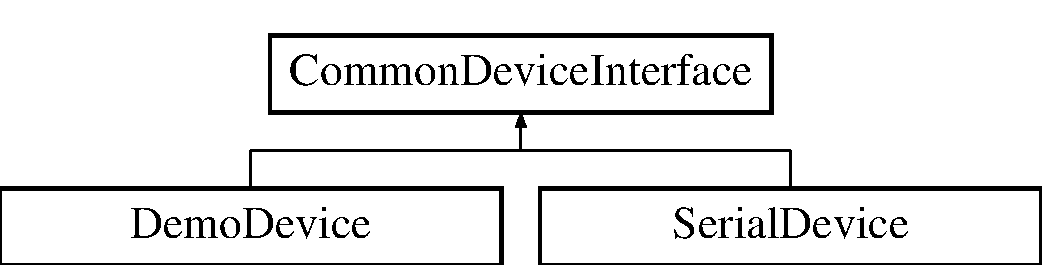
\includegraphics[height=2.000000cm]{class_common_device_interface}
\end{center}
\end{figure}
\subsection*{Public Member Functions}
\begin{DoxyCompactItemize}
\item 
\hypertarget{class_common_device_interface_ab968d5a571d435044a1304941f2ef349}{}\label{class_common_device_interface_ab968d5a571d435044a1304941f2ef349} 
virtual void {\bfseries sync} ()=0
\item 
\hypertarget{class_common_device_interface_ae58207ead16a77fa94babe01f0a3ba40}{}\label{class_common_device_interface_ae58207ead16a77fa94babe01f0a3ba40} 
virtual bool {\bfseries is\+Ready} ()=0
\item 
\hypertarget{class_common_device_interface_aa25434f588f2b8e4daa77f57f595d161}{}\label{class_common_device_interface_aa25434f588f2b8e4daa77f57f595d161} 
virtual bool {\bfseries start\+Device} ()=0
\item 
\hypertarget{class_common_device_interface_a53aaf8eee7297f3ee272cc4f366506bf}{}\label{class_common_device_interface_a53aaf8eee7297f3ee272cc4f366506bf} 
virtual void {\bfseries stop\+Device} ()=0
\item 
\hypertarget{class_common_device_interface_a542621a8b9e023531cae26447b2f8447}{}\label{class_common_device_interface_a542621a8b9e023531cae26447b2f8447} 
virtual void {\bfseries set\+Defaults} ()=0
\item 
\hypertarget{class_common_device_interface_ad670a54efd57ef65a659623f2a0b76e9}{}\label{class_common_device_interface_ad670a54efd57ef65a659623f2a0b76e9} 
virtual bool {\bfseries empty} ()=0
\item 
\hypertarget{class_common_device_interface_a110788eb0ee7ac9ecef7f47caad3a761}{}\label{class_common_device_interface_a110788eb0ee7ac9ecef7f47caad3a761} 
virtual void {\bfseries flush} ()=0
\item 
\hypertarget{class_common_device_interface_aae55f64252c8d094aa9d725b3c66e47f}{}\label{class_common_device_interface_aae55f64252c8d094aa9d725b3c66e47f} 
virtual void {\bfseries push\+Int} (int)=0
\item 
\hypertarget{class_common_device_interface_a02469d918befd346aee3253ddeb2bf03}{}\label{class_common_device_interface_a02469d918befd346aee3253ddeb2bf03} 
virtual void {\bfseries push\+Float} (float)=0
\item 
\hypertarget{class_common_device_interface_a2c6d30005d5cae436cd6d09b474967cc}{}\label{class_common_device_interface_a2c6d30005d5cae436cd6d09b474967cc} 
virtual void {\bfseries push\+Command} (flybyte)=0
\item 
\hypertarget{class_common_device_interface_ae944b4f2b1794cf2da1b3c3af4bf0bb5}{}\label{class_common_device_interface_ae944b4f2b1794cf2da1b3c3af4bf0bb5} 
virtual void {\bfseries push\+Command\+Immediate} (flybyte)=0
\item 
\hypertarget{class_common_device_interface_ac930cbe65cec618ae2069b05e3c30a9a}{}\label{class_common_device_interface_ac930cbe65cec618ae2069b05e3c30a9a} 
virtual flybyte {\bfseries pop\+Command} ()=0
\item 
\hypertarget{class_common_device_interface_a3d80b22eafc88af3109b08491bef6e8a}{}\label{class_common_device_interface_a3d80b22eafc88af3109b08491bef6e8a} 
virtual Q\+String {\bfseries name} ()=0
\end{DoxyCompactItemize}


The documentation for this class was generated from the following file\+:\begin{DoxyCompactItemize}
\item 
F\+E\+S\+S-\/\+G\+U\+I/commondeviceinterface.\+h\end{DoxyCompactItemize}

\hypertarget{class_common_interface_manager}{}\section{Common\+Interface\+Manager Class Reference}
\label{class_common_interface_manager}\index{Common\+Interface\+Manager@{Common\+Interface\+Manager}}


\hyperlink{class_common_interface_manager}{Common\+Interface\+Manager} Class Manages interfaces set in the interface selector menu.  




{\ttfamily \#include $<$commoninterfacemanager.\+h$>$}

\subsection*{Public Member Functions}
\begin{DoxyCompactItemize}
\item 
\hyperlink{class_common_interface_manager_a3f970287bd77d17ea41a6795b25ce7e3}{Common\+Interface\+Manager} ()
\begin{DoxyCompactList}\small\item\em \hyperlink{class_common_interface_manager_a3f970287bd77d17ea41a6795b25ce7e3}{Common\+Interface\+Manager\+::\+Common\+Interface\+Manager} Set the device to N\+U\+LL. \end{DoxyCompactList}\item 
\hyperlink{class_common_interface_manager_ad92cabe2e4f39fd762cf621df5125fa1}{$\sim$\+Common\+Interface\+Manager} ()
\begin{DoxyCompactList}\small\item\em \hyperlink{class_common_interface_manager_ad92cabe2e4f39fd762cf621df5125fa1}{Common\+Interface\+Manager\+::$\sim$\+Common\+Interface\+Manager} Deletes the current device. \end{DoxyCompactList}\item 
\hyperlink{class_common_device_interface}{Common\+Device\+Interface} $\ast$ \hyperlink{class_common_interface_manager_a24a72b0f78f9e6037e2da899e8170b2f}{get\+Current\+Interface} ()
\begin{DoxyCompactList}\small\item\em \hyperlink{class_common_interface_manager_a24a72b0f78f9e6037e2da899e8170b2f}{Common\+Interface\+Manager\+::get\+Current\+Interface} Get the current interface. \end{DoxyCompactList}\item 
void \hyperlink{class_common_interface_manager_add704853a060d8cca441da322b748c19}{set\+Current\+Interface} (\hyperlink{class_common_device_interface}{Common\+Device\+Interface} $\ast$)
\begin{DoxyCompactList}\small\item\em \hyperlink{class_common_interface_manager_add704853a060d8cca441da322b748c19}{Common\+Interface\+Manager\+::set\+Current\+Interface} Sets the curret device interface. \end{DoxyCompactList}\item 
bool \hyperlink{class_common_interface_manager_abd7a314803309cdb6789eaf36f90b7b7}{is\+A\+Device\+Set} ()
\begin{DoxyCompactList}\small\item\em \hyperlink{class_common_interface_manager_abd7a314803309cdb6789eaf36f90b7b7}{Common\+Interface\+Manager\+::is\+A\+Device\+Set} Determines if a device has been set in the menu. \end{DoxyCompactList}\item 
void \hyperlink{class_common_interface_manager_a16ab6917c45e1b40efe61d5379206ceb}{close\+Current\+Interface} ()
\begin{DoxyCompactList}\small\item\em \hyperlink{class_common_interface_manager_a16ab6917c45e1b40efe61d5379206ceb}{Common\+Interface\+Manager\+::close\+Current\+Interface} Closes the current interface. \end{DoxyCompactList}\end{DoxyCompactItemize}


\subsection{Detailed Description}
\hyperlink{class_common_interface_manager}{Common\+Interface\+Manager} Class Manages interfaces set in the interface selector menu. 

\subsection{Constructor \& Destructor Documentation}
\hypertarget{class_common_interface_manager_a3f970287bd77d17ea41a6795b25ce7e3}{}\label{class_common_interface_manager_a3f970287bd77d17ea41a6795b25ce7e3} 
\index{Common\+Interface\+Manager@{Common\+Interface\+Manager}!Common\+Interface\+Manager@{Common\+Interface\+Manager}}
\index{Common\+Interface\+Manager@{Common\+Interface\+Manager}!Common\+Interface\+Manager@{Common\+Interface\+Manager}}
\subsubsection{\texorpdfstring{Common\+Interface\+Manager()}{CommonInterfaceManager()}}
{\footnotesize\ttfamily Common\+Interface\+Manager\+::\+Common\+Interface\+Manager (\begin{DoxyParamCaption}{ }\end{DoxyParamCaption})}



\hyperlink{class_common_interface_manager_a3f970287bd77d17ea41a6795b25ce7e3}{Common\+Interface\+Manager\+::\+Common\+Interface\+Manager} Set the device to N\+U\+LL. 

\hypertarget{class_common_interface_manager_ad92cabe2e4f39fd762cf621df5125fa1}{}\label{class_common_interface_manager_ad92cabe2e4f39fd762cf621df5125fa1} 
\index{Common\+Interface\+Manager@{Common\+Interface\+Manager}!````~Common\+Interface\+Manager@{$\sim$\+Common\+Interface\+Manager}}
\index{````~Common\+Interface\+Manager@{$\sim$\+Common\+Interface\+Manager}!Common\+Interface\+Manager@{Common\+Interface\+Manager}}
\subsubsection{\texorpdfstring{$\sim$\+Common\+Interface\+Manager()}{~CommonInterfaceManager()}}
{\footnotesize\ttfamily Common\+Interface\+Manager\+::$\sim$\+Common\+Interface\+Manager (\begin{DoxyParamCaption}{ }\end{DoxyParamCaption})}



\hyperlink{class_common_interface_manager_ad92cabe2e4f39fd762cf621df5125fa1}{Common\+Interface\+Manager\+::$\sim$\+Common\+Interface\+Manager} Deletes the current device. 



\subsection{Member Function Documentation}
\hypertarget{class_common_interface_manager_a16ab6917c45e1b40efe61d5379206ceb}{}\label{class_common_interface_manager_a16ab6917c45e1b40efe61d5379206ceb} 
\index{Common\+Interface\+Manager@{Common\+Interface\+Manager}!close\+Current\+Interface@{close\+Current\+Interface}}
\index{close\+Current\+Interface@{close\+Current\+Interface}!Common\+Interface\+Manager@{Common\+Interface\+Manager}}
\subsubsection{\texorpdfstring{close\+Current\+Interface()}{closeCurrentInterface()}}
{\footnotesize\ttfamily void Common\+Interface\+Manager\+::close\+Current\+Interface (\begin{DoxyParamCaption}{ }\end{DoxyParamCaption})}



\hyperlink{class_common_interface_manager_a16ab6917c45e1b40efe61d5379206ceb}{Common\+Interface\+Manager\+::close\+Current\+Interface} Closes the current interface. 

\hypertarget{class_common_interface_manager_a24a72b0f78f9e6037e2da899e8170b2f}{}\label{class_common_interface_manager_a24a72b0f78f9e6037e2da899e8170b2f} 
\index{Common\+Interface\+Manager@{Common\+Interface\+Manager}!get\+Current\+Interface@{get\+Current\+Interface}}
\index{get\+Current\+Interface@{get\+Current\+Interface}!Common\+Interface\+Manager@{Common\+Interface\+Manager}}
\subsubsection{\texorpdfstring{get\+Current\+Interface()}{getCurrentInterface()}}
{\footnotesize\ttfamily \hyperlink{class_common_device_interface}{Common\+Device\+Interface} $\ast$ Common\+Interface\+Manager\+::get\+Current\+Interface (\begin{DoxyParamCaption}{ }\end{DoxyParamCaption})}



\hyperlink{class_common_interface_manager_a24a72b0f78f9e6037e2da899e8170b2f}{Common\+Interface\+Manager\+::get\+Current\+Interface} Get the current interface. 

\begin{DoxyReturn}{Returns}
Common\+Device\+Interface$\ast$ (\hyperlink{class_common_device_interface}{Common\+Device\+Interface} Instance Pointer,N\+U\+LL) 
\end{DoxyReturn}
\hypertarget{class_common_interface_manager_abd7a314803309cdb6789eaf36f90b7b7}{}\label{class_common_interface_manager_abd7a314803309cdb6789eaf36f90b7b7} 
\index{Common\+Interface\+Manager@{Common\+Interface\+Manager}!is\+A\+Device\+Set@{is\+A\+Device\+Set}}
\index{is\+A\+Device\+Set@{is\+A\+Device\+Set}!Common\+Interface\+Manager@{Common\+Interface\+Manager}}
\subsubsection{\texorpdfstring{is\+A\+Device\+Set()}{isADeviceSet()}}
{\footnotesize\ttfamily bool Common\+Interface\+Manager\+::is\+A\+Device\+Set (\begin{DoxyParamCaption}{ }\end{DoxyParamCaption})}



\hyperlink{class_common_interface_manager_abd7a314803309cdb6789eaf36f90b7b7}{Common\+Interface\+Manager\+::is\+A\+Device\+Set} Determines if a device has been set in the menu. 

\begin{DoxyReturn}{Returns}
bool (true=Yes, false=No) 
\end{DoxyReturn}
\hypertarget{class_common_interface_manager_add704853a060d8cca441da322b748c19}{}\label{class_common_interface_manager_add704853a060d8cca441da322b748c19} 
\index{Common\+Interface\+Manager@{Common\+Interface\+Manager}!set\+Current\+Interface@{set\+Current\+Interface}}
\index{set\+Current\+Interface@{set\+Current\+Interface}!Common\+Interface\+Manager@{Common\+Interface\+Manager}}
\subsubsection{\texorpdfstring{set\+Current\+Interface()}{setCurrentInterface()}}
{\footnotesize\ttfamily void Common\+Interface\+Manager\+::set\+Current\+Interface (\begin{DoxyParamCaption}\item[{\hyperlink{class_common_device_interface}{Common\+Device\+Interface} $\ast$}]{new\+Interface }\end{DoxyParamCaption})}



\hyperlink{class_common_interface_manager_add704853a060d8cca441da322b748c19}{Common\+Interface\+Manager\+::set\+Current\+Interface} Sets the curret device interface. 


\begin{DoxyParams}{Parameters}
{\em Common\+Device\+Interface$\ast$} & \\
\hline
\end{DoxyParams}


The documentation for this class was generated from the following files\+:\begin{DoxyCompactItemize}
\item 
F\+E\+S\+S-\/\+G\+U\+I/\hyperlink{commoninterfacemanager_8h}{commoninterfacemanager.\+h}\item 
F\+E\+S\+S-\/\+G\+U\+I/\hyperlink{commoninterfacemanager_8cpp}{commoninterfacemanager.\+cpp}\end{DoxyCompactItemize}

\hypertarget{class_common_interface_selector}{}\section{Common\+Interface\+Selector Class Reference}
\label{class_common_interface_selector}\index{Common\+Interface\+Selector@{Common\+Interface\+Selector}}
Inheritance diagram for Common\+Interface\+Selector\+:\begin{figure}[H]
\begin{center}
\leavevmode
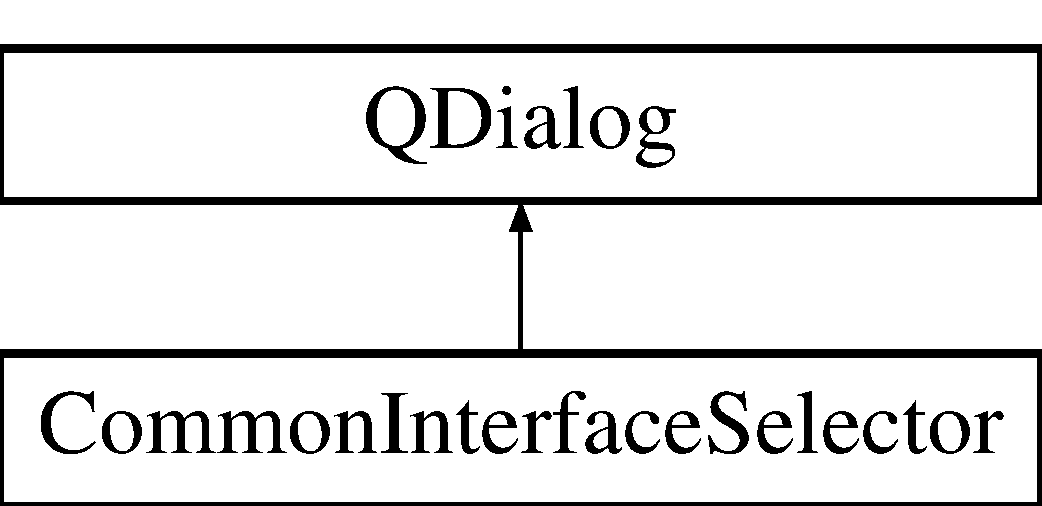
\includegraphics[height=2.000000cm]{class_common_interface_selector}
\end{center}
\end{figure}
\subsection*{Public Member Functions}
\begin{DoxyCompactItemize}
\item 
\hypertarget{class_common_interface_selector_a46da3e73aa0868810dbd80a42281a6c8}{}\label{class_common_interface_selector_a46da3e73aa0868810dbd80a42281a6c8} 
{\bfseries Common\+Interface\+Selector} (\hyperlink{class_common_interface_manager}{Common\+Interface\+Manager} $\ast$, Q\+Widget $\ast$parent=0)
\end{DoxyCompactItemize}


The documentation for this class was generated from the following files\+:\begin{DoxyCompactItemize}
\item 
C\+:/\+Users/\+Jesse Jutson/\+Documents/\+Git\+Hub/\+F\+E\+S\+S\+G\+U\+I/\+F\+E\+S\+S-\/\+G\+U\+I/commoninterfaceselector.\+h\item 
C\+:/\+Users/\+Jesse Jutson/\+Documents/\+Git\+Hub/\+F\+E\+S\+S\+G\+U\+I/\+F\+E\+S\+S-\/\+G\+U\+I/commoninterfaceselector.\+cpp\end{DoxyCompactItemize}

\hypertarget{class_demo_device}{}\section{Demo\+Device Class Reference}
\label{class_demo_device}\index{Demo\+Device@{Demo\+Device}}
Inheritance diagram for Demo\+Device\+:\begin{figure}[H]
\begin{center}
\leavevmode
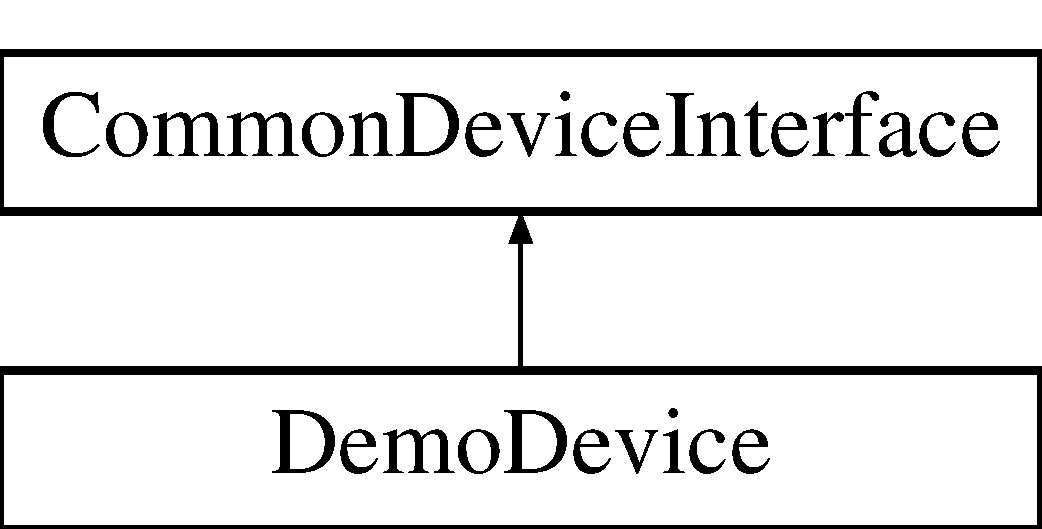
\includegraphics[height=2.000000cm]{class_demo_device}
\end{center}
\end{figure}
\subsection*{Public Member Functions}
\begin{DoxyCompactItemize}
\item 
\hypertarget{class_demo_device_a9fc771c4152f0d9de78a69187cbd7a58}{}\label{class_demo_device_a9fc771c4152f0d9de78a69187cbd7a58} 
\hyperlink{class_demo_device_a9fc771c4152f0d9de78a69187cbd7a58}{Demo\+Device} ()
\begin{DoxyCompactList}\small\item\em \hyperlink{class_demo_device_a9fc771c4152f0d9de78a69187cbd7a58}{Demo\+Device\+::\+Demo\+Device} Configures a new \hyperlink{class_demo_device}{Demo\+Device} with its default values. \end{DoxyCompactList}\item 
\hypertarget{class_demo_device_aff994361f45ae993feb854f72a2a32a6}{}\label{class_demo_device_aff994361f45ae993feb854f72a2a32a6} 
\hyperlink{class_demo_device_aff994361f45ae993feb854f72a2a32a6}{$\sim$\+Demo\+Device} ()
\begin{DoxyCompactList}\small\item\em \hyperlink{class_demo_device_aff994361f45ae993feb854f72a2a32a6}{Demo\+Device\+::$\sim$\+Demo\+Device} Provided if needed in the future, currently no functionality. \end{DoxyCompactList}\item 
\hypertarget{class_demo_device_a85671c408f6f08d82a09344ef5f34966}{}\label{class_demo_device_a85671c408f6f08d82a09344ef5f34966} 
void \hyperlink{class_demo_device_a85671c408f6f08d82a09344ef5f34966}{sync\+RX} ()
\begin{DoxyCompactList}\small\item\em \hyperlink{class_demo_device_a85671c408f6f08d82a09344ef5f34966}{Demo\+Device\+::sync\+RX} Is the demo interface\textquotesingle{}s implementation of sync\+RX. Generates values for testing and pushes them into the interface\textquotesingle{}s RX Transmit Buffer. \end{DoxyCompactList}\item 
\hypertarget{class_demo_device_a4b33b0148627fcbd22a0704e80f05d7d}{}\label{class_demo_device_a4b33b0148627fcbd22a0704e80f05d7d} 
void \hyperlink{class_demo_device_a4b33b0148627fcbd22a0704e80f05d7d}{sync\+TX} ()
\begin{DoxyCompactList}\small\item\em \hyperlink{class_demo_device_a85671c408f6f08d82a09344ef5f34966}{Demo\+Device\+::sync\+RX} Is the demo interface\textquotesingle{}s implementation of sync\+RX. Reacts to the interfaces commands (Only Emergency Stop currently) \end{DoxyCompactList}\item 
bool \hyperlink{class_demo_device_aaadb9ced56699af55526b9fc7cf8420c}{is\+Ready} ()
\begin{DoxyCompactList}\small\item\em \hyperlink{class_demo_device_aaadb9ced56699af55526b9fc7cf8420c}{Demo\+Device\+::is\+Ready} Is the demo interface\textquotesingle{}s implementation of is\+Ready. Get the status of the demo interface. \end{DoxyCompactList}\item 
bool \hyperlink{class_demo_device_af350ecf6ff289983cff9053197f1b1f2}{start\+Device} ()
\begin{DoxyCompactList}\small\item\em \hyperlink{class_demo_device_af350ecf6ff289983cff9053197f1b1f2}{Demo\+Device\+::start\+Device} Is the demo interface\textquotesingle{}s implementation of start\+Device. Starts the demo interface and updates status. \end{DoxyCompactList}\item 
\hypertarget{class_demo_device_ab95434f7121f00789108f29a8457ec98}{}\label{class_demo_device_ab95434f7121f00789108f29a8457ec98} 
void \hyperlink{class_demo_device_ab95434f7121f00789108f29a8457ec98}{stop\+Device} ()
\begin{DoxyCompactList}\small\item\em \hyperlink{class_demo_device_ab95434f7121f00789108f29a8457ec98}{Demo\+Device\+::stop\+Device} Is the demo interface\textquotesingle{}s implementation of stop\+Device. Stops the demo interface and updates status. \end{DoxyCompactList}\item 
\hypertarget{class_demo_device_a79a9c22e60aca99c7667990bedc461c8}{}\label{class_demo_device_a79a9c22e60aca99c7667990bedc461c8} 
void \hyperlink{class_demo_device_a79a9c22e60aca99c7667990bedc461c8}{set\+Defaults} ()
\begin{DoxyCompactList}\small\item\em \hyperlink{class_demo_device_ab95434f7121f00789108f29a8457ec98}{Demo\+Device\+::stop\+Device} Is the demo interface\textquotesingle{}s implementation of set\+Defaults. Sets the serial devices to the default values. \end{DoxyCompactList}\item 
bool \hyperlink{class_demo_device_a52de363ec31fdbb540cf7cae6f584d22}{empty} ()
\begin{DoxyCompactList}\small\item\em \hyperlink{class_demo_device_a52de363ec31fdbb540cf7cae6f584d22}{Demo\+Device\+::empty} Is the demo interface\textquotesingle{}s implementation of empty. \end{DoxyCompactList}\item 
\hypertarget{class_demo_device_abd7460c71a01d986b1f77908ccb779a2}{}\label{class_demo_device_abd7460c71a01d986b1f77908ccb779a2} 
void \hyperlink{class_demo_device_abd7460c71a01d986b1f77908ccb779a2}{flush\+RX} ()
\begin{DoxyCompactList}\small\item\em \hyperlink{class_demo_device_abd7460c71a01d986b1f77908ccb779a2}{Demo\+Device\+::flush\+RX} Is the demo interface\textquotesingle{}s implementation of flush\+RX. Empties the RX Transmit Buffer. \end{DoxyCompactList}\item 
\hypertarget{class_demo_device_a32e89c17f613abfa7f2a4d9f970bbffe}{}\label{class_demo_device_a32e89c17f613abfa7f2a4d9f970bbffe} 
void \hyperlink{class_demo_device_a32e89c17f613abfa7f2a4d9f970bbffe}{flush\+TX} ()
\begin{DoxyCompactList}\small\item\em \hyperlink{class_demo_device_a32e89c17f613abfa7f2a4d9f970bbffe}{Demo\+Device\+::flush\+TX} Is the demo interface\textquotesingle{}s implementation of flush\+TX. Empties the TX Transmit Buffer. \end{DoxyCompactList}\item 
void \hyperlink{class_demo_device_a064f0bc683663200243bd68ff3713c68}{push\+Byte} (Fly\+Byte)
\begin{DoxyCompactList}\small\item\em \hyperlink{class_demo_device_a788dd7e426fab9c8d19ea9fd106260d4}{Demo\+Device\+::pop\+Byte} Is the demo interface\textquotesingle{}s implementation of push\+Byte. \end{DoxyCompactList}\item 
void \hyperlink{class_demo_device_ac39f46589b28926cd40635ad42342a54}{push\+Packet} (\hyperlink{class_fly_packet}{Fly\+Packet})
\begin{DoxyCompactList}\small\item\em \hyperlink{class_demo_device_a788dd7e426fab9c8d19ea9fd106260d4}{Demo\+Device\+::pop\+Byte} Is the demo interface\textquotesingle{}s implementation of push\+Packet. \end{DoxyCompactList}\item 
Fly\+Byte \hyperlink{class_demo_device_a788dd7e426fab9c8d19ea9fd106260d4}{pop\+Byte} ()
\begin{DoxyCompactList}\small\item\em \hyperlink{class_demo_device_a788dd7e426fab9c8d19ea9fd106260d4}{Demo\+Device\+::pop\+Byte} Is the demo interface\textquotesingle{}s implementation of pop\+Byte. \end{DoxyCompactList}\item 
\hyperlink{class_fly_packet}{Fly\+Packet} \hyperlink{class_demo_device_a6e755f50f52301b9166e278fe6851e88}{pop\+Packet} ()
\begin{DoxyCompactList}\small\item\em \hyperlink{class_demo_device_a788dd7e426fab9c8d19ea9fd106260d4}{Demo\+Device\+::pop\+Byte} Is the demo interface\textquotesingle{}s implementation of pop\+Packet. \end{DoxyCompactList}\item 
Q\+String \hyperlink{class_demo_device_acde538bd5a71a8d4df6293876169545c}{name} ()
\begin{DoxyCompactList}\small\item\em \hyperlink{class_demo_device_acde538bd5a71a8d4df6293876169545c}{Demo\+Device\+::name} Is the demo interface\textquotesingle{}s implementation of name. \end{DoxyCompactList}\end{DoxyCompactItemize}


\subsection{Member Function Documentation}
\hypertarget{class_demo_device_a52de363ec31fdbb540cf7cae6f584d22}{}\label{class_demo_device_a52de363ec31fdbb540cf7cae6f584d22} 
\index{Demo\+Device@{Demo\+Device}!empty@{empty}}
\index{empty@{empty}!Demo\+Device@{Demo\+Device}}
\subsubsection{\texorpdfstring{empty()}{empty()}}
{\footnotesize\ttfamily bool Demo\+Device\+::empty (\begin{DoxyParamCaption}{ }\end{DoxyParamCaption})\hspace{0.3cm}{\ttfamily [virtual]}}



\hyperlink{class_demo_device_a52de363ec31fdbb540cf7cae6f584d22}{Demo\+Device\+::empty} Is the demo interface\textquotesingle{}s implementation of empty. 

\begin{DoxyReturn}{Returns}
bool (true=Empty, false=Not Empty) 
\end{DoxyReturn}


Implements \hyperlink{class_common_device_interface}{Common\+Device\+Interface}.

\hypertarget{class_demo_device_aaadb9ced56699af55526b9fc7cf8420c}{}\label{class_demo_device_aaadb9ced56699af55526b9fc7cf8420c} 
\index{Demo\+Device@{Demo\+Device}!is\+Ready@{is\+Ready}}
\index{is\+Ready@{is\+Ready}!Demo\+Device@{Demo\+Device}}
\subsubsection{\texorpdfstring{is\+Ready()}{isReady()}}
{\footnotesize\ttfamily bool Demo\+Device\+::is\+Ready (\begin{DoxyParamCaption}{ }\end{DoxyParamCaption})\hspace{0.3cm}{\ttfamily [virtual]}}



\hyperlink{class_demo_device_aaadb9ced56699af55526b9fc7cf8420c}{Demo\+Device\+::is\+Ready} Is the demo interface\textquotesingle{}s implementation of is\+Ready. Get the status of the demo interface. 

\begin{DoxyReturn}{Returns}
bool (true=Ready, false=Not Ready) 
\end{DoxyReturn}


Implements \hyperlink{class_common_device_interface}{Common\+Device\+Interface}.

\hypertarget{class_demo_device_acde538bd5a71a8d4df6293876169545c}{}\label{class_demo_device_acde538bd5a71a8d4df6293876169545c} 
\index{Demo\+Device@{Demo\+Device}!name@{name}}
\index{name@{name}!Demo\+Device@{Demo\+Device}}
\subsubsection{\texorpdfstring{name()}{name()}}
{\footnotesize\ttfamily Q\+String Demo\+Device\+::name (\begin{DoxyParamCaption}{ }\end{DoxyParamCaption})\hspace{0.3cm}{\ttfamily [virtual]}}



\hyperlink{class_demo_device_acde538bd5a71a8d4df6293876169545c}{Demo\+Device\+::name} Is the demo interface\textquotesingle{}s implementation of name. 

\begin{DoxyReturn}{Returns}
Qstring (\char`\"{}\+Demo Device\char`\"{}) 
\end{DoxyReturn}


Implements \hyperlink{class_common_device_interface}{Common\+Device\+Interface}.

\hypertarget{class_demo_device_a788dd7e426fab9c8d19ea9fd106260d4}{}\label{class_demo_device_a788dd7e426fab9c8d19ea9fd106260d4} 
\index{Demo\+Device@{Demo\+Device}!pop\+Byte@{pop\+Byte}}
\index{pop\+Byte@{pop\+Byte}!Demo\+Device@{Demo\+Device}}
\subsubsection{\texorpdfstring{pop\+Byte()}{popByte()}}
{\footnotesize\ttfamily Fly\+Byte Demo\+Device\+::pop\+Byte (\begin{DoxyParamCaption}{ }\end{DoxyParamCaption})\hspace{0.3cm}{\ttfamily [virtual]}}



\hyperlink{class_demo_device_a788dd7e426fab9c8d19ea9fd106260d4}{Demo\+Device\+::pop\+Byte} Is the demo interface\textquotesingle{}s implementation of pop\+Byte. 

\begin{DoxyReturn}{Returns}
Fly\+Byte (From the RX Transmit Buffer). 
\end{DoxyReturn}


Implements \hyperlink{class_common_device_interface}{Common\+Device\+Interface}.

\hypertarget{class_demo_device_a6e755f50f52301b9166e278fe6851e88}{}\label{class_demo_device_a6e755f50f52301b9166e278fe6851e88} 
\index{Demo\+Device@{Demo\+Device}!pop\+Packet@{pop\+Packet}}
\index{pop\+Packet@{pop\+Packet}!Demo\+Device@{Demo\+Device}}
\subsubsection{\texorpdfstring{pop\+Packet()}{popPacket()}}
{\footnotesize\ttfamily \hyperlink{class_fly_packet}{Fly\+Packet} Demo\+Device\+::pop\+Packet (\begin{DoxyParamCaption}{ }\end{DoxyParamCaption})\hspace{0.3cm}{\ttfamily [virtual]}}



\hyperlink{class_demo_device_a788dd7e426fab9c8d19ea9fd106260d4}{Demo\+Device\+::pop\+Byte} Is the demo interface\textquotesingle{}s implementation of pop\+Packet. 

\begin{DoxyReturn}{Returns}
\hyperlink{class_fly_packet}{Fly\+Packet} (From the RX Transmit Buffer). 
\end{DoxyReturn}


Implements \hyperlink{class_common_device_interface}{Common\+Device\+Interface}.

\hypertarget{class_demo_device_a064f0bc683663200243bd68ff3713c68}{}\label{class_demo_device_a064f0bc683663200243bd68ff3713c68} 
\index{Demo\+Device@{Demo\+Device}!push\+Byte@{push\+Byte}}
\index{push\+Byte@{push\+Byte}!Demo\+Device@{Demo\+Device}}
\subsubsection{\texorpdfstring{push\+Byte()}{pushByte()}}
{\footnotesize\ttfamily void Demo\+Device\+::push\+Byte (\begin{DoxyParamCaption}\item[{Fly\+Byte}]{data\+Byte }\end{DoxyParamCaption})\hspace{0.3cm}{\ttfamily [virtual]}}



\hyperlink{class_demo_device_a788dd7e426fab9c8d19ea9fd106260d4}{Demo\+Device\+::pop\+Byte} Is the demo interface\textquotesingle{}s implementation of push\+Byte. 


\begin{DoxyParams}{Parameters}
{\em Fly\+Byte} & (Adds it to the TX Transmit Buffer). \\
\hline
\end{DoxyParams}


Implements \hyperlink{class_common_device_interface}{Common\+Device\+Interface}.

\hypertarget{class_demo_device_ac39f46589b28926cd40635ad42342a54}{}\label{class_demo_device_ac39f46589b28926cd40635ad42342a54} 
\index{Demo\+Device@{Demo\+Device}!push\+Packet@{push\+Packet}}
\index{push\+Packet@{push\+Packet}!Demo\+Device@{Demo\+Device}}
\subsubsection{\texorpdfstring{push\+Packet()}{pushPacket()}}
{\footnotesize\ttfamily void Demo\+Device\+::push\+Packet (\begin{DoxyParamCaption}\item[{\hyperlink{class_fly_packet}{Fly\+Packet}}]{data\+Packet }\end{DoxyParamCaption})\hspace{0.3cm}{\ttfamily [virtual]}}



\hyperlink{class_demo_device_a788dd7e426fab9c8d19ea9fd106260d4}{Demo\+Device\+::pop\+Byte} Is the demo interface\textquotesingle{}s implementation of push\+Packet. 


\begin{DoxyParams}{Parameters}
{\em \hyperlink{class_fly_packet}{Fly\+Packet}} & (Adds to the TX Transmit Buffer). \\
\hline
\end{DoxyParams}


Implements \hyperlink{class_common_device_interface}{Common\+Device\+Interface}.

\hypertarget{class_demo_device_af350ecf6ff289983cff9053197f1b1f2}{}\label{class_demo_device_af350ecf6ff289983cff9053197f1b1f2} 
\index{Demo\+Device@{Demo\+Device}!start\+Device@{start\+Device}}
\index{start\+Device@{start\+Device}!Demo\+Device@{Demo\+Device}}
\subsubsection{\texorpdfstring{start\+Device()}{startDevice()}}
{\footnotesize\ttfamily bool Demo\+Device\+::start\+Device (\begin{DoxyParamCaption}{ }\end{DoxyParamCaption})\hspace{0.3cm}{\ttfamily [virtual]}}



\hyperlink{class_demo_device_af350ecf6ff289983cff9053197f1b1f2}{Demo\+Device\+::start\+Device} Is the demo interface\textquotesingle{}s implementation of start\+Device. Starts the demo interface and updates status. 

\begin{DoxyReturn}{Returns}
bool (true=Started, false=Not Ready) 
\end{DoxyReturn}


Implements \hyperlink{class_common_device_interface}{Common\+Device\+Interface}.



The documentation for this class was generated from the following files\+:\begin{DoxyCompactItemize}
\item 
F\+E\+S\+S-\/\+G\+U\+I/demodevice.\+h\item 
F\+E\+S\+S-\/\+G\+U\+I/demodevice.\+cpp\end{DoxyCompactItemize}

\hypertarget{structflypacket}{}\section{flypacket Struct Reference}
\label{structflypacket}\index{flypacket@{flypacket}}
\subsection*{Public Attributes}
\begin{DoxyCompactItemize}
\item 
\hypertarget{structflypacket_a1c430b5e9b74fe1822f09c23ac3ffca9}{}\label{structflypacket_a1c430b5e9b74fe1822f09c23ac3ffca9} 
flybyte {\bfseries packet\+Type}
\item 
\hypertarget{structflypacket_a9b4d29c0e457223adfedc0ce82117f49}{}\label{structflypacket_a9b4d29c0e457223adfedc0ce82117f49} 
flybyte {\bfseries data\+Type}
\item 
\hypertarget{structflypacket_a6e6310660096115b4360c9d392281463}{}\label{structflypacket_a6e6310660096115b4360c9d392281463} 
float {\bfseries data\+Value}
\end{DoxyCompactItemize}


The documentation for this struct was generated from the following file\+:\begin{DoxyCompactItemize}
\item 
C\+:/\+Users/\+Jesse Jutson/\+Documents/\+Git\+Hub/\+F\+E\+S\+S\+G\+U\+I/\+F\+E\+S\+S-\/\+G\+U\+I/datatypes.\+h\end{DoxyCompactItemize}

\hypertarget{class_flywheel_operation}{}\section{Flywheel\+Operation Class Reference}
\label{class_flywheel_operation}\index{Flywheel\+Operation@{Flywheel\+Operation}}
\subsection*{Public Member Functions}
\begin{DoxyCompactItemize}
\item 
\hypertarget{class_flywheel_operation_aca3144bf0bb443aaa8a2779624d2a5b2}{}\label{class_flywheel_operation_aca3144bf0bb443aaa8a2779624d2a5b2} 
{\bfseries Flywheel\+Operation} (\hyperlink{class_common_device_interface}{Common\+Device\+Interface} $\ast$)
\item 
\hypertarget{class_flywheel_operation_a61df04a204188bd187ce68f9d610e78a}{}\label{class_flywheel_operation_a61df04a204188bd187ce68f9d610e78a} 
void {\bfseries sync} ()
\item 
\hypertarget{class_flywheel_operation_a23b72640fdedd6d89575ea9a4ef3c69a}{}\label{class_flywheel_operation_a23b72640fdedd6d89575ea9a4ef3c69a} 
void {\bfseries set\+Defaults} ()
\item 
\hypertarget{class_flywheel_operation_a30e26868333a6a7d73ae34156ba432a8}{}\label{class_flywheel_operation_a30e26868333a6a7d73ae34156ba432a8} 
void {\bfseries set\+Velocity} (float)
\item 
\hypertarget{class_flywheel_operation_a307929c750339cb2b46baaafa526d29f}{}\label{class_flywheel_operation_a307929c750339cb2b46baaafa526d29f} 
void {\bfseries set\+Acceleration} (float)
\item 
\hypertarget{class_flywheel_operation_a4f14dfe672793f37e21f90ecab499378}{}\label{class_flywheel_operation_a4f14dfe672793f37e21f90ecab499378} 
void {\bfseries set\+Jerk} (float)
\item 
\hypertarget{class_flywheel_operation_a9bcbe2d59c2a14c08b9b34d2e0c63023}{}\label{class_flywheel_operation_a9bcbe2d59c2a14c08b9b34d2e0c63023} 
void {\bfseries set\+Motion} (float, float, float)
\item 
\hypertarget{class_flywheel_operation_a06119af2250971d23869d94fd451ceba}{}\label{class_flywheel_operation_a06119af2250971d23869d94fd451ceba} 
float {\bfseries get\+Velocity} ()
\item 
\hypertarget{class_flywheel_operation_a23310ab41f29ee3d510c2d412fde801b}{}\label{class_flywheel_operation_a23310ab41f29ee3d510c2d412fde801b} 
float {\bfseries get\+Acceleration} ()
\item 
\hypertarget{class_flywheel_operation_ad443ef22229c1584da213f50234720bf}{}\label{class_flywheel_operation_ad443ef22229c1584da213f50234720bf} 
float {\bfseries get\+Jerk} ()
\item 
\hypertarget{class_flywheel_operation_a6a393e52299f7a48950f019d0f3db7de}{}\label{class_flywheel_operation_a6a393e52299f7a48950f019d0f3db7de} 
void {\bfseries emergency\+Stop} ()
\item 
\hypertarget{class_flywheel_operation_ab655d2757d24dbb605a8eb0c16bc0fe8}{}\label{class_flywheel_operation_ab655d2757d24dbb605a8eb0c16bc0fe8} 
void {\bfseries set\+Interface} (\hyperlink{class_common_device_interface}{Common\+Device\+Interface} $\ast$)
\item 
\hypertarget{class_flywheel_operation_a16ebc2fe8c3297350eaf9be2114a75c8}{}\label{class_flywheel_operation_a16ebc2fe8c3297350eaf9be2114a75c8} 
Q\+PointF {\bfseries get\+Upper\+Displacement} ()
\item 
\hypertarget{class_flywheel_operation_a2b9d24d0fbbf1d9cb79bb0aa54f6f6ae}{}\label{class_flywheel_operation_a2b9d24d0fbbf1d9cb79bb0aa54f6f6ae} 
Q\+PointF {\bfseries get\+Lower\+Displacement} ()
\item 
\hypertarget{class_flywheel_operation_a0e1ba213763760cf0128dfdc8436cfdf}{}\label{class_flywheel_operation_a0e1ba213763760cf0128dfdc8436cfdf} 
Q\+PointF {\bfseries get\+Rotational\+Position} ()
\end{DoxyCompactItemize}


The documentation for this class was generated from the following files\+:\begin{DoxyCompactItemize}
\item 
F\+E\+S\+S-\/\+G\+U\+I/flywheeloperation.\+h\item 
F\+E\+S\+S-\/\+G\+U\+I/flywheeloperation.\+cpp\end{DoxyCompactItemize}

\hypertarget{class_graph}{}\section{Graph Class Reference}
\label{class_graph}\index{Graph@{Graph}}


The \hyperlink{class_graph}{Graph} class, base class for all graphs. Each graph contains a main plot (the large graph that is seen when a graph is selected) and a auxiliary plot (the smaller graph that is always visible on the right side).  




{\ttfamily \#include $<$graph.\+h$>$}

Inheritance diagram for Graph\+:\begin{figure}[H]
\begin{center}
\leavevmode
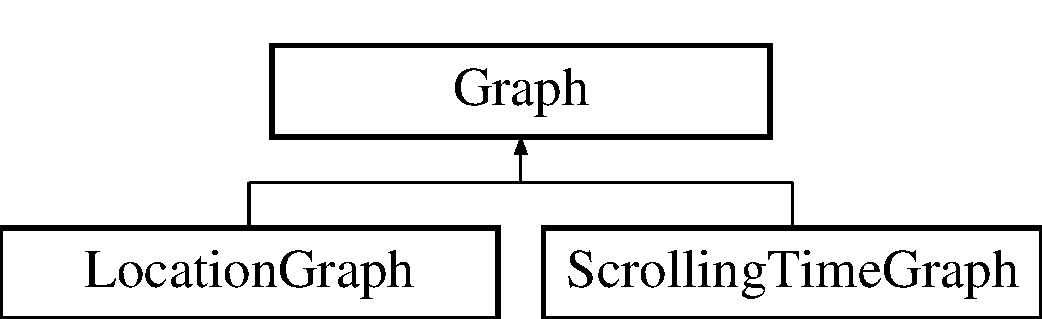
\includegraphics[height=2.000000cm]{class_graph}
\end{center}
\end{figure}
\subsection*{Public Member Functions}
\begin{DoxyCompactItemize}
\item 
\hypertarget{class_graph_ae4c72b8ac4d693c49800a4c7e273654f}{}\label{class_graph_ae4c72b8ac4d693c49800a4c7e273654f} 
\hyperlink{class_graph_ae4c72b8ac4d693c49800a4c7e273654f}{Graph} ()
\begin{DoxyCompactList}\small\item\em \hyperlink{class_graph_ae4c72b8ac4d693c49800a4c7e273654f}{Graph\+::\+Graph} Empty constructor for the base class. This should not be used. \end{DoxyCompactList}\item 
\hypertarget{class_graph_a5102e5e984c2ddebb79b9771b9d37f9f}{}\label{class_graph_a5102e5e984c2ddebb79b9771b9d37f9f} 
virtual Q\+String {\bfseries max\+Display} ()
\item 
\hypertarget{class_graph_a85028910472bc7815ad024ca025bb142}{}\label{class_graph_a85028910472bc7815ad024ca025bb142} 
virtual Q\+String {\bfseries current\+Display} ()
\end{DoxyCompactItemize}
\subsection*{Public Attributes}
\begin{DoxyCompactItemize}
\item 
\hypertarget{class_graph_ab42ef887ac4d6bad01cc0c2c3609ab6b}{}\label{class_graph_ab42ef887ac4d6bad01cc0c2c3609ab6b} 
Q\+Color {\bfseries primary\+Color}
\item 
\hypertarget{class_graph_a7bda51c2c124dfe46d5ee515a2508511}{}\label{class_graph_a7bda51c2c124dfe46d5ee515a2508511} 
Q\+Color {\bfseries secondary\+Color}
\end{DoxyCompactItemize}
\subsection*{Protected Attributes}
\begin{DoxyCompactItemize}
\item 
\hypertarget{class_graph_a02239013b745a7c1411a7f8623cc2073}{}\label{class_graph_a02239013b745a7c1411a7f8623cc2073} 
\hyperlink{class_q_custom_plot}{Q\+Custom\+Plot} $\ast$ {\bfseries main\+Plot}
\item 
\hypertarget{class_graph_ac7d10642e5439fd87d7d4bc5a33e643d}{}\label{class_graph_ac7d10642e5439fd87d7d4bc5a33e643d} 
\hyperlink{class_q_custom_plot}{Q\+Custom\+Plot} $\ast$ {\bfseries aux\+Plot}
\item 
\hypertarget{class_graph_a28488c31277fec31c8d54a44860efede}{}\label{class_graph_a28488c31277fec31c8d54a44860efede} 
Q\+String {\bfseries display\+Unit}
\end{DoxyCompactItemize}


\subsection{Detailed Description}
The \hyperlink{class_graph}{Graph} class, base class for all graphs. Each graph contains a main plot (the large graph that is seen when a graph is selected) and a auxiliary plot (the smaller graph that is always visible on the right side). 

The documentation for this class was generated from the following files\+:\begin{DoxyCompactItemize}
\item 
C\+:/\+Users/\+Jesse Jutson/\+Documents/\+Git\+Hub/\+F\+E\+S\+S\+G\+U\+I/\+F\+E\+S\+S-\/\+G\+U\+I/graph.\+h\item 
C\+:/\+Users/\+Jesse Jutson/\+Documents/\+Git\+Hub/\+F\+E\+S\+S\+G\+U\+I/\+F\+E\+S\+S-\/\+G\+U\+I/graph.\+cpp\end{DoxyCompactItemize}

\hypertarget{class_location_graph}{}\section{Location\+Graph Class Reference}
\label{class_location_graph}\index{Location\+Graph@{Location\+Graph}}


The \hyperlink{class_location_graph}{Location\+Graph} class, which inherits from the \hyperlink{class_graph}{Graph} class. This represents a graph where the x and y axes represent location. This is a real-\/time graph, with no view of what happened in the past.  




{\ttfamily \#include $<$graph.\+h$>$}

Inheritance diagram for Location\+Graph\+:\begin{figure}[H]
\begin{center}
\leavevmode
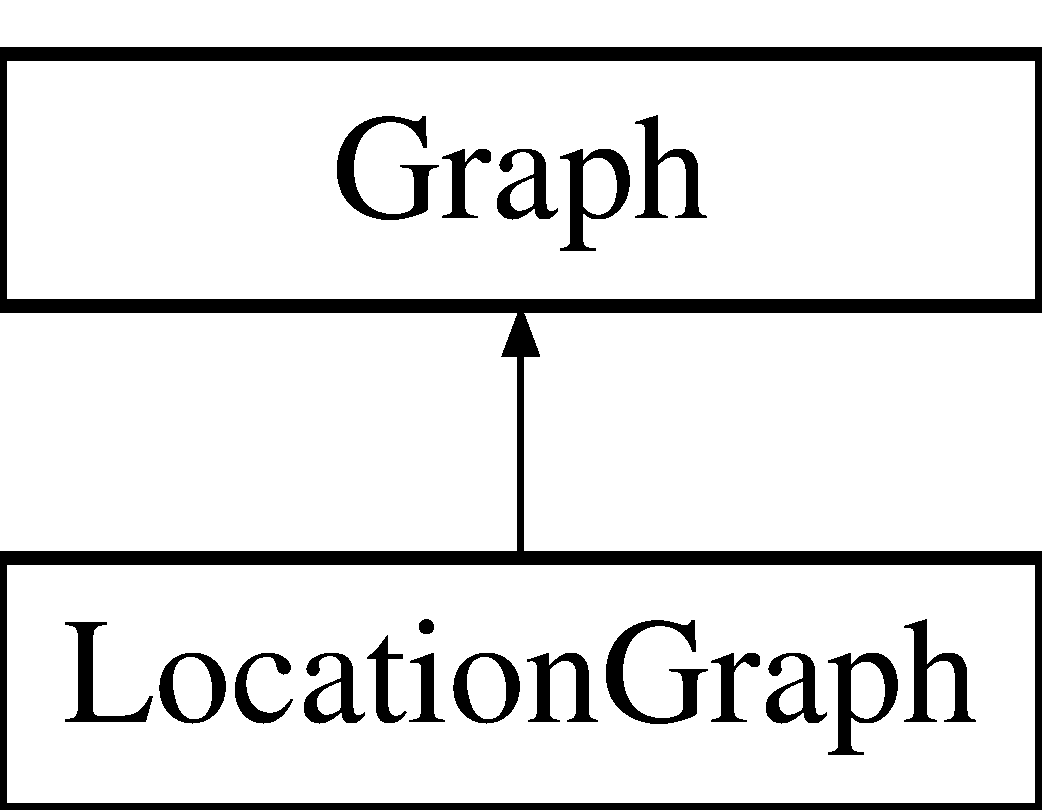
\includegraphics[height=2.000000cm]{class_location_graph}
\end{center}
\end{figure}
\subsection*{Public Member Functions}
\begin{DoxyCompactItemize}
\item 
\hyperlink{class_location_graph_aabdd9cf30c4ff8bc2e522aab71f4f094}{Location\+Graph} (\hyperlink{class_q_custom_plot}{Q\+Custom\+Plot} $\ast$main\+Plot, \hyperlink{class_q_custom_plot}{Q\+Custom\+Plot} $\ast$aux\+Plot, std\+::vector$<$ Q\+Color $>$ colors, Q\+String display\+Unit, int num\+Points)
\begin{DoxyCompactList}\small\item\em \hyperlink{class_location_graph_aabdd9cf30c4ff8bc2e522aab71f4f094}{Location\+Graph\+::\+Location\+Graph} Constructs a \hyperlink{class_location_graph}{Location\+Graph}. \end{DoxyCompactList}\item 
void \hyperlink{class_location_graph_a7cfae63bd0a39bb8f6953053d11d7794}{add\+Data} (std\+::vector$<$ Q\+PointF $>$ points)
\begin{DoxyCompactList}\small\item\em \hyperlink{class_location_graph_a7cfae63bd0a39bb8f6953053d11d7794}{Location\+Graph\+::add\+Data} Adds a vector of points to the graph. \end{DoxyCompactList}\item 
Q\+String \hyperlink{class_location_graph_a8ac355338680e55af26cb3e74b76d278}{max\+Display} () override
\begin{DoxyCompactList}\small\item\em \hyperlink{class_location_graph_a8ac355338680e55af26cb3e74b76d278}{Location\+Graph\+::max\+Display} Returns a display of the maximum value seen by this graph so far, with units. \end{DoxyCompactList}\item 
Q\+String \hyperlink{class_location_graph_ab0f46de5c3a6b72556762bbf02d6a4b3}{current\+Display} () override
\begin{DoxyCompactList}\small\item\em \hyperlink{class_location_graph_ab0f46de5c3a6b72556762bbf02d6a4b3}{Location\+Graph\+::current\+Display} Returns a display of the most recent values seen by this graph, with units. \end{DoxyCompactList}\end{DoxyCompactItemize}
\subsection*{Public Attributes}
\begin{DoxyCompactItemize}
\item 
\hypertarget{class_location_graph_af5c037a973c98ff0a17853f8ef661c7f}{}\label{class_location_graph_af5c037a973c98ff0a17853f8ef661c7f} 
std\+::vector$<$ Q\+Color $>$ {\bfseries colors}
\end{DoxyCompactItemize}
\subsection*{Additional Inherited Members}


\subsection{Detailed Description}
The \hyperlink{class_location_graph}{Location\+Graph} class, which inherits from the \hyperlink{class_graph}{Graph} class. This represents a graph where the x and y axes represent location. This is a real-\/time graph, with no view of what happened in the past. 

\subsection{Constructor \& Destructor Documentation}
\hypertarget{class_location_graph_aabdd9cf30c4ff8bc2e522aab71f4f094}{}\label{class_location_graph_aabdd9cf30c4ff8bc2e522aab71f4f094} 
\index{Location\+Graph@{Location\+Graph}!Location\+Graph@{Location\+Graph}}
\index{Location\+Graph@{Location\+Graph}!Location\+Graph@{Location\+Graph}}
\subsubsection{\texorpdfstring{Location\+Graph()}{LocationGraph()}}
{\footnotesize\ttfamily Location\+Graph\+::\+Location\+Graph (\begin{DoxyParamCaption}\item[{\hyperlink{class_q_custom_plot}{Q\+Custom\+Plot} $\ast$}]{main\+Plot,  }\item[{\hyperlink{class_q_custom_plot}{Q\+Custom\+Plot} $\ast$}]{aux\+Plot,  }\item[{std\+::vector$<$ Q\+Color $>$}]{colors,  }\item[{Q\+String}]{display\+Unit,  }\item[{int}]{num\+Points }\end{DoxyParamCaption})}



\hyperlink{class_location_graph_aabdd9cf30c4ff8bc2e522aab71f4f094}{Location\+Graph\+::\+Location\+Graph} Constructs a \hyperlink{class_location_graph}{Location\+Graph}. 


\begin{DoxyParams}{Parameters}
{\em main\+Plot} & The main plot for this graph. \\
\hline
{\em aux\+Plot} & The auxiliary plot for this graph, which lives in the sidebar. \\
\hline
{\em colors} & A vector of the colors to be given to the points in this graph. \\
\hline
{\em display\+Unit} & A string containing the name of the units to use in this graph\textquotesingle{}s displays. \\
\hline
{\em num\+Points} & The number of points to display on this graph. \\
\hline
\end{DoxyParams}


\subsection{Member Function Documentation}
\hypertarget{class_location_graph_a7cfae63bd0a39bb8f6953053d11d7794}{}\label{class_location_graph_a7cfae63bd0a39bb8f6953053d11d7794} 
\index{Location\+Graph@{Location\+Graph}!add\+Data@{add\+Data}}
\index{add\+Data@{add\+Data}!Location\+Graph@{Location\+Graph}}
\subsubsection{\texorpdfstring{add\+Data()}{addData()}}
{\footnotesize\ttfamily void Location\+Graph\+::add\+Data (\begin{DoxyParamCaption}\item[{std\+::vector$<$ Q\+PointF $>$}]{points }\end{DoxyParamCaption})}



\hyperlink{class_location_graph_a7cfae63bd0a39bb8f6953053d11d7794}{Location\+Graph\+::add\+Data} Adds a vector of points to the graph. 


\begin{DoxyParams}{Parameters}
{\em points} & The points to add to this graph. \\
\hline
\end{DoxyParams}
\hypertarget{class_location_graph_ab0f46de5c3a6b72556762bbf02d6a4b3}{}\label{class_location_graph_ab0f46de5c3a6b72556762bbf02d6a4b3} 
\index{Location\+Graph@{Location\+Graph}!current\+Display@{current\+Display}}
\index{current\+Display@{current\+Display}!Location\+Graph@{Location\+Graph}}
\subsubsection{\texorpdfstring{current\+Display()}{currentDisplay()}}
{\footnotesize\ttfamily Q\+String Location\+Graph\+::current\+Display (\begin{DoxyParamCaption}{ }\end{DoxyParamCaption})\hspace{0.3cm}{\ttfamily [override]}, {\ttfamily [virtual]}}



\hyperlink{class_location_graph_ab0f46de5c3a6b72556762bbf02d6a4b3}{Location\+Graph\+::current\+Display} Returns a display of the most recent values seen by this graph, with units. 

\begin{DoxyReturn}{Returns}
A string containing the most recent values seen by this graph. 
\end{DoxyReturn}


Reimplemented from \hyperlink{class_graph}{Graph}.

\hypertarget{class_location_graph_a8ac355338680e55af26cb3e74b76d278}{}\label{class_location_graph_a8ac355338680e55af26cb3e74b76d278} 
\index{Location\+Graph@{Location\+Graph}!max\+Display@{max\+Display}}
\index{max\+Display@{max\+Display}!Location\+Graph@{Location\+Graph}}
\subsubsection{\texorpdfstring{max\+Display()}{maxDisplay()}}
{\footnotesize\ttfamily Q\+String Location\+Graph\+::max\+Display (\begin{DoxyParamCaption}{ }\end{DoxyParamCaption})\hspace{0.3cm}{\ttfamily [override]}, {\ttfamily [virtual]}}



\hyperlink{class_location_graph_a8ac355338680e55af26cb3e74b76d278}{Location\+Graph\+::max\+Display} Returns a display of the maximum value seen by this graph so far, with units. 

\begin{DoxyReturn}{Returns}
A string containing the maximum values seen by this graph so far. 
\end{DoxyReturn}


Reimplemented from \hyperlink{class_graph}{Graph}.



The documentation for this class was generated from the following files\+:\begin{DoxyCompactItemize}
\item 
F\+E\+S\+S-\/\+G\+U\+I/graph.\+h\item 
F\+E\+S\+S-\/\+G\+U\+I/graph.\+cpp\end{DoxyCompactItemize}

\hypertarget{class_main_window}{}\section{Main\+Window Class Reference}
\label{class_main_window}\index{Main\+Window@{Main\+Window}}


The \hyperlink{class_main_window}{Main\+Window} class Comprises the bulk of the G\+UI.  




{\ttfamily \#include $<$mainwindow.\+h$>$}

Inheritance diagram for Main\+Window\+:\begin{figure}[H]
\begin{center}
\leavevmode
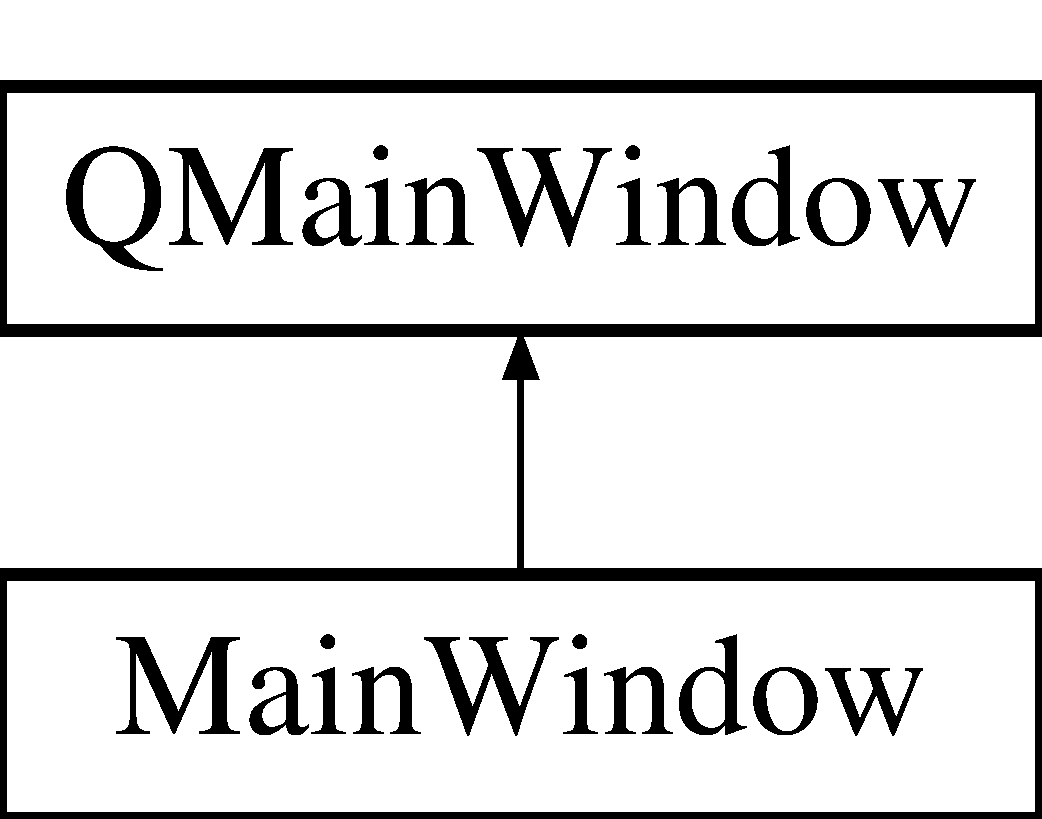
\includegraphics[height=2.000000cm]{class_main_window}
\end{center}
\end{figure}
\subsection*{Public Member Functions}
\begin{DoxyCompactItemize}
\item 
\hyperlink{class_main_window_a8b244be8b7b7db1b08de2a2acb9409db}{Main\+Window} (Q\+Widget $\ast$parent=0)
\begin{DoxyCompactList}\small\item\em \hyperlink{class_main_window_a8b244be8b7b7db1b08de2a2acb9409db}{Main\+Window\+::\+Main\+Window} Constructs the \hyperlink{class_main_window}{Main\+Window} object. Initializes all variables it needs to. By convention, we initialize values in the constructor rather than in the header/declaraton. \end{DoxyCompactList}\item 
\hyperlink{class_main_window_ae98d00a93bc118200eeef9f9bba1dba7}{$\sim$\+Main\+Window} ()
\begin{DoxyCompactList}\small\item\em \hyperlink{class_main_window_ae98d00a93bc118200eeef9f9bba1dba7}{Main\+Window\+::$\sim$\+Main\+Window} The destructor. \end{DoxyCompactList}\end{DoxyCompactItemize}
\subsection*{Public Attributes}
\begin{DoxyCompactItemize}
\item 
Q\+Media\+Player $\ast$ \hyperlink{class_main_window_ab1b0abac053ed137235ee5d4b205a107}{goplayer}
\item 
Q\+Media\+Player $\ast$ \hyperlink{class_main_window_a3c60004c5faa4c7a29b81eb2723d36b9}{stopplayer}
\item 
\hyperlink{class_recording_operation}{Recording\+Operation} $\ast$ \hyperlink{class_main_window_ad5624c21fd77dfdb33d4a7320b6a4ab6}{recording}
\item 
Q\+Timer $\ast$ \hyperlink{class_main_window_afa18558be9a3153936f12dfcdc0e6d8e}{flywheel\+Refresh\+Timer}
\item 
Q\+Timer $\ast$ \hyperlink{class_main_window_aaeb4288152c50a071e0c4df3e1baba85}{graph\+Refresh\+Timer}
\item 
Q\+Timer $\ast$ \hyperlink{class_main_window_abce15ec85ee2078bbb147d081e0a098b}{velocity\+Slope\+Timer}
\item 
Q\+Timer $\ast$ \hyperlink{class_main_window_a61e3faf86f0c2bd56921aacdd4e64c68}{acceleration\+Slope\+Timer}
\item 
bool \hyperlink{class_main_window_a034e18132b1729fa204f92305fb5e71f}{play\+Sounds}
\item 
bool \hyperlink{class_main_window_a23fa0be440d34e4569d9e2d323410e7d}{is\+Recording}
\item 
bool \hyperlink{class_main_window_a1f43f19e84b444053fd775d25d2aa07d}{is\+Scale\+Locked}
\item 
double \hyperlink{class_main_window_aa2c569cb70d25d85e43499d4dca2154b}{graph\+Refresh\+Rate}
\item 
double \hyperlink{class_main_window_ad450b124c5daea75470bb6550081011e}{flywheel\+Refresh\+Rate}
\item 
double \hyperlink{class_main_window_a468f6a2dee29d0488aa82f7e2583b5ae}{target\+Velocity}
\item 
double \hyperlink{class_main_window_a879db4d65600c3b3945d67976d9a8622}{current\+Expected\+Velocity}
\item 
double \hyperlink{class_main_window_a585bfd03f54d4e1f15109de662806090}{target\+Acceleration}
\item 
double \hyperlink{class_main_window_a6382bf386001d617cd5b717a92c5004d}{current\+Expected\+Acceleration}
\item 
double \hyperlink{class_main_window_a380cbb9e901211a3c8fc685cea11c8f9}{current\+Expected\+Jerk}
\item 
double \hyperlink{class_main_window_a1f9fdf363545300d34f5aee2dddb1ff5}{y\+Axis\+Display\+Buffer}
\item 
int \hyperlink{class_main_window_a14e66dcaf2393eed660d558651b07e94}{maximum\+Velocity}
\item 
int \hyperlink{class_main_window_a6b3e09f92d0e995e5c349d6658121364}{maximum\+Acceleration}
\item 
int \hyperlink{class_main_window_a304d68be05ae4cd7086236120933ebcd}{slider\+Tick\+Interval}
\item 
Q\+Key\+Sequence \hyperlink{class_main_window_ad869af059f93289fa358e55d881d20a0}{e\+Stop\+Key}
\item 
Q\+Elapsed\+Timer \hyperlink{class_main_window_af999866626ad70973845e180fe7666f8}{uptime}
\item 
Q\+Action $\ast$ \hyperlink{class_main_window_a0efaeedddca035b6a26ebf229b4ce6ae}{e\+Stop\+Shortcut}
\item 
Ui\+::\+Main\+Window $\ast$ \hyperlink{class_main_window_a35466a70ed47252a0191168126a352a5}{ui}
\end{DoxyCompactItemize}


\subsection{Detailed Description}
The \hyperlink{class_main_window}{Main\+Window} class Comprises the bulk of the G\+UI. 

\subsection{Constructor \& Destructor Documentation}
\hypertarget{class_main_window_a8b244be8b7b7db1b08de2a2acb9409db}{}\label{class_main_window_a8b244be8b7b7db1b08de2a2acb9409db} 
\index{Main\+Window@{Main\+Window}!Main\+Window@{Main\+Window}}
\index{Main\+Window@{Main\+Window}!Main\+Window@{Main\+Window}}
\subsubsection{\texorpdfstring{Main\+Window()}{MainWindow()}}
{\footnotesize\ttfamily Main\+Window\+::\+Main\+Window (\begin{DoxyParamCaption}\item[{Q\+Widget $\ast$}]{parent = {\ttfamily 0} }\end{DoxyParamCaption})\hspace{0.3cm}{\ttfamily [explicit]}}



\hyperlink{class_main_window_a8b244be8b7b7db1b08de2a2acb9409db}{Main\+Window\+::\+Main\+Window} Constructs the \hyperlink{class_main_window}{Main\+Window} object. Initializes all variables it needs to. By convention, we initialize values in the constructor rather than in the header/declaraton. 


\begin{DoxyParams}{Parameters}
{\em parent} & \\
\hline
\end{DoxyParams}
\hypertarget{class_main_window_ae98d00a93bc118200eeef9f9bba1dba7}{}\label{class_main_window_ae98d00a93bc118200eeef9f9bba1dba7} 
\index{Main\+Window@{Main\+Window}!````~Main\+Window@{$\sim$\+Main\+Window}}
\index{````~Main\+Window@{$\sim$\+Main\+Window}!Main\+Window@{Main\+Window}}
\subsubsection{\texorpdfstring{$\sim$\+Main\+Window()}{~MainWindow()}}
{\footnotesize\ttfamily Main\+Window\+::$\sim$\+Main\+Window (\begin{DoxyParamCaption}{ }\end{DoxyParamCaption})}



\hyperlink{class_main_window_ae98d00a93bc118200eeef9f9bba1dba7}{Main\+Window\+::$\sim$\+Main\+Window} The destructor. 



\subsection{Member Data Documentation}
\hypertarget{class_main_window_a61e3faf86f0c2bd56921aacdd4e64c68}{}\label{class_main_window_a61e3faf86f0c2bd56921aacdd4e64c68} 
\index{Main\+Window@{Main\+Window}!acceleration\+Slope\+Timer@{acceleration\+Slope\+Timer}}
\index{acceleration\+Slope\+Timer@{acceleration\+Slope\+Timer}!Main\+Window@{Main\+Window}}
\subsubsection{\texorpdfstring{acceleration\+Slope\+Timer}{accelerationSlopeTimer}}
{\footnotesize\ttfamily Q\+Timer$\ast$ Main\+Window\+::acceleration\+Slope\+Timer}

\hypertarget{class_main_window_a6382bf386001d617cd5b717a92c5004d}{}\label{class_main_window_a6382bf386001d617cd5b717a92c5004d} 
\index{Main\+Window@{Main\+Window}!current\+Expected\+Acceleration@{current\+Expected\+Acceleration}}
\index{current\+Expected\+Acceleration@{current\+Expected\+Acceleration}!Main\+Window@{Main\+Window}}
\subsubsection{\texorpdfstring{current\+Expected\+Acceleration}{currentExpectedAcceleration}}
{\footnotesize\ttfamily double Main\+Window\+::current\+Expected\+Acceleration}

\hypertarget{class_main_window_a380cbb9e901211a3c8fc685cea11c8f9}{}\label{class_main_window_a380cbb9e901211a3c8fc685cea11c8f9} 
\index{Main\+Window@{Main\+Window}!current\+Expected\+Jerk@{current\+Expected\+Jerk}}
\index{current\+Expected\+Jerk@{current\+Expected\+Jerk}!Main\+Window@{Main\+Window}}
\subsubsection{\texorpdfstring{current\+Expected\+Jerk}{currentExpectedJerk}}
{\footnotesize\ttfamily double Main\+Window\+::current\+Expected\+Jerk}

\hypertarget{class_main_window_a879db4d65600c3b3945d67976d9a8622}{}\label{class_main_window_a879db4d65600c3b3945d67976d9a8622} 
\index{Main\+Window@{Main\+Window}!current\+Expected\+Velocity@{current\+Expected\+Velocity}}
\index{current\+Expected\+Velocity@{current\+Expected\+Velocity}!Main\+Window@{Main\+Window}}
\subsubsection{\texorpdfstring{current\+Expected\+Velocity}{currentExpectedVelocity}}
{\footnotesize\ttfamily double Main\+Window\+::current\+Expected\+Velocity}

\hypertarget{class_main_window_ad869af059f93289fa358e55d881d20a0}{}\label{class_main_window_ad869af059f93289fa358e55d881d20a0} 
\index{Main\+Window@{Main\+Window}!e\+Stop\+Key@{e\+Stop\+Key}}
\index{e\+Stop\+Key@{e\+Stop\+Key}!Main\+Window@{Main\+Window}}
\subsubsection{\texorpdfstring{e\+Stop\+Key}{eStopKey}}
{\footnotesize\ttfamily Q\+Key\+Sequence Main\+Window\+::e\+Stop\+Key}

\hypertarget{class_main_window_a0efaeedddca035b6a26ebf229b4ce6ae}{}\label{class_main_window_a0efaeedddca035b6a26ebf229b4ce6ae} 
\index{Main\+Window@{Main\+Window}!e\+Stop\+Shortcut@{e\+Stop\+Shortcut}}
\index{e\+Stop\+Shortcut@{e\+Stop\+Shortcut}!Main\+Window@{Main\+Window}}
\subsubsection{\texorpdfstring{e\+Stop\+Shortcut}{eStopShortcut}}
{\footnotesize\ttfamily Q\+Action$\ast$ Main\+Window\+::e\+Stop\+Shortcut}

\hypertarget{class_main_window_ad450b124c5daea75470bb6550081011e}{}\label{class_main_window_ad450b124c5daea75470bb6550081011e} 
\index{Main\+Window@{Main\+Window}!flywheel\+Refresh\+Rate@{flywheel\+Refresh\+Rate}}
\index{flywheel\+Refresh\+Rate@{flywheel\+Refresh\+Rate}!Main\+Window@{Main\+Window}}
\subsubsection{\texorpdfstring{flywheel\+Refresh\+Rate}{flywheelRefreshRate}}
{\footnotesize\ttfamily double Main\+Window\+::flywheel\+Refresh\+Rate}

\hypertarget{class_main_window_afa18558be9a3153936f12dfcdc0e6d8e}{}\label{class_main_window_afa18558be9a3153936f12dfcdc0e6d8e} 
\index{Main\+Window@{Main\+Window}!flywheel\+Refresh\+Timer@{flywheel\+Refresh\+Timer}}
\index{flywheel\+Refresh\+Timer@{flywheel\+Refresh\+Timer}!Main\+Window@{Main\+Window}}
\subsubsection{\texorpdfstring{flywheel\+Refresh\+Timer}{flywheelRefreshTimer}}
{\footnotesize\ttfamily Q\+Timer$\ast$ Main\+Window\+::flywheel\+Refresh\+Timer}

\hypertarget{class_main_window_ab1b0abac053ed137235ee5d4b205a107}{}\label{class_main_window_ab1b0abac053ed137235ee5d4b205a107} 
\index{Main\+Window@{Main\+Window}!goplayer@{goplayer}}
\index{goplayer@{goplayer}!Main\+Window@{Main\+Window}}
\subsubsection{\texorpdfstring{goplayer}{goplayer}}
{\footnotesize\ttfamily Q\+Media\+Player$\ast$ Main\+Window\+::goplayer}

\hypertarget{class_main_window_aa2c569cb70d25d85e43499d4dca2154b}{}\label{class_main_window_aa2c569cb70d25d85e43499d4dca2154b} 
\index{Main\+Window@{Main\+Window}!graph\+Refresh\+Rate@{graph\+Refresh\+Rate}}
\index{graph\+Refresh\+Rate@{graph\+Refresh\+Rate}!Main\+Window@{Main\+Window}}
\subsubsection{\texorpdfstring{graph\+Refresh\+Rate}{graphRefreshRate}}
{\footnotesize\ttfamily double Main\+Window\+::graph\+Refresh\+Rate}

\hypertarget{class_main_window_aaeb4288152c50a071e0c4df3e1baba85}{}\label{class_main_window_aaeb4288152c50a071e0c4df3e1baba85} 
\index{Main\+Window@{Main\+Window}!graph\+Refresh\+Timer@{graph\+Refresh\+Timer}}
\index{graph\+Refresh\+Timer@{graph\+Refresh\+Timer}!Main\+Window@{Main\+Window}}
\subsubsection{\texorpdfstring{graph\+Refresh\+Timer}{graphRefreshTimer}}
{\footnotesize\ttfamily Q\+Timer$\ast$ Main\+Window\+::graph\+Refresh\+Timer}

\hypertarget{class_main_window_a23fa0be440d34e4569d9e2d323410e7d}{}\label{class_main_window_a23fa0be440d34e4569d9e2d323410e7d} 
\index{Main\+Window@{Main\+Window}!is\+Recording@{is\+Recording}}
\index{is\+Recording@{is\+Recording}!Main\+Window@{Main\+Window}}
\subsubsection{\texorpdfstring{is\+Recording}{isRecording}}
{\footnotesize\ttfamily bool Main\+Window\+::is\+Recording}

\hypertarget{class_main_window_a1f43f19e84b444053fd775d25d2aa07d}{}\label{class_main_window_a1f43f19e84b444053fd775d25d2aa07d} 
\index{Main\+Window@{Main\+Window}!is\+Scale\+Locked@{is\+Scale\+Locked}}
\index{is\+Scale\+Locked@{is\+Scale\+Locked}!Main\+Window@{Main\+Window}}
\subsubsection{\texorpdfstring{is\+Scale\+Locked}{isScaleLocked}}
{\footnotesize\ttfamily bool Main\+Window\+::is\+Scale\+Locked}

\hypertarget{class_main_window_a6b3e09f92d0e995e5c349d6658121364}{}\label{class_main_window_a6b3e09f92d0e995e5c349d6658121364} 
\index{Main\+Window@{Main\+Window}!maximum\+Acceleration@{maximum\+Acceleration}}
\index{maximum\+Acceleration@{maximum\+Acceleration}!Main\+Window@{Main\+Window}}
\subsubsection{\texorpdfstring{maximum\+Acceleration}{maximumAcceleration}}
{\footnotesize\ttfamily int Main\+Window\+::maximum\+Acceleration}

\hypertarget{class_main_window_a14e66dcaf2393eed660d558651b07e94}{}\label{class_main_window_a14e66dcaf2393eed660d558651b07e94} 
\index{Main\+Window@{Main\+Window}!maximum\+Velocity@{maximum\+Velocity}}
\index{maximum\+Velocity@{maximum\+Velocity}!Main\+Window@{Main\+Window}}
\subsubsection{\texorpdfstring{maximum\+Velocity}{maximumVelocity}}
{\footnotesize\ttfamily int Main\+Window\+::maximum\+Velocity}

\hypertarget{class_main_window_a034e18132b1729fa204f92305fb5e71f}{}\label{class_main_window_a034e18132b1729fa204f92305fb5e71f} 
\index{Main\+Window@{Main\+Window}!play\+Sounds@{play\+Sounds}}
\index{play\+Sounds@{play\+Sounds}!Main\+Window@{Main\+Window}}
\subsubsection{\texorpdfstring{play\+Sounds}{playSounds}}
{\footnotesize\ttfamily bool Main\+Window\+::play\+Sounds}

\hypertarget{class_main_window_ad5624c21fd77dfdb33d4a7320b6a4ab6}{}\label{class_main_window_ad5624c21fd77dfdb33d4a7320b6a4ab6} 
\index{Main\+Window@{Main\+Window}!recording@{recording}}
\index{recording@{recording}!Main\+Window@{Main\+Window}}
\subsubsection{\texorpdfstring{recording}{recording}}
{\footnotesize\ttfamily \hyperlink{class_recording_operation}{Recording\+Operation}$\ast$ Main\+Window\+::recording}

\hypertarget{class_main_window_a304d68be05ae4cd7086236120933ebcd}{}\label{class_main_window_a304d68be05ae4cd7086236120933ebcd} 
\index{Main\+Window@{Main\+Window}!slider\+Tick\+Interval@{slider\+Tick\+Interval}}
\index{slider\+Tick\+Interval@{slider\+Tick\+Interval}!Main\+Window@{Main\+Window}}
\subsubsection{\texorpdfstring{slider\+Tick\+Interval}{sliderTickInterval}}
{\footnotesize\ttfamily int Main\+Window\+::slider\+Tick\+Interval}

\hypertarget{class_main_window_a3c60004c5faa4c7a29b81eb2723d36b9}{}\label{class_main_window_a3c60004c5faa4c7a29b81eb2723d36b9} 
\index{Main\+Window@{Main\+Window}!stopplayer@{stopplayer}}
\index{stopplayer@{stopplayer}!Main\+Window@{Main\+Window}}
\subsubsection{\texorpdfstring{stopplayer}{stopplayer}}
{\footnotesize\ttfamily Q\+Media\+Player$\ast$ Main\+Window\+::stopplayer}

\hypertarget{class_main_window_a585bfd03f54d4e1f15109de662806090}{}\label{class_main_window_a585bfd03f54d4e1f15109de662806090} 
\index{Main\+Window@{Main\+Window}!target\+Acceleration@{target\+Acceleration}}
\index{target\+Acceleration@{target\+Acceleration}!Main\+Window@{Main\+Window}}
\subsubsection{\texorpdfstring{target\+Acceleration}{targetAcceleration}}
{\footnotesize\ttfamily double Main\+Window\+::target\+Acceleration}

\hypertarget{class_main_window_a468f6a2dee29d0488aa82f7e2583b5ae}{}\label{class_main_window_a468f6a2dee29d0488aa82f7e2583b5ae} 
\index{Main\+Window@{Main\+Window}!target\+Velocity@{target\+Velocity}}
\index{target\+Velocity@{target\+Velocity}!Main\+Window@{Main\+Window}}
\subsubsection{\texorpdfstring{target\+Velocity}{targetVelocity}}
{\footnotesize\ttfamily double Main\+Window\+::target\+Velocity}

\hypertarget{class_main_window_a35466a70ed47252a0191168126a352a5}{}\label{class_main_window_a35466a70ed47252a0191168126a352a5} 
\index{Main\+Window@{Main\+Window}!ui@{ui}}
\index{ui@{ui}!Main\+Window@{Main\+Window}}
\subsubsection{\texorpdfstring{ui}{ui}}
{\footnotesize\ttfamily Ui\+::\+Main\+Window$\ast$ Main\+Window\+::ui}

\hypertarget{class_main_window_af999866626ad70973845e180fe7666f8}{}\label{class_main_window_af999866626ad70973845e180fe7666f8} 
\index{Main\+Window@{Main\+Window}!uptime@{uptime}}
\index{uptime@{uptime}!Main\+Window@{Main\+Window}}
\subsubsection{\texorpdfstring{uptime}{uptime}}
{\footnotesize\ttfamily Q\+Elapsed\+Timer Main\+Window\+::uptime}

\hypertarget{class_main_window_abce15ec85ee2078bbb147d081e0a098b}{}\label{class_main_window_abce15ec85ee2078bbb147d081e0a098b} 
\index{Main\+Window@{Main\+Window}!velocity\+Slope\+Timer@{velocity\+Slope\+Timer}}
\index{velocity\+Slope\+Timer@{velocity\+Slope\+Timer}!Main\+Window@{Main\+Window}}
\subsubsection{\texorpdfstring{velocity\+Slope\+Timer}{velocitySlopeTimer}}
{\footnotesize\ttfamily Q\+Timer$\ast$ Main\+Window\+::velocity\+Slope\+Timer}

\hypertarget{class_main_window_a1f9fdf363545300d34f5aee2dddb1ff5}{}\label{class_main_window_a1f9fdf363545300d34f5aee2dddb1ff5} 
\index{Main\+Window@{Main\+Window}!y\+Axis\+Display\+Buffer@{y\+Axis\+Display\+Buffer}}
\index{y\+Axis\+Display\+Buffer@{y\+Axis\+Display\+Buffer}!Main\+Window@{Main\+Window}}
\subsubsection{\texorpdfstring{y\+Axis\+Display\+Buffer}{yAxisDisplayBuffer}}
{\footnotesize\ttfamily double Main\+Window\+::y\+Axis\+Display\+Buffer}



The documentation for this class was generated from the following files\+:\begin{DoxyCompactItemize}
\item 
F\+E\+S\+S-\/\+G\+U\+I/\hyperlink{mainwindow_8h}{mainwindow.\+h}\item 
F\+E\+S\+S-\/\+G\+U\+I/\hyperlink{mainwindow_8cpp}{mainwindow.\+cpp}\end{DoxyCompactItemize}

\hypertarget{class_q_c_p_abstract_item}{}\section{Q\+C\+P\+Abstract\+Item Class Reference}
\label{class_q_c_p_abstract_item}\index{Q\+C\+P\+Abstract\+Item@{Q\+C\+P\+Abstract\+Item}}


The abstract base class for all items in a plot.  


Inheritance diagram for Q\+C\+P\+Abstract\+Item\+:\begin{figure}[H]
\begin{center}
\leavevmode
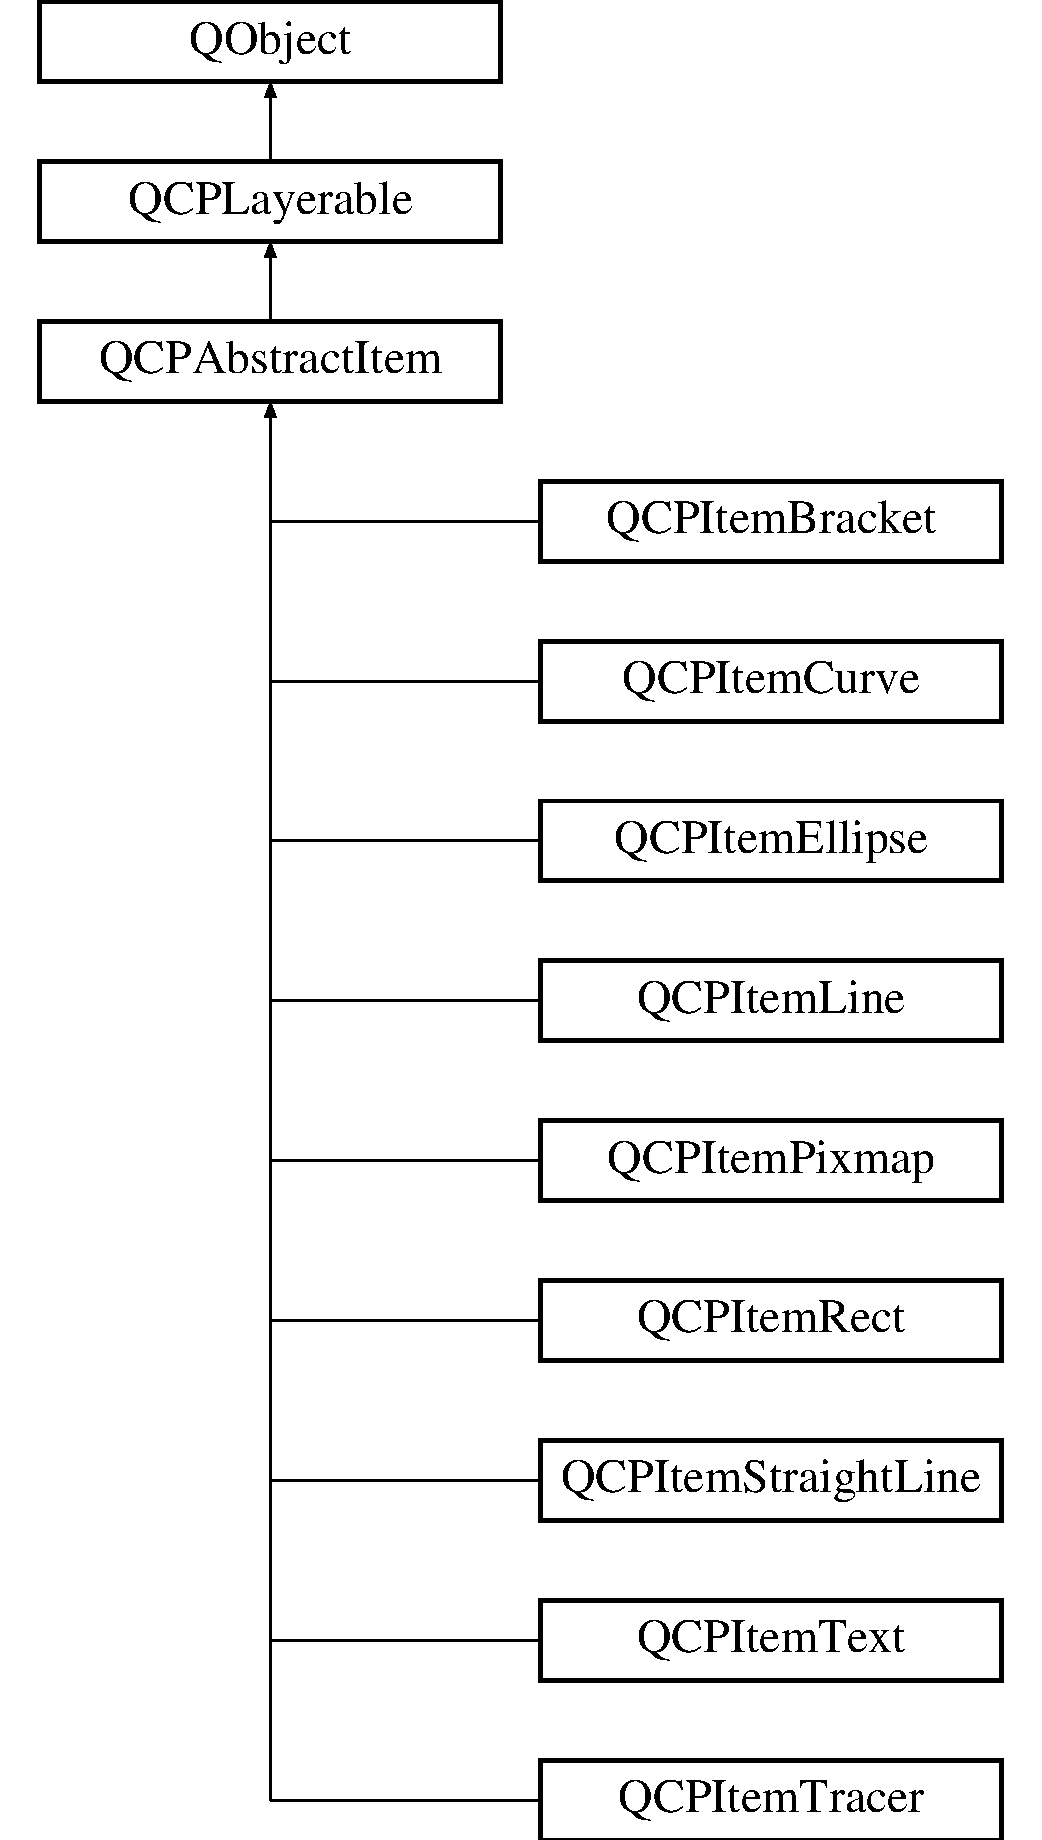
\includegraphics[height=12.000000cm]{class_q_c_p_abstract_item}
\end{center}
\end{figure}
\subsection*{Signals}
\begin{DoxyCompactItemize}
\item 
void \hyperlink{class_q_c_p_abstract_item_aa5cffb034fc65dbb91c77e02c1c14251}{selection\+Changed} (bool selected)
\item 
\hypertarget{class_q_c_p_abstract_item_a5b266c11aac61cb511901f3911dac2a3}{}\label{class_q_c_p_abstract_item_a5b266c11aac61cb511901f3911dac2a3} 
void {\bfseries selectable\+Changed} (bool selectable)
\end{DoxyCompactItemize}
\subsection*{Public Member Functions}
\begin{DoxyCompactItemize}
\item 
\hyperlink{class_q_c_p_abstract_item_a9922507d8b4503a1fe1ed0b1030e23b6}{Q\+C\+P\+Abstract\+Item} (\hyperlink{class_q_custom_plot}{Q\+Custom\+Plot} $\ast$parent\+Plot)
\item 
\hypertarget{class_q_c_p_abstract_item_a42715ad5f3d7fca6854025fa5636f436}{}\label{class_q_c_p_abstract_item_a42715ad5f3d7fca6854025fa5636f436} 
bool {\bfseries clip\+To\+Axis\+Rect} () const
\item 
\hypertarget{class_q_c_p_abstract_item_ae162314efd3fe1a6d4df11da1d275d52}{}\label{class_q_c_p_abstract_item_ae162314efd3fe1a6d4df11da1d275d52} 
\hyperlink{class_q_c_p_axis_rect}{Q\+C\+P\+Axis\+Rect} $\ast$ {\bfseries clip\+Axis\+Rect} () const
\item 
\hypertarget{class_q_c_p_abstract_item_ae29aa489767352b40c4aaa7ea50c5582}{}\label{class_q_c_p_abstract_item_ae29aa489767352b40c4aaa7ea50c5582} 
bool {\bfseries selectable} () const
\item 
\hypertarget{class_q_c_p_abstract_item_aa069fba320a13639f119f82ad29ead96}{}\label{class_q_c_p_abstract_item_aa069fba320a13639f119f82ad29ead96} 
bool {\bfseries selected} () const
\item 
void \hyperlink{class_q_c_p_abstract_item_a39e05b9d4176b9accafc746d16ca6a06}{set\+Clip\+To\+Axis\+Rect} (bool clip)
\item 
void \hyperlink{class_q_c_p_abstract_item_a7dc75fcbcd10206fe0b75d757ea7a347}{set\+Clip\+Axis\+Rect} (\hyperlink{class_q_c_p_axis_rect}{Q\+C\+P\+Axis\+Rect} $\ast$rect)
\item 
Q\+\_\+\+S\+L\+OT void \hyperlink{class_q_c_p_abstract_item_a8a8e32a55bc478b849756a78c2d87fd2}{set\+Selectable} (bool selectable)
\item 
Q\+\_\+\+S\+L\+OT void \hyperlink{class_q_c_p_abstract_item_a203de94ad586cc44d16c9565f49d3378}{set\+Selected} (bool selected)
\item 
virtual double \hyperlink{class_q_c_p_abstract_item_a96d522d10ffc0413b9a366c6f7f0476b}{select\+Test} (const Q\+PointF \&pos, bool only\+Selectable, Q\+Variant $\ast$details=0) const =0
\item 
Q\+List$<$ \hyperlink{class_q_c_p_item_position}{Q\+C\+P\+Item\+Position} $\ast$ $>$ \hyperlink{class_q_c_p_abstract_item_a709f655ac3f7f22d452714134662b454}{positions} () const
\item 
Q\+List$<$ \hyperlink{class_q_c_p_item_anchor}{Q\+C\+P\+Item\+Anchor} $\ast$ $>$ \hyperlink{class_q_c_p_abstract_item_a81d1ecfea3368b836cf9675a0045e659}{anchors} () const
\item 
\hyperlink{class_q_c_p_item_position}{Q\+C\+P\+Item\+Position} $\ast$ \hyperlink{class_q_c_p_abstract_item_a2589c3d298f9a576d77d9addb440a18d}{position} (const Q\+String \&name) const
\item 
\hyperlink{class_q_c_p_item_anchor}{Q\+C\+P\+Item\+Anchor} $\ast$ \hyperlink{class_q_c_p_abstract_item_a139c255ea8831642fac91748e29a5adb}{anchor} (const Q\+String \&name) const
\item 
bool \hyperlink{class_q_c_p_abstract_item_a84914f4516f9b38ef0bd89eafe3dbda7}{has\+Anchor} (const Q\+String \&name) const
\end{DoxyCompactItemize}
\subsection*{Protected Member Functions}
\begin{DoxyCompactItemize}
\item 
\hypertarget{class_q_c_p_abstract_item_a59279d8123663b3b2fffbe54ca075244}{}\label{class_q_c_p_abstract_item_a59279d8123663b3b2fffbe54ca075244} 
virtual \hyperlink{namespace_q_c_p_a2ad6bb6281c7c2d593d4277b44c2b037}{Q\+C\+P\+::\+Interaction} {\bfseries selection\+Category} () const
\item 
\hypertarget{class_q_c_p_abstract_item_a550ecff39195d9ff3d5cf239eb802ea7}{}\label{class_q_c_p_abstract_item_a550ecff39195d9ff3d5cf239eb802ea7} 
virtual Q\+Rect {\bfseries clip\+Rect} () const
\item 
\hypertarget{class_q_c_p_abstract_item_a82a408b38a93be750b934fe847a018cb}{}\label{class_q_c_p_abstract_item_a82a408b38a93be750b934fe847a018cb} 
virtual void {\bfseries apply\+Default\+Antialiasing\+Hint} (\hyperlink{class_q_c_p_painter}{Q\+C\+P\+Painter} $\ast$painter) const
\item 
\hypertarget{class_q_c_p_abstract_item_ad0dc056f650c3ca73414e6b4f01674ef}{}\label{class_q_c_p_abstract_item_ad0dc056f650c3ca73414e6b4f01674ef} 
virtual void {\bfseries draw} (\hyperlink{class_q_c_p_painter}{Q\+C\+P\+Painter} $\ast$painter)=0
\item 
\hypertarget{class_q_c_p_abstract_item_aaf92af7b9893712959a6c073d334d88d}{}\label{class_q_c_p_abstract_item_aaf92af7b9893712959a6c073d334d88d} 
virtual void {\bfseries select\+Event} (Q\+Mouse\+Event $\ast$event, bool additive, const Q\+Variant \&details, bool $\ast$selection\+State\+Changed)
\item 
\hypertarget{class_q_c_p_abstract_item_a91f090d6763cfedb0749219c63788ae9}{}\label{class_q_c_p_abstract_item_a91f090d6763cfedb0749219c63788ae9} 
virtual void {\bfseries deselect\+Event} (bool $\ast$selection\+State\+Changed)
\item 
\hypertarget{class_q_c_p_abstract_item_a5681c190803e899bac9a240753fdba00}{}\label{class_q_c_p_abstract_item_a5681c190803e899bac9a240753fdba00} 
virtual Q\+PointF {\bfseries anchor\+Pixel\+Point} (int anchor\+Id) const
\item 
\hypertarget{class_q_c_p_abstract_item_a8f4d23e883cbb55219959ed6ce8f10ac}{}\label{class_q_c_p_abstract_item_a8f4d23e883cbb55219959ed6ce8f10ac} 
double {\bfseries dist\+Sqr\+To\+Line} (const Q\+PointF \&start, const Q\+PointF \&end, const Q\+PointF \&point) const
\item 
\hypertarget{class_q_c_p_abstract_item_a26aa3828d398e29116afee16216d6b36}{}\label{class_q_c_p_abstract_item_a26aa3828d398e29116afee16216d6b36} 
double {\bfseries rect\+Select\+Test} (const Q\+RectF \&rect, const Q\+PointF \&pos, bool filled\+Rect) const
\item 
\hypertarget{class_q_c_p_abstract_item_a75036d39c4d4e2e1a7dd145fff915d32}{}\label{class_q_c_p_abstract_item_a75036d39c4d4e2e1a7dd145fff915d32} 
\hyperlink{class_q_c_p_item_position}{Q\+C\+P\+Item\+Position} $\ast$ {\bfseries create\+Position} (const Q\+String \&name)
\item 
\hypertarget{class_q_c_p_abstract_item_af3fc92527802078ca395138748b629a7}{}\label{class_q_c_p_abstract_item_af3fc92527802078ca395138748b629a7} 
\hyperlink{class_q_c_p_item_anchor}{Q\+C\+P\+Item\+Anchor} $\ast$ {\bfseries create\+Anchor} (const Q\+String \&name, int anchor\+Id)
\end{DoxyCompactItemize}
\subsection*{Protected Attributes}
\begin{DoxyCompactItemize}
\item 
\hypertarget{class_q_c_p_abstract_item_ad2a70ff6b658fcb84a9427f69d3f587d}{}\label{class_q_c_p_abstract_item_ad2a70ff6b658fcb84a9427f69d3f587d} 
bool {\bfseries m\+Clip\+To\+Axis\+Rect}
\item 
\hypertarget{class_q_c_p_abstract_item_a3e57cfe7da4b1ac3d6fa7281ea437361}{}\label{class_q_c_p_abstract_item_a3e57cfe7da4b1ac3d6fa7281ea437361} 
Q\+Pointer$<$ \hyperlink{class_q_c_p_axis_rect}{Q\+C\+P\+Axis\+Rect} $>$ {\bfseries m\+Clip\+Axis\+Rect}
\item 
\hypertarget{class_q_c_p_abstract_item_af94ff71b6a15ea6d028ab8bd8eccd012}{}\label{class_q_c_p_abstract_item_af94ff71b6a15ea6d028ab8bd8eccd012} 
Q\+List$<$ \hyperlink{class_q_c_p_item_position}{Q\+C\+P\+Item\+Position} $\ast$ $>$ {\bfseries m\+Positions}
\item 
\hypertarget{class_q_c_p_abstract_item_a909a3abab783de302ebf0a0e6f2bbc15}{}\label{class_q_c_p_abstract_item_a909a3abab783de302ebf0a0e6f2bbc15} 
Q\+List$<$ \hyperlink{class_q_c_p_item_anchor}{Q\+C\+P\+Item\+Anchor} $\ast$ $>$ {\bfseries m\+Anchors}
\item 
\hypertarget{class_q_c_p_abstract_item_ad81eb35c8726a0f458db9df9732e0e41}{}\label{class_q_c_p_abstract_item_ad81eb35c8726a0f458db9df9732e0e41} 
bool {\bfseries m\+Selectable}
\item 
\hypertarget{class_q_c_p_abstract_item_a4bdb3457dad1d268c0f78a44152b9645}{}\label{class_q_c_p_abstract_item_a4bdb3457dad1d268c0f78a44152b9645} 
bool {\bfseries m\+Selected}
\end{DoxyCompactItemize}
\subsection*{Friends}
\begin{DoxyCompactItemize}
\item 
\hypertarget{class_q_c_p_abstract_item_a1cdf9df76adcfae45261690aa0ca2198}{}\label{class_q_c_p_abstract_item_a1cdf9df76adcfae45261690aa0ca2198} 
class {\bfseries Q\+Custom\+Plot}
\item 
\hypertarget{class_q_c_p_abstract_item_a61767d414fd57af9eb1741b34268c7fc}{}\label{class_q_c_p_abstract_item_a61767d414fd57af9eb1741b34268c7fc} 
class {\bfseries Q\+C\+P\+Item\+Anchor}
\end{DoxyCompactItemize}


\subsection{Detailed Description}
The abstract base class for all items in a plot. 

In \hyperlink{class_q_custom_plot}{Q\+Custom\+Plot}, items are supplemental graphical elements that are neither plottables (\hyperlink{class_q_c_p_abstract_plottable}{Q\+C\+P\+Abstract\+Plottable}) nor axes (\hyperlink{class_q_c_p_axis}{Q\+C\+P\+Axis}). While plottables are always tied to two axes and thus plot coordinates, items can also be placed in absolute coordinates independent of any axes. Each specific item has at least one \hyperlink{class_q_c_p_item_position}{Q\+C\+P\+Item\+Position} member which controls the positioning. Some items are defined by more than one coordinate and thus have two or more \hyperlink{class_q_c_p_item_position}{Q\+C\+P\+Item\+Position} members (For example, \hyperlink{class_q_c_p_item_rect}{Q\+C\+P\+Item\+Rect} has {\itshape top\+Left} and {\itshape bottom\+Right}).

This abstract base class defines a very basic interface like visibility and clipping. Since this class is abstract, it can\textquotesingle{}t be instantiated. Use one of the subclasses or create a subclass yourself to create new items.

The built-\/in items are\+: \tabulinesep=1mm
\begin{longtabu} spread 0pt [c]{*{2}{|X[-1]}|}
\hline
\hyperlink{class_q_c_p_item_line}{Q\+C\+P\+Item\+Line}&A line defined by a start and an end point. May have different ending styles on each side (e.\+g. arrows). \\\cline{1-2}
\hyperlink{class_q_c_p_item_straight_line}{Q\+C\+P\+Item\+Straight\+Line}&A straight line defined by a start and a direction point. Unlike \hyperlink{class_q_c_p_item_line}{Q\+C\+P\+Item\+Line}, the straight line is infinitely long and has no endings. \\\cline{1-2}
\hyperlink{class_q_c_p_item_curve}{Q\+C\+P\+Item\+Curve}&A curve defined by start, end and two intermediate control points. May have different ending styles on each side (e.\+g. arrows). \\\cline{1-2}
\hyperlink{class_q_c_p_item_rect}{Q\+C\+P\+Item\+Rect}&A rectangle \\\cline{1-2}
\hyperlink{class_q_c_p_item_ellipse}{Q\+C\+P\+Item\+Ellipse}&An ellipse \\\cline{1-2}
\hyperlink{class_q_c_p_item_pixmap}{Q\+C\+P\+Item\+Pixmap}&An arbitrary pixmap \\\cline{1-2}
\hyperlink{class_q_c_p_item_text}{Q\+C\+P\+Item\+Text}&A text label \\\cline{1-2}
\hyperlink{class_q_c_p_item_bracket}{Q\+C\+P\+Item\+Bracket}&A bracket which may be used to reference/highlight certain parts in the plot. \\\cline{1-2}
\hyperlink{class_q_c_p_item_tracer}{Q\+C\+P\+Item\+Tracer}&An item that can be attached to a \hyperlink{class_q_c_p_graph}{Q\+C\+P\+Graph} and sticks to its data points, given a key coordinate. \\\cline{1-2}
\end{longtabu}
\hypertarget{class_q_c_p_abstract_item_items-clipping}{}\subsection{Clipping}\label{class_q_c_p_abstract_item_items-clipping}
Items are by default clipped to the main axis rect (they are only visible inside the axis rect). To make an item visible outside that axis rect, disable clipping via \hyperlink{class_q_c_p_abstract_item_a39e05b9d4176b9accafc746d16ca6a06}{set\+Clip\+To\+Axis\+Rect(false)}.

On the other hand if you want the item to be clipped to a different axis rect, specify it via \hyperlink{class_q_c_p_abstract_item_a7dc75fcbcd10206fe0b75d757ea7a347}{set\+Clip\+Axis\+Rect}. This clip\+Axis\+Rect property of an item is only used for clipping behaviour, and in principle is independent of the coordinate axes the item might be tied to via its position members (\hyperlink{class_q_c_p_item_position_a2185f45c75ac8cb9be89daeaaad50e37}{Q\+C\+P\+Item\+Position\+::set\+Axes}). However, it is common that the axis rect for clipping also contains the axes used for the item positions.\hypertarget{class_q_c_p_abstract_item_items-using}{}\subsection{Using items}\label{class_q_c_p_abstract_item_items-using}
First you instantiate the item you want to use and add it to the plot\+: 
\begin{DoxyCodeInclude}
\end{DoxyCodeInclude}
by default, the positions of the item are bound to the x-\/ and y-\/\+Axis of the plot. So we can just set the plot coordinates where the line should start/end\+: 
\begin{DoxyCodeInclude}
\end{DoxyCodeInclude}
If we don\textquotesingle{}t want the line to be positioned in plot coordinates but a different coordinate system, e.\+g. absolute pixel positions on the \hyperlink{class_q_custom_plot}{Q\+Custom\+Plot} surface, we need to change the position type like this\+: 
\begin{DoxyCodeInclude}
\end{DoxyCodeInclude}
Then we can set the coordinates, this time in pixels\+: 
\begin{DoxyCodeInclude}
\end{DoxyCodeInclude}
and make the line visible on the entire \hyperlink{class_q_custom_plot}{Q\+Custom\+Plot}, by disabling clipping to the axis rect\+: 
\begin{DoxyCodeInclude}
\end{DoxyCodeInclude}
 For more advanced plots, it is even possible to set different types and parent anchors per X/Y coordinate of an item position, using for example \hyperlink{class_q_c_p_item_position_a2113b2351d6d00457fb3559a4e20c3ea}{Q\+C\+P\+Item\+Position\+::set\+TypeX} or \hyperlink{class_q_c_p_item_position_add71461a973927c74e42179480916d9c}{Q\+C\+P\+Item\+Position\+::set\+Parent\+AnchorX}. For details, see the documentation of \hyperlink{class_q_c_p_item_position}{Q\+C\+P\+Item\+Position}.\hypertarget{class_q_c_p_abstract_item_items-subclassing}{}\subsection{Creating own items}\label{class_q_c_p_abstract_item_items-subclassing}
To create an own item, you implement a subclass of \hyperlink{class_q_c_p_abstract_item}{Q\+C\+P\+Abstract\+Item}. These are the pure virtual functions, you must implement\+: \begin{DoxyItemize}
\item \hyperlink{class_q_c_p_abstract_item_a96d522d10ffc0413b9a366c6f7f0476b}{select\+Test} \item draw\end{DoxyItemize}
See the documentation of those functions for what they need to do.\hypertarget{class_q_c_p_abstract_item_items-positioning}{}\subsubsection{Allowing the item to be positioned}\label{class_q_c_p_abstract_item_items-positioning}
As mentioned, item positions are represented by \hyperlink{class_q_c_p_item_position}{Q\+C\+P\+Item\+Position} members. Let\textquotesingle{}s assume the new item shall have only one point as its position (as opposed to two like a rect or multiple like a polygon). You then add a public member of type \hyperlink{class_q_c_p_item_position}{Q\+C\+P\+Item\+Position} like so\+:


\begin{DoxyCode}
\hyperlink{class_q_c_p_item_position}{QCPItemPosition} * \textcolor{keyword}{const} myPosition;
\end{DoxyCode}


the const makes sure the pointer itself can\textquotesingle{}t be modified from the user of your new item (the \hyperlink{class_q_c_p_item_position}{Q\+C\+P\+Item\+Position} instance it points to, can be modified, of course). The initialization of this pointer is made easy with the create\+Position function. Just assign the return value of this function to each \hyperlink{class_q_c_p_item_position}{Q\+C\+P\+Item\+Position} in the constructor of your item. create\+Position takes a string which is the name of the position, typically this is identical to the variable name. For example, the constructor of Q\+C\+P\+Item\+Example could look like this\+:


\begin{DoxyCode}
QCPItemExample::QCPItemExample(\hyperlink{class_q_custom_plot}{QCustomPlot} *parentPlot) :
  \hyperlink{class_q_c_p_abstract_item}{QCPAbstractItem}(parentPlot),
  myPosition(createPosition(\textcolor{stringliteral}{"myPosition"}))
\{
  \textcolor{comment}{// other constructor code}
\}
\end{DoxyCode}
\hypertarget{class_q_c_p_abstract_item_items-drawing}{}\subsubsection{The draw function}\label{class_q_c_p_abstract_item_items-drawing}
To give your item a visual representation, reimplement the draw function and use the passed \hyperlink{class_q_c_p_painter}{Q\+C\+P\+Painter} to draw the item. You can retrieve the item position in pixel coordinates from the position member(s) via \hyperlink{class_q_c_p_item_position_a6cad070c22801295231f5bd6045afe70}{Q\+C\+P\+Item\+Position\+::pixel\+Point}.

To optimize performance you should calculate a bounding rect first (don\textquotesingle{}t forget to take the pen width into account), check whether it intersects the clip\+Rect, and only draw the item at all if this is the case.\hypertarget{class_q_c_p_abstract_item_items-selection}{}\subsubsection{The select\+Test function}\label{class_q_c_p_abstract_item_items-selection}
Your implementation of the \hyperlink{class_q_c_p_abstract_item_a96d522d10ffc0413b9a366c6f7f0476b}{select\+Test} function may use the helpers dist\+Sqr\+To\+Line and rect\+Select\+Test. With these, the implementation of the selection test becomes significantly simpler for most items. See the documentation of \hyperlink{class_q_c_p_abstract_item_a96d522d10ffc0413b9a366c6f7f0476b}{select\+Test} for what the function parameters mean and what the function should return.\hypertarget{class_q_c_p_abstract_item_anchors}{}\subsubsection{Providing anchors}\label{class_q_c_p_abstract_item_anchors}
Providing anchors (\hyperlink{class_q_c_p_item_anchor}{Q\+C\+P\+Item\+Anchor}) starts off like adding a position. First you create a public member, e.\+g.


\begin{DoxyCode}
\hyperlink{class_q_c_p_item_anchor}{QCPItemAnchor} * \textcolor{keyword}{const} bottom;
\end{DoxyCode}


and create it in the constructor with the create\+Anchor function, assigning it a name and an anchor id (an integer enumerating all anchors on the item, you may create an own enum for this). Since anchors can be placed anywhere, relative to the item\textquotesingle{}s position(s), your item needs to provide the position of every anchor with the reimplementation of the anchor\+Pixel\+Point(int anchor\+Id) function.

In essence the \hyperlink{class_q_c_p_item_anchor}{Q\+C\+P\+Item\+Anchor} is merely an intermediary that itself asks your item for the pixel position when anything attached to the anchor needs to know the coordinates. 

\subsection{Constructor \& Destructor Documentation}
\hypertarget{class_q_c_p_abstract_item_a9922507d8b4503a1fe1ed0b1030e23b6}{}\label{class_q_c_p_abstract_item_a9922507d8b4503a1fe1ed0b1030e23b6} 
\index{Q\+C\+P\+Abstract\+Item@{Q\+C\+P\+Abstract\+Item}!Q\+C\+P\+Abstract\+Item@{Q\+C\+P\+Abstract\+Item}}
\index{Q\+C\+P\+Abstract\+Item@{Q\+C\+P\+Abstract\+Item}!Q\+C\+P\+Abstract\+Item@{Q\+C\+P\+Abstract\+Item}}
\subsubsection{\texorpdfstring{Q\+C\+P\+Abstract\+Item()}{QCPAbstractItem()}}
{\footnotesize\ttfamily Q\+C\+P\+Abstract\+Item\+::\+Q\+C\+P\+Abstract\+Item (\begin{DoxyParamCaption}\item[{\hyperlink{class_q_custom_plot}{Q\+Custom\+Plot} $\ast$}]{parent\+Plot }\end{DoxyParamCaption})}

Base class constructor which initializes base class members. 

\subsection{Member Function Documentation}
\hypertarget{class_q_c_p_abstract_item_a139c255ea8831642fac91748e29a5adb}{}\label{class_q_c_p_abstract_item_a139c255ea8831642fac91748e29a5adb} 
\index{Q\+C\+P\+Abstract\+Item@{Q\+C\+P\+Abstract\+Item}!anchor@{anchor}}
\index{anchor@{anchor}!Q\+C\+P\+Abstract\+Item@{Q\+C\+P\+Abstract\+Item}}
\subsubsection{\texorpdfstring{anchor()}{anchor()}}
{\footnotesize\ttfamily \hyperlink{class_q_c_p_item_anchor}{Q\+C\+P\+Item\+Anchor} $\ast$ Q\+C\+P\+Abstract\+Item\+::anchor (\begin{DoxyParamCaption}\item[{const Q\+String \&}]{name }\end{DoxyParamCaption}) const}

Returns the \hyperlink{class_q_c_p_item_anchor}{Q\+C\+P\+Item\+Anchor} with the specified {\itshape name}. If this item doesn\textquotesingle{}t have an anchor by that name, returns 0.

This function provides an alternative way to access item anchors. Normally, you access anchors direcly by their member pointers (which typically have the same variable name as {\itshape name}).

\begin{DoxySeeAlso}{See also}
\hyperlink{class_q_c_p_abstract_item_a81d1ecfea3368b836cf9675a0045e659}{anchors}, \hyperlink{class_q_c_p_abstract_item_a2589c3d298f9a576d77d9addb440a18d}{position} 
\end{DoxySeeAlso}
\hypertarget{class_q_c_p_abstract_item_a81d1ecfea3368b836cf9675a0045e659}{}\label{class_q_c_p_abstract_item_a81d1ecfea3368b836cf9675a0045e659} 
\index{Q\+C\+P\+Abstract\+Item@{Q\+C\+P\+Abstract\+Item}!anchors@{anchors}}
\index{anchors@{anchors}!Q\+C\+P\+Abstract\+Item@{Q\+C\+P\+Abstract\+Item}}
\subsubsection{\texorpdfstring{anchors()}{anchors()}}
{\footnotesize\ttfamily Q\+List$<$ \hyperlink{class_q_c_p_item_anchor}{Q\+C\+P\+Item\+Anchor} $\ast$ $>$ Q\+C\+P\+Abstract\+Item\+::anchors (\begin{DoxyParamCaption}{ }\end{DoxyParamCaption}) const\hspace{0.3cm}{\ttfamily [inline]}}

Returns all anchors of the item in a list. Note that since a position (\hyperlink{class_q_c_p_item_position}{Q\+C\+P\+Item\+Position}) is always also an anchor, the list will also contain the positions of this item.

\begin{DoxySeeAlso}{See also}
\hyperlink{class_q_c_p_abstract_item_a709f655ac3f7f22d452714134662b454}{positions}, \hyperlink{class_q_c_p_abstract_item_a139c255ea8831642fac91748e29a5adb}{anchor} 
\end{DoxySeeAlso}
\hypertarget{class_q_c_p_abstract_item_a84914f4516f9b38ef0bd89eafe3dbda7}{}\label{class_q_c_p_abstract_item_a84914f4516f9b38ef0bd89eafe3dbda7} 
\index{Q\+C\+P\+Abstract\+Item@{Q\+C\+P\+Abstract\+Item}!has\+Anchor@{has\+Anchor}}
\index{has\+Anchor@{has\+Anchor}!Q\+C\+P\+Abstract\+Item@{Q\+C\+P\+Abstract\+Item}}
\subsubsection{\texorpdfstring{has\+Anchor()}{hasAnchor()}}
{\footnotesize\ttfamily bool Q\+C\+P\+Abstract\+Item\+::has\+Anchor (\begin{DoxyParamCaption}\item[{const Q\+String \&}]{name }\end{DoxyParamCaption}) const}

Returns whether this item has an anchor with the specified {\itshape name}.

Note that you can check for positions with this function, too. This is because every position is also an anchor (\hyperlink{class_q_c_p_item_position}{Q\+C\+P\+Item\+Position} inherits from \hyperlink{class_q_c_p_item_anchor}{Q\+C\+P\+Item\+Anchor}).

\begin{DoxySeeAlso}{See also}
\hyperlink{class_q_c_p_abstract_item_a139c255ea8831642fac91748e29a5adb}{anchor}, \hyperlink{class_q_c_p_abstract_item_a2589c3d298f9a576d77d9addb440a18d}{position} 
\end{DoxySeeAlso}
\hypertarget{class_q_c_p_abstract_item_a2589c3d298f9a576d77d9addb440a18d}{}\label{class_q_c_p_abstract_item_a2589c3d298f9a576d77d9addb440a18d} 
\index{Q\+C\+P\+Abstract\+Item@{Q\+C\+P\+Abstract\+Item}!position@{position}}
\index{position@{position}!Q\+C\+P\+Abstract\+Item@{Q\+C\+P\+Abstract\+Item}}
\subsubsection{\texorpdfstring{position()}{position()}}
{\footnotesize\ttfamily \hyperlink{class_q_c_p_item_position}{Q\+C\+P\+Item\+Position} $\ast$ Q\+C\+P\+Abstract\+Item\+::position (\begin{DoxyParamCaption}\item[{const Q\+String \&}]{name }\end{DoxyParamCaption}) const}

Returns the \hyperlink{class_q_c_p_item_position}{Q\+C\+P\+Item\+Position} with the specified {\itshape name}. If this item doesn\textquotesingle{}t have a position by that name, returns 0.

This function provides an alternative way to access item positions. Normally, you access positions direcly by their member pointers (which typically have the same variable name as {\itshape name}).

\begin{DoxySeeAlso}{See also}
\hyperlink{class_q_c_p_abstract_item_a709f655ac3f7f22d452714134662b454}{positions}, \hyperlink{class_q_c_p_abstract_item_a139c255ea8831642fac91748e29a5adb}{anchor} 
\end{DoxySeeAlso}
\hypertarget{class_q_c_p_abstract_item_a709f655ac3f7f22d452714134662b454}{}\label{class_q_c_p_abstract_item_a709f655ac3f7f22d452714134662b454} 
\index{Q\+C\+P\+Abstract\+Item@{Q\+C\+P\+Abstract\+Item}!positions@{positions}}
\index{positions@{positions}!Q\+C\+P\+Abstract\+Item@{Q\+C\+P\+Abstract\+Item}}
\subsubsection{\texorpdfstring{positions()}{positions()}}
{\footnotesize\ttfamily Q\+List$<$ \hyperlink{class_q_c_p_item_position}{Q\+C\+P\+Item\+Position} $\ast$ $>$ Q\+C\+P\+Abstract\+Item\+::positions (\begin{DoxyParamCaption}{ }\end{DoxyParamCaption}) const\hspace{0.3cm}{\ttfamily [inline]}}

Returns all positions of the item in a list.

\begin{DoxySeeAlso}{See also}
\hyperlink{class_q_c_p_abstract_item_a81d1ecfea3368b836cf9675a0045e659}{anchors}, \hyperlink{class_q_c_p_abstract_item_a2589c3d298f9a576d77d9addb440a18d}{position} 
\end{DoxySeeAlso}
\hypertarget{class_q_c_p_abstract_item_aa5cffb034fc65dbb91c77e02c1c14251}{}\label{class_q_c_p_abstract_item_aa5cffb034fc65dbb91c77e02c1c14251} 
\index{Q\+C\+P\+Abstract\+Item@{Q\+C\+P\+Abstract\+Item}!selection\+Changed@{selection\+Changed}}
\index{selection\+Changed@{selection\+Changed}!Q\+C\+P\+Abstract\+Item@{Q\+C\+P\+Abstract\+Item}}
\subsubsection{\texorpdfstring{selection\+Changed}{selectionChanged}}
{\footnotesize\ttfamily void Q\+C\+P\+Abstract\+Item\+::selection\+Changed (\begin{DoxyParamCaption}\item[{bool}]{selected }\end{DoxyParamCaption})\hspace{0.3cm}{\ttfamily [signal]}}

This signal is emitted when the selection state of this item has changed, either by user interaction or by a direct call to \hyperlink{class_q_c_p_abstract_item_a203de94ad586cc44d16c9565f49d3378}{set\+Selected}. \hypertarget{class_q_c_p_abstract_item_a96d522d10ffc0413b9a366c6f7f0476b}{}\label{class_q_c_p_abstract_item_a96d522d10ffc0413b9a366c6f7f0476b} 
\index{Q\+C\+P\+Abstract\+Item@{Q\+C\+P\+Abstract\+Item}!select\+Test@{select\+Test}}
\index{select\+Test@{select\+Test}!Q\+C\+P\+Abstract\+Item@{Q\+C\+P\+Abstract\+Item}}
\subsubsection{\texorpdfstring{select\+Test()}{selectTest()}}
{\footnotesize\ttfamily virtual double Q\+C\+P\+Abstract\+Item\+::select\+Test (\begin{DoxyParamCaption}\item[{const Q\+PointF \&}]{pos,  }\item[{bool}]{only\+Selectable,  }\item[{Q\+Variant $\ast$}]{details = {\ttfamily 0} }\end{DoxyParamCaption}) const\hspace{0.3cm}{\ttfamily [pure virtual]}}

This function is used to decide whether a click hits a layerable object or not.

{\itshape pos} is a point in pixel coordinates on the \hyperlink{class_q_custom_plot}{Q\+Custom\+Plot} surface. This function returns the shortest pixel distance of this point to the object. If the object is either invisible or the distance couldn\textquotesingle{}t be determined, -\/1.\+0 is returned. Further, if {\itshape only\+Selectable} is true and the object is not selectable, -\/1.\+0 is returned, too.

If the object is represented not by single lines but by an area like a \hyperlink{class_q_c_p_item_text}{Q\+C\+P\+Item\+Text} or the bars of a \hyperlink{class_q_c_p_bars}{Q\+C\+P\+Bars} plottable, a click inside the area should also be considered a hit. In these cases this function thus returns a constant value greater zero but still below the parent plot\textquotesingle{}s selection tolerance. (typically the selection\+Tolerance multiplied by 0.\+99).

Providing a constant value for area objects allows selecting line objects even when they are obscured by such area objects, by clicking close to the lines (i.\+e. closer than 0.\+99$\ast$selection\+Tolerance).

The actual setting of the selection state is not done by this function. This is handled by the parent \hyperlink{class_q_custom_plot}{Q\+Custom\+Plot} when the mouse\+Release\+Event occurs, and the finally selected object is notified via the select\+Event/deselect\+Event methods.

{\itshape details} is an optional output parameter. Every layerable subclass may place any information in {\itshape details}. This information will be passed to select\+Event when the parent \hyperlink{class_q_custom_plot}{Q\+Custom\+Plot} decides on the basis of this select\+Test call, that the object was successfully selected. The subsequent call to select\+Event will carry the {\itshape details}. This is useful for multi-\/part objects (like \hyperlink{class_q_c_p_axis}{Q\+C\+P\+Axis}). This way, a possibly complex calculation to decide which part was clicked is only done once in \hyperlink{class_q_c_p_abstract_item_a96d522d10ffc0413b9a366c6f7f0476b}{select\+Test}. The result (i.\+e. the actually clicked part) can then be placed in {\itshape details}. So in the subsequent select\+Event, the decision which part was selected doesn\textquotesingle{}t have to be done a second time for a single selection operation.

You may pass 0 as {\itshape details} to indicate that you are not interested in those selection details.

\begin{DoxySeeAlso}{See also}
select\+Event, deselect\+Event, \hyperlink{class_q_custom_plot_a5ee1e2f6ae27419deca53e75907c27e5}{Q\+Custom\+Plot\+::set\+Interactions} 
\end{DoxySeeAlso}


Reimplemented from \hyperlink{class_q_c_p_layerable_a04db8351fefd44cfdb77958e75c6288e}{Q\+C\+P\+Layerable}.



Implemented in \hyperlink{class_q_c_p_item_bracket_a971299aa6fef75730d6f10efdaf48616}{Q\+C\+P\+Item\+Bracket}, \hyperlink{class_q_c_p_item_tracer_ae1dc728384936184e7552a6d0d67fd75}{Q\+C\+P\+Item\+Tracer}, \hyperlink{class_q_c_p_item_pixmap_a7583a98ebd3f35d2ac5d6c05fad25a6c}{Q\+C\+P\+Item\+Pixmap}, \hyperlink{class_q_c_p_item_ellipse_aa41be2180b2ace2e303b88d005c14243}{Q\+C\+P\+Item\+Ellipse}, \hyperlink{class_q_c_p_item_text_aca74494fd5e769f331a6eb3e29f32916}{Q\+C\+P\+Item\+Text}, \hyperlink{class_q_c_p_item_rect_abe1a6091591d3bad5e4efab2331f99ec}{Q\+C\+P\+Item\+Rect}, \hyperlink{class_q_c_p_item_curve_a8018b8b3fc552a44ba87ca4b64c1523f}{Q\+C\+P\+Item\+Curve}, \hyperlink{class_q_c_p_item_line_ae6cc5183f568e5fa9d7827abe4d405b5}{Q\+C\+P\+Item\+Line}, and \hyperlink{class_q_c_p_item_straight_line_a1e5d99d79efb5871600c72bcd2891a0f}{Q\+C\+P\+Item\+Straight\+Line}.

\hypertarget{class_q_c_p_abstract_item_a7dc75fcbcd10206fe0b75d757ea7a347}{}\label{class_q_c_p_abstract_item_a7dc75fcbcd10206fe0b75d757ea7a347} 
\index{Q\+C\+P\+Abstract\+Item@{Q\+C\+P\+Abstract\+Item}!set\+Clip\+Axis\+Rect@{set\+Clip\+Axis\+Rect}}
\index{set\+Clip\+Axis\+Rect@{set\+Clip\+Axis\+Rect}!Q\+C\+P\+Abstract\+Item@{Q\+C\+P\+Abstract\+Item}}
\subsubsection{\texorpdfstring{set\+Clip\+Axis\+Rect()}{setClipAxisRect()}}
{\footnotesize\ttfamily void Q\+C\+P\+Abstract\+Item\+::set\+Clip\+Axis\+Rect (\begin{DoxyParamCaption}\item[{\hyperlink{class_q_c_p_axis_rect}{Q\+C\+P\+Axis\+Rect} $\ast$}]{rect }\end{DoxyParamCaption})}

Sets the clip axis rect. It defines the rect that will be used to clip the item when \hyperlink{class_q_c_p_abstract_item_a39e05b9d4176b9accafc746d16ca6a06}{set\+Clip\+To\+Axis\+Rect} is set to true.

\begin{DoxySeeAlso}{See also}
\hyperlink{class_q_c_p_abstract_item_a39e05b9d4176b9accafc746d16ca6a06}{set\+Clip\+To\+Axis\+Rect} 
\end{DoxySeeAlso}
\hypertarget{class_q_c_p_abstract_item_a39e05b9d4176b9accafc746d16ca6a06}{}\label{class_q_c_p_abstract_item_a39e05b9d4176b9accafc746d16ca6a06} 
\index{Q\+C\+P\+Abstract\+Item@{Q\+C\+P\+Abstract\+Item}!set\+Clip\+To\+Axis\+Rect@{set\+Clip\+To\+Axis\+Rect}}
\index{set\+Clip\+To\+Axis\+Rect@{set\+Clip\+To\+Axis\+Rect}!Q\+C\+P\+Abstract\+Item@{Q\+C\+P\+Abstract\+Item}}
\subsubsection{\texorpdfstring{set\+Clip\+To\+Axis\+Rect()}{setClipToAxisRect()}}
{\footnotesize\ttfamily void Q\+C\+P\+Abstract\+Item\+::set\+Clip\+To\+Axis\+Rect (\begin{DoxyParamCaption}\item[{bool}]{clip }\end{DoxyParamCaption})}

Sets whether the item shall be clipped to an axis rect or whether it shall be visible on the entire \hyperlink{class_q_custom_plot}{Q\+Custom\+Plot}. The axis rect can be set with \hyperlink{class_q_c_p_abstract_item_a7dc75fcbcd10206fe0b75d757ea7a347}{set\+Clip\+Axis\+Rect}.

\begin{DoxySeeAlso}{See also}
\hyperlink{class_q_c_p_abstract_item_a7dc75fcbcd10206fe0b75d757ea7a347}{set\+Clip\+Axis\+Rect} 
\end{DoxySeeAlso}
\hypertarget{class_q_c_p_abstract_item_a8a8e32a55bc478b849756a78c2d87fd2}{}\label{class_q_c_p_abstract_item_a8a8e32a55bc478b849756a78c2d87fd2} 
\index{Q\+C\+P\+Abstract\+Item@{Q\+C\+P\+Abstract\+Item}!set\+Selectable@{set\+Selectable}}
\index{set\+Selectable@{set\+Selectable}!Q\+C\+P\+Abstract\+Item@{Q\+C\+P\+Abstract\+Item}}
\subsubsection{\texorpdfstring{set\+Selectable()}{setSelectable()}}
{\footnotesize\ttfamily void Q\+C\+P\+Abstract\+Item\+::set\+Selectable (\begin{DoxyParamCaption}\item[{bool}]{selectable }\end{DoxyParamCaption})}

Sets whether the user can (de-\/)select this item by clicking on the \hyperlink{class_q_custom_plot}{Q\+Custom\+Plot} surface. (When \hyperlink{class_q_custom_plot_a5ee1e2f6ae27419deca53e75907c27e5}{Q\+Custom\+Plot\+::set\+Interactions} contains Q\+Custom\+Plot\+::i\+Select\+Items.)

However, even when {\itshape selectable} was set to false, it is possible to set the selection manually, by calling \hyperlink{class_q_c_p_abstract_item_a203de94ad586cc44d16c9565f49d3378}{set\+Selected}.

\begin{DoxySeeAlso}{See also}
\hyperlink{class_q_custom_plot_a5ee1e2f6ae27419deca53e75907c27e5}{Q\+Custom\+Plot\+::set\+Interactions}, \hyperlink{class_q_c_p_abstract_item_a203de94ad586cc44d16c9565f49d3378}{set\+Selected} 
\end{DoxySeeAlso}
\hypertarget{class_q_c_p_abstract_item_a203de94ad586cc44d16c9565f49d3378}{}\label{class_q_c_p_abstract_item_a203de94ad586cc44d16c9565f49d3378} 
\index{Q\+C\+P\+Abstract\+Item@{Q\+C\+P\+Abstract\+Item}!set\+Selected@{set\+Selected}}
\index{set\+Selected@{set\+Selected}!Q\+C\+P\+Abstract\+Item@{Q\+C\+P\+Abstract\+Item}}
\subsubsection{\texorpdfstring{set\+Selected()}{setSelected()}}
{\footnotesize\ttfamily void Q\+C\+P\+Abstract\+Item\+::set\+Selected (\begin{DoxyParamCaption}\item[{bool}]{selected }\end{DoxyParamCaption})}

Sets whether this item is selected or not. When selected, it might use a different visual appearance (e.\+g. pen and brush), this depends on the specific item though.

The entire selection mechanism for items is handled automatically when \hyperlink{class_q_custom_plot_a5ee1e2f6ae27419deca53e75907c27e5}{Q\+Custom\+Plot\+::set\+Interactions} contains Q\+Custom\+Plot\+::i\+Select\+Items. You only need to call this function when you wish to change the selection state manually.

This function can change the selection state even when \hyperlink{class_q_c_p_abstract_item_a8a8e32a55bc478b849756a78c2d87fd2}{set\+Selectable} was set to false.

emits the \hyperlink{class_q_c_p_abstract_item_aa5cffb034fc65dbb91c77e02c1c14251}{selection\+Changed} signal when {\itshape selected} is different from the previous selection state.

\begin{DoxySeeAlso}{See also}
\hyperlink{class_q_c_p_abstract_item_a8a8e32a55bc478b849756a78c2d87fd2}{set\+Selectable}, \hyperlink{class_q_c_p_abstract_item_a96d522d10ffc0413b9a366c6f7f0476b}{select\+Test} 
\end{DoxySeeAlso}


The documentation for this class was generated from the following files\+:\begin{DoxyCompactItemize}
\item 
F\+E\+S\+S-\/\+G\+U\+I/\hyperlink{qcustomplot_8h}{qcustomplot.\+h}\item 
F\+E\+S\+S-\/\+G\+U\+I/\hyperlink{qcustomplot_8cpp}{qcustomplot.\+cpp}\end{DoxyCompactItemize}

\hypertarget{class_q_c_p_abstract_legend_item}{}\section{Q\+C\+P\+Abstract\+Legend\+Item Class Reference}
\label{class_q_c_p_abstract_legend_item}\index{Q\+C\+P\+Abstract\+Legend\+Item@{Q\+C\+P\+Abstract\+Legend\+Item}}


The abstract base class for all entries in a \hyperlink{class_q_c_p_legend}{Q\+C\+P\+Legend}.  


Inheritance diagram for Q\+C\+P\+Abstract\+Legend\+Item\+:\begin{figure}[H]
\begin{center}
\leavevmode
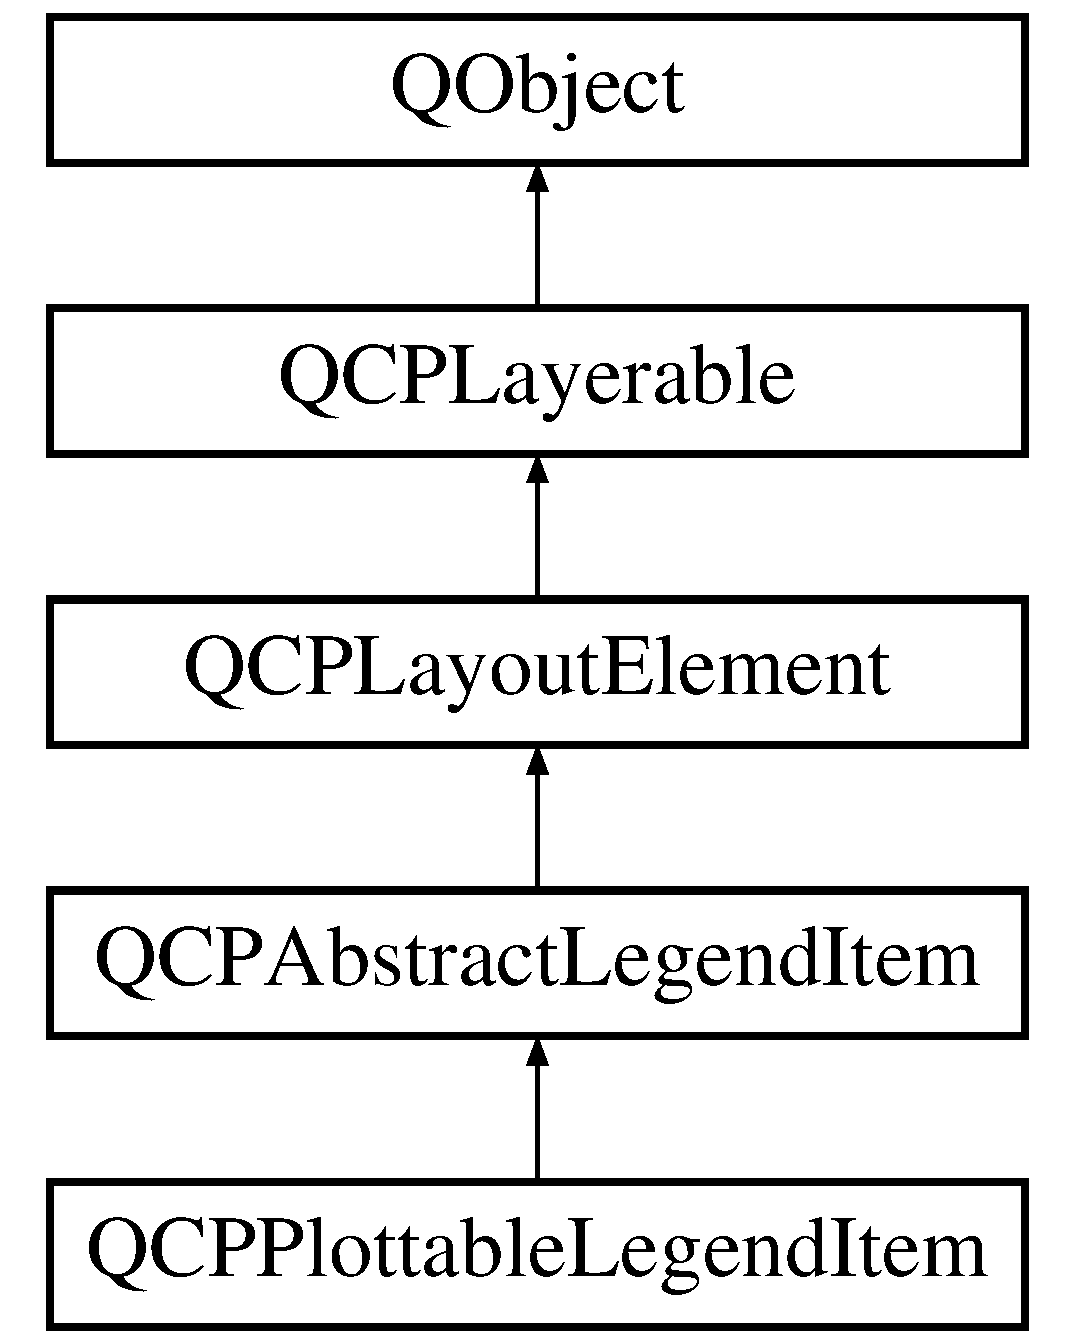
\includegraphics[height=5.000000cm]{class_q_c_p_abstract_legend_item}
\end{center}
\end{figure}
\subsection*{Signals}
\begin{DoxyCompactItemize}
\item 
void \hyperlink{class_q_c_p_abstract_legend_item_a7cb61fdfbaf69c590bacb8f9e7099d9e}{selection\+Changed} (bool selected)
\item 
\hypertarget{class_q_c_p_abstract_legend_item_abc4d779b938cc9235f9196737dbaa6bd}{}\label{class_q_c_p_abstract_legend_item_abc4d779b938cc9235f9196737dbaa6bd} 
void {\bfseries selectable\+Changed} (bool selectable)
\end{DoxyCompactItemize}
\subsection*{Public Member Functions}
\begin{DoxyCompactItemize}
\item 
\hyperlink{class_q_c_p_abstract_legend_item_afaff87610e8da0fa238ecf552872d774}{Q\+C\+P\+Abstract\+Legend\+Item} (\hyperlink{class_q_c_p_legend}{Q\+C\+P\+Legend} $\ast$parent)
\item 
\hypertarget{class_q_c_p_abstract_legend_item_a15709a3f6b2ce3946261fe90422ae32e}{}\label{class_q_c_p_abstract_legend_item_a15709a3f6b2ce3946261fe90422ae32e} 
\hyperlink{class_q_c_p_legend}{Q\+C\+P\+Legend} $\ast$ {\bfseries parent\+Legend} () const
\item 
\hypertarget{class_q_c_p_abstract_legend_item_a699b18e1d9e70372e51e75f462dbb643}{}\label{class_q_c_p_abstract_legend_item_a699b18e1d9e70372e51e75f462dbb643} 
Q\+Font {\bfseries font} () const
\item 
\hypertarget{class_q_c_p_abstract_legend_item_a35b35fa697dcece86cf7e5818c0820b2}{}\label{class_q_c_p_abstract_legend_item_a35b35fa697dcece86cf7e5818c0820b2} 
Q\+Color {\bfseries text\+Color} () const
\item 
\hypertarget{class_q_c_p_abstract_legend_item_ace98814b31762578228f6b32111cd3c0}{}\label{class_q_c_p_abstract_legend_item_ace98814b31762578228f6b32111cd3c0} 
Q\+Font {\bfseries selected\+Font} () const
\item 
\hypertarget{class_q_c_p_abstract_legend_item_a09540594509fb0074f3a1b39548e3bdc}{}\label{class_q_c_p_abstract_legend_item_a09540594509fb0074f3a1b39548e3bdc} 
Q\+Color {\bfseries selected\+Text\+Color} () const
\item 
\hypertarget{class_q_c_p_abstract_legend_item_af054a668038bcd7e35a35a07d1e79a23}{}\label{class_q_c_p_abstract_legend_item_af054a668038bcd7e35a35a07d1e79a23} 
bool {\bfseries selectable} () const
\item 
\hypertarget{class_q_c_p_abstract_legend_item_adf427dbb05d5f1a8e84c6abcb05becdf}{}\label{class_q_c_p_abstract_legend_item_adf427dbb05d5f1a8e84c6abcb05becdf} 
bool {\bfseries selected} () const
\item 
void \hyperlink{class_q_c_p_abstract_legend_item_a409c53455d8112f71d70c0c43eb10265}{set\+Font} (const Q\+Font \&font)
\item 
void \hyperlink{class_q_c_p_abstract_legend_item_a6ebace6aaffaedcdab2d74e88acc2d1e}{set\+Text\+Color} (const Q\+Color \&color)
\item 
void \hyperlink{class_q_c_p_abstract_legend_item_a91db5aee48617a9d3206e61376807365}{set\+Selected\+Font} (const Q\+Font \&font)
\item 
void \hyperlink{class_q_c_p_abstract_legend_item_a4d01d008ee1a5bfe9905b0397a421936}{set\+Selected\+Text\+Color} (const Q\+Color \&color)
\item 
Q\+\_\+\+S\+L\+OT void \hyperlink{class_q_c_p_abstract_legend_item_a9913ef48730551b696e7f98a2391c599}{set\+Selectable} (bool selectable)
\item 
Q\+\_\+\+S\+L\+OT void \hyperlink{class_q_c_p_abstract_legend_item_a6eed93b0ab99cb3eabb043fb08179c2b}{set\+Selected} (bool selected)
\item 
virtual double \hyperlink{class_q_c_p_abstract_legend_item_ac834bf9003c491e5064a31e2a7de418d}{select\+Test} (const Q\+PointF \&pos, bool only\+Selectable, Q\+Variant $\ast$details=0) const
\end{DoxyCompactItemize}
\subsection*{Protected Member Functions}
\begin{DoxyCompactItemize}
\item 
\hypertarget{class_q_c_p_abstract_legend_item_aa8b996ea6b01ee04fff267afffa58135}{}\label{class_q_c_p_abstract_legend_item_aa8b996ea6b01ee04fff267afffa58135} 
virtual \hyperlink{namespace_q_c_p_a2ad6bb6281c7c2d593d4277b44c2b037}{Q\+C\+P\+::\+Interaction} {\bfseries selection\+Category} () const
\item 
\hypertarget{class_q_c_p_abstract_legend_item_a8e69a5e58a526ba0cb2c7619e7ba4da9}{}\label{class_q_c_p_abstract_legend_item_a8e69a5e58a526ba0cb2c7619e7ba4da9} 
virtual void {\bfseries apply\+Default\+Antialiasing\+Hint} (\hyperlink{class_q_c_p_painter}{Q\+C\+P\+Painter} $\ast$painter) const
\item 
\hypertarget{class_q_c_p_abstract_legend_item_ac7880619763e765438da3b4dfe183336}{}\label{class_q_c_p_abstract_legend_item_ac7880619763e765438da3b4dfe183336} 
virtual Q\+Rect {\bfseries clip\+Rect} () const
\item 
\hypertarget{class_q_c_p_abstract_legend_item_a97dedc084c672359710f16b31d046d1d}{}\label{class_q_c_p_abstract_legend_item_a97dedc084c672359710f16b31d046d1d} 
virtual void {\bfseries draw} (\hyperlink{class_q_c_p_painter}{Q\+C\+P\+Painter} $\ast$painter)=0
\item 
\hypertarget{class_q_c_p_abstract_legend_item_abcfe9e335d99c7fac74e03d26723c1b7}{}\label{class_q_c_p_abstract_legend_item_abcfe9e335d99c7fac74e03d26723c1b7} 
virtual void {\bfseries select\+Event} (Q\+Mouse\+Event $\ast$event, bool additive, const Q\+Variant \&details, bool $\ast$selection\+State\+Changed)
\item 
\hypertarget{class_q_c_p_abstract_legend_item_ae64e667e7c5b85cd92c9b91928faef28}{}\label{class_q_c_p_abstract_legend_item_ae64e667e7c5b85cd92c9b91928faef28} 
virtual void {\bfseries deselect\+Event} (bool $\ast$selection\+State\+Changed)
\end{DoxyCompactItemize}
\subsection*{Protected Attributes}
\begin{DoxyCompactItemize}
\item 
\hypertarget{class_q_c_p_abstract_legend_item_aafcd9fc6fcb10f4a8d46037011afafe8}{}\label{class_q_c_p_abstract_legend_item_aafcd9fc6fcb10f4a8d46037011afafe8} 
\hyperlink{class_q_c_p_legend}{Q\+C\+P\+Legend} $\ast$ {\bfseries m\+Parent\+Legend}
\item 
\hypertarget{class_q_c_p_abstract_legend_item_ae916a78ac0d2a60e20a17ca2f24f9754}{}\label{class_q_c_p_abstract_legend_item_ae916a78ac0d2a60e20a17ca2f24f9754} 
Q\+Font {\bfseries m\+Font}
\item 
\hypertarget{class_q_c_p_abstract_legend_item_a974b21e9930227d281344bd2242d289d}{}\label{class_q_c_p_abstract_legend_item_a974b21e9930227d281344bd2242d289d} 
Q\+Color {\bfseries m\+Text\+Color}
\item 
\hypertarget{class_q_c_p_abstract_legend_item_ab971df604306b192875a7d097feb1e21}{}\label{class_q_c_p_abstract_legend_item_ab971df604306b192875a7d097feb1e21} 
Q\+Font {\bfseries m\+Selected\+Font}
\item 
\hypertarget{class_q_c_p_abstract_legend_item_a4965c13854d970b24c284f0a4f005fbd}{}\label{class_q_c_p_abstract_legend_item_a4965c13854d970b24c284f0a4f005fbd} 
Q\+Color {\bfseries m\+Selected\+Text\+Color}
\item 
\hypertarget{class_q_c_p_abstract_legend_item_aa84029f57b1b32f642fb7db63c3fc2c2}{}\label{class_q_c_p_abstract_legend_item_aa84029f57b1b32f642fb7db63c3fc2c2} 
bool {\bfseries m\+Selectable}
\item 
\hypertarget{class_q_c_p_abstract_legend_item_ae58ebebbd0c36cc6fe897483369984d2}{}\label{class_q_c_p_abstract_legend_item_ae58ebebbd0c36cc6fe897483369984d2} 
bool {\bfseries m\+Selected}
\end{DoxyCompactItemize}
\subsection*{Friends}
\begin{DoxyCompactItemize}
\item 
\hypertarget{class_q_c_p_abstract_legend_item_a8429035e7adfbd7f05805a6530ad5e3b}{}\label{class_q_c_p_abstract_legend_item_a8429035e7adfbd7f05805a6530ad5e3b} 
class {\bfseries Q\+C\+P\+Legend}
\end{DoxyCompactItemize}
\subsection*{Additional Inherited Members}


\subsection{Detailed Description}
The abstract base class for all entries in a \hyperlink{class_q_c_p_legend}{Q\+C\+P\+Legend}. 

It defines a very basic interface for entries in a \hyperlink{class_q_c_p_legend}{Q\+C\+P\+Legend}. For representing plottables in the legend, the subclass \hyperlink{class_q_c_p_plottable_legend_item}{Q\+C\+P\+Plottable\+Legend\+Item} is more suitable.

Only derive directly from this class when you need absolute freedom (e.\+g. a custom legend entry that\textquotesingle{}s not even associated with a plottable).

You must implement the following pure virtual functions\+: \begin{DoxyItemize}
\item draw (from \hyperlink{class_q_c_p_layerable}{Q\+C\+P\+Layerable})\end{DoxyItemize}
You inherit the following members you may use\+: \tabulinesep=1mm
\begin{longtabu} spread 0pt [c]{*{2}{|X[-1]}|}
\hline
\hyperlink{class_q_c_p_legend}{Q\+C\+P\+Legend} $\ast${\bfseries m\+Parent\+Legend}  &A pointer to the parent \hyperlink{class_q_c_p_legend}{Q\+C\+P\+Legend}. \\\cline{1-2}
Q\+Font {\bfseries m\+Font}  &The generic font of the item. You should use this font for all or at least the most prominent text of the item.  \\\cline{1-2}
\end{longtabu}


\subsection{Constructor \& Destructor Documentation}
\hypertarget{class_q_c_p_abstract_legend_item_afaff87610e8da0fa238ecf552872d774}{}\label{class_q_c_p_abstract_legend_item_afaff87610e8da0fa238ecf552872d774} 
\index{Q\+C\+P\+Abstract\+Legend\+Item@{Q\+C\+P\+Abstract\+Legend\+Item}!Q\+C\+P\+Abstract\+Legend\+Item@{Q\+C\+P\+Abstract\+Legend\+Item}}
\index{Q\+C\+P\+Abstract\+Legend\+Item@{Q\+C\+P\+Abstract\+Legend\+Item}!Q\+C\+P\+Abstract\+Legend\+Item@{Q\+C\+P\+Abstract\+Legend\+Item}}
\subsubsection{\texorpdfstring{Q\+C\+P\+Abstract\+Legend\+Item()}{QCPAbstractLegendItem()}}
{\footnotesize\ttfamily Q\+C\+P\+Abstract\+Legend\+Item\+::\+Q\+C\+P\+Abstract\+Legend\+Item (\begin{DoxyParamCaption}\item[{\hyperlink{class_q_c_p_legend}{Q\+C\+P\+Legend} $\ast$}]{parent }\end{DoxyParamCaption})\hspace{0.3cm}{\ttfamily [explicit]}}

Constructs a \hyperlink{class_q_c_p_abstract_legend_item}{Q\+C\+P\+Abstract\+Legend\+Item} and associates it with the \hyperlink{class_q_c_p_legend}{Q\+C\+P\+Legend} {\itshape parent}. This does not cause the item to be added to {\itshape parent}, so \hyperlink{class_q_c_p_legend_a3ab274de52d2951faea45a6d975e6b3f}{Q\+C\+P\+Legend\+::add\+Item} must be called separately. 

\subsection{Member Function Documentation}
\hypertarget{class_q_c_p_abstract_legend_item_a7cb61fdfbaf69c590bacb8f9e7099d9e}{}\label{class_q_c_p_abstract_legend_item_a7cb61fdfbaf69c590bacb8f9e7099d9e} 
\index{Q\+C\+P\+Abstract\+Legend\+Item@{Q\+C\+P\+Abstract\+Legend\+Item}!selection\+Changed@{selection\+Changed}}
\index{selection\+Changed@{selection\+Changed}!Q\+C\+P\+Abstract\+Legend\+Item@{Q\+C\+P\+Abstract\+Legend\+Item}}
\subsubsection{\texorpdfstring{selection\+Changed}{selectionChanged}}
{\footnotesize\ttfamily void Q\+C\+P\+Abstract\+Legend\+Item\+::selection\+Changed (\begin{DoxyParamCaption}\item[{bool}]{selected }\end{DoxyParamCaption})\hspace{0.3cm}{\ttfamily [signal]}}

This signal is emitted when the selection state of this legend item has changed, either by user interaction or by a direct call to \hyperlink{class_q_c_p_abstract_legend_item_a6eed93b0ab99cb3eabb043fb08179c2b}{set\+Selected}. \hypertarget{class_q_c_p_abstract_legend_item_ac834bf9003c491e5064a31e2a7de418d}{}\label{class_q_c_p_abstract_legend_item_ac834bf9003c491e5064a31e2a7de418d} 
\index{Q\+C\+P\+Abstract\+Legend\+Item@{Q\+C\+P\+Abstract\+Legend\+Item}!select\+Test@{select\+Test}}
\index{select\+Test@{select\+Test}!Q\+C\+P\+Abstract\+Legend\+Item@{Q\+C\+P\+Abstract\+Legend\+Item}}
\subsubsection{\texorpdfstring{select\+Test()}{selectTest()}}
{\footnotesize\ttfamily double Q\+C\+P\+Abstract\+Legend\+Item\+::select\+Test (\begin{DoxyParamCaption}\item[{const Q\+PointF \&}]{pos,  }\item[{bool}]{only\+Selectable,  }\item[{Q\+Variant $\ast$}]{details = {\ttfamily 0} }\end{DoxyParamCaption}) const\hspace{0.3cm}{\ttfamily [virtual]}}

Layout elements are sensitive to events inside their outer rect. If {\itshape pos} is within the outer rect, this method returns a value corresponding to 0.\+99 times the parent plot\textquotesingle{}s selection tolerance. However, layout elements are not selectable by default. So if {\itshape only\+Selectable} is true, -\/1.\+0 is returned.

See \hyperlink{class_q_c_p_layerable_a04db8351fefd44cfdb77958e75c6288e}{Q\+C\+P\+Layerable\+::select\+Test} for a general explanation of this virtual method.

\hyperlink{class_q_c_p_layout_element}{Q\+C\+P\+Layout\+Element} subclasses may reimplement this method to provide more specific selection test behaviour. 

Reimplemented from \hyperlink{class_q_c_p_layout_element_a0b96ae0d7bcfa6e38188fcb1e73e143f}{Q\+C\+P\+Layout\+Element}.

\hypertarget{class_q_c_p_abstract_legend_item_a409c53455d8112f71d70c0c43eb10265}{}\label{class_q_c_p_abstract_legend_item_a409c53455d8112f71d70c0c43eb10265} 
\index{Q\+C\+P\+Abstract\+Legend\+Item@{Q\+C\+P\+Abstract\+Legend\+Item}!set\+Font@{set\+Font}}
\index{set\+Font@{set\+Font}!Q\+C\+P\+Abstract\+Legend\+Item@{Q\+C\+P\+Abstract\+Legend\+Item}}
\subsubsection{\texorpdfstring{set\+Font()}{setFont()}}
{\footnotesize\ttfamily void Q\+C\+P\+Abstract\+Legend\+Item\+::set\+Font (\begin{DoxyParamCaption}\item[{const Q\+Font \&}]{font }\end{DoxyParamCaption})}

Sets the default font of this specific legend item to {\itshape font}.

\begin{DoxySeeAlso}{See also}
\hyperlink{class_q_c_p_abstract_legend_item_a6ebace6aaffaedcdab2d74e88acc2d1e}{set\+Text\+Color}, \hyperlink{class_q_c_p_legend_aa4cda8499e3cb0f3be415edc02984c73}{Q\+C\+P\+Legend\+::set\+Font} 
\end{DoxySeeAlso}
\hypertarget{class_q_c_p_abstract_legend_item_a9913ef48730551b696e7f98a2391c599}{}\label{class_q_c_p_abstract_legend_item_a9913ef48730551b696e7f98a2391c599} 
\index{Q\+C\+P\+Abstract\+Legend\+Item@{Q\+C\+P\+Abstract\+Legend\+Item}!set\+Selectable@{set\+Selectable}}
\index{set\+Selectable@{set\+Selectable}!Q\+C\+P\+Abstract\+Legend\+Item@{Q\+C\+P\+Abstract\+Legend\+Item}}
\subsubsection{\texorpdfstring{set\+Selectable()}{setSelectable()}}
{\footnotesize\ttfamily void Q\+C\+P\+Abstract\+Legend\+Item\+::set\+Selectable (\begin{DoxyParamCaption}\item[{bool}]{selectable }\end{DoxyParamCaption})}

Sets whether this specific legend item is selectable.

\begin{DoxySeeAlso}{See also}
set\+Selected\+Parts, \hyperlink{class_q_custom_plot_a5ee1e2f6ae27419deca53e75907c27e5}{Q\+Custom\+Plot\+::set\+Interactions} 
\end{DoxySeeAlso}
\hypertarget{class_q_c_p_abstract_legend_item_a6eed93b0ab99cb3eabb043fb08179c2b}{}\label{class_q_c_p_abstract_legend_item_a6eed93b0ab99cb3eabb043fb08179c2b} 
\index{Q\+C\+P\+Abstract\+Legend\+Item@{Q\+C\+P\+Abstract\+Legend\+Item}!set\+Selected@{set\+Selected}}
\index{set\+Selected@{set\+Selected}!Q\+C\+P\+Abstract\+Legend\+Item@{Q\+C\+P\+Abstract\+Legend\+Item}}
\subsubsection{\texorpdfstring{set\+Selected()}{setSelected()}}
{\footnotesize\ttfamily void Q\+C\+P\+Abstract\+Legend\+Item\+::set\+Selected (\begin{DoxyParamCaption}\item[{bool}]{selected }\end{DoxyParamCaption})}

Sets whether this specific legend item is selected.

It is possible to set the selection state of this item by calling this function directly, even if set\+Selectable is set to false.

\begin{DoxySeeAlso}{See also}
set\+Selectable\+Parts, \hyperlink{class_q_custom_plot_a5ee1e2f6ae27419deca53e75907c27e5}{Q\+Custom\+Plot\+::set\+Interactions} 
\end{DoxySeeAlso}
\hypertarget{class_q_c_p_abstract_legend_item_a91db5aee48617a9d3206e61376807365}{}\label{class_q_c_p_abstract_legend_item_a91db5aee48617a9d3206e61376807365} 
\index{Q\+C\+P\+Abstract\+Legend\+Item@{Q\+C\+P\+Abstract\+Legend\+Item}!set\+Selected\+Font@{set\+Selected\+Font}}
\index{set\+Selected\+Font@{set\+Selected\+Font}!Q\+C\+P\+Abstract\+Legend\+Item@{Q\+C\+P\+Abstract\+Legend\+Item}}
\subsubsection{\texorpdfstring{set\+Selected\+Font()}{setSelectedFont()}}
{\footnotesize\ttfamily void Q\+C\+P\+Abstract\+Legend\+Item\+::set\+Selected\+Font (\begin{DoxyParamCaption}\item[{const Q\+Font \&}]{font }\end{DoxyParamCaption})}

When this legend item is selected, {\itshape font} is used to draw generic text, instead of the normal font set with \hyperlink{class_q_c_p_abstract_legend_item_a409c53455d8112f71d70c0c43eb10265}{set\+Font}.

\begin{DoxySeeAlso}{See also}
\hyperlink{class_q_c_p_abstract_legend_item_a409c53455d8112f71d70c0c43eb10265}{set\+Font}, \hyperlink{class_q_c_p_legend_ab580a01c3c0a239374ed66c29edf5ad2}{Q\+C\+P\+Legend\+::set\+Selected\+Font} 
\end{DoxySeeAlso}
\hypertarget{class_q_c_p_abstract_legend_item_a4d01d008ee1a5bfe9905b0397a421936}{}\label{class_q_c_p_abstract_legend_item_a4d01d008ee1a5bfe9905b0397a421936} 
\index{Q\+C\+P\+Abstract\+Legend\+Item@{Q\+C\+P\+Abstract\+Legend\+Item}!set\+Selected\+Text\+Color@{set\+Selected\+Text\+Color}}
\index{set\+Selected\+Text\+Color@{set\+Selected\+Text\+Color}!Q\+C\+P\+Abstract\+Legend\+Item@{Q\+C\+P\+Abstract\+Legend\+Item}}
\subsubsection{\texorpdfstring{set\+Selected\+Text\+Color()}{setSelectedTextColor()}}
{\footnotesize\ttfamily void Q\+C\+P\+Abstract\+Legend\+Item\+::set\+Selected\+Text\+Color (\begin{DoxyParamCaption}\item[{const Q\+Color \&}]{color }\end{DoxyParamCaption})}

When this legend item is selected, {\itshape color} is used to draw generic text, instead of the normal color set with \hyperlink{class_q_c_p_abstract_legend_item_a6ebace6aaffaedcdab2d74e88acc2d1e}{set\+Text\+Color}.

\begin{DoxySeeAlso}{See also}
\hyperlink{class_q_c_p_abstract_legend_item_a6ebace6aaffaedcdab2d74e88acc2d1e}{set\+Text\+Color}, \hyperlink{class_q_c_p_legend_a7674dfc7a1f30e1abd1018c0ed45e0bc}{Q\+C\+P\+Legend\+::set\+Selected\+Text\+Color} 
\end{DoxySeeAlso}
\hypertarget{class_q_c_p_abstract_legend_item_a6ebace6aaffaedcdab2d74e88acc2d1e}{}\label{class_q_c_p_abstract_legend_item_a6ebace6aaffaedcdab2d74e88acc2d1e} 
\index{Q\+C\+P\+Abstract\+Legend\+Item@{Q\+C\+P\+Abstract\+Legend\+Item}!set\+Text\+Color@{set\+Text\+Color}}
\index{set\+Text\+Color@{set\+Text\+Color}!Q\+C\+P\+Abstract\+Legend\+Item@{Q\+C\+P\+Abstract\+Legend\+Item}}
\subsubsection{\texorpdfstring{set\+Text\+Color()}{setTextColor()}}
{\footnotesize\ttfamily void Q\+C\+P\+Abstract\+Legend\+Item\+::set\+Text\+Color (\begin{DoxyParamCaption}\item[{const Q\+Color \&}]{color }\end{DoxyParamCaption})}

Sets the default text color of this specific legend item to {\itshape color}.

\begin{DoxySeeAlso}{See also}
\hyperlink{class_q_c_p_abstract_legend_item_a409c53455d8112f71d70c0c43eb10265}{set\+Font}, \hyperlink{class_q_c_p_legend_ae1eb239ff4a4632fe1b6c3e668d845c6}{Q\+C\+P\+Legend\+::set\+Text\+Color} 
\end{DoxySeeAlso}


The documentation for this class was generated from the following files\+:\begin{DoxyCompactItemize}
\item 
F\+E\+S\+S-\/\+G\+U\+I/\hyperlink{qcustomplot_8h}{qcustomplot.\+h}\item 
F\+E\+S\+S-\/\+G\+U\+I/\hyperlink{qcustomplot_8cpp}{qcustomplot.\+cpp}\end{DoxyCompactItemize}

\hypertarget{class_q_c_p_abstract_plottable}{}\section{Q\+C\+P\+Abstract\+Plottable Class Reference}
\label{class_q_c_p_abstract_plottable}\index{Q\+C\+P\+Abstract\+Plottable@{Q\+C\+P\+Abstract\+Plottable}}


The abstract base class for all data representing objects in a plot.  


Inheritance diagram for Q\+C\+P\+Abstract\+Plottable\+:\begin{figure}[H]
\begin{center}
\leavevmode
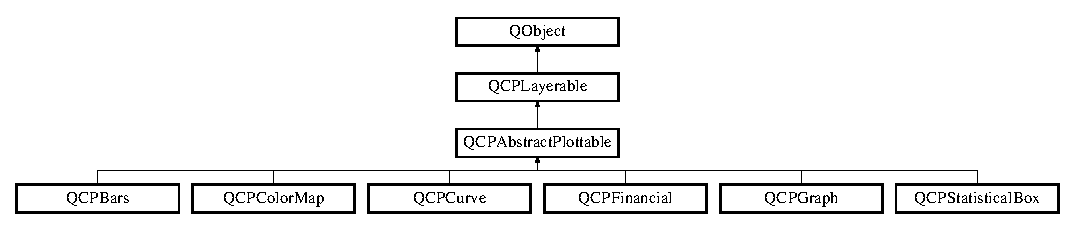
\includegraphics[height=2.629108cm]{class_q_c_p_abstract_plottable}
\end{center}
\end{figure}
\subsection*{Signals}
\begin{DoxyCompactItemize}
\item 
void \hyperlink{class_q_c_p_abstract_plottable_a3af66432b1dca93b28e00e78a8c7c1d9}{selection\+Changed} (bool selected)
\item 
void \hyperlink{class_q_c_p_abstract_plottable_a0059caa3f3581f3959660fef8cbb71c4}{selectable\+Changed} (bool selectable)
\end{DoxyCompactItemize}
\subsection*{Public Member Functions}
\begin{DoxyCompactItemize}
\item 
\hyperlink{class_q_c_p_abstract_plottable_af78a036e40db6f53a31abadc5323715a}{Q\+C\+P\+Abstract\+Plottable} (\hyperlink{class_q_c_p_axis}{Q\+C\+P\+Axis} $\ast$key\+Axis, \hyperlink{class_q_c_p_axis}{Q\+C\+P\+Axis} $\ast$value\+Axis)
\item 
\hypertarget{class_q_c_p_abstract_plottable_a52c226eefcb1920240eeabae574d28c0}{}\label{class_q_c_p_abstract_plottable_a52c226eefcb1920240eeabae574d28c0} 
Q\+String {\bfseries name} () const
\item 
\hypertarget{class_q_c_p_abstract_plottable_a022717896dc57b638a7b5a7be7212ba9}{}\label{class_q_c_p_abstract_plottable_a022717896dc57b638a7b5a7be7212ba9} 
bool {\bfseries antialiased\+Fill} () const
\item 
\hypertarget{class_q_c_p_abstract_plottable_a795370db6b1309de0ab60b633efb5ec2}{}\label{class_q_c_p_abstract_plottable_a795370db6b1309de0ab60b633efb5ec2} 
bool {\bfseries antialiased\+Scatters} () const
\item 
\hypertarget{class_q_c_p_abstract_plottable_add06e122d84deb9f451ace9bb8ad9c96}{}\label{class_q_c_p_abstract_plottable_add06e122d84deb9f451ace9bb8ad9c96} 
bool {\bfseries antialiased\+Error\+Bars} () const
\item 
\hypertarget{class_q_c_p_abstract_plottable_ad5972efc31344e5a7a78ab4f8864b2d3}{}\label{class_q_c_p_abstract_plottable_ad5972efc31344e5a7a78ab4f8864b2d3} 
Q\+Pen {\bfseries pen} () const
\item 
\hypertarget{class_q_c_p_abstract_plottable_aafdfd0946b18364321ffce01cc6045a0}{}\label{class_q_c_p_abstract_plottable_aafdfd0946b18364321ffce01cc6045a0} 
Q\+Pen {\bfseries selected\+Pen} () const
\item 
\hypertarget{class_q_c_p_abstract_plottable_a893b4896dfd92b68b05b2600b80f5826}{}\label{class_q_c_p_abstract_plottable_a893b4896dfd92b68b05b2600b80f5826} 
Q\+Brush {\bfseries brush} () const
\item 
\hypertarget{class_q_c_p_abstract_plottable_afe5f3f74b09e89713ba39da04079a337}{}\label{class_q_c_p_abstract_plottable_afe5f3f74b09e89713ba39da04079a337} 
Q\+Brush {\bfseries selected\+Brush} () const
\item 
\hypertarget{class_q_c_p_abstract_plottable_a2cdd6f0dd5e9a979037f86b4000d9cfe}{}\label{class_q_c_p_abstract_plottable_a2cdd6f0dd5e9a979037f86b4000d9cfe} 
\hyperlink{class_q_c_p_axis}{Q\+C\+P\+Axis} $\ast$ {\bfseries key\+Axis} () const
\item 
\hypertarget{class_q_c_p_abstract_plottable_af47809a644a68ffd955fb30b01fb4f2f}{}\label{class_q_c_p_abstract_plottable_af47809a644a68ffd955fb30b01fb4f2f} 
\hyperlink{class_q_c_p_axis}{Q\+C\+P\+Axis} $\ast$ {\bfseries value\+Axis} () const
\item 
\hypertarget{class_q_c_p_abstract_plottable_adf896b8a213fea74440c7bc969cf6e4c}{}\label{class_q_c_p_abstract_plottable_adf896b8a213fea74440c7bc969cf6e4c} 
bool {\bfseries selectable} () const
\item 
\hypertarget{class_q_c_p_abstract_plottable_a0b3b514474fe93354fc74cfc144184b4}{}\label{class_q_c_p_abstract_plottable_a0b3b514474fe93354fc74cfc144184b4} 
bool {\bfseries selected} () const
\item 
void \hyperlink{class_q_c_p_abstract_plottable_ab79c7ba76bc7fa89a4b3580e12149f1f}{set\+Name} (const Q\+String \&name)
\item 
void \hyperlink{class_q_c_p_abstract_plottable_a089d6b5577120239b55c39ed27c39536}{set\+Antialiased\+Fill} (bool enabled)
\item 
void \hyperlink{class_q_c_p_abstract_plottable_a2f03f067ede2ed4da6f7d0e4777a3f02}{set\+Antialiased\+Scatters} (bool enabled)
\item 
void \hyperlink{class_q_c_p_abstract_plottable_a757beb744b96cf1855cca5ab9d3ecf52}{set\+Antialiased\+Error\+Bars} (bool enabled)
\item 
void \hyperlink{class_q_c_p_abstract_plottable_ab74b09ae4c0e7e13142fe4b5bf46cac7}{set\+Pen} (const Q\+Pen \&pen)
\item 
void \hyperlink{class_q_c_p_abstract_plottable_a6911603cad23ab0469b108224517516f}{set\+Selected\+Pen} (const Q\+Pen \&pen)
\item 
void \hyperlink{class_q_c_p_abstract_plottable_a7a4b92144dca6453a1f0f210e27edc74}{set\+Brush} (const Q\+Brush \&brush)
\item 
void \hyperlink{class_q_c_p_abstract_plottable_ae8c816874089f7a44001e8618e81a9dc}{set\+Selected\+Brush} (const Q\+Brush \&brush)
\item 
void \hyperlink{class_q_c_p_abstract_plottable_a8524fa2994c63c0913ebd9bb2ffa3920}{set\+Key\+Axis} (\hyperlink{class_q_c_p_axis}{Q\+C\+P\+Axis} $\ast$axis)
\item 
void \hyperlink{class_q_c_p_abstract_plottable_a71626a07367e241ec62ad2c34baf21cb}{set\+Value\+Axis} (\hyperlink{class_q_c_p_axis}{Q\+C\+P\+Axis} $\ast$axis)
\item 
Q\+\_\+\+S\+L\+OT void \hyperlink{class_q_c_p_abstract_plottable_a22c69299eb5569e0f6bf084877a37dc4}{set\+Selectable} (bool selectable)
\item 
Q\+\_\+\+S\+L\+OT void \hyperlink{class_q_c_p_abstract_plottable_afbd5428c2952f59d952e11ab5cd79176}{set\+Selected} (bool selected)
\item 
virtual void \hyperlink{class_q_c_p_abstract_plottable_a86e5b8fd4b6ff4f4084e7ea4c573fc53}{clear\+Data} ()=0
\item 
virtual double \hyperlink{class_q_c_p_abstract_plottable_a38efe9641d972992a3d44204bc80ec1d}{select\+Test} (const Q\+PointF \&pos, bool only\+Selectable, Q\+Variant $\ast$details=0) const =0
\item 
virtual bool \hyperlink{class_q_c_p_abstract_plottable_a70f8cabfd808f7d5204b9f18c45c13f5}{add\+To\+Legend} ()
\item 
virtual bool \hyperlink{class_q_c_p_abstract_plottable_ac95fb2604d9106d0852ad9ceb326fe8c}{remove\+From\+Legend} () const
\item 
void \hyperlink{class_q_c_p_abstract_plottable_a1491c4a606bccd2d09e65e11b79eb882}{rescale\+Axes} (bool only\+Enlarge=false) const
\item 
void \hyperlink{class_q_c_p_abstract_plottable_ae96b83c961e257da116c6acf9c7da308}{rescale\+Key\+Axis} (bool only\+Enlarge=false) const
\item 
void \hyperlink{class_q_c_p_abstract_plottable_aa1e408bb2d13999150c3f7f8a8579ca9}{rescale\+Value\+Axis} (bool only\+Enlarge=false) const
\end{DoxyCompactItemize}
\subsection*{Protected Types}
\begin{DoxyCompactItemize}
\item 
enum \hyperlink{class_q_c_p_abstract_plottable_a661743478a1d3c09d28ec2711d7653d8}{Sign\+Domain} \{ \hyperlink{class_q_c_p_abstract_plottable_a661743478a1d3c09d28ec2711d7653d8a0fc9a70796ef60ad18ddd18056e6dc63}{sd\+Negative}, 
\hyperlink{class_q_c_p_abstract_plottable_a661743478a1d3c09d28ec2711d7653d8a082b98cfb91a7363a3b5cd17b0c1cd60}{sd\+Both}, 
\hyperlink{class_q_c_p_abstract_plottable_a661743478a1d3c09d28ec2711d7653d8a02951859f243a4d24e779cfbb5471030}{sd\+Positive}
 \}
\end{DoxyCompactItemize}
\subsection*{Protected Member Functions}
\begin{DoxyCompactItemize}
\item 
\hypertarget{class_q_c_p_abstract_plottable_aafb817dbea97d2798967f3371a701413}{}\label{class_q_c_p_abstract_plottable_aafb817dbea97d2798967f3371a701413} 
virtual Q\+Rect {\bfseries clip\+Rect} () const
\item 
\hypertarget{class_q_c_p_abstract_plottable_acbab5e30dcd04fd302b4a5902ac2c482}{}\label{class_q_c_p_abstract_plottable_acbab5e30dcd04fd302b4a5902ac2c482} 
virtual void {\bfseries draw} (\hyperlink{class_q_c_p_painter}{Q\+C\+P\+Painter} $\ast$painter)=0
\item 
\hypertarget{class_q_c_p_abstract_plottable_afb5e4718c232a16d0fb06b00e172be9e}{}\label{class_q_c_p_abstract_plottable_afb5e4718c232a16d0fb06b00e172be9e} 
virtual \hyperlink{namespace_q_c_p_a2ad6bb6281c7c2d593d4277b44c2b037}{Q\+C\+P\+::\+Interaction} {\bfseries selection\+Category} () const
\item 
\hypertarget{class_q_c_p_abstract_plottable_a59a80773c5cefc05a0646ac8e1149ed5}{}\label{class_q_c_p_abstract_plottable_a59a80773c5cefc05a0646ac8e1149ed5} 
void {\bfseries apply\+Default\+Antialiasing\+Hint} (\hyperlink{class_q_c_p_painter}{Q\+C\+P\+Painter} $\ast$painter) const
\item 
\hypertarget{class_q_c_p_abstract_plottable_a16aaad02456aa23a759efd1ac90c79bf}{}\label{class_q_c_p_abstract_plottable_a16aaad02456aa23a759efd1ac90c79bf} 
virtual void {\bfseries select\+Event} (Q\+Mouse\+Event $\ast$event, bool additive, const Q\+Variant \&details, bool $\ast$selection\+State\+Changed)
\item 
\hypertarget{class_q_c_p_abstract_plottable_a6fa0d0f95560ea8b01ee13f296dab2b1}{}\label{class_q_c_p_abstract_plottable_a6fa0d0f95560ea8b01ee13f296dab2b1} 
virtual void {\bfseries deselect\+Event} (bool $\ast$selection\+State\+Changed)
\item 
\hypertarget{class_q_c_p_abstract_plottable_a9a450783fd9ed539e589999fd390cdf7}{}\label{class_q_c_p_abstract_plottable_a9a450783fd9ed539e589999fd390cdf7} 
virtual void {\bfseries draw\+Legend\+Icon} (\hyperlink{class_q_c_p_painter}{Q\+C\+P\+Painter} $\ast$painter, const Q\+RectF \&rect) const =0
\item 
\hypertarget{class_q_c_p_abstract_plottable_a345d702b2e7e12c8cfdddff65ba85e8c}{}\label{class_q_c_p_abstract_plottable_a345d702b2e7e12c8cfdddff65ba85e8c} 
virtual \hyperlink{class_q_c_p_range}{Q\+C\+P\+Range} {\bfseries get\+Key\+Range} (bool \&found\+Range, \hyperlink{class_q_c_p_abstract_plottable_a661743478a1d3c09d28ec2711d7653d8}{Sign\+Domain} in\+Sign\+Domain=\hyperlink{class_q_c_p_abstract_plottable_a661743478a1d3c09d28ec2711d7653d8a082b98cfb91a7363a3b5cd17b0c1cd60}{sd\+Both}) const =0
\item 
\hypertarget{class_q_c_p_abstract_plottable_aa3331b415b5939fe4df60b78831b2799}{}\label{class_q_c_p_abstract_plottable_aa3331b415b5939fe4df60b78831b2799} 
virtual \hyperlink{class_q_c_p_range}{Q\+C\+P\+Range} {\bfseries get\+Value\+Range} (bool \&found\+Range, \hyperlink{class_q_c_p_abstract_plottable_a661743478a1d3c09d28ec2711d7653d8}{Sign\+Domain} in\+Sign\+Domain=\hyperlink{class_q_c_p_abstract_plottable_a661743478a1d3c09d28ec2711d7653d8a082b98cfb91a7363a3b5cd17b0c1cd60}{sd\+Both}) const =0
\item 
\hypertarget{class_q_c_p_abstract_plottable_a7ad84a36472441cf1f555c5683d0da93}{}\label{class_q_c_p_abstract_plottable_a7ad84a36472441cf1f555c5683d0da93} 
void {\bfseries coords\+To\+Pixels} (double key, double value, double \&x, double \&y) const
\item 
\hypertarget{class_q_c_p_abstract_plottable_a5acb50ae984eef09a7ab92315d2ad708}{}\label{class_q_c_p_abstract_plottable_a5acb50ae984eef09a7ab92315d2ad708} 
const Q\+PointF {\bfseries coords\+To\+Pixels} (double key, double value) const
\item 
\hypertarget{class_q_c_p_abstract_plottable_a3903c1120ab5c27e7fa46b597ef267bd}{}\label{class_q_c_p_abstract_plottable_a3903c1120ab5c27e7fa46b597ef267bd} 
void {\bfseries pixels\+To\+Coords} (double x, double y, double \&key, double \&value) const
\item 
\hypertarget{class_q_c_p_abstract_plottable_a28d32c0062b9450847851ffdee1c5f69}{}\label{class_q_c_p_abstract_plottable_a28d32c0062b9450847851ffdee1c5f69} 
void {\bfseries pixels\+To\+Coords} (const Q\+PointF \&pixel\+Pos, double \&key, double \&value) const
\item 
\hypertarget{class_q_c_p_abstract_plottable_abd790a3b229239f49067f136633a4b98}{}\label{class_q_c_p_abstract_plottable_abd790a3b229239f49067f136633a4b98} 
Q\+Pen {\bfseries main\+Pen} () const
\item 
\hypertarget{class_q_c_p_abstract_plottable_ac9147022a662e92b46c39e7cb821b0af}{}\label{class_q_c_p_abstract_plottable_ac9147022a662e92b46c39e7cb821b0af} 
Q\+Brush {\bfseries main\+Brush} () const
\item 
\hypertarget{class_q_c_p_abstract_plottable_a8d06a59ea23324cce6330ebf2262c0ed}{}\label{class_q_c_p_abstract_plottable_a8d06a59ea23324cce6330ebf2262c0ed} 
void {\bfseries apply\+Fill\+Antialiasing\+Hint} (\hyperlink{class_q_c_p_painter}{Q\+C\+P\+Painter} $\ast$painter) const
\item 
\hypertarget{class_q_c_p_abstract_plottable_ac95f26b15a1e5d9c7bd2c0a46d760fc9}{}\label{class_q_c_p_abstract_plottable_ac95f26b15a1e5d9c7bd2c0a46d760fc9} 
void {\bfseries apply\+Scatters\+Antialiasing\+Hint} (\hyperlink{class_q_c_p_painter}{Q\+C\+P\+Painter} $\ast$painter) const
\item 
\hypertarget{class_q_c_p_abstract_plottable_a0889abc8dbfd357053f40bfafff8bf7d}{}\label{class_q_c_p_abstract_plottable_a0889abc8dbfd357053f40bfafff8bf7d} 
void {\bfseries apply\+Error\+Bars\+Antialiasing\+Hint} (\hyperlink{class_q_c_p_painter}{Q\+C\+P\+Painter} $\ast$painter) const
\item 
\hypertarget{class_q_c_p_abstract_plottable_af7e992b638c8aa688abceac579bb90d7}{}\label{class_q_c_p_abstract_plottable_af7e992b638c8aa688abceac579bb90d7} 
double {\bfseries dist\+Sqr\+To\+Line} (const Q\+PointF \&start, const Q\+PointF \&end, const Q\+PointF \&point) const
\end{DoxyCompactItemize}
\subsection*{Protected Attributes}
\begin{DoxyCompactItemize}
\item 
\hypertarget{class_q_c_p_abstract_plottable_ac29ffef424e2488675930de18cde612a}{}\label{class_q_c_p_abstract_plottable_ac29ffef424e2488675930de18cde612a} 
Q\+String {\bfseries m\+Name}
\item 
\hypertarget{class_q_c_p_abstract_plottable_a152ac765bedf927fb240545d11d453ea}{}\label{class_q_c_p_abstract_plottable_a152ac765bedf927fb240545d11d453ea} 
bool {\bfseries m\+Antialiased\+Fill}
\item 
\hypertarget{class_q_c_p_abstract_plottable_aa115755e525a8e3a86dc683f9cab755b}{}\label{class_q_c_p_abstract_plottable_aa115755e525a8e3a86dc683f9cab755b} 
bool {\bfseries m\+Antialiased\+Scatters}
\item 
\hypertarget{class_q_c_p_abstract_plottable_ad48660b2bd301576e92fb033d8f455ea}{}\label{class_q_c_p_abstract_plottable_ad48660b2bd301576e92fb033d8f455ea} 
bool {\bfseries m\+Antialiased\+Error\+Bars}
\item 
\hypertarget{class_q_c_p_abstract_plottable_a67bc0622fd1b9fa14e54c14922dcec66}{}\label{class_q_c_p_abstract_plottable_a67bc0622fd1b9fa14e54c14922dcec66} 
Q\+Pen {\bfseries m\+Pen}
\item 
\hypertarget{class_q_c_p_abstract_plottable_a10619472f5d5e10e9519a599f1cf5576}{}\label{class_q_c_p_abstract_plottable_a10619472f5d5e10e9519a599f1cf5576} 
Q\+Pen {\bfseries m\+Selected\+Pen}
\item 
\hypertarget{class_q_c_p_abstract_plottable_a33f00674c0161c13315ab9da0895418e}{}\label{class_q_c_p_abstract_plottable_a33f00674c0161c13315ab9da0895418e} 
Q\+Brush {\bfseries m\+Brush}
\item 
\hypertarget{class_q_c_p_abstract_plottable_aea3c0da30c7a8be23ad5f2d9bca36762}{}\label{class_q_c_p_abstract_plottable_aea3c0da30c7a8be23ad5f2d9bca36762} 
Q\+Brush {\bfseries m\+Selected\+Brush}
\item 
\hypertarget{class_q_c_p_abstract_plottable_a426f42e254d0f8ce5436a868c61a6827}{}\label{class_q_c_p_abstract_plottable_a426f42e254d0f8ce5436a868c61a6827} 
Q\+Pointer$<$ \hyperlink{class_q_c_p_axis}{Q\+C\+P\+Axis} $>$ {\bfseries m\+Key\+Axis}
\item 
\hypertarget{class_q_c_p_abstract_plottable_a2901452ca4aea911a1827717934a4bda}{}\label{class_q_c_p_abstract_plottable_a2901452ca4aea911a1827717934a4bda} 
Q\+Pointer$<$ \hyperlink{class_q_c_p_axis}{Q\+C\+P\+Axis} $>$ {\bfseries m\+Value\+Axis}
\item 
\hypertarget{class_q_c_p_abstract_plottable_aceee52342c8e75727abcbd164986fdcb}{}\label{class_q_c_p_abstract_plottable_aceee52342c8e75727abcbd164986fdcb} 
bool {\bfseries m\+Selectable}
\item 
\hypertarget{class_q_c_p_abstract_plottable_a43f68a0603e9bcd016bdfa6d9d5c41c9}{}\label{class_q_c_p_abstract_plottable_a43f68a0603e9bcd016bdfa6d9d5c41c9} 
bool {\bfseries m\+Selected}
\end{DoxyCompactItemize}
\subsection*{Friends}
\begin{DoxyCompactItemize}
\item 
\hypertarget{class_q_c_p_abstract_plottable_a1cdf9df76adcfae45261690aa0ca2198}{}\label{class_q_c_p_abstract_plottable_a1cdf9df76adcfae45261690aa0ca2198} 
class {\bfseries Q\+Custom\+Plot}
\item 
\hypertarget{class_q_c_p_abstract_plottable_af123edeca169ec7a31958a1d714e1a8a}{}\label{class_q_c_p_abstract_plottable_af123edeca169ec7a31958a1d714e1a8a} 
class {\bfseries Q\+C\+P\+Axis}
\item 
\hypertarget{class_q_c_p_abstract_plottable_a104c78e91302afd6842a903e472f552f}{}\label{class_q_c_p_abstract_plottable_a104c78e91302afd6842a903e472f552f} 
class {\bfseries Q\+C\+P\+Plottable\+Legend\+Item}
\end{DoxyCompactItemize}


\subsection{Detailed Description}
The abstract base class for all data representing objects in a plot. 

It defines a very basic interface like name, pen, brush, visibility etc. Since this class is abstract, it can\textquotesingle{}t be instantiated. Use one of the subclasses or create a subclass yourself to create new ways of displaying data (see \char`\"{}\+Creating own plottables\char`\"{} below).

All further specifics are in the subclasses, for example\+: \begin{DoxyItemize}
\item A normal graph with possibly a line, scatter points and error bars\+: \hyperlink{class_q_c_p_graph}{Q\+C\+P\+Graph} (typically created with \hyperlink{class_q_custom_plot_a6fb2873d35a8a8089842d81a70a54167}{Q\+Custom\+Plot\+::add\+Graph}) \item A parametric curve\+: \hyperlink{class_q_c_p_curve}{Q\+C\+P\+Curve} \item A bar chart\+: \hyperlink{class_q_c_p_bars}{Q\+C\+P\+Bars} \item A statistical box plot\+: \hyperlink{class_q_c_p_statistical_box}{Q\+C\+P\+Statistical\+Box} \item A color encoded two-\/dimensional map\+: \hyperlink{class_q_c_p_color_map}{Q\+C\+P\+Color\+Map} \item An O\+H\+L\+C/\+Candlestick chart\+: \hyperlink{class_q_c_p_financial}{Q\+C\+P\+Financial}\end{DoxyItemize}
\hypertarget{class_q_c_p_abstract_plottable_plottables-subclassing}{}\subsection{Creating own plottables}\label{class_q_c_p_abstract_plottable_plottables-subclassing}
To create an own plottable, you implement a subclass of \hyperlink{class_q_c_p_abstract_plottable}{Q\+C\+P\+Abstract\+Plottable}. These are the pure virtual functions, you must implement\+: \begin{DoxyItemize}
\item \hyperlink{class_q_c_p_abstract_plottable_a86e5b8fd4b6ff4f4084e7ea4c573fc53}{clear\+Data} \item \hyperlink{class_q_c_p_abstract_plottable_a38efe9641d972992a3d44204bc80ec1d}{select\+Test} \item draw \item draw\+Legend\+Icon \item get\+Key\+Range \item get\+Value\+Range\end{DoxyItemize}
See the documentation of those functions for what they need to do.

For drawing your plot, you can use the coords\+To\+Pixels functions to translate a point in plot coordinates to pixel coordinates. This function is quite convenient, because it takes the orientation of the key and value axes into account for you (x and y are swapped when the key axis is vertical and the value axis horizontal). If you are worried about performance (i.\+e. you need to translate many points in a loop like \hyperlink{class_q_c_p_graph}{Q\+C\+P\+Graph}), you can directly use \hyperlink{class_q_c_p_axis_af15d1b3a7f7e9b53d759d3ccff1fe4b4}{Q\+C\+P\+Axis\+::coord\+To\+Pixel}. However, you must then take care about the orientation of the axis yourself.

Here are some important members you inherit from \hyperlink{class_q_c_p_abstract_plottable}{Q\+C\+P\+Abstract\+Plottable}\+: \tabulinesep=1mm
\begin{longtabu} spread 0pt [c]{*{2}{|X[-1]}|}
\hline
\hyperlink{class_q_custom_plot}{Q\+Custom\+Plot} $\ast${\bfseries m\+Parent\+Plot}  &A pointer to the parent \hyperlink{class_q_custom_plot}{Q\+Custom\+Plot} instance. The parent plot is inferred from the axes that are passed in the constructor. \\\cline{1-2}
Q\+String {\bfseries m\+Name}  &The name of the plottable. \\\cline{1-2}
Q\+Pen {\bfseries m\+Pen}  &The generic pen of the plottable. You should use this pen for the most prominent data representing lines in the plottable (e.\+g \hyperlink{class_q_c_p_graph}{Q\+C\+P\+Graph} uses this pen for its graph lines and scatters) \\\cline{1-2}
Q\+Pen {\bfseries m\+Selected\+Pen}  &The generic pen that should be used when the plottable is selected (hint\+: main\+Pen gives you the right pen, depending on selection state). \\\cline{1-2}
Q\+Brush {\bfseries m\+Brush}  &The generic brush of the plottable. You should use this brush for the most prominent fillable structures in the plottable (e.\+g. \hyperlink{class_q_c_p_graph}{Q\+C\+P\+Graph} uses this brush to control filling under the graph) \\\cline{1-2}
Q\+Brush {\bfseries m\+Selected\+Brush}  &The generic brush that should be used when the plottable is selected (hint\+: main\+Brush gives you the right brush, depending on selection state). \\\cline{1-2}
Q\+Pointer$<$\+Q\+C\+P\+Axis$>${\bfseries m\+Key\+Axis}, {\bfseries m\+Value\+Axis}  &The key and value axes this plottable is attached to. Call their \hyperlink{class_q_c_p_axis_af15d1b3a7f7e9b53d759d3ccff1fe4b4}{Q\+C\+P\+Axis\+::coord\+To\+Pixel} functions to translate coordinates to pixels in either the key or value dimension. Make sure to check whether the pointer is null before using it. If one of the axes is null, don\textquotesingle{}t draw the plottable. \\\cline{1-2}
bool {\bfseries m\+Selected}  &indicates whether the plottable is selected or not.  \\\cline{1-2}
\end{longtabu}


\subsection{Member Enumeration Documentation}
\hypertarget{class_q_c_p_abstract_plottable_a661743478a1d3c09d28ec2711d7653d8}{}\label{class_q_c_p_abstract_plottable_a661743478a1d3c09d28ec2711d7653d8} 
\index{Q\+C\+P\+Abstract\+Plottable@{Q\+C\+P\+Abstract\+Plottable}!Sign\+Domain@{Sign\+Domain}}
\index{Sign\+Domain@{Sign\+Domain}!Q\+C\+P\+Abstract\+Plottable@{Q\+C\+P\+Abstract\+Plottable}}
\subsubsection{\texorpdfstring{Sign\+Domain}{SignDomain}}
{\footnotesize\ttfamily enum \hyperlink{class_q_c_p_abstract_plottable_a661743478a1d3c09d28ec2711d7653d8}{Q\+C\+P\+Abstract\+Plottable\+::\+Sign\+Domain}\hspace{0.3cm}{\ttfamily [protected]}}

Represents negative and positive sign domain for passing to get\+Key\+Range and get\+Value\+Range. \begin{DoxyEnumFields}{Enumerator}
\raisebox{\heightof{T}}[0pt][0pt]{\index{sd\+Negative@{sd\+Negative}!Q\+C\+P\+Abstract\+Plottable@{Q\+C\+P\+Abstract\+Plottable}}\index{Q\+C\+P\+Abstract\+Plottable@{Q\+C\+P\+Abstract\+Plottable}!sd\+Negative@{sd\+Negative}}}\hypertarget{class_q_c_p_abstract_plottable_a661743478a1d3c09d28ec2711d7653d8a0fc9a70796ef60ad18ddd18056e6dc63}{}\label{class_q_c_p_abstract_plottable_a661743478a1d3c09d28ec2711d7653d8a0fc9a70796ef60ad18ddd18056e6dc63} 
sd\+Negative&The negative sign domain, i.\+e. numbers smaller than zero. \\
\hline

\raisebox{\heightof{T}}[0pt][0pt]{\index{sd\+Both@{sd\+Both}!Q\+C\+P\+Abstract\+Plottable@{Q\+C\+P\+Abstract\+Plottable}}\index{Q\+C\+P\+Abstract\+Plottable@{Q\+C\+P\+Abstract\+Plottable}!sd\+Both@{sd\+Both}}}\hypertarget{class_q_c_p_abstract_plottable_a661743478a1d3c09d28ec2711d7653d8a082b98cfb91a7363a3b5cd17b0c1cd60}{}\label{class_q_c_p_abstract_plottable_a661743478a1d3c09d28ec2711d7653d8a082b98cfb91a7363a3b5cd17b0c1cd60} 
sd\+Both&Both sign domains, including zero, i.\+e. all (rational) numbers. \\
\hline

\raisebox{\heightof{T}}[0pt][0pt]{\index{sd\+Positive@{sd\+Positive}!Q\+C\+P\+Abstract\+Plottable@{Q\+C\+P\+Abstract\+Plottable}}\index{Q\+C\+P\+Abstract\+Plottable@{Q\+C\+P\+Abstract\+Plottable}!sd\+Positive@{sd\+Positive}}}\hypertarget{class_q_c_p_abstract_plottable_a661743478a1d3c09d28ec2711d7653d8a02951859f243a4d24e779cfbb5471030}{}\label{class_q_c_p_abstract_plottable_a661743478a1d3c09d28ec2711d7653d8a02951859f243a4d24e779cfbb5471030} 
sd\+Positive&The positive sign domain, i.\+e. numbers greater than zero. \\
\hline

\end{DoxyEnumFields}


\subsection{Constructor \& Destructor Documentation}
\hypertarget{class_q_c_p_abstract_plottable_af78a036e40db6f53a31abadc5323715a}{}\label{class_q_c_p_abstract_plottable_af78a036e40db6f53a31abadc5323715a} 
\index{Q\+C\+P\+Abstract\+Plottable@{Q\+C\+P\+Abstract\+Plottable}!Q\+C\+P\+Abstract\+Plottable@{Q\+C\+P\+Abstract\+Plottable}}
\index{Q\+C\+P\+Abstract\+Plottable@{Q\+C\+P\+Abstract\+Plottable}!Q\+C\+P\+Abstract\+Plottable@{Q\+C\+P\+Abstract\+Plottable}}
\subsubsection{\texorpdfstring{Q\+C\+P\+Abstract\+Plottable()}{QCPAbstractPlottable()}}
{\footnotesize\ttfamily Q\+C\+P\+Abstract\+Plottable\+::\+Q\+C\+P\+Abstract\+Plottable (\begin{DoxyParamCaption}\item[{\hyperlink{class_q_c_p_axis}{Q\+C\+P\+Axis} $\ast$}]{key\+Axis,  }\item[{\hyperlink{class_q_c_p_axis}{Q\+C\+P\+Axis} $\ast$}]{value\+Axis }\end{DoxyParamCaption})}

Constructs an abstract plottable which uses {\itshape key\+Axis} as its key axis (\char`\"{}x\char`\"{}) and {\itshape value\+Axis} as its value axis (\char`\"{}y\char`\"{}). {\itshape key\+Axis} and {\itshape value\+Axis} must reside in the same \hyperlink{class_q_custom_plot}{Q\+Custom\+Plot} instance and have perpendicular orientations. If either of these restrictions is violated, a corresponding message is printed to the debug output (q\+Debug), the construction is not aborted, though.

Since \hyperlink{class_q_c_p_abstract_plottable}{Q\+C\+P\+Abstract\+Plottable} is an abstract class that defines the basic interface to plottables, it can\textquotesingle{}t be directly instantiated.

You probably want one of the subclasses like \hyperlink{class_q_c_p_graph}{Q\+C\+P\+Graph} or \hyperlink{class_q_c_p_curve}{Q\+C\+P\+Curve} instead. 

\subsection{Member Function Documentation}
\hypertarget{class_q_c_p_abstract_plottable_a70f8cabfd808f7d5204b9f18c45c13f5}{}\label{class_q_c_p_abstract_plottable_a70f8cabfd808f7d5204b9f18c45c13f5} 
\index{Q\+C\+P\+Abstract\+Plottable@{Q\+C\+P\+Abstract\+Plottable}!add\+To\+Legend@{add\+To\+Legend}}
\index{add\+To\+Legend@{add\+To\+Legend}!Q\+C\+P\+Abstract\+Plottable@{Q\+C\+P\+Abstract\+Plottable}}
\subsubsection{\texorpdfstring{add\+To\+Legend()}{addToLegend()}}
{\footnotesize\ttfamily bool Q\+C\+P\+Abstract\+Plottable\+::add\+To\+Legend (\begin{DoxyParamCaption}{ }\end{DoxyParamCaption})\hspace{0.3cm}{\ttfamily [virtual]}}

Adds this plottable to the legend of the parent \hyperlink{class_q_custom_plot}{Q\+Custom\+Plot} (\hyperlink{class_q_custom_plot_a4eadcd237dc6a09938b68b16877fa6af}{Q\+Custom\+Plot\+::legend}).

Normally, a \hyperlink{class_q_c_p_plottable_legend_item}{Q\+C\+P\+Plottable\+Legend\+Item} is created and inserted into the legend. If the plottable needs a more specialized representation in the legend, this function will take this into account and instead create the specialized subclass of \hyperlink{class_q_c_p_abstract_legend_item}{Q\+C\+P\+Abstract\+Legend\+Item}.

Returns true on success, i.\+e. when the legend exists and a legend item associated with this plottable isn\textquotesingle{}t already in the legend.

\begin{DoxySeeAlso}{See also}
\hyperlink{class_q_c_p_abstract_plottable_ac95fb2604d9106d0852ad9ceb326fe8c}{remove\+From\+Legend}, \hyperlink{class_q_c_p_legend_a3ab274de52d2951faea45a6d975e6b3f}{Q\+C\+P\+Legend\+::add\+Item} 
\end{DoxySeeAlso}
\hypertarget{class_q_c_p_abstract_plottable_a86e5b8fd4b6ff4f4084e7ea4c573fc53}{}\label{class_q_c_p_abstract_plottable_a86e5b8fd4b6ff4f4084e7ea4c573fc53} 
\index{Q\+C\+P\+Abstract\+Plottable@{Q\+C\+P\+Abstract\+Plottable}!clear\+Data@{clear\+Data}}
\index{clear\+Data@{clear\+Data}!Q\+C\+P\+Abstract\+Plottable@{Q\+C\+P\+Abstract\+Plottable}}
\subsubsection{\texorpdfstring{clear\+Data()}{clearData()}}
{\footnotesize\ttfamily void Q\+C\+P\+Abstract\+Plottable\+::clear\+Data (\begin{DoxyParamCaption}{ }\end{DoxyParamCaption})\hspace{0.3cm}{\ttfamily [pure virtual]}}

Clears all data in the plottable. 

Implemented in \hyperlink{class_q_c_p_financial_a11fd49928c33e55e27b7319c6927864a}{Q\+C\+P\+Financial}, \hyperlink{class_q_c_p_color_map_a0545dce5383766885912331705a8e099}{Q\+C\+P\+Color\+Map}, \hyperlink{class_q_c_p_statistical_box_a19112994449df0c20287858436cc68e3}{Q\+C\+P\+Statistical\+Box}, \hyperlink{class_q_c_p_bars_a11dbbd707132f07f862dff13c5789c2b}{Q\+C\+P\+Bars}, \hyperlink{class_q_c_p_curve_ae0462c61dbfbac07db0736ec64110241}{Q\+C\+P\+Curve}, and \hyperlink{class_q_c_p_graph_ad4e94a4e44e5e76fbec81a72a977157d}{Q\+C\+P\+Graph}.

\hypertarget{class_q_c_p_abstract_plottable_ac95fb2604d9106d0852ad9ceb326fe8c}{}\label{class_q_c_p_abstract_plottable_ac95fb2604d9106d0852ad9ceb326fe8c} 
\index{Q\+C\+P\+Abstract\+Plottable@{Q\+C\+P\+Abstract\+Plottable}!remove\+From\+Legend@{remove\+From\+Legend}}
\index{remove\+From\+Legend@{remove\+From\+Legend}!Q\+C\+P\+Abstract\+Plottable@{Q\+C\+P\+Abstract\+Plottable}}
\subsubsection{\texorpdfstring{remove\+From\+Legend()}{removeFromLegend()}}
{\footnotesize\ttfamily bool Q\+C\+P\+Abstract\+Plottable\+::remove\+From\+Legend (\begin{DoxyParamCaption}{ }\end{DoxyParamCaption}) const\hspace{0.3cm}{\ttfamily [virtual]}}

Removes the plottable from the legend of the parent \hyperlink{class_q_custom_plot}{Q\+Custom\+Plot}. This means the \hyperlink{class_q_c_p_abstract_legend_item}{Q\+C\+P\+Abstract\+Legend\+Item} (usually a \hyperlink{class_q_c_p_plottable_legend_item}{Q\+C\+P\+Plottable\+Legend\+Item}) that is associated with this plottable is removed.

Returns true on success, i.\+e. if the legend exists and a legend item associated with this plottable was found and removed.

\begin{DoxySeeAlso}{See also}
\hyperlink{class_q_c_p_abstract_plottable_a70f8cabfd808f7d5204b9f18c45c13f5}{add\+To\+Legend}, \hyperlink{class_q_c_p_legend_ac91595c3eaa746fe6321d2eb952c63bb}{Q\+C\+P\+Legend\+::remove\+Item} 
\end{DoxySeeAlso}
\hypertarget{class_q_c_p_abstract_plottable_a1491c4a606bccd2d09e65e11b79eb882}{}\label{class_q_c_p_abstract_plottable_a1491c4a606bccd2d09e65e11b79eb882} 
\index{Q\+C\+P\+Abstract\+Plottable@{Q\+C\+P\+Abstract\+Plottable}!rescale\+Axes@{rescale\+Axes}}
\index{rescale\+Axes@{rescale\+Axes}!Q\+C\+P\+Abstract\+Plottable@{Q\+C\+P\+Abstract\+Plottable}}
\subsubsection{\texorpdfstring{rescale\+Axes()}{rescaleAxes()}}
{\footnotesize\ttfamily void Q\+C\+P\+Abstract\+Plottable\+::rescale\+Axes (\begin{DoxyParamCaption}\item[{bool}]{only\+Enlarge = {\ttfamily false} }\end{DoxyParamCaption}) const}

Rescales the key and value axes associated with this plottable to contain all displayed data, so the whole plottable is visible. If the scaling of an axis is logarithmic, rescale\+Axes will make sure not to rescale to an illegal range i.\+e. a range containing different signs and/or zero. Instead it will stay in the current sign domain and ignore all parts of the plottable that lie outside of that domain.

{\itshape only\+Enlarge} makes sure the ranges are only expanded, never reduced. So it\textquotesingle{}s possible to show multiple plottables in their entirety by multiple calls to rescale\+Axes where the first call has {\itshape only\+Enlarge} set to false (the default), and all subsequent set to true.

\begin{DoxySeeAlso}{See also}
\hyperlink{class_q_c_p_abstract_plottable_ae96b83c961e257da116c6acf9c7da308}{rescale\+Key\+Axis}, \hyperlink{class_q_c_p_abstract_plottable_aa1e408bb2d13999150c3f7f8a8579ca9}{rescale\+Value\+Axis}, \hyperlink{class_q_custom_plot_ad86528f2cee6c7e446dea4a6e8839935}{Q\+Custom\+Plot\+::rescale\+Axes}, \hyperlink{class_q_c_p_axis_a499345f02ebce4b23d8ccec96e58daa9}{Q\+C\+P\+Axis\+::rescale} 
\end{DoxySeeAlso}
\hypertarget{class_q_c_p_abstract_plottable_ae96b83c961e257da116c6acf9c7da308}{}\label{class_q_c_p_abstract_plottable_ae96b83c961e257da116c6acf9c7da308} 
\index{Q\+C\+P\+Abstract\+Plottable@{Q\+C\+P\+Abstract\+Plottable}!rescale\+Key\+Axis@{rescale\+Key\+Axis}}
\index{rescale\+Key\+Axis@{rescale\+Key\+Axis}!Q\+C\+P\+Abstract\+Plottable@{Q\+C\+P\+Abstract\+Plottable}}
\subsubsection{\texorpdfstring{rescale\+Key\+Axis()}{rescaleKeyAxis()}}
{\footnotesize\ttfamily void Q\+C\+P\+Abstract\+Plottable\+::rescale\+Key\+Axis (\begin{DoxyParamCaption}\item[{bool}]{only\+Enlarge = {\ttfamily false} }\end{DoxyParamCaption}) const}

Rescales the key axis of the plottable so the whole plottable is visible.

See \hyperlink{class_q_c_p_abstract_plottable_a1491c4a606bccd2d09e65e11b79eb882}{rescale\+Axes} for detailed behaviour. \hypertarget{class_q_c_p_abstract_plottable_aa1e408bb2d13999150c3f7f8a8579ca9}{}\label{class_q_c_p_abstract_plottable_aa1e408bb2d13999150c3f7f8a8579ca9} 
\index{Q\+C\+P\+Abstract\+Plottable@{Q\+C\+P\+Abstract\+Plottable}!rescale\+Value\+Axis@{rescale\+Value\+Axis}}
\index{rescale\+Value\+Axis@{rescale\+Value\+Axis}!Q\+C\+P\+Abstract\+Plottable@{Q\+C\+P\+Abstract\+Plottable}}
\subsubsection{\texorpdfstring{rescale\+Value\+Axis()}{rescaleValueAxis()}}
{\footnotesize\ttfamily void Q\+C\+P\+Abstract\+Plottable\+::rescale\+Value\+Axis (\begin{DoxyParamCaption}\item[{bool}]{only\+Enlarge = {\ttfamily false} }\end{DoxyParamCaption}) const}

Rescales the value axis of the plottable so the whole plottable is visible.

Returns true if the axis was actually scaled. This might not be the case if this plottable has an invalid range, e.\+g. because it has no data points.

See \hyperlink{class_q_c_p_abstract_plottable_a1491c4a606bccd2d09e65e11b79eb882}{rescale\+Axes} for detailed behaviour. \hypertarget{class_q_c_p_abstract_plottable_a0059caa3f3581f3959660fef8cbb71c4}{}\label{class_q_c_p_abstract_plottable_a0059caa3f3581f3959660fef8cbb71c4} 
\index{Q\+C\+P\+Abstract\+Plottable@{Q\+C\+P\+Abstract\+Plottable}!selectable\+Changed@{selectable\+Changed}}
\index{selectable\+Changed@{selectable\+Changed}!Q\+C\+P\+Abstract\+Plottable@{Q\+C\+P\+Abstract\+Plottable}}
\subsubsection{\texorpdfstring{selectable\+Changed}{selectableChanged}}
{\footnotesize\ttfamily void Q\+C\+P\+Abstract\+Plottable\+::selectable\+Changed (\begin{DoxyParamCaption}\item[{bool}]{selectable }\end{DoxyParamCaption})\hspace{0.3cm}{\ttfamily [signal]}}

This signal is emitted when the selectability of this plottable has changed.

\begin{DoxySeeAlso}{See also}
\hyperlink{class_q_c_p_abstract_plottable_a22c69299eb5569e0f6bf084877a37dc4}{set\+Selectable} 
\end{DoxySeeAlso}
\hypertarget{class_q_c_p_abstract_plottable_a3af66432b1dca93b28e00e78a8c7c1d9}{}\label{class_q_c_p_abstract_plottable_a3af66432b1dca93b28e00e78a8c7c1d9} 
\index{Q\+C\+P\+Abstract\+Plottable@{Q\+C\+P\+Abstract\+Plottable}!selection\+Changed@{selection\+Changed}}
\index{selection\+Changed@{selection\+Changed}!Q\+C\+P\+Abstract\+Plottable@{Q\+C\+P\+Abstract\+Plottable}}
\subsubsection{\texorpdfstring{selection\+Changed}{selectionChanged}}
{\footnotesize\ttfamily void Q\+C\+P\+Abstract\+Plottable\+::selection\+Changed (\begin{DoxyParamCaption}\item[{bool}]{selected }\end{DoxyParamCaption})\hspace{0.3cm}{\ttfamily [signal]}}

This signal is emitted when the selection state of this plottable has changed, either by user interaction or by a direct call to \hyperlink{class_q_c_p_abstract_plottable_afbd5428c2952f59d952e11ab5cd79176}{set\+Selected}. \hypertarget{class_q_c_p_abstract_plottable_a38efe9641d972992a3d44204bc80ec1d}{}\label{class_q_c_p_abstract_plottable_a38efe9641d972992a3d44204bc80ec1d} 
\index{Q\+C\+P\+Abstract\+Plottable@{Q\+C\+P\+Abstract\+Plottable}!select\+Test@{select\+Test}}
\index{select\+Test@{select\+Test}!Q\+C\+P\+Abstract\+Plottable@{Q\+C\+P\+Abstract\+Plottable}}
\subsubsection{\texorpdfstring{select\+Test()}{selectTest()}}
{\footnotesize\ttfamily virtual double Q\+C\+P\+Abstract\+Plottable\+::select\+Test (\begin{DoxyParamCaption}\item[{const Q\+PointF \&}]{pos,  }\item[{bool}]{only\+Selectable,  }\item[{Q\+Variant $\ast$}]{details = {\ttfamily 0} }\end{DoxyParamCaption}) const\hspace{0.3cm}{\ttfamily [pure virtual]}}

This function is used to decide whether a click hits a layerable object or not.

{\itshape pos} is a point in pixel coordinates on the \hyperlink{class_q_custom_plot}{Q\+Custom\+Plot} surface. This function returns the shortest pixel distance of this point to the object. If the object is either invisible or the distance couldn\textquotesingle{}t be determined, -\/1.\+0 is returned. Further, if {\itshape only\+Selectable} is true and the object is not selectable, -\/1.\+0 is returned, too.

If the object is represented not by single lines but by an area like a \hyperlink{class_q_c_p_item_text}{Q\+C\+P\+Item\+Text} or the bars of a \hyperlink{class_q_c_p_bars}{Q\+C\+P\+Bars} plottable, a click inside the area should also be considered a hit. In these cases this function thus returns a constant value greater zero but still below the parent plot\textquotesingle{}s selection tolerance. (typically the selection\+Tolerance multiplied by 0.\+99).

Providing a constant value for area objects allows selecting line objects even when they are obscured by such area objects, by clicking close to the lines (i.\+e. closer than 0.\+99$\ast$selection\+Tolerance).

The actual setting of the selection state is not done by this function. This is handled by the parent \hyperlink{class_q_custom_plot}{Q\+Custom\+Plot} when the mouse\+Release\+Event occurs, and the finally selected object is notified via the select\+Event/deselect\+Event methods.

{\itshape details} is an optional output parameter. Every layerable subclass may place any information in {\itshape details}. This information will be passed to select\+Event when the parent \hyperlink{class_q_custom_plot}{Q\+Custom\+Plot} decides on the basis of this select\+Test call, that the object was successfully selected. The subsequent call to select\+Event will carry the {\itshape details}. This is useful for multi-\/part objects (like \hyperlink{class_q_c_p_axis}{Q\+C\+P\+Axis}). This way, a possibly complex calculation to decide which part was clicked is only done once in \hyperlink{class_q_c_p_abstract_plottable_a38efe9641d972992a3d44204bc80ec1d}{select\+Test}. The result (i.\+e. the actually clicked part) can then be placed in {\itshape details}. So in the subsequent select\+Event, the decision which part was selected doesn\textquotesingle{}t have to be done a second time for a single selection operation.

You may pass 0 as {\itshape details} to indicate that you are not interested in those selection details.

\begin{DoxySeeAlso}{See also}
select\+Event, deselect\+Event, \hyperlink{class_q_custom_plot_a5ee1e2f6ae27419deca53e75907c27e5}{Q\+Custom\+Plot\+::set\+Interactions} 
\end{DoxySeeAlso}


Reimplemented from \hyperlink{class_q_c_p_layerable_a04db8351fefd44cfdb77958e75c6288e}{Q\+C\+P\+Layerable}.



Implemented in \hyperlink{class_q_c_p_financial_a77bffad8f3fcbcccbef03ead1c538e3a}{Q\+C\+P\+Financial}, \hyperlink{class_q_c_p_color_map_aba91ea58b489031157ecb777fe79e309}{Q\+C\+P\+Color\+Map}, \hyperlink{class_q_c_p_statistical_box_a0153ac16326b94450afbca208e3f9961}{Q\+C\+P\+Statistical\+Box}, \hyperlink{class_q_c_p_bars_a62d66cc8eedca6bedfc1f6513164d418}{Q\+C\+P\+Bars}, \hyperlink{class_q_c_p_curve_a87a9fb34a2a48dcae4c1245ada235e7d}{Q\+C\+P\+Curve}, and \hyperlink{class_q_c_p_graph_a36011c34aca4f7a477de25961e2f6c13}{Q\+C\+P\+Graph}.

\hypertarget{class_q_c_p_abstract_plottable_a757beb744b96cf1855cca5ab9d3ecf52}{}\label{class_q_c_p_abstract_plottable_a757beb744b96cf1855cca5ab9d3ecf52} 
\index{Q\+C\+P\+Abstract\+Plottable@{Q\+C\+P\+Abstract\+Plottable}!set\+Antialiased\+Error\+Bars@{set\+Antialiased\+Error\+Bars}}
\index{set\+Antialiased\+Error\+Bars@{set\+Antialiased\+Error\+Bars}!Q\+C\+P\+Abstract\+Plottable@{Q\+C\+P\+Abstract\+Plottable}}
\subsubsection{\texorpdfstring{set\+Antialiased\+Error\+Bars()}{setAntialiasedErrorBars()}}
{\footnotesize\ttfamily void Q\+C\+P\+Abstract\+Plottable\+::set\+Antialiased\+Error\+Bars (\begin{DoxyParamCaption}\item[{bool}]{enabled }\end{DoxyParamCaption})}

Sets whether the error bars of this plottable are drawn antialiased or not.

Note that this setting may be overridden by \hyperlink{class_q_custom_plot_af6f91e5eab1be85f67c556e98c3745e8}{Q\+Custom\+Plot\+::set\+Antialiased\+Elements} and \hyperlink{class_q_custom_plot_ae10d685b5eabea2999fb8775ca173c24}{Q\+Custom\+Plot\+::set\+Not\+Antialiased\+Elements}. \hypertarget{class_q_c_p_abstract_plottable_a089d6b5577120239b55c39ed27c39536}{}\label{class_q_c_p_abstract_plottable_a089d6b5577120239b55c39ed27c39536} 
\index{Q\+C\+P\+Abstract\+Plottable@{Q\+C\+P\+Abstract\+Plottable}!set\+Antialiased\+Fill@{set\+Antialiased\+Fill}}
\index{set\+Antialiased\+Fill@{set\+Antialiased\+Fill}!Q\+C\+P\+Abstract\+Plottable@{Q\+C\+P\+Abstract\+Plottable}}
\subsubsection{\texorpdfstring{set\+Antialiased\+Fill()}{setAntialiasedFill()}}
{\footnotesize\ttfamily void Q\+C\+P\+Abstract\+Plottable\+::set\+Antialiased\+Fill (\begin{DoxyParamCaption}\item[{bool}]{enabled }\end{DoxyParamCaption})}

Sets whether fills of this plottable are drawn antialiased or not.

Note that this setting may be overridden by \hyperlink{class_q_custom_plot_af6f91e5eab1be85f67c556e98c3745e8}{Q\+Custom\+Plot\+::set\+Antialiased\+Elements} and \hyperlink{class_q_custom_plot_ae10d685b5eabea2999fb8775ca173c24}{Q\+Custom\+Plot\+::set\+Not\+Antialiased\+Elements}. \hypertarget{class_q_c_p_abstract_plottable_a2f03f067ede2ed4da6f7d0e4777a3f02}{}\label{class_q_c_p_abstract_plottable_a2f03f067ede2ed4da6f7d0e4777a3f02} 
\index{Q\+C\+P\+Abstract\+Plottable@{Q\+C\+P\+Abstract\+Plottable}!set\+Antialiased\+Scatters@{set\+Antialiased\+Scatters}}
\index{set\+Antialiased\+Scatters@{set\+Antialiased\+Scatters}!Q\+C\+P\+Abstract\+Plottable@{Q\+C\+P\+Abstract\+Plottable}}
\subsubsection{\texorpdfstring{set\+Antialiased\+Scatters()}{setAntialiasedScatters()}}
{\footnotesize\ttfamily void Q\+C\+P\+Abstract\+Plottable\+::set\+Antialiased\+Scatters (\begin{DoxyParamCaption}\item[{bool}]{enabled }\end{DoxyParamCaption})}

Sets whether the scatter symbols of this plottable are drawn antialiased or not.

Note that this setting may be overridden by \hyperlink{class_q_custom_plot_af6f91e5eab1be85f67c556e98c3745e8}{Q\+Custom\+Plot\+::set\+Antialiased\+Elements} and \hyperlink{class_q_custom_plot_ae10d685b5eabea2999fb8775ca173c24}{Q\+Custom\+Plot\+::set\+Not\+Antialiased\+Elements}. \hypertarget{class_q_c_p_abstract_plottable_a7a4b92144dca6453a1f0f210e27edc74}{}\label{class_q_c_p_abstract_plottable_a7a4b92144dca6453a1f0f210e27edc74} 
\index{Q\+C\+P\+Abstract\+Plottable@{Q\+C\+P\+Abstract\+Plottable}!set\+Brush@{set\+Brush}}
\index{set\+Brush@{set\+Brush}!Q\+C\+P\+Abstract\+Plottable@{Q\+C\+P\+Abstract\+Plottable}}
\subsubsection{\texorpdfstring{set\+Brush()}{setBrush()}}
{\footnotesize\ttfamily void Q\+C\+P\+Abstract\+Plottable\+::set\+Brush (\begin{DoxyParamCaption}\item[{const Q\+Brush \&}]{brush }\end{DoxyParamCaption})}

The brush is used to draw basic fills of the plottable representation in the plot. The Fill can be a color, gradient or texture, see the usage of Q\+Brush.

For example, the \hyperlink{class_q_c_p_graph}{Q\+C\+P\+Graph} subclass draws the fill under the graph with this brush, when it\textquotesingle{}s not set to Qt\+::\+No\+Brush.

\begin{DoxySeeAlso}{See also}
\hyperlink{class_q_c_p_abstract_plottable_ab74b09ae4c0e7e13142fe4b5bf46cac7}{set\+Pen} 
\end{DoxySeeAlso}
\hypertarget{class_q_c_p_abstract_plottable_a8524fa2994c63c0913ebd9bb2ffa3920}{}\label{class_q_c_p_abstract_plottable_a8524fa2994c63c0913ebd9bb2ffa3920} 
\index{Q\+C\+P\+Abstract\+Plottable@{Q\+C\+P\+Abstract\+Plottable}!set\+Key\+Axis@{set\+Key\+Axis}}
\index{set\+Key\+Axis@{set\+Key\+Axis}!Q\+C\+P\+Abstract\+Plottable@{Q\+C\+P\+Abstract\+Plottable}}
\subsubsection{\texorpdfstring{set\+Key\+Axis()}{setKeyAxis()}}
{\footnotesize\ttfamily void Q\+C\+P\+Abstract\+Plottable\+::set\+Key\+Axis (\begin{DoxyParamCaption}\item[{\hyperlink{class_q_c_p_axis}{Q\+C\+P\+Axis} $\ast$}]{axis }\end{DoxyParamCaption})}

The key axis of a plottable can be set to any axis of a \hyperlink{class_q_custom_plot}{Q\+Custom\+Plot}, as long as it is orthogonal to the plottable\textquotesingle{}s value axis. This function performs no checks to make sure this is the case. The typical mathematical choice is to use the x-\/axis (\hyperlink{class_q_custom_plot_a9a79cd0158a4c7f30cbc702f0fd800e4}{Q\+Custom\+Plot\+::x\+Axis}) as key axis and the y-\/axis (\hyperlink{class_q_custom_plot_af6fea5679725b152c14facd920b19367}{Q\+Custom\+Plot\+::y\+Axis}) as value axis.

Normally, the key and value axes are set in the constructor of the plottable (or \hyperlink{class_q_custom_plot_a6fb2873d35a8a8089842d81a70a54167}{Q\+Custom\+Plot\+::add\+Graph} when working with Q\+C\+P\+Graphs through the dedicated graph interface).

\begin{DoxySeeAlso}{See also}
\hyperlink{class_q_c_p_abstract_plottable_a71626a07367e241ec62ad2c34baf21cb}{set\+Value\+Axis} 
\end{DoxySeeAlso}
\hypertarget{class_q_c_p_abstract_plottable_ab79c7ba76bc7fa89a4b3580e12149f1f}{}\label{class_q_c_p_abstract_plottable_ab79c7ba76bc7fa89a4b3580e12149f1f} 
\index{Q\+C\+P\+Abstract\+Plottable@{Q\+C\+P\+Abstract\+Plottable}!set\+Name@{set\+Name}}
\index{set\+Name@{set\+Name}!Q\+C\+P\+Abstract\+Plottable@{Q\+C\+P\+Abstract\+Plottable}}
\subsubsection{\texorpdfstring{set\+Name()}{setName()}}
{\footnotesize\ttfamily void Q\+C\+P\+Abstract\+Plottable\+::set\+Name (\begin{DoxyParamCaption}\item[{const Q\+String \&}]{name }\end{DoxyParamCaption})}

The name is the textual representation of this plottable as it is displayed in the legend (\hyperlink{class_q_c_p_legend}{Q\+C\+P\+Legend}). It may contain any U\+T\+F-\/8 characters, including newlines. \hypertarget{class_q_c_p_abstract_plottable_ab74b09ae4c0e7e13142fe4b5bf46cac7}{}\label{class_q_c_p_abstract_plottable_ab74b09ae4c0e7e13142fe4b5bf46cac7} 
\index{Q\+C\+P\+Abstract\+Plottable@{Q\+C\+P\+Abstract\+Plottable}!set\+Pen@{set\+Pen}}
\index{set\+Pen@{set\+Pen}!Q\+C\+P\+Abstract\+Plottable@{Q\+C\+P\+Abstract\+Plottable}}
\subsubsection{\texorpdfstring{set\+Pen()}{setPen()}}
{\footnotesize\ttfamily void Q\+C\+P\+Abstract\+Plottable\+::set\+Pen (\begin{DoxyParamCaption}\item[{const Q\+Pen \&}]{pen }\end{DoxyParamCaption})}

The pen is used to draw basic lines that make up the plottable representation in the plot.

For example, the \hyperlink{class_q_c_p_graph}{Q\+C\+P\+Graph} subclass draws its graph lines with this pen.

\begin{DoxySeeAlso}{See also}
\hyperlink{class_q_c_p_abstract_plottable_a7a4b92144dca6453a1f0f210e27edc74}{set\+Brush} 
\end{DoxySeeAlso}
\hypertarget{class_q_c_p_abstract_plottable_a22c69299eb5569e0f6bf084877a37dc4}{}\label{class_q_c_p_abstract_plottable_a22c69299eb5569e0f6bf084877a37dc4} 
\index{Q\+C\+P\+Abstract\+Plottable@{Q\+C\+P\+Abstract\+Plottable}!set\+Selectable@{set\+Selectable}}
\index{set\+Selectable@{set\+Selectable}!Q\+C\+P\+Abstract\+Plottable@{Q\+C\+P\+Abstract\+Plottable}}
\subsubsection{\texorpdfstring{set\+Selectable()}{setSelectable()}}
{\footnotesize\ttfamily void Q\+C\+P\+Abstract\+Plottable\+::set\+Selectable (\begin{DoxyParamCaption}\item[{bool}]{selectable }\end{DoxyParamCaption})}

Sets whether the user can (de-\/)select this plottable by clicking on the \hyperlink{class_q_custom_plot}{Q\+Custom\+Plot} surface. (When \hyperlink{class_q_custom_plot_a5ee1e2f6ae27419deca53e75907c27e5}{Q\+Custom\+Plot\+::set\+Interactions} contains i\+Select\+Plottables.)

However, even when {\itshape selectable} was set to false, it is possible to set the selection manually, by calling \hyperlink{class_q_c_p_abstract_plottable_afbd5428c2952f59d952e11ab5cd79176}{set\+Selected} directly.

\begin{DoxySeeAlso}{See also}
\hyperlink{class_q_c_p_abstract_plottable_afbd5428c2952f59d952e11ab5cd79176}{set\+Selected} 
\end{DoxySeeAlso}
\hypertarget{class_q_c_p_abstract_plottable_afbd5428c2952f59d952e11ab5cd79176}{}\label{class_q_c_p_abstract_plottable_afbd5428c2952f59d952e11ab5cd79176} 
\index{Q\+C\+P\+Abstract\+Plottable@{Q\+C\+P\+Abstract\+Plottable}!set\+Selected@{set\+Selected}}
\index{set\+Selected@{set\+Selected}!Q\+C\+P\+Abstract\+Plottable@{Q\+C\+P\+Abstract\+Plottable}}
\subsubsection{\texorpdfstring{set\+Selected()}{setSelected()}}
{\footnotesize\ttfamily void Q\+C\+P\+Abstract\+Plottable\+::set\+Selected (\begin{DoxyParamCaption}\item[{bool}]{selected }\end{DoxyParamCaption})}

Sets whether this plottable is selected or not. When selected, it uses a different pen and brush to draw its lines and fills, see \hyperlink{class_q_c_p_abstract_plottable_a6911603cad23ab0469b108224517516f}{set\+Selected\+Pen} and \hyperlink{class_q_c_p_abstract_plottable_ae8c816874089f7a44001e8618e81a9dc}{set\+Selected\+Brush}.

The entire selection mechanism for plottables is handled automatically when \hyperlink{class_q_custom_plot_a5ee1e2f6ae27419deca53e75907c27e5}{Q\+Custom\+Plot\+::set\+Interactions} contains i\+Select\+Plottables. You only need to call this function when you wish to change the selection state manually.

This function can change the selection state even when \hyperlink{class_q_c_p_abstract_plottable_a22c69299eb5569e0f6bf084877a37dc4}{set\+Selectable} was set to false.

emits the \hyperlink{class_q_c_p_abstract_plottable_a3af66432b1dca93b28e00e78a8c7c1d9}{selection\+Changed} signal when {\itshape selected} is different from the previous selection state.

\begin{DoxySeeAlso}{See also}
\hyperlink{class_q_c_p_abstract_plottable_a22c69299eb5569e0f6bf084877a37dc4}{set\+Selectable}, \hyperlink{class_q_c_p_abstract_plottable_a38efe9641d972992a3d44204bc80ec1d}{select\+Test} 
\end{DoxySeeAlso}
\hypertarget{class_q_c_p_abstract_plottable_ae8c816874089f7a44001e8618e81a9dc}{}\label{class_q_c_p_abstract_plottable_ae8c816874089f7a44001e8618e81a9dc} 
\index{Q\+C\+P\+Abstract\+Plottable@{Q\+C\+P\+Abstract\+Plottable}!set\+Selected\+Brush@{set\+Selected\+Brush}}
\index{set\+Selected\+Brush@{set\+Selected\+Brush}!Q\+C\+P\+Abstract\+Plottable@{Q\+C\+P\+Abstract\+Plottable}}
\subsubsection{\texorpdfstring{set\+Selected\+Brush()}{setSelectedBrush()}}
{\footnotesize\ttfamily void Q\+C\+P\+Abstract\+Plottable\+::set\+Selected\+Brush (\begin{DoxyParamCaption}\item[{const Q\+Brush \&}]{brush }\end{DoxyParamCaption})}

When the plottable is selected, this brush is used to draw fills instead of the normal brush set via \hyperlink{class_q_c_p_abstract_plottable_a7a4b92144dca6453a1f0f210e27edc74}{set\+Brush}.

\begin{DoxySeeAlso}{See also}
\hyperlink{class_q_c_p_abstract_plottable_afbd5428c2952f59d952e11ab5cd79176}{set\+Selected}, \hyperlink{class_q_c_p_abstract_plottable_a22c69299eb5569e0f6bf084877a37dc4}{set\+Selectable}, \hyperlink{class_q_c_p_abstract_plottable_a6911603cad23ab0469b108224517516f}{set\+Selected\+Pen}, \hyperlink{class_q_c_p_abstract_plottable_a38efe9641d972992a3d44204bc80ec1d}{select\+Test} 
\end{DoxySeeAlso}
\hypertarget{class_q_c_p_abstract_plottable_a6911603cad23ab0469b108224517516f}{}\label{class_q_c_p_abstract_plottable_a6911603cad23ab0469b108224517516f} 
\index{Q\+C\+P\+Abstract\+Plottable@{Q\+C\+P\+Abstract\+Plottable}!set\+Selected\+Pen@{set\+Selected\+Pen}}
\index{set\+Selected\+Pen@{set\+Selected\+Pen}!Q\+C\+P\+Abstract\+Plottable@{Q\+C\+P\+Abstract\+Plottable}}
\subsubsection{\texorpdfstring{set\+Selected\+Pen()}{setSelectedPen()}}
{\footnotesize\ttfamily void Q\+C\+P\+Abstract\+Plottable\+::set\+Selected\+Pen (\begin{DoxyParamCaption}\item[{const Q\+Pen \&}]{pen }\end{DoxyParamCaption})}

When the plottable is selected, this pen is used to draw basic lines instead of the normal pen set via \hyperlink{class_q_c_p_abstract_plottable_ab74b09ae4c0e7e13142fe4b5bf46cac7}{set\+Pen}.

\begin{DoxySeeAlso}{See also}
\hyperlink{class_q_c_p_abstract_plottable_afbd5428c2952f59d952e11ab5cd79176}{set\+Selected}, \hyperlink{class_q_c_p_abstract_plottable_a22c69299eb5569e0f6bf084877a37dc4}{set\+Selectable}, \hyperlink{class_q_c_p_abstract_plottable_ae8c816874089f7a44001e8618e81a9dc}{set\+Selected\+Brush}, \hyperlink{class_q_c_p_abstract_plottable_a38efe9641d972992a3d44204bc80ec1d}{select\+Test} 
\end{DoxySeeAlso}
\hypertarget{class_q_c_p_abstract_plottable_a71626a07367e241ec62ad2c34baf21cb}{}\label{class_q_c_p_abstract_plottable_a71626a07367e241ec62ad2c34baf21cb} 
\index{Q\+C\+P\+Abstract\+Plottable@{Q\+C\+P\+Abstract\+Plottable}!set\+Value\+Axis@{set\+Value\+Axis}}
\index{set\+Value\+Axis@{set\+Value\+Axis}!Q\+C\+P\+Abstract\+Plottable@{Q\+C\+P\+Abstract\+Plottable}}
\subsubsection{\texorpdfstring{set\+Value\+Axis()}{setValueAxis()}}
{\footnotesize\ttfamily void Q\+C\+P\+Abstract\+Plottable\+::set\+Value\+Axis (\begin{DoxyParamCaption}\item[{\hyperlink{class_q_c_p_axis}{Q\+C\+P\+Axis} $\ast$}]{axis }\end{DoxyParamCaption})}

The value axis of a plottable can be set to any axis of a \hyperlink{class_q_custom_plot}{Q\+Custom\+Plot}, as long as it is orthogonal to the plottable\textquotesingle{}s key axis. This function performs no checks to make sure this is the case. The typical mathematical choice is to use the x-\/axis (\hyperlink{class_q_custom_plot_a9a79cd0158a4c7f30cbc702f0fd800e4}{Q\+Custom\+Plot\+::x\+Axis}) as key axis and the y-\/axis (\hyperlink{class_q_custom_plot_af6fea5679725b152c14facd920b19367}{Q\+Custom\+Plot\+::y\+Axis}) as value axis.

Normally, the key and value axes are set in the constructor of the plottable (or \hyperlink{class_q_custom_plot_a6fb2873d35a8a8089842d81a70a54167}{Q\+Custom\+Plot\+::add\+Graph} when working with Q\+C\+P\+Graphs through the dedicated graph interface).

\begin{DoxySeeAlso}{See also}
\hyperlink{class_q_c_p_abstract_plottable_a8524fa2994c63c0913ebd9bb2ffa3920}{set\+Key\+Axis} 
\end{DoxySeeAlso}


The documentation for this class was generated from the following files\+:\begin{DoxyCompactItemize}
\item 
F\+E\+S\+S-\/\+G\+U\+I/\hyperlink{qcustomplot_8h}{qcustomplot.\+h}\item 
F\+E\+S\+S-\/\+G\+U\+I/\hyperlink{qcustomplot_8cpp}{qcustomplot.\+cpp}\end{DoxyCompactItemize}

\hypertarget{class_q_c_p_axis}{}\section{Q\+C\+P\+Axis Class Reference}
\label{class_q_c_p_axis}\index{Q\+C\+P\+Axis@{Q\+C\+P\+Axis}}


Manages a single axis inside a \hyperlink{class_q_custom_plot}{Q\+Custom\+Plot}.  


Inheritance diagram for Q\+C\+P\+Axis\+:\begin{figure}[H]
\begin{center}
\leavevmode
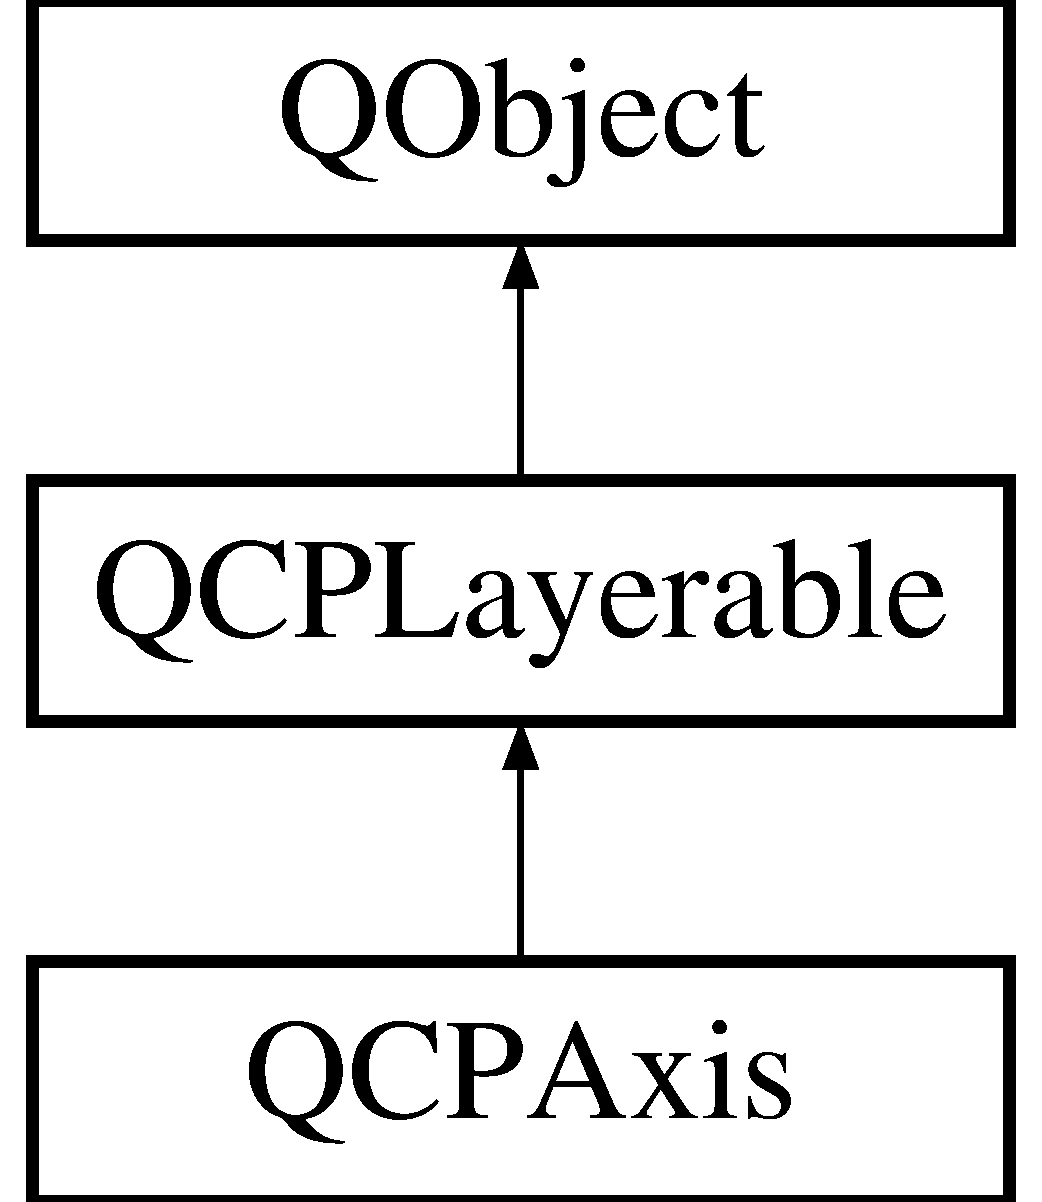
\includegraphics[height=3.000000cm]{class_q_c_p_axis}
\end{center}
\end{figure}
\subsection*{Public Types}
\begin{DoxyCompactItemize}
\item 
enum \hyperlink{class_q_c_p_axis_ae2bcc1728b382f10f064612b368bc18a}{Axis\+Type} \{ \hyperlink{class_q_c_p_axis_ae2bcc1728b382f10f064612b368bc18aaf84aa6cac6fb6099f54a2cbf7546b730}{at\+Left} = 0x01, 
\hyperlink{class_q_c_p_axis_ae2bcc1728b382f10f064612b368bc18aadf5509f7d29199ef2f263b1dd224b345}{at\+Right} = 0x02, 
\hyperlink{class_q_c_p_axis_ae2bcc1728b382f10f064612b368bc18aac0ece2b680d3f545e701f75af1655977}{at\+Top} = 0x04, 
\hyperlink{class_q_c_p_axis_ae2bcc1728b382f10f064612b368bc18aa220d68888516b6c3b493d144f1ba438f}{at\+Bottom} = 0x08
 \}
\item 
enum \hyperlink{class_q_c_p_axis_a4a7da0166f755f5abac23b765d184cad}{Label\+Type} \{ \hyperlink{class_q_c_p_axis_a4a7da0166f755f5abac23b765d184cada7f1eacf3b73adaefd334bea04e094b7e}{lt\+Number}, 
\hyperlink{class_q_c_p_axis_a4a7da0166f755f5abac23b765d184cadafc70594a9d877124dd11ccc187d4ac52}{lt\+Date\+Time}
 \}
\item 
enum \hyperlink{class_q_c_p_axis_a24b13374b9b8f75f47eed2ea78c37db9}{Label\+Side} \{ \hyperlink{class_q_c_p_axis_a24b13374b9b8f75f47eed2ea78c37db9aae7b027ac2839cf4ad611df30236fc3f}{ls\+Inside}, 
\hyperlink{class_q_c_p_axis_a24b13374b9b8f75f47eed2ea78c37db9a2eadb509fc0c9a8b35b85c86ec9f3c7a}{ls\+Outside}
 \}
\item 
enum \hyperlink{class_q_c_p_axis_a36d8e8658dbaa179bf2aeb973db2d6f0}{Scale\+Type} \{ \hyperlink{class_q_c_p_axis_a36d8e8658dbaa179bf2aeb973db2d6f0aff6e30a11a828bc850caffab0ff994f6}{st\+Linear}, 
\hyperlink{class_q_c_p_axis_a36d8e8658dbaa179bf2aeb973db2d6f0abf5b785ad976618816dc6f79b73216d4}{st\+Logarithmic}
 \}
\item 
enum \hyperlink{class_q_c_p_axis_abee4c7a54c468b1385dfce2c898b115f}{Selectable\+Part} \{ \hyperlink{class_q_c_p_axis_abee4c7a54c468b1385dfce2c898b115fae0df8123a5528d5ccf87cb7794f971ea}{sp\+None} = 0, 
\hyperlink{class_q_c_p_axis_abee4c7a54c468b1385dfce2c898b115fa8949d2c1a31eccae9be7ed32e7a1ae38}{sp\+Axis} = 0x001, 
\hyperlink{class_q_c_p_axis_abee4c7a54c468b1385dfce2c898b115fa584e0a3dc4d064880647619f4bd4e771}{sp\+Tick\+Labels} = 0x002, 
\hyperlink{class_q_c_p_axis_abee4c7a54c468b1385dfce2c898b115fa851e0600e0d08b4f5fee9361e3fedabd}{sp\+Axis\+Label} = 0x004
 \}
\end{DoxyCompactItemize}
\subsection*{Signals}
\begin{DoxyCompactItemize}
\item 
void \hyperlink{class_q_c_p_axis_af46d99613d29518795134ec4928e3873}{ticks\+Request} ()
\item 
void \hyperlink{class_q_c_p_axis_a0894084e4c16a1736534c4095746f910}{range\+Changed} (const \hyperlink{class_q_c_p_range}{Q\+C\+P\+Range} \&new\+Range)
\item 
void \hyperlink{class_q_c_p_axis_aac8576288e8e31f16186124bc10dd10d}{range\+Changed} (const \hyperlink{class_q_c_p_range}{Q\+C\+P\+Range} \&new\+Range, const \hyperlink{class_q_c_p_range}{Q\+C\+P\+Range} \&old\+Range)
\item 
void \hyperlink{class_q_c_p_axis_a3505ed8a93bd2e349d858d84996bf767}{scale\+Type\+Changed} (\hyperlink{class_q_c_p_axis_a36d8e8658dbaa179bf2aeb973db2d6f0}{Q\+C\+P\+Axis\+::\+Scale\+Type} scale\+Type)
\item 
void \hyperlink{class_q_c_p_axis_a62b598abeee7174a05f9d542cc85b1f5}{selection\+Changed} (const Q\+C\+P\+Axis\+::\+Selectable\+Parts \&parts)
\item 
void \hyperlink{class_q_c_p_axis_aa5ff1fd851139028a3bb4efcb31de9fc}{selectable\+Changed} (const Q\+C\+P\+Axis\+::\+Selectable\+Parts \&parts)
\end{DoxyCompactItemize}
\subsection*{Public Member Functions}
\begin{DoxyCompactItemize}
\item 
\hyperlink{class_q_c_p_axis_ac62c042968bae0e6d474fcfc57c9b71f}{Q\+C\+P\+Axis} (\hyperlink{class_q_c_p_axis_rect}{Q\+C\+P\+Axis\+Rect} $\ast$parent, \hyperlink{class_q_c_p_axis_ae2bcc1728b382f10f064612b368bc18a}{Axis\+Type} type)
\item 
\hypertarget{class_q_c_p_axis_aa19679359783c5ecd27757b7e5619976}{}\label{class_q_c_p_axis_aa19679359783c5ecd27757b7e5619976} 
\hyperlink{class_q_c_p_axis_ae2bcc1728b382f10f064612b368bc18a}{Axis\+Type} {\bfseries axis\+Type} () const
\item 
\hypertarget{class_q_c_p_axis_afc94bcfdf8adfe8e01013f13bdf159a2}{}\label{class_q_c_p_axis_afc94bcfdf8adfe8e01013f13bdf159a2} 
\hyperlink{class_q_c_p_axis_rect}{Q\+C\+P\+Axis\+Rect} $\ast$ {\bfseries axis\+Rect} () const
\item 
\hypertarget{class_q_c_p_axis_ad23e9ad97b44e9aeaf4fab8904280098}{}\label{class_q_c_p_axis_ad23e9ad97b44e9aeaf4fab8904280098} 
\hyperlink{class_q_c_p_axis_a36d8e8658dbaa179bf2aeb973db2d6f0}{Scale\+Type} {\bfseries scale\+Type} () const
\item 
\hypertarget{class_q_c_p_axis_a8f1cdf4b2b446db90adc7c1e2a826600}{}\label{class_q_c_p_axis_a8f1cdf4b2b446db90adc7c1e2a826600} 
double {\bfseries scale\+Log\+Base} () const
\item 
\hypertarget{class_q_c_p_axis_ac4058855a81f1a883cf2e754f6a6acb1}{}\label{class_q_c_p_axis_ac4058855a81f1a883cf2e754f6a6acb1} 
const \hyperlink{class_q_c_p_range}{Q\+C\+P\+Range} {\bfseries range} () const
\item 
\hypertarget{class_q_c_p_axis_ab9866dd1a78f1920f491ec12a794bec2}{}\label{class_q_c_p_axis_ab9866dd1a78f1920f491ec12a794bec2} 
bool {\bfseries range\+Reversed} () const
\item 
\hypertarget{class_q_c_p_axis_a2e377eff6e7f6529cc672901971721bd}{}\label{class_q_c_p_axis_a2e377eff6e7f6529cc672901971721bd} 
bool {\bfseries auto\+Ticks} () const
\item 
\hypertarget{class_q_c_p_axis_a3fe8fce237b74f4dc46154048b7187e7}{}\label{class_q_c_p_axis_a3fe8fce237b74f4dc46154048b7187e7} 
int {\bfseries auto\+Tick\+Count} () const
\item 
\hypertarget{class_q_c_p_axis_a999b064fe34031e2c91a87e95af76ee3}{}\label{class_q_c_p_axis_a999b064fe34031e2c91a87e95af76ee3} 
bool {\bfseries auto\+Tick\+Labels} () const
\item 
\hypertarget{class_q_c_p_axis_a1717c54da08abc29f406a0ff7da679f0}{}\label{class_q_c_p_axis_a1717c54da08abc29f406a0ff7da679f0} 
bool {\bfseries auto\+Tick\+Step} () const
\item 
\hypertarget{class_q_c_p_axis_ae3b171fb48bc48e430c6d00397782b58}{}\label{class_q_c_p_axis_ae3b171fb48bc48e430c6d00397782b58} 
bool {\bfseries auto\+Sub\+Ticks} () const
\item 
\hypertarget{class_q_c_p_axis_a5c3da767a2dc990f200856a9e27ea06e}{}\label{class_q_c_p_axis_a5c3da767a2dc990f200856a9e27ea06e} 
bool {\bfseries ticks} () const
\item 
\hypertarget{class_q_c_p_axis_ae4158bbc52939ee52cdb12b805860a28}{}\label{class_q_c_p_axis_ae4158bbc52939ee52cdb12b805860a28} 
bool {\bfseries tick\+Labels} () const
\item 
\hypertarget{class_q_c_p_axis_afac7316ca35941e7080f98e0022c1891}{}\label{class_q_c_p_axis_afac7316ca35941e7080f98e0022c1891} 
int {\bfseries tick\+Label\+Padding} () const
\item 
\hypertarget{class_q_c_p_axis_a0c66f78e18305dc5a7114757a5352f2b}{}\label{class_q_c_p_axis_a0c66f78e18305dc5a7114757a5352f2b} 
\hyperlink{class_q_c_p_axis_a4a7da0166f755f5abac23b765d184cad}{Label\+Type} {\bfseries tick\+Label\+Type} () const
\item 
\hypertarget{class_q_c_p_axis_a09f339b7125cf1094920f86687b88236}{}\label{class_q_c_p_axis_a09f339b7125cf1094920f86687b88236} 
Q\+Font {\bfseries tick\+Label\+Font} () const
\item 
\hypertarget{class_q_c_p_axis_a9e21b2326bb2de0b7a8efcd1efc0ce78}{}\label{class_q_c_p_axis_a9e21b2326bb2de0b7a8efcd1efc0ce78} 
Q\+Color {\bfseries tick\+Label\+Color} () const
\item 
\hypertarget{class_q_c_p_axis_a5c81e5d550266fdb9e11d96d1dc5713e}{}\label{class_q_c_p_axis_a5c81e5d550266fdb9e11d96d1dc5713e} 
double {\bfseries tick\+Label\+Rotation} () const
\item 
\hypertarget{class_q_c_p_axis_a1dc21783965a7c7d9c29c2a75d0a54e1}{}\label{class_q_c_p_axis_a1dc21783965a7c7d9c29c2a75d0a54e1} 
\hyperlink{class_q_c_p_axis_a24b13374b9b8f75f47eed2ea78c37db9}{Label\+Side} {\bfseries tick\+Label\+Side} () const
\item 
\hypertarget{class_q_c_p_axis_a2ba678e9e69969b910c4790a772f6bea}{}\label{class_q_c_p_axis_a2ba678e9e69969b910c4790a772f6bea} 
Q\+String {\bfseries date\+Time\+Format} () const
\item 
\hypertarget{class_q_c_p_axis_aea1341545f772173451671744e50ea22}{}\label{class_q_c_p_axis_aea1341545f772173451671744e50ea22} 
Qt\+::\+Time\+Spec {\bfseries date\+Time\+Spec} () const
\item 
\hypertarget{class_q_c_p_axis_a20cc29c2f282a0e9efd8f32145e47be6}{}\label{class_q_c_p_axis_a20cc29c2f282a0e9efd8f32145e47be6} 
Q\+String {\bfseries number\+Format} () const
\item 
\hypertarget{class_q_c_p_axis_a2562b6f3a4a01c7ed83a388042664998}{}\label{class_q_c_p_axis_a2562b6f3a4a01c7ed83a388042664998} 
int {\bfseries number\+Precision} () const
\item 
\hypertarget{class_q_c_p_axis_a951320db20b7add3dc30853fcbf3b520}{}\label{class_q_c_p_axis_a951320db20b7add3dc30853fcbf3b520} 
double {\bfseries tick\+Step} () const
\item 
\hypertarget{class_q_c_p_axis_a5aad9d6b34821ab0751dfc38dbc92a46}{}\label{class_q_c_p_axis_a5aad9d6b34821ab0751dfc38dbc92a46} 
Q\+Vector$<$ double $>$ {\bfseries tick\+Vector} () const
\item 
\hypertarget{class_q_c_p_axis_a1bd4a9036e0c9fc68b6f3df81f07e55f}{}\label{class_q_c_p_axis_a1bd4a9036e0c9fc68b6f3df81f07e55f} 
Q\+Vector$<$ Q\+String $>$ {\bfseries tick\+Vector\+Labels} () const
\item 
\hypertarget{class_q_c_p_axis_ace2accb350fd3f3f474280f58c1d61c5}{}\label{class_q_c_p_axis_ace2accb350fd3f3f474280f58c1d61c5} 
int {\bfseries tick\+Length\+In} () const
\item 
\hypertarget{class_q_c_p_axis_ad3ba6614ccddf351f133e0acdd4f021e}{}\label{class_q_c_p_axis_ad3ba6614ccddf351f133e0acdd4f021e} 
int {\bfseries tick\+Length\+Out} () const
\item 
\hypertarget{class_q_c_p_axis_aba4695601f385cb4fe48b7d0dfa4efb9}{}\label{class_q_c_p_axis_aba4695601f385cb4fe48b7d0dfa4efb9} 
int {\bfseries sub\+Tick\+Count} () const
\item 
\hypertarget{class_q_c_p_axis_af907c8ecc4624d1bf4a8f6f702e64fbe}{}\label{class_q_c_p_axis_af907c8ecc4624d1bf4a8f6f702e64fbe} 
int {\bfseries sub\+Tick\+Length\+In} () const
\item 
\hypertarget{class_q_c_p_axis_ac98c66cae50c98f3ae90e2969382976d}{}\label{class_q_c_p_axis_ac98c66cae50c98f3ae90e2969382976d} 
int {\bfseries sub\+Tick\+Length\+Out} () const
\item 
\hypertarget{class_q_c_p_axis_a216974be018e73008b3cf6d033c1325d}{}\label{class_q_c_p_axis_a216974be018e73008b3cf6d033c1325d} 
Q\+Pen {\bfseries base\+Pen} () const
\item 
\hypertarget{class_q_c_p_axis_affd022d4f56dfc575b4ced95ad417860}{}\label{class_q_c_p_axis_affd022d4f56dfc575b4ced95ad417860} 
Q\+Pen {\bfseries tick\+Pen} () const
\item 
\hypertarget{class_q_c_p_axis_a7a89df74ba427fac311bf4cc92fbddca}{}\label{class_q_c_p_axis_a7a89df74ba427fac311bf4cc92fbddca} 
Q\+Pen {\bfseries sub\+Tick\+Pen} () const
\item 
\hypertarget{class_q_c_p_axis_aa7b465fe233f1878793954ba5ab9c47e}{}\label{class_q_c_p_axis_aa7b465fe233f1878793954ba5ab9c47e} 
Q\+Font {\bfseries label\+Font} () const
\item 
\hypertarget{class_q_c_p_axis_a05794f13d322da7fd9d5554d11186b0e}{}\label{class_q_c_p_axis_a05794f13d322da7fd9d5554d11186b0e} 
Q\+Color {\bfseries label\+Color} () const
\item 
\hypertarget{class_q_c_p_axis_a32ba4d3effcddd8af3bc49f405e1d53e}{}\label{class_q_c_p_axis_a32ba4d3effcddd8af3bc49f405e1d53e} 
Q\+String {\bfseries label} () const
\item 
\hypertarget{class_q_c_p_axis_a6d9a9fe1c7166f209fb1e25686390451}{}\label{class_q_c_p_axis_a6d9a9fe1c7166f209fb1e25686390451} 
int {\bfseries label\+Padding} () const
\item 
\hypertarget{class_q_c_p_axis_a07df379d5c017b8f3a4702532eb037b2}{}\label{class_q_c_p_axis_a07df379d5c017b8f3a4702532eb037b2} 
int {\bfseries padding} () const
\item 
\hypertarget{class_q_c_p_axis_aef66fa16353b4993b1cceabfb644a1a9}{}\label{class_q_c_p_axis_aef66fa16353b4993b1cceabfb644a1a9} 
int {\bfseries offset} () const
\item 
\hypertarget{class_q_c_p_axis_a893e8d6cfed9267eb2b793cb1d2b4dce}{}\label{class_q_c_p_axis_a893e8d6cfed9267eb2b793cb1d2b4dce} 
Selectable\+Parts {\bfseries selected\+Parts} () const
\item 
\hypertarget{class_q_c_p_axis_a1d12d157756c114f4e57517c62177181}{}\label{class_q_c_p_axis_a1d12d157756c114f4e57517c62177181} 
Selectable\+Parts {\bfseries selectable\+Parts} () const
\item 
\hypertarget{class_q_c_p_axis_a09817512bef8ddfb669a6828f9c855bc}{}\label{class_q_c_p_axis_a09817512bef8ddfb669a6828f9c855bc} 
Q\+Font {\bfseries selected\+Tick\+Label\+Font} () const
\item 
\hypertarget{class_q_c_p_axis_a1399d614f7c307159bfec938a069203d}{}\label{class_q_c_p_axis_a1399d614f7c307159bfec938a069203d} 
Q\+Font {\bfseries selected\+Label\+Font} () const
\item 
\hypertarget{class_q_c_p_axis_a75f11d3031a11559f3e984e916fcde2c}{}\label{class_q_c_p_axis_a75f11d3031a11559f3e984e916fcde2c} 
Q\+Color {\bfseries selected\+Tick\+Label\+Color} () const
\item 
\hypertarget{class_q_c_p_axis_a7adea64ef4b715e7a1c519fff2b110b8}{}\label{class_q_c_p_axis_a7adea64ef4b715e7a1c519fff2b110b8} 
Q\+Color {\bfseries selected\+Label\+Color} () const
\item 
\hypertarget{class_q_c_p_axis_a0d54314ab3053fd0fb77294a0e7f08cb}{}\label{class_q_c_p_axis_a0d54314ab3053fd0fb77294a0e7f08cb} 
Q\+Pen {\bfseries selected\+Base\+Pen} () const
\item 
\hypertarget{class_q_c_p_axis_a76b52a6d824ccf9a95eb024251e1b833}{}\label{class_q_c_p_axis_a76b52a6d824ccf9a95eb024251e1b833} 
Q\+Pen {\bfseries selected\+Tick\+Pen} () const
\item 
\hypertarget{class_q_c_p_axis_a73c147bb2c5598edbb842adc2da8a7bf}{}\label{class_q_c_p_axis_a73c147bb2c5598edbb842adc2da8a7bf} 
Q\+Pen {\bfseries selected\+Sub\+Tick\+Pen} () const
\item 
\hypertarget{class_q_c_p_axis_a0cc60e5694ed4df6a2c3554e53ee6ae7}{}\label{class_q_c_p_axis_a0cc60e5694ed4df6a2c3554e53ee6ae7} 
\hyperlink{class_q_c_p_line_ending}{Q\+C\+P\+Line\+Ending} {\bfseries lower\+Ending} () const
\item 
\hypertarget{class_q_c_p_axis_a9feaf5f78286693e89221bc205f9389a}{}\label{class_q_c_p_axis_a9feaf5f78286693e89221bc205f9389a} 
\hyperlink{class_q_c_p_line_ending}{Q\+C\+P\+Line\+Ending} {\bfseries upper\+Ending} () const
\item 
\hyperlink{class_q_c_p_grid}{Q\+C\+P\+Grid} $\ast$ \hyperlink{class_q_c_p_axis_a63f1dd2df663680d2a8d06c19592dd63}{grid} () const
\item 
Q\+\_\+\+S\+L\+OT void \hyperlink{class_q_c_p_axis_adef29cae617af4f519f6c40d1a866ca6}{set\+Scale\+Type} (\hyperlink{class_q_c_p_axis_a36d8e8658dbaa179bf2aeb973db2d6f0}{Q\+C\+P\+Axis\+::\+Scale\+Type} type)
\item 
void \hyperlink{class_q_c_p_axis_a726186054be90487885a748aa1b42188}{set\+Scale\+Log\+Base} (double base)
\item 
Q\+\_\+\+S\+L\+OT void \hyperlink{class_q_c_p_axis_aebdfea5d44c3a0ad2b4700cd4d25b641}{set\+Range} (const \hyperlink{class_q_c_p_range}{Q\+C\+P\+Range} \&range)
\item 
void \hyperlink{class_q_c_p_axis_a57d6ee9e9009fe88cb19db476ec70bca}{set\+Range} (double lower, double upper)
\item 
void \hyperlink{class_q_c_p_axis_acf60e5b2d631fbc8c4548c3d579cb6d0}{set\+Range} (double position, double size, Qt\+::\+Alignment\+Flag alignment)
\item 
void \hyperlink{class_q_c_p_axis_afcf51227d337db28d1a9ce9a4d1bc91a}{set\+Range\+Lower} (double lower)
\item 
void \hyperlink{class_q_c_p_axis_acd3ca1247aa867b540cd5ec30ccd3bef}{set\+Range\+Upper} (double upper)
\item 
void \hyperlink{class_q_c_p_axis_a2172fdb196b1a0dc3f40992fcad8e9e1}{set\+Range\+Reversed} (bool reversed)
\item 
void \hyperlink{class_q_c_p_axis_ae867c23d3a6a7bd4d09cc66c5d018f63}{set\+Auto\+Ticks} (bool on)
\item 
void \hyperlink{class_q_c_p_axis_a7c7111cbeac9ec5fcb40f93a1ef51a0b}{set\+Auto\+Tick\+Count} (int approximate\+Count)
\item 
void \hyperlink{class_q_c_p_axis_aaa47e3a6bac0c20d4beb9028f01bc1a1}{set\+Auto\+Tick\+Labels} (bool on)
\item 
void \hyperlink{class_q_c_p_axis_a99fe77b034e06f5b723995beab96e741}{set\+Auto\+Tick\+Step} (bool on)
\item 
void \hyperlink{class_q_c_p_axis_adcbdec7a60054b88571e89599f4a45bf}{set\+Auto\+Sub\+Ticks} (bool on)
\item 
void \hyperlink{class_q_c_p_axis_ac891409315bc379e3b1abdb162c1a011}{set\+Ticks} (bool show)
\item 
void \hyperlink{class_q_c_p_axis_a04ba16e1f6f78d70f938519576ed32c8}{set\+Tick\+Labels} (bool show)
\item 
void \hyperlink{class_q_c_p_axis_af302c479af9dbc2e9f0e44e07c0012ee}{set\+Tick\+Label\+Padding} (int padding)
\item 
void \hyperlink{class_q_c_p_axis_a54f24f5ce8feea25209388a863d7e448}{set\+Tick\+Label\+Type} (\hyperlink{class_q_c_p_axis_a4a7da0166f755f5abac23b765d184cad}{Label\+Type} type)
\item 
void \hyperlink{class_q_c_p_axis_a2b8690c4e8dbc39d9185d2b398ce7a6c}{set\+Tick\+Label\+Font} (const Q\+Font \&font)
\item 
void \hyperlink{class_q_c_p_axis_a395e445c3fe496b935bee7b911ecfd1c}{set\+Tick\+Label\+Color} (const Q\+Color \&color)
\item 
void \hyperlink{class_q_c_p_axis_a1bddd4413df8a576b7ad4b067fb33375}{set\+Tick\+Label\+Rotation} (double degrees)
\item 
void \hyperlink{class_q_c_p_axis_a13ec644fc6e22715744c92c6dfa4f0fa}{set\+Tick\+Label\+Side} (\hyperlink{class_q_c_p_axis_a24b13374b9b8f75f47eed2ea78c37db9}{Label\+Side} side)
\item 
void \hyperlink{class_q_c_p_axis_a2ee0191daa03524a682113e63e05f7a7}{set\+Date\+Time\+Format} (const Q\+String \&format)
\item 
void \hyperlink{class_q_c_p_axis_a262e06731debed7eee11fa6a81d67eaf}{set\+Date\+Time\+Spec} (const Qt\+::\+Time\+Spec \&time\+Spec)
\item 
void \hyperlink{class_q_c_p_axis_ae585a54dc2aac662e90a2ca82f002590}{set\+Number\+Format} (const Q\+String \&format\+Code)
\item 
void \hyperlink{class_q_c_p_axis_a21dc8023ad7500382ad9574b48137e63}{set\+Number\+Precision} (int precision)
\item 
void \hyperlink{class_q_c_p_axis_af727db0acc6492c4c774c0700e738205}{set\+Tick\+Step} (double step)
\item 
void \hyperlink{class_q_c_p_axis_a871db94c5d796c80fcbe1a9d4506e27e}{set\+Tick\+Vector} (const Q\+Vector$<$ double $>$ \&vec)
\item 
void \hyperlink{class_q_c_p_axis_a921d3ba3853ca3bd2cce3459f7a243ed}{set\+Tick\+Vector\+Labels} (const Q\+Vector$<$ Q\+String $>$ \&vec)
\item 
void \hyperlink{class_q_c_p_axis_a62ec40bebe3540e9c1479a8fd2be3b0d}{set\+Tick\+Length} (int inside, int outside=0)
\item 
void \hyperlink{class_q_c_p_axis_afae1a37a99611366275a51204d991739}{set\+Tick\+Length\+In} (int inside)
\item 
void \hyperlink{class_q_c_p_axis_a3b8a0debd1ffedd2c22d0592dfbb4e62}{set\+Tick\+Length\+Out} (int outside)
\item 
void \hyperlink{class_q_c_p_axis_a4b1554ead9d7f9799650d51383e326dd}{set\+Sub\+Tick\+Count} (int count)
\item 
void \hyperlink{class_q_c_p_axis_ab702d6fd42fc620607435339a1c2a2e1}{set\+Sub\+Tick\+Length} (int inside, int outside=0)
\item 
void \hyperlink{class_q_c_p_axis_ac46fa2a993a9f5789540977610acf1de}{set\+Sub\+Tick\+Length\+In} (int inside)
\item 
void \hyperlink{class_q_c_p_axis_a4c6dfc3963492ed72a77724012df5f23}{set\+Sub\+Tick\+Length\+Out} (int outside)
\item 
void \hyperlink{class_q_c_p_axis_a778d45fb71b3c7ab3bb7079e18b058e4}{set\+Base\+Pen} (const Q\+Pen \&pen)
\item 
void \hyperlink{class_q_c_p_axis_ad80923bcc1c5da4c4db602c5325e797e}{set\+Tick\+Pen} (const Q\+Pen \&pen)
\item 
void \hyperlink{class_q_c_p_axis_aede4028ae7516bd51a60618a8233f9cf}{set\+Sub\+Tick\+Pen} (const Q\+Pen \&pen)
\item 
void \hyperlink{class_q_c_p_axis_a71ac1a47f7547e490a8c4311d1433cf3}{set\+Label\+Font} (const Q\+Font \&font)
\item 
void \hyperlink{class_q_c_p_axis_a6c906fe56d75f0122335b9f79b999608}{set\+Label\+Color} (const Q\+Color \&color)
\item 
void \hyperlink{class_q_c_p_axis_a33bcc382c111c9f31bb0687352a2dea4}{set\+Label} (const Q\+String \&str)
\item 
void \hyperlink{class_q_c_p_axis_a4391192a766e5d20cfe5cbc17607a7a2}{set\+Label\+Padding} (int padding)
\item 
void \hyperlink{class_q_c_p_axis_a5691441cb3de9e9844855d339c0db279}{set\+Padding} (int padding)
\item 
void \hyperlink{class_q_c_p_axis_a04a652603cbe50eba9969ee6d68873c3}{set\+Offset} (int offset)
\item 
void \hyperlink{class_q_c_p_axis_a845ccb560b7bc5281098a5be494145f6}{set\+Selected\+Tick\+Label\+Font} (const Q\+Font \&font)
\item 
void \hyperlink{class_q_c_p_axis_a02ec2a75d4d8401eaab834fbc6803d30}{set\+Selected\+Label\+Font} (const Q\+Font \&font)
\item 
void \hyperlink{class_q_c_p_axis_a9bdbf5e63ab15187f3a1de9440129227}{set\+Selected\+Tick\+Label\+Color} (const Q\+Color \&color)
\item 
void \hyperlink{class_q_c_p_axis_a5d502dec597c634f491fdd73d151c72d}{set\+Selected\+Label\+Color} (const Q\+Color \&color)
\item 
void \hyperlink{class_q_c_p_axis_aeb917a909215605b95ef2be843de1ee8}{set\+Selected\+Base\+Pen} (const Q\+Pen \&pen)
\item 
void \hyperlink{class_q_c_p_axis_a8360502685eb782edbf04019c9345cdc}{set\+Selected\+Tick\+Pen} (const Q\+Pen \&pen)
\item 
void \hyperlink{class_q_c_p_axis_a2a00a7166600155eac26843132eb9576}{set\+Selected\+Sub\+Tick\+Pen} (const Q\+Pen \&pen)
\item 
Q\+\_\+\+S\+L\+OT void \hyperlink{class_q_c_p_axis_a513f9b9e326c505d9bec54880031b085}{set\+Selectable\+Parts} (const Q\+C\+P\+Axis\+::\+Selectable\+Parts \&selectable\+Parts)
\item 
Q\+\_\+\+S\+L\+OT void \hyperlink{class_q_c_p_axis_ab9d7a69277dcbed9119b3c1f25ca19c3}{set\+Selected\+Parts} (const Q\+C\+P\+Axis\+::\+Selectable\+Parts \&selected\+Parts)
\item 
void \hyperlink{class_q_c_p_axis_a08af1c72db9ae4dc8cb8a973d44405ab}{set\+Lower\+Ending} (const \hyperlink{class_q_c_p_line_ending}{Q\+C\+P\+Line\+Ending} \&ending)
\item 
void \hyperlink{class_q_c_p_axis_a69119b892fc306f651763596685aa377}{set\+Upper\+Ending} (const \hyperlink{class_q_c_p_line_ending}{Q\+C\+P\+Line\+Ending} \&ending)
\item 
virtual double \hyperlink{class_q_c_p_axis_a48e4f1bafd1826ba2ad46b691205bb90}{select\+Test} (const Q\+PointF \&pos, bool only\+Selectable, Q\+Variant $\ast$details=0) const
\item 
Qt\+::\+Orientation \hyperlink{class_q_c_p_axis_ab988ef4538e2655bb77bd138189cd42e}{orientation} () const
\item 
void \hyperlink{class_q_c_p_axis_a18f3a68f2b691af1fd34b6593c886630}{move\+Range} (double diff)
\item 
void \hyperlink{class_q_c_p_axis_a7072ff96fe690148f1bbcdb4f773ea1c}{scale\+Range} (double factor, double center)
\item 
void \hyperlink{class_q_c_p_axis_af4bbd446dcaee5a83ac30ce9bcd6e125}{set\+Scale\+Ratio} (const \hyperlink{class_q_c_p_axis}{Q\+C\+P\+Axis} $\ast$other\+Axis, double ratio=1.\+0)
\item 
void \hyperlink{class_q_c_p_axis_a499345f02ebce4b23d8ccec96e58daa9}{rescale} (bool only\+Visible\+Plottables=false)
\item 
double \hyperlink{class_q_c_p_axis_a536ef8f624cac59b6b6fdcb495723c57}{pixel\+To\+Coord} (double value) const
\item 
double \hyperlink{class_q_c_p_axis_af15d1b3a7f7e9b53d759d3ccff1fe4b4}{coord\+To\+Pixel} (double value) const
\item 
\hyperlink{class_q_c_p_axis_abee4c7a54c468b1385dfce2c898b115f}{Selectable\+Part} \hyperlink{class_q_c_p_axis_a22ab2d71d7341b9b3974c0dd10619af2}{get\+Part\+At} (const Q\+PointF \&pos) const
\item 
Q\+List$<$ \hyperlink{class_q_c_p_abstract_plottable}{Q\+C\+P\+Abstract\+Plottable} $\ast$ $>$ \hyperlink{class_q_c_p_axis_ac5e0f6f65c75efb5fd32275d6e4ef0d6}{plottables} () const
\item 
Q\+List$<$ \hyperlink{class_q_c_p_graph}{Q\+C\+P\+Graph} $\ast$ $>$ \hyperlink{class_q_c_p_axis_ad590c0da223697a2727f97a520870fec}{graphs} () const
\item 
Q\+List$<$ \hyperlink{class_q_c_p_abstract_item}{Q\+C\+P\+Abstract\+Item} $\ast$ $>$ \hyperlink{class_q_c_p_axis_a42761bc68e2f3a9f68549d45b73f705b}{items} () const
\end{DoxyCompactItemize}
\subsection*{Static Public Member Functions}
\begin{DoxyCompactItemize}
\item 
static \hyperlink{class_q_c_p_axis_ae2bcc1728b382f10f064612b368bc18a}{Axis\+Type} \hyperlink{class_q_c_p_axis_ac0a6b77bd52bec6c81cd62d167cfeba6}{margin\+Side\+To\+Axis\+Type} (\hyperlink{namespace_q_c_p_a7e487e3e2ccb62ab7771065bab7cae54}{Q\+C\+P\+::\+Margin\+Side} side)
\item 
static Qt\+::\+Orientation \hyperlink{class_q_c_p_axis_a9a68b3e45f1b1e33d4d807822342516c}{orientation} (\hyperlink{class_q_c_p_axis_ae2bcc1728b382f10f064612b368bc18a}{Axis\+Type} type)
\item 
static \hyperlink{class_q_c_p_axis_ae2bcc1728b382f10f064612b368bc18a}{Axis\+Type} \hyperlink{class_q_c_p_axis_aa85ba73dfee6483e23825461b725e363}{opposite} (\hyperlink{class_q_c_p_axis_ae2bcc1728b382f10f064612b368bc18a}{Axis\+Type} type)
\end{DoxyCompactItemize}
\subsection*{Protected Member Functions}
\begin{DoxyCompactItemize}
\item 
\hypertarget{class_q_c_p_axis_a57d9e961bae7d62f5b4e1f143e660c78}{}\label{class_q_c_p_axis_a57d9e961bae7d62f5b4e1f143e660c78} 
virtual void {\bfseries setup\+Tick\+Vectors} ()
\item 
\hypertarget{class_q_c_p_axis_a626eef437c874148df1a5ac78506d463}{}\label{class_q_c_p_axis_a626eef437c874148df1a5ac78506d463} 
virtual void {\bfseries generate\+Auto\+Ticks} ()
\item 
\hypertarget{class_q_c_p_axis_aca96dda6dbd08b062fc96e34df16c68a}{}\label{class_q_c_p_axis_aca96dda6dbd08b062fc96e34df16c68a} 
virtual int {\bfseries calculate\+Auto\+Sub\+Tick\+Count} (double tick\+Step) const
\item 
\hypertarget{class_q_c_p_axis_a47bdb0a55de6759489ee47665199aebb}{}\label{class_q_c_p_axis_a47bdb0a55de6759489ee47665199aebb} 
virtual int {\bfseries calculate\+Margin} ()
\item 
\hypertarget{class_q_c_p_axis_a427f3de3369a8691ffece384437f0c7a}{}\label{class_q_c_p_axis_a427f3de3369a8691ffece384437f0c7a} 
virtual void {\bfseries apply\+Default\+Antialiasing\+Hint} (\hyperlink{class_q_c_p_painter}{Q\+C\+P\+Painter} $\ast$painter) const
\item 
\hypertarget{class_q_c_p_axis_a258b1e783eda5cd14ec5552c696a424e}{}\label{class_q_c_p_axis_a258b1e783eda5cd14ec5552c696a424e} 
virtual void {\bfseries draw} (\hyperlink{class_q_c_p_painter}{Q\+C\+P\+Painter} $\ast$painter)
\item 
\hypertarget{class_q_c_p_axis_a04b897f3e24724b8f021639b220fd71c}{}\label{class_q_c_p_axis_a04b897f3e24724b8f021639b220fd71c} 
virtual \hyperlink{namespace_q_c_p_a2ad6bb6281c7c2d593d4277b44c2b037}{Q\+C\+P\+::\+Interaction} {\bfseries selection\+Category} () const
\item 
\hypertarget{class_q_c_p_axis_aa8a5fe80e2898ec08ada26b5fbee9eca}{}\label{class_q_c_p_axis_aa8a5fe80e2898ec08ada26b5fbee9eca} 
virtual void {\bfseries select\+Event} (Q\+Mouse\+Event $\ast$event, bool additive, const Q\+Variant \&details, bool $\ast$selection\+State\+Changed)
\item 
\hypertarget{class_q_c_p_axis_a53512242cde6ec21943a3ba10dbf78c3}{}\label{class_q_c_p_axis_a53512242cde6ec21943a3ba10dbf78c3} 
virtual void {\bfseries deselect\+Event} (bool $\ast$selection\+State\+Changed)
\item 
\hypertarget{class_q_c_p_axis_aeda1feaedaabc6e0f0d5b0c18a3898d2}{}\label{class_q_c_p_axis_aeda1feaedaabc6e0f0d5b0c18a3898d2} 
void {\bfseries visible\+Tick\+Bounds} (int \&low\+Index, int \&high\+Index) const
\item 
\hypertarget{class_q_c_p_axis_ae759538b7eeb12259944e75a6bc359da}{}\label{class_q_c_p_axis_ae759538b7eeb12259944e75a6bc359da} 
double {\bfseries base\+Log} (double value) const
\item 
\hypertarget{class_q_c_p_axis_aaa91530d01736d9b84dd91c1e8a26d56}{}\label{class_q_c_p_axis_aaa91530d01736d9b84dd91c1e8a26d56} 
double {\bfseries base\+Pow} (double value) const
\item 
\hypertarget{class_q_c_p_axis_a8cd3764c6a4ce9c3d7d913e81cad0a50}{}\label{class_q_c_p_axis_a8cd3764c6a4ce9c3d7d913e81cad0a50} 
Q\+Pen {\bfseries get\+Base\+Pen} () const
\item 
\hypertarget{class_q_c_p_axis_afe7d57415cbbf31e5549a5cc40b6f8d8}{}\label{class_q_c_p_axis_afe7d57415cbbf31e5549a5cc40b6f8d8} 
Q\+Pen {\bfseries get\+Tick\+Pen} () const
\item 
\hypertarget{class_q_c_p_axis_aad7739c229b292ddab0b3a43a5676f54}{}\label{class_q_c_p_axis_aad7739c229b292ddab0b3a43a5676f54} 
Q\+Pen {\bfseries get\+Sub\+Tick\+Pen} () const
\item 
\hypertarget{class_q_c_p_axis_a694ab8b4240f3c90a866372e3dcb364f}{}\label{class_q_c_p_axis_a694ab8b4240f3c90a866372e3dcb364f} 
Q\+Font {\bfseries get\+Tick\+Label\+Font} () const
\item 
\hypertarget{class_q_c_p_axis_aeac21c907d2516af9cde9a463043d671}{}\label{class_q_c_p_axis_aeac21c907d2516af9cde9a463043d671} 
Q\+Font {\bfseries get\+Label\+Font} () const
\item 
\hypertarget{class_q_c_p_axis_a8d00d5b78ecfbebbea5a8161bddb9a17}{}\label{class_q_c_p_axis_a8d00d5b78ecfbebbea5a8161bddb9a17} 
Q\+Color {\bfseries get\+Tick\+Label\+Color} () const
\item 
\hypertarget{class_q_c_p_axis_ae914abd56afa570cb9f2ab50e59c0f0e}{}\label{class_q_c_p_axis_ae914abd56afa570cb9f2ab50e59c0f0e} 
Q\+Color {\bfseries get\+Label\+Color} () const
\end{DoxyCompactItemize}
\subsection*{Protected Attributes}
\begin{DoxyCompactItemize}
\item 
\hypertarget{class_q_c_p_axis_ae704bf9f2c2b026f08dd4ccad79c616e}{}\label{class_q_c_p_axis_ae704bf9f2c2b026f08dd4ccad79c616e} 
\hyperlink{class_q_c_p_axis_ae2bcc1728b382f10f064612b368bc18a}{Axis\+Type} {\bfseries m\+Axis\+Type}
\item 
\hypertarget{class_q_c_p_axis_a6f150b65a202f32936997960e331dfcb}{}\label{class_q_c_p_axis_a6f150b65a202f32936997960e331dfcb} 
\hyperlink{class_q_c_p_axis_rect}{Q\+C\+P\+Axis\+Rect} $\ast$ {\bfseries m\+Axis\+Rect}
\item 
\hypertarget{class_q_c_p_axis_a52a805a4f03231210e0880db7f77e098}{}\label{class_q_c_p_axis_a52a805a4f03231210e0880db7f77e098} 
int {\bfseries m\+Padding}
\item 
\hypertarget{class_q_c_p_axis_a048e1792fa86f4f86df55200b3f0be36}{}\label{class_q_c_p_axis_a048e1792fa86f4f86df55200b3f0be36} 
Qt\+::\+Orientation {\bfseries m\+Orientation}
\item 
\hypertarget{class_q_c_p_axis_ab9042d8a095998f27a28b39411d8b9c3}{}\label{class_q_c_p_axis_ab9042d8a095998f27a28b39411d8b9c3} 
Selectable\+Parts {\bfseries m\+Selectable\+Parts}
\item 
\hypertarget{class_q_c_p_axis_a8f1eb0abfe2ae64652aa46b360e841e4}{}\label{class_q_c_p_axis_a8f1eb0abfe2ae64652aa46b360e841e4} 
Selectable\+Parts {\bfseries m\+Selected\+Parts}
\item 
\hypertarget{class_q_c_p_axis_ad6b4a0aee9558fb35529e960b8fef72d}{}\label{class_q_c_p_axis_ad6b4a0aee9558fb35529e960b8fef72d} 
Q\+Pen {\bfseries m\+Base\+Pen}
\item 
\hypertarget{class_q_c_p_axis_a80baa4e3c16f9b6edf3eccacd2a50fde}{}\label{class_q_c_p_axis_a80baa4e3c16f9b6edf3eccacd2a50fde} 
Q\+Pen {\bfseries m\+Selected\+Base\+Pen}
\item 
\hypertarget{class_q_c_p_axis_ae8001dbdfc47685c1cf7b98b044460e6}{}\label{class_q_c_p_axis_ae8001dbdfc47685c1cf7b98b044460e6} 
Q\+String {\bfseries m\+Label}
\item 
\hypertarget{class_q_c_p_axis_a37442d470e30e19b81ecaf979a34d046}{}\label{class_q_c_p_axis_a37442d470e30e19b81ecaf979a34d046} 
Q\+Font {\bfseries m\+Label\+Font}
\item 
\hypertarget{class_q_c_p_axis_ae48fe3489afadc0b3cd003233e2bf19f}{}\label{class_q_c_p_axis_ae48fe3489afadc0b3cd003233e2bf19f} 
Q\+Font {\bfseries m\+Selected\+Label\+Font}
\item 
\hypertarget{class_q_c_p_axis_a457a003bb1c2b6ab73e5a173ba7558fd}{}\label{class_q_c_p_axis_a457a003bb1c2b6ab73e5a173ba7558fd} 
Q\+Color {\bfseries m\+Label\+Color}
\item 
\hypertarget{class_q_c_p_axis_a94f57de3ba024471ca206d83cf2258dd}{}\label{class_q_c_p_axis_a94f57de3ba024471ca206d83cf2258dd} 
Q\+Color {\bfseries m\+Selected\+Label\+Color}
\item 
\hypertarget{class_q_c_p_axis_a3e4315be072026644e69009557a2fa11}{}\label{class_q_c_p_axis_a3e4315be072026644e69009557a2fa11} 
bool {\bfseries m\+Tick\+Labels}
\item 
\hypertarget{class_q_c_p_axis_a721e496b342f272078c5ff84564e472f}{}\label{class_q_c_p_axis_a721e496b342f272078c5ff84564e472f} 
bool {\bfseries m\+Auto\+Tick\+Labels}
\item 
\hypertarget{class_q_c_p_axis_a6e056c1cb1aab0eddebfebbcb78c8f90}{}\label{class_q_c_p_axis_a6e056c1cb1aab0eddebfebbcb78c8f90} 
\hyperlink{class_q_c_p_axis_a4a7da0166f755f5abac23b765d184cad}{Label\+Type} {\bfseries m\+Tick\+Label\+Type}
\item 
\hypertarget{class_q_c_p_axis_add79d1e39c4ed65869a1e9cc79043f3f}{}\label{class_q_c_p_axis_add79d1e39c4ed65869a1e9cc79043f3f} 
Q\+Font {\bfseries m\+Tick\+Label\+Font}
\item 
\hypertarget{class_q_c_p_axis_a4f2e4919da9615dac612662c249b1119}{}\label{class_q_c_p_axis_a4f2e4919da9615dac612662c249b1119} 
Q\+Font {\bfseries m\+Selected\+Tick\+Label\+Font}
\item 
\hypertarget{class_q_c_p_axis_a6384a749b3b56a97df081d8082321ab4}{}\label{class_q_c_p_axis_a6384a749b3b56a97df081d8082321ab4} 
Q\+Color {\bfseries m\+Tick\+Label\+Color}
\item 
\hypertarget{class_q_c_p_axis_a3bcad40902f45dc4c991a2c3e4d31d70}{}\label{class_q_c_p_axis_a3bcad40902f45dc4c991a2c3e4d31d70} 
Q\+Color {\bfseries m\+Selected\+Tick\+Label\+Color}
\item 
\hypertarget{class_q_c_p_axis_a0b7ad83550d71daab4cfee2918e168e0}{}\label{class_q_c_p_axis_a0b7ad83550d71daab4cfee2918e168e0} 
Q\+String {\bfseries m\+Date\+Time\+Format}
\item 
\hypertarget{class_q_c_p_axis_af73bec228c1a3203dc8aef1e84a46759}{}\label{class_q_c_p_axis_af73bec228c1a3203dc8aef1e84a46759} 
Qt\+::\+Time\+Spec {\bfseries m\+Date\+Time\+Spec}
\item 
\hypertarget{class_q_c_p_axis_acd76e8c783384d99ccc4a13797eec188}{}\label{class_q_c_p_axis_acd76e8c783384d99ccc4a13797eec188} 
int {\bfseries m\+Number\+Precision}
\item 
\hypertarget{class_q_c_p_axis_a39594313deef458f425bba25cd337a8a}{}\label{class_q_c_p_axis_a39594313deef458f425bba25cd337a8a} 
Q\+Latin1\+Char {\bfseries m\+Number\+Format\+Char}
\item 
\hypertarget{class_q_c_p_axis_af03809bee3f3e35fcc38d25b6dd5003b}{}\label{class_q_c_p_axis_af03809bee3f3e35fcc38d25b6dd5003b} 
bool {\bfseries m\+Number\+Beautiful\+Powers}
\item 
\hypertarget{class_q_c_p_axis_ab111e74bba22e06848897c932fc549fe}{}\label{class_q_c_p_axis_ab111e74bba22e06848897c932fc549fe} 
bool {\bfseries m\+Ticks}
\item 
\hypertarget{class_q_c_p_axis_a4fe96830fc5a2711e20fe5edccfe2ed3}{}\label{class_q_c_p_axis_a4fe96830fc5a2711e20fe5edccfe2ed3} 
double {\bfseries m\+Tick\+Step}
\item 
\hypertarget{class_q_c_p_axis_ad70198e6ae2801fc409bc3caec707da9}{}\label{class_q_c_p_axis_ad70198e6ae2801fc409bc3caec707da9} 
int {\bfseries m\+Sub\+Tick\+Count}
\item 
\hypertarget{class_q_c_p_axis_a499fbb67111e4b204738f6c1aa28d842}{}\label{class_q_c_p_axis_a499fbb67111e4b204738f6c1aa28d842} 
int {\bfseries m\+Auto\+Tick\+Count}
\item 
\hypertarget{class_q_c_p_axis_aac23adcbae246bf165d4539ad65ac9f9}{}\label{class_q_c_p_axis_aac23adcbae246bf165d4539ad65ac9f9} 
bool {\bfseries m\+Auto\+Ticks}
\item 
\hypertarget{class_q_c_p_axis_aada8934a5c44978653031782aa37d101}{}\label{class_q_c_p_axis_aada8934a5c44978653031782aa37d101} 
bool {\bfseries m\+Auto\+Tick\+Step}
\item 
\hypertarget{class_q_c_p_axis_aaae980b0d193d959674e314dbb6c2c3b}{}\label{class_q_c_p_axis_aaae980b0d193d959674e314dbb6c2c3b} 
bool {\bfseries m\+Auto\+Sub\+Ticks}
\item 
\hypertarget{class_q_c_p_axis_a1d52c78c856d8bd1f331d4ec4e63d944}{}\label{class_q_c_p_axis_a1d52c78c856d8bd1f331d4ec4e63d944} 
Q\+Pen {\bfseries m\+Tick\+Pen}
\item 
\hypertarget{class_q_c_p_axis_a9524593dbc75a5c5b29dbd1cb4b37df5}{}\label{class_q_c_p_axis_a9524593dbc75a5c5b29dbd1cb4b37df5} 
Q\+Pen {\bfseries m\+Selected\+Tick\+Pen}
\item 
\hypertarget{class_q_c_p_axis_a32ef56d3a417866720eb12667d27dbd1}{}\label{class_q_c_p_axis_a32ef56d3a417866720eb12667d27dbd1} 
Q\+Pen {\bfseries m\+Sub\+Tick\+Pen}
\item 
\hypertarget{class_q_c_p_axis_aa5cc6afc5dc2a365f5abbd36eb04a1dc}{}\label{class_q_c_p_axis_aa5cc6afc5dc2a365f5abbd36eb04a1dc} 
Q\+Pen {\bfseries m\+Selected\+Sub\+Tick\+Pen}
\item 
\hypertarget{class_q_c_p_axis_a1ee36773c49062d751560e11f90845f7}{}\label{class_q_c_p_axis_a1ee36773c49062d751560e11f90845f7} 
\hyperlink{class_q_c_p_range}{Q\+C\+P\+Range} {\bfseries m\+Range}
\item 
\hypertarget{class_q_c_p_axis_a5cb034f57aa3d773a9ca55a0931dbf7b}{}\label{class_q_c_p_axis_a5cb034f57aa3d773a9ca55a0931dbf7b} 
bool {\bfseries m\+Range\+Reversed}
\item 
\hypertarget{class_q_c_p_axis_ad706039549cbbbec5fcb2baf7894e04d}{}\label{class_q_c_p_axis_ad706039549cbbbec5fcb2baf7894e04d} 
\hyperlink{class_q_c_p_axis_a36d8e8658dbaa179bf2aeb973db2d6f0}{Scale\+Type} {\bfseries m\+Scale\+Type}
\item 
\hypertarget{class_q_c_p_axis_abc727ddb4af745151755d1b5e60d03c3}{}\label{class_q_c_p_axis_abc727ddb4af745151755d1b5e60d03c3} 
double {\bfseries m\+Scale\+Log\+Base}
\item 
\hypertarget{class_q_c_p_axis_a93e068984b475467929e7f6768754227}{}\label{class_q_c_p_axis_a93e068984b475467929e7f6768754227} 
double {\bfseries m\+Scale\+Log\+Base\+Log\+Inv}
\item 
\hypertarget{class_q_c_p_axis_a17bffb94aaa40311f259c6ac7bcb5d5f}{}\label{class_q_c_p_axis_a17bffb94aaa40311f259c6ac7bcb5d5f} 
\hyperlink{class_q_c_p_grid}{Q\+C\+P\+Grid} $\ast$ {\bfseries m\+Grid}
\item 
\hypertarget{class_q_c_p_axis_aeeae00935bd2dab82d64f32544a90913}{}\label{class_q_c_p_axis_aeeae00935bd2dab82d64f32544a90913} 
\hyperlink{class_q_c_p_axis_painter_private}{Q\+C\+P\+Axis\+Painter\+Private} $\ast$ {\bfseries m\+Axis\+Painter}
\item 
\hypertarget{class_q_c_p_axis_aebb24ba8734b7e054efc6e1ecc5414c7}{}\label{class_q_c_p_axis_aebb24ba8734b7e054efc6e1ecc5414c7} 
int {\bfseries m\+Lowest\+Visible\+Tick}
\item 
\hypertarget{class_q_c_p_axis_abb3b3ccce7e9779fef2be91ce1a46ef0}{}\label{class_q_c_p_axis_abb3b3ccce7e9779fef2be91ce1a46ef0} 
int {\bfseries m\+Highest\+Visible\+Tick}
\item 
\hypertarget{class_q_c_p_axis_aae0f9b9973b85be601200f00f5825087}{}\label{class_q_c_p_axis_aae0f9b9973b85be601200f00f5825087} 
Q\+Vector$<$ double $>$ {\bfseries m\+Tick\+Vector}
\item 
\hypertarget{class_q_c_p_axis_aeee4bd0fca3f587eafe33843d1cb4f82}{}\label{class_q_c_p_axis_aeee4bd0fca3f587eafe33843d1cb4f82} 
Q\+Vector$<$ Q\+String $>$ {\bfseries m\+Tick\+Vector\+Labels}
\item 
\hypertarget{class_q_c_p_axis_a28353081e0ff35c3fe5ced923a287faa}{}\label{class_q_c_p_axis_a28353081e0ff35c3fe5ced923a287faa} 
Q\+Vector$<$ double $>$ {\bfseries m\+Sub\+Tick\+Vector}
\item 
\hypertarget{class_q_c_p_axis_a2cde37b6e385f47e11322df4ac1b0e9b}{}\label{class_q_c_p_axis_a2cde37b6e385f47e11322df4ac1b0e9b} 
bool {\bfseries m\+Cached\+Margin\+Valid}
\item 
\hypertarget{class_q_c_p_axis_a48ace55cbd54f7241e7f1b06fd369b64}{}\label{class_q_c_p_axis_a48ace55cbd54f7241e7f1b06fd369b64} 
int {\bfseries m\+Cached\+Margin}
\end{DoxyCompactItemize}
\subsection*{Friends}
\begin{DoxyCompactItemize}
\item 
\hypertarget{class_q_c_p_axis_a1cdf9df76adcfae45261690aa0ca2198}{}\label{class_q_c_p_axis_a1cdf9df76adcfae45261690aa0ca2198} 
class {\bfseries Q\+Custom\+Plot}
\item 
\hypertarget{class_q_c_p_axis_a061e177f585549fc31f780852e2bd6fe}{}\label{class_q_c_p_axis_a061e177f585549fc31f780852e2bd6fe} 
class {\bfseries Q\+C\+P\+Grid}
\item 
\hypertarget{class_q_c_p_axis_acbf20ecb140f66c5fd1bc64ae0762990}{}\label{class_q_c_p_axis_acbf20ecb140f66c5fd1bc64ae0762990} 
class {\bfseries Q\+C\+P\+Axis\+Rect}
\end{DoxyCompactItemize}


\subsection{Detailed Description}
Manages a single axis inside a \hyperlink{class_q_custom_plot}{Q\+Custom\+Plot}. 

Usually doesn\textquotesingle{}t need to be instantiated externally. Access Q\+Custom\+Plot\textquotesingle{}s default four axes via \hyperlink{class_q_custom_plot_a9a79cd0158a4c7f30cbc702f0fd800e4}{Q\+Custom\+Plot\+::x\+Axis} (bottom), \hyperlink{class_q_custom_plot_af6fea5679725b152c14facd920b19367}{Q\+Custom\+Plot\+::y\+Axis} (left), \hyperlink{class_q_custom_plot_ada41599f22cad901c030f3dcbdd82fd9}{Q\+Custom\+Plot\+::x\+Axis2} (top) and \hyperlink{class_q_custom_plot_af13fdc5bce7d0fabd640f13ba805c0b7}{Q\+Custom\+Plot\+::y\+Axis2} (right).

Axes are always part of an axis rect, see \hyperlink{class_q_c_p_axis_rect}{Q\+C\+P\+Axis\+Rect}.  \begin{center}Naming convention of axis parts\end{center}  ~\newline
  \begin{center}Overview of the spacings and paddings that define the geometry of an axis. The dashed gray line on the left represents the \hyperlink{class_q_custom_plot}{Q\+Custom\+Plot} widget border.\end{center}  

\subsection{Member Enumeration Documentation}
\hypertarget{class_q_c_p_axis_ae2bcc1728b382f10f064612b368bc18a}{}\label{class_q_c_p_axis_ae2bcc1728b382f10f064612b368bc18a} 
\index{Q\+C\+P\+Axis@{Q\+C\+P\+Axis}!Axis\+Type@{Axis\+Type}}
\index{Axis\+Type@{Axis\+Type}!Q\+C\+P\+Axis@{Q\+C\+P\+Axis}}
\subsubsection{\texorpdfstring{Axis\+Type}{AxisType}}
{\footnotesize\ttfamily enum \hyperlink{class_q_c_p_axis_ae2bcc1728b382f10f064612b368bc18a}{Q\+C\+P\+Axis\+::\+Axis\+Type}}

Defines at which side of the axis rect the axis will appear. This also affects how the tick marks are drawn, on which side the labels are placed etc. \begin{DoxyEnumFields}{Enumerator}
\raisebox{\heightof{T}}[0pt][0pt]{\index{at\+Left@{at\+Left}!Q\+C\+P\+Axis@{Q\+C\+P\+Axis}}\index{Q\+C\+P\+Axis@{Q\+C\+P\+Axis}!at\+Left@{at\+Left}}}\hypertarget{class_q_c_p_axis_ae2bcc1728b382f10f064612b368bc18aaf84aa6cac6fb6099f54a2cbf7546b730}{}\label{class_q_c_p_axis_ae2bcc1728b382f10f064612b368bc18aaf84aa6cac6fb6099f54a2cbf7546b730} 
at\+Left&{\ttfamily 0x01} Axis is vertical and on the left side of the axis rect \\
\hline

\raisebox{\heightof{T}}[0pt][0pt]{\index{at\+Right@{at\+Right}!Q\+C\+P\+Axis@{Q\+C\+P\+Axis}}\index{Q\+C\+P\+Axis@{Q\+C\+P\+Axis}!at\+Right@{at\+Right}}}\hypertarget{class_q_c_p_axis_ae2bcc1728b382f10f064612b368bc18aadf5509f7d29199ef2f263b1dd224b345}{}\label{class_q_c_p_axis_ae2bcc1728b382f10f064612b368bc18aadf5509f7d29199ef2f263b1dd224b345} 
at\+Right&{\ttfamily 0x02} Axis is vertical and on the right side of the axis rect \\
\hline

\raisebox{\heightof{T}}[0pt][0pt]{\index{at\+Top@{at\+Top}!Q\+C\+P\+Axis@{Q\+C\+P\+Axis}}\index{Q\+C\+P\+Axis@{Q\+C\+P\+Axis}!at\+Top@{at\+Top}}}\hypertarget{class_q_c_p_axis_ae2bcc1728b382f10f064612b368bc18aac0ece2b680d3f545e701f75af1655977}{}\label{class_q_c_p_axis_ae2bcc1728b382f10f064612b368bc18aac0ece2b680d3f545e701f75af1655977} 
at\+Top&{\ttfamily 0x04} Axis is horizontal and on the top side of the axis rect \\
\hline

\raisebox{\heightof{T}}[0pt][0pt]{\index{at\+Bottom@{at\+Bottom}!Q\+C\+P\+Axis@{Q\+C\+P\+Axis}}\index{Q\+C\+P\+Axis@{Q\+C\+P\+Axis}!at\+Bottom@{at\+Bottom}}}\hypertarget{class_q_c_p_axis_ae2bcc1728b382f10f064612b368bc18aa220d68888516b6c3b493d144f1ba438f}{}\label{class_q_c_p_axis_ae2bcc1728b382f10f064612b368bc18aa220d68888516b6c3b493d144f1ba438f} 
at\+Bottom&{\ttfamily 0x08} Axis is horizontal and on the bottom side of the axis rect \\
\hline

\end{DoxyEnumFields}
\hypertarget{class_q_c_p_axis_a24b13374b9b8f75f47eed2ea78c37db9}{}\label{class_q_c_p_axis_a24b13374b9b8f75f47eed2ea78c37db9} 
\index{Q\+C\+P\+Axis@{Q\+C\+P\+Axis}!Label\+Side@{Label\+Side}}
\index{Label\+Side@{Label\+Side}!Q\+C\+P\+Axis@{Q\+C\+P\+Axis}}
\subsubsection{\texorpdfstring{Label\+Side}{LabelSide}}
{\footnotesize\ttfamily enum \hyperlink{class_q_c_p_axis_a24b13374b9b8f75f47eed2ea78c37db9}{Q\+C\+P\+Axis\+::\+Label\+Side}}

Defines on which side of the axis the tick labels (numbers) shall appear.

\begin{DoxySeeAlso}{See also}
\hyperlink{class_q_c_p_axis_a13ec644fc6e22715744c92c6dfa4f0fa}{set\+Tick\+Label\+Side} 
\end{DoxySeeAlso}
\begin{DoxyEnumFields}{Enumerator}
\raisebox{\heightof{T}}[0pt][0pt]{\index{ls\+Inside@{ls\+Inside}!Q\+C\+P\+Axis@{Q\+C\+P\+Axis}}\index{Q\+C\+P\+Axis@{Q\+C\+P\+Axis}!ls\+Inside@{ls\+Inside}}}\hypertarget{class_q_c_p_axis_a24b13374b9b8f75f47eed2ea78c37db9aae7b027ac2839cf4ad611df30236fc3f}{}\label{class_q_c_p_axis_a24b13374b9b8f75f47eed2ea78c37db9aae7b027ac2839cf4ad611df30236fc3f} 
ls\+Inside&Tick labels will be displayed inside the axis rect and clipped to the inner axis rect. \\
\hline

\raisebox{\heightof{T}}[0pt][0pt]{\index{ls\+Outside@{ls\+Outside}!Q\+C\+P\+Axis@{Q\+C\+P\+Axis}}\index{Q\+C\+P\+Axis@{Q\+C\+P\+Axis}!ls\+Outside@{ls\+Outside}}}\hypertarget{class_q_c_p_axis_a24b13374b9b8f75f47eed2ea78c37db9a2eadb509fc0c9a8b35b85c86ec9f3c7a}{}\label{class_q_c_p_axis_a24b13374b9b8f75f47eed2ea78c37db9a2eadb509fc0c9a8b35b85c86ec9f3c7a} 
ls\+Outside&Tick labels will be displayed outside the axis rect. \\
\hline

\end{DoxyEnumFields}
\hypertarget{class_q_c_p_axis_a4a7da0166f755f5abac23b765d184cad}{}\label{class_q_c_p_axis_a4a7da0166f755f5abac23b765d184cad} 
\index{Q\+C\+P\+Axis@{Q\+C\+P\+Axis}!Label\+Type@{Label\+Type}}
\index{Label\+Type@{Label\+Type}!Q\+C\+P\+Axis@{Q\+C\+P\+Axis}}
\subsubsection{\texorpdfstring{Label\+Type}{LabelType}}
{\footnotesize\ttfamily enum \hyperlink{class_q_c_p_axis_a4a7da0166f755f5abac23b765d184cad}{Q\+C\+P\+Axis\+::\+Label\+Type}}

When automatic tick label generation is enabled (\hyperlink{class_q_c_p_axis_aaa47e3a6bac0c20d4beb9028f01bc1a1}{set\+Auto\+Tick\+Labels}), defines how the coordinate of the tick is interpreted, i.\+e. translated into a string.

\begin{DoxySeeAlso}{See also}
\hyperlink{class_q_c_p_axis_a54f24f5ce8feea25209388a863d7e448}{set\+Tick\+Label\+Type} 
\end{DoxySeeAlso}
\begin{DoxyEnumFields}{Enumerator}
\raisebox{\heightof{T}}[0pt][0pt]{\index{lt\+Number@{lt\+Number}!Q\+C\+P\+Axis@{Q\+C\+P\+Axis}}\index{Q\+C\+P\+Axis@{Q\+C\+P\+Axis}!lt\+Number@{lt\+Number}}}\hypertarget{class_q_c_p_axis_a4a7da0166f755f5abac23b765d184cada7f1eacf3b73adaefd334bea04e094b7e}{}\label{class_q_c_p_axis_a4a7da0166f755f5abac23b765d184cada7f1eacf3b73adaefd334bea04e094b7e} 
lt\+Number&Tick coordinate is regarded as normal number and will be displayed as such. (see \hyperlink{class_q_c_p_axis_ae585a54dc2aac662e90a2ca82f002590}{set\+Number\+Format}) \\
\hline

\raisebox{\heightof{T}}[0pt][0pt]{\index{lt\+Date\+Time@{lt\+Date\+Time}!Q\+C\+P\+Axis@{Q\+C\+P\+Axis}}\index{Q\+C\+P\+Axis@{Q\+C\+P\+Axis}!lt\+Date\+Time@{lt\+Date\+Time}}}\hypertarget{class_q_c_p_axis_a4a7da0166f755f5abac23b765d184cadafc70594a9d877124dd11ccc187d4ac52}{}\label{class_q_c_p_axis_a4a7da0166f755f5abac23b765d184cadafc70594a9d877124dd11ccc187d4ac52} 
lt\+Date\+Time&Tick coordinate is regarded as a date/time (seconds since 1970-\/01-\/01\+T00\+:00\+:00 U\+TC) and will be displayed and formatted as such. (for details, see \hyperlink{class_q_c_p_axis_a2ee0191daa03524a682113e63e05f7a7}{set\+Date\+Time\+Format}) \\
\hline

\end{DoxyEnumFields}
\hypertarget{class_q_c_p_axis_a36d8e8658dbaa179bf2aeb973db2d6f0}{}\label{class_q_c_p_axis_a36d8e8658dbaa179bf2aeb973db2d6f0} 
\index{Q\+C\+P\+Axis@{Q\+C\+P\+Axis}!Scale\+Type@{Scale\+Type}}
\index{Scale\+Type@{Scale\+Type}!Q\+C\+P\+Axis@{Q\+C\+P\+Axis}}
\subsubsection{\texorpdfstring{Scale\+Type}{ScaleType}}
{\footnotesize\ttfamily enum \hyperlink{class_q_c_p_axis_a36d8e8658dbaa179bf2aeb973db2d6f0}{Q\+C\+P\+Axis\+::\+Scale\+Type}}

Defines the scale of an axis. \begin{DoxySeeAlso}{See also}
\hyperlink{class_q_c_p_axis_adef29cae617af4f519f6c40d1a866ca6}{set\+Scale\+Type} 
\end{DoxySeeAlso}
\begin{DoxyEnumFields}{Enumerator}
\raisebox{\heightof{T}}[0pt][0pt]{\index{st\+Linear@{st\+Linear}!Q\+C\+P\+Axis@{Q\+C\+P\+Axis}}\index{Q\+C\+P\+Axis@{Q\+C\+P\+Axis}!st\+Linear@{st\+Linear}}}\hypertarget{class_q_c_p_axis_a36d8e8658dbaa179bf2aeb973db2d6f0aff6e30a11a828bc850caffab0ff994f6}{}\label{class_q_c_p_axis_a36d8e8658dbaa179bf2aeb973db2d6f0aff6e30a11a828bc850caffab0ff994f6} 
st\+Linear&Linear scaling. \\
\hline

\raisebox{\heightof{T}}[0pt][0pt]{\index{st\+Logarithmic@{st\+Logarithmic}!Q\+C\+P\+Axis@{Q\+C\+P\+Axis}}\index{Q\+C\+P\+Axis@{Q\+C\+P\+Axis}!st\+Logarithmic@{st\+Logarithmic}}}\hypertarget{class_q_c_p_axis_a36d8e8658dbaa179bf2aeb973db2d6f0abf5b785ad976618816dc6f79b73216d4}{}\label{class_q_c_p_axis_a36d8e8658dbaa179bf2aeb973db2d6f0abf5b785ad976618816dc6f79b73216d4} 
st\+Logarithmic&Logarithmic scaling with correspondingly transformed plots and (major) tick marks at every base power (see \hyperlink{class_q_c_p_axis_a726186054be90487885a748aa1b42188}{set\+Scale\+Log\+Base}). \\
\hline

\end{DoxyEnumFields}
\hypertarget{class_q_c_p_axis_abee4c7a54c468b1385dfce2c898b115f}{}\label{class_q_c_p_axis_abee4c7a54c468b1385dfce2c898b115f} 
\index{Q\+C\+P\+Axis@{Q\+C\+P\+Axis}!Selectable\+Part@{Selectable\+Part}}
\index{Selectable\+Part@{Selectable\+Part}!Q\+C\+P\+Axis@{Q\+C\+P\+Axis}}
\subsubsection{\texorpdfstring{Selectable\+Part}{SelectablePart}}
{\footnotesize\ttfamily enum \hyperlink{class_q_c_p_axis_abee4c7a54c468b1385dfce2c898b115f}{Q\+C\+P\+Axis\+::\+Selectable\+Part}}

Defines the selectable parts of an axis. \begin{DoxySeeAlso}{See also}
\hyperlink{class_q_c_p_axis_a513f9b9e326c505d9bec54880031b085}{set\+Selectable\+Parts}, \hyperlink{class_q_c_p_axis_ab9d7a69277dcbed9119b3c1f25ca19c3}{set\+Selected\+Parts} 
\end{DoxySeeAlso}
\begin{DoxyEnumFields}{Enumerator}
\raisebox{\heightof{T}}[0pt][0pt]{\index{sp\+None@{sp\+None}!Q\+C\+P\+Axis@{Q\+C\+P\+Axis}}\index{Q\+C\+P\+Axis@{Q\+C\+P\+Axis}!sp\+None@{sp\+None}}}\hypertarget{class_q_c_p_axis_abee4c7a54c468b1385dfce2c898b115fae0df8123a5528d5ccf87cb7794f971ea}{}\label{class_q_c_p_axis_abee4c7a54c468b1385dfce2c898b115fae0df8123a5528d5ccf87cb7794f971ea} 
sp\+None&None of the selectable parts. \\
\hline

\raisebox{\heightof{T}}[0pt][0pt]{\index{sp\+Axis@{sp\+Axis}!Q\+C\+P\+Axis@{Q\+C\+P\+Axis}}\index{Q\+C\+P\+Axis@{Q\+C\+P\+Axis}!sp\+Axis@{sp\+Axis}}}\hypertarget{class_q_c_p_axis_abee4c7a54c468b1385dfce2c898b115fa8949d2c1a31eccae9be7ed32e7a1ae38}{}\label{class_q_c_p_axis_abee4c7a54c468b1385dfce2c898b115fa8949d2c1a31eccae9be7ed32e7a1ae38} 
sp\+Axis&The axis backbone and tick marks. \\
\hline

\raisebox{\heightof{T}}[0pt][0pt]{\index{sp\+Tick\+Labels@{sp\+Tick\+Labels}!Q\+C\+P\+Axis@{Q\+C\+P\+Axis}}\index{Q\+C\+P\+Axis@{Q\+C\+P\+Axis}!sp\+Tick\+Labels@{sp\+Tick\+Labels}}}\hypertarget{class_q_c_p_axis_abee4c7a54c468b1385dfce2c898b115fa584e0a3dc4d064880647619f4bd4e771}{}\label{class_q_c_p_axis_abee4c7a54c468b1385dfce2c898b115fa584e0a3dc4d064880647619f4bd4e771} 
sp\+Tick\+Labels&Tick labels (numbers) of this axis (as a whole, not individually) \\
\hline

\raisebox{\heightof{T}}[0pt][0pt]{\index{sp\+Axis\+Label@{sp\+Axis\+Label}!Q\+C\+P\+Axis@{Q\+C\+P\+Axis}}\index{Q\+C\+P\+Axis@{Q\+C\+P\+Axis}!sp\+Axis\+Label@{sp\+Axis\+Label}}}\hypertarget{class_q_c_p_axis_abee4c7a54c468b1385dfce2c898b115fa851e0600e0d08b4f5fee9361e3fedabd}{}\label{class_q_c_p_axis_abee4c7a54c468b1385dfce2c898b115fa851e0600e0d08b4f5fee9361e3fedabd} 
sp\+Axis\+Label&The axis label. \\
\hline

\end{DoxyEnumFields}


\subsection{Constructor \& Destructor Documentation}
\hypertarget{class_q_c_p_axis_ac62c042968bae0e6d474fcfc57c9b71f}{}\label{class_q_c_p_axis_ac62c042968bae0e6d474fcfc57c9b71f} 
\index{Q\+C\+P\+Axis@{Q\+C\+P\+Axis}!Q\+C\+P\+Axis@{Q\+C\+P\+Axis}}
\index{Q\+C\+P\+Axis@{Q\+C\+P\+Axis}!Q\+C\+P\+Axis@{Q\+C\+P\+Axis}}
\subsubsection{\texorpdfstring{Q\+C\+P\+Axis()}{QCPAxis()}}
{\footnotesize\ttfamily Q\+C\+P\+Axis\+::\+Q\+C\+P\+Axis (\begin{DoxyParamCaption}\item[{\hyperlink{class_q_c_p_axis_rect}{Q\+C\+P\+Axis\+Rect} $\ast$}]{parent,  }\item[{\hyperlink{class_q_c_p_axis_ae2bcc1728b382f10f064612b368bc18a}{Axis\+Type}}]{type }\end{DoxyParamCaption})\hspace{0.3cm}{\ttfamily [explicit]}}

Constructs an Axis instance of Type {\itshape type} for the axis rect {\itshape parent}.

Usually it isn\textquotesingle{}t necessary to instantiate axes directly, because you can let \hyperlink{class_q_custom_plot}{Q\+Custom\+Plot} create them for you with \hyperlink{class_q_c_p_axis_rect_a2dc336092ccc57d44a46194c8a23e4f4}{Q\+C\+P\+Axis\+Rect\+::add\+Axis}. If you want to use own Q\+C\+P\+Axis-\/subclasses however, create them manually and then inject them also via \hyperlink{class_q_c_p_axis_rect_a2dc336092ccc57d44a46194c8a23e4f4}{Q\+C\+P\+Axis\+Rect\+::add\+Axis}. 

\subsection{Member Function Documentation}
\hypertarget{class_q_c_p_axis_af15d1b3a7f7e9b53d759d3ccff1fe4b4}{}\label{class_q_c_p_axis_af15d1b3a7f7e9b53d759d3ccff1fe4b4} 
\index{Q\+C\+P\+Axis@{Q\+C\+P\+Axis}!coord\+To\+Pixel@{coord\+To\+Pixel}}
\index{coord\+To\+Pixel@{coord\+To\+Pixel}!Q\+C\+P\+Axis@{Q\+C\+P\+Axis}}
\subsubsection{\texorpdfstring{coord\+To\+Pixel()}{coordToPixel()}}
{\footnotesize\ttfamily double Q\+C\+P\+Axis\+::coord\+To\+Pixel (\begin{DoxyParamCaption}\item[{double}]{value }\end{DoxyParamCaption}) const}

Transforms {\itshape value}, in coordinates of the axis, to pixel coordinates of the \hyperlink{class_q_custom_plot}{Q\+Custom\+Plot} widget. \hypertarget{class_q_c_p_axis_a22ab2d71d7341b9b3974c0dd10619af2}{}\label{class_q_c_p_axis_a22ab2d71d7341b9b3974c0dd10619af2} 
\index{Q\+C\+P\+Axis@{Q\+C\+P\+Axis}!get\+Part\+At@{get\+Part\+At}}
\index{get\+Part\+At@{get\+Part\+At}!Q\+C\+P\+Axis@{Q\+C\+P\+Axis}}
\subsubsection{\texorpdfstring{get\+Part\+At()}{getPartAt()}}
{\footnotesize\ttfamily \hyperlink{class_q_c_p_axis_abee4c7a54c468b1385dfce2c898b115f}{Q\+C\+P\+Axis\+::\+Selectable\+Part} Q\+C\+P\+Axis\+::get\+Part\+At (\begin{DoxyParamCaption}\item[{const Q\+PointF \&}]{pos }\end{DoxyParamCaption}) const}

Returns the part of the axis that is hit by {\itshape pos} (in pixels). The return value of this function is independent of the user-\/selectable parts defined with \hyperlink{class_q_c_p_axis_a513f9b9e326c505d9bec54880031b085}{set\+Selectable\+Parts}. Further, this function does not change the current selection state of the axis.

If the axis is not visible (\hyperlink{class_q_c_p_layerable_a3bed99ddc396b48ce3ebfdc0418744f8}{set\+Visible}), this function always returns \hyperlink{class_q_c_p_axis_abee4c7a54c468b1385dfce2c898b115fae0df8123a5528d5ccf87cb7794f971ea}{sp\+None}.

\begin{DoxySeeAlso}{See also}
\hyperlink{class_q_c_p_axis_ab9d7a69277dcbed9119b3c1f25ca19c3}{set\+Selected\+Parts}, \hyperlink{class_q_c_p_axis_a513f9b9e326c505d9bec54880031b085}{set\+Selectable\+Parts}, \hyperlink{class_q_custom_plot_a5ee1e2f6ae27419deca53e75907c27e5}{Q\+Custom\+Plot\+::set\+Interactions} 
\end{DoxySeeAlso}
\hypertarget{class_q_c_p_axis_ad590c0da223697a2727f97a520870fec}{}\label{class_q_c_p_axis_ad590c0da223697a2727f97a520870fec} 
\index{Q\+C\+P\+Axis@{Q\+C\+P\+Axis}!graphs@{graphs}}
\index{graphs@{graphs}!Q\+C\+P\+Axis@{Q\+C\+P\+Axis}}
\subsubsection{\texorpdfstring{graphs()}{graphs()}}
{\footnotesize\ttfamily Q\+List$<$ \hyperlink{class_q_c_p_graph}{Q\+C\+P\+Graph} $\ast$ $>$ Q\+C\+P\+Axis\+::graphs (\begin{DoxyParamCaption}{ }\end{DoxyParamCaption}) const}

Returns a list of all the graphs that have this axis as key or value axis.

\begin{DoxySeeAlso}{See also}
\hyperlink{class_q_c_p_axis_ac5e0f6f65c75efb5fd32275d6e4ef0d6}{plottables}, \hyperlink{class_q_c_p_axis_a42761bc68e2f3a9f68549d45b73f705b}{items} 
\end{DoxySeeAlso}
\hypertarget{class_q_c_p_axis_a63f1dd2df663680d2a8d06c19592dd63}{}\label{class_q_c_p_axis_a63f1dd2df663680d2a8d06c19592dd63} 
\index{Q\+C\+P\+Axis@{Q\+C\+P\+Axis}!grid@{grid}}
\index{grid@{grid}!Q\+C\+P\+Axis@{Q\+C\+P\+Axis}}
\subsubsection{\texorpdfstring{grid()}{grid()}}
{\footnotesize\ttfamily \hyperlink{class_q_c_p_grid}{Q\+C\+P\+Grid} $\ast$ Q\+C\+P\+Axis\+::grid (\begin{DoxyParamCaption}{ }\end{DoxyParamCaption}) const\hspace{0.3cm}{\ttfamily [inline]}}

Returns the \hyperlink{class_q_c_p_grid}{Q\+C\+P\+Grid} instance belonging to this axis. Access it to set details about the way the grid is displayed. \hypertarget{class_q_c_p_axis_a42761bc68e2f3a9f68549d45b73f705b}{}\label{class_q_c_p_axis_a42761bc68e2f3a9f68549d45b73f705b} 
\index{Q\+C\+P\+Axis@{Q\+C\+P\+Axis}!items@{items}}
\index{items@{items}!Q\+C\+P\+Axis@{Q\+C\+P\+Axis}}
\subsubsection{\texorpdfstring{items()}{items()}}
{\footnotesize\ttfamily Q\+List$<$ \hyperlink{class_q_c_p_abstract_item}{Q\+C\+P\+Abstract\+Item} $\ast$ $>$ Q\+C\+P\+Axis\+::items (\begin{DoxyParamCaption}{ }\end{DoxyParamCaption}) const}

Returns a list of all the items that are associated with this axis. An item is considered associated with an axis if at least one of its positions uses the axis as key or value axis.

\begin{DoxySeeAlso}{See also}
\hyperlink{class_q_c_p_axis_ac5e0f6f65c75efb5fd32275d6e4ef0d6}{plottables}, \hyperlink{class_q_c_p_axis_ad590c0da223697a2727f97a520870fec}{graphs} 
\end{DoxySeeAlso}
\hypertarget{class_q_c_p_axis_ac0a6b77bd52bec6c81cd62d167cfeba6}{}\label{class_q_c_p_axis_ac0a6b77bd52bec6c81cd62d167cfeba6} 
\index{Q\+C\+P\+Axis@{Q\+C\+P\+Axis}!margin\+Side\+To\+Axis\+Type@{margin\+Side\+To\+Axis\+Type}}
\index{margin\+Side\+To\+Axis\+Type@{margin\+Side\+To\+Axis\+Type}!Q\+C\+P\+Axis@{Q\+C\+P\+Axis}}
\subsubsection{\texorpdfstring{margin\+Side\+To\+Axis\+Type()}{marginSideToAxisType()}}
{\footnotesize\ttfamily \hyperlink{class_q_c_p_axis_ae2bcc1728b382f10f064612b368bc18a}{Q\+C\+P\+Axis\+::\+Axis\+Type} Q\+C\+P\+Axis\+::margin\+Side\+To\+Axis\+Type (\begin{DoxyParamCaption}\item[{\hyperlink{namespace_q_c_p_a7e487e3e2ccb62ab7771065bab7cae54}{Q\+C\+P\+::\+Margin\+Side}}]{side }\end{DoxyParamCaption})\hspace{0.3cm}{\ttfamily [static]}}

Transforms a margin side to the logically corresponding axis type. (\hyperlink{namespace_q_c_p_a7e487e3e2ccb62ab7771065bab7cae54a9500c8bfcc9e80b9dff0a8e00e867f07}{Q\+C\+P\+::ms\+Left} to \hyperlink{class_q_c_p_axis_ae2bcc1728b382f10f064612b368bc18aaf84aa6cac6fb6099f54a2cbf7546b730}{Q\+C\+P\+Axis\+::at\+Left}, \hyperlink{namespace_q_c_p_a7e487e3e2ccb62ab7771065bab7cae54a93c719593bb2b94ed244d52c86d83b65}{Q\+C\+P\+::ms\+Right} to \hyperlink{class_q_c_p_axis_ae2bcc1728b382f10f064612b368bc18aadf5509f7d29199ef2f263b1dd224b345}{Q\+C\+P\+Axis\+::at\+Right}, etc.) \hypertarget{class_q_c_p_axis_a18f3a68f2b691af1fd34b6593c886630}{}\label{class_q_c_p_axis_a18f3a68f2b691af1fd34b6593c886630} 
\index{Q\+C\+P\+Axis@{Q\+C\+P\+Axis}!move\+Range@{move\+Range}}
\index{move\+Range@{move\+Range}!Q\+C\+P\+Axis@{Q\+C\+P\+Axis}}
\subsubsection{\texorpdfstring{move\+Range()}{moveRange()}}
{\footnotesize\ttfamily void Q\+C\+P\+Axis\+::move\+Range (\begin{DoxyParamCaption}\item[{double}]{diff }\end{DoxyParamCaption})}

If the scale type (\hyperlink{class_q_c_p_axis_adef29cae617af4f519f6c40d1a866ca6}{set\+Scale\+Type}) is \hyperlink{class_q_c_p_axis_a36d8e8658dbaa179bf2aeb973db2d6f0aff6e30a11a828bc850caffab0ff994f6}{st\+Linear}, {\itshape diff} is added to the lower and upper bounds of the range. The range is simply moved by {\itshape diff}.

If the scale type is \hyperlink{class_q_c_p_axis_a36d8e8658dbaa179bf2aeb973db2d6f0abf5b785ad976618816dc6f79b73216d4}{st\+Logarithmic}, the range bounds are multiplied by {\itshape diff}. This corresponds to an apparent \char`\"{}linear\char`\"{} move in logarithmic scaling by a distance of log(diff). \hypertarget{class_q_c_p_axis_aa85ba73dfee6483e23825461b725e363}{}\label{class_q_c_p_axis_aa85ba73dfee6483e23825461b725e363} 
\index{Q\+C\+P\+Axis@{Q\+C\+P\+Axis}!opposite@{opposite}}
\index{opposite@{opposite}!Q\+C\+P\+Axis@{Q\+C\+P\+Axis}}
\subsubsection{\texorpdfstring{opposite()}{opposite()}}
{\footnotesize\ttfamily \hyperlink{class_q_c_p_axis_ae2bcc1728b382f10f064612b368bc18a}{Q\+C\+P\+Axis\+::\+Axis\+Type} Q\+C\+P\+Axis\+::opposite (\begin{DoxyParamCaption}\item[{\hyperlink{class_q_c_p_axis_ae2bcc1728b382f10f064612b368bc18a}{Q\+C\+P\+Axis\+::\+Axis\+Type}}]{type }\end{DoxyParamCaption})\hspace{0.3cm}{\ttfamily [static]}}

Returns the axis type that describes the opposite axis of an axis with the specified {\itshape type}. \hypertarget{class_q_c_p_axis_ab988ef4538e2655bb77bd138189cd42e}{}\label{class_q_c_p_axis_ab988ef4538e2655bb77bd138189cd42e} 
\index{Q\+C\+P\+Axis@{Q\+C\+P\+Axis}!orientation@{orientation}}
\index{orientation@{orientation}!Q\+C\+P\+Axis@{Q\+C\+P\+Axis}}
\subsubsection{\texorpdfstring{orientation()}{orientation()}\hspace{0.1cm}{\footnotesize\ttfamily [1/2]}}
{\footnotesize\ttfamily Qt\+::\+Orientation Q\+C\+P\+Axis\+::orientation (\begin{DoxyParamCaption}{ }\end{DoxyParamCaption}) const\hspace{0.3cm}{\ttfamily [inline]}}

Returns the orientation of this axis. The axis orientation (horizontal or vertical) is deduced from the axis type (left, top, right or bottom).

\begin{DoxySeeAlso}{See also}
\hyperlink{class_q_c_p_axis_a9a68b3e45f1b1e33d4d807822342516c}{orientation(\+Axis\+Type type)} 
\end{DoxySeeAlso}
\hypertarget{class_q_c_p_axis_a9a68b3e45f1b1e33d4d807822342516c}{}\label{class_q_c_p_axis_a9a68b3e45f1b1e33d4d807822342516c} 
\index{Q\+C\+P\+Axis@{Q\+C\+P\+Axis}!orientation@{orientation}}
\index{orientation@{orientation}!Q\+C\+P\+Axis@{Q\+C\+P\+Axis}}
\subsubsection{\texorpdfstring{orientation()}{orientation()}\hspace{0.1cm}{\footnotesize\ttfamily [2/2]}}
{\footnotesize\ttfamily static Qt\+::\+Orientation Q\+C\+P\+Axis\+::orientation (\begin{DoxyParamCaption}\item[{\hyperlink{class_q_c_p_axis_ae2bcc1728b382f10f064612b368bc18a}{Axis\+Type}}]{type }\end{DoxyParamCaption})\hspace{0.3cm}{\ttfamily [inline]}, {\ttfamily [static]}}

Returns the orientation of the specified axis type

\begin{DoxySeeAlso}{See also}
\hyperlink{class_q_c_p_axis_ab988ef4538e2655bb77bd138189cd42e}{orientation()} 
\end{DoxySeeAlso}
\hypertarget{class_q_c_p_axis_a536ef8f624cac59b6b6fdcb495723c57}{}\label{class_q_c_p_axis_a536ef8f624cac59b6b6fdcb495723c57} 
\index{Q\+C\+P\+Axis@{Q\+C\+P\+Axis}!pixel\+To\+Coord@{pixel\+To\+Coord}}
\index{pixel\+To\+Coord@{pixel\+To\+Coord}!Q\+C\+P\+Axis@{Q\+C\+P\+Axis}}
\subsubsection{\texorpdfstring{pixel\+To\+Coord()}{pixelToCoord()}}
{\footnotesize\ttfamily double Q\+C\+P\+Axis\+::pixel\+To\+Coord (\begin{DoxyParamCaption}\item[{double}]{value }\end{DoxyParamCaption}) const}

Transforms {\itshape value}, in pixel coordinates of the \hyperlink{class_q_custom_plot}{Q\+Custom\+Plot} widget, to axis coordinates. \hypertarget{class_q_c_p_axis_ac5e0f6f65c75efb5fd32275d6e4ef0d6}{}\label{class_q_c_p_axis_ac5e0f6f65c75efb5fd32275d6e4ef0d6} 
\index{Q\+C\+P\+Axis@{Q\+C\+P\+Axis}!plottables@{plottables}}
\index{plottables@{plottables}!Q\+C\+P\+Axis@{Q\+C\+P\+Axis}}
\subsubsection{\texorpdfstring{plottables()}{plottables()}}
{\footnotesize\ttfamily Q\+List$<$ \hyperlink{class_q_c_p_abstract_plottable}{Q\+C\+P\+Abstract\+Plottable} $\ast$ $>$ Q\+C\+P\+Axis\+::plottables (\begin{DoxyParamCaption}{ }\end{DoxyParamCaption}) const}

Returns a list of all the plottables that have this axis as key or value axis.

If you are only interested in plottables of type \hyperlink{class_q_c_p_graph}{Q\+C\+P\+Graph}, see \hyperlink{class_q_c_p_axis_ad590c0da223697a2727f97a520870fec}{graphs}.

\begin{DoxySeeAlso}{See also}
\hyperlink{class_q_c_p_axis_ad590c0da223697a2727f97a520870fec}{graphs}, \hyperlink{class_q_c_p_axis_a42761bc68e2f3a9f68549d45b73f705b}{items} 
\end{DoxySeeAlso}
\hypertarget{class_q_c_p_axis_a0894084e4c16a1736534c4095746f910}{}\label{class_q_c_p_axis_a0894084e4c16a1736534c4095746f910} 
\index{Q\+C\+P\+Axis@{Q\+C\+P\+Axis}!range\+Changed@{range\+Changed}}
\index{range\+Changed@{range\+Changed}!Q\+C\+P\+Axis@{Q\+C\+P\+Axis}}
\subsubsection{\texorpdfstring{range\+Changed}{rangeChanged}\hspace{0.1cm}{\footnotesize\ttfamily [1/2]}}
{\footnotesize\ttfamily void Q\+C\+P\+Axis\+::range\+Changed (\begin{DoxyParamCaption}\item[{const \hyperlink{class_q_c_p_range}{Q\+C\+P\+Range} \&}]{new\+Range }\end{DoxyParamCaption})\hspace{0.3cm}{\ttfamily [signal]}}

This signal is emitted when the range of this axis has changed. You can connect it to the \hyperlink{class_q_c_p_axis_aebdfea5d44c3a0ad2b4700cd4d25b641}{set\+Range} slot of another axis to communicate the new range to the other axis, in order for it to be synchronized.

You may also manipulate/correct the range with \hyperlink{class_q_c_p_axis_aebdfea5d44c3a0ad2b4700cd4d25b641}{set\+Range} in a slot connected to this signal. This is useful if for example a maximum range span shall not be exceeded, or if the lower/upper range shouldn\textquotesingle{}t go beyond certain values. For example, the following slot would limit the x axis to only positive ranges\+: 
\begin{DoxyCode}
\textcolor{keywordflow}{if} (newRange.lower < 0)
  plot->xAxis->setRange(0, newRange.size());
\end{DoxyCode}
 \hypertarget{class_q_c_p_axis_aac8576288e8e31f16186124bc10dd10d}{}\label{class_q_c_p_axis_aac8576288e8e31f16186124bc10dd10d} 
\index{Q\+C\+P\+Axis@{Q\+C\+P\+Axis}!range\+Changed@{range\+Changed}}
\index{range\+Changed@{range\+Changed}!Q\+C\+P\+Axis@{Q\+C\+P\+Axis}}
\subsubsection{\texorpdfstring{range\+Changed}{rangeChanged}\hspace{0.1cm}{\footnotesize\ttfamily [2/2]}}
{\footnotesize\ttfamily void Q\+C\+P\+Axis\+::range\+Changed (\begin{DoxyParamCaption}\item[{const \hyperlink{class_q_c_p_range}{Q\+C\+P\+Range} \&}]{new\+Range,  }\item[{const \hyperlink{class_q_c_p_range}{Q\+C\+P\+Range} \&}]{old\+Range }\end{DoxyParamCaption})\hspace{0.3cm}{\ttfamily [signal]}}

This is an overloaded member function, provided for convenience. It differs from the above function only in what argument(s) it accepts.

Additionally to the new range, this signal also provides the previous range held by the axis as {\itshape old\+Range}. \hypertarget{class_q_c_p_axis_a499345f02ebce4b23d8ccec96e58daa9}{}\label{class_q_c_p_axis_a499345f02ebce4b23d8ccec96e58daa9} 
\index{Q\+C\+P\+Axis@{Q\+C\+P\+Axis}!rescale@{rescale}}
\index{rescale@{rescale}!Q\+C\+P\+Axis@{Q\+C\+P\+Axis}}
\subsubsection{\texorpdfstring{rescale()}{rescale()}}
{\footnotesize\ttfamily void Q\+C\+P\+Axis\+::rescale (\begin{DoxyParamCaption}\item[{bool}]{only\+Visible\+Plottables = {\ttfamily false} }\end{DoxyParamCaption})}

Changes the axis range such that all plottables associated with this axis are fully visible in that dimension.

\begin{DoxySeeAlso}{See also}
\hyperlink{class_q_c_p_abstract_plottable_a1491c4a606bccd2d09e65e11b79eb882}{Q\+C\+P\+Abstract\+Plottable\+::rescale\+Axes}, \hyperlink{class_q_custom_plot_ad86528f2cee6c7e446dea4a6e8839935}{Q\+Custom\+Plot\+::rescale\+Axes} 
\end{DoxySeeAlso}
\hypertarget{class_q_c_p_axis_a7072ff96fe690148f1bbcdb4f773ea1c}{}\label{class_q_c_p_axis_a7072ff96fe690148f1bbcdb4f773ea1c} 
\index{Q\+C\+P\+Axis@{Q\+C\+P\+Axis}!scale\+Range@{scale\+Range}}
\index{scale\+Range@{scale\+Range}!Q\+C\+P\+Axis@{Q\+C\+P\+Axis}}
\subsubsection{\texorpdfstring{scale\+Range()}{scaleRange()}}
{\footnotesize\ttfamily void Q\+C\+P\+Axis\+::scale\+Range (\begin{DoxyParamCaption}\item[{double}]{factor,  }\item[{double}]{center }\end{DoxyParamCaption})}

Scales the range of this axis by {\itshape factor} around the coordinate {\itshape center}. For example, if {\itshape factor} is 2.\+0, {\itshape center} is 1.\+0, then the axis range will double its size, and the point at coordinate 1.\+0 won\textquotesingle{}t have changed its position in the \hyperlink{class_q_custom_plot}{Q\+Custom\+Plot} widget (i.\+e. coordinates around 1.\+0 will have moved symmetrically closer to 1.\+0). \hypertarget{class_q_c_p_axis_a3505ed8a93bd2e349d858d84996bf767}{}\label{class_q_c_p_axis_a3505ed8a93bd2e349d858d84996bf767} 
\index{Q\+C\+P\+Axis@{Q\+C\+P\+Axis}!scale\+Type\+Changed@{scale\+Type\+Changed}}
\index{scale\+Type\+Changed@{scale\+Type\+Changed}!Q\+C\+P\+Axis@{Q\+C\+P\+Axis}}
\subsubsection{\texorpdfstring{scale\+Type\+Changed}{scaleTypeChanged}}
{\footnotesize\ttfamily void Q\+C\+P\+Axis\+::scale\+Type\+Changed (\begin{DoxyParamCaption}\item[{\hyperlink{class_q_c_p_axis_a36d8e8658dbaa179bf2aeb973db2d6f0}{Q\+C\+P\+Axis\+::\+Scale\+Type}}]{scale\+Type }\end{DoxyParamCaption})\hspace{0.3cm}{\ttfamily [signal]}}

This signal is emitted when the scale type changes, by calls to \hyperlink{class_q_c_p_axis_adef29cae617af4f519f6c40d1a866ca6}{set\+Scale\+Type} \hypertarget{class_q_c_p_axis_aa5ff1fd851139028a3bb4efcb31de9fc}{}\label{class_q_c_p_axis_aa5ff1fd851139028a3bb4efcb31de9fc} 
\index{Q\+C\+P\+Axis@{Q\+C\+P\+Axis}!selectable\+Changed@{selectable\+Changed}}
\index{selectable\+Changed@{selectable\+Changed}!Q\+C\+P\+Axis@{Q\+C\+P\+Axis}}
\subsubsection{\texorpdfstring{selectable\+Changed}{selectableChanged}}
{\footnotesize\ttfamily void Q\+C\+P\+Axis\+::selectable\+Changed (\begin{DoxyParamCaption}\item[{const Q\+C\+P\+Axis\+::\+Selectable\+Parts \&}]{parts }\end{DoxyParamCaption})\hspace{0.3cm}{\ttfamily [signal]}}

This signal is emitted when the selectability changes, by calls to \hyperlink{class_q_c_p_axis_a513f9b9e326c505d9bec54880031b085}{set\+Selectable\+Parts} \hypertarget{class_q_c_p_axis_a62b598abeee7174a05f9d542cc85b1f5}{}\label{class_q_c_p_axis_a62b598abeee7174a05f9d542cc85b1f5} 
\index{Q\+C\+P\+Axis@{Q\+C\+P\+Axis}!selection\+Changed@{selection\+Changed}}
\index{selection\+Changed@{selection\+Changed}!Q\+C\+P\+Axis@{Q\+C\+P\+Axis}}
\subsubsection{\texorpdfstring{selection\+Changed}{selectionChanged}}
{\footnotesize\ttfamily void Q\+C\+P\+Axis\+::selection\+Changed (\begin{DoxyParamCaption}\item[{const Q\+C\+P\+Axis\+::\+Selectable\+Parts \&}]{parts }\end{DoxyParamCaption})\hspace{0.3cm}{\ttfamily [signal]}}

This signal is emitted when the selection state of this axis has changed, either by user interaction or by a direct call to \hyperlink{class_q_c_p_axis_ab9d7a69277dcbed9119b3c1f25ca19c3}{set\+Selected\+Parts}. \hypertarget{class_q_c_p_axis_a48e4f1bafd1826ba2ad46b691205bb90}{}\label{class_q_c_p_axis_a48e4f1bafd1826ba2ad46b691205bb90} 
\index{Q\+C\+P\+Axis@{Q\+C\+P\+Axis}!select\+Test@{select\+Test}}
\index{select\+Test@{select\+Test}!Q\+C\+P\+Axis@{Q\+C\+P\+Axis}}
\subsubsection{\texorpdfstring{select\+Test()}{selectTest()}}
{\footnotesize\ttfamily double Q\+C\+P\+Axis\+::select\+Test (\begin{DoxyParamCaption}\item[{const Q\+PointF \&}]{pos,  }\item[{bool}]{only\+Selectable,  }\item[{Q\+Variant $\ast$}]{details = {\ttfamily 0} }\end{DoxyParamCaption}) const\hspace{0.3cm}{\ttfamily [virtual]}}

This function is used to decide whether a click hits a layerable object or not.

{\itshape pos} is a point in pixel coordinates on the \hyperlink{class_q_custom_plot}{Q\+Custom\+Plot} surface. This function returns the shortest pixel distance of this point to the object. If the object is either invisible or the distance couldn\textquotesingle{}t be determined, -\/1.\+0 is returned. Further, if {\itshape only\+Selectable} is true and the object is not selectable, -\/1.\+0 is returned, too.

If the object is represented not by single lines but by an area like a \hyperlink{class_q_c_p_item_text}{Q\+C\+P\+Item\+Text} or the bars of a \hyperlink{class_q_c_p_bars}{Q\+C\+P\+Bars} plottable, a click inside the area should also be considered a hit. In these cases this function thus returns a constant value greater zero but still below the parent plot\textquotesingle{}s selection tolerance. (typically the selection\+Tolerance multiplied by 0.\+99).

Providing a constant value for area objects allows selecting line objects even when they are obscured by such area objects, by clicking close to the lines (i.\+e. closer than 0.\+99$\ast$selection\+Tolerance).

The actual setting of the selection state is not done by this function. This is handled by the parent \hyperlink{class_q_custom_plot}{Q\+Custom\+Plot} when the mouse\+Release\+Event occurs, and the finally selected object is notified via the select\+Event/deselect\+Event methods.

{\itshape details} is an optional output parameter. Every layerable subclass may place any information in {\itshape details}. This information will be passed to select\+Event when the parent \hyperlink{class_q_custom_plot}{Q\+Custom\+Plot} decides on the basis of this select\+Test call, that the object was successfully selected. The subsequent call to select\+Event will carry the {\itshape details}. This is useful for multi-\/part objects (like \hyperlink{class_q_c_p_axis}{Q\+C\+P\+Axis}). This way, a possibly complex calculation to decide which part was clicked is only done once in \hyperlink{class_q_c_p_axis_a48e4f1bafd1826ba2ad46b691205bb90}{select\+Test}. The result (i.\+e. the actually clicked part) can then be placed in {\itshape details}. So in the subsequent select\+Event, the decision which part was selected doesn\textquotesingle{}t have to be done a second time for a single selection operation.

You may pass 0 as {\itshape details} to indicate that you are not interested in those selection details.

\begin{DoxySeeAlso}{See also}
select\+Event, deselect\+Event, \hyperlink{class_q_custom_plot_a5ee1e2f6ae27419deca53e75907c27e5}{Q\+Custom\+Plot\+::set\+Interactions} 
\end{DoxySeeAlso}


Reimplemented from \hyperlink{class_q_c_p_layerable_a04db8351fefd44cfdb77958e75c6288e}{Q\+C\+P\+Layerable}.

\hypertarget{class_q_c_p_axis_adcbdec7a60054b88571e89599f4a45bf}{}\label{class_q_c_p_axis_adcbdec7a60054b88571e89599f4a45bf} 
\index{Q\+C\+P\+Axis@{Q\+C\+P\+Axis}!set\+Auto\+Sub\+Ticks@{set\+Auto\+Sub\+Ticks}}
\index{set\+Auto\+Sub\+Ticks@{set\+Auto\+Sub\+Ticks}!Q\+C\+P\+Axis@{Q\+C\+P\+Axis}}
\subsubsection{\texorpdfstring{set\+Auto\+Sub\+Ticks()}{setAutoSubTicks()}}
{\footnotesize\ttfamily void Q\+C\+P\+Axis\+::set\+Auto\+Sub\+Ticks (\begin{DoxyParamCaption}\item[{bool}]{on }\end{DoxyParamCaption})}

Sets whether the number of sub ticks in one tick interval is determined automatically. This works, as long as the tick step mantissa is a multiple of 0.\+5. When \hyperlink{class_q_c_p_axis_a99fe77b034e06f5b723995beab96e741}{set\+Auto\+Tick\+Step} is enabled, this is always the case.

When {\itshape on} is set to false, you may set the sub tick count with \hyperlink{class_q_c_p_axis_a4b1554ead9d7f9799650d51383e326dd}{set\+Sub\+Tick\+Count} manually.

\begin{DoxySeeAlso}{See also}
\hyperlink{class_q_c_p_axis_a7c7111cbeac9ec5fcb40f93a1ef51a0b}{set\+Auto\+Tick\+Count}, \hyperlink{class_q_c_p_axis_ae867c23d3a6a7bd4d09cc66c5d018f63}{set\+Auto\+Ticks}, \hyperlink{class_q_c_p_axis_a99fe77b034e06f5b723995beab96e741}{set\+Auto\+Tick\+Step} 
\end{DoxySeeAlso}
\hypertarget{class_q_c_p_axis_a7c7111cbeac9ec5fcb40f93a1ef51a0b}{}\label{class_q_c_p_axis_a7c7111cbeac9ec5fcb40f93a1ef51a0b} 
\index{Q\+C\+P\+Axis@{Q\+C\+P\+Axis}!set\+Auto\+Tick\+Count@{set\+Auto\+Tick\+Count}}
\index{set\+Auto\+Tick\+Count@{set\+Auto\+Tick\+Count}!Q\+C\+P\+Axis@{Q\+C\+P\+Axis}}
\subsubsection{\texorpdfstring{set\+Auto\+Tick\+Count()}{setAutoTickCount()}}
{\footnotesize\ttfamily void Q\+C\+P\+Axis\+::set\+Auto\+Tick\+Count (\begin{DoxyParamCaption}\item[{int}]{approximate\+Count }\end{DoxyParamCaption})}

When \hyperlink{class_q_c_p_axis_a99fe77b034e06f5b723995beab96e741}{set\+Auto\+Tick\+Step} is true, {\itshape approximate\+Count} determines how many ticks should be generated in the visible range, approximately.

It\textquotesingle{}s not guaranteed that this number of ticks is met exactly, but approximately within a tolerance of about two.

Only values greater than zero are accepted as {\itshape approximate\+Count}.

\begin{DoxySeeAlso}{See also}
\hyperlink{class_q_c_p_axis_a99fe77b034e06f5b723995beab96e741}{set\+Auto\+Tick\+Step}, \hyperlink{class_q_c_p_axis_ae867c23d3a6a7bd4d09cc66c5d018f63}{set\+Auto\+Ticks}, \hyperlink{class_q_c_p_axis_adcbdec7a60054b88571e89599f4a45bf}{set\+Auto\+Sub\+Ticks} 
\end{DoxySeeAlso}
\hypertarget{class_q_c_p_axis_aaa47e3a6bac0c20d4beb9028f01bc1a1}{}\label{class_q_c_p_axis_aaa47e3a6bac0c20d4beb9028f01bc1a1} 
\index{Q\+C\+P\+Axis@{Q\+C\+P\+Axis}!set\+Auto\+Tick\+Labels@{set\+Auto\+Tick\+Labels}}
\index{set\+Auto\+Tick\+Labels@{set\+Auto\+Tick\+Labels}!Q\+C\+P\+Axis@{Q\+C\+P\+Axis}}
\subsubsection{\texorpdfstring{set\+Auto\+Tick\+Labels()}{setAutoTickLabels()}}
{\footnotesize\ttfamily void Q\+C\+P\+Axis\+::set\+Auto\+Tick\+Labels (\begin{DoxyParamCaption}\item[{bool}]{on }\end{DoxyParamCaption})}

Sets whether the tick labels are generated automatically. Depending on the tick label type (\hyperlink{class_q_c_p_axis_a4a7da0166f755f5abac23b765d184cada7f1eacf3b73adaefd334bea04e094b7e}{lt\+Number} or \hyperlink{class_q_c_p_axis_a4a7da0166f755f5abac23b765d184cadafc70594a9d877124dd11ccc187d4ac52}{lt\+Date\+Time}), the labels will either show the coordinate as floating point number (\hyperlink{class_q_c_p_axis_ae585a54dc2aac662e90a2ca82f002590}{set\+Number\+Format}), or a date/time formatted according to \hyperlink{class_q_c_p_axis_a2ee0191daa03524a682113e63e05f7a7}{set\+Date\+Time\+Format}.

If {\itshape on} is set to false, you should provide the tick labels via \hyperlink{class_q_c_p_axis_a921d3ba3853ca3bd2cce3459f7a243ed}{set\+Tick\+Vector\+Labels}. This is usually used in a combination with \hyperlink{class_q_c_p_axis_ae867c23d3a6a7bd4d09cc66c5d018f63}{set\+Auto\+Ticks} set to false for complete control over tick positions and labels, e.\+g. when the ticks should be at multiples of pi and show \char`\"{}2pi\char`\"{}, \char`\"{}3pi\char`\"{} etc. as tick labels.

If you need dynamically calculated tick vectors (and possibly tick label vectors), set the vectors in a slot connected to the \hyperlink{class_q_c_p_axis_af46d99613d29518795134ec4928e3873}{ticks\+Request} signal.

\begin{DoxySeeAlso}{See also}
\hyperlink{class_q_c_p_axis_ae867c23d3a6a7bd4d09cc66c5d018f63}{set\+Auto\+Ticks} 
\end{DoxySeeAlso}
\hypertarget{class_q_c_p_axis_ae867c23d3a6a7bd4d09cc66c5d018f63}{}\label{class_q_c_p_axis_ae867c23d3a6a7bd4d09cc66c5d018f63} 
\index{Q\+C\+P\+Axis@{Q\+C\+P\+Axis}!set\+Auto\+Ticks@{set\+Auto\+Ticks}}
\index{set\+Auto\+Ticks@{set\+Auto\+Ticks}!Q\+C\+P\+Axis@{Q\+C\+P\+Axis}}
\subsubsection{\texorpdfstring{set\+Auto\+Ticks()}{setAutoTicks()}}
{\footnotesize\ttfamily void Q\+C\+P\+Axis\+::set\+Auto\+Ticks (\begin{DoxyParamCaption}\item[{bool}]{on }\end{DoxyParamCaption})}

Sets whether the tick positions should be calculated automatically (either from an automatically generated tick step or a tick step provided manually via \hyperlink{class_q_c_p_axis_af727db0acc6492c4c774c0700e738205}{set\+Tick\+Step}, see \hyperlink{class_q_c_p_axis_a99fe77b034e06f5b723995beab96e741}{set\+Auto\+Tick\+Step}).

If {\itshape on} is set to false, you must provide the tick positions manually via \hyperlink{class_q_c_p_axis_a871db94c5d796c80fcbe1a9d4506e27e}{set\+Tick\+Vector}. For these manual ticks you may let \hyperlink{class_q_c_p_axis}{Q\+C\+P\+Axis} generate the appropriate labels automatically by leaving \hyperlink{class_q_c_p_axis_aaa47e3a6bac0c20d4beb9028f01bc1a1}{set\+Auto\+Tick\+Labels} set to true. If you also wish to control the displayed labels manually, set \hyperlink{class_q_c_p_axis_aaa47e3a6bac0c20d4beb9028f01bc1a1}{set\+Auto\+Tick\+Labels} to false and provide the label strings with \hyperlink{class_q_c_p_axis_a921d3ba3853ca3bd2cce3459f7a243ed}{set\+Tick\+Vector\+Labels}.

If you need dynamically calculated tick vectors (and possibly tick label vectors), set the vectors in a slot connected to the \hyperlink{class_q_c_p_axis_af46d99613d29518795134ec4928e3873}{ticks\+Request} signal.

\begin{DoxySeeAlso}{See also}
\hyperlink{class_q_c_p_axis_aaa47e3a6bac0c20d4beb9028f01bc1a1}{set\+Auto\+Tick\+Labels}, \hyperlink{class_q_c_p_axis_adcbdec7a60054b88571e89599f4a45bf}{set\+Auto\+Sub\+Ticks}, \hyperlink{class_q_c_p_axis_a7c7111cbeac9ec5fcb40f93a1ef51a0b}{set\+Auto\+Tick\+Count}, \hyperlink{class_q_c_p_axis_a99fe77b034e06f5b723995beab96e741}{set\+Auto\+Tick\+Step} 
\end{DoxySeeAlso}
\hypertarget{class_q_c_p_axis_a99fe77b034e06f5b723995beab96e741}{}\label{class_q_c_p_axis_a99fe77b034e06f5b723995beab96e741} 
\index{Q\+C\+P\+Axis@{Q\+C\+P\+Axis}!set\+Auto\+Tick\+Step@{set\+Auto\+Tick\+Step}}
\index{set\+Auto\+Tick\+Step@{set\+Auto\+Tick\+Step}!Q\+C\+P\+Axis@{Q\+C\+P\+Axis}}
\subsubsection{\texorpdfstring{set\+Auto\+Tick\+Step()}{setAutoTickStep()}}
{\footnotesize\ttfamily void Q\+C\+P\+Axis\+::set\+Auto\+Tick\+Step (\begin{DoxyParamCaption}\item[{bool}]{on }\end{DoxyParamCaption})}

Sets whether the tick step, i.\+e. the interval between two (major) ticks, is calculated automatically. If {\itshape on} is set to true, the axis finds a tick step that is reasonable for human readable plots.

The number of ticks the algorithm aims for within the visible range can be specified with \hyperlink{class_q_c_p_axis_a7c7111cbeac9ec5fcb40f93a1ef51a0b}{set\+Auto\+Tick\+Count}.

If {\itshape on} is set to false, you may set the tick step manually with \hyperlink{class_q_c_p_axis_af727db0acc6492c4c774c0700e738205}{set\+Tick\+Step}.

\begin{DoxySeeAlso}{See also}
\hyperlink{class_q_c_p_axis_ae867c23d3a6a7bd4d09cc66c5d018f63}{set\+Auto\+Ticks}, \hyperlink{class_q_c_p_axis_adcbdec7a60054b88571e89599f4a45bf}{set\+Auto\+Sub\+Ticks}, \hyperlink{class_q_c_p_axis_a7c7111cbeac9ec5fcb40f93a1ef51a0b}{set\+Auto\+Tick\+Count} 
\end{DoxySeeAlso}
\hypertarget{class_q_c_p_axis_a778d45fb71b3c7ab3bb7079e18b058e4}{}\label{class_q_c_p_axis_a778d45fb71b3c7ab3bb7079e18b058e4} 
\index{Q\+C\+P\+Axis@{Q\+C\+P\+Axis}!set\+Base\+Pen@{set\+Base\+Pen}}
\index{set\+Base\+Pen@{set\+Base\+Pen}!Q\+C\+P\+Axis@{Q\+C\+P\+Axis}}
\subsubsection{\texorpdfstring{set\+Base\+Pen()}{setBasePen()}}
{\footnotesize\ttfamily void Q\+C\+P\+Axis\+::set\+Base\+Pen (\begin{DoxyParamCaption}\item[{const Q\+Pen \&}]{pen }\end{DoxyParamCaption})}

Sets the pen, the axis base line is drawn with.

\begin{DoxySeeAlso}{See also}
\hyperlink{class_q_c_p_axis_ad80923bcc1c5da4c4db602c5325e797e}{set\+Tick\+Pen}, \hyperlink{class_q_c_p_axis_aede4028ae7516bd51a60618a8233f9cf}{set\+Sub\+Tick\+Pen} 
\end{DoxySeeAlso}
\hypertarget{class_q_c_p_axis_a2ee0191daa03524a682113e63e05f7a7}{}\label{class_q_c_p_axis_a2ee0191daa03524a682113e63e05f7a7} 
\index{Q\+C\+P\+Axis@{Q\+C\+P\+Axis}!set\+Date\+Time\+Format@{set\+Date\+Time\+Format}}
\index{set\+Date\+Time\+Format@{set\+Date\+Time\+Format}!Q\+C\+P\+Axis@{Q\+C\+P\+Axis}}
\subsubsection{\texorpdfstring{set\+Date\+Time\+Format()}{setDateTimeFormat()}}
{\footnotesize\ttfamily void Q\+C\+P\+Axis\+::set\+Date\+Time\+Format (\begin{DoxyParamCaption}\item[{const Q\+String \&}]{format }\end{DoxyParamCaption})}

Sets the format in which dates and times are displayed as tick labels, if \hyperlink{class_q_c_p_axis_a54f24f5ce8feea25209388a863d7e448}{set\+Tick\+Label\+Type} is \hyperlink{class_q_c_p_axis_a4a7da0166f755f5abac23b765d184cadafc70594a9d877124dd11ccc187d4ac52}{lt\+Date\+Time}. for details about the {\itshape format} string, see the documentation of Q\+Date\+Time\+::to\+String().

Newlines can be inserted with \char`\"{}\textbackslash{}n\char`\"{}.

\begin{DoxySeeAlso}{See also}
\hyperlink{class_q_c_p_axis_a262e06731debed7eee11fa6a81d67eaf}{set\+Date\+Time\+Spec} 
\end{DoxySeeAlso}
\hypertarget{class_q_c_p_axis_a262e06731debed7eee11fa6a81d67eaf}{}\label{class_q_c_p_axis_a262e06731debed7eee11fa6a81d67eaf} 
\index{Q\+C\+P\+Axis@{Q\+C\+P\+Axis}!set\+Date\+Time\+Spec@{set\+Date\+Time\+Spec}}
\index{set\+Date\+Time\+Spec@{set\+Date\+Time\+Spec}!Q\+C\+P\+Axis@{Q\+C\+P\+Axis}}
\subsubsection{\texorpdfstring{set\+Date\+Time\+Spec()}{setDateTimeSpec()}}
{\footnotesize\ttfamily void Q\+C\+P\+Axis\+::set\+Date\+Time\+Spec (\begin{DoxyParamCaption}\item[{const Qt\+::\+Time\+Spec \&}]{time\+Spec }\end{DoxyParamCaption})}

Sets the time spec that is used for the date time values when \hyperlink{class_q_c_p_axis_a54f24f5ce8feea25209388a863d7e448}{set\+Tick\+Label\+Type} is \hyperlink{class_q_c_p_axis_a4a7da0166f755f5abac23b765d184cadafc70594a9d877124dd11ccc187d4ac52}{lt\+Date\+Time}.

The default value of Q\+Date\+Time objects (and also \hyperlink{class_q_custom_plot}{Q\+Custom\+Plot}) is {\ttfamily Qt\+::\+Local\+Time}. However, if the date time values passed to \hyperlink{class_q_custom_plot}{Q\+Custom\+Plot} are given in the U\+TC spec, set {\itshape time\+Spec} to {\ttfamily Qt\+::\+U\+TC} to get the correct axis labels.

\begin{DoxySeeAlso}{See also}
\hyperlink{class_q_c_p_axis_a2ee0191daa03524a682113e63e05f7a7}{set\+Date\+Time\+Format} 
\end{DoxySeeAlso}
\hypertarget{class_q_c_p_axis_a33bcc382c111c9f31bb0687352a2dea4}{}\label{class_q_c_p_axis_a33bcc382c111c9f31bb0687352a2dea4} 
\index{Q\+C\+P\+Axis@{Q\+C\+P\+Axis}!set\+Label@{set\+Label}}
\index{set\+Label@{set\+Label}!Q\+C\+P\+Axis@{Q\+C\+P\+Axis}}
\subsubsection{\texorpdfstring{set\+Label()}{setLabel()}}
{\footnotesize\ttfamily void Q\+C\+P\+Axis\+::set\+Label (\begin{DoxyParamCaption}\item[{const Q\+String \&}]{str }\end{DoxyParamCaption})}

Sets the text of the axis label that will be shown below/above or next to the axis, depending on its orientation. To disable axis labels, pass an empty string as {\itshape str}. \hypertarget{class_q_c_p_axis_a6c906fe56d75f0122335b9f79b999608}{}\label{class_q_c_p_axis_a6c906fe56d75f0122335b9f79b999608} 
\index{Q\+C\+P\+Axis@{Q\+C\+P\+Axis}!set\+Label\+Color@{set\+Label\+Color}}
\index{set\+Label\+Color@{set\+Label\+Color}!Q\+C\+P\+Axis@{Q\+C\+P\+Axis}}
\subsubsection{\texorpdfstring{set\+Label\+Color()}{setLabelColor()}}
{\footnotesize\ttfamily void Q\+C\+P\+Axis\+::set\+Label\+Color (\begin{DoxyParamCaption}\item[{const Q\+Color \&}]{color }\end{DoxyParamCaption})}

Sets the color of the axis label.

\begin{DoxySeeAlso}{See also}
\hyperlink{class_q_c_p_axis_a71ac1a47f7547e490a8c4311d1433cf3}{set\+Label\+Font} 
\end{DoxySeeAlso}
\hypertarget{class_q_c_p_axis_a71ac1a47f7547e490a8c4311d1433cf3}{}\label{class_q_c_p_axis_a71ac1a47f7547e490a8c4311d1433cf3} 
\index{Q\+C\+P\+Axis@{Q\+C\+P\+Axis}!set\+Label\+Font@{set\+Label\+Font}}
\index{set\+Label\+Font@{set\+Label\+Font}!Q\+C\+P\+Axis@{Q\+C\+P\+Axis}}
\subsubsection{\texorpdfstring{set\+Label\+Font()}{setLabelFont()}}
{\footnotesize\ttfamily void Q\+C\+P\+Axis\+::set\+Label\+Font (\begin{DoxyParamCaption}\item[{const Q\+Font \&}]{font }\end{DoxyParamCaption})}

Sets the font of the axis label.

\begin{DoxySeeAlso}{See also}
\hyperlink{class_q_c_p_axis_a6c906fe56d75f0122335b9f79b999608}{set\+Label\+Color} 
\end{DoxySeeAlso}
\hypertarget{class_q_c_p_axis_a4391192a766e5d20cfe5cbc17607a7a2}{}\label{class_q_c_p_axis_a4391192a766e5d20cfe5cbc17607a7a2} 
\index{Q\+C\+P\+Axis@{Q\+C\+P\+Axis}!set\+Label\+Padding@{set\+Label\+Padding}}
\index{set\+Label\+Padding@{set\+Label\+Padding}!Q\+C\+P\+Axis@{Q\+C\+P\+Axis}}
\subsubsection{\texorpdfstring{set\+Label\+Padding()}{setLabelPadding()}}
{\footnotesize\ttfamily void Q\+C\+P\+Axis\+::set\+Label\+Padding (\begin{DoxyParamCaption}\item[{int}]{padding }\end{DoxyParamCaption})}

Sets the distance between the tick labels and the axis label.

\begin{DoxySeeAlso}{See also}
\hyperlink{class_q_c_p_axis_af302c479af9dbc2e9f0e44e07c0012ee}{set\+Tick\+Label\+Padding}, \hyperlink{class_q_c_p_axis_a5691441cb3de9e9844855d339c0db279}{set\+Padding} 
\end{DoxySeeAlso}
\hypertarget{class_q_c_p_axis_a08af1c72db9ae4dc8cb8a973d44405ab}{}\label{class_q_c_p_axis_a08af1c72db9ae4dc8cb8a973d44405ab} 
\index{Q\+C\+P\+Axis@{Q\+C\+P\+Axis}!set\+Lower\+Ending@{set\+Lower\+Ending}}
\index{set\+Lower\+Ending@{set\+Lower\+Ending}!Q\+C\+P\+Axis@{Q\+C\+P\+Axis}}
\subsubsection{\texorpdfstring{set\+Lower\+Ending()}{setLowerEnding()}}
{\footnotesize\ttfamily void Q\+C\+P\+Axis\+::set\+Lower\+Ending (\begin{DoxyParamCaption}\item[{const \hyperlink{class_q_c_p_line_ending}{Q\+C\+P\+Line\+Ending} \&}]{ending }\end{DoxyParamCaption})}

Sets the style for the lower axis ending. See the documentation of \hyperlink{class_q_c_p_line_ending}{Q\+C\+P\+Line\+Ending} for available styles.

For horizontal axes, this method refers to the left ending, for vertical axes the bottom ending. Note that this meaning does not change when the axis range is reversed with \hyperlink{class_q_c_p_axis_a2172fdb196b1a0dc3f40992fcad8e9e1}{set\+Range\+Reversed}.

\begin{DoxySeeAlso}{See also}
\hyperlink{class_q_c_p_axis_a69119b892fc306f651763596685aa377}{set\+Upper\+Ending} 
\end{DoxySeeAlso}
\hypertarget{class_q_c_p_axis_ae585a54dc2aac662e90a2ca82f002590}{}\label{class_q_c_p_axis_ae585a54dc2aac662e90a2ca82f002590} 
\index{Q\+C\+P\+Axis@{Q\+C\+P\+Axis}!set\+Number\+Format@{set\+Number\+Format}}
\index{set\+Number\+Format@{set\+Number\+Format}!Q\+C\+P\+Axis@{Q\+C\+P\+Axis}}
\subsubsection{\texorpdfstring{set\+Number\+Format()}{setNumberFormat()}}
{\footnotesize\ttfamily void Q\+C\+P\+Axis\+::set\+Number\+Format (\begin{DoxyParamCaption}\item[{const Q\+String \&}]{format\+Code }\end{DoxyParamCaption})}

Sets the number format for the numbers drawn as tick labels (if tick label type is \hyperlink{class_q_c_p_axis_a4a7da0166f755f5abac23b765d184cada7f1eacf3b73adaefd334bea04e094b7e}{lt\+Number}). This {\itshape format\+Code} is an extended version of the format code used e.\+g. by Q\+String\+::number() and Q\+Locale\+::to\+String(). For reference about that, see the \char`\"{}\+Argument Formats\char`\"{} section in the detailed description of the Q\+String class. {\itshape format\+Code} is a string of one, two or three characters. The first character is identical to the normal format code used by Qt. In short, this means\+: \textquotesingle{}e\textquotesingle{}/\textquotesingle{}E\textquotesingle{} scientific format, \textquotesingle{}f\textquotesingle{} fixed format, \textquotesingle{}g\textquotesingle{}/\textquotesingle{}G\textquotesingle{} scientific or fixed, whichever is shorter.

The second and third characters are optional and specific to \hyperlink{class_q_custom_plot}{Q\+Custom\+Plot}\+:~\newline
If the first char was \textquotesingle{}e\textquotesingle{} or \textquotesingle{}g\textquotesingle{}, numbers are/might be displayed in the scientific format, e.\+g. \char`\"{}5.\+5e9\char`\"{}, which is ugly in a plot. So when the second char of {\itshape format\+Code} is set to \textquotesingle{}b\textquotesingle{} (for \char`\"{}beautiful\char`\"{}), those exponential numbers are formatted in a more natural way, i.\+e. \char`\"{}5.\+5
\mbox{[}multiplication sign\mbox{]} 10 \mbox{[}superscript\mbox{]} 9\char`\"{}. By default, the multiplication sign is a centered dot. If instead a cross should be shown (as is usual in the U\+SA), the third char of {\itshape format\+Code} can be set to \textquotesingle{}c\textquotesingle{}. The inserted multiplication signs are the U\+T\+F-\/8 characters 215 (0x\+D7) for the cross and 183 (0x\+B7) for the dot.

If the scale type (\hyperlink{class_q_c_p_axis_adef29cae617af4f519f6c40d1a866ca6}{set\+Scale\+Type}) is \hyperlink{class_q_c_p_axis_a36d8e8658dbaa179bf2aeb973db2d6f0abf5b785ad976618816dc6f79b73216d4}{st\+Logarithmic} and the {\itshape format\+Code} uses the \textquotesingle{}b\textquotesingle{} option (beautifully typeset decimal powers), the display usually is \char`\"{}1 \mbox{[}multiplication sign\mbox{]} 10
\mbox{[}superscript\mbox{]} n\char`\"{}, which looks unnatural for logarithmic scaling (the \char`\"{}1 \mbox{[}multiplication sign\mbox{]}\char`\"{} part). To only display the decimal power, set the number precision to zero with \hyperlink{class_q_c_p_axis_a21dc8023ad7500382ad9574b48137e63}{set\+Number\+Precision}.

Examples for {\itshape format\+Code\+:} \begin{DoxyItemize}
\item {\ttfamily g} normal format code behaviour. If number is small, fixed format is used, if number is large, normal scientific format is used \item {\ttfamily gb} If number is small, fixed format is used, if number is large, scientific format is used with beautifully typeset decimal powers and a dot as multiplication sign \item {\ttfamily ebc} All numbers are in scientific format with beautifully typeset decimal power and a cross as multiplication sign \item {\ttfamily fb} illegal format code, since fixed format doesn\textquotesingle{}t support (or need) beautifully typeset decimal powers. Format code will be reduced to \textquotesingle{}f\textquotesingle{}. \item {\ttfamily hello} illegal format code, since first char is not \textquotesingle{}e\textquotesingle{}, \textquotesingle{}E\textquotesingle{}, \textquotesingle{}f\textquotesingle{}, \textquotesingle{}g\textquotesingle{} or \textquotesingle{}G\textquotesingle{}. Current format code will not be changed. \end{DoxyItemize}
\hypertarget{class_q_c_p_axis_a21dc8023ad7500382ad9574b48137e63}{}\label{class_q_c_p_axis_a21dc8023ad7500382ad9574b48137e63} 
\index{Q\+C\+P\+Axis@{Q\+C\+P\+Axis}!set\+Number\+Precision@{set\+Number\+Precision}}
\index{set\+Number\+Precision@{set\+Number\+Precision}!Q\+C\+P\+Axis@{Q\+C\+P\+Axis}}
\subsubsection{\texorpdfstring{set\+Number\+Precision()}{setNumberPrecision()}}
{\footnotesize\ttfamily void Q\+C\+P\+Axis\+::set\+Number\+Precision (\begin{DoxyParamCaption}\item[{int}]{precision }\end{DoxyParamCaption})}

Sets the precision of the tick label numbers. See Q\+Locale\+::to\+String(double i, char f, int prec) for details. The effect of precisions are most notably for number Formats starting with \textquotesingle{}e\textquotesingle{}, see \hyperlink{class_q_c_p_axis_ae585a54dc2aac662e90a2ca82f002590}{set\+Number\+Format}

If the scale type (\hyperlink{class_q_c_p_axis_adef29cae617af4f519f6c40d1a866ca6}{set\+Scale\+Type}) is \hyperlink{class_q_c_p_axis_a36d8e8658dbaa179bf2aeb973db2d6f0abf5b785ad976618816dc6f79b73216d4}{st\+Logarithmic} and the number format (\hyperlink{class_q_c_p_axis_ae585a54dc2aac662e90a2ca82f002590}{set\+Number\+Format}) uses the \textquotesingle{}b\textquotesingle{} format code (beautifully typeset decimal powers), the display usually is \char`\"{}1 \mbox{[}multiplication sign\mbox{]} 10 \mbox{[}superscript\mbox{]} n\char`\"{}, which looks unnatural for logarithmic scaling (the redundant \char`\"{}1 \mbox{[}multiplication sign\mbox{]}\char`\"{} part). To only display the decimal power \char`\"{}10
\mbox{[}superscript\mbox{]} n\char`\"{}, set {\itshape precision} to zero. \hypertarget{class_q_c_p_axis_a04a652603cbe50eba9969ee6d68873c3}{}\label{class_q_c_p_axis_a04a652603cbe50eba9969ee6d68873c3} 
\index{Q\+C\+P\+Axis@{Q\+C\+P\+Axis}!set\+Offset@{set\+Offset}}
\index{set\+Offset@{set\+Offset}!Q\+C\+P\+Axis@{Q\+C\+P\+Axis}}
\subsubsection{\texorpdfstring{set\+Offset()}{setOffset()}}
{\footnotesize\ttfamily void Q\+C\+P\+Axis\+::set\+Offset (\begin{DoxyParamCaption}\item[{int}]{offset }\end{DoxyParamCaption})}

Sets the offset the axis has to its axis rect side.

If an axis rect side has multiple axes and automatic margin calculation is enabled for that side, only the offset of the inner most axis has meaning (even if it is set to be invisible). The offset of the other, outer axes is controlled automatically, to place them at appropriate positions. \hypertarget{class_q_c_p_axis_a5691441cb3de9e9844855d339c0db279}{}\label{class_q_c_p_axis_a5691441cb3de9e9844855d339c0db279} 
\index{Q\+C\+P\+Axis@{Q\+C\+P\+Axis}!set\+Padding@{set\+Padding}}
\index{set\+Padding@{set\+Padding}!Q\+C\+P\+Axis@{Q\+C\+P\+Axis}}
\subsubsection{\texorpdfstring{set\+Padding()}{setPadding()}}
{\footnotesize\ttfamily void Q\+C\+P\+Axis\+::set\+Padding (\begin{DoxyParamCaption}\item[{int}]{padding }\end{DoxyParamCaption})}

Sets the padding of the axis.

When \hyperlink{class_q_c_p_layout_element_accfda49994e3e6d51ed14504abf9d27d}{Q\+C\+P\+Axis\+Rect\+::set\+Auto\+Margins} is enabled, the padding is the additional outer most space, that is left blank.

The axis padding has no meaning if \hyperlink{class_q_c_p_layout_element_accfda49994e3e6d51ed14504abf9d27d}{Q\+C\+P\+Axis\+Rect\+::set\+Auto\+Margins} is disabled.

\begin{DoxySeeAlso}{See also}
\hyperlink{class_q_c_p_axis_a4391192a766e5d20cfe5cbc17607a7a2}{set\+Label\+Padding}, \hyperlink{class_q_c_p_axis_af302c479af9dbc2e9f0e44e07c0012ee}{set\+Tick\+Label\+Padding} 
\end{DoxySeeAlso}
\hypertarget{class_q_c_p_axis_aebdfea5d44c3a0ad2b4700cd4d25b641}{}\label{class_q_c_p_axis_aebdfea5d44c3a0ad2b4700cd4d25b641} 
\index{Q\+C\+P\+Axis@{Q\+C\+P\+Axis}!set\+Range@{set\+Range}}
\index{set\+Range@{set\+Range}!Q\+C\+P\+Axis@{Q\+C\+P\+Axis}}
\subsubsection{\texorpdfstring{set\+Range()}{setRange()}\hspace{0.1cm}{\footnotesize\ttfamily [1/3]}}
{\footnotesize\ttfamily void Q\+C\+P\+Axis\+::set\+Range (\begin{DoxyParamCaption}\item[{const \hyperlink{class_q_c_p_range}{Q\+C\+P\+Range} \&}]{range }\end{DoxyParamCaption})}

Sets the range of the axis.

This slot may be connected with the \hyperlink{class_q_c_p_axis_a0894084e4c16a1736534c4095746f910}{range\+Changed} signal of another axis so this axis is always synchronized with the other axis range, when it changes.

To invert the direction of an axis, use \hyperlink{class_q_c_p_axis_a2172fdb196b1a0dc3f40992fcad8e9e1}{set\+Range\+Reversed}. \hypertarget{class_q_c_p_axis_a57d6ee9e9009fe88cb19db476ec70bca}{}\label{class_q_c_p_axis_a57d6ee9e9009fe88cb19db476ec70bca} 
\index{Q\+C\+P\+Axis@{Q\+C\+P\+Axis}!set\+Range@{set\+Range}}
\index{set\+Range@{set\+Range}!Q\+C\+P\+Axis@{Q\+C\+P\+Axis}}
\subsubsection{\texorpdfstring{set\+Range()}{setRange()}\hspace{0.1cm}{\footnotesize\ttfamily [2/3]}}
{\footnotesize\ttfamily void Q\+C\+P\+Axis\+::set\+Range (\begin{DoxyParamCaption}\item[{double}]{lower,  }\item[{double}]{upper }\end{DoxyParamCaption})}

This is an overloaded member function, provided for convenience. It differs from the above function only in what argument(s) it accepts.

Sets the lower and upper bound of the axis range.

To invert the direction of an axis, use \hyperlink{class_q_c_p_axis_a2172fdb196b1a0dc3f40992fcad8e9e1}{set\+Range\+Reversed}.

There is also a slot to set a range, see \hyperlink{class_q_c_p_axis_aebdfea5d44c3a0ad2b4700cd4d25b641}{set\+Range(const Q\+C\+P\+Range \&range)}. \hypertarget{class_q_c_p_axis_acf60e5b2d631fbc8c4548c3d579cb6d0}{}\label{class_q_c_p_axis_acf60e5b2d631fbc8c4548c3d579cb6d0} 
\index{Q\+C\+P\+Axis@{Q\+C\+P\+Axis}!set\+Range@{set\+Range}}
\index{set\+Range@{set\+Range}!Q\+C\+P\+Axis@{Q\+C\+P\+Axis}}
\subsubsection{\texorpdfstring{set\+Range()}{setRange()}\hspace{0.1cm}{\footnotesize\ttfamily [3/3]}}
{\footnotesize\ttfamily void Q\+C\+P\+Axis\+::set\+Range (\begin{DoxyParamCaption}\item[{double}]{position,  }\item[{double}]{size,  }\item[{Qt\+::\+Alignment\+Flag}]{alignment }\end{DoxyParamCaption})}

This is an overloaded member function, provided for convenience. It differs from the above function only in what argument(s) it accepts.

Sets the range of the axis.

The {\itshape position} coordinate indicates together with the {\itshape alignment} parameter, where the new range will be positioned. {\itshape size} defines the size of the new axis range. {\itshape alignment} may be Qt\+::\+Align\+Left, Qt\+::\+Align\+Right or Qt\+::\+Align\+Center. This will cause the left border, right border, or center of the range to be aligned with {\itshape position}. Any other values of {\itshape alignment} will default to Qt\+::\+Align\+Center. \hypertarget{class_q_c_p_axis_afcf51227d337db28d1a9ce9a4d1bc91a}{}\label{class_q_c_p_axis_afcf51227d337db28d1a9ce9a4d1bc91a} 
\index{Q\+C\+P\+Axis@{Q\+C\+P\+Axis}!set\+Range\+Lower@{set\+Range\+Lower}}
\index{set\+Range\+Lower@{set\+Range\+Lower}!Q\+C\+P\+Axis@{Q\+C\+P\+Axis}}
\subsubsection{\texorpdfstring{set\+Range\+Lower()}{setRangeLower()}}
{\footnotesize\ttfamily void Q\+C\+P\+Axis\+::set\+Range\+Lower (\begin{DoxyParamCaption}\item[{double}]{lower }\end{DoxyParamCaption})}

Sets the lower bound of the axis range. The upper bound is not changed. \begin{DoxySeeAlso}{See also}
\hyperlink{class_q_c_p_axis_aebdfea5d44c3a0ad2b4700cd4d25b641}{set\+Range} 
\end{DoxySeeAlso}
\hypertarget{class_q_c_p_axis_a2172fdb196b1a0dc3f40992fcad8e9e1}{}\label{class_q_c_p_axis_a2172fdb196b1a0dc3f40992fcad8e9e1} 
\index{Q\+C\+P\+Axis@{Q\+C\+P\+Axis}!set\+Range\+Reversed@{set\+Range\+Reversed}}
\index{set\+Range\+Reversed@{set\+Range\+Reversed}!Q\+C\+P\+Axis@{Q\+C\+P\+Axis}}
\subsubsection{\texorpdfstring{set\+Range\+Reversed()}{setRangeReversed()}}
{\footnotesize\ttfamily void Q\+C\+P\+Axis\+::set\+Range\+Reversed (\begin{DoxyParamCaption}\item[{bool}]{reversed }\end{DoxyParamCaption})}

Sets whether the axis range (direction) is displayed reversed. Normally, the values on horizontal axes increase left to right, on vertical axes bottom to top. When {\itshape reversed} is set to true, the direction of increasing values is inverted.

Note that the range and data interface stays the same for reversed axes, e.\+g. the {\itshape lower} part of the \hyperlink{class_q_c_p_axis_aebdfea5d44c3a0ad2b4700cd4d25b641}{set\+Range} interface will still reference the mathematically smaller number than the {\itshape upper} part. \hypertarget{class_q_c_p_axis_acd3ca1247aa867b540cd5ec30ccd3bef}{}\label{class_q_c_p_axis_acd3ca1247aa867b540cd5ec30ccd3bef} 
\index{Q\+C\+P\+Axis@{Q\+C\+P\+Axis}!set\+Range\+Upper@{set\+Range\+Upper}}
\index{set\+Range\+Upper@{set\+Range\+Upper}!Q\+C\+P\+Axis@{Q\+C\+P\+Axis}}
\subsubsection{\texorpdfstring{set\+Range\+Upper()}{setRangeUpper()}}
{\footnotesize\ttfamily void Q\+C\+P\+Axis\+::set\+Range\+Upper (\begin{DoxyParamCaption}\item[{double}]{upper }\end{DoxyParamCaption})}

Sets the upper bound of the axis range. The lower bound is not changed. \begin{DoxySeeAlso}{See also}
\hyperlink{class_q_c_p_axis_aebdfea5d44c3a0ad2b4700cd4d25b641}{set\+Range} 
\end{DoxySeeAlso}
\hypertarget{class_q_c_p_axis_a726186054be90487885a748aa1b42188}{}\label{class_q_c_p_axis_a726186054be90487885a748aa1b42188} 
\index{Q\+C\+P\+Axis@{Q\+C\+P\+Axis}!set\+Scale\+Log\+Base@{set\+Scale\+Log\+Base}}
\index{set\+Scale\+Log\+Base@{set\+Scale\+Log\+Base}!Q\+C\+P\+Axis@{Q\+C\+P\+Axis}}
\subsubsection{\texorpdfstring{set\+Scale\+Log\+Base()}{setScaleLogBase()}}
{\footnotesize\ttfamily void Q\+C\+P\+Axis\+::set\+Scale\+Log\+Base (\begin{DoxyParamCaption}\item[{double}]{base }\end{DoxyParamCaption})}

If \hyperlink{class_q_c_p_axis_adef29cae617af4f519f6c40d1a866ca6}{set\+Scale\+Type} is set to \hyperlink{class_q_c_p_axis_a36d8e8658dbaa179bf2aeb973db2d6f0abf5b785ad976618816dc6f79b73216d4}{st\+Logarithmic}, {\itshape base} will be the logarithm base of the scaling. In logarithmic axis scaling, major tick marks appear at all powers of {\itshape base}.

Properties like tick step (\hyperlink{class_q_c_p_axis_af727db0acc6492c4c774c0700e738205}{set\+Tick\+Step}) don\textquotesingle{}t apply in logarithmic scaling. If you wish a decimal base but less major ticks, consider choosing {\itshape base} 100, 1000 or even higher. \hypertarget{class_q_c_p_axis_af4bbd446dcaee5a83ac30ce9bcd6e125}{}\label{class_q_c_p_axis_af4bbd446dcaee5a83ac30ce9bcd6e125} 
\index{Q\+C\+P\+Axis@{Q\+C\+P\+Axis}!set\+Scale\+Ratio@{set\+Scale\+Ratio}}
\index{set\+Scale\+Ratio@{set\+Scale\+Ratio}!Q\+C\+P\+Axis@{Q\+C\+P\+Axis}}
\subsubsection{\texorpdfstring{set\+Scale\+Ratio()}{setScaleRatio()}}
{\footnotesize\ttfamily void Q\+C\+P\+Axis\+::set\+Scale\+Ratio (\begin{DoxyParamCaption}\item[{const \hyperlink{class_q_c_p_axis}{Q\+C\+P\+Axis} $\ast$}]{other\+Axis,  }\item[{double}]{ratio = {\ttfamily 1.0} }\end{DoxyParamCaption})}

Scales the range of this axis to have a certain scale {\itshape ratio} to {\itshape other\+Axis}. The scaling will be done around the center of the current axis range.

For example, if {\itshape ratio} is 1, this axis is the {\itshape y\+Axis} and {\itshape other\+Axis} is {\itshape x\+Axis}, graphs plotted with those axes will appear in a 1\+:1 aspect ratio, independent of the aspect ratio the axis rect has.

This is an operation that changes the range of this axis once, it doesn\textquotesingle{}t fix the scale ratio indefinitely. Note that calling this function in the constructor of the \hyperlink{class_q_custom_plot}{Q\+Custom\+Plot}\textquotesingle{}s parent won\textquotesingle{}t have the desired effect, since the widget dimensions aren\textquotesingle{}t defined yet, and a resize\+Event will follow. \hypertarget{class_q_c_p_axis_adef29cae617af4f519f6c40d1a866ca6}{}\label{class_q_c_p_axis_adef29cae617af4f519f6c40d1a866ca6} 
\index{Q\+C\+P\+Axis@{Q\+C\+P\+Axis}!set\+Scale\+Type@{set\+Scale\+Type}}
\index{set\+Scale\+Type@{set\+Scale\+Type}!Q\+C\+P\+Axis@{Q\+C\+P\+Axis}}
\subsubsection{\texorpdfstring{set\+Scale\+Type()}{setScaleType()}}
{\footnotesize\ttfamily void Q\+C\+P\+Axis\+::set\+Scale\+Type (\begin{DoxyParamCaption}\item[{\hyperlink{class_q_c_p_axis_a36d8e8658dbaa179bf2aeb973db2d6f0}{Q\+C\+P\+Axis\+::\+Scale\+Type}}]{type }\end{DoxyParamCaption})}

Sets whether the axis uses a linear scale or a logarithmic scale. If {\itshape type} is set to \hyperlink{class_q_c_p_axis_a36d8e8658dbaa179bf2aeb973db2d6f0abf5b785ad976618816dc6f79b73216d4}{st\+Logarithmic}, the logarithm base can be set with \hyperlink{class_q_c_p_axis_a726186054be90487885a748aa1b42188}{set\+Scale\+Log\+Base}. In logarithmic axis scaling, major tick marks appear at all powers of the logarithm base. Properties like tick step (\hyperlink{class_q_c_p_axis_af727db0acc6492c4c774c0700e738205}{set\+Tick\+Step}) don\textquotesingle{}t apply in logarithmic scaling. If you wish a decimal base but less major ticks, consider choosing a logarithm base of 100, 1000 or even higher.

If {\itshape type} is \hyperlink{class_q_c_p_axis_a36d8e8658dbaa179bf2aeb973db2d6f0abf5b785ad976618816dc6f79b73216d4}{st\+Logarithmic} and the number format (\hyperlink{class_q_c_p_axis_ae585a54dc2aac662e90a2ca82f002590}{set\+Number\+Format}) uses the \textquotesingle{}b\textquotesingle{} option (beautifully typeset decimal powers), the display usually is \char`\"{}1 \mbox{[}multiplication sign\mbox{]} 10
\mbox{[}superscript\mbox{]} n\char`\"{}, which looks unnatural for logarithmic scaling (the \char`\"{}1 \mbox{[}multiplication sign\mbox{]}\char`\"{} part). To only display the decimal power, set the number precision to zero with \hyperlink{class_q_c_p_axis_a21dc8023ad7500382ad9574b48137e63}{set\+Number\+Precision}. \hypertarget{class_q_c_p_axis_a513f9b9e326c505d9bec54880031b085}{}\label{class_q_c_p_axis_a513f9b9e326c505d9bec54880031b085} 
\index{Q\+C\+P\+Axis@{Q\+C\+P\+Axis}!set\+Selectable\+Parts@{set\+Selectable\+Parts}}
\index{set\+Selectable\+Parts@{set\+Selectable\+Parts}!Q\+C\+P\+Axis@{Q\+C\+P\+Axis}}
\subsubsection{\texorpdfstring{set\+Selectable\+Parts()}{setSelectableParts()}}
{\footnotesize\ttfamily void Q\+C\+P\+Axis\+::set\+Selectable\+Parts (\begin{DoxyParamCaption}\item[{const Q\+C\+P\+Axis\+::\+Selectable\+Parts \&}]{selectable\+Parts }\end{DoxyParamCaption})}

Sets whether the user can (de-\/)select the parts in {\itshape selectable} by clicking on the \hyperlink{class_q_custom_plot}{Q\+Custom\+Plot} surface. (When \hyperlink{class_q_custom_plot_a5ee1e2f6ae27419deca53e75907c27e5}{Q\+Custom\+Plot\+::set\+Interactions} contains i\+Select\+Axes.)

However, even when {\itshape selectable} is set to a value not allowing the selection of a specific part, it is still possible to set the selection of this part manually, by calling \hyperlink{class_q_c_p_axis_ab9d7a69277dcbed9119b3c1f25ca19c3}{set\+Selected\+Parts} directly.

\begin{DoxySeeAlso}{See also}
\hyperlink{class_q_c_p_axis_abee4c7a54c468b1385dfce2c898b115f}{Selectable\+Part}, \hyperlink{class_q_c_p_axis_ab9d7a69277dcbed9119b3c1f25ca19c3}{set\+Selected\+Parts} 
\end{DoxySeeAlso}
\hypertarget{class_q_c_p_axis_aeb917a909215605b95ef2be843de1ee8}{}\label{class_q_c_p_axis_aeb917a909215605b95ef2be843de1ee8} 
\index{Q\+C\+P\+Axis@{Q\+C\+P\+Axis}!set\+Selected\+Base\+Pen@{set\+Selected\+Base\+Pen}}
\index{set\+Selected\+Base\+Pen@{set\+Selected\+Base\+Pen}!Q\+C\+P\+Axis@{Q\+C\+P\+Axis}}
\subsubsection{\texorpdfstring{set\+Selected\+Base\+Pen()}{setSelectedBasePen()}}
{\footnotesize\ttfamily void Q\+C\+P\+Axis\+::set\+Selected\+Base\+Pen (\begin{DoxyParamCaption}\item[{const Q\+Pen \&}]{pen }\end{DoxyParamCaption})}

Sets the pen that is used to draw the axis base line when selected.

\begin{DoxySeeAlso}{See also}
\hyperlink{class_q_c_p_axis_a778d45fb71b3c7ab3bb7079e18b058e4}{set\+Base\+Pen}, \hyperlink{class_q_c_p_axis_a513f9b9e326c505d9bec54880031b085}{set\+Selectable\+Parts}, \hyperlink{class_q_c_p_axis_ab9d7a69277dcbed9119b3c1f25ca19c3}{set\+Selected\+Parts}, \hyperlink{class_q_custom_plot_a5ee1e2f6ae27419deca53e75907c27e5}{Q\+Custom\+Plot\+::set\+Interactions} 
\end{DoxySeeAlso}
\hypertarget{class_q_c_p_axis_a5d502dec597c634f491fdd73d151c72d}{}\label{class_q_c_p_axis_a5d502dec597c634f491fdd73d151c72d} 
\index{Q\+C\+P\+Axis@{Q\+C\+P\+Axis}!set\+Selected\+Label\+Color@{set\+Selected\+Label\+Color}}
\index{set\+Selected\+Label\+Color@{set\+Selected\+Label\+Color}!Q\+C\+P\+Axis@{Q\+C\+P\+Axis}}
\subsubsection{\texorpdfstring{set\+Selected\+Label\+Color()}{setSelectedLabelColor()}}
{\footnotesize\ttfamily void Q\+C\+P\+Axis\+::set\+Selected\+Label\+Color (\begin{DoxyParamCaption}\item[{const Q\+Color \&}]{color }\end{DoxyParamCaption})}

Sets the color that is used for the axis label when it is selected.

\begin{DoxySeeAlso}{See also}
\hyperlink{class_q_c_p_axis_a6c906fe56d75f0122335b9f79b999608}{set\+Label\+Color}, \hyperlink{class_q_c_p_axis_a513f9b9e326c505d9bec54880031b085}{set\+Selectable\+Parts}, \hyperlink{class_q_c_p_axis_ab9d7a69277dcbed9119b3c1f25ca19c3}{set\+Selected\+Parts}, \hyperlink{class_q_custom_plot_a5ee1e2f6ae27419deca53e75907c27e5}{Q\+Custom\+Plot\+::set\+Interactions} 
\end{DoxySeeAlso}
\hypertarget{class_q_c_p_axis_a02ec2a75d4d8401eaab834fbc6803d30}{}\label{class_q_c_p_axis_a02ec2a75d4d8401eaab834fbc6803d30} 
\index{Q\+C\+P\+Axis@{Q\+C\+P\+Axis}!set\+Selected\+Label\+Font@{set\+Selected\+Label\+Font}}
\index{set\+Selected\+Label\+Font@{set\+Selected\+Label\+Font}!Q\+C\+P\+Axis@{Q\+C\+P\+Axis}}
\subsubsection{\texorpdfstring{set\+Selected\+Label\+Font()}{setSelectedLabelFont()}}
{\footnotesize\ttfamily void Q\+C\+P\+Axis\+::set\+Selected\+Label\+Font (\begin{DoxyParamCaption}\item[{const Q\+Font \&}]{font }\end{DoxyParamCaption})}

Sets the font that is used for the axis label when it is selected.

\begin{DoxySeeAlso}{See also}
\hyperlink{class_q_c_p_axis_a71ac1a47f7547e490a8c4311d1433cf3}{set\+Label\+Font}, \hyperlink{class_q_c_p_axis_a513f9b9e326c505d9bec54880031b085}{set\+Selectable\+Parts}, \hyperlink{class_q_c_p_axis_ab9d7a69277dcbed9119b3c1f25ca19c3}{set\+Selected\+Parts}, \hyperlink{class_q_custom_plot_a5ee1e2f6ae27419deca53e75907c27e5}{Q\+Custom\+Plot\+::set\+Interactions} 
\end{DoxySeeAlso}
\hypertarget{class_q_c_p_axis_ab9d7a69277dcbed9119b3c1f25ca19c3}{}\label{class_q_c_p_axis_ab9d7a69277dcbed9119b3c1f25ca19c3} 
\index{Q\+C\+P\+Axis@{Q\+C\+P\+Axis}!set\+Selected\+Parts@{set\+Selected\+Parts}}
\index{set\+Selected\+Parts@{set\+Selected\+Parts}!Q\+C\+P\+Axis@{Q\+C\+P\+Axis}}
\subsubsection{\texorpdfstring{set\+Selected\+Parts()}{setSelectedParts()}}
{\footnotesize\ttfamily void Q\+C\+P\+Axis\+::set\+Selected\+Parts (\begin{DoxyParamCaption}\item[{const Q\+C\+P\+Axis\+::\+Selectable\+Parts \&}]{selected\+Parts }\end{DoxyParamCaption})}

Sets the selected state of the respective axis parts described by \hyperlink{class_q_c_p_axis_abee4c7a54c468b1385dfce2c898b115f}{Selectable\+Part}. When a part is selected, it uses a different pen/font.

The entire selection mechanism for axes is handled automatically when \hyperlink{class_q_custom_plot_a5ee1e2f6ae27419deca53e75907c27e5}{Q\+Custom\+Plot\+::set\+Interactions} contains i\+Select\+Axes. You only need to call this function when you wish to change the selection state manually.

This function can change the selection state of a part, independent of the \hyperlink{class_q_c_p_axis_a513f9b9e326c505d9bec54880031b085}{set\+Selectable\+Parts} setting.

emits the \hyperlink{class_q_c_p_axis_a62b598abeee7174a05f9d542cc85b1f5}{selection\+Changed} signal when {\itshape selected} is different from the previous selection state.

\begin{DoxySeeAlso}{See also}
\hyperlink{class_q_c_p_axis_abee4c7a54c468b1385dfce2c898b115f}{Selectable\+Part}, \hyperlink{class_q_c_p_axis_a513f9b9e326c505d9bec54880031b085}{set\+Selectable\+Parts}, \hyperlink{class_q_c_p_axis_a48e4f1bafd1826ba2ad46b691205bb90}{select\+Test}, \hyperlink{class_q_c_p_axis_aeb917a909215605b95ef2be843de1ee8}{set\+Selected\+Base\+Pen}, \hyperlink{class_q_c_p_axis_a8360502685eb782edbf04019c9345cdc}{set\+Selected\+Tick\+Pen}, \hyperlink{class_q_c_p_axis_a2a00a7166600155eac26843132eb9576}{set\+Selected\+Sub\+Tick\+Pen}, \hyperlink{class_q_c_p_axis_a845ccb560b7bc5281098a5be494145f6}{set\+Selected\+Tick\+Label\+Font}, \hyperlink{class_q_c_p_axis_a02ec2a75d4d8401eaab834fbc6803d30}{set\+Selected\+Label\+Font}, \hyperlink{class_q_c_p_axis_a9bdbf5e63ab15187f3a1de9440129227}{set\+Selected\+Tick\+Label\+Color}, \hyperlink{class_q_c_p_axis_a5d502dec597c634f491fdd73d151c72d}{set\+Selected\+Label\+Color} 
\end{DoxySeeAlso}
\hypertarget{class_q_c_p_axis_a2a00a7166600155eac26843132eb9576}{}\label{class_q_c_p_axis_a2a00a7166600155eac26843132eb9576} 
\index{Q\+C\+P\+Axis@{Q\+C\+P\+Axis}!set\+Selected\+Sub\+Tick\+Pen@{set\+Selected\+Sub\+Tick\+Pen}}
\index{set\+Selected\+Sub\+Tick\+Pen@{set\+Selected\+Sub\+Tick\+Pen}!Q\+C\+P\+Axis@{Q\+C\+P\+Axis}}
\subsubsection{\texorpdfstring{set\+Selected\+Sub\+Tick\+Pen()}{setSelectedSubTickPen()}}
{\footnotesize\ttfamily void Q\+C\+P\+Axis\+::set\+Selected\+Sub\+Tick\+Pen (\begin{DoxyParamCaption}\item[{const Q\+Pen \&}]{pen }\end{DoxyParamCaption})}

Sets the pen that is used to draw the subticks when selected.

\begin{DoxySeeAlso}{See also}
\hyperlink{class_q_c_p_axis_aede4028ae7516bd51a60618a8233f9cf}{set\+Sub\+Tick\+Pen}, \hyperlink{class_q_c_p_axis_a513f9b9e326c505d9bec54880031b085}{set\+Selectable\+Parts}, \hyperlink{class_q_c_p_axis_ab9d7a69277dcbed9119b3c1f25ca19c3}{set\+Selected\+Parts}, \hyperlink{class_q_custom_plot_a5ee1e2f6ae27419deca53e75907c27e5}{Q\+Custom\+Plot\+::set\+Interactions} 
\end{DoxySeeAlso}
\hypertarget{class_q_c_p_axis_a9bdbf5e63ab15187f3a1de9440129227}{}\label{class_q_c_p_axis_a9bdbf5e63ab15187f3a1de9440129227} 
\index{Q\+C\+P\+Axis@{Q\+C\+P\+Axis}!set\+Selected\+Tick\+Label\+Color@{set\+Selected\+Tick\+Label\+Color}}
\index{set\+Selected\+Tick\+Label\+Color@{set\+Selected\+Tick\+Label\+Color}!Q\+C\+P\+Axis@{Q\+C\+P\+Axis}}
\subsubsection{\texorpdfstring{set\+Selected\+Tick\+Label\+Color()}{setSelectedTickLabelColor()}}
{\footnotesize\ttfamily void Q\+C\+P\+Axis\+::set\+Selected\+Tick\+Label\+Color (\begin{DoxyParamCaption}\item[{const Q\+Color \&}]{color }\end{DoxyParamCaption})}

Sets the color that is used for tick labels when they are selected.

\begin{DoxySeeAlso}{See also}
\hyperlink{class_q_c_p_axis_a395e445c3fe496b935bee7b911ecfd1c}{set\+Tick\+Label\+Color}, \hyperlink{class_q_c_p_axis_a513f9b9e326c505d9bec54880031b085}{set\+Selectable\+Parts}, \hyperlink{class_q_c_p_axis_ab9d7a69277dcbed9119b3c1f25ca19c3}{set\+Selected\+Parts}, \hyperlink{class_q_custom_plot_a5ee1e2f6ae27419deca53e75907c27e5}{Q\+Custom\+Plot\+::set\+Interactions} 
\end{DoxySeeAlso}
\hypertarget{class_q_c_p_axis_a845ccb560b7bc5281098a5be494145f6}{}\label{class_q_c_p_axis_a845ccb560b7bc5281098a5be494145f6} 
\index{Q\+C\+P\+Axis@{Q\+C\+P\+Axis}!set\+Selected\+Tick\+Label\+Font@{set\+Selected\+Tick\+Label\+Font}}
\index{set\+Selected\+Tick\+Label\+Font@{set\+Selected\+Tick\+Label\+Font}!Q\+C\+P\+Axis@{Q\+C\+P\+Axis}}
\subsubsection{\texorpdfstring{set\+Selected\+Tick\+Label\+Font()}{setSelectedTickLabelFont()}}
{\footnotesize\ttfamily void Q\+C\+P\+Axis\+::set\+Selected\+Tick\+Label\+Font (\begin{DoxyParamCaption}\item[{const Q\+Font \&}]{font }\end{DoxyParamCaption})}

Sets the font that is used for tick labels when they are selected.

\begin{DoxySeeAlso}{See also}
\hyperlink{class_q_c_p_axis_a2b8690c4e8dbc39d9185d2b398ce7a6c}{set\+Tick\+Label\+Font}, \hyperlink{class_q_c_p_axis_a513f9b9e326c505d9bec54880031b085}{set\+Selectable\+Parts}, \hyperlink{class_q_c_p_axis_ab9d7a69277dcbed9119b3c1f25ca19c3}{set\+Selected\+Parts}, \hyperlink{class_q_custom_plot_a5ee1e2f6ae27419deca53e75907c27e5}{Q\+Custom\+Plot\+::set\+Interactions} 
\end{DoxySeeAlso}
\hypertarget{class_q_c_p_axis_a8360502685eb782edbf04019c9345cdc}{}\label{class_q_c_p_axis_a8360502685eb782edbf04019c9345cdc} 
\index{Q\+C\+P\+Axis@{Q\+C\+P\+Axis}!set\+Selected\+Tick\+Pen@{set\+Selected\+Tick\+Pen}}
\index{set\+Selected\+Tick\+Pen@{set\+Selected\+Tick\+Pen}!Q\+C\+P\+Axis@{Q\+C\+P\+Axis}}
\subsubsection{\texorpdfstring{set\+Selected\+Tick\+Pen()}{setSelectedTickPen()}}
{\footnotesize\ttfamily void Q\+C\+P\+Axis\+::set\+Selected\+Tick\+Pen (\begin{DoxyParamCaption}\item[{const Q\+Pen \&}]{pen }\end{DoxyParamCaption})}

Sets the pen that is used to draw the (major) ticks when selected.

\begin{DoxySeeAlso}{See also}
\hyperlink{class_q_c_p_axis_ad80923bcc1c5da4c4db602c5325e797e}{set\+Tick\+Pen}, \hyperlink{class_q_c_p_axis_a513f9b9e326c505d9bec54880031b085}{set\+Selectable\+Parts}, \hyperlink{class_q_c_p_axis_ab9d7a69277dcbed9119b3c1f25ca19c3}{set\+Selected\+Parts}, \hyperlink{class_q_custom_plot_a5ee1e2f6ae27419deca53e75907c27e5}{Q\+Custom\+Plot\+::set\+Interactions} 
\end{DoxySeeAlso}
\hypertarget{class_q_c_p_axis_a4b1554ead9d7f9799650d51383e326dd}{}\label{class_q_c_p_axis_a4b1554ead9d7f9799650d51383e326dd} 
\index{Q\+C\+P\+Axis@{Q\+C\+P\+Axis}!set\+Sub\+Tick\+Count@{set\+Sub\+Tick\+Count}}
\index{set\+Sub\+Tick\+Count@{set\+Sub\+Tick\+Count}!Q\+C\+P\+Axis@{Q\+C\+P\+Axis}}
\subsubsection{\texorpdfstring{set\+Sub\+Tick\+Count()}{setSubTickCount()}}
{\footnotesize\ttfamily void Q\+C\+P\+Axis\+::set\+Sub\+Tick\+Count (\begin{DoxyParamCaption}\item[{int}]{count }\end{DoxyParamCaption})}

Sets the number of sub ticks in one (major) tick step. A sub tick count of three for example, divides the tick intervals in four sub intervals.

By default, the number of sub ticks is chosen automatically in a reasonable manner as long as the mantissa of the tick step is a multiple of 0.\+5. When \hyperlink{class_q_c_p_axis_a99fe77b034e06f5b723995beab96e741}{set\+Auto\+Tick\+Step} is enabled, this is always the case.

If you want to disable automatic sub tick count and use this function to set the count manually, see \hyperlink{class_q_c_p_axis_adcbdec7a60054b88571e89599f4a45bf}{set\+Auto\+Sub\+Ticks}. \hypertarget{class_q_c_p_axis_ab702d6fd42fc620607435339a1c2a2e1}{}\label{class_q_c_p_axis_ab702d6fd42fc620607435339a1c2a2e1} 
\index{Q\+C\+P\+Axis@{Q\+C\+P\+Axis}!set\+Sub\+Tick\+Length@{set\+Sub\+Tick\+Length}}
\index{set\+Sub\+Tick\+Length@{set\+Sub\+Tick\+Length}!Q\+C\+P\+Axis@{Q\+C\+P\+Axis}}
\subsubsection{\texorpdfstring{set\+Sub\+Tick\+Length()}{setSubTickLength()}}
{\footnotesize\ttfamily void Q\+C\+P\+Axis\+::set\+Sub\+Tick\+Length (\begin{DoxyParamCaption}\item[{int}]{inside,  }\item[{int}]{outside = {\ttfamily 0} }\end{DoxyParamCaption})}

Sets the length of the subticks in pixels. {\itshape inside} is the length the subticks will reach inside the plot and {\itshape outside} is the length they will reach outside the plot. If {\itshape outside} is greater than zero, the tick labels and axis label will increase their distance to the axis accordingly, so they won\textquotesingle{}t collide with the ticks.

\begin{DoxySeeAlso}{See also}
\hyperlink{class_q_c_p_axis_a62ec40bebe3540e9c1479a8fd2be3b0d}{set\+Tick\+Length}, \hyperlink{class_q_c_p_axis_ac46fa2a993a9f5789540977610acf1de}{set\+Sub\+Tick\+Length\+In}, \hyperlink{class_q_c_p_axis_a4c6dfc3963492ed72a77724012df5f23}{set\+Sub\+Tick\+Length\+Out} 
\end{DoxySeeAlso}
\hypertarget{class_q_c_p_axis_ac46fa2a993a9f5789540977610acf1de}{}\label{class_q_c_p_axis_ac46fa2a993a9f5789540977610acf1de} 
\index{Q\+C\+P\+Axis@{Q\+C\+P\+Axis}!set\+Sub\+Tick\+Length\+In@{set\+Sub\+Tick\+Length\+In}}
\index{set\+Sub\+Tick\+Length\+In@{set\+Sub\+Tick\+Length\+In}!Q\+C\+P\+Axis@{Q\+C\+P\+Axis}}
\subsubsection{\texorpdfstring{set\+Sub\+Tick\+Length\+In()}{setSubTickLengthIn()}}
{\footnotesize\ttfamily void Q\+C\+P\+Axis\+::set\+Sub\+Tick\+Length\+In (\begin{DoxyParamCaption}\item[{int}]{inside }\end{DoxyParamCaption})}

Sets the length of the inward subticks in pixels. {\itshape inside} is the length the subticks will reach inside the plot.

\begin{DoxySeeAlso}{See also}
\hyperlink{class_q_c_p_axis_a4c6dfc3963492ed72a77724012df5f23}{set\+Sub\+Tick\+Length\+Out}, \hyperlink{class_q_c_p_axis_ab702d6fd42fc620607435339a1c2a2e1}{set\+Sub\+Tick\+Length}, \hyperlink{class_q_c_p_axis_a62ec40bebe3540e9c1479a8fd2be3b0d}{set\+Tick\+Length} 
\end{DoxySeeAlso}
\hypertarget{class_q_c_p_axis_a4c6dfc3963492ed72a77724012df5f23}{}\label{class_q_c_p_axis_a4c6dfc3963492ed72a77724012df5f23} 
\index{Q\+C\+P\+Axis@{Q\+C\+P\+Axis}!set\+Sub\+Tick\+Length\+Out@{set\+Sub\+Tick\+Length\+Out}}
\index{set\+Sub\+Tick\+Length\+Out@{set\+Sub\+Tick\+Length\+Out}!Q\+C\+P\+Axis@{Q\+C\+P\+Axis}}
\subsubsection{\texorpdfstring{set\+Sub\+Tick\+Length\+Out()}{setSubTickLengthOut()}}
{\footnotesize\ttfamily void Q\+C\+P\+Axis\+::set\+Sub\+Tick\+Length\+Out (\begin{DoxyParamCaption}\item[{int}]{outside }\end{DoxyParamCaption})}

Sets the length of the outward subticks in pixels. {\itshape outside} is the length the subticks will reach outside the plot. If {\itshape outside} is greater than zero, the tick labels will increase their distance to the axis accordingly, so they won\textquotesingle{}t collide with the ticks.

\begin{DoxySeeAlso}{See also}
\hyperlink{class_q_c_p_axis_ac46fa2a993a9f5789540977610acf1de}{set\+Sub\+Tick\+Length\+In}, \hyperlink{class_q_c_p_axis_ab702d6fd42fc620607435339a1c2a2e1}{set\+Sub\+Tick\+Length}, \hyperlink{class_q_c_p_axis_a62ec40bebe3540e9c1479a8fd2be3b0d}{set\+Tick\+Length} 
\end{DoxySeeAlso}
\hypertarget{class_q_c_p_axis_aede4028ae7516bd51a60618a8233f9cf}{}\label{class_q_c_p_axis_aede4028ae7516bd51a60618a8233f9cf} 
\index{Q\+C\+P\+Axis@{Q\+C\+P\+Axis}!set\+Sub\+Tick\+Pen@{set\+Sub\+Tick\+Pen}}
\index{set\+Sub\+Tick\+Pen@{set\+Sub\+Tick\+Pen}!Q\+C\+P\+Axis@{Q\+C\+P\+Axis}}
\subsubsection{\texorpdfstring{set\+Sub\+Tick\+Pen()}{setSubTickPen()}}
{\footnotesize\ttfamily void Q\+C\+P\+Axis\+::set\+Sub\+Tick\+Pen (\begin{DoxyParamCaption}\item[{const Q\+Pen \&}]{pen }\end{DoxyParamCaption})}

Sets the pen, subtick marks will be drawn with.

\begin{DoxySeeAlso}{See also}
\hyperlink{class_q_c_p_axis_a4b1554ead9d7f9799650d51383e326dd}{set\+Sub\+Tick\+Count}, \hyperlink{class_q_c_p_axis_ab702d6fd42fc620607435339a1c2a2e1}{set\+Sub\+Tick\+Length}, \hyperlink{class_q_c_p_axis_a778d45fb71b3c7ab3bb7079e18b058e4}{set\+Base\+Pen} 
\end{DoxySeeAlso}
\hypertarget{class_q_c_p_axis_a395e445c3fe496b935bee7b911ecfd1c}{}\label{class_q_c_p_axis_a395e445c3fe496b935bee7b911ecfd1c} 
\index{Q\+C\+P\+Axis@{Q\+C\+P\+Axis}!set\+Tick\+Label\+Color@{set\+Tick\+Label\+Color}}
\index{set\+Tick\+Label\+Color@{set\+Tick\+Label\+Color}!Q\+C\+P\+Axis@{Q\+C\+P\+Axis}}
\subsubsection{\texorpdfstring{set\+Tick\+Label\+Color()}{setTickLabelColor()}}
{\footnotesize\ttfamily void Q\+C\+P\+Axis\+::set\+Tick\+Label\+Color (\begin{DoxyParamCaption}\item[{const Q\+Color \&}]{color }\end{DoxyParamCaption})}

Sets the color of the tick labels.

\begin{DoxySeeAlso}{See also}
\hyperlink{class_q_c_p_axis_a04ba16e1f6f78d70f938519576ed32c8}{set\+Tick\+Labels}, \hyperlink{class_q_c_p_axis_a2b8690c4e8dbc39d9185d2b398ce7a6c}{set\+Tick\+Label\+Font} 
\end{DoxySeeAlso}
\hypertarget{class_q_c_p_axis_a2b8690c4e8dbc39d9185d2b398ce7a6c}{}\label{class_q_c_p_axis_a2b8690c4e8dbc39d9185d2b398ce7a6c} 
\index{Q\+C\+P\+Axis@{Q\+C\+P\+Axis}!set\+Tick\+Label\+Font@{set\+Tick\+Label\+Font}}
\index{set\+Tick\+Label\+Font@{set\+Tick\+Label\+Font}!Q\+C\+P\+Axis@{Q\+C\+P\+Axis}}
\subsubsection{\texorpdfstring{set\+Tick\+Label\+Font()}{setTickLabelFont()}}
{\footnotesize\ttfamily void Q\+C\+P\+Axis\+::set\+Tick\+Label\+Font (\begin{DoxyParamCaption}\item[{const Q\+Font \&}]{font }\end{DoxyParamCaption})}

Sets the font of the tick labels.

\begin{DoxySeeAlso}{See also}
\hyperlink{class_q_c_p_axis_a04ba16e1f6f78d70f938519576ed32c8}{set\+Tick\+Labels}, \hyperlink{class_q_c_p_axis_a395e445c3fe496b935bee7b911ecfd1c}{set\+Tick\+Label\+Color} 
\end{DoxySeeAlso}
\hypertarget{class_q_c_p_axis_af302c479af9dbc2e9f0e44e07c0012ee}{}\label{class_q_c_p_axis_af302c479af9dbc2e9f0e44e07c0012ee} 
\index{Q\+C\+P\+Axis@{Q\+C\+P\+Axis}!set\+Tick\+Label\+Padding@{set\+Tick\+Label\+Padding}}
\index{set\+Tick\+Label\+Padding@{set\+Tick\+Label\+Padding}!Q\+C\+P\+Axis@{Q\+C\+P\+Axis}}
\subsubsection{\texorpdfstring{set\+Tick\+Label\+Padding()}{setTickLabelPadding()}}
{\footnotesize\ttfamily void Q\+C\+P\+Axis\+::set\+Tick\+Label\+Padding (\begin{DoxyParamCaption}\item[{int}]{padding }\end{DoxyParamCaption})}

Sets the distance between the axis base line (including any outward ticks) and the tick labels. \begin{DoxySeeAlso}{See also}
\hyperlink{class_q_c_p_axis_a4391192a766e5d20cfe5cbc17607a7a2}{set\+Label\+Padding}, \hyperlink{class_q_c_p_axis_a5691441cb3de9e9844855d339c0db279}{set\+Padding} 
\end{DoxySeeAlso}
\hypertarget{class_q_c_p_axis_a1bddd4413df8a576b7ad4b067fb33375}{}\label{class_q_c_p_axis_a1bddd4413df8a576b7ad4b067fb33375} 
\index{Q\+C\+P\+Axis@{Q\+C\+P\+Axis}!set\+Tick\+Label\+Rotation@{set\+Tick\+Label\+Rotation}}
\index{set\+Tick\+Label\+Rotation@{set\+Tick\+Label\+Rotation}!Q\+C\+P\+Axis@{Q\+C\+P\+Axis}}
\subsubsection{\texorpdfstring{set\+Tick\+Label\+Rotation()}{setTickLabelRotation()}}
{\footnotesize\ttfamily void Q\+C\+P\+Axis\+::set\+Tick\+Label\+Rotation (\begin{DoxyParamCaption}\item[{double}]{degrees }\end{DoxyParamCaption})}

Sets the rotation of the tick labels. If {\itshape degrees} is zero, the labels are drawn normally. Else, the tick labels are drawn rotated by {\itshape degrees} clockwise. The specified angle is bound to values from -\/90 to 90 degrees.

If {\itshape degrees} is exactly -\/90, 0 or 90, the tick labels are centered on the tick coordinate. For other angles, the label is drawn with an offset such that it seems to point toward or away from the tick mark. \hypertarget{class_q_c_p_axis_a04ba16e1f6f78d70f938519576ed32c8}{}\label{class_q_c_p_axis_a04ba16e1f6f78d70f938519576ed32c8} 
\index{Q\+C\+P\+Axis@{Q\+C\+P\+Axis}!set\+Tick\+Labels@{set\+Tick\+Labels}}
\index{set\+Tick\+Labels@{set\+Tick\+Labels}!Q\+C\+P\+Axis@{Q\+C\+P\+Axis}}
\subsubsection{\texorpdfstring{set\+Tick\+Labels()}{setTickLabels()}}
{\footnotesize\ttfamily void Q\+C\+P\+Axis\+::set\+Tick\+Labels (\begin{DoxyParamCaption}\item[{bool}]{show }\end{DoxyParamCaption})}

Sets whether tick labels are displayed. Tick labels are the numbers drawn next to tick marks. \hypertarget{class_q_c_p_axis_a13ec644fc6e22715744c92c6dfa4f0fa}{}\label{class_q_c_p_axis_a13ec644fc6e22715744c92c6dfa4f0fa} 
\index{Q\+C\+P\+Axis@{Q\+C\+P\+Axis}!set\+Tick\+Label\+Side@{set\+Tick\+Label\+Side}}
\index{set\+Tick\+Label\+Side@{set\+Tick\+Label\+Side}!Q\+C\+P\+Axis@{Q\+C\+P\+Axis}}
\subsubsection{\texorpdfstring{set\+Tick\+Label\+Side()}{setTickLabelSide()}}
{\footnotesize\ttfamily void Q\+C\+P\+Axis\+::set\+Tick\+Label\+Side (\begin{DoxyParamCaption}\item[{\hyperlink{class_q_c_p_axis_a24b13374b9b8f75f47eed2ea78c37db9}{Label\+Side}}]{side }\end{DoxyParamCaption})}

Sets whether the tick labels (numbers) shall appear inside or outside the axis rect.

The usual and default setting is \hyperlink{class_q_c_p_axis_a24b13374b9b8f75f47eed2ea78c37db9a2eadb509fc0c9a8b35b85c86ec9f3c7a}{ls\+Outside}. Very compact plots sometimes require tick labels to be inside the axis rect, to save space. If {\itshape side} is set to \hyperlink{class_q_c_p_axis_a24b13374b9b8f75f47eed2ea78c37db9aae7b027ac2839cf4ad611df30236fc3f}{ls\+Inside}, the tick labels appear on the inside are additionally clipped to the axis rect. \hypertarget{class_q_c_p_axis_a54f24f5ce8feea25209388a863d7e448}{}\label{class_q_c_p_axis_a54f24f5ce8feea25209388a863d7e448} 
\index{Q\+C\+P\+Axis@{Q\+C\+P\+Axis}!set\+Tick\+Label\+Type@{set\+Tick\+Label\+Type}}
\index{set\+Tick\+Label\+Type@{set\+Tick\+Label\+Type}!Q\+C\+P\+Axis@{Q\+C\+P\+Axis}}
\subsubsection{\texorpdfstring{set\+Tick\+Label\+Type()}{setTickLabelType()}}
{\footnotesize\ttfamily void Q\+C\+P\+Axis\+::set\+Tick\+Label\+Type (\begin{DoxyParamCaption}\item[{\hyperlink{class_q_c_p_axis_a4a7da0166f755f5abac23b765d184cad}{Label\+Type}}]{type }\end{DoxyParamCaption})}

Sets whether the tick labels display numbers or dates/times.

If {\itshape type} is set to \hyperlink{class_q_c_p_axis_a4a7da0166f755f5abac23b765d184cada7f1eacf3b73adaefd334bea04e094b7e}{lt\+Number}, the format specifications of \hyperlink{class_q_c_p_axis_ae585a54dc2aac662e90a2ca82f002590}{set\+Number\+Format} apply.

If {\itshape type} is set to \hyperlink{class_q_c_p_axis_a4a7da0166f755f5abac23b765d184cadafc70594a9d877124dd11ccc187d4ac52}{lt\+Date\+Time}, the format specifications of \hyperlink{class_q_c_p_axis_a2ee0191daa03524a682113e63e05f7a7}{set\+Date\+Time\+Format} apply.

In \hyperlink{class_q_custom_plot}{Q\+Custom\+Plot}, date/time coordinates are {\ttfamily double} numbers representing the seconds since 1970-\/01-\/01\+T00\+:00\+:00 U\+TC. This format can be retrieved from Q\+Date\+Time objects with the Q\+Date\+Time\+::to\+Time\+\_\+t() function. Since this only gives a resolution of one second, there is also the Q\+Date\+Time\+::to\+M\+Secs\+Since\+Epoch() function which returns the timespan described above in milliseconds. Divide its return value by 1000.\+0 to get a value with the format needed for date/time plotting, with a resolution of one millisecond.

Using the to\+M\+Secs\+Since\+Epoch function allows dates that go back to 2nd January 4713 B.\+C. (represented by a negative number), unlike the to\+Time\+\_\+t function, which works with unsigned integers and thus only goes back to 1st January 1970. So both for range and accuracy, use of to\+M\+Secs\+Since\+Epoch()/1000.0 should be preferred as key coordinate for date/time axes.

\begin{DoxySeeAlso}{See also}
\hyperlink{class_q_c_p_axis_a04ba16e1f6f78d70f938519576ed32c8}{set\+Tick\+Labels} 
\end{DoxySeeAlso}
\hypertarget{class_q_c_p_axis_a62ec40bebe3540e9c1479a8fd2be3b0d}{}\label{class_q_c_p_axis_a62ec40bebe3540e9c1479a8fd2be3b0d} 
\index{Q\+C\+P\+Axis@{Q\+C\+P\+Axis}!set\+Tick\+Length@{set\+Tick\+Length}}
\index{set\+Tick\+Length@{set\+Tick\+Length}!Q\+C\+P\+Axis@{Q\+C\+P\+Axis}}
\subsubsection{\texorpdfstring{set\+Tick\+Length()}{setTickLength()}}
{\footnotesize\ttfamily void Q\+C\+P\+Axis\+::set\+Tick\+Length (\begin{DoxyParamCaption}\item[{int}]{inside,  }\item[{int}]{outside = {\ttfamily 0} }\end{DoxyParamCaption})}

Sets the length of the ticks in pixels. {\itshape inside} is the length the ticks will reach inside the plot and {\itshape outside} is the length they will reach outside the plot. If {\itshape outside} is greater than zero, the tick labels and axis label will increase their distance to the axis accordingly, so they won\textquotesingle{}t collide with the ticks.

\begin{DoxySeeAlso}{See also}
\hyperlink{class_q_c_p_axis_ab702d6fd42fc620607435339a1c2a2e1}{set\+Sub\+Tick\+Length}, \hyperlink{class_q_c_p_axis_afae1a37a99611366275a51204d991739}{set\+Tick\+Length\+In}, \hyperlink{class_q_c_p_axis_a3b8a0debd1ffedd2c22d0592dfbb4e62}{set\+Tick\+Length\+Out} 
\end{DoxySeeAlso}
\hypertarget{class_q_c_p_axis_afae1a37a99611366275a51204d991739}{}\label{class_q_c_p_axis_afae1a37a99611366275a51204d991739} 
\index{Q\+C\+P\+Axis@{Q\+C\+P\+Axis}!set\+Tick\+Length\+In@{set\+Tick\+Length\+In}}
\index{set\+Tick\+Length\+In@{set\+Tick\+Length\+In}!Q\+C\+P\+Axis@{Q\+C\+P\+Axis}}
\subsubsection{\texorpdfstring{set\+Tick\+Length\+In()}{setTickLengthIn()}}
{\footnotesize\ttfamily void Q\+C\+P\+Axis\+::set\+Tick\+Length\+In (\begin{DoxyParamCaption}\item[{int}]{inside }\end{DoxyParamCaption})}

Sets the length of the inward ticks in pixels. {\itshape inside} is the length the ticks will reach inside the plot.

\begin{DoxySeeAlso}{See also}
\hyperlink{class_q_c_p_axis_a3b8a0debd1ffedd2c22d0592dfbb4e62}{set\+Tick\+Length\+Out}, \hyperlink{class_q_c_p_axis_a62ec40bebe3540e9c1479a8fd2be3b0d}{set\+Tick\+Length}, \hyperlink{class_q_c_p_axis_ab702d6fd42fc620607435339a1c2a2e1}{set\+Sub\+Tick\+Length} 
\end{DoxySeeAlso}
\hypertarget{class_q_c_p_axis_a3b8a0debd1ffedd2c22d0592dfbb4e62}{}\label{class_q_c_p_axis_a3b8a0debd1ffedd2c22d0592dfbb4e62} 
\index{Q\+C\+P\+Axis@{Q\+C\+P\+Axis}!set\+Tick\+Length\+Out@{set\+Tick\+Length\+Out}}
\index{set\+Tick\+Length\+Out@{set\+Tick\+Length\+Out}!Q\+C\+P\+Axis@{Q\+C\+P\+Axis}}
\subsubsection{\texorpdfstring{set\+Tick\+Length\+Out()}{setTickLengthOut()}}
{\footnotesize\ttfamily void Q\+C\+P\+Axis\+::set\+Tick\+Length\+Out (\begin{DoxyParamCaption}\item[{int}]{outside }\end{DoxyParamCaption})}

Sets the length of the outward ticks in pixels. {\itshape outside} is the length the ticks will reach outside the plot. If {\itshape outside} is greater than zero, the tick labels and axis label will increase their distance to the axis accordingly, so they won\textquotesingle{}t collide with the ticks.

\begin{DoxySeeAlso}{See also}
\hyperlink{class_q_c_p_axis_afae1a37a99611366275a51204d991739}{set\+Tick\+Length\+In}, \hyperlink{class_q_c_p_axis_a62ec40bebe3540e9c1479a8fd2be3b0d}{set\+Tick\+Length}, \hyperlink{class_q_c_p_axis_ab702d6fd42fc620607435339a1c2a2e1}{set\+Sub\+Tick\+Length} 
\end{DoxySeeAlso}
\hypertarget{class_q_c_p_axis_ad80923bcc1c5da4c4db602c5325e797e}{}\label{class_q_c_p_axis_ad80923bcc1c5da4c4db602c5325e797e} 
\index{Q\+C\+P\+Axis@{Q\+C\+P\+Axis}!set\+Tick\+Pen@{set\+Tick\+Pen}}
\index{set\+Tick\+Pen@{set\+Tick\+Pen}!Q\+C\+P\+Axis@{Q\+C\+P\+Axis}}
\subsubsection{\texorpdfstring{set\+Tick\+Pen()}{setTickPen()}}
{\footnotesize\ttfamily void Q\+C\+P\+Axis\+::set\+Tick\+Pen (\begin{DoxyParamCaption}\item[{const Q\+Pen \&}]{pen }\end{DoxyParamCaption})}

Sets the pen, tick marks will be drawn with.

\begin{DoxySeeAlso}{See also}
\hyperlink{class_q_c_p_axis_a62ec40bebe3540e9c1479a8fd2be3b0d}{set\+Tick\+Length}, \hyperlink{class_q_c_p_axis_a778d45fb71b3c7ab3bb7079e18b058e4}{set\+Base\+Pen} 
\end{DoxySeeAlso}
\hypertarget{class_q_c_p_axis_ac891409315bc379e3b1abdb162c1a011}{}\label{class_q_c_p_axis_ac891409315bc379e3b1abdb162c1a011} 
\index{Q\+C\+P\+Axis@{Q\+C\+P\+Axis}!set\+Ticks@{set\+Ticks}}
\index{set\+Ticks@{set\+Ticks}!Q\+C\+P\+Axis@{Q\+C\+P\+Axis}}
\subsubsection{\texorpdfstring{set\+Ticks()}{setTicks()}}
{\footnotesize\ttfamily void Q\+C\+P\+Axis\+::set\+Ticks (\begin{DoxyParamCaption}\item[{bool}]{show }\end{DoxyParamCaption})}

Sets whether tick marks are displayed.

Note that setting {\itshape show} to false does not imply that tick labels are invisible, too. To achieve that, see \hyperlink{class_q_c_p_axis_a04ba16e1f6f78d70f938519576ed32c8}{set\+Tick\+Labels}. \hypertarget{class_q_c_p_axis_af727db0acc6492c4c774c0700e738205}{}\label{class_q_c_p_axis_af727db0acc6492c4c774c0700e738205} 
\index{Q\+C\+P\+Axis@{Q\+C\+P\+Axis}!set\+Tick\+Step@{set\+Tick\+Step}}
\index{set\+Tick\+Step@{set\+Tick\+Step}!Q\+C\+P\+Axis@{Q\+C\+P\+Axis}}
\subsubsection{\texorpdfstring{set\+Tick\+Step()}{setTickStep()}}
{\footnotesize\ttfamily void Q\+C\+P\+Axis\+::set\+Tick\+Step (\begin{DoxyParamCaption}\item[{double}]{step }\end{DoxyParamCaption})}

If \hyperlink{class_q_c_p_axis_a99fe77b034e06f5b723995beab96e741}{set\+Auto\+Tick\+Step} is set to false, use this function to set the tick step manually. The tick step is the interval between (major) ticks, in plot coordinates. \begin{DoxySeeAlso}{See also}
\hyperlink{class_q_c_p_axis_a4b1554ead9d7f9799650d51383e326dd}{set\+Sub\+Tick\+Count} 
\end{DoxySeeAlso}
\hypertarget{class_q_c_p_axis_a871db94c5d796c80fcbe1a9d4506e27e}{}\label{class_q_c_p_axis_a871db94c5d796c80fcbe1a9d4506e27e} 
\index{Q\+C\+P\+Axis@{Q\+C\+P\+Axis}!set\+Tick\+Vector@{set\+Tick\+Vector}}
\index{set\+Tick\+Vector@{set\+Tick\+Vector}!Q\+C\+P\+Axis@{Q\+C\+P\+Axis}}
\subsubsection{\texorpdfstring{set\+Tick\+Vector()}{setTickVector()}}
{\footnotesize\ttfamily void Q\+C\+P\+Axis\+::set\+Tick\+Vector (\begin{DoxyParamCaption}\item[{const Q\+Vector$<$ double $>$ \&}]{vec }\end{DoxyParamCaption})}

If you want full control over what ticks (and possibly labels) the axes show, this function is used to set the coordinates at which ticks will appear.\hyperlink{class_q_c_p_axis_ae867c23d3a6a7bd4d09cc66c5d018f63}{set\+Auto\+Ticks} must be disabled, else the provided tick vector will be overwritten with automatically generated tick coordinates upon replot. The labels of the ticks can be generated automatically when \hyperlink{class_q_c_p_axis_aaa47e3a6bac0c20d4beb9028f01bc1a1}{set\+Auto\+Tick\+Labels} is left enabled. If it is disabled, you can set the labels manually with \hyperlink{class_q_c_p_axis_a921d3ba3853ca3bd2cce3459f7a243ed}{set\+Tick\+Vector\+Labels}.

{\itshape vec} is a vector containing the positions of the ticks, in plot coordinates.

\begin{DoxyWarning}{Warning}
{\itshape vec} must be sorted in ascending order, no additional checks are made to ensure this.
\end{DoxyWarning}
\begin{DoxySeeAlso}{See also}
\hyperlink{class_q_c_p_axis_a921d3ba3853ca3bd2cce3459f7a243ed}{set\+Tick\+Vector\+Labels} 
\end{DoxySeeAlso}
\hypertarget{class_q_c_p_axis_a921d3ba3853ca3bd2cce3459f7a243ed}{}\label{class_q_c_p_axis_a921d3ba3853ca3bd2cce3459f7a243ed} 
\index{Q\+C\+P\+Axis@{Q\+C\+P\+Axis}!set\+Tick\+Vector\+Labels@{set\+Tick\+Vector\+Labels}}
\index{set\+Tick\+Vector\+Labels@{set\+Tick\+Vector\+Labels}!Q\+C\+P\+Axis@{Q\+C\+P\+Axis}}
\subsubsection{\texorpdfstring{set\+Tick\+Vector\+Labels()}{setTickVectorLabels()}}
{\footnotesize\ttfamily void Q\+C\+P\+Axis\+::set\+Tick\+Vector\+Labels (\begin{DoxyParamCaption}\item[{const Q\+Vector$<$ Q\+String $>$ \&}]{vec }\end{DoxyParamCaption})}

If you want full control over what ticks and labels the axes show, this function is used to set a number of Q\+Strings that will be displayed at the tick positions which you need to provide with \hyperlink{class_q_c_p_axis_a871db94c5d796c80fcbe1a9d4506e27e}{set\+Tick\+Vector}. These two vectors should have the same size. (Note that you need to disable \hyperlink{class_q_c_p_axis_ae867c23d3a6a7bd4d09cc66c5d018f63}{set\+Auto\+Ticks} and \hyperlink{class_q_c_p_axis_aaa47e3a6bac0c20d4beb9028f01bc1a1}{set\+Auto\+Tick\+Labels} first.)

{\itshape vec} is a vector containing the labels of the ticks. The entries correspond to the respective indices in the tick vector, passed via \hyperlink{class_q_c_p_axis_a871db94c5d796c80fcbe1a9d4506e27e}{set\+Tick\+Vector}.

\begin{DoxySeeAlso}{See also}
\hyperlink{class_q_c_p_axis_a871db94c5d796c80fcbe1a9d4506e27e}{set\+Tick\+Vector} 
\end{DoxySeeAlso}
\hypertarget{class_q_c_p_axis_a69119b892fc306f651763596685aa377}{}\label{class_q_c_p_axis_a69119b892fc306f651763596685aa377} 
\index{Q\+C\+P\+Axis@{Q\+C\+P\+Axis}!set\+Upper\+Ending@{set\+Upper\+Ending}}
\index{set\+Upper\+Ending@{set\+Upper\+Ending}!Q\+C\+P\+Axis@{Q\+C\+P\+Axis}}
\subsubsection{\texorpdfstring{set\+Upper\+Ending()}{setUpperEnding()}}
{\footnotesize\ttfamily void Q\+C\+P\+Axis\+::set\+Upper\+Ending (\begin{DoxyParamCaption}\item[{const \hyperlink{class_q_c_p_line_ending}{Q\+C\+P\+Line\+Ending} \&}]{ending }\end{DoxyParamCaption})}

Sets the style for the upper axis ending. See the documentation of \hyperlink{class_q_c_p_line_ending}{Q\+C\+P\+Line\+Ending} for available styles.

For horizontal axes, this method refers to the right ending, for vertical axes the top ending. Note that this meaning does not change when the axis range is reversed with \hyperlink{class_q_c_p_axis_a2172fdb196b1a0dc3f40992fcad8e9e1}{set\+Range\+Reversed}.

\begin{DoxySeeAlso}{See also}
\hyperlink{class_q_c_p_axis_a08af1c72db9ae4dc8cb8a973d44405ab}{set\+Lower\+Ending} 
\end{DoxySeeAlso}
\hypertarget{class_q_c_p_axis_af46d99613d29518795134ec4928e3873}{}\label{class_q_c_p_axis_af46d99613d29518795134ec4928e3873} 
\index{Q\+C\+P\+Axis@{Q\+C\+P\+Axis}!ticks\+Request@{ticks\+Request}}
\index{ticks\+Request@{ticks\+Request}!Q\+C\+P\+Axis@{Q\+C\+P\+Axis}}
\subsubsection{\texorpdfstring{ticks\+Request}{ticksRequest}}
{\footnotesize\ttfamily void Q\+C\+P\+Axis\+::ticks\+Request (\begin{DoxyParamCaption}{ }\end{DoxyParamCaption})\hspace{0.3cm}{\ttfamily [signal]}}

This signal is emitted when \hyperlink{class_q_c_p_axis_ae867c23d3a6a7bd4d09cc66c5d018f63}{set\+Auto\+Ticks} is false and the axis is about to generate tick labels for a replot.

Modifying the tick positions can be done with \hyperlink{class_q_c_p_axis_a871db94c5d796c80fcbe1a9d4506e27e}{set\+Tick\+Vector}. If you also want to control the tick labels, set \hyperlink{class_q_c_p_axis_aaa47e3a6bac0c20d4beb9028f01bc1a1}{set\+Auto\+Tick\+Labels} to false and also provide the labels with \hyperlink{class_q_c_p_axis_a921d3ba3853ca3bd2cce3459f7a243ed}{set\+Tick\+Vector\+Labels}.

If you only want static ticks you probably don\textquotesingle{}t need this signal, since you can just set the tick vector (and possibly tick label vector) once. However, if you want to provide ticks (and maybe labels) dynamically, e.\+g. depending on the current axis range, connect a slot to this signal and set the vector/vectors there. 

The documentation for this class was generated from the following files\+:\begin{DoxyCompactItemize}
\item 
F\+E\+S\+S-\/\+G\+U\+I/\hyperlink{qcustomplot_8h}{qcustomplot.\+h}\item 
F\+E\+S\+S-\/\+G\+U\+I/\hyperlink{qcustomplot_8cpp}{qcustomplot.\+cpp}\end{DoxyCompactItemize}

\hypertarget{class_q_c_p_axis_painter_private}{}\section{Q\+C\+P\+Axis\+Painter\+Private Class Reference}
\label{class_q_c_p_axis_painter_private}\index{Q\+C\+P\+Axis\+Painter\+Private@{Q\+C\+P\+Axis\+Painter\+Private}}
\subsection*{Classes}
\begin{DoxyCompactItemize}
\item 
struct \hyperlink{struct_q_c_p_axis_painter_private_1_1_cached_label}{Cached\+Label}
\item 
struct \hyperlink{struct_q_c_p_axis_painter_private_1_1_tick_label_data}{Tick\+Label\+Data}
\end{DoxyCompactItemize}
\subsection*{Public Member Functions}
\begin{DoxyCompactItemize}
\item 
\hyperlink{class_q_c_p_axis_painter_private_a0f14aa5c4aa83dbcd68984a7c73bf94f}{Q\+C\+P\+Axis\+Painter\+Private} (\hyperlink{class_q_custom_plot}{Q\+Custom\+Plot} $\ast$parent\+Plot)
\item 
\hypertarget{class_q_c_p_axis_painter_private_a0207a99bdf9c4f70af20928898ddc2fc}{}\label{class_q_c_p_axis_painter_private_a0207a99bdf9c4f70af20928898ddc2fc} 
virtual void {\bfseries draw} (\hyperlink{class_q_c_p_painter}{Q\+C\+P\+Painter} $\ast$painter)
\item 
\hypertarget{class_q_c_p_axis_painter_private_a60fc2eec99ed23e9a3c98e8f7e5730b0}{}\label{class_q_c_p_axis_painter_private_a60fc2eec99ed23e9a3c98e8f7e5730b0} 
virtual int {\bfseries size} () const
\item 
\hypertarget{class_q_c_p_axis_painter_private_a7b6806e32c44384fd0ae4dcdaa72b1b5}{}\label{class_q_c_p_axis_painter_private_a7b6806e32c44384fd0ae4dcdaa72b1b5} 
void {\bfseries clear\+Cache} ()
\item 
\hypertarget{class_q_c_p_axis_painter_private_ab29635564acb5d0012fa9e297477db05}{}\label{class_q_c_p_axis_painter_private_ab29635564acb5d0012fa9e297477db05} 
Q\+Rect {\bfseries axis\+Selection\+Box} () const
\item 
\hypertarget{class_q_c_p_axis_painter_private_acf8a4fef47cec70b596fe20941aa5b16}{}\label{class_q_c_p_axis_painter_private_acf8a4fef47cec70b596fe20941aa5b16} 
Q\+Rect {\bfseries tick\+Labels\+Selection\+Box} () const
\item 
\hypertarget{class_q_c_p_axis_painter_private_ae7800667d15867040ada5f4bf027f070}{}\label{class_q_c_p_axis_painter_private_ae7800667d15867040ada5f4bf027f070} 
Q\+Rect {\bfseries label\+Selection\+Box} () const
\end{DoxyCompactItemize}
\subsection*{Public Attributes}
\begin{DoxyCompactItemize}
\item 
\hypertarget{class_q_c_p_axis_painter_private_ae04594e97417336933d807c86d353098}{}\label{class_q_c_p_axis_painter_private_ae04594e97417336933d807c86d353098} 
\hyperlink{class_q_c_p_axis_ae2bcc1728b382f10f064612b368bc18a}{Q\+C\+P\+Axis\+::\+Axis\+Type} {\bfseries type}
\item 
\hypertarget{class_q_c_p_axis_painter_private_ab4affb27ae3485fecb7466622cabcbb2}{}\label{class_q_c_p_axis_painter_private_ab4affb27ae3485fecb7466622cabcbb2} 
Q\+Pen {\bfseries base\+Pen}
\item 
\hypertarget{class_q_c_p_axis_painter_private_a077696dd1e7efb96e4c199f521433e24}{}\label{class_q_c_p_axis_painter_private_a077696dd1e7efb96e4c199f521433e24} 
\hyperlink{class_q_c_p_line_ending}{Q\+C\+P\+Line\+Ending} {\bfseries lower\+Ending}
\item 
\hypertarget{class_q_c_p_axis_painter_private_af764be913be5f924700ac9bbb8c01139}{}\label{class_q_c_p_axis_painter_private_af764be913be5f924700ac9bbb8c01139} 
\hyperlink{class_q_c_p_line_ending}{Q\+C\+P\+Line\+Ending} {\bfseries upper\+Ending}
\item 
\hypertarget{class_q_c_p_axis_painter_private_a3f7465372df132bf7814345ea697dd34}{}\label{class_q_c_p_axis_painter_private_a3f7465372df132bf7814345ea697dd34} 
int {\bfseries label\+Padding}
\item 
\hypertarget{class_q_c_p_axis_painter_private_add1ff1030fbc36112c19b1468ad82d55}{}\label{class_q_c_p_axis_painter_private_add1ff1030fbc36112c19b1468ad82d55} 
Q\+Font {\bfseries label\+Font}
\item 
\hypertarget{class_q_c_p_axis_painter_private_a5c36467daf057da0cf0792f3c5a06089}{}\label{class_q_c_p_axis_painter_private_a5c36467daf057da0cf0792f3c5a06089} 
Q\+Color {\bfseries label\+Color}
\item 
\hypertarget{class_q_c_p_axis_painter_private_afe004c322f92543c0467afc02da6cf6d}{}\label{class_q_c_p_axis_painter_private_afe004c322f92543c0467afc02da6cf6d} 
Q\+String {\bfseries label}
\item 
\hypertarget{class_q_c_p_axis_painter_private_a264cfa080e84e536cf2d1ab9c5d5cc5f}{}\label{class_q_c_p_axis_painter_private_a264cfa080e84e536cf2d1ab9c5d5cc5f} 
int {\bfseries tick\+Label\+Padding}
\item 
\hypertarget{class_q_c_p_axis_painter_private_ae6ade9232a8e400924009e8edca94bac}{}\label{class_q_c_p_axis_painter_private_ae6ade9232a8e400924009e8edca94bac} 
double {\bfseries tick\+Label\+Rotation}
\item 
\hypertarget{class_q_c_p_axis_painter_private_a9d27f7625fcfbeb3a60193d0c18fc7e9}{}\label{class_q_c_p_axis_painter_private_a9d27f7625fcfbeb3a60193d0c18fc7e9} 
\hyperlink{class_q_c_p_axis_a24b13374b9b8f75f47eed2ea78c37db9}{Q\+C\+P\+Axis\+::\+Label\+Side} {\bfseries tick\+Label\+Side}
\item 
\hypertarget{class_q_c_p_axis_painter_private_a546d22b10ddb5ca8582b7deb90223a91}{}\label{class_q_c_p_axis_painter_private_a546d22b10ddb5ca8582b7deb90223a91} 
bool {\bfseries substitute\+Exponent}
\item 
\hypertarget{class_q_c_p_axis_painter_private_a0deb7524009140f00a774dfd286d002c}{}\label{class_q_c_p_axis_painter_private_a0deb7524009140f00a774dfd286d002c} 
bool {\bfseries number\+Multiply\+Cross}
\item 
\hypertarget{class_q_c_p_axis_painter_private_ae7360ff805fc6097019de8b35ffbd7e7}{}\label{class_q_c_p_axis_painter_private_ae7360ff805fc6097019de8b35ffbd7e7} 
int {\bfseries tick\+Length\+In}
\item 
\hypertarget{class_q_c_p_axis_painter_private_acbebb1f868906200f968627bc907b77d}{}\label{class_q_c_p_axis_painter_private_acbebb1f868906200f968627bc907b77d} 
int {\bfseries tick\+Length\+Out}
\item 
\hypertarget{class_q_c_p_axis_painter_private_af11f7d83021c9cb3b0e76fe7814c6110}{}\label{class_q_c_p_axis_painter_private_af11f7d83021c9cb3b0e76fe7814c6110} 
int {\bfseries sub\+Tick\+Length\+In}
\item 
\hypertarget{class_q_c_p_axis_painter_private_a5f1afddc3dc7ccc4d5adcbcd8f0c2218}{}\label{class_q_c_p_axis_painter_private_a5f1afddc3dc7ccc4d5adcbcd8f0c2218} 
int {\bfseries sub\+Tick\+Length\+Out}
\item 
\hypertarget{class_q_c_p_axis_painter_private_a389dde97f02fdee23965e4736e7d8c62}{}\label{class_q_c_p_axis_painter_private_a389dde97f02fdee23965e4736e7d8c62} 
Q\+Pen {\bfseries tick\+Pen}
\item 
\hypertarget{class_q_c_p_axis_painter_private_a9b9cf594cd16575f52ecda9abef4e412}{}\label{class_q_c_p_axis_painter_private_a9b9cf594cd16575f52ecda9abef4e412} 
Q\+Pen {\bfseries sub\+Tick\+Pen}
\item 
\hypertarget{class_q_c_p_axis_painter_private_a06cb4b185feb1e560e01d65887e4d80d}{}\label{class_q_c_p_axis_painter_private_a06cb4b185feb1e560e01d65887e4d80d} 
Q\+Font {\bfseries tick\+Label\+Font}
\item 
\hypertarget{class_q_c_p_axis_painter_private_a88032cf15c997e3956b79617b859e8ad}{}\label{class_q_c_p_axis_painter_private_a88032cf15c997e3956b79617b859e8ad} 
Q\+Color {\bfseries tick\+Label\+Color}
\item 
\hypertarget{class_q_c_p_axis_painter_private_afcd55b0e1ecd689fffd2b1fc75dc7732}{}\label{class_q_c_p_axis_painter_private_afcd55b0e1ecd689fffd2b1fc75dc7732} 
Q\+Rect {\bfseries axis\+Rect}
\item 
\hypertarget{class_q_c_p_axis_painter_private_a8627dc6b40781e3291bb508e4ac574d6}{}\label{class_q_c_p_axis_painter_private_a8627dc6b40781e3291bb508e4ac574d6} 
Q\+Rect {\bfseries viewport\+Rect}
\item 
\hypertarget{class_q_c_p_axis_painter_private_aea226a1e39357d71f66d85093e30a830}{}\label{class_q_c_p_axis_painter_private_aea226a1e39357d71f66d85093e30a830} 
double {\bfseries offset}
\item 
\hypertarget{class_q_c_p_axis_painter_private_a68353c2eeabd00d96a2e36a0b3809cb2}{}\label{class_q_c_p_axis_painter_private_a68353c2eeabd00d96a2e36a0b3809cb2} 
bool {\bfseries abbreviate\+Decimal\+Powers}
\item 
\hypertarget{class_q_c_p_axis_painter_private_a06d0ef3f4f1b567feb84196fc3b140da}{}\label{class_q_c_p_axis_painter_private_a06d0ef3f4f1b567feb84196fc3b140da} 
bool {\bfseries reversed\+Endings}
\item 
\hypertarget{class_q_c_p_axis_painter_private_afcde7484bbcc1004b8f59ab984ada6f9}{}\label{class_q_c_p_axis_painter_private_afcde7484bbcc1004b8f59ab984ada6f9} 
Q\+Vector$<$ double $>$ {\bfseries sub\+Tick\+Positions}
\item 
\hypertarget{class_q_c_p_axis_painter_private_ae55e3dc2cf2af8d8a6e7235ccab54786}{}\label{class_q_c_p_axis_painter_private_ae55e3dc2cf2af8d8a6e7235ccab54786} 
Q\+Vector$<$ double $>$ {\bfseries tick\+Positions}
\item 
\hypertarget{class_q_c_p_axis_painter_private_ad0a4998ca358ba751e84fca45a025abd}{}\label{class_q_c_p_axis_painter_private_ad0a4998ca358ba751e84fca45a025abd} 
Q\+Vector$<$ Q\+String $>$ {\bfseries tick\+Labels}
\end{DoxyCompactItemize}
\subsection*{Protected Member Functions}
\begin{DoxyCompactItemize}
\item 
\hypertarget{class_q_c_p_axis_painter_private_ab6f77ae2bd3eccca3fef4b7ec8e34b31}{}\label{class_q_c_p_axis_painter_private_ab6f77ae2bd3eccca3fef4b7ec8e34b31} 
virtual Q\+Byte\+Array {\bfseries generate\+Label\+Parameter\+Hash} () const
\item 
\hypertarget{class_q_c_p_axis_painter_private_af8fe7350c19575bc33ca770f9b3a15fd}{}\label{class_q_c_p_axis_painter_private_af8fe7350c19575bc33ca770f9b3a15fd} 
virtual void {\bfseries place\+Tick\+Label} (\hyperlink{class_q_c_p_painter}{Q\+C\+P\+Painter} $\ast$painter, double position, int distance\+To\+Axis, const Q\+String \&text, Q\+Size $\ast$tick\+Labels\+Size)
\item 
\hypertarget{class_q_c_p_axis_painter_private_aab666e1d85b234afbc88076c7ba9424a}{}\label{class_q_c_p_axis_painter_private_aab666e1d85b234afbc88076c7ba9424a} 
virtual void {\bfseries draw\+Tick\+Label} (\hyperlink{class_q_c_p_painter}{Q\+C\+P\+Painter} $\ast$painter, double x, double y, const \hyperlink{struct_q_c_p_axis_painter_private_1_1_tick_label_data}{Tick\+Label\+Data} \&label\+Data) const
\item 
\hypertarget{class_q_c_p_axis_painter_private_a5331f78e398da5442767c261578da502}{}\label{class_q_c_p_axis_painter_private_a5331f78e398da5442767c261578da502} 
virtual \hyperlink{struct_q_c_p_axis_painter_private_1_1_tick_label_data}{Tick\+Label\+Data} {\bfseries get\+Tick\+Label\+Data} (const Q\+Font \&font, const Q\+String \&text) const
\item 
\hypertarget{class_q_c_p_axis_painter_private_a6205b60c7d305854ffd7602139433f6e}{}\label{class_q_c_p_axis_painter_private_a6205b60c7d305854ffd7602139433f6e} 
virtual Q\+PointF {\bfseries get\+Tick\+Label\+Draw\+Offset} (const \hyperlink{struct_q_c_p_axis_painter_private_1_1_tick_label_data}{Tick\+Label\+Data} \&label\+Data) const
\item 
\hypertarget{class_q_c_p_axis_painter_private_a7a961f0e05c57b51cf1100b05e93f5b9}{}\label{class_q_c_p_axis_painter_private_a7a961f0e05c57b51cf1100b05e93f5b9} 
virtual void {\bfseries get\+Max\+Tick\+Label\+Size} (const Q\+Font \&font, const Q\+String \&text, Q\+Size $\ast$tick\+Labels\+Size) const
\end{DoxyCompactItemize}
\subsection*{Protected Attributes}
\begin{DoxyCompactItemize}
\item 
\hypertarget{class_q_c_p_axis_painter_private_a882029a5f2d4abd71289d415c9b90a28}{}\label{class_q_c_p_axis_painter_private_a882029a5f2d4abd71289d415c9b90a28} 
\hyperlink{class_q_custom_plot}{Q\+Custom\+Plot} $\ast$ {\bfseries m\+Parent\+Plot}
\item 
\hypertarget{class_q_c_p_axis_painter_private_aab8be59df22ed4e43e3a6d511cbc466a}{}\label{class_q_c_p_axis_painter_private_aab8be59df22ed4e43e3a6d511cbc466a} 
Q\+Byte\+Array {\bfseries m\+Label\+Parameter\+Hash}
\item 
\hypertarget{class_q_c_p_axis_painter_private_a07ac270ea0c0ae084debd48d6a740e35}{}\label{class_q_c_p_axis_painter_private_a07ac270ea0c0ae084debd48d6a740e35} 
Q\+Cache$<$ Q\+String, \hyperlink{struct_q_c_p_axis_painter_private_1_1_cached_label}{Cached\+Label} $>$ {\bfseries m\+Label\+Cache}
\item 
\hypertarget{class_q_c_p_axis_painter_private_a9d7586f4923994488bdd006415b13f5f}{}\label{class_q_c_p_axis_painter_private_a9d7586f4923994488bdd006415b13f5f} 
Q\+Rect {\bfseries m\+Axis\+Selection\+Box}
\item 
\hypertarget{class_q_c_p_axis_painter_private_a0adaf5f1d89be0f32dc4a904d157e5a9}{}\label{class_q_c_p_axis_painter_private_a0adaf5f1d89be0f32dc4a904d157e5a9} 
Q\+Rect {\bfseries m\+Tick\+Labels\+Selection\+Box}
\item 
\hypertarget{class_q_c_p_axis_painter_private_abac9a47048d537f72ca147b6f29d30f1}{}\label{class_q_c_p_axis_painter_private_abac9a47048d537f72ca147b6f29d30f1} 
Q\+Rect {\bfseries m\+Label\+Selection\+Box}
\end{DoxyCompactItemize}


\subsection{Constructor \& Destructor Documentation}
\hypertarget{class_q_c_p_axis_painter_private_a0f14aa5c4aa83dbcd68984a7c73bf94f}{}\label{class_q_c_p_axis_painter_private_a0f14aa5c4aa83dbcd68984a7c73bf94f} 
\index{Q\+C\+P\+Axis\+Painter\+Private@{Q\+C\+P\+Axis\+Painter\+Private}!Q\+C\+P\+Axis\+Painter\+Private@{Q\+C\+P\+Axis\+Painter\+Private}}
\index{Q\+C\+P\+Axis\+Painter\+Private@{Q\+C\+P\+Axis\+Painter\+Private}!Q\+C\+P\+Axis\+Painter\+Private@{Q\+C\+P\+Axis\+Painter\+Private}}
\subsubsection{\texorpdfstring{Q\+C\+P\+Axis\+Painter\+Private()}{QCPAxisPainterPrivate()}}
{\footnotesize\ttfamily Q\+C\+P\+Axis\+Painter\+Private\+::\+Q\+C\+P\+Axis\+Painter\+Private (\begin{DoxyParamCaption}\item[{\hyperlink{class_q_custom_plot}{Q\+Custom\+Plot} $\ast$}]{parent\+Plot }\end{DoxyParamCaption})\hspace{0.3cm}{\ttfamily [explicit]}}

Constructs a \hyperlink{class_q_c_p_axis_painter_private}{Q\+C\+P\+Axis\+Painter\+Private} instance. Make sure to not create a new instance on every redraw, to utilize the caching mechanisms. 

The documentation for this class was generated from the following files\+:\begin{DoxyCompactItemize}
\item 
F\+E\+S\+S-\/\+G\+U\+I/\hyperlink{qcustomplot_8h}{qcustomplot.\+h}\item 
F\+E\+S\+S-\/\+G\+U\+I/\hyperlink{qcustomplot_8cpp}{qcustomplot.\+cpp}\end{DoxyCompactItemize}

\hypertarget{class_q_c_p_axis_rect}{}\section{Q\+C\+P\+Axis\+Rect Class Reference}
\label{class_q_c_p_axis_rect}\index{Q\+C\+P\+Axis\+Rect@{Q\+C\+P\+Axis\+Rect}}


Holds multiple axes and arranges them in a rectangular shape.  


Inheritance diagram for Q\+C\+P\+Axis\+Rect\+:\begin{figure}[H]
\begin{center}
\leavevmode
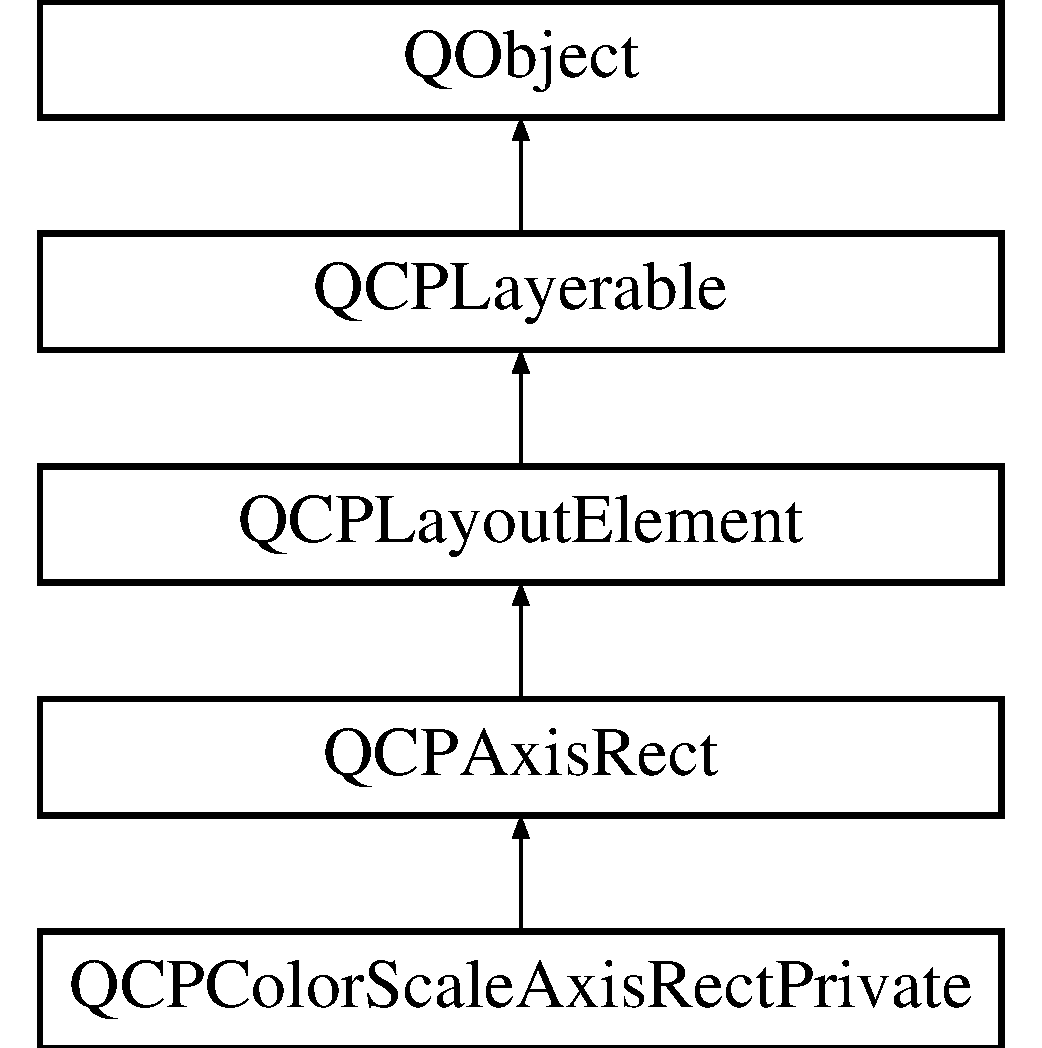
\includegraphics[height=5.000000cm]{class_q_c_p_axis_rect}
\end{center}
\end{figure}
\subsection*{Public Member Functions}
\begin{DoxyCompactItemize}
\item 
\hyperlink{class_q_c_p_axis_rect_a60b31dece805462c1b82eea2e69ba042}{Q\+C\+P\+Axis\+Rect} (\hyperlink{class_q_custom_plot}{Q\+Custom\+Plot} $\ast$parent\+Plot, bool setup\+Default\+Axes=true)
\item 
\hypertarget{class_q_c_p_axis_rect_a572deec9c9a4d5987d5c5f78521991e6}{}\label{class_q_c_p_axis_rect_a572deec9c9a4d5987d5c5f78521991e6} 
Q\+Pixmap {\bfseries background} () const
\item 
\hypertarget{class_q_c_p_axis_rect_a059ede9a5fdcafb5cef280cd65fe4f3a}{}\label{class_q_c_p_axis_rect_a059ede9a5fdcafb5cef280cd65fe4f3a} 
bool {\bfseries background\+Scaled} () const
\item 
\hypertarget{class_q_c_p_axis_rect_a06b98faf54b5491bff780294e423d3ff}{}\label{class_q_c_p_axis_rect_a06b98faf54b5491bff780294e423d3ff} 
Qt\+::\+Aspect\+Ratio\+Mode {\bfseries background\+Scaled\+Mode} () const
\item 
\hypertarget{class_q_c_p_axis_rect_aa3a84c768ad6edd08fd4c5dec176828f}{}\label{class_q_c_p_axis_rect_aa3a84c768ad6edd08fd4c5dec176828f} 
Qt\+::\+Orientations {\bfseries range\+Drag} () const
\item 
\hypertarget{class_q_c_p_axis_rect_aa0d8414ef040523f8b2d55f0c0bddbee}{}\label{class_q_c_p_axis_rect_aa0d8414ef040523f8b2d55f0c0bddbee} 
Qt\+::\+Orientations {\bfseries range\+Zoom} () const
\item 
\hyperlink{class_q_c_p_axis}{Q\+C\+P\+Axis} $\ast$ \hyperlink{class_q_c_p_axis_rect_a6d7c22cfc54fac7a3d6ef80b133a8574}{range\+Drag\+Axis} (Qt\+::\+Orientation orientation)
\item 
\hyperlink{class_q_c_p_axis}{Q\+C\+P\+Axis} $\ast$ \hyperlink{class_q_c_p_axis_rect_a679c63f2b8daccfe6ec5110dce3dd3b6}{range\+Zoom\+Axis} (Qt\+::\+Orientation orientation)
\item 
double \hyperlink{class_q_c_p_axis_rect_ae4e6c4d143aacc88d2d3c56f117c2fe1}{range\+Zoom\+Factor} (Qt\+::\+Orientation orientation)
\item 
void \hyperlink{class_q_c_p_axis_rect_af615ab5e52b8e0a9a0eff415b6559db5}{set\+Background} (const Q\+Pixmap \&pm)
\item 
void \hyperlink{class_q_c_p_axis_rect_ac48a2d5d9b7732e73b86605c69c5e4c1}{set\+Background} (const Q\+Pixmap \&pm, bool scaled, Qt\+::\+Aspect\+Ratio\+Mode mode=Qt\+::\+Keep\+Aspect\+Ratio\+By\+Expanding)
\item 
void \hyperlink{class_q_c_p_axis_rect_a22a22b8668735438dc06f9a55fe46b33}{set\+Background} (const Q\+Brush \&brush)
\item 
void \hyperlink{class_q_c_p_axis_rect_ae6d36c3e0e968ffb991170a018e7b503}{set\+Background\+Scaled} (bool scaled)
\item 
void \hyperlink{class_q_c_p_axis_rect_a5ef77ea829c9de7ba248e473f48f7305}{set\+Background\+Scaled\+Mode} (Qt\+::\+Aspect\+Ratio\+Mode mode)
\item 
void \hyperlink{class_q_c_p_axis_rect_ae6aef2f7211ba6097c925dcd26008418}{set\+Range\+Drag} (Qt\+::\+Orientations orientations)
\item 
void \hyperlink{class_q_c_p_axis_rect_a7960a9d222f1c31d558b064b60f86a31}{set\+Range\+Zoom} (Qt\+::\+Orientations orientations)
\item 
void \hyperlink{class_q_c_p_axis_rect_a648cce336bd99daac4a5ca3e5743775d}{set\+Range\+Drag\+Axes} (\hyperlink{class_q_c_p_axis}{Q\+C\+P\+Axis} $\ast$horizontal, \hyperlink{class_q_c_p_axis}{Q\+C\+P\+Axis} $\ast$vertical)
\item 
void \hyperlink{class_q_c_p_axis_rect_a9442cca2aa358405f39a64d51eca13d2}{set\+Range\+Zoom\+Axes} (\hyperlink{class_q_c_p_axis}{Q\+C\+P\+Axis} $\ast$horizontal, \hyperlink{class_q_c_p_axis}{Q\+C\+P\+Axis} $\ast$vertical)
\item 
void \hyperlink{class_q_c_p_axis_rect_a895d7ac745ea614e04056244b3c138ac}{set\+Range\+Zoom\+Factor} (double horizontal\+Factor, double vertical\+Factor)
\item 
void \hyperlink{class_q_c_p_axis_rect_ae83d187b03fc6fa4f00765ad50cd3fc3}{set\+Range\+Zoom\+Factor} (double factor)
\item 
int \hyperlink{class_q_c_p_axis_rect_a85b321acec0f694d8b5fdeafdbff3133}{axis\+Count} (\hyperlink{class_q_c_p_axis_ae2bcc1728b382f10f064612b368bc18a}{Q\+C\+P\+Axis\+::\+Axis\+Type} type) const
\item 
\hyperlink{class_q_c_p_axis}{Q\+C\+P\+Axis} $\ast$ \hyperlink{class_q_c_p_axis_rect_a583ae4f6d78b601b732183f6cabecbe1}{axis} (\hyperlink{class_q_c_p_axis_ae2bcc1728b382f10f064612b368bc18a}{Q\+C\+P\+Axis\+::\+Axis\+Type} type, int index=0) const
\item 
Q\+List$<$ \hyperlink{class_q_c_p_axis}{Q\+C\+P\+Axis} $\ast$ $>$ \hyperlink{class_q_c_p_axis_rect_a8db4722cb93e9c4a6f0d91150c200867}{axes} (Q\+C\+P\+Axis\+::\+Axis\+Types types) const
\item 
Q\+List$<$ \hyperlink{class_q_c_p_axis}{Q\+C\+P\+Axis} $\ast$ $>$ \hyperlink{class_q_c_p_axis_rect_a11657b8faebe9677180860e8057ede26}{axes} () const
\item 
\hyperlink{class_q_c_p_axis}{Q\+C\+P\+Axis} $\ast$ \hyperlink{class_q_c_p_axis_rect_a2dc336092ccc57d44a46194c8a23e4f4}{add\+Axis} (\hyperlink{class_q_c_p_axis_ae2bcc1728b382f10f064612b368bc18a}{Q\+C\+P\+Axis\+::\+Axis\+Type} type, \hyperlink{class_q_c_p_axis}{Q\+C\+P\+Axis} $\ast$\hyperlink{class_q_c_p_axis_rect_a583ae4f6d78b601b732183f6cabecbe1}{axis}=0)
\item 
Q\+List$<$ \hyperlink{class_q_c_p_axis}{Q\+C\+P\+Axis} $\ast$ $>$ \hyperlink{class_q_c_p_axis_rect_a792e1f3d9cb1591fca135bb0de9b81fc}{add\+Axes} (Q\+C\+P\+Axis\+::\+Axis\+Types types)
\item 
bool \hyperlink{class_q_c_p_axis_rect_a03c39cd9704f0d36fb6cf980cdddcbaa}{remove\+Axis} (\hyperlink{class_q_c_p_axis}{Q\+C\+P\+Axis} $\ast$\hyperlink{class_q_c_p_axis_rect_a583ae4f6d78b601b732183f6cabecbe1}{axis})
\item 
\hyperlink{class_q_c_p_layout_inset}{Q\+C\+P\+Layout\+Inset} $\ast$ \hyperlink{class_q_c_p_axis_rect_a949f803466619924c7018df4b511ae10}{inset\+Layout} () const
\item 
void \hyperlink{class_q_c_p_axis_rect_a5fa906175447b14206954f77fc7f1ef4}{setup\+Full\+Axes\+Box} (bool connect\+Ranges=false)
\item 
Q\+List$<$ \hyperlink{class_q_c_p_abstract_plottable}{Q\+C\+P\+Abstract\+Plottable} $\ast$ $>$ \hyperlink{class_q_c_p_axis_rect_a587d073a97b27bc7293fab4b2774ad59}{plottables} () const
\item 
Q\+List$<$ \hyperlink{class_q_c_p_graph}{Q\+C\+P\+Graph} $\ast$ $>$ \hyperlink{class_q_c_p_axis_rect_a2d9ded3eca97be1fcb5867949391bb88}{graphs} () const
\item 
Q\+List$<$ \hyperlink{class_q_c_p_abstract_item}{Q\+C\+P\+Abstract\+Item} $\ast$ $>$ \hyperlink{class_q_c_p_axis_rect_a03c113a2175448300ee8f944e24776ba}{items} () const
\item 
int \hyperlink{class_q_c_p_axis_rect_afb4a3de02046b20b9310bdb8fca781c3}{left} () const
\item 
int \hyperlink{class_q_c_p_axis_rect_a3f819d4a1b2193723d1fdafc573eea10}{right} () const
\item 
int \hyperlink{class_q_c_p_axis_rect_a45dbad181cbb9f09d068dbb76c817c95}{top} () const
\item 
int \hyperlink{class_q_c_p_axis_rect_acefdf1abaa8a8ab681e906cc2be9581e}{bottom} () const
\item 
int \hyperlink{class_q_c_p_axis_rect_a204645398a4f9d0b0189385c7c2cfb91}{width} () const
\item 
int \hyperlink{class_q_c_p_axis_rect_acc4377809e79d9a089ab790f39429b0d}{height} () const
\item 
Q\+Size \hyperlink{class_q_c_p_axis_rect_a7a8289346eb612f422c704f8b75cf479}{size} () const
\item 
Q\+Point \hyperlink{class_q_c_p_axis_rect_a5a847b3ddeca3abec38d3838fefb0dbd}{top\+Left} () const
\item 
Q\+Point \hyperlink{class_q_c_p_axis_rect_a7aa221967549ba71b98c465bf8234758}{top\+Right} () const
\item 
Q\+Point \hyperlink{class_q_c_p_axis_rect_ab15d4311d6535ccd7af504dc0e2b98c6}{bottom\+Left} () const
\item 
Q\+Point \hyperlink{class_q_c_p_axis_rect_a36dac884ec8fa3a3a2f3842ca7b7d32d}{bottom\+Right} () const
\item 
Q\+Point \hyperlink{class_q_c_p_axis_rect_ade3aef874bafcec6dd16174fba44c0b1}{center} () const
\item 
virtual void \hyperlink{class_q_c_p_axis_rect_a255080a017df9083a60a321ef2ba9ed8}{update} (\hyperlink{class_q_c_p_layout_element_a0d83360e05735735aaf6d7983c56374d}{Update\+Phase} phase)
\item 
virtual Q\+List$<$ \hyperlink{class_q_c_p_layout_element}{Q\+C\+P\+Layout\+Element} $\ast$ $>$ \hyperlink{class_q_c_p_axis_rect_a40c0b3b17eb317ff4d393b7cb9b082a2}{elements} (bool recursive) const
\end{DoxyCompactItemize}
\subsection*{Protected Member Functions}
\begin{DoxyCompactItemize}
\item 
\hypertarget{class_q_c_p_axis_rect_aa954ebda9ddbc74146ab9b47abad277b}{}\label{class_q_c_p_axis_rect_aa954ebda9ddbc74146ab9b47abad277b} 
virtual void {\bfseries apply\+Default\+Antialiasing\+Hint} (\hyperlink{class_q_c_p_painter}{Q\+C\+P\+Painter} $\ast$painter) const
\item 
\hypertarget{class_q_c_p_axis_rect_afb1bbbbda8345cd2710d92ee48440b53}{}\label{class_q_c_p_axis_rect_afb1bbbbda8345cd2710d92ee48440b53} 
virtual void {\bfseries draw} (\hyperlink{class_q_c_p_painter}{Q\+C\+P\+Painter} $\ast$painter)
\item 
\hypertarget{class_q_c_p_axis_rect_ae79f18302e6507586aa8c032a5f9ed1c}{}\label{class_q_c_p_axis_rect_ae79f18302e6507586aa8c032a5f9ed1c} 
virtual int {\bfseries calculate\+Auto\+Margin} (\hyperlink{namespace_q_c_p_a7e487e3e2ccb62ab7771065bab7cae54}{Q\+C\+P\+::\+Margin\+Side} side)
\item 
virtual void \hyperlink{class_q_c_p_axis_rect_a77501dbeccdac7256f7979b05077c04e}{mouse\+Press\+Event} (Q\+Mouse\+Event $\ast$event)
\item 
virtual void \hyperlink{class_q_c_p_axis_rect_a4baf3d5dd69166788f6ceda0ea182c6e}{mouse\+Move\+Event} (Q\+Mouse\+Event $\ast$event)
\item 
virtual void \hyperlink{class_q_c_p_axis_rect_adf6c99780cea55ab39459a6eaad3a94a}{mouse\+Release\+Event} (Q\+Mouse\+Event $\ast$event)
\item 
virtual void \hyperlink{class_q_c_p_axis_rect_a5acf41fc30aa68ea263246ecfad85c31}{wheel\+Event} (Q\+Wheel\+Event $\ast$event)
\item 
\hypertarget{class_q_c_p_axis_rect_ab49d338d1ce74b476fcead5b32cf06dc}{}\label{class_q_c_p_axis_rect_ab49d338d1ce74b476fcead5b32cf06dc} 
void {\bfseries draw\+Background} (\hyperlink{class_q_c_p_painter}{Q\+C\+P\+Painter} $\ast$painter)
\item 
\hypertarget{class_q_c_p_axis_rect_a6024ccdc74f5dc0e8a0fe482e5b28a20}{}\label{class_q_c_p_axis_rect_a6024ccdc74f5dc0e8a0fe482e5b28a20} 
void {\bfseries update\+Axes\+Offset} (\hyperlink{class_q_c_p_axis_ae2bcc1728b382f10f064612b368bc18a}{Q\+C\+P\+Axis\+::\+Axis\+Type} type)
\end{DoxyCompactItemize}
\subsection*{Protected Attributes}
\begin{DoxyCompactItemize}
\item 
\hypertarget{class_q_c_p_axis_rect_a5748e1a37f63c428e38b0a7724b46259}{}\label{class_q_c_p_axis_rect_a5748e1a37f63c428e38b0a7724b46259} 
Q\+Brush {\bfseries m\+Background\+Brush}
\item 
\hypertarget{class_q_c_p_axis_rect_a38fb1a15f43228a0c124553649303722}{}\label{class_q_c_p_axis_rect_a38fb1a15f43228a0c124553649303722} 
Q\+Pixmap {\bfseries m\+Background\+Pixmap}
\item 
\hypertarget{class_q_c_p_axis_rect_aa74b9415598d59b49290e41e42d7ee27}{}\label{class_q_c_p_axis_rect_aa74b9415598d59b49290e41e42d7ee27} 
Q\+Pixmap {\bfseries m\+Scaled\+Background\+Pixmap}
\item 
\hypertarget{class_q_c_p_axis_rect_a5ad835f0fae5d7cc5ada9e063641dbf1}{}\label{class_q_c_p_axis_rect_a5ad835f0fae5d7cc5ada9e063641dbf1} 
bool {\bfseries m\+Background\+Scaled}
\item 
\hypertarget{class_q_c_p_axis_rect_a859fd368e794663e346b4f53f35078e9}{}\label{class_q_c_p_axis_rect_a859fd368e794663e346b4f53f35078e9} 
Qt\+::\+Aspect\+Ratio\+Mode {\bfseries m\+Background\+Scaled\+Mode}
\item 
\hypertarget{class_q_c_p_axis_rect_a255240399e0fd24baad80cbbe46f698a}{}\label{class_q_c_p_axis_rect_a255240399e0fd24baad80cbbe46f698a} 
\hyperlink{class_q_c_p_layout_inset}{Q\+C\+P\+Layout\+Inset} $\ast$ {\bfseries m\+Inset\+Layout}
\item 
\hypertarget{class_q_c_p_axis_rect_aa9f107f66ca3469ad50ee6cea7c9e237}{}\label{class_q_c_p_axis_rect_aa9f107f66ca3469ad50ee6cea7c9e237} 
Qt\+::\+Orientations {\bfseries m\+Range\+Drag}
\item 
\hypertarget{class_q_c_p_axis_rect_a215eff671d48df2edccc36e7f976f28c}{}\label{class_q_c_p_axis_rect_a215eff671d48df2edccc36e7f976f28c} 
Qt\+::\+Orientations {\bfseries m\+Range\+Zoom}
\item 
\hypertarget{class_q_c_p_axis_rect_aeaaa38c6d2030dd5f84461e2596e41e3}{}\label{class_q_c_p_axis_rect_aeaaa38c6d2030dd5f84461e2596e41e3} 
Q\+Pointer$<$ \hyperlink{class_q_c_p_axis}{Q\+C\+P\+Axis} $>$ {\bfseries m\+Range\+Drag\+Horz\+Axis}
\item 
\hypertarget{class_q_c_p_axis_rect_a3e41dffec18987366f2a8ffd80689c12}{}\label{class_q_c_p_axis_rect_a3e41dffec18987366f2a8ffd80689c12} 
Q\+Pointer$<$ \hyperlink{class_q_c_p_axis}{Q\+C\+P\+Axis} $>$ {\bfseries m\+Range\+Drag\+Vert\+Axis}
\item 
\hypertarget{class_q_c_p_axis_rect_ae22f882bab20518559f3fbb84243d0ab}{}\label{class_q_c_p_axis_rect_ae22f882bab20518559f3fbb84243d0ab} 
Q\+Pointer$<$ \hyperlink{class_q_c_p_axis}{Q\+C\+P\+Axis} $>$ {\bfseries m\+Range\+Zoom\+Horz\+Axis}
\item 
\hypertarget{class_q_c_p_axis_rect_a8b9acd16a203a9692bd35a9465f54bc1}{}\label{class_q_c_p_axis_rect_a8b9acd16a203a9692bd35a9465f54bc1} 
Q\+Pointer$<$ \hyperlink{class_q_c_p_axis}{Q\+C\+P\+Axis} $>$ {\bfseries m\+Range\+Zoom\+Vert\+Axis}
\item 
\hypertarget{class_q_c_p_axis_rect_ad08d0250ed7b99de387d0ea6c7fd4dc1}{}\label{class_q_c_p_axis_rect_ad08d0250ed7b99de387d0ea6c7fd4dc1} 
double {\bfseries m\+Range\+Zoom\+Factor\+Horz}
\item 
\hypertarget{class_q_c_p_axis_rect_a32f063629581d5bf82b12769940b34ad}{}\label{class_q_c_p_axis_rect_a32f063629581d5bf82b12769940b34ad} 
double {\bfseries m\+Range\+Zoom\+Factor\+Vert}
\item 
\hypertarget{class_q_c_p_axis_rect_a41936cf473ec638bec382f5a40cdb1f3}{}\label{class_q_c_p_axis_rect_a41936cf473ec638bec382f5a40cdb1f3} 
\hyperlink{class_q_c_p_range}{Q\+C\+P\+Range} {\bfseries m\+Drag\+Start\+Horz\+Range}
\item 
\hypertarget{class_q_c_p_axis_rect_a1a5ae4c74b8bd46baf91bf4e4f4165f0}{}\label{class_q_c_p_axis_rect_a1a5ae4c74b8bd46baf91bf4e4f4165f0} 
\hyperlink{class_q_c_p_range}{Q\+C\+P\+Range} {\bfseries m\+Drag\+Start\+Vert\+Range}
\item 
\hypertarget{class_q_c_p_axis_rect_aa4a24f76360cfebe1bcf17a77fa7521b}{}\label{class_q_c_p_axis_rect_aa4a24f76360cfebe1bcf17a77fa7521b} 
Q\+C\+P\+::\+Antialiased\+Elements {\bfseries m\+A\+A\+Drag\+Backup}
\item 
\hypertarget{class_q_c_p_axis_rect_a6fcb12e052e276d57efbb128be31d6f5}{}\label{class_q_c_p_axis_rect_a6fcb12e052e276d57efbb128be31d6f5} 
Q\+C\+P\+::\+Antialiased\+Elements {\bfseries m\+Not\+A\+A\+Drag\+Backup}
\item 
\hypertarget{class_q_c_p_axis_rect_a032896b28f83a58010d8d533b78c49df}{}\label{class_q_c_p_axis_rect_a032896b28f83a58010d8d533b78c49df} 
Q\+Point {\bfseries m\+Drag\+Start}
\item 
\hypertarget{class_q_c_p_axis_rect_ab49a6698194cf0e9e38a1d734c0888a8}{}\label{class_q_c_p_axis_rect_ab49a6698194cf0e9e38a1d734c0888a8} 
bool {\bfseries m\+Dragging}
\item 
\hypertarget{class_q_c_p_axis_rect_afe7a24d2a2bea98fc552fa826350ba81}{}\label{class_q_c_p_axis_rect_afe7a24d2a2bea98fc552fa826350ba81} 
Q\+Hash$<$ \hyperlink{class_q_c_p_axis_ae2bcc1728b382f10f064612b368bc18a}{Q\+C\+P\+Axis\+::\+Axis\+Type}, Q\+List$<$ \hyperlink{class_q_c_p_axis}{Q\+C\+P\+Axis} $\ast$ $>$ $>$ {\bfseries m\+Axes}
\end{DoxyCompactItemize}
\subsection*{Friends}
\begin{DoxyCompactItemize}
\item 
\hypertarget{class_q_c_p_axis_rect_a1cdf9df76adcfae45261690aa0ca2198}{}\label{class_q_c_p_axis_rect_a1cdf9df76adcfae45261690aa0ca2198} 
class {\bfseries Q\+Custom\+Plot}
\end{DoxyCompactItemize}
\subsection*{Additional Inherited Members}


\subsection{Detailed Description}
Holds multiple axes and arranges them in a rectangular shape. 

This class represents an axis rect, a rectangular area that is bounded on all sides with an arbitrary number of axes.

Initially \hyperlink{class_q_custom_plot}{Q\+Custom\+Plot} has one axis rect, accessible via \hyperlink{class_q_custom_plot_ae5eefcb5f6ca26689b1fd4f6e25b42f9}{Q\+Custom\+Plot\+::axis\+Rect()}. However, the layout system allows to have multiple axis rects, e.\+g. arranged in a grid layout (\hyperlink{class_q_custom_plot_af1a1f1f571237deb7c2bd34a5e9f018f}{Q\+Custom\+Plot\+::plot\+Layout}).

By default, \hyperlink{class_q_c_p_axis_rect}{Q\+C\+P\+Axis\+Rect} comes with four axes, at bottom, top, left and right. They can be accessed via \hyperlink{class_q_c_p_axis_rect_a583ae4f6d78b601b732183f6cabecbe1}{axis} by providing the respective axis type (\hyperlink{class_q_c_p_axis_ae2bcc1728b382f10f064612b368bc18a}{Q\+C\+P\+Axis\+::\+Axis\+Type}) and index. If you need all axes in the axis rect, use \hyperlink{class_q_c_p_axis_rect_a8db4722cb93e9c4a6f0d91150c200867}{axes}. The top and right axes are set to be invisible initially (\hyperlink{class_q_c_p_layerable_a3bed99ddc396b48ce3ebfdc0418744f8}{Q\+C\+P\+Axis\+::set\+Visible}). To add more axes to a side, use \hyperlink{class_q_c_p_axis_rect_a2dc336092ccc57d44a46194c8a23e4f4}{add\+Axis} or \hyperlink{class_q_c_p_axis_rect_a792e1f3d9cb1591fca135bb0de9b81fc}{add\+Axes}. To remove an axis, use \hyperlink{class_q_c_p_axis_rect_a03c39cd9704f0d36fb6cf980cdddcbaa}{remove\+Axis}.

The axis rect layerable itself only draws a background pixmap or color, if specified (\hyperlink{class_q_c_p_axis_rect_af615ab5e52b8e0a9a0eff415b6559db5}{set\+Background}). It is placed on the \char`\"{}background\char`\"{} layer initially (see \hyperlink{class_q_c_p_layer}{Q\+C\+P\+Layer} for an explanation of the \hyperlink{class_q_custom_plot}{Q\+Custom\+Plot} layer system). The axes that are held by the axis rect can be placed on other layers, independently of the axis rect.

Every axis rect has a child layout of type \hyperlink{class_q_c_p_layout_inset}{Q\+C\+P\+Layout\+Inset}. It is accessible via \hyperlink{class_q_c_p_axis_rect_a949f803466619924c7018df4b511ae10}{inset\+Layout} and can be used to have other layout elements (or even other layouts with multiple elements) hovering inside the axis rect.

If an axis rect is clicked and dragged, it processes this by moving certain axis ranges. The behaviour can be controlled with \hyperlink{class_q_c_p_axis_rect_ae6aef2f7211ba6097c925dcd26008418}{set\+Range\+Drag} and \hyperlink{class_q_c_p_axis_rect_a648cce336bd99daac4a5ca3e5743775d}{set\+Range\+Drag\+Axes}. If the mouse wheel is scrolled while the cursor is on the axis rect, certain axes are scaled. This is controllable via \hyperlink{class_q_c_p_axis_rect_a7960a9d222f1c31d558b064b60f86a31}{set\+Range\+Zoom}, \hyperlink{class_q_c_p_axis_rect_a9442cca2aa358405f39a64d51eca13d2}{set\+Range\+Zoom\+Axes} and \hyperlink{class_q_c_p_axis_rect_a895d7ac745ea614e04056244b3c138ac}{set\+Range\+Zoom\+Factor}. These interactions are only enabled if \hyperlink{class_q_custom_plot_a5ee1e2f6ae27419deca53e75907c27e5}{Q\+Custom\+Plot\+::set\+Interactions} contains \hyperlink{namespace_q_c_p_a2ad6bb6281c7c2d593d4277b44c2b037a2c4432b9aceafb94000be8d1b589ef18}{Q\+C\+P\+::i\+Range\+Drag} and \hyperlink{namespace_q_c_p_a2ad6bb6281c7c2d593d4277b44c2b037abee1e94353525a636aeaf0ba32b72e14}{Q\+C\+P\+::i\+Range\+Zoom}.

 \begin{center}Overview of the spacings and paddings that define the geometry of an axis. The dashed line on the far left indicates the viewport/widget border.\end{center}  

\subsection{Constructor \& Destructor Documentation}
\hypertarget{class_q_c_p_axis_rect_a60b31dece805462c1b82eea2e69ba042}{}\label{class_q_c_p_axis_rect_a60b31dece805462c1b82eea2e69ba042} 
\index{Q\+C\+P\+Axis\+Rect@{Q\+C\+P\+Axis\+Rect}!Q\+C\+P\+Axis\+Rect@{Q\+C\+P\+Axis\+Rect}}
\index{Q\+C\+P\+Axis\+Rect@{Q\+C\+P\+Axis\+Rect}!Q\+C\+P\+Axis\+Rect@{Q\+C\+P\+Axis\+Rect}}
\subsubsection{\texorpdfstring{Q\+C\+P\+Axis\+Rect()}{QCPAxisRect()}}
{\footnotesize\ttfamily Q\+C\+P\+Axis\+Rect\+::\+Q\+C\+P\+Axis\+Rect (\begin{DoxyParamCaption}\item[{\hyperlink{class_q_custom_plot}{Q\+Custom\+Plot} $\ast$}]{parent\+Plot,  }\item[{bool}]{setup\+Default\+Axes = {\ttfamily true} }\end{DoxyParamCaption})\hspace{0.3cm}{\ttfamily [explicit]}}

Creates a \hyperlink{class_q_c_p_axis_rect}{Q\+C\+P\+Axis\+Rect} instance and sets default values. An axis is added for each of the four sides, the top and right axes are set invisible initially. 

\subsection{Member Function Documentation}
\hypertarget{class_q_c_p_axis_rect_a792e1f3d9cb1591fca135bb0de9b81fc}{}\label{class_q_c_p_axis_rect_a792e1f3d9cb1591fca135bb0de9b81fc} 
\index{Q\+C\+P\+Axis\+Rect@{Q\+C\+P\+Axis\+Rect}!add\+Axes@{add\+Axes}}
\index{add\+Axes@{add\+Axes}!Q\+C\+P\+Axis\+Rect@{Q\+C\+P\+Axis\+Rect}}
\subsubsection{\texorpdfstring{add\+Axes()}{addAxes()}}
{\footnotesize\ttfamily Q\+List$<$ \hyperlink{class_q_c_p_axis}{Q\+C\+P\+Axis} $\ast$ $>$ Q\+C\+P\+Axis\+Rect\+::add\+Axes (\begin{DoxyParamCaption}\item[{Q\+C\+P\+Axis\+::\+Axis\+Types}]{types }\end{DoxyParamCaption})}

Adds a new axis with \hyperlink{class_q_c_p_axis_rect_a2dc336092ccc57d44a46194c8a23e4f4}{add\+Axis} to each axis rect side specified in {\itshape types}. This may be an {\ttfamily or}-\/combination of \hyperlink{class_q_c_p_axis_ae2bcc1728b382f10f064612b368bc18a}{Q\+C\+P\+Axis\+::\+Axis\+Type}, so axes can be added to multiple sides at once.

Returns a list of the added axes.

\begin{DoxySeeAlso}{See also}
\hyperlink{class_q_c_p_axis_rect_a2dc336092ccc57d44a46194c8a23e4f4}{add\+Axis}, \hyperlink{class_q_c_p_axis_rect_a5fa906175447b14206954f77fc7f1ef4}{setup\+Full\+Axes\+Box} 
\end{DoxySeeAlso}
\hypertarget{class_q_c_p_axis_rect_a2dc336092ccc57d44a46194c8a23e4f4}{}\label{class_q_c_p_axis_rect_a2dc336092ccc57d44a46194c8a23e4f4} 
\index{Q\+C\+P\+Axis\+Rect@{Q\+C\+P\+Axis\+Rect}!add\+Axis@{add\+Axis}}
\index{add\+Axis@{add\+Axis}!Q\+C\+P\+Axis\+Rect@{Q\+C\+P\+Axis\+Rect}}
\subsubsection{\texorpdfstring{add\+Axis()}{addAxis()}}
{\footnotesize\ttfamily \hyperlink{class_q_c_p_axis}{Q\+C\+P\+Axis} $\ast$ Q\+C\+P\+Axis\+Rect\+::add\+Axis (\begin{DoxyParamCaption}\item[{\hyperlink{class_q_c_p_axis_ae2bcc1728b382f10f064612b368bc18a}{Q\+C\+P\+Axis\+::\+Axis\+Type}}]{type,  }\item[{\hyperlink{class_q_c_p_axis}{Q\+C\+P\+Axis} $\ast$}]{axis = {\ttfamily 0} }\end{DoxyParamCaption})}

Adds a new axis to the axis rect side specified with {\itshape type}, and returns it. If {\itshape axis} is 0, a new \hyperlink{class_q_c_p_axis}{Q\+C\+P\+Axis} instance is created internally.

You may inject \hyperlink{class_q_c_p_axis}{Q\+C\+P\+Axis} instances (or sublasses of \hyperlink{class_q_c_p_axis}{Q\+C\+P\+Axis}) by setting {\itshape axis} to an axis that was previously created outside \hyperlink{class_q_custom_plot}{Q\+Custom\+Plot}. It is important to note that \hyperlink{class_q_custom_plot}{Q\+Custom\+Plot} takes ownership of the axis, so you may not delete it afterwards. Further, the {\itshape axis} must have been created with this axis rect as parent and with the same axis type as specified in {\itshape type}. If this is not the case, a debug output is generated, the axis is not added, and the method returns 0.

This method can not be used to move {\itshape axis} between axis rects. The same {\itshape axis} instance must not be added multiple times to the same or different axis rects.

If an axis rect side already contains one or more axes, the lower and upper endings of the new axis (\hyperlink{class_q_c_p_axis_a08af1c72db9ae4dc8cb8a973d44405ab}{Q\+C\+P\+Axis\+::set\+Lower\+Ending}, \hyperlink{class_q_c_p_axis_a69119b892fc306f651763596685aa377}{Q\+C\+P\+Axis\+::set\+Upper\+Ending}) are set to \hyperlink{class_q_c_p_line_ending_a5ef16e6876b4b74959c7261d8d4c2cd5a126c390f0c359fcd8df1fc5e38d26d5b}{Q\+C\+P\+Line\+Ending\+::es\+Half\+Bar}.

\begin{DoxySeeAlso}{See also}
\hyperlink{class_q_c_p_axis_rect_a792e1f3d9cb1591fca135bb0de9b81fc}{add\+Axes}, \hyperlink{class_q_c_p_axis_rect_a5fa906175447b14206954f77fc7f1ef4}{setup\+Full\+Axes\+Box} 
\end{DoxySeeAlso}
\hypertarget{class_q_c_p_axis_rect_a8db4722cb93e9c4a6f0d91150c200867}{}\label{class_q_c_p_axis_rect_a8db4722cb93e9c4a6f0d91150c200867} 
\index{Q\+C\+P\+Axis\+Rect@{Q\+C\+P\+Axis\+Rect}!axes@{axes}}
\index{axes@{axes}!Q\+C\+P\+Axis\+Rect@{Q\+C\+P\+Axis\+Rect}}
\subsubsection{\texorpdfstring{axes()}{axes()}\hspace{0.1cm}{\footnotesize\ttfamily [1/2]}}
{\footnotesize\ttfamily Q\+List$<$ \hyperlink{class_q_c_p_axis}{Q\+C\+P\+Axis} $\ast$ $>$ Q\+C\+P\+Axis\+Rect\+::axes (\begin{DoxyParamCaption}\item[{Q\+C\+P\+Axis\+::\+Axis\+Types}]{types }\end{DoxyParamCaption}) const}

Returns all axes on the axis rect sides specified with {\itshape types}.

{\itshape types} may be a single \hyperlink{class_q_c_p_axis_ae2bcc1728b382f10f064612b368bc18a}{Q\+C\+P\+Axis\+::\+Axis\+Type} or an {\ttfamily or}-\/combination, to get the axes of multiple sides.

\begin{DoxySeeAlso}{See also}
\hyperlink{class_q_c_p_axis_rect_a583ae4f6d78b601b732183f6cabecbe1}{axis} 
\end{DoxySeeAlso}
\hypertarget{class_q_c_p_axis_rect_a11657b8faebe9677180860e8057ede26}{}\label{class_q_c_p_axis_rect_a11657b8faebe9677180860e8057ede26} 
\index{Q\+C\+P\+Axis\+Rect@{Q\+C\+P\+Axis\+Rect}!axes@{axes}}
\index{axes@{axes}!Q\+C\+P\+Axis\+Rect@{Q\+C\+P\+Axis\+Rect}}
\subsubsection{\texorpdfstring{axes()}{axes()}\hspace{0.1cm}{\footnotesize\ttfamily [2/2]}}
{\footnotesize\ttfamily Q\+List$<$ \hyperlink{class_q_c_p_axis}{Q\+C\+P\+Axis} $\ast$ $>$ Q\+C\+P\+Axis\+Rect\+::axes (\begin{DoxyParamCaption}{ }\end{DoxyParamCaption}) const}

This is an overloaded member function, provided for convenience. It differs from the above function only in what argument(s) it accepts.

Returns all axes of this axis rect. \hypertarget{class_q_c_p_axis_rect_a583ae4f6d78b601b732183f6cabecbe1}{}\label{class_q_c_p_axis_rect_a583ae4f6d78b601b732183f6cabecbe1} 
\index{Q\+C\+P\+Axis\+Rect@{Q\+C\+P\+Axis\+Rect}!axis@{axis}}
\index{axis@{axis}!Q\+C\+P\+Axis\+Rect@{Q\+C\+P\+Axis\+Rect}}
\subsubsection{\texorpdfstring{axis()}{axis()}}
{\footnotesize\ttfamily \hyperlink{class_q_c_p_axis}{Q\+C\+P\+Axis} $\ast$ Q\+C\+P\+Axis\+Rect\+::axis (\begin{DoxyParamCaption}\item[{\hyperlink{class_q_c_p_axis_ae2bcc1728b382f10f064612b368bc18a}{Q\+C\+P\+Axis\+::\+Axis\+Type}}]{type,  }\item[{int}]{index = {\ttfamily 0} }\end{DoxyParamCaption}) const}

Returns the axis with the given {\itshape index} on the axis rect side specified with {\itshape type}.

\begin{DoxySeeAlso}{See also}
\hyperlink{class_q_c_p_axis_rect_a85b321acec0f694d8b5fdeafdbff3133}{axis\+Count}, \hyperlink{class_q_c_p_axis_rect_a8db4722cb93e9c4a6f0d91150c200867}{axes} 
\end{DoxySeeAlso}
\hypertarget{class_q_c_p_axis_rect_a85b321acec0f694d8b5fdeafdbff3133}{}\label{class_q_c_p_axis_rect_a85b321acec0f694d8b5fdeafdbff3133} 
\index{Q\+C\+P\+Axis\+Rect@{Q\+C\+P\+Axis\+Rect}!axis\+Count@{axis\+Count}}
\index{axis\+Count@{axis\+Count}!Q\+C\+P\+Axis\+Rect@{Q\+C\+P\+Axis\+Rect}}
\subsubsection{\texorpdfstring{axis\+Count()}{axisCount()}}
{\footnotesize\ttfamily int Q\+C\+P\+Axis\+Rect\+::axis\+Count (\begin{DoxyParamCaption}\item[{\hyperlink{class_q_c_p_axis_ae2bcc1728b382f10f064612b368bc18a}{Q\+C\+P\+Axis\+::\+Axis\+Type}}]{type }\end{DoxyParamCaption}) const}

Returns the number of axes on the axis rect side specified with {\itshape type}.

\begin{DoxySeeAlso}{See also}
\hyperlink{class_q_c_p_axis_rect_a583ae4f6d78b601b732183f6cabecbe1}{axis} 
\end{DoxySeeAlso}
\hypertarget{class_q_c_p_axis_rect_acefdf1abaa8a8ab681e906cc2be9581e}{}\label{class_q_c_p_axis_rect_acefdf1abaa8a8ab681e906cc2be9581e} 
\index{Q\+C\+P\+Axis\+Rect@{Q\+C\+P\+Axis\+Rect}!bottom@{bottom}}
\index{bottom@{bottom}!Q\+C\+P\+Axis\+Rect@{Q\+C\+P\+Axis\+Rect}}
\subsubsection{\texorpdfstring{bottom()}{bottom()}}
{\footnotesize\ttfamily int Q\+C\+P\+Axis\+Rect\+::bottom (\begin{DoxyParamCaption}{ }\end{DoxyParamCaption}) const\hspace{0.3cm}{\ttfamily [inline]}}

Returns the pixel position of the bottom border of this axis rect. Margins are not taken into account here, so the returned value is with respect to the inner \hyperlink{class_q_c_p_layout_element_a208effccfe2cca4a0eaf9393e60f2dd4}{rect}. \hypertarget{class_q_c_p_axis_rect_ab15d4311d6535ccd7af504dc0e2b98c6}{}\label{class_q_c_p_axis_rect_ab15d4311d6535ccd7af504dc0e2b98c6} 
\index{Q\+C\+P\+Axis\+Rect@{Q\+C\+P\+Axis\+Rect}!bottom\+Left@{bottom\+Left}}
\index{bottom\+Left@{bottom\+Left}!Q\+C\+P\+Axis\+Rect@{Q\+C\+P\+Axis\+Rect}}
\subsubsection{\texorpdfstring{bottom\+Left()}{bottomLeft()}}
{\footnotesize\ttfamily Q\+Point Q\+C\+P\+Axis\+Rect\+::bottom\+Left (\begin{DoxyParamCaption}{ }\end{DoxyParamCaption}) const\hspace{0.3cm}{\ttfamily [inline]}}

Returns the bottom left corner of this axis rect in pixels. Margins are not taken into account here, so the returned value is with respect to the inner \hyperlink{class_q_c_p_layout_element_a208effccfe2cca4a0eaf9393e60f2dd4}{rect}. \hypertarget{class_q_c_p_axis_rect_a36dac884ec8fa3a3a2f3842ca7b7d32d}{}\label{class_q_c_p_axis_rect_a36dac884ec8fa3a3a2f3842ca7b7d32d} 
\index{Q\+C\+P\+Axis\+Rect@{Q\+C\+P\+Axis\+Rect}!bottom\+Right@{bottom\+Right}}
\index{bottom\+Right@{bottom\+Right}!Q\+C\+P\+Axis\+Rect@{Q\+C\+P\+Axis\+Rect}}
\subsubsection{\texorpdfstring{bottom\+Right()}{bottomRight()}}
{\footnotesize\ttfamily Q\+Point Q\+C\+P\+Axis\+Rect\+::bottom\+Right (\begin{DoxyParamCaption}{ }\end{DoxyParamCaption}) const\hspace{0.3cm}{\ttfamily [inline]}}

Returns the bottom right corner of this axis rect in pixels. Margins are not taken into account here, so the returned value is with respect to the inner \hyperlink{class_q_c_p_layout_element_a208effccfe2cca4a0eaf9393e60f2dd4}{rect}. \hypertarget{class_q_c_p_axis_rect_ade3aef874bafcec6dd16174fba44c0b1}{}\label{class_q_c_p_axis_rect_ade3aef874bafcec6dd16174fba44c0b1} 
\index{Q\+C\+P\+Axis\+Rect@{Q\+C\+P\+Axis\+Rect}!center@{center}}
\index{center@{center}!Q\+C\+P\+Axis\+Rect@{Q\+C\+P\+Axis\+Rect}}
\subsubsection{\texorpdfstring{center()}{center()}}
{\footnotesize\ttfamily Q\+Point Q\+C\+P\+Axis\+Rect\+::center (\begin{DoxyParamCaption}{ }\end{DoxyParamCaption}) const\hspace{0.3cm}{\ttfamily [inline]}}

Returns the center of this axis rect in pixels. Margins are not taken into account here, so the returned value is with respect to the inner \hyperlink{class_q_c_p_layout_element_a208effccfe2cca4a0eaf9393e60f2dd4}{rect}. \hypertarget{class_q_c_p_axis_rect_a40c0b3b17eb317ff4d393b7cb9b082a2}{}\label{class_q_c_p_axis_rect_a40c0b3b17eb317ff4d393b7cb9b082a2} 
\index{Q\+C\+P\+Axis\+Rect@{Q\+C\+P\+Axis\+Rect}!elements@{elements}}
\index{elements@{elements}!Q\+C\+P\+Axis\+Rect@{Q\+C\+P\+Axis\+Rect}}
\subsubsection{\texorpdfstring{elements()}{elements()}}
{\footnotesize\ttfamily Q\+List$<$ \hyperlink{class_q_c_p_layout_element}{Q\+C\+P\+Layout\+Element} $\ast$ $>$ Q\+C\+P\+Axis\+Rect\+::elements (\begin{DoxyParamCaption}\item[{bool}]{recursive }\end{DoxyParamCaption}) const\hspace{0.3cm}{\ttfamily [virtual]}}

Returns a list of all child elements in this layout element. If {\itshape recursive} is true, all sub-\/child elements are included in the list, too.

\begin{DoxyWarning}{Warning}
There may be entries with value 0 in the returned list. (For example, \hyperlink{class_q_c_p_layout_grid}{Q\+C\+P\+Layout\+Grid} may have empty cells which yield 0 at the respective index.) 
\end{DoxyWarning}


Reimplemented from \hyperlink{class_q_c_p_layout_element_a76dec8cb31e498994a944d7647a43309}{Q\+C\+P\+Layout\+Element}.

\hypertarget{class_q_c_p_axis_rect_a2d9ded3eca97be1fcb5867949391bb88}{}\label{class_q_c_p_axis_rect_a2d9ded3eca97be1fcb5867949391bb88} 
\index{Q\+C\+P\+Axis\+Rect@{Q\+C\+P\+Axis\+Rect}!graphs@{graphs}}
\index{graphs@{graphs}!Q\+C\+P\+Axis\+Rect@{Q\+C\+P\+Axis\+Rect}}
\subsubsection{\texorpdfstring{graphs()}{graphs()}}
{\footnotesize\ttfamily Q\+List$<$ \hyperlink{class_q_c_p_graph}{Q\+C\+P\+Graph} $\ast$ $>$ Q\+C\+P\+Axis\+Rect\+::graphs (\begin{DoxyParamCaption}{ }\end{DoxyParamCaption}) const}

Returns a list of all the graphs that are associated with this axis rect.

A graph is considered associated with an axis rect if its key or value axis (or both) is in this axis rect.

\begin{DoxySeeAlso}{See also}
\hyperlink{class_q_c_p_axis_rect_a587d073a97b27bc7293fab4b2774ad59}{plottables}, \hyperlink{class_q_c_p_axis_rect_a03c113a2175448300ee8f944e24776ba}{items} 
\end{DoxySeeAlso}
\hypertarget{class_q_c_p_axis_rect_acc4377809e79d9a089ab790f39429b0d}{}\label{class_q_c_p_axis_rect_acc4377809e79d9a089ab790f39429b0d} 
\index{Q\+C\+P\+Axis\+Rect@{Q\+C\+P\+Axis\+Rect}!height@{height}}
\index{height@{height}!Q\+C\+P\+Axis\+Rect@{Q\+C\+P\+Axis\+Rect}}
\subsubsection{\texorpdfstring{height()}{height()}}
{\footnotesize\ttfamily int Q\+C\+P\+Axis\+Rect\+::height (\begin{DoxyParamCaption}{ }\end{DoxyParamCaption}) const\hspace{0.3cm}{\ttfamily [inline]}}

Returns the pixel height of this axis rect. Margins are not taken into account here, so the returned value is with respect to the inner \hyperlink{class_q_c_p_layout_element_a208effccfe2cca4a0eaf9393e60f2dd4}{rect}. \hypertarget{class_q_c_p_axis_rect_a949f803466619924c7018df4b511ae10}{}\label{class_q_c_p_axis_rect_a949f803466619924c7018df4b511ae10} 
\index{Q\+C\+P\+Axis\+Rect@{Q\+C\+P\+Axis\+Rect}!inset\+Layout@{inset\+Layout}}
\index{inset\+Layout@{inset\+Layout}!Q\+C\+P\+Axis\+Rect@{Q\+C\+P\+Axis\+Rect}}
\subsubsection{\texorpdfstring{inset\+Layout()}{insetLayout()}}
{\footnotesize\ttfamily \hyperlink{class_q_c_p_layout_inset}{Q\+C\+P\+Layout\+Inset} $\ast$ Q\+C\+P\+Axis\+Rect\+::inset\+Layout (\begin{DoxyParamCaption}{ }\end{DoxyParamCaption}) const\hspace{0.3cm}{\ttfamily [inline]}}

Returns the inset layout of this axis rect. It can be used to place other layout elements (or even layouts with multiple other elements) inside/on top of an axis rect.

\begin{DoxySeeAlso}{See also}
\hyperlink{class_q_c_p_layout_inset}{Q\+C\+P\+Layout\+Inset} 
\end{DoxySeeAlso}
\hypertarget{class_q_c_p_axis_rect_a03c113a2175448300ee8f944e24776ba}{}\label{class_q_c_p_axis_rect_a03c113a2175448300ee8f944e24776ba} 
\index{Q\+C\+P\+Axis\+Rect@{Q\+C\+P\+Axis\+Rect}!items@{items}}
\index{items@{items}!Q\+C\+P\+Axis\+Rect@{Q\+C\+P\+Axis\+Rect}}
\subsubsection{\texorpdfstring{items()}{items()}}
{\footnotesize\ttfamily Q\+List$<$ \hyperlink{class_q_c_p_abstract_item}{Q\+C\+P\+Abstract\+Item} $\ast$ $>$ Q\+C\+P\+Axis\+Rect\+::items (\begin{DoxyParamCaption}{ }\end{DoxyParamCaption}) const}

Returns a list of all the items that are associated with this axis rect.

An item is considered associated with an axis rect if any of its positions has key or value axis set to an axis that is in this axis rect, or if any of its positions has \hyperlink{class_q_c_p_item_position_a0cd9b326fb324710169e92e8ca0041c2}{Q\+C\+P\+Item\+Position\+::set\+Axis\+Rect} set to the axis rect, or if the clip axis rect (\hyperlink{class_q_c_p_abstract_item_a7dc75fcbcd10206fe0b75d757ea7a347}{Q\+C\+P\+Abstract\+Item\+::set\+Clip\+Axis\+Rect}) is set to this axis rect.

\begin{DoxySeeAlso}{See also}
\hyperlink{class_q_c_p_axis_rect_a587d073a97b27bc7293fab4b2774ad59}{plottables}, \hyperlink{class_q_c_p_axis_rect_a2d9ded3eca97be1fcb5867949391bb88}{graphs} 
\end{DoxySeeAlso}
\hypertarget{class_q_c_p_axis_rect_afb4a3de02046b20b9310bdb8fca781c3}{}\label{class_q_c_p_axis_rect_afb4a3de02046b20b9310bdb8fca781c3} 
\index{Q\+C\+P\+Axis\+Rect@{Q\+C\+P\+Axis\+Rect}!left@{left}}
\index{left@{left}!Q\+C\+P\+Axis\+Rect@{Q\+C\+P\+Axis\+Rect}}
\subsubsection{\texorpdfstring{left()}{left()}}
{\footnotesize\ttfamily int Q\+C\+P\+Axis\+Rect\+::left (\begin{DoxyParamCaption}{ }\end{DoxyParamCaption}) const\hspace{0.3cm}{\ttfamily [inline]}}

Returns the pixel position of the left border of this axis rect. Margins are not taken into account here, so the returned value is with respect to the inner \hyperlink{class_q_c_p_layout_element_a208effccfe2cca4a0eaf9393e60f2dd4}{rect}. \hypertarget{class_q_c_p_axis_rect_a4baf3d5dd69166788f6ceda0ea182c6e}{}\label{class_q_c_p_axis_rect_a4baf3d5dd69166788f6ceda0ea182c6e} 
\index{Q\+C\+P\+Axis\+Rect@{Q\+C\+P\+Axis\+Rect}!mouse\+Move\+Event@{mouse\+Move\+Event}}
\index{mouse\+Move\+Event@{mouse\+Move\+Event}!Q\+C\+P\+Axis\+Rect@{Q\+C\+P\+Axis\+Rect}}
\subsubsection{\texorpdfstring{mouse\+Move\+Event()}{mouseMoveEvent()}}
{\footnotesize\ttfamily void Q\+C\+P\+Axis\+Rect\+::mouse\+Move\+Event (\begin{DoxyParamCaption}\item[{Q\+Mouse\+Event $\ast$}]{event }\end{DoxyParamCaption})\hspace{0.3cm}{\ttfamily [protected]}, {\ttfamily [virtual]}}

This event is called, if the mouse is moved inside the outer rect of this layout element. 

Reimplemented from \hyperlink{class_q_c_p_layout_element_a14f4acf58cdb8dd2c6c571479c4c4a40}{Q\+C\+P\+Layout\+Element}.

\hypertarget{class_q_c_p_axis_rect_a77501dbeccdac7256f7979b05077c04e}{}\label{class_q_c_p_axis_rect_a77501dbeccdac7256f7979b05077c04e} 
\index{Q\+C\+P\+Axis\+Rect@{Q\+C\+P\+Axis\+Rect}!mouse\+Press\+Event@{mouse\+Press\+Event}}
\index{mouse\+Press\+Event@{mouse\+Press\+Event}!Q\+C\+P\+Axis\+Rect@{Q\+C\+P\+Axis\+Rect}}
\subsubsection{\texorpdfstring{mouse\+Press\+Event()}{mousePressEvent()}}
{\footnotesize\ttfamily void Q\+C\+P\+Axis\+Rect\+::mouse\+Press\+Event (\begin{DoxyParamCaption}\item[{Q\+Mouse\+Event $\ast$}]{event }\end{DoxyParamCaption})\hspace{0.3cm}{\ttfamily [protected]}, {\ttfamily [virtual]}}

This event is called, if the mouse was pressed while being inside the outer rect of this layout element. 

Reimplemented from \hyperlink{class_q_c_p_layout_element_a2d82ea21fe0ee628f177bd824bc51a71}{Q\+C\+P\+Layout\+Element}.

\hypertarget{class_q_c_p_axis_rect_adf6c99780cea55ab39459a6eaad3a94a}{}\label{class_q_c_p_axis_rect_adf6c99780cea55ab39459a6eaad3a94a} 
\index{Q\+C\+P\+Axis\+Rect@{Q\+C\+P\+Axis\+Rect}!mouse\+Release\+Event@{mouse\+Release\+Event}}
\index{mouse\+Release\+Event@{mouse\+Release\+Event}!Q\+C\+P\+Axis\+Rect@{Q\+C\+P\+Axis\+Rect}}
\subsubsection{\texorpdfstring{mouse\+Release\+Event()}{mouseReleaseEvent()}}
{\footnotesize\ttfamily void Q\+C\+P\+Axis\+Rect\+::mouse\+Release\+Event (\begin{DoxyParamCaption}\item[{Q\+Mouse\+Event $\ast$}]{event }\end{DoxyParamCaption})\hspace{0.3cm}{\ttfamily [protected]}, {\ttfamily [virtual]}}

This event is called, if the mouse was previously pressed inside the outer rect of this layout element and is now released. 

Reimplemented from \hyperlink{class_q_c_p_layout_element_ae526ac828cce1e5bb94eaa85776d7404}{Q\+C\+P\+Layout\+Element}.

\hypertarget{class_q_c_p_axis_rect_a587d073a97b27bc7293fab4b2774ad59}{}\label{class_q_c_p_axis_rect_a587d073a97b27bc7293fab4b2774ad59} 
\index{Q\+C\+P\+Axis\+Rect@{Q\+C\+P\+Axis\+Rect}!plottables@{plottables}}
\index{plottables@{plottables}!Q\+C\+P\+Axis\+Rect@{Q\+C\+P\+Axis\+Rect}}
\subsubsection{\texorpdfstring{plottables()}{plottables()}}
{\footnotesize\ttfamily Q\+List$<$ \hyperlink{class_q_c_p_abstract_plottable}{Q\+C\+P\+Abstract\+Plottable} $\ast$ $>$ Q\+C\+P\+Axis\+Rect\+::plottables (\begin{DoxyParamCaption}{ }\end{DoxyParamCaption}) const}

Returns a list of all the plottables that are associated with this axis rect.

A plottable is considered associated with an axis rect if its key or value axis (or both) is in this axis rect.

\begin{DoxySeeAlso}{See also}
\hyperlink{class_q_c_p_axis_rect_a2d9ded3eca97be1fcb5867949391bb88}{graphs}, \hyperlink{class_q_c_p_axis_rect_a03c113a2175448300ee8f944e24776ba}{items} 
\end{DoxySeeAlso}
\hypertarget{class_q_c_p_axis_rect_a6d7c22cfc54fac7a3d6ef80b133a8574}{}\label{class_q_c_p_axis_rect_a6d7c22cfc54fac7a3d6ef80b133a8574} 
\index{Q\+C\+P\+Axis\+Rect@{Q\+C\+P\+Axis\+Rect}!range\+Drag\+Axis@{range\+Drag\+Axis}}
\index{range\+Drag\+Axis@{range\+Drag\+Axis}!Q\+C\+P\+Axis\+Rect@{Q\+C\+P\+Axis\+Rect}}
\subsubsection{\texorpdfstring{range\+Drag\+Axis()}{rangeDragAxis()}}
{\footnotesize\ttfamily \hyperlink{class_q_c_p_axis}{Q\+C\+P\+Axis} $\ast$ Q\+C\+P\+Axis\+Rect\+::range\+Drag\+Axis (\begin{DoxyParamCaption}\item[{Qt\+::\+Orientation}]{orientation }\end{DoxyParamCaption})}

Returns the range drag axis of the {\itshape orientation} provided.

\begin{DoxySeeAlso}{See also}
\hyperlink{class_q_c_p_axis_rect_a648cce336bd99daac4a5ca3e5743775d}{set\+Range\+Drag\+Axes} 
\end{DoxySeeAlso}
\hypertarget{class_q_c_p_axis_rect_a679c63f2b8daccfe6ec5110dce3dd3b6}{}\label{class_q_c_p_axis_rect_a679c63f2b8daccfe6ec5110dce3dd3b6} 
\index{Q\+C\+P\+Axis\+Rect@{Q\+C\+P\+Axis\+Rect}!range\+Zoom\+Axis@{range\+Zoom\+Axis}}
\index{range\+Zoom\+Axis@{range\+Zoom\+Axis}!Q\+C\+P\+Axis\+Rect@{Q\+C\+P\+Axis\+Rect}}
\subsubsection{\texorpdfstring{range\+Zoom\+Axis()}{rangeZoomAxis()}}
{\footnotesize\ttfamily \hyperlink{class_q_c_p_axis}{Q\+C\+P\+Axis} $\ast$ Q\+C\+P\+Axis\+Rect\+::range\+Zoom\+Axis (\begin{DoxyParamCaption}\item[{Qt\+::\+Orientation}]{orientation }\end{DoxyParamCaption})}

Returns the range zoom axis of the {\itshape orientation} provided.

\begin{DoxySeeAlso}{See also}
\hyperlink{class_q_c_p_axis_rect_a9442cca2aa358405f39a64d51eca13d2}{set\+Range\+Zoom\+Axes} 
\end{DoxySeeAlso}
\hypertarget{class_q_c_p_axis_rect_ae4e6c4d143aacc88d2d3c56f117c2fe1}{}\label{class_q_c_p_axis_rect_ae4e6c4d143aacc88d2d3c56f117c2fe1} 
\index{Q\+C\+P\+Axis\+Rect@{Q\+C\+P\+Axis\+Rect}!range\+Zoom\+Factor@{range\+Zoom\+Factor}}
\index{range\+Zoom\+Factor@{range\+Zoom\+Factor}!Q\+C\+P\+Axis\+Rect@{Q\+C\+P\+Axis\+Rect}}
\subsubsection{\texorpdfstring{range\+Zoom\+Factor()}{rangeZoomFactor()}}
{\footnotesize\ttfamily double Q\+C\+P\+Axis\+Rect\+::range\+Zoom\+Factor (\begin{DoxyParamCaption}\item[{Qt\+::\+Orientation}]{orientation }\end{DoxyParamCaption})}

Returns the range zoom factor of the {\itshape orientation} provided.

\begin{DoxySeeAlso}{See also}
\hyperlink{class_q_c_p_axis_rect_a895d7ac745ea614e04056244b3c138ac}{set\+Range\+Zoom\+Factor} 
\end{DoxySeeAlso}
\hypertarget{class_q_c_p_axis_rect_a03c39cd9704f0d36fb6cf980cdddcbaa}{}\label{class_q_c_p_axis_rect_a03c39cd9704f0d36fb6cf980cdddcbaa} 
\index{Q\+C\+P\+Axis\+Rect@{Q\+C\+P\+Axis\+Rect}!remove\+Axis@{remove\+Axis}}
\index{remove\+Axis@{remove\+Axis}!Q\+C\+P\+Axis\+Rect@{Q\+C\+P\+Axis\+Rect}}
\subsubsection{\texorpdfstring{remove\+Axis()}{removeAxis()}}
{\footnotesize\ttfamily bool Q\+C\+P\+Axis\+Rect\+::remove\+Axis (\begin{DoxyParamCaption}\item[{\hyperlink{class_q_c_p_axis}{Q\+C\+P\+Axis} $\ast$}]{axis }\end{DoxyParamCaption})}

Removes the specified {\itshape axis} from the axis rect and deletes it.

Returns true on success, i.\+e. if {\itshape axis} was a valid axis in this axis rect.

\begin{DoxySeeAlso}{See also}
\hyperlink{class_q_c_p_axis_rect_a2dc336092ccc57d44a46194c8a23e4f4}{add\+Axis} 
\end{DoxySeeAlso}
\hypertarget{class_q_c_p_axis_rect_a3f819d4a1b2193723d1fdafc573eea10}{}\label{class_q_c_p_axis_rect_a3f819d4a1b2193723d1fdafc573eea10} 
\index{Q\+C\+P\+Axis\+Rect@{Q\+C\+P\+Axis\+Rect}!right@{right}}
\index{right@{right}!Q\+C\+P\+Axis\+Rect@{Q\+C\+P\+Axis\+Rect}}
\subsubsection{\texorpdfstring{right()}{right()}}
{\footnotesize\ttfamily int Q\+C\+P\+Axis\+Rect\+::right (\begin{DoxyParamCaption}{ }\end{DoxyParamCaption}) const\hspace{0.3cm}{\ttfamily [inline]}}

Returns the pixel position of the right border of this axis rect. Margins are not taken into account here, so the returned value is with respect to the inner \hyperlink{class_q_c_p_layout_element_a208effccfe2cca4a0eaf9393e60f2dd4}{rect}. \hypertarget{class_q_c_p_axis_rect_af615ab5e52b8e0a9a0eff415b6559db5}{}\label{class_q_c_p_axis_rect_af615ab5e52b8e0a9a0eff415b6559db5} 
\index{Q\+C\+P\+Axis\+Rect@{Q\+C\+P\+Axis\+Rect}!set\+Background@{set\+Background}}
\index{set\+Background@{set\+Background}!Q\+C\+P\+Axis\+Rect@{Q\+C\+P\+Axis\+Rect}}
\subsubsection{\texorpdfstring{set\+Background()}{setBackground()}\hspace{0.1cm}{\footnotesize\ttfamily [1/3]}}
{\footnotesize\ttfamily void Q\+C\+P\+Axis\+Rect\+::set\+Background (\begin{DoxyParamCaption}\item[{const Q\+Pixmap \&}]{pm }\end{DoxyParamCaption})}

Sets {\itshape pm} as the axis background pixmap. The axis background pixmap will be drawn inside the axis rect. Since axis rects place themselves on the \char`\"{}background\char`\"{} layer by default, the axis rect backgrounds are usually drawn below everything else.

For cases where the provided pixmap doesn\textquotesingle{}t have the same size as the axis rect, scaling can be enabled with \hyperlink{class_q_c_p_axis_rect_ae6d36c3e0e968ffb991170a018e7b503}{set\+Background\+Scaled} and the scaling mode (i.\+e. whether and how the aspect ratio is preserved) can be set with \hyperlink{class_q_c_p_axis_rect_a5ef77ea829c9de7ba248e473f48f7305}{set\+Background\+Scaled\+Mode}. To set all these options in one call, consider using the overloaded version of this function.

Below the pixmap, the axis rect may be optionally filled with a brush, if specified with \hyperlink{class_q_c_p_axis_rect_a22a22b8668735438dc06f9a55fe46b33}{set\+Background(const Q\+Brush \&brush)}.

\begin{DoxySeeAlso}{See also}
\hyperlink{class_q_c_p_axis_rect_ae6d36c3e0e968ffb991170a018e7b503}{set\+Background\+Scaled}, \hyperlink{class_q_c_p_axis_rect_a5ef77ea829c9de7ba248e473f48f7305}{set\+Background\+Scaled\+Mode}, \hyperlink{class_q_c_p_axis_rect_a22a22b8668735438dc06f9a55fe46b33}{set\+Background(const Q\+Brush \&brush)} 
\end{DoxySeeAlso}
\hypertarget{class_q_c_p_axis_rect_ac48a2d5d9b7732e73b86605c69c5e4c1}{}\label{class_q_c_p_axis_rect_ac48a2d5d9b7732e73b86605c69c5e4c1} 
\index{Q\+C\+P\+Axis\+Rect@{Q\+C\+P\+Axis\+Rect}!set\+Background@{set\+Background}}
\index{set\+Background@{set\+Background}!Q\+C\+P\+Axis\+Rect@{Q\+C\+P\+Axis\+Rect}}
\subsubsection{\texorpdfstring{set\+Background()}{setBackground()}\hspace{0.1cm}{\footnotesize\ttfamily [2/3]}}
{\footnotesize\ttfamily void Q\+C\+P\+Axis\+Rect\+::set\+Background (\begin{DoxyParamCaption}\item[{const Q\+Pixmap \&}]{pm,  }\item[{bool}]{scaled,  }\item[{Qt\+::\+Aspect\+Ratio\+Mode}]{mode = {\ttfamily Qt\+:\+:KeepAspectRatioByExpanding} }\end{DoxyParamCaption})}

This is an overloaded member function, provided for convenience. It differs from the above function only in what argument(s) it accepts.

Allows setting the background pixmap of the axis rect, whether it shall be scaled and how it shall be scaled in one call.

\begin{DoxySeeAlso}{See also}
\hyperlink{class_q_c_p_axis_rect_af615ab5e52b8e0a9a0eff415b6559db5}{set\+Background(const Q\+Pixmap \&pm)}, \hyperlink{class_q_c_p_axis_rect_ae6d36c3e0e968ffb991170a018e7b503}{set\+Background\+Scaled}, \hyperlink{class_q_c_p_axis_rect_a5ef77ea829c9de7ba248e473f48f7305}{set\+Background\+Scaled\+Mode} 
\end{DoxySeeAlso}
\hypertarget{class_q_c_p_axis_rect_a22a22b8668735438dc06f9a55fe46b33}{}\label{class_q_c_p_axis_rect_a22a22b8668735438dc06f9a55fe46b33} 
\index{Q\+C\+P\+Axis\+Rect@{Q\+C\+P\+Axis\+Rect}!set\+Background@{set\+Background}}
\index{set\+Background@{set\+Background}!Q\+C\+P\+Axis\+Rect@{Q\+C\+P\+Axis\+Rect}}
\subsubsection{\texorpdfstring{set\+Background()}{setBackground()}\hspace{0.1cm}{\footnotesize\ttfamily [3/3]}}
{\footnotesize\ttfamily void Q\+C\+P\+Axis\+Rect\+::set\+Background (\begin{DoxyParamCaption}\item[{const Q\+Brush \&}]{brush }\end{DoxyParamCaption})}

This is an overloaded member function, provided for convenience. It differs from the above function only in what argument(s) it accepts.

Sets {\itshape brush} as the background brush. The axis rect background will be filled with this brush. Since axis rects place themselves on the \char`\"{}background\char`\"{} layer by default, the axis rect backgrounds are usually drawn below everything else.

The brush will be drawn before (under) any background pixmap, which may be specified with \hyperlink{class_q_c_p_axis_rect_af615ab5e52b8e0a9a0eff415b6559db5}{set\+Background(const Q\+Pixmap \&pm)}.

To disable drawing of a background brush, set {\itshape brush} to Qt\+::\+No\+Brush.

\begin{DoxySeeAlso}{See also}
\hyperlink{class_q_c_p_axis_rect_af615ab5e52b8e0a9a0eff415b6559db5}{set\+Background(const Q\+Pixmap \&pm)} 
\end{DoxySeeAlso}
\hypertarget{class_q_c_p_axis_rect_ae6d36c3e0e968ffb991170a018e7b503}{}\label{class_q_c_p_axis_rect_ae6d36c3e0e968ffb991170a018e7b503} 
\index{Q\+C\+P\+Axis\+Rect@{Q\+C\+P\+Axis\+Rect}!set\+Background\+Scaled@{set\+Background\+Scaled}}
\index{set\+Background\+Scaled@{set\+Background\+Scaled}!Q\+C\+P\+Axis\+Rect@{Q\+C\+P\+Axis\+Rect}}
\subsubsection{\texorpdfstring{set\+Background\+Scaled()}{setBackgroundScaled()}}
{\footnotesize\ttfamily void Q\+C\+P\+Axis\+Rect\+::set\+Background\+Scaled (\begin{DoxyParamCaption}\item[{bool}]{scaled }\end{DoxyParamCaption})}

Sets whether the axis background pixmap shall be scaled to fit the axis rect or not. If {\itshape scaled} is set to true, you may control whether and how the aspect ratio of the original pixmap is preserved with \hyperlink{class_q_c_p_axis_rect_a5ef77ea829c9de7ba248e473f48f7305}{set\+Background\+Scaled\+Mode}.

Note that the scaled version of the original pixmap is buffered, so there is no performance penalty on replots. (Except when the axis rect dimensions are changed continuously.)

\begin{DoxySeeAlso}{See also}
\hyperlink{class_q_c_p_axis_rect_af615ab5e52b8e0a9a0eff415b6559db5}{set\+Background}, \hyperlink{class_q_c_p_axis_rect_a5ef77ea829c9de7ba248e473f48f7305}{set\+Background\+Scaled\+Mode} 
\end{DoxySeeAlso}
\hypertarget{class_q_c_p_axis_rect_a5ef77ea829c9de7ba248e473f48f7305}{}\label{class_q_c_p_axis_rect_a5ef77ea829c9de7ba248e473f48f7305} 
\index{Q\+C\+P\+Axis\+Rect@{Q\+C\+P\+Axis\+Rect}!set\+Background\+Scaled\+Mode@{set\+Background\+Scaled\+Mode}}
\index{set\+Background\+Scaled\+Mode@{set\+Background\+Scaled\+Mode}!Q\+C\+P\+Axis\+Rect@{Q\+C\+P\+Axis\+Rect}}
\subsubsection{\texorpdfstring{set\+Background\+Scaled\+Mode()}{setBackgroundScaledMode()}}
{\footnotesize\ttfamily void Q\+C\+P\+Axis\+Rect\+::set\+Background\+Scaled\+Mode (\begin{DoxyParamCaption}\item[{Qt\+::\+Aspect\+Ratio\+Mode}]{mode }\end{DoxyParamCaption})}

If scaling of the axis background pixmap is enabled (\hyperlink{class_q_c_p_axis_rect_ae6d36c3e0e968ffb991170a018e7b503}{set\+Background\+Scaled}), use this function to define whether and how the aspect ratio of the original pixmap passed to \hyperlink{class_q_c_p_axis_rect_af615ab5e52b8e0a9a0eff415b6559db5}{set\+Background} is preserved. \begin{DoxySeeAlso}{See also}
\hyperlink{class_q_c_p_axis_rect_af615ab5e52b8e0a9a0eff415b6559db5}{set\+Background}, \hyperlink{class_q_c_p_axis_rect_ae6d36c3e0e968ffb991170a018e7b503}{set\+Background\+Scaled} 
\end{DoxySeeAlso}
\hypertarget{class_q_c_p_axis_rect_ae6aef2f7211ba6097c925dcd26008418}{}\label{class_q_c_p_axis_rect_ae6aef2f7211ba6097c925dcd26008418} 
\index{Q\+C\+P\+Axis\+Rect@{Q\+C\+P\+Axis\+Rect}!set\+Range\+Drag@{set\+Range\+Drag}}
\index{set\+Range\+Drag@{set\+Range\+Drag}!Q\+C\+P\+Axis\+Rect@{Q\+C\+P\+Axis\+Rect}}
\subsubsection{\texorpdfstring{set\+Range\+Drag()}{setRangeDrag()}}
{\footnotesize\ttfamily void Q\+C\+P\+Axis\+Rect\+::set\+Range\+Drag (\begin{DoxyParamCaption}\item[{Qt\+::\+Orientations}]{orientations }\end{DoxyParamCaption})}

Sets which axis orientation may be range dragged by the user with mouse interaction. What orientation corresponds to which specific axis can be set with \hyperlink{class_q_c_p_axis_rect_a648cce336bd99daac4a5ca3e5743775d}{set\+Range\+Drag\+Axes(\+Q\+C\+P\+Axis $\ast$horizontal, Q\+C\+P\+Axis $\ast$vertical)}. By default, the horizontal axis is the bottom axis (x\+Axis) and the vertical axis is the left axis (y\+Axis).

To disable range dragging entirely, pass 0 as {\itshape orientations} or remove \hyperlink{namespace_q_c_p_a2ad6bb6281c7c2d593d4277b44c2b037a2c4432b9aceafb94000be8d1b589ef18}{Q\+C\+P\+::i\+Range\+Drag} from \hyperlink{class_q_custom_plot_a5ee1e2f6ae27419deca53e75907c27e5}{Q\+Custom\+Plot\+::set\+Interactions}. To enable range dragging for both directions, pass {\ttfamily Qt\+::\+Horizontal $\vert$ Qt\+::\+Vertical} as {\itshape orientations}.

In addition to setting {\itshape orientations} to a non-\/zero value, make sure \hyperlink{class_q_custom_plot_a5ee1e2f6ae27419deca53e75907c27e5}{Q\+Custom\+Plot\+::set\+Interactions} contains \hyperlink{namespace_q_c_p_a2ad6bb6281c7c2d593d4277b44c2b037a2c4432b9aceafb94000be8d1b589ef18}{Q\+C\+P\+::i\+Range\+Drag} to enable the range dragging interaction.

\begin{DoxySeeAlso}{See also}
\hyperlink{class_q_c_p_axis_rect_a7960a9d222f1c31d558b064b60f86a31}{set\+Range\+Zoom}, \hyperlink{class_q_c_p_axis_rect_a648cce336bd99daac4a5ca3e5743775d}{set\+Range\+Drag\+Axes}, \hyperlink{class_q_custom_plot_a775bdcb6329d44701aeaa6135b0e5265}{Q\+Custom\+Plot\+::set\+No\+Antialiasing\+On\+Drag} 
\end{DoxySeeAlso}
\hypertarget{class_q_c_p_axis_rect_a648cce336bd99daac4a5ca3e5743775d}{}\label{class_q_c_p_axis_rect_a648cce336bd99daac4a5ca3e5743775d} 
\index{Q\+C\+P\+Axis\+Rect@{Q\+C\+P\+Axis\+Rect}!set\+Range\+Drag\+Axes@{set\+Range\+Drag\+Axes}}
\index{set\+Range\+Drag\+Axes@{set\+Range\+Drag\+Axes}!Q\+C\+P\+Axis\+Rect@{Q\+C\+P\+Axis\+Rect}}
\subsubsection{\texorpdfstring{set\+Range\+Drag\+Axes()}{setRangeDragAxes()}}
{\footnotesize\ttfamily void Q\+C\+P\+Axis\+Rect\+::set\+Range\+Drag\+Axes (\begin{DoxyParamCaption}\item[{\hyperlink{class_q_c_p_axis}{Q\+C\+P\+Axis} $\ast$}]{horizontal,  }\item[{\hyperlink{class_q_c_p_axis}{Q\+C\+P\+Axis} $\ast$}]{vertical }\end{DoxyParamCaption})}

Sets the axes whose range will be dragged when \hyperlink{class_q_c_p_axis_rect_ae6aef2f7211ba6097c925dcd26008418}{set\+Range\+Drag} enables mouse range dragging on the \hyperlink{class_q_custom_plot}{Q\+Custom\+Plot} widget.

\begin{DoxySeeAlso}{See also}
\hyperlink{class_q_c_p_axis_rect_a9442cca2aa358405f39a64d51eca13d2}{set\+Range\+Zoom\+Axes} 
\end{DoxySeeAlso}
\hypertarget{class_q_c_p_axis_rect_a7960a9d222f1c31d558b064b60f86a31}{}\label{class_q_c_p_axis_rect_a7960a9d222f1c31d558b064b60f86a31} 
\index{Q\+C\+P\+Axis\+Rect@{Q\+C\+P\+Axis\+Rect}!set\+Range\+Zoom@{set\+Range\+Zoom}}
\index{set\+Range\+Zoom@{set\+Range\+Zoom}!Q\+C\+P\+Axis\+Rect@{Q\+C\+P\+Axis\+Rect}}
\subsubsection{\texorpdfstring{set\+Range\+Zoom()}{setRangeZoom()}}
{\footnotesize\ttfamily void Q\+C\+P\+Axis\+Rect\+::set\+Range\+Zoom (\begin{DoxyParamCaption}\item[{Qt\+::\+Orientations}]{orientations }\end{DoxyParamCaption})}

Sets which axis orientation may be zoomed by the user with the mouse wheel. What orientation corresponds to which specific axis can be set with \hyperlink{class_q_c_p_axis_rect_a9442cca2aa358405f39a64d51eca13d2}{set\+Range\+Zoom\+Axes}(\hyperlink{class_q_c_p_axis}{Q\+C\+P\+Axis} $\ast$horizontal, \hyperlink{class_q_c_p_axis}{Q\+C\+P\+Axis} $\ast$vertical). By default, the horizontal axis is the bottom axis (x\+Axis) and the vertical axis is the left axis (y\+Axis).

To disable range zooming entirely, pass 0 as {\itshape orientations} or remove \hyperlink{namespace_q_c_p_a2ad6bb6281c7c2d593d4277b44c2b037abee1e94353525a636aeaf0ba32b72e14}{Q\+C\+P\+::i\+Range\+Zoom} from \hyperlink{class_q_custom_plot_a5ee1e2f6ae27419deca53e75907c27e5}{Q\+Custom\+Plot\+::set\+Interactions}. To enable range zooming for both directions, pass {\ttfamily Qt\+::\+Horizontal $\vert$ Qt\+::\+Vertical} as {\itshape orientations}.

In addition to setting {\itshape orientations} to a non-\/zero value, make sure \hyperlink{class_q_custom_plot_a5ee1e2f6ae27419deca53e75907c27e5}{Q\+Custom\+Plot\+::set\+Interactions} contains \hyperlink{namespace_q_c_p_a2ad6bb6281c7c2d593d4277b44c2b037abee1e94353525a636aeaf0ba32b72e14}{Q\+C\+P\+::i\+Range\+Zoom} to enable the range zooming interaction.

\begin{DoxySeeAlso}{See also}
\hyperlink{class_q_c_p_axis_rect_a895d7ac745ea614e04056244b3c138ac}{set\+Range\+Zoom\+Factor}, \hyperlink{class_q_c_p_axis_rect_a9442cca2aa358405f39a64d51eca13d2}{set\+Range\+Zoom\+Axes}, \hyperlink{class_q_c_p_axis_rect_ae6aef2f7211ba6097c925dcd26008418}{set\+Range\+Drag} 
\end{DoxySeeAlso}
\hypertarget{class_q_c_p_axis_rect_a9442cca2aa358405f39a64d51eca13d2}{}\label{class_q_c_p_axis_rect_a9442cca2aa358405f39a64d51eca13d2} 
\index{Q\+C\+P\+Axis\+Rect@{Q\+C\+P\+Axis\+Rect}!set\+Range\+Zoom\+Axes@{set\+Range\+Zoom\+Axes}}
\index{set\+Range\+Zoom\+Axes@{set\+Range\+Zoom\+Axes}!Q\+C\+P\+Axis\+Rect@{Q\+C\+P\+Axis\+Rect}}
\subsubsection{\texorpdfstring{set\+Range\+Zoom\+Axes()}{setRangeZoomAxes()}}
{\footnotesize\ttfamily void Q\+C\+P\+Axis\+Rect\+::set\+Range\+Zoom\+Axes (\begin{DoxyParamCaption}\item[{\hyperlink{class_q_c_p_axis}{Q\+C\+P\+Axis} $\ast$}]{horizontal,  }\item[{\hyperlink{class_q_c_p_axis}{Q\+C\+P\+Axis} $\ast$}]{vertical }\end{DoxyParamCaption})}

Sets the axes whose range will be zoomed when \hyperlink{class_q_c_p_axis_rect_a7960a9d222f1c31d558b064b60f86a31}{set\+Range\+Zoom} enables mouse wheel zooming on the \hyperlink{class_q_custom_plot}{Q\+Custom\+Plot} widget. The two axes can be zoomed with different strengths, when different factors are passed to \hyperlink{class_q_c_p_axis_rect_a895d7ac745ea614e04056244b3c138ac}{set\+Range\+Zoom\+Factor(double horizontal\+Factor, double vertical\+Factor)}.

\begin{DoxySeeAlso}{See also}
\hyperlink{class_q_c_p_axis_rect_a648cce336bd99daac4a5ca3e5743775d}{set\+Range\+Drag\+Axes} 
\end{DoxySeeAlso}
\hypertarget{class_q_c_p_axis_rect_a895d7ac745ea614e04056244b3c138ac}{}\label{class_q_c_p_axis_rect_a895d7ac745ea614e04056244b3c138ac} 
\index{Q\+C\+P\+Axis\+Rect@{Q\+C\+P\+Axis\+Rect}!set\+Range\+Zoom\+Factor@{set\+Range\+Zoom\+Factor}}
\index{set\+Range\+Zoom\+Factor@{set\+Range\+Zoom\+Factor}!Q\+C\+P\+Axis\+Rect@{Q\+C\+P\+Axis\+Rect}}
\subsubsection{\texorpdfstring{set\+Range\+Zoom\+Factor()}{setRangeZoomFactor()}\hspace{0.1cm}{\footnotesize\ttfamily [1/2]}}
{\footnotesize\ttfamily void Q\+C\+P\+Axis\+Rect\+::set\+Range\+Zoom\+Factor (\begin{DoxyParamCaption}\item[{double}]{horizontal\+Factor,  }\item[{double}]{vertical\+Factor }\end{DoxyParamCaption})}

Sets how strong one rotation step of the mouse wheel zooms, when range zoom was activated with \hyperlink{class_q_c_p_axis_rect_a7960a9d222f1c31d558b064b60f86a31}{set\+Range\+Zoom}. The two parameters {\itshape horizontal\+Factor} and {\itshape vertical\+Factor} provide a way to let the horizontal axis zoom at different rates than the vertical axis. Which axis is horizontal and which is vertical, can be set with \hyperlink{class_q_c_p_axis_rect_a9442cca2aa358405f39a64d51eca13d2}{set\+Range\+Zoom\+Axes}.

When the zoom factor is greater than one, scrolling the mouse wheel backwards (towards the user) will zoom in (make the currently visible range smaller). For zoom factors smaller than one, the same scrolling direction will zoom out. \hypertarget{class_q_c_p_axis_rect_ae83d187b03fc6fa4f00765ad50cd3fc3}{}\label{class_q_c_p_axis_rect_ae83d187b03fc6fa4f00765ad50cd3fc3} 
\index{Q\+C\+P\+Axis\+Rect@{Q\+C\+P\+Axis\+Rect}!set\+Range\+Zoom\+Factor@{set\+Range\+Zoom\+Factor}}
\index{set\+Range\+Zoom\+Factor@{set\+Range\+Zoom\+Factor}!Q\+C\+P\+Axis\+Rect@{Q\+C\+P\+Axis\+Rect}}
\subsubsection{\texorpdfstring{set\+Range\+Zoom\+Factor()}{setRangeZoomFactor()}\hspace{0.1cm}{\footnotesize\ttfamily [2/2]}}
{\footnotesize\ttfamily void Q\+C\+P\+Axis\+Rect\+::set\+Range\+Zoom\+Factor (\begin{DoxyParamCaption}\item[{double}]{factor }\end{DoxyParamCaption})}

This is an overloaded member function, provided for convenience. It differs from the above function only in what argument(s) it accepts.

Sets both the horizontal and vertical zoom {\itshape factor}. \hypertarget{class_q_c_p_axis_rect_a5fa906175447b14206954f77fc7f1ef4}{}\label{class_q_c_p_axis_rect_a5fa906175447b14206954f77fc7f1ef4} 
\index{Q\+C\+P\+Axis\+Rect@{Q\+C\+P\+Axis\+Rect}!setup\+Full\+Axes\+Box@{setup\+Full\+Axes\+Box}}
\index{setup\+Full\+Axes\+Box@{setup\+Full\+Axes\+Box}!Q\+C\+P\+Axis\+Rect@{Q\+C\+P\+Axis\+Rect}}
\subsubsection{\texorpdfstring{setup\+Full\+Axes\+Box()}{setupFullAxesBox()}}
{\footnotesize\ttfamily void Q\+C\+P\+Axis\+Rect\+::setup\+Full\+Axes\+Box (\begin{DoxyParamCaption}\item[{bool}]{connect\+Ranges = {\ttfamily false} }\end{DoxyParamCaption})}

Convenience function to create an axis on each side that doesn\textquotesingle{}t have any axes yet and set their visibility to true. Further, the top/right axes are assigned the following properties of the bottom/left axes\+:

\begin{DoxyItemize}
\item range (\hyperlink{class_q_c_p_axis_aebdfea5d44c3a0ad2b4700cd4d25b641}{Q\+C\+P\+Axis\+::set\+Range}) \item range reversed (\hyperlink{class_q_c_p_axis_a2172fdb196b1a0dc3f40992fcad8e9e1}{Q\+C\+P\+Axis\+::set\+Range\+Reversed}) \item scale type (\hyperlink{class_q_c_p_axis_adef29cae617af4f519f6c40d1a866ca6}{Q\+C\+P\+Axis\+::set\+Scale\+Type}) \item scale log base (\hyperlink{class_q_c_p_axis_a726186054be90487885a748aa1b42188}{Q\+C\+P\+Axis\+::set\+Scale\+Log\+Base}) \item ticks (\hyperlink{class_q_c_p_axis_ac891409315bc379e3b1abdb162c1a011}{Q\+C\+P\+Axis\+::set\+Ticks}) \item auto (major) tick count (\hyperlink{class_q_c_p_axis_a7c7111cbeac9ec5fcb40f93a1ef51a0b}{Q\+C\+P\+Axis\+::set\+Auto\+Tick\+Count}) \item sub tick count (\hyperlink{class_q_c_p_axis_a4b1554ead9d7f9799650d51383e326dd}{Q\+C\+P\+Axis\+::set\+Sub\+Tick\+Count}) \item auto sub ticks (\hyperlink{class_q_c_p_axis_adcbdec7a60054b88571e89599f4a45bf}{Q\+C\+P\+Axis\+::set\+Auto\+Sub\+Ticks}) \item tick step (\hyperlink{class_q_c_p_axis_af727db0acc6492c4c774c0700e738205}{Q\+C\+P\+Axis\+::set\+Tick\+Step}) \item auto tick step (\hyperlink{class_q_c_p_axis_a99fe77b034e06f5b723995beab96e741}{Q\+C\+P\+Axis\+::set\+Auto\+Tick\+Step}) \item number format (\hyperlink{class_q_c_p_axis_ae585a54dc2aac662e90a2ca82f002590}{Q\+C\+P\+Axis\+::set\+Number\+Format}) \item number precision (\hyperlink{class_q_c_p_axis_a21dc8023ad7500382ad9574b48137e63}{Q\+C\+P\+Axis\+::set\+Number\+Precision}) \item tick label type (\hyperlink{class_q_c_p_axis_a54f24f5ce8feea25209388a863d7e448}{Q\+C\+P\+Axis\+::set\+Tick\+Label\+Type}) \item date time format (\hyperlink{class_q_c_p_axis_a2ee0191daa03524a682113e63e05f7a7}{Q\+C\+P\+Axis\+::set\+Date\+Time\+Format}) \item date time spec (\hyperlink{class_q_c_p_axis_a262e06731debed7eee11fa6a81d67eaf}{Q\+C\+P\+Axis\+::set\+Date\+Time\+Spec})\end{DoxyItemize}
Tick labels (\hyperlink{class_q_c_p_axis_a04ba16e1f6f78d70f938519576ed32c8}{Q\+C\+P\+Axis\+::set\+Tick\+Labels}) of the right and top axes are set to false.

If {\itshape connect\+Ranges} is true, the \hyperlink{class_q_c_p_axis_a0894084e4c16a1736534c4095746f910}{range\+Changed} signals of the bottom and left axes are connected to the \hyperlink{class_q_c_p_axis_aebdfea5d44c3a0ad2b4700cd4d25b641}{Q\+C\+P\+Axis\+::set\+Range} slots of the top and right axes. \hypertarget{class_q_c_p_axis_rect_a7a8289346eb612f422c704f8b75cf479}{}\label{class_q_c_p_axis_rect_a7a8289346eb612f422c704f8b75cf479} 
\index{Q\+C\+P\+Axis\+Rect@{Q\+C\+P\+Axis\+Rect}!size@{size}}
\index{size@{size}!Q\+C\+P\+Axis\+Rect@{Q\+C\+P\+Axis\+Rect}}
\subsubsection{\texorpdfstring{size()}{size()}}
{\footnotesize\ttfamily Q\+Size Q\+C\+P\+Axis\+Rect\+::size (\begin{DoxyParamCaption}{ }\end{DoxyParamCaption}) const\hspace{0.3cm}{\ttfamily [inline]}}

Returns the pixel size of this axis rect. Margins are not taken into account here, so the returned value is with respect to the inner \hyperlink{class_q_c_p_layout_element_a208effccfe2cca4a0eaf9393e60f2dd4}{rect}. \hypertarget{class_q_c_p_axis_rect_a45dbad181cbb9f09d068dbb76c817c95}{}\label{class_q_c_p_axis_rect_a45dbad181cbb9f09d068dbb76c817c95} 
\index{Q\+C\+P\+Axis\+Rect@{Q\+C\+P\+Axis\+Rect}!top@{top}}
\index{top@{top}!Q\+C\+P\+Axis\+Rect@{Q\+C\+P\+Axis\+Rect}}
\subsubsection{\texorpdfstring{top()}{top()}}
{\footnotesize\ttfamily int Q\+C\+P\+Axis\+Rect\+::top (\begin{DoxyParamCaption}{ }\end{DoxyParamCaption}) const\hspace{0.3cm}{\ttfamily [inline]}}

Returns the pixel position of the top border of this axis rect. Margins are not taken into account here, so the returned value is with respect to the inner \hyperlink{class_q_c_p_layout_element_a208effccfe2cca4a0eaf9393e60f2dd4}{rect}. \hypertarget{class_q_c_p_axis_rect_a5a847b3ddeca3abec38d3838fefb0dbd}{}\label{class_q_c_p_axis_rect_a5a847b3ddeca3abec38d3838fefb0dbd} 
\index{Q\+C\+P\+Axis\+Rect@{Q\+C\+P\+Axis\+Rect}!top\+Left@{top\+Left}}
\index{top\+Left@{top\+Left}!Q\+C\+P\+Axis\+Rect@{Q\+C\+P\+Axis\+Rect}}
\subsubsection{\texorpdfstring{top\+Left()}{topLeft()}}
{\footnotesize\ttfamily Q\+Point Q\+C\+P\+Axis\+Rect\+::top\+Left (\begin{DoxyParamCaption}{ }\end{DoxyParamCaption}) const\hspace{0.3cm}{\ttfamily [inline]}}

Returns the top left corner of this axis rect in pixels. Margins are not taken into account here, so the returned value is with respect to the inner \hyperlink{class_q_c_p_layout_element_a208effccfe2cca4a0eaf9393e60f2dd4}{rect}. \hypertarget{class_q_c_p_axis_rect_a7aa221967549ba71b98c465bf8234758}{}\label{class_q_c_p_axis_rect_a7aa221967549ba71b98c465bf8234758} 
\index{Q\+C\+P\+Axis\+Rect@{Q\+C\+P\+Axis\+Rect}!top\+Right@{top\+Right}}
\index{top\+Right@{top\+Right}!Q\+C\+P\+Axis\+Rect@{Q\+C\+P\+Axis\+Rect}}
\subsubsection{\texorpdfstring{top\+Right()}{topRight()}}
{\footnotesize\ttfamily Q\+Point Q\+C\+P\+Axis\+Rect\+::top\+Right (\begin{DoxyParamCaption}{ }\end{DoxyParamCaption}) const\hspace{0.3cm}{\ttfamily [inline]}}

Returns the top right corner of this axis rect in pixels. Margins are not taken into account here, so the returned value is with respect to the inner \hyperlink{class_q_c_p_layout_element_a208effccfe2cca4a0eaf9393e60f2dd4}{rect}. \hypertarget{class_q_c_p_axis_rect_a255080a017df9083a60a321ef2ba9ed8}{}\label{class_q_c_p_axis_rect_a255080a017df9083a60a321ef2ba9ed8} 
\index{Q\+C\+P\+Axis\+Rect@{Q\+C\+P\+Axis\+Rect}!update@{update}}
\index{update@{update}!Q\+C\+P\+Axis\+Rect@{Q\+C\+P\+Axis\+Rect}}
\subsubsection{\texorpdfstring{update()}{update()}}
{\footnotesize\ttfamily void Q\+C\+P\+Axis\+Rect\+::update (\begin{DoxyParamCaption}\item[{\hyperlink{class_q_c_p_layout_element_a0d83360e05735735aaf6d7983c56374d}{Update\+Phase}}]{phase }\end{DoxyParamCaption})\hspace{0.3cm}{\ttfamily [virtual]}}

This method is called automatically upon replot and doesn\textquotesingle{}t need to be called by users of \hyperlink{class_q_c_p_axis_rect}{Q\+C\+P\+Axis\+Rect}.

Calls the base class implementation to update the margins (see \hyperlink{class_q_c_p_layout_element_a929c2ec62e0e0e1d8418eaa802e2af9b}{Q\+C\+P\+Layout\+Element\+::update}), and finally passes the \hyperlink{class_q_c_p_layout_element_a208effccfe2cca4a0eaf9393e60f2dd4}{rect} to the inset layout (\hyperlink{class_q_c_p_axis_rect_a949f803466619924c7018df4b511ae10}{inset\+Layout}) and calls its Q\+C\+P\+Inset\+Layout\+::update function. 

Reimplemented from \hyperlink{class_q_c_p_layout_element_a929c2ec62e0e0e1d8418eaa802e2af9b}{Q\+C\+P\+Layout\+Element}.

\hypertarget{class_q_c_p_axis_rect_a5acf41fc30aa68ea263246ecfad85c31}{}\label{class_q_c_p_axis_rect_a5acf41fc30aa68ea263246ecfad85c31} 
\index{Q\+C\+P\+Axis\+Rect@{Q\+C\+P\+Axis\+Rect}!wheel\+Event@{wheel\+Event}}
\index{wheel\+Event@{wheel\+Event}!Q\+C\+P\+Axis\+Rect@{Q\+C\+P\+Axis\+Rect}}
\subsubsection{\texorpdfstring{wheel\+Event()}{wheelEvent()}}
{\footnotesize\ttfamily void Q\+C\+P\+Axis\+Rect\+::wheel\+Event (\begin{DoxyParamCaption}\item[{Q\+Wheel\+Event $\ast$}]{event }\end{DoxyParamCaption})\hspace{0.3cm}{\ttfamily [protected]}, {\ttfamily [virtual]}}

This event is called, if the mouse wheel is scrolled while the cursor is inside the rect of this layout element. 

Reimplemented from \hyperlink{class_q_c_p_layout_element_a300521d2fd18a893c1b85f6be11ce2bf}{Q\+C\+P\+Layout\+Element}.

\hypertarget{class_q_c_p_axis_rect_a204645398a4f9d0b0189385c7c2cfb91}{}\label{class_q_c_p_axis_rect_a204645398a4f9d0b0189385c7c2cfb91} 
\index{Q\+C\+P\+Axis\+Rect@{Q\+C\+P\+Axis\+Rect}!width@{width}}
\index{width@{width}!Q\+C\+P\+Axis\+Rect@{Q\+C\+P\+Axis\+Rect}}
\subsubsection{\texorpdfstring{width()}{width()}}
{\footnotesize\ttfamily int Q\+C\+P\+Axis\+Rect\+::width (\begin{DoxyParamCaption}{ }\end{DoxyParamCaption}) const\hspace{0.3cm}{\ttfamily [inline]}}

Returns the pixel width of this axis rect. Margins are not taken into account here, so the returned value is with respect to the inner \hyperlink{class_q_c_p_layout_element_a208effccfe2cca4a0eaf9393e60f2dd4}{rect}. 

The documentation for this class was generated from the following files\+:\begin{DoxyCompactItemize}
\item 
F\+E\+S\+S-\/\+G\+U\+I/\hyperlink{qcustomplot_8h}{qcustomplot.\+h}\item 
F\+E\+S\+S-\/\+G\+U\+I/\hyperlink{qcustomplot_8cpp}{qcustomplot.\+cpp}\end{DoxyCompactItemize}

\hypertarget{class_q_c_p_bar_data}{}\section{Q\+C\+P\+Bar\+Data Class Reference}
\label{class_q_c_p_bar_data}\index{Q\+C\+P\+Bar\+Data@{Q\+C\+P\+Bar\+Data}}


Holds the data of one single data point (one bar) for \hyperlink{class_q_c_p_bars}{Q\+C\+P\+Bars}.  


\subsection*{Public Member Functions}
\begin{DoxyCompactItemize}
\item 
\hyperlink{class_q_c_p_bar_data_a8d214eda9ef41bc6da2a908a09623836}{Q\+C\+P\+Bar\+Data} ()
\item 
\hyperlink{class_q_c_p_bar_data_ac0bb7ede5373a7b18713418fa78f972d}{Q\+C\+P\+Bar\+Data} (double key, double value)
\end{DoxyCompactItemize}
\subsection*{Public Attributes}
\begin{DoxyCompactItemize}
\item 
\hypertarget{class_q_c_p_bar_data_afe544b035ef19027ea3d65adeaf81b42}{}\label{class_q_c_p_bar_data_afe544b035ef19027ea3d65adeaf81b42} 
double {\bfseries key}
\item 
\hypertarget{class_q_c_p_bar_data_acab57005d8916d61b64e9ddef6113b60}{}\label{class_q_c_p_bar_data_acab57005d8916d61b64e9ddef6113b60} 
double {\bfseries value}
\end{DoxyCompactItemize}


\subsection{Detailed Description}
Holds the data of one single data point (one bar) for \hyperlink{class_q_c_p_bars}{Q\+C\+P\+Bars}. 

The container for storing multiple data points is \hyperlink{qcustomplot_8h_aa846c77472cae93def9f1609d0c57191}{Q\+C\+P\+Bar\+Data\+Map}.

The stored data is\+: \begin{DoxyItemize}
\item {\itshape key\+:} coordinate on the key axis of this bar \item {\itshape value\+:} height coordinate on the value axis of this bar\end{DoxyItemize}
\begin{DoxySeeAlso}{See also}
Q\+C\+P\+Bar\+Dataa\+Map 
\end{DoxySeeAlso}


\subsection{Constructor \& Destructor Documentation}
\hypertarget{class_q_c_p_bar_data_a8d214eda9ef41bc6da2a908a09623836}{}\label{class_q_c_p_bar_data_a8d214eda9ef41bc6da2a908a09623836} 
\index{Q\+C\+P\+Bar\+Data@{Q\+C\+P\+Bar\+Data}!Q\+C\+P\+Bar\+Data@{Q\+C\+P\+Bar\+Data}}
\index{Q\+C\+P\+Bar\+Data@{Q\+C\+P\+Bar\+Data}!Q\+C\+P\+Bar\+Data@{Q\+C\+P\+Bar\+Data}}
\subsubsection{\texorpdfstring{Q\+C\+P\+Bar\+Data()}{QCPBarData()}\hspace{0.1cm}{\footnotesize\ttfamily [1/2]}}
{\footnotesize\ttfamily Q\+C\+P\+Bar\+Data\+::\+Q\+C\+P\+Bar\+Data (\begin{DoxyParamCaption}{ }\end{DoxyParamCaption})}

Constructs a bar data point with key and value set to zero. \hypertarget{class_q_c_p_bar_data_ac0bb7ede5373a7b18713418fa78f972d}{}\label{class_q_c_p_bar_data_ac0bb7ede5373a7b18713418fa78f972d} 
\index{Q\+C\+P\+Bar\+Data@{Q\+C\+P\+Bar\+Data}!Q\+C\+P\+Bar\+Data@{Q\+C\+P\+Bar\+Data}}
\index{Q\+C\+P\+Bar\+Data@{Q\+C\+P\+Bar\+Data}!Q\+C\+P\+Bar\+Data@{Q\+C\+P\+Bar\+Data}}
\subsubsection{\texorpdfstring{Q\+C\+P\+Bar\+Data()}{QCPBarData()}\hspace{0.1cm}{\footnotesize\ttfamily [2/2]}}
{\footnotesize\ttfamily Q\+C\+P\+Bar\+Data\+::\+Q\+C\+P\+Bar\+Data (\begin{DoxyParamCaption}\item[{double}]{key,  }\item[{double}]{value }\end{DoxyParamCaption})}

Constructs a bar data point with the specified {\itshape key} and {\itshape value}. 

The documentation for this class was generated from the following files\+:\begin{DoxyCompactItemize}
\item 
F\+E\+S\+S-\/\+G\+U\+I/\hyperlink{qcustomplot_8h}{qcustomplot.\+h}\item 
F\+E\+S\+S-\/\+G\+U\+I/\hyperlink{qcustomplot_8cpp}{qcustomplot.\+cpp}\end{DoxyCompactItemize}

\hypertarget{class_q_c_p_bars}{}\section{Q\+C\+P\+Bars Class Reference}
\label{class_q_c_p_bars}\index{Q\+C\+P\+Bars@{Q\+C\+P\+Bars}}


A plottable representing a bar chart in a plot.  


Inheritance diagram for Q\+C\+P\+Bars\+:\begin{figure}[H]
\begin{center}
\leavevmode
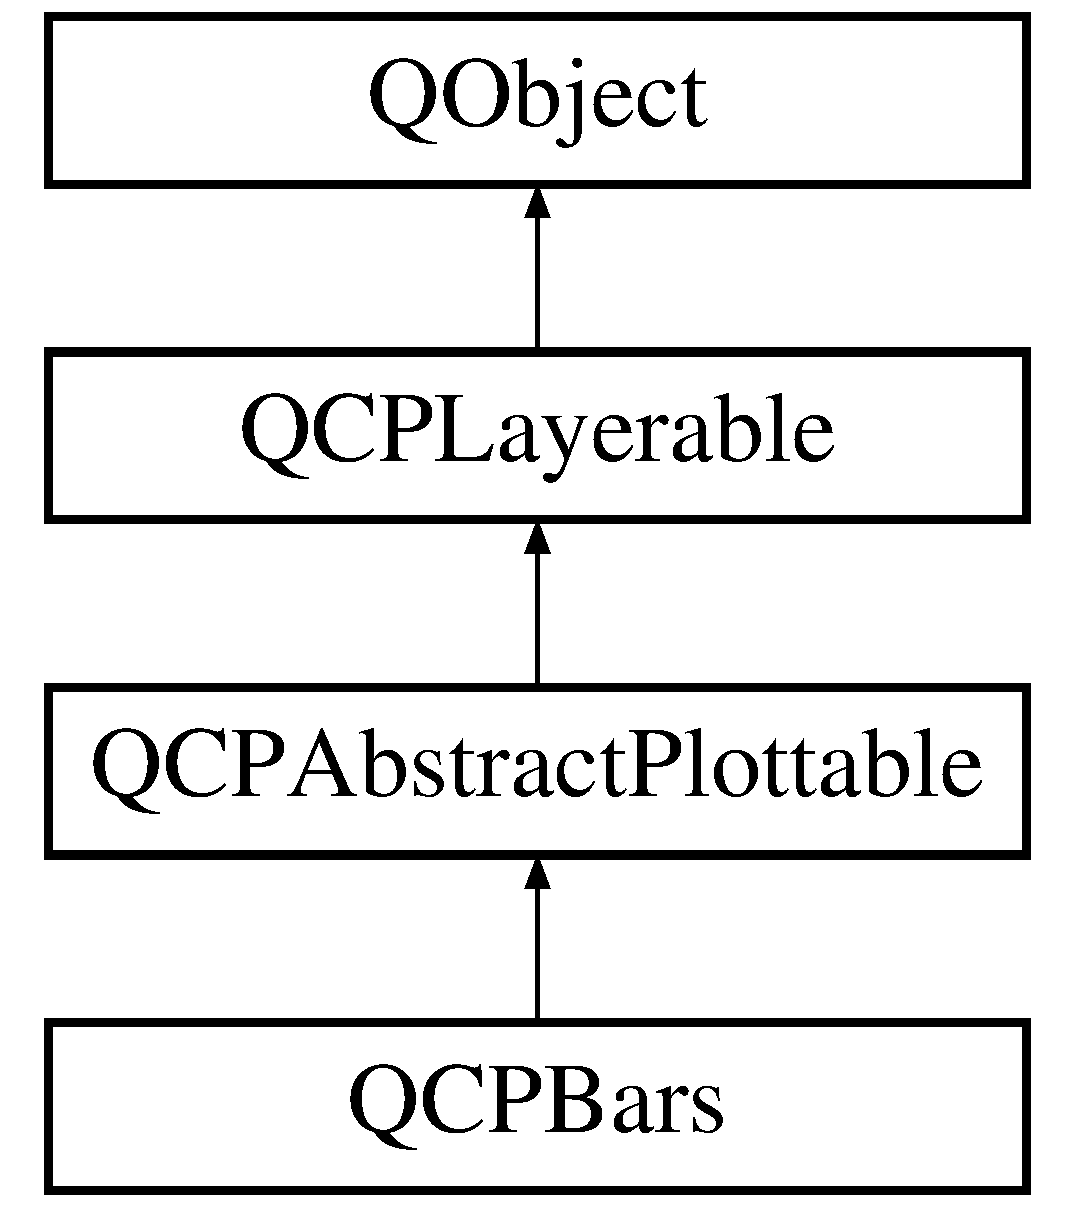
\includegraphics[height=4.000000cm]{class_q_c_p_bars}
\end{center}
\end{figure}
\subsection*{Public Types}
\begin{DoxyCompactItemize}
\item 
enum \hyperlink{class_q_c_p_bars_a65dbbf1ab41cbe993d71521096ed4649}{Width\+Type} \{ \hyperlink{class_q_c_p_bars_a65dbbf1ab41cbe993d71521096ed4649ab74315c9aa77df593c58dd25dfc0de35}{wt\+Absolute}, 
\hyperlink{class_q_c_p_bars_a65dbbf1ab41cbe993d71521096ed4649a90bc09899361ad3422ff277f7c790ffe}{wt\+Axis\+Rect\+Ratio}, 
\hyperlink{class_q_c_p_bars_a65dbbf1ab41cbe993d71521096ed4649aad3cc60ae1bfb1160a30237bee9eaf10}{wt\+Plot\+Coords}
 \}
\end{DoxyCompactItemize}
\subsection*{Public Member Functions}
\begin{DoxyCompactItemize}
\item 
\hyperlink{class_q_c_p_bars_a64006999ad9dff308f40df41cef176ad}{Q\+C\+P\+Bars} (\hyperlink{class_q_c_p_axis}{Q\+C\+P\+Axis} $\ast$key\+Axis, \hyperlink{class_q_c_p_axis}{Q\+C\+P\+Axis} $\ast$value\+Axis)
\item 
\hypertarget{class_q_c_p_bars_abe7eb3987d8711f45829db879aee2280}{}\label{class_q_c_p_bars_abe7eb3987d8711f45829db879aee2280} 
double {\bfseries width} () const
\item 
\hypertarget{class_q_c_p_bars_a4c103fb405a45f47853e0345f0c6e708}{}\label{class_q_c_p_bars_a4c103fb405a45f47853e0345f0c6e708} 
\hyperlink{class_q_c_p_bars_a65dbbf1ab41cbe993d71521096ed4649}{Width\+Type} {\bfseries width\+Type} () const
\item 
\hypertarget{class_q_c_p_bars_a5eef59840b68d205df4e0c3df5f97633}{}\label{class_q_c_p_bars_a5eef59840b68d205df4e0c3df5f97633} 
\hyperlink{class_q_c_p_bars_group}{Q\+C\+P\+Bars\+Group} $\ast$ {\bfseries bars\+Group} () const
\item 
\hypertarget{class_q_c_p_bars_a29a7b3b86f80b2a04bd1f9ec0ebaf422}{}\label{class_q_c_p_bars_a29a7b3b86f80b2a04bd1f9ec0ebaf422} 
double {\bfseries base\+Value} () const
\item 
\hyperlink{class_q_c_p_bars}{Q\+C\+P\+Bars} $\ast$ \hyperlink{class_q_c_p_bars_a1b58664864b141f45e02044a855b3213}{bar\+Below} () const
\item 
\hyperlink{class_q_c_p_bars}{Q\+C\+P\+Bars} $\ast$ \hyperlink{class_q_c_p_bars_ab97f2acd9f6cb40d2cc3c33d278f0e78}{bar\+Above} () const
\item 
\hypertarget{class_q_c_p_bars_a185bcee5f2d96fbc336a2d270687d016}{}\label{class_q_c_p_bars_a185bcee5f2d96fbc336a2d270687d016} 
\hyperlink{qcustomplot_8h_aa846c77472cae93def9f1609d0c57191}{Q\+C\+P\+Bar\+Data\+Map} $\ast$ {\bfseries data} () const
\item 
void \hyperlink{class_q_c_p_bars_afec6116579d44d5b706e0fa5e5332507}{set\+Width} (double width)
\item 
void \hyperlink{class_q_c_p_bars_adcaa3b41281bb2c0f7949b341592fcc0}{set\+Width\+Type} (\hyperlink{class_q_c_p_bars_a65dbbf1ab41cbe993d71521096ed4649}{Width\+Type} width\+Type)
\item 
void \hyperlink{class_q_c_p_bars_aedd1709061f0b307c47ddb45e172ef9a}{set\+Bars\+Group} (\hyperlink{class_q_c_p_bars_group}{Q\+C\+P\+Bars\+Group} $\ast$bars\+Group)
\item 
void \hyperlink{class_q_c_p_bars_a574ec7eb7537566df1a28ff085d75623}{set\+Base\+Value} (double base\+Value)
\item 
void \hyperlink{class_q_c_p_bars_aa3435aab19e0a49e4e7b41bd36a8d96b}{set\+Data} (\hyperlink{qcustomplot_8h_aa846c77472cae93def9f1609d0c57191}{Q\+C\+P\+Bar\+Data\+Map} $\ast$data, bool copy=false)
\item 
void \hyperlink{class_q_c_p_bars_a3efded5df4a82ecb201f7c28099fa2e5}{set\+Data} (const Q\+Vector$<$ double $>$ \&key, const Q\+Vector$<$ double $>$ \&value)
\item 
void \hyperlink{class_q_c_p_bars_a69fc371346980f19177c3d1ecdad78ee}{move\+Below} (\hyperlink{class_q_c_p_bars}{Q\+C\+P\+Bars} $\ast$bars)
\item 
void \hyperlink{class_q_c_p_bars_ac22e00a6a41509538c21b04f0a57318c}{move\+Above} (\hyperlink{class_q_c_p_bars}{Q\+C\+P\+Bars} $\ast$bars)
\item 
void \hyperlink{class_q_c_p_bars_a1f29cf08615040993209147fa68de3f2}{add\+Data} (const \hyperlink{qcustomplot_8h_aa846c77472cae93def9f1609d0c57191}{Q\+C\+P\+Bar\+Data\+Map} \&data\+Map)
\item 
void \hyperlink{class_q_c_p_bars_a142158b1addefd53259002dd3ab22c3a}{add\+Data} (const \hyperlink{class_q_c_p_bar_data}{Q\+C\+P\+Bar\+Data} \&data)
\item 
void \hyperlink{class_q_c_p_bars_a684dd105403a5497fda42f2094fecbb7}{add\+Data} (double key, double value)
\item 
void \hyperlink{class_q_c_p_bars_a3679a0a9decab0fa03f8f4c6e3344d52}{add\+Data} (const Q\+Vector$<$ double $>$ \&keys, const Q\+Vector$<$ double $>$ \&values)
\item 
void \hyperlink{class_q_c_p_bars_a9d12779a3fad4820aad2c428f368298d}{remove\+Data\+Before} (double key)
\item 
void \hyperlink{class_q_c_p_bars_a99de6e7abbbf03fb41fa604c7f08aa8b}{remove\+Data\+After} (double key)
\item 
void \hyperlink{class_q_c_p_bars_a1fe9bcb57d670defea1bb65cadf43765}{remove\+Data} (double from\+Key, double to\+Key)
\item 
void \hyperlink{class_q_c_p_bars_a837cc9848ad3edd40a6130b508493f93}{remove\+Data} (double key)
\item 
virtual void \hyperlink{class_q_c_p_bars_a11dbbd707132f07f862dff13c5789c2b}{clear\+Data} ()
\item 
virtual double \hyperlink{class_q_c_p_bars_a62d66cc8eedca6bedfc1f6513164d418}{select\+Test} (const Q\+PointF \&pos, bool only\+Selectable, Q\+Variant $\ast$details=0) const
\end{DoxyCompactItemize}
\subsection*{Protected Member Functions}
\begin{DoxyCompactItemize}
\item 
\hypertarget{class_q_c_p_bars_a42b894e34dac799f90ff3700706b31df}{}\label{class_q_c_p_bars_a42b894e34dac799f90ff3700706b31df} 
virtual void {\bfseries draw} (\hyperlink{class_q_c_p_painter}{Q\+C\+P\+Painter} $\ast$painter)
\item 
\hypertarget{class_q_c_p_bars_ad466f06b0fa561b6e12c92fdb8fa3c7f}{}\label{class_q_c_p_bars_ad466f06b0fa561b6e12c92fdb8fa3c7f} 
virtual void {\bfseries draw\+Legend\+Icon} (\hyperlink{class_q_c_p_painter}{Q\+C\+P\+Painter} $\ast$painter, const Q\+RectF \&rect) const
\item 
\hypertarget{class_q_c_p_bars_a0161ff6af64e025543c66130bcaa7ffd}{}\label{class_q_c_p_bars_a0161ff6af64e025543c66130bcaa7ffd} 
virtual \hyperlink{class_q_c_p_range}{Q\+C\+P\+Range} {\bfseries get\+Key\+Range} (bool \&found\+Range, \hyperlink{class_q_c_p_abstract_plottable_a661743478a1d3c09d28ec2711d7653d8}{Sign\+Domain} in\+Sign\+Domain=\hyperlink{class_q_c_p_abstract_plottable_a661743478a1d3c09d28ec2711d7653d8a082b98cfb91a7363a3b5cd17b0c1cd60}{sd\+Both}) const
\item 
\hypertarget{class_q_c_p_bars_af71b8e6ee0b800f0b79f2b6e692afee2}{}\label{class_q_c_p_bars_af71b8e6ee0b800f0b79f2b6e692afee2} 
virtual \hyperlink{class_q_c_p_range}{Q\+C\+P\+Range} {\bfseries get\+Value\+Range} (bool \&found\+Range, \hyperlink{class_q_c_p_abstract_plottable_a661743478a1d3c09d28ec2711d7653d8}{Sign\+Domain} in\+Sign\+Domain=\hyperlink{class_q_c_p_abstract_plottable_a661743478a1d3c09d28ec2711d7653d8a082b98cfb91a7363a3b5cd17b0c1cd60}{sd\+Both}) const
\item 
\hypertarget{class_q_c_p_bars_adce71831920cf0426722fdd47ba34261}{}\label{class_q_c_p_bars_adce71831920cf0426722fdd47ba34261} 
void {\bfseries get\+Visible\+Data\+Bounds} (Q\+C\+P\+Bar\+Data\+Map\+::const\+\_\+iterator \&lower, Q\+C\+P\+Bar\+Data\+Map\+::const\+\_\+iterator \&upper\+End) const
\item 
\hypertarget{class_q_c_p_bars_a3a4ca0069f003929284763caef1856a8}{}\label{class_q_c_p_bars_a3a4ca0069f003929284763caef1856a8} 
Q\+PolygonF {\bfseries get\+Bar\+Polygon} (double key, double value) const
\item 
\hypertarget{class_q_c_p_bars_ad87586cc5e9806740bc0e867667da409}{}\label{class_q_c_p_bars_ad87586cc5e9806740bc0e867667da409} 
void {\bfseries get\+Pixel\+Width} (double key, double \&lower, double \&upper) const
\item 
\hypertarget{class_q_c_p_bars_a0ffd6e043876e13e89eaa54e9f8a04b9}{}\label{class_q_c_p_bars_a0ffd6e043876e13e89eaa54e9f8a04b9} 
double {\bfseries get\+Stacked\+Base\+Value} (double key, bool positive) const
\end{DoxyCompactItemize}
\subsection*{Static Protected Member Functions}
\begin{DoxyCompactItemize}
\item 
\hypertarget{class_q_c_p_bars_a6ea37802cd22f97235cab614b14b9f19}{}\label{class_q_c_p_bars_a6ea37802cd22f97235cab614b14b9f19} 
static void {\bfseries connect\+Bars} (\hyperlink{class_q_c_p_bars}{Q\+C\+P\+Bars} $\ast$lower, \hyperlink{class_q_c_p_bars}{Q\+C\+P\+Bars} $\ast$upper)
\end{DoxyCompactItemize}
\subsection*{Protected Attributes}
\begin{DoxyCompactItemize}
\item 
\hypertarget{class_q_c_p_bars_aef28d29d51ef84b608ecd22c55d531ff}{}\label{class_q_c_p_bars_aef28d29d51ef84b608ecd22c55d531ff} 
\hyperlink{qcustomplot_8h_aa846c77472cae93def9f1609d0c57191}{Q\+C\+P\+Bar\+Data\+Map} $\ast$ {\bfseries m\+Data}
\item 
\hypertarget{class_q_c_p_bars_a7c4e0f2246f8133f48a9c3f24cf5b920}{}\label{class_q_c_p_bars_a7c4e0f2246f8133f48a9c3f24cf5b920} 
double {\bfseries m\+Width}
\item 
\hypertarget{class_q_c_p_bars_a94dba1309496c7601d01e2c59715cbb3}{}\label{class_q_c_p_bars_a94dba1309496c7601d01e2c59715cbb3} 
\hyperlink{class_q_c_p_bars_a65dbbf1ab41cbe993d71521096ed4649}{Width\+Type} {\bfseries m\+Width\+Type}
\item 
\hypertarget{class_q_c_p_bars_a9f59c255f3739182ca9744dff75beaa9}{}\label{class_q_c_p_bars_a9f59c255f3739182ca9744dff75beaa9} 
\hyperlink{class_q_c_p_bars_group}{Q\+C\+P\+Bars\+Group} $\ast$ {\bfseries m\+Bars\+Group}
\item 
\hypertarget{class_q_c_p_bars_aa0515cf47fa6044cc28e59b1ae5ec759}{}\label{class_q_c_p_bars_aa0515cf47fa6044cc28e59b1ae5ec759} 
double {\bfseries m\+Base\+Value}
\item 
\hypertarget{class_q_c_p_bars_ad51db970eed7e286f2753b0216fc56de}{}\label{class_q_c_p_bars_ad51db970eed7e286f2753b0216fc56de} 
Q\+Pointer$<$ \hyperlink{class_q_c_p_bars}{Q\+C\+P\+Bars} $>$ {\bfseries m\+Bar\+Below}
\item 
\hypertarget{class_q_c_p_bars_a0c1c46076c41a478dbb373cfd35929aa}{}\label{class_q_c_p_bars_a0c1c46076c41a478dbb373cfd35929aa} 
Q\+Pointer$<$ \hyperlink{class_q_c_p_bars}{Q\+C\+P\+Bars} $>$ {\bfseries m\+Bar\+Above}
\end{DoxyCompactItemize}
\subsection*{Friends}
\begin{DoxyCompactItemize}
\item 
\hypertarget{class_q_c_p_bars_a1cdf9df76adcfae45261690aa0ca2198}{}\label{class_q_c_p_bars_a1cdf9df76adcfae45261690aa0ca2198} 
class {\bfseries Q\+Custom\+Plot}
\item 
\hypertarget{class_q_c_p_bars_a8429035e7adfbd7f05805a6530ad5e3b}{}\label{class_q_c_p_bars_a8429035e7adfbd7f05805a6530ad5e3b} 
class {\bfseries Q\+C\+P\+Legend}
\item 
\hypertarget{class_q_c_p_bars_ae1051b4d58a2786cb420367a586e2fee}{}\label{class_q_c_p_bars_ae1051b4d58a2786cb420367a586e2fee} 
class {\bfseries Q\+C\+P\+Bars\+Group}
\end{DoxyCompactItemize}
\subsection*{Additional Inherited Members}


\subsection{Detailed Description}
A plottable representing a bar chart in a plot. 



To plot data, assign it with the \hyperlink{class_q_c_p_bars_aa3435aab19e0a49e4e7b41bd36a8d96b}{set\+Data} or \hyperlink{class_q_c_p_bars_a1f29cf08615040993209147fa68de3f2}{add\+Data} functions.\hypertarget{class_q_c_p_statistical_box_appearance}{}\subsection{Changing the appearance}\label{class_q_c_p_statistical_box_appearance}
The appearance of the bars is determined by the pen and the brush (\hyperlink{class_q_c_p_abstract_plottable_ab74b09ae4c0e7e13142fe4b5bf46cac7}{set\+Pen}, \hyperlink{class_q_c_p_abstract_plottable_a7a4b92144dca6453a1f0f210e27edc74}{set\+Brush}). The width of the individual bars can be controlled with \hyperlink{class_q_c_p_bars_adcaa3b41281bb2c0f7949b341592fcc0}{set\+Width\+Type} and \hyperlink{class_q_c_p_bars_afec6116579d44d5b706e0fa5e5332507}{set\+Width}.

Bar charts are stackable. This means, two \hyperlink{class_q_c_p_bars}{Q\+C\+P\+Bars} plottables can be placed on top of each other (see \hyperlink{class_q_c_p_bars_ac22e00a6a41509538c21b04f0a57318c}{Q\+C\+P\+Bars\+::move\+Above}). So when two bars are at the same key position, they will appear stacked.

If you would like to group multiple \hyperlink{class_q_c_p_bars}{Q\+C\+P\+Bars} plottables together so they appear side by side as shown below, use \hyperlink{class_q_c_p_bars_group}{Q\+C\+P\+Bars\+Group}.

\hypertarget{class_q_c_p_statistical_box_usage}{}\subsection{Usage}\label{class_q_c_p_statistical_box_usage}
Like all data representing objects in \hyperlink{class_q_custom_plot}{Q\+Custom\+Plot}, the \hyperlink{class_q_c_p_bars}{Q\+C\+P\+Bars} is a plottable (\hyperlink{class_q_c_p_abstract_plottable}{Q\+C\+P\+Abstract\+Plottable}). So the plottable-\/interface of \hyperlink{class_q_custom_plot}{Q\+Custom\+Plot} applies (\hyperlink{class_q_custom_plot_a32de81ff53e263e785b83b52ecd99d6f}{Q\+Custom\+Plot\+::plottable}, \hyperlink{class_q_custom_plot_ab7ad9174f701f9c6f64e378df77927a6}{Q\+Custom\+Plot\+::add\+Plottable}, \hyperlink{class_q_custom_plot_af3dafd56884208474f311d6226513ab2}{Q\+Custom\+Plot\+::remove\+Plottable}, etc.)

Usually, you first create an instance\+: 
\begin{DoxyCodeInclude}
\end{DoxyCodeInclude}
add it to the custom\+Plot with \hyperlink{class_q_custom_plot_ab7ad9174f701f9c6f64e378df77927a6}{Q\+Custom\+Plot\+::add\+Plottable}\+: 
\begin{DoxyCodeInclude}
\end{DoxyCodeInclude}
and then modify the properties of the newly created plottable, e.\+g.\+: 
\begin{DoxyCodeInclude}
\end{DoxyCodeInclude}


\subsection{Member Enumeration Documentation}
\hypertarget{class_q_c_p_bars_a65dbbf1ab41cbe993d71521096ed4649}{}\label{class_q_c_p_bars_a65dbbf1ab41cbe993d71521096ed4649} 
\index{Q\+C\+P\+Bars@{Q\+C\+P\+Bars}!Width\+Type@{Width\+Type}}
\index{Width\+Type@{Width\+Type}!Q\+C\+P\+Bars@{Q\+C\+P\+Bars}}
\subsubsection{\texorpdfstring{Width\+Type}{WidthType}}
{\footnotesize\ttfamily enum \hyperlink{class_q_c_p_bars_a65dbbf1ab41cbe993d71521096ed4649}{Q\+C\+P\+Bars\+::\+Width\+Type}}

Defines the ways the width of the bar can be specified. Thus it defines what the number passed to \hyperlink{class_q_c_p_bars_afec6116579d44d5b706e0fa5e5332507}{set\+Width} actually means.

\begin{DoxySeeAlso}{See also}
\hyperlink{class_q_c_p_bars_adcaa3b41281bb2c0f7949b341592fcc0}{set\+Width\+Type}, \hyperlink{class_q_c_p_bars_afec6116579d44d5b706e0fa5e5332507}{set\+Width} 
\end{DoxySeeAlso}
\begin{DoxyEnumFields}{Enumerator}
\raisebox{\heightof{T}}[0pt][0pt]{\index{wt\+Absolute@{wt\+Absolute}!Q\+C\+P\+Bars@{Q\+C\+P\+Bars}}\index{Q\+C\+P\+Bars@{Q\+C\+P\+Bars}!wt\+Absolute@{wt\+Absolute}}}\hypertarget{class_q_c_p_bars_a65dbbf1ab41cbe993d71521096ed4649ab74315c9aa77df593c58dd25dfc0de35}{}\label{class_q_c_p_bars_a65dbbf1ab41cbe993d71521096ed4649ab74315c9aa77df593c58dd25dfc0de35} 
wt\+Absolute&Bar width is in absolute pixels. \\
\hline

\raisebox{\heightof{T}}[0pt][0pt]{\index{wt\+Axis\+Rect\+Ratio@{wt\+Axis\+Rect\+Ratio}!Q\+C\+P\+Bars@{Q\+C\+P\+Bars}}\index{Q\+C\+P\+Bars@{Q\+C\+P\+Bars}!wt\+Axis\+Rect\+Ratio@{wt\+Axis\+Rect\+Ratio}}}\hypertarget{class_q_c_p_bars_a65dbbf1ab41cbe993d71521096ed4649a90bc09899361ad3422ff277f7c790ffe}{}\label{class_q_c_p_bars_a65dbbf1ab41cbe993d71521096ed4649a90bc09899361ad3422ff277f7c790ffe} 
wt\+Axis\+Rect\+Ratio&Bar width is given by a fraction of the axis rect size. \\
\hline

\raisebox{\heightof{T}}[0pt][0pt]{\index{wt\+Plot\+Coords@{wt\+Plot\+Coords}!Q\+C\+P\+Bars@{Q\+C\+P\+Bars}}\index{Q\+C\+P\+Bars@{Q\+C\+P\+Bars}!wt\+Plot\+Coords@{wt\+Plot\+Coords}}}\hypertarget{class_q_c_p_bars_a65dbbf1ab41cbe993d71521096ed4649aad3cc60ae1bfb1160a30237bee9eaf10}{}\label{class_q_c_p_bars_a65dbbf1ab41cbe993d71521096ed4649aad3cc60ae1bfb1160a30237bee9eaf10} 
wt\+Plot\+Coords&Bar width is in key coordinates and thus scales with the key axis range. \\
\hline

\end{DoxyEnumFields}


\subsection{Constructor \& Destructor Documentation}
\hypertarget{class_q_c_p_bars_a64006999ad9dff308f40df41cef176ad}{}\label{class_q_c_p_bars_a64006999ad9dff308f40df41cef176ad} 
\index{Q\+C\+P\+Bars@{Q\+C\+P\+Bars}!Q\+C\+P\+Bars@{Q\+C\+P\+Bars}}
\index{Q\+C\+P\+Bars@{Q\+C\+P\+Bars}!Q\+C\+P\+Bars@{Q\+C\+P\+Bars}}
\subsubsection{\texorpdfstring{Q\+C\+P\+Bars()}{QCPBars()}}
{\footnotesize\ttfamily Q\+C\+P\+Bars\+::\+Q\+C\+P\+Bars (\begin{DoxyParamCaption}\item[{\hyperlink{class_q_c_p_axis}{Q\+C\+P\+Axis} $\ast$}]{key\+Axis,  }\item[{\hyperlink{class_q_c_p_axis}{Q\+C\+P\+Axis} $\ast$}]{value\+Axis }\end{DoxyParamCaption})\hspace{0.3cm}{\ttfamily [explicit]}}

Constructs a bar chart which uses {\itshape key\+Axis} as its key axis (\char`\"{}x\char`\"{}) and {\itshape value\+Axis} as its value axis (\char`\"{}y\char`\"{}). {\itshape key\+Axis} and {\itshape value\+Axis} must reside in the same \hyperlink{class_q_custom_plot}{Q\+Custom\+Plot} instance and not have the same orientation. If either of these restrictions is violated, a corresponding message is printed to the debug output (q\+Debug), the construction is not aborted, though.

The constructed \hyperlink{class_q_c_p_bars}{Q\+C\+P\+Bars} can be added to the plot with \hyperlink{class_q_custom_plot_ab7ad9174f701f9c6f64e378df77927a6}{Q\+Custom\+Plot\+::add\+Plottable}, \hyperlink{class_q_custom_plot}{Q\+Custom\+Plot} then takes ownership of the bar chart. 

\subsection{Member Function Documentation}
\hypertarget{class_q_c_p_bars_a1f29cf08615040993209147fa68de3f2}{}\label{class_q_c_p_bars_a1f29cf08615040993209147fa68de3f2} 
\index{Q\+C\+P\+Bars@{Q\+C\+P\+Bars}!add\+Data@{add\+Data}}
\index{add\+Data@{add\+Data}!Q\+C\+P\+Bars@{Q\+C\+P\+Bars}}
\subsubsection{\texorpdfstring{add\+Data()}{addData()}\hspace{0.1cm}{\footnotesize\ttfamily [1/4]}}
{\footnotesize\ttfamily void Q\+C\+P\+Bars\+::add\+Data (\begin{DoxyParamCaption}\item[{const \hyperlink{qcustomplot_8h_aa846c77472cae93def9f1609d0c57191}{Q\+C\+P\+Bar\+Data\+Map} \&}]{data\+Map }\end{DoxyParamCaption})}

Adds the provided data points in {\itshape data\+Map} to the current data. \begin{DoxySeeAlso}{See also}
\hyperlink{class_q_c_p_bars_a1fe9bcb57d670defea1bb65cadf43765}{remove\+Data} 
\end{DoxySeeAlso}
\hypertarget{class_q_c_p_bars_a142158b1addefd53259002dd3ab22c3a}{}\label{class_q_c_p_bars_a142158b1addefd53259002dd3ab22c3a} 
\index{Q\+C\+P\+Bars@{Q\+C\+P\+Bars}!add\+Data@{add\+Data}}
\index{add\+Data@{add\+Data}!Q\+C\+P\+Bars@{Q\+C\+P\+Bars}}
\subsubsection{\texorpdfstring{add\+Data()}{addData()}\hspace{0.1cm}{\footnotesize\ttfamily [2/4]}}
{\footnotesize\ttfamily void Q\+C\+P\+Bars\+::add\+Data (\begin{DoxyParamCaption}\item[{const \hyperlink{class_q_c_p_bar_data}{Q\+C\+P\+Bar\+Data} \&}]{data }\end{DoxyParamCaption})}

This is an overloaded member function, provided for convenience. It differs from the above function only in what argument(s) it accepts. Adds the provided single data point in {\itshape data} to the current data. \begin{DoxySeeAlso}{See also}
\hyperlink{class_q_c_p_bars_a1fe9bcb57d670defea1bb65cadf43765}{remove\+Data} 
\end{DoxySeeAlso}
\hypertarget{class_q_c_p_bars_a684dd105403a5497fda42f2094fecbb7}{}\label{class_q_c_p_bars_a684dd105403a5497fda42f2094fecbb7} 
\index{Q\+C\+P\+Bars@{Q\+C\+P\+Bars}!add\+Data@{add\+Data}}
\index{add\+Data@{add\+Data}!Q\+C\+P\+Bars@{Q\+C\+P\+Bars}}
\subsubsection{\texorpdfstring{add\+Data()}{addData()}\hspace{0.1cm}{\footnotesize\ttfamily [3/4]}}
{\footnotesize\ttfamily void Q\+C\+P\+Bars\+::add\+Data (\begin{DoxyParamCaption}\item[{double}]{key,  }\item[{double}]{value }\end{DoxyParamCaption})}

This is an overloaded member function, provided for convenience. It differs from the above function only in what argument(s) it accepts. Adds the provided single data point as {\itshape key} and {\itshape value} tuple to the current data \begin{DoxySeeAlso}{See also}
\hyperlink{class_q_c_p_bars_a1fe9bcb57d670defea1bb65cadf43765}{remove\+Data} 
\end{DoxySeeAlso}
\hypertarget{class_q_c_p_bars_a3679a0a9decab0fa03f8f4c6e3344d52}{}\label{class_q_c_p_bars_a3679a0a9decab0fa03f8f4c6e3344d52} 
\index{Q\+C\+P\+Bars@{Q\+C\+P\+Bars}!add\+Data@{add\+Data}}
\index{add\+Data@{add\+Data}!Q\+C\+P\+Bars@{Q\+C\+P\+Bars}}
\subsubsection{\texorpdfstring{add\+Data()}{addData()}\hspace{0.1cm}{\footnotesize\ttfamily [4/4]}}
{\footnotesize\ttfamily void Q\+C\+P\+Bars\+::add\+Data (\begin{DoxyParamCaption}\item[{const Q\+Vector$<$ double $>$ \&}]{keys,  }\item[{const Q\+Vector$<$ double $>$ \&}]{values }\end{DoxyParamCaption})}

This is an overloaded member function, provided for convenience. It differs from the above function only in what argument(s) it accepts. Adds the provided data points as {\itshape key} and {\itshape value} tuples to the current data. \begin{DoxySeeAlso}{See also}
\hyperlink{class_q_c_p_bars_a1fe9bcb57d670defea1bb65cadf43765}{remove\+Data} 
\end{DoxySeeAlso}
\hypertarget{class_q_c_p_bars_ab97f2acd9f6cb40d2cc3c33d278f0e78}{}\label{class_q_c_p_bars_ab97f2acd9f6cb40d2cc3c33d278f0e78} 
\index{Q\+C\+P\+Bars@{Q\+C\+P\+Bars}!bar\+Above@{bar\+Above}}
\index{bar\+Above@{bar\+Above}!Q\+C\+P\+Bars@{Q\+C\+P\+Bars}}
\subsubsection{\texorpdfstring{bar\+Above()}{barAbove()}}
{\footnotesize\ttfamily \hyperlink{class_q_c_p_bars}{Q\+C\+P\+Bars} $\ast$ Q\+C\+P\+Bars\+::bar\+Above (\begin{DoxyParamCaption}{ }\end{DoxyParamCaption}) const\hspace{0.3cm}{\ttfamily [inline]}}

Returns the bars plottable that is directly above this bars plottable. If there is no such plottable, returns 0.

\begin{DoxySeeAlso}{See also}
\hyperlink{class_q_c_p_bars_a1b58664864b141f45e02044a855b3213}{bar\+Below}, \hyperlink{class_q_c_p_bars_a69fc371346980f19177c3d1ecdad78ee}{move\+Below}, \hyperlink{class_q_c_p_bars_ac22e00a6a41509538c21b04f0a57318c}{move\+Above} 
\end{DoxySeeAlso}
\hypertarget{class_q_c_p_bars_a1b58664864b141f45e02044a855b3213}{}\label{class_q_c_p_bars_a1b58664864b141f45e02044a855b3213} 
\index{Q\+C\+P\+Bars@{Q\+C\+P\+Bars}!bar\+Below@{bar\+Below}}
\index{bar\+Below@{bar\+Below}!Q\+C\+P\+Bars@{Q\+C\+P\+Bars}}
\subsubsection{\texorpdfstring{bar\+Below()}{barBelow()}}
{\footnotesize\ttfamily \hyperlink{class_q_c_p_bars}{Q\+C\+P\+Bars} $\ast$ Q\+C\+P\+Bars\+::bar\+Below (\begin{DoxyParamCaption}{ }\end{DoxyParamCaption}) const\hspace{0.3cm}{\ttfamily [inline]}}

Returns the bars plottable that is directly below this bars plottable. If there is no such plottable, returns 0.

\begin{DoxySeeAlso}{See also}
\hyperlink{class_q_c_p_bars_ab97f2acd9f6cb40d2cc3c33d278f0e78}{bar\+Above}, \hyperlink{class_q_c_p_bars_a69fc371346980f19177c3d1ecdad78ee}{move\+Below}, \hyperlink{class_q_c_p_bars_ac22e00a6a41509538c21b04f0a57318c}{move\+Above} 
\end{DoxySeeAlso}
\hypertarget{class_q_c_p_bars_a11dbbd707132f07f862dff13c5789c2b}{}\label{class_q_c_p_bars_a11dbbd707132f07f862dff13c5789c2b} 
\index{Q\+C\+P\+Bars@{Q\+C\+P\+Bars}!clear\+Data@{clear\+Data}}
\index{clear\+Data@{clear\+Data}!Q\+C\+P\+Bars@{Q\+C\+P\+Bars}}
\subsubsection{\texorpdfstring{clear\+Data()}{clearData()}}
{\footnotesize\ttfamily void Q\+C\+P\+Bars\+::clear\+Data (\begin{DoxyParamCaption}{ }\end{DoxyParamCaption})\hspace{0.3cm}{\ttfamily [virtual]}}

Removes all data points. \begin{DoxySeeAlso}{See also}
\hyperlink{class_q_c_p_bars_a1fe9bcb57d670defea1bb65cadf43765}{remove\+Data}, \hyperlink{class_q_c_p_bars_a99de6e7abbbf03fb41fa604c7f08aa8b}{remove\+Data\+After}, \hyperlink{class_q_c_p_bars_a9d12779a3fad4820aad2c428f368298d}{remove\+Data\+Before} 
\end{DoxySeeAlso}


Implements \hyperlink{class_q_c_p_abstract_plottable_a86e5b8fd4b6ff4f4084e7ea4c573fc53}{Q\+C\+P\+Abstract\+Plottable}.

\hypertarget{class_q_c_p_bars_ac22e00a6a41509538c21b04f0a57318c}{}\label{class_q_c_p_bars_ac22e00a6a41509538c21b04f0a57318c} 
\index{Q\+C\+P\+Bars@{Q\+C\+P\+Bars}!move\+Above@{move\+Above}}
\index{move\+Above@{move\+Above}!Q\+C\+P\+Bars@{Q\+C\+P\+Bars}}
\subsubsection{\texorpdfstring{move\+Above()}{moveAbove()}}
{\footnotesize\ttfamily void Q\+C\+P\+Bars\+::move\+Above (\begin{DoxyParamCaption}\item[{\hyperlink{class_q_c_p_bars}{Q\+C\+P\+Bars} $\ast$}]{bars }\end{DoxyParamCaption})}

Moves this bars plottable above {\itshape bars}. In other words, the bars of this plottable will appear above the bars of {\itshape bars}. The move target {\itshape bars} must use the same key and value axis as this plottable.

Inserting into and removing from existing bar stacking is handled gracefully. If {\itshape bars} already has a bars object above itself, this bars object is inserted between the two. If this bars object is already between two other bars, the two other bars will be stacked on top of each other after the operation.

To remove this bars plottable from any stacking, set {\itshape bars} to 0.

\begin{DoxySeeAlso}{See also}
\hyperlink{class_q_c_p_bars_a69fc371346980f19177c3d1ecdad78ee}{move\+Below}, \hyperlink{class_q_c_p_bars_a1b58664864b141f45e02044a855b3213}{bar\+Below}, \hyperlink{class_q_c_p_bars_ab97f2acd9f6cb40d2cc3c33d278f0e78}{bar\+Above} 
\end{DoxySeeAlso}
\hypertarget{class_q_c_p_bars_a69fc371346980f19177c3d1ecdad78ee}{}\label{class_q_c_p_bars_a69fc371346980f19177c3d1ecdad78ee} 
\index{Q\+C\+P\+Bars@{Q\+C\+P\+Bars}!move\+Below@{move\+Below}}
\index{move\+Below@{move\+Below}!Q\+C\+P\+Bars@{Q\+C\+P\+Bars}}
\subsubsection{\texorpdfstring{move\+Below()}{moveBelow()}}
{\footnotesize\ttfamily void Q\+C\+P\+Bars\+::move\+Below (\begin{DoxyParamCaption}\item[{\hyperlink{class_q_c_p_bars}{Q\+C\+P\+Bars} $\ast$}]{bars }\end{DoxyParamCaption})}

Moves this bars plottable below {\itshape bars}. In other words, the bars of this plottable will appear below the bars of {\itshape bars}. The move target {\itshape bars} must use the same key and value axis as this plottable.

Inserting into and removing from existing bar stacking is handled gracefully. If {\itshape bars} already has a bars object below itself, this bars object is inserted between the two. If this bars object is already between two other bars, the two other bars will be stacked on top of each other after the operation.

To remove this bars plottable from any stacking, set {\itshape bars} to 0.

\begin{DoxySeeAlso}{See also}
\hyperlink{class_q_c_p_bars_a69fc371346980f19177c3d1ecdad78ee}{move\+Below}, \hyperlink{class_q_c_p_bars_ab97f2acd9f6cb40d2cc3c33d278f0e78}{bar\+Above}, \hyperlink{class_q_c_p_bars_a1b58664864b141f45e02044a855b3213}{bar\+Below} 
\end{DoxySeeAlso}
\hypertarget{class_q_c_p_bars_a1fe9bcb57d670defea1bb65cadf43765}{}\label{class_q_c_p_bars_a1fe9bcb57d670defea1bb65cadf43765} 
\index{Q\+C\+P\+Bars@{Q\+C\+P\+Bars}!remove\+Data@{remove\+Data}}
\index{remove\+Data@{remove\+Data}!Q\+C\+P\+Bars@{Q\+C\+P\+Bars}}
\subsubsection{\texorpdfstring{remove\+Data()}{removeData()}\hspace{0.1cm}{\footnotesize\ttfamily [1/2]}}
{\footnotesize\ttfamily void Q\+C\+P\+Bars\+::remove\+Data (\begin{DoxyParamCaption}\item[{double}]{from\+Key,  }\item[{double}]{to\+Key }\end{DoxyParamCaption})}

Removes all data points with key between {\itshape from\+Key} and {\itshape to\+Key}. if {\itshape from\+Key} is greater or equal to {\itshape to\+Key}, the function does nothing. To remove a single data point with known key, use \hyperlink{class_q_c_p_bars_a837cc9848ad3edd40a6130b508493f93}{remove\+Data(double key)}.

\begin{DoxySeeAlso}{See also}
\hyperlink{class_q_c_p_bars_a1f29cf08615040993209147fa68de3f2}{add\+Data}, \hyperlink{class_q_c_p_bars_a11dbbd707132f07f862dff13c5789c2b}{clear\+Data} 
\end{DoxySeeAlso}
\hypertarget{class_q_c_p_bars_a837cc9848ad3edd40a6130b508493f93}{}\label{class_q_c_p_bars_a837cc9848ad3edd40a6130b508493f93} 
\index{Q\+C\+P\+Bars@{Q\+C\+P\+Bars}!remove\+Data@{remove\+Data}}
\index{remove\+Data@{remove\+Data}!Q\+C\+P\+Bars@{Q\+C\+P\+Bars}}
\subsubsection{\texorpdfstring{remove\+Data()}{removeData()}\hspace{0.1cm}{\footnotesize\ttfamily [2/2]}}
{\footnotesize\ttfamily void Q\+C\+P\+Bars\+::remove\+Data (\begin{DoxyParamCaption}\item[{double}]{key }\end{DoxyParamCaption})}

This is an overloaded member function, provided for convenience. It differs from the above function only in what argument(s) it accepts.

Removes a single data point at {\itshape key}. If the position is not known with absolute precision, consider using \hyperlink{class_q_c_p_bars_a1fe9bcb57d670defea1bb65cadf43765}{remove\+Data(double from\+Key, double to\+Key)} with a small fuzziness interval around the suspected position, depeding on the precision with which the key is known.

\begin{DoxySeeAlso}{See also}
\hyperlink{class_q_c_p_bars_a1f29cf08615040993209147fa68de3f2}{add\+Data}, \hyperlink{class_q_c_p_bars_a11dbbd707132f07f862dff13c5789c2b}{clear\+Data} 
\end{DoxySeeAlso}
\hypertarget{class_q_c_p_bars_a99de6e7abbbf03fb41fa604c7f08aa8b}{}\label{class_q_c_p_bars_a99de6e7abbbf03fb41fa604c7f08aa8b} 
\index{Q\+C\+P\+Bars@{Q\+C\+P\+Bars}!remove\+Data\+After@{remove\+Data\+After}}
\index{remove\+Data\+After@{remove\+Data\+After}!Q\+C\+P\+Bars@{Q\+C\+P\+Bars}}
\subsubsection{\texorpdfstring{remove\+Data\+After()}{removeDataAfter()}}
{\footnotesize\ttfamily void Q\+C\+P\+Bars\+::remove\+Data\+After (\begin{DoxyParamCaption}\item[{double}]{key }\end{DoxyParamCaption})}

Removes all data points with key greater than {\itshape key}. \begin{DoxySeeAlso}{See also}
\hyperlink{class_q_c_p_bars_a1f29cf08615040993209147fa68de3f2}{add\+Data}, \hyperlink{class_q_c_p_bars_a11dbbd707132f07f862dff13c5789c2b}{clear\+Data} 
\end{DoxySeeAlso}
\hypertarget{class_q_c_p_bars_a9d12779a3fad4820aad2c428f368298d}{}\label{class_q_c_p_bars_a9d12779a3fad4820aad2c428f368298d} 
\index{Q\+C\+P\+Bars@{Q\+C\+P\+Bars}!remove\+Data\+Before@{remove\+Data\+Before}}
\index{remove\+Data\+Before@{remove\+Data\+Before}!Q\+C\+P\+Bars@{Q\+C\+P\+Bars}}
\subsubsection{\texorpdfstring{remove\+Data\+Before()}{removeDataBefore()}}
{\footnotesize\ttfamily void Q\+C\+P\+Bars\+::remove\+Data\+Before (\begin{DoxyParamCaption}\item[{double}]{key }\end{DoxyParamCaption})}

Removes all data points with key smaller than {\itshape key}. \begin{DoxySeeAlso}{See also}
\hyperlink{class_q_c_p_bars_a1f29cf08615040993209147fa68de3f2}{add\+Data}, \hyperlink{class_q_c_p_bars_a11dbbd707132f07f862dff13c5789c2b}{clear\+Data} 
\end{DoxySeeAlso}
\hypertarget{class_q_c_p_bars_a62d66cc8eedca6bedfc1f6513164d418}{}\label{class_q_c_p_bars_a62d66cc8eedca6bedfc1f6513164d418} 
\index{Q\+C\+P\+Bars@{Q\+C\+P\+Bars}!select\+Test@{select\+Test}}
\index{select\+Test@{select\+Test}!Q\+C\+P\+Bars@{Q\+C\+P\+Bars}}
\subsubsection{\texorpdfstring{select\+Test()}{selectTest()}}
{\footnotesize\ttfamily double Q\+C\+P\+Bars\+::select\+Test (\begin{DoxyParamCaption}\item[{const Q\+PointF \&}]{pos,  }\item[{bool}]{only\+Selectable,  }\item[{Q\+Variant $\ast$}]{details = {\ttfamily 0} }\end{DoxyParamCaption}) const\hspace{0.3cm}{\ttfamily [virtual]}}

This function is used to decide whether a click hits a layerable object or not.

{\itshape pos} is a point in pixel coordinates on the \hyperlink{class_q_custom_plot}{Q\+Custom\+Plot} surface. This function returns the shortest pixel distance of this point to the object. If the object is either invisible or the distance couldn\textquotesingle{}t be determined, -\/1.\+0 is returned. Further, if {\itshape only\+Selectable} is true and the object is not selectable, -\/1.\+0 is returned, too.

If the object is represented not by single lines but by an area like a \hyperlink{class_q_c_p_item_text}{Q\+C\+P\+Item\+Text} or the bars of a \hyperlink{class_q_c_p_bars}{Q\+C\+P\+Bars} plottable, a click inside the area should also be considered a hit. In these cases this function thus returns a constant value greater zero but still below the parent plot\textquotesingle{}s selection tolerance. (typically the selection\+Tolerance multiplied by 0.\+99).

Providing a constant value for area objects allows selecting line objects even when they are obscured by such area objects, by clicking close to the lines (i.\+e. closer than 0.\+99$\ast$selection\+Tolerance).

The actual setting of the selection state is not done by this function. This is handled by the parent \hyperlink{class_q_custom_plot}{Q\+Custom\+Plot} when the mouse\+Release\+Event occurs, and the finally selected object is notified via the select\+Event/deselect\+Event methods.

{\itshape details} is an optional output parameter. Every layerable subclass may place any information in {\itshape details}. This information will be passed to select\+Event when the parent \hyperlink{class_q_custom_plot}{Q\+Custom\+Plot} decides on the basis of this select\+Test call, that the object was successfully selected. The subsequent call to select\+Event will carry the {\itshape details}. This is useful for multi-\/part objects (like \hyperlink{class_q_c_p_axis}{Q\+C\+P\+Axis}). This way, a possibly complex calculation to decide which part was clicked is only done once in \hyperlink{class_q_c_p_bars_a62d66cc8eedca6bedfc1f6513164d418}{select\+Test}. The result (i.\+e. the actually clicked part) can then be placed in {\itshape details}. So in the subsequent select\+Event, the decision which part was selected doesn\textquotesingle{}t have to be done a second time for a single selection operation.

You may pass 0 as {\itshape details} to indicate that you are not interested in those selection details.

\begin{DoxySeeAlso}{See also}
select\+Event, deselect\+Event, \hyperlink{class_q_custom_plot_a5ee1e2f6ae27419deca53e75907c27e5}{Q\+Custom\+Plot\+::set\+Interactions} 
\end{DoxySeeAlso}


Implements \hyperlink{class_q_c_p_abstract_plottable_a38efe9641d972992a3d44204bc80ec1d}{Q\+C\+P\+Abstract\+Plottable}.

\hypertarget{class_q_c_p_bars_aedd1709061f0b307c47ddb45e172ef9a}{}\label{class_q_c_p_bars_aedd1709061f0b307c47ddb45e172ef9a} 
\index{Q\+C\+P\+Bars@{Q\+C\+P\+Bars}!set\+Bars\+Group@{set\+Bars\+Group}}
\index{set\+Bars\+Group@{set\+Bars\+Group}!Q\+C\+P\+Bars@{Q\+C\+P\+Bars}}
\subsubsection{\texorpdfstring{set\+Bars\+Group()}{setBarsGroup()}}
{\footnotesize\ttfamily void Q\+C\+P\+Bars\+::set\+Bars\+Group (\begin{DoxyParamCaption}\item[{\hyperlink{class_q_c_p_bars_group}{Q\+C\+P\+Bars\+Group} $\ast$}]{bars\+Group }\end{DoxyParamCaption})}

Sets to which \hyperlink{class_q_c_p_bars_group}{Q\+C\+P\+Bars\+Group} this \hyperlink{class_q_c_p_bars}{Q\+C\+P\+Bars} instance belongs to. Alternatively, you can also use \hyperlink{class_q_c_p_bars_group_a809ed63cc4ff7cd5b0b8c96b470163d3}{Q\+C\+P\+Bars\+Group\+::append}.

To remove this \hyperlink{class_q_c_p_bars}{Q\+C\+P\+Bars} from any group, set {\itshape bars\+Group} to 0. \hypertarget{class_q_c_p_bars_a574ec7eb7537566df1a28ff085d75623}{}\label{class_q_c_p_bars_a574ec7eb7537566df1a28ff085d75623} 
\index{Q\+C\+P\+Bars@{Q\+C\+P\+Bars}!set\+Base\+Value@{set\+Base\+Value}}
\index{set\+Base\+Value@{set\+Base\+Value}!Q\+C\+P\+Bars@{Q\+C\+P\+Bars}}
\subsubsection{\texorpdfstring{set\+Base\+Value()}{setBaseValue()}}
{\footnotesize\ttfamily void Q\+C\+P\+Bars\+::set\+Base\+Value (\begin{DoxyParamCaption}\item[{double}]{base\+Value }\end{DoxyParamCaption})}

Sets the base value of this bars plottable.

The base value defines where on the value coordinate the bars start. How far the bars extend from the base value is given by their individual value data. For example, if the base value is set to 1, a bar with data value 2 will have its lowest point at value coordinate 1 and highest point at 3.

For stacked bars, only the base value of the bottom-\/most \hyperlink{class_q_c_p_bars}{Q\+C\+P\+Bars} has meaning.

The default base value is 0. \hypertarget{class_q_c_p_bars_aa3435aab19e0a49e4e7b41bd36a8d96b}{}\label{class_q_c_p_bars_aa3435aab19e0a49e4e7b41bd36a8d96b} 
\index{Q\+C\+P\+Bars@{Q\+C\+P\+Bars}!set\+Data@{set\+Data}}
\index{set\+Data@{set\+Data}!Q\+C\+P\+Bars@{Q\+C\+P\+Bars}}
\subsubsection{\texorpdfstring{set\+Data()}{setData()}\hspace{0.1cm}{\footnotesize\ttfamily [1/2]}}
{\footnotesize\ttfamily void Q\+C\+P\+Bars\+::set\+Data (\begin{DoxyParamCaption}\item[{\hyperlink{qcustomplot_8h_aa846c77472cae93def9f1609d0c57191}{Q\+C\+P\+Bar\+Data\+Map} $\ast$}]{data,  }\item[{bool}]{copy = {\ttfamily false} }\end{DoxyParamCaption})}

Replaces the current data with the provided {\itshape data}.

If {\itshape copy} is set to true, data points in {\itshape data} will only be copied. if false, the plottable takes ownership of the passed data and replaces the internal data pointer with it. This is significantly faster than copying for large datasets. \hypertarget{class_q_c_p_bars_a3efded5df4a82ecb201f7c28099fa2e5}{}\label{class_q_c_p_bars_a3efded5df4a82ecb201f7c28099fa2e5} 
\index{Q\+C\+P\+Bars@{Q\+C\+P\+Bars}!set\+Data@{set\+Data}}
\index{set\+Data@{set\+Data}!Q\+C\+P\+Bars@{Q\+C\+P\+Bars}}
\subsubsection{\texorpdfstring{set\+Data()}{setData()}\hspace{0.1cm}{\footnotesize\ttfamily [2/2]}}
{\footnotesize\ttfamily void Q\+C\+P\+Bars\+::set\+Data (\begin{DoxyParamCaption}\item[{const Q\+Vector$<$ double $>$ \&}]{key,  }\item[{const Q\+Vector$<$ double $>$ \&}]{value }\end{DoxyParamCaption})}

This is an overloaded member function, provided for convenience. It differs from the above function only in what argument(s) it accepts.

Replaces the current data with the provided points in {\itshape key} and {\itshape value} tuples. The provided vectors should have equal length. Else, the number of added points will be the size of the smallest vector. \hypertarget{class_q_c_p_bars_afec6116579d44d5b706e0fa5e5332507}{}\label{class_q_c_p_bars_afec6116579d44d5b706e0fa5e5332507} 
\index{Q\+C\+P\+Bars@{Q\+C\+P\+Bars}!set\+Width@{set\+Width}}
\index{set\+Width@{set\+Width}!Q\+C\+P\+Bars@{Q\+C\+P\+Bars}}
\subsubsection{\texorpdfstring{set\+Width()}{setWidth()}}
{\footnotesize\ttfamily void Q\+C\+P\+Bars\+::set\+Width (\begin{DoxyParamCaption}\item[{double}]{width }\end{DoxyParamCaption})}

Sets the width of the bars.

How the number passed as {\itshape width} is interpreted (e.\+g. screen pixels, plot coordinates,...), depends on the currently set width type, see \hyperlink{class_q_c_p_bars_adcaa3b41281bb2c0f7949b341592fcc0}{set\+Width\+Type} and \hyperlink{class_q_c_p_bars_a65dbbf1ab41cbe993d71521096ed4649}{Width\+Type}. \hypertarget{class_q_c_p_bars_adcaa3b41281bb2c0f7949b341592fcc0}{}\label{class_q_c_p_bars_adcaa3b41281bb2c0f7949b341592fcc0} 
\index{Q\+C\+P\+Bars@{Q\+C\+P\+Bars}!set\+Width\+Type@{set\+Width\+Type}}
\index{set\+Width\+Type@{set\+Width\+Type}!Q\+C\+P\+Bars@{Q\+C\+P\+Bars}}
\subsubsection{\texorpdfstring{set\+Width\+Type()}{setWidthType()}}
{\footnotesize\ttfamily void Q\+C\+P\+Bars\+::set\+Width\+Type (\begin{DoxyParamCaption}\item[{\hyperlink{class_q_c_p_bars_a65dbbf1ab41cbe993d71521096ed4649}{Q\+C\+P\+Bars\+::\+Width\+Type}}]{width\+Type }\end{DoxyParamCaption})}

Sets how the width of the bars is defined. See the documentation of \hyperlink{class_q_c_p_bars_a65dbbf1ab41cbe993d71521096ed4649}{Width\+Type} for an explanation of the possible values for {\itshape width\+Type}.

The default value is \hyperlink{class_q_c_p_bars_a65dbbf1ab41cbe993d71521096ed4649aad3cc60ae1bfb1160a30237bee9eaf10}{wt\+Plot\+Coords}.

\begin{DoxySeeAlso}{See also}
\hyperlink{class_q_c_p_bars_afec6116579d44d5b706e0fa5e5332507}{set\+Width} 
\end{DoxySeeAlso}


The documentation for this class was generated from the following files\+:\begin{DoxyCompactItemize}
\item 
F\+E\+S\+S-\/\+G\+U\+I/\hyperlink{qcustomplot_8h}{qcustomplot.\+h}\item 
F\+E\+S\+S-\/\+G\+U\+I/\hyperlink{qcustomplot_8cpp}{qcustomplot.\+cpp}\end{DoxyCompactItemize}

\hypertarget{class_q_c_p_bars_group}{}\section{Q\+C\+P\+Bars\+Group Class Reference}
\label{class_q_c_p_bars_group}\index{Q\+C\+P\+Bars\+Group@{Q\+C\+P\+Bars\+Group}}


Groups multiple \hyperlink{class_q_c_p_bars}{Q\+C\+P\+Bars} together so they appear side by side.  


Inheritance diagram for Q\+C\+P\+Bars\+Group\+:\begin{figure}[H]
\begin{center}
\leavevmode
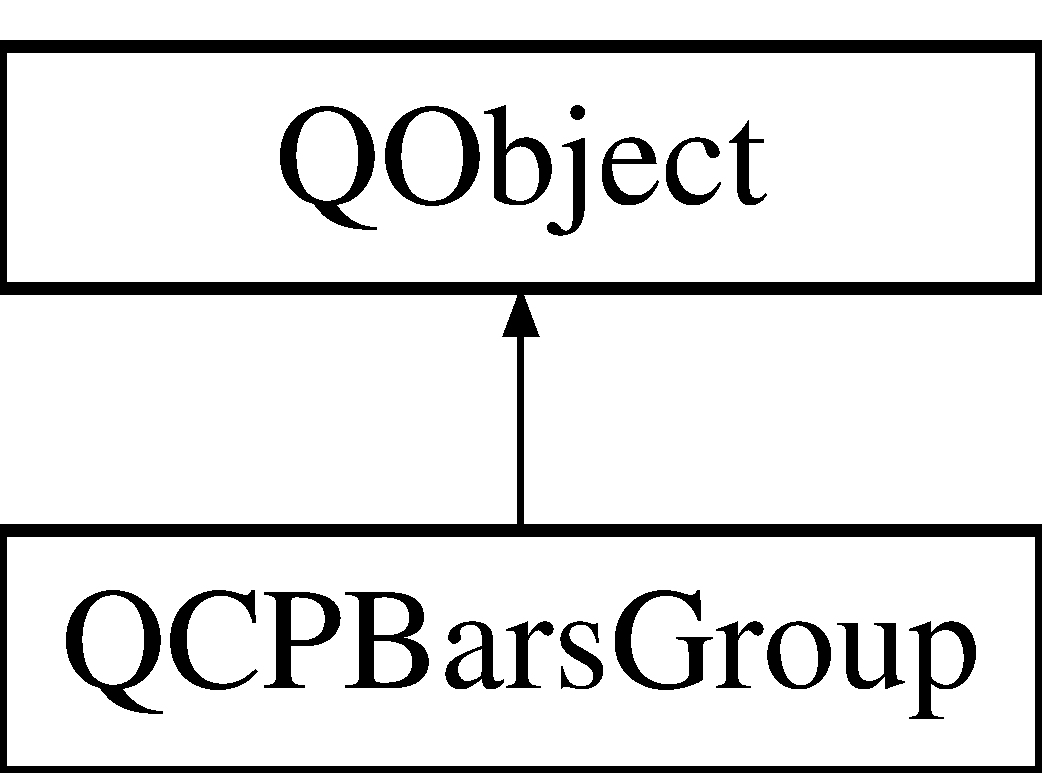
\includegraphics[height=2.000000cm]{class_q_c_p_bars_group}
\end{center}
\end{figure}
\subsection*{Public Types}
\begin{DoxyCompactItemize}
\item 
enum \hyperlink{class_q_c_p_bars_group_a4c0521120a97e60bbca37677a37075b6}{Spacing\+Type} \{ \hyperlink{class_q_c_p_bars_group_a4c0521120a97e60bbca37677a37075b6ab53fa3efaf14867dd0f14d41d64e42ac}{st\+Absolute}, 
\hyperlink{class_q_c_p_bars_group_a4c0521120a97e60bbca37677a37075b6ae94b05c27bc985dcdd8b1e1b7f163d26}{st\+Axis\+Rect\+Ratio}, 
\hyperlink{class_q_c_p_bars_group_a4c0521120a97e60bbca37677a37075b6ad369cee6287e0a86e8c2b643a3168c54}{st\+Plot\+Coords}
 \}
\end{DoxyCompactItemize}
\subsection*{Public Member Functions}
\begin{DoxyCompactItemize}
\item 
\hyperlink{class_q_c_p_bars_group_aa4e043b9a22c6c5ea0f93740aca063e1}{Q\+C\+P\+Bars\+Group} (\hyperlink{class_q_custom_plot}{Q\+Custom\+Plot} $\ast$parent\+Plot)
\item 
\hypertarget{class_q_c_p_bars_group_a894a77c45325aad2e742d936bc1f8aea}{}\label{class_q_c_p_bars_group_a894a77c45325aad2e742d936bc1f8aea} 
\hyperlink{class_q_c_p_bars_group_a4c0521120a97e60bbca37677a37075b6}{Spacing\+Type} {\bfseries spacing\+Type} () const
\item 
\hypertarget{class_q_c_p_bars_group_a314d09aeb2ad209518b9183ca7ffe662}{}\label{class_q_c_p_bars_group_a314d09aeb2ad209518b9183ca7ffe662} 
double {\bfseries spacing} () const
\item 
void \hyperlink{class_q_c_p_bars_group_a2c7e2d61b10594a4555b615e1fcaf49e}{set\+Spacing\+Type} (\hyperlink{class_q_c_p_bars_group_a4c0521120a97e60bbca37677a37075b6}{Spacing\+Type} spacing\+Type)
\item 
void \hyperlink{class_q_c_p_bars_group_aa553d327479d72a0c3dafcc724a190e2}{set\+Spacing} (double spacing)
\item 
Q\+List$<$ \hyperlink{class_q_c_p_bars}{Q\+C\+P\+Bars} $\ast$ $>$ \hyperlink{class_q_c_p_bars_group_a6e4f4e86abbec6a9342f204ef82abef8}{bars} () const
\item 
\hyperlink{class_q_c_p_bars}{Q\+C\+P\+Bars} $\ast$ \hyperlink{class_q_c_p_bars_group_a0754d659a020aa7fddfe81e657ce2d92}{bars} (int index) const
\item 
int \hyperlink{class_q_c_p_bars_group_a3780ec77919cb00840207ec7a0f00dd5}{size} () const
\item 
bool \hyperlink{class_q_c_p_bars_group_aac959e79e852e8ef9aea6e0449ad000a}{is\+Empty} () const
\item 
void \hyperlink{class_q_c_p_bars_group_a3ddf23928c6cd89530bd34ab7ba7b177}{clear} ()
\item 
bool \hyperlink{class_q_c_p_bars_group_ae26da07a23553052a178fb3fae90d0dc}{contains} (\hyperlink{class_q_c_p_bars}{Q\+C\+P\+Bars} $\ast$\hyperlink{class_q_c_p_bars_group_a6e4f4e86abbec6a9342f204ef82abef8}{bars}) const
\item 
void \hyperlink{class_q_c_p_bars_group_a809ed63cc4ff7cd5b0b8c96b470163d3}{append} (\hyperlink{class_q_c_p_bars}{Q\+C\+P\+Bars} $\ast$\hyperlink{class_q_c_p_bars_group_a6e4f4e86abbec6a9342f204ef82abef8}{bars})
\item 
void \hyperlink{class_q_c_p_bars_group_a309a5f7233db189f3ea9c2d04ece6c13}{insert} (int i, \hyperlink{class_q_c_p_bars}{Q\+C\+P\+Bars} $\ast$\hyperlink{class_q_c_p_bars_group_a6e4f4e86abbec6a9342f204ef82abef8}{bars})
\item 
void \hyperlink{class_q_c_p_bars_group_a215e28a5944f1159013a0e19169220e7}{remove} (\hyperlink{class_q_c_p_bars}{Q\+C\+P\+Bars} $\ast$\hyperlink{class_q_c_p_bars_group_a6e4f4e86abbec6a9342f204ef82abef8}{bars})
\end{DoxyCompactItemize}
\subsection*{Protected Member Functions}
\begin{DoxyCompactItemize}
\item 
\hypertarget{class_q_c_p_bars_group_a7b00514f19ad58d0bb3fd5246a67fae2}{}\label{class_q_c_p_bars_group_a7b00514f19ad58d0bb3fd5246a67fae2} 
void {\bfseries register\+Bars} (\hyperlink{class_q_c_p_bars}{Q\+C\+P\+Bars} $\ast$\hyperlink{class_q_c_p_bars_group_a6e4f4e86abbec6a9342f204ef82abef8}{bars})
\item 
\hypertarget{class_q_c_p_bars_group_ac7073cdd7b1a40c6cb4b5f908145f8c4}{}\label{class_q_c_p_bars_group_ac7073cdd7b1a40c6cb4b5f908145f8c4} 
void {\bfseries unregister\+Bars} (\hyperlink{class_q_c_p_bars}{Q\+C\+P\+Bars} $\ast$\hyperlink{class_q_c_p_bars_group_a6e4f4e86abbec6a9342f204ef82abef8}{bars})
\item 
\hypertarget{class_q_c_p_bars_group_a8e2ca6002e7bab49670144d048a2bcc9}{}\label{class_q_c_p_bars_group_a8e2ca6002e7bab49670144d048a2bcc9} 
double {\bfseries key\+Pixel\+Offset} (const \hyperlink{class_q_c_p_bars}{Q\+C\+P\+Bars} $\ast$\hyperlink{class_q_c_p_bars_group_a6e4f4e86abbec6a9342f204ef82abef8}{bars}, double key\+Coord)
\item 
\hypertarget{class_q_c_p_bars_group_a0beccd41bc3841a4c5b284823bc7d2de}{}\label{class_q_c_p_bars_group_a0beccd41bc3841a4c5b284823bc7d2de} 
double {\bfseries get\+Pixel\+Spacing} (const \hyperlink{class_q_c_p_bars}{Q\+C\+P\+Bars} $\ast$\hyperlink{class_q_c_p_bars_group_a6e4f4e86abbec6a9342f204ef82abef8}{bars}, double key\+Coord)
\end{DoxyCompactItemize}
\subsection*{Protected Attributes}
\begin{DoxyCompactItemize}
\item 
\hypertarget{class_q_c_p_bars_group_a973d408cfbf88db95115aec71877f9e7}{}\label{class_q_c_p_bars_group_a973d408cfbf88db95115aec71877f9e7} 
\hyperlink{class_q_custom_plot}{Q\+Custom\+Plot} $\ast$ {\bfseries m\+Parent\+Plot}
\item 
\hypertarget{class_q_c_p_bars_group_a6794ee1a9c81864d627bff6a4b2d64ec}{}\label{class_q_c_p_bars_group_a6794ee1a9c81864d627bff6a4b2d64ec} 
\hyperlink{class_q_c_p_bars_group_a4c0521120a97e60bbca37677a37075b6}{Spacing\+Type} {\bfseries m\+Spacing\+Type}
\item 
\hypertarget{class_q_c_p_bars_group_a56471d7f548ca6141b7a5bf9629f7ece}{}\label{class_q_c_p_bars_group_a56471d7f548ca6141b7a5bf9629f7ece} 
double {\bfseries m\+Spacing}
\item 
\hypertarget{class_q_c_p_bars_group_affdb1e9233c277ff5a4c0a1121cf1fc0}{}\label{class_q_c_p_bars_group_affdb1e9233c277ff5a4c0a1121cf1fc0} 
Q\+List$<$ \hyperlink{class_q_c_p_bars}{Q\+C\+P\+Bars} $\ast$ $>$ {\bfseries m\+Bars}
\end{DoxyCompactItemize}
\subsection*{Friends}
\begin{DoxyCompactItemize}
\item 
\hypertarget{class_q_c_p_bars_group_a721b87c7cdb8e83a90d77fc8a22e7195}{}\label{class_q_c_p_bars_group_a721b87c7cdb8e83a90d77fc8a22e7195} 
class {\bfseries Q\+C\+P\+Bars}
\end{DoxyCompactItemize}


\subsection{Detailed Description}
Groups multiple \hyperlink{class_q_c_p_bars}{Q\+C\+P\+Bars} together so they appear side by side. 



When showing multiple \hyperlink{class_q_c_p_bars}{Q\+C\+P\+Bars} in one plot which have bars at identical keys, it may be desirable to have them appearing next to each other at each key. This is what adding the respective \hyperlink{class_q_c_p_bars}{Q\+C\+P\+Bars} plottables to a \hyperlink{class_q_c_p_bars_group}{Q\+C\+P\+Bars\+Group} achieves. (An alternative approach is to stack them on top of each other, see \hyperlink{class_q_c_p_bars_ac22e00a6a41509538c21b04f0a57318c}{Q\+C\+P\+Bars\+::move\+Above}.)\hypertarget{class_q_c_p_bars_group_qcpbarsgroup-usage}{}\subsection{Usage}\label{class_q_c_p_bars_group_qcpbarsgroup-usage}
To add a \hyperlink{class_q_c_p_bars}{Q\+C\+P\+Bars} plottable to the group, create a new group and then add the respective bars intances\+: 
\begin{DoxyCodeInclude}
\end{DoxyCodeInclude}
Alternatively to appending to the group like shown above, you can also set the group on the \hyperlink{class_q_c_p_bars}{Q\+C\+P\+Bars} plottable via \hyperlink{class_q_c_p_bars_aedd1709061f0b307c47ddb45e172ef9a}{Q\+C\+P\+Bars\+::set\+Bars\+Group}.

The spacing between the bars can be configured via \hyperlink{class_q_c_p_bars_group_a2c7e2d61b10594a4555b615e1fcaf49e}{set\+Spacing\+Type} and \hyperlink{class_q_c_p_bars_group_aa553d327479d72a0c3dafcc724a190e2}{set\+Spacing}. The bars in this group appear in the plot in the order they were appended. To insert a bars plottable at a certain index position, or to reposition a bars plottable which is already in the group, use \hyperlink{class_q_c_p_bars_group_a309a5f7233db189f3ea9c2d04ece6c13}{insert}.

To remove specific bars from the group, use either \hyperlink{class_q_c_p_bars_group_a215e28a5944f1159013a0e19169220e7}{remove} or call \hyperlink{class_q_c_p_bars_aedd1709061f0b307c47ddb45e172ef9a}{Q\+C\+P\+Bars\+:\+:set\+Bars\+Group(0)} on the respective bars plottable.

To clear the entire group, call \hyperlink{class_q_c_p_bars_group_a3ddf23928c6cd89530bd34ab7ba7b177}{clear}, or simply delete the group.\hypertarget{class_q_c_p_bars_group_qcpbarsgroup-example}{}\subsection{Example}\label{class_q_c_p_bars_group_qcpbarsgroup-example}
The image above is generated with the following code\+: 
\begin{DoxyCodeInclude}
\end{DoxyCodeInclude}


\subsection{Member Enumeration Documentation}
\hypertarget{class_q_c_p_bars_group_a4c0521120a97e60bbca37677a37075b6}{}\label{class_q_c_p_bars_group_a4c0521120a97e60bbca37677a37075b6} 
\index{Q\+C\+P\+Bars\+Group@{Q\+C\+P\+Bars\+Group}!Spacing\+Type@{Spacing\+Type}}
\index{Spacing\+Type@{Spacing\+Type}!Q\+C\+P\+Bars\+Group@{Q\+C\+P\+Bars\+Group}}
\subsubsection{\texorpdfstring{Spacing\+Type}{SpacingType}}
{\footnotesize\ttfamily enum \hyperlink{class_q_c_p_bars_group_a4c0521120a97e60bbca37677a37075b6}{Q\+C\+P\+Bars\+Group\+::\+Spacing\+Type}}

Defines the ways the spacing between bars in the group can be specified. Thus it defines what the number passed to \hyperlink{class_q_c_p_bars_group_aa553d327479d72a0c3dafcc724a190e2}{set\+Spacing} actually means.

\begin{DoxySeeAlso}{See also}
\hyperlink{class_q_c_p_bars_group_a2c7e2d61b10594a4555b615e1fcaf49e}{set\+Spacing\+Type}, \hyperlink{class_q_c_p_bars_group_aa553d327479d72a0c3dafcc724a190e2}{set\+Spacing} 
\end{DoxySeeAlso}
\begin{DoxyEnumFields}{Enumerator}
\raisebox{\heightof{T}}[0pt][0pt]{\index{st\+Absolute@{st\+Absolute}!Q\+C\+P\+Bars\+Group@{Q\+C\+P\+Bars\+Group}}\index{Q\+C\+P\+Bars\+Group@{Q\+C\+P\+Bars\+Group}!st\+Absolute@{st\+Absolute}}}\hypertarget{class_q_c_p_bars_group_a4c0521120a97e60bbca37677a37075b6ab53fa3efaf14867dd0f14d41d64e42ac}{}\label{class_q_c_p_bars_group_a4c0521120a97e60bbca37677a37075b6ab53fa3efaf14867dd0f14d41d64e42ac} 
st\+Absolute&Bar spacing is in absolute pixels. \\
\hline

\raisebox{\heightof{T}}[0pt][0pt]{\index{st\+Axis\+Rect\+Ratio@{st\+Axis\+Rect\+Ratio}!Q\+C\+P\+Bars\+Group@{Q\+C\+P\+Bars\+Group}}\index{Q\+C\+P\+Bars\+Group@{Q\+C\+P\+Bars\+Group}!st\+Axis\+Rect\+Ratio@{st\+Axis\+Rect\+Ratio}}}\hypertarget{class_q_c_p_bars_group_a4c0521120a97e60bbca37677a37075b6ae94b05c27bc985dcdd8b1e1b7f163d26}{}\label{class_q_c_p_bars_group_a4c0521120a97e60bbca37677a37075b6ae94b05c27bc985dcdd8b1e1b7f163d26} 
st\+Axis\+Rect\+Ratio&Bar spacing is given by a fraction of the axis rect size. \\
\hline

\raisebox{\heightof{T}}[0pt][0pt]{\index{st\+Plot\+Coords@{st\+Plot\+Coords}!Q\+C\+P\+Bars\+Group@{Q\+C\+P\+Bars\+Group}}\index{Q\+C\+P\+Bars\+Group@{Q\+C\+P\+Bars\+Group}!st\+Plot\+Coords@{st\+Plot\+Coords}}}\hypertarget{class_q_c_p_bars_group_a4c0521120a97e60bbca37677a37075b6ad369cee6287e0a86e8c2b643a3168c54}{}\label{class_q_c_p_bars_group_a4c0521120a97e60bbca37677a37075b6ad369cee6287e0a86e8c2b643a3168c54} 
st\+Plot\+Coords&Bar spacing is in key coordinates and thus scales with the key axis range. \\
\hline

\end{DoxyEnumFields}


\subsection{Constructor \& Destructor Documentation}
\hypertarget{class_q_c_p_bars_group_aa4e043b9a22c6c5ea0f93740aca063e1}{}\label{class_q_c_p_bars_group_aa4e043b9a22c6c5ea0f93740aca063e1} 
\index{Q\+C\+P\+Bars\+Group@{Q\+C\+P\+Bars\+Group}!Q\+C\+P\+Bars\+Group@{Q\+C\+P\+Bars\+Group}}
\index{Q\+C\+P\+Bars\+Group@{Q\+C\+P\+Bars\+Group}!Q\+C\+P\+Bars\+Group@{Q\+C\+P\+Bars\+Group}}
\subsubsection{\texorpdfstring{Q\+C\+P\+Bars\+Group()}{QCPBarsGroup()}}
{\footnotesize\ttfamily Q\+C\+P\+Bars\+Group\+::\+Q\+C\+P\+Bars\+Group (\begin{DoxyParamCaption}\item[{\hyperlink{class_q_custom_plot}{Q\+Custom\+Plot} $\ast$}]{parent\+Plot }\end{DoxyParamCaption})}

Constructs a new bars group for the specified \hyperlink{class_q_custom_plot}{Q\+Custom\+Plot} instance. 

\subsection{Member Function Documentation}
\hypertarget{class_q_c_p_bars_group_a809ed63cc4ff7cd5b0b8c96b470163d3}{}\label{class_q_c_p_bars_group_a809ed63cc4ff7cd5b0b8c96b470163d3} 
\index{Q\+C\+P\+Bars\+Group@{Q\+C\+P\+Bars\+Group}!append@{append}}
\index{append@{append}!Q\+C\+P\+Bars\+Group@{Q\+C\+P\+Bars\+Group}}
\subsubsection{\texorpdfstring{append()}{append()}}
{\footnotesize\ttfamily void Q\+C\+P\+Bars\+Group\+::append (\begin{DoxyParamCaption}\item[{\hyperlink{class_q_c_p_bars}{Q\+C\+P\+Bars} $\ast$}]{bars }\end{DoxyParamCaption})}

Adds the specified {\itshape bars} plottable to this group. Alternatively, you can also use \hyperlink{class_q_c_p_bars_aedd1709061f0b307c47ddb45e172ef9a}{Q\+C\+P\+Bars\+::set\+Bars\+Group} on the {\itshape bars} instance.

\begin{DoxySeeAlso}{See also}
\hyperlink{class_q_c_p_bars_group_a309a5f7233db189f3ea9c2d04ece6c13}{insert}, \hyperlink{class_q_c_p_bars_group_a215e28a5944f1159013a0e19169220e7}{remove} 
\end{DoxySeeAlso}
\hypertarget{class_q_c_p_bars_group_a6e4f4e86abbec6a9342f204ef82abef8}{}\label{class_q_c_p_bars_group_a6e4f4e86abbec6a9342f204ef82abef8} 
\index{Q\+C\+P\+Bars\+Group@{Q\+C\+P\+Bars\+Group}!bars@{bars}}
\index{bars@{bars}!Q\+C\+P\+Bars\+Group@{Q\+C\+P\+Bars\+Group}}
\subsubsection{\texorpdfstring{bars()}{bars()}\hspace{0.1cm}{\footnotesize\ttfamily [1/2]}}
{\footnotesize\ttfamily Q\+List$<$ \hyperlink{class_q_c_p_bars}{Q\+C\+P\+Bars} $\ast$ $>$ Q\+C\+P\+Bars\+Group\+::bars (\begin{DoxyParamCaption}{ }\end{DoxyParamCaption}) const\hspace{0.3cm}{\ttfamily [inline]}}

Returns all bars currently in this group.

\begin{DoxySeeAlso}{See also}
bars(int index) 
\end{DoxySeeAlso}
\hypertarget{class_q_c_p_bars_group_a0754d659a020aa7fddfe81e657ce2d92}{}\label{class_q_c_p_bars_group_a0754d659a020aa7fddfe81e657ce2d92} 
\index{Q\+C\+P\+Bars\+Group@{Q\+C\+P\+Bars\+Group}!bars@{bars}}
\index{bars@{bars}!Q\+C\+P\+Bars\+Group@{Q\+C\+P\+Bars\+Group}}
\subsubsection{\texorpdfstring{bars()}{bars()}\hspace{0.1cm}{\footnotesize\ttfamily [2/2]}}
{\footnotesize\ttfamily \hyperlink{class_q_c_p_bars}{Q\+C\+P\+Bars} $\ast$ Q\+C\+P\+Bars\+Group\+::bars (\begin{DoxyParamCaption}\item[{int}]{index }\end{DoxyParamCaption}) const}

Returns the \hyperlink{class_q_c_p_bars}{Q\+C\+P\+Bars} instance with the specified {\itshape index} in this group. If no such \hyperlink{class_q_c_p_bars}{Q\+C\+P\+Bars} exists, returns 0.

\begin{DoxySeeAlso}{See also}
\hyperlink{class_q_c_p_bars_group_a6e4f4e86abbec6a9342f204ef82abef8}{bars()}, \hyperlink{class_q_c_p_bars_group_a3780ec77919cb00840207ec7a0f00dd5}{size} 
\end{DoxySeeAlso}
\hypertarget{class_q_c_p_bars_group_a3ddf23928c6cd89530bd34ab7ba7b177}{}\label{class_q_c_p_bars_group_a3ddf23928c6cd89530bd34ab7ba7b177} 
\index{Q\+C\+P\+Bars\+Group@{Q\+C\+P\+Bars\+Group}!clear@{clear}}
\index{clear@{clear}!Q\+C\+P\+Bars\+Group@{Q\+C\+P\+Bars\+Group}}
\subsubsection{\texorpdfstring{clear()}{clear()}}
{\footnotesize\ttfamily void Q\+C\+P\+Bars\+Group\+::clear (\begin{DoxyParamCaption}{ }\end{DoxyParamCaption})}

Removes all \hyperlink{class_q_c_p_bars}{Q\+C\+P\+Bars} plottables from this group.

\begin{DoxySeeAlso}{See also}
\hyperlink{class_q_c_p_bars_group_aac959e79e852e8ef9aea6e0449ad000a}{is\+Empty} 
\end{DoxySeeAlso}
\hypertarget{class_q_c_p_bars_group_ae26da07a23553052a178fb3fae90d0dc}{}\label{class_q_c_p_bars_group_ae26da07a23553052a178fb3fae90d0dc} 
\index{Q\+C\+P\+Bars\+Group@{Q\+C\+P\+Bars\+Group}!contains@{contains}}
\index{contains@{contains}!Q\+C\+P\+Bars\+Group@{Q\+C\+P\+Bars\+Group}}
\subsubsection{\texorpdfstring{contains()}{contains()}}
{\footnotesize\ttfamily bool Q\+C\+P\+Bars\+Group\+::contains (\begin{DoxyParamCaption}\item[{\hyperlink{class_q_c_p_bars}{Q\+C\+P\+Bars} $\ast$}]{bars }\end{DoxyParamCaption}) const\hspace{0.3cm}{\ttfamily [inline]}}

Returns whether the specified {\itshape bars} plottable is part of this group. \hypertarget{class_q_c_p_bars_group_a309a5f7233db189f3ea9c2d04ece6c13}{}\label{class_q_c_p_bars_group_a309a5f7233db189f3ea9c2d04ece6c13} 
\index{Q\+C\+P\+Bars\+Group@{Q\+C\+P\+Bars\+Group}!insert@{insert}}
\index{insert@{insert}!Q\+C\+P\+Bars\+Group@{Q\+C\+P\+Bars\+Group}}
\subsubsection{\texorpdfstring{insert()}{insert()}}
{\footnotesize\ttfamily void Q\+C\+P\+Bars\+Group\+::insert (\begin{DoxyParamCaption}\item[{int}]{i,  }\item[{\hyperlink{class_q_c_p_bars}{Q\+C\+P\+Bars} $\ast$}]{bars }\end{DoxyParamCaption})}

Inserts the specified {\itshape bars} plottable into this group at the specified index position {\itshape i}. This gives you full control over the ordering of the bars.

{\itshape bars} may already be part of this group. In that case, {\itshape bars} is just moved to the new index position.

\begin{DoxySeeAlso}{See also}
\hyperlink{class_q_c_p_bars_group_a809ed63cc4ff7cd5b0b8c96b470163d3}{append}, \hyperlink{class_q_c_p_bars_group_a215e28a5944f1159013a0e19169220e7}{remove} 
\end{DoxySeeAlso}
\hypertarget{class_q_c_p_bars_group_aac959e79e852e8ef9aea6e0449ad000a}{}\label{class_q_c_p_bars_group_aac959e79e852e8ef9aea6e0449ad000a} 
\index{Q\+C\+P\+Bars\+Group@{Q\+C\+P\+Bars\+Group}!is\+Empty@{is\+Empty}}
\index{is\+Empty@{is\+Empty}!Q\+C\+P\+Bars\+Group@{Q\+C\+P\+Bars\+Group}}
\subsubsection{\texorpdfstring{is\+Empty()}{isEmpty()}}
{\footnotesize\ttfamily bool Q\+C\+P\+Bars\+Group\+::is\+Empty (\begin{DoxyParamCaption}{ }\end{DoxyParamCaption}) const\hspace{0.3cm}{\ttfamily [inline]}}

Returns whether this bars group is empty.

\begin{DoxySeeAlso}{See also}
\hyperlink{class_q_c_p_bars_group_a3780ec77919cb00840207ec7a0f00dd5}{size} 
\end{DoxySeeAlso}
\hypertarget{class_q_c_p_bars_group_a215e28a5944f1159013a0e19169220e7}{}\label{class_q_c_p_bars_group_a215e28a5944f1159013a0e19169220e7} 
\index{Q\+C\+P\+Bars\+Group@{Q\+C\+P\+Bars\+Group}!remove@{remove}}
\index{remove@{remove}!Q\+C\+P\+Bars\+Group@{Q\+C\+P\+Bars\+Group}}
\subsubsection{\texorpdfstring{remove()}{remove()}}
{\footnotesize\ttfamily void Q\+C\+P\+Bars\+Group\+::remove (\begin{DoxyParamCaption}\item[{\hyperlink{class_q_c_p_bars}{Q\+C\+P\+Bars} $\ast$}]{bars }\end{DoxyParamCaption})}

Removes the specified {\itshape bars} plottable from this group.

\begin{DoxySeeAlso}{See also}
\hyperlink{class_q_c_p_bars_group_ae26da07a23553052a178fb3fae90d0dc}{contains}, \hyperlink{class_q_c_p_bars_group_a3ddf23928c6cd89530bd34ab7ba7b177}{clear} 
\end{DoxySeeAlso}
\hypertarget{class_q_c_p_bars_group_aa553d327479d72a0c3dafcc724a190e2}{}\label{class_q_c_p_bars_group_aa553d327479d72a0c3dafcc724a190e2} 
\index{Q\+C\+P\+Bars\+Group@{Q\+C\+P\+Bars\+Group}!set\+Spacing@{set\+Spacing}}
\index{set\+Spacing@{set\+Spacing}!Q\+C\+P\+Bars\+Group@{Q\+C\+P\+Bars\+Group}}
\subsubsection{\texorpdfstring{set\+Spacing()}{setSpacing()}}
{\footnotesize\ttfamily void Q\+C\+P\+Bars\+Group\+::set\+Spacing (\begin{DoxyParamCaption}\item[{double}]{spacing }\end{DoxyParamCaption})}

Sets the spacing between adjacent bars. What the number passed as {\itshape spacing} actually means, is defined by the current \hyperlink{class_q_c_p_bars_group_a4c0521120a97e60bbca37677a37075b6}{Spacing\+Type}, which can be set with \hyperlink{class_q_c_p_bars_group_a2c7e2d61b10594a4555b615e1fcaf49e}{set\+Spacing\+Type}.

\begin{DoxySeeAlso}{See also}
\hyperlink{class_q_c_p_bars_group_a2c7e2d61b10594a4555b615e1fcaf49e}{set\+Spacing\+Type} 
\end{DoxySeeAlso}
\hypertarget{class_q_c_p_bars_group_a2c7e2d61b10594a4555b615e1fcaf49e}{}\label{class_q_c_p_bars_group_a2c7e2d61b10594a4555b615e1fcaf49e} 
\index{Q\+C\+P\+Bars\+Group@{Q\+C\+P\+Bars\+Group}!set\+Spacing\+Type@{set\+Spacing\+Type}}
\index{set\+Spacing\+Type@{set\+Spacing\+Type}!Q\+C\+P\+Bars\+Group@{Q\+C\+P\+Bars\+Group}}
\subsubsection{\texorpdfstring{set\+Spacing\+Type()}{setSpacingType()}}
{\footnotesize\ttfamily void Q\+C\+P\+Bars\+Group\+::set\+Spacing\+Type (\begin{DoxyParamCaption}\item[{\hyperlink{class_q_c_p_bars_group_a4c0521120a97e60bbca37677a37075b6}{Spacing\+Type}}]{spacing\+Type }\end{DoxyParamCaption})}

Sets how the spacing between adjacent bars is interpreted. See \hyperlink{class_q_c_p_bars_group_a4c0521120a97e60bbca37677a37075b6}{Spacing\+Type}.

The actual spacing can then be specified with \hyperlink{class_q_c_p_bars_group_aa553d327479d72a0c3dafcc724a190e2}{set\+Spacing}.

\begin{DoxySeeAlso}{See also}
\hyperlink{class_q_c_p_bars_group_aa553d327479d72a0c3dafcc724a190e2}{set\+Spacing} 
\end{DoxySeeAlso}
\hypertarget{class_q_c_p_bars_group_a3780ec77919cb00840207ec7a0f00dd5}{}\label{class_q_c_p_bars_group_a3780ec77919cb00840207ec7a0f00dd5} 
\index{Q\+C\+P\+Bars\+Group@{Q\+C\+P\+Bars\+Group}!size@{size}}
\index{size@{size}!Q\+C\+P\+Bars\+Group@{Q\+C\+P\+Bars\+Group}}
\subsubsection{\texorpdfstring{size()}{size()}}
{\footnotesize\ttfamily int Q\+C\+P\+Bars\+Group\+::size (\begin{DoxyParamCaption}{ }\end{DoxyParamCaption}) const\hspace{0.3cm}{\ttfamily [inline]}}

Returns the number of \hyperlink{class_q_c_p_bars}{Q\+C\+P\+Bars} plottables that are part of this group. 

The documentation for this class was generated from the following files\+:\begin{DoxyCompactItemize}
\item 
C\+:/\+Users/\+Jesse Jutson/\+Documents/\+Git\+Hub/\+F\+E\+S\+S\+G\+U\+I/\+F\+E\+S\+S-\/\+G\+U\+I/\hyperlink{qcustomplot_8h}{qcustomplot.\+h}\item 
C\+:/\+Users/\+Jesse Jutson/\+Documents/\+Git\+Hub/\+F\+E\+S\+S\+G\+U\+I/\+F\+E\+S\+S-\/\+G\+U\+I/\hyperlink{qcustomplot_8cpp}{qcustomplot.\+cpp}\end{DoxyCompactItemize}

\hypertarget{class_q_c_p_color_gradient}{}\section{Q\+C\+P\+Color\+Gradient Class Reference}
\label{class_q_c_p_color_gradient}\index{Q\+C\+P\+Color\+Gradient@{Q\+C\+P\+Color\+Gradient}}


Defines a color gradient for use with e.\+g. \hyperlink{class_q_c_p_color_map}{Q\+C\+P\+Color\+Map}.  


\subsection*{Public Types}
\begin{DoxyCompactItemize}
\item 
enum \hyperlink{class_q_c_p_color_gradient_ac5dca17cc24336e6ca176610e7f77fc1}{Color\+Interpolation} \{ \hyperlink{class_q_c_p_color_gradient_ac5dca17cc24336e6ca176610e7f77fc1a5e30f725c9cfe93999e268a9f92afbe7}{ci\+R\+GB}, 
\hyperlink{class_q_c_p_color_gradient_ac5dca17cc24336e6ca176610e7f77fc1af14ae62fcae11ecc07234eeaec5856cb}{ci\+H\+SV}
 \}
\item 
enum \hyperlink{class_q_c_p_color_gradient_aed6569828fee337023670272910c9072}{Gradient\+Preset} \{ \newline
\hyperlink{class_q_c_p_color_gradient_aed6569828fee337023670272910c9072add11ae369a86f3b1b6205ec72e5021fb}{gp\+Grayscale}, 
\hyperlink{class_q_c_p_color_gradient_aed6569828fee337023670272910c9072a4f42e534cf6cff5a29a5388094d099b5}{gp\+Hot}, 
\hyperlink{class_q_c_p_color_gradient_aed6569828fee337023670272910c9072aec8c001f62c0d5cb853db5fd85309557}{gp\+Cold}, 
\hyperlink{class_q_c_p_color_gradient_aed6569828fee337023670272910c9072a1bb89351b6def7d220973443fe059c62}{gp\+Night}, 
\newline
\hyperlink{class_q_c_p_color_gradient_aed6569828fee337023670272910c9072a9e72663bf6b94b65945f7843f24e0721}{gp\+Candy}, 
\hyperlink{class_q_c_p_color_gradient_aed6569828fee337023670272910c9072a382f0b07cec1a59d8a533438aea815d2}{gp\+Geography}, 
\hyperlink{class_q_c_p_color_gradient_aed6569828fee337023670272910c9072a4297f4f9e212a819cd65e8e34567182b}{gp\+Ion}, 
\hyperlink{class_q_c_p_color_gradient_aed6569828fee337023670272910c9072af1676b129f9f458ace453f280c731cf7}{gp\+Thermal}, 
\newline
\hyperlink{class_q_c_p_color_gradient_aed6569828fee337023670272910c9072ab7414ce4e36dc3e82e0132a7f0f41b52}{gp\+Polar}, 
\hyperlink{class_q_c_p_color_gradient_aed6569828fee337023670272910c9072ad63adc100ef46f6b4a8a6deacec4642f}{gp\+Spectrum}, 
\hyperlink{class_q_c_p_color_gradient_aed6569828fee337023670272910c9072a5f8a9e67b64c17ddfe4f069fe2b9fb02}{gp\+Jet}, 
\hyperlink{class_q_c_p_color_gradient_aed6569828fee337023670272910c9072a30efe58407acfb67939032f70213a130}{gp\+Hues}
 \}
\end{DoxyCompactItemize}
\subsection*{Public Member Functions}
\begin{DoxyCompactItemize}
\item 
\hyperlink{class_q_c_p_color_gradient_a546e44df5fa1846400a582c041361c85}{Q\+C\+P\+Color\+Gradient} (\hyperlink{class_q_c_p_color_gradient_aed6569828fee337023670272910c9072}{Gradient\+Preset} preset=\hyperlink{class_q_c_p_color_gradient_aed6569828fee337023670272910c9072aec8c001f62c0d5cb853db5fd85309557}{gp\+Cold})
\item 
\hypertarget{class_q_c_p_color_gradient_a7f3478c33c59aa3c03b9ea1f809877fa}{}\label{class_q_c_p_color_gradient_a7f3478c33c59aa3c03b9ea1f809877fa} 
bool {\bfseries operator==} (const \hyperlink{class_q_c_p_color_gradient}{Q\+C\+P\+Color\+Gradient} \&other) const
\item 
\hypertarget{class_q_c_p_color_gradient_ad26a10e3beaef4fc6f2553d1a9756087}{}\label{class_q_c_p_color_gradient_ad26a10e3beaef4fc6f2553d1a9756087} 
bool {\bfseries operator!=} (const \hyperlink{class_q_c_p_color_gradient}{Q\+C\+P\+Color\+Gradient} \&other) const
\item 
\hypertarget{class_q_c_p_color_gradient_ac4b9d7034fc3b6c76318b05075367090}{}\label{class_q_c_p_color_gradient_ac4b9d7034fc3b6c76318b05075367090} 
int {\bfseries level\+Count} () const
\item 
\hypertarget{class_q_c_p_color_gradient_aaab19729e921682401044ac8e518ff02}{}\label{class_q_c_p_color_gradient_aaab19729e921682401044ac8e518ff02} 
Q\+Map$<$ double, Q\+Color $>$ {\bfseries color\+Stops} () const
\item 
\hypertarget{class_q_c_p_color_gradient_abad5002858db8cf75ecb045200881de6}{}\label{class_q_c_p_color_gradient_abad5002858db8cf75ecb045200881de6} 
\hyperlink{class_q_c_p_color_gradient_ac5dca17cc24336e6ca176610e7f77fc1}{Color\+Interpolation} {\bfseries color\+Interpolation} () const
\item 
\hypertarget{class_q_c_p_color_gradient_a22a1d2b17f203caf0dcec833507fb9e0}{}\label{class_q_c_p_color_gradient_a22a1d2b17f203caf0dcec833507fb9e0} 
bool {\bfseries periodic} () const
\item 
void \hyperlink{class_q_c_p_color_gradient_a18da587eb4f7fc788ea28ba15b6a12de}{set\+Level\+Count} (int n)
\item 
void \hyperlink{class_q_c_p_color_gradient_a724e828aa6f0ba5011a9392477c35d3a}{set\+Color\+Stops} (const Q\+Map$<$ double, Q\+Color $>$ \&color\+Stops)
\item 
void \hyperlink{class_q_c_p_color_gradient_a3b48be5e78079db1bb2a1188a4c3390e}{set\+Color\+Stop\+At} (double position, const Q\+Color \&color)
\item 
void \hyperlink{class_q_c_p_color_gradient_aa13fda86406e1d896a465a409ae63b38}{set\+Color\+Interpolation} (\hyperlink{class_q_c_p_color_gradient_ac5dca17cc24336e6ca176610e7f77fc1}{Color\+Interpolation} interpolation)
\item 
void \hyperlink{class_q_c_p_color_gradient_a39d6448155fc00a219f239220d14bb39}{set\+Periodic} (bool enabled)
\item 
void \hyperlink{class_q_c_p_color_gradient_aaf423ceb943e177b0ed2c48c811d83dc}{colorize} (const double $\ast$data, const \hyperlink{class_q_c_p_range}{Q\+C\+P\+Range} \&range, Q\+Rgb $\ast$scan\+Line, int n, int data\+Index\+Factor=1, bool logarithmic=false)
\item 
\hypertarget{class_q_c_p_color_gradient_a0599545c859268b025d2060dea741cea}{}\label{class_q_c_p_color_gradient_a0599545c859268b025d2060dea741cea} 
Q\+Rgb {\bfseries color} (double position, const \hyperlink{class_q_c_p_range}{Q\+C\+P\+Range} \&range, bool logarithmic=false)
\item 
void \hyperlink{class_q_c_p_color_gradient_aa0aeec1528241728b9671bf8e60b1622}{load\+Preset} (\hyperlink{class_q_c_p_color_gradient_aed6569828fee337023670272910c9072}{Gradient\+Preset} preset)
\item 
void \hyperlink{class_q_c_p_color_gradient_a939213e85f0d1279519d555c5fcfb6ad}{clear\+Color\+Stops} ()
\item 
\hyperlink{class_q_c_p_color_gradient}{Q\+C\+P\+Color\+Gradient} \hyperlink{class_q_c_p_color_gradient_a9f72f501de429829ec446333316decda}{inverted} () const
\end{DoxyCompactItemize}
\subsection*{Protected Member Functions}
\begin{DoxyCompactItemize}
\item 
\hypertarget{class_q_c_p_color_gradient_a353f15ab3ab586eebf1f6b58c3e2707b}{}\label{class_q_c_p_color_gradient_a353f15ab3ab586eebf1f6b58c3e2707b} 
void {\bfseries update\+Color\+Buffer} ()
\end{DoxyCompactItemize}
\subsection*{Protected Attributes}
\begin{DoxyCompactItemize}
\item 
\hypertarget{class_q_c_p_color_gradient_a98fb68e359904b2c991fcae3e38a211a}{}\label{class_q_c_p_color_gradient_a98fb68e359904b2c991fcae3e38a211a} 
int {\bfseries m\+Level\+Count}
\item 
\hypertarget{class_q_c_p_color_gradient_a9e11a2b0974ef289d12c324822bc3a3e}{}\label{class_q_c_p_color_gradient_a9e11a2b0974ef289d12c324822bc3a3e} 
Q\+Map$<$ double, Q\+Color $>$ {\bfseries m\+Color\+Stops}
\item 
\hypertarget{class_q_c_p_color_gradient_a028cef73d863800a9ee93ffd641cce01}{}\label{class_q_c_p_color_gradient_a028cef73d863800a9ee93ffd641cce01} 
\hyperlink{class_q_c_p_color_gradient_ac5dca17cc24336e6ca176610e7f77fc1}{Color\+Interpolation} {\bfseries m\+Color\+Interpolation}
\item 
\hypertarget{class_q_c_p_color_gradient_a4b07deeb20ca1ee2d5ea7e01bf0420af}{}\label{class_q_c_p_color_gradient_a4b07deeb20ca1ee2d5ea7e01bf0420af} 
bool {\bfseries m\+Periodic}
\item 
\hypertarget{class_q_c_p_color_gradient_af8b5f0739faa5f8295154d47ce38ecff}{}\label{class_q_c_p_color_gradient_af8b5f0739faa5f8295154d47ce38ecff} 
Q\+Vector$<$ Q\+Rgb $>$ {\bfseries m\+Color\+Buffer}
\item 
\hypertarget{class_q_c_p_color_gradient_abacf55e11f67d6722a687af1bb2687bd}{}\label{class_q_c_p_color_gradient_abacf55e11f67d6722a687af1bb2687bd} 
bool {\bfseries m\+Color\+Buffer\+Invalidated}
\end{DoxyCompactItemize}


\subsection{Detailed Description}
Defines a color gradient for use with e.\+g. \hyperlink{class_q_c_p_color_map}{Q\+C\+P\+Color\+Map}. 

This class describes a color gradient which can be used to encode data with color. For example, \hyperlink{class_q_c_p_color_map}{Q\+C\+P\+Color\+Map} and \hyperlink{class_q_c_p_color_scale}{Q\+C\+P\+Color\+Scale} have \hyperlink{class_q_c_p_color_map_a7313c78360471cead3576341a2c50377}{set\+Gradient} methods which take an instance of this class. Colors are set with \hyperlink{class_q_c_p_color_gradient_a3b48be5e78079db1bb2a1188a4c3390e}{set\+Color\+Stop\+At(double position, const Q\+Color \&color)} with a {\itshape position} from 0 to 1. In between these defined color positions, the color will be interpolated linearly either in R\+GB or H\+SV space, see \hyperlink{class_q_c_p_color_gradient_aa13fda86406e1d896a465a409ae63b38}{set\+Color\+Interpolation}.

Alternatively, load one of the preset color gradients shown in the image below, with \hyperlink{class_q_c_p_color_gradient_aa0aeec1528241728b9671bf8e60b1622}{load\+Preset}, or by directly specifying the preset in the constructor.



The fact that the \hyperlink{class_q_c_p_color_gradient}{ructor} allows directly converting a \hyperlink{class_q_c_p_color_gradient_aed6569828fee337023670272910c9072}{Gradient\+Preset} to a \hyperlink{class_q_c_p_color_gradient}{Q\+C\+P\+Color\+Gradient}, you can also directly pass \hyperlink{class_q_c_p_color_gradient_aed6569828fee337023670272910c9072}{Gradient\+Preset} to all the {\itshape set\+Gradient} methods, e.\+g.\+: 
\begin{DoxyCodeInclude}
\end{DoxyCodeInclude}
 The total number of levels used in the gradient can be set with \hyperlink{class_q_c_p_color_gradient_a18da587eb4f7fc788ea28ba15b6a12de}{set\+Level\+Count}. Whether the color gradient shall be applied periodically (wrapping around) to data values that lie outside the data range specified on the plottable instance can be controlled with \hyperlink{class_q_c_p_color_gradient_a39d6448155fc00a219f239220d14bb39}{set\+Periodic}. 

\subsection{Member Enumeration Documentation}
\hypertarget{class_q_c_p_color_gradient_ac5dca17cc24336e6ca176610e7f77fc1}{}\label{class_q_c_p_color_gradient_ac5dca17cc24336e6ca176610e7f77fc1} 
\index{Q\+C\+P\+Color\+Gradient@{Q\+C\+P\+Color\+Gradient}!Color\+Interpolation@{Color\+Interpolation}}
\index{Color\+Interpolation@{Color\+Interpolation}!Q\+C\+P\+Color\+Gradient@{Q\+C\+P\+Color\+Gradient}}
\subsubsection{\texorpdfstring{Color\+Interpolation}{ColorInterpolation}}
{\footnotesize\ttfamily enum \hyperlink{class_q_c_p_color_gradient_ac5dca17cc24336e6ca176610e7f77fc1}{Q\+C\+P\+Color\+Gradient\+::\+Color\+Interpolation}}

Defines the color spaces in which color interpolation between gradient stops can be performed.

\begin{DoxySeeAlso}{See also}
\hyperlink{class_q_c_p_color_gradient_aa13fda86406e1d896a465a409ae63b38}{set\+Color\+Interpolation} 
\end{DoxySeeAlso}
\begin{DoxyEnumFields}{Enumerator}
\raisebox{\heightof{T}}[0pt][0pt]{\index{ci\+R\+GB@{ci\+R\+GB}!Q\+C\+P\+Color\+Gradient@{Q\+C\+P\+Color\+Gradient}}\index{Q\+C\+P\+Color\+Gradient@{Q\+C\+P\+Color\+Gradient}!ci\+R\+GB@{ci\+R\+GB}}}\hypertarget{class_q_c_p_color_gradient_ac5dca17cc24336e6ca176610e7f77fc1a5e30f725c9cfe93999e268a9f92afbe7}{}\label{class_q_c_p_color_gradient_ac5dca17cc24336e6ca176610e7f77fc1a5e30f725c9cfe93999e268a9f92afbe7} 
ci\+R\+GB&Color channels red, green and blue are linearly interpolated. \\
\hline

\raisebox{\heightof{T}}[0pt][0pt]{\index{ci\+H\+SV@{ci\+H\+SV}!Q\+C\+P\+Color\+Gradient@{Q\+C\+P\+Color\+Gradient}}\index{Q\+C\+P\+Color\+Gradient@{Q\+C\+P\+Color\+Gradient}!ci\+H\+SV@{ci\+H\+SV}}}\hypertarget{class_q_c_p_color_gradient_ac5dca17cc24336e6ca176610e7f77fc1af14ae62fcae11ecc07234eeaec5856cb}{}\label{class_q_c_p_color_gradient_ac5dca17cc24336e6ca176610e7f77fc1af14ae62fcae11ecc07234eeaec5856cb} 
ci\+H\+SV&Color channels hue, saturation and value are linearly interpolated (The hue is interpolated over the shortest angle distance) \\
\hline

\end{DoxyEnumFields}
\hypertarget{class_q_c_p_color_gradient_aed6569828fee337023670272910c9072}{}\label{class_q_c_p_color_gradient_aed6569828fee337023670272910c9072} 
\index{Q\+C\+P\+Color\+Gradient@{Q\+C\+P\+Color\+Gradient}!Gradient\+Preset@{Gradient\+Preset}}
\index{Gradient\+Preset@{Gradient\+Preset}!Q\+C\+P\+Color\+Gradient@{Q\+C\+P\+Color\+Gradient}}
\subsubsection{\texorpdfstring{Gradient\+Preset}{GradientPreset}}
{\footnotesize\ttfamily enum \hyperlink{class_q_c_p_color_gradient_aed6569828fee337023670272910c9072}{Q\+C\+P\+Color\+Gradient\+::\+Gradient\+Preset}}

Defines the available presets that can be loaded with \hyperlink{class_q_c_p_color_gradient_aa0aeec1528241728b9671bf8e60b1622}{load\+Preset}. See the documentation there for an image of the presets. \begin{DoxyEnumFields}{Enumerator}
\raisebox{\heightof{T}}[0pt][0pt]{\index{gp\+Grayscale@{gp\+Grayscale}!Q\+C\+P\+Color\+Gradient@{Q\+C\+P\+Color\+Gradient}}\index{Q\+C\+P\+Color\+Gradient@{Q\+C\+P\+Color\+Gradient}!gp\+Grayscale@{gp\+Grayscale}}}\hypertarget{class_q_c_p_color_gradient_aed6569828fee337023670272910c9072add11ae369a86f3b1b6205ec72e5021fb}{}\label{class_q_c_p_color_gradient_aed6569828fee337023670272910c9072add11ae369a86f3b1b6205ec72e5021fb} 
gp\+Grayscale&Continuous lightness from black to white (suited for non-\/biased data representation) \\
\hline

\raisebox{\heightof{T}}[0pt][0pt]{\index{gp\+Hot@{gp\+Hot}!Q\+C\+P\+Color\+Gradient@{Q\+C\+P\+Color\+Gradient}}\index{Q\+C\+P\+Color\+Gradient@{Q\+C\+P\+Color\+Gradient}!gp\+Hot@{gp\+Hot}}}\hypertarget{class_q_c_p_color_gradient_aed6569828fee337023670272910c9072a4f42e534cf6cff5a29a5388094d099b5}{}\label{class_q_c_p_color_gradient_aed6569828fee337023670272910c9072a4f42e534cf6cff5a29a5388094d099b5} 
gp\+Hot&Continuous lightness from black over firey colors to white (suited for non-\/biased data representation) \\
\hline

\raisebox{\heightof{T}}[0pt][0pt]{\index{gp\+Cold@{gp\+Cold}!Q\+C\+P\+Color\+Gradient@{Q\+C\+P\+Color\+Gradient}}\index{Q\+C\+P\+Color\+Gradient@{Q\+C\+P\+Color\+Gradient}!gp\+Cold@{gp\+Cold}}}\hypertarget{class_q_c_p_color_gradient_aed6569828fee337023670272910c9072aec8c001f62c0d5cb853db5fd85309557}{}\label{class_q_c_p_color_gradient_aed6569828fee337023670272910c9072aec8c001f62c0d5cb853db5fd85309557} 
gp\+Cold&Continuous lightness from black over icey colors to white (suited for non-\/biased data representation) \\
\hline

\raisebox{\heightof{T}}[0pt][0pt]{\index{gp\+Night@{gp\+Night}!Q\+C\+P\+Color\+Gradient@{Q\+C\+P\+Color\+Gradient}}\index{Q\+C\+P\+Color\+Gradient@{Q\+C\+P\+Color\+Gradient}!gp\+Night@{gp\+Night}}}\hypertarget{class_q_c_p_color_gradient_aed6569828fee337023670272910c9072a1bb89351b6def7d220973443fe059c62}{}\label{class_q_c_p_color_gradient_aed6569828fee337023670272910c9072a1bb89351b6def7d220973443fe059c62} 
gp\+Night&Continuous lightness from black over weak blueish colors to white (suited for non-\/biased data representation) \\
\hline

\raisebox{\heightof{T}}[0pt][0pt]{\index{gp\+Candy@{gp\+Candy}!Q\+C\+P\+Color\+Gradient@{Q\+C\+P\+Color\+Gradient}}\index{Q\+C\+P\+Color\+Gradient@{Q\+C\+P\+Color\+Gradient}!gp\+Candy@{gp\+Candy}}}\hypertarget{class_q_c_p_color_gradient_aed6569828fee337023670272910c9072a9e72663bf6b94b65945f7843f24e0721}{}\label{class_q_c_p_color_gradient_aed6569828fee337023670272910c9072a9e72663bf6b94b65945f7843f24e0721} 
gp\+Candy&Blue over pink to white. \\
\hline

\raisebox{\heightof{T}}[0pt][0pt]{\index{gp\+Geography@{gp\+Geography}!Q\+C\+P\+Color\+Gradient@{Q\+C\+P\+Color\+Gradient}}\index{Q\+C\+P\+Color\+Gradient@{Q\+C\+P\+Color\+Gradient}!gp\+Geography@{gp\+Geography}}}\hypertarget{class_q_c_p_color_gradient_aed6569828fee337023670272910c9072a382f0b07cec1a59d8a533438aea815d2}{}\label{class_q_c_p_color_gradient_aed6569828fee337023670272910c9072a382f0b07cec1a59d8a533438aea815d2} 
gp\+Geography&Colors suitable to represent different elevations on geographical maps. \\
\hline

\raisebox{\heightof{T}}[0pt][0pt]{\index{gp\+Ion@{gp\+Ion}!Q\+C\+P\+Color\+Gradient@{Q\+C\+P\+Color\+Gradient}}\index{Q\+C\+P\+Color\+Gradient@{Q\+C\+P\+Color\+Gradient}!gp\+Ion@{gp\+Ion}}}\hypertarget{class_q_c_p_color_gradient_aed6569828fee337023670272910c9072a4297f4f9e212a819cd65e8e34567182b}{}\label{class_q_c_p_color_gradient_aed6569828fee337023670272910c9072a4297f4f9e212a819cd65e8e34567182b} 
gp\+Ion&Half hue spectrum from black over purple to blue and finally green (creates banding illusion but allows more precise magnitude estimates) \\
\hline

\raisebox{\heightof{T}}[0pt][0pt]{\index{gp\+Thermal@{gp\+Thermal}!Q\+C\+P\+Color\+Gradient@{Q\+C\+P\+Color\+Gradient}}\index{Q\+C\+P\+Color\+Gradient@{Q\+C\+P\+Color\+Gradient}!gp\+Thermal@{gp\+Thermal}}}\hypertarget{class_q_c_p_color_gradient_aed6569828fee337023670272910c9072af1676b129f9f458ace453f280c731cf7}{}\label{class_q_c_p_color_gradient_aed6569828fee337023670272910c9072af1676b129f9f458ace453f280c731cf7} 
gp\+Thermal&Colors suitable for thermal imaging, ranging from dark blue over purple to orange, yellow and white. \\
\hline

\raisebox{\heightof{T}}[0pt][0pt]{\index{gp\+Polar@{gp\+Polar}!Q\+C\+P\+Color\+Gradient@{Q\+C\+P\+Color\+Gradient}}\index{Q\+C\+P\+Color\+Gradient@{Q\+C\+P\+Color\+Gradient}!gp\+Polar@{gp\+Polar}}}\hypertarget{class_q_c_p_color_gradient_aed6569828fee337023670272910c9072ab7414ce4e36dc3e82e0132a7f0f41b52}{}\label{class_q_c_p_color_gradient_aed6569828fee337023670272910c9072ab7414ce4e36dc3e82e0132a7f0f41b52} 
gp\+Polar&Colors suitable to emphasize polarity around the center, with blue for negative, black in the middle and red for positive values. \\
\hline

\raisebox{\heightof{T}}[0pt][0pt]{\index{gp\+Spectrum@{gp\+Spectrum}!Q\+C\+P\+Color\+Gradient@{Q\+C\+P\+Color\+Gradient}}\index{Q\+C\+P\+Color\+Gradient@{Q\+C\+P\+Color\+Gradient}!gp\+Spectrum@{gp\+Spectrum}}}\hypertarget{class_q_c_p_color_gradient_aed6569828fee337023670272910c9072ad63adc100ef46f6b4a8a6deacec4642f}{}\label{class_q_c_p_color_gradient_aed6569828fee337023670272910c9072ad63adc100ef46f6b4a8a6deacec4642f} 
gp\+Spectrum&An approximation of the visible light spectrum (creates banding illusion but allows more precise magnitude estimates) \\
\hline

\raisebox{\heightof{T}}[0pt][0pt]{\index{gp\+Jet@{gp\+Jet}!Q\+C\+P\+Color\+Gradient@{Q\+C\+P\+Color\+Gradient}}\index{Q\+C\+P\+Color\+Gradient@{Q\+C\+P\+Color\+Gradient}!gp\+Jet@{gp\+Jet}}}\hypertarget{class_q_c_p_color_gradient_aed6569828fee337023670272910c9072a5f8a9e67b64c17ddfe4f069fe2b9fb02}{}\label{class_q_c_p_color_gradient_aed6569828fee337023670272910c9072a5f8a9e67b64c17ddfe4f069fe2b9fb02} 
gp\+Jet&Hue variation similar to a spectrum, often used in numerical visualization (creates banding illusion but allows more precise magnitude estimates) \\
\hline

\raisebox{\heightof{T}}[0pt][0pt]{\index{gp\+Hues@{gp\+Hues}!Q\+C\+P\+Color\+Gradient@{Q\+C\+P\+Color\+Gradient}}\index{Q\+C\+P\+Color\+Gradient@{Q\+C\+P\+Color\+Gradient}!gp\+Hues@{gp\+Hues}}}\hypertarget{class_q_c_p_color_gradient_aed6569828fee337023670272910c9072a30efe58407acfb67939032f70213a130}{}\label{class_q_c_p_color_gradient_aed6569828fee337023670272910c9072a30efe58407acfb67939032f70213a130} 
gp\+Hues&Full hue cycle, with highest and lowest color red (suitable for periodic data, such as angles and phases, see \hyperlink{class_q_c_p_color_gradient_a39d6448155fc00a219f239220d14bb39}{set\+Periodic}) \\
\hline

\end{DoxyEnumFields}


\subsection{Constructor \& Destructor Documentation}
\hypertarget{class_q_c_p_color_gradient_a546e44df5fa1846400a582c041361c85}{}\label{class_q_c_p_color_gradient_a546e44df5fa1846400a582c041361c85} 
\index{Q\+C\+P\+Color\+Gradient@{Q\+C\+P\+Color\+Gradient}!Q\+C\+P\+Color\+Gradient@{Q\+C\+P\+Color\+Gradient}}
\index{Q\+C\+P\+Color\+Gradient@{Q\+C\+P\+Color\+Gradient}!Q\+C\+P\+Color\+Gradient@{Q\+C\+P\+Color\+Gradient}}
\subsubsection{\texorpdfstring{Q\+C\+P\+Color\+Gradient()}{QCPColorGradient()}}
{\footnotesize\ttfamily Q\+C\+P\+Color\+Gradient\+::\+Q\+C\+P\+Color\+Gradient (\begin{DoxyParamCaption}\item[{\hyperlink{class_q_c_p_color_gradient_aed6569828fee337023670272910c9072}{Gradient\+Preset}}]{preset = {\ttfamily \hyperlink{class_q_c_p_color_gradient_aed6569828fee337023670272910c9072aec8c001f62c0d5cb853db5fd85309557}{gp\+Cold}} }\end{DoxyParamCaption})}

Constructs a new \hyperlink{class_q_c_p_color_gradient}{Q\+C\+P\+Color\+Gradient} initialized with the colors and color interpolation according to {\itshape preset}.

The color level count is initialized to 350. 

\subsection{Member Function Documentation}
\hypertarget{class_q_c_p_color_gradient_a939213e85f0d1279519d555c5fcfb6ad}{}\label{class_q_c_p_color_gradient_a939213e85f0d1279519d555c5fcfb6ad} 
\index{Q\+C\+P\+Color\+Gradient@{Q\+C\+P\+Color\+Gradient}!clear\+Color\+Stops@{clear\+Color\+Stops}}
\index{clear\+Color\+Stops@{clear\+Color\+Stops}!Q\+C\+P\+Color\+Gradient@{Q\+C\+P\+Color\+Gradient}}
\subsubsection{\texorpdfstring{clear\+Color\+Stops()}{clearColorStops()}}
{\footnotesize\ttfamily void Q\+C\+P\+Color\+Gradient\+::clear\+Color\+Stops (\begin{DoxyParamCaption}{ }\end{DoxyParamCaption})}

Clears all color stops.

\begin{DoxySeeAlso}{See also}
\hyperlink{class_q_c_p_color_gradient_a724e828aa6f0ba5011a9392477c35d3a}{set\+Color\+Stops}, \hyperlink{class_q_c_p_color_gradient_a3b48be5e78079db1bb2a1188a4c3390e}{set\+Color\+Stop\+At} 
\end{DoxySeeAlso}
\hypertarget{class_q_c_p_color_gradient_aaf423ceb943e177b0ed2c48c811d83dc}{}\label{class_q_c_p_color_gradient_aaf423ceb943e177b0ed2c48c811d83dc} 
\index{Q\+C\+P\+Color\+Gradient@{Q\+C\+P\+Color\+Gradient}!colorize@{colorize}}
\index{colorize@{colorize}!Q\+C\+P\+Color\+Gradient@{Q\+C\+P\+Color\+Gradient}}
\subsubsection{\texorpdfstring{colorize()}{colorize()}}
{\footnotesize\ttfamily void Q\+C\+P\+Color\+Gradient\+::colorize (\begin{DoxyParamCaption}\item[{const double $\ast$}]{data,  }\item[{const \hyperlink{class_q_c_p_range}{Q\+C\+P\+Range} \&}]{range,  }\item[{Q\+Rgb $\ast$}]{scan\+Line,  }\item[{int}]{n,  }\item[{int}]{data\+Index\+Factor = {\ttfamily 1},  }\item[{bool}]{logarithmic = {\ttfamily false} }\end{DoxyParamCaption})}

This method is used to quickly convert a {\itshape data} array to colors. The colors will be output in the array {\itshape scan\+Line}. Both {\itshape data} and {\itshape scan\+Line} must have the length {\itshape n} when passed to this function. The data range that shall be used for mapping the data value to the gradient is passed in {\itshape range}. {\itshape logarithmic} indicates whether the data values shall be mapped to colors logarithmically.

if {\itshape data} actually contains 2\+D-\/data linearized via {\ttfamily \mbox{[}row$\ast$column\+Count + column\mbox{]}}, you can set {\itshape data\+Index\+Factor} to {\ttfamily column\+Count} to convert a column instead of a row of the data array, in {\itshape scan\+Line}. {\itshape scan\+Line} will remain a regular (1D) array. This works because {\itshape data} is addressed {\ttfamily data\mbox{[}i$\ast$data\+Index\+Factor\mbox{]}}. \hypertarget{class_q_c_p_color_gradient_a9f72f501de429829ec446333316decda}{}\label{class_q_c_p_color_gradient_a9f72f501de429829ec446333316decda} 
\index{Q\+C\+P\+Color\+Gradient@{Q\+C\+P\+Color\+Gradient}!inverted@{inverted}}
\index{inverted@{inverted}!Q\+C\+P\+Color\+Gradient@{Q\+C\+P\+Color\+Gradient}}
\subsubsection{\texorpdfstring{inverted()}{inverted()}}
{\footnotesize\ttfamily \hyperlink{class_q_c_p_color_gradient}{Q\+C\+P\+Color\+Gradient} Q\+C\+P\+Color\+Gradient\+::inverted (\begin{DoxyParamCaption}{ }\end{DoxyParamCaption}) const}

Returns an inverted gradient. The inverted gradient has all properties as this \hyperlink{class_q_c_p_color_gradient}{Q\+C\+P\+Color\+Gradient}, but the order of the color stops is inverted.

\begin{DoxySeeAlso}{See also}
\hyperlink{class_q_c_p_color_gradient_a724e828aa6f0ba5011a9392477c35d3a}{set\+Color\+Stops}, \hyperlink{class_q_c_p_color_gradient_a3b48be5e78079db1bb2a1188a4c3390e}{set\+Color\+Stop\+At} 
\end{DoxySeeAlso}
\hypertarget{class_q_c_p_color_gradient_aa0aeec1528241728b9671bf8e60b1622}{}\label{class_q_c_p_color_gradient_aa0aeec1528241728b9671bf8e60b1622} 
\index{Q\+C\+P\+Color\+Gradient@{Q\+C\+P\+Color\+Gradient}!load\+Preset@{load\+Preset}}
\index{load\+Preset@{load\+Preset}!Q\+C\+P\+Color\+Gradient@{Q\+C\+P\+Color\+Gradient}}
\subsubsection{\texorpdfstring{load\+Preset()}{loadPreset()}}
{\footnotesize\ttfamily void Q\+C\+P\+Color\+Gradient\+::load\+Preset (\begin{DoxyParamCaption}\item[{\hyperlink{class_q_c_p_color_gradient_aed6569828fee337023670272910c9072}{Gradient\+Preset}}]{preset }\end{DoxyParamCaption})}

Clears the current color stops and loads the specified {\itshape preset}. A preset consists of predefined color stops and the corresponding color interpolation method.

The available presets are\+:  \hypertarget{class_q_c_p_color_gradient_aa13fda86406e1d896a465a409ae63b38}{}\label{class_q_c_p_color_gradient_aa13fda86406e1d896a465a409ae63b38} 
\index{Q\+C\+P\+Color\+Gradient@{Q\+C\+P\+Color\+Gradient}!set\+Color\+Interpolation@{set\+Color\+Interpolation}}
\index{set\+Color\+Interpolation@{set\+Color\+Interpolation}!Q\+C\+P\+Color\+Gradient@{Q\+C\+P\+Color\+Gradient}}
\subsubsection{\texorpdfstring{set\+Color\+Interpolation()}{setColorInterpolation()}}
{\footnotesize\ttfamily void Q\+C\+P\+Color\+Gradient\+::set\+Color\+Interpolation (\begin{DoxyParamCaption}\item[{\hyperlink{class_q_c_p_color_gradient_ac5dca17cc24336e6ca176610e7f77fc1}{Q\+C\+P\+Color\+Gradient\+::\+Color\+Interpolation}}]{interpolation }\end{DoxyParamCaption})}

Sets whether the colors in between the configured color stops (see \hyperlink{class_q_c_p_color_gradient_a3b48be5e78079db1bb2a1188a4c3390e}{set\+Color\+Stop\+At}) shall be interpolated linearly in R\+GB or in H\+SV color space.

For example, a sweep in R\+GB space from red to green will have a muddy brown intermediate color, whereas in H\+SV space the intermediate color is yellow. \hypertarget{class_q_c_p_color_gradient_a3b48be5e78079db1bb2a1188a4c3390e}{}\label{class_q_c_p_color_gradient_a3b48be5e78079db1bb2a1188a4c3390e} 
\index{Q\+C\+P\+Color\+Gradient@{Q\+C\+P\+Color\+Gradient}!set\+Color\+Stop\+At@{set\+Color\+Stop\+At}}
\index{set\+Color\+Stop\+At@{set\+Color\+Stop\+At}!Q\+C\+P\+Color\+Gradient@{Q\+C\+P\+Color\+Gradient}}
\subsubsection{\texorpdfstring{set\+Color\+Stop\+At()}{setColorStopAt()}}
{\footnotesize\ttfamily void Q\+C\+P\+Color\+Gradient\+::set\+Color\+Stop\+At (\begin{DoxyParamCaption}\item[{double}]{position,  }\item[{const Q\+Color \&}]{color }\end{DoxyParamCaption})}

Sets the {\itshape color} the gradient will have at the specified {\itshape position} (from 0 to 1). In between these color stops, the color is interpolated according to \hyperlink{class_q_c_p_color_gradient_aa13fda86406e1d896a465a409ae63b38}{set\+Color\+Interpolation}.

\begin{DoxySeeAlso}{See also}
\hyperlink{class_q_c_p_color_gradient_a724e828aa6f0ba5011a9392477c35d3a}{set\+Color\+Stops}, \hyperlink{class_q_c_p_color_gradient_a939213e85f0d1279519d555c5fcfb6ad}{clear\+Color\+Stops} 
\end{DoxySeeAlso}
\hypertarget{class_q_c_p_color_gradient_a724e828aa6f0ba5011a9392477c35d3a}{}\label{class_q_c_p_color_gradient_a724e828aa6f0ba5011a9392477c35d3a} 
\index{Q\+C\+P\+Color\+Gradient@{Q\+C\+P\+Color\+Gradient}!set\+Color\+Stops@{set\+Color\+Stops}}
\index{set\+Color\+Stops@{set\+Color\+Stops}!Q\+C\+P\+Color\+Gradient@{Q\+C\+P\+Color\+Gradient}}
\subsubsection{\texorpdfstring{set\+Color\+Stops()}{setColorStops()}}
{\footnotesize\ttfamily void Q\+C\+P\+Color\+Gradient\+::set\+Color\+Stops (\begin{DoxyParamCaption}\item[{const Q\+Map$<$ double, Q\+Color $>$ \&}]{color\+Stops }\end{DoxyParamCaption})}

Sets at which positions from 0 to 1 which color shall occur. The positions are the keys, the colors are the values of the passed Q\+Map {\itshape color\+Stops}. In between these color stops, the color is interpolated according to \hyperlink{class_q_c_p_color_gradient_aa13fda86406e1d896a465a409ae63b38}{set\+Color\+Interpolation}.

A more convenient way to create a custom gradient may be to clear all color stops with \hyperlink{class_q_c_p_color_gradient_a939213e85f0d1279519d555c5fcfb6ad}{clear\+Color\+Stops} and then adding them one by one with \hyperlink{class_q_c_p_color_gradient_a3b48be5e78079db1bb2a1188a4c3390e}{set\+Color\+Stop\+At}.

\begin{DoxySeeAlso}{See also}
\hyperlink{class_q_c_p_color_gradient_a939213e85f0d1279519d555c5fcfb6ad}{clear\+Color\+Stops} 
\end{DoxySeeAlso}
\hypertarget{class_q_c_p_color_gradient_a18da587eb4f7fc788ea28ba15b6a12de}{}\label{class_q_c_p_color_gradient_a18da587eb4f7fc788ea28ba15b6a12de} 
\index{Q\+C\+P\+Color\+Gradient@{Q\+C\+P\+Color\+Gradient}!set\+Level\+Count@{set\+Level\+Count}}
\index{set\+Level\+Count@{set\+Level\+Count}!Q\+C\+P\+Color\+Gradient@{Q\+C\+P\+Color\+Gradient}}
\subsubsection{\texorpdfstring{set\+Level\+Count()}{setLevelCount()}}
{\footnotesize\ttfamily void Q\+C\+P\+Color\+Gradient\+::set\+Level\+Count (\begin{DoxyParamCaption}\item[{int}]{n }\end{DoxyParamCaption})}

Sets the number of discretization levels of the color gradient to {\itshape n}. The default is 350 which is typically enough to create a smooth appearance.

 \hypertarget{class_q_c_p_color_gradient_a39d6448155fc00a219f239220d14bb39}{}\label{class_q_c_p_color_gradient_a39d6448155fc00a219f239220d14bb39} 
\index{Q\+C\+P\+Color\+Gradient@{Q\+C\+P\+Color\+Gradient}!set\+Periodic@{set\+Periodic}}
\index{set\+Periodic@{set\+Periodic}!Q\+C\+P\+Color\+Gradient@{Q\+C\+P\+Color\+Gradient}}
\subsubsection{\texorpdfstring{set\+Periodic()}{setPeriodic()}}
{\footnotesize\ttfamily void Q\+C\+P\+Color\+Gradient\+::set\+Periodic (\begin{DoxyParamCaption}\item[{bool}]{enabled }\end{DoxyParamCaption})}

Sets whether data points that are outside the configured data range (e.\+g. \hyperlink{class_q_c_p_color_map_a980b42837821159786a85b4b7dcb8774}{Q\+C\+P\+Color\+Map\+::set\+Data\+Range}) are colored by periodically repeating the color gradient or whether they all have the same color, corresponding to the respective gradient boundary color.



As shown in the image above, gradients that have the same start and end color are especially suitable for a periodic gradient mapping, since they produce smooth color transitions throughout the color map. A preset that has this property is \hyperlink{class_q_c_p_color_gradient_aed6569828fee337023670272910c9072a30efe58407acfb67939032f70213a130}{gp\+Hues}.

In practice, using periodic color gradients makes sense when the data corresponds to a periodic dimension, such as an angle or a phase. If this is not the case, the color encoding might become ambiguous, because multiple different data values are shown as the same color. 

The documentation for this class was generated from the following files\+:\begin{DoxyCompactItemize}
\item 
C\+:/\+Users/\+Jesse Jutson/\+Documents/\+Git\+Hub/\+F\+E\+S\+S\+G\+U\+I/\+F\+E\+S\+S-\/\+G\+U\+I/\hyperlink{qcustomplot_8h}{qcustomplot.\+h}\item 
C\+:/\+Users/\+Jesse Jutson/\+Documents/\+Git\+Hub/\+F\+E\+S\+S\+G\+U\+I/\+F\+E\+S\+S-\/\+G\+U\+I/\hyperlink{qcustomplot_8cpp}{qcustomplot.\+cpp}\end{DoxyCompactItemize}

\hypertarget{class_q_c_p_color_map}{}\section{Q\+C\+P\+Color\+Map Class Reference}
\label{class_q_c_p_color_map}\index{Q\+C\+P\+Color\+Map@{Q\+C\+P\+Color\+Map}}


A plottable representing a two-\/dimensional color map in a plot.  


Inheritance diagram for Q\+C\+P\+Color\+Map\+:\begin{figure}[H]
\begin{center}
\leavevmode
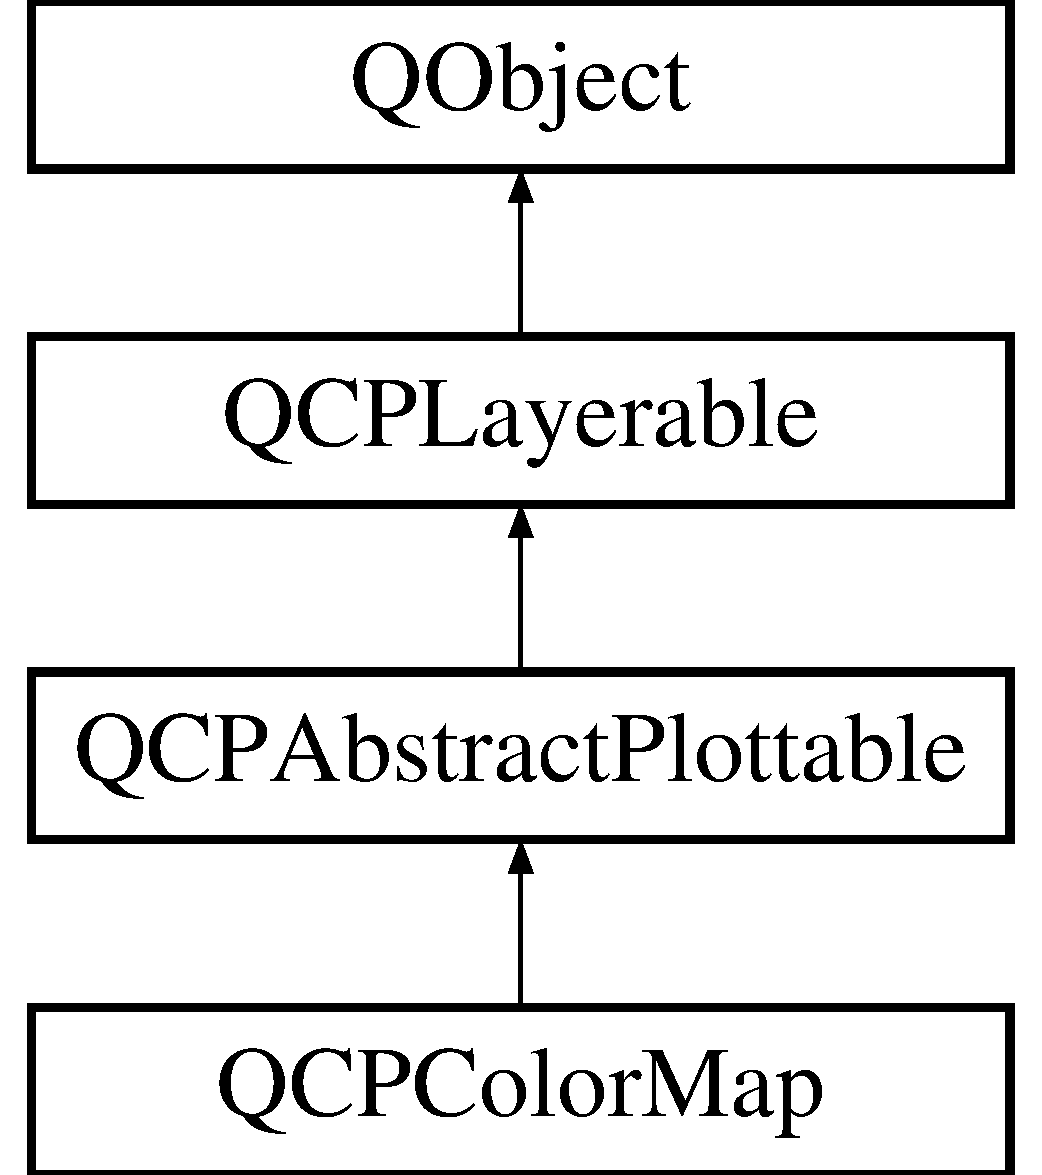
\includegraphics[height=4.000000cm]{class_q_c_p_color_map}
\end{center}
\end{figure}
\subsection*{Signals}
\begin{DoxyCompactItemize}
\item 
void \hyperlink{class_q_c_p_color_map_a482980f2335d09cfb36dd95ba9663197}{data\+Range\+Changed} (\hyperlink{class_q_c_p_range}{Q\+C\+P\+Range} new\+Range)
\item 
void \hyperlink{class_q_c_p_color_map_a978d5d5c9f68cffef8c902b855c04490}{data\+Scale\+Type\+Changed} (\hyperlink{class_q_c_p_axis_a36d8e8658dbaa179bf2aeb973db2d6f0}{Q\+C\+P\+Axis\+::\+Scale\+Type} scale\+Type)
\item 
void \hyperlink{class_q_c_p_color_map_abf4797f86e422ac6e0f732c4ff1a4d49}{gradient\+Changed} (\hyperlink{class_q_c_p_color_gradient}{Q\+C\+P\+Color\+Gradient} new\+Gradient)
\end{DoxyCompactItemize}
\subsection*{Public Member Functions}
\begin{DoxyCompactItemize}
\item 
\hyperlink{class_q_c_p_color_map_aa37e976d2ee1e2be6c4cd88a64b36215}{Q\+C\+P\+Color\+Map} (\hyperlink{class_q_c_p_axis}{Q\+C\+P\+Axis} $\ast$key\+Axis, \hyperlink{class_q_c_p_axis}{Q\+C\+P\+Axis} $\ast$value\+Axis)
\item 
\hyperlink{class_q_c_p_color_map_data}{Q\+C\+P\+Color\+Map\+Data} $\ast$ \hyperlink{class_q_c_p_color_map_a047d7eb3ae657f93f2f39b5e68b79451}{data} () const
\item 
\hypertarget{class_q_c_p_color_map_ae478f0a5a016420d66c70cc33d6cda1d}{}\label{class_q_c_p_color_map_ae478f0a5a016420d66c70cc33d6cda1d} 
\hyperlink{class_q_c_p_range}{Q\+C\+P\+Range} {\bfseries data\+Range} () const
\item 
\hypertarget{class_q_c_p_color_map_ab796f2dccc90fb7a354b6732c33ec9be}{}\label{class_q_c_p_color_map_ab796f2dccc90fb7a354b6732c33ec9be} 
\hyperlink{class_q_c_p_axis_a36d8e8658dbaa179bf2aeb973db2d6f0}{Q\+C\+P\+Axis\+::\+Scale\+Type} {\bfseries data\+Scale\+Type} () const
\item 
\hypertarget{class_q_c_p_color_map_a15d1877883fa463d44bfcbfd6840d4ca}{}\label{class_q_c_p_color_map_a15d1877883fa463d44bfcbfd6840d4ca} 
bool {\bfseries interpolate} () const
\item 
\hypertarget{class_q_c_p_color_map_a53b5d26b28d6027af0fc863f057965db}{}\label{class_q_c_p_color_map_a53b5d26b28d6027af0fc863f057965db} 
bool {\bfseries tight\+Boundary} () const
\item 
\hypertarget{class_q_c_p_color_map_acc4bb87c903607b96c08d2bc34bc24cd}{}\label{class_q_c_p_color_map_acc4bb87c903607b96c08d2bc34bc24cd} 
\hyperlink{class_q_c_p_color_gradient}{Q\+C\+P\+Color\+Gradient} {\bfseries gradient} () const
\item 
\hypertarget{class_q_c_p_color_map_a9d37d08c467ac645b86fc71a3b151208}{}\label{class_q_c_p_color_map_a9d37d08c467ac645b86fc71a3b151208} 
\hyperlink{class_q_c_p_color_scale}{Q\+C\+P\+Color\+Scale} $\ast$ {\bfseries color\+Scale} () const
\item 
void \hyperlink{class_q_c_p_color_map_a5a23e133a20c4ccad35fd32e6c0f9809}{set\+Data} (\hyperlink{class_q_c_p_color_map_data}{Q\+C\+P\+Color\+Map\+Data} $\ast$\hyperlink{class_q_c_p_color_map_a047d7eb3ae657f93f2f39b5e68b79451}{data}, bool copy=false)
\item 
Q\+\_\+\+S\+L\+OT void \hyperlink{class_q_c_p_color_map_a980b42837821159786a85b4b7dcb8774}{set\+Data\+Range} (const \hyperlink{class_q_c_p_range}{Q\+C\+P\+Range} \&data\+Range)
\item 
Q\+\_\+\+S\+L\+OT void \hyperlink{class_q_c_p_color_map_a9d20aa08e3c1f20f22908c45b9c06511}{set\+Data\+Scale\+Type} (\hyperlink{class_q_c_p_axis_a36d8e8658dbaa179bf2aeb973db2d6f0}{Q\+C\+P\+Axis\+::\+Scale\+Type} scale\+Type)
\item 
Q\+\_\+\+S\+L\+OT void \hyperlink{class_q_c_p_color_map_a7313c78360471cead3576341a2c50377}{set\+Gradient} (const \hyperlink{class_q_c_p_color_gradient}{Q\+C\+P\+Color\+Gradient} \&gradient)
\item 
void \hyperlink{class_q_c_p_color_map_a484eaa8a5065cfc386b15375bf98b964}{set\+Interpolate} (bool enabled)
\item 
void \hyperlink{class_q_c_p_color_map_ad03221cc285e5f562a0b13d684b5576d}{set\+Tight\+Boundary} (bool enabled)
\item 
void \hyperlink{class_q_c_p_color_map_aa828921db364fe3c6af4619580ab85fd}{set\+Color\+Scale} (\hyperlink{class_q_c_p_color_scale}{Q\+C\+P\+Color\+Scale} $\ast$color\+Scale)
\item 
void \hyperlink{class_q_c_p_color_map_a856608fa3dd1cc290bcd5f29a5575774}{rescale\+Data\+Range} (bool recalculate\+Data\+Bounds=false)
\item 
Q\+\_\+\+S\+L\+OT void \hyperlink{class_q_c_p_color_map_a5d8158b62d55fcfeaabcb68ce0083e87}{update\+Legend\+Icon} (Qt\+::\+Transformation\+Mode transform\+Mode=Qt\+::\+Smooth\+Transformation, const Q\+Size \&thumb\+Size=Q\+Size(32, 18))
\item 
virtual void \hyperlink{class_q_c_p_color_map_a0545dce5383766885912331705a8e099}{clear\+Data} ()
\item 
virtual double \hyperlink{class_q_c_p_color_map_aba91ea58b489031157ecb777fe79e309}{select\+Test} (const Q\+PointF \&pos, bool only\+Selectable, Q\+Variant $\ast$details=0) const
\end{DoxyCompactItemize}
\subsection*{Protected Member Functions}
\begin{DoxyCompactItemize}
\item 
\hypertarget{class_q_c_p_color_map_a5efcea591bb5486d968af520a4d43c3a}{}\label{class_q_c_p_color_map_a5efcea591bb5486d968af520a4d43c3a} 
virtual void {\bfseries update\+Map\+Image} ()
\item 
\hypertarget{class_q_c_p_color_map_a3b0f45a3177be9522d5e9b8cd8ae122d}{}\label{class_q_c_p_color_map_a3b0f45a3177be9522d5e9b8cd8ae122d} 
virtual void {\bfseries draw} (\hyperlink{class_q_c_p_painter}{Q\+C\+P\+Painter} $\ast$painter)
\item 
\hypertarget{class_q_c_p_color_map_a63584cbf7aa7463e81b58f6e4254423b}{}\label{class_q_c_p_color_map_a63584cbf7aa7463e81b58f6e4254423b} 
virtual void {\bfseries draw\+Legend\+Icon} (\hyperlink{class_q_c_p_painter}{Q\+C\+P\+Painter} $\ast$painter, const Q\+RectF \&rect) const
\item 
\hypertarget{class_q_c_p_color_map_af294ea4d207e6e3411fb05c69e2c7fa9}{}\label{class_q_c_p_color_map_af294ea4d207e6e3411fb05c69e2c7fa9} 
virtual \hyperlink{class_q_c_p_range}{Q\+C\+P\+Range} {\bfseries get\+Key\+Range} (bool \&found\+Range, \hyperlink{class_q_c_p_abstract_plottable_a661743478a1d3c09d28ec2711d7653d8}{Sign\+Domain} in\+Sign\+Domain=\hyperlink{class_q_c_p_abstract_plottable_a661743478a1d3c09d28ec2711d7653d8a082b98cfb91a7363a3b5cd17b0c1cd60}{sd\+Both}) const
\item 
\hypertarget{class_q_c_p_color_map_a06cebc3006df6a156be2c9395be6fa0b}{}\label{class_q_c_p_color_map_a06cebc3006df6a156be2c9395be6fa0b} 
virtual \hyperlink{class_q_c_p_range}{Q\+C\+P\+Range} {\bfseries get\+Value\+Range} (bool \&found\+Range, \hyperlink{class_q_c_p_abstract_plottable_a661743478a1d3c09d28ec2711d7653d8}{Sign\+Domain} in\+Sign\+Domain=\hyperlink{class_q_c_p_abstract_plottable_a661743478a1d3c09d28ec2711d7653d8a082b98cfb91a7363a3b5cd17b0c1cd60}{sd\+Both}) const
\end{DoxyCompactItemize}
\subsection*{Protected Attributes}
\begin{DoxyCompactItemize}
\item 
\hypertarget{class_q_c_p_color_map_ab87609621d16cd3e9d52ad070b327b08}{}\label{class_q_c_p_color_map_ab87609621d16cd3e9d52ad070b327b08} 
\hyperlink{class_q_c_p_range}{Q\+C\+P\+Range} {\bfseries m\+Data\+Range}
\item 
\hypertarget{class_q_c_p_color_map_ab28a4b2def408f83b9818799d5f18446}{}\label{class_q_c_p_color_map_ab28a4b2def408f83b9818799d5f18446} 
\hyperlink{class_q_c_p_axis_a36d8e8658dbaa179bf2aeb973db2d6f0}{Q\+C\+P\+Axis\+::\+Scale\+Type} {\bfseries m\+Data\+Scale\+Type}
\item 
\hypertarget{class_q_c_p_color_map_a8709272aa8f0be3ca111bf3866806f8b}{}\label{class_q_c_p_color_map_a8709272aa8f0be3ca111bf3866806f8b} 
\hyperlink{class_q_c_p_color_map_data}{Q\+C\+P\+Color\+Map\+Data} $\ast$ {\bfseries m\+Map\+Data}
\item 
\hypertarget{class_q_c_p_color_map_aab77fe9a8df6f0486ab3507cc5f278fa}{}\label{class_q_c_p_color_map_aab77fe9a8df6f0486ab3507cc5f278fa} 
\hyperlink{class_q_c_p_color_gradient}{Q\+C\+P\+Color\+Gradient} {\bfseries m\+Gradient}
\item 
\hypertarget{class_q_c_p_color_map_af77e5eba9a844592648edeb6fbe834f1}{}\label{class_q_c_p_color_map_af77e5eba9a844592648edeb6fbe834f1} 
bool {\bfseries m\+Interpolate}
\item 
\hypertarget{class_q_c_p_color_map_ac2e9425fe4381b496726e1c09f978302}{}\label{class_q_c_p_color_map_ac2e9425fe4381b496726e1c09f978302} 
bool {\bfseries m\+Tight\+Boundary}
\item 
\hypertarget{class_q_c_p_color_map_a95b4100bacc3387652c988b071ec9db7}{}\label{class_q_c_p_color_map_a95b4100bacc3387652c988b071ec9db7} 
Q\+Pointer$<$ \hyperlink{class_q_c_p_color_scale}{Q\+C\+P\+Color\+Scale} $>$ {\bfseries m\+Color\+Scale}
\item 
\hypertarget{class_q_c_p_color_map_a66110813b42eca78b64095b2a1f285a0}{}\label{class_q_c_p_color_map_a66110813b42eca78b64095b2a1f285a0} 
Q\+Image {\bfseries m\+Map\+Image}
\item 
\hypertarget{class_q_c_p_color_map_acad3d52f3572436d5f2e4057911ea8d3}{}\label{class_q_c_p_color_map_acad3d52f3572436d5f2e4057911ea8d3} 
Q\+Image {\bfseries m\+Undersampled\+Map\+Image}
\item 
\hypertarget{class_q_c_p_color_map_ada522988db02cb531767d38c5029ef60}{}\label{class_q_c_p_color_map_ada522988db02cb531767d38c5029ef60} 
Q\+Pixmap {\bfseries m\+Legend\+Icon}
\item 
\hypertarget{class_q_c_p_color_map_ac9aea6a5c193d7fa866bc7b26e79ef2c}{}\label{class_q_c_p_color_map_ac9aea6a5c193d7fa866bc7b26e79ef2c} 
bool {\bfseries m\+Map\+Image\+Invalidated}
\end{DoxyCompactItemize}
\subsection*{Friends}
\begin{DoxyCompactItemize}
\item 
\hypertarget{class_q_c_p_color_map_a1cdf9df76adcfae45261690aa0ca2198}{}\label{class_q_c_p_color_map_a1cdf9df76adcfae45261690aa0ca2198} 
class {\bfseries Q\+Custom\+Plot}
\item 
\hypertarget{class_q_c_p_color_map_a8429035e7adfbd7f05805a6530ad5e3b}{}\label{class_q_c_p_color_map_a8429035e7adfbd7f05805a6530ad5e3b} 
class {\bfseries Q\+C\+P\+Legend}
\end{DoxyCompactItemize}
\subsection*{Additional Inherited Members}


\subsection{Detailed Description}
A plottable representing a two-\/dimensional color map in a plot. 



The data is stored in the class \hyperlink{class_q_c_p_color_map_data}{Q\+C\+P\+Color\+Map\+Data}, which can be accessed via the \hyperlink{class_q_c_p_color_map_a047d7eb3ae657f93f2f39b5e68b79451}{data()} method.

A color map has three dimensions to represent a data point\+: The {\itshape key} dimension, the {\itshape value} dimension and the {\itshape data} dimension. As with other plottables such as graphs, {\itshape key} and {\itshape value} correspond to two orthogonal axes on the \hyperlink{class_q_custom_plot}{Q\+Custom\+Plot} surface that you specify in the \hyperlink{class_q_c_p_color_map}{Q\+C\+P\+Color\+Map} constructor. The {\itshape data} dimension however is encoded as the color of the point at ({\itshape key}, {\itshape value}).

Set the number of points (or {\itshape cells}) in the key/value dimension via \hyperlink{class_q_c_p_color_map_data_a0d9ff35c299d0478b682bfbcdd9c097e}{Q\+C\+P\+Color\+Map\+Data\+::set\+Size}. The plot coordinate range over which these points will be displayed is specified via \hyperlink{class_q_c_p_color_map_data_aad9c1c7c703c1339489fc730517c83d4}{Q\+C\+P\+Color\+Map\+Data\+::set\+Range}. The first cell will be centered on the lower range boundary and the last cell will be centered on the upper range boundary. The data can be set by either accessing the cells directly with \hyperlink{class_q_c_p_color_map_data_a8e75eaf8746596319032a93f3d2d0683}{Q\+C\+P\+Color\+Map\+Data\+::set\+Cell} or by addressing the cells via their plot coordinates with \hyperlink{class_q_c_p_color_map_data_afd2083ccfd6987ec94aa7ef8e91ca39a}{Q\+C\+P\+Color\+Map\+Data\+::set\+Data}. If possible, you should prefer set\+Cell, since it doesn\textquotesingle{}t need to do any coordinate transformation and thus performs a bit better.

The cell with index (0, 0) is at the bottom left, if the color map uses normal (i.\+e. not reversed) key and value axes.

To show the user which colors correspond to which {\itshape data} values, a \hyperlink{class_q_c_p_color_scale}{Q\+C\+P\+Color\+Scale} is typically placed to the right of the axis rect. See the documentation there for details on how to add and use a color scale.\hypertarget{class_q_c_p_statistical_box_appearance}{}\subsection{Changing the appearance}\label{class_q_c_p_statistical_box_appearance}
The central part of the appearance is the color gradient, which can be specified via \hyperlink{class_q_c_p_color_map_a7313c78360471cead3576341a2c50377}{set\+Gradient}. See the documentation of \hyperlink{class_q_c_p_color_gradient}{Q\+C\+P\+Color\+Gradient} for details on configuring a color gradient.

The {\itshape data} range that is mapped to the colors of the gradient can be specified with \hyperlink{class_q_c_p_color_map_a980b42837821159786a85b4b7dcb8774}{set\+Data\+Range}. To make the data range encompass the whole data set minimum to maximum, call \hyperlink{class_q_c_p_color_map_a856608fa3dd1cc290bcd5f29a5575774}{rescale\+Data\+Range}.\hypertarget{class_q_c_p_statistical_box_usage}{}\subsection{Usage}\label{class_q_c_p_statistical_box_usage}
Like all data representing objects in \hyperlink{class_q_custom_plot}{Q\+Custom\+Plot}, the \hyperlink{class_q_c_p_color_map}{Q\+C\+P\+Color\+Map} is a plottable (\hyperlink{class_q_c_p_abstract_plottable}{Q\+C\+P\+Abstract\+Plottable}). So the plottable-\/interface of \hyperlink{class_q_custom_plot}{Q\+Custom\+Plot} applies (\hyperlink{class_q_custom_plot_a32de81ff53e263e785b83b52ecd99d6f}{Q\+Custom\+Plot\+::plottable}, \hyperlink{class_q_custom_plot_ab7ad9174f701f9c6f64e378df77927a6}{Q\+Custom\+Plot\+::add\+Plottable}, \hyperlink{class_q_custom_plot_af3dafd56884208474f311d6226513ab2}{Q\+Custom\+Plot\+::remove\+Plottable}, etc.)

Usually, you first create an instance and add it to the custom\+Plot\+: 
\begin{DoxyCodeInclude}
\end{DoxyCodeInclude}
and then modify the properties of the newly created color map, e.\+g.\+: 
\begin{DoxyCodeInclude}
\end{DoxyCodeInclude}
 \begin{DoxyNote}{Note}
The \hyperlink{class_q_c_p_color_map}{Q\+C\+P\+Color\+Map} always displays the data at equal key/value intervals, even if the key or value axis is set to a logarithmic scaling. If you want to use \hyperlink{class_q_c_p_color_map}{Q\+C\+P\+Color\+Map} with logarithmic axes, you shouldn\textquotesingle{}t use the \hyperlink{class_q_c_p_color_map_data_afd2083ccfd6987ec94aa7ef8e91ca39a}{Q\+C\+P\+Color\+Map\+Data\+::set\+Data} method as it uses a linear transformation to determine the cell index. Rather directly access the cell index with \hyperlink{class_q_c_p_color_map_data_a8e75eaf8746596319032a93f3d2d0683}{Q\+C\+P\+Color\+Map\+Data\+::set\+Cell}. 
\end{DoxyNote}


\subsection{Constructor \& Destructor Documentation}
\hypertarget{class_q_c_p_color_map_aa37e976d2ee1e2be6c4cd88a64b36215}{}\label{class_q_c_p_color_map_aa37e976d2ee1e2be6c4cd88a64b36215} 
\index{Q\+C\+P\+Color\+Map@{Q\+C\+P\+Color\+Map}!Q\+C\+P\+Color\+Map@{Q\+C\+P\+Color\+Map}}
\index{Q\+C\+P\+Color\+Map@{Q\+C\+P\+Color\+Map}!Q\+C\+P\+Color\+Map@{Q\+C\+P\+Color\+Map}}
\subsubsection{\texorpdfstring{Q\+C\+P\+Color\+Map()}{QCPColorMap()}}
{\footnotesize\ttfamily Q\+C\+P\+Color\+Map\+::\+Q\+C\+P\+Color\+Map (\begin{DoxyParamCaption}\item[{\hyperlink{class_q_c_p_axis}{Q\+C\+P\+Axis} $\ast$}]{key\+Axis,  }\item[{\hyperlink{class_q_c_p_axis}{Q\+C\+P\+Axis} $\ast$}]{value\+Axis }\end{DoxyParamCaption})\hspace{0.3cm}{\ttfamily [explicit]}}

Constructs a color map with the specified {\itshape key\+Axis} and {\itshape value\+Axis}.

The constructed \hyperlink{class_q_c_p_color_map}{Q\+C\+P\+Color\+Map} can be added to the plot with \hyperlink{class_q_custom_plot_ab7ad9174f701f9c6f64e378df77927a6}{Q\+Custom\+Plot\+::add\+Plottable}, \hyperlink{class_q_custom_plot}{Q\+Custom\+Plot} then takes ownership of the color map. 

\subsection{Member Function Documentation}
\hypertarget{class_q_c_p_color_map_a0545dce5383766885912331705a8e099}{}\label{class_q_c_p_color_map_a0545dce5383766885912331705a8e099} 
\index{Q\+C\+P\+Color\+Map@{Q\+C\+P\+Color\+Map}!clear\+Data@{clear\+Data}}
\index{clear\+Data@{clear\+Data}!Q\+C\+P\+Color\+Map@{Q\+C\+P\+Color\+Map}}
\subsubsection{\texorpdfstring{clear\+Data()}{clearData()}}
{\footnotesize\ttfamily void Q\+C\+P\+Color\+Map\+::clear\+Data (\begin{DoxyParamCaption}{ }\end{DoxyParamCaption})\hspace{0.3cm}{\ttfamily [virtual]}}

Clears the colormap data by calling \hyperlink{class_q_c_p_color_map_data_a9910ba830e96955bd5c8e5bef1e77ef3}{Q\+C\+P\+Color\+Map\+Data\+::clear()} on the internal data. This also resizes the map to 0x0 cells. 

Implements \hyperlink{class_q_c_p_abstract_plottable_a86e5b8fd4b6ff4f4084e7ea4c573fc53}{Q\+C\+P\+Abstract\+Plottable}.

\hypertarget{class_q_c_p_color_map_a047d7eb3ae657f93f2f39b5e68b79451}{}\label{class_q_c_p_color_map_a047d7eb3ae657f93f2f39b5e68b79451} 
\index{Q\+C\+P\+Color\+Map@{Q\+C\+P\+Color\+Map}!data@{data}}
\index{data@{data}!Q\+C\+P\+Color\+Map@{Q\+C\+P\+Color\+Map}}
\subsubsection{\texorpdfstring{data()}{data()}}
{\footnotesize\ttfamily \hyperlink{class_q_c_p_color_map_data}{Q\+C\+P\+Color\+Map\+Data} $\ast$ Q\+C\+P\+Color\+Map\+::data (\begin{DoxyParamCaption}{ }\end{DoxyParamCaption}) const\hspace{0.3cm}{\ttfamily [inline]}}

Returns a pointer to the internal data storage of type \hyperlink{class_q_c_p_color_map_data}{Q\+C\+P\+Color\+Map\+Data}. Access this to modify data points (cells) and the color map key/value range.

\begin{DoxySeeAlso}{See also}
\hyperlink{class_q_c_p_color_map_a5a23e133a20c4ccad35fd32e6c0f9809}{set\+Data} 
\end{DoxySeeAlso}
\hypertarget{class_q_c_p_color_map_a482980f2335d09cfb36dd95ba9663197}{}\label{class_q_c_p_color_map_a482980f2335d09cfb36dd95ba9663197} 
\index{Q\+C\+P\+Color\+Map@{Q\+C\+P\+Color\+Map}!data\+Range\+Changed@{data\+Range\+Changed}}
\index{data\+Range\+Changed@{data\+Range\+Changed}!Q\+C\+P\+Color\+Map@{Q\+C\+P\+Color\+Map}}
\subsubsection{\texorpdfstring{data\+Range\+Changed}{dataRangeChanged}}
{\footnotesize\ttfamily void Q\+C\+P\+Color\+Map\+::data\+Range\+Changed (\begin{DoxyParamCaption}\item[{\hyperlink{class_q_c_p_range}{Q\+C\+P\+Range}}]{new\+Range }\end{DoxyParamCaption})\hspace{0.3cm}{\ttfamily [signal]}}

This signal is emitted when the data range changes.

\begin{DoxySeeAlso}{See also}
\hyperlink{class_q_c_p_color_map_a980b42837821159786a85b4b7dcb8774}{set\+Data\+Range} 
\end{DoxySeeAlso}
\hypertarget{class_q_c_p_color_map_a978d5d5c9f68cffef8c902b855c04490}{}\label{class_q_c_p_color_map_a978d5d5c9f68cffef8c902b855c04490} 
\index{Q\+C\+P\+Color\+Map@{Q\+C\+P\+Color\+Map}!data\+Scale\+Type\+Changed@{data\+Scale\+Type\+Changed}}
\index{data\+Scale\+Type\+Changed@{data\+Scale\+Type\+Changed}!Q\+C\+P\+Color\+Map@{Q\+C\+P\+Color\+Map}}
\subsubsection{\texorpdfstring{data\+Scale\+Type\+Changed}{dataScaleTypeChanged}}
{\footnotesize\ttfamily void Q\+C\+P\+Color\+Map\+::data\+Scale\+Type\+Changed (\begin{DoxyParamCaption}\item[{\hyperlink{class_q_c_p_axis_a36d8e8658dbaa179bf2aeb973db2d6f0}{Q\+C\+P\+Axis\+::\+Scale\+Type}}]{scale\+Type }\end{DoxyParamCaption})\hspace{0.3cm}{\ttfamily [signal]}}

This signal is emitted when the data scale type changes.

\begin{DoxySeeAlso}{See also}
\hyperlink{class_q_c_p_color_map_a9d20aa08e3c1f20f22908c45b9c06511}{set\+Data\+Scale\+Type} 
\end{DoxySeeAlso}
\hypertarget{class_q_c_p_color_map_abf4797f86e422ac6e0f732c4ff1a4d49}{}\label{class_q_c_p_color_map_abf4797f86e422ac6e0f732c4ff1a4d49} 
\index{Q\+C\+P\+Color\+Map@{Q\+C\+P\+Color\+Map}!gradient\+Changed@{gradient\+Changed}}
\index{gradient\+Changed@{gradient\+Changed}!Q\+C\+P\+Color\+Map@{Q\+C\+P\+Color\+Map}}
\subsubsection{\texorpdfstring{gradient\+Changed}{gradientChanged}}
{\footnotesize\ttfamily void Q\+C\+P\+Color\+Map\+::gradient\+Changed (\begin{DoxyParamCaption}\item[{\hyperlink{class_q_c_p_color_gradient}{Q\+C\+P\+Color\+Gradient}}]{new\+Gradient }\end{DoxyParamCaption})\hspace{0.3cm}{\ttfamily [signal]}}

This signal is emitted when the gradient changes.

\begin{DoxySeeAlso}{See also}
\hyperlink{class_q_c_p_color_map_a7313c78360471cead3576341a2c50377}{set\+Gradient} 
\end{DoxySeeAlso}
\hypertarget{class_q_c_p_color_map_a856608fa3dd1cc290bcd5f29a5575774}{}\label{class_q_c_p_color_map_a856608fa3dd1cc290bcd5f29a5575774} 
\index{Q\+C\+P\+Color\+Map@{Q\+C\+P\+Color\+Map}!rescale\+Data\+Range@{rescale\+Data\+Range}}
\index{rescale\+Data\+Range@{rescale\+Data\+Range}!Q\+C\+P\+Color\+Map@{Q\+C\+P\+Color\+Map}}
\subsubsection{\texorpdfstring{rescale\+Data\+Range()}{rescaleDataRange()}}
{\footnotesize\ttfamily void Q\+C\+P\+Color\+Map\+::rescale\+Data\+Range (\begin{DoxyParamCaption}\item[{bool}]{recalculate\+Data\+Bounds = {\ttfamily false} }\end{DoxyParamCaption})}

Sets the data range (\hyperlink{class_q_c_p_color_map_a980b42837821159786a85b4b7dcb8774}{set\+Data\+Range}) to span the minimum and maximum values that occur in the current data set. This corresponds to the \hyperlink{class_q_c_p_abstract_plottable_ae96b83c961e257da116c6acf9c7da308}{rescale\+Key\+Axis} or \hyperlink{class_q_c_p_abstract_plottable_aa1e408bb2d13999150c3f7f8a8579ca9}{rescale\+Value\+Axis} methods, only for the third data dimension of the color map.

The minimum and maximum values of the data set are buffered in the internal \hyperlink{class_q_c_p_color_map_data}{Q\+C\+P\+Color\+Map\+Data} instance (\hyperlink{class_q_c_p_color_map_a047d7eb3ae657f93f2f39b5e68b79451}{data}). As data is updated via its \hyperlink{class_q_c_p_color_map_data_a8e75eaf8746596319032a93f3d2d0683}{Q\+C\+P\+Color\+Map\+Data\+::set\+Cell} or \hyperlink{class_q_c_p_color_map_data_afd2083ccfd6987ec94aa7ef8e91ca39a}{Q\+C\+P\+Color\+Map\+Data\+::set\+Data}, the buffered minimum and maximum values are updated, too. For performance reasons, however, they are only updated in an expanding fashion. So the buffered maximum can only increase and the buffered minimum can only decrease. In consequence, changes to the data that actually lower the maximum of the data set (by overwriting the cell holding the current maximum with a smaller value), aren\textquotesingle{}t recognized and the buffered maximum overestimates the true maximum of the data set. The same happens for the buffered minimum. To recalculate the true minimum and maximum by explicitly looking at each cell, the method \hyperlink{class_q_c_p_color_map_data_ab235ade8a4d64bd3adb26a99b3dd57ee}{Q\+C\+P\+Color\+Map\+Data\+::recalculate\+Data\+Bounds} can be used. For convenience, setting the parameter {\itshape recalculate\+Data\+Bounds} calls this method before setting the data range to the buffered minimum and maximum.

\begin{DoxySeeAlso}{See also}
\hyperlink{class_q_c_p_color_map_a980b42837821159786a85b4b7dcb8774}{set\+Data\+Range} 
\end{DoxySeeAlso}
\hypertarget{class_q_c_p_color_map_aba91ea58b489031157ecb777fe79e309}{}\label{class_q_c_p_color_map_aba91ea58b489031157ecb777fe79e309} 
\index{Q\+C\+P\+Color\+Map@{Q\+C\+P\+Color\+Map}!select\+Test@{select\+Test}}
\index{select\+Test@{select\+Test}!Q\+C\+P\+Color\+Map@{Q\+C\+P\+Color\+Map}}
\subsubsection{\texorpdfstring{select\+Test()}{selectTest()}}
{\footnotesize\ttfamily double Q\+C\+P\+Color\+Map\+::select\+Test (\begin{DoxyParamCaption}\item[{const Q\+PointF \&}]{pos,  }\item[{bool}]{only\+Selectable,  }\item[{Q\+Variant $\ast$}]{details = {\ttfamily 0} }\end{DoxyParamCaption}) const\hspace{0.3cm}{\ttfamily [virtual]}}

This function is used to decide whether a click hits a layerable object or not.

{\itshape pos} is a point in pixel coordinates on the \hyperlink{class_q_custom_plot}{Q\+Custom\+Plot} surface. This function returns the shortest pixel distance of this point to the object. If the object is either invisible or the distance couldn\textquotesingle{}t be determined, -\/1.\+0 is returned. Further, if {\itshape only\+Selectable} is true and the object is not selectable, -\/1.\+0 is returned, too.

If the object is represented not by single lines but by an area like a \hyperlink{class_q_c_p_item_text}{Q\+C\+P\+Item\+Text} or the bars of a \hyperlink{class_q_c_p_bars}{Q\+C\+P\+Bars} plottable, a click inside the area should also be considered a hit. In these cases this function thus returns a constant value greater zero but still below the parent plot\textquotesingle{}s selection tolerance. (typically the selection\+Tolerance multiplied by 0.\+99).

Providing a constant value for area objects allows selecting line objects even when they are obscured by such area objects, by clicking close to the lines (i.\+e. closer than 0.\+99$\ast$selection\+Tolerance).

The actual setting of the selection state is not done by this function. This is handled by the parent \hyperlink{class_q_custom_plot}{Q\+Custom\+Plot} when the mouse\+Release\+Event occurs, and the finally selected object is notified via the select\+Event/deselect\+Event methods.

{\itshape details} is an optional output parameter. Every layerable subclass may place any information in {\itshape details}. This information will be passed to select\+Event when the parent \hyperlink{class_q_custom_plot}{Q\+Custom\+Plot} decides on the basis of this select\+Test call, that the object was successfully selected. The subsequent call to select\+Event will carry the {\itshape details}. This is useful for multi-\/part objects (like \hyperlink{class_q_c_p_axis}{Q\+C\+P\+Axis}). This way, a possibly complex calculation to decide which part was clicked is only done once in \hyperlink{class_q_c_p_color_map_aba91ea58b489031157ecb777fe79e309}{select\+Test}. The result (i.\+e. the actually clicked part) can then be placed in {\itshape details}. So in the subsequent select\+Event, the decision which part was selected doesn\textquotesingle{}t have to be done a second time for a single selection operation.

You may pass 0 as {\itshape details} to indicate that you are not interested in those selection details.

\begin{DoxySeeAlso}{See also}
select\+Event, deselect\+Event, \hyperlink{class_q_custom_plot_a5ee1e2f6ae27419deca53e75907c27e5}{Q\+Custom\+Plot\+::set\+Interactions} 
\end{DoxySeeAlso}


Implements \hyperlink{class_q_c_p_abstract_plottable_a38efe9641d972992a3d44204bc80ec1d}{Q\+C\+P\+Abstract\+Plottable}.

\hypertarget{class_q_c_p_color_map_aa828921db364fe3c6af4619580ab85fd}{}\label{class_q_c_p_color_map_aa828921db364fe3c6af4619580ab85fd} 
\index{Q\+C\+P\+Color\+Map@{Q\+C\+P\+Color\+Map}!set\+Color\+Scale@{set\+Color\+Scale}}
\index{set\+Color\+Scale@{set\+Color\+Scale}!Q\+C\+P\+Color\+Map@{Q\+C\+P\+Color\+Map}}
\subsubsection{\texorpdfstring{set\+Color\+Scale()}{setColorScale()}}
{\footnotesize\ttfamily void Q\+C\+P\+Color\+Map\+::set\+Color\+Scale (\begin{DoxyParamCaption}\item[{\hyperlink{class_q_c_p_color_scale}{Q\+C\+P\+Color\+Scale} $\ast$}]{color\+Scale }\end{DoxyParamCaption})}

Associates the color scale {\itshape color\+Scale} with this color map.

This means that both the color scale and the color map synchronize their gradient, data range and data scale type (\hyperlink{class_q_c_p_color_map_a7313c78360471cead3576341a2c50377}{set\+Gradient}, \hyperlink{class_q_c_p_color_map_a980b42837821159786a85b4b7dcb8774}{set\+Data\+Range}, \hyperlink{class_q_c_p_color_map_a9d20aa08e3c1f20f22908c45b9c06511}{set\+Data\+Scale\+Type}). Multiple color maps can be associated with one single color scale. This causes the color maps to also synchronize those properties, via the mutual color scale.

This function causes the color map to adopt the current color gradient, data range and data scale type of {\itshape color\+Scale}. After this call, you may change these properties at either the color map or the color scale, and the setting will be applied to both.

Pass 0 as {\itshape color\+Scale} to disconnect the color scale from this color map again. \hypertarget{class_q_c_p_color_map_a5a23e133a20c4ccad35fd32e6c0f9809}{}\label{class_q_c_p_color_map_a5a23e133a20c4ccad35fd32e6c0f9809} 
\index{Q\+C\+P\+Color\+Map@{Q\+C\+P\+Color\+Map}!set\+Data@{set\+Data}}
\index{set\+Data@{set\+Data}!Q\+C\+P\+Color\+Map@{Q\+C\+P\+Color\+Map}}
\subsubsection{\texorpdfstring{set\+Data()}{setData()}}
{\footnotesize\ttfamily void Q\+C\+P\+Color\+Map\+::set\+Data (\begin{DoxyParamCaption}\item[{\hyperlink{class_q_c_p_color_map_data}{Q\+C\+P\+Color\+Map\+Data} $\ast$}]{data,  }\item[{bool}]{copy = {\ttfamily false} }\end{DoxyParamCaption})}

Replaces the current \hyperlink{class_q_c_p_color_map_a047d7eb3ae657f93f2f39b5e68b79451}{data} with the provided {\itshape data}.

If {\itshape copy} is set to true, the {\itshape data} object will only be copied. if false, the color map takes ownership of the passed data and replaces the internal data pointer with it. This is significantly faster than copying for large datasets. \hypertarget{class_q_c_p_color_map_a980b42837821159786a85b4b7dcb8774}{}\label{class_q_c_p_color_map_a980b42837821159786a85b4b7dcb8774} 
\index{Q\+C\+P\+Color\+Map@{Q\+C\+P\+Color\+Map}!set\+Data\+Range@{set\+Data\+Range}}
\index{set\+Data\+Range@{set\+Data\+Range}!Q\+C\+P\+Color\+Map@{Q\+C\+P\+Color\+Map}}
\subsubsection{\texorpdfstring{set\+Data\+Range()}{setDataRange()}}
{\footnotesize\ttfamily void Q\+C\+P\+Color\+Map\+::set\+Data\+Range (\begin{DoxyParamCaption}\item[{const \hyperlink{class_q_c_p_range}{Q\+C\+P\+Range} \&}]{data\+Range }\end{DoxyParamCaption})}

Sets the data range of this color map to {\itshape data\+Range}. The data range defines which data values are mapped to the color gradient.

To make the data range span the full range of the data set, use \hyperlink{class_q_c_p_color_map_a856608fa3dd1cc290bcd5f29a5575774}{rescale\+Data\+Range}.

\begin{DoxySeeAlso}{See also}
\hyperlink{class_q_c_p_color_scale_abe88633003a26d1e756aa74984587fef}{Q\+C\+P\+Color\+Scale\+::set\+Data\+Range} 
\end{DoxySeeAlso}
\hypertarget{class_q_c_p_color_map_a9d20aa08e3c1f20f22908c45b9c06511}{}\label{class_q_c_p_color_map_a9d20aa08e3c1f20f22908c45b9c06511} 
\index{Q\+C\+P\+Color\+Map@{Q\+C\+P\+Color\+Map}!set\+Data\+Scale\+Type@{set\+Data\+Scale\+Type}}
\index{set\+Data\+Scale\+Type@{set\+Data\+Scale\+Type}!Q\+C\+P\+Color\+Map@{Q\+C\+P\+Color\+Map}}
\subsubsection{\texorpdfstring{set\+Data\+Scale\+Type()}{setDataScaleType()}}
{\footnotesize\ttfamily void Q\+C\+P\+Color\+Map\+::set\+Data\+Scale\+Type (\begin{DoxyParamCaption}\item[{\hyperlink{class_q_c_p_axis_a36d8e8658dbaa179bf2aeb973db2d6f0}{Q\+C\+P\+Axis\+::\+Scale\+Type}}]{scale\+Type }\end{DoxyParamCaption})}

Sets whether the data is correlated with the color gradient linearly or logarithmically.

\begin{DoxySeeAlso}{See also}
\hyperlink{class_q_c_p_color_scale_aeb6107d67dd7325145b2498abae67fc3}{Q\+C\+P\+Color\+Scale\+::set\+Data\+Scale\+Type} 
\end{DoxySeeAlso}
\hypertarget{class_q_c_p_color_map_a7313c78360471cead3576341a2c50377}{}\label{class_q_c_p_color_map_a7313c78360471cead3576341a2c50377} 
\index{Q\+C\+P\+Color\+Map@{Q\+C\+P\+Color\+Map}!set\+Gradient@{set\+Gradient}}
\index{set\+Gradient@{set\+Gradient}!Q\+C\+P\+Color\+Map@{Q\+C\+P\+Color\+Map}}
\subsubsection{\texorpdfstring{set\+Gradient()}{setGradient()}}
{\footnotesize\ttfamily void Q\+C\+P\+Color\+Map\+::set\+Gradient (\begin{DoxyParamCaption}\item[{const \hyperlink{class_q_c_p_color_gradient}{Q\+C\+P\+Color\+Gradient} \&}]{gradient }\end{DoxyParamCaption})}

Sets the color gradient that is used to represent the data. For more details on how to create an own gradient or use one of the preset gradients, see \hyperlink{class_q_c_p_color_gradient}{Q\+C\+P\+Color\+Gradient}.

The colors defined by the gradient will be used to represent data values in the currently set data range, see \hyperlink{class_q_c_p_color_map_a980b42837821159786a85b4b7dcb8774}{set\+Data\+Range}. Data points that are outside this data range will either be colored uniformly with the respective gradient boundary color, or the gradient will repeat, depending on \hyperlink{class_q_c_p_color_gradient_a39d6448155fc00a219f239220d14bb39}{Q\+C\+P\+Color\+Gradient\+::set\+Periodic}.

\begin{DoxySeeAlso}{See also}
\hyperlink{class_q_c_p_color_scale_a1f29583bb6f1e7f473b62fb712be3940}{Q\+C\+P\+Color\+Scale\+::set\+Gradient} 
\end{DoxySeeAlso}
\hypertarget{class_q_c_p_color_map_a484eaa8a5065cfc386b15375bf98b964}{}\label{class_q_c_p_color_map_a484eaa8a5065cfc386b15375bf98b964} 
\index{Q\+C\+P\+Color\+Map@{Q\+C\+P\+Color\+Map}!set\+Interpolate@{set\+Interpolate}}
\index{set\+Interpolate@{set\+Interpolate}!Q\+C\+P\+Color\+Map@{Q\+C\+P\+Color\+Map}}
\subsubsection{\texorpdfstring{set\+Interpolate()}{setInterpolate()}}
{\footnotesize\ttfamily void Q\+C\+P\+Color\+Map\+::set\+Interpolate (\begin{DoxyParamCaption}\item[{bool}]{enabled }\end{DoxyParamCaption})}

Sets whether the color map image shall use bicubic interpolation when displaying the color map shrinked or expanded, and not at a 1\+:1 pixel-\/to-\/data scale.

\hypertarget{class_q_c_p_color_map_ad03221cc285e5f562a0b13d684b5576d}{}\label{class_q_c_p_color_map_ad03221cc285e5f562a0b13d684b5576d} 
\index{Q\+C\+P\+Color\+Map@{Q\+C\+P\+Color\+Map}!set\+Tight\+Boundary@{set\+Tight\+Boundary}}
\index{set\+Tight\+Boundary@{set\+Tight\+Boundary}!Q\+C\+P\+Color\+Map@{Q\+C\+P\+Color\+Map}}
\subsubsection{\texorpdfstring{set\+Tight\+Boundary()}{setTightBoundary()}}
{\footnotesize\ttfamily void Q\+C\+P\+Color\+Map\+::set\+Tight\+Boundary (\begin{DoxyParamCaption}\item[{bool}]{enabled }\end{DoxyParamCaption})}

Sets whether the outer most data rows and columns are clipped to the specified key and value range (see \hyperlink{class_q_c_p_color_map_data_a0738c485f3c9df9ea1241b7a8bb6a86e}{Q\+C\+P\+Color\+Map\+Data\+::set\+Key\+Range}, \hyperlink{class_q_c_p_color_map_data_ada1b2680ba96a5f4175b6d341cf75d23}{Q\+C\+P\+Color\+Map\+Data\+::set\+Value\+Range}).

if {\itshape enabled} is set to false, the data points at the border of the color map are drawn with the same width and height as all other data points. Since the data points are represented by rectangles of one color centered on the data coordinate, this means that the shown color map extends by half a data point over the specified key/value range in each direction.

\hypertarget{class_q_c_p_color_map_a5d8158b62d55fcfeaabcb68ce0083e87}{}\label{class_q_c_p_color_map_a5d8158b62d55fcfeaabcb68ce0083e87} 
\index{Q\+C\+P\+Color\+Map@{Q\+C\+P\+Color\+Map}!update\+Legend\+Icon@{update\+Legend\+Icon}}
\index{update\+Legend\+Icon@{update\+Legend\+Icon}!Q\+C\+P\+Color\+Map@{Q\+C\+P\+Color\+Map}}
\subsubsection{\texorpdfstring{update\+Legend\+Icon()}{updateLegendIcon()}}
{\footnotesize\ttfamily void Q\+C\+P\+Color\+Map\+::update\+Legend\+Icon (\begin{DoxyParamCaption}\item[{Qt\+::\+Transformation\+Mode}]{transform\+Mode = {\ttfamily Qt\+:\+:SmoothTransformation},  }\item[{const Q\+Size \&}]{thumb\+Size = {\ttfamily QSize(32,~18)} }\end{DoxyParamCaption})}

Takes the current appearance of the color map and updates the legend icon, which is used to represent this color map in the legend (see \hyperlink{class_q_c_p_legend}{Q\+C\+P\+Legend}).

The {\itshape transform\+Mode} specifies whether the rescaling is done by a faster, low quality image scaling algorithm (Qt\+::\+Fast\+Transformation) or by a slower, higher quality algorithm (Qt\+::\+Smooth\+Transformation).

The current color map appearance is scaled down to {\itshape thumb\+Size}. Ideally, this should be equal to the size of the legend icon (see \hyperlink{class_q_c_p_legend_a8b0740cce488bf7010da6beda6898984}{Q\+C\+P\+Legend\+::set\+Icon\+Size}). If it isn\textquotesingle{}t exactly the configured legend icon size, the thumb will be rescaled during drawing of the legend item.

\begin{DoxySeeAlso}{See also}
\hyperlink{class_q_c_p_color_map_a980b42837821159786a85b4b7dcb8774}{set\+Data\+Range} 
\end{DoxySeeAlso}


The documentation for this class was generated from the following files\+:\begin{DoxyCompactItemize}
\item 
C\+:/\+Users/\+Jesse Jutson/\+Documents/\+Git\+Hub/\+F\+E\+S\+S\+G\+U\+I/\+F\+E\+S\+S-\/\+G\+U\+I/\hyperlink{qcustomplot_8h}{qcustomplot.\+h}\item 
C\+:/\+Users/\+Jesse Jutson/\+Documents/\+Git\+Hub/\+F\+E\+S\+S\+G\+U\+I/\+F\+E\+S\+S-\/\+G\+U\+I/\hyperlink{qcustomplot_8cpp}{qcustomplot.\+cpp}\end{DoxyCompactItemize}

\hypertarget{class_q_c_p_color_map_data}{}\section{Q\+C\+P\+Color\+Map\+Data Class Reference}
\label{class_q_c_p_color_map_data}\index{Q\+C\+P\+Color\+Map\+Data@{Q\+C\+P\+Color\+Map\+Data}}


Holds the two-\/dimensional data of a \hyperlink{class_q_c_p_color_map}{Q\+C\+P\+Color\+Map} plottable.  


\subsection*{Public Member Functions}
\begin{DoxyCompactItemize}
\item 
\hyperlink{class_q_c_p_color_map_data_aac9d8eb81e18e240d89d56c01933fd23}{Q\+C\+P\+Color\+Map\+Data} (int key\+Size, int value\+Size, const \hyperlink{class_q_c_p_range}{Q\+C\+P\+Range} \&key\+Range, const \hyperlink{class_q_c_p_range}{Q\+C\+P\+Range} \&value\+Range)
\item 
\hyperlink{class_q_c_p_color_map_data_a7f2145d86473263494abb9bf1de20436}{Q\+C\+P\+Color\+Map\+Data} (const \hyperlink{class_q_c_p_color_map_data}{Q\+C\+P\+Color\+Map\+Data} \&other)
\item 
\hyperlink{class_q_c_p_color_map_data}{Q\+C\+P\+Color\+Map\+Data} \& \hyperlink{class_q_c_p_color_map_data_afdf4dd1b2f5714234fe84709b85c2a8d}{operator=} (const \hyperlink{class_q_c_p_color_map_data}{Q\+C\+P\+Color\+Map\+Data} \&other)
\item 
\hypertarget{class_q_c_p_color_map_data_abbda4d28de97aedce1e6e6f008a0a1f7}{}\label{class_q_c_p_color_map_data_abbda4d28de97aedce1e6e6f008a0a1f7} 
int {\bfseries key\+Size} () const
\item 
\hypertarget{class_q_c_p_color_map_data_a8510cafea24645bbb62b5e0bfc43209f}{}\label{class_q_c_p_color_map_data_a8510cafea24645bbb62b5e0bfc43209f} 
int {\bfseries value\+Size} () const
\item 
\hypertarget{class_q_c_p_color_map_data_a1e43abd20a77b922b7cecfc69bf4dad7}{}\label{class_q_c_p_color_map_data_a1e43abd20a77b922b7cecfc69bf4dad7} 
\hyperlink{class_q_c_p_range}{Q\+C\+P\+Range} {\bfseries key\+Range} () const
\item 
\hypertarget{class_q_c_p_color_map_data_a818e4e384aa4e5fad69ac603924394d3}{}\label{class_q_c_p_color_map_data_a818e4e384aa4e5fad69ac603924394d3} 
\hyperlink{class_q_c_p_range}{Q\+C\+P\+Range} {\bfseries value\+Range} () const
\item 
\hypertarget{class_q_c_p_color_map_data_ab7620248272c5ddd9a3f877f07179f6d}{}\label{class_q_c_p_color_map_data_ab7620248272c5ddd9a3f877f07179f6d} 
\hyperlink{class_q_c_p_range}{Q\+C\+P\+Range} {\bfseries data\+Bounds} () const
\item 
\hypertarget{class_q_c_p_color_map_data_a2c33807b008cdb9e1394245c294c0eaf}{}\label{class_q_c_p_color_map_data_a2c33807b008cdb9e1394245c294c0eaf} 
double {\bfseries data} (double key, double value)
\item 
\hypertarget{class_q_c_p_color_map_data_af51ecd21f347adbf87b4cce4e1f5cbd6}{}\label{class_q_c_p_color_map_data_af51ecd21f347adbf87b4cce4e1f5cbd6} 
double {\bfseries cell} (int key\+Index, int value\+Index)
\item 
void \hyperlink{class_q_c_p_color_map_data_a0d9ff35c299d0478b682bfbcdd9c097e}{set\+Size} (int key\+Size, int value\+Size)
\item 
void \hyperlink{class_q_c_p_color_map_data_ac7ef70e383aface34b44dbde49234b6b}{set\+Key\+Size} (int key\+Size)
\item 
void \hyperlink{class_q_c_p_color_map_data_a0893c9e3914513048b45e3429ffd16f2}{set\+Value\+Size} (int value\+Size)
\item 
void \hyperlink{class_q_c_p_color_map_data_aad9c1c7c703c1339489fc730517c83d4}{set\+Range} (const \hyperlink{class_q_c_p_range}{Q\+C\+P\+Range} \&key\+Range, const \hyperlink{class_q_c_p_range}{Q\+C\+P\+Range} \&value\+Range)
\item 
void \hyperlink{class_q_c_p_color_map_data_a0738c485f3c9df9ea1241b7a8bb6a86e}{set\+Key\+Range} (const \hyperlink{class_q_c_p_range}{Q\+C\+P\+Range} \&key\+Range)
\item 
void \hyperlink{class_q_c_p_color_map_data_ada1b2680ba96a5f4175b6d341cf75d23}{set\+Value\+Range} (const \hyperlink{class_q_c_p_range}{Q\+C\+P\+Range} \&value\+Range)
\item 
void \hyperlink{class_q_c_p_color_map_data_afd2083ccfd6987ec94aa7ef8e91ca39a}{set\+Data} (double key, double value, double z)
\item 
void \hyperlink{class_q_c_p_color_map_data_a8e75eaf8746596319032a93f3d2d0683}{set\+Cell} (int key\+Index, int value\+Index, double z)
\item 
void \hyperlink{class_q_c_p_color_map_data_ab235ade8a4d64bd3adb26a99b3dd57ee}{recalculate\+Data\+Bounds} ()
\item 
void \hyperlink{class_q_c_p_color_map_data_a9910ba830e96955bd5c8e5bef1e77ef3}{clear} ()
\item 
void \hyperlink{class_q_c_p_color_map_data_a350f783260eb9b5de5c7b5e0d5d3e3c2}{fill} (double z)
\item 
bool \hyperlink{class_q_c_p_color_map_data_aea88cc75a76ca571acf29b2ba8ac970d}{is\+Empty} () const
\item 
void \hyperlink{class_q_c_p_color_map_data_aca5b29e0ca2f299c9060fc6e1f74d0c8}{coord\+To\+Cell} (double key, double value, int $\ast$key\+Index, int $\ast$value\+Index) const
\item 
void \hyperlink{class_q_c_p_color_map_data_af1a36385c78ab624cd617065602408b6}{cell\+To\+Coord} (int key\+Index, int value\+Index, double $\ast$key, double $\ast$value) const
\end{DoxyCompactItemize}
\subsection*{Protected Attributes}
\begin{DoxyCompactItemize}
\item 
\hypertarget{class_q_c_p_color_map_data_a354e06462023340fbc03894b22499f6d}{}\label{class_q_c_p_color_map_data_a354e06462023340fbc03894b22499f6d} 
int {\bfseries m\+Key\+Size}
\item 
\hypertarget{class_q_c_p_color_map_data_ae8ee9093632a59f55eb4fc06579ed256}{}\label{class_q_c_p_color_map_data_ae8ee9093632a59f55eb4fc06579ed256} 
int {\bfseries m\+Value\+Size}
\item 
\hypertarget{class_q_c_p_color_map_data_aaaafd0d7d0f153dbd152f3daf34254ee}{}\label{class_q_c_p_color_map_data_aaaafd0d7d0f153dbd152f3daf34254ee} 
\hyperlink{class_q_c_p_range}{Q\+C\+P\+Range} {\bfseries m\+Key\+Range}
\item 
\hypertarget{class_q_c_p_color_map_data_a225bb96f10c1a27b51ae59249477dbef}{}\label{class_q_c_p_color_map_data_a225bb96f10c1a27b51ae59249477dbef} 
\hyperlink{class_q_c_p_range}{Q\+C\+P\+Range} {\bfseries m\+Value\+Range}
\item 
\hypertarget{class_q_c_p_color_map_data_a10e91aa89ed05bd177b1f81e07b465b8}{}\label{class_q_c_p_color_map_data_a10e91aa89ed05bd177b1f81e07b465b8} 
bool {\bfseries m\+Is\+Empty}
\item 
\hypertarget{class_q_c_p_color_map_data_ac1682862022f575191351c9825187d39}{}\label{class_q_c_p_color_map_data_ac1682862022f575191351c9825187d39} 
double $\ast$ {\bfseries m\+Data}
\item 
\hypertarget{class_q_c_p_color_map_data_a1798b3dcc0a27091d196bfd156dcb3f2}{}\label{class_q_c_p_color_map_data_a1798b3dcc0a27091d196bfd156dcb3f2} 
\hyperlink{class_q_c_p_range}{Q\+C\+P\+Range} {\bfseries m\+Data\+Bounds}
\item 
\hypertarget{class_q_c_p_color_map_data_ad3cc682da2ac14e5acdbc05cf4d3d93b}{}\label{class_q_c_p_color_map_data_ad3cc682da2ac14e5acdbc05cf4d3d93b} 
bool {\bfseries m\+Data\+Modified}
\end{DoxyCompactItemize}
\subsection*{Friends}
\begin{DoxyCompactItemize}
\item 
\hypertarget{class_q_c_p_color_map_data_afa9d9eab63af3e6f20f882c8d7cc9f20}{}\label{class_q_c_p_color_map_data_afa9d9eab63af3e6f20f882c8d7cc9f20} 
class {\bfseries Q\+C\+P\+Color\+Map}
\end{DoxyCompactItemize}


\subsection{Detailed Description}
Holds the two-\/dimensional data of a \hyperlink{class_q_c_p_color_map}{Q\+C\+P\+Color\+Map} plottable. 

This class is a data storage for \hyperlink{class_q_c_p_color_map}{Q\+C\+P\+Color\+Map}. It holds a two-\/dimensional array, which \hyperlink{class_q_c_p_color_map}{Q\+C\+P\+Color\+Map} then displays as a 2D image in the plot, where the array values are represented by a color, depending on the value.

The size of the array can be controlled via \hyperlink{class_q_c_p_color_map_data_a0d9ff35c299d0478b682bfbcdd9c097e}{set\+Size} (or \hyperlink{class_q_c_p_color_map_data_ac7ef70e383aface34b44dbde49234b6b}{set\+Key\+Size}, \hyperlink{class_q_c_p_color_map_data_a0893c9e3914513048b45e3429ffd16f2}{set\+Value\+Size}). Which plot coordinates these cells correspond to can be configured with \hyperlink{class_q_c_p_color_map_data_aad9c1c7c703c1339489fc730517c83d4}{set\+Range} (or \hyperlink{class_q_c_p_color_map_data_a0738c485f3c9df9ea1241b7a8bb6a86e}{set\+Key\+Range}, \hyperlink{class_q_c_p_color_map_data_ada1b2680ba96a5f4175b6d341cf75d23}{set\+Value\+Range}).

The data cells can be accessed in two ways\+: They can be directly addressed by an integer index with \hyperlink{class_q_c_p_color_map_data_a8e75eaf8746596319032a93f3d2d0683}{set\+Cell}. This is the fastest method. Alternatively, they can be addressed by their plot coordinate with \hyperlink{class_q_c_p_color_map_data_afd2083ccfd6987ec94aa7ef8e91ca39a}{set\+Data}. plot coordinate to cell index transformations and vice versa are provided by the functions \hyperlink{class_q_c_p_color_map_data_aca5b29e0ca2f299c9060fc6e1f74d0c8}{coord\+To\+Cell} and \hyperlink{class_q_c_p_color_map_data_af1a36385c78ab624cd617065602408b6}{cell\+To\+Coord}.

This class also buffers the minimum and maximum values that are in the data set, to provide \hyperlink{class_q_c_p_color_map_a856608fa3dd1cc290bcd5f29a5575774}{Q\+C\+P\+Color\+Map\+::rescale\+Data\+Range} with the necessary information quickly. Setting a cell to a value that is greater than the current maximum increases this maximum to the new value. However, setting the cell that currently holds the maximum value to a smaller value doesn\textquotesingle{}t decrease the maximum again, because finding the true new maximum would require going through the entire data array, which might be time consuming. The same holds for the data minimum. This functionality is given by \hyperlink{class_q_c_p_color_map_data_ab235ade8a4d64bd3adb26a99b3dd57ee}{recalculate\+Data\+Bounds}, such that you can decide when it is sensible to find the true current minimum and maximum. The method \hyperlink{class_q_c_p_color_map_a856608fa3dd1cc290bcd5f29a5575774}{Q\+C\+P\+Color\+Map\+::rescale\+Data\+Range} offers a convenience parameter {\itshape recalculate\+Data\+Bounds} which may be set to true to automatically call \hyperlink{class_q_c_p_color_map_data_ab235ade8a4d64bd3adb26a99b3dd57ee}{recalculate\+Data\+Bounds} internally. 

\subsection{Constructor \& Destructor Documentation}
\hypertarget{class_q_c_p_color_map_data_aac9d8eb81e18e240d89d56c01933fd23}{}\label{class_q_c_p_color_map_data_aac9d8eb81e18e240d89d56c01933fd23} 
\index{Q\+C\+P\+Color\+Map\+Data@{Q\+C\+P\+Color\+Map\+Data}!Q\+C\+P\+Color\+Map\+Data@{Q\+C\+P\+Color\+Map\+Data}}
\index{Q\+C\+P\+Color\+Map\+Data@{Q\+C\+P\+Color\+Map\+Data}!Q\+C\+P\+Color\+Map\+Data@{Q\+C\+P\+Color\+Map\+Data}}
\subsubsection{\texorpdfstring{Q\+C\+P\+Color\+Map\+Data()}{QCPColorMapData()}\hspace{0.1cm}{\footnotesize\ttfamily [1/2]}}
{\footnotesize\ttfamily Q\+C\+P\+Color\+Map\+Data\+::\+Q\+C\+P\+Color\+Map\+Data (\begin{DoxyParamCaption}\item[{int}]{key\+Size,  }\item[{int}]{value\+Size,  }\item[{const \hyperlink{class_q_c_p_range}{Q\+C\+P\+Range} \&}]{key\+Range,  }\item[{const \hyperlink{class_q_c_p_range}{Q\+C\+P\+Range} \&}]{value\+Range }\end{DoxyParamCaption})}

Constructs a new \hyperlink{class_q_c_p_color_map_data}{Q\+C\+P\+Color\+Map\+Data} instance. The instance has {\itshape key\+Size} cells in the key direction and {\itshape value\+Size} cells in the value direction. These cells will be displayed by the \hyperlink{class_q_c_p_color_map}{Q\+C\+P\+Color\+Map} at the coordinates {\itshape key\+Range} and {\itshape value\+Range}.

\begin{DoxySeeAlso}{See also}
\hyperlink{class_q_c_p_color_map_data_a0d9ff35c299d0478b682bfbcdd9c097e}{set\+Size}, \hyperlink{class_q_c_p_color_map_data_ac7ef70e383aface34b44dbde49234b6b}{set\+Key\+Size}, \hyperlink{class_q_c_p_color_map_data_a0893c9e3914513048b45e3429ffd16f2}{set\+Value\+Size}, \hyperlink{class_q_c_p_color_map_data_aad9c1c7c703c1339489fc730517c83d4}{set\+Range}, \hyperlink{class_q_c_p_color_map_data_a0738c485f3c9df9ea1241b7a8bb6a86e}{set\+Key\+Range}, \hyperlink{class_q_c_p_color_map_data_ada1b2680ba96a5f4175b6d341cf75d23}{set\+Value\+Range} 
\end{DoxySeeAlso}
\hypertarget{class_q_c_p_color_map_data_a7f2145d86473263494abb9bf1de20436}{}\label{class_q_c_p_color_map_data_a7f2145d86473263494abb9bf1de20436} 
\index{Q\+C\+P\+Color\+Map\+Data@{Q\+C\+P\+Color\+Map\+Data}!Q\+C\+P\+Color\+Map\+Data@{Q\+C\+P\+Color\+Map\+Data}}
\index{Q\+C\+P\+Color\+Map\+Data@{Q\+C\+P\+Color\+Map\+Data}!Q\+C\+P\+Color\+Map\+Data@{Q\+C\+P\+Color\+Map\+Data}}
\subsubsection{\texorpdfstring{Q\+C\+P\+Color\+Map\+Data()}{QCPColorMapData()}\hspace{0.1cm}{\footnotesize\ttfamily [2/2]}}
{\footnotesize\ttfamily Q\+C\+P\+Color\+Map\+Data\+::\+Q\+C\+P\+Color\+Map\+Data (\begin{DoxyParamCaption}\item[{const \hyperlink{class_q_c_p_color_map_data}{Q\+C\+P\+Color\+Map\+Data} \&}]{other }\end{DoxyParamCaption})}

Constructs a new \hyperlink{class_q_c_p_color_map_data}{Q\+C\+P\+Color\+Map\+Data} instance copying the data and range of {\itshape other}. 

\subsection{Member Function Documentation}
\hypertarget{class_q_c_p_color_map_data_af1a36385c78ab624cd617065602408b6}{}\label{class_q_c_p_color_map_data_af1a36385c78ab624cd617065602408b6} 
\index{Q\+C\+P\+Color\+Map\+Data@{Q\+C\+P\+Color\+Map\+Data}!cell\+To\+Coord@{cell\+To\+Coord}}
\index{cell\+To\+Coord@{cell\+To\+Coord}!Q\+C\+P\+Color\+Map\+Data@{Q\+C\+P\+Color\+Map\+Data}}
\subsubsection{\texorpdfstring{cell\+To\+Coord()}{cellToCoord()}}
{\footnotesize\ttfamily void Q\+C\+P\+Color\+Map\+Data\+::cell\+To\+Coord (\begin{DoxyParamCaption}\item[{int}]{key\+Index,  }\item[{int}]{value\+Index,  }\item[{double $\ast$}]{key,  }\item[{double $\ast$}]{value }\end{DoxyParamCaption}) const}

Transforms cell indices given by {\itshape key\+Index} and {\itshape value\+Index} to cell indices of this \hyperlink{class_q_c_p_color_map_data}{Q\+C\+P\+Color\+Map\+Data} instance. The resulting coordinates are returned via the output parameters {\itshape key} and {\itshape value}.

If you are only interested in a key or value coordinate, you may pass 0 as {\itshape key} or {\itshape value}.

\begin{DoxyNote}{Note}
The \hyperlink{class_q_c_p_color_map}{Q\+C\+P\+Color\+Map} always displays the data at equal key/value intervals, even if the key or value axis is set to a logarithmic scaling. If you want to use \hyperlink{class_q_c_p_color_map}{Q\+C\+P\+Color\+Map} with logarithmic axes, you shouldn\textquotesingle{}t use the \hyperlink{class_q_c_p_color_map_data_af1a36385c78ab624cd617065602408b6}{Q\+C\+P\+Color\+Map\+Data\+::cell\+To\+Coord} method as it uses a linear transformation to determine the cell index.
\end{DoxyNote}
\begin{DoxySeeAlso}{See also}
\hyperlink{class_q_c_p_color_map_data_aca5b29e0ca2f299c9060fc6e1f74d0c8}{coord\+To\+Cell}, \hyperlink{class_q_c_p_axis_a536ef8f624cac59b6b6fdcb495723c57}{Q\+C\+P\+Axis\+::pixel\+To\+Coord} 
\end{DoxySeeAlso}
\hypertarget{class_q_c_p_color_map_data_a9910ba830e96955bd5c8e5bef1e77ef3}{}\label{class_q_c_p_color_map_data_a9910ba830e96955bd5c8e5bef1e77ef3} 
\index{Q\+C\+P\+Color\+Map\+Data@{Q\+C\+P\+Color\+Map\+Data}!clear@{clear}}
\index{clear@{clear}!Q\+C\+P\+Color\+Map\+Data@{Q\+C\+P\+Color\+Map\+Data}}
\subsubsection{\texorpdfstring{clear()}{clear()}}
{\footnotesize\ttfamily void Q\+C\+P\+Color\+Map\+Data\+::clear (\begin{DoxyParamCaption}{ }\end{DoxyParamCaption})}

Frees the internal data memory.

This is equivalent to calling \hyperlink{class_q_c_p_color_map_data_a0d9ff35c299d0478b682bfbcdd9c097e}{set\+Size(0, 0)}. \hypertarget{class_q_c_p_color_map_data_aca5b29e0ca2f299c9060fc6e1f74d0c8}{}\label{class_q_c_p_color_map_data_aca5b29e0ca2f299c9060fc6e1f74d0c8} 
\index{Q\+C\+P\+Color\+Map\+Data@{Q\+C\+P\+Color\+Map\+Data}!coord\+To\+Cell@{coord\+To\+Cell}}
\index{coord\+To\+Cell@{coord\+To\+Cell}!Q\+C\+P\+Color\+Map\+Data@{Q\+C\+P\+Color\+Map\+Data}}
\subsubsection{\texorpdfstring{coord\+To\+Cell()}{coordToCell()}}
{\footnotesize\ttfamily void Q\+C\+P\+Color\+Map\+Data\+::coord\+To\+Cell (\begin{DoxyParamCaption}\item[{double}]{key,  }\item[{double}]{value,  }\item[{int $\ast$}]{key\+Index,  }\item[{int $\ast$}]{value\+Index }\end{DoxyParamCaption}) const}

Transforms plot coordinates given by {\itshape key} and {\itshape value} to cell indices of this \hyperlink{class_q_c_p_color_map_data}{Q\+C\+P\+Color\+Map\+Data} instance. The resulting cell indices are returned via the output parameters {\itshape key\+Index} and {\itshape value\+Index}.

The retrieved key/value cell indices can then be used for example with \hyperlink{class_q_c_p_color_map_data_a8e75eaf8746596319032a93f3d2d0683}{set\+Cell}.

If you are only interested in a key or value index, you may pass 0 as {\itshape value\+Index} or {\itshape key\+Index}.

\begin{DoxyNote}{Note}
The \hyperlink{class_q_c_p_color_map}{Q\+C\+P\+Color\+Map} always displays the data at equal key/value intervals, even if the key or value axis is set to a logarithmic scaling. If you want to use \hyperlink{class_q_c_p_color_map}{Q\+C\+P\+Color\+Map} with logarithmic axes, you shouldn\textquotesingle{}t use the \hyperlink{class_q_c_p_color_map_data_aca5b29e0ca2f299c9060fc6e1f74d0c8}{Q\+C\+P\+Color\+Map\+Data\+::coord\+To\+Cell} method as it uses a linear transformation to determine the cell index.
\end{DoxyNote}
\begin{DoxySeeAlso}{See also}
\hyperlink{class_q_c_p_color_map_data_af1a36385c78ab624cd617065602408b6}{cell\+To\+Coord}, \hyperlink{class_q_c_p_axis_af15d1b3a7f7e9b53d759d3ccff1fe4b4}{Q\+C\+P\+Axis\+::coord\+To\+Pixel} 
\end{DoxySeeAlso}
\hypertarget{class_q_c_p_color_map_data_a350f783260eb9b5de5c7b5e0d5d3e3c2}{}\label{class_q_c_p_color_map_data_a350f783260eb9b5de5c7b5e0d5d3e3c2} 
\index{Q\+C\+P\+Color\+Map\+Data@{Q\+C\+P\+Color\+Map\+Data}!fill@{fill}}
\index{fill@{fill}!Q\+C\+P\+Color\+Map\+Data@{Q\+C\+P\+Color\+Map\+Data}}
\subsubsection{\texorpdfstring{fill()}{fill()}}
{\footnotesize\ttfamily void Q\+C\+P\+Color\+Map\+Data\+::fill (\begin{DoxyParamCaption}\item[{double}]{z }\end{DoxyParamCaption})}

Sets all cells to the value {\itshape z}. \hypertarget{class_q_c_p_color_map_data_aea88cc75a76ca571acf29b2ba8ac970d}{}\label{class_q_c_p_color_map_data_aea88cc75a76ca571acf29b2ba8ac970d} 
\index{Q\+C\+P\+Color\+Map\+Data@{Q\+C\+P\+Color\+Map\+Data}!is\+Empty@{is\+Empty}}
\index{is\+Empty@{is\+Empty}!Q\+C\+P\+Color\+Map\+Data@{Q\+C\+P\+Color\+Map\+Data}}
\subsubsection{\texorpdfstring{is\+Empty()}{isEmpty()}}
{\footnotesize\ttfamily bool Q\+C\+P\+Color\+Map\+Data\+::is\+Empty (\begin{DoxyParamCaption}{ }\end{DoxyParamCaption}) const\hspace{0.3cm}{\ttfamily [inline]}}

Returns whether this instance carries no data. This is equivalent to having a size where at least one of the dimensions is 0 (see \hyperlink{class_q_c_p_color_map_data_a0d9ff35c299d0478b682bfbcdd9c097e}{set\+Size}). \hypertarget{class_q_c_p_color_map_data_afdf4dd1b2f5714234fe84709b85c2a8d}{}\label{class_q_c_p_color_map_data_afdf4dd1b2f5714234fe84709b85c2a8d} 
\index{Q\+C\+P\+Color\+Map\+Data@{Q\+C\+P\+Color\+Map\+Data}!operator=@{operator=}}
\index{operator=@{operator=}!Q\+C\+P\+Color\+Map\+Data@{Q\+C\+P\+Color\+Map\+Data}}
\subsubsection{\texorpdfstring{operator=()}{operator=()}}
{\footnotesize\ttfamily \hyperlink{class_q_c_p_color_map_data}{Q\+C\+P\+Color\+Map\+Data} \& Q\+C\+P\+Color\+Map\+Data\+::operator= (\begin{DoxyParamCaption}\item[{const \hyperlink{class_q_c_p_color_map_data}{Q\+C\+P\+Color\+Map\+Data} \&}]{other }\end{DoxyParamCaption})}

Overwrites this color map data instance with the data stored in {\itshape other}. \hypertarget{class_q_c_p_color_map_data_ab235ade8a4d64bd3adb26a99b3dd57ee}{}\label{class_q_c_p_color_map_data_ab235ade8a4d64bd3adb26a99b3dd57ee} 
\index{Q\+C\+P\+Color\+Map\+Data@{Q\+C\+P\+Color\+Map\+Data}!recalculate\+Data\+Bounds@{recalculate\+Data\+Bounds}}
\index{recalculate\+Data\+Bounds@{recalculate\+Data\+Bounds}!Q\+C\+P\+Color\+Map\+Data@{Q\+C\+P\+Color\+Map\+Data}}
\subsubsection{\texorpdfstring{recalculate\+Data\+Bounds()}{recalculateDataBounds()}}
{\footnotesize\ttfamily void Q\+C\+P\+Color\+Map\+Data\+::recalculate\+Data\+Bounds (\begin{DoxyParamCaption}{ }\end{DoxyParamCaption})}

Goes through the data and updates the buffered minimum and maximum data values.

Calling this method is only advised if you are about to call \hyperlink{class_q_c_p_color_map_a856608fa3dd1cc290bcd5f29a5575774}{Q\+C\+P\+Color\+Map\+::rescale\+Data\+Range} and can not guarantee that the cells holding the maximum or minimum data haven\textquotesingle{}t been overwritten with a smaller or larger value respectively, since the buffered maximum/minimum values have been updated the last time. Why this is the case is explained in the class description (\hyperlink{class_q_c_p_color_map_data}{Q\+C\+P\+Color\+Map\+Data}).

Note that the method \hyperlink{class_q_c_p_color_map_a856608fa3dd1cc290bcd5f29a5575774}{Q\+C\+P\+Color\+Map\+::rescale\+Data\+Range} provides a parameter {\itshape recalculate\+Data\+Bounds} for convenience. Setting this to true will call this method for you, before doing the rescale. \hypertarget{class_q_c_p_color_map_data_a8e75eaf8746596319032a93f3d2d0683}{}\label{class_q_c_p_color_map_data_a8e75eaf8746596319032a93f3d2d0683} 
\index{Q\+C\+P\+Color\+Map\+Data@{Q\+C\+P\+Color\+Map\+Data}!set\+Cell@{set\+Cell}}
\index{set\+Cell@{set\+Cell}!Q\+C\+P\+Color\+Map\+Data@{Q\+C\+P\+Color\+Map\+Data}}
\subsubsection{\texorpdfstring{set\+Cell()}{setCell()}}
{\footnotesize\ttfamily void Q\+C\+P\+Color\+Map\+Data\+::set\+Cell (\begin{DoxyParamCaption}\item[{int}]{key\+Index,  }\item[{int}]{value\+Index,  }\item[{double}]{z }\end{DoxyParamCaption})}

Sets the data of the cell with indices {\itshape key\+Index} and {\itshape value\+Index} to {\itshape z}. The indices enumerate the cells starting from zero, up to the map\textquotesingle{}s size-\/1 in the respective dimension (see \hyperlink{class_q_c_p_color_map_data_a0d9ff35c299d0478b682bfbcdd9c097e}{set\+Size}).

In the standard plot configuration (horizontal key axis and vertical value axis, both not range-\/reversed), the cell with indices (0, 0) is in the bottom left corner and the cell with indices (key\+Size-\/1, value\+Size-\/1) is in the top right corner of the color map.

\begin{DoxySeeAlso}{See also}
\hyperlink{class_q_c_p_color_map_data_afd2083ccfd6987ec94aa7ef8e91ca39a}{set\+Data}, \hyperlink{class_q_c_p_color_map_data_a0d9ff35c299d0478b682bfbcdd9c097e}{set\+Size} 
\end{DoxySeeAlso}
\hypertarget{class_q_c_p_color_map_data_afd2083ccfd6987ec94aa7ef8e91ca39a}{}\label{class_q_c_p_color_map_data_afd2083ccfd6987ec94aa7ef8e91ca39a} 
\index{Q\+C\+P\+Color\+Map\+Data@{Q\+C\+P\+Color\+Map\+Data}!set\+Data@{set\+Data}}
\index{set\+Data@{set\+Data}!Q\+C\+P\+Color\+Map\+Data@{Q\+C\+P\+Color\+Map\+Data}}
\subsubsection{\texorpdfstring{set\+Data()}{setData()}}
{\footnotesize\ttfamily void Q\+C\+P\+Color\+Map\+Data\+::set\+Data (\begin{DoxyParamCaption}\item[{double}]{key,  }\item[{double}]{value,  }\item[{double}]{z }\end{DoxyParamCaption})}

Sets the data of the cell, which lies at the plot coordinates given by {\itshape key} and {\itshape value}, to {\itshape z}.

\begin{DoxyNote}{Note}
The \hyperlink{class_q_c_p_color_map}{Q\+C\+P\+Color\+Map} always displays the data at equal key/value intervals, even if the key or value axis is set to a logarithmic scaling. If you want to use \hyperlink{class_q_c_p_color_map}{Q\+C\+P\+Color\+Map} with logarithmic axes, you shouldn\textquotesingle{}t use the \hyperlink{class_q_c_p_color_map_data_afd2083ccfd6987ec94aa7ef8e91ca39a}{Q\+C\+P\+Color\+Map\+Data\+::set\+Data} method as it uses a linear transformation to determine the cell index. Rather directly access the cell index with \hyperlink{class_q_c_p_color_map_data_a8e75eaf8746596319032a93f3d2d0683}{Q\+C\+P\+Color\+Map\+Data\+::set\+Cell}.
\end{DoxyNote}
\begin{DoxySeeAlso}{See also}
\hyperlink{class_q_c_p_color_map_data_a8e75eaf8746596319032a93f3d2d0683}{set\+Cell}, \hyperlink{class_q_c_p_color_map_data_aad9c1c7c703c1339489fc730517c83d4}{set\+Range} 
\end{DoxySeeAlso}
\hypertarget{class_q_c_p_color_map_data_a0738c485f3c9df9ea1241b7a8bb6a86e}{}\label{class_q_c_p_color_map_data_a0738c485f3c9df9ea1241b7a8bb6a86e} 
\index{Q\+C\+P\+Color\+Map\+Data@{Q\+C\+P\+Color\+Map\+Data}!set\+Key\+Range@{set\+Key\+Range}}
\index{set\+Key\+Range@{set\+Key\+Range}!Q\+C\+P\+Color\+Map\+Data@{Q\+C\+P\+Color\+Map\+Data}}
\subsubsection{\texorpdfstring{set\+Key\+Range()}{setKeyRange()}}
{\footnotesize\ttfamily void Q\+C\+P\+Color\+Map\+Data\+::set\+Key\+Range (\begin{DoxyParamCaption}\item[{const \hyperlink{class_q_c_p_range}{Q\+C\+P\+Range} \&}]{key\+Range }\end{DoxyParamCaption})}

Sets the coordinate range the data shall be distributed over in the key dimension. Together with the value range, This defines the rectangular area covered by the color map in plot coordinates.

The outer cells will be centered on the range boundaries given to this function. For example, if the key size (\hyperlink{class_q_c_p_color_map_data_ac7ef70e383aface34b44dbde49234b6b}{set\+Key\+Size}) is 3 and {\itshape key\+Range} is set to {\ttfamily \hyperlink{class_q_c_p_range}{Q\+C\+P\+Range(2, 3)}} there will be cells centered on the key coordinates 2, 2.\+5 and 3.

\begin{DoxySeeAlso}{See also}
\hyperlink{class_q_c_p_color_map_data_aad9c1c7c703c1339489fc730517c83d4}{set\+Range}, \hyperlink{class_q_c_p_color_map_data_ada1b2680ba96a5f4175b6d341cf75d23}{set\+Value\+Range}, \hyperlink{class_q_c_p_color_map_data_a0d9ff35c299d0478b682bfbcdd9c097e}{set\+Size} 
\end{DoxySeeAlso}
\hypertarget{class_q_c_p_color_map_data_ac7ef70e383aface34b44dbde49234b6b}{}\label{class_q_c_p_color_map_data_ac7ef70e383aface34b44dbde49234b6b} 
\index{Q\+C\+P\+Color\+Map\+Data@{Q\+C\+P\+Color\+Map\+Data}!set\+Key\+Size@{set\+Key\+Size}}
\index{set\+Key\+Size@{set\+Key\+Size}!Q\+C\+P\+Color\+Map\+Data@{Q\+C\+P\+Color\+Map\+Data}}
\subsubsection{\texorpdfstring{set\+Key\+Size()}{setKeySize()}}
{\footnotesize\ttfamily void Q\+C\+P\+Color\+Map\+Data\+::set\+Key\+Size (\begin{DoxyParamCaption}\item[{int}]{key\+Size }\end{DoxyParamCaption})}

Resizes the data array to have {\itshape key\+Size} cells in the key dimension.

The current data is discarded and the map cells are set to 0, unless the map had already the requested size.

Setting {\itshape key\+Size} to zero frees the internal data array and \hyperlink{class_q_c_p_color_map_data_aea88cc75a76ca571acf29b2ba8ac970d}{is\+Empty} returns true.

\begin{DoxySeeAlso}{See also}
\hyperlink{class_q_c_p_color_map_data_a0738c485f3c9df9ea1241b7a8bb6a86e}{set\+Key\+Range}, \hyperlink{class_q_c_p_color_map_data_a0d9ff35c299d0478b682bfbcdd9c097e}{set\+Size}, \hyperlink{class_q_c_p_color_map_data_a0893c9e3914513048b45e3429ffd16f2}{set\+Value\+Size} 
\end{DoxySeeAlso}
\hypertarget{class_q_c_p_color_map_data_aad9c1c7c703c1339489fc730517c83d4}{}\label{class_q_c_p_color_map_data_aad9c1c7c703c1339489fc730517c83d4} 
\index{Q\+C\+P\+Color\+Map\+Data@{Q\+C\+P\+Color\+Map\+Data}!set\+Range@{set\+Range}}
\index{set\+Range@{set\+Range}!Q\+C\+P\+Color\+Map\+Data@{Q\+C\+P\+Color\+Map\+Data}}
\subsubsection{\texorpdfstring{set\+Range()}{setRange()}}
{\footnotesize\ttfamily void Q\+C\+P\+Color\+Map\+Data\+::set\+Range (\begin{DoxyParamCaption}\item[{const \hyperlink{class_q_c_p_range}{Q\+C\+P\+Range} \&}]{key\+Range,  }\item[{const \hyperlink{class_q_c_p_range}{Q\+C\+P\+Range} \&}]{value\+Range }\end{DoxyParamCaption})}

Sets the coordinate ranges the data shall be distributed over. This defines the rectangular area covered by the color map in plot coordinates.

The outer cells will be centered on the range boundaries given to this function. For example, if the key size (\hyperlink{class_q_c_p_color_map_data_ac7ef70e383aface34b44dbde49234b6b}{set\+Key\+Size}) is 3 and {\itshape key\+Range} is set to {\ttfamily \hyperlink{class_q_c_p_range}{Q\+C\+P\+Range(2, 3)}} there will be cells centered on the key coordinates 2, 2.\+5 and 3.

\begin{DoxySeeAlso}{See also}
\hyperlink{class_q_c_p_color_map_data_a0d9ff35c299d0478b682bfbcdd9c097e}{set\+Size} 
\end{DoxySeeAlso}
\hypertarget{class_q_c_p_color_map_data_a0d9ff35c299d0478b682bfbcdd9c097e}{}\label{class_q_c_p_color_map_data_a0d9ff35c299d0478b682bfbcdd9c097e} 
\index{Q\+C\+P\+Color\+Map\+Data@{Q\+C\+P\+Color\+Map\+Data}!set\+Size@{set\+Size}}
\index{set\+Size@{set\+Size}!Q\+C\+P\+Color\+Map\+Data@{Q\+C\+P\+Color\+Map\+Data}}
\subsubsection{\texorpdfstring{set\+Size()}{setSize()}}
{\footnotesize\ttfamily void Q\+C\+P\+Color\+Map\+Data\+::set\+Size (\begin{DoxyParamCaption}\item[{int}]{key\+Size,  }\item[{int}]{value\+Size }\end{DoxyParamCaption})}

Resizes the data array to have {\itshape key\+Size} cells in the key dimension and {\itshape value\+Size} cells in the value dimension.

The current data is discarded and the map cells are set to 0, unless the map had already the requested size.

Setting at least one of {\itshape key\+Size} or {\itshape value\+Size} to zero frees the internal data array and \hyperlink{class_q_c_p_color_map_data_aea88cc75a76ca571acf29b2ba8ac970d}{is\+Empty} returns true.

\begin{DoxySeeAlso}{See also}
\hyperlink{class_q_c_p_color_map_data_aad9c1c7c703c1339489fc730517c83d4}{set\+Range}, \hyperlink{class_q_c_p_color_map_data_ac7ef70e383aface34b44dbde49234b6b}{set\+Key\+Size}, \hyperlink{class_q_c_p_color_map_data_a0893c9e3914513048b45e3429ffd16f2}{set\+Value\+Size} 
\end{DoxySeeAlso}
\hypertarget{class_q_c_p_color_map_data_ada1b2680ba96a5f4175b6d341cf75d23}{}\label{class_q_c_p_color_map_data_ada1b2680ba96a5f4175b6d341cf75d23} 
\index{Q\+C\+P\+Color\+Map\+Data@{Q\+C\+P\+Color\+Map\+Data}!set\+Value\+Range@{set\+Value\+Range}}
\index{set\+Value\+Range@{set\+Value\+Range}!Q\+C\+P\+Color\+Map\+Data@{Q\+C\+P\+Color\+Map\+Data}}
\subsubsection{\texorpdfstring{set\+Value\+Range()}{setValueRange()}}
{\footnotesize\ttfamily void Q\+C\+P\+Color\+Map\+Data\+::set\+Value\+Range (\begin{DoxyParamCaption}\item[{const \hyperlink{class_q_c_p_range}{Q\+C\+P\+Range} \&}]{value\+Range }\end{DoxyParamCaption})}

Sets the coordinate range the data shall be distributed over in the value dimension. Together with the key range, This defines the rectangular area covered by the color map in plot coordinates.

The outer cells will be centered on the range boundaries given to this function. For example, if the value size (\hyperlink{class_q_c_p_color_map_data_a0893c9e3914513048b45e3429ffd16f2}{set\+Value\+Size}) is 3 and {\itshape value\+Range} is set to {\ttfamily \hyperlink{class_q_c_p_range}{Q\+C\+P\+Range(2, 3)}} there will be cells centered on the value coordinates 2, 2.\+5 and 3.

\begin{DoxySeeAlso}{See also}
\hyperlink{class_q_c_p_color_map_data_aad9c1c7c703c1339489fc730517c83d4}{set\+Range}, \hyperlink{class_q_c_p_color_map_data_a0738c485f3c9df9ea1241b7a8bb6a86e}{set\+Key\+Range}, \hyperlink{class_q_c_p_color_map_data_a0d9ff35c299d0478b682bfbcdd9c097e}{set\+Size} 
\end{DoxySeeAlso}
\hypertarget{class_q_c_p_color_map_data_a0893c9e3914513048b45e3429ffd16f2}{}\label{class_q_c_p_color_map_data_a0893c9e3914513048b45e3429ffd16f2} 
\index{Q\+C\+P\+Color\+Map\+Data@{Q\+C\+P\+Color\+Map\+Data}!set\+Value\+Size@{set\+Value\+Size}}
\index{set\+Value\+Size@{set\+Value\+Size}!Q\+C\+P\+Color\+Map\+Data@{Q\+C\+P\+Color\+Map\+Data}}
\subsubsection{\texorpdfstring{set\+Value\+Size()}{setValueSize()}}
{\footnotesize\ttfamily void Q\+C\+P\+Color\+Map\+Data\+::set\+Value\+Size (\begin{DoxyParamCaption}\item[{int}]{value\+Size }\end{DoxyParamCaption})}

Resizes the data array to have {\itshape value\+Size} cells in the value dimension.

The current data is discarded and the map cells are set to 0, unless the map had already the requested size.

Setting {\itshape value\+Size} to zero frees the internal data array and \hyperlink{class_q_c_p_color_map_data_aea88cc75a76ca571acf29b2ba8ac970d}{is\+Empty} returns true.

\begin{DoxySeeAlso}{See also}
\hyperlink{class_q_c_p_color_map_data_ada1b2680ba96a5f4175b6d341cf75d23}{set\+Value\+Range}, \hyperlink{class_q_c_p_color_map_data_a0d9ff35c299d0478b682bfbcdd9c097e}{set\+Size}, \hyperlink{class_q_c_p_color_map_data_ac7ef70e383aface34b44dbde49234b6b}{set\+Key\+Size} 
\end{DoxySeeAlso}


The documentation for this class was generated from the following files\+:\begin{DoxyCompactItemize}
\item 
C\+:/\+Users/\+Jesse Jutson/\+Documents/\+Git\+Hub/\+F\+E\+S\+S\+G\+U\+I/\+F\+E\+S\+S-\/\+G\+U\+I/\hyperlink{qcustomplot_8h}{qcustomplot.\+h}\item 
C\+:/\+Users/\+Jesse Jutson/\+Documents/\+Git\+Hub/\+F\+E\+S\+S\+G\+U\+I/\+F\+E\+S\+S-\/\+G\+U\+I/\hyperlink{qcustomplot_8cpp}{qcustomplot.\+cpp}\end{DoxyCompactItemize}

\hypertarget{class_q_c_p_color_scale}{}\section{Q\+C\+P\+Color\+Scale Class Reference}
\label{class_q_c_p_color_scale}\index{Q\+C\+P\+Color\+Scale@{Q\+C\+P\+Color\+Scale}}


A color scale for use with color coding data such as \hyperlink{class_q_c_p_color_map}{Q\+C\+P\+Color\+Map}.  


Inheritance diagram for Q\+C\+P\+Color\+Scale\+:\begin{figure}[H]
\begin{center}
\leavevmode
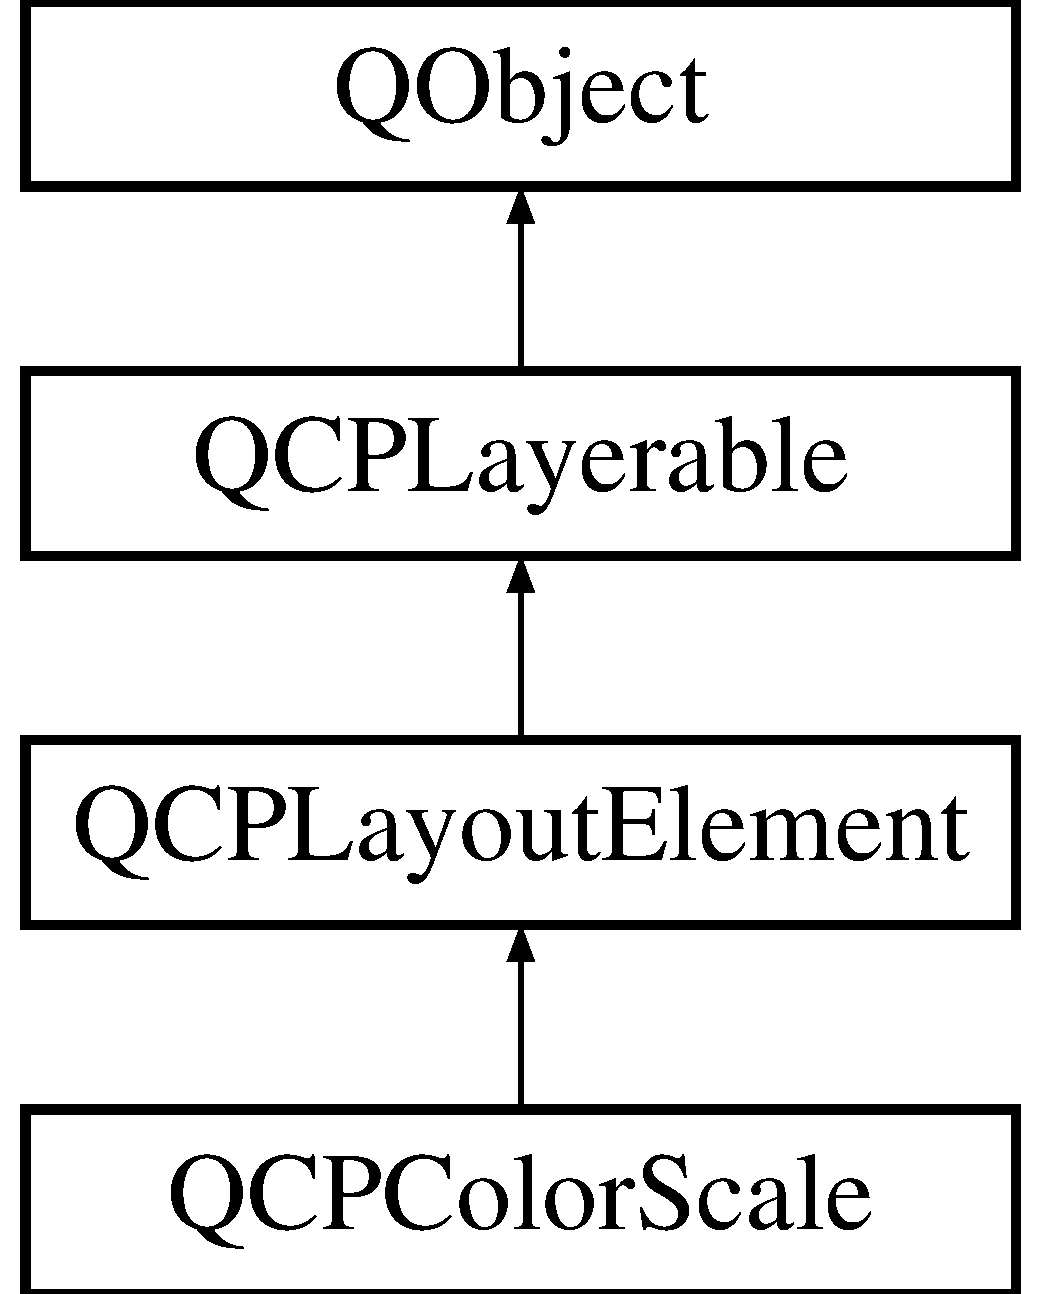
\includegraphics[height=4.000000cm]{class_q_c_p_color_scale}
\end{center}
\end{figure}
\subsection*{Signals}
\begin{DoxyCompactItemize}
\item 
void \hyperlink{class_q_c_p_color_scale_a293176da9447ec6819be1d901966a257}{data\+Range\+Changed} (\hyperlink{class_q_c_p_range}{Q\+C\+P\+Range} new\+Range)
\item 
void \hyperlink{class_q_c_p_color_scale_a61558b962f7791ff2f15a565dcf60181}{data\+Scale\+Type\+Changed} (\hyperlink{class_q_c_p_axis_a36d8e8658dbaa179bf2aeb973db2d6f0}{Q\+C\+P\+Axis\+::\+Scale\+Type} scale\+Type)
\item 
void \hyperlink{class_q_c_p_color_scale_a67a5eb06cf551d322885e8635a46378c}{gradient\+Changed} (\hyperlink{class_q_c_p_color_gradient}{Q\+C\+P\+Color\+Gradient} new\+Gradient)
\end{DoxyCompactItemize}
\subsection*{Public Member Functions}
\begin{DoxyCompactItemize}
\item 
\hyperlink{class_q_c_p_color_scale_aa8debce1be38b54287c04d4f584394b4}{Q\+C\+P\+Color\+Scale} (\hyperlink{class_q_custom_plot}{Q\+Custom\+Plot} $\ast$parent\+Plot)
\item 
\hyperlink{class_q_c_p_axis}{Q\+C\+P\+Axis} $\ast$ \hyperlink{class_q_c_p_color_scale_a39bdbdb3b212602a5a57f9f3ea444190}{axis} () const
\item 
\hypertarget{class_q_c_p_color_scale_a85d7e286fbfc0c04c4b480aff3cb66fb}{}\label{class_q_c_p_color_scale_a85d7e286fbfc0c04c4b480aff3cb66fb} 
\hyperlink{class_q_c_p_axis_ae2bcc1728b382f10f064612b368bc18a}{Q\+C\+P\+Axis\+::\+Axis\+Type} {\bfseries type} () const
\item 
\hypertarget{class_q_c_p_color_scale_a51f5756f99867bd91e570eddefeb1ef4}{}\label{class_q_c_p_color_scale_a51f5756f99867bd91e570eddefeb1ef4} 
\hyperlink{class_q_c_p_range}{Q\+C\+P\+Range} {\bfseries data\+Range} () const
\item 
\hypertarget{class_q_c_p_color_scale_ad864329d93cbd7396af1b2024db7fcfe}{}\label{class_q_c_p_color_scale_ad864329d93cbd7396af1b2024db7fcfe} 
\hyperlink{class_q_c_p_axis_a36d8e8658dbaa179bf2aeb973db2d6f0}{Q\+C\+P\+Axis\+::\+Scale\+Type} {\bfseries data\+Scale\+Type} () const
\item 
\hypertarget{class_q_c_p_color_scale_a31d4e3b49461bf6b265eabd028d0f7b2}{}\label{class_q_c_p_color_scale_a31d4e3b49461bf6b265eabd028d0f7b2} 
\hyperlink{class_q_c_p_color_gradient}{Q\+C\+P\+Color\+Gradient} {\bfseries gradient} () const
\item 
\hypertarget{class_q_c_p_color_scale_a3dbac1121a90172d62f01ab80b1ad641}{}\label{class_q_c_p_color_scale_a3dbac1121a90172d62f01ab80b1ad641} 
Q\+String {\bfseries label} () const
\item 
\hypertarget{class_q_c_p_color_scale_ae02ab8e4bfaa919577992e73242f491f}{}\label{class_q_c_p_color_scale_ae02ab8e4bfaa919577992e73242f491f} 
int {\bfseries bar\+Width} () const
\item 
\hypertarget{class_q_c_p_color_scale_a2a0670492f2a780596ea455ea8496a78}{}\label{class_q_c_p_color_scale_a2a0670492f2a780596ea455ea8496a78} 
bool {\bfseries range\+Drag} () const
\item 
\hypertarget{class_q_c_p_color_scale_adb4c3ada2b1e5ebbdead3b097064ff0b}{}\label{class_q_c_p_color_scale_adb4c3ada2b1e5ebbdead3b097064ff0b} 
bool {\bfseries range\+Zoom} () const
\item 
void \hyperlink{class_q_c_p_color_scale_a1bf9bdb291927c422dd66b404b206f1f}{set\+Type} (\hyperlink{class_q_c_p_axis_ae2bcc1728b382f10f064612b368bc18a}{Q\+C\+P\+Axis\+::\+Axis\+Type} type)
\item 
Q\+\_\+\+S\+L\+OT void \hyperlink{class_q_c_p_color_scale_abe88633003a26d1e756aa74984587fef}{set\+Data\+Range} (const \hyperlink{class_q_c_p_range}{Q\+C\+P\+Range} \&data\+Range)
\item 
Q\+\_\+\+S\+L\+OT void \hyperlink{class_q_c_p_color_scale_aeb6107d67dd7325145b2498abae67fc3}{set\+Data\+Scale\+Type} (\hyperlink{class_q_c_p_axis_a36d8e8658dbaa179bf2aeb973db2d6f0}{Q\+C\+P\+Axis\+::\+Scale\+Type} scale\+Type)
\item 
Q\+\_\+\+S\+L\+OT void \hyperlink{class_q_c_p_color_scale_a1f29583bb6f1e7f473b62fb712be3940}{set\+Gradient} (const \hyperlink{class_q_c_p_color_gradient}{Q\+C\+P\+Color\+Gradient} \&gradient)
\item 
void \hyperlink{class_q_c_p_color_scale_aee124ae8396320cacf8276e9a0fbb8ce}{set\+Label} (const Q\+String \&str)
\item 
void \hyperlink{class_q_c_p_color_scale_ab9dcc0c1cd583477496209b1413bcb99}{set\+Bar\+Width} (int width)
\item 
void \hyperlink{class_q_c_p_color_scale_a21c51a55e4fd581b6feadca9ee5b38d5}{set\+Range\+Drag} (bool enabled)
\item 
void \hyperlink{class_q_c_p_color_scale_a96bd60fb6317ad6821841b539c93eeeb}{set\+Range\+Zoom} (bool enabled)
\item 
Q\+List$<$ \hyperlink{class_q_c_p_color_map}{Q\+C\+P\+Color\+Map} $\ast$ $>$ \hyperlink{class_q_c_p_color_scale_a556adc6b0216ebc1cc4317c541956d06}{color\+Maps} () const
\item 
void \hyperlink{class_q_c_p_color_scale_a425983db4478543924ddbd04ea20a356}{rescale\+Data\+Range} (bool only\+Visible\+Maps)
\item 
virtual void \hyperlink{class_q_c_p_color_scale_ab8f6991ac88243fc582b44b183670334}{update} (\hyperlink{class_q_c_p_layout_element_a0d83360e05735735aaf6d7983c56374d}{Update\+Phase} phase)
\end{DoxyCompactItemize}
\subsection*{Protected Member Functions}
\begin{DoxyCompactItemize}
\item 
\hypertarget{class_q_c_p_color_scale_adcd2fa0d7f53d73788ec1cf54e44a6e2}{}\label{class_q_c_p_color_scale_adcd2fa0d7f53d73788ec1cf54e44a6e2} 
virtual void {\bfseries apply\+Default\+Antialiasing\+Hint} (\hyperlink{class_q_c_p_painter}{Q\+C\+P\+Painter} $\ast$painter) const
\item 
virtual void \hyperlink{class_q_c_p_color_scale_a5df6ad81b2ad045878d276c2d5be7120}{mouse\+Press\+Event} (Q\+Mouse\+Event $\ast$event)
\item 
virtual void \hyperlink{class_q_c_p_color_scale_a3aca469d531ce7b5882de73590aa0de6}{mouse\+Move\+Event} (Q\+Mouse\+Event $\ast$event)
\item 
virtual void \hyperlink{class_q_c_p_color_scale_a0916613d20901950fc6d00c6f99fe0a1}{mouse\+Release\+Event} (Q\+Mouse\+Event $\ast$event)
\item 
virtual void \hyperlink{class_q_c_p_color_scale_ab398e14c01240f3dc855884fe9e1ee8c}{wheel\+Event} (Q\+Wheel\+Event $\ast$event)
\end{DoxyCompactItemize}
\subsection*{Protected Attributes}
\begin{DoxyCompactItemize}
\item 
\hypertarget{class_q_c_p_color_scale_a7d47ed4ab76f38e50164e9d77fe33789}{}\label{class_q_c_p_color_scale_a7d47ed4ab76f38e50164e9d77fe33789} 
\hyperlink{class_q_c_p_axis_ae2bcc1728b382f10f064612b368bc18a}{Q\+C\+P\+Axis\+::\+Axis\+Type} {\bfseries m\+Type}
\item 
\hypertarget{class_q_c_p_color_scale_a5d4853feb32cd0077bb2b871687c844b}{}\label{class_q_c_p_color_scale_a5d4853feb32cd0077bb2b871687c844b} 
\hyperlink{class_q_c_p_range}{Q\+C\+P\+Range} {\bfseries m\+Data\+Range}
\item 
\hypertarget{class_q_c_p_color_scale_a2754d6a78736f64a241e333fbd955372}{}\label{class_q_c_p_color_scale_a2754d6a78736f64a241e333fbd955372} 
\hyperlink{class_q_c_p_axis_a36d8e8658dbaa179bf2aeb973db2d6f0}{Q\+C\+P\+Axis\+::\+Scale\+Type} {\bfseries m\+Data\+Scale\+Type}
\item 
\hypertarget{class_q_c_p_color_scale_ae195a385032066b5c46cc3301af58922}{}\label{class_q_c_p_color_scale_ae195a385032066b5c46cc3301af58922} 
\hyperlink{class_q_c_p_color_gradient}{Q\+C\+P\+Color\+Gradient} {\bfseries m\+Gradient}
\item 
\hypertarget{class_q_c_p_color_scale_a409d2ab78dff1f92da5e6acfb062e811}{}\label{class_q_c_p_color_scale_a409d2ab78dff1f92da5e6acfb062e811} 
int {\bfseries m\+Bar\+Width}
\item 
\hypertarget{class_q_c_p_color_scale_a6e37f7d49cd614dc50ef1caae60461b9}{}\label{class_q_c_p_color_scale_a6e37f7d49cd614dc50ef1caae60461b9} 
Q\+Pointer$<$ \hyperlink{class_q_c_p_color_scale_axis_rect_private}{Q\+C\+P\+Color\+Scale\+Axis\+Rect\+Private} $>$ {\bfseries m\+Axis\+Rect}
\item 
\hypertarget{class_q_c_p_color_scale_a2efbc90fd31898fe05d2b74a8422b1d5}{}\label{class_q_c_p_color_scale_a2efbc90fd31898fe05d2b74a8422b1d5} 
Q\+Pointer$<$ \hyperlink{class_q_c_p_axis}{Q\+C\+P\+Axis} $>$ {\bfseries m\+Color\+Axis}
\end{DoxyCompactItemize}
\subsection*{Friends}
\begin{DoxyCompactItemize}
\item 
\hypertarget{class_q_c_p_color_scale_a1441d8c09d7227c0c29a8d0a96d55bfe}{}\label{class_q_c_p_color_scale_a1441d8c09d7227c0c29a8d0a96d55bfe} 
class {\bfseries Q\+C\+P\+Color\+Scale\+Axis\+Rect\+Private}
\end{DoxyCompactItemize}
\subsection*{Additional Inherited Members}


\subsection{Detailed Description}
A color scale for use with color coding data such as \hyperlink{class_q_c_p_color_map}{Q\+C\+P\+Color\+Map}. 

This layout element can be placed on the plot to correlate a color gradient with data values. It is usually used in combination with one or multiple \hyperlink{class_q_c_p_color_map}{Q\+C\+P\+Color\+Maps}.



The color scale can be either horizontal or vertical, as shown in the image above. The orientation and the side where the numbers appear is controlled with \hyperlink{class_q_c_p_color_scale_a1bf9bdb291927c422dd66b404b206f1f}{set\+Type}.

Use \hyperlink{class_q_c_p_color_map_aa828921db364fe3c6af4619580ab85fd}{Q\+C\+P\+Color\+Map\+::set\+Color\+Scale} to connect a color map with a color scale. Once they are connected, they share their gradient, data range and data scale type (\hyperlink{class_q_c_p_color_scale_a1f29583bb6f1e7f473b62fb712be3940}{set\+Gradient}, \hyperlink{class_q_c_p_color_scale_abe88633003a26d1e756aa74984587fef}{set\+Data\+Range}, \hyperlink{class_q_c_p_color_scale_aeb6107d67dd7325145b2498abae67fc3}{set\+Data\+Scale\+Type}). Multiple color maps may be associated with a single color scale, to make them all synchronize these properties.

To have finer control over the number display and axis behaviour, you can directly access the \hyperlink{class_q_c_p_color_scale_a39bdbdb3b212602a5a57f9f3ea444190}{axis}. See the documentation of \hyperlink{class_q_c_p_axis}{Q\+C\+P\+Axis} for details about configuring axes. For example, if you want to change the number of automatically generated ticks, call 
\begin{DoxyCodeInclude}
\end{DoxyCodeInclude}
 Placing a color scale next to the main axis rect works like with any other layout element\+: 
\begin{DoxyCodeInclude}
\end{DoxyCodeInclude}
In this case we have placed it to the right of the default axis rect, so it wasn\textquotesingle{}t necessary to call \hyperlink{class_q_c_p_color_scale_a1bf9bdb291927c422dd66b404b206f1f}{set\+Type}, since \hyperlink{class_q_c_p_axis_ae2bcc1728b382f10f064612b368bc18aadf5509f7d29199ef2f263b1dd224b345}{Q\+C\+P\+Axis\+::at\+Right} is already the default. The text next to the color scale can be set with \hyperlink{class_q_c_p_color_scale_aee124ae8396320cacf8276e9a0fbb8ce}{set\+Label}.

For optimum appearance (like in the image above), it may be desirable to line up the axis rect and the borders of the color scale. Use a \hyperlink{class_q_c_p_margin_group}{Q\+C\+P\+Margin\+Group} to achieve this\+: 
\begin{DoxyCodeInclude}
\end{DoxyCodeInclude}
 Color scales are initialized with a non-\/zero minimum top and bottom margin (\hyperlink{class_q_c_p_layout_element_a0a8a17abc16b7923159fcc7608f94673}{set\+Minimum\+Margins}), because vertical color scales are most common and the minimum top/bottom margin makes sure it keeps some distance to the top/bottom widget border. So if you change to a horizontal color scale by setting \hyperlink{class_q_c_p_color_scale_a1bf9bdb291927c422dd66b404b206f1f}{set\+Type} to \hyperlink{class_q_c_p_axis_ae2bcc1728b382f10f064612b368bc18aa220d68888516b6c3b493d144f1ba438f}{Q\+C\+P\+Axis\+::at\+Bottom} or \hyperlink{class_q_c_p_axis_ae2bcc1728b382f10f064612b368bc18aac0ece2b680d3f545e701f75af1655977}{Q\+C\+P\+Axis\+::at\+Top}, you might want to also change the minimum margins accordingly, e.\+g. {\ttfamily set\+Minimum\+Margins(\+Q\+Margins(6, 0, 6, 0))}. 

\subsection{Constructor \& Destructor Documentation}
\hypertarget{class_q_c_p_color_scale_aa8debce1be38b54287c04d4f584394b4}{}\label{class_q_c_p_color_scale_aa8debce1be38b54287c04d4f584394b4} 
\index{Q\+C\+P\+Color\+Scale@{Q\+C\+P\+Color\+Scale}!Q\+C\+P\+Color\+Scale@{Q\+C\+P\+Color\+Scale}}
\index{Q\+C\+P\+Color\+Scale@{Q\+C\+P\+Color\+Scale}!Q\+C\+P\+Color\+Scale@{Q\+C\+P\+Color\+Scale}}
\subsubsection{\texorpdfstring{Q\+C\+P\+Color\+Scale()}{QCPColorScale()}}
{\footnotesize\ttfamily Q\+C\+P\+Color\+Scale\+::\+Q\+C\+P\+Color\+Scale (\begin{DoxyParamCaption}\item[{\hyperlink{class_q_custom_plot}{Q\+Custom\+Plot} $\ast$}]{parent\+Plot }\end{DoxyParamCaption})\hspace{0.3cm}{\ttfamily [explicit]}}

Constructs a new \hyperlink{class_q_c_p_color_scale}{Q\+C\+P\+Color\+Scale}. 

\subsection{Member Function Documentation}
\hypertarget{class_q_c_p_color_scale_a39bdbdb3b212602a5a57f9f3ea444190}{}\label{class_q_c_p_color_scale_a39bdbdb3b212602a5a57f9f3ea444190} 
\index{Q\+C\+P\+Color\+Scale@{Q\+C\+P\+Color\+Scale}!axis@{axis}}
\index{axis@{axis}!Q\+C\+P\+Color\+Scale@{Q\+C\+P\+Color\+Scale}}
\subsubsection{\texorpdfstring{axis()}{axis()}}
{\footnotesize\ttfamily \hyperlink{class_q_c_p_axis}{Q\+C\+P\+Axis} $\ast$ Q\+C\+P\+Color\+Scale\+::axis (\begin{DoxyParamCaption}{ }\end{DoxyParamCaption}) const\hspace{0.3cm}{\ttfamily [inline]}}

Returns the internal \hyperlink{class_q_c_p_axis}{Q\+C\+P\+Axis} instance of this color scale. You can access it to alter the appearance and behaviour of the axis. \hyperlink{class_q_c_p_color_scale}{Q\+C\+P\+Color\+Scale} duplicates some properties in its interface for convenience. Those are \hyperlink{class_q_c_p_color_scale_abe88633003a26d1e756aa74984587fef}{set\+Data\+Range} (\hyperlink{class_q_c_p_axis_aebdfea5d44c3a0ad2b4700cd4d25b641}{Q\+C\+P\+Axis\+::set\+Range}), \hyperlink{class_q_c_p_color_scale_aeb6107d67dd7325145b2498abae67fc3}{set\+Data\+Scale\+Type} (\hyperlink{class_q_c_p_axis_adef29cae617af4f519f6c40d1a866ca6}{Q\+C\+P\+Axis\+::set\+Scale\+Type}), and the method \hyperlink{class_q_c_p_color_scale_aee124ae8396320cacf8276e9a0fbb8ce}{set\+Label} (\hyperlink{class_q_c_p_axis_a33bcc382c111c9f31bb0687352a2dea4}{Q\+C\+P\+Axis\+::set\+Label}). As they each are connected, it does not matter whether you use the method on the \hyperlink{class_q_c_p_color_scale}{Q\+C\+P\+Color\+Scale} or on its \hyperlink{class_q_c_p_axis}{Q\+C\+P\+Axis}.

If the type of the color scale is changed with \hyperlink{class_q_c_p_color_scale_a1bf9bdb291927c422dd66b404b206f1f}{set\+Type}, the axis returned by this method will change, too, to either the left, right, bottom or top axis, depending on which type was set. \hypertarget{class_q_c_p_color_scale_a556adc6b0216ebc1cc4317c541956d06}{}\label{class_q_c_p_color_scale_a556adc6b0216ebc1cc4317c541956d06} 
\index{Q\+C\+P\+Color\+Scale@{Q\+C\+P\+Color\+Scale}!color\+Maps@{color\+Maps}}
\index{color\+Maps@{color\+Maps}!Q\+C\+P\+Color\+Scale@{Q\+C\+P\+Color\+Scale}}
\subsubsection{\texorpdfstring{color\+Maps()}{colorMaps()}}
{\footnotesize\ttfamily Q\+List$<$ \hyperlink{class_q_c_p_color_map}{Q\+C\+P\+Color\+Map} $\ast$ $>$ Q\+C\+P\+Color\+Scale\+::color\+Maps (\begin{DoxyParamCaption}{ }\end{DoxyParamCaption}) const}

Returns a list of all the color maps associated with this color scale. \hypertarget{class_q_c_p_color_scale_a293176da9447ec6819be1d901966a257}{}\label{class_q_c_p_color_scale_a293176da9447ec6819be1d901966a257} 
\index{Q\+C\+P\+Color\+Scale@{Q\+C\+P\+Color\+Scale}!data\+Range\+Changed@{data\+Range\+Changed}}
\index{data\+Range\+Changed@{data\+Range\+Changed}!Q\+C\+P\+Color\+Scale@{Q\+C\+P\+Color\+Scale}}
\subsubsection{\texorpdfstring{data\+Range\+Changed}{dataRangeChanged}}
{\footnotesize\ttfamily void Q\+C\+P\+Color\+Scale\+::data\+Range\+Changed (\begin{DoxyParamCaption}\item[{\hyperlink{class_q_c_p_range}{Q\+C\+P\+Range}}]{new\+Range }\end{DoxyParamCaption})\hspace{0.3cm}{\ttfamily [signal]}}

This signal is emitted when the data range changes.

\begin{DoxySeeAlso}{See also}
\hyperlink{class_q_c_p_color_scale_abe88633003a26d1e756aa74984587fef}{set\+Data\+Range} 
\end{DoxySeeAlso}
\hypertarget{class_q_c_p_color_scale_a61558b962f7791ff2f15a565dcf60181}{}\label{class_q_c_p_color_scale_a61558b962f7791ff2f15a565dcf60181} 
\index{Q\+C\+P\+Color\+Scale@{Q\+C\+P\+Color\+Scale}!data\+Scale\+Type\+Changed@{data\+Scale\+Type\+Changed}}
\index{data\+Scale\+Type\+Changed@{data\+Scale\+Type\+Changed}!Q\+C\+P\+Color\+Scale@{Q\+C\+P\+Color\+Scale}}
\subsubsection{\texorpdfstring{data\+Scale\+Type\+Changed}{dataScaleTypeChanged}}
{\footnotesize\ttfamily void Q\+C\+P\+Color\+Scale\+::data\+Scale\+Type\+Changed (\begin{DoxyParamCaption}\item[{\hyperlink{class_q_c_p_axis_a36d8e8658dbaa179bf2aeb973db2d6f0}{Q\+C\+P\+Axis\+::\+Scale\+Type}}]{scale\+Type }\end{DoxyParamCaption})\hspace{0.3cm}{\ttfamily [signal]}}

This signal is emitted when the data scale type changes.

\begin{DoxySeeAlso}{See also}
\hyperlink{class_q_c_p_color_scale_aeb6107d67dd7325145b2498abae67fc3}{set\+Data\+Scale\+Type} 
\end{DoxySeeAlso}
\hypertarget{class_q_c_p_color_scale_a67a5eb06cf551d322885e8635a46378c}{}\label{class_q_c_p_color_scale_a67a5eb06cf551d322885e8635a46378c} 
\index{Q\+C\+P\+Color\+Scale@{Q\+C\+P\+Color\+Scale}!gradient\+Changed@{gradient\+Changed}}
\index{gradient\+Changed@{gradient\+Changed}!Q\+C\+P\+Color\+Scale@{Q\+C\+P\+Color\+Scale}}
\subsubsection{\texorpdfstring{gradient\+Changed}{gradientChanged}}
{\footnotesize\ttfamily void Q\+C\+P\+Color\+Scale\+::gradient\+Changed (\begin{DoxyParamCaption}\item[{\hyperlink{class_q_c_p_color_gradient}{Q\+C\+P\+Color\+Gradient}}]{new\+Gradient }\end{DoxyParamCaption})\hspace{0.3cm}{\ttfamily [signal]}}

This signal is emitted when the gradient changes.

\begin{DoxySeeAlso}{See also}
\hyperlink{class_q_c_p_color_scale_a1f29583bb6f1e7f473b62fb712be3940}{set\+Gradient} 
\end{DoxySeeAlso}
\hypertarget{class_q_c_p_color_scale_a3aca469d531ce7b5882de73590aa0de6}{}\label{class_q_c_p_color_scale_a3aca469d531ce7b5882de73590aa0de6} 
\index{Q\+C\+P\+Color\+Scale@{Q\+C\+P\+Color\+Scale}!mouse\+Move\+Event@{mouse\+Move\+Event}}
\index{mouse\+Move\+Event@{mouse\+Move\+Event}!Q\+C\+P\+Color\+Scale@{Q\+C\+P\+Color\+Scale}}
\subsubsection{\texorpdfstring{mouse\+Move\+Event()}{mouseMoveEvent()}}
{\footnotesize\ttfamily void Q\+C\+P\+Color\+Scale\+::mouse\+Move\+Event (\begin{DoxyParamCaption}\item[{Q\+Mouse\+Event $\ast$}]{event }\end{DoxyParamCaption})\hspace{0.3cm}{\ttfamily [protected]}, {\ttfamily [virtual]}}

This event is called, if the mouse is moved inside the outer rect of this layout element. 

Reimplemented from \hyperlink{class_q_c_p_layout_element_a14f4acf58cdb8dd2c6c571479c4c4a40}{Q\+C\+P\+Layout\+Element}.

\hypertarget{class_q_c_p_color_scale_a5df6ad81b2ad045878d276c2d5be7120}{}\label{class_q_c_p_color_scale_a5df6ad81b2ad045878d276c2d5be7120} 
\index{Q\+C\+P\+Color\+Scale@{Q\+C\+P\+Color\+Scale}!mouse\+Press\+Event@{mouse\+Press\+Event}}
\index{mouse\+Press\+Event@{mouse\+Press\+Event}!Q\+C\+P\+Color\+Scale@{Q\+C\+P\+Color\+Scale}}
\subsubsection{\texorpdfstring{mouse\+Press\+Event()}{mousePressEvent()}}
{\footnotesize\ttfamily void Q\+C\+P\+Color\+Scale\+::mouse\+Press\+Event (\begin{DoxyParamCaption}\item[{Q\+Mouse\+Event $\ast$}]{event }\end{DoxyParamCaption})\hspace{0.3cm}{\ttfamily [protected]}, {\ttfamily [virtual]}}

This event is called, if the mouse was pressed while being inside the outer rect of this layout element. 

Reimplemented from \hyperlink{class_q_c_p_layout_element_a2d82ea21fe0ee628f177bd824bc51a71}{Q\+C\+P\+Layout\+Element}.

\hypertarget{class_q_c_p_color_scale_a0916613d20901950fc6d00c6f99fe0a1}{}\label{class_q_c_p_color_scale_a0916613d20901950fc6d00c6f99fe0a1} 
\index{Q\+C\+P\+Color\+Scale@{Q\+C\+P\+Color\+Scale}!mouse\+Release\+Event@{mouse\+Release\+Event}}
\index{mouse\+Release\+Event@{mouse\+Release\+Event}!Q\+C\+P\+Color\+Scale@{Q\+C\+P\+Color\+Scale}}
\subsubsection{\texorpdfstring{mouse\+Release\+Event()}{mouseReleaseEvent()}}
{\footnotesize\ttfamily void Q\+C\+P\+Color\+Scale\+::mouse\+Release\+Event (\begin{DoxyParamCaption}\item[{Q\+Mouse\+Event $\ast$}]{event }\end{DoxyParamCaption})\hspace{0.3cm}{\ttfamily [protected]}, {\ttfamily [virtual]}}

This event is called, if the mouse was previously pressed inside the outer rect of this layout element and is now released. 

Reimplemented from \hyperlink{class_q_c_p_layout_element_ae526ac828cce1e5bb94eaa85776d7404}{Q\+C\+P\+Layout\+Element}.

\hypertarget{class_q_c_p_color_scale_a425983db4478543924ddbd04ea20a356}{}\label{class_q_c_p_color_scale_a425983db4478543924ddbd04ea20a356} 
\index{Q\+C\+P\+Color\+Scale@{Q\+C\+P\+Color\+Scale}!rescale\+Data\+Range@{rescale\+Data\+Range}}
\index{rescale\+Data\+Range@{rescale\+Data\+Range}!Q\+C\+P\+Color\+Scale@{Q\+C\+P\+Color\+Scale}}
\subsubsection{\texorpdfstring{rescale\+Data\+Range()}{rescaleDataRange()}}
{\footnotesize\ttfamily void Q\+C\+P\+Color\+Scale\+::rescale\+Data\+Range (\begin{DoxyParamCaption}\item[{bool}]{only\+Visible\+Maps }\end{DoxyParamCaption})}

Changes the data range such that all color maps associated with this color scale are fully mapped to the gradient in the data dimension.

\begin{DoxySeeAlso}{See also}
\hyperlink{class_q_c_p_color_scale_abe88633003a26d1e756aa74984587fef}{set\+Data\+Range} 
\end{DoxySeeAlso}
\hypertarget{class_q_c_p_color_scale_ab9dcc0c1cd583477496209b1413bcb99}{}\label{class_q_c_p_color_scale_ab9dcc0c1cd583477496209b1413bcb99} 
\index{Q\+C\+P\+Color\+Scale@{Q\+C\+P\+Color\+Scale}!set\+Bar\+Width@{set\+Bar\+Width}}
\index{set\+Bar\+Width@{set\+Bar\+Width}!Q\+C\+P\+Color\+Scale@{Q\+C\+P\+Color\+Scale}}
\subsubsection{\texorpdfstring{set\+Bar\+Width()}{setBarWidth()}}
{\footnotesize\ttfamily void Q\+C\+P\+Color\+Scale\+::set\+Bar\+Width (\begin{DoxyParamCaption}\item[{int}]{width }\end{DoxyParamCaption})}

Sets the width (or height, for horizontal color scales) the bar where the gradient is displayed will have. \hypertarget{class_q_c_p_color_scale_abe88633003a26d1e756aa74984587fef}{}\label{class_q_c_p_color_scale_abe88633003a26d1e756aa74984587fef} 
\index{Q\+C\+P\+Color\+Scale@{Q\+C\+P\+Color\+Scale}!set\+Data\+Range@{set\+Data\+Range}}
\index{set\+Data\+Range@{set\+Data\+Range}!Q\+C\+P\+Color\+Scale@{Q\+C\+P\+Color\+Scale}}
\subsubsection{\texorpdfstring{set\+Data\+Range()}{setDataRange()}}
{\footnotesize\ttfamily void Q\+C\+P\+Color\+Scale\+::set\+Data\+Range (\begin{DoxyParamCaption}\item[{const \hyperlink{class_q_c_p_range}{Q\+C\+P\+Range} \&}]{data\+Range }\end{DoxyParamCaption})}

Sets the range spanned by the color gradient and that is shown by the axis in the color scale.

It is equivalent to calling \hyperlink{class_q_c_p_color_map_a980b42837821159786a85b4b7dcb8774}{Q\+C\+P\+Color\+Map\+::set\+Data\+Range} on any of the connected color maps. It is also equivalent to directly accessing the \hyperlink{class_q_c_p_color_scale_a39bdbdb3b212602a5a57f9f3ea444190}{axis} and setting its range with \hyperlink{class_q_c_p_axis_aebdfea5d44c3a0ad2b4700cd4d25b641}{Q\+C\+P\+Axis\+::set\+Range}.

\begin{DoxySeeAlso}{See also}
\hyperlink{class_q_c_p_color_scale_aeb6107d67dd7325145b2498abae67fc3}{set\+Data\+Scale\+Type}, \hyperlink{class_q_c_p_color_scale_a1f29583bb6f1e7f473b62fb712be3940}{set\+Gradient}, \hyperlink{class_q_c_p_color_scale_a425983db4478543924ddbd04ea20a356}{rescale\+Data\+Range} 
\end{DoxySeeAlso}
\hypertarget{class_q_c_p_color_scale_aeb6107d67dd7325145b2498abae67fc3}{}\label{class_q_c_p_color_scale_aeb6107d67dd7325145b2498abae67fc3} 
\index{Q\+C\+P\+Color\+Scale@{Q\+C\+P\+Color\+Scale}!set\+Data\+Scale\+Type@{set\+Data\+Scale\+Type}}
\index{set\+Data\+Scale\+Type@{set\+Data\+Scale\+Type}!Q\+C\+P\+Color\+Scale@{Q\+C\+P\+Color\+Scale}}
\subsubsection{\texorpdfstring{set\+Data\+Scale\+Type()}{setDataScaleType()}}
{\footnotesize\ttfamily void Q\+C\+P\+Color\+Scale\+::set\+Data\+Scale\+Type (\begin{DoxyParamCaption}\item[{\hyperlink{class_q_c_p_axis_a36d8e8658dbaa179bf2aeb973db2d6f0}{Q\+C\+P\+Axis\+::\+Scale\+Type}}]{scale\+Type }\end{DoxyParamCaption})}

Sets the scale type of the color scale, i.\+e. whether values are linearly associated with colors or logarithmically.

It is equivalent to calling \hyperlink{class_q_c_p_color_map_a9d20aa08e3c1f20f22908c45b9c06511}{Q\+C\+P\+Color\+Map\+::set\+Data\+Scale\+Type} on any of the connected color maps. It is also equivalent to directly accessing the \hyperlink{class_q_c_p_color_scale_a39bdbdb3b212602a5a57f9f3ea444190}{axis} and setting its scale type with \hyperlink{class_q_c_p_axis_adef29cae617af4f519f6c40d1a866ca6}{Q\+C\+P\+Axis\+::set\+Scale\+Type}.

\begin{DoxySeeAlso}{See also}
\hyperlink{class_q_c_p_color_scale_abe88633003a26d1e756aa74984587fef}{set\+Data\+Range}, \hyperlink{class_q_c_p_color_scale_a1f29583bb6f1e7f473b62fb712be3940}{set\+Gradient} 
\end{DoxySeeAlso}
\hypertarget{class_q_c_p_color_scale_a1f29583bb6f1e7f473b62fb712be3940}{}\label{class_q_c_p_color_scale_a1f29583bb6f1e7f473b62fb712be3940} 
\index{Q\+C\+P\+Color\+Scale@{Q\+C\+P\+Color\+Scale}!set\+Gradient@{set\+Gradient}}
\index{set\+Gradient@{set\+Gradient}!Q\+C\+P\+Color\+Scale@{Q\+C\+P\+Color\+Scale}}
\subsubsection{\texorpdfstring{set\+Gradient()}{setGradient()}}
{\footnotesize\ttfamily void Q\+C\+P\+Color\+Scale\+::set\+Gradient (\begin{DoxyParamCaption}\item[{const \hyperlink{class_q_c_p_color_gradient}{Q\+C\+P\+Color\+Gradient} \&}]{gradient }\end{DoxyParamCaption})}

Sets the color gradient that will be used to represent data values.

It is equivalent to calling \hyperlink{class_q_c_p_color_map_a7313c78360471cead3576341a2c50377}{Q\+C\+P\+Color\+Map\+::set\+Gradient} on any of the connected color maps.

\begin{DoxySeeAlso}{See also}
\hyperlink{class_q_c_p_color_scale_abe88633003a26d1e756aa74984587fef}{set\+Data\+Range}, \hyperlink{class_q_c_p_color_scale_aeb6107d67dd7325145b2498abae67fc3}{set\+Data\+Scale\+Type} 
\end{DoxySeeAlso}
\hypertarget{class_q_c_p_color_scale_aee124ae8396320cacf8276e9a0fbb8ce}{}\label{class_q_c_p_color_scale_aee124ae8396320cacf8276e9a0fbb8ce} 
\index{Q\+C\+P\+Color\+Scale@{Q\+C\+P\+Color\+Scale}!set\+Label@{set\+Label}}
\index{set\+Label@{set\+Label}!Q\+C\+P\+Color\+Scale@{Q\+C\+P\+Color\+Scale}}
\subsubsection{\texorpdfstring{set\+Label()}{setLabel()}}
{\footnotesize\ttfamily void Q\+C\+P\+Color\+Scale\+::set\+Label (\begin{DoxyParamCaption}\item[{const Q\+String \&}]{str }\end{DoxyParamCaption})}

Sets the axis label of the color scale. This is equivalent to calling \hyperlink{class_q_c_p_axis_a33bcc382c111c9f31bb0687352a2dea4}{Q\+C\+P\+Axis\+::set\+Label} on the internal \hyperlink{class_q_c_p_color_scale_a39bdbdb3b212602a5a57f9f3ea444190}{axis}. \hypertarget{class_q_c_p_color_scale_a21c51a55e4fd581b6feadca9ee5b38d5}{}\label{class_q_c_p_color_scale_a21c51a55e4fd581b6feadca9ee5b38d5} 
\index{Q\+C\+P\+Color\+Scale@{Q\+C\+P\+Color\+Scale}!set\+Range\+Drag@{set\+Range\+Drag}}
\index{set\+Range\+Drag@{set\+Range\+Drag}!Q\+C\+P\+Color\+Scale@{Q\+C\+P\+Color\+Scale}}
\subsubsection{\texorpdfstring{set\+Range\+Drag()}{setRangeDrag()}}
{\footnotesize\ttfamily void Q\+C\+P\+Color\+Scale\+::set\+Range\+Drag (\begin{DoxyParamCaption}\item[{bool}]{enabled }\end{DoxyParamCaption})}

Sets whether the user can drag the data range (\hyperlink{class_q_c_p_color_scale_abe88633003a26d1e756aa74984587fef}{set\+Data\+Range}).

Note that \hyperlink{namespace_q_c_p_a2ad6bb6281c7c2d593d4277b44c2b037a2c4432b9aceafb94000be8d1b589ef18}{Q\+C\+P\+::i\+Range\+Drag} must be in the \hyperlink{class_q_custom_plot}{Q\+Custom\+Plot}\textquotesingle{}s interactions (\hyperlink{class_q_custom_plot_a5ee1e2f6ae27419deca53e75907c27e5}{Q\+Custom\+Plot\+::set\+Interactions}) to allow range dragging. \hypertarget{class_q_c_p_color_scale_a96bd60fb6317ad6821841b539c93eeeb}{}\label{class_q_c_p_color_scale_a96bd60fb6317ad6821841b539c93eeeb} 
\index{Q\+C\+P\+Color\+Scale@{Q\+C\+P\+Color\+Scale}!set\+Range\+Zoom@{set\+Range\+Zoom}}
\index{set\+Range\+Zoom@{set\+Range\+Zoom}!Q\+C\+P\+Color\+Scale@{Q\+C\+P\+Color\+Scale}}
\subsubsection{\texorpdfstring{set\+Range\+Zoom()}{setRangeZoom()}}
{\footnotesize\ttfamily void Q\+C\+P\+Color\+Scale\+::set\+Range\+Zoom (\begin{DoxyParamCaption}\item[{bool}]{enabled }\end{DoxyParamCaption})}

Sets whether the user can zoom the data range (\hyperlink{class_q_c_p_color_scale_abe88633003a26d1e756aa74984587fef}{set\+Data\+Range}) by scrolling the mouse wheel.

Note that \hyperlink{namespace_q_c_p_a2ad6bb6281c7c2d593d4277b44c2b037abee1e94353525a636aeaf0ba32b72e14}{Q\+C\+P\+::i\+Range\+Zoom} must be in the \hyperlink{class_q_custom_plot}{Q\+Custom\+Plot}\textquotesingle{}s interactions (\hyperlink{class_q_custom_plot_a5ee1e2f6ae27419deca53e75907c27e5}{Q\+Custom\+Plot\+::set\+Interactions}) to allow range dragging. \hypertarget{class_q_c_p_color_scale_a1bf9bdb291927c422dd66b404b206f1f}{}\label{class_q_c_p_color_scale_a1bf9bdb291927c422dd66b404b206f1f} 
\index{Q\+C\+P\+Color\+Scale@{Q\+C\+P\+Color\+Scale}!set\+Type@{set\+Type}}
\index{set\+Type@{set\+Type}!Q\+C\+P\+Color\+Scale@{Q\+C\+P\+Color\+Scale}}
\subsubsection{\texorpdfstring{set\+Type()}{setType()}}
{\footnotesize\ttfamily void Q\+C\+P\+Color\+Scale\+::set\+Type (\begin{DoxyParamCaption}\item[{\hyperlink{class_q_c_p_axis_ae2bcc1728b382f10f064612b368bc18a}{Q\+C\+P\+Axis\+::\+Axis\+Type}}]{type }\end{DoxyParamCaption})}

Sets at which side of the color scale the axis is placed, and thus also its orientation.

Note that after setting {\itshape type} to a different value, the axis returned by \hyperlink{class_q_c_p_color_scale_a39bdbdb3b212602a5a57f9f3ea444190}{axis()} will be a different one. The new axis will adopt the following properties from the previous axis\+: The range, scale type, log base and label. \hypertarget{class_q_c_p_color_scale_ab8f6991ac88243fc582b44b183670334}{}\label{class_q_c_p_color_scale_ab8f6991ac88243fc582b44b183670334} 
\index{Q\+C\+P\+Color\+Scale@{Q\+C\+P\+Color\+Scale}!update@{update}}
\index{update@{update}!Q\+C\+P\+Color\+Scale@{Q\+C\+P\+Color\+Scale}}
\subsubsection{\texorpdfstring{update()}{update()}}
{\footnotesize\ttfamily void Q\+C\+P\+Color\+Scale\+::update (\begin{DoxyParamCaption}\item[{\hyperlink{class_q_c_p_layout_element_a0d83360e05735735aaf6d7983c56374d}{Update\+Phase}}]{phase }\end{DoxyParamCaption})\hspace{0.3cm}{\ttfamily [virtual]}}

Updates the layout element and sub-\/elements. This function is automatically called before every replot by the parent layout element. It is called multiple times, once for every \hyperlink{class_q_c_p_layout_element_a0d83360e05735735aaf6d7983c56374d}{Update\+Phase}. The phases are run through in the order of the enum values. For details about what happens at the different phases, see the documentation of \hyperlink{class_q_c_p_layout_element_a0d83360e05735735aaf6d7983c56374d}{Update\+Phase}.

Layout elements that have child elements should call the \hyperlink{class_q_c_p_color_scale_ab8f6991ac88243fc582b44b183670334}{update} method of their child elements, and pass the current {\itshape phase} unchanged.

The default implementation executes the automatic margin mechanism in the \hyperlink{class_q_c_p_layout_element_a0d83360e05735735aaf6d7983c56374da288cb59a92280e47261a341f2813e676}{up\+Margins} phase. Subclasses should make sure to call the base class implementation. 

Reimplemented from \hyperlink{class_q_c_p_layout_element_a929c2ec62e0e0e1d8418eaa802e2af9b}{Q\+C\+P\+Layout\+Element}.

\hypertarget{class_q_c_p_color_scale_ab398e14c01240f3dc855884fe9e1ee8c}{}\label{class_q_c_p_color_scale_ab398e14c01240f3dc855884fe9e1ee8c} 
\index{Q\+C\+P\+Color\+Scale@{Q\+C\+P\+Color\+Scale}!wheel\+Event@{wheel\+Event}}
\index{wheel\+Event@{wheel\+Event}!Q\+C\+P\+Color\+Scale@{Q\+C\+P\+Color\+Scale}}
\subsubsection{\texorpdfstring{wheel\+Event()}{wheelEvent()}}
{\footnotesize\ttfamily void Q\+C\+P\+Color\+Scale\+::wheel\+Event (\begin{DoxyParamCaption}\item[{Q\+Wheel\+Event $\ast$}]{event }\end{DoxyParamCaption})\hspace{0.3cm}{\ttfamily [protected]}, {\ttfamily [virtual]}}

This event is called, if the mouse wheel is scrolled while the cursor is inside the rect of this layout element. 

Reimplemented from \hyperlink{class_q_c_p_layout_element_a300521d2fd18a893c1b85f6be11ce2bf}{Q\+C\+P\+Layout\+Element}.



The documentation for this class was generated from the following files\+:\begin{DoxyCompactItemize}
\item 
C\+:/\+Users/\+Jesse Jutson/\+Documents/\+Git\+Hub/\+F\+E\+S\+S\+G\+U\+I/\+F\+E\+S\+S-\/\+G\+U\+I/\hyperlink{qcustomplot_8h}{qcustomplot.\+h}\item 
C\+:/\+Users/\+Jesse Jutson/\+Documents/\+Git\+Hub/\+F\+E\+S\+S\+G\+U\+I/\+F\+E\+S\+S-\/\+G\+U\+I/\hyperlink{qcustomplot_8cpp}{qcustomplot.\+cpp}\end{DoxyCompactItemize}

\hypertarget{class_q_c_p_color_scale_axis_rect_private}{}\section{Q\+C\+P\+Color\+Scale\+Axis\+Rect\+Private Class Reference}
\label{class_q_c_p_color_scale_axis_rect_private}\index{Q\+C\+P\+Color\+Scale\+Axis\+Rect\+Private@{Q\+C\+P\+Color\+Scale\+Axis\+Rect\+Private}}
Inheritance diagram for Q\+C\+P\+Color\+Scale\+Axis\+Rect\+Private\+:\begin{figure}[H]
\begin{center}
\leavevmode
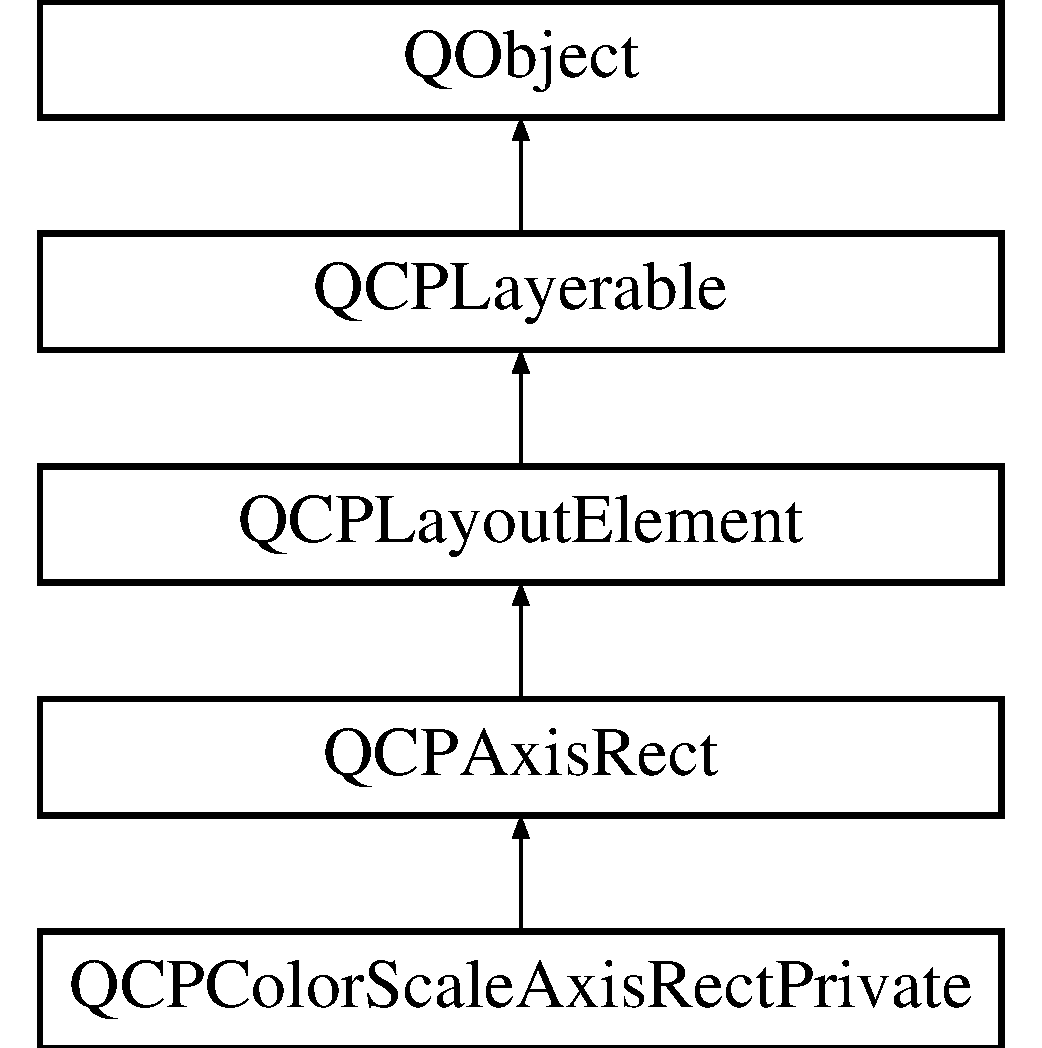
\includegraphics[height=5.000000cm]{class_q_c_p_color_scale_axis_rect_private}
\end{center}
\end{figure}
\subsection*{Public Member Functions}
\begin{DoxyCompactItemize}
\item 
\hyperlink{class_q_c_p_color_scale_axis_rect_private_ad3b242f75dd2b33581364a4e668a80db}{Q\+C\+P\+Color\+Scale\+Axis\+Rect\+Private} (\hyperlink{class_q_c_p_color_scale}{Q\+C\+P\+Color\+Scale} $\ast$parent\+Color\+Scale)
\end{DoxyCompactItemize}
\subsection*{Protected Member Functions}
\begin{DoxyCompactItemize}
\item 
\hypertarget{class_q_c_p_color_scale_axis_rect_private_adb67bfe9057a9dd9a85f548c274e6d98}{}\label{class_q_c_p_color_scale_axis_rect_private_adb67bfe9057a9dd9a85f548c274e6d98} 
virtual void {\bfseries draw} (\hyperlink{class_q_c_p_painter}{Q\+C\+P\+Painter} $\ast$painter)
\item 
\hypertarget{class_q_c_p_color_scale_axis_rect_private_a73754cab312aeaddea1bfcc67cc079ac}{}\label{class_q_c_p_color_scale_axis_rect_private_a73754cab312aeaddea1bfcc67cc079ac} 
void {\bfseries update\+Gradient\+Image} ()
\item 
\hypertarget{class_q_c_p_color_scale_axis_rect_private_a6112ad4291ac1695d37659cb049d598d}{}\label{class_q_c_p_color_scale_axis_rect_private_a6112ad4291ac1695d37659cb049d598d} 
Q\+\_\+\+S\+L\+OT void {\bfseries axis\+Selection\+Changed} (Q\+C\+P\+Axis\+::\+Selectable\+Parts selected\+Parts)
\item 
\hypertarget{class_q_c_p_color_scale_axis_rect_private_a66d2baed86966bb03a6d7c32dc7d59f7}{}\label{class_q_c_p_color_scale_axis_rect_private_a66d2baed86966bb03a6d7c32dc7d59f7} 
Q\+\_\+\+S\+L\+OT void {\bfseries axis\+Selectable\+Changed} (Q\+C\+P\+Axis\+::\+Selectable\+Parts selectable\+Parts)
\end{DoxyCompactItemize}
\subsection*{Protected Attributes}
\begin{DoxyCompactItemize}
\item 
\hypertarget{class_q_c_p_color_scale_axis_rect_private_a311c73f51a4cb0b556388197833cf099}{}\label{class_q_c_p_color_scale_axis_rect_private_a311c73f51a4cb0b556388197833cf099} 
\hyperlink{class_q_c_p_color_scale}{Q\+C\+P\+Color\+Scale} $\ast$ {\bfseries m\+Parent\+Color\+Scale}
\item 
\hypertarget{class_q_c_p_color_scale_axis_rect_private_ad4f7c8ee1c6012d9950870811773119c}{}\label{class_q_c_p_color_scale_axis_rect_private_ad4f7c8ee1c6012d9950870811773119c} 
Q\+Image {\bfseries m\+Gradient\+Image}
\item 
\hypertarget{class_q_c_p_color_scale_axis_rect_private_a2c0b15b071e1f93006b48b5be022a631}{}\label{class_q_c_p_color_scale_axis_rect_private_a2c0b15b071e1f93006b48b5be022a631} 
bool {\bfseries m\+Gradient\+Image\+Invalidated}
\end{DoxyCompactItemize}
\subsection*{Friends}
\begin{DoxyCompactItemize}
\item 
\hypertarget{class_q_c_p_color_scale_axis_rect_private_a60f6031408a325ebd1bbbad1ccf9b897}{}\label{class_q_c_p_color_scale_axis_rect_private_a60f6031408a325ebd1bbbad1ccf9b897} 
class {\bfseries Q\+C\+P\+Color\+Scale}
\end{DoxyCompactItemize}
\subsection*{Additional Inherited Members}


\subsection{Constructor \& Destructor Documentation}
\hypertarget{class_q_c_p_color_scale_axis_rect_private_ad3b242f75dd2b33581364a4e668a80db}{}\label{class_q_c_p_color_scale_axis_rect_private_ad3b242f75dd2b33581364a4e668a80db} 
\index{Q\+C\+P\+Color\+Scale\+Axis\+Rect\+Private@{Q\+C\+P\+Color\+Scale\+Axis\+Rect\+Private}!Q\+C\+P\+Color\+Scale\+Axis\+Rect\+Private@{Q\+C\+P\+Color\+Scale\+Axis\+Rect\+Private}}
\index{Q\+C\+P\+Color\+Scale\+Axis\+Rect\+Private@{Q\+C\+P\+Color\+Scale\+Axis\+Rect\+Private}!Q\+C\+P\+Color\+Scale\+Axis\+Rect\+Private@{Q\+C\+P\+Color\+Scale\+Axis\+Rect\+Private}}
\subsubsection{\texorpdfstring{Q\+C\+P\+Color\+Scale\+Axis\+Rect\+Private()}{QCPColorScaleAxisRectPrivate()}}
{\footnotesize\ttfamily Q\+C\+P\+Color\+Scale\+Axis\+Rect\+Private\+::\+Q\+C\+P\+Color\+Scale\+Axis\+Rect\+Private (\begin{DoxyParamCaption}\item[{\hyperlink{class_q_c_p_color_scale}{Q\+C\+P\+Color\+Scale} $\ast$}]{parent\+Color\+Scale }\end{DoxyParamCaption})\hspace{0.3cm}{\ttfamily [explicit]}}

Creates a new instance, as a child of {\itshape parent\+Color\+Scale}. 

The documentation for this class was generated from the following files\+:\begin{DoxyCompactItemize}
\item 
C\+:/\+Users/\+Jesse Jutson/\+Documents/\+Git\+Hub/\+F\+E\+S\+S\+G\+U\+I/\+F\+E\+S\+S-\/\+G\+U\+I/\hyperlink{qcustomplot_8h}{qcustomplot.\+h}\item 
C\+:/\+Users/\+Jesse Jutson/\+Documents/\+Git\+Hub/\+F\+E\+S\+S\+G\+U\+I/\+F\+E\+S\+S-\/\+G\+U\+I/\hyperlink{qcustomplot_8cpp}{qcustomplot.\+cpp}\end{DoxyCompactItemize}

\hypertarget{class_q_c_p_curve}{}\section{Q\+C\+P\+Curve Class Reference}
\label{class_q_c_p_curve}\index{Q\+C\+P\+Curve@{Q\+C\+P\+Curve}}


A plottable representing a parametric curve in a plot.  


Inheritance diagram for Q\+C\+P\+Curve\+:\begin{figure}[H]
\begin{center}
\leavevmode
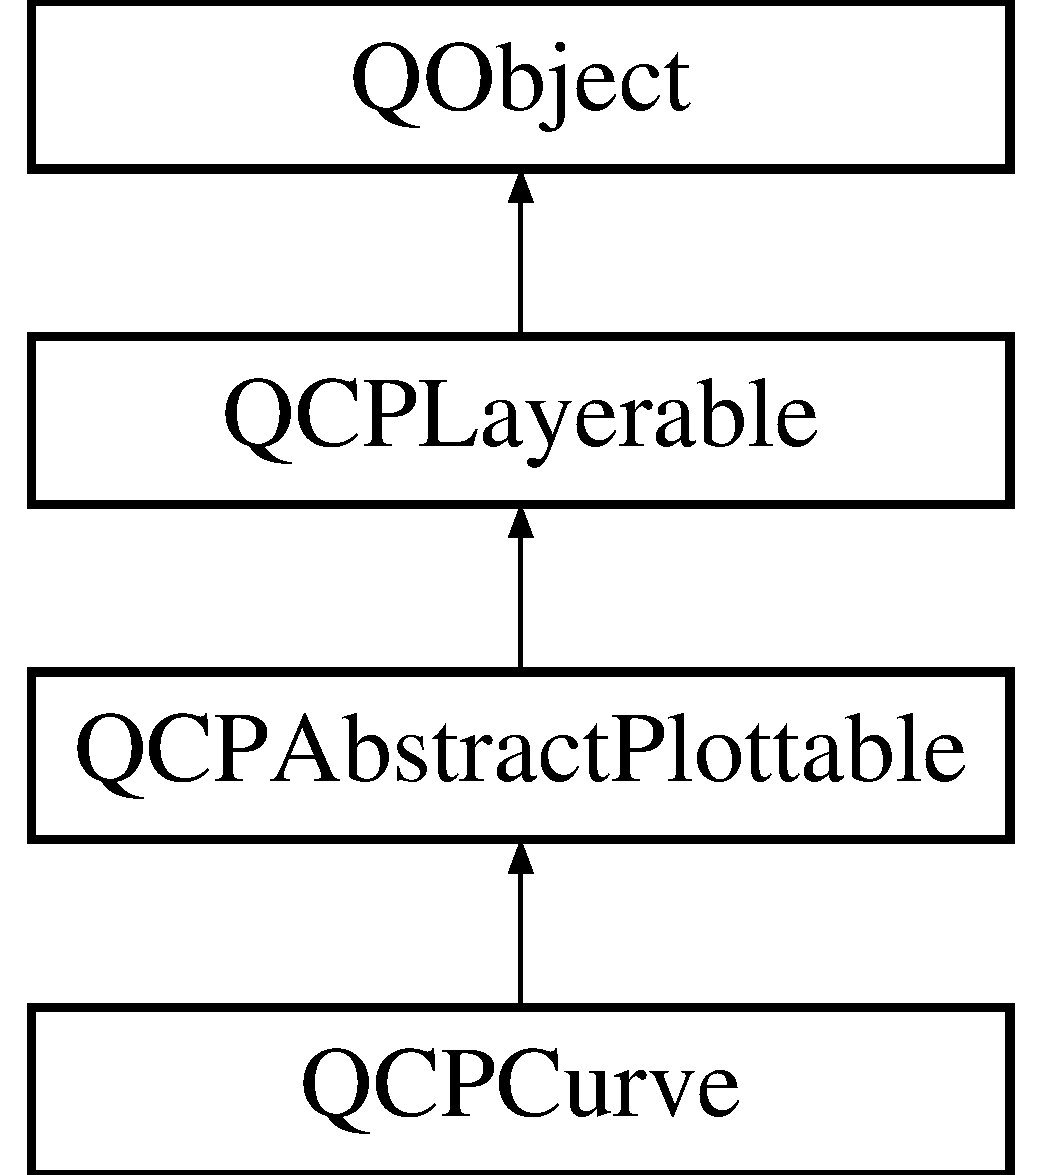
\includegraphics[height=4.000000cm]{class_q_c_p_curve}
\end{center}
\end{figure}
\subsection*{Public Types}
\begin{DoxyCompactItemize}
\item 
enum \hyperlink{class_q_c_p_curve_a2710e9f79302152cff794c6e16cc01f1}{Line\+Style} \{ \hyperlink{class_q_c_p_curve_a2710e9f79302152cff794c6e16cc01f1aec1601a191cdf0b4e761c4c66092cc48}{ls\+None}, 
\hyperlink{class_q_c_p_curve_a2710e9f79302152cff794c6e16cc01f1ade5822ce6fbf131d3df131795c2e1003}{ls\+Line}
 \}
\end{DoxyCompactItemize}
\subsection*{Public Member Functions}
\begin{DoxyCompactItemize}
\item 
\hyperlink{class_q_c_p_curve_a36de58e2652b3fa47bdf9187d421d3ce}{Q\+C\+P\+Curve} (\hyperlink{class_q_c_p_axis}{Q\+C\+P\+Axis} $\ast$key\+Axis, \hyperlink{class_q_c_p_axis}{Q\+C\+P\+Axis} $\ast$value\+Axis)
\item 
\hypertarget{class_q_c_p_curve_a667ca2594cf651e3032c624dbaa95add}{}\label{class_q_c_p_curve_a667ca2594cf651e3032c624dbaa95add} 
\hyperlink{qcustomplot_8h_a444d37ec9cb2951b3a7fe443c34d1658}{Q\+C\+P\+Curve\+Data\+Map} $\ast$ {\bfseries data} () const
\item 
\hypertarget{class_q_c_p_curve_afa6bd72a3a331a5ed45d3e0c5843b592}{}\label{class_q_c_p_curve_afa6bd72a3a331a5ed45d3e0c5843b592} 
\hyperlink{class_q_c_p_scatter_style}{Q\+C\+P\+Scatter\+Style} {\bfseries scatter\+Style} () const
\item 
\hypertarget{class_q_c_p_curve_a06e3cf3f8f1add689254b3cda66e040e}{}\label{class_q_c_p_curve_a06e3cf3f8f1add689254b3cda66e040e} 
\hyperlink{class_q_c_p_curve_a2710e9f79302152cff794c6e16cc01f1}{Line\+Style} {\bfseries line\+Style} () const
\item 
void \hyperlink{class_q_c_p_curve_a631ac886708460013b30052f49cbc9da}{set\+Data} (\hyperlink{qcustomplot_8h_a444d37ec9cb2951b3a7fe443c34d1658}{Q\+C\+P\+Curve\+Data\+Map} $\ast$data, bool copy=false)
\item 
void \hyperlink{class_q_c_p_curve_affe80e011e2ced62a88f614acd6ab8d1}{set\+Data} (const Q\+Vector$<$ double $>$ \&t, const Q\+Vector$<$ double $>$ \&key, const Q\+Vector$<$ double $>$ \&value)
\item 
void \hyperlink{class_q_c_p_curve_a963d4c45777deef15848a8f56172d066}{set\+Data} (const Q\+Vector$<$ double $>$ \&key, const Q\+Vector$<$ double $>$ \&value)
\item 
void \hyperlink{class_q_c_p_curve_a55e43b44709bf50a35500644988aa706}{set\+Scatter\+Style} (const \hyperlink{class_q_c_p_scatter_style}{Q\+C\+P\+Scatter\+Style} \&style)
\item 
void \hyperlink{class_q_c_p_curve_a4a377ec863ff81a1875c3094a6177c19}{set\+Line\+Style} (\hyperlink{class_q_c_p_curve_a2710e9f79302152cff794c6e16cc01f1}{Line\+Style} style)
\item 
void \hyperlink{class_q_c_p_curve_a4e24023c3b9ac75440c7a260172c99af}{add\+Data} (const \hyperlink{qcustomplot_8h_a444d37ec9cb2951b3a7fe443c34d1658}{Q\+C\+P\+Curve\+Data\+Map} \&data\+Map)
\item 
void \hyperlink{class_q_c_p_curve_ad304326aba096911f92452d8bfe0470e}{add\+Data} (const \hyperlink{class_q_c_p_curve_data}{Q\+C\+P\+Curve\+Data} \&data)
\item 
void \hyperlink{class_q_c_p_curve_a13398b236f6926014e404eeb5b9f415c}{add\+Data} (double t, double key, double value)
\item 
void \hyperlink{class_q_c_p_curve_ada4762e793cd5707b33f35b8a4b0f8fb}{add\+Data} (double key, double value)
\item 
void \hyperlink{class_q_c_p_curve_a27c8b3dddd4067d626397ee199626722}{add\+Data} (const Q\+Vector$<$ double $>$ \&ts, const Q\+Vector$<$ double $>$ \&keys, const Q\+Vector$<$ double $>$ \&values)
\item 
void \hyperlink{class_q_c_p_curve_af6f4284fbc2f34e676f24dce03c34fe5}{remove\+Data\+Before} (double t)
\item 
void \hyperlink{class_q_c_p_curve_a0365cb947c4e6d405ee22e00191d5f52}{remove\+Data\+After} (double t)
\item 
void \hyperlink{class_q_c_p_curve_ad45bb5479be799163028ef2b776f7221}{remove\+Data} (double fromt, double tot)
\item 
void \hyperlink{class_q_c_p_curve_a30c91acfa591ec534c49fed4c0fca39a}{remove\+Data} (double t)
\item 
virtual void \hyperlink{class_q_c_p_curve_ae0462c61dbfbac07db0736ec64110241}{clear\+Data} ()
\item 
virtual double \hyperlink{class_q_c_p_curve_a87a9fb34a2a48dcae4c1245ada235e7d}{select\+Test} (const Q\+PointF \&pos, bool only\+Selectable, Q\+Variant $\ast$details=0) const
\end{DoxyCompactItemize}
\subsection*{Protected Member Functions}
\begin{DoxyCompactItemize}
\item 
\hypertarget{class_q_c_p_curve_a2361302d2fc6ec669849bd3bca00c4b2}{}\label{class_q_c_p_curve_a2361302d2fc6ec669849bd3bca00c4b2} 
virtual void {\bfseries draw} (\hyperlink{class_q_c_p_painter}{Q\+C\+P\+Painter} $\ast$painter)
\item 
\hypertarget{class_q_c_p_curve_acccc86e9f496bb0392529f59f3a69dbc}{}\label{class_q_c_p_curve_acccc86e9f496bb0392529f59f3a69dbc} 
virtual void {\bfseries draw\+Legend\+Icon} (\hyperlink{class_q_c_p_painter}{Q\+C\+P\+Painter} $\ast$painter, const Q\+RectF \&rect) const
\item 
\hypertarget{class_q_c_p_curve_a1b24b1384d72862e8294688501ffa01d}{}\label{class_q_c_p_curve_a1b24b1384d72862e8294688501ffa01d} 
virtual \hyperlink{class_q_c_p_range}{Q\+C\+P\+Range} {\bfseries get\+Key\+Range} (bool \&found\+Range, \hyperlink{class_q_c_p_abstract_plottable_a661743478a1d3c09d28ec2711d7653d8}{Sign\+Domain} in\+Sign\+Domain=\hyperlink{class_q_c_p_abstract_plottable_a661743478a1d3c09d28ec2711d7653d8a082b98cfb91a7363a3b5cd17b0c1cd60}{sd\+Both}) const
\item 
\hypertarget{class_q_c_p_curve_a12fcfce09ffa9965b3e01555d968d378}{}\label{class_q_c_p_curve_a12fcfce09ffa9965b3e01555d968d378} 
virtual \hyperlink{class_q_c_p_range}{Q\+C\+P\+Range} {\bfseries get\+Value\+Range} (bool \&found\+Range, \hyperlink{class_q_c_p_abstract_plottable_a661743478a1d3c09d28ec2711d7653d8}{Sign\+Domain} in\+Sign\+Domain=\hyperlink{class_q_c_p_abstract_plottable_a661743478a1d3c09d28ec2711d7653d8a082b98cfb91a7363a3b5cd17b0c1cd60}{sd\+Both}) const
\item 
\hypertarget{class_q_c_p_curve_a00d17c020796ac84c84f881201c2ed10}{}\label{class_q_c_p_curve_a00d17c020796ac84c84f881201c2ed10} 
virtual void {\bfseries draw\+Scatter\+Plot} (\hyperlink{class_q_c_p_painter}{Q\+C\+P\+Painter} $\ast$painter, const Q\+Vector$<$ Q\+PointF $>$ $\ast$point\+Data) const
\item 
\hypertarget{class_q_c_p_curve_a3ca9d2c315c643f732cc85e20d18b551}{}\label{class_q_c_p_curve_a3ca9d2c315c643f732cc85e20d18b551} 
void {\bfseries get\+Curve\+Data} (Q\+Vector$<$ Q\+PointF $>$ $\ast$line\+Data) const
\item 
\hypertarget{class_q_c_p_curve_a316b216383dbff606f59c38bd72e6501}{}\label{class_q_c_p_curve_a316b216383dbff606f59c38bd72e6501} 
int {\bfseries get\+Region} (double x, double y, double rect\+Left, double rect\+Top, double rect\+Right, double rect\+Bottom) const
\item 
\hypertarget{class_q_c_p_curve_ae729c9aef90af9b7463c379cb88459f6}{}\label{class_q_c_p_curve_ae729c9aef90af9b7463c379cb88459f6} 
Q\+PointF {\bfseries get\+Optimized\+Point} (int prev\+Region, double prev\+Key, double prev\+Value, double key, double value, double rect\+Left, double rect\+Top, double rect\+Right, double rect\+Bottom) const
\item 
\hypertarget{class_q_c_p_curve_a2f1455455d71de9ef9190c50a90f0abc}{}\label{class_q_c_p_curve_a2f1455455d71de9ef9190c50a90f0abc} 
Q\+Vector$<$ Q\+PointF $>$ {\bfseries get\+Optimized\+Corner\+Points} (int prev\+Region, int current\+Region, double prev\+Key, double prev\+Value, double key, double value, double rect\+Left, double rect\+Top, double rect\+Right, double rect\+Bottom) const
\item 
\hypertarget{class_q_c_p_curve_af5df2560b30333fe662ec676bd355415}{}\label{class_q_c_p_curve_af5df2560b30333fe662ec676bd355415} 
bool {\bfseries may\+Traverse} (int prev\+Region, int current\+Region) const
\item 
\hypertarget{class_q_c_p_curve_a82a78dffde71e7b9c40217fa7e381057}{}\label{class_q_c_p_curve_a82a78dffde71e7b9c40217fa7e381057} 
bool {\bfseries get\+Traverse} (double prev\+Key, double prev\+Value, double key, double value, double rect\+Left, double rect\+Top, double rect\+Right, double rect\+Bottom, Q\+PointF \&crossA, Q\+PointF \&crossB) const
\item 
\hypertarget{class_q_c_p_curve_a592d6e3dbd42cb8cea35eda889ece1b1}{}\label{class_q_c_p_curve_a592d6e3dbd42cb8cea35eda889ece1b1} 
void {\bfseries get\+Traverse\+Corner\+Points} (int prev\+Region, int current\+Region, double rect\+Left, double rect\+Top, double rect\+Right, double rect\+Bottom, Q\+Vector$<$ Q\+PointF $>$ \&before\+Traverse, Q\+Vector$<$ Q\+PointF $>$ \&after\+Traverse) const
\item 
\hypertarget{class_q_c_p_curve_adc3ab8051946f9097cdf7c0707ef1a25}{}\label{class_q_c_p_curve_adc3ab8051946f9097cdf7c0707ef1a25} 
double {\bfseries point\+Distance} (const Q\+PointF \&pixel\+Point) const
\end{DoxyCompactItemize}
\subsection*{Protected Attributes}
\begin{DoxyCompactItemize}
\item 
\hypertarget{class_q_c_p_curve_a88d533e455bca96004b049e99168731b}{}\label{class_q_c_p_curve_a88d533e455bca96004b049e99168731b} 
\hyperlink{qcustomplot_8h_a444d37ec9cb2951b3a7fe443c34d1658}{Q\+C\+P\+Curve\+Data\+Map} $\ast$ {\bfseries m\+Data}
\item 
\hypertarget{class_q_c_p_curve_a08f803b4a30b01bbd7a1eab15d0f864f}{}\label{class_q_c_p_curve_a08f803b4a30b01bbd7a1eab15d0f864f} 
\hyperlink{class_q_c_p_scatter_style}{Q\+C\+P\+Scatter\+Style} {\bfseries m\+Scatter\+Style}
\item 
\hypertarget{class_q_c_p_curve_ae1f35ae2b15aee8e15bcdfec5be95156}{}\label{class_q_c_p_curve_ae1f35ae2b15aee8e15bcdfec5be95156} 
\hyperlink{class_q_c_p_curve_a2710e9f79302152cff794c6e16cc01f1}{Line\+Style} {\bfseries m\+Line\+Style}
\end{DoxyCompactItemize}
\subsection*{Friends}
\begin{DoxyCompactItemize}
\item 
\hypertarget{class_q_c_p_curve_a1cdf9df76adcfae45261690aa0ca2198}{}\label{class_q_c_p_curve_a1cdf9df76adcfae45261690aa0ca2198} 
class {\bfseries Q\+Custom\+Plot}
\item 
\hypertarget{class_q_c_p_curve_a8429035e7adfbd7f05805a6530ad5e3b}{}\label{class_q_c_p_curve_a8429035e7adfbd7f05805a6530ad5e3b} 
class {\bfseries Q\+C\+P\+Legend}
\end{DoxyCompactItemize}
\subsection*{Additional Inherited Members}


\subsection{Detailed Description}
A plottable representing a parametric curve in a plot. 



Unlike \hyperlink{class_q_c_p_graph}{Q\+C\+P\+Graph}, plottables of this type may have multiple points with the same key coordinate, so their visual representation can have {\itshape loops}. This is realized by introducing a third coordinate {\itshape t}, which defines the order of the points described by the other two coordinates {\itshape x} and {\itshape y}.

To plot data, assign it with the \hyperlink{class_q_c_p_curve_a631ac886708460013b30052f49cbc9da}{set\+Data} or \hyperlink{class_q_c_p_curve_a4e24023c3b9ac75440c7a260172c99af}{add\+Data} functions.

Gaps in the curve can be created by adding data points with NaN as key and value ({\ttfamily q\+Q\+Na\+N()} or {\ttfamily std\+::numeric\+\_\+limits$<$double$>$\+::quiet\+\_\+\+Na\+N()}) in between the two data points that shall be separated.\hypertarget{class_q_c_p_statistical_box_appearance}{}\subsection{Changing the appearance}\label{class_q_c_p_statistical_box_appearance}
The appearance of the curve is determined by the pen and the brush (\hyperlink{class_q_c_p_abstract_plottable_ab74b09ae4c0e7e13142fe4b5bf46cac7}{set\+Pen}, \hyperlink{class_q_c_p_abstract_plottable_a7a4b92144dca6453a1f0f210e27edc74}{set\+Brush}). \hypertarget{class_q_c_p_statistical_box_usage}{}\subsection{Usage}\label{class_q_c_p_statistical_box_usage}
Like all data representing objects in \hyperlink{class_q_custom_plot}{Q\+Custom\+Plot}, the \hyperlink{class_q_c_p_curve}{Q\+C\+P\+Curve} is a plottable (\hyperlink{class_q_c_p_abstract_plottable}{Q\+C\+P\+Abstract\+Plottable}). So the plottable-\/interface of \hyperlink{class_q_custom_plot}{Q\+Custom\+Plot} applies (\hyperlink{class_q_custom_plot_a32de81ff53e263e785b83b52ecd99d6f}{Q\+Custom\+Plot\+::plottable}, \hyperlink{class_q_custom_plot_ab7ad9174f701f9c6f64e378df77927a6}{Q\+Custom\+Plot\+::add\+Plottable}, \hyperlink{class_q_custom_plot_af3dafd56884208474f311d6226513ab2}{Q\+Custom\+Plot\+::remove\+Plottable}, etc.)

Usually, you first create an instance and add it to the custom\+Plot\+: 
\begin{DoxyCodeInclude}
\end{DoxyCodeInclude}
and then modify the properties of the newly created plottable, e.\+g.\+: 
\begin{DoxyCodeInclude}
\end{DoxyCodeInclude}


\subsection{Member Enumeration Documentation}
\hypertarget{class_q_c_p_curve_a2710e9f79302152cff794c6e16cc01f1}{}\label{class_q_c_p_curve_a2710e9f79302152cff794c6e16cc01f1} 
\index{Q\+C\+P\+Curve@{Q\+C\+P\+Curve}!Line\+Style@{Line\+Style}}
\index{Line\+Style@{Line\+Style}!Q\+C\+P\+Curve@{Q\+C\+P\+Curve}}
\subsubsection{\texorpdfstring{Line\+Style}{LineStyle}}
{\footnotesize\ttfamily enum \hyperlink{class_q_c_p_curve_a2710e9f79302152cff794c6e16cc01f1}{Q\+C\+P\+Curve\+::\+Line\+Style}}

Defines how the curve\textquotesingle{}s line is represented visually in the plot. The line is drawn with the current pen of the curve (\hyperlink{class_q_c_p_abstract_plottable_ab74b09ae4c0e7e13142fe4b5bf46cac7}{set\+Pen}). \begin{DoxySeeAlso}{See also}
\hyperlink{class_q_c_p_curve_a4a377ec863ff81a1875c3094a6177c19}{set\+Line\+Style} 
\end{DoxySeeAlso}
\begin{DoxyEnumFields}{Enumerator}
\raisebox{\heightof{T}}[0pt][0pt]{\index{ls\+None@{ls\+None}!Q\+C\+P\+Curve@{Q\+C\+P\+Curve}}\index{Q\+C\+P\+Curve@{Q\+C\+P\+Curve}!ls\+None@{ls\+None}}}\hypertarget{class_q_c_p_curve_a2710e9f79302152cff794c6e16cc01f1aec1601a191cdf0b4e761c4c66092cc48}{}\label{class_q_c_p_curve_a2710e9f79302152cff794c6e16cc01f1aec1601a191cdf0b4e761c4c66092cc48} 
ls\+None&No line is drawn between data points (e.\+g. only scatters) \\
\hline

\raisebox{\heightof{T}}[0pt][0pt]{\index{ls\+Line@{ls\+Line}!Q\+C\+P\+Curve@{Q\+C\+P\+Curve}}\index{Q\+C\+P\+Curve@{Q\+C\+P\+Curve}!ls\+Line@{ls\+Line}}}\hypertarget{class_q_c_p_curve_a2710e9f79302152cff794c6e16cc01f1ade5822ce6fbf131d3df131795c2e1003}{}\label{class_q_c_p_curve_a2710e9f79302152cff794c6e16cc01f1ade5822ce6fbf131d3df131795c2e1003} 
ls\+Line&Data points are connected with a straight line. \\
\hline

\end{DoxyEnumFields}


\subsection{Constructor \& Destructor Documentation}
\hypertarget{class_q_c_p_curve_a36de58e2652b3fa47bdf9187d421d3ce}{}\label{class_q_c_p_curve_a36de58e2652b3fa47bdf9187d421d3ce} 
\index{Q\+C\+P\+Curve@{Q\+C\+P\+Curve}!Q\+C\+P\+Curve@{Q\+C\+P\+Curve}}
\index{Q\+C\+P\+Curve@{Q\+C\+P\+Curve}!Q\+C\+P\+Curve@{Q\+C\+P\+Curve}}
\subsubsection{\texorpdfstring{Q\+C\+P\+Curve()}{QCPCurve()}}
{\footnotesize\ttfamily Q\+C\+P\+Curve\+::\+Q\+C\+P\+Curve (\begin{DoxyParamCaption}\item[{\hyperlink{class_q_c_p_axis}{Q\+C\+P\+Axis} $\ast$}]{key\+Axis,  }\item[{\hyperlink{class_q_c_p_axis}{Q\+C\+P\+Axis} $\ast$}]{value\+Axis }\end{DoxyParamCaption})\hspace{0.3cm}{\ttfamily [explicit]}}

Constructs a curve which uses {\itshape key\+Axis} as its key axis (\char`\"{}x\char`\"{}) and {\itshape value\+Axis} as its value axis (\char`\"{}y\char`\"{}). {\itshape key\+Axis} and {\itshape value\+Axis} must reside in the same \hyperlink{class_q_custom_plot}{Q\+Custom\+Plot} instance and not have the same orientation. If either of these restrictions is violated, a corresponding message is printed to the debug output (q\+Debug), the construction is not aborted, though.

The constructed \hyperlink{class_q_c_p_curve}{Q\+C\+P\+Curve} can be added to the plot with \hyperlink{class_q_custom_plot_ab7ad9174f701f9c6f64e378df77927a6}{Q\+Custom\+Plot\+::add\+Plottable}, \hyperlink{class_q_custom_plot}{Q\+Custom\+Plot} then takes ownership of the graph. 

\subsection{Member Function Documentation}
\hypertarget{class_q_c_p_curve_a4e24023c3b9ac75440c7a260172c99af}{}\label{class_q_c_p_curve_a4e24023c3b9ac75440c7a260172c99af} 
\index{Q\+C\+P\+Curve@{Q\+C\+P\+Curve}!add\+Data@{add\+Data}}
\index{add\+Data@{add\+Data}!Q\+C\+P\+Curve@{Q\+C\+P\+Curve}}
\subsubsection{\texorpdfstring{add\+Data()}{addData()}\hspace{0.1cm}{\footnotesize\ttfamily [1/5]}}
{\footnotesize\ttfamily void Q\+C\+P\+Curve\+::add\+Data (\begin{DoxyParamCaption}\item[{const \hyperlink{qcustomplot_8h_a444d37ec9cb2951b3a7fe443c34d1658}{Q\+C\+P\+Curve\+Data\+Map} \&}]{data\+Map }\end{DoxyParamCaption})}

Adds the provided data points in {\itshape data\+Map} to the current data. \begin{DoxySeeAlso}{See also}
\hyperlink{class_q_c_p_curve_ad45bb5479be799163028ef2b776f7221}{remove\+Data} 
\end{DoxySeeAlso}
\hypertarget{class_q_c_p_curve_ad304326aba096911f92452d8bfe0470e}{}\label{class_q_c_p_curve_ad304326aba096911f92452d8bfe0470e} 
\index{Q\+C\+P\+Curve@{Q\+C\+P\+Curve}!add\+Data@{add\+Data}}
\index{add\+Data@{add\+Data}!Q\+C\+P\+Curve@{Q\+C\+P\+Curve}}
\subsubsection{\texorpdfstring{add\+Data()}{addData()}\hspace{0.1cm}{\footnotesize\ttfamily [2/5]}}
{\footnotesize\ttfamily void Q\+C\+P\+Curve\+::add\+Data (\begin{DoxyParamCaption}\item[{const \hyperlink{class_q_c_p_curve_data}{Q\+C\+P\+Curve\+Data} \&}]{data }\end{DoxyParamCaption})}

This is an overloaded member function, provided for convenience. It differs from the above function only in what argument(s) it accepts. Adds the provided single data point in {\itshape data} to the current data. \begin{DoxySeeAlso}{See also}
\hyperlink{class_q_c_p_curve_ad45bb5479be799163028ef2b776f7221}{remove\+Data} 
\end{DoxySeeAlso}
\hypertarget{class_q_c_p_curve_a13398b236f6926014e404eeb5b9f415c}{}\label{class_q_c_p_curve_a13398b236f6926014e404eeb5b9f415c} 
\index{Q\+C\+P\+Curve@{Q\+C\+P\+Curve}!add\+Data@{add\+Data}}
\index{add\+Data@{add\+Data}!Q\+C\+P\+Curve@{Q\+C\+P\+Curve}}
\subsubsection{\texorpdfstring{add\+Data()}{addData()}\hspace{0.1cm}{\footnotesize\ttfamily [3/5]}}
{\footnotesize\ttfamily void Q\+C\+P\+Curve\+::add\+Data (\begin{DoxyParamCaption}\item[{double}]{t,  }\item[{double}]{key,  }\item[{double}]{value }\end{DoxyParamCaption})}

This is an overloaded member function, provided for convenience. It differs from the above function only in what argument(s) it accepts. Adds the provided single data point as {\itshape t}, {\itshape key} and {\itshape value} tuple to the current data \begin{DoxySeeAlso}{See also}
\hyperlink{class_q_c_p_curve_ad45bb5479be799163028ef2b776f7221}{remove\+Data} 
\end{DoxySeeAlso}
\hypertarget{class_q_c_p_curve_ada4762e793cd5707b33f35b8a4b0f8fb}{}\label{class_q_c_p_curve_ada4762e793cd5707b33f35b8a4b0f8fb} 
\index{Q\+C\+P\+Curve@{Q\+C\+P\+Curve}!add\+Data@{add\+Data}}
\index{add\+Data@{add\+Data}!Q\+C\+P\+Curve@{Q\+C\+P\+Curve}}
\subsubsection{\texorpdfstring{add\+Data()}{addData()}\hspace{0.1cm}{\footnotesize\ttfamily [4/5]}}
{\footnotesize\ttfamily void Q\+C\+P\+Curve\+::add\+Data (\begin{DoxyParamCaption}\item[{double}]{key,  }\item[{double}]{value }\end{DoxyParamCaption})}

This is an overloaded member function, provided for convenience. It differs from the above function only in what argument(s) it accepts.

Adds the provided single data point as {\itshape key} and {\itshape value} pair to the current data The t parameter of the data point is set to the t of the last data point plus 1. If there is no last data point, t will be set to 0.

\begin{DoxySeeAlso}{See also}
\hyperlink{class_q_c_p_curve_ad45bb5479be799163028ef2b776f7221}{remove\+Data} 
\end{DoxySeeAlso}
\hypertarget{class_q_c_p_curve_a27c8b3dddd4067d626397ee199626722}{}\label{class_q_c_p_curve_a27c8b3dddd4067d626397ee199626722} 
\index{Q\+C\+P\+Curve@{Q\+C\+P\+Curve}!add\+Data@{add\+Data}}
\index{add\+Data@{add\+Data}!Q\+C\+P\+Curve@{Q\+C\+P\+Curve}}
\subsubsection{\texorpdfstring{add\+Data()}{addData()}\hspace{0.1cm}{\footnotesize\ttfamily [5/5]}}
{\footnotesize\ttfamily void Q\+C\+P\+Curve\+::add\+Data (\begin{DoxyParamCaption}\item[{const Q\+Vector$<$ double $>$ \&}]{ts,  }\item[{const Q\+Vector$<$ double $>$ \&}]{keys,  }\item[{const Q\+Vector$<$ double $>$ \&}]{values }\end{DoxyParamCaption})}

This is an overloaded member function, provided for convenience. It differs from the above function only in what argument(s) it accepts. Adds the provided data points as {\itshape t}, {\itshape key} and {\itshape value} tuples to the current data. \begin{DoxySeeAlso}{See also}
\hyperlink{class_q_c_p_curve_ad45bb5479be799163028ef2b776f7221}{remove\+Data} 
\end{DoxySeeAlso}
\hypertarget{class_q_c_p_curve_ae0462c61dbfbac07db0736ec64110241}{}\label{class_q_c_p_curve_ae0462c61dbfbac07db0736ec64110241} 
\index{Q\+C\+P\+Curve@{Q\+C\+P\+Curve}!clear\+Data@{clear\+Data}}
\index{clear\+Data@{clear\+Data}!Q\+C\+P\+Curve@{Q\+C\+P\+Curve}}
\subsubsection{\texorpdfstring{clear\+Data()}{clearData()}}
{\footnotesize\ttfamily void Q\+C\+P\+Curve\+::clear\+Data (\begin{DoxyParamCaption}{ }\end{DoxyParamCaption})\hspace{0.3cm}{\ttfamily [virtual]}}

Removes all data points. \begin{DoxySeeAlso}{See also}
\hyperlink{class_q_c_p_curve_ad45bb5479be799163028ef2b776f7221}{remove\+Data}, \hyperlink{class_q_c_p_curve_a0365cb947c4e6d405ee22e00191d5f52}{remove\+Data\+After}, \hyperlink{class_q_c_p_curve_af6f4284fbc2f34e676f24dce03c34fe5}{remove\+Data\+Before} 
\end{DoxySeeAlso}


Implements \hyperlink{class_q_c_p_abstract_plottable_a86e5b8fd4b6ff4f4084e7ea4c573fc53}{Q\+C\+P\+Abstract\+Plottable}.

\hypertarget{class_q_c_p_curve_ad45bb5479be799163028ef2b776f7221}{}\label{class_q_c_p_curve_ad45bb5479be799163028ef2b776f7221} 
\index{Q\+C\+P\+Curve@{Q\+C\+P\+Curve}!remove\+Data@{remove\+Data}}
\index{remove\+Data@{remove\+Data}!Q\+C\+P\+Curve@{Q\+C\+P\+Curve}}
\subsubsection{\texorpdfstring{remove\+Data()}{removeData()}\hspace{0.1cm}{\footnotesize\ttfamily [1/2]}}
{\footnotesize\ttfamily void Q\+C\+P\+Curve\+::remove\+Data (\begin{DoxyParamCaption}\item[{double}]{fromt,  }\item[{double}]{tot }\end{DoxyParamCaption})}

Removes all data points with curve parameter t between {\itshape fromt} and {\itshape tot}. if {\itshape fromt} is greater or equal to {\itshape tot}, the function does nothing. To remove a single data point with known t, use \hyperlink{class_q_c_p_curve_a30c91acfa591ec534c49fed4c0fca39a}{remove\+Data(double t)}.

\begin{DoxySeeAlso}{See also}
\hyperlink{class_q_c_p_curve_a4e24023c3b9ac75440c7a260172c99af}{add\+Data}, \hyperlink{class_q_c_p_curve_ae0462c61dbfbac07db0736ec64110241}{clear\+Data} 
\end{DoxySeeAlso}
\hypertarget{class_q_c_p_curve_a30c91acfa591ec534c49fed4c0fca39a}{}\label{class_q_c_p_curve_a30c91acfa591ec534c49fed4c0fca39a} 
\index{Q\+C\+P\+Curve@{Q\+C\+P\+Curve}!remove\+Data@{remove\+Data}}
\index{remove\+Data@{remove\+Data}!Q\+C\+P\+Curve@{Q\+C\+P\+Curve}}
\subsubsection{\texorpdfstring{remove\+Data()}{removeData()}\hspace{0.1cm}{\footnotesize\ttfamily [2/2]}}
{\footnotesize\ttfamily void Q\+C\+P\+Curve\+::remove\+Data (\begin{DoxyParamCaption}\item[{double}]{t }\end{DoxyParamCaption})}

This is an overloaded member function, provided for convenience. It differs from the above function only in what argument(s) it accepts.

Removes a single data point at curve parameter {\itshape t}. If the position is not known with absolute precision, consider using \hyperlink{class_q_c_p_curve_ad45bb5479be799163028ef2b776f7221}{remove\+Data(double fromt, double tot)} with a small fuzziness interval around the suspected position, depeding on the precision with which the curve parameter is known.

\begin{DoxySeeAlso}{See also}
\hyperlink{class_q_c_p_curve_a4e24023c3b9ac75440c7a260172c99af}{add\+Data}, \hyperlink{class_q_c_p_curve_ae0462c61dbfbac07db0736ec64110241}{clear\+Data} 
\end{DoxySeeAlso}
\hypertarget{class_q_c_p_curve_a0365cb947c4e6d405ee22e00191d5f52}{}\label{class_q_c_p_curve_a0365cb947c4e6d405ee22e00191d5f52} 
\index{Q\+C\+P\+Curve@{Q\+C\+P\+Curve}!remove\+Data\+After@{remove\+Data\+After}}
\index{remove\+Data\+After@{remove\+Data\+After}!Q\+C\+P\+Curve@{Q\+C\+P\+Curve}}
\subsubsection{\texorpdfstring{remove\+Data\+After()}{removeDataAfter()}}
{\footnotesize\ttfamily void Q\+C\+P\+Curve\+::remove\+Data\+After (\begin{DoxyParamCaption}\item[{double}]{t }\end{DoxyParamCaption})}

Removes all data points with curve parameter t greater than {\itshape t}. \begin{DoxySeeAlso}{See also}
\hyperlink{class_q_c_p_curve_a4e24023c3b9ac75440c7a260172c99af}{add\+Data}, \hyperlink{class_q_c_p_curve_ae0462c61dbfbac07db0736ec64110241}{clear\+Data} 
\end{DoxySeeAlso}
\hypertarget{class_q_c_p_curve_af6f4284fbc2f34e676f24dce03c34fe5}{}\label{class_q_c_p_curve_af6f4284fbc2f34e676f24dce03c34fe5} 
\index{Q\+C\+P\+Curve@{Q\+C\+P\+Curve}!remove\+Data\+Before@{remove\+Data\+Before}}
\index{remove\+Data\+Before@{remove\+Data\+Before}!Q\+C\+P\+Curve@{Q\+C\+P\+Curve}}
\subsubsection{\texorpdfstring{remove\+Data\+Before()}{removeDataBefore()}}
{\footnotesize\ttfamily void Q\+C\+P\+Curve\+::remove\+Data\+Before (\begin{DoxyParamCaption}\item[{double}]{t }\end{DoxyParamCaption})}

Removes all data points with curve parameter t smaller than {\itshape t}. \begin{DoxySeeAlso}{See also}
\hyperlink{class_q_c_p_curve_a4e24023c3b9ac75440c7a260172c99af}{add\+Data}, \hyperlink{class_q_c_p_curve_ae0462c61dbfbac07db0736ec64110241}{clear\+Data} 
\end{DoxySeeAlso}
\hypertarget{class_q_c_p_curve_a87a9fb34a2a48dcae4c1245ada235e7d}{}\label{class_q_c_p_curve_a87a9fb34a2a48dcae4c1245ada235e7d} 
\index{Q\+C\+P\+Curve@{Q\+C\+P\+Curve}!select\+Test@{select\+Test}}
\index{select\+Test@{select\+Test}!Q\+C\+P\+Curve@{Q\+C\+P\+Curve}}
\subsubsection{\texorpdfstring{select\+Test()}{selectTest()}}
{\footnotesize\ttfamily double Q\+C\+P\+Curve\+::select\+Test (\begin{DoxyParamCaption}\item[{const Q\+PointF \&}]{pos,  }\item[{bool}]{only\+Selectable,  }\item[{Q\+Variant $\ast$}]{details = {\ttfamily 0} }\end{DoxyParamCaption}) const\hspace{0.3cm}{\ttfamily [virtual]}}

This function is used to decide whether a click hits a layerable object or not.

{\itshape pos} is a point in pixel coordinates on the \hyperlink{class_q_custom_plot}{Q\+Custom\+Plot} surface. This function returns the shortest pixel distance of this point to the object. If the object is either invisible or the distance couldn\textquotesingle{}t be determined, -\/1.\+0 is returned. Further, if {\itshape only\+Selectable} is true and the object is not selectable, -\/1.\+0 is returned, too.

If the object is represented not by single lines but by an area like a \hyperlink{class_q_c_p_item_text}{Q\+C\+P\+Item\+Text} or the bars of a \hyperlink{class_q_c_p_bars}{Q\+C\+P\+Bars} plottable, a click inside the area should also be considered a hit. In these cases this function thus returns a constant value greater zero but still below the parent plot\textquotesingle{}s selection tolerance. (typically the selection\+Tolerance multiplied by 0.\+99).

Providing a constant value for area objects allows selecting line objects even when they are obscured by such area objects, by clicking close to the lines (i.\+e. closer than 0.\+99$\ast$selection\+Tolerance).

The actual setting of the selection state is not done by this function. This is handled by the parent \hyperlink{class_q_custom_plot}{Q\+Custom\+Plot} when the mouse\+Release\+Event occurs, and the finally selected object is notified via the select\+Event/deselect\+Event methods.

{\itshape details} is an optional output parameter. Every layerable subclass may place any information in {\itshape details}. This information will be passed to select\+Event when the parent \hyperlink{class_q_custom_plot}{Q\+Custom\+Plot} decides on the basis of this select\+Test call, that the object was successfully selected. The subsequent call to select\+Event will carry the {\itshape details}. This is useful for multi-\/part objects (like \hyperlink{class_q_c_p_axis}{Q\+C\+P\+Axis}). This way, a possibly complex calculation to decide which part was clicked is only done once in \hyperlink{class_q_c_p_curve_a87a9fb34a2a48dcae4c1245ada235e7d}{select\+Test}. The result (i.\+e. the actually clicked part) can then be placed in {\itshape details}. So in the subsequent select\+Event, the decision which part was selected doesn\textquotesingle{}t have to be done a second time for a single selection operation.

You may pass 0 as {\itshape details} to indicate that you are not interested in those selection details.

\begin{DoxySeeAlso}{See also}
select\+Event, deselect\+Event, \hyperlink{class_q_custom_plot_a5ee1e2f6ae27419deca53e75907c27e5}{Q\+Custom\+Plot\+::set\+Interactions} 
\end{DoxySeeAlso}


Implements \hyperlink{class_q_c_p_abstract_plottable_a38efe9641d972992a3d44204bc80ec1d}{Q\+C\+P\+Abstract\+Plottable}.

\hypertarget{class_q_c_p_curve_a631ac886708460013b30052f49cbc9da}{}\label{class_q_c_p_curve_a631ac886708460013b30052f49cbc9da} 
\index{Q\+C\+P\+Curve@{Q\+C\+P\+Curve}!set\+Data@{set\+Data}}
\index{set\+Data@{set\+Data}!Q\+C\+P\+Curve@{Q\+C\+P\+Curve}}
\subsubsection{\texorpdfstring{set\+Data()}{setData()}\hspace{0.1cm}{\footnotesize\ttfamily [1/3]}}
{\footnotesize\ttfamily void Q\+C\+P\+Curve\+::set\+Data (\begin{DoxyParamCaption}\item[{\hyperlink{qcustomplot_8h_a444d37ec9cb2951b3a7fe443c34d1658}{Q\+C\+P\+Curve\+Data\+Map} $\ast$}]{data,  }\item[{bool}]{copy = {\ttfamily false} }\end{DoxyParamCaption})}

Replaces the current data with the provided {\itshape data}.

If {\itshape copy} is set to true, data points in {\itshape data} will only be copied. if false, the plottable takes ownership of the passed data and replaces the internal data pointer with it. This is significantly faster than copying for large datasets. \hypertarget{class_q_c_p_curve_affe80e011e2ced62a88f614acd6ab8d1}{}\label{class_q_c_p_curve_affe80e011e2ced62a88f614acd6ab8d1} 
\index{Q\+C\+P\+Curve@{Q\+C\+P\+Curve}!set\+Data@{set\+Data}}
\index{set\+Data@{set\+Data}!Q\+C\+P\+Curve@{Q\+C\+P\+Curve}}
\subsubsection{\texorpdfstring{set\+Data()}{setData()}\hspace{0.1cm}{\footnotesize\ttfamily [2/3]}}
{\footnotesize\ttfamily void Q\+C\+P\+Curve\+::set\+Data (\begin{DoxyParamCaption}\item[{const Q\+Vector$<$ double $>$ \&}]{t,  }\item[{const Q\+Vector$<$ double $>$ \&}]{key,  }\item[{const Q\+Vector$<$ double $>$ \&}]{value }\end{DoxyParamCaption})}

This is an overloaded member function, provided for convenience. It differs from the above function only in what argument(s) it accepts.

Replaces the current data with the provided points in {\itshape t}, {\itshape key} and {\itshape value} tuples. The provided vectors should have equal length. Else, the number of added points will be the size of the smallest vector. \hypertarget{class_q_c_p_curve_a963d4c45777deef15848a8f56172d066}{}\label{class_q_c_p_curve_a963d4c45777deef15848a8f56172d066} 
\index{Q\+C\+P\+Curve@{Q\+C\+P\+Curve}!set\+Data@{set\+Data}}
\index{set\+Data@{set\+Data}!Q\+C\+P\+Curve@{Q\+C\+P\+Curve}}
\subsubsection{\texorpdfstring{set\+Data()}{setData()}\hspace{0.1cm}{\footnotesize\ttfamily [3/3]}}
{\footnotesize\ttfamily void Q\+C\+P\+Curve\+::set\+Data (\begin{DoxyParamCaption}\item[{const Q\+Vector$<$ double $>$ \&}]{key,  }\item[{const Q\+Vector$<$ double $>$ \&}]{value }\end{DoxyParamCaption})}

This is an overloaded member function, provided for convenience. It differs from the above function only in what argument(s) it accepts.

Replaces the current data with the provided {\itshape key} and {\itshape value} pairs. The t parameter of each data point will be set to the integer index of the respective key/value pair. \hypertarget{class_q_c_p_curve_a4a377ec863ff81a1875c3094a6177c19}{}\label{class_q_c_p_curve_a4a377ec863ff81a1875c3094a6177c19} 
\index{Q\+C\+P\+Curve@{Q\+C\+P\+Curve}!set\+Line\+Style@{set\+Line\+Style}}
\index{set\+Line\+Style@{set\+Line\+Style}!Q\+C\+P\+Curve@{Q\+C\+P\+Curve}}
\subsubsection{\texorpdfstring{set\+Line\+Style()}{setLineStyle()}}
{\footnotesize\ttfamily void Q\+C\+P\+Curve\+::set\+Line\+Style (\begin{DoxyParamCaption}\item[{\hyperlink{class_q_c_p_curve_a2710e9f79302152cff794c6e16cc01f1}{Q\+C\+P\+Curve\+::\+Line\+Style}}]{style }\end{DoxyParamCaption})}

Sets how the single data points are connected in the plot or how they are represented visually apart from the scatter symbol. For scatter-\/only plots, set {\itshape style} to \hyperlink{class_q_c_p_curve_a2710e9f79302152cff794c6e16cc01f1aec1601a191cdf0b4e761c4c66092cc48}{ls\+None} and \hyperlink{class_q_c_p_curve_a55e43b44709bf50a35500644988aa706}{set\+Scatter\+Style} to the desired scatter style.

\begin{DoxySeeAlso}{See also}
\hyperlink{class_q_c_p_curve_a55e43b44709bf50a35500644988aa706}{set\+Scatter\+Style} 
\end{DoxySeeAlso}
\hypertarget{class_q_c_p_curve_a55e43b44709bf50a35500644988aa706}{}\label{class_q_c_p_curve_a55e43b44709bf50a35500644988aa706} 
\index{Q\+C\+P\+Curve@{Q\+C\+P\+Curve}!set\+Scatter\+Style@{set\+Scatter\+Style}}
\index{set\+Scatter\+Style@{set\+Scatter\+Style}!Q\+C\+P\+Curve@{Q\+C\+P\+Curve}}
\subsubsection{\texorpdfstring{set\+Scatter\+Style()}{setScatterStyle()}}
{\footnotesize\ttfamily void Q\+C\+P\+Curve\+::set\+Scatter\+Style (\begin{DoxyParamCaption}\item[{const \hyperlink{class_q_c_p_scatter_style}{Q\+C\+P\+Scatter\+Style} \&}]{style }\end{DoxyParamCaption})}

Sets the visual appearance of single data points in the plot. If set to \hyperlink{class_q_c_p_scatter_style_adb31525af6b680e6f1b7472e43859349abd144c291ca274f77053ec68cab6c022}{Q\+C\+P\+Scatter\+Style\+::ss\+None}, no scatter points are drawn (e.\+g. for line-\/only plots with appropriate line style).

\begin{DoxySeeAlso}{See also}
\hyperlink{class_q_c_p_scatter_style}{Q\+C\+P\+Scatter\+Style}, \hyperlink{class_q_c_p_curve_a4a377ec863ff81a1875c3094a6177c19}{set\+Line\+Style} 
\end{DoxySeeAlso}


The documentation for this class was generated from the following files\+:\begin{DoxyCompactItemize}
\item 
F\+E\+S\+S-\/\+G\+U\+I/\hyperlink{qcustomplot_8h}{qcustomplot.\+h}\item 
F\+E\+S\+S-\/\+G\+U\+I/\hyperlink{qcustomplot_8cpp}{qcustomplot.\+cpp}\end{DoxyCompactItemize}

\hypertarget{class_q_c_p_curve_data}{}\section{Q\+C\+P\+Curve\+Data Class Reference}
\label{class_q_c_p_curve_data}\index{Q\+C\+P\+Curve\+Data@{Q\+C\+P\+Curve\+Data}}


Holds the data of one single data point for \hyperlink{class_q_c_p_curve}{Q\+C\+P\+Curve}.  


\subsection*{Public Member Functions}
\begin{DoxyCompactItemize}
\item 
\hyperlink{class_q_c_p_curve_data_a48252779b5198a509d99c69ae223fbf8}{Q\+C\+P\+Curve\+Data} ()
\item 
\hyperlink{class_q_c_p_curve_data_a3586be0cc6f8db15bcdd0c0d03b0c173}{Q\+C\+P\+Curve\+Data} (double t, double key, double value)
\end{DoxyCompactItemize}
\subsection*{Public Attributes}
\begin{DoxyCompactItemize}
\item 
\hypertarget{class_q_c_p_curve_data_aecc395525be28e9178a088793beb3ff3}{}\label{class_q_c_p_curve_data_aecc395525be28e9178a088793beb3ff3} 
double {\bfseries t}
\item 
\hypertarget{class_q_c_p_curve_data_a8a4ec5f2b9a396149fd842e309701bd4}{}\label{class_q_c_p_curve_data_a8a4ec5f2b9a396149fd842e309701bd4} 
double {\bfseries key}
\item 
\hypertarget{class_q_c_p_curve_data_a72b39b8e1dbf7b45382ebd48419b6828}{}\label{class_q_c_p_curve_data_a72b39b8e1dbf7b45382ebd48419b6828} 
double {\bfseries value}
\end{DoxyCompactItemize}


\subsection{Detailed Description}
Holds the data of one single data point for \hyperlink{class_q_c_p_curve}{Q\+C\+P\+Curve}. 

The container for storing multiple data points is \hyperlink{qcustomplot_8h_a444d37ec9cb2951b3a7fe443c34d1658}{Q\+C\+P\+Curve\+Data\+Map}.

The stored data is\+: \begin{DoxyItemize}
\item {\itshape t\+:} the free parameter of the curve at this curve point (cp. the mathematical vector {\itshape (x(t), y(t))}) \item {\itshape key\+:} coordinate on the key axis of this curve point \item {\itshape value\+:} coordinate on the value axis of this curve point\end{DoxyItemize}
\begin{DoxySeeAlso}{See also}
\hyperlink{qcustomplot_8h_a444d37ec9cb2951b3a7fe443c34d1658}{Q\+C\+P\+Curve\+Data\+Map} 
\end{DoxySeeAlso}


\subsection{Constructor \& Destructor Documentation}
\hypertarget{class_q_c_p_curve_data_a48252779b5198a509d99c69ae223fbf8}{}\label{class_q_c_p_curve_data_a48252779b5198a509d99c69ae223fbf8} 
\index{Q\+C\+P\+Curve\+Data@{Q\+C\+P\+Curve\+Data}!Q\+C\+P\+Curve\+Data@{Q\+C\+P\+Curve\+Data}}
\index{Q\+C\+P\+Curve\+Data@{Q\+C\+P\+Curve\+Data}!Q\+C\+P\+Curve\+Data@{Q\+C\+P\+Curve\+Data}}
\subsubsection{\texorpdfstring{Q\+C\+P\+Curve\+Data()}{QCPCurveData()}\hspace{0.1cm}{\footnotesize\ttfamily [1/2]}}
{\footnotesize\ttfamily Q\+C\+P\+Curve\+Data\+::\+Q\+C\+P\+Curve\+Data (\begin{DoxyParamCaption}{ }\end{DoxyParamCaption})}

Constructs a curve data point with t, key and value set to zero. \hypertarget{class_q_c_p_curve_data_a3586be0cc6f8db15bcdd0c0d03b0c173}{}\label{class_q_c_p_curve_data_a3586be0cc6f8db15bcdd0c0d03b0c173} 
\index{Q\+C\+P\+Curve\+Data@{Q\+C\+P\+Curve\+Data}!Q\+C\+P\+Curve\+Data@{Q\+C\+P\+Curve\+Data}}
\index{Q\+C\+P\+Curve\+Data@{Q\+C\+P\+Curve\+Data}!Q\+C\+P\+Curve\+Data@{Q\+C\+P\+Curve\+Data}}
\subsubsection{\texorpdfstring{Q\+C\+P\+Curve\+Data()}{QCPCurveData()}\hspace{0.1cm}{\footnotesize\ttfamily [2/2]}}
{\footnotesize\ttfamily Q\+C\+P\+Curve\+Data\+::\+Q\+C\+P\+Curve\+Data (\begin{DoxyParamCaption}\item[{double}]{t,  }\item[{double}]{key,  }\item[{double}]{value }\end{DoxyParamCaption})}

Constructs a curve data point with the specified {\itshape t}, {\itshape key} and {\itshape value}. 

The documentation for this class was generated from the following files\+:\begin{DoxyCompactItemize}
\item 
C\+:/\+Users/\+Jesse Jutson/\+Documents/\+Git\+Hub/\+F\+E\+S\+S\+G\+U\+I/\+F\+E\+S\+S-\/\+G\+U\+I/\hyperlink{qcustomplot_8h}{qcustomplot.\+h}\item 
C\+:/\+Users/\+Jesse Jutson/\+Documents/\+Git\+Hub/\+F\+E\+S\+S\+G\+U\+I/\+F\+E\+S\+S-\/\+G\+U\+I/\hyperlink{qcustomplot_8cpp}{qcustomplot.\+cpp}\end{DoxyCompactItemize}

\hypertarget{class_q_c_p_data}{}\section{Q\+C\+P\+Data Class Reference}
\label{class_q_c_p_data}\index{Q\+C\+P\+Data@{Q\+C\+P\+Data}}


Holds the data of one single data point for \hyperlink{class_q_c_p_graph}{Q\+C\+P\+Graph}.  


\subsection*{Public Member Functions}
\begin{DoxyCompactItemize}
\item 
\hyperlink{class_q_c_p_data_a1f06d624e36ba0ed72ac36d42aa5c7ee}{Q\+C\+P\+Data} ()
\item 
\hyperlink{class_q_c_p_data_aa274181ae8de2a0907ba5464d3c2c103}{Q\+C\+P\+Data} (double key, double value)
\end{DoxyCompactItemize}
\subsection*{Public Attributes}
\begin{DoxyCompactItemize}
\item 
\hypertarget{class_q_c_p_data_a2f5ba9aca61bb74f88516e148a4cf71b}{}\label{class_q_c_p_data_a2f5ba9aca61bb74f88516e148a4cf71b} 
double {\bfseries key}
\item 
\hypertarget{class_q_c_p_data_aefe1ecf8fa2e34ed875b67523e542373}{}\label{class_q_c_p_data_aefe1ecf8fa2e34ed875b67523e542373} 
double {\bfseries value}
\item 
\hypertarget{class_q_c_p_data_ae468c3808107c2fd23052481156ab5b5}{}\label{class_q_c_p_data_ae468c3808107c2fd23052481156ab5b5} 
double {\bfseries key\+Error\+Plus}
\item 
\hypertarget{class_q_c_p_data_af107d650b8ee5c3b2961ecddcfb1bccb}{}\label{class_q_c_p_data_af107d650b8ee5c3b2961ecddcfb1bccb} 
double {\bfseries key\+Error\+Minus}
\item 
\hypertarget{class_q_c_p_data_ad26912552d03485ea20d91dcad16aa8f}{}\label{class_q_c_p_data_ad26912552d03485ea20d91dcad16aa8f} 
double {\bfseries value\+Error\+Plus}
\item 
\hypertarget{class_q_c_p_data_a51d8f42bf4d49a1f263531e70cadd6a3}{}\label{class_q_c_p_data_a51d8f42bf4d49a1f263531e70cadd6a3} 
double {\bfseries value\+Error\+Minus}
\end{DoxyCompactItemize}


\subsection{Detailed Description}
Holds the data of one single data point for \hyperlink{class_q_c_p_graph}{Q\+C\+P\+Graph}. 

The container for storing multiple data points is \hyperlink{qcustomplot_8h_a84a9c4a4c2216ccfdcb5f3067cda76e3}{Q\+C\+P\+Data\+Map}.

The stored data is\+: \begin{DoxyItemize}
\item {\itshape key\+:} coordinate on the key axis of this data point \item {\itshape value\+:} coordinate on the value axis of this data point \item {\itshape key\+Error\+Minus\+:} negative error in the key dimension (for error bars) \item {\itshape key\+Error\+Plus\+:} positive error in the key dimension (for error bars) \item {\itshape value\+Error\+Minus\+:} negative error in the value dimension (for error bars) \item {\itshape value\+Error\+Plus\+:} positive error in the value dimension (for error bars)\end{DoxyItemize}
\begin{DoxySeeAlso}{See also}
\hyperlink{qcustomplot_8h_a84a9c4a4c2216ccfdcb5f3067cda76e3}{Q\+C\+P\+Data\+Map} 
\end{DoxySeeAlso}


\subsection{Constructor \& Destructor Documentation}
\hypertarget{class_q_c_p_data_a1f06d624e36ba0ed72ac36d42aa5c7ee}{}\label{class_q_c_p_data_a1f06d624e36ba0ed72ac36d42aa5c7ee} 
\index{Q\+C\+P\+Data@{Q\+C\+P\+Data}!Q\+C\+P\+Data@{Q\+C\+P\+Data}}
\index{Q\+C\+P\+Data@{Q\+C\+P\+Data}!Q\+C\+P\+Data@{Q\+C\+P\+Data}}
\subsubsection{\texorpdfstring{Q\+C\+P\+Data()}{QCPData()}\hspace{0.1cm}{\footnotesize\ttfamily [1/2]}}
{\footnotesize\ttfamily Q\+C\+P\+Data\+::\+Q\+C\+P\+Data (\begin{DoxyParamCaption}{ }\end{DoxyParamCaption})}

Constructs a data point with key, value and all errors set to zero. \hypertarget{class_q_c_p_data_aa274181ae8de2a0907ba5464d3c2c103}{}\label{class_q_c_p_data_aa274181ae8de2a0907ba5464d3c2c103} 
\index{Q\+C\+P\+Data@{Q\+C\+P\+Data}!Q\+C\+P\+Data@{Q\+C\+P\+Data}}
\index{Q\+C\+P\+Data@{Q\+C\+P\+Data}!Q\+C\+P\+Data@{Q\+C\+P\+Data}}
\subsubsection{\texorpdfstring{Q\+C\+P\+Data()}{QCPData()}\hspace{0.1cm}{\footnotesize\ttfamily [2/2]}}
{\footnotesize\ttfamily Q\+C\+P\+Data\+::\+Q\+C\+P\+Data (\begin{DoxyParamCaption}\item[{double}]{key,  }\item[{double}]{value }\end{DoxyParamCaption})}

Constructs a data point with the specified {\itshape key} and {\itshape value}. All errors are set to zero. 

The documentation for this class was generated from the following files\+:\begin{DoxyCompactItemize}
\item 
C\+:/\+Users/\+Jesse Jutson/\+Documents/\+Git\+Hub/\+F\+E\+S\+S\+G\+U\+I/\+F\+E\+S\+S-\/\+G\+U\+I/\hyperlink{qcustomplot_8h}{qcustomplot.\+h}\item 
C\+:/\+Users/\+Jesse Jutson/\+Documents/\+Git\+Hub/\+F\+E\+S\+S\+G\+U\+I/\+F\+E\+S\+S-\/\+G\+U\+I/\hyperlink{qcustomplot_8cpp}{qcustomplot.\+cpp}\end{DoxyCompactItemize}

\hypertarget{class_q_c_p_financial}{}\section{Q\+C\+P\+Financial Class Reference}
\label{class_q_c_p_financial}\index{Q\+C\+P\+Financial@{Q\+C\+P\+Financial}}


A plottable representing a financial stock chart.  


Inheritance diagram for Q\+C\+P\+Financial\+:\begin{figure}[H]
\begin{center}
\leavevmode
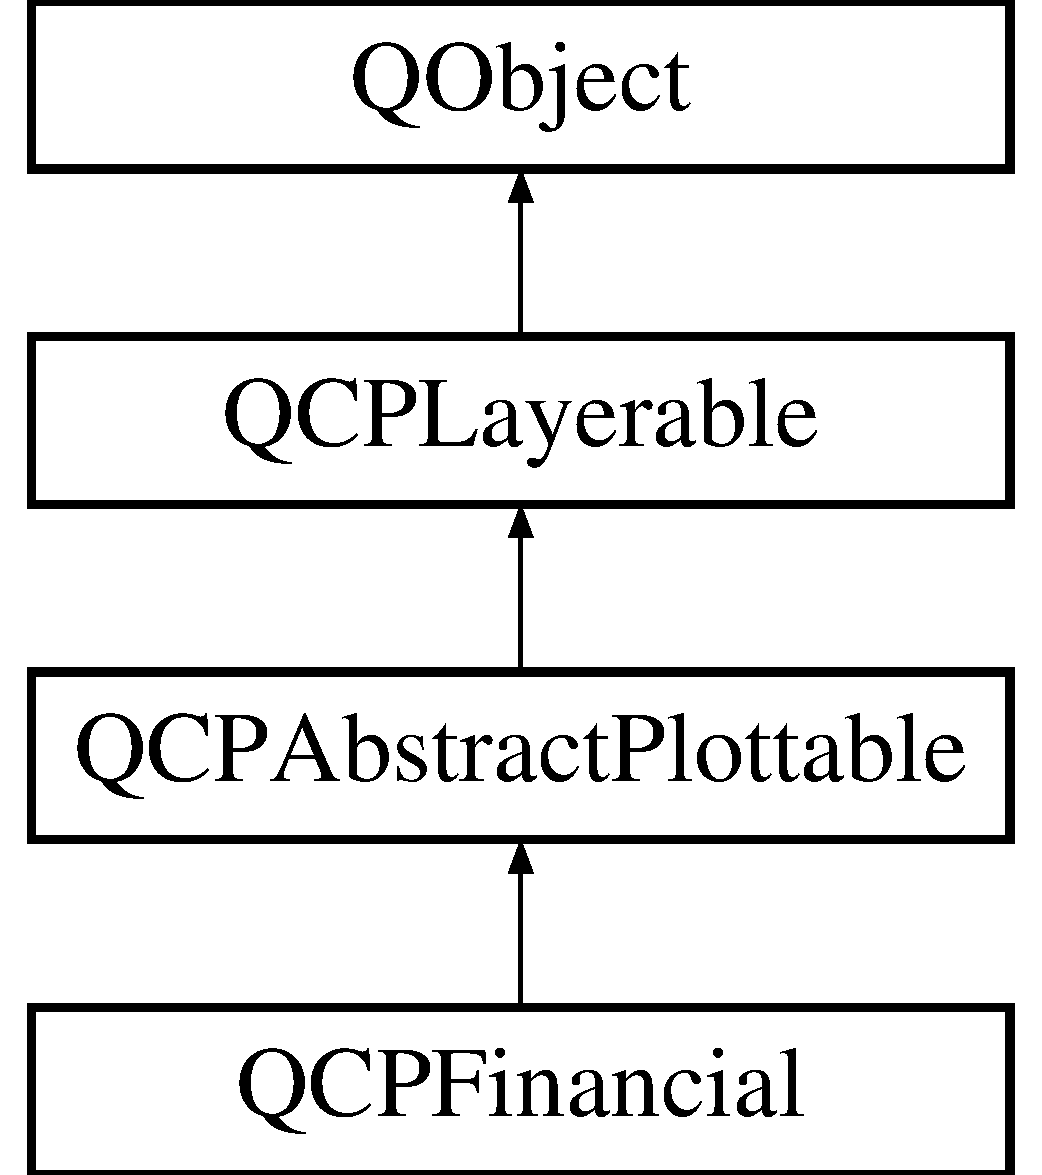
\includegraphics[height=4.000000cm]{class_q_c_p_financial}
\end{center}
\end{figure}
\subsection*{Public Types}
\begin{DoxyCompactItemize}
\item 
enum \hyperlink{class_q_c_p_financial_a0f800e21ee98d646dfc6f8f89d10ebfb}{Chart\+Style} \{ \hyperlink{class_q_c_p_financial_a0f800e21ee98d646dfc6f8f89d10ebfba3a516016c9298d3e95dd82aa203c4390}{cs\+Ohlc}, 
\hyperlink{class_q_c_p_financial_a0f800e21ee98d646dfc6f8f89d10ebfbac803cbd39f26e3f206bcc7028679e62f}{cs\+Candlestick}
 \}
\end{DoxyCompactItemize}
\subsection*{Public Member Functions}
\begin{DoxyCompactItemize}
\item 
\hyperlink{class_q_c_p_financial_a4702d5248feeb9d1ec6e3ce725b10b32}{Q\+C\+P\+Financial} (\hyperlink{class_q_c_p_axis}{Q\+C\+P\+Axis} $\ast$key\+Axis, \hyperlink{class_q_c_p_axis}{Q\+C\+P\+Axis} $\ast$value\+Axis)
\item 
\hyperlink{qcustomplot_8h_a745c09823fae0974b50beca9bc3b3d7d}{Q\+C\+P\+Financial\+Data\+Map} $\ast$ \hyperlink{class_q_c_p_financial_a528c81578e4f25999a9169127763cfd4}{data} () const
\item 
\hypertarget{class_q_c_p_financial_a5243371c1fde30fdae00555d7760ec2d}{}\label{class_q_c_p_financial_a5243371c1fde30fdae00555d7760ec2d} 
\hyperlink{class_q_c_p_financial_a0f800e21ee98d646dfc6f8f89d10ebfb}{Chart\+Style} {\bfseries chart\+Style} () const
\item 
\hypertarget{class_q_c_p_financial_a12548f13658eda5833204ef60f524870}{}\label{class_q_c_p_financial_a12548f13658eda5833204ef60f524870} 
double {\bfseries width} () const
\item 
\hypertarget{class_q_c_p_financial_afd4b51de5be8e53776b649f9877a50e6}{}\label{class_q_c_p_financial_afd4b51de5be8e53776b649f9877a50e6} 
bool {\bfseries two\+Colored} () const
\item 
\hypertarget{class_q_c_p_financial_ae922e75f3d5b8854369ac0bf1ebfb053}{}\label{class_q_c_p_financial_ae922e75f3d5b8854369ac0bf1ebfb053} 
Q\+Brush {\bfseries brush\+Positive} () const
\item 
\hypertarget{class_q_c_p_financial_ad4fdc5bc21f5eb17070e043bd4a35f53}{}\label{class_q_c_p_financial_ad4fdc5bc21f5eb17070e043bd4a35f53} 
Q\+Brush {\bfseries brush\+Negative} () const
\item 
\hypertarget{class_q_c_p_financial_ae803fe25fdd6f0acacde4539590795ed}{}\label{class_q_c_p_financial_ae803fe25fdd6f0acacde4539590795ed} 
Q\+Pen {\bfseries pen\+Positive} () const
\item 
\hypertarget{class_q_c_p_financial_a25d9a8f256e5ddcba56b6e2e7e968653}{}\label{class_q_c_p_financial_a25d9a8f256e5ddcba56b6e2e7e968653} 
Q\+Pen {\bfseries pen\+Negative} () const
\item 
void \hyperlink{class_q_c_p_financial_adf12a86082f1e488df6a4e8603f8fd6d}{set\+Data} (\hyperlink{qcustomplot_8h_a745c09823fae0974b50beca9bc3b3d7d}{Q\+C\+P\+Financial\+Data\+Map} $\ast$\hyperlink{class_q_c_p_financial_a528c81578e4f25999a9169127763cfd4}{data}, bool copy=false)
\item 
void \hyperlink{class_q_c_p_financial_a886881339d6447432af55adaad748c3c}{set\+Data} (const Q\+Vector$<$ double $>$ \&key, const Q\+Vector$<$ double $>$ \&open, const Q\+Vector$<$ double $>$ \&high, const Q\+Vector$<$ double $>$ \&low, const Q\+Vector$<$ double $>$ \&close)
\item 
void \hyperlink{class_q_c_p_financial_a5a59175d36279d71596e64d7bb65596f}{set\+Chart\+Style} (\hyperlink{class_q_c_p_financial_a0f800e21ee98d646dfc6f8f89d10ebfb}{Chart\+Style} style)
\item 
void \hyperlink{class_q_c_p_financial_a99633f8bac86a61d534ae5eeb1a3068f}{set\+Width} (double width)
\item 
void \hyperlink{class_q_c_p_financial_a138e44aac160a17a9676652e240c5f08}{set\+Two\+Colored} (bool two\+Colored)
\item 
void \hyperlink{class_q_c_p_financial_a5ebff2b1764efd07cc44942e67821829}{set\+Brush\+Positive} (const Q\+Brush \&brush)
\item 
void \hyperlink{class_q_c_p_financial_a8bbdd87629f9144b3ef51af660c0961a}{set\+Brush\+Negative} (const Q\+Brush \&brush)
\item 
void \hyperlink{class_q_c_p_financial_ac58aa3adc7a35aab0088764b840683e5}{set\+Pen\+Positive} (const Q\+Pen \&pen)
\item 
void \hyperlink{class_q_c_p_financial_afe5c07e94ccea01a75b3a2476993c346}{set\+Pen\+Negative} (const Q\+Pen \&pen)
\item 
void \hyperlink{class_q_c_p_financial_a1a83396f97fcc68f2b7aa8d9782feffe}{add\+Data} (const \hyperlink{qcustomplot_8h_a745c09823fae0974b50beca9bc3b3d7d}{Q\+C\+P\+Financial\+Data\+Map} \&data\+Map)
\item 
void \hyperlink{class_q_c_p_financial_a3b6144b48a6a8e63236fc5bf70d40c00}{add\+Data} (const \hyperlink{class_q_c_p_financial_data}{Q\+C\+P\+Financial\+Data} \&\hyperlink{class_q_c_p_financial_a528c81578e4f25999a9169127763cfd4}{data})
\item 
void \hyperlink{class_q_c_p_financial_a688bbd052e00a02954ddb0068b378170}{add\+Data} (double key, double open, double high, double low, double close)
\item 
void \hyperlink{class_q_c_p_financial_aa1abe3bdafb297497f09cdbdc4db3958}{add\+Data} (const Q\+Vector$<$ double $>$ \&key, const Q\+Vector$<$ double $>$ \&open, const Q\+Vector$<$ double $>$ \&high, const Q\+Vector$<$ double $>$ \&low, const Q\+Vector$<$ double $>$ \&close)
\item 
void \hyperlink{class_q_c_p_financial_a097c0383c7c1e9042ca7f93cb439d15a}{remove\+Data\+Before} (double key)
\item 
void \hyperlink{class_q_c_p_financial_aa0fcd357005288c833a230c7874825ba}{remove\+Data\+After} (double key)
\item 
void \hyperlink{class_q_c_p_financial_a048c741d3c8cc5709c2c44b759fdf27c}{remove\+Data} (double from\+Key, double to\+Key)
\item 
void \hyperlink{class_q_c_p_financial_ae527d8a11290906b083d1ab598c380ea}{remove\+Data} (double key)
\item 
virtual void \hyperlink{class_q_c_p_financial_a11fd49928c33e55e27b7319c6927864a}{clear\+Data} ()
\item 
virtual double \hyperlink{class_q_c_p_financial_a77bffad8f3fcbcccbef03ead1c538e3a}{select\+Test} (const Q\+PointF \&pos, bool only\+Selectable, Q\+Variant $\ast$details=0) const
\end{DoxyCompactItemize}
\subsection*{Static Public Member Functions}
\begin{DoxyCompactItemize}
\item 
static \hyperlink{qcustomplot_8h_a745c09823fae0974b50beca9bc3b3d7d}{Q\+C\+P\+Financial\+Data\+Map} \hyperlink{class_q_c_p_financial_a0c3453d1c03e320950fdd2df54e3ebc8}{time\+Series\+To\+Ohlc} (const Q\+Vector$<$ double $>$ \&time, const Q\+Vector$<$ double $>$ \&value, double time\+Bin\+Size, double time\+Bin\+Offset=0)
\end{DoxyCompactItemize}
\subsection*{Protected Member Functions}
\begin{DoxyCompactItemize}
\item 
\hypertarget{class_q_c_p_financial_ad71a59a1b42616594831e04e52c92120}{}\label{class_q_c_p_financial_ad71a59a1b42616594831e04e52c92120} 
virtual void {\bfseries draw} (\hyperlink{class_q_c_p_painter}{Q\+C\+P\+Painter} $\ast$painter)
\item 
\hypertarget{class_q_c_p_financial_a474a3994b081892f1dbdd1162e055b96}{}\label{class_q_c_p_financial_a474a3994b081892f1dbdd1162e055b96} 
virtual void {\bfseries draw\+Legend\+Icon} (\hyperlink{class_q_c_p_painter}{Q\+C\+P\+Painter} $\ast$painter, const Q\+RectF \&rect) const
\item 
\hypertarget{class_q_c_p_financial_a13da88ffd42ad192a672d54f3f233d15}{}\label{class_q_c_p_financial_a13da88ffd42ad192a672d54f3f233d15} 
virtual \hyperlink{class_q_c_p_range}{Q\+C\+P\+Range} {\bfseries get\+Key\+Range} (bool \&found\+Range, \hyperlink{class_q_c_p_abstract_plottable_a661743478a1d3c09d28ec2711d7653d8}{Sign\+Domain} in\+Sign\+Domain=\hyperlink{class_q_c_p_abstract_plottable_a661743478a1d3c09d28ec2711d7653d8a082b98cfb91a7363a3b5cd17b0c1cd60}{sd\+Both}) const
\item 
\hypertarget{class_q_c_p_financial_a91c698076647d58223f49e7248d1487e}{}\label{class_q_c_p_financial_a91c698076647d58223f49e7248d1487e} 
virtual \hyperlink{class_q_c_p_range}{Q\+C\+P\+Range} {\bfseries get\+Value\+Range} (bool \&found\+Range, \hyperlink{class_q_c_p_abstract_plottable_a661743478a1d3c09d28ec2711d7653d8}{Sign\+Domain} in\+Sign\+Domain=\hyperlink{class_q_c_p_abstract_plottable_a661743478a1d3c09d28ec2711d7653d8a082b98cfb91a7363a3b5cd17b0c1cd60}{sd\+Both}) const
\item 
\hypertarget{class_q_c_p_financial_a3c3007a7434e29d042c77ccf4f497e66}{}\label{class_q_c_p_financial_a3c3007a7434e29d042c77ccf4f497e66} 
void {\bfseries draw\+Ohlc\+Plot} (\hyperlink{class_q_c_p_painter}{Q\+C\+P\+Painter} $\ast$painter, const Q\+C\+P\+Financial\+Data\+Map\+::const\+\_\+iterator \&begin, const Q\+C\+P\+Financial\+Data\+Map\+::const\+\_\+iterator \&end)
\item 
\hypertarget{class_q_c_p_financial_a71f5081da0e5ab9c40a488ad40cff122}{}\label{class_q_c_p_financial_a71f5081da0e5ab9c40a488ad40cff122} 
void {\bfseries draw\+Candlestick\+Plot} (\hyperlink{class_q_c_p_painter}{Q\+C\+P\+Painter} $\ast$painter, const Q\+C\+P\+Financial\+Data\+Map\+::const\+\_\+iterator \&begin, const Q\+C\+P\+Financial\+Data\+Map\+::const\+\_\+iterator \&end)
\item 
\hypertarget{class_q_c_p_financial_a9df2d86e6ad3b58b51798d720e0f4739}{}\label{class_q_c_p_financial_a9df2d86e6ad3b58b51798d720e0f4739} 
double {\bfseries ohlc\+Select\+Test} (const Q\+PointF \&pos, const Q\+C\+P\+Financial\+Data\+Map\+::const\+\_\+iterator \&begin, const Q\+C\+P\+Financial\+Data\+Map\+::const\+\_\+iterator \&end) const
\item 
\hypertarget{class_q_c_p_financial_a6fa1e18f18b37d3a0502b97d864a6d15}{}\label{class_q_c_p_financial_a6fa1e18f18b37d3a0502b97d864a6d15} 
double {\bfseries candlestick\+Select\+Test} (const Q\+PointF \&pos, const Q\+C\+P\+Financial\+Data\+Map\+::const\+\_\+iterator \&begin, const Q\+C\+P\+Financial\+Data\+Map\+::const\+\_\+iterator \&end) const
\item 
\hypertarget{class_q_c_p_financial_ab74167a55319771c5da0e06406c2c2f2}{}\label{class_q_c_p_financial_ab74167a55319771c5da0e06406c2c2f2} 
void {\bfseries get\+Visible\+Data\+Bounds} (Q\+C\+P\+Financial\+Data\+Map\+::const\+\_\+iterator \&lower, Q\+C\+P\+Financial\+Data\+Map\+::const\+\_\+iterator \&upper) const
\end{DoxyCompactItemize}
\subsection*{Protected Attributes}
\begin{DoxyCompactItemize}
\item 
\hypertarget{class_q_c_p_financial_a475f63587ca1077d8c30aaf2b71ae026}{}\label{class_q_c_p_financial_a475f63587ca1077d8c30aaf2b71ae026} 
\hyperlink{qcustomplot_8h_a745c09823fae0974b50beca9bc3b3d7d}{Q\+C\+P\+Financial\+Data\+Map} $\ast$ {\bfseries m\+Data}
\item 
\hypertarget{class_q_c_p_financial_ab65c2ce8d6354451870bb44b894c1e92}{}\label{class_q_c_p_financial_ab65c2ce8d6354451870bb44b894c1e92} 
\hyperlink{class_q_c_p_financial_a0f800e21ee98d646dfc6f8f89d10ebfb}{Chart\+Style} {\bfseries m\+Chart\+Style}
\item 
\hypertarget{class_q_c_p_financial_af630e5eb8485146b9c777e63fd1cf993}{}\label{class_q_c_p_financial_af630e5eb8485146b9c777e63fd1cf993} 
double {\bfseries m\+Width}
\item 
\hypertarget{class_q_c_p_financial_a6afe919190b884d9bac026cefcc8c0a8}{}\label{class_q_c_p_financial_a6afe919190b884d9bac026cefcc8c0a8} 
bool {\bfseries m\+Two\+Colored}
\item 
\hypertarget{class_q_c_p_financial_ab7e6eed16260a2f88ca6bd940dffea79}{}\label{class_q_c_p_financial_ab7e6eed16260a2f88ca6bd940dffea79} 
Q\+Brush {\bfseries m\+Brush\+Positive}
\item 
\hypertarget{class_q_c_p_financial_acb0e31874b7a1deb56bd42e8ab3e68f2}{}\label{class_q_c_p_financial_acb0e31874b7a1deb56bd42e8ab3e68f2} 
Q\+Brush {\bfseries m\+Brush\+Negative}
\item 
\hypertarget{class_q_c_p_financial_aa6599186f417ba615caebb3f6c762bd8}{}\label{class_q_c_p_financial_aa6599186f417ba615caebb3f6c762bd8} 
Q\+Pen {\bfseries m\+Pen\+Positive}
\item 
\hypertarget{class_q_c_p_financial_a263fbfefde2cc19c8d4024a8319c2bbb}{}\label{class_q_c_p_financial_a263fbfefde2cc19c8d4024a8319c2bbb} 
Q\+Pen {\bfseries m\+Pen\+Negative}
\end{DoxyCompactItemize}
\subsection*{Friends}
\begin{DoxyCompactItemize}
\item 
\hypertarget{class_q_c_p_financial_a1cdf9df76adcfae45261690aa0ca2198}{}\label{class_q_c_p_financial_a1cdf9df76adcfae45261690aa0ca2198} 
class {\bfseries Q\+Custom\+Plot}
\item 
\hypertarget{class_q_c_p_financial_a8429035e7adfbd7f05805a6530ad5e3b}{}\label{class_q_c_p_financial_a8429035e7adfbd7f05805a6530ad5e3b} 
class {\bfseries Q\+C\+P\+Legend}
\end{DoxyCompactItemize}
\subsection*{Additional Inherited Members}


\subsection{Detailed Description}
A plottable representing a financial stock chart. 



This plottable represents time series data binned to certain intervals, mainly used for stock charts. The two common representations O\+H\+LC (Open-\/\+High-\/\+Low-\/\+Close) bars and Candlesticks can be set via \hyperlink{class_q_c_p_financial_a5a59175d36279d71596e64d7bb65596f}{set\+Chart\+Style}.

The data is passed via \hyperlink{class_q_c_p_financial_adf12a86082f1e488df6a4e8603f8fd6d}{set\+Data} as a set of open/high/low/close values at certain keys (typically times). This means the data must be already binned appropriately. If data is only available as a series of values (e.\+g. {\itshape price} against {\itshape time}), you can use the static convenience function \hyperlink{class_q_c_p_financial_a0c3453d1c03e320950fdd2df54e3ebc8}{time\+Series\+To\+Ohlc} to generate binned O\+H\+L\+C-\/data which can then be passed to \hyperlink{class_q_c_p_financial_adf12a86082f1e488df6a4e8603f8fd6d}{set\+Data}.

The width of the O\+H\+LC bars/candlesticks can be controlled with \hyperlink{class_q_c_p_financial_a99633f8bac86a61d534ae5eeb1a3068f}{set\+Width} and is given in plot key coordinates. A typical choice is to set it to (or slightly less than) one bin interval width.\hypertarget{class_q_c_p_statistical_box_appearance}{}\subsection{Changing the appearance}\label{class_q_c_p_statistical_box_appearance}
Charts can be either single-\/ or two-\/colored (\hyperlink{class_q_c_p_financial_a138e44aac160a17a9676652e240c5f08}{set\+Two\+Colored}). If set to be single-\/colored, lines are drawn with the plottable\textquotesingle{}s pen (\hyperlink{class_q_c_p_abstract_plottable_ab74b09ae4c0e7e13142fe4b5bf46cac7}{set\+Pen}) and fills with the brush (\hyperlink{class_q_c_p_abstract_plottable_a7a4b92144dca6453a1f0f210e27edc74}{set\+Brush}).

If set to two-\/colored, positive changes of the value during an interval ({\itshape close} $>$= {\itshape open}) are represented with a different pen and brush than negative changes ({\itshape close} $<$ {\itshape open}). These can be configured with \hyperlink{class_q_c_p_financial_ac58aa3adc7a35aab0088764b840683e5}{set\+Pen\+Positive}, \hyperlink{class_q_c_p_financial_afe5c07e94ccea01a75b3a2476993c346}{set\+Pen\+Negative}, \hyperlink{class_q_c_p_financial_a5ebff2b1764efd07cc44942e67821829}{set\+Brush\+Positive}, and \hyperlink{class_q_c_p_financial_a8bbdd87629f9144b3ef51af660c0961a}{set\+Brush\+Negative}. In two-\/colored mode, the normal plottable pen/brush is ignored. Upon selection however, the normal selected pen/brush (\hyperlink{class_q_c_p_abstract_plottable_a6911603cad23ab0469b108224517516f}{set\+Selected\+Pen}, \hyperlink{class_q_c_p_abstract_plottable_ae8c816874089f7a44001e8618e81a9dc}{set\+Selected\+Brush}) is used, irrespective of whether the chart is single-\/ or two-\/colored. 

\subsection{Member Enumeration Documentation}
\hypertarget{class_q_c_p_financial_a0f800e21ee98d646dfc6f8f89d10ebfb}{}\label{class_q_c_p_financial_a0f800e21ee98d646dfc6f8f89d10ebfb} 
\index{Q\+C\+P\+Financial@{Q\+C\+P\+Financial}!Chart\+Style@{Chart\+Style}}
\index{Chart\+Style@{Chart\+Style}!Q\+C\+P\+Financial@{Q\+C\+P\+Financial}}
\subsubsection{\texorpdfstring{Chart\+Style}{ChartStyle}}
{\footnotesize\ttfamily enum \hyperlink{class_q_c_p_financial_a0f800e21ee98d646dfc6f8f89d10ebfb}{Q\+C\+P\+Financial\+::\+Chart\+Style}}

Defines the possible representations of O\+H\+LC data in the plot.

\begin{DoxySeeAlso}{See also}
\hyperlink{class_q_c_p_financial_a5a59175d36279d71596e64d7bb65596f}{set\+Chart\+Style} 
\end{DoxySeeAlso}
\begin{DoxyEnumFields}{Enumerator}
\raisebox{\heightof{T}}[0pt][0pt]{\index{cs\+Ohlc@{cs\+Ohlc}!Q\+C\+P\+Financial@{Q\+C\+P\+Financial}}\index{Q\+C\+P\+Financial@{Q\+C\+P\+Financial}!cs\+Ohlc@{cs\+Ohlc}}}\hypertarget{class_q_c_p_financial_a0f800e21ee98d646dfc6f8f89d10ebfba3a516016c9298d3e95dd82aa203c4390}{}\label{class_q_c_p_financial_a0f800e21ee98d646dfc6f8f89d10ebfba3a516016c9298d3e95dd82aa203c4390} 
cs\+Ohlc&Open-\/\+High-\/\+Low-\/\+Close bar representation. \\
\hline

\raisebox{\heightof{T}}[0pt][0pt]{\index{cs\+Candlestick@{cs\+Candlestick}!Q\+C\+P\+Financial@{Q\+C\+P\+Financial}}\index{Q\+C\+P\+Financial@{Q\+C\+P\+Financial}!cs\+Candlestick@{cs\+Candlestick}}}\hypertarget{class_q_c_p_financial_a0f800e21ee98d646dfc6f8f89d10ebfbac803cbd39f26e3f206bcc7028679e62f}{}\label{class_q_c_p_financial_a0f800e21ee98d646dfc6f8f89d10ebfbac803cbd39f26e3f206bcc7028679e62f} 
cs\+Candlestick&Candlestick representation. \\
\hline

\end{DoxyEnumFields}


\subsection{Constructor \& Destructor Documentation}
\hypertarget{class_q_c_p_financial_a4702d5248feeb9d1ec6e3ce725b10b32}{}\label{class_q_c_p_financial_a4702d5248feeb9d1ec6e3ce725b10b32} 
\index{Q\+C\+P\+Financial@{Q\+C\+P\+Financial}!Q\+C\+P\+Financial@{Q\+C\+P\+Financial}}
\index{Q\+C\+P\+Financial@{Q\+C\+P\+Financial}!Q\+C\+P\+Financial@{Q\+C\+P\+Financial}}
\subsubsection{\texorpdfstring{Q\+C\+P\+Financial()}{QCPFinancial()}}
{\footnotesize\ttfamily Q\+C\+P\+Financial\+::\+Q\+C\+P\+Financial (\begin{DoxyParamCaption}\item[{\hyperlink{class_q_c_p_axis}{Q\+C\+P\+Axis} $\ast$}]{key\+Axis,  }\item[{\hyperlink{class_q_c_p_axis}{Q\+C\+P\+Axis} $\ast$}]{value\+Axis }\end{DoxyParamCaption})\hspace{0.3cm}{\ttfamily [explicit]}}

Constructs a financial chart which uses {\itshape key\+Axis} as its key axis (\char`\"{}x\char`\"{}) and {\itshape value\+Axis} as its value axis (\char`\"{}y\char`\"{}). {\itshape key\+Axis} and {\itshape value\+Axis} must reside in the same \hyperlink{class_q_custom_plot}{Q\+Custom\+Plot} instance and not have the same orientation. If either of these restrictions is violated, a corresponding message is printed to the debug output (q\+Debug), the construction is not aborted, though.

The constructed \hyperlink{class_q_c_p_financial}{Q\+C\+P\+Financial} can be added to the plot with \hyperlink{class_q_custom_plot_ab7ad9174f701f9c6f64e378df77927a6}{Q\+Custom\+Plot\+::add\+Plottable}, \hyperlink{class_q_custom_plot}{Q\+Custom\+Plot} then takes ownership of the financial chart. 

\subsection{Member Function Documentation}
\hypertarget{class_q_c_p_financial_a1a83396f97fcc68f2b7aa8d9782feffe}{}\label{class_q_c_p_financial_a1a83396f97fcc68f2b7aa8d9782feffe} 
\index{Q\+C\+P\+Financial@{Q\+C\+P\+Financial}!add\+Data@{add\+Data}}
\index{add\+Data@{add\+Data}!Q\+C\+P\+Financial@{Q\+C\+P\+Financial}}
\subsubsection{\texorpdfstring{add\+Data()}{addData()}\hspace{0.1cm}{\footnotesize\ttfamily [1/4]}}
{\footnotesize\ttfamily void Q\+C\+P\+Financial\+::add\+Data (\begin{DoxyParamCaption}\item[{const \hyperlink{qcustomplot_8h_a745c09823fae0974b50beca9bc3b3d7d}{Q\+C\+P\+Financial\+Data\+Map} \&}]{data\+Map }\end{DoxyParamCaption})}

Adds the provided data points in {\itshape data\+Map} to the current data.

Alternatively, you can also access and modify the data via the \hyperlink{class_q_c_p_financial_a528c81578e4f25999a9169127763cfd4}{data} method, which returns a pointer to the internal \hyperlink{qcustomplot_8h_a745c09823fae0974b50beca9bc3b3d7d}{Q\+C\+P\+Financial\+Data\+Map}.

\begin{DoxySeeAlso}{See also}
\hyperlink{class_q_c_p_financial_a048c741d3c8cc5709c2c44b759fdf27c}{remove\+Data} 
\end{DoxySeeAlso}
\hypertarget{class_q_c_p_financial_a3b6144b48a6a8e63236fc5bf70d40c00}{}\label{class_q_c_p_financial_a3b6144b48a6a8e63236fc5bf70d40c00} 
\index{Q\+C\+P\+Financial@{Q\+C\+P\+Financial}!add\+Data@{add\+Data}}
\index{add\+Data@{add\+Data}!Q\+C\+P\+Financial@{Q\+C\+P\+Financial}}
\subsubsection{\texorpdfstring{add\+Data()}{addData()}\hspace{0.1cm}{\footnotesize\ttfamily [2/4]}}
{\footnotesize\ttfamily void Q\+C\+P\+Financial\+::add\+Data (\begin{DoxyParamCaption}\item[{const \hyperlink{class_q_c_p_financial_data}{Q\+C\+P\+Financial\+Data} \&}]{data }\end{DoxyParamCaption})}

This is an overloaded member function, provided for convenience. It differs from the above function only in what argument(s) it accepts.

Adds the provided single data point in {\itshape data} to the current data.

Alternatively, you can also access and modify the data via the \hyperlink{class_q_c_p_financial_a528c81578e4f25999a9169127763cfd4}{data} method, which returns a pointer to the internal \hyperlink{class_q_c_p_financial_data}{Q\+C\+P\+Financial\+Data}.

\begin{DoxySeeAlso}{See also}
\hyperlink{class_q_c_p_financial_a048c741d3c8cc5709c2c44b759fdf27c}{remove\+Data} 
\end{DoxySeeAlso}
\hypertarget{class_q_c_p_financial_a688bbd052e00a02954ddb0068b378170}{}\label{class_q_c_p_financial_a688bbd052e00a02954ddb0068b378170} 
\index{Q\+C\+P\+Financial@{Q\+C\+P\+Financial}!add\+Data@{add\+Data}}
\index{add\+Data@{add\+Data}!Q\+C\+P\+Financial@{Q\+C\+P\+Financial}}
\subsubsection{\texorpdfstring{add\+Data()}{addData()}\hspace{0.1cm}{\footnotesize\ttfamily [3/4]}}
{\footnotesize\ttfamily void Q\+C\+P\+Financial\+::add\+Data (\begin{DoxyParamCaption}\item[{double}]{key,  }\item[{double}]{open,  }\item[{double}]{high,  }\item[{double}]{low,  }\item[{double}]{close }\end{DoxyParamCaption})}

This is an overloaded member function, provided for convenience. It differs from the above function only in what argument(s) it accepts.

Adds the provided single data point given by {\itshape key}, {\itshape open}, {\itshape high}, {\itshape low}, and {\itshape close} to the current data.

Alternatively, you can also access and modify the data via the \hyperlink{class_q_c_p_financial_a528c81578e4f25999a9169127763cfd4}{data} method, which returns a pointer to the internal \hyperlink{class_q_c_p_financial_data}{Q\+C\+P\+Financial\+Data}.

\begin{DoxySeeAlso}{See also}
\hyperlink{class_q_c_p_financial_a048c741d3c8cc5709c2c44b759fdf27c}{remove\+Data} 
\end{DoxySeeAlso}
\hypertarget{class_q_c_p_financial_aa1abe3bdafb297497f09cdbdc4db3958}{}\label{class_q_c_p_financial_aa1abe3bdafb297497f09cdbdc4db3958} 
\index{Q\+C\+P\+Financial@{Q\+C\+P\+Financial}!add\+Data@{add\+Data}}
\index{add\+Data@{add\+Data}!Q\+C\+P\+Financial@{Q\+C\+P\+Financial}}
\subsubsection{\texorpdfstring{add\+Data()}{addData()}\hspace{0.1cm}{\footnotesize\ttfamily [4/4]}}
{\footnotesize\ttfamily void Q\+C\+P\+Financial\+::add\+Data (\begin{DoxyParamCaption}\item[{const Q\+Vector$<$ double $>$ \&}]{key,  }\item[{const Q\+Vector$<$ double $>$ \&}]{open,  }\item[{const Q\+Vector$<$ double $>$ \&}]{high,  }\item[{const Q\+Vector$<$ double $>$ \&}]{low,  }\item[{const Q\+Vector$<$ double $>$ \&}]{close }\end{DoxyParamCaption})}

This is an overloaded member function, provided for convenience. It differs from the above function only in what argument(s) it accepts.

Adds the provided open/high/low/close data to the current data.

Alternatively, you can also access and modify the data via the \hyperlink{class_q_c_p_financial_a528c81578e4f25999a9169127763cfd4}{data} method, which returns a pointer to the internal \hyperlink{class_q_c_p_financial_data}{Q\+C\+P\+Financial\+Data}.

\begin{DoxySeeAlso}{See also}
\hyperlink{class_q_c_p_financial_a048c741d3c8cc5709c2c44b759fdf27c}{remove\+Data} 
\end{DoxySeeAlso}
\hypertarget{class_q_c_p_financial_a11fd49928c33e55e27b7319c6927864a}{}\label{class_q_c_p_financial_a11fd49928c33e55e27b7319c6927864a} 
\index{Q\+C\+P\+Financial@{Q\+C\+P\+Financial}!clear\+Data@{clear\+Data}}
\index{clear\+Data@{clear\+Data}!Q\+C\+P\+Financial@{Q\+C\+P\+Financial}}
\subsubsection{\texorpdfstring{clear\+Data()}{clearData()}}
{\footnotesize\ttfamily void Q\+C\+P\+Financial\+::clear\+Data (\begin{DoxyParamCaption}{ }\end{DoxyParamCaption})\hspace{0.3cm}{\ttfamily [virtual]}}

Removes all data points.

\begin{DoxySeeAlso}{See also}
\hyperlink{class_q_c_p_financial_a048c741d3c8cc5709c2c44b759fdf27c}{remove\+Data}, \hyperlink{class_q_c_p_financial_aa0fcd357005288c833a230c7874825ba}{remove\+Data\+After}, \hyperlink{class_q_c_p_financial_a097c0383c7c1e9042ca7f93cb439d15a}{remove\+Data\+Before} 
\end{DoxySeeAlso}


Implements \hyperlink{class_q_c_p_abstract_plottable_a86e5b8fd4b6ff4f4084e7ea4c573fc53}{Q\+C\+P\+Abstract\+Plottable}.

\hypertarget{class_q_c_p_financial_a528c81578e4f25999a9169127763cfd4}{}\label{class_q_c_p_financial_a528c81578e4f25999a9169127763cfd4} 
\index{Q\+C\+P\+Financial@{Q\+C\+P\+Financial}!data@{data}}
\index{data@{data}!Q\+C\+P\+Financial@{Q\+C\+P\+Financial}}
\subsubsection{\texorpdfstring{data()}{data()}}
{\footnotesize\ttfamily \hyperlink{qcustomplot_8h_a745c09823fae0974b50beca9bc3b3d7d}{Q\+C\+P\+Financial\+Data\+Map} $\ast$ Q\+C\+P\+Financial\+::data (\begin{DoxyParamCaption}{ }\end{DoxyParamCaption}) const\hspace{0.3cm}{\ttfamily [inline]}}

Returns a pointer to the internal data storage of type \hyperlink{qcustomplot_8h_a745c09823fae0974b50beca9bc3b3d7d}{Q\+C\+P\+Financial\+Data\+Map}. You may use it to directly manipulate the data, which may be more convenient and faster than using the regular \hyperlink{class_q_c_p_financial_adf12a86082f1e488df6a4e8603f8fd6d}{set\+Data} or \hyperlink{class_q_c_p_financial_a1a83396f97fcc68f2b7aa8d9782feffe}{add\+Data} methods, in certain situations. \hypertarget{class_q_c_p_financial_a048c741d3c8cc5709c2c44b759fdf27c}{}\label{class_q_c_p_financial_a048c741d3c8cc5709c2c44b759fdf27c} 
\index{Q\+C\+P\+Financial@{Q\+C\+P\+Financial}!remove\+Data@{remove\+Data}}
\index{remove\+Data@{remove\+Data}!Q\+C\+P\+Financial@{Q\+C\+P\+Financial}}
\subsubsection{\texorpdfstring{remove\+Data()}{removeData()}\hspace{0.1cm}{\footnotesize\ttfamily [1/2]}}
{\footnotesize\ttfamily void Q\+C\+P\+Financial\+::remove\+Data (\begin{DoxyParamCaption}\item[{double}]{from\+Key,  }\item[{double}]{to\+Key }\end{DoxyParamCaption})}

Removes all data points with keys between {\itshape from\+Key} and {\itshape to\+Key}. if {\itshape from\+Key} is greater or equal to {\itshape to\+Key}, the function does nothing. To remove a single data point with known key, use \hyperlink{class_q_c_p_financial_ae527d8a11290906b083d1ab598c380ea}{remove\+Data(double key)}.

\begin{DoxySeeAlso}{See also}
\hyperlink{class_q_c_p_financial_a1a83396f97fcc68f2b7aa8d9782feffe}{add\+Data}, \hyperlink{class_q_c_p_financial_a11fd49928c33e55e27b7319c6927864a}{clear\+Data} 
\end{DoxySeeAlso}
\hypertarget{class_q_c_p_financial_ae527d8a11290906b083d1ab598c380ea}{}\label{class_q_c_p_financial_ae527d8a11290906b083d1ab598c380ea} 
\index{Q\+C\+P\+Financial@{Q\+C\+P\+Financial}!remove\+Data@{remove\+Data}}
\index{remove\+Data@{remove\+Data}!Q\+C\+P\+Financial@{Q\+C\+P\+Financial}}
\subsubsection{\texorpdfstring{remove\+Data()}{removeData()}\hspace{0.1cm}{\footnotesize\ttfamily [2/2]}}
{\footnotesize\ttfamily void Q\+C\+P\+Financial\+::remove\+Data (\begin{DoxyParamCaption}\item[{double}]{key }\end{DoxyParamCaption})}

This is an overloaded member function, provided for convenience. It differs from the above function only in what argument(s) it accepts.

Removes a single data point at {\itshape key}. If the position is not known with absolute precision, consider using \hyperlink{class_q_c_p_financial_a048c741d3c8cc5709c2c44b759fdf27c}{remove\+Data(double from\+Key, double to\+Key)} with a small fuzziness interval around the suspected position, depeding on the precision with which the key is known.

\begin{DoxySeeAlso}{See also}
\hyperlink{class_q_c_p_financial_a1a83396f97fcc68f2b7aa8d9782feffe}{add\+Data}, \hyperlink{class_q_c_p_financial_a11fd49928c33e55e27b7319c6927864a}{clear\+Data} 
\end{DoxySeeAlso}
\hypertarget{class_q_c_p_financial_aa0fcd357005288c833a230c7874825ba}{}\label{class_q_c_p_financial_aa0fcd357005288c833a230c7874825ba} 
\index{Q\+C\+P\+Financial@{Q\+C\+P\+Financial}!remove\+Data\+After@{remove\+Data\+After}}
\index{remove\+Data\+After@{remove\+Data\+After}!Q\+C\+P\+Financial@{Q\+C\+P\+Financial}}
\subsubsection{\texorpdfstring{remove\+Data\+After()}{removeDataAfter()}}
{\footnotesize\ttfamily void Q\+C\+P\+Financial\+::remove\+Data\+After (\begin{DoxyParamCaption}\item[{double}]{key }\end{DoxyParamCaption})}

Removes all data points with keys greater than {\itshape key}.

\begin{DoxySeeAlso}{See also}
\hyperlink{class_q_c_p_financial_a1a83396f97fcc68f2b7aa8d9782feffe}{add\+Data}, \hyperlink{class_q_c_p_financial_a11fd49928c33e55e27b7319c6927864a}{clear\+Data} 
\end{DoxySeeAlso}
\hypertarget{class_q_c_p_financial_a097c0383c7c1e9042ca7f93cb439d15a}{}\label{class_q_c_p_financial_a097c0383c7c1e9042ca7f93cb439d15a} 
\index{Q\+C\+P\+Financial@{Q\+C\+P\+Financial}!remove\+Data\+Before@{remove\+Data\+Before}}
\index{remove\+Data\+Before@{remove\+Data\+Before}!Q\+C\+P\+Financial@{Q\+C\+P\+Financial}}
\subsubsection{\texorpdfstring{remove\+Data\+Before()}{removeDataBefore()}}
{\footnotesize\ttfamily void Q\+C\+P\+Financial\+::remove\+Data\+Before (\begin{DoxyParamCaption}\item[{double}]{key }\end{DoxyParamCaption})}

Removes all data points with keys smaller than {\itshape key}.

\begin{DoxySeeAlso}{See also}
\hyperlink{class_q_c_p_financial_a1a83396f97fcc68f2b7aa8d9782feffe}{add\+Data}, \hyperlink{class_q_c_p_financial_a11fd49928c33e55e27b7319c6927864a}{clear\+Data} 
\end{DoxySeeAlso}
\hypertarget{class_q_c_p_financial_a77bffad8f3fcbcccbef03ead1c538e3a}{}\label{class_q_c_p_financial_a77bffad8f3fcbcccbef03ead1c538e3a} 
\index{Q\+C\+P\+Financial@{Q\+C\+P\+Financial}!select\+Test@{select\+Test}}
\index{select\+Test@{select\+Test}!Q\+C\+P\+Financial@{Q\+C\+P\+Financial}}
\subsubsection{\texorpdfstring{select\+Test()}{selectTest()}}
{\footnotesize\ttfamily double Q\+C\+P\+Financial\+::select\+Test (\begin{DoxyParamCaption}\item[{const Q\+PointF \&}]{pos,  }\item[{bool}]{only\+Selectable,  }\item[{Q\+Variant $\ast$}]{details = {\ttfamily 0} }\end{DoxyParamCaption}) const\hspace{0.3cm}{\ttfamily [virtual]}}

This function is used to decide whether a click hits a layerable object or not.

{\itshape pos} is a point in pixel coordinates on the \hyperlink{class_q_custom_plot}{Q\+Custom\+Plot} surface. This function returns the shortest pixel distance of this point to the object. If the object is either invisible or the distance couldn\textquotesingle{}t be determined, -\/1.\+0 is returned. Further, if {\itshape only\+Selectable} is true and the object is not selectable, -\/1.\+0 is returned, too.

If the object is represented not by single lines but by an area like a \hyperlink{class_q_c_p_item_text}{Q\+C\+P\+Item\+Text} or the bars of a \hyperlink{class_q_c_p_bars}{Q\+C\+P\+Bars} plottable, a click inside the area should also be considered a hit. In these cases this function thus returns a constant value greater zero but still below the parent plot\textquotesingle{}s selection tolerance. (typically the selection\+Tolerance multiplied by 0.\+99).

Providing a constant value for area objects allows selecting line objects even when they are obscured by such area objects, by clicking close to the lines (i.\+e. closer than 0.\+99$\ast$selection\+Tolerance).

The actual setting of the selection state is not done by this function. This is handled by the parent \hyperlink{class_q_custom_plot}{Q\+Custom\+Plot} when the mouse\+Release\+Event occurs, and the finally selected object is notified via the select\+Event/deselect\+Event methods.

{\itshape details} is an optional output parameter. Every layerable subclass may place any information in {\itshape details}. This information will be passed to select\+Event when the parent \hyperlink{class_q_custom_plot}{Q\+Custom\+Plot} decides on the basis of this select\+Test call, that the object was successfully selected. The subsequent call to select\+Event will carry the {\itshape details}. This is useful for multi-\/part objects (like \hyperlink{class_q_c_p_axis}{Q\+C\+P\+Axis}). This way, a possibly complex calculation to decide which part was clicked is only done once in \hyperlink{class_q_c_p_financial_a77bffad8f3fcbcccbef03ead1c538e3a}{select\+Test}. The result (i.\+e. the actually clicked part) can then be placed in {\itshape details}. So in the subsequent select\+Event, the decision which part was selected doesn\textquotesingle{}t have to be done a second time for a single selection operation.

You may pass 0 as {\itshape details} to indicate that you are not interested in those selection details.

\begin{DoxySeeAlso}{See also}
select\+Event, deselect\+Event, \hyperlink{class_q_custom_plot_a5ee1e2f6ae27419deca53e75907c27e5}{Q\+Custom\+Plot\+::set\+Interactions} 
\end{DoxySeeAlso}


Implements \hyperlink{class_q_c_p_abstract_plottable_a38efe9641d972992a3d44204bc80ec1d}{Q\+C\+P\+Abstract\+Plottable}.

\hypertarget{class_q_c_p_financial_a8bbdd87629f9144b3ef51af660c0961a}{}\label{class_q_c_p_financial_a8bbdd87629f9144b3ef51af660c0961a} 
\index{Q\+C\+P\+Financial@{Q\+C\+P\+Financial}!set\+Brush\+Negative@{set\+Brush\+Negative}}
\index{set\+Brush\+Negative@{set\+Brush\+Negative}!Q\+C\+P\+Financial@{Q\+C\+P\+Financial}}
\subsubsection{\texorpdfstring{set\+Brush\+Negative()}{setBrushNegative()}}
{\footnotesize\ttfamily void Q\+C\+P\+Financial\+::set\+Brush\+Negative (\begin{DoxyParamCaption}\item[{const Q\+Brush \&}]{brush }\end{DoxyParamCaption})}

If \hyperlink{class_q_c_p_financial_a138e44aac160a17a9676652e240c5f08}{set\+Two\+Colored} is set to true, this function controls the brush that is used to draw fills of data points with a negative trend (i.\+e. bars/candlesticks with close $<$ open).

If {\itshape two\+Colored} is false, the normal plottable\textquotesingle{}s pen and brush are used (\hyperlink{class_q_c_p_abstract_plottable_ab74b09ae4c0e7e13142fe4b5bf46cac7}{set\+Pen}, \hyperlink{class_q_c_p_abstract_plottable_a7a4b92144dca6453a1f0f210e27edc74}{set\+Brush}).

\begin{DoxySeeAlso}{See also}
\hyperlink{class_q_c_p_financial_a5ebff2b1764efd07cc44942e67821829}{set\+Brush\+Positive}, \hyperlink{class_q_c_p_financial_afe5c07e94ccea01a75b3a2476993c346}{set\+Pen\+Negative}, \hyperlink{class_q_c_p_financial_ac58aa3adc7a35aab0088764b840683e5}{set\+Pen\+Positive} 
\end{DoxySeeAlso}
\hypertarget{class_q_c_p_financial_a5ebff2b1764efd07cc44942e67821829}{}\label{class_q_c_p_financial_a5ebff2b1764efd07cc44942e67821829} 
\index{Q\+C\+P\+Financial@{Q\+C\+P\+Financial}!set\+Brush\+Positive@{set\+Brush\+Positive}}
\index{set\+Brush\+Positive@{set\+Brush\+Positive}!Q\+C\+P\+Financial@{Q\+C\+P\+Financial}}
\subsubsection{\texorpdfstring{set\+Brush\+Positive()}{setBrushPositive()}}
{\footnotesize\ttfamily void Q\+C\+P\+Financial\+::set\+Brush\+Positive (\begin{DoxyParamCaption}\item[{const Q\+Brush \&}]{brush }\end{DoxyParamCaption})}

If \hyperlink{class_q_c_p_financial_a138e44aac160a17a9676652e240c5f08}{set\+Two\+Colored} is set to true, this function controls the brush that is used to draw fills of data points with a positive trend (i.\+e. bars/candlesticks with close $>$= open).

If {\itshape two\+Colored} is false, the normal plottable\textquotesingle{}s pen and brush are used (\hyperlink{class_q_c_p_abstract_plottable_ab74b09ae4c0e7e13142fe4b5bf46cac7}{set\+Pen}, \hyperlink{class_q_c_p_abstract_plottable_a7a4b92144dca6453a1f0f210e27edc74}{set\+Brush}).

\begin{DoxySeeAlso}{See also}
\hyperlink{class_q_c_p_financial_a8bbdd87629f9144b3ef51af660c0961a}{set\+Brush\+Negative}, \hyperlink{class_q_c_p_financial_ac58aa3adc7a35aab0088764b840683e5}{set\+Pen\+Positive}, \hyperlink{class_q_c_p_financial_afe5c07e94ccea01a75b3a2476993c346}{set\+Pen\+Negative} 
\end{DoxySeeAlso}
\hypertarget{class_q_c_p_financial_a5a59175d36279d71596e64d7bb65596f}{}\label{class_q_c_p_financial_a5a59175d36279d71596e64d7bb65596f} 
\index{Q\+C\+P\+Financial@{Q\+C\+P\+Financial}!set\+Chart\+Style@{set\+Chart\+Style}}
\index{set\+Chart\+Style@{set\+Chart\+Style}!Q\+C\+P\+Financial@{Q\+C\+P\+Financial}}
\subsubsection{\texorpdfstring{set\+Chart\+Style()}{setChartStyle()}}
{\footnotesize\ttfamily void Q\+C\+P\+Financial\+::set\+Chart\+Style (\begin{DoxyParamCaption}\item[{\hyperlink{class_q_c_p_financial_a0f800e21ee98d646dfc6f8f89d10ebfb}{Q\+C\+P\+Financial\+::\+Chart\+Style}}]{style }\end{DoxyParamCaption})}

Sets which representation style shall be used to display the O\+H\+LC data. \hypertarget{class_q_c_p_financial_adf12a86082f1e488df6a4e8603f8fd6d}{}\label{class_q_c_p_financial_adf12a86082f1e488df6a4e8603f8fd6d} 
\index{Q\+C\+P\+Financial@{Q\+C\+P\+Financial}!set\+Data@{set\+Data}}
\index{set\+Data@{set\+Data}!Q\+C\+P\+Financial@{Q\+C\+P\+Financial}}
\subsubsection{\texorpdfstring{set\+Data()}{setData()}\hspace{0.1cm}{\footnotesize\ttfamily [1/2]}}
{\footnotesize\ttfamily void Q\+C\+P\+Financial\+::set\+Data (\begin{DoxyParamCaption}\item[{\hyperlink{qcustomplot_8h_a745c09823fae0974b50beca9bc3b3d7d}{Q\+C\+P\+Financial\+Data\+Map} $\ast$}]{data,  }\item[{bool}]{copy = {\ttfamily false} }\end{DoxyParamCaption})}

Replaces the current data with the provided {\itshape data}.

If {\itshape copy} is set to true, data points in {\itshape data} will only be copied. if false, the plottable takes ownership of the passed data and replaces the internal data pointer with it. This is significantly faster than copying for large datasets.

Alternatively, you can also access and modify the plottable\textquotesingle{}s data via the \hyperlink{class_q_c_p_financial_a528c81578e4f25999a9169127763cfd4}{data} method, which returns a pointer to the internal \hyperlink{qcustomplot_8h_a745c09823fae0974b50beca9bc3b3d7d}{Q\+C\+P\+Financial\+Data\+Map}.

\begin{DoxySeeAlso}{See also}
\hyperlink{class_q_c_p_financial_a0c3453d1c03e320950fdd2df54e3ebc8}{time\+Series\+To\+Ohlc} 
\end{DoxySeeAlso}
\hypertarget{class_q_c_p_financial_a886881339d6447432af55adaad748c3c}{}\label{class_q_c_p_financial_a886881339d6447432af55adaad748c3c} 
\index{Q\+C\+P\+Financial@{Q\+C\+P\+Financial}!set\+Data@{set\+Data}}
\index{set\+Data@{set\+Data}!Q\+C\+P\+Financial@{Q\+C\+P\+Financial}}
\subsubsection{\texorpdfstring{set\+Data()}{setData()}\hspace{0.1cm}{\footnotesize\ttfamily [2/2]}}
{\footnotesize\ttfamily void Q\+C\+P\+Financial\+::set\+Data (\begin{DoxyParamCaption}\item[{const Q\+Vector$<$ double $>$ \&}]{key,  }\item[{const Q\+Vector$<$ double $>$ \&}]{open,  }\item[{const Q\+Vector$<$ double $>$ \&}]{high,  }\item[{const Q\+Vector$<$ double $>$ \&}]{low,  }\item[{const Q\+Vector$<$ double $>$ \&}]{close }\end{DoxyParamCaption})}

This is an overloaded member function, provided for convenience. It differs from the above function only in what argument(s) it accepts.

Replaces the current data with the provided open/high/low/close data. The provided vectors should have equal length. Else, the number of added points will be the size of the smallest vector.

\begin{DoxySeeAlso}{See also}
\hyperlink{class_q_c_p_financial_a0c3453d1c03e320950fdd2df54e3ebc8}{time\+Series\+To\+Ohlc} 
\end{DoxySeeAlso}
\hypertarget{class_q_c_p_financial_afe5c07e94ccea01a75b3a2476993c346}{}\label{class_q_c_p_financial_afe5c07e94ccea01a75b3a2476993c346} 
\index{Q\+C\+P\+Financial@{Q\+C\+P\+Financial}!set\+Pen\+Negative@{set\+Pen\+Negative}}
\index{set\+Pen\+Negative@{set\+Pen\+Negative}!Q\+C\+P\+Financial@{Q\+C\+P\+Financial}}
\subsubsection{\texorpdfstring{set\+Pen\+Negative()}{setPenNegative()}}
{\footnotesize\ttfamily void Q\+C\+P\+Financial\+::set\+Pen\+Negative (\begin{DoxyParamCaption}\item[{const Q\+Pen \&}]{pen }\end{DoxyParamCaption})}

If \hyperlink{class_q_c_p_financial_a138e44aac160a17a9676652e240c5f08}{set\+Two\+Colored} is set to true, this function controls the pen that is used to draw outlines of data points with a negative trend (i.\+e. bars/candlesticks with close $<$ open).

If {\itshape two\+Colored} is false, the normal plottable\textquotesingle{}s pen and brush are used (\hyperlink{class_q_c_p_abstract_plottable_ab74b09ae4c0e7e13142fe4b5bf46cac7}{set\+Pen}, \hyperlink{class_q_c_p_abstract_plottable_a7a4b92144dca6453a1f0f210e27edc74}{set\+Brush}).

\begin{DoxySeeAlso}{See also}
\hyperlink{class_q_c_p_financial_ac58aa3adc7a35aab0088764b840683e5}{set\+Pen\+Positive}, \hyperlink{class_q_c_p_financial_a8bbdd87629f9144b3ef51af660c0961a}{set\+Brush\+Negative}, \hyperlink{class_q_c_p_financial_a5ebff2b1764efd07cc44942e67821829}{set\+Brush\+Positive} 
\end{DoxySeeAlso}
\hypertarget{class_q_c_p_financial_ac58aa3adc7a35aab0088764b840683e5}{}\label{class_q_c_p_financial_ac58aa3adc7a35aab0088764b840683e5} 
\index{Q\+C\+P\+Financial@{Q\+C\+P\+Financial}!set\+Pen\+Positive@{set\+Pen\+Positive}}
\index{set\+Pen\+Positive@{set\+Pen\+Positive}!Q\+C\+P\+Financial@{Q\+C\+P\+Financial}}
\subsubsection{\texorpdfstring{set\+Pen\+Positive()}{setPenPositive()}}
{\footnotesize\ttfamily void Q\+C\+P\+Financial\+::set\+Pen\+Positive (\begin{DoxyParamCaption}\item[{const Q\+Pen \&}]{pen }\end{DoxyParamCaption})}

If \hyperlink{class_q_c_p_financial_a138e44aac160a17a9676652e240c5f08}{set\+Two\+Colored} is set to true, this function controls the pen that is used to draw outlines of data points with a positive trend (i.\+e. bars/candlesticks with close $>$= open).

If {\itshape two\+Colored} is false, the normal plottable\textquotesingle{}s pen and brush are used (\hyperlink{class_q_c_p_abstract_plottable_ab74b09ae4c0e7e13142fe4b5bf46cac7}{set\+Pen}, \hyperlink{class_q_c_p_abstract_plottable_a7a4b92144dca6453a1f0f210e27edc74}{set\+Brush}).

\begin{DoxySeeAlso}{See also}
\hyperlink{class_q_c_p_financial_afe5c07e94ccea01a75b3a2476993c346}{set\+Pen\+Negative}, \hyperlink{class_q_c_p_financial_a5ebff2b1764efd07cc44942e67821829}{set\+Brush\+Positive}, \hyperlink{class_q_c_p_financial_a8bbdd87629f9144b3ef51af660c0961a}{set\+Brush\+Negative} 
\end{DoxySeeAlso}
\hypertarget{class_q_c_p_financial_a138e44aac160a17a9676652e240c5f08}{}\label{class_q_c_p_financial_a138e44aac160a17a9676652e240c5f08} 
\index{Q\+C\+P\+Financial@{Q\+C\+P\+Financial}!set\+Two\+Colored@{set\+Two\+Colored}}
\index{set\+Two\+Colored@{set\+Two\+Colored}!Q\+C\+P\+Financial@{Q\+C\+P\+Financial}}
\subsubsection{\texorpdfstring{set\+Two\+Colored()}{setTwoColored()}}
{\footnotesize\ttfamily void Q\+C\+P\+Financial\+::set\+Two\+Colored (\begin{DoxyParamCaption}\item[{bool}]{two\+Colored }\end{DoxyParamCaption})}

Sets whether this chart shall contrast positive from negative trends per data point by using two separate colors to draw the respective bars/candlesticks.

If {\itshape two\+Colored} is false, the normal plottable\textquotesingle{}s pen and brush are used (\hyperlink{class_q_c_p_abstract_plottable_ab74b09ae4c0e7e13142fe4b5bf46cac7}{set\+Pen}, \hyperlink{class_q_c_p_abstract_plottable_a7a4b92144dca6453a1f0f210e27edc74}{set\+Brush}).

\begin{DoxySeeAlso}{See also}
\hyperlink{class_q_c_p_financial_ac58aa3adc7a35aab0088764b840683e5}{set\+Pen\+Positive}, \hyperlink{class_q_c_p_financial_afe5c07e94ccea01a75b3a2476993c346}{set\+Pen\+Negative}, \hyperlink{class_q_c_p_financial_a5ebff2b1764efd07cc44942e67821829}{set\+Brush\+Positive}, \hyperlink{class_q_c_p_financial_a8bbdd87629f9144b3ef51af660c0961a}{set\+Brush\+Negative} 
\end{DoxySeeAlso}
\hypertarget{class_q_c_p_financial_a99633f8bac86a61d534ae5eeb1a3068f}{}\label{class_q_c_p_financial_a99633f8bac86a61d534ae5eeb1a3068f} 
\index{Q\+C\+P\+Financial@{Q\+C\+P\+Financial}!set\+Width@{set\+Width}}
\index{set\+Width@{set\+Width}!Q\+C\+P\+Financial@{Q\+C\+P\+Financial}}
\subsubsection{\texorpdfstring{set\+Width()}{setWidth()}}
{\footnotesize\ttfamily void Q\+C\+P\+Financial\+::set\+Width (\begin{DoxyParamCaption}\item[{double}]{width }\end{DoxyParamCaption})}

Sets the width of the individual bars/candlesticks to {\itshape width} in plot key coordinates.

A typical choice is to set it to (or slightly less than) one bin interval width. \hypertarget{class_q_c_p_financial_a0c3453d1c03e320950fdd2df54e3ebc8}{}\label{class_q_c_p_financial_a0c3453d1c03e320950fdd2df54e3ebc8} 
\index{Q\+C\+P\+Financial@{Q\+C\+P\+Financial}!time\+Series\+To\+Ohlc@{time\+Series\+To\+Ohlc}}
\index{time\+Series\+To\+Ohlc@{time\+Series\+To\+Ohlc}!Q\+C\+P\+Financial@{Q\+C\+P\+Financial}}
\subsubsection{\texorpdfstring{time\+Series\+To\+Ohlc()}{timeSeriesToOhlc()}}
{\footnotesize\ttfamily \hyperlink{qcustomplot_8h_a745c09823fae0974b50beca9bc3b3d7d}{Q\+C\+P\+Financial\+Data\+Map} Q\+C\+P\+Financial\+::time\+Series\+To\+Ohlc (\begin{DoxyParamCaption}\item[{const Q\+Vector$<$ double $>$ \&}]{time,  }\item[{const Q\+Vector$<$ double $>$ \&}]{value,  }\item[{double}]{time\+Bin\+Size,  }\item[{double}]{time\+Bin\+Offset = {\ttfamily 0} }\end{DoxyParamCaption})\hspace{0.3cm}{\ttfamily [static]}}

A convenience function that converts time series data ({\itshape value} against {\itshape time}) to O\+H\+LC binned data points. The return value can then be passed on to \hyperlink{class_q_c_p_financial_adf12a86082f1e488df6a4e8603f8fd6d}{set\+Data}.

The size of the bins can be controlled with {\itshape time\+Bin\+Size} in the same units as {\itshape time} is given. For example, if the unit of {\itshape time} is seconds and single O\+H\+L\+C/\+Candlesticks should span an hour each, set {\itshape time\+Bin\+Size} to 3600.

{\itshape time\+Bin\+Offset} allows to control precisely at what {\itshape time} coordinate a bin should start. The value passed as {\itshape time\+Bin\+Offset} doesn\textquotesingle{}t need to be in the range encompassed by the {\itshape time} keys. It merely defines the mathematical offset/phase of the bins that will be used to process the data. 

The documentation for this class was generated from the following files\+:\begin{DoxyCompactItemize}
\item 
F\+E\+S\+S-\/\+G\+U\+I/\hyperlink{qcustomplot_8h}{qcustomplot.\+h}\item 
F\+E\+S\+S-\/\+G\+U\+I/\hyperlink{qcustomplot_8cpp}{qcustomplot.\+cpp}\end{DoxyCompactItemize}

\hypertarget{class_q_c_p_financial_data}{}\section{Q\+C\+P\+Financial\+Data Class Reference}
\label{class_q_c_p_financial_data}\index{Q\+C\+P\+Financial\+Data@{Q\+C\+P\+Financial\+Data}}


Holds the data of one single data point for \hyperlink{class_q_c_p_financial}{Q\+C\+P\+Financial}.  


\subsection*{Public Member Functions}
\begin{DoxyCompactItemize}
\item 
\hyperlink{class_q_c_p_financial_data_a1ca53b3a9ae4e9658a4fd1ca57d76ba4}{Q\+C\+P\+Financial\+Data} ()
\item 
\hyperlink{class_q_c_p_financial_data_a069b72c514dfd4fc8e1d5df811e54ca4}{Q\+C\+P\+Financial\+Data} (double key, double open, double high, double low, double close)
\end{DoxyCompactItemize}
\subsection*{Public Attributes}
\begin{DoxyCompactItemize}
\item 
\hypertarget{class_q_c_p_financial_data_a18bc92126f28c214b05b0161e5f5958b}{}\label{class_q_c_p_financial_data_a18bc92126f28c214b05b0161e5f5958b} 
double {\bfseries key}
\item 
\hypertarget{class_q_c_p_financial_data_a3059e1e1fbcb9fd243fde0450f238032}{}\label{class_q_c_p_financial_data_a3059e1e1fbcb9fd243fde0450f238032} 
double {\bfseries open}
\item 
\hypertarget{class_q_c_p_financial_data_a299a4b241296fb6cd1baf5ab03f7126a}{}\label{class_q_c_p_financial_data_a299a4b241296fb6cd1baf5ab03f7126a} 
double {\bfseries high}
\item 
\hypertarget{class_q_c_p_financial_data_aecce0fb45a115e3f3a25eea78491ac16}{}\label{class_q_c_p_financial_data_aecce0fb45a115e3f3a25eea78491ac16} 
double {\bfseries low}
\item 
\hypertarget{class_q_c_p_financial_data_a45e9b96944c4a08ea6c82a72d3d22df2}{}\label{class_q_c_p_financial_data_a45e9b96944c4a08ea6c82a72d3d22df2} 
double {\bfseries close}
\end{DoxyCompactItemize}


\subsection{Detailed Description}
Holds the data of one single data point for \hyperlink{class_q_c_p_financial}{Q\+C\+P\+Financial}. 

The container for storing multiple data points is \hyperlink{qcustomplot_8h_a745c09823fae0974b50beca9bc3b3d7d}{Q\+C\+P\+Financial\+Data\+Map}.

The stored data is\+: \begin{DoxyItemize}
\item {\itshape key\+:} coordinate on the key axis of this data point \item {\itshape open\+:} The opening value at the data point \item {\itshape high\+:} The high/maximum value at the data point \item {\itshape low\+:} The low/minimum value at the data point \item {\itshape close\+:} The closing value at the data point\end{DoxyItemize}
\begin{DoxySeeAlso}{See also}
\hyperlink{qcustomplot_8h_a745c09823fae0974b50beca9bc3b3d7d}{Q\+C\+P\+Financial\+Data\+Map} 
\end{DoxySeeAlso}


\subsection{Constructor \& Destructor Documentation}
\hypertarget{class_q_c_p_financial_data_a1ca53b3a9ae4e9658a4fd1ca57d76ba4}{}\label{class_q_c_p_financial_data_a1ca53b3a9ae4e9658a4fd1ca57d76ba4} 
\index{Q\+C\+P\+Financial\+Data@{Q\+C\+P\+Financial\+Data}!Q\+C\+P\+Financial\+Data@{Q\+C\+P\+Financial\+Data}}
\index{Q\+C\+P\+Financial\+Data@{Q\+C\+P\+Financial\+Data}!Q\+C\+P\+Financial\+Data@{Q\+C\+P\+Financial\+Data}}
\subsubsection{\texorpdfstring{Q\+C\+P\+Financial\+Data()}{QCPFinancialData()}\hspace{0.1cm}{\footnotesize\ttfamily [1/2]}}
{\footnotesize\ttfamily Q\+C\+P\+Financial\+Data\+::\+Q\+C\+P\+Financial\+Data (\begin{DoxyParamCaption}{ }\end{DoxyParamCaption})}

Constructs a data point with key and all values set to zero. \hypertarget{class_q_c_p_financial_data_a069b72c514dfd4fc8e1d5df811e54ca4}{}\label{class_q_c_p_financial_data_a069b72c514dfd4fc8e1d5df811e54ca4} 
\index{Q\+C\+P\+Financial\+Data@{Q\+C\+P\+Financial\+Data}!Q\+C\+P\+Financial\+Data@{Q\+C\+P\+Financial\+Data}}
\index{Q\+C\+P\+Financial\+Data@{Q\+C\+P\+Financial\+Data}!Q\+C\+P\+Financial\+Data@{Q\+C\+P\+Financial\+Data}}
\subsubsection{\texorpdfstring{Q\+C\+P\+Financial\+Data()}{QCPFinancialData()}\hspace{0.1cm}{\footnotesize\ttfamily [2/2]}}
{\footnotesize\ttfamily Q\+C\+P\+Financial\+Data\+::\+Q\+C\+P\+Financial\+Data (\begin{DoxyParamCaption}\item[{double}]{key,  }\item[{double}]{open,  }\item[{double}]{high,  }\item[{double}]{low,  }\item[{double}]{close }\end{DoxyParamCaption})}

Constructs a data point with the specified {\itshape key} and O\+H\+LC values. 

The documentation for this class was generated from the following files\+:\begin{DoxyCompactItemize}
\item 
F\+E\+S\+S-\/\+G\+U\+I/\hyperlink{qcustomplot_8h}{qcustomplot.\+h}\item 
F\+E\+S\+S-\/\+G\+U\+I/\hyperlink{qcustomplot_8cpp}{qcustomplot.\+cpp}\end{DoxyCompactItemize}

\hypertarget{class_q_c_p_graph}{}\section{Q\+C\+P\+Graph Class Reference}
\label{class_q_c_p_graph}\index{Q\+C\+P\+Graph@{Q\+C\+P\+Graph}}


A plottable representing a graph in a plot.  


Inheritance diagram for Q\+C\+P\+Graph\+:\begin{figure}[H]
\begin{center}
\leavevmode
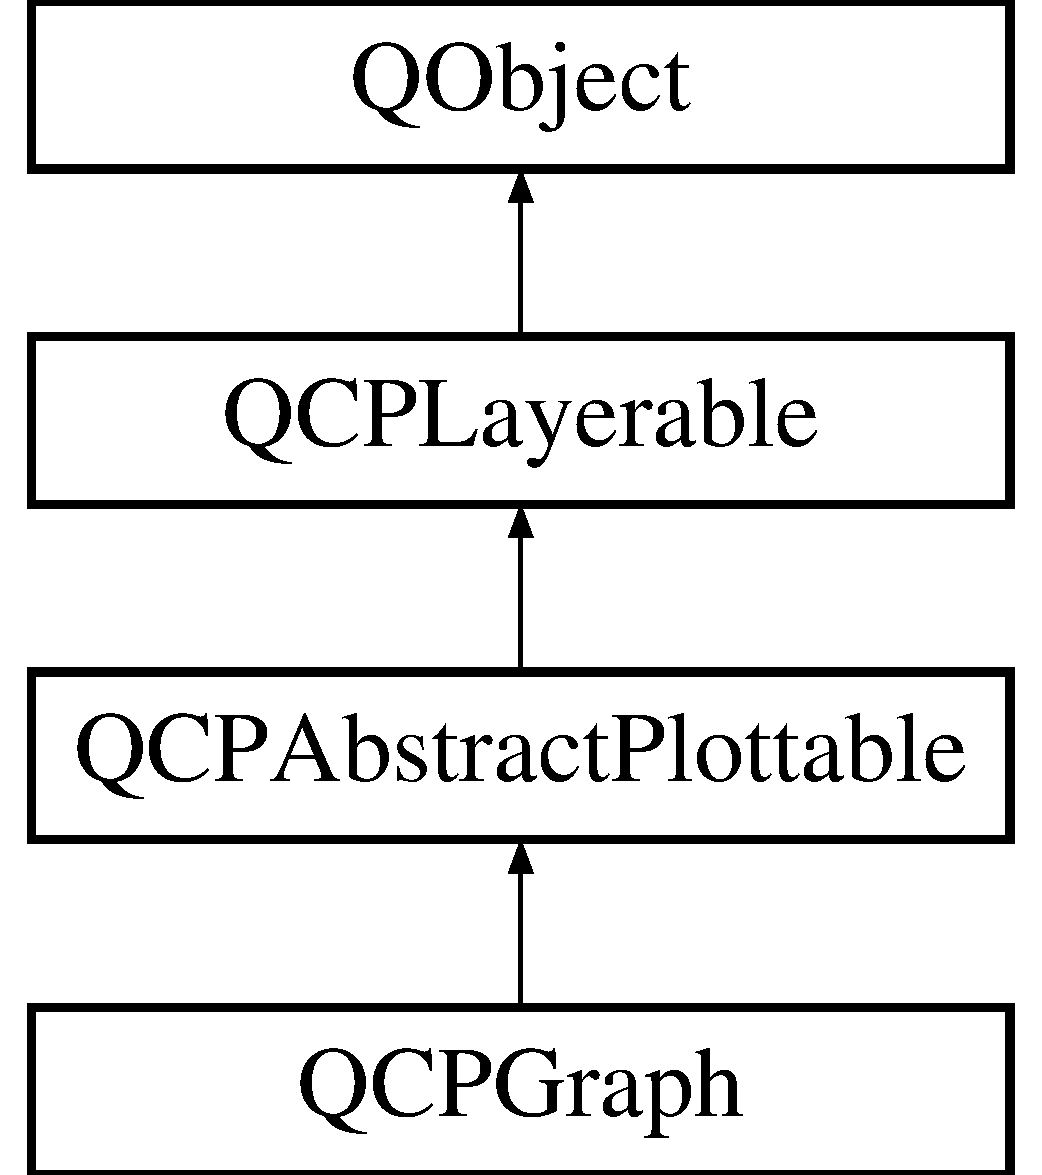
\includegraphics[height=4.000000cm]{class_q_c_p_graph}
\end{center}
\end{figure}
\subsection*{Public Types}
\begin{DoxyCompactItemize}
\item 
enum \hyperlink{class_q_c_p_graph_ad60175cd9b5cac937c5ee685c32c0859}{Line\+Style} \{ \newline
\hyperlink{class_q_c_p_graph_ad60175cd9b5cac937c5ee685c32c0859aea9591b933733cc7b20786b71e60fa04}{ls\+None}, 
\hyperlink{class_q_c_p_graph_ad60175cd9b5cac937c5ee685c32c0859a3c42a27b15aa3c92d399082fad8b7515}{ls\+Line}, 
\hyperlink{class_q_c_p_graph_ad60175cd9b5cac937c5ee685c32c0859ae10568bda57836487d9dec5eba1d6c6e}{ls\+Step\+Left}, 
\hyperlink{class_q_c_p_graph_ad60175cd9b5cac937c5ee685c32c0859a9c37951f7d11aa070100fd16f2935c9e}{ls\+Step\+Right}, 
\newline
\hyperlink{class_q_c_p_graph_ad60175cd9b5cac937c5ee685c32c0859a5adf7b04da215a40a764c21294ea7366}{ls\+Step\+Center}, 
\hyperlink{class_q_c_p_graph_ad60175cd9b5cac937c5ee685c32c0859aa3b358b4ae7cca94aceeb8e529c12ebb}{ls\+Impulse}
 \}
\item 
enum \hyperlink{class_q_c_p_graph_ad23b514404bd2cb3216f57c90904d6af}{Error\+Type} \{ \hyperlink{class_q_c_p_graph_ad23b514404bd2cb3216f57c90904d6afaeae745e7cc1766bb8546e35d4b76a711}{et\+None}, 
\hyperlink{class_q_c_p_graph_ad23b514404bd2cb3216f57c90904d6afa2a5d89cd76fb8b6b18d71b8f6f6c0f43}{et\+Key}, 
\hyperlink{class_q_c_p_graph_ad23b514404bd2cb3216f57c90904d6afa147022ccdc49f6bd48f904cb4f61872e}{et\+Value}, 
\hyperlink{class_q_c_p_graph_ad23b514404bd2cb3216f57c90904d6afa761cb7d61670c1e2efecccd8974409ab}{et\+Both}
 \}
\end{DoxyCompactItemize}
\subsection*{Public Member Functions}
\begin{DoxyCompactItemize}
\item 
\hyperlink{class_q_c_p_graph_a0393a38cf7183cbf46348eb6cf9a5a6c}{Q\+C\+P\+Graph} (\hyperlink{class_q_c_p_axis}{Q\+C\+P\+Axis} $\ast$key\+Axis, \hyperlink{class_q_c_p_axis}{Q\+C\+P\+Axis} $\ast$value\+Axis)
\item 
\hyperlink{qcustomplot_8h_a84a9c4a4c2216ccfdcb5f3067cda76e3}{Q\+C\+P\+Data\+Map} $\ast$ \hyperlink{class_q_c_p_graph_acde1c0d1f6a817930489548396e6b3e6}{data} () const
\item 
\hypertarget{class_q_c_p_graph_ac3e6f4b3387338df45992b47691b2551}{}\label{class_q_c_p_graph_ac3e6f4b3387338df45992b47691b2551} 
\hyperlink{class_q_c_p_graph_ad60175cd9b5cac937c5ee685c32c0859}{Line\+Style} {\bfseries line\+Style} () const
\item 
\hypertarget{class_q_c_p_graph_a36d5b641db08e27527827c212542bbbd}{}\label{class_q_c_p_graph_a36d5b641db08e27527827c212542bbbd} 
\hyperlink{class_q_c_p_scatter_style}{Q\+C\+P\+Scatter\+Style} {\bfseries scatter\+Style} () const
\item 
\hypertarget{class_q_c_p_graph_a1efa62c4b826f34716b505b15d2b2583}{}\label{class_q_c_p_graph_a1efa62c4b826f34716b505b15d2b2583} 
\hyperlink{class_q_c_p_graph_ad23b514404bd2cb3216f57c90904d6af}{Error\+Type} {\bfseries error\+Type} () const
\item 
\hypertarget{class_q_c_p_graph_abcf453d2c0d7a751d3a311a8b919b8d9}{}\label{class_q_c_p_graph_abcf453d2c0d7a751d3a311a8b919b8d9} 
Q\+Pen {\bfseries error\+Pen} () const
\item 
\hypertarget{class_q_c_p_graph_a5b071344b150359aadb7be0b10b0eae9}{}\label{class_q_c_p_graph_a5b071344b150359aadb7be0b10b0eae9} 
double {\bfseries error\+Bar\+Size} () const
\item 
\hypertarget{class_q_c_p_graph_a810db049eff26150c0bcead1bfbcf931}{}\label{class_q_c_p_graph_a810db049eff26150c0bcead1bfbcf931} 
bool {\bfseries error\+Bar\+Skip\+Symbol} () const
\item 
\hypertarget{class_q_c_p_graph_a84277b1655474453a5c83318053414d5}{}\label{class_q_c_p_graph_a84277b1655474453a5c83318053414d5} 
\hyperlink{class_q_c_p_graph}{Q\+C\+P\+Graph} $\ast$ {\bfseries channel\+Fill\+Graph} () const
\item 
\hypertarget{class_q_c_p_graph_a1ba934b9621270b9a40fcdd2d9ba2adb}{}\label{class_q_c_p_graph_a1ba934b9621270b9a40fcdd2d9ba2adb} 
bool {\bfseries adaptive\+Sampling} () const
\item 
void \hyperlink{class_q_c_p_graph_a1df2fd710545c8ba3b2c99a39a27bf8b}{set\+Data} (\hyperlink{qcustomplot_8h_a84a9c4a4c2216ccfdcb5f3067cda76e3}{Q\+C\+P\+Data\+Map} $\ast$\hyperlink{class_q_c_p_graph_acde1c0d1f6a817930489548396e6b3e6}{data}, bool copy=false)
\item 
void \hyperlink{class_q_c_p_graph_a4c55d8ac13bfa42c8c93747820891a76}{set\+Data} (const Q\+Vector$<$ double $>$ \&key, const Q\+Vector$<$ double $>$ \&value)
\item 
void \hyperlink{class_q_c_p_graph_abce9f07c0d722bc3e4fa7bd73c7e5dfa}{set\+Data\+Key\+Error} (const Q\+Vector$<$ double $>$ \&key, const Q\+Vector$<$ double $>$ \&value, const Q\+Vector$<$ double $>$ \&key\+Error)
\item 
void \hyperlink{class_q_c_p_graph_ac15c749c5fedf740d5692c6fe67143b8}{set\+Data\+Key\+Error} (const Q\+Vector$<$ double $>$ \&key, const Q\+Vector$<$ double $>$ \&value, const Q\+Vector$<$ double $>$ \&key\+Error\+Minus, const Q\+Vector$<$ double $>$ \&key\+Error\+Plus)
\item 
void \hyperlink{class_q_c_p_graph_acba6296eadcb36b93267628b8dae3de5}{set\+Data\+Value\+Error} (const Q\+Vector$<$ double $>$ \&key, const Q\+Vector$<$ double $>$ \&value, const Q\+Vector$<$ double $>$ \&value\+Error)
\item 
void \hyperlink{class_q_c_p_graph_a3afbfd7222d739351c69387904776f93}{set\+Data\+Value\+Error} (const Q\+Vector$<$ double $>$ \&key, const Q\+Vector$<$ double $>$ \&value, const Q\+Vector$<$ double $>$ \&value\+Error\+Minus, const Q\+Vector$<$ double $>$ \&value\+Error\+Plus)
\item 
void \hyperlink{class_q_c_p_graph_a873fe46bdb20be5710428e474ade8908}{set\+Data\+Both\+Error} (const Q\+Vector$<$ double $>$ \&key, const Q\+Vector$<$ double $>$ \&value, const Q\+Vector$<$ double $>$ \&key\+Error, const Q\+Vector$<$ double $>$ \&value\+Error)
\item 
void \hyperlink{class_q_c_p_graph_abb75736ecdbf6e6a7501e1da64fb18cf}{set\+Data\+Both\+Error} (const Q\+Vector$<$ double $>$ \&key, const Q\+Vector$<$ double $>$ \&value, const Q\+Vector$<$ double $>$ \&key\+Error\+Minus, const Q\+Vector$<$ double $>$ \&key\+Error\+Plus, const Q\+Vector$<$ double $>$ \&value\+Error\+Minus, const Q\+Vector$<$ double $>$ \&value\+Error\+Plus)
\item 
void \hyperlink{class_q_c_p_graph_a513fecccff5b2a50ce53f665338c60ff}{set\+Line\+Style} (\hyperlink{class_q_c_p_graph_ad60175cd9b5cac937c5ee685c32c0859}{Line\+Style} ls)
\item 
void \hyperlink{class_q_c_p_graph_a12bd17a8ba21983163ec5d8f42a9fea5}{set\+Scatter\+Style} (const \hyperlink{class_q_c_p_scatter_style}{Q\+C\+P\+Scatter\+Style} \&style)
\item 
void \hyperlink{class_q_c_p_graph_ac3614d799c3894f2bc646e99c7f73d38}{set\+Error\+Type} (\hyperlink{class_q_c_p_graph_ad23b514404bd2cb3216f57c90904d6af}{Error\+Type} error\+Type)
\item 
void \hyperlink{class_q_c_p_graph_abd4c7f81939e10776ea64603a704f22a}{set\+Error\+Pen} (const Q\+Pen \&pen)
\item 
void \hyperlink{class_q_c_p_graph_a10f50c5495ce45ef559ec2066194a335}{set\+Error\+Bar\+Size} (double size)
\item 
void \hyperlink{class_q_c_p_graph_ab1c1ee03d8dd94676a564e5e5f11aac2}{set\+Error\+Bar\+Skip\+Symbol} (bool enabled)
\item 
void \hyperlink{class_q_c_p_graph_a2d03156df1b64037a2e36cfa50351ca3}{set\+Channel\+Fill\+Graph} (\hyperlink{class_q_c_p_graph}{Q\+C\+P\+Graph} $\ast$target\+Graph)
\item 
void \hyperlink{class_q_c_p_graph_ab468cd600160f327836aa0644291e64c}{set\+Adaptive\+Sampling} (bool enabled)
\item 
void \hyperlink{class_q_c_p_graph_aa5c6181d84db72ce4dbe9dc15a34ef4f}{add\+Data} (const \hyperlink{qcustomplot_8h_a84a9c4a4c2216ccfdcb5f3067cda76e3}{Q\+C\+P\+Data\+Map} \&data\+Map)
\item 
void \hyperlink{class_q_c_p_graph_a80cc91e1e0ef77eb50afc5b366d0efd9}{add\+Data} (const \hyperlink{class_q_c_p_data}{Q\+C\+P\+Data} \&\hyperlink{class_q_c_p_graph_acde1c0d1f6a817930489548396e6b3e6}{data})
\item 
void \hyperlink{class_q_c_p_graph_a0bf98b1972286cfb7b1c4b7dd6ae2012}{add\+Data} (double key, double value)
\item 
void \hyperlink{class_q_c_p_graph_ab6da6377541fe80d892a9893a92db9c6}{add\+Data} (const Q\+Vector$<$ double $>$ \&keys, const Q\+Vector$<$ double $>$ \&values)
\item 
void \hyperlink{class_q_c_p_graph_a9fe0b3e54e8c7b61319bd03337e21e99}{remove\+Data\+Before} (double key)
\item 
void \hyperlink{class_q_c_p_graph_ae42d645ef617cfc75fc0df58e62c522a}{remove\+Data\+After} (double key)
\item 
void \hyperlink{class_q_c_p_graph_a4a0fde50b7db9db0a85b5c5b6b10098f}{remove\+Data} (double from\+Key, double to\+Key)
\item 
void \hyperlink{class_q_c_p_graph_a4a706020b4318f118381648ef18aca3f}{remove\+Data} (double key)
\item 
virtual void \hyperlink{class_q_c_p_graph_ad4e94a4e44e5e76fbec81a72a977157d}{clear\+Data} ()
\item 
virtual double \hyperlink{class_q_c_p_graph_a36011c34aca4f7a477de25961e2f6c13}{select\+Test} (const Q\+PointF \&pos, bool only\+Selectable, Q\+Variant $\ast$details=0) const
\item 
void \hyperlink{class_q_c_p_graph_a9c3909d6116e9d03978f057d41174e6a}{rescale\+Axes} (bool only\+Enlarge, bool include\+Error\+Bars) const
\item 
void \hyperlink{class_q_c_p_graph_a051fb77b459ba1ae8d65552c67f45e94}{rescale\+Key\+Axis} (bool only\+Enlarge, bool include\+Error\+Bars) const
\item 
void \hyperlink{class_q_c_p_graph_a9e0e620a56932c4df80a3762c2f93608}{rescale\+Value\+Axis} (bool only\+Enlarge, bool include\+Error\+Bars) const
\end{DoxyCompactItemize}
\subsection*{Protected Member Functions}
\begin{DoxyCompactItemize}
\item 
\hypertarget{class_q_c_p_graph_a659218cc62c2a7786213d9dd429c1c8d}{}\label{class_q_c_p_graph_a659218cc62c2a7786213d9dd429c1c8d} 
virtual void {\bfseries draw} (\hyperlink{class_q_c_p_painter}{Q\+C\+P\+Painter} $\ast$painter)
\item 
\hypertarget{class_q_c_p_graph_ae962caca309faae29ce0988d0d0eff4b}{}\label{class_q_c_p_graph_ae962caca309faae29ce0988d0d0eff4b} 
virtual void {\bfseries draw\+Legend\+Icon} (\hyperlink{class_q_c_p_painter}{Q\+C\+P\+Painter} $\ast$painter, const Q\+RectF \&rect) const
\item 
\hypertarget{class_q_c_p_graph_ad65bc571de3bd0af36296a3cbd0d77ee}{}\label{class_q_c_p_graph_ad65bc571de3bd0af36296a3cbd0d77ee} 
virtual \hyperlink{class_q_c_p_range}{Q\+C\+P\+Range} {\bfseries get\+Key\+Range} (bool \&found\+Range, \hyperlink{class_q_c_p_abstract_plottable_a661743478a1d3c09d28ec2711d7653d8}{Sign\+Domain} in\+Sign\+Domain=\hyperlink{class_q_c_p_abstract_plottable_a661743478a1d3c09d28ec2711d7653d8a082b98cfb91a7363a3b5cd17b0c1cd60}{sd\+Both}) const
\item 
\hypertarget{class_q_c_p_graph_ac205efd80b4a70d67b163429dc6cba8d}{}\label{class_q_c_p_graph_ac205efd80b4a70d67b163429dc6cba8d} 
virtual \hyperlink{class_q_c_p_range}{Q\+C\+P\+Range} {\bfseries get\+Value\+Range} (bool \&found\+Range, \hyperlink{class_q_c_p_abstract_plottable_a661743478a1d3c09d28ec2711d7653d8}{Sign\+Domain} in\+Sign\+Domain=\hyperlink{class_q_c_p_abstract_plottable_a661743478a1d3c09d28ec2711d7653d8a082b98cfb91a7363a3b5cd17b0c1cd60}{sd\+Both}) const
\item 
virtual \hyperlink{class_q_c_p_range}{Q\+C\+P\+Range} \hyperlink{class_q_c_p_graph_ae6425d5df537c08159f794cb18c051c3}{get\+Key\+Range} (bool \&found\+Range, \hyperlink{class_q_c_p_abstract_plottable_a661743478a1d3c09d28ec2711d7653d8}{Sign\+Domain} in\+Sign\+Domain, bool include\+Errors) const
\item 
virtual \hyperlink{class_q_c_p_range}{Q\+C\+P\+Range} \hyperlink{class_q_c_p_graph_ac23c7702ca836c7055f48e6fc3295ca4}{get\+Value\+Range} (bool \&found\+Range, \hyperlink{class_q_c_p_abstract_plottable_a661743478a1d3c09d28ec2711d7653d8}{Sign\+Domain} in\+Sign\+Domain, bool include\+Errors) const
\item 
\hypertarget{class_q_c_p_graph_a9e6ce6db9aa7b29fc397c724fcf7b126}{}\label{class_q_c_p_graph_a9e6ce6db9aa7b29fc397c724fcf7b126} 
virtual void {\bfseries draw\+Fill} (\hyperlink{class_q_c_p_painter}{Q\+C\+P\+Painter} $\ast$painter, Q\+Vector$<$ Q\+PointF $>$ $\ast$line\+Data) const
\item 
\hypertarget{class_q_c_p_graph_ae1f3edd5eb41aa5782e61673488fd3e0}{}\label{class_q_c_p_graph_ae1f3edd5eb41aa5782e61673488fd3e0} 
virtual void {\bfseries draw\+Scatter\+Plot} (\hyperlink{class_q_c_p_painter}{Q\+C\+P\+Painter} $\ast$painter, Q\+Vector$<$ \hyperlink{class_q_c_p_data}{Q\+C\+P\+Data} $>$ $\ast$scatter\+Data) const
\item 
\hypertarget{class_q_c_p_graph_af460db06d4d6466806721fe101f512e3}{}\label{class_q_c_p_graph_af460db06d4d6466806721fe101f512e3} 
virtual void {\bfseries draw\+Line\+Plot} (\hyperlink{class_q_c_p_painter}{Q\+C\+P\+Painter} $\ast$painter, Q\+Vector$<$ Q\+PointF $>$ $\ast$line\+Data) const
\item 
\hypertarget{class_q_c_p_graph_ac62c84f51d85b78ee583455b8c37ba56}{}\label{class_q_c_p_graph_ac62c84f51d85b78ee583455b8c37ba56} 
virtual void {\bfseries draw\+Impulse\+Plot} (\hyperlink{class_q_c_p_painter}{Q\+C\+P\+Painter} $\ast$painter, Q\+Vector$<$ Q\+PointF $>$ $\ast$line\+Data) const
\item 
\hypertarget{class_q_c_p_graph_ae853c297da9d21b6720d2d1c3b0121bf}{}\label{class_q_c_p_graph_ae853c297da9d21b6720d2d1c3b0121bf} 
void {\bfseries get\+Prepared\+Data} (Q\+Vector$<$ \hyperlink{class_q_c_p_data}{Q\+C\+P\+Data} $>$ $\ast$line\+Data, Q\+Vector$<$ \hyperlink{class_q_c_p_data}{Q\+C\+P\+Data} $>$ $\ast$scatter\+Data) const
\item 
\hypertarget{class_q_c_p_graph_a5ec495f97b8185ba9712430cb1558f52}{}\label{class_q_c_p_graph_a5ec495f97b8185ba9712430cb1558f52} 
void {\bfseries get\+Plot\+Data} (Q\+Vector$<$ Q\+PointF $>$ $\ast$line\+Data, Q\+Vector$<$ \hyperlink{class_q_c_p_data}{Q\+C\+P\+Data} $>$ $\ast$scatter\+Data) const
\item 
\hypertarget{class_q_c_p_graph_a6ea929da420e6c104998060d19740ed6}{}\label{class_q_c_p_graph_a6ea929da420e6c104998060d19740ed6} 
void {\bfseries get\+Scatter\+Plot\+Data} (Q\+Vector$<$ \hyperlink{class_q_c_p_data}{Q\+C\+P\+Data} $>$ $\ast$scatter\+Data) const
\item 
\hypertarget{class_q_c_p_graph_a77314984a7af578a66e939db0db48556}{}\label{class_q_c_p_graph_a77314984a7af578a66e939db0db48556} 
void {\bfseries get\+Line\+Plot\+Data} (Q\+Vector$<$ Q\+PointF $>$ $\ast$line\+Pixel\+Data, Q\+Vector$<$ \hyperlink{class_q_c_p_data}{Q\+C\+P\+Data} $>$ $\ast$scatter\+Data) const
\item 
\hypertarget{class_q_c_p_graph_a8f8ae9cb4aa312c2085c3f6f298f19d4}{}\label{class_q_c_p_graph_a8f8ae9cb4aa312c2085c3f6f298f19d4} 
void {\bfseries get\+Step\+Left\+Plot\+Data} (Q\+Vector$<$ Q\+PointF $>$ $\ast$line\+Pixel\+Data, Q\+Vector$<$ \hyperlink{class_q_c_p_data}{Q\+C\+P\+Data} $>$ $\ast$scatter\+Data) const
\item 
\hypertarget{class_q_c_p_graph_a59fecb135f47db10e14d75018210bf80}{}\label{class_q_c_p_graph_a59fecb135f47db10e14d75018210bf80} 
void {\bfseries get\+Step\+Right\+Plot\+Data} (Q\+Vector$<$ Q\+PointF $>$ $\ast$line\+Pixel\+Data, Q\+Vector$<$ \hyperlink{class_q_c_p_data}{Q\+C\+P\+Data} $>$ $\ast$scatter\+Data) const
\item 
\hypertarget{class_q_c_p_graph_ab860d67ecc7e2d7253ab1f19032958c2}{}\label{class_q_c_p_graph_ab860d67ecc7e2d7253ab1f19032958c2} 
void {\bfseries get\+Step\+Center\+Plot\+Data} (Q\+Vector$<$ Q\+PointF $>$ $\ast$line\+Pixel\+Data, Q\+Vector$<$ \hyperlink{class_q_c_p_data}{Q\+C\+P\+Data} $>$ $\ast$scatter\+Data) const
\item 
\hypertarget{class_q_c_p_graph_aae73c001a78cbe54e55e6779d7a70957}{}\label{class_q_c_p_graph_aae73c001a78cbe54e55e6779d7a70957} 
void {\bfseries get\+Impulse\+Plot\+Data} (Q\+Vector$<$ Q\+PointF $>$ $\ast$line\+Pixel\+Data, Q\+Vector$<$ \hyperlink{class_q_c_p_data}{Q\+C\+P\+Data} $>$ $\ast$scatter\+Data) const
\item 
\hypertarget{class_q_c_p_graph_ab51aeba7e9d29754e58852cfad3436cc}{}\label{class_q_c_p_graph_ab51aeba7e9d29754e58852cfad3436cc} 
void {\bfseries draw\+Error} (\hyperlink{class_q_c_p_painter}{Q\+C\+P\+Painter} $\ast$painter, double x, double y, const \hyperlink{class_q_c_p_data}{Q\+C\+P\+Data} \&\hyperlink{class_q_c_p_graph_acde1c0d1f6a817930489548396e6b3e6}{data}) const
\item 
\hypertarget{class_q_c_p_graph_abda485a2f71ebe00d890840acbb91516}{}\label{class_q_c_p_graph_abda485a2f71ebe00d890840acbb91516} 
void {\bfseries get\+Visible\+Data\+Bounds} (Q\+C\+P\+Data\+Map\+::const\+\_\+iterator \&lower, Q\+C\+P\+Data\+Map\+::const\+\_\+iterator \&upper) const
\item 
\hypertarget{class_q_c_p_graph_ae413e4ea50fea821a48ee2b3c4aaa055}{}\label{class_q_c_p_graph_ae413e4ea50fea821a48ee2b3c4aaa055} 
int {\bfseries count\+Data\+In\+Bounds} (const Q\+C\+P\+Data\+Map\+::const\+\_\+iterator \&lower, const Q\+C\+P\+Data\+Map\+::const\+\_\+iterator \&upper, int max\+Count) const
\item 
\hypertarget{class_q_c_p_graph_a8e517dcd3baba1b41daed0248841c092}{}\label{class_q_c_p_graph_a8e517dcd3baba1b41daed0248841c092} 
void {\bfseries add\+Fill\+Base\+Points} (Q\+Vector$<$ Q\+PointF $>$ $\ast$line\+Data) const
\item 
\hypertarget{class_q_c_p_graph_aff2ae149f6d319fc3ed2c7c6fb348553}{}\label{class_q_c_p_graph_aff2ae149f6d319fc3ed2c7c6fb348553} 
void {\bfseries remove\+Fill\+Base\+Points} (Q\+Vector$<$ Q\+PointF $>$ $\ast$line\+Data) const
\item 
\hypertarget{class_q_c_p_graph_ace7c17a07e9aa824853e469816a5aa1c}{}\label{class_q_c_p_graph_ace7c17a07e9aa824853e469816a5aa1c} 
Q\+PointF {\bfseries lower\+Fill\+Base\+Point} (double lower\+Key) const
\item 
\hypertarget{class_q_c_p_graph_a7a255fc7260d96ed6f9d972839941f93}{}\label{class_q_c_p_graph_a7a255fc7260d96ed6f9d972839941f93} 
Q\+PointF {\bfseries upper\+Fill\+Base\+Point} (double upper\+Key) const
\item 
\hypertarget{class_q_c_p_graph_add26655bd2338adaa7fc99e27bd06550}{}\label{class_q_c_p_graph_add26655bd2338adaa7fc99e27bd06550} 
const Q\+PolygonF {\bfseries get\+Channel\+Fill\+Polygon} (const Q\+Vector$<$ Q\+PointF $>$ $\ast$line\+Data) const
\item 
\hypertarget{class_q_c_p_graph_a8c3f15dd5a06633011a6ef36016d308b}{}\label{class_q_c_p_graph_a8c3f15dd5a06633011a6ef36016d308b} 
int {\bfseries find\+Index\+BelowX} (const Q\+Vector$<$ Q\+PointF $>$ $\ast$\hyperlink{class_q_c_p_graph_acde1c0d1f6a817930489548396e6b3e6}{data}, double x) const
\item 
\hypertarget{class_q_c_p_graph_aaabd6c6a7200a2672c44e62bd2a1cafa}{}\label{class_q_c_p_graph_aaabd6c6a7200a2672c44e62bd2a1cafa} 
int {\bfseries find\+Index\+AboveX} (const Q\+Vector$<$ Q\+PointF $>$ $\ast$\hyperlink{class_q_c_p_graph_acde1c0d1f6a817930489548396e6b3e6}{data}, double x) const
\item 
\hypertarget{class_q_c_p_graph_a5b0291f248e8ca8eaa82833ab420dcd0}{}\label{class_q_c_p_graph_a5b0291f248e8ca8eaa82833ab420dcd0} 
int {\bfseries find\+Index\+BelowY} (const Q\+Vector$<$ Q\+PointF $>$ $\ast$\hyperlink{class_q_c_p_graph_acde1c0d1f6a817930489548396e6b3e6}{data}, double y) const
\item 
\hypertarget{class_q_c_p_graph_a8b952a5f937840dc242489585cc8000d}{}\label{class_q_c_p_graph_a8b952a5f937840dc242489585cc8000d} 
int {\bfseries find\+Index\+AboveY} (const Q\+Vector$<$ Q\+PointF $>$ $\ast$\hyperlink{class_q_c_p_graph_acde1c0d1f6a817930489548396e6b3e6}{data}, double y) const
\item 
\hypertarget{class_q_c_p_graph_a96146099a5e68f49c7326a765f768da2}{}\label{class_q_c_p_graph_a96146099a5e68f49c7326a765f768da2} 
double {\bfseries point\+Distance} (const Q\+PointF \&pixel\+Point) const
\end{DoxyCompactItemize}
\subsection*{Protected Attributes}
\begin{DoxyCompactItemize}
\item 
\hypertarget{class_q_c_p_graph_a8457c840f69a0ac49f61d30a509c5d08}{}\label{class_q_c_p_graph_a8457c840f69a0ac49f61d30a509c5d08} 
\hyperlink{qcustomplot_8h_a84a9c4a4c2216ccfdcb5f3067cda76e3}{Q\+C\+P\+Data\+Map} $\ast$ {\bfseries m\+Data}
\item 
\hypertarget{class_q_c_p_graph_aa35681a24165c2831301091a87b662ce}{}\label{class_q_c_p_graph_aa35681a24165c2831301091a87b662ce} 
Q\+Pen {\bfseries m\+Error\+Pen}
\item 
\hypertarget{class_q_c_p_graph_a8604fd98402035a63375849f7341ee25}{}\label{class_q_c_p_graph_a8604fd98402035a63375849f7341ee25} 
\hyperlink{class_q_c_p_graph_ad60175cd9b5cac937c5ee685c32c0859}{Line\+Style} {\bfseries m\+Line\+Style}
\item 
\hypertarget{class_q_c_p_graph_a4aa36241f166ccd1f75fc8f24e4a3247}{}\label{class_q_c_p_graph_a4aa36241f166ccd1f75fc8f24e4a3247} 
\hyperlink{class_q_c_p_scatter_style}{Q\+C\+P\+Scatter\+Style} {\bfseries m\+Scatter\+Style}
\item 
\hypertarget{class_q_c_p_graph_a29e64273db201aeadebc61c870720a36}{}\label{class_q_c_p_graph_a29e64273db201aeadebc61c870720a36} 
\hyperlink{class_q_c_p_graph_ad23b514404bd2cb3216f57c90904d6af}{Error\+Type} {\bfseries m\+Error\+Type}
\item 
\hypertarget{class_q_c_p_graph_a7b51c8d09510f9d195b5e765ccbcf05b}{}\label{class_q_c_p_graph_a7b51c8d09510f9d195b5e765ccbcf05b} 
double {\bfseries m\+Error\+Bar\+Size}
\item 
\hypertarget{class_q_c_p_graph_acf631d7dbd1055a69ab3b63094868557}{}\label{class_q_c_p_graph_acf631d7dbd1055a69ab3b63094868557} 
bool {\bfseries m\+Error\+Bar\+Skip\+Symbol}
\item 
\hypertarget{class_q_c_p_graph_a2f1777c7accf8244fc640c33f0b04577}{}\label{class_q_c_p_graph_a2f1777c7accf8244fc640c33f0b04577} 
Q\+Pointer$<$ \hyperlink{class_q_c_p_graph}{Q\+C\+P\+Graph} $>$ {\bfseries m\+Channel\+Fill\+Graph}
\item 
\hypertarget{class_q_c_p_graph_aa951e78aeba714cf443be6da2e52502e}{}\label{class_q_c_p_graph_aa951e78aeba714cf443be6da2e52502e} 
bool {\bfseries m\+Adaptive\+Sampling}
\end{DoxyCompactItemize}
\subsection*{Friends}
\begin{DoxyCompactItemize}
\item 
\hypertarget{class_q_c_p_graph_a1cdf9df76adcfae45261690aa0ca2198}{}\label{class_q_c_p_graph_a1cdf9df76adcfae45261690aa0ca2198} 
class {\bfseries Q\+Custom\+Plot}
\item 
\hypertarget{class_q_c_p_graph_a8429035e7adfbd7f05805a6530ad5e3b}{}\label{class_q_c_p_graph_a8429035e7adfbd7f05805a6530ad5e3b} 
class {\bfseries Q\+C\+P\+Legend}
\end{DoxyCompactItemize}
\subsection*{Additional Inherited Members}


\subsection{Detailed Description}
A plottable representing a graph in a plot. 



Usually you create new graphs by calling \hyperlink{class_q_custom_plot_a6fb2873d35a8a8089842d81a70a54167}{Q\+Custom\+Plot\+::add\+Graph}. The resulting instance can be accessed via \hyperlink{class_q_custom_plot_a6ecae130f684b25276fb47bd3a5875c6}{Q\+Custom\+Plot\+::graph}.

To plot data, assign it with the \hyperlink{class_q_c_p_graph_a1df2fd710545c8ba3b2c99a39a27bf8b}{set\+Data} or \hyperlink{class_q_c_p_graph_aa5c6181d84db72ce4dbe9dc15a34ef4f}{add\+Data} functions. Alternatively, you can also access and modify the graph\textquotesingle{}s data via the \hyperlink{class_q_c_p_graph_acde1c0d1f6a817930489548396e6b3e6}{data} method, which returns a pointer to the internal \hyperlink{qcustomplot_8h_a84a9c4a4c2216ccfdcb5f3067cda76e3}{Q\+C\+P\+Data\+Map}.

Graphs are used to display single-\/valued data. Single-\/valued means that there should only be one data point per unique key coordinate. In other words, the graph can\textquotesingle{}t have {\itshape loops}. If you do want to plot non-\/single-\/valued curves, rather use the \hyperlink{class_q_c_p_curve}{Q\+C\+P\+Curve} plottable.

Gaps in the graph line can be created by adding data points with NaN as value ({\ttfamily q\+Q\+Na\+N()} or {\ttfamily std\+::numeric\+\_\+limits$<$double$>$\+::quiet\+\_\+\+Na\+N()}) in between the two data points that shall be separated.\hypertarget{class_q_c_p_statistical_box_appearance}{}\subsection{Changing the appearance}\label{class_q_c_p_statistical_box_appearance}
The appearance of the graph is mainly determined by the line style, scatter style, brush and pen of the graph (\hyperlink{class_q_c_p_graph_a513fecccff5b2a50ce53f665338c60ff}{set\+Line\+Style}, \hyperlink{class_q_c_p_graph_a12bd17a8ba21983163ec5d8f42a9fea5}{set\+Scatter\+Style}, \hyperlink{class_q_c_p_abstract_plottable_a7a4b92144dca6453a1f0f210e27edc74}{set\+Brush}, \hyperlink{class_q_c_p_abstract_plottable_ab74b09ae4c0e7e13142fe4b5bf46cac7}{set\+Pen}).\hypertarget{class_q_c_p_graph_filling}{}\subsubsection{Filling under or between graphs}\label{class_q_c_p_graph_filling}
\hyperlink{class_q_c_p_graph}{Q\+C\+P\+Graph} knows two types of fills\+: Normal graph fills towards the zero-\/value-\/line parallel to the key axis of the graph, and fills between two graphs, called channel fills. To enable a fill, just set a brush with \hyperlink{class_q_c_p_abstract_plottable_a7a4b92144dca6453a1f0f210e27edc74}{set\+Brush} which is neither Qt\+::\+No\+Brush nor fully transparent.

By default, a normal fill towards the zero-\/value-\/line will be drawn. To set up a channel fill between this graph and another one, call \hyperlink{class_q_c_p_graph_a2d03156df1b64037a2e36cfa50351ca3}{set\+Channel\+Fill\+Graph} with the other graph as parameter.

\begin{DoxySeeAlso}{See also}
\hyperlink{class_q_custom_plot_a6fb2873d35a8a8089842d81a70a54167}{Q\+Custom\+Plot\+::add\+Graph}, \hyperlink{class_q_custom_plot_a6ecae130f684b25276fb47bd3a5875c6}{Q\+Custom\+Plot\+::graph} 
\end{DoxySeeAlso}


\subsection{Member Enumeration Documentation}
\hypertarget{class_q_c_p_graph_ad23b514404bd2cb3216f57c90904d6af}{}\label{class_q_c_p_graph_ad23b514404bd2cb3216f57c90904d6af} 
\index{Q\+C\+P\+Graph@{Q\+C\+P\+Graph}!Error\+Type@{Error\+Type}}
\index{Error\+Type@{Error\+Type}!Q\+C\+P\+Graph@{Q\+C\+P\+Graph}}
\subsubsection{\texorpdfstring{Error\+Type}{ErrorType}}
{\footnotesize\ttfamily enum \hyperlink{class_q_c_p_graph_ad23b514404bd2cb3216f57c90904d6af}{Q\+C\+P\+Graph\+::\+Error\+Type}}

Defines what kind of error bars are drawn for each data point \begin{DoxyEnumFields}{Enumerator}
\raisebox{\heightof{T}}[0pt][0pt]{\index{et\+None@{et\+None}!Q\+C\+P\+Graph@{Q\+C\+P\+Graph}}\index{Q\+C\+P\+Graph@{Q\+C\+P\+Graph}!et\+None@{et\+None}}}\hypertarget{class_q_c_p_graph_ad23b514404bd2cb3216f57c90904d6afaeae745e7cc1766bb8546e35d4b76a711}{}\label{class_q_c_p_graph_ad23b514404bd2cb3216f57c90904d6afaeae745e7cc1766bb8546e35d4b76a711} 
et\+None&No error bars are shown. \\
\hline

\raisebox{\heightof{T}}[0pt][0pt]{\index{et\+Key@{et\+Key}!Q\+C\+P\+Graph@{Q\+C\+P\+Graph}}\index{Q\+C\+P\+Graph@{Q\+C\+P\+Graph}!et\+Key@{et\+Key}}}\hypertarget{class_q_c_p_graph_ad23b514404bd2cb3216f57c90904d6afa2a5d89cd76fb8b6b18d71b8f6f6c0f43}{}\label{class_q_c_p_graph_ad23b514404bd2cb3216f57c90904d6afa2a5d89cd76fb8b6b18d71b8f6f6c0f43} 
et\+Key&Error bars for the key dimension of the data point are shown. \\
\hline

\raisebox{\heightof{T}}[0pt][0pt]{\index{et\+Value@{et\+Value}!Q\+C\+P\+Graph@{Q\+C\+P\+Graph}}\index{Q\+C\+P\+Graph@{Q\+C\+P\+Graph}!et\+Value@{et\+Value}}}\hypertarget{class_q_c_p_graph_ad23b514404bd2cb3216f57c90904d6afa147022ccdc49f6bd48f904cb4f61872e}{}\label{class_q_c_p_graph_ad23b514404bd2cb3216f57c90904d6afa147022ccdc49f6bd48f904cb4f61872e} 
et\+Value&Error bars for the value dimension of the data point are shown. \\
\hline

\raisebox{\heightof{T}}[0pt][0pt]{\index{et\+Both@{et\+Both}!Q\+C\+P\+Graph@{Q\+C\+P\+Graph}}\index{Q\+C\+P\+Graph@{Q\+C\+P\+Graph}!et\+Both@{et\+Both}}}\hypertarget{class_q_c_p_graph_ad23b514404bd2cb3216f57c90904d6afa761cb7d61670c1e2efecccd8974409ab}{}\label{class_q_c_p_graph_ad23b514404bd2cb3216f57c90904d6afa761cb7d61670c1e2efecccd8974409ab} 
et\+Both&Error bars for both key and value dimensions of the data point are shown. \\
\hline

\end{DoxyEnumFields}
\hypertarget{class_q_c_p_graph_ad60175cd9b5cac937c5ee685c32c0859}{}\label{class_q_c_p_graph_ad60175cd9b5cac937c5ee685c32c0859} 
\index{Q\+C\+P\+Graph@{Q\+C\+P\+Graph}!Line\+Style@{Line\+Style}}
\index{Line\+Style@{Line\+Style}!Q\+C\+P\+Graph@{Q\+C\+P\+Graph}}
\subsubsection{\texorpdfstring{Line\+Style}{LineStyle}}
{\footnotesize\ttfamily enum \hyperlink{class_q_c_p_graph_ad60175cd9b5cac937c5ee685c32c0859}{Q\+C\+P\+Graph\+::\+Line\+Style}}

Defines how the graph\textquotesingle{}s line is represented visually in the plot. The line is drawn with the current pen of the graph (\hyperlink{class_q_c_p_abstract_plottable_ab74b09ae4c0e7e13142fe4b5bf46cac7}{set\+Pen}). \begin{DoxySeeAlso}{See also}
\hyperlink{class_q_c_p_graph_a513fecccff5b2a50ce53f665338c60ff}{set\+Line\+Style} 
\end{DoxySeeAlso}
\begin{DoxyEnumFields}{Enumerator}
\raisebox{\heightof{T}}[0pt][0pt]{\index{ls\+None@{ls\+None}!Q\+C\+P\+Graph@{Q\+C\+P\+Graph}}\index{Q\+C\+P\+Graph@{Q\+C\+P\+Graph}!ls\+None@{ls\+None}}}\hypertarget{class_q_c_p_graph_ad60175cd9b5cac937c5ee685c32c0859aea9591b933733cc7b20786b71e60fa04}{}\label{class_q_c_p_graph_ad60175cd9b5cac937c5ee685c32c0859aea9591b933733cc7b20786b71e60fa04} 
ls\+None&data points are not connected with any lines (e.\+g. data only represented with symbols according to the scatter style, see \hyperlink{class_q_c_p_graph_a12bd17a8ba21983163ec5d8f42a9fea5}{set\+Scatter\+Style}) \\
\hline

\raisebox{\heightof{T}}[0pt][0pt]{\index{ls\+Line@{ls\+Line}!Q\+C\+P\+Graph@{Q\+C\+P\+Graph}}\index{Q\+C\+P\+Graph@{Q\+C\+P\+Graph}!ls\+Line@{ls\+Line}}}\hypertarget{class_q_c_p_graph_ad60175cd9b5cac937c5ee685c32c0859a3c42a27b15aa3c92d399082fad8b7515}{}\label{class_q_c_p_graph_ad60175cd9b5cac937c5ee685c32c0859a3c42a27b15aa3c92d399082fad8b7515} 
ls\+Line&data points are connected by a straight line \\
\hline

\raisebox{\heightof{T}}[0pt][0pt]{\index{ls\+Step\+Left@{ls\+Step\+Left}!Q\+C\+P\+Graph@{Q\+C\+P\+Graph}}\index{Q\+C\+P\+Graph@{Q\+C\+P\+Graph}!ls\+Step\+Left@{ls\+Step\+Left}}}\hypertarget{class_q_c_p_graph_ad60175cd9b5cac937c5ee685c32c0859ae10568bda57836487d9dec5eba1d6c6e}{}\label{class_q_c_p_graph_ad60175cd9b5cac937c5ee685c32c0859ae10568bda57836487d9dec5eba1d6c6e} 
ls\+Step\+Left&line is drawn as steps where the step height is the value of the left data point \\
\hline

\raisebox{\heightof{T}}[0pt][0pt]{\index{ls\+Step\+Right@{ls\+Step\+Right}!Q\+C\+P\+Graph@{Q\+C\+P\+Graph}}\index{Q\+C\+P\+Graph@{Q\+C\+P\+Graph}!ls\+Step\+Right@{ls\+Step\+Right}}}\hypertarget{class_q_c_p_graph_ad60175cd9b5cac937c5ee685c32c0859a9c37951f7d11aa070100fd16f2935c9e}{}\label{class_q_c_p_graph_ad60175cd9b5cac937c5ee685c32c0859a9c37951f7d11aa070100fd16f2935c9e} 
ls\+Step\+Right&line is drawn as steps where the step height is the value of the right data point \\
\hline

\raisebox{\heightof{T}}[0pt][0pt]{\index{ls\+Step\+Center@{ls\+Step\+Center}!Q\+C\+P\+Graph@{Q\+C\+P\+Graph}}\index{Q\+C\+P\+Graph@{Q\+C\+P\+Graph}!ls\+Step\+Center@{ls\+Step\+Center}}}\hypertarget{class_q_c_p_graph_ad60175cd9b5cac937c5ee685c32c0859a5adf7b04da215a40a764c21294ea7366}{}\label{class_q_c_p_graph_ad60175cd9b5cac937c5ee685c32c0859a5adf7b04da215a40a764c21294ea7366} 
ls\+Step\+Center&line is drawn as steps where the step is in between two data points \\
\hline

\raisebox{\heightof{T}}[0pt][0pt]{\index{ls\+Impulse@{ls\+Impulse}!Q\+C\+P\+Graph@{Q\+C\+P\+Graph}}\index{Q\+C\+P\+Graph@{Q\+C\+P\+Graph}!ls\+Impulse@{ls\+Impulse}}}\hypertarget{class_q_c_p_graph_ad60175cd9b5cac937c5ee685c32c0859aa3b358b4ae7cca94aceeb8e529c12ebb}{}\label{class_q_c_p_graph_ad60175cd9b5cac937c5ee685c32c0859aa3b358b4ae7cca94aceeb8e529c12ebb} 
ls\+Impulse&each data point is represented by a line parallel to the value axis, which reaches from the data point to the zero-\/value-\/line \\
\hline

\end{DoxyEnumFields}


\subsection{Constructor \& Destructor Documentation}
\hypertarget{class_q_c_p_graph_a0393a38cf7183cbf46348eb6cf9a5a6c}{}\label{class_q_c_p_graph_a0393a38cf7183cbf46348eb6cf9a5a6c} 
\index{Q\+C\+P\+Graph@{Q\+C\+P\+Graph}!Q\+C\+P\+Graph@{Q\+C\+P\+Graph}}
\index{Q\+C\+P\+Graph@{Q\+C\+P\+Graph}!Q\+C\+P\+Graph@{Q\+C\+P\+Graph}}
\subsubsection{\texorpdfstring{Q\+C\+P\+Graph()}{QCPGraph()}}
{\footnotesize\ttfamily Q\+C\+P\+Graph\+::\+Q\+C\+P\+Graph (\begin{DoxyParamCaption}\item[{\hyperlink{class_q_c_p_axis}{Q\+C\+P\+Axis} $\ast$}]{key\+Axis,  }\item[{\hyperlink{class_q_c_p_axis}{Q\+C\+P\+Axis} $\ast$}]{value\+Axis }\end{DoxyParamCaption})\hspace{0.3cm}{\ttfamily [explicit]}}

Constructs a graph which uses {\itshape key\+Axis} as its key axis (\char`\"{}x\char`\"{}) and {\itshape value\+Axis} as its value axis (\char`\"{}y\char`\"{}). {\itshape key\+Axis} and {\itshape value\+Axis} must reside in the same \hyperlink{class_q_custom_plot}{Q\+Custom\+Plot} instance and not have the same orientation. If either of these restrictions is violated, a corresponding message is printed to the debug output (q\+Debug), the construction is not aborted, though.

The constructed \hyperlink{class_q_c_p_graph}{Q\+C\+P\+Graph} can be added to the plot with \hyperlink{class_q_custom_plot_ab7ad9174f701f9c6f64e378df77927a6}{Q\+Custom\+Plot\+::add\+Plottable}, \hyperlink{class_q_custom_plot}{Q\+Custom\+Plot} then takes ownership of the graph.

To directly create a graph inside a plot, you can also use the simpler \hyperlink{class_q_custom_plot_a6fb2873d35a8a8089842d81a70a54167}{Q\+Custom\+Plot\+::add\+Graph} function. 

\subsection{Member Function Documentation}
\hypertarget{class_q_c_p_graph_aa5c6181d84db72ce4dbe9dc15a34ef4f}{}\label{class_q_c_p_graph_aa5c6181d84db72ce4dbe9dc15a34ef4f} 
\index{Q\+C\+P\+Graph@{Q\+C\+P\+Graph}!add\+Data@{add\+Data}}
\index{add\+Data@{add\+Data}!Q\+C\+P\+Graph@{Q\+C\+P\+Graph}}
\subsubsection{\texorpdfstring{add\+Data()}{addData()}\hspace{0.1cm}{\footnotesize\ttfamily [1/4]}}
{\footnotesize\ttfamily void Q\+C\+P\+Graph\+::add\+Data (\begin{DoxyParamCaption}\item[{const \hyperlink{qcustomplot_8h_a84a9c4a4c2216ccfdcb5f3067cda76e3}{Q\+C\+P\+Data\+Map} \&}]{data\+Map }\end{DoxyParamCaption})}

Adds the provided data points in {\itshape data\+Map} to the current data.

Alternatively, you can also access and modify the graph\textquotesingle{}s data via the \hyperlink{class_q_c_p_graph_acde1c0d1f6a817930489548396e6b3e6}{data} method, which returns a pointer to the internal \hyperlink{qcustomplot_8h_a84a9c4a4c2216ccfdcb5f3067cda76e3}{Q\+C\+P\+Data\+Map}.

\begin{DoxySeeAlso}{See also}
\hyperlink{class_q_c_p_graph_a4a0fde50b7db9db0a85b5c5b6b10098f}{remove\+Data} 
\end{DoxySeeAlso}
\hypertarget{class_q_c_p_graph_a80cc91e1e0ef77eb50afc5b366d0efd9}{}\label{class_q_c_p_graph_a80cc91e1e0ef77eb50afc5b366d0efd9} 
\index{Q\+C\+P\+Graph@{Q\+C\+P\+Graph}!add\+Data@{add\+Data}}
\index{add\+Data@{add\+Data}!Q\+C\+P\+Graph@{Q\+C\+P\+Graph}}
\subsubsection{\texorpdfstring{add\+Data()}{addData()}\hspace{0.1cm}{\footnotesize\ttfamily [2/4]}}
{\footnotesize\ttfamily void Q\+C\+P\+Graph\+::add\+Data (\begin{DoxyParamCaption}\item[{const \hyperlink{class_q_c_p_data}{Q\+C\+P\+Data} \&}]{data }\end{DoxyParamCaption})}

This is an overloaded member function, provided for convenience. It differs from the above function only in what argument(s) it accepts. Adds the provided single data point in {\itshape data} to the current data.

Alternatively, you can also access and modify the graph\textquotesingle{}s data via the \hyperlink{class_q_c_p_graph_acde1c0d1f6a817930489548396e6b3e6}{data} method, which returns a pointer to the internal \hyperlink{qcustomplot_8h_a84a9c4a4c2216ccfdcb5f3067cda76e3}{Q\+C\+P\+Data\+Map}.

\begin{DoxySeeAlso}{See also}
\hyperlink{class_q_c_p_graph_a4a0fde50b7db9db0a85b5c5b6b10098f}{remove\+Data} 
\end{DoxySeeAlso}
\hypertarget{class_q_c_p_graph_a0bf98b1972286cfb7b1c4b7dd6ae2012}{}\label{class_q_c_p_graph_a0bf98b1972286cfb7b1c4b7dd6ae2012} 
\index{Q\+C\+P\+Graph@{Q\+C\+P\+Graph}!add\+Data@{add\+Data}}
\index{add\+Data@{add\+Data}!Q\+C\+P\+Graph@{Q\+C\+P\+Graph}}
\subsubsection{\texorpdfstring{add\+Data()}{addData()}\hspace{0.1cm}{\footnotesize\ttfamily [3/4]}}
{\footnotesize\ttfamily void Q\+C\+P\+Graph\+::add\+Data (\begin{DoxyParamCaption}\item[{double}]{key,  }\item[{double}]{value }\end{DoxyParamCaption})}

This is an overloaded member function, provided for convenience. It differs from the above function only in what argument(s) it accepts. Adds the provided single data point as {\itshape key} and {\itshape value} pair to the current data.

Alternatively, you can also access and modify the graph\textquotesingle{}s data via the \hyperlink{class_q_c_p_graph_acde1c0d1f6a817930489548396e6b3e6}{data} method, which returns a pointer to the internal \hyperlink{qcustomplot_8h_a84a9c4a4c2216ccfdcb5f3067cda76e3}{Q\+C\+P\+Data\+Map}.

\begin{DoxySeeAlso}{See also}
\hyperlink{class_q_c_p_graph_a4a0fde50b7db9db0a85b5c5b6b10098f}{remove\+Data} 
\end{DoxySeeAlso}
\hypertarget{class_q_c_p_graph_ab6da6377541fe80d892a9893a92db9c6}{}\label{class_q_c_p_graph_ab6da6377541fe80d892a9893a92db9c6} 
\index{Q\+C\+P\+Graph@{Q\+C\+P\+Graph}!add\+Data@{add\+Data}}
\index{add\+Data@{add\+Data}!Q\+C\+P\+Graph@{Q\+C\+P\+Graph}}
\subsubsection{\texorpdfstring{add\+Data()}{addData()}\hspace{0.1cm}{\footnotesize\ttfamily [4/4]}}
{\footnotesize\ttfamily void Q\+C\+P\+Graph\+::add\+Data (\begin{DoxyParamCaption}\item[{const Q\+Vector$<$ double $>$ \&}]{keys,  }\item[{const Q\+Vector$<$ double $>$ \&}]{values }\end{DoxyParamCaption})}

This is an overloaded member function, provided for convenience. It differs from the above function only in what argument(s) it accepts. Adds the provided data points as {\itshape key} and {\itshape value} pairs to the current data.

Alternatively, you can also access and modify the graph\textquotesingle{}s data via the \hyperlink{class_q_c_p_graph_acde1c0d1f6a817930489548396e6b3e6}{data} method, which returns a pointer to the internal \hyperlink{qcustomplot_8h_a84a9c4a4c2216ccfdcb5f3067cda76e3}{Q\+C\+P\+Data\+Map}.

\begin{DoxySeeAlso}{See also}
\hyperlink{class_q_c_p_graph_a4a0fde50b7db9db0a85b5c5b6b10098f}{remove\+Data} 
\end{DoxySeeAlso}
\hypertarget{class_q_c_p_graph_ad4e94a4e44e5e76fbec81a72a977157d}{}\label{class_q_c_p_graph_ad4e94a4e44e5e76fbec81a72a977157d} 
\index{Q\+C\+P\+Graph@{Q\+C\+P\+Graph}!clear\+Data@{clear\+Data}}
\index{clear\+Data@{clear\+Data}!Q\+C\+P\+Graph@{Q\+C\+P\+Graph}}
\subsubsection{\texorpdfstring{clear\+Data()}{clearData()}}
{\footnotesize\ttfamily void Q\+C\+P\+Graph\+::clear\+Data (\begin{DoxyParamCaption}{ }\end{DoxyParamCaption})\hspace{0.3cm}{\ttfamily [virtual]}}

Removes all data points. \begin{DoxySeeAlso}{See also}
\hyperlink{class_q_c_p_graph_a4a0fde50b7db9db0a85b5c5b6b10098f}{remove\+Data}, \hyperlink{class_q_c_p_graph_ae42d645ef617cfc75fc0df58e62c522a}{remove\+Data\+After}, \hyperlink{class_q_c_p_graph_a9fe0b3e54e8c7b61319bd03337e21e99}{remove\+Data\+Before} 
\end{DoxySeeAlso}


Implements \hyperlink{class_q_c_p_abstract_plottable_a86e5b8fd4b6ff4f4084e7ea4c573fc53}{Q\+C\+P\+Abstract\+Plottable}.

\hypertarget{class_q_c_p_graph_acde1c0d1f6a817930489548396e6b3e6}{}\label{class_q_c_p_graph_acde1c0d1f6a817930489548396e6b3e6} 
\index{Q\+C\+P\+Graph@{Q\+C\+P\+Graph}!data@{data}}
\index{data@{data}!Q\+C\+P\+Graph@{Q\+C\+P\+Graph}}
\subsubsection{\texorpdfstring{data()}{data()}}
{\footnotesize\ttfamily \hyperlink{qcustomplot_8h_a84a9c4a4c2216ccfdcb5f3067cda76e3}{Q\+C\+P\+Data\+Map} $\ast$ Q\+C\+P\+Graph\+::data (\begin{DoxyParamCaption}{ }\end{DoxyParamCaption}) const\hspace{0.3cm}{\ttfamily [inline]}}

Returns a pointer to the internal data storage of type \hyperlink{qcustomplot_8h_a84a9c4a4c2216ccfdcb5f3067cda76e3}{Q\+C\+P\+Data\+Map}. You may use it to directly manipulate the data, which may be more convenient and faster than using the regular \hyperlink{class_q_c_p_graph_a1df2fd710545c8ba3b2c99a39a27bf8b}{set\+Data} or \hyperlink{class_q_c_p_graph_aa5c6181d84db72ce4dbe9dc15a34ef4f}{add\+Data} methods, in certain situations. \hypertarget{class_q_c_p_graph_ae6425d5df537c08159f794cb18c051c3}{}\label{class_q_c_p_graph_ae6425d5df537c08159f794cb18c051c3} 
\index{Q\+C\+P\+Graph@{Q\+C\+P\+Graph}!get\+Key\+Range@{get\+Key\+Range}}
\index{get\+Key\+Range@{get\+Key\+Range}!Q\+C\+P\+Graph@{Q\+C\+P\+Graph}}
\subsubsection{\texorpdfstring{get\+Key\+Range()}{getKeyRange()}}
{\footnotesize\ttfamily \hyperlink{class_q_c_p_range}{Q\+C\+P\+Range} Q\+C\+P\+Graph\+::get\+Key\+Range (\begin{DoxyParamCaption}\item[{bool \&}]{found\+Range,  }\item[{\hyperlink{class_q_c_p_abstract_plottable_a661743478a1d3c09d28ec2711d7653d8}{Sign\+Domain}}]{in\+Sign\+Domain,  }\item[{bool}]{include\+Errors }\end{DoxyParamCaption}) const\hspace{0.3cm}{\ttfamily [protected]}, {\ttfamily [virtual]}}

This is an overloaded member function, provided for convenience. It differs from the above function only in what argument(s) it accepts.

Allows to specify whether the error bars should be included in the range calculation.

\begin{DoxySeeAlso}{See also}
get\+Key\+Range(bool \&found\+Range, Sign\+Domain in\+Sign\+Domain) 
\end{DoxySeeAlso}
\hypertarget{class_q_c_p_graph_ac23c7702ca836c7055f48e6fc3295ca4}{}\label{class_q_c_p_graph_ac23c7702ca836c7055f48e6fc3295ca4} 
\index{Q\+C\+P\+Graph@{Q\+C\+P\+Graph}!get\+Value\+Range@{get\+Value\+Range}}
\index{get\+Value\+Range@{get\+Value\+Range}!Q\+C\+P\+Graph@{Q\+C\+P\+Graph}}
\subsubsection{\texorpdfstring{get\+Value\+Range()}{getValueRange()}}
{\footnotesize\ttfamily \hyperlink{class_q_c_p_range}{Q\+C\+P\+Range} Q\+C\+P\+Graph\+::get\+Value\+Range (\begin{DoxyParamCaption}\item[{bool \&}]{found\+Range,  }\item[{\hyperlink{class_q_c_p_abstract_plottable_a661743478a1d3c09d28ec2711d7653d8}{Sign\+Domain}}]{in\+Sign\+Domain,  }\item[{bool}]{include\+Errors }\end{DoxyParamCaption}) const\hspace{0.3cm}{\ttfamily [protected]}, {\ttfamily [virtual]}}

This is an overloaded member function, provided for convenience. It differs from the above function only in what argument(s) it accepts.

Allows to specify whether the error bars should be included in the range calculation.

\begin{DoxySeeAlso}{See also}
get\+Value\+Range(bool \&found\+Range, Sign\+Domain in\+Sign\+Domain) 
\end{DoxySeeAlso}
\hypertarget{class_q_c_p_graph_a4a0fde50b7db9db0a85b5c5b6b10098f}{}\label{class_q_c_p_graph_a4a0fde50b7db9db0a85b5c5b6b10098f} 
\index{Q\+C\+P\+Graph@{Q\+C\+P\+Graph}!remove\+Data@{remove\+Data}}
\index{remove\+Data@{remove\+Data}!Q\+C\+P\+Graph@{Q\+C\+P\+Graph}}
\subsubsection{\texorpdfstring{remove\+Data()}{removeData()}\hspace{0.1cm}{\footnotesize\ttfamily [1/2]}}
{\footnotesize\ttfamily void Q\+C\+P\+Graph\+::remove\+Data (\begin{DoxyParamCaption}\item[{double}]{from\+Key,  }\item[{double}]{to\+Key }\end{DoxyParamCaption})}

Removes all data points with keys between {\itshape from\+Key} and {\itshape to\+Key}. if {\itshape from\+Key} is greater or equal to {\itshape to\+Key}, the function does nothing. To remove a single data point with known key, use \hyperlink{class_q_c_p_graph_a4a706020b4318f118381648ef18aca3f}{remove\+Data(double key)}.

\begin{DoxySeeAlso}{See also}
\hyperlink{class_q_c_p_graph_aa5c6181d84db72ce4dbe9dc15a34ef4f}{add\+Data}, \hyperlink{class_q_c_p_graph_ad4e94a4e44e5e76fbec81a72a977157d}{clear\+Data} 
\end{DoxySeeAlso}
\hypertarget{class_q_c_p_graph_a4a706020b4318f118381648ef18aca3f}{}\label{class_q_c_p_graph_a4a706020b4318f118381648ef18aca3f} 
\index{Q\+C\+P\+Graph@{Q\+C\+P\+Graph}!remove\+Data@{remove\+Data}}
\index{remove\+Data@{remove\+Data}!Q\+C\+P\+Graph@{Q\+C\+P\+Graph}}
\subsubsection{\texorpdfstring{remove\+Data()}{removeData()}\hspace{0.1cm}{\footnotesize\ttfamily [2/2]}}
{\footnotesize\ttfamily void Q\+C\+P\+Graph\+::remove\+Data (\begin{DoxyParamCaption}\item[{double}]{key }\end{DoxyParamCaption})}

This is an overloaded member function, provided for convenience. It differs from the above function only in what argument(s) it accepts.

Removes a single data point at {\itshape key}. If the position is not known with absolute precision, consider using \hyperlink{class_q_c_p_graph_a4a0fde50b7db9db0a85b5c5b6b10098f}{remove\+Data(double from\+Key, double to\+Key)} with a small fuzziness interval around the suspected position, depeding on the precision with which the key is known.

\begin{DoxySeeAlso}{See also}
\hyperlink{class_q_c_p_graph_aa5c6181d84db72ce4dbe9dc15a34ef4f}{add\+Data}, \hyperlink{class_q_c_p_graph_ad4e94a4e44e5e76fbec81a72a977157d}{clear\+Data} 
\end{DoxySeeAlso}
\hypertarget{class_q_c_p_graph_ae42d645ef617cfc75fc0df58e62c522a}{}\label{class_q_c_p_graph_ae42d645ef617cfc75fc0df58e62c522a} 
\index{Q\+C\+P\+Graph@{Q\+C\+P\+Graph}!remove\+Data\+After@{remove\+Data\+After}}
\index{remove\+Data\+After@{remove\+Data\+After}!Q\+C\+P\+Graph@{Q\+C\+P\+Graph}}
\subsubsection{\texorpdfstring{remove\+Data\+After()}{removeDataAfter()}}
{\footnotesize\ttfamily void Q\+C\+P\+Graph\+::remove\+Data\+After (\begin{DoxyParamCaption}\item[{double}]{key }\end{DoxyParamCaption})}

Removes all data points with keys greater than {\itshape key}. \begin{DoxySeeAlso}{See also}
\hyperlink{class_q_c_p_graph_aa5c6181d84db72ce4dbe9dc15a34ef4f}{add\+Data}, \hyperlink{class_q_c_p_graph_ad4e94a4e44e5e76fbec81a72a977157d}{clear\+Data} 
\end{DoxySeeAlso}
\hypertarget{class_q_c_p_graph_a9fe0b3e54e8c7b61319bd03337e21e99}{}\label{class_q_c_p_graph_a9fe0b3e54e8c7b61319bd03337e21e99} 
\index{Q\+C\+P\+Graph@{Q\+C\+P\+Graph}!remove\+Data\+Before@{remove\+Data\+Before}}
\index{remove\+Data\+Before@{remove\+Data\+Before}!Q\+C\+P\+Graph@{Q\+C\+P\+Graph}}
\subsubsection{\texorpdfstring{remove\+Data\+Before()}{removeDataBefore()}}
{\footnotesize\ttfamily void Q\+C\+P\+Graph\+::remove\+Data\+Before (\begin{DoxyParamCaption}\item[{double}]{key }\end{DoxyParamCaption})}

Removes all data points with keys smaller than {\itshape key}. \begin{DoxySeeAlso}{See also}
\hyperlink{class_q_c_p_graph_aa5c6181d84db72ce4dbe9dc15a34ef4f}{add\+Data}, \hyperlink{class_q_c_p_graph_ad4e94a4e44e5e76fbec81a72a977157d}{clear\+Data} 
\end{DoxySeeAlso}
\hypertarget{class_q_c_p_graph_a9c3909d6116e9d03978f057d41174e6a}{}\label{class_q_c_p_graph_a9c3909d6116e9d03978f057d41174e6a} 
\index{Q\+C\+P\+Graph@{Q\+C\+P\+Graph}!rescale\+Axes@{rescale\+Axes}}
\index{rescale\+Axes@{rescale\+Axes}!Q\+C\+P\+Graph@{Q\+C\+P\+Graph}}
\subsubsection{\texorpdfstring{rescale\+Axes()}{rescaleAxes()}}
{\footnotesize\ttfamily void Q\+C\+P\+Graph\+::rescale\+Axes (\begin{DoxyParamCaption}\item[{bool}]{only\+Enlarge,  }\item[{bool}]{include\+Error\+Bars }\end{DoxyParamCaption}) const}

This is an overloaded member function, provided for convenience. It differs from the above function only in what argument(s) it accepts.

Allows to define whether error bars are taken into consideration when determining the new axis range.

\begin{DoxySeeAlso}{See also}
\hyperlink{class_q_c_p_graph_a051fb77b459ba1ae8d65552c67f45e94}{rescale\+Key\+Axis}, \hyperlink{class_q_c_p_graph_a9e0e620a56932c4df80a3762c2f93608}{rescale\+Value\+Axis}, \hyperlink{class_q_c_p_abstract_plottable_a1491c4a606bccd2d09e65e11b79eb882}{Q\+C\+P\+Abstract\+Plottable\+::rescale\+Axes}, \hyperlink{class_q_custom_plot_ad86528f2cee6c7e446dea4a6e8839935}{Q\+Custom\+Plot\+::rescale\+Axes} 
\end{DoxySeeAlso}
\hypertarget{class_q_c_p_graph_a051fb77b459ba1ae8d65552c67f45e94}{}\label{class_q_c_p_graph_a051fb77b459ba1ae8d65552c67f45e94} 
\index{Q\+C\+P\+Graph@{Q\+C\+P\+Graph}!rescale\+Key\+Axis@{rescale\+Key\+Axis}}
\index{rescale\+Key\+Axis@{rescale\+Key\+Axis}!Q\+C\+P\+Graph@{Q\+C\+P\+Graph}}
\subsubsection{\texorpdfstring{rescale\+Key\+Axis()}{rescaleKeyAxis()}}
{\footnotesize\ttfamily void Q\+C\+P\+Graph\+::rescale\+Key\+Axis (\begin{DoxyParamCaption}\item[{bool}]{only\+Enlarge,  }\item[{bool}]{include\+Error\+Bars }\end{DoxyParamCaption}) const}

This is an overloaded member function, provided for convenience. It differs from the above function only in what argument(s) it accepts.

Allows to define whether error bars (of kind \hyperlink{class_q_c_p_graph_ad23b514404bd2cb3216f57c90904d6afa2a5d89cd76fb8b6b18d71b8f6f6c0f43}{Q\+C\+P\+Graph\+::et\+Key}) are taken into consideration when determining the new axis range.

\begin{DoxySeeAlso}{See also}
\hyperlink{class_q_c_p_graph_a9c3909d6116e9d03978f057d41174e6a}{rescale\+Axes}, \hyperlink{class_q_c_p_abstract_plottable_ae96b83c961e257da116c6acf9c7da308}{Q\+C\+P\+Abstract\+Plottable\+::rescale\+Key\+Axis} 
\end{DoxySeeAlso}
\hypertarget{class_q_c_p_graph_a9e0e620a56932c4df80a3762c2f93608}{}\label{class_q_c_p_graph_a9e0e620a56932c4df80a3762c2f93608} 
\index{Q\+C\+P\+Graph@{Q\+C\+P\+Graph}!rescale\+Value\+Axis@{rescale\+Value\+Axis}}
\index{rescale\+Value\+Axis@{rescale\+Value\+Axis}!Q\+C\+P\+Graph@{Q\+C\+P\+Graph}}
\subsubsection{\texorpdfstring{rescale\+Value\+Axis()}{rescaleValueAxis()}}
{\footnotesize\ttfamily void Q\+C\+P\+Graph\+::rescale\+Value\+Axis (\begin{DoxyParamCaption}\item[{bool}]{only\+Enlarge,  }\item[{bool}]{include\+Error\+Bars }\end{DoxyParamCaption}) const}

This is an overloaded member function, provided for convenience. It differs from the above function only in what argument(s) it accepts.

Allows to define whether error bars (of kind \hyperlink{class_q_c_p_graph_ad23b514404bd2cb3216f57c90904d6afa147022ccdc49f6bd48f904cb4f61872e}{Q\+C\+P\+Graph\+::et\+Value}) are taken into consideration when determining the new axis range.

\begin{DoxySeeAlso}{See also}
\hyperlink{class_q_c_p_graph_a9c3909d6116e9d03978f057d41174e6a}{rescale\+Axes}, \hyperlink{class_q_c_p_abstract_plottable_aa1e408bb2d13999150c3f7f8a8579ca9}{Q\+C\+P\+Abstract\+Plottable\+::rescale\+Value\+Axis} 
\end{DoxySeeAlso}
\hypertarget{class_q_c_p_graph_a36011c34aca4f7a477de25961e2f6c13}{}\label{class_q_c_p_graph_a36011c34aca4f7a477de25961e2f6c13} 
\index{Q\+C\+P\+Graph@{Q\+C\+P\+Graph}!select\+Test@{select\+Test}}
\index{select\+Test@{select\+Test}!Q\+C\+P\+Graph@{Q\+C\+P\+Graph}}
\subsubsection{\texorpdfstring{select\+Test()}{selectTest()}}
{\footnotesize\ttfamily double Q\+C\+P\+Graph\+::select\+Test (\begin{DoxyParamCaption}\item[{const Q\+PointF \&}]{pos,  }\item[{bool}]{only\+Selectable,  }\item[{Q\+Variant $\ast$}]{details = {\ttfamily 0} }\end{DoxyParamCaption}) const\hspace{0.3cm}{\ttfamily [virtual]}}

This function is used to decide whether a click hits a layerable object or not.

{\itshape pos} is a point in pixel coordinates on the \hyperlink{class_q_custom_plot}{Q\+Custom\+Plot} surface. This function returns the shortest pixel distance of this point to the object. If the object is either invisible or the distance couldn\textquotesingle{}t be determined, -\/1.\+0 is returned. Further, if {\itshape only\+Selectable} is true and the object is not selectable, -\/1.\+0 is returned, too.

If the object is represented not by single lines but by an area like a \hyperlink{class_q_c_p_item_text}{Q\+C\+P\+Item\+Text} or the bars of a \hyperlink{class_q_c_p_bars}{Q\+C\+P\+Bars} plottable, a click inside the area should also be considered a hit. In these cases this function thus returns a constant value greater zero but still below the parent plot\textquotesingle{}s selection tolerance. (typically the selection\+Tolerance multiplied by 0.\+99).

Providing a constant value for area objects allows selecting line objects even when they are obscured by such area objects, by clicking close to the lines (i.\+e. closer than 0.\+99$\ast$selection\+Tolerance).

The actual setting of the selection state is not done by this function. This is handled by the parent \hyperlink{class_q_custom_plot}{Q\+Custom\+Plot} when the mouse\+Release\+Event occurs, and the finally selected object is notified via the select\+Event/deselect\+Event methods.

{\itshape details} is an optional output parameter. Every layerable subclass may place any information in {\itshape details}. This information will be passed to select\+Event when the parent \hyperlink{class_q_custom_plot}{Q\+Custom\+Plot} decides on the basis of this select\+Test call, that the object was successfully selected. The subsequent call to select\+Event will carry the {\itshape details}. This is useful for multi-\/part objects (like \hyperlink{class_q_c_p_axis}{Q\+C\+P\+Axis}). This way, a possibly complex calculation to decide which part was clicked is only done once in \hyperlink{class_q_c_p_graph_a36011c34aca4f7a477de25961e2f6c13}{select\+Test}. The result (i.\+e. the actually clicked part) can then be placed in {\itshape details}. So in the subsequent select\+Event, the decision which part was selected doesn\textquotesingle{}t have to be done a second time for a single selection operation.

You may pass 0 as {\itshape details} to indicate that you are not interested in those selection details.

\begin{DoxySeeAlso}{See also}
select\+Event, deselect\+Event, \hyperlink{class_q_custom_plot_a5ee1e2f6ae27419deca53e75907c27e5}{Q\+Custom\+Plot\+::set\+Interactions} 
\end{DoxySeeAlso}


Implements \hyperlink{class_q_c_p_abstract_plottable_a38efe9641d972992a3d44204bc80ec1d}{Q\+C\+P\+Abstract\+Plottable}.

\hypertarget{class_q_c_p_graph_ab468cd600160f327836aa0644291e64c}{}\label{class_q_c_p_graph_ab468cd600160f327836aa0644291e64c} 
\index{Q\+C\+P\+Graph@{Q\+C\+P\+Graph}!set\+Adaptive\+Sampling@{set\+Adaptive\+Sampling}}
\index{set\+Adaptive\+Sampling@{set\+Adaptive\+Sampling}!Q\+C\+P\+Graph@{Q\+C\+P\+Graph}}
\subsubsection{\texorpdfstring{set\+Adaptive\+Sampling()}{setAdaptiveSampling()}}
{\footnotesize\ttfamily void Q\+C\+P\+Graph\+::set\+Adaptive\+Sampling (\begin{DoxyParamCaption}\item[{bool}]{enabled }\end{DoxyParamCaption})}

Sets whether adaptive sampling shall be used when plotting this graph. \hyperlink{class_q_custom_plot}{Q\+Custom\+Plot}\textquotesingle{}s adaptive sampling technique can drastically improve the replot performance for graphs with a larger number of points (e.\+g. above 10,000), without notably changing the appearance of the graph.

By default, adaptive sampling is enabled. Even if enabled, \hyperlink{class_q_custom_plot}{Q\+Custom\+Plot} decides whether adaptive sampling shall actually be used on a per-\/graph basis. So leaving adaptive sampling enabled has no disadvantage in almost all cases.

 As can be seen, line plots experience no visual degradation from adaptive sampling. Outliers are reproduced reliably, as well as the overall shape of the data set. The replot time reduces dramatically though. This allows \hyperlink{class_q_custom_plot}{Q\+Custom\+Plot} to display large amounts of data in realtime.

 Care must be taken when using high-\/density scatter plots in combination with adaptive sampling. The adaptive sampling algorithm treats scatter plots more carefully than line plots which still gives a significant reduction of replot times, but not quite as much as for line plots. This is because scatter plots inherently need more data points to be preserved in order to still resemble the original, non-\/adaptive-\/sampling plot. As shown above, the results still aren\textquotesingle{}t quite identical, as banding occurs for the outer data points. This is in fact intentional, such that the boundaries of the data cloud stay visible to the viewer. How strong the banding appears, depends on the point density, i.\+e. the number of points in the plot.

For some situations with scatter plots it might thus be desirable to manually turn adaptive sampling off. For example, when saving the plot to disk. This can be achieved by setting {\itshape enabled} to false before issuing a command like \hyperlink{class_q_custom_plot_a7636261aff1f6d25c9da749ece3fc8b8}{Q\+Custom\+Plot\+::save\+Png}, and setting {\itshape enabled} back to true afterwards. \hypertarget{class_q_c_p_graph_a2d03156df1b64037a2e36cfa50351ca3}{}\label{class_q_c_p_graph_a2d03156df1b64037a2e36cfa50351ca3} 
\index{Q\+C\+P\+Graph@{Q\+C\+P\+Graph}!set\+Channel\+Fill\+Graph@{set\+Channel\+Fill\+Graph}}
\index{set\+Channel\+Fill\+Graph@{set\+Channel\+Fill\+Graph}!Q\+C\+P\+Graph@{Q\+C\+P\+Graph}}
\subsubsection{\texorpdfstring{set\+Channel\+Fill\+Graph()}{setChannelFillGraph()}}
{\footnotesize\ttfamily void Q\+C\+P\+Graph\+::set\+Channel\+Fill\+Graph (\begin{DoxyParamCaption}\item[{\hyperlink{class_q_c_p_graph}{Q\+C\+P\+Graph} $\ast$}]{target\+Graph }\end{DoxyParamCaption})}

Sets the target graph for filling the area between this graph and {\itshape target\+Graph} with the current brush (\hyperlink{class_q_c_p_abstract_plottable_a7a4b92144dca6453a1f0f210e27edc74}{set\+Brush}).

When {\itshape target\+Graph} is set to 0, a normal graph fill to the zero-\/value-\/line will be shown. To disable any filling, set the brush to Qt\+::\+No\+Brush.

\begin{DoxySeeAlso}{See also}
\hyperlink{class_q_c_p_abstract_plottable_a7a4b92144dca6453a1f0f210e27edc74}{set\+Brush} 
\end{DoxySeeAlso}
\hypertarget{class_q_c_p_graph_a1df2fd710545c8ba3b2c99a39a27bf8b}{}\label{class_q_c_p_graph_a1df2fd710545c8ba3b2c99a39a27bf8b} 
\index{Q\+C\+P\+Graph@{Q\+C\+P\+Graph}!set\+Data@{set\+Data}}
\index{set\+Data@{set\+Data}!Q\+C\+P\+Graph@{Q\+C\+P\+Graph}}
\subsubsection{\texorpdfstring{set\+Data()}{setData()}\hspace{0.1cm}{\footnotesize\ttfamily [1/2]}}
{\footnotesize\ttfamily void Q\+C\+P\+Graph\+::set\+Data (\begin{DoxyParamCaption}\item[{\hyperlink{qcustomplot_8h_a84a9c4a4c2216ccfdcb5f3067cda76e3}{Q\+C\+P\+Data\+Map} $\ast$}]{data,  }\item[{bool}]{copy = {\ttfamily false} }\end{DoxyParamCaption})}

Replaces the current data with the provided {\itshape data}.

If {\itshape copy} is set to true, data points in {\itshape data} will only be copied. if false, the graph takes ownership of the passed data and replaces the internal data pointer with it. This is significantly faster than copying for large datasets.

Alternatively, you can also access and modify the graph\textquotesingle{}s data via the \hyperlink{class_q_c_p_graph_acde1c0d1f6a817930489548396e6b3e6}{data} method, which returns a pointer to the internal \hyperlink{qcustomplot_8h_a84a9c4a4c2216ccfdcb5f3067cda76e3}{Q\+C\+P\+Data\+Map}. \hypertarget{class_q_c_p_graph_a4c55d8ac13bfa42c8c93747820891a76}{}\label{class_q_c_p_graph_a4c55d8ac13bfa42c8c93747820891a76} 
\index{Q\+C\+P\+Graph@{Q\+C\+P\+Graph}!set\+Data@{set\+Data}}
\index{set\+Data@{set\+Data}!Q\+C\+P\+Graph@{Q\+C\+P\+Graph}}
\subsubsection{\texorpdfstring{set\+Data()}{setData()}\hspace{0.1cm}{\footnotesize\ttfamily [2/2]}}
{\footnotesize\ttfamily void Q\+C\+P\+Graph\+::set\+Data (\begin{DoxyParamCaption}\item[{const Q\+Vector$<$ double $>$ \&}]{key,  }\item[{const Q\+Vector$<$ double $>$ \&}]{value }\end{DoxyParamCaption})}

This is an overloaded member function, provided for convenience. It differs from the above function only in what argument(s) it accepts.

Replaces the current data with the provided points in {\itshape key} and {\itshape value} pairs. The provided vectors should have equal length. Else, the number of added points will be the size of the smallest vector. \hypertarget{class_q_c_p_graph_a873fe46bdb20be5710428e474ade8908}{}\label{class_q_c_p_graph_a873fe46bdb20be5710428e474ade8908} 
\index{Q\+C\+P\+Graph@{Q\+C\+P\+Graph}!set\+Data\+Both\+Error@{set\+Data\+Both\+Error}}
\index{set\+Data\+Both\+Error@{set\+Data\+Both\+Error}!Q\+C\+P\+Graph@{Q\+C\+P\+Graph}}
\subsubsection{\texorpdfstring{set\+Data\+Both\+Error()}{setDataBothError()}\hspace{0.1cm}{\footnotesize\ttfamily [1/2]}}
{\footnotesize\ttfamily void Q\+C\+P\+Graph\+::set\+Data\+Both\+Error (\begin{DoxyParamCaption}\item[{const Q\+Vector$<$ double $>$ \&}]{key,  }\item[{const Q\+Vector$<$ double $>$ \&}]{value,  }\item[{const Q\+Vector$<$ double $>$ \&}]{key\+Error,  }\item[{const Q\+Vector$<$ double $>$ \&}]{value\+Error }\end{DoxyParamCaption})}

Replaces the current data with the provided points in {\itshape key} and {\itshape value} pairs. Additionally the symmetrical key and value errors of the data points are set to the values in {\itshape key\+Error} and {\itshape value\+Error}. For error bars to show appropriately, see \hyperlink{class_q_c_p_graph_ac3614d799c3894f2bc646e99c7f73d38}{set\+Error\+Type}. The provided vectors should have equal length. Else, the number of added points will be the size of the smallest vector.

For asymmetrical errors (plus different from minus), see the overloaded version of this function. \hypertarget{class_q_c_p_graph_abb75736ecdbf6e6a7501e1da64fb18cf}{}\label{class_q_c_p_graph_abb75736ecdbf6e6a7501e1da64fb18cf} 
\index{Q\+C\+P\+Graph@{Q\+C\+P\+Graph}!set\+Data\+Both\+Error@{set\+Data\+Both\+Error}}
\index{set\+Data\+Both\+Error@{set\+Data\+Both\+Error}!Q\+C\+P\+Graph@{Q\+C\+P\+Graph}}
\subsubsection{\texorpdfstring{set\+Data\+Both\+Error()}{setDataBothError()}\hspace{0.1cm}{\footnotesize\ttfamily [2/2]}}
{\footnotesize\ttfamily void Q\+C\+P\+Graph\+::set\+Data\+Both\+Error (\begin{DoxyParamCaption}\item[{const Q\+Vector$<$ double $>$ \&}]{key,  }\item[{const Q\+Vector$<$ double $>$ \&}]{value,  }\item[{const Q\+Vector$<$ double $>$ \&}]{key\+Error\+Minus,  }\item[{const Q\+Vector$<$ double $>$ \&}]{key\+Error\+Plus,  }\item[{const Q\+Vector$<$ double $>$ \&}]{value\+Error\+Minus,  }\item[{const Q\+Vector$<$ double $>$ \&}]{value\+Error\+Plus }\end{DoxyParamCaption})}

This is an overloaded member function, provided for convenience. It differs from the above function only in what argument(s) it accepts. Replaces the current data with the provided points in {\itshape key} and {\itshape value} pairs. Additionally the negative key and value errors of the data points are set to the values in {\itshape key\+Error\+Minus} and {\itshape value\+Error\+Minus}. The positive key and value errors are set to the values in {\itshape key\+Error\+Plus} {\itshape value\+Error\+Plus}. For error bars to show appropriately, see \hyperlink{class_q_c_p_graph_ac3614d799c3894f2bc646e99c7f73d38}{set\+Error\+Type}. The provided vectors should have equal length. Else, the number of added points will be the size of the smallest vector. \hypertarget{class_q_c_p_graph_abce9f07c0d722bc3e4fa7bd73c7e5dfa}{}\label{class_q_c_p_graph_abce9f07c0d722bc3e4fa7bd73c7e5dfa} 
\index{Q\+C\+P\+Graph@{Q\+C\+P\+Graph}!set\+Data\+Key\+Error@{set\+Data\+Key\+Error}}
\index{set\+Data\+Key\+Error@{set\+Data\+Key\+Error}!Q\+C\+P\+Graph@{Q\+C\+P\+Graph}}
\subsubsection{\texorpdfstring{set\+Data\+Key\+Error()}{setDataKeyError()}\hspace{0.1cm}{\footnotesize\ttfamily [1/2]}}
{\footnotesize\ttfamily void Q\+C\+P\+Graph\+::set\+Data\+Key\+Error (\begin{DoxyParamCaption}\item[{const Q\+Vector$<$ double $>$ \&}]{key,  }\item[{const Q\+Vector$<$ double $>$ \&}]{value,  }\item[{const Q\+Vector$<$ double $>$ \&}]{key\+Error }\end{DoxyParamCaption})}

Replaces the current data with the provided points in {\itshape key} and {\itshape value} pairs. Additionally the symmetrical key error of the data points are set to the values in {\itshape key\+Error}. For error bars to show appropriately, see \hyperlink{class_q_c_p_graph_ac3614d799c3894f2bc646e99c7f73d38}{set\+Error\+Type}. The provided vectors should have equal length. Else, the number of added points will be the size of the smallest vector.

For asymmetrical errors (plus different from minus), see the overloaded version of this function. \hypertarget{class_q_c_p_graph_ac15c749c5fedf740d5692c6fe67143b8}{}\label{class_q_c_p_graph_ac15c749c5fedf740d5692c6fe67143b8} 
\index{Q\+C\+P\+Graph@{Q\+C\+P\+Graph}!set\+Data\+Key\+Error@{set\+Data\+Key\+Error}}
\index{set\+Data\+Key\+Error@{set\+Data\+Key\+Error}!Q\+C\+P\+Graph@{Q\+C\+P\+Graph}}
\subsubsection{\texorpdfstring{set\+Data\+Key\+Error()}{setDataKeyError()}\hspace{0.1cm}{\footnotesize\ttfamily [2/2]}}
{\footnotesize\ttfamily void Q\+C\+P\+Graph\+::set\+Data\+Key\+Error (\begin{DoxyParamCaption}\item[{const Q\+Vector$<$ double $>$ \&}]{key,  }\item[{const Q\+Vector$<$ double $>$ \&}]{value,  }\item[{const Q\+Vector$<$ double $>$ \&}]{key\+Error\+Minus,  }\item[{const Q\+Vector$<$ double $>$ \&}]{key\+Error\+Plus }\end{DoxyParamCaption})}

This is an overloaded member function, provided for convenience. It differs from the above function only in what argument(s) it accepts. Replaces the current data with the provided points in {\itshape key} and {\itshape value} pairs. Additionally the negative key error of the data points are set to the values in {\itshape key\+Error\+Minus}, the positive key error to {\itshape key\+Error\+Plus}. For error bars to show appropriately, see \hyperlink{class_q_c_p_graph_ac3614d799c3894f2bc646e99c7f73d38}{set\+Error\+Type}. The provided vectors should have equal length. Else, the number of added points will be the size of the smallest vector. \hypertarget{class_q_c_p_graph_acba6296eadcb36b93267628b8dae3de5}{}\label{class_q_c_p_graph_acba6296eadcb36b93267628b8dae3de5} 
\index{Q\+C\+P\+Graph@{Q\+C\+P\+Graph}!set\+Data\+Value\+Error@{set\+Data\+Value\+Error}}
\index{set\+Data\+Value\+Error@{set\+Data\+Value\+Error}!Q\+C\+P\+Graph@{Q\+C\+P\+Graph}}
\subsubsection{\texorpdfstring{set\+Data\+Value\+Error()}{setDataValueError()}\hspace{0.1cm}{\footnotesize\ttfamily [1/2]}}
{\footnotesize\ttfamily void Q\+C\+P\+Graph\+::set\+Data\+Value\+Error (\begin{DoxyParamCaption}\item[{const Q\+Vector$<$ double $>$ \&}]{key,  }\item[{const Q\+Vector$<$ double $>$ \&}]{value,  }\item[{const Q\+Vector$<$ double $>$ \&}]{value\+Error }\end{DoxyParamCaption})}

Replaces the current data with the provided points in {\itshape key} and {\itshape value} pairs. Additionally the symmetrical value error of the data points are set to the values in {\itshape value\+Error}. For error bars to show appropriately, see \hyperlink{class_q_c_p_graph_ac3614d799c3894f2bc646e99c7f73d38}{set\+Error\+Type}. The provided vectors should have equal length. Else, the number of added points will be the size of the smallest vector.

For asymmetrical errors (plus different from minus), see the overloaded version of this function. \hypertarget{class_q_c_p_graph_a3afbfd7222d739351c69387904776f93}{}\label{class_q_c_p_graph_a3afbfd7222d739351c69387904776f93} 
\index{Q\+C\+P\+Graph@{Q\+C\+P\+Graph}!set\+Data\+Value\+Error@{set\+Data\+Value\+Error}}
\index{set\+Data\+Value\+Error@{set\+Data\+Value\+Error}!Q\+C\+P\+Graph@{Q\+C\+P\+Graph}}
\subsubsection{\texorpdfstring{set\+Data\+Value\+Error()}{setDataValueError()}\hspace{0.1cm}{\footnotesize\ttfamily [2/2]}}
{\footnotesize\ttfamily void Q\+C\+P\+Graph\+::set\+Data\+Value\+Error (\begin{DoxyParamCaption}\item[{const Q\+Vector$<$ double $>$ \&}]{key,  }\item[{const Q\+Vector$<$ double $>$ \&}]{value,  }\item[{const Q\+Vector$<$ double $>$ \&}]{value\+Error\+Minus,  }\item[{const Q\+Vector$<$ double $>$ \&}]{value\+Error\+Plus }\end{DoxyParamCaption})}

This is an overloaded member function, provided for convenience. It differs from the above function only in what argument(s) it accepts. Replaces the current data with the provided points in {\itshape key} and {\itshape value} pairs. Additionally the negative value error of the data points are set to the values in {\itshape value\+Error\+Minus}, the positive value error to {\itshape value\+Error\+Plus}. For error bars to show appropriately, see \hyperlink{class_q_c_p_graph_ac3614d799c3894f2bc646e99c7f73d38}{set\+Error\+Type}. The provided vectors should have equal length. Else, the number of added points will be the size of the smallest vector. \hypertarget{class_q_c_p_graph_a10f50c5495ce45ef559ec2066194a335}{}\label{class_q_c_p_graph_a10f50c5495ce45ef559ec2066194a335} 
\index{Q\+C\+P\+Graph@{Q\+C\+P\+Graph}!set\+Error\+Bar\+Size@{set\+Error\+Bar\+Size}}
\index{set\+Error\+Bar\+Size@{set\+Error\+Bar\+Size}!Q\+C\+P\+Graph@{Q\+C\+P\+Graph}}
\subsubsection{\texorpdfstring{set\+Error\+Bar\+Size()}{setErrorBarSize()}}
{\footnotesize\ttfamily void Q\+C\+P\+Graph\+::set\+Error\+Bar\+Size (\begin{DoxyParamCaption}\item[{double}]{size }\end{DoxyParamCaption})}

Sets the width of the handles at both ends of an error bar in pixels. \hypertarget{class_q_c_p_graph_ab1c1ee03d8dd94676a564e5e5f11aac2}{}\label{class_q_c_p_graph_ab1c1ee03d8dd94676a564e5e5f11aac2} 
\index{Q\+C\+P\+Graph@{Q\+C\+P\+Graph}!set\+Error\+Bar\+Skip\+Symbol@{set\+Error\+Bar\+Skip\+Symbol}}
\index{set\+Error\+Bar\+Skip\+Symbol@{set\+Error\+Bar\+Skip\+Symbol}!Q\+C\+P\+Graph@{Q\+C\+P\+Graph}}
\subsubsection{\texorpdfstring{set\+Error\+Bar\+Skip\+Symbol()}{setErrorBarSkipSymbol()}}
{\footnotesize\ttfamily void Q\+C\+P\+Graph\+::set\+Error\+Bar\+Skip\+Symbol (\begin{DoxyParamCaption}\item[{bool}]{enabled }\end{DoxyParamCaption})}

If {\itshape enabled} is set to true, the error bar will not be drawn as a solid line under the scatter symbol but leave some free space around the symbol.

This feature uses the current scatter size (\hyperlink{class_q_c_p_scatter_style_aaefdd031052892c4136129db68596e0f}{Q\+C\+P\+Scatter\+Style\+::set\+Size}) to determine the size of the area to leave blank. So when drawing Pixmaps as scatter points (\hyperlink{class_q_c_p_scatter_style_adb31525af6b680e6f1b7472e43859349a8718b849ca7c307b07b8e091efb0c31e}{Q\+C\+P\+Scatter\+Style\+::ss\+Pixmap}), the scatter size must be set manually to a value corresponding to the size of the Pixmap, if the error bars should leave gaps to its boundaries.

\hyperlink{class_q_c_p_graph_ac3614d799c3894f2bc646e99c7f73d38}{set\+Error\+Type}, set\+Error\+Bar\+Size, set\+Scatter\+Style \hypertarget{class_q_c_p_graph_abd4c7f81939e10776ea64603a704f22a}{}\label{class_q_c_p_graph_abd4c7f81939e10776ea64603a704f22a} 
\index{Q\+C\+P\+Graph@{Q\+C\+P\+Graph}!set\+Error\+Pen@{set\+Error\+Pen}}
\index{set\+Error\+Pen@{set\+Error\+Pen}!Q\+C\+P\+Graph@{Q\+C\+P\+Graph}}
\subsubsection{\texorpdfstring{set\+Error\+Pen()}{setErrorPen()}}
{\footnotesize\ttfamily void Q\+C\+P\+Graph\+::set\+Error\+Pen (\begin{DoxyParamCaption}\item[{const Q\+Pen \&}]{pen }\end{DoxyParamCaption})}

Sets the pen with which the error bars will be drawn. \begin{DoxySeeAlso}{See also}
\hyperlink{class_q_c_p_graph_a10f50c5495ce45ef559ec2066194a335}{set\+Error\+Bar\+Size}, \hyperlink{class_q_c_p_graph_ac3614d799c3894f2bc646e99c7f73d38}{set\+Error\+Type} 
\end{DoxySeeAlso}
\hypertarget{class_q_c_p_graph_ac3614d799c3894f2bc646e99c7f73d38}{}\label{class_q_c_p_graph_ac3614d799c3894f2bc646e99c7f73d38} 
\index{Q\+C\+P\+Graph@{Q\+C\+P\+Graph}!set\+Error\+Type@{set\+Error\+Type}}
\index{set\+Error\+Type@{set\+Error\+Type}!Q\+C\+P\+Graph@{Q\+C\+P\+Graph}}
\subsubsection{\texorpdfstring{set\+Error\+Type()}{setErrorType()}}
{\footnotesize\ttfamily void Q\+C\+P\+Graph\+::set\+Error\+Type (\begin{DoxyParamCaption}\item[{\hyperlink{class_q_c_p_graph_ad23b514404bd2cb3216f57c90904d6af}{Error\+Type}}]{error\+Type }\end{DoxyParamCaption})}

Sets which kind of error bars (Key Error, Value Error or both) should be drawn on each data point. If you set {\itshape error\+Type} to something other than \hyperlink{class_q_c_p_graph_ad23b514404bd2cb3216f57c90904d6afaeae745e7cc1766bb8546e35d4b76a711}{et\+None}, make sure to actually pass error data via the specific set\+Data functions along with the data points (e.\+g. \hyperlink{class_q_c_p_graph_acba6296eadcb36b93267628b8dae3de5}{set\+Data\+Value\+Error}, \hyperlink{class_q_c_p_graph_abce9f07c0d722bc3e4fa7bd73c7e5dfa}{set\+Data\+Key\+Error}, \hyperlink{class_q_c_p_graph_a873fe46bdb20be5710428e474ade8908}{set\+Data\+Both\+Error}).

\begin{DoxySeeAlso}{See also}
\hyperlink{class_q_c_p_graph_ad23b514404bd2cb3216f57c90904d6af}{Error\+Type} 
\end{DoxySeeAlso}
\hypertarget{class_q_c_p_graph_a513fecccff5b2a50ce53f665338c60ff}{}\label{class_q_c_p_graph_a513fecccff5b2a50ce53f665338c60ff} 
\index{Q\+C\+P\+Graph@{Q\+C\+P\+Graph}!set\+Line\+Style@{set\+Line\+Style}}
\index{set\+Line\+Style@{set\+Line\+Style}!Q\+C\+P\+Graph@{Q\+C\+P\+Graph}}
\subsubsection{\texorpdfstring{set\+Line\+Style()}{setLineStyle()}}
{\footnotesize\ttfamily void Q\+C\+P\+Graph\+::set\+Line\+Style (\begin{DoxyParamCaption}\item[{\hyperlink{class_q_c_p_graph_ad60175cd9b5cac937c5ee685c32c0859}{Line\+Style}}]{ls }\end{DoxyParamCaption})}

Sets how the single data points are connected in the plot. For scatter-\/only plots, set {\itshape ls} to \hyperlink{class_q_c_p_graph_ad60175cd9b5cac937c5ee685c32c0859aea9591b933733cc7b20786b71e60fa04}{ls\+None} and \hyperlink{class_q_c_p_graph_a12bd17a8ba21983163ec5d8f42a9fea5}{set\+Scatter\+Style} to the desired scatter style.

\begin{DoxySeeAlso}{See also}
\hyperlink{class_q_c_p_graph_a12bd17a8ba21983163ec5d8f42a9fea5}{set\+Scatter\+Style} 
\end{DoxySeeAlso}
\hypertarget{class_q_c_p_graph_a12bd17a8ba21983163ec5d8f42a9fea5}{}\label{class_q_c_p_graph_a12bd17a8ba21983163ec5d8f42a9fea5} 
\index{Q\+C\+P\+Graph@{Q\+C\+P\+Graph}!set\+Scatter\+Style@{set\+Scatter\+Style}}
\index{set\+Scatter\+Style@{set\+Scatter\+Style}!Q\+C\+P\+Graph@{Q\+C\+P\+Graph}}
\subsubsection{\texorpdfstring{set\+Scatter\+Style()}{setScatterStyle()}}
{\footnotesize\ttfamily void Q\+C\+P\+Graph\+::set\+Scatter\+Style (\begin{DoxyParamCaption}\item[{const \hyperlink{class_q_c_p_scatter_style}{Q\+C\+P\+Scatter\+Style} \&}]{style }\end{DoxyParamCaption})}

Sets the visual appearance of single data points in the plot. If set to \hyperlink{class_q_c_p_scatter_style_adb31525af6b680e6f1b7472e43859349abd144c291ca274f77053ec68cab6c022}{Q\+C\+P\+Scatter\+Style\+::ss\+None}, no scatter points are drawn (e.\+g. for line-\/only-\/plots with appropriate line style).

\begin{DoxySeeAlso}{See also}
\hyperlink{class_q_c_p_scatter_style}{Q\+C\+P\+Scatter\+Style}, \hyperlink{class_q_c_p_graph_a513fecccff5b2a50ce53f665338c60ff}{set\+Line\+Style} 
\end{DoxySeeAlso}


The documentation for this class was generated from the following files\+:\begin{DoxyCompactItemize}
\item 
C\+:/\+Users/\+Jesse Jutson/\+Documents/\+Git\+Hub/\+F\+E\+S\+S\+G\+U\+I/\+F\+E\+S\+S-\/\+G\+U\+I/\hyperlink{qcustomplot_8h}{qcustomplot.\+h}\item 
C\+:/\+Users/\+Jesse Jutson/\+Documents/\+Git\+Hub/\+F\+E\+S\+S\+G\+U\+I/\+F\+E\+S\+S-\/\+G\+U\+I/\hyperlink{qcustomplot_8cpp}{qcustomplot.\+cpp}\end{DoxyCompactItemize}

\hypertarget{class_q_c_p_grid}{}\section{Q\+C\+P\+Grid Class Reference}
\label{class_q_c_p_grid}\index{Q\+C\+P\+Grid@{Q\+C\+P\+Grid}}


Responsible for drawing the grid of a \hyperlink{class_q_c_p_axis}{Q\+C\+P\+Axis}.  


Inheritance diagram for Q\+C\+P\+Grid\+:\begin{figure}[H]
\begin{center}
\leavevmode
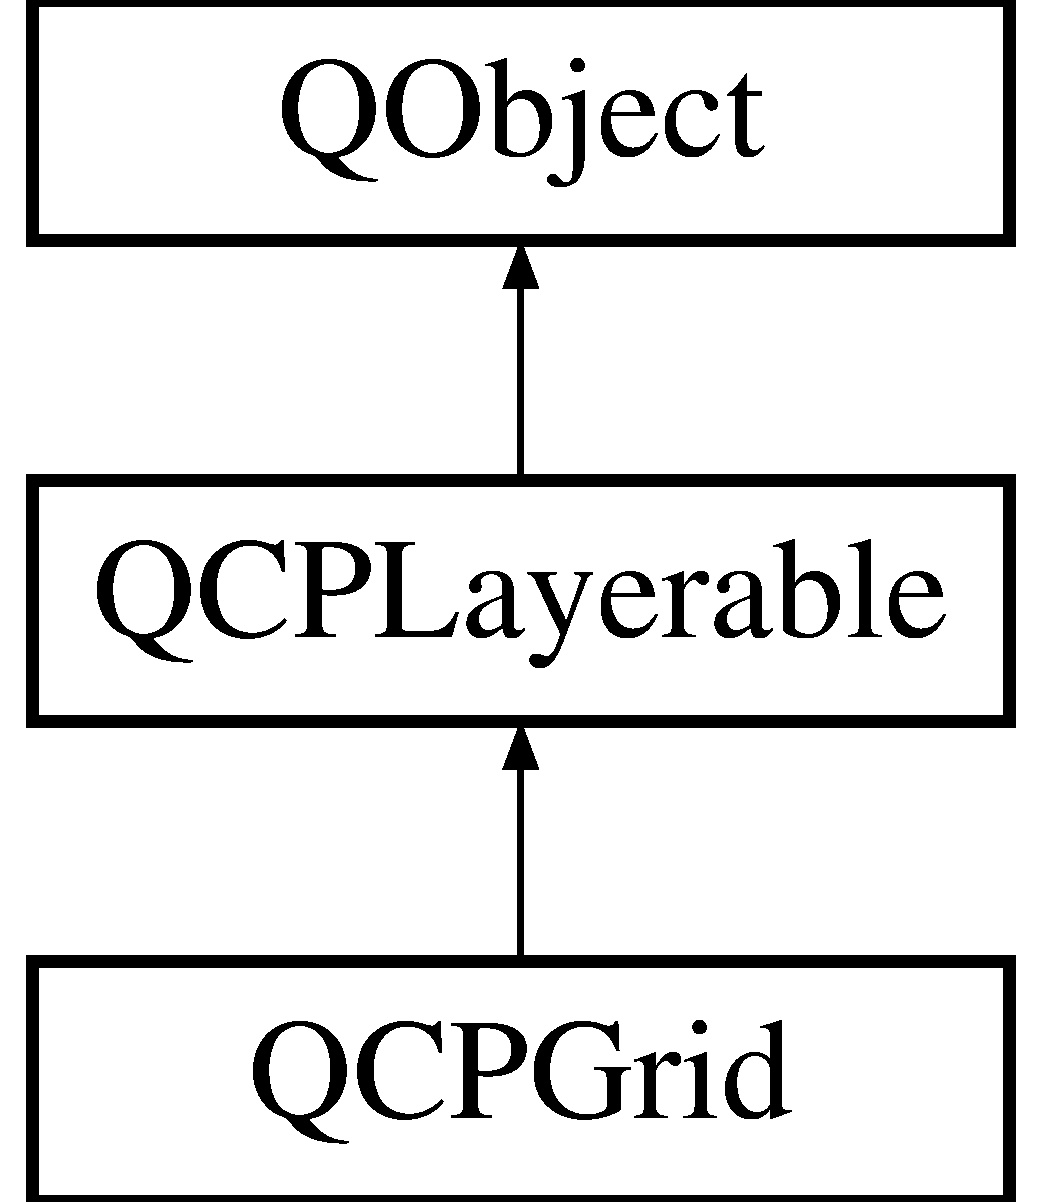
\includegraphics[height=3.000000cm]{class_q_c_p_grid}
\end{center}
\end{figure}
\subsection*{Public Member Functions}
\begin{DoxyCompactItemize}
\item 
\hyperlink{class_q_c_p_grid_acd1cdd2909625388a13048b698494a17}{Q\+C\+P\+Grid} (\hyperlink{class_q_c_p_axis}{Q\+C\+P\+Axis} $\ast$parent\+Axis)
\item 
\hypertarget{class_q_c_p_grid_afface6d8cb6df3cbdc0b5c7c2658f96a}{}\label{class_q_c_p_grid_afface6d8cb6df3cbdc0b5c7c2658f96a} 
bool {\bfseries sub\+Grid\+Visible} () const
\item 
\hypertarget{class_q_c_p_grid_af16a269b15b2a8d904be087d060536bc}{}\label{class_q_c_p_grid_af16a269b15b2a8d904be087d060536bc} 
bool {\bfseries antialiased\+Sub\+Grid} () const
\item 
\hypertarget{class_q_c_p_grid_a578d0bd4d2e5000a2ca69b9a034d59aa}{}\label{class_q_c_p_grid_a578d0bd4d2e5000a2ca69b9a034d59aa} 
bool {\bfseries antialiased\+Zero\+Line} () const
\item 
\hypertarget{class_q_c_p_grid_a1d68418766b3408c0b7b29ef40b04c2a}{}\label{class_q_c_p_grid_a1d68418766b3408c0b7b29ef40b04c2a} 
Q\+Pen {\bfseries pen} () const
\item 
\hypertarget{class_q_c_p_grid_ae231e5b87e68689a666f90531a15552f}{}\label{class_q_c_p_grid_ae231e5b87e68689a666f90531a15552f} 
Q\+Pen {\bfseries sub\+Grid\+Pen} () const
\item 
\hypertarget{class_q_c_p_grid_a85f248487110c4043be696aef5f2f6e1}{}\label{class_q_c_p_grid_a85f248487110c4043be696aef5f2f6e1} 
Q\+Pen {\bfseries zero\+Line\+Pen} () const
\item 
void \hyperlink{class_q_c_p_grid_ad4ad6bf714ec45e08845456355a1b700}{set\+Sub\+Grid\+Visible} (bool visible)
\item 
void \hyperlink{class_q_c_p_grid_a5692310ba183721a413d60951407d114}{set\+Antialiased\+Sub\+Grid} (bool enabled)
\item 
void \hyperlink{class_q_c_p_grid_a3cc6d54647393ee71afb6da56af07aa4}{set\+Antialiased\+Zero\+Line} (bool enabled)
\item 
void \hyperlink{class_q_c_p_grid_aa05ab9816ffb440908171e45e833b593}{set\+Pen} (const Q\+Pen \&pen)
\item 
void \hyperlink{class_q_c_p_grid_a9edd3593f384d1f0b0202a39cef4453d}{set\+Sub\+Grid\+Pen} (const Q\+Pen \&pen)
\item 
void \hyperlink{class_q_c_p_grid_a209f40fdb252397b418b82d3494d8ea0}{set\+Zero\+Line\+Pen} (const Q\+Pen \&pen)
\end{DoxyCompactItemize}
\subsection*{Protected Member Functions}
\begin{DoxyCompactItemize}
\item 
\hypertarget{class_q_c_p_grid_ac5d2c0a3b6212ce1c2c19f5a6df586e5}{}\label{class_q_c_p_grid_ac5d2c0a3b6212ce1c2c19f5a6df586e5} 
virtual void {\bfseries apply\+Default\+Antialiasing\+Hint} (\hyperlink{class_q_c_p_painter}{Q\+C\+P\+Painter} $\ast$painter) const
\item 
\hypertarget{class_q_c_p_grid_ad009c23f96078616aa4f66a750974b23}{}\label{class_q_c_p_grid_ad009c23f96078616aa4f66a750974b23} 
virtual void {\bfseries draw} (\hyperlink{class_q_c_p_painter}{Q\+C\+P\+Painter} $\ast$painter)
\item 
\hypertarget{class_q_c_p_grid_aee4e95d54acabbe298d6dda0dd86c0a4}{}\label{class_q_c_p_grid_aee4e95d54acabbe298d6dda0dd86c0a4} 
void {\bfseries draw\+Grid\+Lines} (\hyperlink{class_q_c_p_painter}{Q\+C\+P\+Painter} $\ast$painter) const
\item 
\hypertarget{class_q_c_p_grid_a751ce8aef815bcc9193432a30c8b6b6e}{}\label{class_q_c_p_grid_a751ce8aef815bcc9193432a30c8b6b6e} 
void {\bfseries draw\+Sub\+Grid\+Lines} (\hyperlink{class_q_c_p_painter}{Q\+C\+P\+Painter} $\ast$painter) const
\end{DoxyCompactItemize}
\subsection*{Protected Attributes}
\begin{DoxyCompactItemize}
\item 
\hypertarget{class_q_c_p_grid_a4e4a0400d6319bb44c06341f6298c87b}{}\label{class_q_c_p_grid_a4e4a0400d6319bb44c06341f6298c87b} 
bool {\bfseries m\+Sub\+Grid\+Visible}
\item 
\hypertarget{class_q_c_p_grid_a71b7051f833f0c5de3094998d6afdd87}{}\label{class_q_c_p_grid_a71b7051f833f0c5de3094998d6afdd87} 
bool {\bfseries m\+Antialiased\+Sub\+Grid}
\item 
\hypertarget{class_q_c_p_grid_a8c0df56ae86440408c050895dcdb922b}{}\label{class_q_c_p_grid_a8c0df56ae86440408c050895dcdb922b} 
bool {\bfseries m\+Antialiased\+Zero\+Line}
\item 
\hypertarget{class_q_c_p_grid_a1cdc4a3bccf6a40c2d4360def9fefa40}{}\label{class_q_c_p_grid_a1cdc4a3bccf6a40c2d4360def9fefa40} 
Q\+Pen {\bfseries m\+Pen}
\item 
\hypertarget{class_q_c_p_grid_aa9004bc139ad3ea92629f0aaae81d83f}{}\label{class_q_c_p_grid_aa9004bc139ad3ea92629f0aaae81d83f} 
Q\+Pen {\bfseries m\+Sub\+Grid\+Pen}
\item 
\hypertarget{class_q_c_p_grid_a379481871f17655c27eda30af233554f}{}\label{class_q_c_p_grid_a379481871f17655c27eda30af233554f} 
Q\+Pen {\bfseries m\+Zero\+Line\+Pen}
\item 
\hypertarget{class_q_c_p_grid_a9a8a76731e6e737b65b929fd1995cc88}{}\label{class_q_c_p_grid_a9a8a76731e6e737b65b929fd1995cc88} 
\hyperlink{class_q_c_p_axis}{Q\+C\+P\+Axis} $\ast$ {\bfseries m\+Parent\+Axis}
\end{DoxyCompactItemize}
\subsection*{Friends}
\begin{DoxyCompactItemize}
\item 
\hypertarget{class_q_c_p_grid_af123edeca169ec7a31958a1d714e1a8a}{}\label{class_q_c_p_grid_af123edeca169ec7a31958a1d714e1a8a} 
class {\bfseries Q\+C\+P\+Axis}
\end{DoxyCompactItemize}
\subsection*{Additional Inherited Members}


\subsection{Detailed Description}
Responsible for drawing the grid of a \hyperlink{class_q_c_p_axis}{Q\+C\+P\+Axis}. 

This class is tightly bound to \hyperlink{class_q_c_p_axis}{Q\+C\+P\+Axis}. Every axis owns a grid instance and uses it to draw the grid lines, sub grid lines and zero-\/line. You can interact with the grid of an axis via \hyperlink{class_q_c_p_axis_a63f1dd2df663680d2a8d06c19592dd63}{Q\+C\+P\+Axis\+::grid}. Normally, you don\textquotesingle{}t need to create an instance of \hyperlink{class_q_c_p_grid}{Q\+C\+P\+Grid} yourself.

The axis and grid drawing was split into two classes to allow them to be placed on different layers (both \hyperlink{class_q_c_p_axis}{Q\+C\+P\+Axis} and \hyperlink{class_q_c_p_grid}{Q\+C\+P\+Grid} inherit from \hyperlink{class_q_c_p_layerable}{Q\+C\+P\+Layerable}). Thus it is possible to have the grid in the background and the axes in the foreground, and any plottables/items in between. This described situation is the default setup, see the \hyperlink{class_q_c_p_layer}{Q\+C\+P\+Layer} documentation. 

\subsection{Constructor \& Destructor Documentation}
\hypertarget{class_q_c_p_grid_acd1cdd2909625388a13048b698494a17}{}\label{class_q_c_p_grid_acd1cdd2909625388a13048b698494a17} 
\index{Q\+C\+P\+Grid@{Q\+C\+P\+Grid}!Q\+C\+P\+Grid@{Q\+C\+P\+Grid}}
\index{Q\+C\+P\+Grid@{Q\+C\+P\+Grid}!Q\+C\+P\+Grid@{Q\+C\+P\+Grid}}
\subsubsection{\texorpdfstring{Q\+C\+P\+Grid()}{QCPGrid()}}
{\footnotesize\ttfamily Q\+C\+P\+Grid\+::\+Q\+C\+P\+Grid (\begin{DoxyParamCaption}\item[{\hyperlink{class_q_c_p_axis}{Q\+C\+P\+Axis} $\ast$}]{parent\+Axis }\end{DoxyParamCaption})}

Creates a \hyperlink{class_q_c_p_grid}{Q\+C\+P\+Grid} instance and sets default values.

You shouldn\textquotesingle{}t instantiate grids on their own, since every \hyperlink{class_q_c_p_axis}{Q\+C\+P\+Axis} brings its own \hyperlink{class_q_c_p_grid}{Q\+C\+P\+Grid}. 

\subsection{Member Function Documentation}
\hypertarget{class_q_c_p_grid_a5692310ba183721a413d60951407d114}{}\label{class_q_c_p_grid_a5692310ba183721a413d60951407d114} 
\index{Q\+C\+P\+Grid@{Q\+C\+P\+Grid}!set\+Antialiased\+Sub\+Grid@{set\+Antialiased\+Sub\+Grid}}
\index{set\+Antialiased\+Sub\+Grid@{set\+Antialiased\+Sub\+Grid}!Q\+C\+P\+Grid@{Q\+C\+P\+Grid}}
\subsubsection{\texorpdfstring{set\+Antialiased\+Sub\+Grid()}{setAntialiasedSubGrid()}}
{\footnotesize\ttfamily void Q\+C\+P\+Grid\+::set\+Antialiased\+Sub\+Grid (\begin{DoxyParamCaption}\item[{bool}]{enabled }\end{DoxyParamCaption})}

Sets whether sub grid lines are drawn antialiased. \hypertarget{class_q_c_p_grid_a3cc6d54647393ee71afb6da56af07aa4}{}\label{class_q_c_p_grid_a3cc6d54647393ee71afb6da56af07aa4} 
\index{Q\+C\+P\+Grid@{Q\+C\+P\+Grid}!set\+Antialiased\+Zero\+Line@{set\+Antialiased\+Zero\+Line}}
\index{set\+Antialiased\+Zero\+Line@{set\+Antialiased\+Zero\+Line}!Q\+C\+P\+Grid@{Q\+C\+P\+Grid}}
\subsubsection{\texorpdfstring{set\+Antialiased\+Zero\+Line()}{setAntialiasedZeroLine()}}
{\footnotesize\ttfamily void Q\+C\+P\+Grid\+::set\+Antialiased\+Zero\+Line (\begin{DoxyParamCaption}\item[{bool}]{enabled }\end{DoxyParamCaption})}

Sets whether zero lines are drawn antialiased. \hypertarget{class_q_c_p_grid_aa05ab9816ffb440908171e45e833b593}{}\label{class_q_c_p_grid_aa05ab9816ffb440908171e45e833b593} 
\index{Q\+C\+P\+Grid@{Q\+C\+P\+Grid}!set\+Pen@{set\+Pen}}
\index{set\+Pen@{set\+Pen}!Q\+C\+P\+Grid@{Q\+C\+P\+Grid}}
\subsubsection{\texorpdfstring{set\+Pen()}{setPen()}}
{\footnotesize\ttfamily void Q\+C\+P\+Grid\+::set\+Pen (\begin{DoxyParamCaption}\item[{const Q\+Pen \&}]{pen }\end{DoxyParamCaption})}

Sets the pen with which (major) grid lines are drawn. \hypertarget{class_q_c_p_grid_a9edd3593f384d1f0b0202a39cef4453d}{}\label{class_q_c_p_grid_a9edd3593f384d1f0b0202a39cef4453d} 
\index{Q\+C\+P\+Grid@{Q\+C\+P\+Grid}!set\+Sub\+Grid\+Pen@{set\+Sub\+Grid\+Pen}}
\index{set\+Sub\+Grid\+Pen@{set\+Sub\+Grid\+Pen}!Q\+C\+P\+Grid@{Q\+C\+P\+Grid}}
\subsubsection{\texorpdfstring{set\+Sub\+Grid\+Pen()}{setSubGridPen()}}
{\footnotesize\ttfamily void Q\+C\+P\+Grid\+::set\+Sub\+Grid\+Pen (\begin{DoxyParamCaption}\item[{const Q\+Pen \&}]{pen }\end{DoxyParamCaption})}

Sets the pen with which sub grid lines are drawn. \hypertarget{class_q_c_p_grid_ad4ad6bf714ec45e08845456355a1b700}{}\label{class_q_c_p_grid_ad4ad6bf714ec45e08845456355a1b700} 
\index{Q\+C\+P\+Grid@{Q\+C\+P\+Grid}!set\+Sub\+Grid\+Visible@{set\+Sub\+Grid\+Visible}}
\index{set\+Sub\+Grid\+Visible@{set\+Sub\+Grid\+Visible}!Q\+C\+P\+Grid@{Q\+C\+P\+Grid}}
\subsubsection{\texorpdfstring{set\+Sub\+Grid\+Visible()}{setSubGridVisible()}}
{\footnotesize\ttfamily void Q\+C\+P\+Grid\+::set\+Sub\+Grid\+Visible (\begin{DoxyParamCaption}\item[{bool}]{visible }\end{DoxyParamCaption})}

Sets whether grid lines at sub tick marks are drawn.

\begin{DoxySeeAlso}{See also}
\hyperlink{class_q_c_p_grid_a9edd3593f384d1f0b0202a39cef4453d}{set\+Sub\+Grid\+Pen} 
\end{DoxySeeAlso}
\hypertarget{class_q_c_p_grid_a209f40fdb252397b418b82d3494d8ea0}{}\label{class_q_c_p_grid_a209f40fdb252397b418b82d3494d8ea0} 
\index{Q\+C\+P\+Grid@{Q\+C\+P\+Grid}!set\+Zero\+Line\+Pen@{set\+Zero\+Line\+Pen}}
\index{set\+Zero\+Line\+Pen@{set\+Zero\+Line\+Pen}!Q\+C\+P\+Grid@{Q\+C\+P\+Grid}}
\subsubsection{\texorpdfstring{set\+Zero\+Line\+Pen()}{setZeroLinePen()}}
{\footnotesize\ttfamily void Q\+C\+P\+Grid\+::set\+Zero\+Line\+Pen (\begin{DoxyParamCaption}\item[{const Q\+Pen \&}]{pen }\end{DoxyParamCaption})}

Sets the pen with which zero lines are drawn.

Zero lines are lines at value coordinate 0 which may be drawn with a different pen than other grid lines. To disable zero lines and just draw normal grid lines at zero, set {\itshape pen} to Qt\+::\+No\+Pen. 

The documentation for this class was generated from the following files\+:\begin{DoxyCompactItemize}
\item 
C\+:/\+Users/\+Jesse Jutson/\+Documents/\+Git\+Hub/\+F\+E\+S\+S\+G\+U\+I/\+F\+E\+S\+S-\/\+G\+U\+I/\hyperlink{qcustomplot_8h}{qcustomplot.\+h}\item 
C\+:/\+Users/\+Jesse Jutson/\+Documents/\+Git\+Hub/\+F\+E\+S\+S\+G\+U\+I/\+F\+E\+S\+S-\/\+G\+U\+I/\hyperlink{qcustomplot_8cpp}{qcustomplot.\+cpp}\end{DoxyCompactItemize}

\hypertarget{class_q_c_p_item_anchor}{}\section{Q\+C\+P\+Item\+Anchor Class Reference}
\label{class_q_c_p_item_anchor}\index{Q\+C\+P\+Item\+Anchor@{Q\+C\+P\+Item\+Anchor}}


An anchor of an item to which positions can be attached to.  


Inheritance diagram for Q\+C\+P\+Item\+Anchor\+:\begin{figure}[H]
\begin{center}
\leavevmode
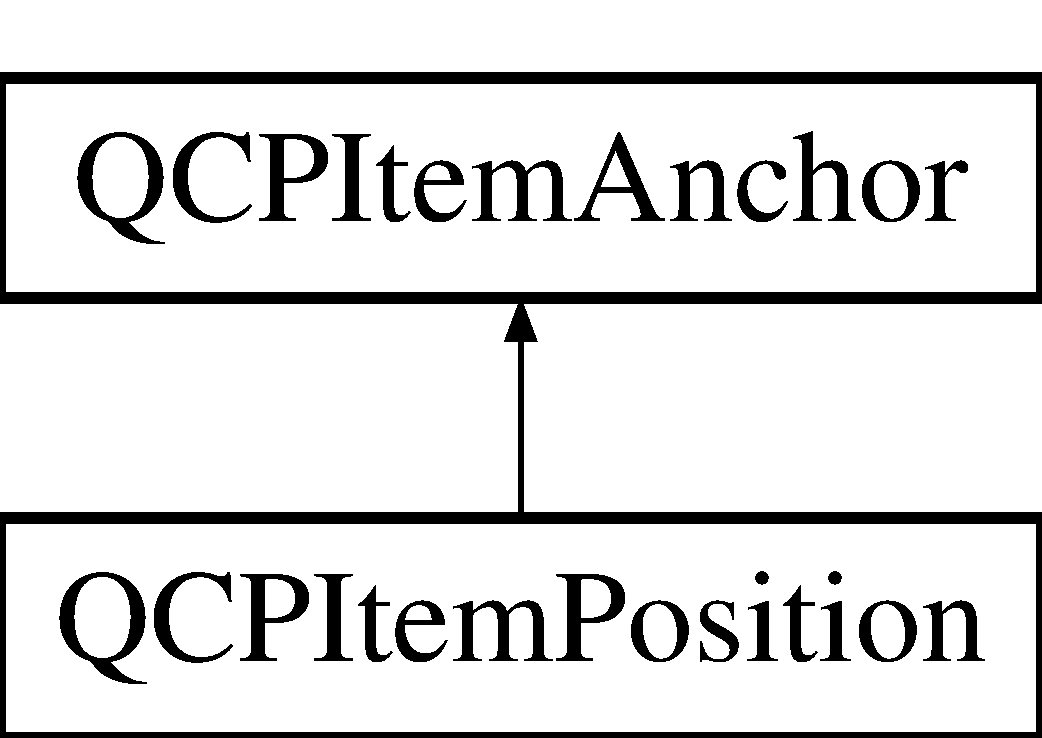
\includegraphics[height=2.000000cm]{class_q_c_p_item_anchor}
\end{center}
\end{figure}
\subsection*{Public Member Functions}
\begin{DoxyCompactItemize}
\item 
\hyperlink{class_q_c_p_item_anchor_aeb6b681d2bf324db40a915d32ec5624f}{Q\+C\+P\+Item\+Anchor} (\hyperlink{class_q_custom_plot}{Q\+Custom\+Plot} $\ast$parent\+Plot, \hyperlink{class_q_c_p_abstract_item}{Q\+C\+P\+Abstract\+Item} $\ast$parent\+Item, const Q\+String name, int anchor\+Id=-\/1)
\item 
\hypertarget{class_q_c_p_item_anchor_aad37cdf5a3f63428f61be739014e212e}{}\label{class_q_c_p_item_anchor_aad37cdf5a3f63428f61be739014e212e} 
Q\+String {\bfseries name} () const
\item 
virtual Q\+PointF \hyperlink{class_q_c_p_item_anchor_ae1a21d9471d1d788624cad297e1b8d6f}{pixel\+Point} () const
\end{DoxyCompactItemize}
\subsection*{Protected Member Functions}
\begin{DoxyCompactItemize}
\item 
virtual \hyperlink{class_q_c_p_item_position}{Q\+C\+P\+Item\+Position} $\ast$ \hyperlink{class_q_c_p_item_anchor_ac54b20120669950255a63587193dbb86}{to\+Q\+C\+P\+Item\+Position} ()
\item 
\hypertarget{class_q_c_p_item_anchor_aef15daa640debfb11b0aeaa2116c6fbc}{}\label{class_q_c_p_item_anchor_aef15daa640debfb11b0aeaa2116c6fbc} 
void {\bfseries add\+ChildX} (\hyperlink{class_q_c_p_item_position}{Q\+C\+P\+Item\+Position} $\ast$pos)
\item 
\hypertarget{class_q_c_p_item_anchor_a230b1d494cda63458e289bbe1b642599}{}\label{class_q_c_p_item_anchor_a230b1d494cda63458e289bbe1b642599} 
void {\bfseries remove\+ChildX} (\hyperlink{class_q_c_p_item_position}{Q\+C\+P\+Item\+Position} $\ast$pos)
\item 
\hypertarget{class_q_c_p_item_anchor_af05dc56f24536f0c7a9a0f57b58cea67}{}\label{class_q_c_p_item_anchor_af05dc56f24536f0c7a9a0f57b58cea67} 
void {\bfseries add\+ChildY} (\hyperlink{class_q_c_p_item_position}{Q\+C\+P\+Item\+Position} $\ast$pos)
\item 
\hypertarget{class_q_c_p_item_anchor_aa2394911d8fff3bd958b9f4f1994b64d}{}\label{class_q_c_p_item_anchor_aa2394911d8fff3bd958b9f4f1994b64d} 
void {\bfseries remove\+ChildY} (\hyperlink{class_q_c_p_item_position}{Q\+C\+P\+Item\+Position} $\ast$pos)
\end{DoxyCompactItemize}
\subsection*{Protected Attributes}
\begin{DoxyCompactItemize}
\item 
\hypertarget{class_q_c_p_item_anchor_a23ad4d0ab0d2cbb41a7baf05bcf996ec}{}\label{class_q_c_p_item_anchor_a23ad4d0ab0d2cbb41a7baf05bcf996ec} 
Q\+String {\bfseries m\+Name}
\item 
\hypertarget{class_q_c_p_item_anchor_a59b968410831ba91a25cc75a77dde6f5}{}\label{class_q_c_p_item_anchor_a59b968410831ba91a25cc75a77dde6f5} 
\hyperlink{class_q_custom_plot}{Q\+Custom\+Plot} $\ast$ {\bfseries m\+Parent\+Plot}
\item 
\hypertarget{class_q_c_p_item_anchor_a80fad480ad3bb980446ed6ebc00818ae}{}\label{class_q_c_p_item_anchor_a80fad480ad3bb980446ed6ebc00818ae} 
\hyperlink{class_q_c_p_abstract_item}{Q\+C\+P\+Abstract\+Item} $\ast$ {\bfseries m\+Parent\+Item}
\item 
\hypertarget{class_q_c_p_item_anchor_a00c62070333e8345976b579676ad3997}{}\label{class_q_c_p_item_anchor_a00c62070333e8345976b579676ad3997} 
int {\bfseries m\+Anchor\+Id}
\item 
\hypertarget{class_q_c_p_item_anchor_a3c0bfd6e50f3b48e2a9b3824695b20f7}{}\label{class_q_c_p_item_anchor_a3c0bfd6e50f3b48e2a9b3824695b20f7} 
Q\+Set$<$ \hyperlink{class_q_c_p_item_position}{Q\+C\+P\+Item\+Position} $\ast$ $>$ {\bfseries m\+ChildrenX}
\item 
\hypertarget{class_q_c_p_item_anchor_a3abe4eebd0683454d81c8341df6f7115}{}\label{class_q_c_p_item_anchor_a3abe4eebd0683454d81c8341df6f7115} 
Q\+Set$<$ \hyperlink{class_q_c_p_item_position}{Q\+C\+P\+Item\+Position} $\ast$ $>$ {\bfseries m\+ChildrenY}
\end{DoxyCompactItemize}
\subsection*{Friends}
\begin{DoxyCompactItemize}
\item 
\hypertarget{class_q_c_p_item_anchor_aa9b8ddc062778e202a0be06a57d18d17}{}\label{class_q_c_p_item_anchor_aa9b8ddc062778e202a0be06a57d18d17} 
class {\bfseries Q\+C\+P\+Item\+Position}
\end{DoxyCompactItemize}


\subsection{Detailed Description}
An anchor of an item to which positions can be attached to. 

An item (\hyperlink{class_q_c_p_abstract_item}{Q\+C\+P\+Abstract\+Item}) may have one or more anchors. Unlike \hyperlink{class_q_c_p_item_position}{Q\+C\+P\+Item\+Position}, an anchor doesn\textquotesingle{}t control anything on its item, but provides a way to tie other items via their positions to the anchor.

For example, a \hyperlink{class_q_c_p_item_rect}{Q\+C\+P\+Item\+Rect} is defined by its positions {\itshape top\+Left} and {\itshape bottom\+Right}. Additionally it has various anchors like {\itshape top}, {\itshape top\+Right} or {\itshape bottom\+Left} etc. So you can attach the {\itshape start} (which is a \hyperlink{class_q_c_p_item_position}{Q\+C\+P\+Item\+Position}) of a \hyperlink{class_q_c_p_item_line}{Q\+C\+P\+Item\+Line} to one of the anchors by calling \hyperlink{class_q_c_p_item_position_ac094d67a95d2dceafa0d50b9db3a7e51}{Q\+C\+P\+Item\+Position\+::set\+Parent\+Anchor} on {\itshape start}, passing the wanted anchor of the \hyperlink{class_q_c_p_item_rect}{Q\+C\+P\+Item\+Rect}. This way the start of the line will now always follow the respective anchor location on the rect item.

Note that \hyperlink{class_q_c_p_item_position}{Q\+C\+P\+Item\+Position} derives from \hyperlink{class_q_c_p_item_anchor}{Q\+C\+P\+Item\+Anchor}, so every position can also serve as an anchor to other positions.

To learn how to provide anchors in your own item subclasses, see the subclassing section of the \hyperlink{class_q_c_p_abstract_item}{Q\+C\+P\+Abstract\+Item} documentation. 

\subsection{Constructor \& Destructor Documentation}
\hypertarget{class_q_c_p_item_anchor_aeb6b681d2bf324db40a915d32ec5624f}{}\label{class_q_c_p_item_anchor_aeb6b681d2bf324db40a915d32ec5624f} 
\index{Q\+C\+P\+Item\+Anchor@{Q\+C\+P\+Item\+Anchor}!Q\+C\+P\+Item\+Anchor@{Q\+C\+P\+Item\+Anchor}}
\index{Q\+C\+P\+Item\+Anchor@{Q\+C\+P\+Item\+Anchor}!Q\+C\+P\+Item\+Anchor@{Q\+C\+P\+Item\+Anchor}}
\subsubsection{\texorpdfstring{Q\+C\+P\+Item\+Anchor()}{QCPItemAnchor()}}
{\footnotesize\ttfamily Q\+C\+P\+Item\+Anchor\+::\+Q\+C\+P\+Item\+Anchor (\begin{DoxyParamCaption}\item[{\hyperlink{class_q_custom_plot}{Q\+Custom\+Plot} $\ast$}]{parent\+Plot,  }\item[{\hyperlink{class_q_c_p_abstract_item}{Q\+C\+P\+Abstract\+Item} $\ast$}]{parent\+Item,  }\item[{const Q\+String}]{name,  }\item[{int}]{anchor\+Id = {\ttfamily -\/1} }\end{DoxyParamCaption})}

Creates a new \hyperlink{class_q_c_p_item_anchor}{Q\+C\+P\+Item\+Anchor}. You shouldn\textquotesingle{}t create \hyperlink{class_q_c_p_item_anchor}{Q\+C\+P\+Item\+Anchor} instances directly, even if you want to make a new item subclass. Use Q\+C\+P\+Abstract\+Item\+::create\+Anchor instead, as explained in the subclassing section of the \hyperlink{class_q_c_p_abstract_item}{Q\+C\+P\+Abstract\+Item} documentation. 

\subsection{Member Function Documentation}
\hypertarget{class_q_c_p_item_anchor_ae1a21d9471d1d788624cad297e1b8d6f}{}\label{class_q_c_p_item_anchor_ae1a21d9471d1d788624cad297e1b8d6f} 
\index{Q\+C\+P\+Item\+Anchor@{Q\+C\+P\+Item\+Anchor}!pixel\+Point@{pixel\+Point}}
\index{pixel\+Point@{pixel\+Point}!Q\+C\+P\+Item\+Anchor@{Q\+C\+P\+Item\+Anchor}}
\subsubsection{\texorpdfstring{pixel\+Point()}{pixelPoint()}}
{\footnotesize\ttfamily Q\+PointF Q\+C\+P\+Item\+Anchor\+::pixel\+Point (\begin{DoxyParamCaption}{ }\end{DoxyParamCaption}) const\hspace{0.3cm}{\ttfamily [virtual]}}

Returns the final absolute pixel position of the \hyperlink{class_q_c_p_item_anchor}{Q\+C\+P\+Item\+Anchor} on the \hyperlink{class_q_custom_plot}{Q\+Custom\+Plot} surface.

The pixel information is internally retrieved via Q\+C\+P\+Abstract\+Item\+::anchor\+Pixel\+Position of the parent item, \hyperlink{class_q_c_p_item_anchor}{Q\+C\+P\+Item\+Anchor} is just an intermediary. 

Reimplemented in \hyperlink{class_q_c_p_item_position_a6cad070c22801295231f5bd6045afe70}{Q\+C\+P\+Item\+Position}.

\hypertarget{class_q_c_p_item_anchor_ac54b20120669950255a63587193dbb86}{}\label{class_q_c_p_item_anchor_ac54b20120669950255a63587193dbb86} 
\index{Q\+C\+P\+Item\+Anchor@{Q\+C\+P\+Item\+Anchor}!to\+Q\+C\+P\+Item\+Position@{to\+Q\+C\+P\+Item\+Position}}
\index{to\+Q\+C\+P\+Item\+Position@{to\+Q\+C\+P\+Item\+Position}!Q\+C\+P\+Item\+Anchor@{Q\+C\+P\+Item\+Anchor}}
\subsubsection{\texorpdfstring{to\+Q\+C\+P\+Item\+Position()}{toQCPItemPosition()}}
{\footnotesize\ttfamily \hyperlink{class_q_c_p_item_position}{Q\+C\+P\+Item\+Position} $\ast$ Q\+C\+P\+Item\+Anchor\+::to\+Q\+C\+P\+Item\+Position (\begin{DoxyParamCaption}{ }\end{DoxyParamCaption})\hspace{0.3cm}{\ttfamily [inline]}, {\ttfamily [protected]}, {\ttfamily [virtual]}}

Returns 0 if this instance is merely a \hyperlink{class_q_c_p_item_anchor}{Q\+C\+P\+Item\+Anchor}, and a valid pointer of type Q\+C\+P\+Item\+Position$\ast$ if it actually is a \hyperlink{class_q_c_p_item_position}{Q\+C\+P\+Item\+Position} (which is a subclass of \hyperlink{class_q_c_p_item_anchor}{Q\+C\+P\+Item\+Anchor}).

This safe downcast functionality could also be achieved with a dynamic\+\_\+cast. However, \hyperlink{class_q_custom_plot}{Q\+Custom\+Plot} avoids dynamic\+\_\+cast to work with projects that don\textquotesingle{}t have R\+T\+TI support enabled (e.\+g. -\/fno-\/rtti flag with gcc compiler). 

Reimplemented in \hyperlink{class_q_c_p_item_position_a577a7efc601df85a20b3e709d1ac320e}{Q\+C\+P\+Item\+Position}.



The documentation for this class was generated from the following files\+:\begin{DoxyCompactItemize}
\item 
C\+:/\+Users/\+Jesse Jutson/\+Documents/\+Git\+Hub/\+F\+E\+S\+S\+G\+U\+I/\+F\+E\+S\+S-\/\+G\+U\+I/\hyperlink{qcustomplot_8h}{qcustomplot.\+h}\item 
C\+:/\+Users/\+Jesse Jutson/\+Documents/\+Git\+Hub/\+F\+E\+S\+S\+G\+U\+I/\+F\+E\+S\+S-\/\+G\+U\+I/\hyperlink{qcustomplot_8cpp}{qcustomplot.\+cpp}\end{DoxyCompactItemize}

\hypertarget{class_q_c_p_item_bracket}{}\section{Q\+C\+P\+Item\+Bracket Class Reference}
\label{class_q_c_p_item_bracket}\index{Q\+C\+P\+Item\+Bracket@{Q\+C\+P\+Item\+Bracket}}


A bracket for referencing/highlighting certain parts in the plot.  


Inheritance diagram for Q\+C\+P\+Item\+Bracket\+:\begin{figure}[H]
\begin{center}
\leavevmode
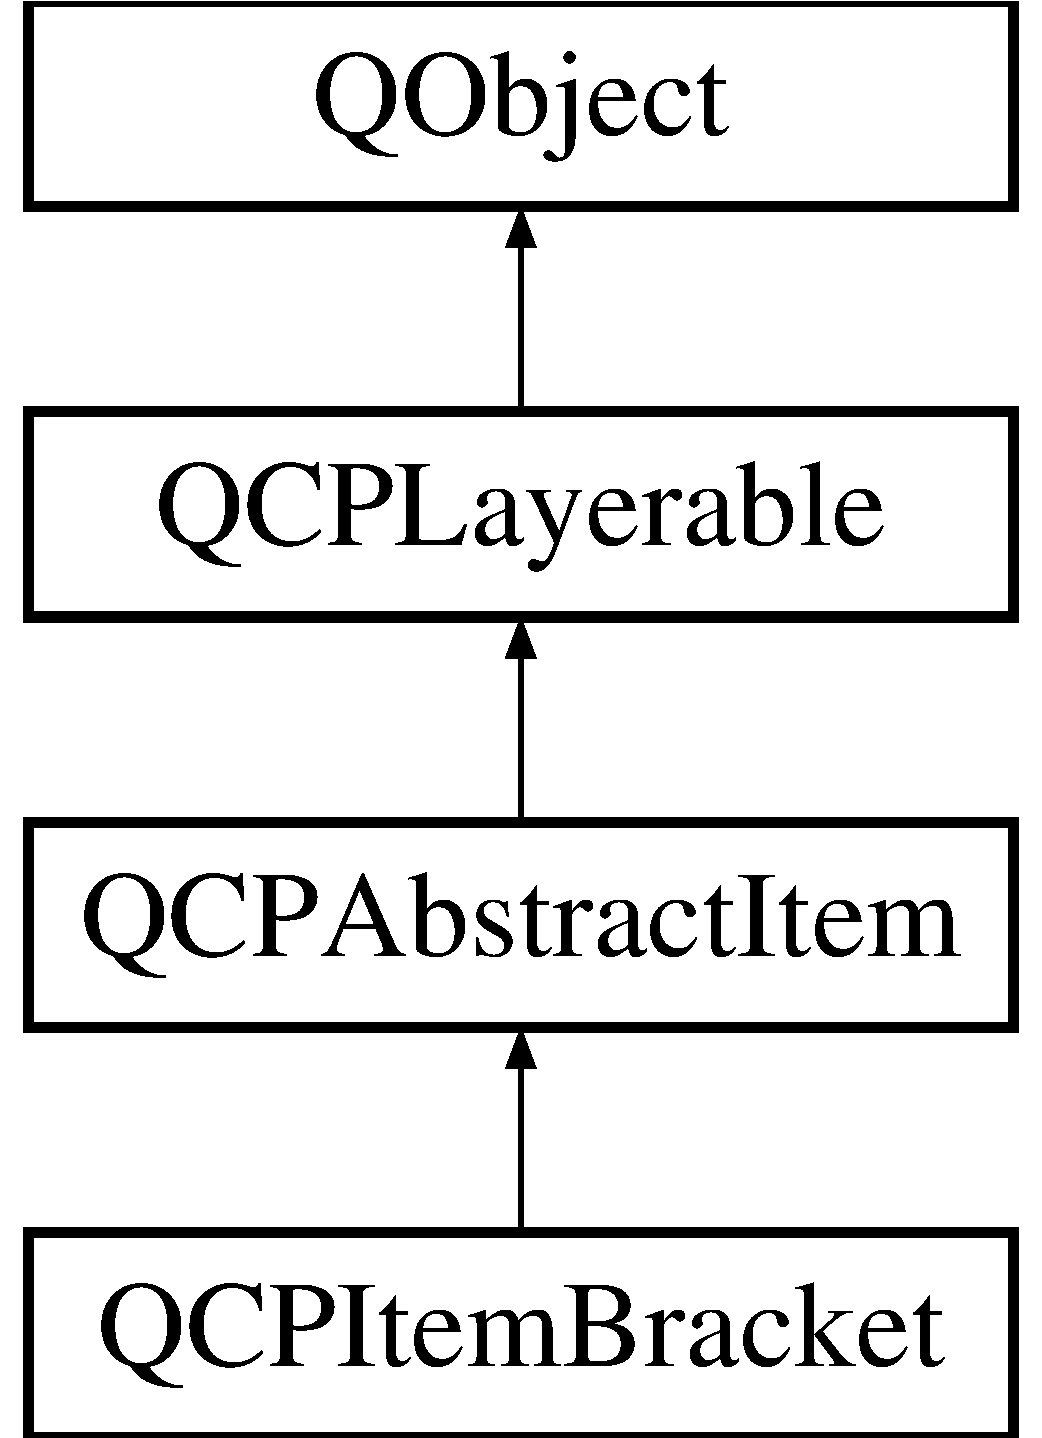
\includegraphics[height=4.000000cm]{class_q_c_p_item_bracket}
\end{center}
\end{figure}
\subsection*{Public Types}
\begin{DoxyCompactItemize}
\item 
enum \hyperlink{class_q_c_p_item_bracket_a7ac3afd0b24a607054e7212047d59dbd}{Bracket\+Style} \{ \hyperlink{class_q_c_p_item_bracket_a7ac3afd0b24a607054e7212047d59dbda7f9df4a7359bfe3dac1dbe4ccf5d220c}{bs\+Square}, 
\hyperlink{class_q_c_p_item_bracket_a7ac3afd0b24a607054e7212047d59dbda394627b0830a26ee3e0a02ca67a9f918}{bs\+Round}, 
\hyperlink{class_q_c_p_item_bracket_a7ac3afd0b24a607054e7212047d59dbda5024ce4023c2d8de4221f1cd4816acd8}{bs\+Curly}, 
\hyperlink{class_q_c_p_item_bracket_a7ac3afd0b24a607054e7212047d59dbda8f29f5ef754e2dc9a9efdedb2face0f3}{bs\+Calligraphic}
 \}
\end{DoxyCompactItemize}
\subsection*{Public Member Functions}
\begin{DoxyCompactItemize}
\item 
\hyperlink{class_q_c_p_item_bracket_a44ecfa37a76de5e3549e2d61f9d8ee56}{Q\+C\+P\+Item\+Bracket} (\hyperlink{class_q_custom_plot}{Q\+Custom\+Plot} $\ast$parent\+Plot)
\item 
\hypertarget{class_q_c_p_item_bracket_a6013b3f83aab7bc82b485ee5447ecb1b}{}\label{class_q_c_p_item_bracket_a6013b3f83aab7bc82b485ee5447ecb1b} 
Q\+Pen {\bfseries pen} () const
\item 
\hypertarget{class_q_c_p_item_bracket_aff5318a5415b87d9753c84752c65dd14}{}\label{class_q_c_p_item_bracket_aff5318a5415b87d9753c84752c65dd14} 
Q\+Pen {\bfseries selected\+Pen} () const
\item 
\hypertarget{class_q_c_p_item_bracket_af69dbe7ca5847f36403e1fb502e8e59d}{}\label{class_q_c_p_item_bracket_af69dbe7ca5847f36403e1fb502e8e59d} 
double {\bfseries length} () const
\item 
\hypertarget{class_q_c_p_item_bracket_a600ad8c0a3193cc2f335db6039f2932d}{}\label{class_q_c_p_item_bracket_a600ad8c0a3193cc2f335db6039f2932d} 
\hyperlink{class_q_c_p_item_bracket_a7ac3afd0b24a607054e7212047d59dbd}{Bracket\+Style} {\bfseries style} () const
\item 
void \hyperlink{class_q_c_p_item_bracket_ab13001d9cc5d8f9e56ea15bdda682acb}{set\+Pen} (const Q\+Pen \&pen)
\item 
void \hyperlink{class_q_c_p_item_bracket_a349785c31122778a520c64891fa204c5}{set\+Selected\+Pen} (const Q\+Pen \&pen)
\item 
void \hyperlink{class_q_c_p_item_bracket_ac7cfc3da7da9b5c5ac5dfbe4f0351b2a}{set\+Length} (double length)
\item 
void \hyperlink{class_q_c_p_item_bracket_a612dffa2373422eef8754d690add3703}{set\+Style} (\hyperlink{class_q_c_p_item_bracket_a7ac3afd0b24a607054e7212047d59dbd}{Bracket\+Style} style)
\item 
virtual double \hyperlink{class_q_c_p_item_bracket_a971299aa6fef75730d6f10efdaf48616}{select\+Test} (const Q\+PointF \&pos, bool only\+Selectable, Q\+Variant $\ast$details=0) const
\end{DoxyCompactItemize}
\subsection*{Public Attributes}
\begin{DoxyCompactItemize}
\item 
\hypertarget{class_q_c_p_item_bracket_af6cc6d27d96171778c6927d6edce48b0}{}\label{class_q_c_p_item_bracket_af6cc6d27d96171778c6927d6edce48b0} 
\hyperlink{class_q_c_p_item_position}{Q\+C\+P\+Item\+Position} $\ast$const {\bfseries left}
\item 
\hypertarget{class_q_c_p_item_bracket_afa6c1360b05a50c4e0df37b3cebab6be}{}\label{class_q_c_p_item_bracket_afa6c1360b05a50c4e0df37b3cebab6be} 
\hyperlink{class_q_c_p_item_position}{Q\+C\+P\+Item\+Position} $\ast$const {\bfseries right}
\item 
\hypertarget{class_q_c_p_item_bracket_a2dbcabdf5f467f28be12a7b25962ffca}{}\label{class_q_c_p_item_bracket_a2dbcabdf5f467f28be12a7b25962ffca} 
\hyperlink{class_q_c_p_item_anchor}{Q\+C\+P\+Item\+Anchor} $\ast$const {\bfseries center}
\end{DoxyCompactItemize}
\subsection*{Protected Types}
\begin{DoxyCompactItemize}
\item 
\hypertarget{class_q_c_p_item_bracket_a7f3a6a56d67f71219ed220553f3dd861}{}\label{class_q_c_p_item_bracket_a7f3a6a56d67f71219ed220553f3dd861} 
enum {\bfseries Anchor\+Index} \{ {\bfseries ai\+Center}
 \}
\end{DoxyCompactItemize}
\subsection*{Protected Member Functions}
\begin{DoxyCompactItemize}
\item 
\hypertarget{class_q_c_p_item_bracket_a8343cf0559c64886add7aa7f4b22f1a6}{}\label{class_q_c_p_item_bracket_a8343cf0559c64886add7aa7f4b22f1a6} 
virtual void {\bfseries draw} (\hyperlink{class_q_c_p_painter}{Q\+C\+P\+Painter} $\ast$painter)
\item 
\hypertarget{class_q_c_p_item_bracket_a4ad167aab5d38e173171f0afc14a5dd3}{}\label{class_q_c_p_item_bracket_a4ad167aab5d38e173171f0afc14a5dd3} 
virtual Q\+PointF {\bfseries anchor\+Pixel\+Point} (int anchor\+Id) const
\item 
\hypertarget{class_q_c_p_item_bracket_af1c445df1a574bddc8a40efcd76dd2e1}{}\label{class_q_c_p_item_bracket_af1c445df1a574bddc8a40efcd76dd2e1} 
Q\+Pen {\bfseries main\+Pen} () const
\end{DoxyCompactItemize}
\subsection*{Protected Attributes}
\begin{DoxyCompactItemize}
\item 
\hypertarget{class_q_c_p_item_bracket_a350c864a5853b04343719f5a8be6b675}{}\label{class_q_c_p_item_bracket_a350c864a5853b04343719f5a8be6b675} 
Q\+Pen {\bfseries m\+Pen}
\item 
\hypertarget{class_q_c_p_item_bracket_adcfb53602d1802d00e2de4fd6df6b291}{}\label{class_q_c_p_item_bracket_adcfb53602d1802d00e2de4fd6df6b291} 
Q\+Pen {\bfseries m\+Selected\+Pen}
\item 
\hypertarget{class_q_c_p_item_bracket_ab3d99bba8da18eb4d0e0cb23dded33b2}{}\label{class_q_c_p_item_bracket_ab3d99bba8da18eb4d0e0cb23dded33b2} 
double {\bfseries m\+Length}
\item 
\hypertarget{class_q_c_p_item_bracket_ac911907184c824d621f274f8e0990080}{}\label{class_q_c_p_item_bracket_ac911907184c824d621f274f8e0990080} 
\hyperlink{class_q_c_p_item_bracket_a7ac3afd0b24a607054e7212047d59dbd}{Bracket\+Style} {\bfseries m\+Style}
\end{DoxyCompactItemize}
\subsection*{Additional Inherited Members}


\subsection{Detailed Description}
A bracket for referencing/highlighting certain parts in the plot. 

 It has two positions, {\itshape left} and {\itshape right}, which define the span of the bracket. If {\itshape left} is actually farther to the left than {\itshape right}, the bracket is opened to the bottom, as shown in the example image.

The bracket supports multiple styles via \hyperlink{class_q_c_p_item_bracket_a612dffa2373422eef8754d690add3703}{set\+Style}. The length, i.\+e. how far the bracket stretches away from the embraced span, can be controlled with \hyperlink{class_q_c_p_item_bracket_ac7cfc3da7da9b5c5ac5dfbe4f0351b2a}{set\+Length}.

 \begin{center}Demonstrating the effect of different values for \hyperlink{class_q_c_p_item_bracket_ac7cfc3da7da9b5c5ac5dfbe4f0351b2a}{set\+Length}, for styles \hyperlink{class_q_c_p_item_bracket_a7ac3afd0b24a607054e7212047d59dbda8f29f5ef754e2dc9a9efdedb2face0f3}{bs\+Calligraphic} and \hyperlink{class_q_c_p_item_bracket_a7ac3afd0b24a607054e7212047d59dbda7f9df4a7359bfe3dac1dbe4ccf5d220c}{bs\+Square}. Anchors and positions are displayed for reference.\end{center} 

It provides an anchor {\itshape center}, to allow connection of other items, e.\+g. an arrow (\hyperlink{class_q_c_p_item_line}{Q\+C\+P\+Item\+Line} or \hyperlink{class_q_c_p_item_curve}{Q\+C\+P\+Item\+Curve}) or a text label (\hyperlink{class_q_c_p_item_text}{Q\+C\+P\+Item\+Text}), to the bracket. 

\subsection{Member Enumeration Documentation}
\hypertarget{class_q_c_p_item_bracket_a7ac3afd0b24a607054e7212047d59dbd}{}\label{class_q_c_p_item_bracket_a7ac3afd0b24a607054e7212047d59dbd} 
\index{Q\+C\+P\+Item\+Bracket@{Q\+C\+P\+Item\+Bracket}!Bracket\+Style@{Bracket\+Style}}
\index{Bracket\+Style@{Bracket\+Style}!Q\+C\+P\+Item\+Bracket@{Q\+C\+P\+Item\+Bracket}}
\subsubsection{\texorpdfstring{Bracket\+Style}{BracketStyle}}
{\footnotesize\ttfamily enum \hyperlink{class_q_c_p_item_bracket_a7ac3afd0b24a607054e7212047d59dbd}{Q\+C\+P\+Item\+Bracket\+::\+Bracket\+Style}}

\begin{DoxyEnumFields}{Enumerator}
\raisebox{\heightof{T}}[0pt][0pt]{\index{bs\+Square@{bs\+Square}!Q\+C\+P\+Item\+Bracket@{Q\+C\+P\+Item\+Bracket}}\index{Q\+C\+P\+Item\+Bracket@{Q\+C\+P\+Item\+Bracket}!bs\+Square@{bs\+Square}}}\hypertarget{class_q_c_p_item_bracket_a7ac3afd0b24a607054e7212047d59dbda7f9df4a7359bfe3dac1dbe4ccf5d220c}{}\label{class_q_c_p_item_bracket_a7ac3afd0b24a607054e7212047d59dbda7f9df4a7359bfe3dac1dbe4ccf5d220c} 
bs\+Square&A brace with angled edges. \\
\hline

\raisebox{\heightof{T}}[0pt][0pt]{\index{bs\+Round@{bs\+Round}!Q\+C\+P\+Item\+Bracket@{Q\+C\+P\+Item\+Bracket}}\index{Q\+C\+P\+Item\+Bracket@{Q\+C\+P\+Item\+Bracket}!bs\+Round@{bs\+Round}}}\hypertarget{class_q_c_p_item_bracket_a7ac3afd0b24a607054e7212047d59dbda394627b0830a26ee3e0a02ca67a9f918}{}\label{class_q_c_p_item_bracket_a7ac3afd0b24a607054e7212047d59dbda394627b0830a26ee3e0a02ca67a9f918} 
bs\+Round&A brace with round edges. \\
\hline

\raisebox{\heightof{T}}[0pt][0pt]{\index{bs\+Curly@{bs\+Curly}!Q\+C\+P\+Item\+Bracket@{Q\+C\+P\+Item\+Bracket}}\index{Q\+C\+P\+Item\+Bracket@{Q\+C\+P\+Item\+Bracket}!bs\+Curly@{bs\+Curly}}}\hypertarget{class_q_c_p_item_bracket_a7ac3afd0b24a607054e7212047d59dbda5024ce4023c2d8de4221f1cd4816acd8}{}\label{class_q_c_p_item_bracket_a7ac3afd0b24a607054e7212047d59dbda5024ce4023c2d8de4221f1cd4816acd8} 
bs\+Curly&A curly brace. \\
\hline

\raisebox{\heightof{T}}[0pt][0pt]{\index{bs\+Calligraphic@{bs\+Calligraphic}!Q\+C\+P\+Item\+Bracket@{Q\+C\+P\+Item\+Bracket}}\index{Q\+C\+P\+Item\+Bracket@{Q\+C\+P\+Item\+Bracket}!bs\+Calligraphic@{bs\+Calligraphic}}}\hypertarget{class_q_c_p_item_bracket_a7ac3afd0b24a607054e7212047d59dbda8f29f5ef754e2dc9a9efdedb2face0f3}{}\label{class_q_c_p_item_bracket_a7ac3afd0b24a607054e7212047d59dbda8f29f5ef754e2dc9a9efdedb2face0f3} 
bs\+Calligraphic&A curly brace with varying stroke width giving a calligraphic impression. \\
\hline

\end{DoxyEnumFields}


\subsection{Constructor \& Destructor Documentation}
\hypertarget{class_q_c_p_item_bracket_a44ecfa37a76de5e3549e2d61f9d8ee56}{}\label{class_q_c_p_item_bracket_a44ecfa37a76de5e3549e2d61f9d8ee56} 
\index{Q\+C\+P\+Item\+Bracket@{Q\+C\+P\+Item\+Bracket}!Q\+C\+P\+Item\+Bracket@{Q\+C\+P\+Item\+Bracket}}
\index{Q\+C\+P\+Item\+Bracket@{Q\+C\+P\+Item\+Bracket}!Q\+C\+P\+Item\+Bracket@{Q\+C\+P\+Item\+Bracket}}
\subsubsection{\texorpdfstring{Q\+C\+P\+Item\+Bracket()}{QCPItemBracket()}}
{\footnotesize\ttfamily Q\+C\+P\+Item\+Bracket\+::\+Q\+C\+P\+Item\+Bracket (\begin{DoxyParamCaption}\item[{\hyperlink{class_q_custom_plot}{Q\+Custom\+Plot} $\ast$}]{parent\+Plot }\end{DoxyParamCaption})}

Creates a bracket item and sets default values.

The constructed item can be added to the plot with \hyperlink{class_q_custom_plot_aa500620379262321685cb7a7674cbd2a}{Q\+Custom\+Plot\+::add\+Item}. 

\subsection{Member Function Documentation}
\hypertarget{class_q_c_p_item_bracket_a971299aa6fef75730d6f10efdaf48616}{}\label{class_q_c_p_item_bracket_a971299aa6fef75730d6f10efdaf48616} 
\index{Q\+C\+P\+Item\+Bracket@{Q\+C\+P\+Item\+Bracket}!select\+Test@{select\+Test}}
\index{select\+Test@{select\+Test}!Q\+C\+P\+Item\+Bracket@{Q\+C\+P\+Item\+Bracket}}
\subsubsection{\texorpdfstring{select\+Test()}{selectTest()}}
{\footnotesize\ttfamily double Q\+C\+P\+Item\+Bracket\+::select\+Test (\begin{DoxyParamCaption}\item[{const Q\+PointF \&}]{pos,  }\item[{bool}]{only\+Selectable,  }\item[{Q\+Variant $\ast$}]{details = {\ttfamily 0} }\end{DoxyParamCaption}) const\hspace{0.3cm}{\ttfamily [virtual]}}

This function is used to decide whether a click hits a layerable object or not.

{\itshape pos} is a point in pixel coordinates on the \hyperlink{class_q_custom_plot}{Q\+Custom\+Plot} surface. This function returns the shortest pixel distance of this point to the object. If the object is either invisible or the distance couldn\textquotesingle{}t be determined, -\/1.\+0 is returned. Further, if {\itshape only\+Selectable} is true and the object is not selectable, -\/1.\+0 is returned, too.

If the object is represented not by single lines but by an area like a \hyperlink{class_q_c_p_item_text}{Q\+C\+P\+Item\+Text} or the bars of a \hyperlink{class_q_c_p_bars}{Q\+C\+P\+Bars} plottable, a click inside the area should also be considered a hit. In these cases this function thus returns a constant value greater zero but still below the parent plot\textquotesingle{}s selection tolerance. (typically the selection\+Tolerance multiplied by 0.\+99).

Providing a constant value for area objects allows selecting line objects even when they are obscured by such area objects, by clicking close to the lines (i.\+e. closer than 0.\+99$\ast$selection\+Tolerance).

The actual setting of the selection state is not done by this function. This is handled by the parent \hyperlink{class_q_custom_plot}{Q\+Custom\+Plot} when the mouse\+Release\+Event occurs, and the finally selected object is notified via the select\+Event/deselect\+Event methods.

{\itshape details} is an optional output parameter. Every layerable subclass may place any information in {\itshape details}. This information will be passed to select\+Event when the parent \hyperlink{class_q_custom_plot}{Q\+Custom\+Plot} decides on the basis of this select\+Test call, that the object was successfully selected. The subsequent call to select\+Event will carry the {\itshape details}. This is useful for multi-\/part objects (like \hyperlink{class_q_c_p_axis}{Q\+C\+P\+Axis}). This way, a possibly complex calculation to decide which part was clicked is only done once in \hyperlink{class_q_c_p_item_bracket_a971299aa6fef75730d6f10efdaf48616}{select\+Test}. The result (i.\+e. the actually clicked part) can then be placed in {\itshape details}. So in the subsequent select\+Event, the decision which part was selected doesn\textquotesingle{}t have to be done a second time for a single selection operation.

You may pass 0 as {\itshape details} to indicate that you are not interested in those selection details.

\begin{DoxySeeAlso}{See also}
select\+Event, deselect\+Event, \hyperlink{class_q_custom_plot_a5ee1e2f6ae27419deca53e75907c27e5}{Q\+Custom\+Plot\+::set\+Interactions} 
\end{DoxySeeAlso}


Implements \hyperlink{class_q_c_p_abstract_item_a96d522d10ffc0413b9a366c6f7f0476b}{Q\+C\+P\+Abstract\+Item}.

\hypertarget{class_q_c_p_item_bracket_ac7cfc3da7da9b5c5ac5dfbe4f0351b2a}{}\label{class_q_c_p_item_bracket_ac7cfc3da7da9b5c5ac5dfbe4f0351b2a} 
\index{Q\+C\+P\+Item\+Bracket@{Q\+C\+P\+Item\+Bracket}!set\+Length@{set\+Length}}
\index{set\+Length@{set\+Length}!Q\+C\+P\+Item\+Bracket@{Q\+C\+P\+Item\+Bracket}}
\subsubsection{\texorpdfstring{set\+Length()}{setLength()}}
{\footnotesize\ttfamily void Q\+C\+P\+Item\+Bracket\+::set\+Length (\begin{DoxyParamCaption}\item[{double}]{length }\end{DoxyParamCaption})}

Sets the {\itshape length} in pixels how far the bracket extends in the direction towards the embraced span of the bracket (i.\+e. perpendicular to the {\itshape left}-\/{\itshape right}-\/direction)

 \begin{center}Demonstrating the effect of different values for \hyperlink{class_q_c_p_item_bracket_ac7cfc3da7da9b5c5ac5dfbe4f0351b2a}{set\+Length}, for styles \hyperlink{class_q_c_p_item_bracket_a7ac3afd0b24a607054e7212047d59dbda8f29f5ef754e2dc9a9efdedb2face0f3}{bs\+Calligraphic} and \hyperlink{class_q_c_p_item_bracket_a7ac3afd0b24a607054e7212047d59dbda7f9df4a7359bfe3dac1dbe4ccf5d220c}{bs\+Square}. Anchors and positions are displayed for reference.\end{center}  \hypertarget{class_q_c_p_item_bracket_ab13001d9cc5d8f9e56ea15bdda682acb}{}\label{class_q_c_p_item_bracket_ab13001d9cc5d8f9e56ea15bdda682acb} 
\index{Q\+C\+P\+Item\+Bracket@{Q\+C\+P\+Item\+Bracket}!set\+Pen@{set\+Pen}}
\index{set\+Pen@{set\+Pen}!Q\+C\+P\+Item\+Bracket@{Q\+C\+P\+Item\+Bracket}}
\subsubsection{\texorpdfstring{set\+Pen()}{setPen()}}
{\footnotesize\ttfamily void Q\+C\+P\+Item\+Bracket\+::set\+Pen (\begin{DoxyParamCaption}\item[{const Q\+Pen \&}]{pen }\end{DoxyParamCaption})}

Sets the pen that will be used to draw the bracket.

Note that when the style is \hyperlink{class_q_c_p_item_bracket_a7ac3afd0b24a607054e7212047d59dbda8f29f5ef754e2dc9a9efdedb2face0f3}{bs\+Calligraphic}, only the color will be taken from the pen, the stroke and width are ignored. To change the apparent stroke width of a calligraphic bracket, use \hyperlink{class_q_c_p_item_bracket_ac7cfc3da7da9b5c5ac5dfbe4f0351b2a}{set\+Length}, which has a similar effect.

\begin{DoxySeeAlso}{See also}
\hyperlink{class_q_c_p_item_bracket_a349785c31122778a520c64891fa204c5}{set\+Selected\+Pen} 
\end{DoxySeeAlso}
\hypertarget{class_q_c_p_item_bracket_a349785c31122778a520c64891fa204c5}{}\label{class_q_c_p_item_bracket_a349785c31122778a520c64891fa204c5} 
\index{Q\+C\+P\+Item\+Bracket@{Q\+C\+P\+Item\+Bracket}!set\+Selected\+Pen@{set\+Selected\+Pen}}
\index{set\+Selected\+Pen@{set\+Selected\+Pen}!Q\+C\+P\+Item\+Bracket@{Q\+C\+P\+Item\+Bracket}}
\subsubsection{\texorpdfstring{set\+Selected\+Pen()}{setSelectedPen()}}
{\footnotesize\ttfamily void Q\+C\+P\+Item\+Bracket\+::set\+Selected\+Pen (\begin{DoxyParamCaption}\item[{const Q\+Pen \&}]{pen }\end{DoxyParamCaption})}

Sets the pen that will be used to draw the bracket when selected

\begin{DoxySeeAlso}{See also}
\hyperlink{class_q_c_p_item_bracket_ab13001d9cc5d8f9e56ea15bdda682acb}{set\+Pen}, \hyperlink{class_q_c_p_abstract_item_a203de94ad586cc44d16c9565f49d3378}{set\+Selected} 
\end{DoxySeeAlso}
\hypertarget{class_q_c_p_item_bracket_a612dffa2373422eef8754d690add3703}{}\label{class_q_c_p_item_bracket_a612dffa2373422eef8754d690add3703} 
\index{Q\+C\+P\+Item\+Bracket@{Q\+C\+P\+Item\+Bracket}!set\+Style@{set\+Style}}
\index{set\+Style@{set\+Style}!Q\+C\+P\+Item\+Bracket@{Q\+C\+P\+Item\+Bracket}}
\subsubsection{\texorpdfstring{set\+Style()}{setStyle()}}
{\footnotesize\ttfamily void Q\+C\+P\+Item\+Bracket\+::set\+Style (\begin{DoxyParamCaption}\item[{\hyperlink{class_q_c_p_item_bracket_a7ac3afd0b24a607054e7212047d59dbd}{Q\+C\+P\+Item\+Bracket\+::\+Bracket\+Style}}]{style }\end{DoxyParamCaption})}

Sets the style of the bracket, i.\+e. the shape/visual appearance.

\begin{DoxySeeAlso}{See also}
\hyperlink{class_q_c_p_item_bracket_ab13001d9cc5d8f9e56ea15bdda682acb}{set\+Pen} 
\end{DoxySeeAlso}


The documentation for this class was generated from the following files\+:\begin{DoxyCompactItemize}
\item 
F\+E\+S\+S-\/\+G\+U\+I/\hyperlink{qcustomplot_8h}{qcustomplot.\+h}\item 
F\+E\+S\+S-\/\+G\+U\+I/\hyperlink{qcustomplot_8cpp}{qcustomplot.\+cpp}\end{DoxyCompactItemize}

\hypertarget{class_q_c_p_item_curve}{}\section{Q\+C\+P\+Item\+Curve Class Reference}
\label{class_q_c_p_item_curve}\index{Q\+C\+P\+Item\+Curve@{Q\+C\+P\+Item\+Curve}}


A curved line from one point to another.  


Inheritance diagram for Q\+C\+P\+Item\+Curve\+:\begin{figure}[H]
\begin{center}
\leavevmode
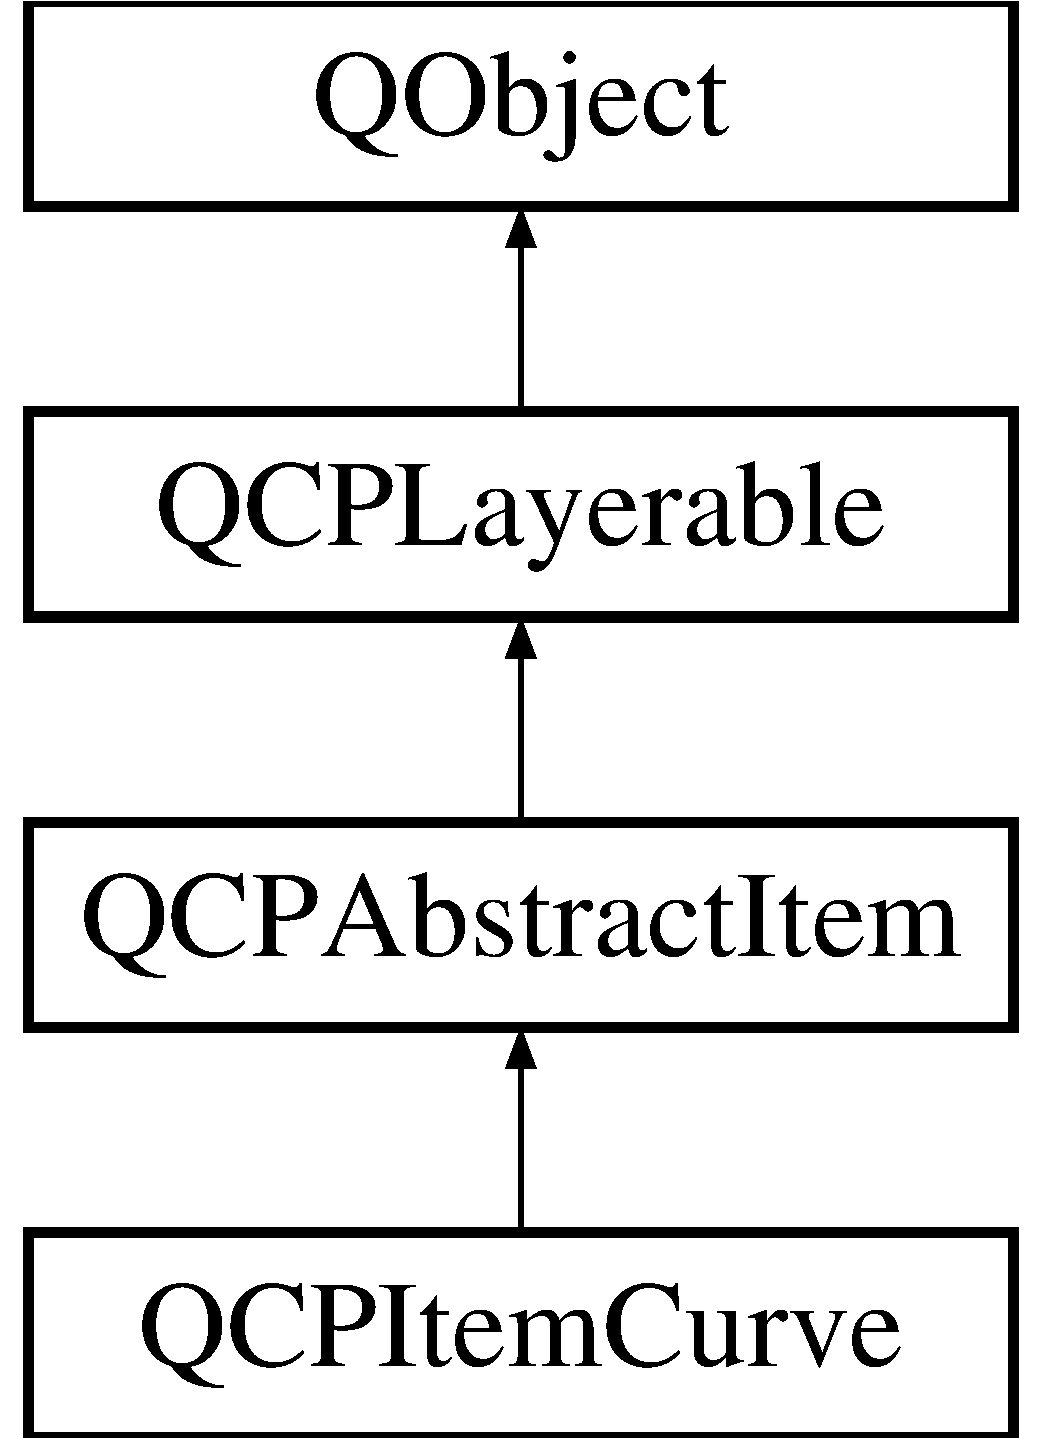
\includegraphics[height=4.000000cm]{class_q_c_p_item_curve}
\end{center}
\end{figure}
\subsection*{Public Member Functions}
\begin{DoxyCompactItemize}
\item 
\hyperlink{class_q_c_p_item_curve_ac9b7508bb5c8827e1a7a6199f8c82bec}{Q\+C\+P\+Item\+Curve} (\hyperlink{class_q_custom_plot}{Q\+Custom\+Plot} $\ast$parent\+Plot)
\item 
\hypertarget{class_q_c_p_item_curve_aefe2e9affaa9c70f434a076def4a7ea5}{}\label{class_q_c_p_item_curve_aefe2e9affaa9c70f434a076def4a7ea5} 
Q\+Pen {\bfseries pen} () const
\item 
\hypertarget{class_q_c_p_item_curve_a4827e5f89e8fb3b2760871c4e5315322}{}\label{class_q_c_p_item_curve_a4827e5f89e8fb3b2760871c4e5315322} 
Q\+Pen {\bfseries selected\+Pen} () const
\item 
\hypertarget{class_q_c_p_item_curve_a86467ff1dc9cbcefead6333bd5e27393}{}\label{class_q_c_p_item_curve_a86467ff1dc9cbcefead6333bd5e27393} 
\hyperlink{class_q_c_p_line_ending}{Q\+C\+P\+Line\+Ending} {\bfseries head} () const
\item 
\hypertarget{class_q_c_p_item_curve_aaef82aa581f6996444028027d6829acc}{}\label{class_q_c_p_item_curve_aaef82aa581f6996444028027d6829acc} 
\hyperlink{class_q_c_p_line_ending}{Q\+C\+P\+Line\+Ending} {\bfseries tail} () const
\item 
void \hyperlink{class_q_c_p_item_curve_a034be908440aec785c34b92843461221}{set\+Pen} (const Q\+Pen \&pen)
\item 
void \hyperlink{class_q_c_p_item_curve_a375b917669f868c5a106bf2f1ab7c26d}{set\+Selected\+Pen} (const Q\+Pen \&pen)
\item 
void \hyperlink{class_q_c_p_item_curve_a08a30d9cdd63995deea3d9e20430676f}{set\+Head} (const \hyperlink{class_q_c_p_line_ending}{Q\+C\+P\+Line\+Ending} \&head)
\item 
void \hyperlink{class_q_c_p_item_curve_ac3488d8b1a6489c845dc5bff3ef71124}{set\+Tail} (const \hyperlink{class_q_c_p_line_ending}{Q\+C\+P\+Line\+Ending} \&tail)
\item 
virtual double \hyperlink{class_q_c_p_item_curve_a8018b8b3fc552a44ba87ca4b64c1523f}{select\+Test} (const Q\+PointF \&pos, bool only\+Selectable, Q\+Variant $\ast$details=0) const
\end{DoxyCompactItemize}
\subsection*{Public Attributes}
\begin{DoxyCompactItemize}
\item 
\hypertarget{class_q_c_p_item_curve_a20c3b5ea31c33764f4f30c2ec7ae518b}{}\label{class_q_c_p_item_curve_a20c3b5ea31c33764f4f30c2ec7ae518b} 
\hyperlink{class_q_c_p_item_position}{Q\+C\+P\+Item\+Position} $\ast$const {\bfseries start}
\item 
\hypertarget{class_q_c_p_item_curve_aa124bf66c09cc51c627fb49db8bf8a7b}{}\label{class_q_c_p_item_curve_aa124bf66c09cc51c627fb49db8bf8a7b} 
\hyperlink{class_q_c_p_item_position}{Q\+C\+P\+Item\+Position} $\ast$const {\bfseries start\+Dir}
\item 
\hypertarget{class_q_c_p_item_curve_a28181a9dee9cc3c3da83a883221bd2d0}{}\label{class_q_c_p_item_curve_a28181a9dee9cc3c3da83a883221bd2d0} 
\hyperlink{class_q_c_p_item_position}{Q\+C\+P\+Item\+Position} $\ast$const {\bfseries end\+Dir}
\item 
\hypertarget{class_q_c_p_item_curve_a24ecbb195b32a08b42b61c2cf08a1b4d}{}\label{class_q_c_p_item_curve_a24ecbb195b32a08b42b61c2cf08a1b4d} 
\hyperlink{class_q_c_p_item_position}{Q\+C\+P\+Item\+Position} $\ast$const {\bfseries end}
\end{DoxyCompactItemize}
\subsection*{Protected Member Functions}
\begin{DoxyCompactItemize}
\item 
\hypertarget{class_q_c_p_item_curve_a56cb5b72cd02db2eda598274a39839a9}{}\label{class_q_c_p_item_curve_a56cb5b72cd02db2eda598274a39839a9} 
virtual void {\bfseries draw} (\hyperlink{class_q_c_p_painter}{Q\+C\+P\+Painter} $\ast$painter)
\item 
\hypertarget{class_q_c_p_item_curve_a3a3a84518e8701211c8c5a40bf3c911f}{}\label{class_q_c_p_item_curve_a3a3a84518e8701211c8c5a40bf3c911f} 
Q\+Pen {\bfseries main\+Pen} () const
\end{DoxyCompactItemize}
\subsection*{Protected Attributes}
\begin{DoxyCompactItemize}
\item 
\hypertarget{class_q_c_p_item_curve_a7ef92988d1db2e4d0311e34c0a57fe42}{}\label{class_q_c_p_item_curve_a7ef92988d1db2e4d0311e34c0a57fe42} 
Q\+Pen {\bfseries m\+Pen}
\item 
\hypertarget{class_q_c_p_item_curve_ab22cbab261b20be5aa8e4ca252149246}{}\label{class_q_c_p_item_curve_ab22cbab261b20be5aa8e4ca252149246} 
Q\+Pen {\bfseries m\+Selected\+Pen}
\item 
\hypertarget{class_q_c_p_item_curve_af2cc26ff199570940dc96f5ec19a13f8}{}\label{class_q_c_p_item_curve_af2cc26ff199570940dc96f5ec19a13f8} 
\hyperlink{class_q_c_p_line_ending}{Q\+C\+P\+Line\+Ending} {\bfseries m\+Head}
\item 
\hypertarget{class_q_c_p_item_curve_af1dca285b97e3f5b892dab827a79f327}{}\label{class_q_c_p_item_curve_af1dca285b97e3f5b892dab827a79f327} 
\hyperlink{class_q_c_p_line_ending}{Q\+C\+P\+Line\+Ending} {\bfseries m\+Tail}
\end{DoxyCompactItemize}
\subsection*{Additional Inherited Members}


\subsection{Detailed Description}
A curved line from one point to another. 

 It has four positions, {\itshape start} and {\itshape end}, which define the end points of the line, and two control points which define the direction the line exits from the start and the direction from which it approaches the end\+: {\itshape start\+Dir} and {\itshape end\+Dir}.

With \hyperlink{class_q_c_p_item_curve_a08a30d9cdd63995deea3d9e20430676f}{set\+Head} and \hyperlink{class_q_c_p_item_curve_ac3488d8b1a6489c845dc5bff3ef71124}{set\+Tail} you may set different line ending styles, e.\+g. to create an arrow.

Often it is desirable for the control points to stay at fixed relative positions to the start/end point. This can be achieved by setting the parent anchor e.\+g. of {\itshape start\+Dir} simply to {\itshape start}, and then specify the desired pixel offset with \hyperlink{class_q_c_p_item_position_aa988ba4e87ab684c9021017dcaba945f}{Q\+C\+P\+Item\+Position\+::set\+Coords} on {\itshape start\+Dir}. 

\subsection{Constructor \& Destructor Documentation}
\hypertarget{class_q_c_p_item_curve_ac9b7508bb5c8827e1a7a6199f8c82bec}{}\label{class_q_c_p_item_curve_ac9b7508bb5c8827e1a7a6199f8c82bec} 
\index{Q\+C\+P\+Item\+Curve@{Q\+C\+P\+Item\+Curve}!Q\+C\+P\+Item\+Curve@{Q\+C\+P\+Item\+Curve}}
\index{Q\+C\+P\+Item\+Curve@{Q\+C\+P\+Item\+Curve}!Q\+C\+P\+Item\+Curve@{Q\+C\+P\+Item\+Curve}}
\subsubsection{\texorpdfstring{Q\+C\+P\+Item\+Curve()}{QCPItemCurve()}}
{\footnotesize\ttfamily Q\+C\+P\+Item\+Curve\+::\+Q\+C\+P\+Item\+Curve (\begin{DoxyParamCaption}\item[{\hyperlink{class_q_custom_plot}{Q\+Custom\+Plot} $\ast$}]{parent\+Plot }\end{DoxyParamCaption})}

Creates a curve item and sets default values.

The constructed item can be added to the plot with \hyperlink{class_q_custom_plot_aa500620379262321685cb7a7674cbd2a}{Q\+Custom\+Plot\+::add\+Item}. 

\subsection{Member Function Documentation}
\hypertarget{class_q_c_p_item_curve_a8018b8b3fc552a44ba87ca4b64c1523f}{}\label{class_q_c_p_item_curve_a8018b8b3fc552a44ba87ca4b64c1523f} 
\index{Q\+C\+P\+Item\+Curve@{Q\+C\+P\+Item\+Curve}!select\+Test@{select\+Test}}
\index{select\+Test@{select\+Test}!Q\+C\+P\+Item\+Curve@{Q\+C\+P\+Item\+Curve}}
\subsubsection{\texorpdfstring{select\+Test()}{selectTest()}}
{\footnotesize\ttfamily double Q\+C\+P\+Item\+Curve\+::select\+Test (\begin{DoxyParamCaption}\item[{const Q\+PointF \&}]{pos,  }\item[{bool}]{only\+Selectable,  }\item[{Q\+Variant $\ast$}]{details = {\ttfamily 0} }\end{DoxyParamCaption}) const\hspace{0.3cm}{\ttfamily [virtual]}}

This function is used to decide whether a click hits a layerable object or not.

{\itshape pos} is a point in pixel coordinates on the \hyperlink{class_q_custom_plot}{Q\+Custom\+Plot} surface. This function returns the shortest pixel distance of this point to the object. If the object is either invisible or the distance couldn\textquotesingle{}t be determined, -\/1.\+0 is returned. Further, if {\itshape only\+Selectable} is true and the object is not selectable, -\/1.\+0 is returned, too.

If the object is represented not by single lines but by an area like a \hyperlink{class_q_c_p_item_text}{Q\+C\+P\+Item\+Text} or the bars of a \hyperlink{class_q_c_p_bars}{Q\+C\+P\+Bars} plottable, a click inside the area should also be considered a hit. In these cases this function thus returns a constant value greater zero but still below the parent plot\textquotesingle{}s selection tolerance. (typically the selection\+Tolerance multiplied by 0.\+99).

Providing a constant value for area objects allows selecting line objects even when they are obscured by such area objects, by clicking close to the lines (i.\+e. closer than 0.\+99$\ast$selection\+Tolerance).

The actual setting of the selection state is not done by this function. This is handled by the parent \hyperlink{class_q_custom_plot}{Q\+Custom\+Plot} when the mouse\+Release\+Event occurs, and the finally selected object is notified via the select\+Event/deselect\+Event methods.

{\itshape details} is an optional output parameter. Every layerable subclass may place any information in {\itshape details}. This information will be passed to select\+Event when the parent \hyperlink{class_q_custom_plot}{Q\+Custom\+Plot} decides on the basis of this select\+Test call, that the object was successfully selected. The subsequent call to select\+Event will carry the {\itshape details}. This is useful for multi-\/part objects (like \hyperlink{class_q_c_p_axis}{Q\+C\+P\+Axis}). This way, a possibly complex calculation to decide which part was clicked is only done once in \hyperlink{class_q_c_p_item_curve_a8018b8b3fc552a44ba87ca4b64c1523f}{select\+Test}. The result (i.\+e. the actually clicked part) can then be placed in {\itshape details}. So in the subsequent select\+Event, the decision which part was selected doesn\textquotesingle{}t have to be done a second time for a single selection operation.

You may pass 0 as {\itshape details} to indicate that you are not interested in those selection details.

\begin{DoxySeeAlso}{See also}
select\+Event, deselect\+Event, \hyperlink{class_q_custom_plot_a5ee1e2f6ae27419deca53e75907c27e5}{Q\+Custom\+Plot\+::set\+Interactions} 
\end{DoxySeeAlso}


Implements \hyperlink{class_q_c_p_abstract_item_a96d522d10ffc0413b9a366c6f7f0476b}{Q\+C\+P\+Abstract\+Item}.

\hypertarget{class_q_c_p_item_curve_a08a30d9cdd63995deea3d9e20430676f}{}\label{class_q_c_p_item_curve_a08a30d9cdd63995deea3d9e20430676f} 
\index{Q\+C\+P\+Item\+Curve@{Q\+C\+P\+Item\+Curve}!set\+Head@{set\+Head}}
\index{set\+Head@{set\+Head}!Q\+C\+P\+Item\+Curve@{Q\+C\+P\+Item\+Curve}}
\subsubsection{\texorpdfstring{set\+Head()}{setHead()}}
{\footnotesize\ttfamily void Q\+C\+P\+Item\+Curve\+::set\+Head (\begin{DoxyParamCaption}\item[{const \hyperlink{class_q_c_p_line_ending}{Q\+C\+P\+Line\+Ending} \&}]{head }\end{DoxyParamCaption})}

Sets the line ending style of the head. The head corresponds to the {\itshape end} position.

Note that due to the overloaded \hyperlink{class_q_c_p_line_ending}{Q\+C\+P\+Line\+Ending} constructor, you may directly specify a \hyperlink{class_q_c_p_line_ending_a5ef16e6876b4b74959c7261d8d4c2cd5}{Q\+C\+P\+Line\+Ending\+::\+Ending\+Style} here, e.\+g.
\begin{DoxyCode}
\hyperlink{class_q_c_p_item_curve_a08a30d9cdd63995deea3d9e20430676f}{setHead}(\hyperlink{class_q_c_p_line_ending_a5ef16e6876b4b74959c7261d8d4c2cd5ab9964d0d03f812d1e79de15edbeb2cbf}{QCPLineEnding::esSpikeArrow}) 
\end{DoxyCode}


\begin{DoxySeeAlso}{See also}
\hyperlink{class_q_c_p_item_curve_ac3488d8b1a6489c845dc5bff3ef71124}{set\+Tail} 
\end{DoxySeeAlso}
\hypertarget{class_q_c_p_item_curve_a034be908440aec785c34b92843461221}{}\label{class_q_c_p_item_curve_a034be908440aec785c34b92843461221} 
\index{Q\+C\+P\+Item\+Curve@{Q\+C\+P\+Item\+Curve}!set\+Pen@{set\+Pen}}
\index{set\+Pen@{set\+Pen}!Q\+C\+P\+Item\+Curve@{Q\+C\+P\+Item\+Curve}}
\subsubsection{\texorpdfstring{set\+Pen()}{setPen()}}
{\footnotesize\ttfamily void Q\+C\+P\+Item\+Curve\+::set\+Pen (\begin{DoxyParamCaption}\item[{const Q\+Pen \&}]{pen }\end{DoxyParamCaption})}

Sets the pen that will be used to draw the line

\begin{DoxySeeAlso}{See also}
\hyperlink{class_q_c_p_item_curve_a375b917669f868c5a106bf2f1ab7c26d}{set\+Selected\+Pen} 
\end{DoxySeeAlso}
\hypertarget{class_q_c_p_item_curve_a375b917669f868c5a106bf2f1ab7c26d}{}\label{class_q_c_p_item_curve_a375b917669f868c5a106bf2f1ab7c26d} 
\index{Q\+C\+P\+Item\+Curve@{Q\+C\+P\+Item\+Curve}!set\+Selected\+Pen@{set\+Selected\+Pen}}
\index{set\+Selected\+Pen@{set\+Selected\+Pen}!Q\+C\+P\+Item\+Curve@{Q\+C\+P\+Item\+Curve}}
\subsubsection{\texorpdfstring{set\+Selected\+Pen()}{setSelectedPen()}}
{\footnotesize\ttfamily void Q\+C\+P\+Item\+Curve\+::set\+Selected\+Pen (\begin{DoxyParamCaption}\item[{const Q\+Pen \&}]{pen }\end{DoxyParamCaption})}

Sets the pen that will be used to draw the line when selected

\begin{DoxySeeAlso}{See also}
\hyperlink{class_q_c_p_item_curve_a034be908440aec785c34b92843461221}{set\+Pen}, \hyperlink{class_q_c_p_abstract_item_a203de94ad586cc44d16c9565f49d3378}{set\+Selected} 
\end{DoxySeeAlso}
\hypertarget{class_q_c_p_item_curve_ac3488d8b1a6489c845dc5bff3ef71124}{}\label{class_q_c_p_item_curve_ac3488d8b1a6489c845dc5bff3ef71124} 
\index{Q\+C\+P\+Item\+Curve@{Q\+C\+P\+Item\+Curve}!set\+Tail@{set\+Tail}}
\index{set\+Tail@{set\+Tail}!Q\+C\+P\+Item\+Curve@{Q\+C\+P\+Item\+Curve}}
\subsubsection{\texorpdfstring{set\+Tail()}{setTail()}}
{\footnotesize\ttfamily void Q\+C\+P\+Item\+Curve\+::set\+Tail (\begin{DoxyParamCaption}\item[{const \hyperlink{class_q_c_p_line_ending}{Q\+C\+P\+Line\+Ending} \&}]{tail }\end{DoxyParamCaption})}

Sets the line ending style of the tail. The tail corresponds to the {\itshape start} position.

Note that due to the overloaded \hyperlink{class_q_c_p_line_ending}{Q\+C\+P\+Line\+Ending} constructor, you may directly specify a \hyperlink{class_q_c_p_line_ending_a5ef16e6876b4b74959c7261d8d4c2cd5}{Q\+C\+P\+Line\+Ending\+::\+Ending\+Style} here, e.\+g.
\begin{DoxyCode}
\hyperlink{class_q_c_p_item_curve_ac3488d8b1a6489c845dc5bff3ef71124}{setTail}(\hyperlink{class_q_c_p_line_ending_a5ef16e6876b4b74959c7261d8d4c2cd5ab9964d0d03f812d1e79de15edbeb2cbf}{QCPLineEnding::esSpikeArrow}) 
\end{DoxyCode}


\begin{DoxySeeAlso}{See also}
\hyperlink{class_q_c_p_item_curve_a08a30d9cdd63995deea3d9e20430676f}{set\+Head} 
\end{DoxySeeAlso}


The documentation for this class was generated from the following files\+:\begin{DoxyCompactItemize}
\item 
F\+E\+S\+S-\/\+G\+U\+I/\hyperlink{qcustomplot_8h}{qcustomplot.\+h}\item 
F\+E\+S\+S-\/\+G\+U\+I/\hyperlink{qcustomplot_8cpp}{qcustomplot.\+cpp}\end{DoxyCompactItemize}

\hypertarget{class_q_c_p_item_ellipse}{}\section{Q\+C\+P\+Item\+Ellipse Class Reference}
\label{class_q_c_p_item_ellipse}\index{Q\+C\+P\+Item\+Ellipse@{Q\+C\+P\+Item\+Ellipse}}


An ellipse.  


Inheritance diagram for Q\+C\+P\+Item\+Ellipse\+:\begin{figure}[H]
\begin{center}
\leavevmode
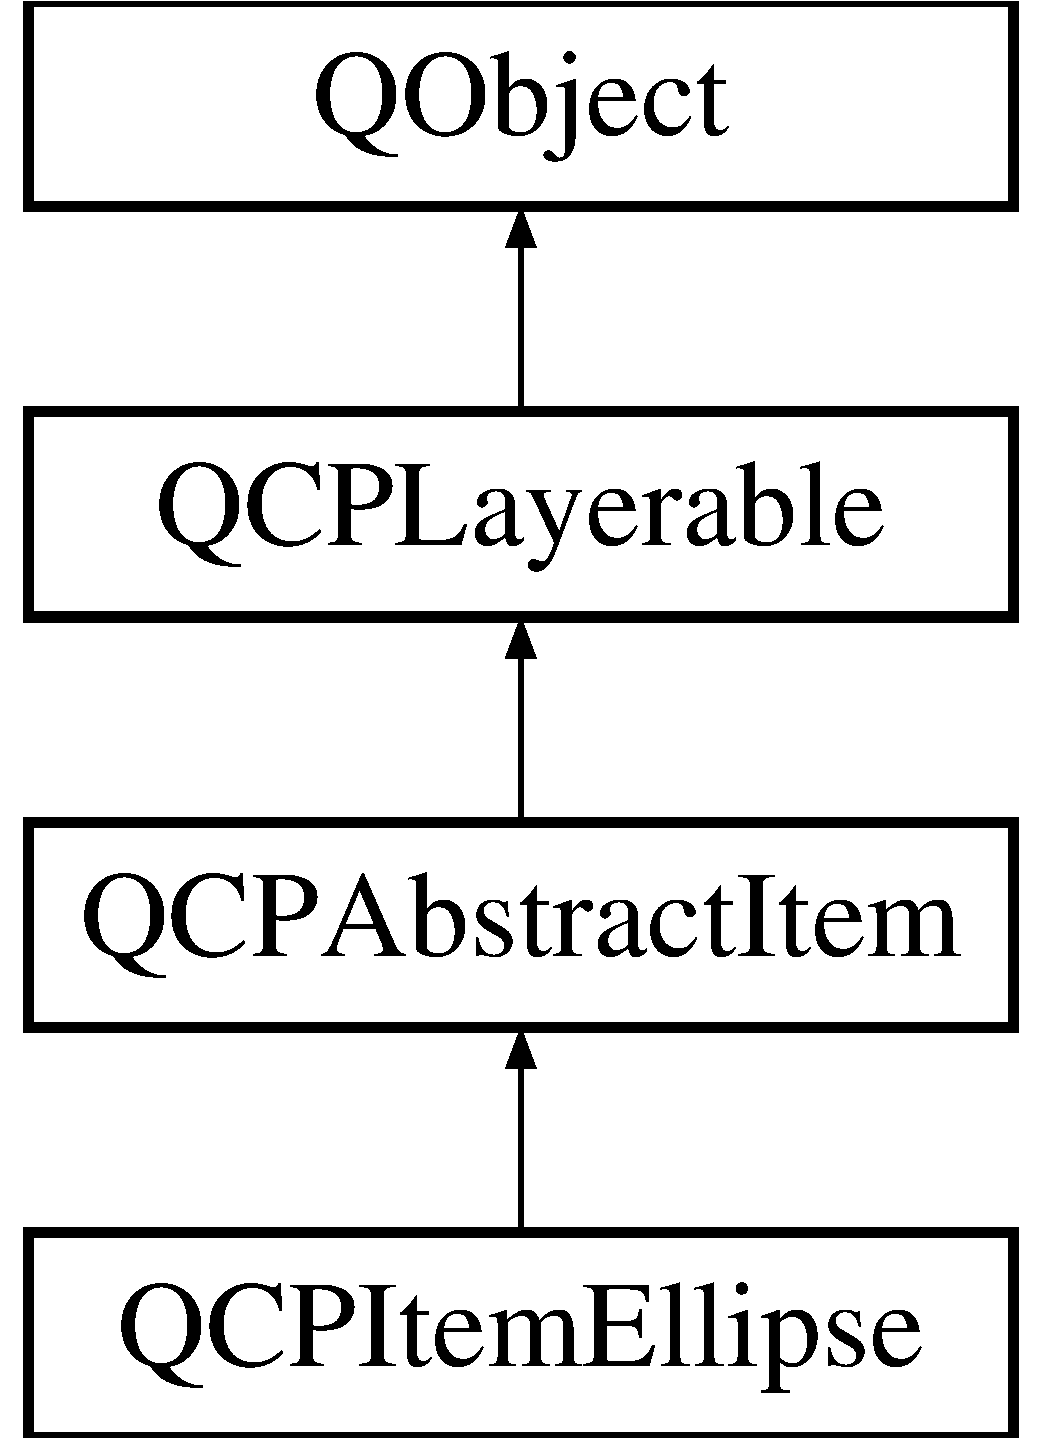
\includegraphics[height=4.000000cm]{class_q_c_p_item_ellipse}
\end{center}
\end{figure}
\subsection*{Public Member Functions}
\begin{DoxyCompactItemize}
\item 
\hyperlink{class_q_c_p_item_ellipse_a759b77ef002515eba0263b5447ecb3fb}{Q\+C\+P\+Item\+Ellipse} (\hyperlink{class_q_custom_plot}{Q\+Custom\+Plot} $\ast$parent\+Plot)
\item 
\hypertarget{class_q_c_p_item_ellipse_a8288f7ce760fc795f5ce4e61136bda19}{}\label{class_q_c_p_item_ellipse_a8288f7ce760fc795f5ce4e61136bda19} 
Q\+Pen {\bfseries pen} () const
\item 
\hypertarget{class_q_c_p_item_ellipse_a9a200af2797356b45479b601d75437ee}{}\label{class_q_c_p_item_ellipse_a9a200af2797356b45479b601d75437ee} 
Q\+Pen {\bfseries selected\+Pen} () const
\item 
\hypertarget{class_q_c_p_item_ellipse_aacf45d032f204d0df3dd0bfdf1172cd3}{}\label{class_q_c_p_item_ellipse_aacf45d032f204d0df3dd0bfdf1172cd3} 
Q\+Brush {\bfseries brush} () const
\item 
\hypertarget{class_q_c_p_item_ellipse_afeda9d8e2e6da216a3c3366d87e80feb}{}\label{class_q_c_p_item_ellipse_afeda9d8e2e6da216a3c3366d87e80feb} 
Q\+Brush {\bfseries selected\+Brush} () const
\item 
void \hyperlink{class_q_c_p_item_ellipse_adb81a663ed2420fcfa011e49f678d1a6}{set\+Pen} (const Q\+Pen \&pen)
\item 
void \hyperlink{class_q_c_p_item_ellipse_a6c542fba1dc918041c583f58a50dde99}{set\+Selected\+Pen} (const Q\+Pen \&pen)
\item 
void \hyperlink{class_q_c_p_item_ellipse_a49fc74e6965834e873d027d026def798}{set\+Brush} (const Q\+Brush \&brush)
\item 
void \hyperlink{class_q_c_p_item_ellipse_a9693501cfaa43a099655c75bed0dab3f}{set\+Selected\+Brush} (const Q\+Brush \&brush)
\item 
virtual double \hyperlink{class_q_c_p_item_ellipse_aa41be2180b2ace2e303b88d005c14243}{select\+Test} (const Q\+PointF \&pos, bool only\+Selectable, Q\+Variant $\ast$details=0) const
\end{DoxyCompactItemize}
\subsection*{Public Attributes}
\begin{DoxyCompactItemize}
\item 
\hypertarget{class_q_c_p_item_ellipse_a12fd8420c06718d0c8a2303d6a652848}{}\label{class_q_c_p_item_ellipse_a12fd8420c06718d0c8a2303d6a652848} 
\hyperlink{class_q_c_p_item_position}{Q\+C\+P\+Item\+Position} $\ast$const {\bfseries top\+Left}
\item 
\hypertarget{class_q_c_p_item_ellipse_ab73c8deafc0d8d1ef7d75b6cdcc37159}{}\label{class_q_c_p_item_ellipse_ab73c8deafc0d8d1ef7d75b6cdcc37159} 
\hyperlink{class_q_c_p_item_position}{Q\+C\+P\+Item\+Position} $\ast$const {\bfseries bottom\+Right}
\item 
\hypertarget{class_q_c_p_item_ellipse_a33ebd2a751b63b9240edc9aa46c19eff}{}\label{class_q_c_p_item_ellipse_a33ebd2a751b63b9240edc9aa46c19eff} 
\hyperlink{class_q_c_p_item_anchor}{Q\+C\+P\+Item\+Anchor} $\ast$const {\bfseries top\+Left\+Rim}
\item 
\hypertarget{class_q_c_p_item_ellipse_ad50f907d6f9d1402c6c5d302dca5c5d5}{}\label{class_q_c_p_item_ellipse_ad50f907d6f9d1402c6c5d302dca5c5d5} 
\hyperlink{class_q_c_p_item_anchor}{Q\+C\+P\+Item\+Anchor} $\ast$const {\bfseries top}
\item 
\hypertarget{class_q_c_p_item_ellipse_a744446970b38a4a3bbea46d722b7c54d}{}\label{class_q_c_p_item_ellipse_a744446970b38a4a3bbea46d722b7c54d} 
\hyperlink{class_q_c_p_item_anchor}{Q\+C\+P\+Item\+Anchor} $\ast$const {\bfseries top\+Right\+Rim}
\item 
\hypertarget{class_q_c_p_item_ellipse_a50091a3bd8761d3ce0d95d9c727e4a82}{}\label{class_q_c_p_item_ellipse_a50091a3bd8761d3ce0d95d9c727e4a82} 
\hyperlink{class_q_c_p_item_anchor}{Q\+C\+P\+Item\+Anchor} $\ast$const {\bfseries right}
\item 
\hypertarget{class_q_c_p_item_ellipse_a5c8404be601d61b7fafeaaf1c05c4c42}{}\label{class_q_c_p_item_ellipse_a5c8404be601d61b7fafeaaf1c05c4c42} 
\hyperlink{class_q_c_p_item_anchor}{Q\+C\+P\+Item\+Anchor} $\ast$const {\bfseries bottom\+Right\+Rim}
\item 
\hypertarget{class_q_c_p_item_ellipse_a2dc80ff9f5db600eae0133bdde65066f}{}\label{class_q_c_p_item_ellipse_a2dc80ff9f5db600eae0133bdde65066f} 
\hyperlink{class_q_c_p_item_anchor}{Q\+C\+P\+Item\+Anchor} $\ast$const {\bfseries bottom}
\item 
\hypertarget{class_q_c_p_item_ellipse_a31f31a9e9f9098c90fb47573094276c5}{}\label{class_q_c_p_item_ellipse_a31f31a9e9f9098c90fb47573094276c5} 
\hyperlink{class_q_c_p_item_anchor}{Q\+C\+P\+Item\+Anchor} $\ast$const {\bfseries bottom\+Left\+Rim}
\item 
\hypertarget{class_q_c_p_item_ellipse_aa259cd03efaedf60cf5b1019b20e4f2b}{}\label{class_q_c_p_item_ellipse_aa259cd03efaedf60cf5b1019b20e4f2b} 
\hyperlink{class_q_c_p_item_anchor}{Q\+C\+P\+Item\+Anchor} $\ast$const {\bfseries left}
\item 
\hypertarget{class_q_c_p_item_ellipse_a8b6dd0e854f99239c5806ffdf2f590b3}{}\label{class_q_c_p_item_ellipse_a8b6dd0e854f99239c5806ffdf2f590b3} 
\hyperlink{class_q_c_p_item_anchor}{Q\+C\+P\+Item\+Anchor} $\ast$const {\bfseries center}
\end{DoxyCompactItemize}
\subsection*{Protected Types}
\begin{DoxyCompactItemize}
\item 
\hypertarget{class_q_c_p_item_ellipse_a415009889543169f35b70795f415e45e}{}\label{class_q_c_p_item_ellipse_a415009889543169f35b70795f415e45e} 
enum {\bfseries Anchor\+Index} \{ \newline
{\bfseries ai\+Top\+Left\+Rim}, 
{\bfseries ai\+Top}, 
{\bfseries ai\+Top\+Right\+Rim}, 
{\bfseries ai\+Right}, 
\newline
{\bfseries ai\+Bottom\+Right\+Rim}, 
{\bfseries ai\+Bottom}, 
{\bfseries ai\+Bottom\+Left\+Rim}, 
{\bfseries ai\+Left}, 
\newline
{\bfseries ai\+Center}
 \}
\end{DoxyCompactItemize}
\subsection*{Protected Member Functions}
\begin{DoxyCompactItemize}
\item 
\hypertarget{class_q_c_p_item_ellipse_afe97ec827adb05f000fe007783faae3c}{}\label{class_q_c_p_item_ellipse_afe97ec827adb05f000fe007783faae3c} 
virtual void {\bfseries draw} (\hyperlink{class_q_c_p_painter}{Q\+C\+P\+Painter} $\ast$painter)
\item 
\hypertarget{class_q_c_p_item_ellipse_ac9de21db25a5b93594ee540533a4e7e4}{}\label{class_q_c_p_item_ellipse_ac9de21db25a5b93594ee540533a4e7e4} 
virtual Q\+PointF {\bfseries anchor\+Pixel\+Point} (int anchor\+Id) const
\item 
\hypertarget{class_q_c_p_item_ellipse_a9c11717026dfd685c83a9650666b7181}{}\label{class_q_c_p_item_ellipse_a9c11717026dfd685c83a9650666b7181} 
Q\+Pen {\bfseries main\+Pen} () const
\item 
\hypertarget{class_q_c_p_item_ellipse_a6218bdf5e703f609b934b0bf9c8d0971}{}\label{class_q_c_p_item_ellipse_a6218bdf5e703f609b934b0bf9c8d0971} 
Q\+Brush {\bfseries main\+Brush} () const
\end{DoxyCompactItemize}
\subsection*{Protected Attributes}
\begin{DoxyCompactItemize}
\item 
\hypertarget{class_q_c_p_item_ellipse_a16ad9389acf028a7e4ac8fd7a550b2e4}{}\label{class_q_c_p_item_ellipse_a16ad9389acf028a7e4ac8fd7a550b2e4} 
Q\+Pen {\bfseries m\+Pen}
\item 
\hypertarget{class_q_c_p_item_ellipse_a57b047abfce6f1a84ed46ca668c90e21}{}\label{class_q_c_p_item_ellipse_a57b047abfce6f1a84ed46ca668c90e21} 
Q\+Pen {\bfseries m\+Selected\+Pen}
\item 
\hypertarget{class_q_c_p_item_ellipse_a6fa59478cd3ad1b10e6c1f6cedc84bd6}{}\label{class_q_c_p_item_ellipse_a6fa59478cd3ad1b10e6c1f6cedc84bd6} 
Q\+Brush {\bfseries m\+Brush}
\item 
\hypertarget{class_q_c_p_item_ellipse_a2e49d5547478aa36910ed8a2dcc8a5c0}{}\label{class_q_c_p_item_ellipse_a2e49d5547478aa36910ed8a2dcc8a5c0} 
Q\+Brush {\bfseries m\+Selected\+Brush}
\end{DoxyCompactItemize}
\subsection*{Additional Inherited Members}


\subsection{Detailed Description}
An ellipse. 

 It has two positions, {\itshape top\+Left} and {\itshape bottom\+Right}, which define the rect the ellipse will be drawn in. 

\subsection{Constructor \& Destructor Documentation}
\hypertarget{class_q_c_p_item_ellipse_a759b77ef002515eba0263b5447ecb3fb}{}\label{class_q_c_p_item_ellipse_a759b77ef002515eba0263b5447ecb3fb} 
\index{Q\+C\+P\+Item\+Ellipse@{Q\+C\+P\+Item\+Ellipse}!Q\+C\+P\+Item\+Ellipse@{Q\+C\+P\+Item\+Ellipse}}
\index{Q\+C\+P\+Item\+Ellipse@{Q\+C\+P\+Item\+Ellipse}!Q\+C\+P\+Item\+Ellipse@{Q\+C\+P\+Item\+Ellipse}}
\subsubsection{\texorpdfstring{Q\+C\+P\+Item\+Ellipse()}{QCPItemEllipse()}}
{\footnotesize\ttfamily Q\+C\+P\+Item\+Ellipse\+::\+Q\+C\+P\+Item\+Ellipse (\begin{DoxyParamCaption}\item[{\hyperlink{class_q_custom_plot}{Q\+Custom\+Plot} $\ast$}]{parent\+Plot }\end{DoxyParamCaption})}

Creates an ellipse item and sets default values.

The constructed item can be added to the plot with \hyperlink{class_q_custom_plot_aa500620379262321685cb7a7674cbd2a}{Q\+Custom\+Plot\+::add\+Item}. 

\subsection{Member Function Documentation}
\hypertarget{class_q_c_p_item_ellipse_aa41be2180b2ace2e303b88d005c14243}{}\label{class_q_c_p_item_ellipse_aa41be2180b2ace2e303b88d005c14243} 
\index{Q\+C\+P\+Item\+Ellipse@{Q\+C\+P\+Item\+Ellipse}!select\+Test@{select\+Test}}
\index{select\+Test@{select\+Test}!Q\+C\+P\+Item\+Ellipse@{Q\+C\+P\+Item\+Ellipse}}
\subsubsection{\texorpdfstring{select\+Test()}{selectTest()}}
{\footnotesize\ttfamily double Q\+C\+P\+Item\+Ellipse\+::select\+Test (\begin{DoxyParamCaption}\item[{const Q\+PointF \&}]{pos,  }\item[{bool}]{only\+Selectable,  }\item[{Q\+Variant $\ast$}]{details = {\ttfamily 0} }\end{DoxyParamCaption}) const\hspace{0.3cm}{\ttfamily [virtual]}}

This function is used to decide whether a click hits a layerable object or not.

{\itshape pos} is a point in pixel coordinates on the \hyperlink{class_q_custom_plot}{Q\+Custom\+Plot} surface. This function returns the shortest pixel distance of this point to the object. If the object is either invisible or the distance couldn\textquotesingle{}t be determined, -\/1.\+0 is returned. Further, if {\itshape only\+Selectable} is true and the object is not selectable, -\/1.\+0 is returned, too.

If the object is represented not by single lines but by an area like a \hyperlink{class_q_c_p_item_text}{Q\+C\+P\+Item\+Text} or the bars of a \hyperlink{class_q_c_p_bars}{Q\+C\+P\+Bars} plottable, a click inside the area should also be considered a hit. In these cases this function thus returns a constant value greater zero but still below the parent plot\textquotesingle{}s selection tolerance. (typically the selection\+Tolerance multiplied by 0.\+99).

Providing a constant value for area objects allows selecting line objects even when they are obscured by such area objects, by clicking close to the lines (i.\+e. closer than 0.\+99$\ast$selection\+Tolerance).

The actual setting of the selection state is not done by this function. This is handled by the parent \hyperlink{class_q_custom_plot}{Q\+Custom\+Plot} when the mouse\+Release\+Event occurs, and the finally selected object is notified via the select\+Event/deselect\+Event methods.

{\itshape details} is an optional output parameter. Every layerable subclass may place any information in {\itshape details}. This information will be passed to select\+Event when the parent \hyperlink{class_q_custom_plot}{Q\+Custom\+Plot} decides on the basis of this select\+Test call, that the object was successfully selected. The subsequent call to select\+Event will carry the {\itshape details}. This is useful for multi-\/part objects (like \hyperlink{class_q_c_p_axis}{Q\+C\+P\+Axis}). This way, a possibly complex calculation to decide which part was clicked is only done once in \hyperlink{class_q_c_p_item_ellipse_aa41be2180b2ace2e303b88d005c14243}{select\+Test}. The result (i.\+e. the actually clicked part) can then be placed in {\itshape details}. So in the subsequent select\+Event, the decision which part was selected doesn\textquotesingle{}t have to be done a second time for a single selection operation.

You may pass 0 as {\itshape details} to indicate that you are not interested in those selection details.

\begin{DoxySeeAlso}{See also}
select\+Event, deselect\+Event, \hyperlink{class_q_custom_plot_a5ee1e2f6ae27419deca53e75907c27e5}{Q\+Custom\+Plot\+::set\+Interactions} 
\end{DoxySeeAlso}


Implements \hyperlink{class_q_c_p_abstract_item_a96d522d10ffc0413b9a366c6f7f0476b}{Q\+C\+P\+Abstract\+Item}.

\hypertarget{class_q_c_p_item_ellipse_a49fc74e6965834e873d027d026def798}{}\label{class_q_c_p_item_ellipse_a49fc74e6965834e873d027d026def798} 
\index{Q\+C\+P\+Item\+Ellipse@{Q\+C\+P\+Item\+Ellipse}!set\+Brush@{set\+Brush}}
\index{set\+Brush@{set\+Brush}!Q\+C\+P\+Item\+Ellipse@{Q\+C\+P\+Item\+Ellipse}}
\subsubsection{\texorpdfstring{set\+Brush()}{setBrush()}}
{\footnotesize\ttfamily void Q\+C\+P\+Item\+Ellipse\+::set\+Brush (\begin{DoxyParamCaption}\item[{const Q\+Brush \&}]{brush }\end{DoxyParamCaption})}

Sets the brush that will be used to fill the ellipse. To disable filling, set {\itshape brush} to Qt\+::\+No\+Brush.

\begin{DoxySeeAlso}{See also}
\hyperlink{class_q_c_p_item_ellipse_a9693501cfaa43a099655c75bed0dab3f}{set\+Selected\+Brush}, \hyperlink{class_q_c_p_item_ellipse_adb81a663ed2420fcfa011e49f678d1a6}{set\+Pen} 
\end{DoxySeeAlso}
\hypertarget{class_q_c_p_item_ellipse_adb81a663ed2420fcfa011e49f678d1a6}{}\label{class_q_c_p_item_ellipse_adb81a663ed2420fcfa011e49f678d1a6} 
\index{Q\+C\+P\+Item\+Ellipse@{Q\+C\+P\+Item\+Ellipse}!set\+Pen@{set\+Pen}}
\index{set\+Pen@{set\+Pen}!Q\+C\+P\+Item\+Ellipse@{Q\+C\+P\+Item\+Ellipse}}
\subsubsection{\texorpdfstring{set\+Pen()}{setPen()}}
{\footnotesize\ttfamily void Q\+C\+P\+Item\+Ellipse\+::set\+Pen (\begin{DoxyParamCaption}\item[{const Q\+Pen \&}]{pen }\end{DoxyParamCaption})}

Sets the pen that will be used to draw the line of the ellipse

\begin{DoxySeeAlso}{See also}
\hyperlink{class_q_c_p_item_ellipse_a6c542fba1dc918041c583f58a50dde99}{set\+Selected\+Pen}, \hyperlink{class_q_c_p_item_ellipse_a49fc74e6965834e873d027d026def798}{set\+Brush} 
\end{DoxySeeAlso}
\hypertarget{class_q_c_p_item_ellipse_a9693501cfaa43a099655c75bed0dab3f}{}\label{class_q_c_p_item_ellipse_a9693501cfaa43a099655c75bed0dab3f} 
\index{Q\+C\+P\+Item\+Ellipse@{Q\+C\+P\+Item\+Ellipse}!set\+Selected\+Brush@{set\+Selected\+Brush}}
\index{set\+Selected\+Brush@{set\+Selected\+Brush}!Q\+C\+P\+Item\+Ellipse@{Q\+C\+P\+Item\+Ellipse}}
\subsubsection{\texorpdfstring{set\+Selected\+Brush()}{setSelectedBrush()}}
{\footnotesize\ttfamily void Q\+C\+P\+Item\+Ellipse\+::set\+Selected\+Brush (\begin{DoxyParamCaption}\item[{const Q\+Brush \&}]{brush }\end{DoxyParamCaption})}

Sets the brush that will be used to fill the ellipse when selected. To disable filling, set {\itshape brush} to Qt\+::\+No\+Brush.

\begin{DoxySeeAlso}{See also}
\hyperlink{class_q_c_p_item_ellipse_a49fc74e6965834e873d027d026def798}{set\+Brush} 
\end{DoxySeeAlso}
\hypertarget{class_q_c_p_item_ellipse_a6c542fba1dc918041c583f58a50dde99}{}\label{class_q_c_p_item_ellipse_a6c542fba1dc918041c583f58a50dde99} 
\index{Q\+C\+P\+Item\+Ellipse@{Q\+C\+P\+Item\+Ellipse}!set\+Selected\+Pen@{set\+Selected\+Pen}}
\index{set\+Selected\+Pen@{set\+Selected\+Pen}!Q\+C\+P\+Item\+Ellipse@{Q\+C\+P\+Item\+Ellipse}}
\subsubsection{\texorpdfstring{set\+Selected\+Pen()}{setSelectedPen()}}
{\footnotesize\ttfamily void Q\+C\+P\+Item\+Ellipse\+::set\+Selected\+Pen (\begin{DoxyParamCaption}\item[{const Q\+Pen \&}]{pen }\end{DoxyParamCaption})}

Sets the pen that will be used to draw the line of the ellipse when selected

\begin{DoxySeeAlso}{See also}
\hyperlink{class_q_c_p_item_ellipse_adb81a663ed2420fcfa011e49f678d1a6}{set\+Pen}, \hyperlink{class_q_c_p_abstract_item_a203de94ad586cc44d16c9565f49d3378}{set\+Selected} 
\end{DoxySeeAlso}


The documentation for this class was generated from the following files\+:\begin{DoxyCompactItemize}
\item 
C\+:/\+Users/\+Jesse Jutson/\+Documents/\+Git\+Hub/\+F\+E\+S\+S\+G\+U\+I/\+F\+E\+S\+S-\/\+G\+U\+I/\hyperlink{qcustomplot_8h}{qcustomplot.\+h}\item 
C\+:/\+Users/\+Jesse Jutson/\+Documents/\+Git\+Hub/\+F\+E\+S\+S\+G\+U\+I/\+F\+E\+S\+S-\/\+G\+U\+I/\hyperlink{qcustomplot_8cpp}{qcustomplot.\+cpp}\end{DoxyCompactItemize}

\hypertarget{class_q_c_p_item_line}{}\section{Q\+C\+P\+Item\+Line Class Reference}
\label{class_q_c_p_item_line}\index{Q\+C\+P\+Item\+Line@{Q\+C\+P\+Item\+Line}}


A line from one point to another.  


Inheritance diagram for Q\+C\+P\+Item\+Line\+:\begin{figure}[H]
\begin{center}
\leavevmode
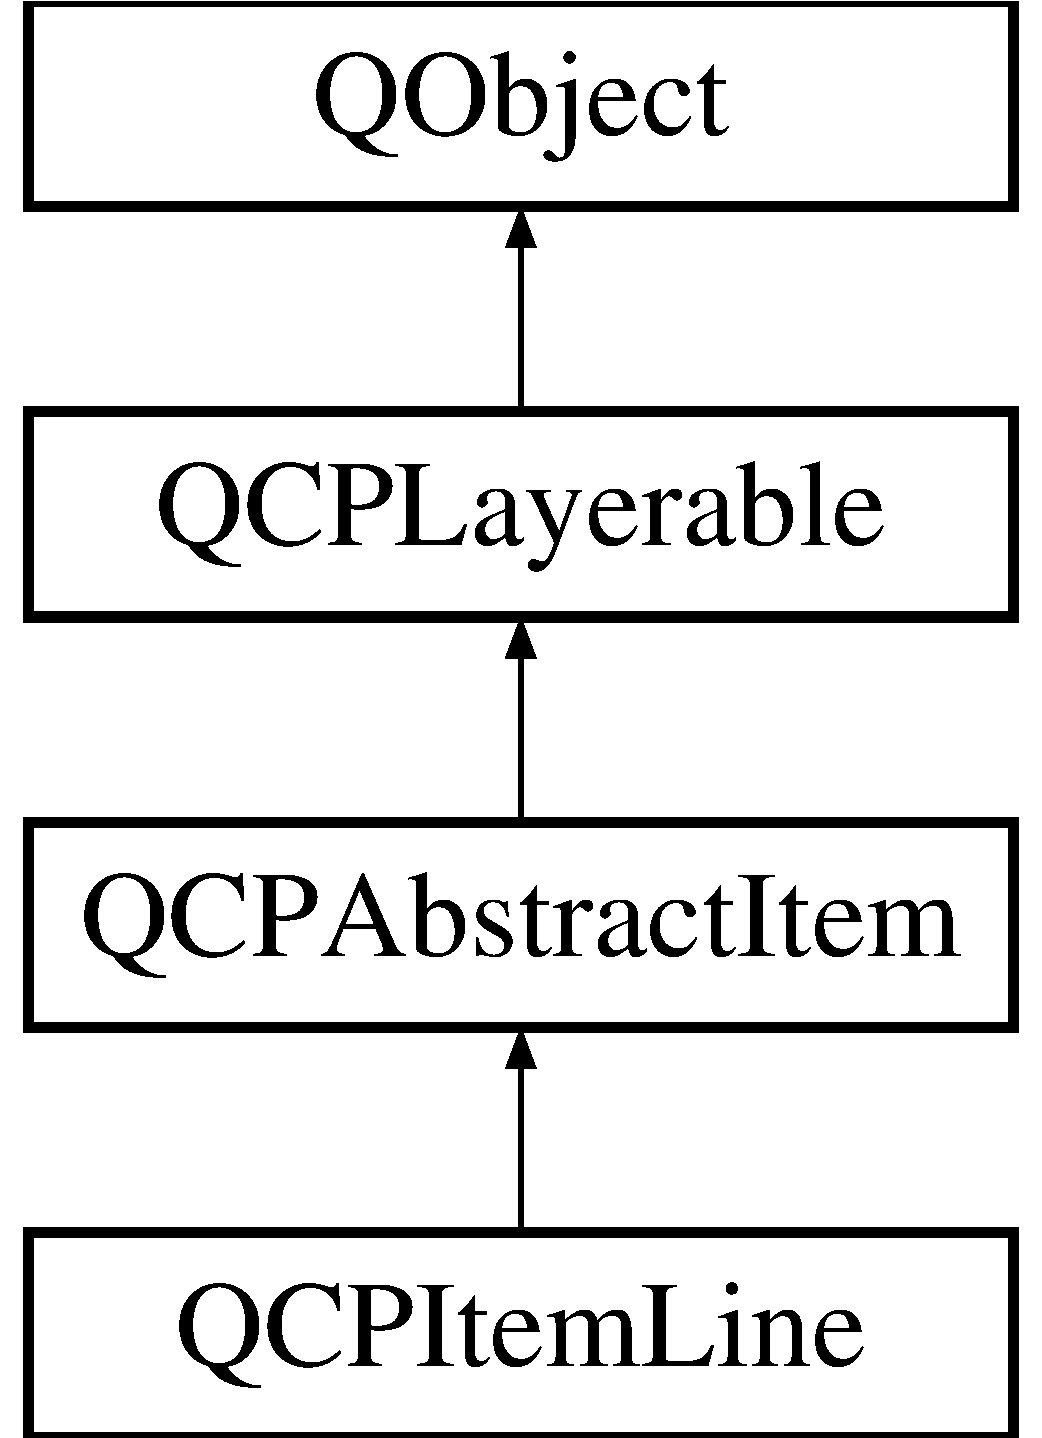
\includegraphics[height=4.000000cm]{class_q_c_p_item_line}
\end{center}
\end{figure}
\subsection*{Public Member Functions}
\begin{DoxyCompactItemize}
\item 
\hyperlink{class_q_c_p_item_line_a17804b7f64961c6accf25b61e85142e3}{Q\+C\+P\+Item\+Line} (\hyperlink{class_q_custom_plot}{Q\+Custom\+Plot} $\ast$parent\+Plot)
\item 
\hypertarget{class_q_c_p_item_line_a712e5a7f59db3f4c588dfc370a63e225}{}\label{class_q_c_p_item_line_a712e5a7f59db3f4c588dfc370a63e225} 
Q\+Pen {\bfseries pen} () const
\item 
\hypertarget{class_q_c_p_item_line_ae1782c4fbecd38054ec3d49d8572a5e5}{}\label{class_q_c_p_item_line_ae1782c4fbecd38054ec3d49d8572a5e5} 
Q\+Pen {\bfseries selected\+Pen} () const
\item 
\hypertarget{class_q_c_p_item_line_a6cdc9e87e17418d4b0e66eaa0f041407}{}\label{class_q_c_p_item_line_a6cdc9e87e17418d4b0e66eaa0f041407} 
\hyperlink{class_q_c_p_line_ending}{Q\+C\+P\+Line\+Ending} {\bfseries head} () const
\item 
\hypertarget{class_q_c_p_item_line_ac085d3939ec11d7a4d592dc2ed578360}{}\label{class_q_c_p_item_line_ac085d3939ec11d7a4d592dc2ed578360} 
\hyperlink{class_q_c_p_line_ending}{Q\+C\+P\+Line\+Ending} {\bfseries tail} () const
\item 
void \hyperlink{class_q_c_p_item_line_a572528dab61c1abe205822fbd5db4b27}{set\+Pen} (const Q\+Pen \&pen)
\item 
void \hyperlink{class_q_c_p_item_line_a3e2fec44503277e77717e9c24f87f1ea}{set\+Selected\+Pen} (const Q\+Pen \&pen)
\item 
void \hyperlink{class_q_c_p_item_line_aebf3d687114d584e0459db6759e2c3c3}{set\+Head} (const \hyperlink{class_q_c_p_line_ending}{Q\+C\+P\+Line\+Ending} \&head)
\item 
void \hyperlink{class_q_c_p_item_line_ac264222c3297a7efe33df9345c811a5f}{set\+Tail} (const \hyperlink{class_q_c_p_line_ending}{Q\+C\+P\+Line\+Ending} \&tail)
\item 
virtual double \hyperlink{class_q_c_p_item_line_ae6cc5183f568e5fa9d7827abe4d405b5}{select\+Test} (const Q\+PointF \&pos, bool only\+Selectable, Q\+Variant $\ast$details=0) const
\end{DoxyCompactItemize}
\subsection*{Public Attributes}
\begin{DoxyCompactItemize}
\item 
\hypertarget{class_q_c_p_item_line_a602da607a09498b0f152ada1d6851bc5}{}\label{class_q_c_p_item_line_a602da607a09498b0f152ada1d6851bc5} 
\hyperlink{class_q_c_p_item_position}{Q\+C\+P\+Item\+Position} $\ast$const {\bfseries start}
\item 
\hypertarget{class_q_c_p_item_line_a15598864c1c22a2497a1979c4980c4e1}{}\label{class_q_c_p_item_line_a15598864c1c22a2497a1979c4980c4e1} 
\hyperlink{class_q_c_p_item_position}{Q\+C\+P\+Item\+Position} $\ast$const {\bfseries end}
\end{DoxyCompactItemize}
\subsection*{Protected Member Functions}
\begin{DoxyCompactItemize}
\item 
\hypertarget{class_q_c_p_item_line_a1fc045dd33919f8006df0692aeb0e84a}{}\label{class_q_c_p_item_line_a1fc045dd33919f8006df0692aeb0e84a} 
virtual void {\bfseries draw} (\hyperlink{class_q_c_p_painter}{Q\+C\+P\+Painter} $\ast$painter)
\item 
\hypertarget{class_q_c_p_item_line_ae61e504ad3b94aa86bfd02f734fb17b0}{}\label{class_q_c_p_item_line_ae61e504ad3b94aa86bfd02f734fb17b0} 
Q\+LineF {\bfseries get\+Rect\+Clipped\+Line} (const Q\+Vector2D \&start, const Q\+Vector2D \&end, const Q\+Rect \&rect) const
\item 
\hypertarget{class_q_c_p_item_line_af8b5370462515b279578d8b4a57bd3b4}{}\label{class_q_c_p_item_line_af8b5370462515b279578d8b4a57bd3b4} 
Q\+Pen {\bfseries main\+Pen} () const
\end{DoxyCompactItemize}
\subsection*{Protected Attributes}
\begin{DoxyCompactItemize}
\item 
\hypertarget{class_q_c_p_item_line_abbb544d5bb927dfe4e81a7f3ca4c65ac}{}\label{class_q_c_p_item_line_abbb544d5bb927dfe4e81a7f3ca4c65ac} 
Q\+Pen {\bfseries m\+Pen}
\item 
\hypertarget{class_q_c_p_item_line_aff858ad6dde3b90024814ca4b116f278}{}\label{class_q_c_p_item_line_aff858ad6dde3b90024814ca4b116f278} 
Q\+Pen {\bfseries m\+Selected\+Pen}
\item 
\hypertarget{class_q_c_p_item_line_a51603f28ab7ddb1c1a95ea384791d3ed}{}\label{class_q_c_p_item_line_a51603f28ab7ddb1c1a95ea384791d3ed} 
\hyperlink{class_q_c_p_line_ending}{Q\+C\+P\+Line\+Ending} {\bfseries m\+Head}
\item 
\hypertarget{class_q_c_p_item_line_ab8ed61dfe15bbb1cbf9b95eae95e242f}{}\label{class_q_c_p_item_line_ab8ed61dfe15bbb1cbf9b95eae95e242f} 
\hyperlink{class_q_c_p_line_ending}{Q\+C\+P\+Line\+Ending} {\bfseries m\+Tail}
\end{DoxyCompactItemize}
\subsection*{Additional Inherited Members}


\subsection{Detailed Description}
A line from one point to another. 

 It has two positions, {\itshape start} and {\itshape end}, which define the end points of the line.

With \hyperlink{class_q_c_p_item_line_aebf3d687114d584e0459db6759e2c3c3}{set\+Head} and \hyperlink{class_q_c_p_item_line_ac264222c3297a7efe33df9345c811a5f}{set\+Tail} you may set different line ending styles, e.\+g. to create an arrow. 

\subsection{Constructor \& Destructor Documentation}
\hypertarget{class_q_c_p_item_line_a17804b7f64961c6accf25b61e85142e3}{}\label{class_q_c_p_item_line_a17804b7f64961c6accf25b61e85142e3} 
\index{Q\+C\+P\+Item\+Line@{Q\+C\+P\+Item\+Line}!Q\+C\+P\+Item\+Line@{Q\+C\+P\+Item\+Line}}
\index{Q\+C\+P\+Item\+Line@{Q\+C\+P\+Item\+Line}!Q\+C\+P\+Item\+Line@{Q\+C\+P\+Item\+Line}}
\subsubsection{\texorpdfstring{Q\+C\+P\+Item\+Line()}{QCPItemLine()}}
{\footnotesize\ttfamily Q\+C\+P\+Item\+Line\+::\+Q\+C\+P\+Item\+Line (\begin{DoxyParamCaption}\item[{\hyperlink{class_q_custom_plot}{Q\+Custom\+Plot} $\ast$}]{parent\+Plot }\end{DoxyParamCaption})}

Creates a line item and sets default values.

The constructed item can be added to the plot with \hyperlink{class_q_custom_plot_aa500620379262321685cb7a7674cbd2a}{Q\+Custom\+Plot\+::add\+Item}. 

\subsection{Member Function Documentation}
\hypertarget{class_q_c_p_item_line_ae6cc5183f568e5fa9d7827abe4d405b5}{}\label{class_q_c_p_item_line_ae6cc5183f568e5fa9d7827abe4d405b5} 
\index{Q\+C\+P\+Item\+Line@{Q\+C\+P\+Item\+Line}!select\+Test@{select\+Test}}
\index{select\+Test@{select\+Test}!Q\+C\+P\+Item\+Line@{Q\+C\+P\+Item\+Line}}
\subsubsection{\texorpdfstring{select\+Test()}{selectTest()}}
{\footnotesize\ttfamily double Q\+C\+P\+Item\+Line\+::select\+Test (\begin{DoxyParamCaption}\item[{const Q\+PointF \&}]{pos,  }\item[{bool}]{only\+Selectable,  }\item[{Q\+Variant $\ast$}]{details = {\ttfamily 0} }\end{DoxyParamCaption}) const\hspace{0.3cm}{\ttfamily [virtual]}}

This function is used to decide whether a click hits a layerable object or not.

{\itshape pos} is a point in pixel coordinates on the \hyperlink{class_q_custom_plot}{Q\+Custom\+Plot} surface. This function returns the shortest pixel distance of this point to the object. If the object is either invisible or the distance couldn\textquotesingle{}t be determined, -\/1.\+0 is returned. Further, if {\itshape only\+Selectable} is true and the object is not selectable, -\/1.\+0 is returned, too.

If the object is represented not by single lines but by an area like a \hyperlink{class_q_c_p_item_text}{Q\+C\+P\+Item\+Text} or the bars of a \hyperlink{class_q_c_p_bars}{Q\+C\+P\+Bars} plottable, a click inside the area should also be considered a hit. In these cases this function thus returns a constant value greater zero but still below the parent plot\textquotesingle{}s selection tolerance. (typically the selection\+Tolerance multiplied by 0.\+99).

Providing a constant value for area objects allows selecting line objects even when they are obscured by such area objects, by clicking close to the lines (i.\+e. closer than 0.\+99$\ast$selection\+Tolerance).

The actual setting of the selection state is not done by this function. This is handled by the parent \hyperlink{class_q_custom_plot}{Q\+Custom\+Plot} when the mouse\+Release\+Event occurs, and the finally selected object is notified via the select\+Event/deselect\+Event methods.

{\itshape details} is an optional output parameter. Every layerable subclass may place any information in {\itshape details}. This information will be passed to select\+Event when the parent \hyperlink{class_q_custom_plot}{Q\+Custom\+Plot} decides on the basis of this select\+Test call, that the object was successfully selected. The subsequent call to select\+Event will carry the {\itshape details}. This is useful for multi-\/part objects (like \hyperlink{class_q_c_p_axis}{Q\+C\+P\+Axis}). This way, a possibly complex calculation to decide which part was clicked is only done once in \hyperlink{class_q_c_p_item_line_ae6cc5183f568e5fa9d7827abe4d405b5}{select\+Test}. The result (i.\+e. the actually clicked part) can then be placed in {\itshape details}. So in the subsequent select\+Event, the decision which part was selected doesn\textquotesingle{}t have to be done a second time for a single selection operation.

You may pass 0 as {\itshape details} to indicate that you are not interested in those selection details.

\begin{DoxySeeAlso}{See also}
select\+Event, deselect\+Event, \hyperlink{class_q_custom_plot_a5ee1e2f6ae27419deca53e75907c27e5}{Q\+Custom\+Plot\+::set\+Interactions} 
\end{DoxySeeAlso}


Implements \hyperlink{class_q_c_p_abstract_item_a96d522d10ffc0413b9a366c6f7f0476b}{Q\+C\+P\+Abstract\+Item}.

\hypertarget{class_q_c_p_item_line_aebf3d687114d584e0459db6759e2c3c3}{}\label{class_q_c_p_item_line_aebf3d687114d584e0459db6759e2c3c3} 
\index{Q\+C\+P\+Item\+Line@{Q\+C\+P\+Item\+Line}!set\+Head@{set\+Head}}
\index{set\+Head@{set\+Head}!Q\+C\+P\+Item\+Line@{Q\+C\+P\+Item\+Line}}
\subsubsection{\texorpdfstring{set\+Head()}{setHead()}}
{\footnotesize\ttfamily void Q\+C\+P\+Item\+Line\+::set\+Head (\begin{DoxyParamCaption}\item[{const \hyperlink{class_q_c_p_line_ending}{Q\+C\+P\+Line\+Ending} \&}]{head }\end{DoxyParamCaption})}

Sets the line ending style of the head. The head corresponds to the {\itshape end} position.

Note that due to the overloaded \hyperlink{class_q_c_p_line_ending}{Q\+C\+P\+Line\+Ending} constructor, you may directly specify a \hyperlink{class_q_c_p_line_ending_a5ef16e6876b4b74959c7261d8d4c2cd5}{Q\+C\+P\+Line\+Ending\+::\+Ending\+Style} here, e.\+g.
\begin{DoxyCode}
\hyperlink{class_q_c_p_item_line_aebf3d687114d584e0459db6759e2c3c3}{setHead}(\hyperlink{class_q_c_p_line_ending_a5ef16e6876b4b74959c7261d8d4c2cd5ab9964d0d03f812d1e79de15edbeb2cbf}{QCPLineEnding::esSpikeArrow}) 
\end{DoxyCode}


\begin{DoxySeeAlso}{See also}
\hyperlink{class_q_c_p_item_line_ac264222c3297a7efe33df9345c811a5f}{set\+Tail} 
\end{DoxySeeAlso}
\hypertarget{class_q_c_p_item_line_a572528dab61c1abe205822fbd5db4b27}{}\label{class_q_c_p_item_line_a572528dab61c1abe205822fbd5db4b27} 
\index{Q\+C\+P\+Item\+Line@{Q\+C\+P\+Item\+Line}!set\+Pen@{set\+Pen}}
\index{set\+Pen@{set\+Pen}!Q\+C\+P\+Item\+Line@{Q\+C\+P\+Item\+Line}}
\subsubsection{\texorpdfstring{set\+Pen()}{setPen()}}
{\footnotesize\ttfamily void Q\+C\+P\+Item\+Line\+::set\+Pen (\begin{DoxyParamCaption}\item[{const Q\+Pen \&}]{pen }\end{DoxyParamCaption})}

Sets the pen that will be used to draw the line

\begin{DoxySeeAlso}{See also}
\hyperlink{class_q_c_p_item_line_a3e2fec44503277e77717e9c24f87f1ea}{set\+Selected\+Pen} 
\end{DoxySeeAlso}
\hypertarget{class_q_c_p_item_line_a3e2fec44503277e77717e9c24f87f1ea}{}\label{class_q_c_p_item_line_a3e2fec44503277e77717e9c24f87f1ea} 
\index{Q\+C\+P\+Item\+Line@{Q\+C\+P\+Item\+Line}!set\+Selected\+Pen@{set\+Selected\+Pen}}
\index{set\+Selected\+Pen@{set\+Selected\+Pen}!Q\+C\+P\+Item\+Line@{Q\+C\+P\+Item\+Line}}
\subsubsection{\texorpdfstring{set\+Selected\+Pen()}{setSelectedPen()}}
{\footnotesize\ttfamily void Q\+C\+P\+Item\+Line\+::set\+Selected\+Pen (\begin{DoxyParamCaption}\item[{const Q\+Pen \&}]{pen }\end{DoxyParamCaption})}

Sets the pen that will be used to draw the line when selected

\begin{DoxySeeAlso}{See also}
\hyperlink{class_q_c_p_item_line_a572528dab61c1abe205822fbd5db4b27}{set\+Pen}, \hyperlink{class_q_c_p_abstract_item_a203de94ad586cc44d16c9565f49d3378}{set\+Selected} 
\end{DoxySeeAlso}
\hypertarget{class_q_c_p_item_line_ac264222c3297a7efe33df9345c811a5f}{}\label{class_q_c_p_item_line_ac264222c3297a7efe33df9345c811a5f} 
\index{Q\+C\+P\+Item\+Line@{Q\+C\+P\+Item\+Line}!set\+Tail@{set\+Tail}}
\index{set\+Tail@{set\+Tail}!Q\+C\+P\+Item\+Line@{Q\+C\+P\+Item\+Line}}
\subsubsection{\texorpdfstring{set\+Tail()}{setTail()}}
{\footnotesize\ttfamily void Q\+C\+P\+Item\+Line\+::set\+Tail (\begin{DoxyParamCaption}\item[{const \hyperlink{class_q_c_p_line_ending}{Q\+C\+P\+Line\+Ending} \&}]{tail }\end{DoxyParamCaption})}

Sets the line ending style of the tail. The tail corresponds to the {\itshape start} position.

Note that due to the overloaded \hyperlink{class_q_c_p_line_ending}{Q\+C\+P\+Line\+Ending} constructor, you may directly specify a \hyperlink{class_q_c_p_line_ending_a5ef16e6876b4b74959c7261d8d4c2cd5}{Q\+C\+P\+Line\+Ending\+::\+Ending\+Style} here, e.\+g.
\begin{DoxyCode}
\hyperlink{class_q_c_p_item_line_ac264222c3297a7efe33df9345c811a5f}{setTail}(\hyperlink{class_q_c_p_line_ending_a5ef16e6876b4b74959c7261d8d4c2cd5ab9964d0d03f812d1e79de15edbeb2cbf}{QCPLineEnding::esSpikeArrow}) 
\end{DoxyCode}


\begin{DoxySeeAlso}{See also}
\hyperlink{class_q_c_p_item_line_aebf3d687114d584e0459db6759e2c3c3}{set\+Head} 
\end{DoxySeeAlso}


The documentation for this class was generated from the following files\+:\begin{DoxyCompactItemize}
\item 
F\+E\+S\+S-\/\+G\+U\+I/\hyperlink{qcustomplot_8h}{qcustomplot.\+h}\item 
F\+E\+S\+S-\/\+G\+U\+I/\hyperlink{qcustomplot_8cpp}{qcustomplot.\+cpp}\end{DoxyCompactItemize}

\hypertarget{class_q_c_p_item_pixmap}{}\section{Q\+C\+P\+Item\+Pixmap Class Reference}
\label{class_q_c_p_item_pixmap}\index{Q\+C\+P\+Item\+Pixmap@{Q\+C\+P\+Item\+Pixmap}}


An arbitrary pixmap.  


Inheritance diagram for Q\+C\+P\+Item\+Pixmap\+:\begin{figure}[H]
\begin{center}
\leavevmode
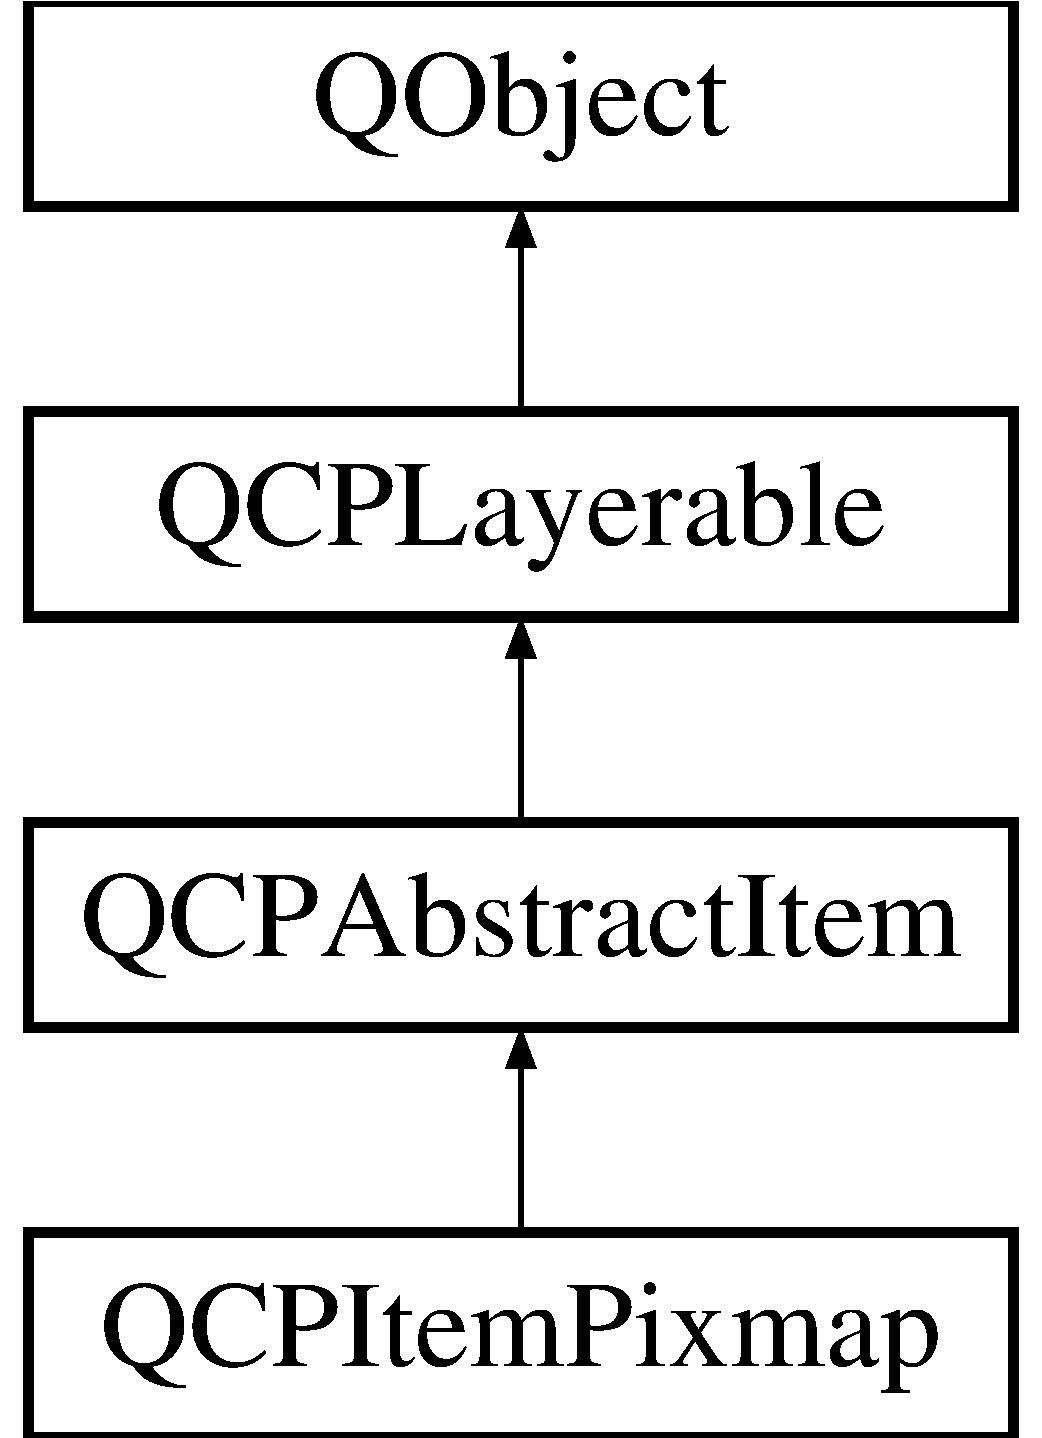
\includegraphics[height=4.000000cm]{class_q_c_p_item_pixmap}
\end{center}
\end{figure}
\subsection*{Public Member Functions}
\begin{DoxyCompactItemize}
\item 
\hyperlink{class_q_c_p_item_pixmap_aa6de42a37261b21a5480e7da122345c3}{Q\+C\+P\+Item\+Pixmap} (\hyperlink{class_q_custom_plot}{Q\+Custom\+Plot} $\ast$parent\+Plot)
\item 
\hypertarget{class_q_c_p_item_pixmap_a7daef7e0c432902d69e7db3e0e217a1f}{}\label{class_q_c_p_item_pixmap_a7daef7e0c432902d69e7db3e0e217a1f} 
Q\+Pixmap {\bfseries pixmap} () const
\item 
\hypertarget{class_q_c_p_item_pixmap_a8768534b5f3080abfc007db198373327}{}\label{class_q_c_p_item_pixmap_a8768534b5f3080abfc007db198373327} 
bool {\bfseries scaled} () const
\item 
\hypertarget{class_q_c_p_item_pixmap_a662cbca12e6cdcd2a94b0b08879292fd}{}\label{class_q_c_p_item_pixmap_a662cbca12e6cdcd2a94b0b08879292fd} 
Qt\+::\+Aspect\+Ratio\+Mode {\bfseries aspect\+Ratio\+Mode} () const
\item 
\hypertarget{class_q_c_p_item_pixmap_ab963aa9693d49c323948f2820a5785b6}{}\label{class_q_c_p_item_pixmap_ab963aa9693d49c323948f2820a5785b6} 
Qt\+::\+Transformation\+Mode {\bfseries transformation\+Mode} () const
\item 
\hypertarget{class_q_c_p_item_pixmap_a6ae9922eba6386a5ac4e2a569ec29e1f}{}\label{class_q_c_p_item_pixmap_a6ae9922eba6386a5ac4e2a569ec29e1f} 
Q\+Pen {\bfseries pen} () const
\item 
\hypertarget{class_q_c_p_item_pixmap_a23806a20efcb172f0309e18809dc49d8}{}\label{class_q_c_p_item_pixmap_a23806a20efcb172f0309e18809dc49d8} 
Q\+Pen {\bfseries selected\+Pen} () const
\item 
void \hyperlink{class_q_c_p_item_pixmap_a726b69ea4025edf48f9b29b6450548a7}{set\+Pixmap} (const Q\+Pixmap \&pixmap)
\item 
void \hyperlink{class_q_c_p_item_pixmap_ab4d44529a1c6c8d37d0ea7560e042777}{set\+Scaled} (bool scaled, Qt\+::\+Aspect\+Ratio\+Mode aspect\+Ratio\+Mode=Qt\+::\+Keep\+Aspect\+Ratio, Qt\+::\+Transformation\+Mode transformation\+Mode=Qt\+::\+Smooth\+Transformation)
\item 
void \hyperlink{class_q_c_p_item_pixmap_acdade1305edb4b5cae14f97fd132065f}{set\+Pen} (const Q\+Pen \&pen)
\item 
void \hyperlink{class_q_c_p_item_pixmap_afc5e479e88e53740176ce77cb70dd67a}{set\+Selected\+Pen} (const Q\+Pen \&pen)
\item 
virtual double \hyperlink{class_q_c_p_item_pixmap_a7583a98ebd3f35d2ac5d6c05fad25a6c}{select\+Test} (const Q\+PointF \&pos, bool only\+Selectable, Q\+Variant $\ast$details=0) const
\end{DoxyCompactItemize}
\subsection*{Public Attributes}
\begin{DoxyCompactItemize}
\item 
\hypertarget{class_q_c_p_item_pixmap_a43c281ef6ad46f3cf04f365289abe51a}{}\label{class_q_c_p_item_pixmap_a43c281ef6ad46f3cf04f365289abe51a} 
\hyperlink{class_q_c_p_item_position}{Q\+C\+P\+Item\+Position} $\ast$const {\bfseries top\+Left}
\item 
\hypertarget{class_q_c_p_item_pixmap_abcc38063f9502b876bf6615c45cc0994}{}\label{class_q_c_p_item_pixmap_abcc38063f9502b876bf6615c45cc0994} 
\hyperlink{class_q_c_p_item_position}{Q\+C\+P\+Item\+Position} $\ast$const {\bfseries bottom\+Right}
\item 
\hypertarget{class_q_c_p_item_pixmap_af7a156590b1d59ab21b453c430c56a7c}{}\label{class_q_c_p_item_pixmap_af7a156590b1d59ab21b453c430c56a7c} 
\hyperlink{class_q_c_p_item_anchor}{Q\+C\+P\+Item\+Anchor} $\ast$const {\bfseries top}
\item 
\hypertarget{class_q_c_p_item_pixmap_a72eabd0010be41a4ec1b22aa983d2aa1}{}\label{class_q_c_p_item_pixmap_a72eabd0010be41a4ec1b22aa983d2aa1} 
\hyperlink{class_q_c_p_item_anchor}{Q\+C\+P\+Item\+Anchor} $\ast$const {\bfseries top\+Right}
\item 
\hypertarget{class_q_c_p_item_pixmap_ac9c0fd231f9e285765978a05d13f8280}{}\label{class_q_c_p_item_pixmap_ac9c0fd231f9e285765978a05d13f8280} 
\hyperlink{class_q_c_p_item_anchor}{Q\+C\+P\+Item\+Anchor} $\ast$const {\bfseries right}
\item 
\hypertarget{class_q_c_p_item_pixmap_ad7da77f530868e846151eff8a28fb948}{}\label{class_q_c_p_item_pixmap_ad7da77f530868e846151eff8a28fb948} 
\hyperlink{class_q_c_p_item_anchor}{Q\+C\+P\+Item\+Anchor} $\ast$const {\bfseries bottom}
\item 
\hypertarget{class_q_c_p_item_pixmap_a01943e569233382b3627e24636b0fff2}{}\label{class_q_c_p_item_pixmap_a01943e569233382b3627e24636b0fff2} 
\hyperlink{class_q_c_p_item_anchor}{Q\+C\+P\+Item\+Anchor} $\ast$const {\bfseries bottom\+Left}
\item 
\hypertarget{class_q_c_p_item_pixmap_a8c85fcb8cb8ce292859a0499d16539b1}{}\label{class_q_c_p_item_pixmap_a8c85fcb8cb8ce292859a0499d16539b1} 
\hyperlink{class_q_c_p_item_anchor}{Q\+C\+P\+Item\+Anchor} $\ast$const {\bfseries left}
\end{DoxyCompactItemize}
\subsection*{Protected Types}
\begin{DoxyCompactItemize}
\item 
\hypertarget{class_q_c_p_item_pixmap_a0ea7f65edb7395e02de521915f221174}{}\label{class_q_c_p_item_pixmap_a0ea7f65edb7395e02de521915f221174} 
enum {\bfseries Anchor\+Index} \{ \newline
{\bfseries ai\+Top}, 
{\bfseries ai\+Top\+Right}, 
{\bfseries ai\+Right}, 
{\bfseries ai\+Bottom}, 
\newline
{\bfseries ai\+Bottom\+Left}, 
{\bfseries ai\+Left}
 \}
\end{DoxyCompactItemize}
\subsection*{Protected Member Functions}
\begin{DoxyCompactItemize}
\item 
\hypertarget{class_q_c_p_item_pixmap_a879e8076c2db01a38b34cfa73ec95d2f}{}\label{class_q_c_p_item_pixmap_a879e8076c2db01a38b34cfa73ec95d2f} 
virtual void {\bfseries draw} (\hyperlink{class_q_c_p_painter}{Q\+C\+P\+Painter} $\ast$painter)
\item 
\hypertarget{class_q_c_p_item_pixmap_a24d4072c0e50c608ddcc0840d853fc03}{}\label{class_q_c_p_item_pixmap_a24d4072c0e50c608ddcc0840d853fc03} 
virtual Q\+PointF {\bfseries anchor\+Pixel\+Point} (int anchor\+Id) const
\item 
\hypertarget{class_q_c_p_item_pixmap_a8bced3027b326b290726cd1979c7cfc6}{}\label{class_q_c_p_item_pixmap_a8bced3027b326b290726cd1979c7cfc6} 
void {\bfseries update\+Scaled\+Pixmap} (Q\+Rect final\+Rect=Q\+Rect(), bool flip\+Horz=false, bool flip\+Vert=false)
\item 
\hypertarget{class_q_c_p_item_pixmap_a4e7d803e5093c457a109f8fae56677c2}{}\label{class_q_c_p_item_pixmap_a4e7d803e5093c457a109f8fae56677c2} 
Q\+Rect {\bfseries get\+Final\+Rect} (bool $\ast$flipped\+Horz=0, bool $\ast$flipped\+Vert=0) const
\item 
\hypertarget{class_q_c_p_item_pixmap_aad6dddd67163831538d40023a98a9fe7}{}\label{class_q_c_p_item_pixmap_aad6dddd67163831538d40023a98a9fe7} 
Q\+Pen {\bfseries main\+Pen} () const
\end{DoxyCompactItemize}
\subsection*{Protected Attributes}
\begin{DoxyCompactItemize}
\item 
\hypertarget{class_q_c_p_item_pixmap_a1396cce7f26c7b8e9512906284380c4d}{}\label{class_q_c_p_item_pixmap_a1396cce7f26c7b8e9512906284380c4d} 
Q\+Pixmap {\bfseries m\+Pixmap}
\item 
\hypertarget{class_q_c_p_item_pixmap_a2ebc66e15b9f1264563d58f29ba1bc00}{}\label{class_q_c_p_item_pixmap_a2ebc66e15b9f1264563d58f29ba1bc00} 
Q\+Pixmap {\bfseries m\+Scaled\+Pixmap}
\item 
\hypertarget{class_q_c_p_item_pixmap_a8fe670a529cd46a9b8afd9fc1203bc3f}{}\label{class_q_c_p_item_pixmap_a8fe670a529cd46a9b8afd9fc1203bc3f} 
bool {\bfseries m\+Scaled}
\item 
\hypertarget{class_q_c_p_item_pixmap_a223134abd4cf3d6c368573c622bd2e1c}{}\label{class_q_c_p_item_pixmap_a223134abd4cf3d6c368573c622bd2e1c} 
bool {\bfseries m\+Scaled\+Pixmap\+Invalidated}
\item 
\hypertarget{class_q_c_p_item_pixmap_a8dc6b6c1e106ac523efae22d5fe55bab}{}\label{class_q_c_p_item_pixmap_a8dc6b6c1e106ac523efae22d5fe55bab} 
Qt\+::\+Aspect\+Ratio\+Mode {\bfseries m\+Aspect\+Ratio\+Mode}
\item 
\hypertarget{class_q_c_p_item_pixmap_ac9ecad3b9842363754e32eda2cf821bd}{}\label{class_q_c_p_item_pixmap_ac9ecad3b9842363754e32eda2cf821bd} 
Qt\+::\+Transformation\+Mode {\bfseries m\+Transformation\+Mode}
\item 
\hypertarget{class_q_c_p_item_pixmap_acfee1124eb51a1887aaf8de10777c7a1}{}\label{class_q_c_p_item_pixmap_acfee1124eb51a1887aaf8de10777c7a1} 
Q\+Pen {\bfseries m\+Pen}
\item 
\hypertarget{class_q_c_p_item_pixmap_a0949e5bb6a261fc4e9668e28e2effcfa}{}\label{class_q_c_p_item_pixmap_a0949e5bb6a261fc4e9668e28e2effcfa} 
Q\+Pen {\bfseries m\+Selected\+Pen}
\end{DoxyCompactItemize}
\subsection*{Additional Inherited Members}


\subsection{Detailed Description}
An arbitrary pixmap. 

 It has two positions, {\itshape top\+Left} and {\itshape bottom\+Right}, which define the rectangle the pixmap will be drawn in. Depending on the scale setting (\hyperlink{class_q_c_p_item_pixmap_ab4d44529a1c6c8d37d0ea7560e042777}{set\+Scaled}), the pixmap will be either scaled to fit the rectangle or be drawn aligned to the top\+Left position.

If scaling is enabled and {\itshape top\+Left} is further to the bottom/right than {\itshape bottom\+Right} (as shown on the right side of the example image), the pixmap will be flipped in the respective orientations. 

\subsection{Constructor \& Destructor Documentation}
\hypertarget{class_q_c_p_item_pixmap_aa6de42a37261b21a5480e7da122345c3}{}\label{class_q_c_p_item_pixmap_aa6de42a37261b21a5480e7da122345c3} 
\index{Q\+C\+P\+Item\+Pixmap@{Q\+C\+P\+Item\+Pixmap}!Q\+C\+P\+Item\+Pixmap@{Q\+C\+P\+Item\+Pixmap}}
\index{Q\+C\+P\+Item\+Pixmap@{Q\+C\+P\+Item\+Pixmap}!Q\+C\+P\+Item\+Pixmap@{Q\+C\+P\+Item\+Pixmap}}
\subsubsection{\texorpdfstring{Q\+C\+P\+Item\+Pixmap()}{QCPItemPixmap()}}
{\footnotesize\ttfamily Q\+C\+P\+Item\+Pixmap\+::\+Q\+C\+P\+Item\+Pixmap (\begin{DoxyParamCaption}\item[{\hyperlink{class_q_custom_plot}{Q\+Custom\+Plot} $\ast$}]{parent\+Plot }\end{DoxyParamCaption})}

Creates a rectangle item and sets default values.

The constructed item can be added to the plot with \hyperlink{class_q_custom_plot_aa500620379262321685cb7a7674cbd2a}{Q\+Custom\+Plot\+::add\+Item}. 

\subsection{Member Function Documentation}
\hypertarget{class_q_c_p_item_pixmap_a7583a98ebd3f35d2ac5d6c05fad25a6c}{}\label{class_q_c_p_item_pixmap_a7583a98ebd3f35d2ac5d6c05fad25a6c} 
\index{Q\+C\+P\+Item\+Pixmap@{Q\+C\+P\+Item\+Pixmap}!select\+Test@{select\+Test}}
\index{select\+Test@{select\+Test}!Q\+C\+P\+Item\+Pixmap@{Q\+C\+P\+Item\+Pixmap}}
\subsubsection{\texorpdfstring{select\+Test()}{selectTest()}}
{\footnotesize\ttfamily double Q\+C\+P\+Item\+Pixmap\+::select\+Test (\begin{DoxyParamCaption}\item[{const Q\+PointF \&}]{pos,  }\item[{bool}]{only\+Selectable,  }\item[{Q\+Variant $\ast$}]{details = {\ttfamily 0} }\end{DoxyParamCaption}) const\hspace{0.3cm}{\ttfamily [virtual]}}

This function is used to decide whether a click hits a layerable object or not.

{\itshape pos} is a point in pixel coordinates on the \hyperlink{class_q_custom_plot}{Q\+Custom\+Plot} surface. This function returns the shortest pixel distance of this point to the object. If the object is either invisible or the distance couldn\textquotesingle{}t be determined, -\/1.\+0 is returned. Further, if {\itshape only\+Selectable} is true and the object is not selectable, -\/1.\+0 is returned, too.

If the object is represented not by single lines but by an area like a \hyperlink{class_q_c_p_item_text}{Q\+C\+P\+Item\+Text} or the bars of a \hyperlink{class_q_c_p_bars}{Q\+C\+P\+Bars} plottable, a click inside the area should also be considered a hit. In these cases this function thus returns a constant value greater zero but still below the parent plot\textquotesingle{}s selection tolerance. (typically the selection\+Tolerance multiplied by 0.\+99).

Providing a constant value for area objects allows selecting line objects even when they are obscured by such area objects, by clicking close to the lines (i.\+e. closer than 0.\+99$\ast$selection\+Tolerance).

The actual setting of the selection state is not done by this function. This is handled by the parent \hyperlink{class_q_custom_plot}{Q\+Custom\+Plot} when the mouse\+Release\+Event occurs, and the finally selected object is notified via the select\+Event/deselect\+Event methods.

{\itshape details} is an optional output parameter. Every layerable subclass may place any information in {\itshape details}. This information will be passed to select\+Event when the parent \hyperlink{class_q_custom_plot}{Q\+Custom\+Plot} decides on the basis of this select\+Test call, that the object was successfully selected. The subsequent call to select\+Event will carry the {\itshape details}. This is useful for multi-\/part objects (like \hyperlink{class_q_c_p_axis}{Q\+C\+P\+Axis}). This way, a possibly complex calculation to decide which part was clicked is only done once in \hyperlink{class_q_c_p_item_pixmap_a7583a98ebd3f35d2ac5d6c05fad25a6c}{select\+Test}. The result (i.\+e. the actually clicked part) can then be placed in {\itshape details}. So in the subsequent select\+Event, the decision which part was selected doesn\textquotesingle{}t have to be done a second time for a single selection operation.

You may pass 0 as {\itshape details} to indicate that you are not interested in those selection details.

\begin{DoxySeeAlso}{See also}
select\+Event, deselect\+Event, \hyperlink{class_q_custom_plot_a5ee1e2f6ae27419deca53e75907c27e5}{Q\+Custom\+Plot\+::set\+Interactions} 
\end{DoxySeeAlso}


Implements \hyperlink{class_q_c_p_abstract_item_a96d522d10ffc0413b9a366c6f7f0476b}{Q\+C\+P\+Abstract\+Item}.

\hypertarget{class_q_c_p_item_pixmap_acdade1305edb4b5cae14f97fd132065f}{}\label{class_q_c_p_item_pixmap_acdade1305edb4b5cae14f97fd132065f} 
\index{Q\+C\+P\+Item\+Pixmap@{Q\+C\+P\+Item\+Pixmap}!set\+Pen@{set\+Pen}}
\index{set\+Pen@{set\+Pen}!Q\+C\+P\+Item\+Pixmap@{Q\+C\+P\+Item\+Pixmap}}
\subsubsection{\texorpdfstring{set\+Pen()}{setPen()}}
{\footnotesize\ttfamily void Q\+C\+P\+Item\+Pixmap\+::set\+Pen (\begin{DoxyParamCaption}\item[{const Q\+Pen \&}]{pen }\end{DoxyParamCaption})}

Sets the pen that will be used to draw a border around the pixmap.

\begin{DoxySeeAlso}{See also}
\hyperlink{class_q_c_p_item_pixmap_afc5e479e88e53740176ce77cb70dd67a}{set\+Selected\+Pen}, set\+Brush 
\end{DoxySeeAlso}
\hypertarget{class_q_c_p_item_pixmap_a726b69ea4025edf48f9b29b6450548a7}{}\label{class_q_c_p_item_pixmap_a726b69ea4025edf48f9b29b6450548a7} 
\index{Q\+C\+P\+Item\+Pixmap@{Q\+C\+P\+Item\+Pixmap}!set\+Pixmap@{set\+Pixmap}}
\index{set\+Pixmap@{set\+Pixmap}!Q\+C\+P\+Item\+Pixmap@{Q\+C\+P\+Item\+Pixmap}}
\subsubsection{\texorpdfstring{set\+Pixmap()}{setPixmap()}}
{\footnotesize\ttfamily void Q\+C\+P\+Item\+Pixmap\+::set\+Pixmap (\begin{DoxyParamCaption}\item[{const Q\+Pixmap \&}]{pixmap }\end{DoxyParamCaption})}

Sets the pixmap that will be displayed. \hypertarget{class_q_c_p_item_pixmap_ab4d44529a1c6c8d37d0ea7560e042777}{}\label{class_q_c_p_item_pixmap_ab4d44529a1c6c8d37d0ea7560e042777} 
\index{Q\+C\+P\+Item\+Pixmap@{Q\+C\+P\+Item\+Pixmap}!set\+Scaled@{set\+Scaled}}
\index{set\+Scaled@{set\+Scaled}!Q\+C\+P\+Item\+Pixmap@{Q\+C\+P\+Item\+Pixmap}}
\subsubsection{\texorpdfstring{set\+Scaled()}{setScaled()}}
{\footnotesize\ttfamily void Q\+C\+P\+Item\+Pixmap\+::set\+Scaled (\begin{DoxyParamCaption}\item[{bool}]{scaled,  }\item[{Qt\+::\+Aspect\+Ratio\+Mode}]{aspect\+Ratio\+Mode = {\ttfamily Qt\+:\+:KeepAspectRatio},  }\item[{Qt\+::\+Transformation\+Mode}]{transformation\+Mode = {\ttfamily Qt\+:\+:SmoothTransformation} }\end{DoxyParamCaption})}

Sets whether the pixmap will be scaled to fit the rectangle defined by the {\itshape top\+Left} and {\itshape bottom\+Right} positions. \hypertarget{class_q_c_p_item_pixmap_afc5e479e88e53740176ce77cb70dd67a}{}\label{class_q_c_p_item_pixmap_afc5e479e88e53740176ce77cb70dd67a} 
\index{Q\+C\+P\+Item\+Pixmap@{Q\+C\+P\+Item\+Pixmap}!set\+Selected\+Pen@{set\+Selected\+Pen}}
\index{set\+Selected\+Pen@{set\+Selected\+Pen}!Q\+C\+P\+Item\+Pixmap@{Q\+C\+P\+Item\+Pixmap}}
\subsubsection{\texorpdfstring{set\+Selected\+Pen()}{setSelectedPen()}}
{\footnotesize\ttfamily void Q\+C\+P\+Item\+Pixmap\+::set\+Selected\+Pen (\begin{DoxyParamCaption}\item[{const Q\+Pen \&}]{pen }\end{DoxyParamCaption})}

Sets the pen that will be used to draw a border around the pixmap when selected

\begin{DoxySeeAlso}{See also}
\hyperlink{class_q_c_p_item_pixmap_acdade1305edb4b5cae14f97fd132065f}{set\+Pen}, \hyperlink{class_q_c_p_abstract_item_a203de94ad586cc44d16c9565f49d3378}{set\+Selected} 
\end{DoxySeeAlso}


The documentation for this class was generated from the following files\+:\begin{DoxyCompactItemize}
\item 
F\+E\+S\+S-\/\+G\+U\+I/\hyperlink{qcustomplot_8h}{qcustomplot.\+h}\item 
F\+E\+S\+S-\/\+G\+U\+I/\hyperlink{qcustomplot_8cpp}{qcustomplot.\+cpp}\end{DoxyCompactItemize}

\hypertarget{class_q_c_p_item_position}{}\section{Q\+C\+P\+Item\+Position Class Reference}
\label{class_q_c_p_item_position}\index{Q\+C\+P\+Item\+Position@{Q\+C\+P\+Item\+Position}}


Manages the position of an item.  


Inheritance diagram for Q\+C\+P\+Item\+Position\+:\begin{figure}[H]
\begin{center}
\leavevmode
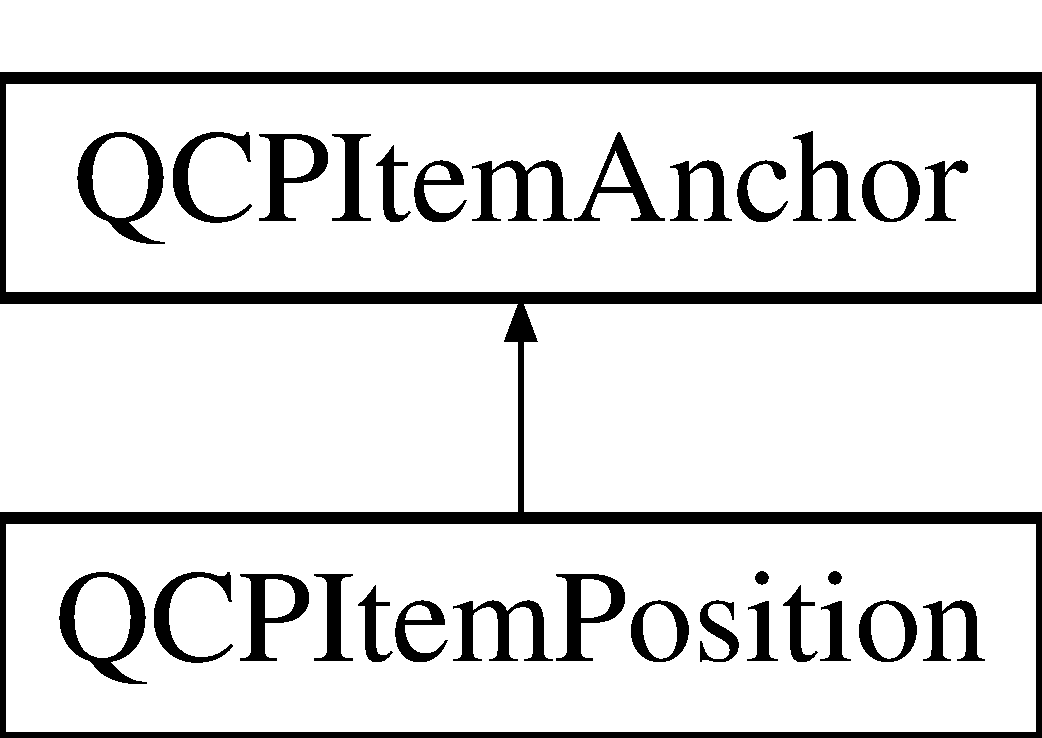
\includegraphics[height=2.000000cm]{class_q_c_p_item_position}
\end{center}
\end{figure}
\subsection*{Public Types}
\begin{DoxyCompactItemize}
\item 
enum \hyperlink{class_q_c_p_item_position_aad9936c22bf43e3d358552f6e86dbdc8}{Position\+Type} \{ \hyperlink{class_q_c_p_item_position_aad9936c22bf43e3d358552f6e86dbdc8a564f5e53e550ead1ec5fc7fc7d0b73e0}{pt\+Absolute}, 
\hyperlink{class_q_c_p_item_position_aad9936c22bf43e3d358552f6e86dbdc8ac7d6aa89ceacb39658b0d6da061c789a}{pt\+Viewport\+Ratio}, 
\hyperlink{class_q_c_p_item_position_aad9936c22bf43e3d358552f6e86dbdc8a01080fd00eaf09fa238ef6b73bbfef75}{pt\+Axis\+Rect\+Ratio}, 
\hyperlink{class_q_c_p_item_position_aad9936c22bf43e3d358552f6e86dbdc8ad5ffb8dc99ad73263f7010c77342294c}{pt\+Plot\+Coords}
 \}
\end{DoxyCompactItemize}
\subsection*{Public Member Functions}
\begin{DoxyCompactItemize}
\item 
\hyperlink{class_q_c_p_item_position_a3efc524f37fdcd22907545eb77555ce4}{Q\+C\+P\+Item\+Position} (\hyperlink{class_q_custom_plot}{Q\+Custom\+Plot} $\ast$parent\+Plot, \hyperlink{class_q_c_p_abstract_item}{Q\+C\+P\+Abstract\+Item} $\ast$parent\+Item, const Q\+String name)
\item 
\hyperlink{class_q_c_p_item_position_aad9936c22bf43e3d358552f6e86dbdc8}{Position\+Type} \hyperlink{class_q_c_p_item_position_abfd74d86bd799306ce0295ffe433bdfc}{type} () const
\item 
\hypertarget{class_q_c_p_item_position_a1415911868835701c04250566bfc681d}{}\label{class_q_c_p_item_position_a1415911868835701c04250566bfc681d} 
\hyperlink{class_q_c_p_item_position_aad9936c22bf43e3d358552f6e86dbdc8}{Position\+Type} {\bfseries typeX} () const
\item 
\hypertarget{class_q_c_p_item_position_ae47bac6f679c58f9e1c78dc63d56f331}{}\label{class_q_c_p_item_position_ae47bac6f679c58f9e1c78dc63d56f331} 
\hyperlink{class_q_c_p_item_position_aad9936c22bf43e3d358552f6e86dbdc8}{Position\+Type} {\bfseries typeY} () const
\item 
\hyperlink{class_q_c_p_item_anchor}{Q\+C\+P\+Item\+Anchor} $\ast$ \hyperlink{class_q_c_p_item_position_a0a87f9dce1af6cc9b510785991bcf1c6}{parent\+Anchor} () const
\item 
\hypertarget{class_q_c_p_item_position_a605cb8b2cf6044d3d03cb1a894faf98a}{}\label{class_q_c_p_item_position_a605cb8b2cf6044d3d03cb1a894faf98a} 
\hyperlink{class_q_c_p_item_anchor}{Q\+C\+P\+Item\+Anchor} $\ast$ {\bfseries parent\+AnchorX} () const
\item 
\hypertarget{class_q_c_p_item_position_aa40afec791a4339b09572922ca425ec2}{}\label{class_q_c_p_item_position_aa40afec791a4339b09572922ca425ec2} 
\hyperlink{class_q_c_p_item_anchor}{Q\+C\+P\+Item\+Anchor} $\ast$ {\bfseries parent\+AnchorY} () const
\item 
\hypertarget{class_q_c_p_item_position_a6fc519f1b73722a8d0cff7d4d647407e}{}\label{class_q_c_p_item_position_a6fc519f1b73722a8d0cff7d4d647407e} 
double {\bfseries key} () const
\item 
\hypertarget{class_q_c_p_item_position_acfcf86f840a7366a4299bff593d5d636}{}\label{class_q_c_p_item_position_acfcf86f840a7366a4299bff593d5d636} 
double {\bfseries value} () const
\item 
\hypertarget{class_q_c_p_item_position_aa4ecf5b04c67049c05d37619e090820b}{}\label{class_q_c_p_item_position_aa4ecf5b04c67049c05d37619e090820b} 
Q\+PointF {\bfseries coords} () const
\item 
\hypertarget{class_q_c_p_item_position_a9ad34861fbfd8be8b8270c16f879169c}{}\label{class_q_c_p_item_position_a9ad34861fbfd8be8b8270c16f879169c} 
\hyperlink{class_q_c_p_axis}{Q\+C\+P\+Axis} $\ast$ {\bfseries key\+Axis} () const
\item 
\hypertarget{class_q_c_p_item_position_a356ac94e7e73d88deb7f2841c0d0c734}{}\label{class_q_c_p_item_position_a356ac94e7e73d88deb7f2841c0d0c734} 
\hyperlink{class_q_c_p_axis}{Q\+C\+P\+Axis} $\ast$ {\bfseries value\+Axis} () const
\item 
\hypertarget{class_q_c_p_item_position_ae4081cfe7575f922f403c6e3a2ce7891}{}\label{class_q_c_p_item_position_ae4081cfe7575f922f403c6e3a2ce7891} 
\hyperlink{class_q_c_p_axis_rect}{Q\+C\+P\+Axis\+Rect} $\ast$ {\bfseries axis\+Rect} () const
\item 
virtual Q\+PointF \hyperlink{class_q_c_p_item_position_a6cad070c22801295231f5bd6045afe70}{pixel\+Point} () const
\item 
void \hyperlink{class_q_c_p_item_position_aa476abf71ed8fa4c537457ebb1a754ad}{set\+Type} (\hyperlink{class_q_c_p_item_position_aad9936c22bf43e3d358552f6e86dbdc8}{Position\+Type} \hyperlink{class_q_c_p_item_position_abfd74d86bd799306ce0295ffe433bdfc}{type})
\item 
void \hyperlink{class_q_c_p_item_position_a2113b2351d6d00457fb3559a4e20c3ea}{set\+TypeX} (\hyperlink{class_q_c_p_item_position_aad9936c22bf43e3d358552f6e86dbdc8}{Position\+Type} \hyperlink{class_q_c_p_item_position_abfd74d86bd799306ce0295ffe433bdfc}{type})
\item 
void \hyperlink{class_q_c_p_item_position_ac2a454aa5a54c1615c50686601ec4510}{set\+TypeY} (\hyperlink{class_q_c_p_item_position_aad9936c22bf43e3d358552f6e86dbdc8}{Position\+Type} \hyperlink{class_q_c_p_item_position_abfd74d86bd799306ce0295ffe433bdfc}{type})
\item 
bool \hyperlink{class_q_c_p_item_position_ac094d67a95d2dceafa0d50b9db3a7e51}{set\+Parent\+Anchor} (\hyperlink{class_q_c_p_item_anchor}{Q\+C\+P\+Item\+Anchor} $\ast$\hyperlink{class_q_c_p_item_position_a0a87f9dce1af6cc9b510785991bcf1c6}{parent\+Anchor}, bool keep\+Pixel\+Position=false)
\item 
bool \hyperlink{class_q_c_p_item_position_add71461a973927c74e42179480916d9c}{set\+Parent\+AnchorX} (\hyperlink{class_q_c_p_item_anchor}{Q\+C\+P\+Item\+Anchor} $\ast$\hyperlink{class_q_c_p_item_position_a0a87f9dce1af6cc9b510785991bcf1c6}{parent\+Anchor}, bool keep\+Pixel\+Position=false)
\item 
bool \hyperlink{class_q_c_p_item_position_add5ec1db9d19cec58a3b5c9e0a0c3f9d}{set\+Parent\+AnchorY} (\hyperlink{class_q_c_p_item_anchor}{Q\+C\+P\+Item\+Anchor} $\ast$\hyperlink{class_q_c_p_item_position_a0a87f9dce1af6cc9b510785991bcf1c6}{parent\+Anchor}, bool keep\+Pixel\+Position=false)
\item 
void \hyperlink{class_q_c_p_item_position_aa988ba4e87ab684c9021017dcaba945f}{set\+Coords} (double key, double value)
\item 
void \hyperlink{class_q_c_p_item_position_acc70b3abc143287f806e5f154e5e07b0}{set\+Coords} (const Q\+PointF \&coords)
\item 
void \hyperlink{class_q_c_p_item_position_a2185f45c75ac8cb9be89daeaaad50e37}{set\+Axes} (\hyperlink{class_q_c_p_axis}{Q\+C\+P\+Axis} $\ast$key\+Axis, \hyperlink{class_q_c_p_axis}{Q\+C\+P\+Axis} $\ast$value\+Axis)
\item 
void \hyperlink{class_q_c_p_item_position_a0cd9b326fb324710169e92e8ca0041c2}{set\+Axis\+Rect} (\hyperlink{class_q_c_p_axis_rect}{Q\+C\+P\+Axis\+Rect} $\ast$axis\+Rect)
\item 
void \hyperlink{class_q_c_p_item_position_ab404e56d9ac2ac2df0382c57933a71ef}{set\+Pixel\+Point} (const Q\+PointF \&\hyperlink{class_q_c_p_item_position_a6cad070c22801295231f5bd6045afe70}{pixel\+Point})
\end{DoxyCompactItemize}
\subsection*{Protected Member Functions}
\begin{DoxyCompactItemize}
\item 
virtual \hyperlink{class_q_c_p_item_position}{Q\+C\+P\+Item\+Position} $\ast$ \hyperlink{class_q_c_p_item_position_a577a7efc601df85a20b3e709d1ac320e}{to\+Q\+C\+P\+Item\+Position} ()
\end{DoxyCompactItemize}
\subsection*{Protected Attributes}
\begin{DoxyCompactItemize}
\item 
\hypertarget{class_q_c_p_item_position_ae2a617dce057c5f3ec6878c1823aa291}{}\label{class_q_c_p_item_position_ae2a617dce057c5f3ec6878c1823aa291} 
\hyperlink{class_q_c_p_item_position_aad9936c22bf43e3d358552f6e86dbdc8}{Position\+Type} {\bfseries m\+Position\+TypeX}
\item 
\hypertarget{class_q_c_p_item_position_a47c96c0ef4380e1af4aaa7c2265c260b}{}\label{class_q_c_p_item_position_a47c96c0ef4380e1af4aaa7c2265c260b} 
\hyperlink{class_q_c_p_item_position_aad9936c22bf43e3d358552f6e86dbdc8}{Position\+Type} {\bfseries m\+Position\+TypeY}
\item 
\hypertarget{class_q_c_p_item_position_a63967a33933231e92f68c8ce06bfc37e}{}\label{class_q_c_p_item_position_a63967a33933231e92f68c8ce06bfc37e} 
Q\+Pointer$<$ \hyperlink{class_q_c_p_axis}{Q\+C\+P\+Axis} $>$ {\bfseries m\+Key\+Axis}
\item 
\hypertarget{class_q_c_p_item_position_a505dc2da24ba274452c1c817fcaba011}{}\label{class_q_c_p_item_position_a505dc2da24ba274452c1c817fcaba011} 
Q\+Pointer$<$ \hyperlink{class_q_c_p_axis}{Q\+C\+P\+Axis} $>$ {\bfseries m\+Value\+Axis}
\item 
\hypertarget{class_q_c_p_item_position_add40fcb8994c247d85f42a126286b740}{}\label{class_q_c_p_item_position_add40fcb8994c247d85f42a126286b740} 
Q\+Pointer$<$ \hyperlink{class_q_c_p_axis_rect}{Q\+C\+P\+Axis\+Rect} $>$ {\bfseries m\+Axis\+Rect}
\item 
\hypertarget{class_q_c_p_item_position_a4ff3931ad115603dfb4c7000b24bb415}{}\label{class_q_c_p_item_position_a4ff3931ad115603dfb4c7000b24bb415} 
double {\bfseries m\+Key}
\item 
\hypertarget{class_q_c_p_item_position_a67bf5df69f587d53731724a7d61c6c3f}{}\label{class_q_c_p_item_position_a67bf5df69f587d53731724a7d61c6c3f} 
double {\bfseries m\+Value}
\item 
\hypertarget{class_q_c_p_item_position_a41b4641d18c90997b9c01bf304181bf0}{}\label{class_q_c_p_item_position_a41b4641d18c90997b9c01bf304181bf0} 
\hyperlink{class_q_c_p_item_anchor}{Q\+C\+P\+Item\+Anchor} $\ast$ {\bfseries m\+Parent\+AnchorX}
\item 
\hypertarget{class_q_c_p_item_position_afc6142a6a09c8fa41c44d3d54fadd737}{}\label{class_q_c_p_item_position_afc6142a6a09c8fa41c44d3d54fadd737} 
\hyperlink{class_q_c_p_item_anchor}{Q\+C\+P\+Item\+Anchor} $\ast$ {\bfseries m\+Parent\+AnchorY}
\end{DoxyCompactItemize}


\subsection{Detailed Description}
Manages the position of an item. 

Every item has at least one public \hyperlink{class_q_c_p_item_position}{Q\+C\+P\+Item\+Position} member pointer which provides ways to position the item on the \hyperlink{class_q_custom_plot}{Q\+Custom\+Plot} surface. Some items have multiple positions, for example \hyperlink{class_q_c_p_item_rect}{Q\+C\+P\+Item\+Rect} has two\+: {\itshape top\+Left} and {\itshape bottom\+Right}.

\hyperlink{class_q_c_p_item_position}{Q\+C\+P\+Item\+Position} has a type (\hyperlink{class_q_c_p_item_position_aad9936c22bf43e3d358552f6e86dbdc8}{Position\+Type}) that can be set with \hyperlink{class_q_c_p_item_position_aa476abf71ed8fa4c537457ebb1a754ad}{set\+Type}. This type defines how coordinates passed to \hyperlink{class_q_c_p_item_position_aa988ba4e87ab684c9021017dcaba945f}{set\+Coords} are to be interpreted, e.\+g. as absolute pixel coordinates, as plot coordinates of certain axes, etc. For more advanced plots it is also possible to assign different types per X/Y coordinate of the position (see \hyperlink{class_q_c_p_item_position_a2113b2351d6d00457fb3559a4e20c3ea}{set\+TypeX}, \hyperlink{class_q_c_p_item_position_ac2a454aa5a54c1615c50686601ec4510}{set\+TypeY}). This way an item could be positioned at a fixed pixel distance from the top in the Y direction, while following a plot coordinate in the X direction.

A \hyperlink{class_q_c_p_item_position}{Q\+C\+P\+Item\+Position} may have a parent \hyperlink{class_q_c_p_item_anchor}{Q\+C\+P\+Item\+Anchor}, see \hyperlink{class_q_c_p_item_position_ac094d67a95d2dceafa0d50b9db3a7e51}{set\+Parent\+Anchor}. This way you can tie multiple items together. If the \hyperlink{class_q_c_p_item_position}{Q\+C\+P\+Item\+Position} has a parent, its coordinates (\hyperlink{class_q_c_p_item_position_aa988ba4e87ab684c9021017dcaba945f}{set\+Coords}) are considered to be absolute pixels in the reference frame of the parent anchor, where (0, 0) means directly ontop of the parent anchor. For example, You could attach the {\itshape start} position of a \hyperlink{class_q_c_p_item_line}{Q\+C\+P\+Item\+Line} to the {\itshape bottom} anchor of a \hyperlink{class_q_c_p_item_text}{Q\+C\+P\+Item\+Text} to make the starting point of the line always be centered under the text label, no matter where the text is moved to. For more advanced plots, it is possible to assign different parent anchors per X/Y coordinate of the position, see \hyperlink{class_q_c_p_item_position_add71461a973927c74e42179480916d9c}{set\+Parent\+AnchorX}, \hyperlink{class_q_c_p_item_position_add5ec1db9d19cec58a3b5c9e0a0c3f9d}{set\+Parent\+AnchorY}. This way an item could follow another item in the X direction but stay at a fixed position in the Y direction. Or even follow item A in X, and item B in Y.

Note that every \hyperlink{class_q_c_p_item_position}{Q\+C\+P\+Item\+Position} inherits from \hyperlink{class_q_c_p_item_anchor}{Q\+C\+P\+Item\+Anchor} and thus can itself be used as parent anchor for other positions.

To set the apparent pixel position on the \hyperlink{class_q_custom_plot}{Q\+Custom\+Plot} surface directly, use \hyperlink{class_q_c_p_item_position_ab404e56d9ac2ac2df0382c57933a71ef}{set\+Pixel\+Point}. This works no matter what type this \hyperlink{class_q_c_p_item_position}{Q\+C\+P\+Item\+Position} is or what parent-\/child situation it is in, as \hyperlink{class_q_c_p_item_position_ab404e56d9ac2ac2df0382c57933a71ef}{set\+Pixel\+Point} transforms the coordinates appropriately, to make the position appear at the specified pixel values. 

\subsection{Member Enumeration Documentation}
\hypertarget{class_q_c_p_item_position_aad9936c22bf43e3d358552f6e86dbdc8}{}\label{class_q_c_p_item_position_aad9936c22bf43e3d358552f6e86dbdc8} 
\index{Q\+C\+P\+Item\+Position@{Q\+C\+P\+Item\+Position}!Position\+Type@{Position\+Type}}
\index{Position\+Type@{Position\+Type}!Q\+C\+P\+Item\+Position@{Q\+C\+P\+Item\+Position}}
\subsubsection{\texorpdfstring{Position\+Type}{PositionType}}
{\footnotesize\ttfamily enum \hyperlink{class_q_c_p_item_position_aad9936c22bf43e3d358552f6e86dbdc8}{Q\+C\+P\+Item\+Position\+::\+Position\+Type}}

Defines the ways an item position can be specified. Thus it defines what the numbers passed to \hyperlink{class_q_c_p_item_position_aa988ba4e87ab684c9021017dcaba945f}{set\+Coords} actually mean.

\begin{DoxySeeAlso}{See also}
\hyperlink{class_q_c_p_item_position_aa476abf71ed8fa4c537457ebb1a754ad}{set\+Type} 
\end{DoxySeeAlso}
\begin{DoxyEnumFields}{Enumerator}
\raisebox{\heightof{T}}[0pt][0pt]{\index{pt\+Absolute@{pt\+Absolute}!Q\+C\+P\+Item\+Position@{Q\+C\+P\+Item\+Position}}\index{Q\+C\+P\+Item\+Position@{Q\+C\+P\+Item\+Position}!pt\+Absolute@{pt\+Absolute}}}\hypertarget{class_q_c_p_item_position_aad9936c22bf43e3d358552f6e86dbdc8a564f5e53e550ead1ec5fc7fc7d0b73e0}{}\label{class_q_c_p_item_position_aad9936c22bf43e3d358552f6e86dbdc8a564f5e53e550ead1ec5fc7fc7d0b73e0} 
pt\+Absolute&Static positioning in pixels, starting from the top left corner of the viewport/widget. \\
\hline

\raisebox{\heightof{T}}[0pt][0pt]{\index{pt\+Viewport\+Ratio@{pt\+Viewport\+Ratio}!Q\+C\+P\+Item\+Position@{Q\+C\+P\+Item\+Position}}\index{Q\+C\+P\+Item\+Position@{Q\+C\+P\+Item\+Position}!pt\+Viewport\+Ratio@{pt\+Viewport\+Ratio}}}\hypertarget{class_q_c_p_item_position_aad9936c22bf43e3d358552f6e86dbdc8ac7d6aa89ceacb39658b0d6da061c789a}{}\label{class_q_c_p_item_position_aad9936c22bf43e3d358552f6e86dbdc8ac7d6aa89ceacb39658b0d6da061c789a} 
pt\+Viewport\+Ratio&Static positioning given by a fraction of the viewport size. For example, if you call set\+Coords(0, 0), the position will be at the top left corner of the viewport/widget. set\+Coords(1, 1) will be at the bottom right corner, set\+Coords(0.\+5, 0) will be horizontally centered and vertically at the top of the viewport/widget, etc. \\
\hline

\raisebox{\heightof{T}}[0pt][0pt]{\index{pt\+Axis\+Rect\+Ratio@{pt\+Axis\+Rect\+Ratio}!Q\+C\+P\+Item\+Position@{Q\+C\+P\+Item\+Position}}\index{Q\+C\+P\+Item\+Position@{Q\+C\+P\+Item\+Position}!pt\+Axis\+Rect\+Ratio@{pt\+Axis\+Rect\+Ratio}}}\hypertarget{class_q_c_p_item_position_aad9936c22bf43e3d358552f6e86dbdc8a01080fd00eaf09fa238ef6b73bbfef75}{}\label{class_q_c_p_item_position_aad9936c22bf43e3d358552f6e86dbdc8a01080fd00eaf09fa238ef6b73bbfef75} 
pt\+Axis\+Rect\+Ratio&Static positioning given by a fraction of the axis rect size (see \hyperlink{class_q_c_p_item_position_a0cd9b326fb324710169e92e8ca0041c2}{set\+Axis\+Rect}). For example, if you call set\+Coords(0, 0), the position will be at the top left corner of the axis rect. set\+Coords(1, 1) will be at the bottom right corner, set\+Coords(0.\+5, 0) will be horizontally centered and vertically at the top of the axis rect, etc. You can also go beyond the axis rect by providing negative coordinates or coordinates larger than 1. \\
\hline

\raisebox{\heightof{T}}[0pt][0pt]{\index{pt\+Plot\+Coords@{pt\+Plot\+Coords}!Q\+C\+P\+Item\+Position@{Q\+C\+P\+Item\+Position}}\index{Q\+C\+P\+Item\+Position@{Q\+C\+P\+Item\+Position}!pt\+Plot\+Coords@{pt\+Plot\+Coords}}}\hypertarget{class_q_c_p_item_position_aad9936c22bf43e3d358552f6e86dbdc8ad5ffb8dc99ad73263f7010c77342294c}{}\label{class_q_c_p_item_position_aad9936c22bf43e3d358552f6e86dbdc8ad5ffb8dc99ad73263f7010c77342294c} 
pt\+Plot\+Coords&Dynamic positioning at a plot coordinate defined by two axes (see \hyperlink{class_q_c_p_item_position_a2185f45c75ac8cb9be89daeaaad50e37}{set\+Axes}). \\
\hline

\end{DoxyEnumFields}


\subsection{Constructor \& Destructor Documentation}
\hypertarget{class_q_c_p_item_position_a3efc524f37fdcd22907545eb77555ce4}{}\label{class_q_c_p_item_position_a3efc524f37fdcd22907545eb77555ce4} 
\index{Q\+C\+P\+Item\+Position@{Q\+C\+P\+Item\+Position}!Q\+C\+P\+Item\+Position@{Q\+C\+P\+Item\+Position}}
\index{Q\+C\+P\+Item\+Position@{Q\+C\+P\+Item\+Position}!Q\+C\+P\+Item\+Position@{Q\+C\+P\+Item\+Position}}
\subsubsection{\texorpdfstring{Q\+C\+P\+Item\+Position()}{QCPItemPosition()}}
{\footnotesize\ttfamily Q\+C\+P\+Item\+Position\+::\+Q\+C\+P\+Item\+Position (\begin{DoxyParamCaption}\item[{\hyperlink{class_q_custom_plot}{Q\+Custom\+Plot} $\ast$}]{parent\+Plot,  }\item[{\hyperlink{class_q_c_p_abstract_item}{Q\+C\+P\+Abstract\+Item} $\ast$}]{parent\+Item,  }\item[{const Q\+String}]{name }\end{DoxyParamCaption})}

Creates a new \hyperlink{class_q_c_p_item_position}{Q\+C\+P\+Item\+Position}. You shouldn\textquotesingle{}t create \hyperlink{class_q_c_p_item_position}{Q\+C\+P\+Item\+Position} instances directly, even if you want to make a new item subclass. Use Q\+C\+P\+Abstract\+Item\+::create\+Position instead, as explained in the subclassing section of the \hyperlink{class_q_c_p_abstract_item}{Q\+C\+P\+Abstract\+Item} documentation. 

\subsection{Member Function Documentation}
\hypertarget{class_q_c_p_item_position_a0a87f9dce1af6cc9b510785991bcf1c6}{}\label{class_q_c_p_item_position_a0a87f9dce1af6cc9b510785991bcf1c6} 
\index{Q\+C\+P\+Item\+Position@{Q\+C\+P\+Item\+Position}!parent\+Anchor@{parent\+Anchor}}
\index{parent\+Anchor@{parent\+Anchor}!Q\+C\+P\+Item\+Position@{Q\+C\+P\+Item\+Position}}
\subsubsection{\texorpdfstring{parent\+Anchor()}{parentAnchor()}}
{\footnotesize\ttfamily \hyperlink{class_q_c_p_item_anchor}{Q\+C\+P\+Item\+Anchor} $\ast$ Q\+C\+P\+Item\+Position\+::parent\+Anchor (\begin{DoxyParamCaption}{ }\end{DoxyParamCaption}) const\hspace{0.3cm}{\ttfamily [inline]}}

Returns the current parent anchor.

If different parent anchors were set for X and Y (\hyperlink{class_q_c_p_item_position_add71461a973927c74e42179480916d9c}{set\+Parent\+AnchorX}, \hyperlink{class_q_c_p_item_position_add5ec1db9d19cec58a3b5c9e0a0c3f9d}{set\+Parent\+AnchorY}), this method returns the parent anchor of the Y coordinate. In that case rather use {\itshape parent\+Anchor\+X()} and {\itshape parent\+Anchor\+Y()}.

\begin{DoxySeeAlso}{See also}
\hyperlink{class_q_c_p_item_position_ac094d67a95d2dceafa0d50b9db3a7e51}{set\+Parent\+Anchor} 
\end{DoxySeeAlso}
\hypertarget{class_q_c_p_item_position_a6cad070c22801295231f5bd6045afe70}{}\label{class_q_c_p_item_position_a6cad070c22801295231f5bd6045afe70} 
\index{Q\+C\+P\+Item\+Position@{Q\+C\+P\+Item\+Position}!pixel\+Point@{pixel\+Point}}
\index{pixel\+Point@{pixel\+Point}!Q\+C\+P\+Item\+Position@{Q\+C\+P\+Item\+Position}}
\subsubsection{\texorpdfstring{pixel\+Point()}{pixelPoint()}}
{\footnotesize\ttfamily Q\+PointF Q\+C\+P\+Item\+Position\+::pixel\+Point (\begin{DoxyParamCaption}{ }\end{DoxyParamCaption}) const\hspace{0.3cm}{\ttfamily [virtual]}}

Returns the final absolute pixel position of the \hyperlink{class_q_c_p_item_position}{Q\+C\+P\+Item\+Position} on the \hyperlink{class_q_custom_plot}{Q\+Custom\+Plot} surface. It includes all effects of type (\hyperlink{class_q_c_p_item_position_aa476abf71ed8fa4c537457ebb1a754ad}{set\+Type}) and possible parent anchors (\hyperlink{class_q_c_p_item_position_ac094d67a95d2dceafa0d50b9db3a7e51}{set\+Parent\+Anchor}).

\begin{DoxySeeAlso}{See also}
\hyperlink{class_q_c_p_item_position_ab404e56d9ac2ac2df0382c57933a71ef}{set\+Pixel\+Point} 
\end{DoxySeeAlso}


Reimplemented from \hyperlink{class_q_c_p_item_anchor_ae1a21d9471d1d788624cad297e1b8d6f}{Q\+C\+P\+Item\+Anchor}.

\hypertarget{class_q_c_p_item_position_a2185f45c75ac8cb9be89daeaaad50e37}{}\label{class_q_c_p_item_position_a2185f45c75ac8cb9be89daeaaad50e37} 
\index{Q\+C\+P\+Item\+Position@{Q\+C\+P\+Item\+Position}!set\+Axes@{set\+Axes}}
\index{set\+Axes@{set\+Axes}!Q\+C\+P\+Item\+Position@{Q\+C\+P\+Item\+Position}}
\subsubsection{\texorpdfstring{set\+Axes()}{setAxes()}}
{\footnotesize\ttfamily void Q\+C\+P\+Item\+Position\+::set\+Axes (\begin{DoxyParamCaption}\item[{\hyperlink{class_q_c_p_axis}{Q\+C\+P\+Axis} $\ast$}]{key\+Axis,  }\item[{\hyperlink{class_q_c_p_axis}{Q\+C\+P\+Axis} $\ast$}]{value\+Axis }\end{DoxyParamCaption})}

When \hyperlink{class_q_c_p_item_position_aa476abf71ed8fa4c537457ebb1a754ad}{set\+Type} is \hyperlink{class_q_c_p_item_position_aad9936c22bf43e3d358552f6e86dbdc8ad5ffb8dc99ad73263f7010c77342294c}{pt\+Plot\+Coords}, this function may be used to specify the axes the coordinates set with \hyperlink{class_q_c_p_item_position_aa988ba4e87ab684c9021017dcaba945f}{set\+Coords} relate to. By default they are set to the initial x\+Axis and y\+Axis of the \hyperlink{class_q_custom_plot}{Q\+Custom\+Plot}. \hypertarget{class_q_c_p_item_position_a0cd9b326fb324710169e92e8ca0041c2}{}\label{class_q_c_p_item_position_a0cd9b326fb324710169e92e8ca0041c2} 
\index{Q\+C\+P\+Item\+Position@{Q\+C\+P\+Item\+Position}!set\+Axis\+Rect@{set\+Axis\+Rect}}
\index{set\+Axis\+Rect@{set\+Axis\+Rect}!Q\+C\+P\+Item\+Position@{Q\+C\+P\+Item\+Position}}
\subsubsection{\texorpdfstring{set\+Axis\+Rect()}{setAxisRect()}}
{\footnotesize\ttfamily void Q\+C\+P\+Item\+Position\+::set\+Axis\+Rect (\begin{DoxyParamCaption}\item[{\hyperlink{class_q_c_p_axis_rect}{Q\+C\+P\+Axis\+Rect} $\ast$}]{axis\+Rect }\end{DoxyParamCaption})}

When \hyperlink{class_q_c_p_item_position_aa476abf71ed8fa4c537457ebb1a754ad}{set\+Type} is \hyperlink{class_q_c_p_item_position_aad9936c22bf43e3d358552f6e86dbdc8a01080fd00eaf09fa238ef6b73bbfef75}{pt\+Axis\+Rect\+Ratio}, this function may be used to specify the axis rect the coordinates set with \hyperlink{class_q_c_p_item_position_aa988ba4e87ab684c9021017dcaba945f}{set\+Coords} relate to. By default this is set to the main axis rect of the \hyperlink{class_q_custom_plot}{Q\+Custom\+Plot}. \hypertarget{class_q_c_p_item_position_aa988ba4e87ab684c9021017dcaba945f}{}\label{class_q_c_p_item_position_aa988ba4e87ab684c9021017dcaba945f} 
\index{Q\+C\+P\+Item\+Position@{Q\+C\+P\+Item\+Position}!set\+Coords@{set\+Coords}}
\index{set\+Coords@{set\+Coords}!Q\+C\+P\+Item\+Position@{Q\+C\+P\+Item\+Position}}
\subsubsection{\texorpdfstring{set\+Coords()}{setCoords()}\hspace{0.1cm}{\footnotesize\ttfamily [1/2]}}
{\footnotesize\ttfamily void Q\+C\+P\+Item\+Position\+::set\+Coords (\begin{DoxyParamCaption}\item[{double}]{key,  }\item[{double}]{value }\end{DoxyParamCaption})}

Sets the coordinates of this \hyperlink{class_q_c_p_item_position}{Q\+C\+P\+Item\+Position}. What the coordinates mean, is defined by the type (\hyperlink{class_q_c_p_item_position_aa476abf71ed8fa4c537457ebb1a754ad}{set\+Type}, \hyperlink{class_q_c_p_item_position_a2113b2351d6d00457fb3559a4e20c3ea}{set\+TypeX}, \hyperlink{class_q_c_p_item_position_ac2a454aa5a54c1615c50686601ec4510}{set\+TypeY}).

For example, if the type is \hyperlink{class_q_c_p_item_position_aad9936c22bf43e3d358552f6e86dbdc8a564f5e53e550ead1ec5fc7fc7d0b73e0}{pt\+Absolute}, {\itshape key} and {\itshape value} mean the x and y pixel position on the \hyperlink{class_q_custom_plot}{Q\+Custom\+Plot} surface. In that case the origin (0, 0) is in the top left corner of the \hyperlink{class_q_custom_plot}{Q\+Custom\+Plot} viewport. If the type is \hyperlink{class_q_c_p_item_position_aad9936c22bf43e3d358552f6e86dbdc8ad5ffb8dc99ad73263f7010c77342294c}{pt\+Plot\+Coords}, {\itshape key} and {\itshape value} mean a point in the plot coordinate system defined by the axes set by \hyperlink{class_q_c_p_item_position_a2185f45c75ac8cb9be89daeaaad50e37}{set\+Axes}. By default those are the \hyperlink{class_q_custom_plot}{Q\+Custom\+Plot}\textquotesingle{}s x\+Axis and y\+Axis. See the documentation of \hyperlink{class_q_c_p_item_position_aa476abf71ed8fa4c537457ebb1a754ad}{set\+Type} for other available coordinate types and their meaning.

If different types were configured for X and Y (\hyperlink{class_q_c_p_item_position_a2113b2351d6d00457fb3559a4e20c3ea}{set\+TypeX}, \hyperlink{class_q_c_p_item_position_ac2a454aa5a54c1615c50686601ec4510}{set\+TypeY}), {\itshape key} and {\itshape value} must also be provided in the different coordinate systems. Here, the X type refers to {\itshape key}, and the Y type refers to {\itshape value}.

\begin{DoxySeeAlso}{See also}
\hyperlink{class_q_c_p_item_position_ab404e56d9ac2ac2df0382c57933a71ef}{set\+Pixel\+Point} 
\end{DoxySeeAlso}
\hypertarget{class_q_c_p_item_position_acc70b3abc143287f806e5f154e5e07b0}{}\label{class_q_c_p_item_position_acc70b3abc143287f806e5f154e5e07b0} 
\index{Q\+C\+P\+Item\+Position@{Q\+C\+P\+Item\+Position}!set\+Coords@{set\+Coords}}
\index{set\+Coords@{set\+Coords}!Q\+C\+P\+Item\+Position@{Q\+C\+P\+Item\+Position}}
\subsubsection{\texorpdfstring{set\+Coords()}{setCoords()}\hspace{0.1cm}{\footnotesize\ttfamily [2/2]}}
{\footnotesize\ttfamily void Q\+C\+P\+Item\+Position\+::set\+Coords (\begin{DoxyParamCaption}\item[{const Q\+PointF \&}]{pos }\end{DoxyParamCaption})}

This is an overloaded member function, provided for convenience. It differs from the above function only in what argument(s) it accepts.

Sets the coordinates as a Q\+PointF {\itshape pos} where pos.\+x has the meaning of {\itshape key} and pos.\+y the meaning of {\itshape value} of the \hyperlink{class_q_c_p_item_position_aa988ba4e87ab684c9021017dcaba945f}{set\+Coords(double key, double value)} method. \hypertarget{class_q_c_p_item_position_ac094d67a95d2dceafa0d50b9db3a7e51}{}\label{class_q_c_p_item_position_ac094d67a95d2dceafa0d50b9db3a7e51} 
\index{Q\+C\+P\+Item\+Position@{Q\+C\+P\+Item\+Position}!set\+Parent\+Anchor@{set\+Parent\+Anchor}}
\index{set\+Parent\+Anchor@{set\+Parent\+Anchor}!Q\+C\+P\+Item\+Position@{Q\+C\+P\+Item\+Position}}
\subsubsection{\texorpdfstring{set\+Parent\+Anchor()}{setParentAnchor()}}
{\footnotesize\ttfamily bool Q\+C\+P\+Item\+Position\+::set\+Parent\+Anchor (\begin{DoxyParamCaption}\item[{\hyperlink{class_q_c_p_item_anchor}{Q\+C\+P\+Item\+Anchor} $\ast$}]{parent\+Anchor,  }\item[{bool}]{keep\+Pixel\+Position = {\ttfamily false} }\end{DoxyParamCaption})}

Sets the parent of this \hyperlink{class_q_c_p_item_position}{Q\+C\+P\+Item\+Position} to {\itshape parent\+Anchor}. This means the position will now follow any position changes of the anchor. The local coordinate system of positions with a parent anchor always is absolute pixels, with (0, 0) being exactly on top of the parent anchor. (Hence the type shouldn\textquotesingle{}t be set to \hyperlink{class_q_c_p_item_position_aad9936c22bf43e3d358552f6e86dbdc8ad5ffb8dc99ad73263f7010c77342294c}{pt\+Plot\+Coords} for positions with parent anchors.)

if {\itshape keep\+Pixel\+Position} is true, the current pixel position of the \hyperlink{class_q_c_p_item_position}{Q\+C\+P\+Item\+Position} is preserved during reparenting. If it\textquotesingle{}s set to false, the coordinates are set to (0, 0), i.\+e. the position will be exactly on top of the parent anchor.

To remove this \hyperlink{class_q_c_p_item_position}{Q\+C\+P\+Item\+Position} from any parent anchor, set {\itshape parent\+Anchor} to 0.

If the \hyperlink{class_q_c_p_item_position}{Q\+C\+P\+Item\+Position} previously had no parent and the type is \hyperlink{class_q_c_p_item_position_aad9936c22bf43e3d358552f6e86dbdc8ad5ffb8dc99ad73263f7010c77342294c}{pt\+Plot\+Coords}, the type is set to \hyperlink{class_q_c_p_item_position_aad9936c22bf43e3d358552f6e86dbdc8a564f5e53e550ead1ec5fc7fc7d0b73e0}{pt\+Absolute}, to keep the position in a valid state.

This method sets the parent anchor for both X and Y directions. It is also possible to set different parents for X and Y, see \hyperlink{class_q_c_p_item_position_add71461a973927c74e42179480916d9c}{set\+Parent\+AnchorX}, \hyperlink{class_q_c_p_item_position_add5ec1db9d19cec58a3b5c9e0a0c3f9d}{set\+Parent\+AnchorY}. \hypertarget{class_q_c_p_item_position_add71461a973927c74e42179480916d9c}{}\label{class_q_c_p_item_position_add71461a973927c74e42179480916d9c} 
\index{Q\+C\+P\+Item\+Position@{Q\+C\+P\+Item\+Position}!set\+Parent\+AnchorX@{set\+Parent\+AnchorX}}
\index{set\+Parent\+AnchorX@{set\+Parent\+AnchorX}!Q\+C\+P\+Item\+Position@{Q\+C\+P\+Item\+Position}}
\subsubsection{\texorpdfstring{set\+Parent\+Anchor\+X()}{setParentAnchorX()}}
{\footnotesize\ttfamily bool Q\+C\+P\+Item\+Position\+::set\+Parent\+AnchorX (\begin{DoxyParamCaption}\item[{\hyperlink{class_q_c_p_item_anchor}{Q\+C\+P\+Item\+Anchor} $\ast$}]{parent\+Anchor,  }\item[{bool}]{keep\+Pixel\+Position = {\ttfamily false} }\end{DoxyParamCaption})}

This method sets the parent anchor of the X coordinate to {\itshape parent\+Anchor}.

For a detailed description of what a parent anchor is, see the documentation of \hyperlink{class_q_c_p_item_position_ac094d67a95d2dceafa0d50b9db3a7e51}{set\+Parent\+Anchor}.

\begin{DoxySeeAlso}{See also}
\hyperlink{class_q_c_p_item_position_ac094d67a95d2dceafa0d50b9db3a7e51}{set\+Parent\+Anchor}, \hyperlink{class_q_c_p_item_position_add5ec1db9d19cec58a3b5c9e0a0c3f9d}{set\+Parent\+AnchorY} 
\end{DoxySeeAlso}
\hypertarget{class_q_c_p_item_position_add5ec1db9d19cec58a3b5c9e0a0c3f9d}{}\label{class_q_c_p_item_position_add5ec1db9d19cec58a3b5c9e0a0c3f9d} 
\index{Q\+C\+P\+Item\+Position@{Q\+C\+P\+Item\+Position}!set\+Parent\+AnchorY@{set\+Parent\+AnchorY}}
\index{set\+Parent\+AnchorY@{set\+Parent\+AnchorY}!Q\+C\+P\+Item\+Position@{Q\+C\+P\+Item\+Position}}
\subsubsection{\texorpdfstring{set\+Parent\+Anchor\+Y()}{setParentAnchorY()}}
{\footnotesize\ttfamily bool Q\+C\+P\+Item\+Position\+::set\+Parent\+AnchorY (\begin{DoxyParamCaption}\item[{\hyperlink{class_q_c_p_item_anchor}{Q\+C\+P\+Item\+Anchor} $\ast$}]{parent\+Anchor,  }\item[{bool}]{keep\+Pixel\+Position = {\ttfamily false} }\end{DoxyParamCaption})}

This method sets the parent anchor of the Y coordinate to {\itshape parent\+Anchor}.

For a detailed description of what a parent anchor is, see the documentation of \hyperlink{class_q_c_p_item_position_ac094d67a95d2dceafa0d50b9db3a7e51}{set\+Parent\+Anchor}.

\begin{DoxySeeAlso}{See also}
\hyperlink{class_q_c_p_item_position_ac094d67a95d2dceafa0d50b9db3a7e51}{set\+Parent\+Anchor}, \hyperlink{class_q_c_p_item_position_add71461a973927c74e42179480916d9c}{set\+Parent\+AnchorX} 
\end{DoxySeeAlso}
\hypertarget{class_q_c_p_item_position_ab404e56d9ac2ac2df0382c57933a71ef}{}\label{class_q_c_p_item_position_ab404e56d9ac2ac2df0382c57933a71ef} 
\index{Q\+C\+P\+Item\+Position@{Q\+C\+P\+Item\+Position}!set\+Pixel\+Point@{set\+Pixel\+Point}}
\index{set\+Pixel\+Point@{set\+Pixel\+Point}!Q\+C\+P\+Item\+Position@{Q\+C\+P\+Item\+Position}}
\subsubsection{\texorpdfstring{set\+Pixel\+Point()}{setPixelPoint()}}
{\footnotesize\ttfamily void Q\+C\+P\+Item\+Position\+::set\+Pixel\+Point (\begin{DoxyParamCaption}\item[{const Q\+PointF \&}]{pixel\+Point }\end{DoxyParamCaption})}

Sets the apparent pixel position. This works no matter what type (\hyperlink{class_q_c_p_item_position_aa476abf71ed8fa4c537457ebb1a754ad}{set\+Type}) this \hyperlink{class_q_c_p_item_position}{Q\+C\+P\+Item\+Position} is or what parent-\/child situation it is in, as coordinates are transformed appropriately, to make the position finally appear at the specified pixel values.

Only if the type is \hyperlink{class_q_c_p_item_position_aad9936c22bf43e3d358552f6e86dbdc8a564f5e53e550ead1ec5fc7fc7d0b73e0}{pt\+Absolute} and no parent anchor is set, this function\textquotesingle{}s effect is identical to that of \hyperlink{class_q_c_p_item_position_aa988ba4e87ab684c9021017dcaba945f}{set\+Coords}.

\begin{DoxySeeAlso}{See also}
\hyperlink{class_q_c_p_item_position_a6cad070c22801295231f5bd6045afe70}{pixel\+Point}, \hyperlink{class_q_c_p_item_position_aa988ba4e87ab684c9021017dcaba945f}{set\+Coords} 
\end{DoxySeeAlso}
\hypertarget{class_q_c_p_item_position_aa476abf71ed8fa4c537457ebb1a754ad}{}\label{class_q_c_p_item_position_aa476abf71ed8fa4c537457ebb1a754ad} 
\index{Q\+C\+P\+Item\+Position@{Q\+C\+P\+Item\+Position}!set\+Type@{set\+Type}}
\index{set\+Type@{set\+Type}!Q\+C\+P\+Item\+Position@{Q\+C\+P\+Item\+Position}}
\subsubsection{\texorpdfstring{set\+Type()}{setType()}}
{\footnotesize\ttfamily void Q\+C\+P\+Item\+Position\+::set\+Type (\begin{DoxyParamCaption}\item[{\hyperlink{class_q_c_p_item_position_aad9936c22bf43e3d358552f6e86dbdc8}{Q\+C\+P\+Item\+Position\+::\+Position\+Type}}]{type }\end{DoxyParamCaption})}

Sets the type of the position. The type defines how the coordinates passed to \hyperlink{class_q_c_p_item_position_aa988ba4e87ab684c9021017dcaba945f}{set\+Coords} should be handled and how the \hyperlink{class_q_c_p_item_position}{Q\+C\+P\+Item\+Position} should behave in the plot.

The possible values for {\itshape type} can be separated in two main categories\+:

\begin{DoxyItemize}
\item The position is regarded as a point in plot coordinates. This corresponds to \hyperlink{class_q_c_p_item_position_aad9936c22bf43e3d358552f6e86dbdc8ad5ffb8dc99ad73263f7010c77342294c}{pt\+Plot\+Coords} and requires two axes that define the plot coordinate system. They can be specified with \hyperlink{class_q_c_p_item_position_a2185f45c75ac8cb9be89daeaaad50e37}{set\+Axes}. By default, the \hyperlink{class_q_custom_plot}{Q\+Custom\+Plot}\textquotesingle{}s x-\/ and y\+Axis are used.\end{DoxyItemize}
\begin{DoxyItemize}
\item The position is fixed on the \hyperlink{class_q_custom_plot}{Q\+Custom\+Plot} surface, i.\+e. independent of axis ranges. This corresponds to all other types, i.\+e. \hyperlink{class_q_c_p_item_position_aad9936c22bf43e3d358552f6e86dbdc8a564f5e53e550ead1ec5fc7fc7d0b73e0}{pt\+Absolute}, \hyperlink{class_q_c_p_item_position_aad9936c22bf43e3d358552f6e86dbdc8ac7d6aa89ceacb39658b0d6da061c789a}{pt\+Viewport\+Ratio} and \hyperlink{class_q_c_p_item_position_aad9936c22bf43e3d358552f6e86dbdc8a01080fd00eaf09fa238ef6b73bbfef75}{pt\+Axis\+Rect\+Ratio}. They differ only in the way the absolute position is described, see the documentation of \hyperlink{class_q_c_p_item_position_aad9936c22bf43e3d358552f6e86dbdc8}{Position\+Type} for details. For \hyperlink{class_q_c_p_item_position_aad9936c22bf43e3d358552f6e86dbdc8a01080fd00eaf09fa238ef6b73bbfef75}{pt\+Axis\+Rect\+Ratio}, note that you can specify the axis rect with \hyperlink{class_q_c_p_item_position_a0cd9b326fb324710169e92e8ca0041c2}{set\+Axis\+Rect}. By default this is set to the main axis rect.\end{DoxyItemize}
Note that the position type \hyperlink{class_q_c_p_item_position_aad9936c22bf43e3d358552f6e86dbdc8ad5ffb8dc99ad73263f7010c77342294c}{pt\+Plot\+Coords} is only available (and sensible) when the position has no parent anchor (\hyperlink{class_q_c_p_item_position_ac094d67a95d2dceafa0d50b9db3a7e51}{set\+Parent\+Anchor}).

If the type is changed, the apparent pixel position on the plot is preserved. This means the coordinates as retrieved with coords() and set with \hyperlink{class_q_c_p_item_position_aa988ba4e87ab684c9021017dcaba945f}{set\+Coords} may change in the process.

This method sets the type for both X and Y directions. It is also possible to set different types for X and Y, see \hyperlink{class_q_c_p_item_position_a2113b2351d6d00457fb3559a4e20c3ea}{set\+TypeX}, \hyperlink{class_q_c_p_item_position_ac2a454aa5a54c1615c50686601ec4510}{set\+TypeY}. \hypertarget{class_q_c_p_item_position_a2113b2351d6d00457fb3559a4e20c3ea}{}\label{class_q_c_p_item_position_a2113b2351d6d00457fb3559a4e20c3ea} 
\index{Q\+C\+P\+Item\+Position@{Q\+C\+P\+Item\+Position}!set\+TypeX@{set\+TypeX}}
\index{set\+TypeX@{set\+TypeX}!Q\+C\+P\+Item\+Position@{Q\+C\+P\+Item\+Position}}
\subsubsection{\texorpdfstring{set\+Type\+X()}{setTypeX()}}
{\footnotesize\ttfamily void Q\+C\+P\+Item\+Position\+::set\+TypeX (\begin{DoxyParamCaption}\item[{\hyperlink{class_q_c_p_item_position_aad9936c22bf43e3d358552f6e86dbdc8}{Q\+C\+P\+Item\+Position\+::\+Position\+Type}}]{type }\end{DoxyParamCaption})}

This method sets the position type of the X coordinate to {\itshape type}.

For a detailed description of what a position type is, see the documentation of \hyperlink{class_q_c_p_item_position_aa476abf71ed8fa4c537457ebb1a754ad}{set\+Type}.

\begin{DoxySeeAlso}{See also}
\hyperlink{class_q_c_p_item_position_aa476abf71ed8fa4c537457ebb1a754ad}{set\+Type}, \hyperlink{class_q_c_p_item_position_ac2a454aa5a54c1615c50686601ec4510}{set\+TypeY} 
\end{DoxySeeAlso}
\hypertarget{class_q_c_p_item_position_ac2a454aa5a54c1615c50686601ec4510}{}\label{class_q_c_p_item_position_ac2a454aa5a54c1615c50686601ec4510} 
\index{Q\+C\+P\+Item\+Position@{Q\+C\+P\+Item\+Position}!set\+TypeY@{set\+TypeY}}
\index{set\+TypeY@{set\+TypeY}!Q\+C\+P\+Item\+Position@{Q\+C\+P\+Item\+Position}}
\subsubsection{\texorpdfstring{set\+Type\+Y()}{setTypeY()}}
{\footnotesize\ttfamily void Q\+C\+P\+Item\+Position\+::set\+TypeY (\begin{DoxyParamCaption}\item[{\hyperlink{class_q_c_p_item_position_aad9936c22bf43e3d358552f6e86dbdc8}{Q\+C\+P\+Item\+Position\+::\+Position\+Type}}]{type }\end{DoxyParamCaption})}

This method sets the position type of the Y coordinate to {\itshape type}.

For a detailed description of what a position type is, see the documentation of \hyperlink{class_q_c_p_item_position_aa476abf71ed8fa4c537457ebb1a754ad}{set\+Type}.

\begin{DoxySeeAlso}{See also}
\hyperlink{class_q_c_p_item_position_aa476abf71ed8fa4c537457ebb1a754ad}{set\+Type}, \hyperlink{class_q_c_p_item_position_a2113b2351d6d00457fb3559a4e20c3ea}{set\+TypeX} 
\end{DoxySeeAlso}
\hypertarget{class_q_c_p_item_position_a577a7efc601df85a20b3e709d1ac320e}{}\label{class_q_c_p_item_position_a577a7efc601df85a20b3e709d1ac320e} 
\index{Q\+C\+P\+Item\+Position@{Q\+C\+P\+Item\+Position}!to\+Q\+C\+P\+Item\+Position@{to\+Q\+C\+P\+Item\+Position}}
\index{to\+Q\+C\+P\+Item\+Position@{to\+Q\+C\+P\+Item\+Position}!Q\+C\+P\+Item\+Position@{Q\+C\+P\+Item\+Position}}
\subsubsection{\texorpdfstring{to\+Q\+C\+P\+Item\+Position()}{toQCPItemPosition()}}
{\footnotesize\ttfamily virtual \hyperlink{class_q_c_p_item_position}{Q\+C\+P\+Item\+Position}$\ast$ Q\+C\+P\+Item\+Position\+::to\+Q\+C\+P\+Item\+Position (\begin{DoxyParamCaption}{ }\end{DoxyParamCaption})\hspace{0.3cm}{\ttfamily [inline]}, {\ttfamily [protected]}, {\ttfamily [virtual]}}

Returns 0 if this instance is merely a \hyperlink{class_q_c_p_item_anchor}{Q\+C\+P\+Item\+Anchor}, and a valid pointer of type Q\+C\+P\+Item\+Position$\ast$ if it actually is a \hyperlink{class_q_c_p_item_position}{Q\+C\+P\+Item\+Position} (which is a subclass of \hyperlink{class_q_c_p_item_anchor}{Q\+C\+P\+Item\+Anchor}).

This safe downcast functionality could also be achieved with a dynamic\+\_\+cast. However, \hyperlink{class_q_custom_plot}{Q\+Custom\+Plot} avoids dynamic\+\_\+cast to work with projects that don\textquotesingle{}t have R\+T\+TI support enabled (e.\+g. -\/fno-\/rtti flag with gcc compiler). 

Reimplemented from \hyperlink{class_q_c_p_item_anchor_ac54b20120669950255a63587193dbb86}{Q\+C\+P\+Item\+Anchor}.

\hypertarget{class_q_c_p_item_position_abfd74d86bd799306ce0295ffe433bdfc}{}\label{class_q_c_p_item_position_abfd74d86bd799306ce0295ffe433bdfc} 
\index{Q\+C\+P\+Item\+Position@{Q\+C\+P\+Item\+Position}!type@{type}}
\index{type@{type}!Q\+C\+P\+Item\+Position@{Q\+C\+P\+Item\+Position}}
\subsubsection{\texorpdfstring{type()}{type()}}
{\footnotesize\ttfamily \hyperlink{class_q_c_p_item_position_aad9936c22bf43e3d358552f6e86dbdc8}{Q\+C\+P\+Item\+Position\+::\+Position\+Type} $\ast$ Q\+C\+P\+Item\+Position\+::type (\begin{DoxyParamCaption}{ }\end{DoxyParamCaption}) const\hspace{0.3cm}{\ttfamily [inline]}}

Returns the current position type.

If different types were set for X and Y (\hyperlink{class_q_c_p_item_position_a2113b2351d6d00457fb3559a4e20c3ea}{set\+TypeX}, \hyperlink{class_q_c_p_item_position_ac2a454aa5a54c1615c50686601ec4510}{set\+TypeY}), this method returns the type of the X coordinate. In that case rather use {\itshape type\+X()} and {\itshape type\+Y()}.

\begin{DoxySeeAlso}{See also}
\hyperlink{class_q_c_p_item_position_aa476abf71ed8fa4c537457ebb1a754ad}{set\+Type} 
\end{DoxySeeAlso}


The documentation for this class was generated from the following files\+:\begin{DoxyCompactItemize}
\item 
F\+E\+S\+S-\/\+G\+U\+I/\hyperlink{qcustomplot_8h}{qcustomplot.\+h}\item 
F\+E\+S\+S-\/\+G\+U\+I/\hyperlink{qcustomplot_8cpp}{qcustomplot.\+cpp}\end{DoxyCompactItemize}

\hypertarget{class_q_c_p_item_rect}{}\section{Q\+C\+P\+Item\+Rect Class Reference}
\label{class_q_c_p_item_rect}\index{Q\+C\+P\+Item\+Rect@{Q\+C\+P\+Item\+Rect}}


A rectangle.  


Inheritance diagram for Q\+C\+P\+Item\+Rect\+:\begin{figure}[H]
\begin{center}
\leavevmode
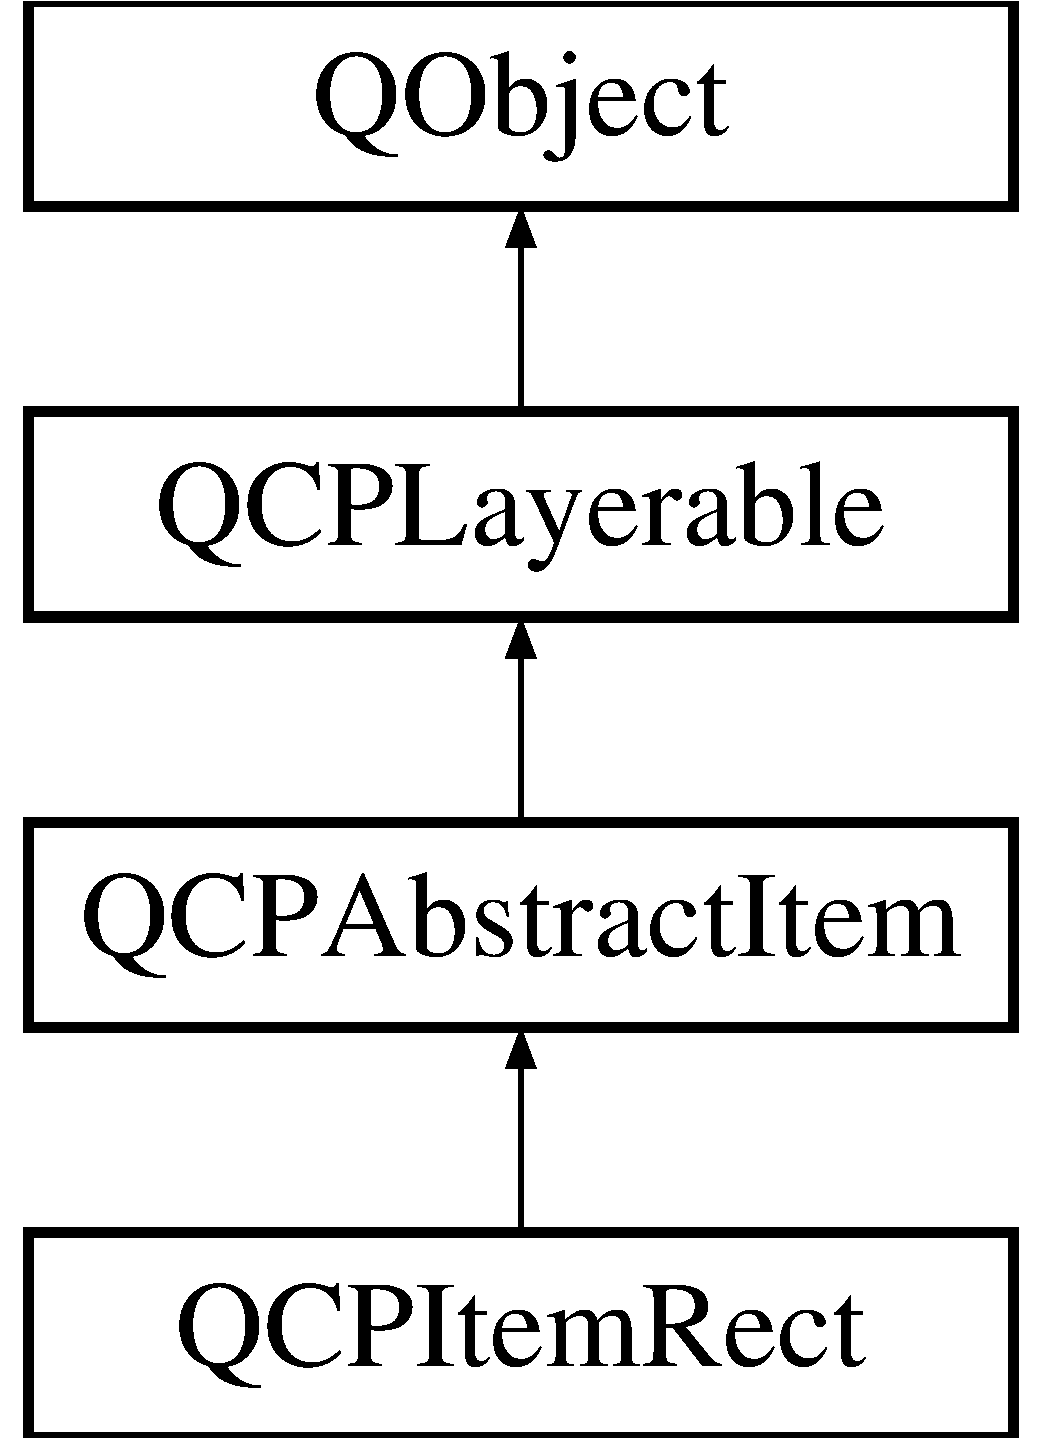
\includegraphics[height=4.000000cm]{class_q_c_p_item_rect}
\end{center}
\end{figure}
\subsection*{Public Member Functions}
\begin{DoxyCompactItemize}
\item 
\hyperlink{class_q_c_p_item_rect_a412ad1579f7a1fba453d0fa28c496cbc}{Q\+C\+P\+Item\+Rect} (\hyperlink{class_q_custom_plot}{Q\+Custom\+Plot} $\ast$parent\+Plot)
\item 
\hypertarget{class_q_c_p_item_rect_a3ee2f580a3950dc11247f405ce8b6ecf}{}\label{class_q_c_p_item_rect_a3ee2f580a3950dc11247f405ce8b6ecf} 
Q\+Pen {\bfseries pen} () const
\item 
\hypertarget{class_q_c_p_item_rect_abd93cf93404ce827dfae71d9d9d08b29}{}\label{class_q_c_p_item_rect_abd93cf93404ce827dfae71d9d9d08b29} 
Q\+Pen {\bfseries selected\+Pen} () const
\item 
\hypertarget{class_q_c_p_item_rect_a5071d7fd864428a1398152aca87b54ad}{}\label{class_q_c_p_item_rect_a5071d7fd864428a1398152aca87b54ad} 
Q\+Brush {\bfseries brush} () const
\item 
\hypertarget{class_q_c_p_item_rect_a2b0a6852bc92d716c7e811c90de2c1a9}{}\label{class_q_c_p_item_rect_a2b0a6852bc92d716c7e811c90de2c1a9} 
Q\+Brush {\bfseries selected\+Brush} () const
\item 
void \hyperlink{class_q_c_p_item_rect_a483c0da5a17e1646cd17ddea2c124e7d}{set\+Pen} (const Q\+Pen \&pen)
\item 
void \hyperlink{class_q_c_p_item_rect_a52a1bcb2dc753a538e406a2ba3cf21ce}{set\+Selected\+Pen} (const Q\+Pen \&pen)
\item 
void \hyperlink{class_q_c_p_item_rect_abbd4e346a03513ee466afc25d9c75446}{set\+Brush} (const Q\+Brush \&brush)
\item 
void \hyperlink{class_q_c_p_item_rect_abd1792859844118dedee86223cede7af}{set\+Selected\+Brush} (const Q\+Brush \&brush)
\item 
virtual double \hyperlink{class_q_c_p_item_rect_abe1a6091591d3bad5e4efab2331f99ec}{select\+Test} (const Q\+PointF \&pos, bool only\+Selectable, Q\+Variant $\ast$details=0) const
\end{DoxyCompactItemize}
\subsection*{Public Attributes}
\begin{DoxyCompactItemize}
\item 
\hypertarget{class_q_c_p_item_rect_aa70feeef173489b03c3fbe906a5023c4}{}\label{class_q_c_p_item_rect_aa70feeef173489b03c3fbe906a5023c4} 
\hyperlink{class_q_c_p_item_position}{Q\+C\+P\+Item\+Position} $\ast$const {\bfseries top\+Left}
\item 
\hypertarget{class_q_c_p_item_rect_a409f3bfe615a7e322bb3d4d193d85b26}{}\label{class_q_c_p_item_rect_a409f3bfe615a7e322bb3d4d193d85b26} 
\hyperlink{class_q_c_p_item_position}{Q\+C\+P\+Item\+Position} $\ast$const {\bfseries bottom\+Right}
\item 
\hypertarget{class_q_c_p_item_rect_a96e50db552fb297d6fb62614676217bc}{}\label{class_q_c_p_item_rect_a96e50db552fb297d6fb62614676217bc} 
\hyperlink{class_q_c_p_item_anchor}{Q\+C\+P\+Item\+Anchor} $\ast$const {\bfseries top}
\item 
\hypertarget{class_q_c_p_item_rect_a77e0eb6e4aa6efee620d35e2c21bdad7}{}\label{class_q_c_p_item_rect_a77e0eb6e4aa6efee620d35e2c21bdad7} 
\hyperlink{class_q_c_p_item_anchor}{Q\+C\+P\+Item\+Anchor} $\ast$const {\bfseries top\+Right}
\item 
\hypertarget{class_q_c_p_item_rect_a7979c1915f61ad2609a9cc179c2e445e}{}\label{class_q_c_p_item_rect_a7979c1915f61ad2609a9cc179c2e445e} 
\hyperlink{class_q_c_p_item_anchor}{Q\+C\+P\+Item\+Anchor} $\ast$const {\bfseries right}
\item 
\hypertarget{class_q_c_p_item_rect_a99313bf2b338d9f81e19bd38082038aa}{}\label{class_q_c_p_item_rect_a99313bf2b338d9f81e19bd38082038aa} 
\hyperlink{class_q_c_p_item_anchor}{Q\+C\+P\+Item\+Anchor} $\ast$const {\bfseries bottom}
\item 
\hypertarget{class_q_c_p_item_rect_abd8ee63fdf81f0c74bf7ccadee8603da}{}\label{class_q_c_p_item_rect_abd8ee63fdf81f0c74bf7ccadee8603da} 
\hyperlink{class_q_c_p_item_anchor}{Q\+C\+P\+Item\+Anchor} $\ast$const {\bfseries bottom\+Left}
\item 
\hypertarget{class_q_c_p_item_rect_aad0ca1af0c8debfc20d7b47fc942764d}{}\label{class_q_c_p_item_rect_aad0ca1af0c8debfc20d7b47fc942764d} 
\hyperlink{class_q_c_p_item_anchor}{Q\+C\+P\+Item\+Anchor} $\ast$const {\bfseries left}
\end{DoxyCompactItemize}
\subsection*{Protected Types}
\begin{DoxyCompactItemize}
\item 
\hypertarget{class_q_c_p_item_rect_af0ebba58e6bca4851c4db726691ec0d3}{}\label{class_q_c_p_item_rect_af0ebba58e6bca4851c4db726691ec0d3} 
enum {\bfseries Anchor\+Index} \{ \newline
{\bfseries ai\+Top}, 
{\bfseries ai\+Top\+Right}, 
{\bfseries ai\+Right}, 
{\bfseries ai\+Bottom}, 
\newline
{\bfseries ai\+Bottom\+Left}, 
{\bfseries ai\+Left}
 \}
\end{DoxyCompactItemize}
\subsection*{Protected Member Functions}
\begin{DoxyCompactItemize}
\item 
\hypertarget{class_q_c_p_item_rect_a18cd583638b876cdd50f1a155ec182aa}{}\label{class_q_c_p_item_rect_a18cd583638b876cdd50f1a155ec182aa} 
virtual void {\bfseries draw} (\hyperlink{class_q_c_p_painter}{Q\+C\+P\+Painter} $\ast$painter)
\item 
\hypertarget{class_q_c_p_item_rect_af1c42e6142d1137673335982856d0ea6}{}\label{class_q_c_p_item_rect_af1c42e6142d1137673335982856d0ea6} 
virtual Q\+PointF {\bfseries anchor\+Pixel\+Point} (int anchor\+Id) const
\item 
\hypertarget{class_q_c_p_item_rect_af94d87da501e9429c0e874f1c0369b03}{}\label{class_q_c_p_item_rect_af94d87da501e9429c0e874f1c0369b03} 
Q\+Pen {\bfseries main\+Pen} () const
\item 
\hypertarget{class_q_c_p_item_rect_a8813d2d670835ac9b8000c981b8ea6fe}{}\label{class_q_c_p_item_rect_a8813d2d670835ac9b8000c981b8ea6fe} 
Q\+Brush {\bfseries main\+Brush} () const
\end{DoxyCompactItemize}
\subsection*{Protected Attributes}
\begin{DoxyCompactItemize}
\item 
\hypertarget{class_q_c_p_item_rect_aa0d49323628d6752026056bfb52afd86}{}\label{class_q_c_p_item_rect_aa0d49323628d6752026056bfb52afd86} 
Q\+Pen {\bfseries m\+Pen}
\item 
\hypertarget{class_q_c_p_item_rect_a73cc0bee61de3c67221ec8c7a76a29ed}{}\label{class_q_c_p_item_rect_a73cc0bee61de3c67221ec8c7a76a29ed} 
Q\+Pen {\bfseries m\+Selected\+Pen}
\item 
\hypertarget{class_q_c_p_item_rect_a2d7f207fada27588b3a52b19234d3c2e}{}\label{class_q_c_p_item_rect_a2d7f207fada27588b3a52b19234d3c2e} 
Q\+Brush {\bfseries m\+Brush}
\item 
\hypertarget{class_q_c_p_item_rect_a21b70eee59b6e19ae0bbdf037b13508f}{}\label{class_q_c_p_item_rect_a21b70eee59b6e19ae0bbdf037b13508f} 
Q\+Brush {\bfseries m\+Selected\+Brush}
\end{DoxyCompactItemize}
\subsection*{Additional Inherited Members}


\subsection{Detailed Description}
A rectangle. 

 It has two positions, {\itshape top\+Left} and {\itshape bottom\+Right}, which define the rectangle. 

\subsection{Constructor \& Destructor Documentation}
\hypertarget{class_q_c_p_item_rect_a412ad1579f7a1fba453d0fa28c496cbc}{}\label{class_q_c_p_item_rect_a412ad1579f7a1fba453d0fa28c496cbc} 
\index{Q\+C\+P\+Item\+Rect@{Q\+C\+P\+Item\+Rect}!Q\+C\+P\+Item\+Rect@{Q\+C\+P\+Item\+Rect}}
\index{Q\+C\+P\+Item\+Rect@{Q\+C\+P\+Item\+Rect}!Q\+C\+P\+Item\+Rect@{Q\+C\+P\+Item\+Rect}}
\subsubsection{\texorpdfstring{Q\+C\+P\+Item\+Rect()}{QCPItemRect()}}
{\footnotesize\ttfamily Q\+C\+P\+Item\+Rect\+::\+Q\+C\+P\+Item\+Rect (\begin{DoxyParamCaption}\item[{\hyperlink{class_q_custom_plot}{Q\+Custom\+Plot} $\ast$}]{parent\+Plot }\end{DoxyParamCaption})}

Creates a rectangle item and sets default values.

The constructed item can be added to the plot with \hyperlink{class_q_custom_plot_aa500620379262321685cb7a7674cbd2a}{Q\+Custom\+Plot\+::add\+Item}. 

\subsection{Member Function Documentation}
\hypertarget{class_q_c_p_item_rect_abe1a6091591d3bad5e4efab2331f99ec}{}\label{class_q_c_p_item_rect_abe1a6091591d3bad5e4efab2331f99ec} 
\index{Q\+C\+P\+Item\+Rect@{Q\+C\+P\+Item\+Rect}!select\+Test@{select\+Test}}
\index{select\+Test@{select\+Test}!Q\+C\+P\+Item\+Rect@{Q\+C\+P\+Item\+Rect}}
\subsubsection{\texorpdfstring{select\+Test()}{selectTest()}}
{\footnotesize\ttfamily double Q\+C\+P\+Item\+Rect\+::select\+Test (\begin{DoxyParamCaption}\item[{const Q\+PointF \&}]{pos,  }\item[{bool}]{only\+Selectable,  }\item[{Q\+Variant $\ast$}]{details = {\ttfamily 0} }\end{DoxyParamCaption}) const\hspace{0.3cm}{\ttfamily [virtual]}}

This function is used to decide whether a click hits a layerable object or not.

{\itshape pos} is a point in pixel coordinates on the \hyperlink{class_q_custom_plot}{Q\+Custom\+Plot} surface. This function returns the shortest pixel distance of this point to the object. If the object is either invisible or the distance couldn\textquotesingle{}t be determined, -\/1.\+0 is returned. Further, if {\itshape only\+Selectable} is true and the object is not selectable, -\/1.\+0 is returned, too.

If the object is represented not by single lines but by an area like a \hyperlink{class_q_c_p_item_text}{Q\+C\+P\+Item\+Text} or the bars of a \hyperlink{class_q_c_p_bars}{Q\+C\+P\+Bars} plottable, a click inside the area should also be considered a hit. In these cases this function thus returns a constant value greater zero but still below the parent plot\textquotesingle{}s selection tolerance. (typically the selection\+Tolerance multiplied by 0.\+99).

Providing a constant value for area objects allows selecting line objects even when they are obscured by such area objects, by clicking close to the lines (i.\+e. closer than 0.\+99$\ast$selection\+Tolerance).

The actual setting of the selection state is not done by this function. This is handled by the parent \hyperlink{class_q_custom_plot}{Q\+Custom\+Plot} when the mouse\+Release\+Event occurs, and the finally selected object is notified via the select\+Event/deselect\+Event methods.

{\itshape details} is an optional output parameter. Every layerable subclass may place any information in {\itshape details}. This information will be passed to select\+Event when the parent \hyperlink{class_q_custom_plot}{Q\+Custom\+Plot} decides on the basis of this select\+Test call, that the object was successfully selected. The subsequent call to select\+Event will carry the {\itshape details}. This is useful for multi-\/part objects (like \hyperlink{class_q_c_p_axis}{Q\+C\+P\+Axis}). This way, a possibly complex calculation to decide which part was clicked is only done once in \hyperlink{class_q_c_p_item_rect_abe1a6091591d3bad5e4efab2331f99ec}{select\+Test}. The result (i.\+e. the actually clicked part) can then be placed in {\itshape details}. So in the subsequent select\+Event, the decision which part was selected doesn\textquotesingle{}t have to be done a second time for a single selection operation.

You may pass 0 as {\itshape details} to indicate that you are not interested in those selection details.

\begin{DoxySeeAlso}{See also}
select\+Event, deselect\+Event, \hyperlink{class_q_custom_plot_a5ee1e2f6ae27419deca53e75907c27e5}{Q\+Custom\+Plot\+::set\+Interactions} 
\end{DoxySeeAlso}


Implements \hyperlink{class_q_c_p_abstract_item_a96d522d10ffc0413b9a366c6f7f0476b}{Q\+C\+P\+Abstract\+Item}.

\hypertarget{class_q_c_p_item_rect_abbd4e346a03513ee466afc25d9c75446}{}\label{class_q_c_p_item_rect_abbd4e346a03513ee466afc25d9c75446} 
\index{Q\+C\+P\+Item\+Rect@{Q\+C\+P\+Item\+Rect}!set\+Brush@{set\+Brush}}
\index{set\+Brush@{set\+Brush}!Q\+C\+P\+Item\+Rect@{Q\+C\+P\+Item\+Rect}}
\subsubsection{\texorpdfstring{set\+Brush()}{setBrush()}}
{\footnotesize\ttfamily void Q\+C\+P\+Item\+Rect\+::set\+Brush (\begin{DoxyParamCaption}\item[{const Q\+Brush \&}]{brush }\end{DoxyParamCaption})}

Sets the brush that will be used to fill the rectangle. To disable filling, set {\itshape brush} to Qt\+::\+No\+Brush.

\begin{DoxySeeAlso}{See also}
\hyperlink{class_q_c_p_item_rect_abd1792859844118dedee86223cede7af}{set\+Selected\+Brush}, \hyperlink{class_q_c_p_item_rect_a483c0da5a17e1646cd17ddea2c124e7d}{set\+Pen} 
\end{DoxySeeAlso}
\hypertarget{class_q_c_p_item_rect_a483c0da5a17e1646cd17ddea2c124e7d}{}\label{class_q_c_p_item_rect_a483c0da5a17e1646cd17ddea2c124e7d} 
\index{Q\+C\+P\+Item\+Rect@{Q\+C\+P\+Item\+Rect}!set\+Pen@{set\+Pen}}
\index{set\+Pen@{set\+Pen}!Q\+C\+P\+Item\+Rect@{Q\+C\+P\+Item\+Rect}}
\subsubsection{\texorpdfstring{set\+Pen()}{setPen()}}
{\footnotesize\ttfamily void Q\+C\+P\+Item\+Rect\+::set\+Pen (\begin{DoxyParamCaption}\item[{const Q\+Pen \&}]{pen }\end{DoxyParamCaption})}

Sets the pen that will be used to draw the line of the rectangle

\begin{DoxySeeAlso}{See also}
\hyperlink{class_q_c_p_item_rect_a52a1bcb2dc753a538e406a2ba3cf21ce}{set\+Selected\+Pen}, \hyperlink{class_q_c_p_item_rect_abbd4e346a03513ee466afc25d9c75446}{set\+Brush} 
\end{DoxySeeAlso}
\hypertarget{class_q_c_p_item_rect_abd1792859844118dedee86223cede7af}{}\label{class_q_c_p_item_rect_abd1792859844118dedee86223cede7af} 
\index{Q\+C\+P\+Item\+Rect@{Q\+C\+P\+Item\+Rect}!set\+Selected\+Brush@{set\+Selected\+Brush}}
\index{set\+Selected\+Brush@{set\+Selected\+Brush}!Q\+C\+P\+Item\+Rect@{Q\+C\+P\+Item\+Rect}}
\subsubsection{\texorpdfstring{set\+Selected\+Brush()}{setSelectedBrush()}}
{\footnotesize\ttfamily void Q\+C\+P\+Item\+Rect\+::set\+Selected\+Brush (\begin{DoxyParamCaption}\item[{const Q\+Brush \&}]{brush }\end{DoxyParamCaption})}

Sets the brush that will be used to fill the rectangle when selected. To disable filling, set {\itshape brush} to Qt\+::\+No\+Brush.

\begin{DoxySeeAlso}{See also}
\hyperlink{class_q_c_p_item_rect_abbd4e346a03513ee466afc25d9c75446}{set\+Brush} 
\end{DoxySeeAlso}
\hypertarget{class_q_c_p_item_rect_a52a1bcb2dc753a538e406a2ba3cf21ce}{}\label{class_q_c_p_item_rect_a52a1bcb2dc753a538e406a2ba3cf21ce} 
\index{Q\+C\+P\+Item\+Rect@{Q\+C\+P\+Item\+Rect}!set\+Selected\+Pen@{set\+Selected\+Pen}}
\index{set\+Selected\+Pen@{set\+Selected\+Pen}!Q\+C\+P\+Item\+Rect@{Q\+C\+P\+Item\+Rect}}
\subsubsection{\texorpdfstring{set\+Selected\+Pen()}{setSelectedPen()}}
{\footnotesize\ttfamily void Q\+C\+P\+Item\+Rect\+::set\+Selected\+Pen (\begin{DoxyParamCaption}\item[{const Q\+Pen \&}]{pen }\end{DoxyParamCaption})}

Sets the pen that will be used to draw the line of the rectangle when selected

\begin{DoxySeeAlso}{See also}
\hyperlink{class_q_c_p_item_rect_a483c0da5a17e1646cd17ddea2c124e7d}{set\+Pen}, \hyperlink{class_q_c_p_abstract_item_a203de94ad586cc44d16c9565f49d3378}{set\+Selected} 
\end{DoxySeeAlso}


The documentation for this class was generated from the following files\+:\begin{DoxyCompactItemize}
\item 
F\+E\+S\+S-\/\+G\+U\+I/\hyperlink{qcustomplot_8h}{qcustomplot.\+h}\item 
F\+E\+S\+S-\/\+G\+U\+I/\hyperlink{qcustomplot_8cpp}{qcustomplot.\+cpp}\end{DoxyCompactItemize}

\hypertarget{class_q_c_p_item_straight_line}{}\section{Q\+C\+P\+Item\+Straight\+Line Class Reference}
\label{class_q_c_p_item_straight_line}\index{Q\+C\+P\+Item\+Straight\+Line@{Q\+C\+P\+Item\+Straight\+Line}}


A straight line that spans infinitely in both directions.  


Inheritance diagram for Q\+C\+P\+Item\+Straight\+Line\+:\begin{figure}[H]
\begin{center}
\leavevmode
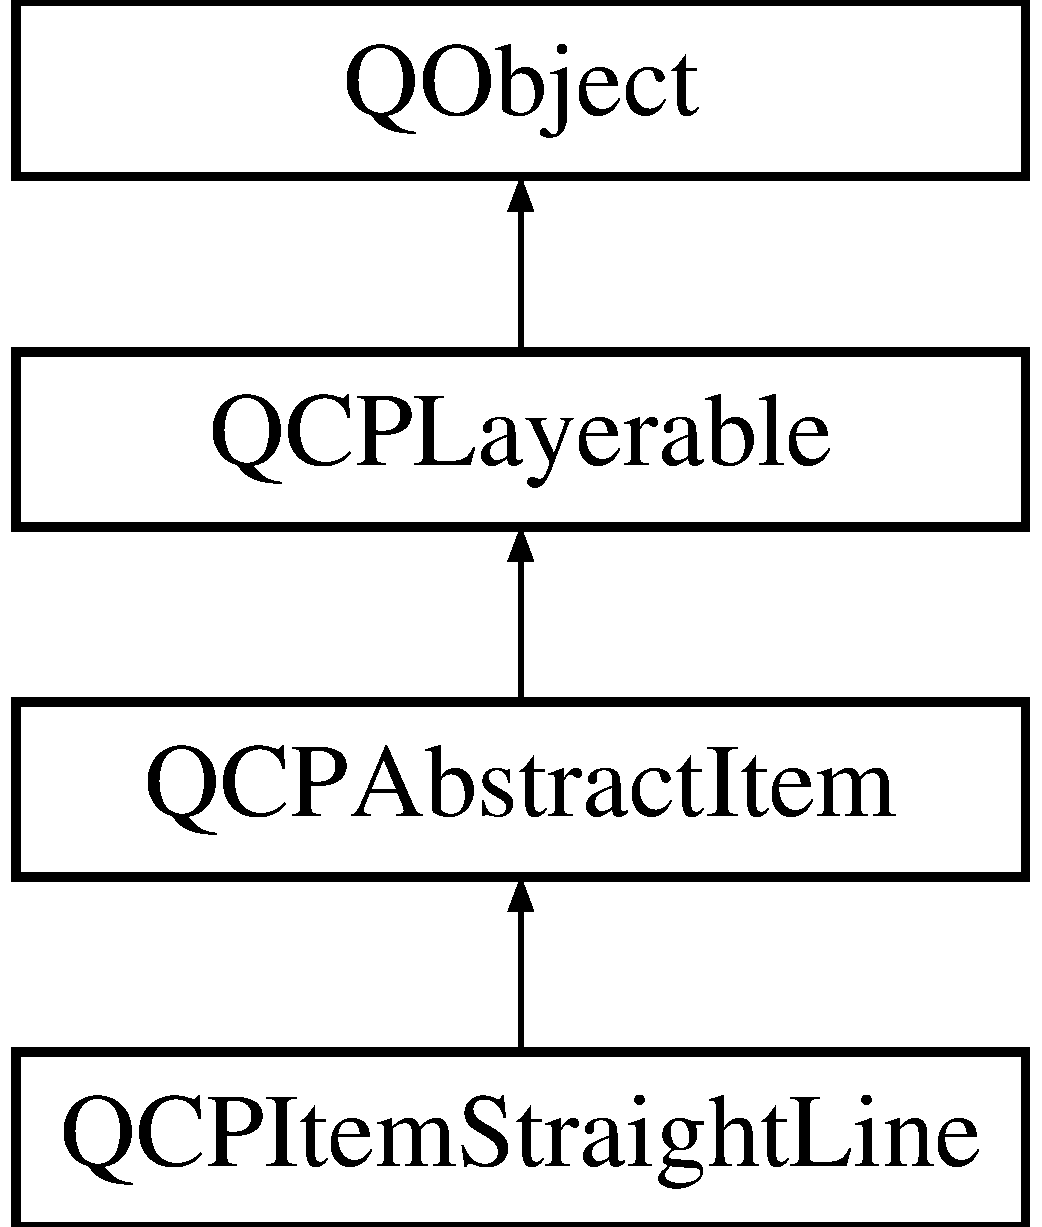
\includegraphics[height=4.000000cm]{class_q_c_p_item_straight_line}
\end{center}
\end{figure}
\subsection*{Public Member Functions}
\begin{DoxyCompactItemize}
\item 
\hyperlink{class_q_c_p_item_straight_line_a41fd2e1f006983449eca9830930c3b10}{Q\+C\+P\+Item\+Straight\+Line} (\hyperlink{class_q_custom_plot}{Q\+Custom\+Plot} $\ast$parent\+Plot)
\item 
\hypertarget{class_q_c_p_item_straight_line_aa751d46cf36073607c11508763f85ff6}{}\label{class_q_c_p_item_straight_line_aa751d46cf36073607c11508763f85ff6} 
Q\+Pen {\bfseries pen} () const
\item 
\hypertarget{class_q_c_p_item_straight_line_ae4a4607045b1d0594f89eee448a31ff9}{}\label{class_q_c_p_item_straight_line_ae4a4607045b1d0594f89eee448a31ff9} 
Q\+Pen {\bfseries selected\+Pen} () const
\item 
void \hyperlink{class_q_c_p_item_straight_line_a9f36c9c9e60d7d9ac084c80380ac8601}{set\+Pen} (const Q\+Pen \&pen)
\item 
void \hyperlink{class_q_c_p_item_straight_line_a5c33559498d33543fa95cf0a36e851ff}{set\+Selected\+Pen} (const Q\+Pen \&pen)
\item 
virtual double \hyperlink{class_q_c_p_item_straight_line_a1e5d99d79efb5871600c72bcd2891a0f}{select\+Test} (const Q\+PointF \&pos, bool only\+Selectable, Q\+Variant $\ast$details=0) const
\end{DoxyCompactItemize}
\subsection*{Public Attributes}
\begin{DoxyCompactItemize}
\item 
\hypertarget{class_q_c_p_item_straight_line_ac131a6ffe456f2cc7364dce541fe0120}{}\label{class_q_c_p_item_straight_line_ac131a6ffe456f2cc7364dce541fe0120} 
\hyperlink{class_q_c_p_item_position}{Q\+C\+P\+Item\+Position} $\ast$const {\bfseries point1}
\item 
\hypertarget{class_q_c_p_item_straight_line_ad26c0a732e471f63f75d481dcd48cfc9}{}\label{class_q_c_p_item_straight_line_ad26c0a732e471f63f75d481dcd48cfc9} 
\hyperlink{class_q_c_p_item_position}{Q\+C\+P\+Item\+Position} $\ast$const {\bfseries point2}
\end{DoxyCompactItemize}
\subsection*{Protected Member Functions}
\begin{DoxyCompactItemize}
\item 
\hypertarget{class_q_c_p_item_straight_line_a2daa1e1253216c26565d56a2d5530170}{}\label{class_q_c_p_item_straight_line_a2daa1e1253216c26565d56a2d5530170} 
virtual void {\bfseries draw} (\hyperlink{class_q_c_p_painter}{Q\+C\+P\+Painter} $\ast$painter)
\item 
\hypertarget{class_q_c_p_item_straight_line_a17107170ed03722e6d626a3ff5a8491c}{}\label{class_q_c_p_item_straight_line_a17107170ed03722e6d626a3ff5a8491c} 
double {\bfseries dist\+To\+Straight\+Line} (const Q\+Vector2D \&point1, const Q\+Vector2D \&vec, const Q\+Vector2D \&point) const
\item 
\hypertarget{class_q_c_p_item_straight_line_af0c893b7196ba210555a8f4332707eab}{}\label{class_q_c_p_item_straight_line_af0c893b7196ba210555a8f4332707eab} 
Q\+LineF {\bfseries get\+Rect\+Clipped\+Straight\+Line} (const Q\+Vector2D \&point1, const Q\+Vector2D \&vec, const Q\+Rect \&rect) const
\item 
\hypertarget{class_q_c_p_item_straight_line_a5b1a39cfc54c3e22f65de2958d40eb59}{}\label{class_q_c_p_item_straight_line_a5b1a39cfc54c3e22f65de2958d40eb59} 
Q\+Pen {\bfseries main\+Pen} () const
\end{DoxyCompactItemize}
\subsection*{Protected Attributes}
\begin{DoxyCompactItemize}
\item 
\hypertarget{class_q_c_p_item_straight_line_a15106ddc2ebd73ed5c1bc57aa92bee8f}{}\label{class_q_c_p_item_straight_line_a15106ddc2ebd73ed5c1bc57aa92bee8f} 
Q\+Pen {\bfseries m\+Pen}
\item 
\hypertarget{class_q_c_p_item_straight_line_a0307a0d56a018656adbf798bc84c2a4b}{}\label{class_q_c_p_item_straight_line_a0307a0d56a018656adbf798bc84c2a4b} 
Q\+Pen {\bfseries m\+Selected\+Pen}
\end{DoxyCompactItemize}
\subsection*{Additional Inherited Members}


\subsection{Detailed Description}
A straight line that spans infinitely in both directions. 

 It has two positions, {\itshape point1} and {\itshape point2}, which define the straight line. 

\subsection{Constructor \& Destructor Documentation}
\hypertarget{class_q_c_p_item_straight_line_a41fd2e1f006983449eca9830930c3b10}{}\label{class_q_c_p_item_straight_line_a41fd2e1f006983449eca9830930c3b10} 
\index{Q\+C\+P\+Item\+Straight\+Line@{Q\+C\+P\+Item\+Straight\+Line}!Q\+C\+P\+Item\+Straight\+Line@{Q\+C\+P\+Item\+Straight\+Line}}
\index{Q\+C\+P\+Item\+Straight\+Line@{Q\+C\+P\+Item\+Straight\+Line}!Q\+C\+P\+Item\+Straight\+Line@{Q\+C\+P\+Item\+Straight\+Line}}
\subsubsection{\texorpdfstring{Q\+C\+P\+Item\+Straight\+Line()}{QCPItemStraightLine()}}
{\footnotesize\ttfamily Q\+C\+P\+Item\+Straight\+Line\+::\+Q\+C\+P\+Item\+Straight\+Line (\begin{DoxyParamCaption}\item[{\hyperlink{class_q_custom_plot}{Q\+Custom\+Plot} $\ast$}]{parent\+Plot }\end{DoxyParamCaption})}

Creates a straight line item and sets default values.

The constructed item can be added to the plot with \hyperlink{class_q_custom_plot_aa500620379262321685cb7a7674cbd2a}{Q\+Custom\+Plot\+::add\+Item}. 

\subsection{Member Function Documentation}
\hypertarget{class_q_c_p_item_straight_line_a1e5d99d79efb5871600c72bcd2891a0f}{}\label{class_q_c_p_item_straight_line_a1e5d99d79efb5871600c72bcd2891a0f} 
\index{Q\+C\+P\+Item\+Straight\+Line@{Q\+C\+P\+Item\+Straight\+Line}!select\+Test@{select\+Test}}
\index{select\+Test@{select\+Test}!Q\+C\+P\+Item\+Straight\+Line@{Q\+C\+P\+Item\+Straight\+Line}}
\subsubsection{\texorpdfstring{select\+Test()}{selectTest()}}
{\footnotesize\ttfamily double Q\+C\+P\+Item\+Straight\+Line\+::select\+Test (\begin{DoxyParamCaption}\item[{const Q\+PointF \&}]{pos,  }\item[{bool}]{only\+Selectable,  }\item[{Q\+Variant $\ast$}]{details = {\ttfamily 0} }\end{DoxyParamCaption}) const\hspace{0.3cm}{\ttfamily [virtual]}}

This function is used to decide whether a click hits a layerable object or not.

{\itshape pos} is a point in pixel coordinates on the \hyperlink{class_q_custom_plot}{Q\+Custom\+Plot} surface. This function returns the shortest pixel distance of this point to the object. If the object is either invisible or the distance couldn\textquotesingle{}t be determined, -\/1.\+0 is returned. Further, if {\itshape only\+Selectable} is true and the object is not selectable, -\/1.\+0 is returned, too.

If the object is represented not by single lines but by an area like a \hyperlink{class_q_c_p_item_text}{Q\+C\+P\+Item\+Text} or the bars of a \hyperlink{class_q_c_p_bars}{Q\+C\+P\+Bars} plottable, a click inside the area should also be considered a hit. In these cases this function thus returns a constant value greater zero but still below the parent plot\textquotesingle{}s selection tolerance. (typically the selection\+Tolerance multiplied by 0.\+99).

Providing a constant value for area objects allows selecting line objects even when they are obscured by such area objects, by clicking close to the lines (i.\+e. closer than 0.\+99$\ast$selection\+Tolerance).

The actual setting of the selection state is not done by this function. This is handled by the parent \hyperlink{class_q_custom_plot}{Q\+Custom\+Plot} when the mouse\+Release\+Event occurs, and the finally selected object is notified via the select\+Event/deselect\+Event methods.

{\itshape details} is an optional output parameter. Every layerable subclass may place any information in {\itshape details}. This information will be passed to select\+Event when the parent \hyperlink{class_q_custom_plot}{Q\+Custom\+Plot} decides on the basis of this select\+Test call, that the object was successfully selected. The subsequent call to select\+Event will carry the {\itshape details}. This is useful for multi-\/part objects (like \hyperlink{class_q_c_p_axis}{Q\+C\+P\+Axis}). This way, a possibly complex calculation to decide which part was clicked is only done once in \hyperlink{class_q_c_p_item_straight_line_a1e5d99d79efb5871600c72bcd2891a0f}{select\+Test}. The result (i.\+e. the actually clicked part) can then be placed in {\itshape details}. So in the subsequent select\+Event, the decision which part was selected doesn\textquotesingle{}t have to be done a second time for a single selection operation.

You may pass 0 as {\itshape details} to indicate that you are not interested in those selection details.

\begin{DoxySeeAlso}{See also}
select\+Event, deselect\+Event, \hyperlink{class_q_custom_plot_a5ee1e2f6ae27419deca53e75907c27e5}{Q\+Custom\+Plot\+::set\+Interactions} 
\end{DoxySeeAlso}


Implements \hyperlink{class_q_c_p_abstract_item_a96d522d10ffc0413b9a366c6f7f0476b}{Q\+C\+P\+Abstract\+Item}.

\hypertarget{class_q_c_p_item_straight_line_a9f36c9c9e60d7d9ac084c80380ac8601}{}\label{class_q_c_p_item_straight_line_a9f36c9c9e60d7d9ac084c80380ac8601} 
\index{Q\+C\+P\+Item\+Straight\+Line@{Q\+C\+P\+Item\+Straight\+Line}!set\+Pen@{set\+Pen}}
\index{set\+Pen@{set\+Pen}!Q\+C\+P\+Item\+Straight\+Line@{Q\+C\+P\+Item\+Straight\+Line}}
\subsubsection{\texorpdfstring{set\+Pen()}{setPen()}}
{\footnotesize\ttfamily void Q\+C\+P\+Item\+Straight\+Line\+::set\+Pen (\begin{DoxyParamCaption}\item[{const Q\+Pen \&}]{pen }\end{DoxyParamCaption})}

Sets the pen that will be used to draw the line

\begin{DoxySeeAlso}{See also}
\hyperlink{class_q_c_p_item_straight_line_a5c33559498d33543fa95cf0a36e851ff}{set\+Selected\+Pen} 
\end{DoxySeeAlso}
\hypertarget{class_q_c_p_item_straight_line_a5c33559498d33543fa95cf0a36e851ff}{}\label{class_q_c_p_item_straight_line_a5c33559498d33543fa95cf0a36e851ff} 
\index{Q\+C\+P\+Item\+Straight\+Line@{Q\+C\+P\+Item\+Straight\+Line}!set\+Selected\+Pen@{set\+Selected\+Pen}}
\index{set\+Selected\+Pen@{set\+Selected\+Pen}!Q\+C\+P\+Item\+Straight\+Line@{Q\+C\+P\+Item\+Straight\+Line}}
\subsubsection{\texorpdfstring{set\+Selected\+Pen()}{setSelectedPen()}}
{\footnotesize\ttfamily void Q\+C\+P\+Item\+Straight\+Line\+::set\+Selected\+Pen (\begin{DoxyParamCaption}\item[{const Q\+Pen \&}]{pen }\end{DoxyParamCaption})}

Sets the pen that will be used to draw the line when selected

\begin{DoxySeeAlso}{See also}
\hyperlink{class_q_c_p_item_straight_line_a9f36c9c9e60d7d9ac084c80380ac8601}{set\+Pen}, \hyperlink{class_q_c_p_abstract_item_a203de94ad586cc44d16c9565f49d3378}{set\+Selected} 
\end{DoxySeeAlso}


The documentation for this class was generated from the following files\+:\begin{DoxyCompactItemize}
\item 
C\+:/\+Users/\+Jesse Jutson/\+Documents/\+Git\+Hub/\+F\+E\+S\+S\+G\+U\+I/\+F\+E\+S\+S-\/\+G\+U\+I/\hyperlink{qcustomplot_8h}{qcustomplot.\+h}\item 
C\+:/\+Users/\+Jesse Jutson/\+Documents/\+Git\+Hub/\+F\+E\+S\+S\+G\+U\+I/\+F\+E\+S\+S-\/\+G\+U\+I/\hyperlink{qcustomplot_8cpp}{qcustomplot.\+cpp}\end{DoxyCompactItemize}

\hypertarget{class_q_c_p_item_text}{}\section{Q\+C\+P\+Item\+Text Class Reference}
\label{class_q_c_p_item_text}\index{Q\+C\+P\+Item\+Text@{Q\+C\+P\+Item\+Text}}


A text label.  


Inheritance diagram for Q\+C\+P\+Item\+Text\+:\begin{figure}[H]
\begin{center}
\leavevmode
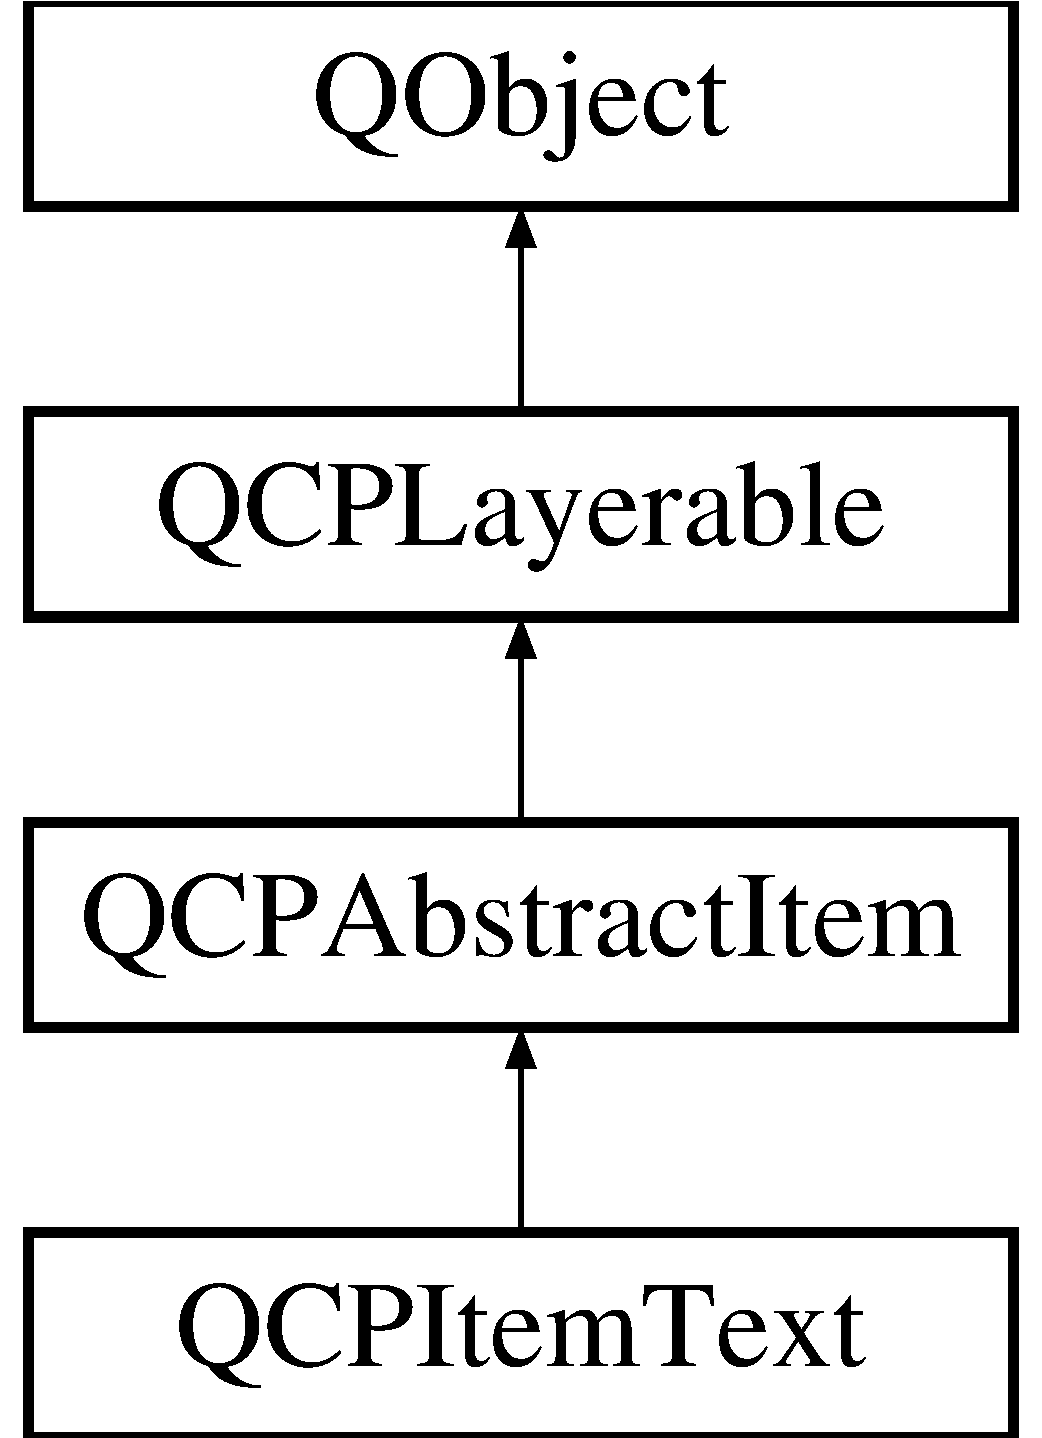
\includegraphics[height=4.000000cm]{class_q_c_p_item_text}
\end{center}
\end{figure}
\subsection*{Public Member Functions}
\begin{DoxyCompactItemize}
\item 
\hyperlink{class_q_c_p_item_text_a77ff96a2972a00872ff8f8c67143abbe}{Q\+C\+P\+Item\+Text} (\hyperlink{class_q_custom_plot}{Q\+Custom\+Plot} $\ast$parent\+Plot)
\item 
\hypertarget{class_q_c_p_item_text_a071ec7567ae4deae2262a5b861df7d54}{}\label{class_q_c_p_item_text_a071ec7567ae4deae2262a5b861df7d54} 
Q\+Color {\bfseries color} () const
\item 
\hypertarget{class_q_c_p_item_text_a6e13d5497ea634fe1ee9f4aac94f664c}{}\label{class_q_c_p_item_text_a6e13d5497ea634fe1ee9f4aac94f664c} 
Q\+Color {\bfseries selected\+Color} () const
\item 
\hypertarget{class_q_c_p_item_text_a7039d313069547682f28688448333979}{}\label{class_q_c_p_item_text_a7039d313069547682f28688448333979} 
Q\+Pen {\bfseries pen} () const
\item 
\hypertarget{class_q_c_p_item_text_a852a79afa0e88e29e11474d323440126}{}\label{class_q_c_p_item_text_a852a79afa0e88e29e11474d323440126} 
Q\+Pen {\bfseries selected\+Pen} () const
\item 
\hypertarget{class_q_c_p_item_text_a2600b9b419f17e2e2381f5ed8267da62}{}\label{class_q_c_p_item_text_a2600b9b419f17e2e2381f5ed8267da62} 
Q\+Brush {\bfseries brush} () const
\item 
\hypertarget{class_q_c_p_item_text_a300770cc32acf3e92763651803482563}{}\label{class_q_c_p_item_text_a300770cc32acf3e92763651803482563} 
Q\+Brush {\bfseries selected\+Brush} () const
\item 
\hypertarget{class_q_c_p_item_text_a44a564431890ffdfe0f978f8732cfb81}{}\label{class_q_c_p_item_text_a44a564431890ffdfe0f978f8732cfb81} 
Q\+Font {\bfseries font} () const
\item 
\hypertarget{class_q_c_p_item_text_a74c947c6193e3b47884fac84fdb29922}{}\label{class_q_c_p_item_text_a74c947c6193e3b47884fac84fdb29922} 
Q\+Font {\bfseries selected\+Font} () const
\item 
\hypertarget{class_q_c_p_item_text_ad71c9e83ee3556d9d617eca854e8eb18}{}\label{class_q_c_p_item_text_ad71c9e83ee3556d9d617eca854e8eb18} 
Q\+String {\bfseries text} () const
\item 
\hypertarget{class_q_c_p_item_text_a0d946dca3008d353afd04b4337739199}{}\label{class_q_c_p_item_text_a0d946dca3008d353afd04b4337739199} 
Qt\+::\+Alignment {\bfseries position\+Alignment} () const
\item 
\hypertarget{class_q_c_p_item_text_a9af3198d46551e1cc7703f02c95ddfe5}{}\label{class_q_c_p_item_text_a9af3198d46551e1cc7703f02c95ddfe5} 
Qt\+::\+Alignment {\bfseries text\+Alignment} () const
\item 
\hypertarget{class_q_c_p_item_text_a035962b4ed23ff0a89e6a8b46fa18bf1}{}\label{class_q_c_p_item_text_a035962b4ed23ff0a89e6a8b46fa18bf1} 
double {\bfseries rotation} () const
\item 
\hypertarget{class_q_c_p_item_text_a5a598618350b40446d031fa9dc15fba7}{}\label{class_q_c_p_item_text_a5a598618350b40446d031fa9dc15fba7} 
Q\+Margins {\bfseries padding} () const
\item 
void \hyperlink{class_q_c_p_item_text_aa51efc0841fe52da9eaf8aff6fc8a8b2}{set\+Color} (const Q\+Color \&color)
\item 
void \hyperlink{class_q_c_p_item_text_ae7ba0bdb75c897b028388e45bfd435fa}{set\+Selected\+Color} (const Q\+Color \&color)
\item 
void \hyperlink{class_q_c_p_item_text_a9b9ec6eea0eb0603977ff84d4c78d0a3}{set\+Pen} (const Q\+Pen \&pen)
\item 
void \hyperlink{class_q_c_p_item_text_a291febe586f0da3f1c392e77bef4aa20}{set\+Selected\+Pen} (const Q\+Pen \&pen)
\item 
void \hyperlink{class_q_c_p_item_text_a1c7e131516df2ed8d941ef31240ded8e}{set\+Brush} (const Q\+Brush \&brush)
\item 
void \hyperlink{class_q_c_p_item_text_a6b8377eeb2af75eb9528422671ac16cb}{set\+Selected\+Brush} (const Q\+Brush \&brush)
\item 
void \hyperlink{class_q_c_p_item_text_a94ad60ebe04f5c07c35e7c2029e96b1f}{set\+Font} (const Q\+Font \&font)
\item 
void \hyperlink{class_q_c_p_item_text_a0be2841772f83663c4db307928b82816}{set\+Selected\+Font} (const Q\+Font \&font)
\item 
void \hyperlink{class_q_c_p_item_text_a3dacdda0ac88f99a05b333b977c48747}{set\+Text} (const Q\+String \&text)
\item 
void \hyperlink{class_q_c_p_item_text_a781cdf8c640fc6a055dcff1e675c8c7a}{set\+Position\+Alignment} (Qt\+::\+Alignment alignment)
\item 
void \hyperlink{class_q_c_p_item_text_ab5bc0684c4d1bed81949a11b34dba478}{set\+Text\+Alignment} (Qt\+::\+Alignment alignment)
\item 
void \hyperlink{class_q_c_p_item_text_a4bcc10cd97952c3f749d75824b5077f0}{set\+Rotation} (double degrees)
\item 
void \hyperlink{class_q_c_p_item_text_aeea8a3e01f135f9dd0bb08f51db66310}{set\+Padding} (const Q\+Margins \&padding)
\item 
virtual double \hyperlink{class_q_c_p_item_text_aca74494fd5e769f331a6eb3e29f32916}{select\+Test} (const Q\+PointF \&pos, bool only\+Selectable, Q\+Variant $\ast$details=0) const
\end{DoxyCompactItemize}
\subsection*{Public Attributes}
\begin{DoxyCompactItemize}
\item 
\hypertarget{class_q_c_p_item_text_a0d228a00e819022b5690c65762721129}{}\label{class_q_c_p_item_text_a0d228a00e819022b5690c65762721129} 
\hyperlink{class_q_c_p_item_position}{Q\+C\+P\+Item\+Position} $\ast$const {\bfseries position}
\item 
\hypertarget{class_q_c_p_item_text_a6354d8762182a3502103fabe5fbb8512}{}\label{class_q_c_p_item_text_a6354d8762182a3502103fabe5fbb8512} 
\hyperlink{class_q_c_p_item_anchor}{Q\+C\+P\+Item\+Anchor} $\ast$const {\bfseries top\+Left}
\item 
\hypertarget{class_q_c_p_item_text_a5c87ee162cbbe3d166b97826c8849304}{}\label{class_q_c_p_item_text_a5c87ee162cbbe3d166b97826c8849304} 
\hyperlink{class_q_c_p_item_anchor}{Q\+C\+P\+Item\+Anchor} $\ast$const {\bfseries top}
\item 
\hypertarget{class_q_c_p_item_text_ad18ac45cb4cc135de1eb78f2e86b6504}{}\label{class_q_c_p_item_text_ad18ac45cb4cc135de1eb78f2e86b6504} 
\hyperlink{class_q_c_p_item_anchor}{Q\+C\+P\+Item\+Anchor} $\ast$const {\bfseries top\+Right}
\item 
\hypertarget{class_q_c_p_item_text_aef159622ce6502412e782a21ba6d84f2}{}\label{class_q_c_p_item_text_aef159622ce6502412e782a21ba6d84f2} 
\hyperlink{class_q_c_p_item_anchor}{Q\+C\+P\+Item\+Anchor} $\ast$const {\bfseries right}
\item 
\hypertarget{class_q_c_p_item_text_a8ad47045c29af43b0312f7d93bb74374}{}\label{class_q_c_p_item_text_a8ad47045c29af43b0312f7d93bb74374} 
\hyperlink{class_q_c_p_item_anchor}{Q\+C\+P\+Item\+Anchor} $\ast$const {\bfseries bottom\+Right}
\item 
\hypertarget{class_q_c_p_item_text_a94aeec080f877d3d1d0c3d8ffc10e9e6}{}\label{class_q_c_p_item_text_a94aeec080f877d3d1d0c3d8ffc10e9e6} 
\hyperlink{class_q_c_p_item_anchor}{Q\+C\+P\+Item\+Anchor} $\ast$const {\bfseries bottom}
\item 
\hypertarget{class_q_c_p_item_text_a6a1c872ad3789ecafcaeac2066e218a0}{}\label{class_q_c_p_item_text_a6a1c872ad3789ecafcaeac2066e218a0} 
\hyperlink{class_q_c_p_item_anchor}{Q\+C\+P\+Item\+Anchor} $\ast$const {\bfseries bottom\+Left}
\item 
\hypertarget{class_q_c_p_item_text_ab8c6c6e1df36256986fab1463c0a1d38}{}\label{class_q_c_p_item_text_ab8c6c6e1df36256986fab1463c0a1d38} 
\hyperlink{class_q_c_p_item_anchor}{Q\+C\+P\+Item\+Anchor} $\ast$const {\bfseries left}
\end{DoxyCompactItemize}
\subsection*{Protected Types}
\begin{DoxyCompactItemize}
\item 
\hypertarget{class_q_c_p_item_text_a14a84e58f72519c8ae1d7a4a1dd23f21}{}\label{class_q_c_p_item_text_a14a84e58f72519c8ae1d7a4a1dd23f21} 
enum {\bfseries Anchor\+Index} \{ \newline
{\bfseries ai\+Top\+Left}, 
{\bfseries ai\+Top}, 
{\bfseries ai\+Top\+Right}, 
{\bfseries ai\+Right}, 
\newline
{\bfseries ai\+Bottom\+Right}, 
{\bfseries ai\+Bottom}, 
{\bfseries ai\+Bottom\+Left}, 
{\bfseries ai\+Left}
 \}
\end{DoxyCompactItemize}
\subsection*{Protected Member Functions}
\begin{DoxyCompactItemize}
\item 
\hypertarget{class_q_c_p_item_text_a8793adb271ab79b4cf391dc55e9987f1}{}\label{class_q_c_p_item_text_a8793adb271ab79b4cf391dc55e9987f1} 
virtual void {\bfseries draw} (\hyperlink{class_q_c_p_painter}{Q\+C\+P\+Painter} $\ast$painter)
\item 
\hypertarget{class_q_c_p_item_text_a3f999a0a7664421373601206bc35cc7c}{}\label{class_q_c_p_item_text_a3f999a0a7664421373601206bc35cc7c} 
virtual Q\+PointF {\bfseries anchor\+Pixel\+Point} (int anchor\+Id) const
\item 
\hypertarget{class_q_c_p_item_text_a4c76ad7e33c50aff0a60b8f38fe6060e}{}\label{class_q_c_p_item_text_a4c76ad7e33c50aff0a60b8f38fe6060e} 
Q\+PointF {\bfseries get\+Text\+Draw\+Point} (const Q\+PointF \&pos, const Q\+RectF \&rect, Qt\+::\+Alignment position\+Alignment) const
\item 
\hypertarget{class_q_c_p_item_text_af30ac2a0b84afa86a1dec22ab48dd07d}{}\label{class_q_c_p_item_text_af30ac2a0b84afa86a1dec22ab48dd07d} 
Q\+Font {\bfseries main\+Font} () const
\item 
\hypertarget{class_q_c_p_item_text_abe3f10805baf62797cb91fd4a4464fcc}{}\label{class_q_c_p_item_text_abe3f10805baf62797cb91fd4a4464fcc} 
Q\+Color {\bfseries main\+Color} () const
\item 
\hypertarget{class_q_c_p_item_text_a2f67fcbb7ac10ea9a94c4ecc3b0f4dfc}{}\label{class_q_c_p_item_text_a2f67fcbb7ac10ea9a94c4ecc3b0f4dfc} 
Q\+Pen {\bfseries main\+Pen} () const
\item 
\hypertarget{class_q_c_p_item_text_acddddd3ce88cfc87ab57b1ec4b25acb9}{}\label{class_q_c_p_item_text_acddddd3ce88cfc87ab57b1ec4b25acb9} 
Q\+Brush {\bfseries main\+Brush} () const
\end{DoxyCompactItemize}
\subsection*{Protected Attributes}
\begin{DoxyCompactItemize}
\item 
\hypertarget{class_q_c_p_item_text_a8407f284ad867f627878cc26ef433d08}{}\label{class_q_c_p_item_text_a8407f284ad867f627878cc26ef433d08} 
Q\+Color {\bfseries m\+Color}
\item 
\hypertarget{class_q_c_p_item_text_a7eb64e42f5f7998a97d8907ad25933c1}{}\label{class_q_c_p_item_text_a7eb64e42f5f7998a97d8907ad25933c1} 
Q\+Color {\bfseries m\+Selected\+Color}
\item 
\hypertarget{class_q_c_p_item_text_aa02388705dbbff1bf7b8aa872b5f579c}{}\label{class_q_c_p_item_text_aa02388705dbbff1bf7b8aa872b5f579c} 
Q\+Pen {\bfseries m\+Pen}
\item 
\hypertarget{class_q_c_p_item_text_a8eaec649606d6ead2d8d4dcb5691777c}{}\label{class_q_c_p_item_text_a8eaec649606d6ead2d8d4dcb5691777c} 
Q\+Pen {\bfseries m\+Selected\+Pen}
\item 
\hypertarget{class_q_c_p_item_text_a2535911875faa459b8337f2efccb5cb8}{}\label{class_q_c_p_item_text_a2535911875faa459b8337f2efccb5cb8} 
Q\+Brush {\bfseries m\+Brush}
\item 
\hypertarget{class_q_c_p_item_text_a28ccd097b42a216d81db9c6869f54a59}{}\label{class_q_c_p_item_text_a28ccd097b42a216d81db9c6869f54a59} 
Q\+Brush {\bfseries m\+Selected\+Brush}
\item 
\hypertarget{class_q_c_p_item_text_a1dc87fe2a824820d549ffd7e644eef8d}{}\label{class_q_c_p_item_text_a1dc87fe2a824820d549ffd7e644eef8d} 
Q\+Font {\bfseries m\+Font}
\item 
\hypertarget{class_q_c_p_item_text_a6702f141fae590b2f4f1ec02fe9f8bd5}{}\label{class_q_c_p_item_text_a6702f141fae590b2f4f1ec02fe9f8bd5} 
Q\+Font {\bfseries m\+Selected\+Font}
\item 
\hypertarget{class_q_c_p_item_text_a2dec3e08c11f51639629374ecec3bd62}{}\label{class_q_c_p_item_text_a2dec3e08c11f51639629374ecec3bd62} 
Q\+String {\bfseries m\+Text}
\item 
\hypertarget{class_q_c_p_item_text_a6c27f7dc1a962a04b32430cf99f04654}{}\label{class_q_c_p_item_text_a6c27f7dc1a962a04b32430cf99f04654} 
Qt\+::\+Alignment {\bfseries m\+Position\+Alignment}
\item 
\hypertarget{class_q_c_p_item_text_acdb2e50c38e83da00f083771efbd213f}{}\label{class_q_c_p_item_text_acdb2e50c38e83da00f083771efbd213f} 
Qt\+::\+Alignment {\bfseries m\+Text\+Alignment}
\item 
\hypertarget{class_q_c_p_item_text_ac37df0061552225d2277e1ee3b48f2cb}{}\label{class_q_c_p_item_text_ac37df0061552225d2277e1ee3b48f2cb} 
double {\bfseries m\+Rotation}
\item 
\hypertarget{class_q_c_p_item_text_ae7b3ef0ce6046efd4b346d28f2e1fb67}{}\label{class_q_c_p_item_text_ae7b3ef0ce6046efd4b346d28f2e1fb67} 
Q\+Margins {\bfseries m\+Padding}
\end{DoxyCompactItemize}
\subsection*{Additional Inherited Members}


\subsection{Detailed Description}
A text label. 

 Its position is defined by the member {\itshape position} and the setting of \hyperlink{class_q_c_p_item_text_a781cdf8c640fc6a055dcff1e675c8c7a}{set\+Position\+Alignment}. The latter controls which part of the text rect shall be aligned with {\itshape position}.

The text alignment itself (i.\+e. left, center, right) can be controlled with \hyperlink{class_q_c_p_item_text_ab5bc0684c4d1bed81949a11b34dba478}{set\+Text\+Alignment}.

The text may be rotated around the {\itshape position} point with \hyperlink{class_q_c_p_item_text_a4bcc10cd97952c3f749d75824b5077f0}{set\+Rotation}. 

\subsection{Constructor \& Destructor Documentation}
\hypertarget{class_q_c_p_item_text_a77ff96a2972a00872ff8f8c67143abbe}{}\label{class_q_c_p_item_text_a77ff96a2972a00872ff8f8c67143abbe} 
\index{Q\+C\+P\+Item\+Text@{Q\+C\+P\+Item\+Text}!Q\+C\+P\+Item\+Text@{Q\+C\+P\+Item\+Text}}
\index{Q\+C\+P\+Item\+Text@{Q\+C\+P\+Item\+Text}!Q\+C\+P\+Item\+Text@{Q\+C\+P\+Item\+Text}}
\subsubsection{\texorpdfstring{Q\+C\+P\+Item\+Text()}{QCPItemText()}}
{\footnotesize\ttfamily Q\+C\+P\+Item\+Text\+::\+Q\+C\+P\+Item\+Text (\begin{DoxyParamCaption}\item[{\hyperlink{class_q_custom_plot}{Q\+Custom\+Plot} $\ast$}]{parent\+Plot }\end{DoxyParamCaption})}

Creates a text item and sets default values.

The constructed item can be added to the plot with \hyperlink{class_q_custom_plot_aa500620379262321685cb7a7674cbd2a}{Q\+Custom\+Plot\+::add\+Item}. 

\subsection{Member Function Documentation}
\hypertarget{class_q_c_p_item_text_aca74494fd5e769f331a6eb3e29f32916}{}\label{class_q_c_p_item_text_aca74494fd5e769f331a6eb3e29f32916} 
\index{Q\+C\+P\+Item\+Text@{Q\+C\+P\+Item\+Text}!select\+Test@{select\+Test}}
\index{select\+Test@{select\+Test}!Q\+C\+P\+Item\+Text@{Q\+C\+P\+Item\+Text}}
\subsubsection{\texorpdfstring{select\+Test()}{selectTest()}}
{\footnotesize\ttfamily double Q\+C\+P\+Item\+Text\+::select\+Test (\begin{DoxyParamCaption}\item[{const Q\+PointF \&}]{pos,  }\item[{bool}]{only\+Selectable,  }\item[{Q\+Variant $\ast$}]{details = {\ttfamily 0} }\end{DoxyParamCaption}) const\hspace{0.3cm}{\ttfamily [virtual]}}

This function is used to decide whether a click hits a layerable object or not.

{\itshape pos} is a point in pixel coordinates on the \hyperlink{class_q_custom_plot}{Q\+Custom\+Plot} surface. This function returns the shortest pixel distance of this point to the object. If the object is either invisible or the distance couldn\textquotesingle{}t be determined, -\/1.\+0 is returned. Further, if {\itshape only\+Selectable} is true and the object is not selectable, -\/1.\+0 is returned, too.

If the object is represented not by single lines but by an area like a \hyperlink{class_q_c_p_item_text}{Q\+C\+P\+Item\+Text} or the bars of a \hyperlink{class_q_c_p_bars}{Q\+C\+P\+Bars} plottable, a click inside the area should also be considered a hit. In these cases this function thus returns a constant value greater zero but still below the parent plot\textquotesingle{}s selection tolerance. (typically the selection\+Tolerance multiplied by 0.\+99).

Providing a constant value for area objects allows selecting line objects even when they are obscured by such area objects, by clicking close to the lines (i.\+e. closer than 0.\+99$\ast$selection\+Tolerance).

The actual setting of the selection state is not done by this function. This is handled by the parent \hyperlink{class_q_custom_plot}{Q\+Custom\+Plot} when the mouse\+Release\+Event occurs, and the finally selected object is notified via the select\+Event/deselect\+Event methods.

{\itshape details} is an optional output parameter. Every layerable subclass may place any information in {\itshape details}. This information will be passed to select\+Event when the parent \hyperlink{class_q_custom_plot}{Q\+Custom\+Plot} decides on the basis of this select\+Test call, that the object was successfully selected. The subsequent call to select\+Event will carry the {\itshape details}. This is useful for multi-\/part objects (like \hyperlink{class_q_c_p_axis}{Q\+C\+P\+Axis}). This way, a possibly complex calculation to decide which part was clicked is only done once in \hyperlink{class_q_c_p_item_text_aca74494fd5e769f331a6eb3e29f32916}{select\+Test}. The result (i.\+e. the actually clicked part) can then be placed in {\itshape details}. So in the subsequent select\+Event, the decision which part was selected doesn\textquotesingle{}t have to be done a second time for a single selection operation.

You may pass 0 as {\itshape details} to indicate that you are not interested in those selection details.

\begin{DoxySeeAlso}{See also}
select\+Event, deselect\+Event, \hyperlink{class_q_custom_plot_a5ee1e2f6ae27419deca53e75907c27e5}{Q\+Custom\+Plot\+::set\+Interactions} 
\end{DoxySeeAlso}


Implements \hyperlink{class_q_c_p_abstract_item_a96d522d10ffc0413b9a366c6f7f0476b}{Q\+C\+P\+Abstract\+Item}.

\hypertarget{class_q_c_p_item_text_a1c7e131516df2ed8d941ef31240ded8e}{}\label{class_q_c_p_item_text_a1c7e131516df2ed8d941ef31240ded8e} 
\index{Q\+C\+P\+Item\+Text@{Q\+C\+P\+Item\+Text}!set\+Brush@{set\+Brush}}
\index{set\+Brush@{set\+Brush}!Q\+C\+P\+Item\+Text@{Q\+C\+P\+Item\+Text}}
\subsubsection{\texorpdfstring{set\+Brush()}{setBrush()}}
{\footnotesize\ttfamily void Q\+C\+P\+Item\+Text\+::set\+Brush (\begin{DoxyParamCaption}\item[{const Q\+Brush \&}]{brush }\end{DoxyParamCaption})}

Sets the brush that will be used do fill the background of the text. To disable the background, set {\itshape brush} to Qt\+::\+No\+Brush.

\begin{DoxySeeAlso}{See also}
\hyperlink{class_q_c_p_item_text_a6b8377eeb2af75eb9528422671ac16cb}{set\+Selected\+Brush}, \hyperlink{class_q_c_p_item_text_a9b9ec6eea0eb0603977ff84d4c78d0a3}{set\+Pen}, \hyperlink{class_q_c_p_item_text_aeea8a3e01f135f9dd0bb08f51db66310}{set\+Padding} 
\end{DoxySeeAlso}
\hypertarget{class_q_c_p_item_text_aa51efc0841fe52da9eaf8aff6fc8a8b2}{}\label{class_q_c_p_item_text_aa51efc0841fe52da9eaf8aff6fc8a8b2} 
\index{Q\+C\+P\+Item\+Text@{Q\+C\+P\+Item\+Text}!set\+Color@{set\+Color}}
\index{set\+Color@{set\+Color}!Q\+C\+P\+Item\+Text@{Q\+C\+P\+Item\+Text}}
\subsubsection{\texorpdfstring{set\+Color()}{setColor()}}
{\footnotesize\ttfamily void Q\+C\+P\+Item\+Text\+::set\+Color (\begin{DoxyParamCaption}\item[{const Q\+Color \&}]{color }\end{DoxyParamCaption})}

Sets the color of the text. \hypertarget{class_q_c_p_item_text_a94ad60ebe04f5c07c35e7c2029e96b1f}{}\label{class_q_c_p_item_text_a94ad60ebe04f5c07c35e7c2029e96b1f} 
\index{Q\+C\+P\+Item\+Text@{Q\+C\+P\+Item\+Text}!set\+Font@{set\+Font}}
\index{set\+Font@{set\+Font}!Q\+C\+P\+Item\+Text@{Q\+C\+P\+Item\+Text}}
\subsubsection{\texorpdfstring{set\+Font()}{setFont()}}
{\footnotesize\ttfamily void Q\+C\+P\+Item\+Text\+::set\+Font (\begin{DoxyParamCaption}\item[{const Q\+Font \&}]{font }\end{DoxyParamCaption})}

Sets the font of the text.

\begin{DoxySeeAlso}{See also}
\hyperlink{class_q_c_p_item_text_a0be2841772f83663c4db307928b82816}{set\+Selected\+Font}, \hyperlink{class_q_c_p_item_text_aa51efc0841fe52da9eaf8aff6fc8a8b2}{set\+Color} 
\end{DoxySeeAlso}
\hypertarget{class_q_c_p_item_text_aeea8a3e01f135f9dd0bb08f51db66310}{}\label{class_q_c_p_item_text_aeea8a3e01f135f9dd0bb08f51db66310} 
\index{Q\+C\+P\+Item\+Text@{Q\+C\+P\+Item\+Text}!set\+Padding@{set\+Padding}}
\index{set\+Padding@{set\+Padding}!Q\+C\+P\+Item\+Text@{Q\+C\+P\+Item\+Text}}
\subsubsection{\texorpdfstring{set\+Padding()}{setPadding()}}
{\footnotesize\ttfamily void Q\+C\+P\+Item\+Text\+::set\+Padding (\begin{DoxyParamCaption}\item[{const Q\+Margins \&}]{padding }\end{DoxyParamCaption})}

Sets the distance between the border of the text rectangle and the text. The appearance (and visibility) of the text rectangle can be controlled with \hyperlink{class_q_c_p_item_text_a9b9ec6eea0eb0603977ff84d4c78d0a3}{set\+Pen} and \hyperlink{class_q_c_p_item_text_a1c7e131516df2ed8d941ef31240ded8e}{set\+Brush}. \hypertarget{class_q_c_p_item_text_a9b9ec6eea0eb0603977ff84d4c78d0a3}{}\label{class_q_c_p_item_text_a9b9ec6eea0eb0603977ff84d4c78d0a3} 
\index{Q\+C\+P\+Item\+Text@{Q\+C\+P\+Item\+Text}!set\+Pen@{set\+Pen}}
\index{set\+Pen@{set\+Pen}!Q\+C\+P\+Item\+Text@{Q\+C\+P\+Item\+Text}}
\subsubsection{\texorpdfstring{set\+Pen()}{setPen()}}
{\footnotesize\ttfamily void Q\+C\+P\+Item\+Text\+::set\+Pen (\begin{DoxyParamCaption}\item[{const Q\+Pen \&}]{pen }\end{DoxyParamCaption})}

Sets the pen that will be used do draw a rectangular border around the text. To disable the border, set {\itshape pen} to Qt\+::\+No\+Pen.

\begin{DoxySeeAlso}{See also}
\hyperlink{class_q_c_p_item_text_a291febe586f0da3f1c392e77bef4aa20}{set\+Selected\+Pen}, \hyperlink{class_q_c_p_item_text_a1c7e131516df2ed8d941ef31240ded8e}{set\+Brush}, \hyperlink{class_q_c_p_item_text_aeea8a3e01f135f9dd0bb08f51db66310}{set\+Padding} 
\end{DoxySeeAlso}
\hypertarget{class_q_c_p_item_text_a781cdf8c640fc6a055dcff1e675c8c7a}{}\label{class_q_c_p_item_text_a781cdf8c640fc6a055dcff1e675c8c7a} 
\index{Q\+C\+P\+Item\+Text@{Q\+C\+P\+Item\+Text}!set\+Position\+Alignment@{set\+Position\+Alignment}}
\index{set\+Position\+Alignment@{set\+Position\+Alignment}!Q\+C\+P\+Item\+Text@{Q\+C\+P\+Item\+Text}}
\subsubsection{\texorpdfstring{set\+Position\+Alignment()}{setPositionAlignment()}}
{\footnotesize\ttfamily void Q\+C\+P\+Item\+Text\+::set\+Position\+Alignment (\begin{DoxyParamCaption}\item[{Qt\+::\+Alignment}]{alignment }\end{DoxyParamCaption})}

Sets which point of the text rect shall be aligned with {\itshape position}.

Examples\+: \begin{DoxyItemize}
\item If {\itshape alignment} is {\ttfamily Qt\+::\+Align\+H\+Center $\vert$ Qt\+::\+Align\+Top}, the text will be positioned such that the top of the text rect will be horizontally centered on {\itshape position}. \item If {\itshape alignment} is {\ttfamily Qt\+::\+Align\+Left $\vert$ Qt\+::\+Align\+Bottom}, {\itshape position} will indicate the bottom left corner of the text rect.\end{DoxyItemize}
If you want to control the alignment of (multi-\/lined) text within the text rect, use \hyperlink{class_q_c_p_item_text_ab5bc0684c4d1bed81949a11b34dba478}{set\+Text\+Alignment}. \hypertarget{class_q_c_p_item_text_a4bcc10cd97952c3f749d75824b5077f0}{}\label{class_q_c_p_item_text_a4bcc10cd97952c3f749d75824b5077f0} 
\index{Q\+C\+P\+Item\+Text@{Q\+C\+P\+Item\+Text}!set\+Rotation@{set\+Rotation}}
\index{set\+Rotation@{set\+Rotation}!Q\+C\+P\+Item\+Text@{Q\+C\+P\+Item\+Text}}
\subsubsection{\texorpdfstring{set\+Rotation()}{setRotation()}}
{\footnotesize\ttfamily void Q\+C\+P\+Item\+Text\+::set\+Rotation (\begin{DoxyParamCaption}\item[{double}]{degrees }\end{DoxyParamCaption})}

Sets the angle in degrees by which the text (and the text rectangle, if visible) will be rotated around {\itshape position}. \hypertarget{class_q_c_p_item_text_a6b8377eeb2af75eb9528422671ac16cb}{}\label{class_q_c_p_item_text_a6b8377eeb2af75eb9528422671ac16cb} 
\index{Q\+C\+P\+Item\+Text@{Q\+C\+P\+Item\+Text}!set\+Selected\+Brush@{set\+Selected\+Brush}}
\index{set\+Selected\+Brush@{set\+Selected\+Brush}!Q\+C\+P\+Item\+Text@{Q\+C\+P\+Item\+Text}}
\subsubsection{\texorpdfstring{set\+Selected\+Brush()}{setSelectedBrush()}}
{\footnotesize\ttfamily void Q\+C\+P\+Item\+Text\+::set\+Selected\+Brush (\begin{DoxyParamCaption}\item[{const Q\+Brush \&}]{brush }\end{DoxyParamCaption})}

Sets the brush that will be used do fill the background of the text, when the item is selected. To disable the background, set {\itshape brush} to Qt\+::\+No\+Brush.

\begin{DoxySeeAlso}{See also}
\hyperlink{class_q_c_p_item_text_a1c7e131516df2ed8d941ef31240ded8e}{set\+Brush} 
\end{DoxySeeAlso}
\hypertarget{class_q_c_p_item_text_ae7ba0bdb75c897b028388e45bfd435fa}{}\label{class_q_c_p_item_text_ae7ba0bdb75c897b028388e45bfd435fa} 
\index{Q\+C\+P\+Item\+Text@{Q\+C\+P\+Item\+Text}!set\+Selected\+Color@{set\+Selected\+Color}}
\index{set\+Selected\+Color@{set\+Selected\+Color}!Q\+C\+P\+Item\+Text@{Q\+C\+P\+Item\+Text}}
\subsubsection{\texorpdfstring{set\+Selected\+Color()}{setSelectedColor()}}
{\footnotesize\ttfamily void Q\+C\+P\+Item\+Text\+::set\+Selected\+Color (\begin{DoxyParamCaption}\item[{const Q\+Color \&}]{color }\end{DoxyParamCaption})}

Sets the color of the text that will be used when the item is selected. \hypertarget{class_q_c_p_item_text_a0be2841772f83663c4db307928b82816}{}\label{class_q_c_p_item_text_a0be2841772f83663c4db307928b82816} 
\index{Q\+C\+P\+Item\+Text@{Q\+C\+P\+Item\+Text}!set\+Selected\+Font@{set\+Selected\+Font}}
\index{set\+Selected\+Font@{set\+Selected\+Font}!Q\+C\+P\+Item\+Text@{Q\+C\+P\+Item\+Text}}
\subsubsection{\texorpdfstring{set\+Selected\+Font()}{setSelectedFont()}}
{\footnotesize\ttfamily void Q\+C\+P\+Item\+Text\+::set\+Selected\+Font (\begin{DoxyParamCaption}\item[{const Q\+Font \&}]{font }\end{DoxyParamCaption})}

Sets the font of the text that will be used when the item is selected.

\begin{DoxySeeAlso}{See also}
\hyperlink{class_q_c_p_item_text_a94ad60ebe04f5c07c35e7c2029e96b1f}{set\+Font} 
\end{DoxySeeAlso}
\hypertarget{class_q_c_p_item_text_a291febe586f0da3f1c392e77bef4aa20}{}\label{class_q_c_p_item_text_a291febe586f0da3f1c392e77bef4aa20} 
\index{Q\+C\+P\+Item\+Text@{Q\+C\+P\+Item\+Text}!set\+Selected\+Pen@{set\+Selected\+Pen}}
\index{set\+Selected\+Pen@{set\+Selected\+Pen}!Q\+C\+P\+Item\+Text@{Q\+C\+P\+Item\+Text}}
\subsubsection{\texorpdfstring{set\+Selected\+Pen()}{setSelectedPen()}}
{\footnotesize\ttfamily void Q\+C\+P\+Item\+Text\+::set\+Selected\+Pen (\begin{DoxyParamCaption}\item[{const Q\+Pen \&}]{pen }\end{DoxyParamCaption})}

Sets the pen that will be used do draw a rectangular border around the text, when the item is selected. To disable the border, set {\itshape pen} to Qt\+::\+No\+Pen.

\begin{DoxySeeAlso}{See also}
\hyperlink{class_q_c_p_item_text_a9b9ec6eea0eb0603977ff84d4c78d0a3}{set\+Pen} 
\end{DoxySeeAlso}
\hypertarget{class_q_c_p_item_text_a3dacdda0ac88f99a05b333b977c48747}{}\label{class_q_c_p_item_text_a3dacdda0ac88f99a05b333b977c48747} 
\index{Q\+C\+P\+Item\+Text@{Q\+C\+P\+Item\+Text}!set\+Text@{set\+Text}}
\index{set\+Text@{set\+Text}!Q\+C\+P\+Item\+Text@{Q\+C\+P\+Item\+Text}}
\subsubsection{\texorpdfstring{set\+Text()}{setText()}}
{\footnotesize\ttfamily void Q\+C\+P\+Item\+Text\+::set\+Text (\begin{DoxyParamCaption}\item[{const Q\+String \&}]{text }\end{DoxyParamCaption})}

Sets the text that will be displayed. Multi-\/line texts are supported by inserting a line break character, e.\+g. \textquotesingle{}~\newline
\textquotesingle{}.

\begin{DoxySeeAlso}{See also}
\hyperlink{class_q_c_p_item_text_a94ad60ebe04f5c07c35e7c2029e96b1f}{set\+Font}, \hyperlink{class_q_c_p_item_text_aa51efc0841fe52da9eaf8aff6fc8a8b2}{set\+Color}, \hyperlink{class_q_c_p_item_text_ab5bc0684c4d1bed81949a11b34dba478}{set\+Text\+Alignment} 
\end{DoxySeeAlso}
\hypertarget{class_q_c_p_item_text_ab5bc0684c4d1bed81949a11b34dba478}{}\label{class_q_c_p_item_text_ab5bc0684c4d1bed81949a11b34dba478} 
\index{Q\+C\+P\+Item\+Text@{Q\+C\+P\+Item\+Text}!set\+Text\+Alignment@{set\+Text\+Alignment}}
\index{set\+Text\+Alignment@{set\+Text\+Alignment}!Q\+C\+P\+Item\+Text@{Q\+C\+P\+Item\+Text}}
\subsubsection{\texorpdfstring{set\+Text\+Alignment()}{setTextAlignment()}}
{\footnotesize\ttfamily void Q\+C\+P\+Item\+Text\+::set\+Text\+Alignment (\begin{DoxyParamCaption}\item[{Qt\+::\+Alignment}]{alignment }\end{DoxyParamCaption})}

Controls how (multi-\/lined) text is aligned inside the text rect (typically Qt\+::\+Align\+Left, Qt\+::\+Align\+Center or Qt\+::\+Align\+Right). 

The documentation for this class was generated from the following files\+:\begin{DoxyCompactItemize}
\item 
C\+:/\+Users/\+Jesse Jutson/\+Documents/\+Git\+Hub/\+F\+E\+S\+S\+G\+U\+I/\+F\+E\+S\+S-\/\+G\+U\+I/\hyperlink{qcustomplot_8h}{qcustomplot.\+h}\item 
C\+:/\+Users/\+Jesse Jutson/\+Documents/\+Git\+Hub/\+F\+E\+S\+S\+G\+U\+I/\+F\+E\+S\+S-\/\+G\+U\+I/\hyperlink{qcustomplot_8cpp}{qcustomplot.\+cpp}\end{DoxyCompactItemize}

\hypertarget{class_q_c_p_item_tracer}{}\section{Q\+C\+P\+Item\+Tracer Class Reference}
\label{class_q_c_p_item_tracer}\index{Q\+C\+P\+Item\+Tracer@{Q\+C\+P\+Item\+Tracer}}


Item that sticks to \hyperlink{class_q_c_p_graph}{Q\+C\+P\+Graph} data points.  


Inheritance diagram for Q\+C\+P\+Item\+Tracer\+:\begin{figure}[H]
\begin{center}
\leavevmode
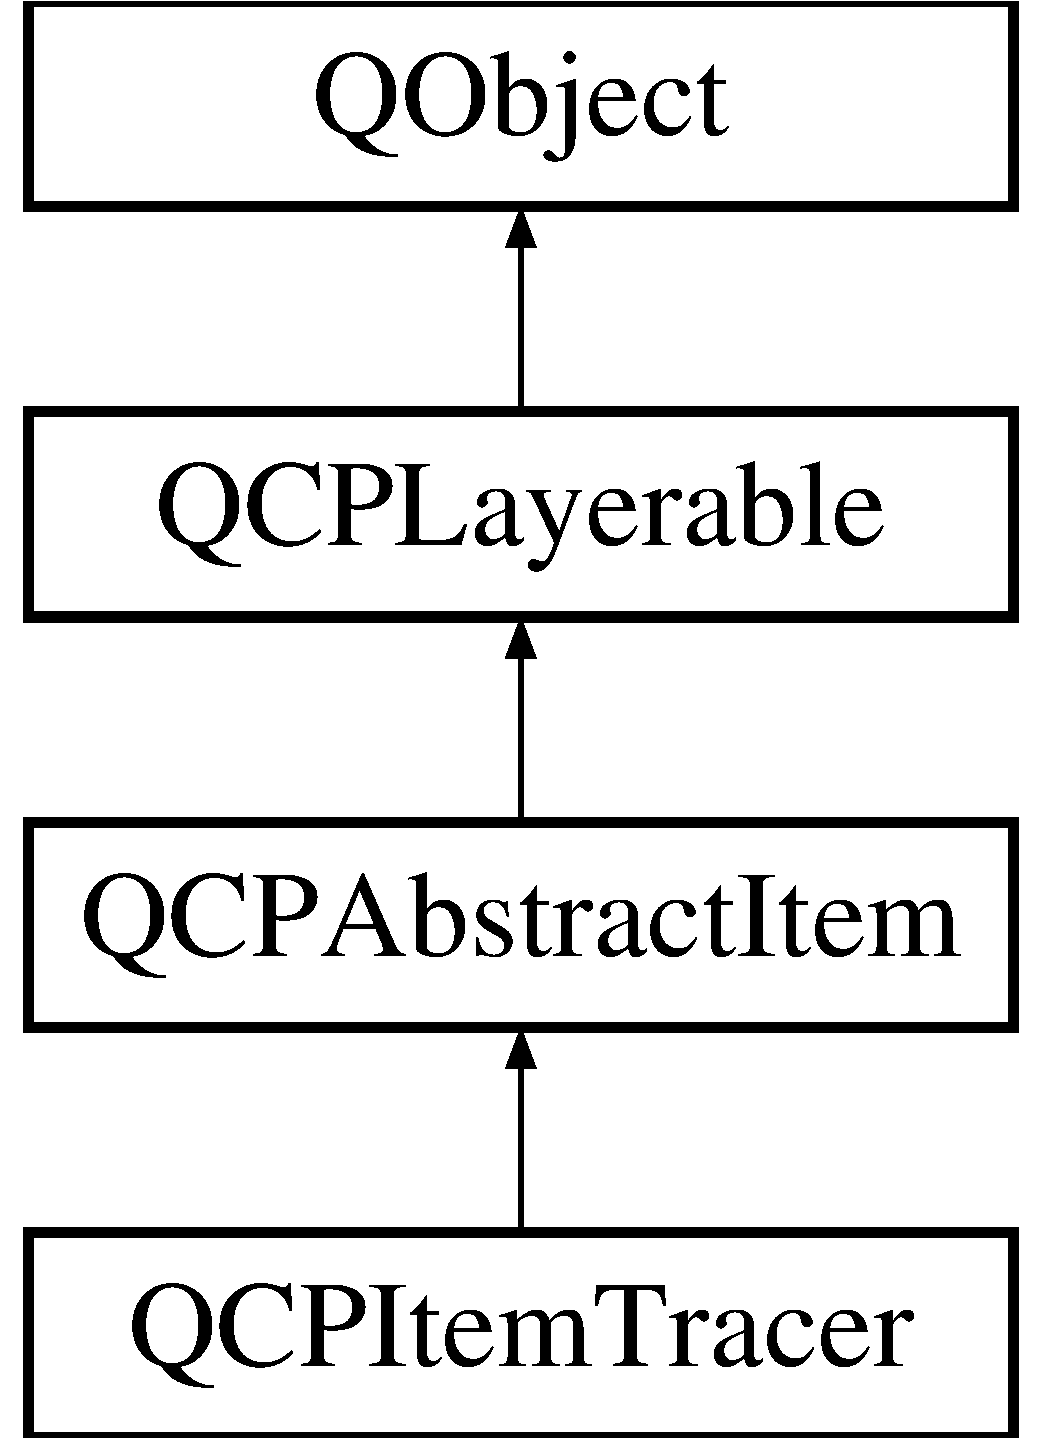
\includegraphics[height=4.000000cm]{class_q_c_p_item_tracer}
\end{center}
\end{figure}
\subsection*{Public Types}
\begin{DoxyCompactItemize}
\item 
enum \hyperlink{class_q_c_p_item_tracer_a2f05ddb13978036f902ca3ab47076500}{Tracer\+Style} \{ \newline
\hyperlink{class_q_c_p_item_tracer_a2f05ddb13978036f902ca3ab47076500aac27462c79146225bfa8fba24d2ee8a4}{ts\+None}, 
\hyperlink{class_q_c_p_item_tracer_a2f05ddb13978036f902ca3ab47076500a3323fb04017146e4885e080a459472fa}{ts\+Plus}, 
\hyperlink{class_q_c_p_item_tracer_a2f05ddb13978036f902ca3ab47076500af562ec81ac3ba99e26ef8540cf1ec16f}{ts\+Crosshair}, 
\hyperlink{class_q_c_p_item_tracer_a2f05ddb13978036f902ca3ab47076500ae2252c28f4842880d71e9f94e69de94e}{ts\+Circle}, 
\newline
\hyperlink{class_q_c_p_item_tracer_a2f05ddb13978036f902ca3ab47076500a4ed5f01f2c5fd86d980366d79f481b9b}{ts\+Square}
 \}
\end{DoxyCompactItemize}
\subsection*{Public Member Functions}
\begin{DoxyCompactItemize}
\item 
\hyperlink{class_q_c_p_item_tracer_adc5ca846eeac323db4aa1fc4081e36be}{Q\+C\+P\+Item\+Tracer} (\hyperlink{class_q_custom_plot}{Q\+Custom\+Plot} $\ast$parent\+Plot)
\item 
\hypertarget{class_q_c_p_item_tracer_a789cdc627868f5a4a0956816072571c9}{}\label{class_q_c_p_item_tracer_a789cdc627868f5a4a0956816072571c9} 
Q\+Pen {\bfseries pen} () const
\item 
\hypertarget{class_q_c_p_item_tracer_ad231a97bac99e01778618d1a5720b17d}{}\label{class_q_c_p_item_tracer_ad231a97bac99e01778618d1a5720b17d} 
Q\+Pen {\bfseries selected\+Pen} () const
\item 
\hypertarget{class_q_c_p_item_tracer_a6dd4660e70f58bb00390bcda56be568d}{}\label{class_q_c_p_item_tracer_a6dd4660e70f58bb00390bcda56be568d} 
Q\+Brush {\bfseries brush} () const
\item 
\hypertarget{class_q_c_p_item_tracer_ae3e48270b4a6ec20f7a9e1f63e778243}{}\label{class_q_c_p_item_tracer_ae3e48270b4a6ec20f7a9e1f63e778243} 
Q\+Brush {\bfseries selected\+Brush} () const
\item 
\hypertarget{class_q_c_p_item_tracer_a4e42d7b49f293273a74a49a2457856e2}{}\label{class_q_c_p_item_tracer_a4e42d7b49f293273a74a49a2457856e2} 
double {\bfseries size} () const
\item 
\hypertarget{class_q_c_p_item_tracer_afdaee32c9ccc9c14502b28d3d86bf5ed}{}\label{class_q_c_p_item_tracer_afdaee32c9ccc9c14502b28d3d86bf5ed} 
\hyperlink{class_q_c_p_item_tracer_a2f05ddb13978036f902ca3ab47076500}{Tracer\+Style} {\bfseries style} () const
\item 
\hypertarget{class_q_c_p_item_tracer_ac6526e3e1fff79894f034823461b138a}{}\label{class_q_c_p_item_tracer_ac6526e3e1fff79894f034823461b138a} 
\hyperlink{class_q_c_p_graph}{Q\+C\+P\+Graph} $\ast$ {\bfseries graph} () const
\item 
\hypertarget{class_q_c_p_item_tracer_ac39a0791109588d11bb97cd643da2470}{}\label{class_q_c_p_item_tracer_ac39a0791109588d11bb97cd643da2470} 
double {\bfseries graph\+Key} () const
\item 
\hypertarget{class_q_c_p_item_tracer_ae9ab6d72e0a35e1769c0b5a9b58181f2}{}\label{class_q_c_p_item_tracer_ae9ab6d72e0a35e1769c0b5a9b58181f2} 
bool {\bfseries interpolating} () const
\item 
void \hyperlink{class_q_c_p_item_tracer_af8048636fc1ef0152e51809b008df2ca}{set\+Pen} (const Q\+Pen \&pen)
\item 
void \hyperlink{class_q_c_p_item_tracer_ae1bf70db7f13f928660168cd3e5069f3}{set\+Selected\+Pen} (const Q\+Pen \&pen)
\item 
void \hyperlink{class_q_c_p_item_tracer_a2c303f7470a30084daa201ed556b3c36}{set\+Brush} (const Q\+Brush \&brush)
\item 
void \hyperlink{class_q_c_p_item_tracer_a0f55c084980a7a312af859d3e7b558ef}{set\+Selected\+Brush} (const Q\+Brush \&brush)
\item 
void \hyperlink{class_q_c_p_item_tracer_ae47fe0617f5fef5fdb766999569be10a}{set\+Size} (double size)
\item 
void \hyperlink{class_q_c_p_item_tracer_a41a2ac4f1acd7897b4e2a2579c03204e}{set\+Style} (\hyperlink{class_q_c_p_item_tracer_a2f05ddb13978036f902ca3ab47076500}{Tracer\+Style} style)
\item 
void \hyperlink{class_q_c_p_item_tracer_af5886f4ded8dd68cb4f3388f390790c0}{set\+Graph} (\hyperlink{class_q_c_p_graph}{Q\+C\+P\+Graph} $\ast$graph)
\item 
void \hyperlink{class_q_c_p_item_tracer_a6840143b42f3b685cedf7c6d83a704c8}{set\+Graph\+Key} (double key)
\item 
void \hyperlink{class_q_c_p_item_tracer_a6c244a9d1175bef12b50afafd4f5fcd2}{set\+Interpolating} (bool enabled)
\item 
virtual double \hyperlink{class_q_c_p_item_tracer_ae1dc728384936184e7552a6d0d67fd75}{select\+Test} (const Q\+PointF \&pos, bool only\+Selectable, Q\+Variant $\ast$details=0) const
\item 
void \hyperlink{class_q_c_p_item_tracer_a5b90296109e36384aedbc8908a670413}{update\+Position} ()
\end{DoxyCompactItemize}
\subsection*{Public Attributes}
\begin{DoxyCompactItemize}
\item 
\hypertarget{class_q_c_p_item_tracer_a69917e2fdb2b3a929c196958feee7cbe}{}\label{class_q_c_p_item_tracer_a69917e2fdb2b3a929c196958feee7cbe} 
\hyperlink{class_q_c_p_item_position}{Q\+C\+P\+Item\+Position} $\ast$const {\bfseries position}
\end{DoxyCompactItemize}
\subsection*{Protected Member Functions}
\begin{DoxyCompactItemize}
\item 
\hypertarget{class_q_c_p_item_tracer_aaaf49b48382c730ec9be0e74c2538315}{}\label{class_q_c_p_item_tracer_aaaf49b48382c730ec9be0e74c2538315} 
virtual void {\bfseries draw} (\hyperlink{class_q_c_p_painter}{Q\+C\+P\+Painter} $\ast$painter)
\item 
\hypertarget{class_q_c_p_item_tracer_abffdcf64d0f84f7b41bd4af07d144642}{}\label{class_q_c_p_item_tracer_abffdcf64d0f84f7b41bd4af07d144642} 
Q\+Pen {\bfseries main\+Pen} () const
\item 
\hypertarget{class_q_c_p_item_tracer_a94f81c54197577e86c53a60cf39155cd}{}\label{class_q_c_p_item_tracer_a94f81c54197577e86c53a60cf39155cd} 
Q\+Brush {\bfseries main\+Brush} () const
\end{DoxyCompactItemize}
\subsection*{Protected Attributes}
\begin{DoxyCompactItemize}
\item 
\hypertarget{class_q_c_p_item_tracer_a579e3bd6bd16d6aaff03638dc8a99a69}{}\label{class_q_c_p_item_tracer_a579e3bd6bd16d6aaff03638dc8a99a69} 
Q\+Pen {\bfseries m\+Pen}
\item 
\hypertarget{class_q_c_p_item_tracer_a3f61829784200819661d1e2a5354d866}{}\label{class_q_c_p_item_tracer_a3f61829784200819661d1e2a5354d866} 
Q\+Pen {\bfseries m\+Selected\+Pen}
\item 
\hypertarget{class_q_c_p_item_tracer_a6597be63a17a266233941354200b2340}{}\label{class_q_c_p_item_tracer_a6597be63a17a266233941354200b2340} 
Q\+Brush {\bfseries m\+Brush}
\item 
\hypertarget{class_q_c_p_item_tracer_a1c15d2adde40efdcc0ef1ff78fd256a6}{}\label{class_q_c_p_item_tracer_a1c15d2adde40efdcc0ef1ff78fd256a6} 
Q\+Brush {\bfseries m\+Selected\+Brush}
\item 
\hypertarget{class_q_c_p_item_tracer_a575153a24bb357d1e006f6bc3bd099b9}{}\label{class_q_c_p_item_tracer_a575153a24bb357d1e006f6bc3bd099b9} 
double {\bfseries m\+Size}
\item 
\hypertarget{class_q_c_p_item_tracer_afb1f236bebf417544e0138fef22a292e}{}\label{class_q_c_p_item_tracer_afb1f236bebf417544e0138fef22a292e} 
\hyperlink{class_q_c_p_item_tracer_a2f05ddb13978036f902ca3ab47076500}{Tracer\+Style} {\bfseries m\+Style}
\item 
\hypertarget{class_q_c_p_item_tracer_a2d70cf616b579563aa15f796dfc143ac}{}\label{class_q_c_p_item_tracer_a2d70cf616b579563aa15f796dfc143ac} 
\hyperlink{class_q_c_p_graph}{Q\+C\+P\+Graph} $\ast$ {\bfseries m\+Graph}
\item 
\hypertarget{class_q_c_p_item_tracer_a8fa20f2e9ee07d21fd7c8d30ba4702ca}{}\label{class_q_c_p_item_tracer_a8fa20f2e9ee07d21fd7c8d30ba4702ca} 
double {\bfseries m\+Graph\+Key}
\item 
\hypertarget{class_q_c_p_item_tracer_afab37c22ad39f235921e86f93cd84595}{}\label{class_q_c_p_item_tracer_afab37c22ad39f235921e86f93cd84595} 
bool {\bfseries m\+Interpolating}
\end{DoxyCompactItemize}
\subsection*{Additional Inherited Members}


\subsection{Detailed Description}
Item that sticks to \hyperlink{class_q_c_p_graph}{Q\+C\+P\+Graph} data points. 

 The tracer can be connected with a \hyperlink{class_q_c_p_graph}{Q\+C\+P\+Graph} via \hyperlink{class_q_c_p_item_tracer_af5886f4ded8dd68cb4f3388f390790c0}{set\+Graph}. Then it will automatically adopt the coordinate axes of the graph and update its {\itshape position} to be on the graph\textquotesingle{}s data. This means the key stays controllable via \hyperlink{class_q_c_p_item_tracer_a6840143b42f3b685cedf7c6d83a704c8}{set\+Graph\+Key}, but the value will follow the graph data. If a \hyperlink{class_q_c_p_graph}{Q\+C\+P\+Graph} is connected, note that setting the coordinates of the tracer item directly via {\itshape position} will have no effect because they will be overriden in the next redraw (this is when the coordinate update happens).

If the specified key in \hyperlink{class_q_c_p_item_tracer_a6840143b42f3b685cedf7c6d83a704c8}{set\+Graph\+Key} is outside the key bounds of the graph, the tracer will stay at the corresponding end of the graph.

With \hyperlink{class_q_c_p_item_tracer_a6c244a9d1175bef12b50afafd4f5fcd2}{set\+Interpolating} you may specify whether the tracer may only stay exactly on data points or whether it interpolates data points linearly, if given a key that lies between two data points of the graph.

The tracer has different visual styles, see \hyperlink{class_q_c_p_item_tracer_a41a2ac4f1acd7897b4e2a2579c03204e}{set\+Style}. It is also possible to make the tracer have no own visual appearance (set the style to \hyperlink{class_q_c_p_item_tracer_a2f05ddb13978036f902ca3ab47076500aac27462c79146225bfa8fba24d2ee8a4}{ts\+None}), and just connect other item positions to the tracer {\itshape position} (used as an anchor) via \hyperlink{class_q_c_p_item_position_ac094d67a95d2dceafa0d50b9db3a7e51}{Q\+C\+P\+Item\+Position\+::set\+Parent\+Anchor}.

\begin{DoxyNote}{Note}
The tracer position is only automatically updated upon redraws. So when the data of the graph changes and immediately afterwards (without a redraw) the a position coordinates of the tracer are retrieved, they will not reflect the updated data of the graph. In this case \hyperlink{class_q_c_p_item_tracer_a5b90296109e36384aedbc8908a670413}{update\+Position} must be called manually, prior to reading the tracer coordinates. 
\end{DoxyNote}


\subsection{Member Enumeration Documentation}
\hypertarget{class_q_c_p_item_tracer_a2f05ddb13978036f902ca3ab47076500}{}\label{class_q_c_p_item_tracer_a2f05ddb13978036f902ca3ab47076500} 
\index{Q\+C\+P\+Item\+Tracer@{Q\+C\+P\+Item\+Tracer}!Tracer\+Style@{Tracer\+Style}}
\index{Tracer\+Style@{Tracer\+Style}!Q\+C\+P\+Item\+Tracer@{Q\+C\+P\+Item\+Tracer}}
\subsubsection{\texorpdfstring{Tracer\+Style}{TracerStyle}}
{\footnotesize\ttfamily enum \hyperlink{class_q_c_p_item_tracer_a2f05ddb13978036f902ca3ab47076500}{Q\+C\+P\+Item\+Tracer\+::\+Tracer\+Style}}

The different visual appearances a tracer item can have. Some styles size may be controlled with \hyperlink{class_q_c_p_item_tracer_ae47fe0617f5fef5fdb766999569be10a}{set\+Size}.

\begin{DoxySeeAlso}{See also}
\hyperlink{class_q_c_p_item_tracer_a41a2ac4f1acd7897b4e2a2579c03204e}{set\+Style} 
\end{DoxySeeAlso}
\begin{DoxyEnumFields}{Enumerator}
\raisebox{\heightof{T}}[0pt][0pt]{\index{ts\+None@{ts\+None}!Q\+C\+P\+Item\+Tracer@{Q\+C\+P\+Item\+Tracer}}\index{Q\+C\+P\+Item\+Tracer@{Q\+C\+P\+Item\+Tracer}!ts\+None@{ts\+None}}}\hypertarget{class_q_c_p_item_tracer_a2f05ddb13978036f902ca3ab47076500aac27462c79146225bfa8fba24d2ee8a4}{}\label{class_q_c_p_item_tracer_a2f05ddb13978036f902ca3ab47076500aac27462c79146225bfa8fba24d2ee8a4} 
ts\+None&The tracer is not visible. \\
\hline

\raisebox{\heightof{T}}[0pt][0pt]{\index{ts\+Plus@{ts\+Plus}!Q\+C\+P\+Item\+Tracer@{Q\+C\+P\+Item\+Tracer}}\index{Q\+C\+P\+Item\+Tracer@{Q\+C\+P\+Item\+Tracer}!ts\+Plus@{ts\+Plus}}}\hypertarget{class_q_c_p_item_tracer_a2f05ddb13978036f902ca3ab47076500a3323fb04017146e4885e080a459472fa}{}\label{class_q_c_p_item_tracer_a2f05ddb13978036f902ca3ab47076500a3323fb04017146e4885e080a459472fa} 
ts\+Plus&A plus shaped crosshair with limited size. \\
\hline

\raisebox{\heightof{T}}[0pt][0pt]{\index{ts\+Crosshair@{ts\+Crosshair}!Q\+C\+P\+Item\+Tracer@{Q\+C\+P\+Item\+Tracer}}\index{Q\+C\+P\+Item\+Tracer@{Q\+C\+P\+Item\+Tracer}!ts\+Crosshair@{ts\+Crosshair}}}\hypertarget{class_q_c_p_item_tracer_a2f05ddb13978036f902ca3ab47076500af562ec81ac3ba99e26ef8540cf1ec16f}{}\label{class_q_c_p_item_tracer_a2f05ddb13978036f902ca3ab47076500af562ec81ac3ba99e26ef8540cf1ec16f} 
ts\+Crosshair&A plus shaped crosshair which spans the complete axis rect. \\
\hline

\raisebox{\heightof{T}}[0pt][0pt]{\index{ts\+Circle@{ts\+Circle}!Q\+C\+P\+Item\+Tracer@{Q\+C\+P\+Item\+Tracer}}\index{Q\+C\+P\+Item\+Tracer@{Q\+C\+P\+Item\+Tracer}!ts\+Circle@{ts\+Circle}}}\hypertarget{class_q_c_p_item_tracer_a2f05ddb13978036f902ca3ab47076500ae2252c28f4842880d71e9f94e69de94e}{}\label{class_q_c_p_item_tracer_a2f05ddb13978036f902ca3ab47076500ae2252c28f4842880d71e9f94e69de94e} 
ts\+Circle&A circle. \\
\hline

\raisebox{\heightof{T}}[0pt][0pt]{\index{ts\+Square@{ts\+Square}!Q\+C\+P\+Item\+Tracer@{Q\+C\+P\+Item\+Tracer}}\index{Q\+C\+P\+Item\+Tracer@{Q\+C\+P\+Item\+Tracer}!ts\+Square@{ts\+Square}}}\hypertarget{class_q_c_p_item_tracer_a2f05ddb13978036f902ca3ab47076500a4ed5f01f2c5fd86d980366d79f481b9b}{}\label{class_q_c_p_item_tracer_a2f05ddb13978036f902ca3ab47076500a4ed5f01f2c5fd86d980366d79f481b9b} 
ts\+Square&A square. \\
\hline

\end{DoxyEnumFields}


\subsection{Constructor \& Destructor Documentation}
\hypertarget{class_q_c_p_item_tracer_adc5ca846eeac323db4aa1fc4081e36be}{}\label{class_q_c_p_item_tracer_adc5ca846eeac323db4aa1fc4081e36be} 
\index{Q\+C\+P\+Item\+Tracer@{Q\+C\+P\+Item\+Tracer}!Q\+C\+P\+Item\+Tracer@{Q\+C\+P\+Item\+Tracer}}
\index{Q\+C\+P\+Item\+Tracer@{Q\+C\+P\+Item\+Tracer}!Q\+C\+P\+Item\+Tracer@{Q\+C\+P\+Item\+Tracer}}
\subsubsection{\texorpdfstring{Q\+C\+P\+Item\+Tracer()}{QCPItemTracer()}}
{\footnotesize\ttfamily Q\+C\+P\+Item\+Tracer\+::\+Q\+C\+P\+Item\+Tracer (\begin{DoxyParamCaption}\item[{\hyperlink{class_q_custom_plot}{Q\+Custom\+Plot} $\ast$}]{parent\+Plot }\end{DoxyParamCaption})}

Creates a tracer item and sets default values.

The constructed item can be added to the plot with \hyperlink{class_q_custom_plot_aa500620379262321685cb7a7674cbd2a}{Q\+Custom\+Plot\+::add\+Item}. 

\subsection{Member Function Documentation}
\hypertarget{class_q_c_p_item_tracer_ae1dc728384936184e7552a6d0d67fd75}{}\label{class_q_c_p_item_tracer_ae1dc728384936184e7552a6d0d67fd75} 
\index{Q\+C\+P\+Item\+Tracer@{Q\+C\+P\+Item\+Tracer}!select\+Test@{select\+Test}}
\index{select\+Test@{select\+Test}!Q\+C\+P\+Item\+Tracer@{Q\+C\+P\+Item\+Tracer}}
\subsubsection{\texorpdfstring{select\+Test()}{selectTest()}}
{\footnotesize\ttfamily double Q\+C\+P\+Item\+Tracer\+::select\+Test (\begin{DoxyParamCaption}\item[{const Q\+PointF \&}]{pos,  }\item[{bool}]{only\+Selectable,  }\item[{Q\+Variant $\ast$}]{details = {\ttfamily 0} }\end{DoxyParamCaption}) const\hspace{0.3cm}{\ttfamily [virtual]}}

This function is used to decide whether a click hits a layerable object or not.

{\itshape pos} is a point in pixel coordinates on the \hyperlink{class_q_custom_plot}{Q\+Custom\+Plot} surface. This function returns the shortest pixel distance of this point to the object. If the object is either invisible or the distance couldn\textquotesingle{}t be determined, -\/1.\+0 is returned. Further, if {\itshape only\+Selectable} is true and the object is not selectable, -\/1.\+0 is returned, too.

If the object is represented not by single lines but by an area like a \hyperlink{class_q_c_p_item_text}{Q\+C\+P\+Item\+Text} or the bars of a \hyperlink{class_q_c_p_bars}{Q\+C\+P\+Bars} plottable, a click inside the area should also be considered a hit. In these cases this function thus returns a constant value greater zero but still below the parent plot\textquotesingle{}s selection tolerance. (typically the selection\+Tolerance multiplied by 0.\+99).

Providing a constant value for area objects allows selecting line objects even when they are obscured by such area objects, by clicking close to the lines (i.\+e. closer than 0.\+99$\ast$selection\+Tolerance).

The actual setting of the selection state is not done by this function. This is handled by the parent \hyperlink{class_q_custom_plot}{Q\+Custom\+Plot} when the mouse\+Release\+Event occurs, and the finally selected object is notified via the select\+Event/deselect\+Event methods.

{\itshape details} is an optional output parameter. Every layerable subclass may place any information in {\itshape details}. This information will be passed to select\+Event when the parent \hyperlink{class_q_custom_plot}{Q\+Custom\+Plot} decides on the basis of this select\+Test call, that the object was successfully selected. The subsequent call to select\+Event will carry the {\itshape details}. This is useful for multi-\/part objects (like \hyperlink{class_q_c_p_axis}{Q\+C\+P\+Axis}). This way, a possibly complex calculation to decide which part was clicked is only done once in \hyperlink{class_q_c_p_item_tracer_ae1dc728384936184e7552a6d0d67fd75}{select\+Test}. The result (i.\+e. the actually clicked part) can then be placed in {\itshape details}. So in the subsequent select\+Event, the decision which part was selected doesn\textquotesingle{}t have to be done a second time for a single selection operation.

You may pass 0 as {\itshape details} to indicate that you are not interested in those selection details.

\begin{DoxySeeAlso}{See also}
select\+Event, deselect\+Event, \hyperlink{class_q_custom_plot_a5ee1e2f6ae27419deca53e75907c27e5}{Q\+Custom\+Plot\+::set\+Interactions} 
\end{DoxySeeAlso}


Implements \hyperlink{class_q_c_p_abstract_item_a96d522d10ffc0413b9a366c6f7f0476b}{Q\+C\+P\+Abstract\+Item}.

\hypertarget{class_q_c_p_item_tracer_a2c303f7470a30084daa201ed556b3c36}{}\label{class_q_c_p_item_tracer_a2c303f7470a30084daa201ed556b3c36} 
\index{Q\+C\+P\+Item\+Tracer@{Q\+C\+P\+Item\+Tracer}!set\+Brush@{set\+Brush}}
\index{set\+Brush@{set\+Brush}!Q\+C\+P\+Item\+Tracer@{Q\+C\+P\+Item\+Tracer}}
\subsubsection{\texorpdfstring{set\+Brush()}{setBrush()}}
{\footnotesize\ttfamily void Q\+C\+P\+Item\+Tracer\+::set\+Brush (\begin{DoxyParamCaption}\item[{const Q\+Brush \&}]{brush }\end{DoxyParamCaption})}

Sets the brush that will be used to draw any fills of the tracer

\begin{DoxySeeAlso}{See also}
\hyperlink{class_q_c_p_item_tracer_a0f55c084980a7a312af859d3e7b558ef}{set\+Selected\+Brush}, \hyperlink{class_q_c_p_item_tracer_af8048636fc1ef0152e51809b008df2ca}{set\+Pen} 
\end{DoxySeeAlso}
\hypertarget{class_q_c_p_item_tracer_af5886f4ded8dd68cb4f3388f390790c0}{}\label{class_q_c_p_item_tracer_af5886f4ded8dd68cb4f3388f390790c0} 
\index{Q\+C\+P\+Item\+Tracer@{Q\+C\+P\+Item\+Tracer}!set\+Graph@{set\+Graph}}
\index{set\+Graph@{set\+Graph}!Q\+C\+P\+Item\+Tracer@{Q\+C\+P\+Item\+Tracer}}
\subsubsection{\texorpdfstring{set\+Graph()}{setGraph()}}
{\footnotesize\ttfamily void Q\+C\+P\+Item\+Tracer\+::set\+Graph (\begin{DoxyParamCaption}\item[{\hyperlink{class_q_c_p_graph}{Q\+C\+P\+Graph} $\ast$}]{graph }\end{DoxyParamCaption})}

Sets the \hyperlink{class_q_c_p_graph}{Q\+C\+P\+Graph} this tracer sticks to. The tracer {\itshape position} will be set to type \hyperlink{class_q_c_p_item_position_aad9936c22bf43e3d358552f6e86dbdc8ad5ffb8dc99ad73263f7010c77342294c}{Q\+C\+P\+Item\+Position\+::pt\+Plot\+Coords} and the axes will be set to the axes of {\itshape graph}.

To free the tracer from any graph, set {\itshape graph} to 0. The tracer {\itshape position} can then be placed freely like any other item position. This is the state the tracer will assume when its graph gets deleted while still attached to it.

\begin{DoxySeeAlso}{See also}
\hyperlink{class_q_c_p_item_tracer_a6840143b42f3b685cedf7c6d83a704c8}{set\+Graph\+Key} 
\end{DoxySeeAlso}
\hypertarget{class_q_c_p_item_tracer_a6840143b42f3b685cedf7c6d83a704c8}{}\label{class_q_c_p_item_tracer_a6840143b42f3b685cedf7c6d83a704c8} 
\index{Q\+C\+P\+Item\+Tracer@{Q\+C\+P\+Item\+Tracer}!set\+Graph\+Key@{set\+Graph\+Key}}
\index{set\+Graph\+Key@{set\+Graph\+Key}!Q\+C\+P\+Item\+Tracer@{Q\+C\+P\+Item\+Tracer}}
\subsubsection{\texorpdfstring{set\+Graph\+Key()}{setGraphKey()}}
{\footnotesize\ttfamily void Q\+C\+P\+Item\+Tracer\+::set\+Graph\+Key (\begin{DoxyParamCaption}\item[{double}]{key }\end{DoxyParamCaption})}

Sets the key of the graph\textquotesingle{}s data point the tracer will be positioned at. This is the only free coordinate of a tracer when attached to a graph.

Depending on \hyperlink{class_q_c_p_item_tracer_a6c244a9d1175bef12b50afafd4f5fcd2}{set\+Interpolating}, the tracer will be either positioned on the data point closest to {\itshape key}, or will stay exactly at {\itshape key} and interpolate the value linearly.

\begin{DoxySeeAlso}{See also}
\hyperlink{class_q_c_p_item_tracer_af5886f4ded8dd68cb4f3388f390790c0}{set\+Graph}, \hyperlink{class_q_c_p_item_tracer_a6c244a9d1175bef12b50afafd4f5fcd2}{set\+Interpolating} 
\end{DoxySeeAlso}
\hypertarget{class_q_c_p_item_tracer_a6c244a9d1175bef12b50afafd4f5fcd2}{}\label{class_q_c_p_item_tracer_a6c244a9d1175bef12b50afafd4f5fcd2} 
\index{Q\+C\+P\+Item\+Tracer@{Q\+C\+P\+Item\+Tracer}!set\+Interpolating@{set\+Interpolating}}
\index{set\+Interpolating@{set\+Interpolating}!Q\+C\+P\+Item\+Tracer@{Q\+C\+P\+Item\+Tracer}}
\subsubsection{\texorpdfstring{set\+Interpolating()}{setInterpolating()}}
{\footnotesize\ttfamily void Q\+C\+P\+Item\+Tracer\+::set\+Interpolating (\begin{DoxyParamCaption}\item[{bool}]{enabled }\end{DoxyParamCaption})}

Sets whether the value of the graph\textquotesingle{}s data points shall be interpolated, when positioning the tracer.

If {\itshape enabled} is set to false and a key is given with \hyperlink{class_q_c_p_item_tracer_a6840143b42f3b685cedf7c6d83a704c8}{set\+Graph\+Key}, the tracer is placed on the data point of the graph which is closest to the key, but which is not necessarily exactly there. If {\itshape enabled} is true, the tracer will be positioned exactly at the specified key, and the appropriate value will be interpolated from the graph\textquotesingle{}s data points linearly.

\begin{DoxySeeAlso}{See also}
\hyperlink{class_q_c_p_item_tracer_af5886f4ded8dd68cb4f3388f390790c0}{set\+Graph}, \hyperlink{class_q_c_p_item_tracer_a6840143b42f3b685cedf7c6d83a704c8}{set\+Graph\+Key} 
\end{DoxySeeAlso}
\hypertarget{class_q_c_p_item_tracer_af8048636fc1ef0152e51809b008df2ca}{}\label{class_q_c_p_item_tracer_af8048636fc1ef0152e51809b008df2ca} 
\index{Q\+C\+P\+Item\+Tracer@{Q\+C\+P\+Item\+Tracer}!set\+Pen@{set\+Pen}}
\index{set\+Pen@{set\+Pen}!Q\+C\+P\+Item\+Tracer@{Q\+C\+P\+Item\+Tracer}}
\subsubsection{\texorpdfstring{set\+Pen()}{setPen()}}
{\footnotesize\ttfamily void Q\+C\+P\+Item\+Tracer\+::set\+Pen (\begin{DoxyParamCaption}\item[{const Q\+Pen \&}]{pen }\end{DoxyParamCaption})}

Sets the pen that will be used to draw the line of the tracer

\begin{DoxySeeAlso}{See also}
\hyperlink{class_q_c_p_item_tracer_ae1bf70db7f13f928660168cd3e5069f3}{set\+Selected\+Pen}, \hyperlink{class_q_c_p_item_tracer_a2c303f7470a30084daa201ed556b3c36}{set\+Brush} 
\end{DoxySeeAlso}
\hypertarget{class_q_c_p_item_tracer_a0f55c084980a7a312af859d3e7b558ef}{}\label{class_q_c_p_item_tracer_a0f55c084980a7a312af859d3e7b558ef} 
\index{Q\+C\+P\+Item\+Tracer@{Q\+C\+P\+Item\+Tracer}!set\+Selected\+Brush@{set\+Selected\+Brush}}
\index{set\+Selected\+Brush@{set\+Selected\+Brush}!Q\+C\+P\+Item\+Tracer@{Q\+C\+P\+Item\+Tracer}}
\subsubsection{\texorpdfstring{set\+Selected\+Brush()}{setSelectedBrush()}}
{\footnotesize\ttfamily void Q\+C\+P\+Item\+Tracer\+::set\+Selected\+Brush (\begin{DoxyParamCaption}\item[{const Q\+Brush \&}]{brush }\end{DoxyParamCaption})}

Sets the brush that will be used to draw any fills of the tracer, when selected.

\begin{DoxySeeAlso}{See also}
\hyperlink{class_q_c_p_item_tracer_a2c303f7470a30084daa201ed556b3c36}{set\+Brush}, \hyperlink{class_q_c_p_abstract_item_a203de94ad586cc44d16c9565f49d3378}{set\+Selected} 
\end{DoxySeeAlso}
\hypertarget{class_q_c_p_item_tracer_ae1bf70db7f13f928660168cd3e5069f3}{}\label{class_q_c_p_item_tracer_ae1bf70db7f13f928660168cd3e5069f3} 
\index{Q\+C\+P\+Item\+Tracer@{Q\+C\+P\+Item\+Tracer}!set\+Selected\+Pen@{set\+Selected\+Pen}}
\index{set\+Selected\+Pen@{set\+Selected\+Pen}!Q\+C\+P\+Item\+Tracer@{Q\+C\+P\+Item\+Tracer}}
\subsubsection{\texorpdfstring{set\+Selected\+Pen()}{setSelectedPen()}}
{\footnotesize\ttfamily void Q\+C\+P\+Item\+Tracer\+::set\+Selected\+Pen (\begin{DoxyParamCaption}\item[{const Q\+Pen \&}]{pen }\end{DoxyParamCaption})}

Sets the pen that will be used to draw the line of the tracer when selected

\begin{DoxySeeAlso}{See also}
\hyperlink{class_q_c_p_item_tracer_af8048636fc1ef0152e51809b008df2ca}{set\+Pen}, \hyperlink{class_q_c_p_abstract_item_a203de94ad586cc44d16c9565f49d3378}{set\+Selected} 
\end{DoxySeeAlso}
\hypertarget{class_q_c_p_item_tracer_ae47fe0617f5fef5fdb766999569be10a}{}\label{class_q_c_p_item_tracer_ae47fe0617f5fef5fdb766999569be10a} 
\index{Q\+C\+P\+Item\+Tracer@{Q\+C\+P\+Item\+Tracer}!set\+Size@{set\+Size}}
\index{set\+Size@{set\+Size}!Q\+C\+P\+Item\+Tracer@{Q\+C\+P\+Item\+Tracer}}
\subsubsection{\texorpdfstring{set\+Size()}{setSize()}}
{\footnotesize\ttfamily void Q\+C\+P\+Item\+Tracer\+::set\+Size (\begin{DoxyParamCaption}\item[{double}]{size }\end{DoxyParamCaption})}

Sets the size of the tracer in pixels, if the style supports setting a size (e.\+g. \hyperlink{class_q_c_p_item_tracer_a2f05ddb13978036f902ca3ab47076500a4ed5f01f2c5fd86d980366d79f481b9b}{ts\+Square} does, \hyperlink{class_q_c_p_item_tracer_a2f05ddb13978036f902ca3ab47076500af562ec81ac3ba99e26ef8540cf1ec16f}{ts\+Crosshair} does not). \hypertarget{class_q_c_p_item_tracer_a41a2ac4f1acd7897b4e2a2579c03204e}{}\label{class_q_c_p_item_tracer_a41a2ac4f1acd7897b4e2a2579c03204e} 
\index{Q\+C\+P\+Item\+Tracer@{Q\+C\+P\+Item\+Tracer}!set\+Style@{set\+Style}}
\index{set\+Style@{set\+Style}!Q\+C\+P\+Item\+Tracer@{Q\+C\+P\+Item\+Tracer}}
\subsubsection{\texorpdfstring{set\+Style()}{setStyle()}}
{\footnotesize\ttfamily void Q\+C\+P\+Item\+Tracer\+::set\+Style (\begin{DoxyParamCaption}\item[{\hyperlink{class_q_c_p_item_tracer_a2f05ddb13978036f902ca3ab47076500}{Q\+C\+P\+Item\+Tracer\+::\+Tracer\+Style}}]{style }\end{DoxyParamCaption})}

Sets the style/visual appearance of the tracer.

If you only want to use the tracer {\itshape position} as an anchor for other items, set {\itshape style} to \hyperlink{class_q_c_p_item_tracer_a2f05ddb13978036f902ca3ab47076500aac27462c79146225bfa8fba24d2ee8a4}{ts\+None}. \hypertarget{class_q_c_p_item_tracer_a5b90296109e36384aedbc8908a670413}{}\label{class_q_c_p_item_tracer_a5b90296109e36384aedbc8908a670413} 
\index{Q\+C\+P\+Item\+Tracer@{Q\+C\+P\+Item\+Tracer}!update\+Position@{update\+Position}}
\index{update\+Position@{update\+Position}!Q\+C\+P\+Item\+Tracer@{Q\+C\+P\+Item\+Tracer}}
\subsubsection{\texorpdfstring{update\+Position()}{updatePosition()}}
{\footnotesize\ttfamily void Q\+C\+P\+Item\+Tracer\+::update\+Position (\begin{DoxyParamCaption}{ }\end{DoxyParamCaption})}

If the tracer is connected with a graph (\hyperlink{class_q_c_p_item_tracer_af5886f4ded8dd68cb4f3388f390790c0}{set\+Graph}), this function updates the tracer\textquotesingle{}s {\itshape position} to reside on the graph data, depending on the configured key (\hyperlink{class_q_c_p_item_tracer_a6840143b42f3b685cedf7c6d83a704c8}{set\+Graph\+Key}).

It is called automatically on every redraw and normally doesn\textquotesingle{}t need to be called manually. One exception is when you want to read the tracer coordinates via {\itshape position} and are not sure that the graph\textquotesingle{}s data (or the tracer key with \hyperlink{class_q_c_p_item_tracer_a6840143b42f3b685cedf7c6d83a704c8}{set\+Graph\+Key}) hasn\textquotesingle{}t changed since the last redraw. In that situation, call this function before accessing {\itshape position}, to make sure you don\textquotesingle{}t get out-\/of-\/date coordinates.

If there is no graph set on this tracer, this function does nothing. 

The documentation for this class was generated from the following files\+:\begin{DoxyCompactItemize}
\item 
F\+E\+S\+S-\/\+G\+U\+I/\hyperlink{qcustomplot_8h}{qcustomplot.\+h}\item 
F\+E\+S\+S-\/\+G\+U\+I/\hyperlink{qcustomplot_8cpp}{qcustomplot.\+cpp}\end{DoxyCompactItemize}

\hypertarget{class_q_c_p_layer}{}\section{Q\+C\+P\+Layer Class Reference}
\label{class_q_c_p_layer}\index{Q\+C\+P\+Layer@{Q\+C\+P\+Layer}}


A layer that may contain objects, to control the rendering order.  


Inheritance diagram for Q\+C\+P\+Layer\+:\begin{figure}[H]
\begin{center}
\leavevmode
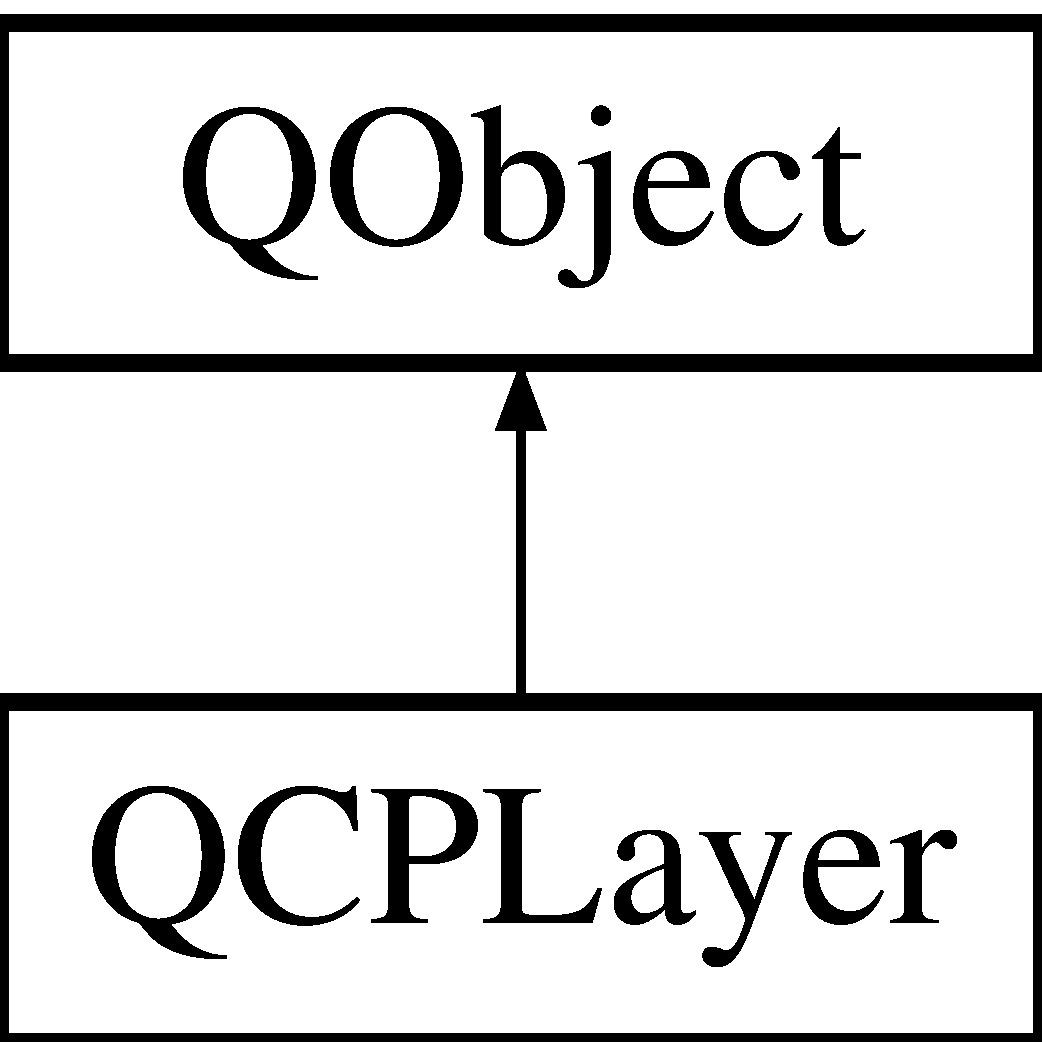
\includegraphics[height=2.000000cm]{class_q_c_p_layer}
\end{center}
\end{figure}
\subsection*{Public Member Functions}
\begin{DoxyCompactItemize}
\item 
\hyperlink{class_q_c_p_layer_a5d0657fc86d624e5efbe930ef21af718}{Q\+C\+P\+Layer} (\hyperlink{class_q_custom_plot}{Q\+Custom\+Plot} $\ast$parent\+Plot, const Q\+String \&layer\+Name)
\item 
\hypertarget{class_q_c_p_layer_a5520019787482e13857ebe631c27c3fa}{}\label{class_q_c_p_layer_a5520019787482e13857ebe631c27c3fa} 
\hyperlink{class_q_custom_plot}{Q\+Custom\+Plot} $\ast$ {\bfseries parent\+Plot} () const
\item 
\hypertarget{class_q_c_p_layer_a37806f662b50b588fb1029a14fc5ef50}{}\label{class_q_c_p_layer_a37806f662b50b588fb1029a14fc5ef50} 
Q\+String {\bfseries name} () const
\item 
int \hyperlink{class_q_c_p_layer_ad322905c4700dcc7ceba63e011c730d2}{index} () const
\item 
Q\+List$<$ \hyperlink{class_q_c_p_layerable}{Q\+C\+P\+Layerable} $\ast$ $>$ \hyperlink{class_q_c_p_layer_a183b90941fc78f0b136edd77c5fb6966}{children} () const
\item 
\hypertarget{class_q_c_p_layer_ad1cc2d6b32d2abb33c7f449b964e068c}{}\label{class_q_c_p_layer_ad1cc2d6b32d2abb33c7f449b964e068c} 
bool {\bfseries visible} () const
\item 
void \hyperlink{class_q_c_p_layer_ac07671f74edf6884b51a82afb2c19516}{set\+Visible} (bool visible)
\end{DoxyCompactItemize}
\subsection*{Protected Member Functions}
\begin{DoxyCompactItemize}
\item 
\hypertarget{class_q_c_p_layer_a57ce5e49364aa9122276d5df3b4a0ddc}{}\label{class_q_c_p_layer_a57ce5e49364aa9122276d5df3b4a0ddc} 
void {\bfseries add\+Child} (\hyperlink{class_q_c_p_layerable}{Q\+C\+P\+Layerable} $\ast$layerable, bool prepend)
\item 
\hypertarget{class_q_c_p_layer_ac2f64ac7761650582d968d86670ef362}{}\label{class_q_c_p_layer_ac2f64ac7761650582d968d86670ef362} 
void {\bfseries remove\+Child} (\hyperlink{class_q_c_p_layerable}{Q\+C\+P\+Layerable} $\ast$layerable)
\end{DoxyCompactItemize}
\subsection*{Protected Attributes}
\begin{DoxyCompactItemize}
\item 
\hypertarget{class_q_c_p_layer_a2f3374a7884bf403720cd1cf6f7ad1bb}{}\label{class_q_c_p_layer_a2f3374a7884bf403720cd1cf6f7ad1bb} 
\hyperlink{class_q_custom_plot}{Q\+Custom\+Plot} $\ast$ {\bfseries m\+Parent\+Plot}
\item 
\hypertarget{class_q_c_p_layer_a91e6298183cb4b9dfd4efdfaf1ecc220}{}\label{class_q_c_p_layer_a91e6298183cb4b9dfd4efdfaf1ecc220} 
Q\+String {\bfseries m\+Name}
\item 
\hypertarget{class_q_c_p_layer_a122088bcab6cec76a52b75ce8606605b}{}\label{class_q_c_p_layer_a122088bcab6cec76a52b75ce8606605b} 
int {\bfseries m\+Index}
\item 
\hypertarget{class_q_c_p_layer_a704aa71bba469383c3a3c598c1ec0d28}{}\label{class_q_c_p_layer_a704aa71bba469383c3a3c598c1ec0d28} 
Q\+List$<$ \hyperlink{class_q_c_p_layerable}{Q\+C\+P\+Layerable} $\ast$ $>$ {\bfseries m\+Children}
\item 
\hypertarget{class_q_c_p_layer_a264950deb08e589460c126c895a1e2b5}{}\label{class_q_c_p_layer_a264950deb08e589460c126c895a1e2b5} 
bool {\bfseries m\+Visible}
\end{DoxyCompactItemize}
\subsection*{Friends}
\begin{DoxyCompactItemize}
\item 
\hypertarget{class_q_c_p_layer_a1cdf9df76adcfae45261690aa0ca2198}{}\label{class_q_c_p_layer_a1cdf9df76adcfae45261690aa0ca2198} 
class {\bfseries Q\+Custom\+Plot}
\item 
\hypertarget{class_q_c_p_layer_ad655f55cccf49ba14d5172ec517e07ae}{}\label{class_q_c_p_layer_ad655f55cccf49ba14d5172ec517e07ae} 
class {\bfseries Q\+C\+P\+Layerable}
\end{DoxyCompactItemize}


\subsection{Detailed Description}
A layer that may contain objects, to control the rendering order. 

The Layering system of \hyperlink{class_q_custom_plot}{Q\+Custom\+Plot} is the mechanism to control the rendering order of the elements inside the plot.

It is based on the two classes \hyperlink{class_q_c_p_layer}{Q\+C\+P\+Layer} and \hyperlink{class_q_c_p_layerable}{Q\+C\+P\+Layerable}. \hyperlink{class_q_custom_plot}{Q\+Custom\+Plot} holds an ordered list of one or more instances of \hyperlink{class_q_c_p_layer}{Q\+C\+P\+Layer} (see \hyperlink{class_q_custom_plot_ad5255393df078448bb6ac83fa5db5f52}{Q\+Custom\+Plot\+::add\+Layer}, \hyperlink{class_q_custom_plot_a0a96244e7773b242ef23c32b7bdfb159}{Q\+Custom\+Plot\+::layer}, \hyperlink{class_q_custom_plot_ae896140beff19424e9e9e02d6e331104}{Q\+Custom\+Plot\+::move\+Layer}, etc.). When replotting, \hyperlink{class_q_custom_plot}{Q\+Custom\+Plot} goes through the list of layers bottom to top and successively draws the layerables of the layers.

A \hyperlink{class_q_c_p_layer}{Q\+C\+P\+Layer} contains an ordered list of \hyperlink{class_q_c_p_layerable}{Q\+C\+P\+Layerable} instances. \hyperlink{class_q_c_p_layerable}{Q\+C\+P\+Layerable} is an abstract base class from which almost all visible objects derive, like axes, grids, graphs, items, etc.

Initially, \hyperlink{class_q_custom_plot}{Q\+Custom\+Plot} has five layers\+: \char`\"{}background\char`\"{}, \char`\"{}grid\char`\"{}, \char`\"{}main\char`\"{}, \char`\"{}axes\char`\"{} and \char`\"{}legend\char`\"{} (in that order). The top two layers \char`\"{}axes\char`\"{} and \char`\"{}legend\char`\"{} contain the default axes and legend, so they will be drawn on top. In the middle, there is the \char`\"{}main\char`\"{} layer. It is initially empty and set as the current layer (see \hyperlink{class_q_custom_plot_a73a6dc47c653bb6f8f030abca5a11852}{Q\+Custom\+Plot\+::set\+Current\+Layer}). This means, all new plottables, items etc. are created on this layer by default. Then comes the \char`\"{}grid\char`\"{} layer which contains the \hyperlink{class_q_c_p_grid}{Q\+C\+P\+Grid} instances (which belong tightly to \hyperlink{class_q_c_p_axis}{Q\+C\+P\+Axis}, see \hyperlink{class_q_c_p_axis_a63f1dd2df663680d2a8d06c19592dd63}{Q\+C\+P\+Axis\+::grid}). The Axis rect background shall be drawn behind everything else, thus the default \hyperlink{class_q_c_p_axis_rect}{Q\+C\+P\+Axis\+Rect} instance is placed on the \char`\"{}background\char`\"{} layer. Of course, the layer affiliation of the individual objects can be changed as required (\hyperlink{class_q_c_p_layerable_ab0d0da6d2de45a118886d2c8e16d5a54}{Q\+C\+P\+Layerable\+::set\+Layer}).

Controlling the ordering of objects is easy\+: Create a new layer in the position you want it to be, e.\+g. above \char`\"{}main\char`\"{}, with \hyperlink{class_q_custom_plot_ad5255393df078448bb6ac83fa5db5f52}{Q\+Custom\+Plot\+::add\+Layer}. Then set the current layer with \hyperlink{class_q_custom_plot_a73a6dc47c653bb6f8f030abca5a11852}{Q\+Custom\+Plot\+::set\+Current\+Layer} to that new layer and finally create the objects normally. They will be placed on the new layer automatically, due to the current layer setting. Alternatively you could have also ignored the current layer setting and just moved the objects with \hyperlink{class_q_c_p_layerable_ab0d0da6d2de45a118886d2c8e16d5a54}{Q\+C\+P\+Layerable\+::set\+Layer} to the desired layer after creating them.

It is also possible to move whole layers. For example, If you want the grid to be shown in front of all plottables/items on the \char`\"{}main\char`\"{} layer, just move it above \char`\"{}main\char`\"{} with \hyperlink{class_q_custom_plot_ae896140beff19424e9e9e02d6e331104}{Q\+Custom\+Plot\+::move\+Layer}.

The rendering order within one layer is simply by order of creation or insertion. The item created last (or added last to the layer), is drawn on top of all other objects on that layer.

When a layer is deleted, the objects on it are not deleted with it, but fall on the layer below the deleted layer, see \hyperlink{class_q_custom_plot_a40f75e342c5eaab6a86066a42a0e2a94}{Q\+Custom\+Plot\+::remove\+Layer}. 

\subsection{Constructor \& Destructor Documentation}
\hypertarget{class_q_c_p_layer_a5d0657fc86d624e5efbe930ef21af718}{}\label{class_q_c_p_layer_a5d0657fc86d624e5efbe930ef21af718} 
\index{Q\+C\+P\+Layer@{Q\+C\+P\+Layer}!Q\+C\+P\+Layer@{Q\+C\+P\+Layer}}
\index{Q\+C\+P\+Layer@{Q\+C\+P\+Layer}!Q\+C\+P\+Layer@{Q\+C\+P\+Layer}}
\subsubsection{\texorpdfstring{Q\+C\+P\+Layer()}{QCPLayer()}}
{\footnotesize\ttfamily Q\+C\+P\+Layer\+::\+Q\+C\+P\+Layer (\begin{DoxyParamCaption}\item[{\hyperlink{class_q_custom_plot}{Q\+Custom\+Plot} $\ast$}]{parent\+Plot,  }\item[{const Q\+String \&}]{layer\+Name }\end{DoxyParamCaption})}

Creates a new \hyperlink{class_q_c_p_layer}{Q\+C\+P\+Layer} instance.

Normally you shouldn\textquotesingle{}t directly instantiate layers, use \hyperlink{class_q_custom_plot_ad5255393df078448bb6ac83fa5db5f52}{Q\+Custom\+Plot\+::add\+Layer} instead.

\begin{DoxyWarning}{Warning}
It is not checked that {\itshape layer\+Name} is actually a unique layer name in {\itshape parent\+Plot}. This check is only performed by \hyperlink{class_q_custom_plot_ad5255393df078448bb6ac83fa5db5f52}{Q\+Custom\+Plot\+::add\+Layer}. 
\end{DoxyWarning}


\subsection{Member Function Documentation}
\hypertarget{class_q_c_p_layer_a183b90941fc78f0b136edd77c5fb6966}{}\label{class_q_c_p_layer_a183b90941fc78f0b136edd77c5fb6966} 
\index{Q\+C\+P\+Layer@{Q\+C\+P\+Layer}!children@{children}}
\index{children@{children}!Q\+C\+P\+Layer@{Q\+C\+P\+Layer}}
\subsubsection{\texorpdfstring{children()}{children()}}
{\footnotesize\ttfamily Q\+List$<$ \hyperlink{class_q_c_p_layerable}{Q\+C\+P\+Layerable} $\ast$ $>$ Q\+C\+P\+Layer\+::children (\begin{DoxyParamCaption}{ }\end{DoxyParamCaption}) const\hspace{0.3cm}{\ttfamily [inline]}}

Returns a list of all layerables on this layer. The order corresponds to the rendering order\+: layerables with higher indices are drawn above layerables with lower indices. \hypertarget{class_q_c_p_layer_ad322905c4700dcc7ceba63e011c730d2}{}\label{class_q_c_p_layer_ad322905c4700dcc7ceba63e011c730d2} 
\index{Q\+C\+P\+Layer@{Q\+C\+P\+Layer}!index@{index}}
\index{index@{index}!Q\+C\+P\+Layer@{Q\+C\+P\+Layer}}
\subsubsection{\texorpdfstring{index()}{index()}}
{\footnotesize\ttfamily int Q\+C\+P\+Layer\+::index (\begin{DoxyParamCaption}{ }\end{DoxyParamCaption}) const\hspace{0.3cm}{\ttfamily [inline]}}

Returns the index this layer has in the \hyperlink{class_q_custom_plot}{Q\+Custom\+Plot}. The index is the integer number by which this layer can be accessed via \hyperlink{class_q_custom_plot_a0a96244e7773b242ef23c32b7bdfb159}{Q\+Custom\+Plot\+::layer}.

Layers with higher indices will be drawn above layers with lower indices. \hypertarget{class_q_c_p_layer_ac07671f74edf6884b51a82afb2c19516}{}\label{class_q_c_p_layer_ac07671f74edf6884b51a82afb2c19516} 
\index{Q\+C\+P\+Layer@{Q\+C\+P\+Layer}!set\+Visible@{set\+Visible}}
\index{set\+Visible@{set\+Visible}!Q\+C\+P\+Layer@{Q\+C\+P\+Layer}}
\subsubsection{\texorpdfstring{set\+Visible()}{setVisible()}}
{\footnotesize\ttfamily void Q\+C\+P\+Layer\+::set\+Visible (\begin{DoxyParamCaption}\item[{bool}]{visible }\end{DoxyParamCaption})}

Sets whether this layer is visible or not. If {\itshape visible} is set to false, all layerables on this layer will be invisible.

This function doesn\textquotesingle{}t change the visibility property of the layerables (\hyperlink{class_q_c_p_layerable_a3bed99ddc396b48ce3ebfdc0418744f8}{Q\+C\+P\+Layerable\+::set\+Visible}), but the \hyperlink{class_q_c_p_layerable_ab054e88f15d485defcb95e7376f119e7}{Q\+C\+P\+Layerable\+::real\+Visibility} of each layerable takes the visibility of the parent layer into account. 

The documentation for this class was generated from the following files\+:\begin{DoxyCompactItemize}
\item 
C\+:/\+Users/\+Jesse Jutson/\+Documents/\+Git\+Hub/\+F\+E\+S\+S\+G\+U\+I/\+F\+E\+S\+S-\/\+G\+U\+I/\hyperlink{qcustomplot_8h}{qcustomplot.\+h}\item 
C\+:/\+Users/\+Jesse Jutson/\+Documents/\+Git\+Hub/\+F\+E\+S\+S\+G\+U\+I/\+F\+E\+S\+S-\/\+G\+U\+I/\hyperlink{qcustomplot_8cpp}{qcustomplot.\+cpp}\end{DoxyCompactItemize}

\hypertarget{class_q_c_p_layerable}{}\section{Q\+C\+P\+Layerable Class Reference}
\label{class_q_c_p_layerable}\index{Q\+C\+P\+Layerable@{Q\+C\+P\+Layerable}}


Base class for all drawable objects.  


Inheritance diagram for Q\+C\+P\+Layerable\+:\begin{figure}[H]
\begin{center}
\leavevmode
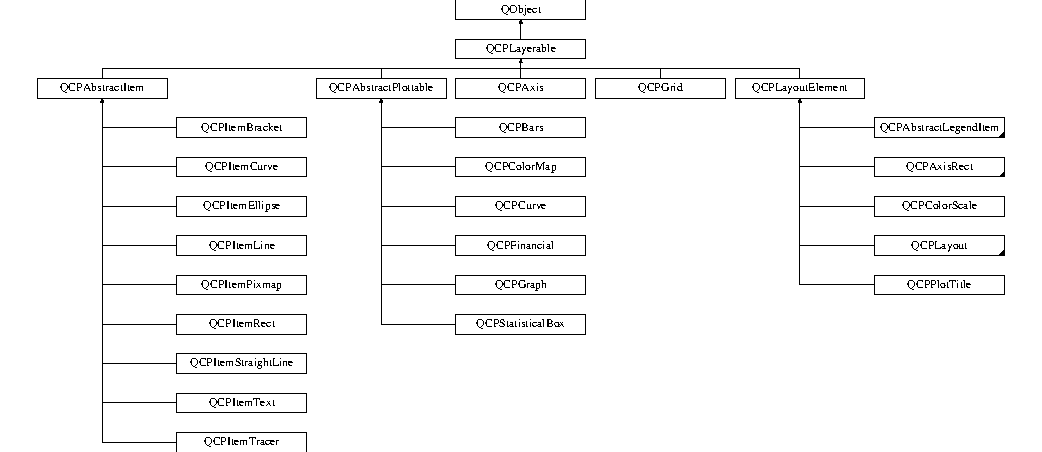
\includegraphics[height=6.075950cm]{class_q_c_p_layerable}
\end{center}
\end{figure}
\subsection*{Signals}
\begin{DoxyCompactItemize}
\item 
void \hyperlink{class_q_c_p_layerable_abbf8657cedea73ac1c3499b521c90eba}{layer\+Changed} (\hyperlink{class_q_c_p_layer}{Q\+C\+P\+Layer} $\ast$new\+Layer)
\end{DoxyCompactItemize}
\subsection*{Public Member Functions}
\begin{DoxyCompactItemize}
\item 
\hyperlink{class_q_c_p_layerable_a74c0fa237f29bf0e49565013fc5d1ec0}{Q\+C\+P\+Layerable} (\hyperlink{class_q_custom_plot}{Q\+Custom\+Plot} $\ast$plot, Q\+String target\+Layer=Q\+String(), \hyperlink{class_q_c_p_layerable}{Q\+C\+P\+Layerable} $\ast$\hyperlink{class_q_c_p_layerable_aa78b7e644d2c519e1a9a6f2ac5fcd858}{parent\+Layerable}=0)
\item 
\hypertarget{class_q_c_p_layerable_af0297b944b6192b6d67d00bff41b6b70}{}\label{class_q_c_p_layerable_af0297b944b6192b6d67d00bff41b6b70} 
bool {\bfseries visible} () const
\item 
\hypertarget{class_q_c_p_layerable_a473edb813a4c1929d6b6a8fe3ff3faf7}{}\label{class_q_c_p_layerable_a473edb813a4c1929d6b6a8fe3ff3faf7} 
\hyperlink{class_q_custom_plot}{Q\+Custom\+Plot} $\ast$ {\bfseries parent\+Plot} () const
\item 
\hyperlink{class_q_c_p_layerable}{Q\+C\+P\+Layerable} $\ast$ \hyperlink{class_q_c_p_layerable_aa78b7e644d2c519e1a9a6f2ac5fcd858}{parent\+Layerable} () const
\item 
\hypertarget{class_q_c_p_layerable_a5ff4862e8c784c9f5986dbc1533ba2a4}{}\label{class_q_c_p_layerable_a5ff4862e8c784c9f5986dbc1533ba2a4} 
\hyperlink{class_q_c_p_layer}{Q\+C\+P\+Layer} $\ast$ {\bfseries layer} () const
\item 
\hypertarget{class_q_c_p_layerable_a71cbd212fde2703cee076e204a475709}{}\label{class_q_c_p_layerable_a71cbd212fde2703cee076e204a475709} 
bool {\bfseries antialiased} () const
\item 
void \hyperlink{class_q_c_p_layerable_a3bed99ddc396b48ce3ebfdc0418744f8}{set\+Visible} (bool on)
\item 
Q\+\_\+\+S\+L\+OT bool \hyperlink{class_q_c_p_layerable_ab0d0da6d2de45a118886d2c8e16d5a54}{set\+Layer} (\hyperlink{class_q_c_p_layer}{Q\+C\+P\+Layer} $\ast$layer)
\item 
bool \hyperlink{class_q_c_p_layerable_ab25a0e7b897993b44447caee0f142083}{set\+Layer} (const Q\+String \&layer\+Name)
\item 
void \hyperlink{class_q_c_p_layerable_a4fd43e89be4a553ead41652565ff0581}{set\+Antialiased} (bool enabled)
\item 
virtual double \hyperlink{class_q_c_p_layerable_a04db8351fefd44cfdb77958e75c6288e}{select\+Test} (const Q\+PointF \&pos, bool only\+Selectable, Q\+Variant $\ast$details=0) const
\item 
bool \hyperlink{class_q_c_p_layerable_ab054e88f15d485defcb95e7376f119e7}{real\+Visibility} () const
\end{DoxyCompactItemize}
\subsection*{Protected Member Functions}
\begin{DoxyCompactItemize}
\item 
\hypertarget{class_q_c_p_layerable_ab20b7dbd8e0249ed61adb9622c427382}{}\label{class_q_c_p_layerable_ab20b7dbd8e0249ed61adb9622c427382} 
virtual void {\bfseries parent\+Plot\+Initialized} (\hyperlink{class_q_custom_plot}{Q\+Custom\+Plot} $\ast$parent\+Plot)
\item 
\hypertarget{class_q_c_p_layerable_a908c9edda761886f33893be326dab77d}{}\label{class_q_c_p_layerable_a908c9edda761886f33893be326dab77d} 
virtual \hyperlink{namespace_q_c_p_a2ad6bb6281c7c2d593d4277b44c2b037}{Q\+C\+P\+::\+Interaction} {\bfseries selection\+Category} () const
\item 
\hypertarget{class_q_c_p_layerable_acbcfc9ecc75433747b1978a77b1864b3}{}\label{class_q_c_p_layerable_acbcfc9ecc75433747b1978a77b1864b3} 
virtual Q\+Rect {\bfseries clip\+Rect} () const
\item 
\hypertarget{class_q_c_p_layerable_afdf83ddc6a265cbf4c89fe99d3d93473}{}\label{class_q_c_p_layerable_afdf83ddc6a265cbf4c89fe99d3d93473} 
virtual void {\bfseries apply\+Default\+Antialiasing\+Hint} (\hyperlink{class_q_c_p_painter}{Q\+C\+P\+Painter} $\ast$painter) const =0
\item 
\hypertarget{class_q_c_p_layerable_aecf2f7087482d4b6a78cb2770e5ed12d}{}\label{class_q_c_p_layerable_aecf2f7087482d4b6a78cb2770e5ed12d} 
virtual void {\bfseries draw} (\hyperlink{class_q_c_p_painter}{Q\+C\+P\+Painter} $\ast$painter)=0
\item 
\hypertarget{class_q_c_p_layerable_a7498c2d0d081cf7cad0fb3bb93aa0e91}{}\label{class_q_c_p_layerable_a7498c2d0d081cf7cad0fb3bb93aa0e91} 
virtual void {\bfseries select\+Event} (Q\+Mouse\+Event $\ast$event, bool additive, const Q\+Variant \&details, bool $\ast$selection\+State\+Changed)
\item 
\hypertarget{class_q_c_p_layerable_ae546370644a5551c76af739afc008bee}{}\label{class_q_c_p_layerable_ae546370644a5551c76af739afc008bee} 
virtual void {\bfseries deselect\+Event} (bool $\ast$selection\+State\+Changed)
\item 
\hypertarget{class_q_c_p_layerable_a8cbe5a0c9a5674249982f5ca5f8e02bc}{}\label{class_q_c_p_layerable_a8cbe5a0c9a5674249982f5ca5f8e02bc} 
void {\bfseries initialize\+Parent\+Plot} (\hyperlink{class_q_custom_plot}{Q\+Custom\+Plot} $\ast$parent\+Plot)
\item 
\hypertarget{class_q_c_p_layerable_aa23c893671f1f6744ac235cf2204cf3a}{}\label{class_q_c_p_layerable_aa23c893671f1f6744ac235cf2204cf3a} 
void {\bfseries set\+Parent\+Layerable} (\hyperlink{class_q_c_p_layerable}{Q\+C\+P\+Layerable} $\ast$\hyperlink{class_q_c_p_layerable_aa78b7e644d2c519e1a9a6f2ac5fcd858}{parent\+Layerable})
\item 
\hypertarget{class_q_c_p_layerable_af94484cfb7cbbddb7de522e9be71d9a4}{}\label{class_q_c_p_layerable_af94484cfb7cbbddb7de522e9be71d9a4} 
bool {\bfseries move\+To\+Layer} (\hyperlink{class_q_c_p_layer}{Q\+C\+P\+Layer} $\ast$layer, bool prepend)
\item 
\hypertarget{class_q_c_p_layerable_acb663e375d2d36dc5c55021ee5a2119b}{}\label{class_q_c_p_layerable_acb663e375d2d36dc5c55021ee5a2119b} 
void {\bfseries apply\+Antialiasing\+Hint} (\hyperlink{class_q_c_p_painter}{Q\+C\+P\+Painter} $\ast$painter, bool local\+Antialiased, \hyperlink{namespace_q_c_p_ae55dbe315d41fe80f29ba88100843a0c}{Q\+C\+P\+::\+Antialiased\+Element} override\+Element) const
\end{DoxyCompactItemize}
\subsection*{Protected Attributes}
\begin{DoxyCompactItemize}
\item 
\hypertarget{class_q_c_p_layerable_a62e3aed8427d6ce3ccf716f285106cb3}{}\label{class_q_c_p_layerable_a62e3aed8427d6ce3ccf716f285106cb3} 
bool {\bfseries m\+Visible}
\item 
\hypertarget{class_q_c_p_layerable_aa2a528433e44db02b8aef23c1f9f90ed}{}\label{class_q_c_p_layerable_aa2a528433e44db02b8aef23c1f9f90ed} 
\hyperlink{class_q_custom_plot}{Q\+Custom\+Plot} $\ast$ {\bfseries m\+Parent\+Plot}
\item 
\hypertarget{class_q_c_p_layerable_a3291445a980053e2d17a21d15957624e}{}\label{class_q_c_p_layerable_a3291445a980053e2d17a21d15957624e} 
Q\+Pointer$<$ \hyperlink{class_q_c_p_layerable}{Q\+C\+P\+Layerable} $>$ {\bfseries m\+Parent\+Layerable}
\item 
\hypertarget{class_q_c_p_layerable_aa38ec5891aff0f50b36fd63e9372a0cd}{}\label{class_q_c_p_layerable_aa38ec5891aff0f50b36fd63e9372a0cd} 
\hyperlink{class_q_c_p_layer}{Q\+C\+P\+Layer} $\ast$ {\bfseries m\+Layer}
\item 
\hypertarget{class_q_c_p_layerable_a3ab45a4c76a3333ce42eb217a81733ec}{}\label{class_q_c_p_layerable_a3ab45a4c76a3333ce42eb217a81733ec} 
bool {\bfseries m\+Antialiased}
\end{DoxyCompactItemize}
\subsection*{Friends}
\begin{DoxyCompactItemize}
\item 
\hypertarget{class_q_c_p_layerable_a1cdf9df76adcfae45261690aa0ca2198}{}\label{class_q_c_p_layerable_a1cdf9df76adcfae45261690aa0ca2198} 
class {\bfseries Q\+Custom\+Plot}
\item 
\hypertarget{class_q_c_p_layerable_acbf20ecb140f66c5fd1bc64ae0762990}{}\label{class_q_c_p_layerable_acbf20ecb140f66c5fd1bc64ae0762990} 
class {\bfseries Q\+C\+P\+Axis\+Rect}
\end{DoxyCompactItemize}


\subsection{Detailed Description}
Base class for all drawable objects. 

This is the abstract base class most visible objects derive from, e.\+g. plottables, axes, grid etc.

Every layerable is on a layer (\hyperlink{class_q_c_p_layer}{Q\+C\+P\+Layer}) which allows controlling the rendering order by stacking the layers accordingly.

For details about the layering mechanism, see the \hyperlink{class_q_c_p_layer}{Q\+C\+P\+Layer} documentation. 

\subsection{Constructor \& Destructor Documentation}
\hypertarget{class_q_c_p_layerable_a74c0fa237f29bf0e49565013fc5d1ec0}{}\label{class_q_c_p_layerable_a74c0fa237f29bf0e49565013fc5d1ec0} 
\index{Q\+C\+P\+Layerable@{Q\+C\+P\+Layerable}!Q\+C\+P\+Layerable@{Q\+C\+P\+Layerable}}
\index{Q\+C\+P\+Layerable@{Q\+C\+P\+Layerable}!Q\+C\+P\+Layerable@{Q\+C\+P\+Layerable}}
\subsubsection{\texorpdfstring{Q\+C\+P\+Layerable()}{QCPLayerable()}}
{\footnotesize\ttfamily Q\+C\+P\+Layerable\+::\+Q\+C\+P\+Layerable (\begin{DoxyParamCaption}\item[{\hyperlink{class_q_custom_plot}{Q\+Custom\+Plot} $\ast$}]{plot,  }\item[{Q\+String}]{target\+Layer = {\ttfamily QString()},  }\item[{\hyperlink{class_q_c_p_layerable}{Q\+C\+P\+Layerable} $\ast$}]{parent\+Layerable = {\ttfamily 0} }\end{DoxyParamCaption})}

Creates a new \hyperlink{class_q_c_p_layerable}{Q\+C\+P\+Layerable} instance.

Since \hyperlink{class_q_c_p_layerable}{Q\+C\+P\+Layerable} is an abstract base class, it can\textquotesingle{}t be instantiated directly. Use one of the derived classes.

If {\itshape plot} is provided, it automatically places itself on the layer named {\itshape target\+Layer}. If {\itshape target\+Layer} is an empty string, it places itself on the current layer of the plot (see \hyperlink{class_q_custom_plot_a73a6dc47c653bb6f8f030abca5a11852}{Q\+Custom\+Plot\+::set\+Current\+Layer}).

It is possible to provide 0 as {\itshape plot}. In that case, you should assign a parent plot at a later time with initialize\+Parent\+Plot.

The layerable\textquotesingle{}s parent layerable is set to {\itshape parent\+Layerable}, if provided. Direct layerable parents are mainly used to control visibility in a hierarchy of layerables. This means a layerable is only drawn, if all its ancestor layerables are also visible. Note that {\itshape parent\+Layerable} does not become the Q\+Object-\/parent (for memory management) of this layerable, {\itshape plot} does. It is not uncommon to set the Q\+Object-\/parent to something else in the constructors of \hyperlink{class_q_c_p_layerable}{Q\+C\+P\+Layerable} subclasses, to guarantee a working destruction hierarchy. 

\subsection{Member Function Documentation}
\hypertarget{class_q_c_p_layerable_abbf8657cedea73ac1c3499b521c90eba}{}\label{class_q_c_p_layerable_abbf8657cedea73ac1c3499b521c90eba} 
\index{Q\+C\+P\+Layerable@{Q\+C\+P\+Layerable}!layer\+Changed@{layer\+Changed}}
\index{layer\+Changed@{layer\+Changed}!Q\+C\+P\+Layerable@{Q\+C\+P\+Layerable}}
\subsubsection{\texorpdfstring{layer\+Changed}{layerChanged}}
{\footnotesize\ttfamily void Q\+C\+P\+Layerable\+::layer\+Changed (\begin{DoxyParamCaption}\item[{\hyperlink{class_q_c_p_layer}{Q\+C\+P\+Layer} $\ast$}]{new\+Layer }\end{DoxyParamCaption})\hspace{0.3cm}{\ttfamily [signal]}}

This signal is emitted when the layer of this layerable changes, i.\+e. this layerable is moved to a different layer.

\begin{DoxySeeAlso}{See also}
\hyperlink{class_q_c_p_layerable_ab0d0da6d2de45a118886d2c8e16d5a54}{set\+Layer} 
\end{DoxySeeAlso}
\hypertarget{class_q_c_p_layerable_aa78b7e644d2c519e1a9a6f2ac5fcd858}{}\label{class_q_c_p_layerable_aa78b7e644d2c519e1a9a6f2ac5fcd858} 
\index{Q\+C\+P\+Layerable@{Q\+C\+P\+Layerable}!parent\+Layerable@{parent\+Layerable}}
\index{parent\+Layerable@{parent\+Layerable}!Q\+C\+P\+Layerable@{Q\+C\+P\+Layerable}}
\subsubsection{\texorpdfstring{parent\+Layerable()}{parentLayerable()}}
{\footnotesize\ttfamily \hyperlink{class_q_c_p_layerable}{Q\+C\+P\+Layerable} $\ast$ Q\+C\+P\+Layerable\+::parent\+Layerable (\begin{DoxyParamCaption}{ }\end{DoxyParamCaption}) const\hspace{0.3cm}{\ttfamily [inline]}}

Returns the parent layerable of this layerable. The parent layerable is used to provide visibility hierarchies in conjunction with the method \hyperlink{class_q_c_p_layerable_ab054e88f15d485defcb95e7376f119e7}{real\+Visibility}. This way, layerables only get drawn if their parent layerables are visible, too.

Note that a parent layerable is not necessarily also the Q\+Object parent for memory management. Further, a layerable doesn\textquotesingle{}t always have a parent layerable, so this function may return 0.

A parent layerable is set implicitly with when placed inside layout elements and doesn\textquotesingle{}t need to be set manually by the user. \hypertarget{class_q_c_p_layerable_ab054e88f15d485defcb95e7376f119e7}{}\label{class_q_c_p_layerable_ab054e88f15d485defcb95e7376f119e7} 
\index{Q\+C\+P\+Layerable@{Q\+C\+P\+Layerable}!real\+Visibility@{real\+Visibility}}
\index{real\+Visibility@{real\+Visibility}!Q\+C\+P\+Layerable@{Q\+C\+P\+Layerable}}
\subsubsection{\texorpdfstring{real\+Visibility()}{realVisibility()}}
{\footnotesize\ttfamily bool Q\+C\+P\+Layerable\+::real\+Visibility (\begin{DoxyParamCaption}{ }\end{DoxyParamCaption}) const}

Returns whether this layerable is visible, taking the visibility of the layerable parent and the visibility of the layer this layerable is on into account. This is the method that is consulted to decide whether a layerable shall be drawn or not.

If this layerable has a direct layerable parent (usually set via hierarchies implemented in subclasses, like in the case of \hyperlink{class_q_c_p_layout_element}{Q\+C\+P\+Layout\+Element}), this function returns true only if this layerable has its visibility set to true and the parent layerable\textquotesingle{}s \hyperlink{class_q_c_p_layerable_ab054e88f15d485defcb95e7376f119e7}{real\+Visibility} returns true.

If this layerable doesn\textquotesingle{}t have a direct layerable parent, returns the state of this layerable\textquotesingle{}s visibility. \hypertarget{class_q_c_p_layerable_a04db8351fefd44cfdb77958e75c6288e}{}\label{class_q_c_p_layerable_a04db8351fefd44cfdb77958e75c6288e} 
\index{Q\+C\+P\+Layerable@{Q\+C\+P\+Layerable}!select\+Test@{select\+Test}}
\index{select\+Test@{select\+Test}!Q\+C\+P\+Layerable@{Q\+C\+P\+Layerable}}
\subsubsection{\texorpdfstring{select\+Test()}{selectTest()}}
{\footnotesize\ttfamily double Q\+C\+P\+Layerable\+::select\+Test (\begin{DoxyParamCaption}\item[{const Q\+PointF \&}]{pos,  }\item[{bool}]{only\+Selectable,  }\item[{Q\+Variant $\ast$}]{details = {\ttfamily 0} }\end{DoxyParamCaption}) const\hspace{0.3cm}{\ttfamily [virtual]}}

This function is used to decide whether a click hits a layerable object or not.

{\itshape pos} is a point in pixel coordinates on the \hyperlink{class_q_custom_plot}{Q\+Custom\+Plot} surface. This function returns the shortest pixel distance of this point to the object. If the object is either invisible or the distance couldn\textquotesingle{}t be determined, -\/1.\+0 is returned. Further, if {\itshape only\+Selectable} is true and the object is not selectable, -\/1.\+0 is returned, too.

If the object is represented not by single lines but by an area like a \hyperlink{class_q_c_p_item_text}{Q\+C\+P\+Item\+Text} or the bars of a \hyperlink{class_q_c_p_bars}{Q\+C\+P\+Bars} plottable, a click inside the area should also be considered a hit. In these cases this function thus returns a constant value greater zero but still below the parent plot\textquotesingle{}s selection tolerance. (typically the selection\+Tolerance multiplied by 0.\+99).

Providing a constant value for area objects allows selecting line objects even when they are obscured by such area objects, by clicking close to the lines (i.\+e. closer than 0.\+99$\ast$selection\+Tolerance).

The actual setting of the selection state is not done by this function. This is handled by the parent \hyperlink{class_q_custom_plot}{Q\+Custom\+Plot} when the mouse\+Release\+Event occurs, and the finally selected object is notified via the select\+Event/deselect\+Event methods.

{\itshape details} is an optional output parameter. Every layerable subclass may place any information in {\itshape details}. This information will be passed to select\+Event when the parent \hyperlink{class_q_custom_plot}{Q\+Custom\+Plot} decides on the basis of this select\+Test call, that the object was successfully selected. The subsequent call to select\+Event will carry the {\itshape details}. This is useful for multi-\/part objects (like \hyperlink{class_q_c_p_axis}{Q\+C\+P\+Axis}). This way, a possibly complex calculation to decide which part was clicked is only done once in \hyperlink{class_q_c_p_layerable_a04db8351fefd44cfdb77958e75c6288e}{select\+Test}. The result (i.\+e. the actually clicked part) can then be placed in {\itshape details}. So in the subsequent select\+Event, the decision which part was selected doesn\textquotesingle{}t have to be done a second time for a single selection operation.

You may pass 0 as {\itshape details} to indicate that you are not interested in those selection details.

\begin{DoxySeeAlso}{See also}
select\+Event, deselect\+Event, \hyperlink{class_q_custom_plot_a5ee1e2f6ae27419deca53e75907c27e5}{Q\+Custom\+Plot\+::set\+Interactions} 
\end{DoxySeeAlso}


Reimplemented in \hyperlink{class_q_c_p_item_bracket_a971299aa6fef75730d6f10efdaf48616}{Q\+C\+P\+Item\+Bracket}, \hyperlink{class_q_c_p_item_tracer_ae1dc728384936184e7552a6d0d67fd75}{Q\+C\+P\+Item\+Tracer}, \hyperlink{class_q_c_p_item_pixmap_a7583a98ebd3f35d2ac5d6c05fad25a6c}{Q\+C\+P\+Item\+Pixmap}, \hyperlink{class_q_c_p_item_ellipse_aa41be2180b2ace2e303b88d005c14243}{Q\+C\+P\+Item\+Ellipse}, \hyperlink{class_q_c_p_item_text_aca74494fd5e769f331a6eb3e29f32916}{Q\+C\+P\+Item\+Text}, \hyperlink{class_q_c_p_item_rect_abe1a6091591d3bad5e4efab2331f99ec}{Q\+C\+P\+Item\+Rect}, \hyperlink{class_q_c_p_item_curve_a8018b8b3fc552a44ba87ca4b64c1523f}{Q\+C\+P\+Item\+Curve}, \hyperlink{class_q_c_p_item_line_ae6cc5183f568e5fa9d7827abe4d405b5}{Q\+C\+P\+Item\+Line}, \hyperlink{class_q_c_p_item_straight_line_a1e5d99d79efb5871600c72bcd2891a0f}{Q\+C\+P\+Item\+Straight\+Line}, \hyperlink{class_q_c_p_financial_a77bffad8f3fcbcccbef03ead1c538e3a}{Q\+C\+P\+Financial}, \hyperlink{class_q_c_p_color_map_aba91ea58b489031157ecb777fe79e309}{Q\+C\+P\+Color\+Map}, \hyperlink{class_q_c_p_statistical_box_a0153ac16326b94450afbca208e3f9961}{Q\+C\+P\+Statistical\+Box}, \hyperlink{class_q_c_p_bars_a62d66cc8eedca6bedfc1f6513164d418}{Q\+C\+P\+Bars}, \hyperlink{class_q_c_p_curve_a87a9fb34a2a48dcae4c1245ada235e7d}{Q\+C\+P\+Curve}, \hyperlink{class_q_c_p_graph_a36011c34aca4f7a477de25961e2f6c13}{Q\+C\+P\+Graph}, \hyperlink{class_q_c_p_plot_title_aae4bcb2401e6947ea0abd3c960488d35}{Q\+C\+P\+Plot\+Title}, \hyperlink{class_q_c_p_legend_acd7be544c81324e391cfa6be9c413c01}{Q\+C\+P\+Legend}, \hyperlink{class_q_c_p_abstract_legend_item_ac834bf9003c491e5064a31e2a7de418d}{Q\+C\+P\+Abstract\+Legend\+Item}, \hyperlink{class_q_c_p_abstract_item_a96d522d10ffc0413b9a366c6f7f0476b}{Q\+C\+P\+Abstract\+Item}, \hyperlink{class_q_c_p_abstract_plottable_a38efe9641d972992a3d44204bc80ec1d}{Q\+C\+P\+Abstract\+Plottable}, \hyperlink{class_q_c_p_axis_a48e4f1bafd1826ba2ad46b691205bb90}{Q\+C\+P\+Axis}, \hyperlink{class_q_c_p_layout_inset_afcd56d5d1b8853838cdc535f1904f68a}{Q\+C\+P\+Layout\+Inset}, and \hyperlink{class_q_c_p_layout_element_a0b96ae0d7bcfa6e38188fcb1e73e143f}{Q\+C\+P\+Layout\+Element}.

\hypertarget{class_q_c_p_layerable_a4fd43e89be4a553ead41652565ff0581}{}\label{class_q_c_p_layerable_a4fd43e89be4a553ead41652565ff0581} 
\index{Q\+C\+P\+Layerable@{Q\+C\+P\+Layerable}!set\+Antialiased@{set\+Antialiased}}
\index{set\+Antialiased@{set\+Antialiased}!Q\+C\+P\+Layerable@{Q\+C\+P\+Layerable}}
\subsubsection{\texorpdfstring{set\+Antialiased()}{setAntialiased()}}
{\footnotesize\ttfamily void Q\+C\+P\+Layerable\+::set\+Antialiased (\begin{DoxyParamCaption}\item[{bool}]{enabled }\end{DoxyParamCaption})}

Sets whether this object will be drawn antialiased or not.

Note that antialiasing settings may be overridden by \hyperlink{class_q_custom_plot_af6f91e5eab1be85f67c556e98c3745e8}{Q\+Custom\+Plot\+::set\+Antialiased\+Elements} and \hyperlink{class_q_custom_plot_ae10d685b5eabea2999fb8775ca173c24}{Q\+Custom\+Plot\+::set\+Not\+Antialiased\+Elements}. \hypertarget{class_q_c_p_layerable_ab0d0da6d2de45a118886d2c8e16d5a54}{}\label{class_q_c_p_layerable_ab0d0da6d2de45a118886d2c8e16d5a54} 
\index{Q\+C\+P\+Layerable@{Q\+C\+P\+Layerable}!set\+Layer@{set\+Layer}}
\index{set\+Layer@{set\+Layer}!Q\+C\+P\+Layerable@{Q\+C\+P\+Layerable}}
\subsubsection{\texorpdfstring{set\+Layer()}{setLayer()}\hspace{0.1cm}{\footnotesize\ttfamily [1/2]}}
{\footnotesize\ttfamily bool Q\+C\+P\+Layerable\+::set\+Layer (\begin{DoxyParamCaption}\item[{\hyperlink{class_q_c_p_layer}{Q\+C\+P\+Layer} $\ast$}]{layer }\end{DoxyParamCaption})}

Sets the {\itshape layer} of this layerable object. The object will be placed on top of the other objects already on {\itshape layer}.

If {\itshape layer} is 0, this layerable will not be on any layer and thus not appear in the plot (or interact/receive events).

Returns true if the layer of this layerable was successfully changed to {\itshape layer}. \hypertarget{class_q_c_p_layerable_ab25a0e7b897993b44447caee0f142083}{}\label{class_q_c_p_layerable_ab25a0e7b897993b44447caee0f142083} 
\index{Q\+C\+P\+Layerable@{Q\+C\+P\+Layerable}!set\+Layer@{set\+Layer}}
\index{set\+Layer@{set\+Layer}!Q\+C\+P\+Layerable@{Q\+C\+P\+Layerable}}
\subsubsection{\texorpdfstring{set\+Layer()}{setLayer()}\hspace{0.1cm}{\footnotesize\ttfamily [2/2]}}
{\footnotesize\ttfamily bool Q\+C\+P\+Layerable\+::set\+Layer (\begin{DoxyParamCaption}\item[{const Q\+String \&}]{layer\+Name }\end{DoxyParamCaption})}

This is an overloaded member function, provided for convenience. It differs from the above function only in what argument(s) it accepts. Sets the layer of this layerable object by name

Returns true on success, i.\+e. if {\itshape layer\+Name} is a valid layer name. \hypertarget{class_q_c_p_layerable_a3bed99ddc396b48ce3ebfdc0418744f8}{}\label{class_q_c_p_layerable_a3bed99ddc396b48ce3ebfdc0418744f8} 
\index{Q\+C\+P\+Layerable@{Q\+C\+P\+Layerable}!set\+Visible@{set\+Visible}}
\index{set\+Visible@{set\+Visible}!Q\+C\+P\+Layerable@{Q\+C\+P\+Layerable}}
\subsubsection{\texorpdfstring{set\+Visible()}{setVisible()}}
{\footnotesize\ttfamily void Q\+C\+P\+Layerable\+::set\+Visible (\begin{DoxyParamCaption}\item[{bool}]{on }\end{DoxyParamCaption})}

Sets the visibility of this layerable object. If an object is not visible, it will not be drawn on the \hyperlink{class_q_custom_plot}{Q\+Custom\+Plot} surface, and user interaction with it (e.\+g. click and selection) is not possible. 

The documentation for this class was generated from the following files\+:\begin{DoxyCompactItemize}
\item 
F\+E\+S\+S-\/\+G\+U\+I/\hyperlink{qcustomplot_8h}{qcustomplot.\+h}\item 
F\+E\+S\+S-\/\+G\+U\+I/\hyperlink{qcustomplot_8cpp}{qcustomplot.\+cpp}\end{DoxyCompactItemize}

\hypertarget{class_q_c_p_layout}{}\section{Q\+C\+P\+Layout Class Reference}
\label{class_q_c_p_layout}\index{Q\+C\+P\+Layout@{Q\+C\+P\+Layout}}


The abstract base class for layouts.  


Inheritance diagram for Q\+C\+P\+Layout\+:\begin{figure}[H]
\begin{center}
\leavevmode
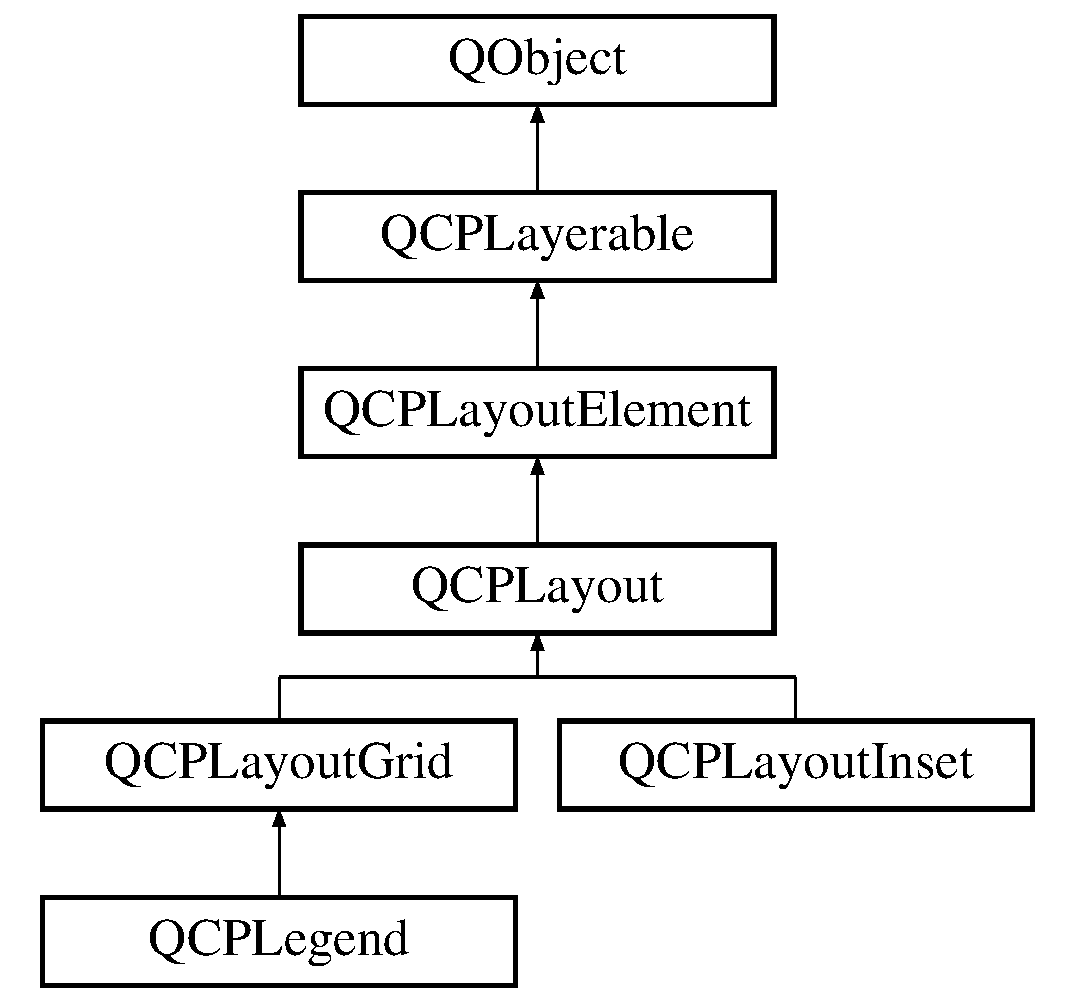
\includegraphics[height=6.000000cm]{class_q_c_p_layout}
\end{center}
\end{figure}
\subsection*{Public Member Functions}
\begin{DoxyCompactItemize}
\item 
\hyperlink{class_q_c_p_layout_a04222e6e1361fd802d48f1a25b7020d4}{Q\+C\+P\+Layout} ()
\item 
virtual void \hyperlink{class_q_c_p_layout_a34ab477e820537ded7bade4399c482fd}{update} (\hyperlink{class_q_c_p_layout_element_a0d83360e05735735aaf6d7983c56374d}{Update\+Phase} phase)
\item 
virtual Q\+List$<$ \hyperlink{class_q_c_p_layout_element}{Q\+C\+P\+Layout\+Element} $\ast$ $>$ \hyperlink{class_q_c_p_layout_adc9ebc73fc215f9cc22796712a251ff4}{elements} (bool recursive) const
\item 
virtual int \hyperlink{class_q_c_p_layout_a39d3e9ef5d9b82ab1885ba1cb9597e56}{element\+Count} () const =0
\item 
virtual \hyperlink{class_q_c_p_layout_element}{Q\+C\+P\+Layout\+Element} $\ast$ \hyperlink{class_q_c_p_layout_afa73ca7d859f8a3ee5c73c9b353d2a56}{element\+At} (int index) const =0
\item 
virtual \hyperlink{class_q_c_p_layout_element}{Q\+C\+P\+Layout\+Element} $\ast$ \hyperlink{class_q_c_p_layout_a5a79621fa0a6eabb8b520cfc04fb601a}{take\+At} (int index)=0
\item 
virtual bool \hyperlink{class_q_c_p_layout_ada26cd17e56472b0b4d7fbbc96873e4c}{take} (\hyperlink{class_q_c_p_layout_element}{Q\+C\+P\+Layout\+Element} $\ast$element)=0
\item 
virtual void \hyperlink{class_q_c_p_layout_a41e6ac049143866e8f8b4964efab01b2}{simplify} ()
\item 
bool \hyperlink{class_q_c_p_layout_a2403f684fee3ce47132faaeed00bb066}{remove\+At} (int index)
\item 
bool \hyperlink{class_q_c_p_layout_a6c58f537d8086f352576ab7c5b15d0bc}{remove} (\hyperlink{class_q_c_p_layout_element}{Q\+C\+P\+Layout\+Element} $\ast$element)
\item 
void \hyperlink{class_q_c_p_layout_a02883bdf2769b5b227f0232dba1ac4ee}{clear} ()
\end{DoxyCompactItemize}
\subsection*{Protected Member Functions}
\begin{DoxyCompactItemize}
\item 
\hypertarget{class_q_c_p_layout_a165c77f6287ac92e8d03017ad913378b}{}\label{class_q_c_p_layout_a165c77f6287ac92e8d03017ad913378b} 
virtual void {\bfseries update\+Layout} ()
\item 
void \hyperlink{class_q_c_p_layout_aeac66a292f65cf7f8adf94eb92345b3e}{size\+Constraints\+Changed} () const
\item 
\hypertarget{class_q_c_p_layout_af6dbbc24156a808da29cd1ec031729a3}{}\label{class_q_c_p_layout_af6dbbc24156a808da29cd1ec031729a3} 
void {\bfseries adopt\+Element} (\hyperlink{class_q_c_p_layout_element}{Q\+C\+P\+Layout\+Element} $\ast$el)
\item 
\hypertarget{class_q_c_p_layout_a4afbb4bef0071f72f91afdac4433a18e}{}\label{class_q_c_p_layout_a4afbb4bef0071f72f91afdac4433a18e} 
void {\bfseries release\+Element} (\hyperlink{class_q_c_p_layout_element}{Q\+C\+P\+Layout\+Element} $\ast$el)
\item 
\hypertarget{class_q_c_p_layout_a3e77be8006d39f2aafc1313d6e8fc3fd}{}\label{class_q_c_p_layout_a3e77be8006d39f2aafc1313d6e8fc3fd} 
Q\+Vector$<$ int $>$ {\bfseries get\+Section\+Sizes} (Q\+Vector$<$ int $>$ max\+Sizes, Q\+Vector$<$ int $>$ min\+Sizes, Q\+Vector$<$ double $>$ stretch\+Factors, int total\+Size) const
\end{DoxyCompactItemize}
\subsection*{Friends}
\begin{DoxyCompactItemize}
\item 
\hypertarget{class_q_c_p_layout_a0790750c7e7f14fdbd960d172655b42b}{}\label{class_q_c_p_layout_a0790750c7e7f14fdbd960d172655b42b} 
class {\bfseries Q\+C\+P\+Layout\+Element}
\end{DoxyCompactItemize}
\subsection*{Additional Inherited Members}


\subsection{Detailed Description}
The abstract base class for layouts. 

This is an abstract base class for layout elements whose main purpose is to define the position and size of other child layout elements. In most cases, layouts don\textquotesingle{}t draw anything themselves (but there are exceptions to this, e.\+g. \hyperlink{class_q_c_p_legend}{Q\+C\+P\+Legend}).

\hyperlink{class_q_c_p_layout}{Q\+C\+P\+Layout} derives from \hyperlink{class_q_c_p_layout_element}{Q\+C\+P\+Layout\+Element}, and thus can itself be nested in other layouts.

\hyperlink{class_q_c_p_layout}{Q\+C\+P\+Layout} introduces a common interface for accessing and manipulating the child elements. Those functions are most notably \hyperlink{class_q_c_p_layout_a39d3e9ef5d9b82ab1885ba1cb9597e56}{element\+Count}, \hyperlink{class_q_c_p_layout_afa73ca7d859f8a3ee5c73c9b353d2a56}{element\+At}, \hyperlink{class_q_c_p_layout_a5a79621fa0a6eabb8b520cfc04fb601a}{take\+At}, \hyperlink{class_q_c_p_layout_ada26cd17e56472b0b4d7fbbc96873e4c}{take}, \hyperlink{class_q_c_p_layout_a41e6ac049143866e8f8b4964efab01b2}{simplify}, \hyperlink{class_q_c_p_layout_a2403f684fee3ce47132faaeed00bb066}{remove\+At}, \hyperlink{class_q_c_p_layout_a6c58f537d8086f352576ab7c5b15d0bc}{remove} and \hyperlink{class_q_c_p_layout_a02883bdf2769b5b227f0232dba1ac4ee}{clear}. Individual subclasses may add more functions to this interface which are more specialized to the form of the layout. For example, \hyperlink{class_q_c_p_layout_grid}{Q\+C\+P\+Layout\+Grid} adds functions that take row and column indices to access cells of the layout grid more conveniently.

Since this is an abstract base class, you can\textquotesingle{}t instantiate it directly. Rather use one of its subclasses like \hyperlink{class_q_c_p_layout_grid}{Q\+C\+P\+Layout\+Grid} or \hyperlink{class_q_c_p_layout_inset}{Q\+C\+P\+Layout\+Inset}.

For a general introduction to the layout system, see the dedicated documentation page The Layout System. 

\subsection{Constructor \& Destructor Documentation}
\hypertarget{class_q_c_p_layout_a04222e6e1361fd802d48f1a25b7020d4}{}\label{class_q_c_p_layout_a04222e6e1361fd802d48f1a25b7020d4} 
\index{Q\+C\+P\+Layout@{Q\+C\+P\+Layout}!Q\+C\+P\+Layout@{Q\+C\+P\+Layout}}
\index{Q\+C\+P\+Layout@{Q\+C\+P\+Layout}!Q\+C\+P\+Layout@{Q\+C\+P\+Layout}}
\subsubsection{\texorpdfstring{Q\+C\+P\+Layout()}{QCPLayout()}}
{\footnotesize\ttfamily Q\+C\+P\+Layout\+::\+Q\+C\+P\+Layout (\begin{DoxyParamCaption}{ }\end{DoxyParamCaption})\hspace{0.3cm}{\ttfamily [explicit]}}

Creates an instance of \hyperlink{class_q_c_p_layout}{Q\+C\+P\+Layout} and sets default values. Note that since \hyperlink{class_q_c_p_layout}{Q\+C\+P\+Layout} is an abstract base class, it can\textquotesingle{}t be instantiated directly. 

\subsection{Member Function Documentation}
\hypertarget{class_q_c_p_layout_a02883bdf2769b5b227f0232dba1ac4ee}{}\label{class_q_c_p_layout_a02883bdf2769b5b227f0232dba1ac4ee} 
\index{Q\+C\+P\+Layout@{Q\+C\+P\+Layout}!clear@{clear}}
\index{clear@{clear}!Q\+C\+P\+Layout@{Q\+C\+P\+Layout}}
\subsubsection{\texorpdfstring{clear()}{clear()}}
{\footnotesize\ttfamily void Q\+C\+P\+Layout\+::clear (\begin{DoxyParamCaption}{ }\end{DoxyParamCaption})}

Removes and deletes all layout elements in this layout. Finally calls \hyperlink{class_q_c_p_layout_a41e6ac049143866e8f8b4964efab01b2}{simplify} to make sure all empty cells are collapsed.

\begin{DoxySeeAlso}{See also}
\hyperlink{class_q_c_p_layout_a6c58f537d8086f352576ab7c5b15d0bc}{remove}, \hyperlink{class_q_c_p_layout_a2403f684fee3ce47132faaeed00bb066}{remove\+At} 
\end{DoxySeeAlso}
\hypertarget{class_q_c_p_layout_afa73ca7d859f8a3ee5c73c9b353d2a56}{}\label{class_q_c_p_layout_afa73ca7d859f8a3ee5c73c9b353d2a56} 
\index{Q\+C\+P\+Layout@{Q\+C\+P\+Layout}!element\+At@{element\+At}}
\index{element\+At@{element\+At}!Q\+C\+P\+Layout@{Q\+C\+P\+Layout}}
\subsubsection{\texorpdfstring{element\+At()}{elementAt()}}
{\footnotesize\ttfamily \hyperlink{class_q_c_p_layout_element}{Q\+C\+P\+Layout\+Element} $\ast$ Q\+C\+P\+Layout\+::element\+At (\begin{DoxyParamCaption}\item[{int}]{index }\end{DoxyParamCaption}) const\hspace{0.3cm}{\ttfamily [pure virtual]}}

Returns the element in the cell with the given {\itshape index}. If {\itshape index} is invalid, returns 0.

Note that even if {\itshape index} is valid, the respective cell may be empty in some layouts (e.\+g. \hyperlink{class_q_c_p_layout_grid}{Q\+C\+P\+Layout\+Grid}), so this function may return 0 in those cases. You may use this function to check whether a cell is empty or not.

\begin{DoxySeeAlso}{See also}
\hyperlink{class_q_c_p_layout_adc9ebc73fc215f9cc22796712a251ff4}{elements}, \hyperlink{class_q_c_p_layout_a39d3e9ef5d9b82ab1885ba1cb9597e56}{element\+Count}, \hyperlink{class_q_c_p_layout_a5a79621fa0a6eabb8b520cfc04fb601a}{take\+At} 
\end{DoxySeeAlso}


Implemented in \hyperlink{class_q_c_p_layout_inset_a832e049f0bb32e7db0490a9c904098df}{Q\+C\+P\+Layout\+Inset}, and \hyperlink{class_q_c_p_layout_grid_a97672ecc379cb3a09639926ba9980297}{Q\+C\+P\+Layout\+Grid}.

\hypertarget{class_q_c_p_layout_a39d3e9ef5d9b82ab1885ba1cb9597e56}{}\label{class_q_c_p_layout_a39d3e9ef5d9b82ab1885ba1cb9597e56} 
\index{Q\+C\+P\+Layout@{Q\+C\+P\+Layout}!element\+Count@{element\+Count}}
\index{element\+Count@{element\+Count}!Q\+C\+P\+Layout@{Q\+C\+P\+Layout}}
\subsubsection{\texorpdfstring{element\+Count()}{elementCount()}}
{\footnotesize\ttfamily int Q\+C\+P\+Layout\+::element\+Count (\begin{DoxyParamCaption}{ }\end{DoxyParamCaption}) const\hspace{0.3cm}{\ttfamily [pure virtual]}}

Returns the number of elements/cells in the layout.

\begin{DoxySeeAlso}{See also}
\hyperlink{class_q_c_p_layout_adc9ebc73fc215f9cc22796712a251ff4}{elements}, \hyperlink{class_q_c_p_layout_afa73ca7d859f8a3ee5c73c9b353d2a56}{element\+At} 
\end{DoxySeeAlso}


Implemented in \hyperlink{class_q_c_p_layout_inset_a0398918a888fa7974a6776dc47fc5d2e}{Q\+C\+P\+Layout\+Inset}, and \hyperlink{class_q_c_p_layout_grid_a77f194843d037e0da6d5f3170acdf3a2}{Q\+C\+P\+Layout\+Grid}.

\hypertarget{class_q_c_p_layout_adc9ebc73fc215f9cc22796712a251ff4}{}\label{class_q_c_p_layout_adc9ebc73fc215f9cc22796712a251ff4} 
\index{Q\+C\+P\+Layout@{Q\+C\+P\+Layout}!elements@{elements}}
\index{elements@{elements}!Q\+C\+P\+Layout@{Q\+C\+P\+Layout}}
\subsubsection{\texorpdfstring{elements()}{elements()}}
{\footnotesize\ttfamily Q\+List$<$ \hyperlink{class_q_c_p_layout_element}{Q\+C\+P\+Layout\+Element} $\ast$ $>$ Q\+C\+P\+Layout\+::elements (\begin{DoxyParamCaption}\item[{bool}]{recursive }\end{DoxyParamCaption}) const\hspace{0.3cm}{\ttfamily [virtual]}}

Returns a list of all child elements in this layout element. If {\itshape recursive} is true, all sub-\/child elements are included in the list, too.

\begin{DoxyWarning}{Warning}
There may be entries with value 0 in the returned list. (For example, \hyperlink{class_q_c_p_layout_grid}{Q\+C\+P\+Layout\+Grid} may have empty cells which yield 0 at the respective index.) 
\end{DoxyWarning}


Reimplemented from \hyperlink{class_q_c_p_layout_element_a76dec8cb31e498994a944d7647a43309}{Q\+C\+P\+Layout\+Element}.



Reimplemented in \hyperlink{class_q_c_p_layout_grid_a20a745d013de4c89cf5de8004a5a36f7}{Q\+C\+P\+Layout\+Grid}.

\hypertarget{class_q_c_p_layout_a6c58f537d8086f352576ab7c5b15d0bc}{}\label{class_q_c_p_layout_a6c58f537d8086f352576ab7c5b15d0bc} 
\index{Q\+C\+P\+Layout@{Q\+C\+P\+Layout}!remove@{remove}}
\index{remove@{remove}!Q\+C\+P\+Layout@{Q\+C\+P\+Layout}}
\subsubsection{\texorpdfstring{remove()}{remove()}}
{\footnotesize\ttfamily bool Q\+C\+P\+Layout\+::remove (\begin{DoxyParamCaption}\item[{\hyperlink{class_q_c_p_layout_element}{Q\+C\+P\+Layout\+Element} $\ast$}]{element }\end{DoxyParamCaption})}

Removes and deletes the provided {\itshape element}. Returns true on success. If {\itshape element} is not in the layout, returns false.

This function internally uses \hyperlink{class_q_c_p_layout_a5a79621fa0a6eabb8b520cfc04fb601a}{take\+At} to remove the element from the layout and then deletes the element. Note that some layouts don\textquotesingle{}t remove the respective cell right away but leave an empty cell after successful removal of the layout element. To collapse empty cells, use \hyperlink{class_q_c_p_layout_a41e6ac049143866e8f8b4964efab01b2}{simplify}.

\begin{DoxySeeAlso}{See also}
\hyperlink{class_q_c_p_layout_a2403f684fee3ce47132faaeed00bb066}{remove\+At}, \hyperlink{class_q_c_p_layout_ada26cd17e56472b0b4d7fbbc96873e4c}{take} 
\end{DoxySeeAlso}
\hypertarget{class_q_c_p_layout_a2403f684fee3ce47132faaeed00bb066}{}\label{class_q_c_p_layout_a2403f684fee3ce47132faaeed00bb066} 
\index{Q\+C\+P\+Layout@{Q\+C\+P\+Layout}!remove\+At@{remove\+At}}
\index{remove\+At@{remove\+At}!Q\+C\+P\+Layout@{Q\+C\+P\+Layout}}
\subsubsection{\texorpdfstring{remove\+At()}{removeAt()}}
{\footnotesize\ttfamily bool Q\+C\+P\+Layout\+::remove\+At (\begin{DoxyParamCaption}\item[{int}]{index }\end{DoxyParamCaption})}

Removes and deletes the element at the provided {\itshape index}. Returns true on success. If {\itshape index} is invalid or points to an empty cell, returns false.

This function internally uses \hyperlink{class_q_c_p_layout_a5a79621fa0a6eabb8b520cfc04fb601a}{take\+At} to remove the element from the layout and then deletes the returned element. Note that some layouts don\textquotesingle{}t remove the respective cell right away but leave an empty cell after successful removal of the layout element. To collapse empty cells, use \hyperlink{class_q_c_p_layout_a41e6ac049143866e8f8b4964efab01b2}{simplify}.

\begin{DoxySeeAlso}{See also}
\hyperlink{class_q_c_p_layout_a6c58f537d8086f352576ab7c5b15d0bc}{remove}, \hyperlink{class_q_c_p_layout_a5a79621fa0a6eabb8b520cfc04fb601a}{take\+At} 
\end{DoxySeeAlso}
\hypertarget{class_q_c_p_layout_a41e6ac049143866e8f8b4964efab01b2}{}\label{class_q_c_p_layout_a41e6ac049143866e8f8b4964efab01b2} 
\index{Q\+C\+P\+Layout@{Q\+C\+P\+Layout}!simplify@{simplify}}
\index{simplify@{simplify}!Q\+C\+P\+Layout@{Q\+C\+P\+Layout}}
\subsubsection{\texorpdfstring{simplify()}{simplify()}}
{\footnotesize\ttfamily void Q\+C\+P\+Layout\+::simplify (\begin{DoxyParamCaption}{ }\end{DoxyParamCaption})\hspace{0.3cm}{\ttfamily [virtual]}}

Simplifies the layout by collapsing empty cells. The exact behavior depends on subclasses, the default implementation does nothing.

Not all layouts need simplification. For example, \hyperlink{class_q_c_p_layout_inset}{Q\+C\+P\+Layout\+Inset} doesn\textquotesingle{}t use explicit simplification while \hyperlink{class_q_c_p_layout_grid}{Q\+C\+P\+Layout\+Grid} does. 

Reimplemented in \hyperlink{class_q_c_p_layout_inset_abb9eb23bf2d7c587a8abe02d065eae0a}{Q\+C\+P\+Layout\+Inset}, and \hyperlink{class_q_c_p_layout_grid_a08bba60e4acd20165526a8fd7f986b58}{Q\+C\+P\+Layout\+Grid}.

\hypertarget{class_q_c_p_layout_aeac66a292f65cf7f8adf94eb92345b3e}{}\label{class_q_c_p_layout_aeac66a292f65cf7f8adf94eb92345b3e} 
\index{Q\+C\+P\+Layout@{Q\+C\+P\+Layout}!size\+Constraints\+Changed@{size\+Constraints\+Changed}}
\index{size\+Constraints\+Changed@{size\+Constraints\+Changed}!Q\+C\+P\+Layout@{Q\+C\+P\+Layout}}
\subsubsection{\texorpdfstring{size\+Constraints\+Changed()}{sizeConstraintsChanged()}}
{\footnotesize\ttfamily void Q\+C\+P\+Layout\+::size\+Constraints\+Changed (\begin{DoxyParamCaption}{ }\end{DoxyParamCaption}) const\hspace{0.3cm}{\ttfamily [protected]}}

Subclasses call this method to report changed (minimum/maximum) size constraints.

If the parent of this layout is again a \hyperlink{class_q_c_p_layout}{Q\+C\+P\+Layout}, forwards the call to the parent\textquotesingle{}s \hyperlink{class_q_c_p_layout_aeac66a292f65cf7f8adf94eb92345b3e}{size\+Constraints\+Changed}. If the parent is a Q\+Widget (i.\+e. is the \hyperlink{class_q_custom_plot_af1a1f1f571237deb7c2bd34a5e9f018f}{Q\+Custom\+Plot\+::plot\+Layout} of \hyperlink{class_q_custom_plot}{Q\+Custom\+Plot}), calls Q\+Widget\+::update\+Geometry, so if the \hyperlink{class_q_custom_plot}{Q\+Custom\+Plot} widget is inside a Qt Q\+Layout, it may update itself and resize cells accordingly. \hypertarget{class_q_c_p_layout_ada26cd17e56472b0b4d7fbbc96873e4c}{}\label{class_q_c_p_layout_ada26cd17e56472b0b4d7fbbc96873e4c} 
\index{Q\+C\+P\+Layout@{Q\+C\+P\+Layout}!take@{take}}
\index{take@{take}!Q\+C\+P\+Layout@{Q\+C\+P\+Layout}}
\subsubsection{\texorpdfstring{take()}{take()}}
{\footnotesize\ttfamily bool Q\+C\+P\+Layout\+::take (\begin{DoxyParamCaption}\item[{\hyperlink{class_q_c_p_layout_element}{Q\+C\+P\+Layout\+Element} $\ast$}]{element }\end{DoxyParamCaption})\hspace{0.3cm}{\ttfamily [pure virtual]}}

Removes the specified {\itshape element} from the layout and returns true on success.

If the {\itshape element} isn\textquotesingle{}t in this layout, returns false.

Note that some layouts don\textquotesingle{}t remove the respective cell right away but leave an empty cell after successful removal of the layout element. To collapse empty cells, use \hyperlink{class_q_c_p_layout_a41e6ac049143866e8f8b4964efab01b2}{simplify}.

\begin{DoxySeeAlso}{See also}
\hyperlink{class_q_c_p_layout_a5a79621fa0a6eabb8b520cfc04fb601a}{take\+At} 
\end{DoxySeeAlso}


Implemented in \hyperlink{class_q_c_p_layout_inset_a9ac707ccff650633b97f52dd5cddcf49}{Q\+C\+P\+Layout\+Inset}, and \hyperlink{class_q_c_p_layout_grid_a666a9fe9e92054436f9b66eba25cca0c}{Q\+C\+P\+Layout\+Grid}.

\hypertarget{class_q_c_p_layout_a5a79621fa0a6eabb8b520cfc04fb601a}{}\label{class_q_c_p_layout_a5a79621fa0a6eabb8b520cfc04fb601a} 
\index{Q\+C\+P\+Layout@{Q\+C\+P\+Layout}!take\+At@{take\+At}}
\index{take\+At@{take\+At}!Q\+C\+P\+Layout@{Q\+C\+P\+Layout}}
\subsubsection{\texorpdfstring{take\+At()}{takeAt()}}
{\footnotesize\ttfamily \hyperlink{class_q_c_p_layout_element}{Q\+C\+P\+Layout\+Element} $\ast$ Q\+C\+P\+Layout\+::take\+At (\begin{DoxyParamCaption}\item[{int}]{index }\end{DoxyParamCaption})\hspace{0.3cm}{\ttfamily [pure virtual]}}

Removes the element with the given {\itshape index} from the layout and returns it.

If the {\itshape index} is invalid or the cell with that index is empty, returns 0.

Note that some layouts don\textquotesingle{}t remove the respective cell right away but leave an empty cell after successful removal of the layout element. To collapse empty cells, use \hyperlink{class_q_c_p_layout_a41e6ac049143866e8f8b4964efab01b2}{simplify}.

\begin{DoxySeeAlso}{See also}
\hyperlink{class_q_c_p_layout_afa73ca7d859f8a3ee5c73c9b353d2a56}{element\+At}, \hyperlink{class_q_c_p_layout_ada26cd17e56472b0b4d7fbbc96873e4c}{take} 
\end{DoxySeeAlso}


Implemented in \hyperlink{class_q_c_p_layout_inset_ad6756a3b507e20496aaf7f5ca16c47d1}{Q\+C\+P\+Layout\+Inset}, and \hyperlink{class_q_c_p_layout_grid_acc1277394ff8a6432e111ff9463e6375}{Q\+C\+P\+Layout\+Grid}.

\hypertarget{class_q_c_p_layout_a34ab477e820537ded7bade4399c482fd}{}\label{class_q_c_p_layout_a34ab477e820537ded7bade4399c482fd} 
\index{Q\+C\+P\+Layout@{Q\+C\+P\+Layout}!update@{update}}
\index{update@{update}!Q\+C\+P\+Layout@{Q\+C\+P\+Layout}}
\subsubsection{\texorpdfstring{update()}{update()}}
{\footnotesize\ttfamily void Q\+C\+P\+Layout\+::update (\begin{DoxyParamCaption}\item[{\hyperlink{class_q_c_p_layout_element_a0d83360e05735735aaf6d7983c56374d}{Update\+Phase}}]{phase }\end{DoxyParamCaption})\hspace{0.3cm}{\ttfamily [virtual]}}

First calls the \hyperlink{class_q_c_p_layout_element_a929c2ec62e0e0e1d8418eaa802e2af9b}{Q\+C\+P\+Layout\+Element\+::update} base class implementation to update the margins on this layout.

Then calls update\+Layout which subclasses reimplement to reposition and resize their cells.

Finally, \hyperlink{class_q_c_p_layout_a34ab477e820537ded7bade4399c482fd}{update} is called on all child elements. 

Reimplemented from \hyperlink{class_q_c_p_layout_element_a929c2ec62e0e0e1d8418eaa802e2af9b}{Q\+C\+P\+Layout\+Element}.



The documentation for this class was generated from the following files\+:\begin{DoxyCompactItemize}
\item 
F\+E\+S\+S-\/\+G\+U\+I/\hyperlink{qcustomplot_8h}{qcustomplot.\+h}\item 
F\+E\+S\+S-\/\+G\+U\+I/\hyperlink{qcustomplot_8cpp}{qcustomplot.\+cpp}\end{DoxyCompactItemize}

\hypertarget{class_q_c_p_layout_element}{}\section{Q\+C\+P\+Layout\+Element Class Reference}
\label{class_q_c_p_layout_element}\index{Q\+C\+P\+Layout\+Element@{Q\+C\+P\+Layout\+Element}}


The abstract base class for all objects that form the layout system.  


Inheritance diagram for Q\+C\+P\+Layout\+Element\+:\begin{figure}[H]
\begin{center}
\leavevmode
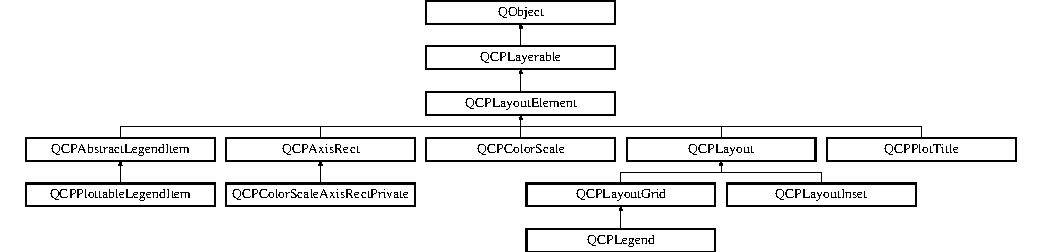
\includegraphics[height=3.376884cm]{class_q_c_p_layout_element}
\end{center}
\end{figure}
\subsection*{Public Types}
\begin{DoxyCompactItemize}
\item 
enum \hyperlink{class_q_c_p_layout_element_a0d83360e05735735aaf6d7983c56374d}{Update\+Phase} \{ \hyperlink{class_q_c_p_layout_element_a0d83360e05735735aaf6d7983c56374dad6119882eba136357c2f627992e527d3}{up\+Preparation}, 
\hyperlink{class_q_c_p_layout_element_a0d83360e05735735aaf6d7983c56374da288cb59a92280e47261a341f2813e676}{up\+Margins}, 
\hyperlink{class_q_c_p_layout_element_a0d83360e05735735aaf6d7983c56374da5d1ccf5d79967c232c3c511796860045}{up\+Layout}
 \}
\end{DoxyCompactItemize}
\subsection*{Public Member Functions}
\begin{DoxyCompactItemize}
\item 
\hyperlink{class_q_c_p_layout_element_a8947f0ada17e672aaba3d424cbbb67e3}{Q\+C\+P\+Layout\+Element} (\hyperlink{class_q_custom_plot}{Q\+Custom\+Plot} $\ast$parent\+Plot=0)
\item 
\hyperlink{class_q_c_p_layout}{Q\+C\+P\+Layout} $\ast$ \hyperlink{class_q_c_p_layout_element_a4efdcbde9d28f410e5ef166c9d691deb}{layout} () const
\item 
Q\+Rect \hyperlink{class_q_c_p_layout_element_a208effccfe2cca4a0eaf9393e60f2dd4}{rect} () const
\item 
\hypertarget{class_q_c_p_layout_element_a2a32a12a6161c9dffbadeb9cc585510c}{}\label{class_q_c_p_layout_element_a2a32a12a6161c9dffbadeb9cc585510c} 
Q\+Rect {\bfseries outer\+Rect} () const
\item 
\hypertarget{class_q_c_p_layout_element_af4ac9450aa2d60863bf3a8ea0c940c9d}{}\label{class_q_c_p_layout_element_af4ac9450aa2d60863bf3a8ea0c940c9d} 
Q\+Margins {\bfseries margins} () const
\item 
\hypertarget{class_q_c_p_layout_element_a5eae30e28f28d73fd1c56409c011393e}{}\label{class_q_c_p_layout_element_a5eae30e28f28d73fd1c56409c011393e} 
Q\+Margins {\bfseries minimum\+Margins} () const
\item 
\hypertarget{class_q_c_p_layout_element_a2585bc8c5cc70ee712909751a2fc8909}{}\label{class_q_c_p_layout_element_a2585bc8c5cc70ee712909751a2fc8909} 
Q\+C\+P\+::\+Margin\+Sides {\bfseries auto\+Margins} () const
\item 
\hypertarget{class_q_c_p_layout_element_a60d4295468a2b57fe91f6f68e20c3993}{}\label{class_q_c_p_layout_element_a60d4295468a2b57fe91f6f68e20c3993} 
Q\+Size {\bfseries minimum\+Size} () const
\item 
\hypertarget{class_q_c_p_layout_element_afb9503858d4aa0f3b9f1794b084fb40a}{}\label{class_q_c_p_layout_element_afb9503858d4aa0f3b9f1794b084fb40a} 
Q\+Size {\bfseries maximum\+Size} () const
\item 
\hypertarget{class_q_c_p_layout_element_a8af6bcf81e12fe1d6f44490f34522b90}{}\label{class_q_c_p_layout_element_a8af6bcf81e12fe1d6f44490f34522b90} 
\hyperlink{class_q_c_p_margin_group}{Q\+C\+P\+Margin\+Group} $\ast$ {\bfseries margin\+Group} (\hyperlink{namespace_q_c_p_a7e487e3e2ccb62ab7771065bab7cae54}{Q\+C\+P\+::\+Margin\+Side} side) const
\item 
\hypertarget{class_q_c_p_layout_element_ac8d1139a81a1625860647e307ae2b733}{}\label{class_q_c_p_layout_element_ac8d1139a81a1625860647e307ae2b733} 
Q\+Hash$<$ \hyperlink{namespace_q_c_p_a7e487e3e2ccb62ab7771065bab7cae54}{Q\+C\+P\+::\+Margin\+Side}, \hyperlink{class_q_c_p_margin_group}{Q\+C\+P\+Margin\+Group} $\ast$ $>$ {\bfseries margin\+Groups} () const
\item 
void \hyperlink{class_q_c_p_layout_element_a38975ea13e36de8e53391ce41d94bc0f}{set\+Outer\+Rect} (const Q\+Rect \&\hyperlink{class_q_c_p_layout_element_a208effccfe2cca4a0eaf9393e60f2dd4}{rect})
\item 
void \hyperlink{class_q_c_p_layout_element_a8f450b1f3f992ad576fce2c63d8b79cf}{set\+Margins} (const Q\+Margins \&margins)
\item 
void \hyperlink{class_q_c_p_layout_element_a0a8a17abc16b7923159fcc7608f94673}{set\+Minimum\+Margins} (const Q\+Margins \&margins)
\item 
void \hyperlink{class_q_c_p_layout_element_accfda49994e3e6d51ed14504abf9d27d}{set\+Auto\+Margins} (Q\+C\+P\+::\+Margin\+Sides sides)
\item 
void \hyperlink{class_q_c_p_layout_element_a5dd29a3c8bc88440c97c06b67be7886b}{set\+Minimum\+Size} (const Q\+Size \&size)
\item 
void \hyperlink{class_q_c_p_layout_element_a8e0447614a0bf92de9a7304588c6b96e}{set\+Minimum\+Size} (int width, int height)
\item 
void \hyperlink{class_q_c_p_layout_element_a74eb5280a737ab44833d506db65efd95}{set\+Maximum\+Size} (const Q\+Size \&size)
\item 
void \hyperlink{class_q_c_p_layout_element_a03e0e9c48f230217c529b0819f832d84}{set\+Maximum\+Size} (int width, int height)
\item 
void \hyperlink{class_q_c_p_layout_element_a516e56f76b6bc100e8e71d329866847d}{set\+Margin\+Group} (Q\+C\+P\+::\+Margin\+Sides sides, \hyperlink{class_q_c_p_margin_group}{Q\+C\+P\+Margin\+Group} $\ast$group)
\item 
virtual void \hyperlink{class_q_c_p_layout_element_a929c2ec62e0e0e1d8418eaa802e2af9b}{update} (\hyperlink{class_q_c_p_layout_element_a0d83360e05735735aaf6d7983c56374d}{Update\+Phase} phase)
\item 
virtual Q\+Size \hyperlink{class_q_c_p_layout_element_ab3fdb5c9a5189bb2dac10d4d25329cd8}{minimum\+Size\+Hint} () const
\item 
virtual Q\+Size \hyperlink{class_q_c_p_layout_element_ab5ce2ba22b36d9a3b70a1be562c326e5}{maximum\+Size\+Hint} () const
\item 
virtual Q\+List$<$ \hyperlink{class_q_c_p_layout_element}{Q\+C\+P\+Layout\+Element} $\ast$ $>$ \hyperlink{class_q_c_p_layout_element_a76dec8cb31e498994a944d7647a43309}{elements} (bool recursive) const
\item 
virtual double \hyperlink{class_q_c_p_layout_element_a0b96ae0d7bcfa6e38188fcb1e73e143f}{select\+Test} (const Q\+PointF \&pos, bool only\+Selectable, Q\+Variant $\ast$details=0) const
\end{DoxyCompactItemize}
\subsection*{Protected Member Functions}
\begin{DoxyCompactItemize}
\item 
\hypertarget{class_q_c_p_layout_element_a005c9f0fe84bc1591a2cf2c46fd477b4}{}\label{class_q_c_p_layout_element_a005c9f0fe84bc1591a2cf2c46fd477b4} 
virtual int {\bfseries calculate\+Auto\+Margin} (\hyperlink{namespace_q_c_p_a7e487e3e2ccb62ab7771065bab7cae54}{Q\+C\+P\+::\+Margin\+Side} side)
\item 
virtual void \hyperlink{class_q_c_p_layout_element_a2d82ea21fe0ee628f177bd824bc51a71}{mouse\+Press\+Event} (Q\+Mouse\+Event $\ast$event)
\item 
virtual void \hyperlink{class_q_c_p_layout_element_a14f4acf58cdb8dd2c6c571479c4c4a40}{mouse\+Move\+Event} (Q\+Mouse\+Event $\ast$event)
\item 
virtual void \hyperlink{class_q_c_p_layout_element_ae526ac828cce1e5bb94eaa85776d7404}{mouse\+Release\+Event} (Q\+Mouse\+Event $\ast$event)
\item 
virtual void \hyperlink{class_q_c_p_layout_element_aa8fef6486cb6ceb7c82cbdd50bc32ee9}{mouse\+Double\+Click\+Event} (Q\+Mouse\+Event $\ast$event)
\item 
virtual void \hyperlink{class_q_c_p_layout_element_a300521d2fd18a893c1b85f6be11ce2bf}{wheel\+Event} (Q\+Wheel\+Event $\ast$event)
\item 
\hypertarget{class_q_c_p_layout_element_aeb35a17f57baa24b4c2d7614316e4dc0}{}\label{class_q_c_p_layout_element_aeb35a17f57baa24b4c2d7614316e4dc0} 
virtual void {\bfseries apply\+Default\+Antialiasing\+Hint} (\hyperlink{class_q_c_p_painter}{Q\+C\+P\+Painter} $\ast$painter) const
\item 
\hypertarget{class_q_c_p_layout_element_a547bcc1e6e2be5645ca781efe0834653}{}\label{class_q_c_p_layout_element_a547bcc1e6e2be5645ca781efe0834653} 
virtual void {\bfseries draw} (\hyperlink{class_q_c_p_painter}{Q\+C\+P\+Painter} $\ast$painter)
\item 
\hypertarget{class_q_c_p_layout_element_a1478899e80e8244b411e96ec3b2e5ce2}{}\label{class_q_c_p_layout_element_a1478899e80e8244b411e96ec3b2e5ce2} 
virtual void {\bfseries parent\+Plot\+Initialized} (\hyperlink{class_q_custom_plot}{Q\+Custom\+Plot} $\ast$parent\+Plot)
\end{DoxyCompactItemize}
\subsection*{Protected Attributes}
\begin{DoxyCompactItemize}
\item 
\hypertarget{class_q_c_p_layout_element_ae7c75c25549608bd688bdb65d4c38066}{}\label{class_q_c_p_layout_element_ae7c75c25549608bd688bdb65d4c38066} 
\hyperlink{class_q_c_p_layout}{Q\+C\+P\+Layout} $\ast$ {\bfseries m\+Parent\+Layout}
\item 
\hypertarget{class_q_c_p_layout_element_affef747c81632de33f08483b7fd10d01}{}\label{class_q_c_p_layout_element_affef747c81632de33f08483b7fd10d01} 
Q\+Size {\bfseries m\+Minimum\+Size}
\item 
\hypertarget{class_q_c_p_layout_element_a64a387973fd4addac842028c89088998}{}\label{class_q_c_p_layout_element_a64a387973fd4addac842028c89088998} 
Q\+Size {\bfseries m\+Maximum\+Size}
\item 
\hypertarget{class_q_c_p_layout_element_ad8896f05550389f7b9e92c9e6cdf6e01}{}\label{class_q_c_p_layout_element_ad8896f05550389f7b9e92c9e6cdf6e01} 
Q\+Rect {\bfseries m\+Rect}
\item 
\hypertarget{class_q_c_p_layout_element_a07bb4973379e75cb0fa5b032c1d24afd}{}\label{class_q_c_p_layout_element_a07bb4973379e75cb0fa5b032c1d24afd} 
Q\+Rect {\bfseries m\+Outer\+Rect}
\item 
\hypertarget{class_q_c_p_layout_element_ac2a32b99ee527ca5dfff9da03628fe94}{}\label{class_q_c_p_layout_element_ac2a32b99ee527ca5dfff9da03628fe94} 
Q\+Margins {\bfseries m\+Margins}
\item 
\hypertarget{class_q_c_p_layout_element_a5ba71f25d1af4bb092b28df618538e63}{}\label{class_q_c_p_layout_element_a5ba71f25d1af4bb092b28df618538e63} 
Q\+Margins {\bfseries m\+Minimum\+Margins}
\item 
\hypertarget{class_q_c_p_layout_element_af61c70354d1275778d68206b2a1b2d36}{}\label{class_q_c_p_layout_element_af61c70354d1275778d68206b2a1b2d36} 
Q\+C\+P\+::\+Margin\+Sides {\bfseries m\+Auto\+Margins}
\item 
\hypertarget{class_q_c_p_layout_element_aeafbbc1130e02eee663c5326761fc963}{}\label{class_q_c_p_layout_element_aeafbbc1130e02eee663c5326761fc963} 
Q\+Hash$<$ \hyperlink{namespace_q_c_p_a7e487e3e2ccb62ab7771065bab7cae54}{Q\+C\+P\+::\+Margin\+Side}, \hyperlink{class_q_c_p_margin_group}{Q\+C\+P\+Margin\+Group} $\ast$ $>$ {\bfseries m\+Margin\+Groups}
\end{DoxyCompactItemize}
\subsection*{Friends}
\begin{DoxyCompactItemize}
\item 
\hypertarget{class_q_c_p_layout_element_a1cdf9df76adcfae45261690aa0ca2198}{}\label{class_q_c_p_layout_element_a1cdf9df76adcfae45261690aa0ca2198} 
class {\bfseries Q\+Custom\+Plot}
\item 
\hypertarget{class_q_c_p_layout_element_a588aac0a0d721f6c5f10126d8596a20f}{}\label{class_q_c_p_layout_element_a588aac0a0d721f6c5f10126d8596a20f} 
class {\bfseries Q\+C\+P\+Layout}
\item 
\hypertarget{class_q_c_p_layout_element_ad077a686e85ab6fa03dcb2fd37fc499a}{}\label{class_q_c_p_layout_element_ad077a686e85ab6fa03dcb2fd37fc499a} 
class {\bfseries Q\+C\+P\+Margin\+Group}
\end{DoxyCompactItemize}
\subsection*{Additional Inherited Members}


\subsection{Detailed Description}
The abstract base class for all objects that form the layout system. 

This is an abstract base class. As such, it can\textquotesingle{}t be instantiated directly, rather use one of its subclasses.

A Layout element is a rectangular object which can be placed in layouts. It has an outer rect (Q\+C\+P\+Layout\+Element\+::outer\+Rect) and an inner rect (\hyperlink{class_q_c_p_layout_element_a208effccfe2cca4a0eaf9393e60f2dd4}{Q\+C\+P\+Layout\+Element\+::rect}). The difference between outer and inner rect is called its margin. The margin can either be set to automatic or manual (\hyperlink{class_q_c_p_layout_element_accfda49994e3e6d51ed14504abf9d27d}{set\+Auto\+Margins}) on a per-\/side basis. If a side is set to manual, that margin can be set explicitly with \hyperlink{class_q_c_p_layout_element_a8f450b1f3f992ad576fce2c63d8b79cf}{set\+Margins} and will stay fixed at that value. If it\textquotesingle{}s set to automatic, the layout element subclass will control the value itself (via calculate\+Auto\+Margin).

Layout elements can be placed in layouts (base class \hyperlink{class_q_c_p_layout}{Q\+C\+P\+Layout}) like \hyperlink{class_q_c_p_layout_grid}{Q\+C\+P\+Layout\+Grid}. The top level layout is reachable via \hyperlink{class_q_custom_plot_af1a1f1f571237deb7c2bd34a5e9f018f}{Q\+Custom\+Plot\+::plot\+Layout}, and is a \hyperlink{class_q_c_p_layout_grid}{Q\+C\+P\+Layout\+Grid}. Since \hyperlink{class_q_c_p_layout}{Q\+C\+P\+Layout} itself derives from \hyperlink{class_q_c_p_layout_element}{Q\+C\+P\+Layout\+Element}, layouts can be nested.

Thus in \hyperlink{class_q_custom_plot}{Q\+Custom\+Plot} one can divide layout elements into two categories\+: The ones that are invisible by themselves, because they don\textquotesingle{}t draw anything. Their only purpose is to manage the position and size of other layout elements. This category of layout elements usually use \hyperlink{class_q_c_p_layout}{Q\+C\+P\+Layout} as base class. Then there is the category of layout elements which actually draw something. For example, \hyperlink{class_q_c_p_axis_rect}{Q\+C\+P\+Axis\+Rect}, \hyperlink{class_q_c_p_legend}{Q\+C\+P\+Legend} and \hyperlink{class_q_c_p_plot_title}{Q\+C\+P\+Plot\+Title} are of this category. This does not necessarily mean that the latter category can\textquotesingle{}t have child layout elements. \hyperlink{class_q_c_p_legend}{Q\+C\+P\+Legend} for instance, actually derives from \hyperlink{class_q_c_p_layout_grid}{Q\+C\+P\+Layout\+Grid} and the individual legend items are child layout elements in the grid layout. 

\subsection{Member Enumeration Documentation}
\hypertarget{class_q_c_p_layout_element_a0d83360e05735735aaf6d7983c56374d}{}\label{class_q_c_p_layout_element_a0d83360e05735735aaf6d7983c56374d} 
\index{Q\+C\+P\+Layout\+Element@{Q\+C\+P\+Layout\+Element}!Update\+Phase@{Update\+Phase}}
\index{Update\+Phase@{Update\+Phase}!Q\+C\+P\+Layout\+Element@{Q\+C\+P\+Layout\+Element}}
\subsubsection{\texorpdfstring{Update\+Phase}{UpdatePhase}}
{\footnotesize\ttfamily enum \hyperlink{class_q_c_p_layout_element_a0d83360e05735735aaf6d7983c56374d}{Q\+C\+P\+Layout\+Element\+::\+Update\+Phase}}

Defines the phases of the update process, that happens just before a replot. At each phase, \hyperlink{class_q_c_p_layout_element_a929c2ec62e0e0e1d8418eaa802e2af9b}{update} is called with the according Update\+Phase value. \begin{DoxyEnumFields}{Enumerator}
\raisebox{\heightof{T}}[0pt][0pt]{\index{up\+Preparation@{up\+Preparation}!Q\+C\+P\+Layout\+Element@{Q\+C\+P\+Layout\+Element}}\index{Q\+C\+P\+Layout\+Element@{Q\+C\+P\+Layout\+Element}!up\+Preparation@{up\+Preparation}}}\hypertarget{class_q_c_p_layout_element_a0d83360e05735735aaf6d7983c56374dad6119882eba136357c2f627992e527d3}{}\label{class_q_c_p_layout_element_a0d83360e05735735aaf6d7983c56374dad6119882eba136357c2f627992e527d3} 
up\+Preparation&Phase used for any type of preparation that needs to be done before margin calculation and layout. \\
\hline

\raisebox{\heightof{T}}[0pt][0pt]{\index{up\+Margins@{up\+Margins}!Q\+C\+P\+Layout\+Element@{Q\+C\+P\+Layout\+Element}}\index{Q\+C\+P\+Layout\+Element@{Q\+C\+P\+Layout\+Element}!up\+Margins@{up\+Margins}}}\hypertarget{class_q_c_p_layout_element_a0d83360e05735735aaf6d7983c56374da288cb59a92280e47261a341f2813e676}{}\label{class_q_c_p_layout_element_a0d83360e05735735aaf6d7983c56374da288cb59a92280e47261a341f2813e676} 
up\+Margins&Phase in which the margins are calculated and set. \\
\hline

\raisebox{\heightof{T}}[0pt][0pt]{\index{up\+Layout@{up\+Layout}!Q\+C\+P\+Layout\+Element@{Q\+C\+P\+Layout\+Element}}\index{Q\+C\+P\+Layout\+Element@{Q\+C\+P\+Layout\+Element}!up\+Layout@{up\+Layout}}}\hypertarget{class_q_c_p_layout_element_a0d83360e05735735aaf6d7983c56374da5d1ccf5d79967c232c3c511796860045}{}\label{class_q_c_p_layout_element_a0d83360e05735735aaf6d7983c56374da5d1ccf5d79967c232c3c511796860045} 
up\+Layout&Final phase in which the layout system places the rects of the elements. \\
\hline

\end{DoxyEnumFields}


\subsection{Constructor \& Destructor Documentation}
\hypertarget{class_q_c_p_layout_element_a8947f0ada17e672aaba3d424cbbb67e3}{}\label{class_q_c_p_layout_element_a8947f0ada17e672aaba3d424cbbb67e3} 
\index{Q\+C\+P\+Layout\+Element@{Q\+C\+P\+Layout\+Element}!Q\+C\+P\+Layout\+Element@{Q\+C\+P\+Layout\+Element}}
\index{Q\+C\+P\+Layout\+Element@{Q\+C\+P\+Layout\+Element}!Q\+C\+P\+Layout\+Element@{Q\+C\+P\+Layout\+Element}}
\subsubsection{\texorpdfstring{Q\+C\+P\+Layout\+Element()}{QCPLayoutElement()}}
{\footnotesize\ttfamily Q\+C\+P\+Layout\+Element\+::\+Q\+C\+P\+Layout\+Element (\begin{DoxyParamCaption}\item[{\hyperlink{class_q_custom_plot}{Q\+Custom\+Plot} $\ast$}]{parent\+Plot = {\ttfamily 0} }\end{DoxyParamCaption})\hspace{0.3cm}{\ttfamily [explicit]}}

Creates an instance of \hyperlink{class_q_c_p_layout_element}{Q\+C\+P\+Layout\+Element} and sets default values. 

\subsection{Member Function Documentation}
\hypertarget{class_q_c_p_layout_element_a76dec8cb31e498994a944d7647a43309}{}\label{class_q_c_p_layout_element_a76dec8cb31e498994a944d7647a43309} 
\index{Q\+C\+P\+Layout\+Element@{Q\+C\+P\+Layout\+Element}!elements@{elements}}
\index{elements@{elements}!Q\+C\+P\+Layout\+Element@{Q\+C\+P\+Layout\+Element}}
\subsubsection{\texorpdfstring{elements()}{elements()}}
{\footnotesize\ttfamily Q\+List$<$ \hyperlink{class_q_c_p_layout_element}{Q\+C\+P\+Layout\+Element} $\ast$ $>$ Q\+C\+P\+Layout\+Element\+::elements (\begin{DoxyParamCaption}\item[{bool}]{recursive }\end{DoxyParamCaption}) const\hspace{0.3cm}{\ttfamily [virtual]}}

Returns a list of all child elements in this layout element. If {\itshape recursive} is true, all sub-\/child elements are included in the list, too.

\begin{DoxyWarning}{Warning}
There may be entries with value 0 in the returned list. (For example, \hyperlink{class_q_c_p_layout_grid}{Q\+C\+P\+Layout\+Grid} may have empty cells which yield 0 at the respective index.) 
\end{DoxyWarning}


Reimplemented in \hyperlink{class_q_c_p_axis_rect_a40c0b3b17eb317ff4d393b7cb9b082a2}{Q\+C\+P\+Axis\+Rect}, \hyperlink{class_q_c_p_layout_grid_a20a745d013de4c89cf5de8004a5a36f7}{Q\+C\+P\+Layout\+Grid}, and \hyperlink{class_q_c_p_layout_adc9ebc73fc215f9cc22796712a251ff4}{Q\+C\+P\+Layout}.

\hypertarget{class_q_c_p_layout_element_a4efdcbde9d28f410e5ef166c9d691deb}{}\label{class_q_c_p_layout_element_a4efdcbde9d28f410e5ef166c9d691deb} 
\index{Q\+C\+P\+Layout\+Element@{Q\+C\+P\+Layout\+Element}!layout@{layout}}
\index{layout@{layout}!Q\+C\+P\+Layout\+Element@{Q\+C\+P\+Layout\+Element}}
\subsubsection{\texorpdfstring{layout()}{layout()}}
{\footnotesize\ttfamily \hyperlink{class_q_c_p_layout}{Q\+C\+P\+Layout} $\ast$ Q\+C\+P\+Layout\+Element\+::layout (\begin{DoxyParamCaption}{ }\end{DoxyParamCaption}) const\hspace{0.3cm}{\ttfamily [inline]}}

Returns the parent layout of this layout element. \hypertarget{class_q_c_p_layout_element_ab5ce2ba22b36d9a3b70a1be562c326e5}{}\label{class_q_c_p_layout_element_ab5ce2ba22b36d9a3b70a1be562c326e5} 
\index{Q\+C\+P\+Layout\+Element@{Q\+C\+P\+Layout\+Element}!maximum\+Size\+Hint@{maximum\+Size\+Hint}}
\index{maximum\+Size\+Hint@{maximum\+Size\+Hint}!Q\+C\+P\+Layout\+Element@{Q\+C\+P\+Layout\+Element}}
\subsubsection{\texorpdfstring{maximum\+Size\+Hint()}{maximumSizeHint()}}
{\footnotesize\ttfamily Q\+Size Q\+C\+P\+Layout\+Element\+::maximum\+Size\+Hint (\begin{DoxyParamCaption}{ }\end{DoxyParamCaption}) const\hspace{0.3cm}{\ttfamily [virtual]}}

Returns the maximum size this layout element (the inner \hyperlink{class_q_c_p_layout_element_a208effccfe2cca4a0eaf9393e60f2dd4}{rect}) may be expanded to.

if a maximum size (\hyperlink{class_q_c_p_layout_element_a74eb5280a737ab44833d506db65efd95}{set\+Maximum\+Size}) was not set manually, parent layouts consult this function to determine the maximum allowed size of this layout element. (A manual maximum size is considered set if it is smaller than Qt\textquotesingle{}s Q\+W\+I\+D\+G\+E\+T\+S\+I\+Z\+E\+\_\+\+M\+AX.) 

Reimplemented in \hyperlink{class_q_c_p_plot_title_ae24c395b5d3be64b42dcb9e27ed023c4}{Q\+C\+P\+Plot\+Title}, and \hyperlink{class_q_c_p_layout_grid_a3720d1b79931b2bdec3f2158a5f0181c}{Q\+C\+P\+Layout\+Grid}.

\hypertarget{class_q_c_p_layout_element_ab3fdb5c9a5189bb2dac10d4d25329cd8}{}\label{class_q_c_p_layout_element_ab3fdb5c9a5189bb2dac10d4d25329cd8} 
\index{Q\+C\+P\+Layout\+Element@{Q\+C\+P\+Layout\+Element}!minimum\+Size\+Hint@{minimum\+Size\+Hint}}
\index{minimum\+Size\+Hint@{minimum\+Size\+Hint}!Q\+C\+P\+Layout\+Element@{Q\+C\+P\+Layout\+Element}}
\subsubsection{\texorpdfstring{minimum\+Size\+Hint()}{minimumSizeHint()}}
{\footnotesize\ttfamily Q\+Size Q\+C\+P\+Layout\+Element\+::minimum\+Size\+Hint (\begin{DoxyParamCaption}{ }\end{DoxyParamCaption}) const\hspace{0.3cm}{\ttfamily [virtual]}}

Returns the minimum size this layout element (the inner \hyperlink{class_q_c_p_layout_element_a208effccfe2cca4a0eaf9393e60f2dd4}{rect}) may be compressed to.

if a minimum size (\hyperlink{class_q_c_p_layout_element_a5dd29a3c8bc88440c97c06b67be7886b}{set\+Minimum\+Size}) was not set manually, parent layouts consult this function to determine the minimum allowed size of this layout element. (A manual minimum size is considered set if it is non-\/zero.) 

Reimplemented in \hyperlink{class_q_c_p_plot_title_aeed5454134516655723bf2d0499dea24}{Q\+C\+P\+Plot\+Title}, \hyperlink{class_q_c_p_plottable_legend_item_a3adf8154c7e61538656d80464e5695dd}{Q\+C\+P\+Plottable\+Legend\+Item}, and \hyperlink{class_q_c_p_layout_grid_a9ef4b0d626708a1ada2cfea3a5973b80}{Q\+C\+P\+Layout\+Grid}.

\hypertarget{class_q_c_p_layout_element_aa8fef6486cb6ceb7c82cbdd50bc32ee9}{}\label{class_q_c_p_layout_element_aa8fef6486cb6ceb7c82cbdd50bc32ee9} 
\index{Q\+C\+P\+Layout\+Element@{Q\+C\+P\+Layout\+Element}!mouse\+Double\+Click\+Event@{mouse\+Double\+Click\+Event}}
\index{mouse\+Double\+Click\+Event@{mouse\+Double\+Click\+Event}!Q\+C\+P\+Layout\+Element@{Q\+C\+P\+Layout\+Element}}
\subsubsection{\texorpdfstring{mouse\+Double\+Click\+Event()}{mouseDoubleClickEvent()}}
{\footnotesize\ttfamily void Q\+C\+P\+Layout\+Element\+::mouse\+Double\+Click\+Event (\begin{DoxyParamCaption}\item[{Q\+Mouse\+Event $\ast$}]{event }\end{DoxyParamCaption})\hspace{0.3cm}{\ttfamily [inline]}, {\ttfamily [protected]}, {\ttfamily [virtual]}}

This event is called, if the mouse is double-\/clicked inside the outer rect of this layout element. \hypertarget{class_q_c_p_layout_element_a14f4acf58cdb8dd2c6c571479c4c4a40}{}\label{class_q_c_p_layout_element_a14f4acf58cdb8dd2c6c571479c4c4a40} 
\index{Q\+C\+P\+Layout\+Element@{Q\+C\+P\+Layout\+Element}!mouse\+Move\+Event@{mouse\+Move\+Event}}
\index{mouse\+Move\+Event@{mouse\+Move\+Event}!Q\+C\+P\+Layout\+Element@{Q\+C\+P\+Layout\+Element}}
\subsubsection{\texorpdfstring{mouse\+Move\+Event()}{mouseMoveEvent()}}
{\footnotesize\ttfamily void Q\+C\+P\+Layout\+Element\+::mouse\+Move\+Event (\begin{DoxyParamCaption}\item[{Q\+Mouse\+Event $\ast$}]{event }\end{DoxyParamCaption})\hspace{0.3cm}{\ttfamily [inline]}, {\ttfamily [protected]}, {\ttfamily [virtual]}}

This event is called, if the mouse is moved inside the outer rect of this layout element. 

Reimplemented in \hyperlink{class_q_c_p_color_scale_a3aca469d531ce7b5882de73590aa0de6}{Q\+C\+P\+Color\+Scale}, and \hyperlink{class_q_c_p_axis_rect_a4baf3d5dd69166788f6ceda0ea182c6e}{Q\+C\+P\+Axis\+Rect}.

\hypertarget{class_q_c_p_layout_element_a2d82ea21fe0ee628f177bd824bc51a71}{}\label{class_q_c_p_layout_element_a2d82ea21fe0ee628f177bd824bc51a71} 
\index{Q\+C\+P\+Layout\+Element@{Q\+C\+P\+Layout\+Element}!mouse\+Press\+Event@{mouse\+Press\+Event}}
\index{mouse\+Press\+Event@{mouse\+Press\+Event}!Q\+C\+P\+Layout\+Element@{Q\+C\+P\+Layout\+Element}}
\subsubsection{\texorpdfstring{mouse\+Press\+Event()}{mousePressEvent()}}
{\footnotesize\ttfamily void Q\+C\+P\+Layout\+Element\+::mouse\+Press\+Event (\begin{DoxyParamCaption}\item[{Q\+Mouse\+Event $\ast$}]{event }\end{DoxyParamCaption})\hspace{0.3cm}{\ttfamily [inline]}, {\ttfamily [protected]}, {\ttfamily [virtual]}}

This event is called, if the mouse was pressed while being inside the outer rect of this layout element. 

Reimplemented in \hyperlink{class_q_c_p_color_scale_a5df6ad81b2ad045878d276c2d5be7120}{Q\+C\+P\+Color\+Scale}, and \hyperlink{class_q_c_p_axis_rect_a77501dbeccdac7256f7979b05077c04e}{Q\+C\+P\+Axis\+Rect}.

\hypertarget{class_q_c_p_layout_element_ae526ac828cce1e5bb94eaa85776d7404}{}\label{class_q_c_p_layout_element_ae526ac828cce1e5bb94eaa85776d7404} 
\index{Q\+C\+P\+Layout\+Element@{Q\+C\+P\+Layout\+Element}!mouse\+Release\+Event@{mouse\+Release\+Event}}
\index{mouse\+Release\+Event@{mouse\+Release\+Event}!Q\+C\+P\+Layout\+Element@{Q\+C\+P\+Layout\+Element}}
\subsubsection{\texorpdfstring{mouse\+Release\+Event()}{mouseReleaseEvent()}}
{\footnotesize\ttfamily void Q\+C\+P\+Layout\+Element\+::mouse\+Release\+Event (\begin{DoxyParamCaption}\item[{Q\+Mouse\+Event $\ast$}]{event }\end{DoxyParamCaption})\hspace{0.3cm}{\ttfamily [inline]}, {\ttfamily [protected]}, {\ttfamily [virtual]}}

This event is called, if the mouse was previously pressed inside the outer rect of this layout element and is now released. 

Reimplemented in \hyperlink{class_q_c_p_color_scale_a0916613d20901950fc6d00c6f99fe0a1}{Q\+C\+P\+Color\+Scale}, and \hyperlink{class_q_c_p_axis_rect_adf6c99780cea55ab39459a6eaad3a94a}{Q\+C\+P\+Axis\+Rect}.

\hypertarget{class_q_c_p_layout_element_a208effccfe2cca4a0eaf9393e60f2dd4}{}\label{class_q_c_p_layout_element_a208effccfe2cca4a0eaf9393e60f2dd4} 
\index{Q\+C\+P\+Layout\+Element@{Q\+C\+P\+Layout\+Element}!rect@{rect}}
\index{rect@{rect}!Q\+C\+P\+Layout\+Element@{Q\+C\+P\+Layout\+Element}}
\subsubsection{\texorpdfstring{rect()}{rect()}}
{\footnotesize\ttfamily Q\+Rect Q\+C\+P\+Layout\+Element\+::rect (\begin{DoxyParamCaption}{ }\end{DoxyParamCaption}) const\hspace{0.3cm}{\ttfamily [inline]}}

Returns the inner rect of this layout element. The inner rect is the outer rect (\hyperlink{class_q_c_p_layout_element_a38975ea13e36de8e53391ce41d94bc0f}{set\+Outer\+Rect}) shrinked by the margins (\hyperlink{class_q_c_p_layout_element_a8f450b1f3f992ad576fce2c63d8b79cf}{set\+Margins}, \hyperlink{class_q_c_p_layout_element_accfda49994e3e6d51ed14504abf9d27d}{set\+Auto\+Margins}).

In some cases, the area between outer and inner rect is left blank. In other cases the margin area is used to display peripheral graphics while the main content is in the inner rect. This is where automatic margin calculation becomes interesting because it allows the layout element to adapt the margins to the peripheral graphics it wants to draw. For example, \hyperlink{class_q_c_p_axis_rect}{Q\+C\+P\+Axis\+Rect} draws the axis labels and tick labels in the margin area, thus needs to adjust the margins (if \hyperlink{class_q_c_p_layout_element_accfda49994e3e6d51ed14504abf9d27d}{set\+Auto\+Margins} is enabled) according to the space required by the labels of the axes. \hypertarget{class_q_c_p_layout_element_a0b96ae0d7bcfa6e38188fcb1e73e143f}{}\label{class_q_c_p_layout_element_a0b96ae0d7bcfa6e38188fcb1e73e143f} 
\index{Q\+C\+P\+Layout\+Element@{Q\+C\+P\+Layout\+Element}!select\+Test@{select\+Test}}
\index{select\+Test@{select\+Test}!Q\+C\+P\+Layout\+Element@{Q\+C\+P\+Layout\+Element}}
\subsubsection{\texorpdfstring{select\+Test()}{selectTest()}}
{\footnotesize\ttfamily double Q\+C\+P\+Layout\+Element\+::select\+Test (\begin{DoxyParamCaption}\item[{const Q\+PointF \&}]{pos,  }\item[{bool}]{only\+Selectable,  }\item[{Q\+Variant $\ast$}]{details = {\ttfamily 0} }\end{DoxyParamCaption}) const\hspace{0.3cm}{\ttfamily [virtual]}}

Layout elements are sensitive to events inside their outer rect. If {\itshape pos} is within the outer rect, this method returns a value corresponding to 0.\+99 times the parent plot\textquotesingle{}s selection tolerance. However, layout elements are not selectable by default. So if {\itshape only\+Selectable} is true, -\/1.\+0 is returned.

See \hyperlink{class_q_c_p_layerable_a04db8351fefd44cfdb77958e75c6288e}{Q\+C\+P\+Layerable\+::select\+Test} for a general explanation of this virtual method.

\hyperlink{class_q_c_p_layout_element}{Q\+C\+P\+Layout\+Element} subclasses may reimplement this method to provide more specific selection test behaviour. 

Reimplemented from \hyperlink{class_q_c_p_layerable_a04db8351fefd44cfdb77958e75c6288e}{Q\+C\+P\+Layerable}.



Reimplemented in \hyperlink{class_q_c_p_plot_title_aae4bcb2401e6947ea0abd3c960488d35}{Q\+C\+P\+Plot\+Title}, \hyperlink{class_q_c_p_legend_acd7be544c81324e391cfa6be9c413c01}{Q\+C\+P\+Legend}, \hyperlink{class_q_c_p_abstract_legend_item_ac834bf9003c491e5064a31e2a7de418d}{Q\+C\+P\+Abstract\+Legend\+Item}, and \hyperlink{class_q_c_p_layout_inset_afcd56d5d1b8853838cdc535f1904f68a}{Q\+C\+P\+Layout\+Inset}.

\hypertarget{class_q_c_p_layout_element_accfda49994e3e6d51ed14504abf9d27d}{}\label{class_q_c_p_layout_element_accfda49994e3e6d51ed14504abf9d27d} 
\index{Q\+C\+P\+Layout\+Element@{Q\+C\+P\+Layout\+Element}!set\+Auto\+Margins@{set\+Auto\+Margins}}
\index{set\+Auto\+Margins@{set\+Auto\+Margins}!Q\+C\+P\+Layout\+Element@{Q\+C\+P\+Layout\+Element}}
\subsubsection{\texorpdfstring{set\+Auto\+Margins()}{setAutoMargins()}}
{\footnotesize\ttfamily void Q\+C\+P\+Layout\+Element\+::set\+Auto\+Margins (\begin{DoxyParamCaption}\item[{Q\+C\+P\+::\+Margin\+Sides}]{sides }\end{DoxyParamCaption})}

Sets on which sides the margin shall be calculated automatically. If a side is calculated automatically, a minimum margin value may be provided with \hyperlink{class_q_c_p_layout_element_a0a8a17abc16b7923159fcc7608f94673}{set\+Minimum\+Margins}. If a side is set to be controlled manually, the value may be specified with \hyperlink{class_q_c_p_layout_element_a8f450b1f3f992ad576fce2c63d8b79cf}{set\+Margins}.

Margin sides that are under automatic control may participate in a \hyperlink{class_q_c_p_margin_group}{Q\+C\+P\+Margin\+Group} (see \hyperlink{class_q_c_p_layout_element_a516e56f76b6bc100e8e71d329866847d}{set\+Margin\+Group}), to synchronize (align) it with other layout elements in the plot.

\begin{DoxySeeAlso}{See also}
\hyperlink{class_q_c_p_layout_element_a0a8a17abc16b7923159fcc7608f94673}{set\+Minimum\+Margins}, \hyperlink{class_q_c_p_layout_element_a8f450b1f3f992ad576fce2c63d8b79cf}{set\+Margins} 
\end{DoxySeeAlso}
\hypertarget{class_q_c_p_layout_element_a516e56f76b6bc100e8e71d329866847d}{}\label{class_q_c_p_layout_element_a516e56f76b6bc100e8e71d329866847d} 
\index{Q\+C\+P\+Layout\+Element@{Q\+C\+P\+Layout\+Element}!set\+Margin\+Group@{set\+Margin\+Group}}
\index{set\+Margin\+Group@{set\+Margin\+Group}!Q\+C\+P\+Layout\+Element@{Q\+C\+P\+Layout\+Element}}
\subsubsection{\texorpdfstring{set\+Margin\+Group()}{setMarginGroup()}}
{\footnotesize\ttfamily void Q\+C\+P\+Layout\+Element\+::set\+Margin\+Group (\begin{DoxyParamCaption}\item[{Q\+C\+P\+::\+Margin\+Sides}]{sides,  }\item[{\hyperlink{class_q_c_p_margin_group}{Q\+C\+P\+Margin\+Group} $\ast$}]{group }\end{DoxyParamCaption})}

Sets the margin {\itshape group} of the specified margin {\itshape sides}.

Margin groups allow synchronizing specified margins across layout elements, see the documentation of \hyperlink{class_q_c_p_margin_group}{Q\+C\+P\+Margin\+Group}.

To unset the margin group of {\itshape sides}, set {\itshape group} to 0.

Note that margin groups only work for margin sides that are set to automatic (\hyperlink{class_q_c_p_layout_element_accfda49994e3e6d51ed14504abf9d27d}{set\+Auto\+Margins}). \hypertarget{class_q_c_p_layout_element_a8f450b1f3f992ad576fce2c63d8b79cf}{}\label{class_q_c_p_layout_element_a8f450b1f3f992ad576fce2c63d8b79cf} 
\index{Q\+C\+P\+Layout\+Element@{Q\+C\+P\+Layout\+Element}!set\+Margins@{set\+Margins}}
\index{set\+Margins@{set\+Margins}!Q\+C\+P\+Layout\+Element@{Q\+C\+P\+Layout\+Element}}
\subsubsection{\texorpdfstring{set\+Margins()}{setMargins()}}
{\footnotesize\ttfamily void Q\+C\+P\+Layout\+Element\+::set\+Margins (\begin{DoxyParamCaption}\item[{const Q\+Margins \&}]{margins }\end{DoxyParamCaption})}

Sets the margins of this layout element. If \hyperlink{class_q_c_p_layout_element_accfda49994e3e6d51ed14504abf9d27d}{set\+Auto\+Margins} is disabled for some or all sides, this function is used to manually set the margin on those sides. Sides that are still set to be handled automatically are ignored and may have any value in {\itshape margins}.

The margin is the distance between the outer rect (controlled by the parent layout via \hyperlink{class_q_c_p_layout_element_a38975ea13e36de8e53391ce41d94bc0f}{set\+Outer\+Rect}) and the inner \hyperlink{class_q_c_p_layout_element_a208effccfe2cca4a0eaf9393e60f2dd4}{rect} (which usually contains the main content of this layout element).

\begin{DoxySeeAlso}{See also}
\hyperlink{class_q_c_p_layout_element_accfda49994e3e6d51ed14504abf9d27d}{set\+Auto\+Margins} 
\end{DoxySeeAlso}
\hypertarget{class_q_c_p_layout_element_a74eb5280a737ab44833d506db65efd95}{}\label{class_q_c_p_layout_element_a74eb5280a737ab44833d506db65efd95} 
\index{Q\+C\+P\+Layout\+Element@{Q\+C\+P\+Layout\+Element}!set\+Maximum\+Size@{set\+Maximum\+Size}}
\index{set\+Maximum\+Size@{set\+Maximum\+Size}!Q\+C\+P\+Layout\+Element@{Q\+C\+P\+Layout\+Element}}
\subsubsection{\texorpdfstring{set\+Maximum\+Size()}{setMaximumSize()}\hspace{0.1cm}{\footnotesize\ttfamily [1/2]}}
{\footnotesize\ttfamily void Q\+C\+P\+Layout\+Element\+::set\+Maximum\+Size (\begin{DoxyParamCaption}\item[{const Q\+Size \&}]{size }\end{DoxyParamCaption})}

Sets the maximum size for the inner \hyperlink{class_q_c_p_layout_element_a208effccfe2cca4a0eaf9393e60f2dd4}{rect} of this layout element. A parent layout tries to respect the {\itshape size} here by changing row/column sizes in the layout accordingly. \hypertarget{class_q_c_p_layout_element_a03e0e9c48f230217c529b0819f832d84}{}\label{class_q_c_p_layout_element_a03e0e9c48f230217c529b0819f832d84} 
\index{Q\+C\+P\+Layout\+Element@{Q\+C\+P\+Layout\+Element}!set\+Maximum\+Size@{set\+Maximum\+Size}}
\index{set\+Maximum\+Size@{set\+Maximum\+Size}!Q\+C\+P\+Layout\+Element@{Q\+C\+P\+Layout\+Element}}
\subsubsection{\texorpdfstring{set\+Maximum\+Size()}{setMaximumSize()}\hspace{0.1cm}{\footnotesize\ttfamily [2/2]}}
{\footnotesize\ttfamily void Q\+C\+P\+Layout\+Element\+::set\+Maximum\+Size (\begin{DoxyParamCaption}\item[{int}]{width,  }\item[{int}]{height }\end{DoxyParamCaption})}

This is an overloaded member function, provided for convenience. It differs from the above function only in what argument(s) it accepts.

Sets the maximum size for the inner \hyperlink{class_q_c_p_layout_element_a208effccfe2cca4a0eaf9393e60f2dd4}{rect} of this layout element. \hypertarget{class_q_c_p_layout_element_a0a8a17abc16b7923159fcc7608f94673}{}\label{class_q_c_p_layout_element_a0a8a17abc16b7923159fcc7608f94673} 
\index{Q\+C\+P\+Layout\+Element@{Q\+C\+P\+Layout\+Element}!set\+Minimum\+Margins@{set\+Minimum\+Margins}}
\index{set\+Minimum\+Margins@{set\+Minimum\+Margins}!Q\+C\+P\+Layout\+Element@{Q\+C\+P\+Layout\+Element}}
\subsubsection{\texorpdfstring{set\+Minimum\+Margins()}{setMinimumMargins()}}
{\footnotesize\ttfamily void Q\+C\+P\+Layout\+Element\+::set\+Minimum\+Margins (\begin{DoxyParamCaption}\item[{const Q\+Margins \&}]{margins }\end{DoxyParamCaption})}

If \hyperlink{class_q_c_p_layout_element_accfda49994e3e6d51ed14504abf9d27d}{set\+Auto\+Margins} is enabled on some or all margins, this function is used to provide minimum values for those margins.

The minimum values are not enforced on margin sides that were set to be under manual control via \hyperlink{class_q_c_p_layout_element_accfda49994e3e6d51ed14504abf9d27d}{set\+Auto\+Margins}.

\begin{DoxySeeAlso}{See also}
\hyperlink{class_q_c_p_layout_element_accfda49994e3e6d51ed14504abf9d27d}{set\+Auto\+Margins} 
\end{DoxySeeAlso}
\hypertarget{class_q_c_p_layout_element_a5dd29a3c8bc88440c97c06b67be7886b}{}\label{class_q_c_p_layout_element_a5dd29a3c8bc88440c97c06b67be7886b} 
\index{Q\+C\+P\+Layout\+Element@{Q\+C\+P\+Layout\+Element}!set\+Minimum\+Size@{set\+Minimum\+Size}}
\index{set\+Minimum\+Size@{set\+Minimum\+Size}!Q\+C\+P\+Layout\+Element@{Q\+C\+P\+Layout\+Element}}
\subsubsection{\texorpdfstring{set\+Minimum\+Size()}{setMinimumSize()}\hspace{0.1cm}{\footnotesize\ttfamily [1/2]}}
{\footnotesize\ttfamily void Q\+C\+P\+Layout\+Element\+::set\+Minimum\+Size (\begin{DoxyParamCaption}\item[{const Q\+Size \&}]{size }\end{DoxyParamCaption})}

Sets the minimum size for the inner \hyperlink{class_q_c_p_layout_element_a208effccfe2cca4a0eaf9393e60f2dd4}{rect} of this layout element. A parent layout tries to respect the {\itshape size} here by changing row/column sizes in the layout accordingly.

If the parent layout size is not sufficient to satisfy all minimum size constraints of its child layout elements, the layout may set a size that is actually smaller than {\itshape size}. \hyperlink{class_q_custom_plot}{Q\+Custom\+Plot} propagates the layout\textquotesingle{}s size constraints to the outside by setting its own minimum Q\+Widget size accordingly, so violations of {\itshape size} should be exceptions. \hypertarget{class_q_c_p_layout_element_a8e0447614a0bf92de9a7304588c6b96e}{}\label{class_q_c_p_layout_element_a8e0447614a0bf92de9a7304588c6b96e} 
\index{Q\+C\+P\+Layout\+Element@{Q\+C\+P\+Layout\+Element}!set\+Minimum\+Size@{set\+Minimum\+Size}}
\index{set\+Minimum\+Size@{set\+Minimum\+Size}!Q\+C\+P\+Layout\+Element@{Q\+C\+P\+Layout\+Element}}
\subsubsection{\texorpdfstring{set\+Minimum\+Size()}{setMinimumSize()}\hspace{0.1cm}{\footnotesize\ttfamily [2/2]}}
{\footnotesize\ttfamily void Q\+C\+P\+Layout\+Element\+::set\+Minimum\+Size (\begin{DoxyParamCaption}\item[{int}]{width,  }\item[{int}]{height }\end{DoxyParamCaption})}

This is an overloaded member function, provided for convenience. It differs from the above function only in what argument(s) it accepts.

Sets the minimum size for the inner \hyperlink{class_q_c_p_layout_element_a208effccfe2cca4a0eaf9393e60f2dd4}{rect} of this layout element. \hypertarget{class_q_c_p_layout_element_a38975ea13e36de8e53391ce41d94bc0f}{}\label{class_q_c_p_layout_element_a38975ea13e36de8e53391ce41d94bc0f} 
\index{Q\+C\+P\+Layout\+Element@{Q\+C\+P\+Layout\+Element}!set\+Outer\+Rect@{set\+Outer\+Rect}}
\index{set\+Outer\+Rect@{set\+Outer\+Rect}!Q\+C\+P\+Layout\+Element@{Q\+C\+P\+Layout\+Element}}
\subsubsection{\texorpdfstring{set\+Outer\+Rect()}{setOuterRect()}}
{\footnotesize\ttfamily void Q\+C\+P\+Layout\+Element\+::set\+Outer\+Rect (\begin{DoxyParamCaption}\item[{const Q\+Rect \&}]{rect }\end{DoxyParamCaption})}

Sets the outer rect of this layout element. If the layout element is inside a layout, the layout sets the position and size of this layout element using this function.

Calling this function externally has no effect, since the layout will overwrite any changes to the outer rect upon the next replot.

The layout element will adapt its inner \hyperlink{class_q_c_p_layout_element_a208effccfe2cca4a0eaf9393e60f2dd4}{rect} by applying the margins inward to the outer rect.

\begin{DoxySeeAlso}{See also}
\hyperlink{class_q_c_p_layout_element_a208effccfe2cca4a0eaf9393e60f2dd4}{rect} 
\end{DoxySeeAlso}
\hypertarget{class_q_c_p_layout_element_a929c2ec62e0e0e1d8418eaa802e2af9b}{}\label{class_q_c_p_layout_element_a929c2ec62e0e0e1d8418eaa802e2af9b} 
\index{Q\+C\+P\+Layout\+Element@{Q\+C\+P\+Layout\+Element}!update@{update}}
\index{update@{update}!Q\+C\+P\+Layout\+Element@{Q\+C\+P\+Layout\+Element}}
\subsubsection{\texorpdfstring{update()}{update()}}
{\footnotesize\ttfamily void Q\+C\+P\+Layout\+Element\+::update (\begin{DoxyParamCaption}\item[{\hyperlink{class_q_c_p_layout_element_a0d83360e05735735aaf6d7983c56374d}{Update\+Phase}}]{phase }\end{DoxyParamCaption})\hspace{0.3cm}{\ttfamily [virtual]}}

Updates the layout element and sub-\/elements. This function is automatically called before every replot by the parent layout element. It is called multiple times, once for every \hyperlink{class_q_c_p_layout_element_a0d83360e05735735aaf6d7983c56374d}{Update\+Phase}. The phases are run through in the order of the enum values. For details about what happens at the different phases, see the documentation of \hyperlink{class_q_c_p_layout_element_a0d83360e05735735aaf6d7983c56374d}{Update\+Phase}.

Layout elements that have child elements should call the \hyperlink{class_q_c_p_layout_element_a929c2ec62e0e0e1d8418eaa802e2af9b}{update} method of their child elements, and pass the current {\itshape phase} unchanged.

The default implementation executes the automatic margin mechanism in the \hyperlink{class_q_c_p_layout_element_a0d83360e05735735aaf6d7983c56374da288cb59a92280e47261a341f2813e676}{up\+Margins} phase. Subclasses should make sure to call the base class implementation. 

Reimplemented in \hyperlink{class_q_c_p_color_scale_ab8f6991ac88243fc582b44b183670334}{Q\+C\+P\+Color\+Scale}, \hyperlink{class_q_c_p_axis_rect_a255080a017df9083a60a321ef2ba9ed8}{Q\+C\+P\+Axis\+Rect}, and \hyperlink{class_q_c_p_layout_a34ab477e820537ded7bade4399c482fd}{Q\+C\+P\+Layout}.

\hypertarget{class_q_c_p_layout_element_a300521d2fd18a893c1b85f6be11ce2bf}{}\label{class_q_c_p_layout_element_a300521d2fd18a893c1b85f6be11ce2bf} 
\index{Q\+C\+P\+Layout\+Element@{Q\+C\+P\+Layout\+Element}!wheel\+Event@{wheel\+Event}}
\index{wheel\+Event@{wheel\+Event}!Q\+C\+P\+Layout\+Element@{Q\+C\+P\+Layout\+Element}}
\subsubsection{\texorpdfstring{wheel\+Event()}{wheelEvent()}}
{\footnotesize\ttfamily void Q\+C\+P\+Layout\+Element\+::wheel\+Event (\begin{DoxyParamCaption}\item[{Q\+Wheel\+Event $\ast$}]{event }\end{DoxyParamCaption})\hspace{0.3cm}{\ttfamily [inline]}, {\ttfamily [protected]}, {\ttfamily [virtual]}}

This event is called, if the mouse wheel is scrolled while the cursor is inside the rect of this layout element. 

Reimplemented in \hyperlink{class_q_c_p_color_scale_ab398e14c01240f3dc855884fe9e1ee8c}{Q\+C\+P\+Color\+Scale}, and \hyperlink{class_q_c_p_axis_rect_a5acf41fc30aa68ea263246ecfad85c31}{Q\+C\+P\+Axis\+Rect}.



The documentation for this class was generated from the following files\+:\begin{DoxyCompactItemize}
\item 
C\+:/\+Users/\+Jesse Jutson/\+Documents/\+Git\+Hub/\+F\+E\+S\+S\+G\+U\+I/\+F\+E\+S\+S-\/\+G\+U\+I/\hyperlink{qcustomplot_8h}{qcustomplot.\+h}\item 
C\+:/\+Users/\+Jesse Jutson/\+Documents/\+Git\+Hub/\+F\+E\+S\+S\+G\+U\+I/\+F\+E\+S\+S-\/\+G\+U\+I/\hyperlink{qcustomplot_8cpp}{qcustomplot.\+cpp}\end{DoxyCompactItemize}

\hypertarget{class_q_c_p_layout_grid}{}\section{Q\+C\+P\+Layout\+Grid Class Reference}
\label{class_q_c_p_layout_grid}\index{Q\+C\+P\+Layout\+Grid@{Q\+C\+P\+Layout\+Grid}}


A layout that arranges child elements in a grid.  


Inheritance diagram for Q\+C\+P\+Layout\+Grid\+:\begin{figure}[H]
\begin{center}
\leavevmode
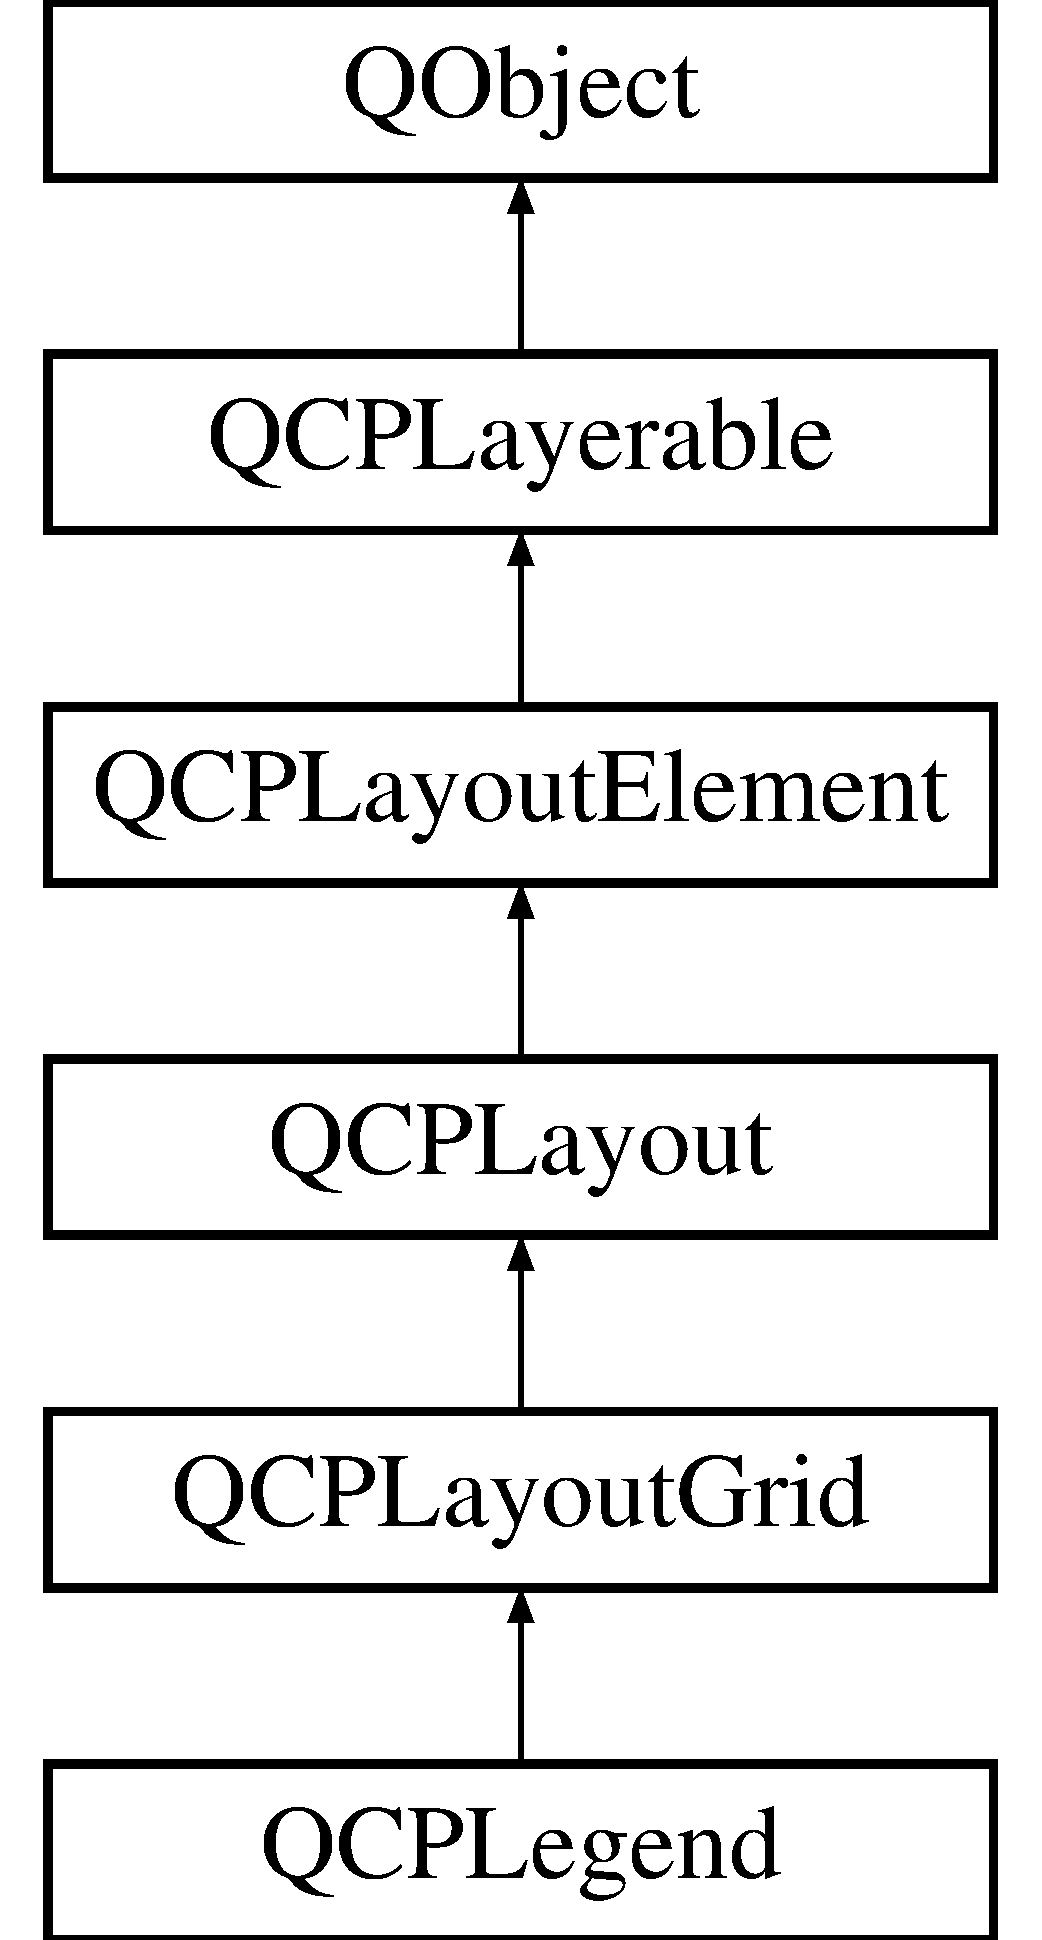
\includegraphics[height=6.000000cm]{class_q_c_p_layout_grid}
\end{center}
\end{figure}
\subsection*{Public Member Functions}
\begin{DoxyCompactItemize}
\item 
\hyperlink{class_q_c_p_layout_grid_ab2a4c1587dc8aed4c41c509c8d8d2a64}{Q\+C\+P\+Layout\+Grid} ()
\item 
int \hyperlink{class_q_c_p_layout_grid_a19c66fd76cbce58a8e94f33797e0c0aa}{row\+Count} () const
\item 
int \hyperlink{class_q_c_p_layout_grid_a1a2962cbf45011405b64b913afa8e7a2}{column\+Count} () const
\item 
\hypertarget{class_q_c_p_layout_grid_a8e0e587c386bbcd1b94119f5f44c512d}{}\label{class_q_c_p_layout_grid_a8e0e587c386bbcd1b94119f5f44c512d} 
Q\+List$<$ double $>$ {\bfseries column\+Stretch\+Factors} () const
\item 
\hypertarget{class_q_c_p_layout_grid_aa33408586427e77e05f79defde7f3568}{}\label{class_q_c_p_layout_grid_aa33408586427e77e05f79defde7f3568} 
Q\+List$<$ double $>$ {\bfseries row\+Stretch\+Factors} () const
\item 
\hypertarget{class_q_c_p_layout_grid_adcf4c387d5996bf6e4ae0ed26138247e}{}\label{class_q_c_p_layout_grid_adcf4c387d5996bf6e4ae0ed26138247e} 
int {\bfseries column\+Spacing} () const
\item 
\hypertarget{class_q_c_p_layout_grid_a4cb6c680505cd0ce6f85b9e217fd2cd0}{}\label{class_q_c_p_layout_grid_a4cb6c680505cd0ce6f85b9e217fd2cd0} 
int {\bfseries row\+Spacing} () const
\item 
void \hyperlink{class_q_c_p_layout_grid_ae38f31a71687b9d7ee3104852528fb50}{set\+Column\+Stretch\+Factor} (int column, double factor)
\item 
void \hyperlink{class_q_c_p_layout_grid_a6c2591d1a7e2534ce036989543b49e57}{set\+Column\+Stretch\+Factors} (const Q\+List$<$ double $>$ \&factors)
\item 
void \hyperlink{class_q_c_p_layout_grid_a7b0273de5369bd93d942edbaf5b166ec}{set\+Row\+Stretch\+Factor} (int row, double factor)
\item 
void \hyperlink{class_q_c_p_layout_grid_a200b45f9c908f96ebadaa3c8d87a2782}{set\+Row\+Stretch\+Factors} (const Q\+List$<$ double $>$ \&factors)
\item 
void \hyperlink{class_q_c_p_layout_grid_a3a49272aba32bb0fddc3bb2a45a3dba0}{set\+Column\+Spacing} (int pixels)
\item 
void \hyperlink{class_q_c_p_layout_grid_aaef2cd2d456197ee06a208793678e436}{set\+Row\+Spacing} (int pixels)
\item 
\hypertarget{class_q_c_p_layout_grid_a07f8dd7d3d61d7345026621d446042a4}{}\label{class_q_c_p_layout_grid_a07f8dd7d3d61d7345026621d446042a4} 
virtual void {\bfseries update\+Layout} ()
\item 
virtual int \hyperlink{class_q_c_p_layout_grid_a77f194843d037e0da6d5f3170acdf3a2}{element\+Count} () const
\item 
virtual \hyperlink{class_q_c_p_layout_element}{Q\+C\+P\+Layout\+Element} $\ast$ \hyperlink{class_q_c_p_layout_grid_a97672ecc379cb3a09639926ba9980297}{element\+At} (int index) const
\item 
virtual \hyperlink{class_q_c_p_layout_element}{Q\+C\+P\+Layout\+Element} $\ast$ \hyperlink{class_q_c_p_layout_grid_acc1277394ff8a6432e111ff9463e6375}{take\+At} (int index)
\item 
virtual bool \hyperlink{class_q_c_p_layout_grid_a666a9fe9e92054436f9b66eba25cca0c}{take} (\hyperlink{class_q_c_p_layout_element}{Q\+C\+P\+Layout\+Element} $\ast$\hyperlink{class_q_c_p_layout_grid_a602b426609b4411cf6a93c3ddf3a381a}{element})
\item 
virtual Q\+List$<$ \hyperlink{class_q_c_p_layout_element}{Q\+C\+P\+Layout\+Element} $\ast$ $>$ \hyperlink{class_q_c_p_layout_grid_a20a745d013de4c89cf5de8004a5a36f7}{elements} (bool recursive) const
\item 
virtual void \hyperlink{class_q_c_p_layout_grid_a08bba60e4acd20165526a8fd7f986b58}{simplify} ()
\item 
virtual Q\+Size \hyperlink{class_q_c_p_layout_grid_a9ef4b0d626708a1ada2cfea3a5973b80}{minimum\+Size\+Hint} () const
\item 
virtual Q\+Size \hyperlink{class_q_c_p_layout_grid_a3720d1b79931b2bdec3f2158a5f0181c}{maximum\+Size\+Hint} () const
\item 
\hyperlink{class_q_c_p_layout_element}{Q\+C\+P\+Layout\+Element} $\ast$ \hyperlink{class_q_c_p_layout_grid_a602b426609b4411cf6a93c3ddf3a381a}{element} (int row, int column) const
\item 
bool \hyperlink{class_q_c_p_layout_grid_adff1a2ca691ed83d2d24a4cd1fe17012}{add\+Element} (int row, int column, \hyperlink{class_q_c_p_layout_element}{Q\+C\+P\+Layout\+Element} $\ast$\hyperlink{class_q_c_p_layout_grid_a602b426609b4411cf6a93c3ddf3a381a}{element})
\item 
bool \hyperlink{class_q_c_p_layout_grid_ab0cf4f7edc9414a3bfaddac0f46dc0a0}{has\+Element} (int row, int column)
\item 
void \hyperlink{class_q_c_p_layout_grid_a886c0dcbabd51a45da399e044552b685}{expand\+To} (int new\+Row\+Count, int new\+Column\+Count)
\item 
void \hyperlink{class_q_c_p_layout_grid_a48af3dd7c3a653d9c3d7dd99bd02e838}{insert\+Row} (int new\+Index)
\item 
void \hyperlink{class_q_c_p_layout_grid_a1e880a321dbe8b43b471ccd764433dc4}{insert\+Column} (int new\+Index)
\end{DoxyCompactItemize}
\subsection*{Protected Member Functions}
\begin{DoxyCompactItemize}
\item 
\hypertarget{class_q_c_p_layout_grid_a4b9a251919936f127a63fc1b9911cd4e}{}\label{class_q_c_p_layout_grid_a4b9a251919936f127a63fc1b9911cd4e} 
void {\bfseries get\+Minimum\+Row\+Col\+Sizes} (Q\+Vector$<$ int $>$ $\ast$min\+Col\+Widths, Q\+Vector$<$ int $>$ $\ast$min\+Row\+Heights) const
\item 
\hypertarget{class_q_c_p_layout_grid_a9be77011ec5b5dfbe7fbda126659e1eb}{}\label{class_q_c_p_layout_grid_a9be77011ec5b5dfbe7fbda126659e1eb} 
void {\bfseries get\+Maximum\+Row\+Col\+Sizes} (Q\+Vector$<$ int $>$ $\ast$max\+Col\+Widths, Q\+Vector$<$ int $>$ $\ast$max\+Row\+Heights) const
\end{DoxyCompactItemize}
\subsection*{Protected Attributes}
\begin{DoxyCompactItemize}
\item 
\hypertarget{class_q_c_p_layout_grid_a3577d3855bf8ad20ef9079291a49f397}{}\label{class_q_c_p_layout_grid_a3577d3855bf8ad20ef9079291a49f397} 
Q\+List$<$ Q\+List$<$ \hyperlink{class_q_c_p_layout_element}{Q\+C\+P\+Layout\+Element} $\ast$ $>$ $>$ {\bfseries m\+Elements}
\item 
\hypertarget{class_q_c_p_layout_grid_ac6aabe62339f94f18b9f8adab94b1840}{}\label{class_q_c_p_layout_grid_ac6aabe62339f94f18b9f8adab94b1840} 
Q\+List$<$ double $>$ {\bfseries m\+Column\+Stretch\+Factors}
\item 
\hypertarget{class_q_c_p_layout_grid_a36c85a7eaf342680fb9b8a4977486f16}{}\label{class_q_c_p_layout_grid_a36c85a7eaf342680fb9b8a4977486f16} 
Q\+List$<$ double $>$ {\bfseries m\+Row\+Stretch\+Factors}
\item 
\hypertarget{class_q_c_p_layout_grid_ae9ac48f0791be07ead0a96dbd5622770}{}\label{class_q_c_p_layout_grid_ae9ac48f0791be07ead0a96dbd5622770} 
int {\bfseries m\+Column\+Spacing}
\item 
\hypertarget{class_q_c_p_layout_grid_a8b67f183f4645739cc4c794d75843b40}{}\label{class_q_c_p_layout_grid_a8b67f183f4645739cc4c794d75843b40} 
int {\bfseries m\+Row\+Spacing}
\end{DoxyCompactItemize}
\subsection*{Additional Inherited Members}


\subsection{Detailed Description}
A layout that arranges child elements in a grid. 

Elements are laid out in a grid with configurable stretch factors (\hyperlink{class_q_c_p_layout_grid_ae38f31a71687b9d7ee3104852528fb50}{set\+Column\+Stretch\+Factor}, \hyperlink{class_q_c_p_layout_grid_a7b0273de5369bd93d942edbaf5b166ec}{set\+Row\+Stretch\+Factor}) and spacing (\hyperlink{class_q_c_p_layout_grid_a3a49272aba32bb0fddc3bb2a45a3dba0}{set\+Column\+Spacing}, \hyperlink{class_q_c_p_layout_grid_aaef2cd2d456197ee06a208793678e436}{set\+Row\+Spacing}).

Elements can be added to cells via \hyperlink{class_q_c_p_layout_grid_adff1a2ca691ed83d2d24a4cd1fe17012}{add\+Element}. The grid is expanded if the specified row or column doesn\textquotesingle{}t exist yet. Whether a cell contains a valid layout element can be checked with \hyperlink{class_q_c_p_layout_grid_ab0cf4f7edc9414a3bfaddac0f46dc0a0}{has\+Element}, that element can be retrieved with \hyperlink{class_q_c_p_layout_grid_a602b426609b4411cf6a93c3ddf3a381a}{element}. If rows and columns that only have empty cells shall be removed, call \hyperlink{class_q_c_p_layout_grid_a08bba60e4acd20165526a8fd7f986b58}{simplify}. Removal of elements is either done by just adding the element to a different layout or by using the \hyperlink{class_q_c_p_layout}{Q\+C\+P\+Layout} interface \hyperlink{class_q_c_p_layout_grid_a666a9fe9e92054436f9b66eba25cca0c}{take} or \hyperlink{class_q_c_p_layout_a6c58f537d8086f352576ab7c5b15d0bc}{remove}.

Row and column insertion can be performed with \hyperlink{class_q_c_p_layout_grid_a48af3dd7c3a653d9c3d7dd99bd02e838}{insert\+Row} and \hyperlink{class_q_c_p_layout_grid_a1e880a321dbe8b43b471ccd764433dc4}{insert\+Column}. 

\subsection{Constructor \& Destructor Documentation}
\hypertarget{class_q_c_p_layout_grid_ab2a4c1587dc8aed4c41c509c8d8d2a64}{}\label{class_q_c_p_layout_grid_ab2a4c1587dc8aed4c41c509c8d8d2a64} 
\index{Q\+C\+P\+Layout\+Grid@{Q\+C\+P\+Layout\+Grid}!Q\+C\+P\+Layout\+Grid@{Q\+C\+P\+Layout\+Grid}}
\index{Q\+C\+P\+Layout\+Grid@{Q\+C\+P\+Layout\+Grid}!Q\+C\+P\+Layout\+Grid@{Q\+C\+P\+Layout\+Grid}}
\subsubsection{\texorpdfstring{Q\+C\+P\+Layout\+Grid()}{QCPLayoutGrid()}}
{\footnotesize\ttfamily Q\+C\+P\+Layout\+Grid\+::\+Q\+C\+P\+Layout\+Grid (\begin{DoxyParamCaption}{ }\end{DoxyParamCaption})\hspace{0.3cm}{\ttfamily [explicit]}}

Creates an instance of \hyperlink{class_q_c_p_layout_grid}{Q\+C\+P\+Layout\+Grid} and sets default values. 

\subsection{Member Function Documentation}
\hypertarget{class_q_c_p_layout_grid_adff1a2ca691ed83d2d24a4cd1fe17012}{}\label{class_q_c_p_layout_grid_adff1a2ca691ed83d2d24a4cd1fe17012} 
\index{Q\+C\+P\+Layout\+Grid@{Q\+C\+P\+Layout\+Grid}!add\+Element@{add\+Element}}
\index{add\+Element@{add\+Element}!Q\+C\+P\+Layout\+Grid@{Q\+C\+P\+Layout\+Grid}}
\subsubsection{\texorpdfstring{add\+Element()}{addElement()}}
{\footnotesize\ttfamily bool Q\+C\+P\+Layout\+Grid\+::add\+Element (\begin{DoxyParamCaption}\item[{int}]{row,  }\item[{int}]{column,  }\item[{\hyperlink{class_q_c_p_layout_element}{Q\+C\+P\+Layout\+Element} $\ast$}]{element }\end{DoxyParamCaption})}

Adds the {\itshape element} to cell with {\itshape row} and {\itshape column}. If {\itshape element} is already in a layout, it is first removed from there. If {\itshape row} or {\itshape column} don\textquotesingle{}t exist yet, the layout is expanded accordingly.

Returns true if the element was added successfully, i.\+e. if the cell at {\itshape row} and {\itshape column} didn\textquotesingle{}t already have an element.

\begin{DoxySeeAlso}{See also}
\hyperlink{class_q_c_p_layout_grid_a602b426609b4411cf6a93c3ddf3a381a}{element}, \hyperlink{class_q_c_p_layout_grid_ab0cf4f7edc9414a3bfaddac0f46dc0a0}{has\+Element}, \hyperlink{class_q_c_p_layout_grid_a666a9fe9e92054436f9b66eba25cca0c}{take}, \hyperlink{class_q_c_p_layout_a6c58f537d8086f352576ab7c5b15d0bc}{remove} 
\end{DoxySeeAlso}
\hypertarget{class_q_c_p_layout_grid_a1a2962cbf45011405b64b913afa8e7a2}{}\label{class_q_c_p_layout_grid_a1a2962cbf45011405b64b913afa8e7a2} 
\index{Q\+C\+P\+Layout\+Grid@{Q\+C\+P\+Layout\+Grid}!column\+Count@{column\+Count}}
\index{column\+Count@{column\+Count}!Q\+C\+P\+Layout\+Grid@{Q\+C\+P\+Layout\+Grid}}
\subsubsection{\texorpdfstring{column\+Count()}{columnCount()}}
{\footnotesize\ttfamily int Q\+C\+P\+Layout\+Grid\+::column\+Count (\begin{DoxyParamCaption}{ }\end{DoxyParamCaption}) const}

Returns the number of columns in the layout.

\begin{DoxySeeAlso}{See also}
\hyperlink{class_q_c_p_layout_grid_a19c66fd76cbce58a8e94f33797e0c0aa}{row\+Count} 
\end{DoxySeeAlso}
\hypertarget{class_q_c_p_layout_grid_a602b426609b4411cf6a93c3ddf3a381a}{}\label{class_q_c_p_layout_grid_a602b426609b4411cf6a93c3ddf3a381a} 
\index{Q\+C\+P\+Layout\+Grid@{Q\+C\+P\+Layout\+Grid}!element@{element}}
\index{element@{element}!Q\+C\+P\+Layout\+Grid@{Q\+C\+P\+Layout\+Grid}}
\subsubsection{\texorpdfstring{element()}{element()}}
{\footnotesize\ttfamily \hyperlink{class_q_c_p_layout_element}{Q\+C\+P\+Layout\+Element} $\ast$ Q\+C\+P\+Layout\+Grid\+::element (\begin{DoxyParamCaption}\item[{int}]{row,  }\item[{int}]{column }\end{DoxyParamCaption}) const}

Returns the element in the cell in {\itshape row} and {\itshape column}.

Returns 0 if either the row/column is invalid or if the cell is empty. In those cases, a q\+Debug message is printed. To check whether a cell exists and isn\textquotesingle{}t empty, use \hyperlink{class_q_c_p_layout_grid_ab0cf4f7edc9414a3bfaddac0f46dc0a0}{has\+Element}.

\begin{DoxySeeAlso}{See also}
\hyperlink{class_q_c_p_layout_grid_adff1a2ca691ed83d2d24a4cd1fe17012}{add\+Element}, \hyperlink{class_q_c_p_layout_grid_ab0cf4f7edc9414a3bfaddac0f46dc0a0}{has\+Element} 
\end{DoxySeeAlso}
\hypertarget{class_q_c_p_layout_grid_a97672ecc379cb3a09639926ba9980297}{}\label{class_q_c_p_layout_grid_a97672ecc379cb3a09639926ba9980297} 
\index{Q\+C\+P\+Layout\+Grid@{Q\+C\+P\+Layout\+Grid}!element\+At@{element\+At}}
\index{element\+At@{element\+At}!Q\+C\+P\+Layout\+Grid@{Q\+C\+P\+Layout\+Grid}}
\subsubsection{\texorpdfstring{element\+At()}{elementAt()}}
{\footnotesize\ttfamily \hyperlink{class_q_c_p_layout_element}{Q\+C\+P\+Layout\+Element} $\ast$ Q\+C\+P\+Layout\+Grid\+::element\+At (\begin{DoxyParamCaption}\item[{int}]{index }\end{DoxyParamCaption}) const\hspace{0.3cm}{\ttfamily [virtual]}}

Returns the element in the cell with the given {\itshape index}. If {\itshape index} is invalid, returns 0.

Note that even if {\itshape index} is valid, the respective cell may be empty in some layouts (e.\+g. \hyperlink{class_q_c_p_layout_grid}{Q\+C\+P\+Layout\+Grid}), so this function may return 0 in those cases. You may use this function to check whether a cell is empty or not.

\begin{DoxySeeAlso}{See also}
\hyperlink{class_q_c_p_layout_grid_a20a745d013de4c89cf5de8004a5a36f7}{elements}, \hyperlink{class_q_c_p_layout_grid_a77f194843d037e0da6d5f3170acdf3a2}{element\+Count}, \hyperlink{class_q_c_p_layout_grid_acc1277394ff8a6432e111ff9463e6375}{take\+At} 
\end{DoxySeeAlso}


Implements \hyperlink{class_q_c_p_layout_afa73ca7d859f8a3ee5c73c9b353d2a56}{Q\+C\+P\+Layout}.

\hypertarget{class_q_c_p_layout_grid_a77f194843d037e0da6d5f3170acdf3a2}{}\label{class_q_c_p_layout_grid_a77f194843d037e0da6d5f3170acdf3a2} 
\index{Q\+C\+P\+Layout\+Grid@{Q\+C\+P\+Layout\+Grid}!element\+Count@{element\+Count}}
\index{element\+Count@{element\+Count}!Q\+C\+P\+Layout\+Grid@{Q\+C\+P\+Layout\+Grid}}
\subsubsection{\texorpdfstring{element\+Count()}{elementCount()}}
{\footnotesize\ttfamily int Q\+C\+P\+Layout\+Grid\+::element\+Count (\begin{DoxyParamCaption}{ }\end{DoxyParamCaption}) const\hspace{0.3cm}{\ttfamily [virtual]}}

Returns the number of elements/cells in the layout.

\begin{DoxySeeAlso}{See also}
\hyperlink{class_q_c_p_layout_grid_a20a745d013de4c89cf5de8004a5a36f7}{elements}, \hyperlink{class_q_c_p_layout_grid_a97672ecc379cb3a09639926ba9980297}{element\+At} 
\end{DoxySeeAlso}


Implements \hyperlink{class_q_c_p_layout_a39d3e9ef5d9b82ab1885ba1cb9597e56}{Q\+C\+P\+Layout}.

\hypertarget{class_q_c_p_layout_grid_a20a745d013de4c89cf5de8004a5a36f7}{}\label{class_q_c_p_layout_grid_a20a745d013de4c89cf5de8004a5a36f7} 
\index{Q\+C\+P\+Layout\+Grid@{Q\+C\+P\+Layout\+Grid}!elements@{elements}}
\index{elements@{elements}!Q\+C\+P\+Layout\+Grid@{Q\+C\+P\+Layout\+Grid}}
\subsubsection{\texorpdfstring{elements()}{elements()}}
{\footnotesize\ttfamily Q\+List$<$ \hyperlink{class_q_c_p_layout_element}{Q\+C\+P\+Layout\+Element} $\ast$ $>$ Q\+C\+P\+Layout\+Grid\+::elements (\begin{DoxyParamCaption}\item[{bool}]{recursive }\end{DoxyParamCaption}) const\hspace{0.3cm}{\ttfamily [virtual]}}

Returns a list of all child elements in this layout element. If {\itshape recursive} is true, all sub-\/child elements are included in the list, too.

\begin{DoxyWarning}{Warning}
There may be entries with value 0 in the returned list. (For example, \hyperlink{class_q_c_p_layout_grid}{Q\+C\+P\+Layout\+Grid} may have empty cells which yield 0 at the respective index.) 
\end{DoxyWarning}


Reimplemented from \hyperlink{class_q_c_p_layout_adc9ebc73fc215f9cc22796712a251ff4}{Q\+C\+P\+Layout}.

\hypertarget{class_q_c_p_layout_grid_a886c0dcbabd51a45da399e044552b685}{}\label{class_q_c_p_layout_grid_a886c0dcbabd51a45da399e044552b685} 
\index{Q\+C\+P\+Layout\+Grid@{Q\+C\+P\+Layout\+Grid}!expand\+To@{expand\+To}}
\index{expand\+To@{expand\+To}!Q\+C\+P\+Layout\+Grid@{Q\+C\+P\+Layout\+Grid}}
\subsubsection{\texorpdfstring{expand\+To()}{expandTo()}}
{\footnotesize\ttfamily void Q\+C\+P\+Layout\+Grid\+::expand\+To (\begin{DoxyParamCaption}\item[{int}]{new\+Row\+Count,  }\item[{int}]{new\+Column\+Count }\end{DoxyParamCaption})}

Expands the layout to have {\itshape new\+Row\+Count} rows and {\itshape new\+Column\+Count} columns. So the last valid row index will be {\itshape new\+Row\+Count-\/1}, the last valid column index will be {\itshape new\+Column\+Count-\/1}.

If the current column/row count is already larger or equal to {\itshape new\+Column\+Count/{\itshape new\+Row\+Count},} this function does nothing in that dimension.

Newly created cells are empty, new rows and columns have the stretch factor 1.

Note that upon a call to \hyperlink{class_q_c_p_layout_grid_adff1a2ca691ed83d2d24a4cd1fe17012}{add\+Element}, the layout is expanded automatically to contain the specified row and column, using this function.

\begin{DoxySeeAlso}{See also}
\hyperlink{class_q_c_p_layout_grid_a08bba60e4acd20165526a8fd7f986b58}{simplify} 
\end{DoxySeeAlso}
\hypertarget{class_q_c_p_layout_grid_ab0cf4f7edc9414a3bfaddac0f46dc0a0}{}\label{class_q_c_p_layout_grid_ab0cf4f7edc9414a3bfaddac0f46dc0a0} 
\index{Q\+C\+P\+Layout\+Grid@{Q\+C\+P\+Layout\+Grid}!has\+Element@{has\+Element}}
\index{has\+Element@{has\+Element}!Q\+C\+P\+Layout\+Grid@{Q\+C\+P\+Layout\+Grid}}
\subsubsection{\texorpdfstring{has\+Element()}{hasElement()}}
{\footnotesize\ttfamily bool Q\+C\+P\+Layout\+Grid\+::has\+Element (\begin{DoxyParamCaption}\item[{int}]{row,  }\item[{int}]{column }\end{DoxyParamCaption})}

Returns whether the cell at {\itshape row} and {\itshape column} exists and contains a valid element, i.\+e. isn\textquotesingle{}t empty.

\begin{DoxySeeAlso}{See also}
\hyperlink{class_q_c_p_layout_grid_a602b426609b4411cf6a93c3ddf3a381a}{element} 
\end{DoxySeeAlso}
\hypertarget{class_q_c_p_layout_grid_a1e880a321dbe8b43b471ccd764433dc4}{}\label{class_q_c_p_layout_grid_a1e880a321dbe8b43b471ccd764433dc4} 
\index{Q\+C\+P\+Layout\+Grid@{Q\+C\+P\+Layout\+Grid}!insert\+Column@{insert\+Column}}
\index{insert\+Column@{insert\+Column}!Q\+C\+P\+Layout\+Grid@{Q\+C\+P\+Layout\+Grid}}
\subsubsection{\texorpdfstring{insert\+Column()}{insertColumn()}}
{\footnotesize\ttfamily void Q\+C\+P\+Layout\+Grid\+::insert\+Column (\begin{DoxyParamCaption}\item[{int}]{new\+Index }\end{DoxyParamCaption})}

Inserts a new column with empty cells at the column index {\itshape new\+Index}. Valid values for {\itshape new\+Index} range from 0 (inserts a row at the left) to {\itshape row\+Count} (appends a row at the right).

\begin{DoxySeeAlso}{See also}
\hyperlink{class_q_c_p_layout_grid_a48af3dd7c3a653d9c3d7dd99bd02e838}{insert\+Row} 
\end{DoxySeeAlso}
\hypertarget{class_q_c_p_layout_grid_a48af3dd7c3a653d9c3d7dd99bd02e838}{}\label{class_q_c_p_layout_grid_a48af3dd7c3a653d9c3d7dd99bd02e838} 
\index{Q\+C\+P\+Layout\+Grid@{Q\+C\+P\+Layout\+Grid}!insert\+Row@{insert\+Row}}
\index{insert\+Row@{insert\+Row}!Q\+C\+P\+Layout\+Grid@{Q\+C\+P\+Layout\+Grid}}
\subsubsection{\texorpdfstring{insert\+Row()}{insertRow()}}
{\footnotesize\ttfamily void Q\+C\+P\+Layout\+Grid\+::insert\+Row (\begin{DoxyParamCaption}\item[{int}]{new\+Index }\end{DoxyParamCaption})}

Inserts a new row with empty cells at the row index {\itshape new\+Index}. Valid values for {\itshape new\+Index} range from 0 (inserts a row at the top) to {\itshape row\+Count} (appends a row at the bottom).

\begin{DoxySeeAlso}{See also}
\hyperlink{class_q_c_p_layout_grid_a1e880a321dbe8b43b471ccd764433dc4}{insert\+Column} 
\end{DoxySeeAlso}
\hypertarget{class_q_c_p_layout_grid_a3720d1b79931b2bdec3f2158a5f0181c}{}\label{class_q_c_p_layout_grid_a3720d1b79931b2bdec3f2158a5f0181c} 
\index{Q\+C\+P\+Layout\+Grid@{Q\+C\+P\+Layout\+Grid}!maximum\+Size\+Hint@{maximum\+Size\+Hint}}
\index{maximum\+Size\+Hint@{maximum\+Size\+Hint}!Q\+C\+P\+Layout\+Grid@{Q\+C\+P\+Layout\+Grid}}
\subsubsection{\texorpdfstring{maximum\+Size\+Hint()}{maximumSizeHint()}}
{\footnotesize\ttfamily Q\+Size Q\+C\+P\+Layout\+Grid\+::maximum\+Size\+Hint (\begin{DoxyParamCaption}{ }\end{DoxyParamCaption}) const\hspace{0.3cm}{\ttfamily [virtual]}}

Returns the maximum size this layout element (the inner \hyperlink{class_q_c_p_layout_element_a208effccfe2cca4a0eaf9393e60f2dd4}{rect}) may be expanded to.

if a maximum size (\hyperlink{class_q_c_p_layout_element_a74eb5280a737ab44833d506db65efd95}{set\+Maximum\+Size}) was not set manually, parent layouts consult this function to determine the maximum allowed size of this layout element. (A manual maximum size is considered set if it is smaller than Qt\textquotesingle{}s Q\+W\+I\+D\+G\+E\+T\+S\+I\+Z\+E\+\_\+\+M\+AX.) 

Reimplemented from \hyperlink{class_q_c_p_layout_element_ab5ce2ba22b36d9a3b70a1be562c326e5}{Q\+C\+P\+Layout\+Element}.

\hypertarget{class_q_c_p_layout_grid_a9ef4b0d626708a1ada2cfea3a5973b80}{}\label{class_q_c_p_layout_grid_a9ef4b0d626708a1ada2cfea3a5973b80} 
\index{Q\+C\+P\+Layout\+Grid@{Q\+C\+P\+Layout\+Grid}!minimum\+Size\+Hint@{minimum\+Size\+Hint}}
\index{minimum\+Size\+Hint@{minimum\+Size\+Hint}!Q\+C\+P\+Layout\+Grid@{Q\+C\+P\+Layout\+Grid}}
\subsubsection{\texorpdfstring{minimum\+Size\+Hint()}{minimumSizeHint()}}
{\footnotesize\ttfamily Q\+Size Q\+C\+P\+Layout\+Grid\+::minimum\+Size\+Hint (\begin{DoxyParamCaption}{ }\end{DoxyParamCaption}) const\hspace{0.3cm}{\ttfamily [virtual]}}

Returns the minimum size this layout element (the inner \hyperlink{class_q_c_p_layout_element_a208effccfe2cca4a0eaf9393e60f2dd4}{rect}) may be compressed to.

if a minimum size (\hyperlink{class_q_c_p_layout_element_a5dd29a3c8bc88440c97c06b67be7886b}{set\+Minimum\+Size}) was not set manually, parent layouts consult this function to determine the minimum allowed size of this layout element. (A manual minimum size is considered set if it is non-\/zero.) 

Reimplemented from \hyperlink{class_q_c_p_layout_element_ab3fdb5c9a5189bb2dac10d4d25329cd8}{Q\+C\+P\+Layout\+Element}.

\hypertarget{class_q_c_p_layout_grid_a19c66fd76cbce58a8e94f33797e0c0aa}{}\label{class_q_c_p_layout_grid_a19c66fd76cbce58a8e94f33797e0c0aa} 
\index{Q\+C\+P\+Layout\+Grid@{Q\+C\+P\+Layout\+Grid}!row\+Count@{row\+Count}}
\index{row\+Count@{row\+Count}!Q\+C\+P\+Layout\+Grid@{Q\+C\+P\+Layout\+Grid}}
\subsubsection{\texorpdfstring{row\+Count()}{rowCount()}}
{\footnotesize\ttfamily int Q\+C\+P\+Layout\+Grid\+::row\+Count (\begin{DoxyParamCaption}{ }\end{DoxyParamCaption}) const}

Returns the number of rows in the layout.

\begin{DoxySeeAlso}{See also}
\hyperlink{class_q_c_p_layout_grid_a1a2962cbf45011405b64b913afa8e7a2}{column\+Count} 
\end{DoxySeeAlso}
\hypertarget{class_q_c_p_layout_grid_a3a49272aba32bb0fddc3bb2a45a3dba0}{}\label{class_q_c_p_layout_grid_a3a49272aba32bb0fddc3bb2a45a3dba0} 
\index{Q\+C\+P\+Layout\+Grid@{Q\+C\+P\+Layout\+Grid}!set\+Column\+Spacing@{set\+Column\+Spacing}}
\index{set\+Column\+Spacing@{set\+Column\+Spacing}!Q\+C\+P\+Layout\+Grid@{Q\+C\+P\+Layout\+Grid}}
\subsubsection{\texorpdfstring{set\+Column\+Spacing()}{setColumnSpacing()}}
{\footnotesize\ttfamily void Q\+C\+P\+Layout\+Grid\+::set\+Column\+Spacing (\begin{DoxyParamCaption}\item[{int}]{pixels }\end{DoxyParamCaption})}

Sets the gap that is left blank between columns to {\itshape pixels}.

\begin{DoxySeeAlso}{See also}
\hyperlink{class_q_c_p_layout_grid_aaef2cd2d456197ee06a208793678e436}{set\+Row\+Spacing} 
\end{DoxySeeAlso}
\hypertarget{class_q_c_p_layout_grid_ae38f31a71687b9d7ee3104852528fb50}{}\label{class_q_c_p_layout_grid_ae38f31a71687b9d7ee3104852528fb50} 
\index{Q\+C\+P\+Layout\+Grid@{Q\+C\+P\+Layout\+Grid}!set\+Column\+Stretch\+Factor@{set\+Column\+Stretch\+Factor}}
\index{set\+Column\+Stretch\+Factor@{set\+Column\+Stretch\+Factor}!Q\+C\+P\+Layout\+Grid@{Q\+C\+P\+Layout\+Grid}}
\subsubsection{\texorpdfstring{set\+Column\+Stretch\+Factor()}{setColumnStretchFactor()}}
{\footnotesize\ttfamily void Q\+C\+P\+Layout\+Grid\+::set\+Column\+Stretch\+Factor (\begin{DoxyParamCaption}\item[{int}]{column,  }\item[{double}]{factor }\end{DoxyParamCaption})}

Sets the stretch {\itshape factor} of {\itshape column}.

Stretch factors control the relative sizes of rows and columns. Cells will not be resized beyond their minimum and maximum widths/heights (\hyperlink{class_q_c_p_layout_element_a5dd29a3c8bc88440c97c06b67be7886b}{Q\+C\+P\+Layout\+Element\+::set\+Minimum\+Size}, \hyperlink{class_q_c_p_layout_element_a74eb5280a737ab44833d506db65efd95}{Q\+C\+P\+Layout\+Element\+::set\+Maximum\+Size}), regardless of the stretch factor.

The default stretch factor of newly created rows/columns is 1.

\begin{DoxySeeAlso}{See also}
\hyperlink{class_q_c_p_layout_grid_a6c2591d1a7e2534ce036989543b49e57}{set\+Column\+Stretch\+Factors}, \hyperlink{class_q_c_p_layout_grid_a7b0273de5369bd93d942edbaf5b166ec}{set\+Row\+Stretch\+Factor} 
\end{DoxySeeAlso}
\hypertarget{class_q_c_p_layout_grid_a6c2591d1a7e2534ce036989543b49e57}{}\label{class_q_c_p_layout_grid_a6c2591d1a7e2534ce036989543b49e57} 
\index{Q\+C\+P\+Layout\+Grid@{Q\+C\+P\+Layout\+Grid}!set\+Column\+Stretch\+Factors@{set\+Column\+Stretch\+Factors}}
\index{set\+Column\+Stretch\+Factors@{set\+Column\+Stretch\+Factors}!Q\+C\+P\+Layout\+Grid@{Q\+C\+P\+Layout\+Grid}}
\subsubsection{\texorpdfstring{set\+Column\+Stretch\+Factors()}{setColumnStretchFactors()}}
{\footnotesize\ttfamily void Q\+C\+P\+Layout\+Grid\+::set\+Column\+Stretch\+Factors (\begin{DoxyParamCaption}\item[{const Q\+List$<$ double $>$ \&}]{factors }\end{DoxyParamCaption})}

Sets the stretch {\itshape factors} of all columns. {\itshape factors} must have the size \hyperlink{class_q_c_p_layout_grid_a1a2962cbf45011405b64b913afa8e7a2}{column\+Count}.

Stretch factors control the relative sizes of rows and columns. Cells will not be resized beyond their minimum and maximum widths/heights (\hyperlink{class_q_c_p_layout_element_a5dd29a3c8bc88440c97c06b67be7886b}{Q\+C\+P\+Layout\+Element\+::set\+Minimum\+Size}, \hyperlink{class_q_c_p_layout_element_a74eb5280a737ab44833d506db65efd95}{Q\+C\+P\+Layout\+Element\+::set\+Maximum\+Size}), regardless of the stretch factor.

The default stretch factor of newly created rows/columns is 1.

\begin{DoxySeeAlso}{See also}
\hyperlink{class_q_c_p_layout_grid_ae38f31a71687b9d7ee3104852528fb50}{set\+Column\+Stretch\+Factor}, \hyperlink{class_q_c_p_layout_grid_a200b45f9c908f96ebadaa3c8d87a2782}{set\+Row\+Stretch\+Factors} 
\end{DoxySeeAlso}
\hypertarget{class_q_c_p_layout_grid_aaef2cd2d456197ee06a208793678e436}{}\label{class_q_c_p_layout_grid_aaef2cd2d456197ee06a208793678e436} 
\index{Q\+C\+P\+Layout\+Grid@{Q\+C\+P\+Layout\+Grid}!set\+Row\+Spacing@{set\+Row\+Spacing}}
\index{set\+Row\+Spacing@{set\+Row\+Spacing}!Q\+C\+P\+Layout\+Grid@{Q\+C\+P\+Layout\+Grid}}
\subsubsection{\texorpdfstring{set\+Row\+Spacing()}{setRowSpacing()}}
{\footnotesize\ttfamily void Q\+C\+P\+Layout\+Grid\+::set\+Row\+Spacing (\begin{DoxyParamCaption}\item[{int}]{pixels }\end{DoxyParamCaption})}

Sets the gap that is left blank between rows to {\itshape pixels}.

\begin{DoxySeeAlso}{See also}
\hyperlink{class_q_c_p_layout_grid_a3a49272aba32bb0fddc3bb2a45a3dba0}{set\+Column\+Spacing} 
\end{DoxySeeAlso}
\hypertarget{class_q_c_p_layout_grid_a7b0273de5369bd93d942edbaf5b166ec}{}\label{class_q_c_p_layout_grid_a7b0273de5369bd93d942edbaf5b166ec} 
\index{Q\+C\+P\+Layout\+Grid@{Q\+C\+P\+Layout\+Grid}!set\+Row\+Stretch\+Factor@{set\+Row\+Stretch\+Factor}}
\index{set\+Row\+Stretch\+Factor@{set\+Row\+Stretch\+Factor}!Q\+C\+P\+Layout\+Grid@{Q\+C\+P\+Layout\+Grid}}
\subsubsection{\texorpdfstring{set\+Row\+Stretch\+Factor()}{setRowStretchFactor()}}
{\footnotesize\ttfamily void Q\+C\+P\+Layout\+Grid\+::set\+Row\+Stretch\+Factor (\begin{DoxyParamCaption}\item[{int}]{row,  }\item[{double}]{factor }\end{DoxyParamCaption})}

Sets the stretch {\itshape factor} of {\itshape row}.

Stretch factors control the relative sizes of rows and columns. Cells will not be resized beyond their minimum and maximum widths/heights (\hyperlink{class_q_c_p_layout_element_a5dd29a3c8bc88440c97c06b67be7886b}{Q\+C\+P\+Layout\+Element\+::set\+Minimum\+Size}, \hyperlink{class_q_c_p_layout_element_a74eb5280a737ab44833d506db65efd95}{Q\+C\+P\+Layout\+Element\+::set\+Maximum\+Size}), regardless of the stretch factor.

The default stretch factor of newly created rows/columns is 1.

\begin{DoxySeeAlso}{See also}
\hyperlink{class_q_c_p_layout_grid_a6c2591d1a7e2534ce036989543b49e57}{set\+Column\+Stretch\+Factors}, \hyperlink{class_q_c_p_layout_grid_a7b0273de5369bd93d942edbaf5b166ec}{set\+Row\+Stretch\+Factor} 
\end{DoxySeeAlso}
\hypertarget{class_q_c_p_layout_grid_a200b45f9c908f96ebadaa3c8d87a2782}{}\label{class_q_c_p_layout_grid_a200b45f9c908f96ebadaa3c8d87a2782} 
\index{Q\+C\+P\+Layout\+Grid@{Q\+C\+P\+Layout\+Grid}!set\+Row\+Stretch\+Factors@{set\+Row\+Stretch\+Factors}}
\index{set\+Row\+Stretch\+Factors@{set\+Row\+Stretch\+Factors}!Q\+C\+P\+Layout\+Grid@{Q\+C\+P\+Layout\+Grid}}
\subsubsection{\texorpdfstring{set\+Row\+Stretch\+Factors()}{setRowStretchFactors()}}
{\footnotesize\ttfamily void Q\+C\+P\+Layout\+Grid\+::set\+Row\+Stretch\+Factors (\begin{DoxyParamCaption}\item[{const Q\+List$<$ double $>$ \&}]{factors }\end{DoxyParamCaption})}

Sets the stretch {\itshape factors} of all rows. {\itshape factors} must have the size \hyperlink{class_q_c_p_layout_grid_a19c66fd76cbce58a8e94f33797e0c0aa}{row\+Count}.

Stretch factors control the relative sizes of rows and columns. Cells will not be resized beyond their minimum and maximum widths/heights (\hyperlink{class_q_c_p_layout_element_a5dd29a3c8bc88440c97c06b67be7886b}{Q\+C\+P\+Layout\+Element\+::set\+Minimum\+Size}, \hyperlink{class_q_c_p_layout_element_a74eb5280a737ab44833d506db65efd95}{Q\+C\+P\+Layout\+Element\+::set\+Maximum\+Size}), regardless of the stretch factor.

The default stretch factor of newly created rows/columns is 1.

\begin{DoxySeeAlso}{See also}
\hyperlink{class_q_c_p_layout_grid_a7b0273de5369bd93d942edbaf5b166ec}{set\+Row\+Stretch\+Factor}, \hyperlink{class_q_c_p_layout_grid_a6c2591d1a7e2534ce036989543b49e57}{set\+Column\+Stretch\+Factors} 
\end{DoxySeeAlso}
\hypertarget{class_q_c_p_layout_grid_a08bba60e4acd20165526a8fd7f986b58}{}\label{class_q_c_p_layout_grid_a08bba60e4acd20165526a8fd7f986b58} 
\index{Q\+C\+P\+Layout\+Grid@{Q\+C\+P\+Layout\+Grid}!simplify@{simplify}}
\index{simplify@{simplify}!Q\+C\+P\+Layout\+Grid@{Q\+C\+P\+Layout\+Grid}}
\subsubsection{\texorpdfstring{simplify()}{simplify()}}
{\footnotesize\ttfamily void Q\+C\+P\+Layout\+Grid\+::simplify (\begin{DoxyParamCaption}{ }\end{DoxyParamCaption})\hspace{0.3cm}{\ttfamily [virtual]}}

Simplifies the layout by collapsing rows and columns which only contain empty cells. 

Reimplemented from \hyperlink{class_q_c_p_layout_a41e6ac049143866e8f8b4964efab01b2}{Q\+C\+P\+Layout}.

\hypertarget{class_q_c_p_layout_grid_a666a9fe9e92054436f9b66eba25cca0c}{}\label{class_q_c_p_layout_grid_a666a9fe9e92054436f9b66eba25cca0c} 
\index{Q\+C\+P\+Layout\+Grid@{Q\+C\+P\+Layout\+Grid}!take@{take}}
\index{take@{take}!Q\+C\+P\+Layout\+Grid@{Q\+C\+P\+Layout\+Grid}}
\subsubsection{\texorpdfstring{take()}{take()}}
{\footnotesize\ttfamily bool Q\+C\+P\+Layout\+Grid\+::take (\begin{DoxyParamCaption}\item[{\hyperlink{class_q_c_p_layout_element}{Q\+C\+P\+Layout\+Element} $\ast$}]{element }\end{DoxyParamCaption})\hspace{0.3cm}{\ttfamily [virtual]}}

Removes the specified {\itshape element} from the layout and returns true on success.

If the {\itshape element} isn\textquotesingle{}t in this layout, returns false.

Note that some layouts don\textquotesingle{}t remove the respective cell right away but leave an empty cell after successful removal of the layout element. To collapse empty cells, use \hyperlink{class_q_c_p_layout_grid_a08bba60e4acd20165526a8fd7f986b58}{simplify}.

\begin{DoxySeeAlso}{See also}
\hyperlink{class_q_c_p_layout_grid_acc1277394ff8a6432e111ff9463e6375}{take\+At} 
\end{DoxySeeAlso}


Implements \hyperlink{class_q_c_p_layout_ada26cd17e56472b0b4d7fbbc96873e4c}{Q\+C\+P\+Layout}.

\hypertarget{class_q_c_p_layout_grid_acc1277394ff8a6432e111ff9463e6375}{}\label{class_q_c_p_layout_grid_acc1277394ff8a6432e111ff9463e6375} 
\index{Q\+C\+P\+Layout\+Grid@{Q\+C\+P\+Layout\+Grid}!take\+At@{take\+At}}
\index{take\+At@{take\+At}!Q\+C\+P\+Layout\+Grid@{Q\+C\+P\+Layout\+Grid}}
\subsubsection{\texorpdfstring{take\+At()}{takeAt()}}
{\footnotesize\ttfamily \hyperlink{class_q_c_p_layout_element}{Q\+C\+P\+Layout\+Element} $\ast$ Q\+C\+P\+Layout\+Grid\+::take\+At (\begin{DoxyParamCaption}\item[{int}]{index }\end{DoxyParamCaption})\hspace{0.3cm}{\ttfamily [virtual]}}

Removes the element with the given {\itshape index} from the layout and returns it.

If the {\itshape index} is invalid or the cell with that index is empty, returns 0.

Note that some layouts don\textquotesingle{}t remove the respective cell right away but leave an empty cell after successful removal of the layout element. To collapse empty cells, use \hyperlink{class_q_c_p_layout_grid_a08bba60e4acd20165526a8fd7f986b58}{simplify}.

\begin{DoxySeeAlso}{See also}
\hyperlink{class_q_c_p_layout_grid_a97672ecc379cb3a09639926ba9980297}{element\+At}, \hyperlink{class_q_c_p_layout_grid_a666a9fe9e92054436f9b66eba25cca0c}{take} 
\end{DoxySeeAlso}


Implements \hyperlink{class_q_c_p_layout_a5a79621fa0a6eabb8b520cfc04fb601a}{Q\+C\+P\+Layout}.



The documentation for this class was generated from the following files\+:\begin{DoxyCompactItemize}
\item 
C\+:/\+Users/\+Jesse Jutson/\+Documents/\+Git\+Hub/\+F\+E\+S\+S\+G\+U\+I/\+F\+E\+S\+S-\/\+G\+U\+I/\hyperlink{qcustomplot_8h}{qcustomplot.\+h}\item 
C\+:/\+Users/\+Jesse Jutson/\+Documents/\+Git\+Hub/\+F\+E\+S\+S\+G\+U\+I/\+F\+E\+S\+S-\/\+G\+U\+I/\hyperlink{qcustomplot_8cpp}{qcustomplot.\+cpp}\end{DoxyCompactItemize}

\hypertarget{class_q_c_p_layout_inset}{}\section{Q\+C\+P\+Layout\+Inset Class Reference}
\label{class_q_c_p_layout_inset}\index{Q\+C\+P\+Layout\+Inset@{Q\+C\+P\+Layout\+Inset}}


A layout that places child elements aligned to the border or arbitrarily positioned.  


Inheritance diagram for Q\+C\+P\+Layout\+Inset\+:\begin{figure}[H]
\begin{center}
\leavevmode
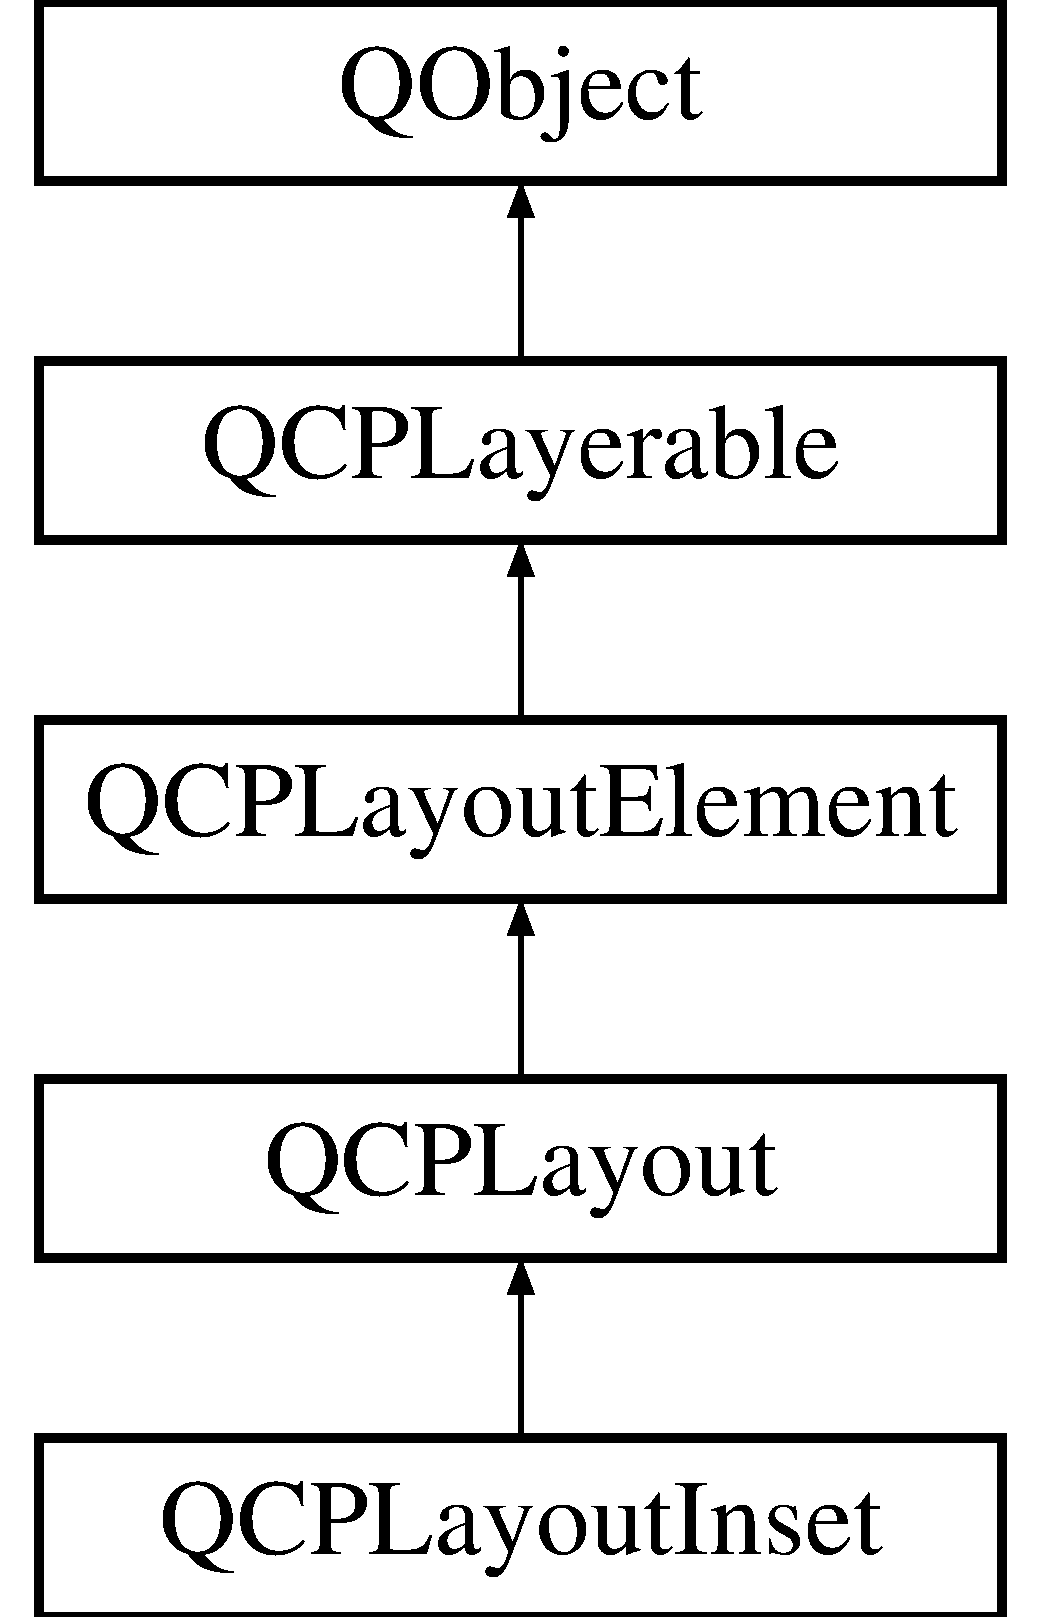
\includegraphics[height=5.000000cm]{class_q_c_p_layout_inset}
\end{center}
\end{figure}
\subsection*{Public Types}
\begin{DoxyCompactItemize}
\item 
enum \hyperlink{class_q_c_p_layout_inset_a8b9e17d9a2768293d2a7d72f5e298192}{Inset\+Placement} \{ \hyperlink{class_q_c_p_layout_inset_a8b9e17d9a2768293d2a7d72f5e298192aa4802986ea2cea457f932b115acba59e}{ip\+Free}, 
\hyperlink{class_q_c_p_layout_inset_a8b9e17d9a2768293d2a7d72f5e298192aa81e7df4a785ddee2229a8f47c46e817}{ip\+Border\+Aligned}
 \}
\end{DoxyCompactItemize}
\subsection*{Public Member Functions}
\begin{DoxyCompactItemize}
\item 
\hyperlink{class_q_c_p_layout_inset_a3ad984f3221735374cc5dee14356a7dd}{Q\+C\+P\+Layout\+Inset} ()
\item 
\hyperlink{class_q_c_p_layout_inset_a8b9e17d9a2768293d2a7d72f5e298192}{Inset\+Placement} \hyperlink{class_q_c_p_layout_inset_a6fcbd74ebbc45bfe64c604b2791aa57f}{inset\+Placement} (int index) const
\item 
Qt\+::\+Alignment \hyperlink{class_q_c_p_layout_inset_a5b33b66f0abbb4a7cc2f8aa6c94cf7f8}{inset\+Alignment} (int index) const
\item 
Q\+RectF \hyperlink{class_q_c_p_layout_inset_ab23099a46af17c31f4c40668f13c9de1}{inset\+Rect} (int index) const
\item 
void \hyperlink{class_q_c_p_layout_inset_a63298830744d5d8c5345511c00fd2144}{set\+Inset\+Placement} (int index, \hyperlink{class_q_c_p_layout_inset_a8b9e17d9a2768293d2a7d72f5e298192}{Inset\+Placement} placement)
\item 
void \hyperlink{class_q_c_p_layout_inset_a62882a4f9ad58bb0f53da12fde022abe}{set\+Inset\+Alignment} (int index, Qt\+::\+Alignment alignment)
\item 
void \hyperlink{class_q_c_p_layout_inset_aa487c8378a6f9533567a2e6430099dc3}{set\+Inset\+Rect} (int index, const Q\+RectF \&\hyperlink{class_q_c_p_layout_element_a208effccfe2cca4a0eaf9393e60f2dd4}{rect})
\item 
\hypertarget{class_q_c_p_layout_inset_a7b33fdd51b18e6db7cea9bfb2d263b4a}{}\label{class_q_c_p_layout_inset_a7b33fdd51b18e6db7cea9bfb2d263b4a} 
virtual void {\bfseries update\+Layout} ()
\item 
virtual int \hyperlink{class_q_c_p_layout_inset_a0398918a888fa7974a6776dc47fc5d2e}{element\+Count} () const
\item 
virtual \hyperlink{class_q_c_p_layout_element}{Q\+C\+P\+Layout\+Element} $\ast$ \hyperlink{class_q_c_p_layout_inset_a832e049f0bb32e7db0490a9c904098df}{element\+At} (int index) const
\item 
virtual \hyperlink{class_q_c_p_layout_element}{Q\+C\+P\+Layout\+Element} $\ast$ \hyperlink{class_q_c_p_layout_inset_ad6756a3b507e20496aaf7f5ca16c47d1}{take\+At} (int index)
\item 
virtual bool \hyperlink{class_q_c_p_layout_inset_a9ac707ccff650633b97f52dd5cddcf49}{take} (\hyperlink{class_q_c_p_layout_element}{Q\+C\+P\+Layout\+Element} $\ast$element)
\item 
virtual void \hyperlink{class_q_c_p_layout_inset_abb9eb23bf2d7c587a8abe02d065eae0a}{simplify} ()
\item 
virtual double \hyperlink{class_q_c_p_layout_inset_afcd56d5d1b8853838cdc535f1904f68a}{select\+Test} (const Q\+PointF \&pos, bool only\+Selectable, Q\+Variant $\ast$details=0) const
\item 
void \hyperlink{class_q_c_p_layout_inset_ad61529eb576af7f04dff94abb10c745a}{add\+Element} (\hyperlink{class_q_c_p_layout_element}{Q\+C\+P\+Layout\+Element} $\ast$element, Qt\+::\+Alignment alignment)
\item 
void \hyperlink{class_q_c_p_layout_inset_a8ff61fbee4a1f0ff45c398009d9f1e56}{add\+Element} (\hyperlink{class_q_c_p_layout_element}{Q\+C\+P\+Layout\+Element} $\ast$element, const Q\+RectF \&\hyperlink{class_q_c_p_layout_element_a208effccfe2cca4a0eaf9393e60f2dd4}{rect})
\end{DoxyCompactItemize}
\subsection*{Protected Attributes}
\begin{DoxyCompactItemize}
\item 
\hypertarget{class_q_c_p_layout_inset_a8fff7eae9a1be9a5c1e544fb379f682f}{}\label{class_q_c_p_layout_inset_a8fff7eae9a1be9a5c1e544fb379f682f} 
Q\+List$<$ \hyperlink{class_q_c_p_layout_element}{Q\+C\+P\+Layout\+Element} $\ast$ $>$ {\bfseries m\+Elements}
\item 
\hypertarget{class_q_c_p_layout_inset_a57a0a4e445cc78eada29765ecf092abe}{}\label{class_q_c_p_layout_inset_a57a0a4e445cc78eada29765ecf092abe} 
Q\+List$<$ \hyperlink{class_q_c_p_layout_inset_a8b9e17d9a2768293d2a7d72f5e298192}{Inset\+Placement} $>$ {\bfseries m\+Inset\+Placement}
\item 
\hypertarget{class_q_c_p_layout_inset_a55e9b84c310136ff985a6544184ab64a}{}\label{class_q_c_p_layout_inset_a55e9b84c310136ff985a6544184ab64a} 
Q\+List$<$ Qt\+::\+Alignment $>$ {\bfseries m\+Inset\+Alignment}
\item 
\hypertarget{class_q_c_p_layout_inset_aaa8f6b5029458f3d97a65239524a2b33}{}\label{class_q_c_p_layout_inset_aaa8f6b5029458f3d97a65239524a2b33} 
Q\+List$<$ Q\+RectF $>$ {\bfseries m\+Inset\+Rect}
\end{DoxyCompactItemize}
\subsection*{Additional Inherited Members}


\subsection{Detailed Description}
A layout that places child elements aligned to the border or arbitrarily positioned. 

Elements are placed either aligned to the border or at arbitrary position in the area of the layout. Which placement applies is controlled with the \hyperlink{class_q_c_p_layout_inset_a8b9e17d9a2768293d2a7d72f5e298192}{Inset\+Placement} (\hyperlink{class_q_c_p_layout_inset_a63298830744d5d8c5345511c00fd2144}{set\+Inset\+Placement}).

Elements are added via \hyperlink{class_q_c_p_layout_inset_ad61529eb576af7f04dff94abb10c745a}{add\+Element(\+Q\+C\+P\+Layout\+Element $\ast$element, Qt\+::\+Alignment alignment)} or \hyperlink{class_q_c_p_layout_inset_a8ff61fbee4a1f0ff45c398009d9f1e56}{add\+Element(\+Q\+C\+P\+Layout\+Element $\ast$element, const Q\+Rect\+F \&rect)}. If the first method is used, the inset placement will default to \hyperlink{class_q_c_p_layout_inset_a8b9e17d9a2768293d2a7d72f5e298192aa81e7df4a785ddee2229a8f47c46e817}{ip\+Border\+Aligned} and the element will be aligned according to the {\itshape alignment} parameter. The second method defaults to \hyperlink{class_q_c_p_layout_inset_a8b9e17d9a2768293d2a7d72f5e298192aa4802986ea2cea457f932b115acba59e}{ip\+Free} and allows placing elements at arbitrary position and size, defined by {\itshape rect}.

The alignment or rect can be set via \hyperlink{class_q_c_p_layout_inset_a62882a4f9ad58bb0f53da12fde022abe}{set\+Inset\+Alignment} or \hyperlink{class_q_c_p_layout_inset_aa487c8378a6f9533567a2e6430099dc3}{set\+Inset\+Rect}, respectively.

This is the layout that every \hyperlink{class_q_c_p_axis_rect}{Q\+C\+P\+Axis\+Rect} has as \hyperlink{class_q_c_p_axis_rect_a949f803466619924c7018df4b511ae10}{Q\+C\+P\+Axis\+Rect\+::inset\+Layout}. 

\subsection{Member Enumeration Documentation}
\hypertarget{class_q_c_p_layout_inset_a8b9e17d9a2768293d2a7d72f5e298192}{}\label{class_q_c_p_layout_inset_a8b9e17d9a2768293d2a7d72f5e298192} 
\index{Q\+C\+P\+Layout\+Inset@{Q\+C\+P\+Layout\+Inset}!Inset\+Placement@{Inset\+Placement}}
\index{Inset\+Placement@{Inset\+Placement}!Q\+C\+P\+Layout\+Inset@{Q\+C\+P\+Layout\+Inset}}
\subsubsection{\texorpdfstring{Inset\+Placement}{InsetPlacement}}
{\footnotesize\ttfamily enum \hyperlink{class_q_c_p_layout_inset_a8b9e17d9a2768293d2a7d72f5e298192}{Q\+C\+P\+Layout\+Inset\+::\+Inset\+Placement}}

Defines how the placement and sizing is handled for a certain element in a \hyperlink{class_q_c_p_layout_inset}{Q\+C\+P\+Layout\+Inset}. \begin{DoxyEnumFields}{Enumerator}
\raisebox{\heightof{T}}[0pt][0pt]{\index{ip\+Free@{ip\+Free}!Q\+C\+P\+Layout\+Inset@{Q\+C\+P\+Layout\+Inset}}\index{Q\+C\+P\+Layout\+Inset@{Q\+C\+P\+Layout\+Inset}!ip\+Free@{ip\+Free}}}\hypertarget{class_q_c_p_layout_inset_a8b9e17d9a2768293d2a7d72f5e298192aa4802986ea2cea457f932b115acba59e}{}\label{class_q_c_p_layout_inset_a8b9e17d9a2768293d2a7d72f5e298192aa4802986ea2cea457f932b115acba59e} 
ip\+Free&The element may be positioned/sized arbitrarily, see \hyperlink{class_q_c_p_layout_inset_aa487c8378a6f9533567a2e6430099dc3}{set\+Inset\+Rect}. \\
\hline

\raisebox{\heightof{T}}[0pt][0pt]{\index{ip\+Border\+Aligned@{ip\+Border\+Aligned}!Q\+C\+P\+Layout\+Inset@{Q\+C\+P\+Layout\+Inset}}\index{Q\+C\+P\+Layout\+Inset@{Q\+C\+P\+Layout\+Inset}!ip\+Border\+Aligned@{ip\+Border\+Aligned}}}\hypertarget{class_q_c_p_layout_inset_a8b9e17d9a2768293d2a7d72f5e298192aa81e7df4a785ddee2229a8f47c46e817}{}\label{class_q_c_p_layout_inset_a8b9e17d9a2768293d2a7d72f5e298192aa81e7df4a785ddee2229a8f47c46e817} 
ip\+Border\+Aligned&The element is aligned to one of the layout sides, see \hyperlink{class_q_c_p_layout_inset_a62882a4f9ad58bb0f53da12fde022abe}{set\+Inset\+Alignment}. \\
\hline

\end{DoxyEnumFields}


\subsection{Constructor \& Destructor Documentation}
\hypertarget{class_q_c_p_layout_inset_a3ad984f3221735374cc5dee14356a7dd}{}\label{class_q_c_p_layout_inset_a3ad984f3221735374cc5dee14356a7dd} 
\index{Q\+C\+P\+Layout\+Inset@{Q\+C\+P\+Layout\+Inset}!Q\+C\+P\+Layout\+Inset@{Q\+C\+P\+Layout\+Inset}}
\index{Q\+C\+P\+Layout\+Inset@{Q\+C\+P\+Layout\+Inset}!Q\+C\+P\+Layout\+Inset@{Q\+C\+P\+Layout\+Inset}}
\subsubsection{\texorpdfstring{Q\+C\+P\+Layout\+Inset()}{QCPLayoutInset()}}
{\footnotesize\ttfamily Q\+C\+P\+Layout\+Inset\+::\+Q\+C\+P\+Layout\+Inset (\begin{DoxyParamCaption}{ }\end{DoxyParamCaption})\hspace{0.3cm}{\ttfamily [explicit]}}

Creates an instance of \hyperlink{class_q_c_p_layout_inset}{Q\+C\+P\+Layout\+Inset} and sets default values. 

\subsection{Member Function Documentation}
\hypertarget{class_q_c_p_layout_inset_ad61529eb576af7f04dff94abb10c745a}{}\label{class_q_c_p_layout_inset_ad61529eb576af7f04dff94abb10c745a} 
\index{Q\+C\+P\+Layout\+Inset@{Q\+C\+P\+Layout\+Inset}!add\+Element@{add\+Element}}
\index{add\+Element@{add\+Element}!Q\+C\+P\+Layout\+Inset@{Q\+C\+P\+Layout\+Inset}}
\subsubsection{\texorpdfstring{add\+Element()}{addElement()}\hspace{0.1cm}{\footnotesize\ttfamily [1/2]}}
{\footnotesize\ttfamily void Q\+C\+P\+Layout\+Inset\+::add\+Element (\begin{DoxyParamCaption}\item[{\hyperlink{class_q_c_p_layout_element}{Q\+C\+P\+Layout\+Element} $\ast$}]{element,  }\item[{Qt\+::\+Alignment}]{alignment }\end{DoxyParamCaption})}

Adds the specified {\itshape element} to the layout as an inset aligned at the border (\hyperlink{class_q_c_p_layout_inset_a62882a4f9ad58bb0f53da12fde022abe}{set\+Inset\+Alignment} is initialized with \hyperlink{class_q_c_p_layout_inset_a8b9e17d9a2768293d2a7d72f5e298192aa81e7df4a785ddee2229a8f47c46e817}{ip\+Border\+Aligned}). The alignment is set to {\itshape alignment}.

{\itshape alignment} is an or combination of the following alignment flags\+: Qt\+::\+Align\+Left, Qt\+::\+Align\+H\+Center, Qt\+::\+Aligh\+Right, Qt\+::\+Align\+Top, Qt\+::\+Align\+V\+Center, Qt\+::\+Align\+Bottom. Any other alignment flags will be ignored.

\begin{DoxySeeAlso}{See also}
\hyperlink{class_q_c_p_layout_inset_a8ff61fbee4a1f0ff45c398009d9f1e56}{add\+Element(\+Q\+C\+P\+Layout\+Element $\ast$element, const Q\+Rect\+F \&rect)} 
\end{DoxySeeAlso}
\hypertarget{class_q_c_p_layout_inset_a8ff61fbee4a1f0ff45c398009d9f1e56}{}\label{class_q_c_p_layout_inset_a8ff61fbee4a1f0ff45c398009d9f1e56} 
\index{Q\+C\+P\+Layout\+Inset@{Q\+C\+P\+Layout\+Inset}!add\+Element@{add\+Element}}
\index{add\+Element@{add\+Element}!Q\+C\+P\+Layout\+Inset@{Q\+C\+P\+Layout\+Inset}}
\subsubsection{\texorpdfstring{add\+Element()}{addElement()}\hspace{0.1cm}{\footnotesize\ttfamily [2/2]}}
{\footnotesize\ttfamily void Q\+C\+P\+Layout\+Inset\+::add\+Element (\begin{DoxyParamCaption}\item[{\hyperlink{class_q_c_p_layout_element}{Q\+C\+P\+Layout\+Element} $\ast$}]{element,  }\item[{const Q\+RectF \&}]{rect }\end{DoxyParamCaption})}

Adds the specified {\itshape element} to the layout as an inset with free positioning/sizing (\hyperlink{class_q_c_p_layout_inset_a62882a4f9ad58bb0f53da12fde022abe}{set\+Inset\+Alignment} is initialized with \hyperlink{class_q_c_p_layout_inset_a8b9e17d9a2768293d2a7d72f5e298192aa4802986ea2cea457f932b115acba59e}{ip\+Free}). The position and size is set to {\itshape rect}.

{\itshape rect} is given in fractions of the whole inset layout rect. So an inset with rect (0, 0, 1, 1) will span the entire layout. An inset with rect (0.\+6, 0.\+1, 0.\+35, 0.\+35) will be in the top right corner of the layout, with 35\% width and height of the parent layout.

\begin{DoxySeeAlso}{See also}
\hyperlink{class_q_c_p_layout_inset_ad61529eb576af7f04dff94abb10c745a}{add\+Element(\+Q\+C\+P\+Layout\+Element $\ast$element, Qt\+::\+Alignment alignment)} 
\end{DoxySeeAlso}
\hypertarget{class_q_c_p_layout_inset_a832e049f0bb32e7db0490a9c904098df}{}\label{class_q_c_p_layout_inset_a832e049f0bb32e7db0490a9c904098df} 
\index{Q\+C\+P\+Layout\+Inset@{Q\+C\+P\+Layout\+Inset}!element\+At@{element\+At}}
\index{element\+At@{element\+At}!Q\+C\+P\+Layout\+Inset@{Q\+C\+P\+Layout\+Inset}}
\subsubsection{\texorpdfstring{element\+At()}{elementAt()}}
{\footnotesize\ttfamily \hyperlink{class_q_c_p_layout_element}{Q\+C\+P\+Layout\+Element} $\ast$ Q\+C\+P\+Layout\+Inset\+::element\+At (\begin{DoxyParamCaption}\item[{int}]{index }\end{DoxyParamCaption}) const\hspace{0.3cm}{\ttfamily [virtual]}}

Returns the element in the cell with the given {\itshape index}. If {\itshape index} is invalid, returns 0.

Note that even if {\itshape index} is valid, the respective cell may be empty in some layouts (e.\+g. \hyperlink{class_q_c_p_layout_grid}{Q\+C\+P\+Layout\+Grid}), so this function may return 0 in those cases. You may use this function to check whether a cell is empty or not.

\begin{DoxySeeAlso}{See also}
\hyperlink{class_q_c_p_layout_adc9ebc73fc215f9cc22796712a251ff4}{elements}, \hyperlink{class_q_c_p_layout_inset_a0398918a888fa7974a6776dc47fc5d2e}{element\+Count}, \hyperlink{class_q_c_p_layout_inset_ad6756a3b507e20496aaf7f5ca16c47d1}{take\+At} 
\end{DoxySeeAlso}


Implements \hyperlink{class_q_c_p_layout_afa73ca7d859f8a3ee5c73c9b353d2a56}{Q\+C\+P\+Layout}.

\hypertarget{class_q_c_p_layout_inset_a0398918a888fa7974a6776dc47fc5d2e}{}\label{class_q_c_p_layout_inset_a0398918a888fa7974a6776dc47fc5d2e} 
\index{Q\+C\+P\+Layout\+Inset@{Q\+C\+P\+Layout\+Inset}!element\+Count@{element\+Count}}
\index{element\+Count@{element\+Count}!Q\+C\+P\+Layout\+Inset@{Q\+C\+P\+Layout\+Inset}}
\subsubsection{\texorpdfstring{element\+Count()}{elementCount()}}
{\footnotesize\ttfamily int Q\+C\+P\+Layout\+Inset\+::element\+Count (\begin{DoxyParamCaption}{ }\end{DoxyParamCaption}) const\hspace{0.3cm}{\ttfamily [virtual]}}

Returns the number of elements/cells in the layout.

\begin{DoxySeeAlso}{See also}
\hyperlink{class_q_c_p_layout_adc9ebc73fc215f9cc22796712a251ff4}{elements}, \hyperlink{class_q_c_p_layout_inset_a832e049f0bb32e7db0490a9c904098df}{element\+At} 
\end{DoxySeeAlso}


Implements \hyperlink{class_q_c_p_layout_a39d3e9ef5d9b82ab1885ba1cb9597e56}{Q\+C\+P\+Layout}.

\hypertarget{class_q_c_p_layout_inset_a5b33b66f0abbb4a7cc2f8aa6c94cf7f8}{}\label{class_q_c_p_layout_inset_a5b33b66f0abbb4a7cc2f8aa6c94cf7f8} 
\index{Q\+C\+P\+Layout\+Inset@{Q\+C\+P\+Layout\+Inset}!inset\+Alignment@{inset\+Alignment}}
\index{inset\+Alignment@{inset\+Alignment}!Q\+C\+P\+Layout\+Inset@{Q\+C\+P\+Layout\+Inset}}
\subsubsection{\texorpdfstring{inset\+Alignment()}{insetAlignment()}}
{\footnotesize\ttfamily Qt\+::\+Alignment Q\+C\+P\+Layout\+Inset\+::inset\+Alignment (\begin{DoxyParamCaption}\item[{int}]{index }\end{DoxyParamCaption}) const}

Returns the alignment of the element with the specified {\itshape index}. The alignment only has a meaning, if the inset placement (\hyperlink{class_q_c_p_layout_inset_a63298830744d5d8c5345511c00fd2144}{set\+Inset\+Placement}) is \hyperlink{class_q_c_p_layout_inset_a8b9e17d9a2768293d2a7d72f5e298192aa81e7df4a785ddee2229a8f47c46e817}{ip\+Border\+Aligned}. \hypertarget{class_q_c_p_layout_inset_a6fcbd74ebbc45bfe64c604b2791aa57f}{}\label{class_q_c_p_layout_inset_a6fcbd74ebbc45bfe64c604b2791aa57f} 
\index{Q\+C\+P\+Layout\+Inset@{Q\+C\+P\+Layout\+Inset}!inset\+Placement@{inset\+Placement}}
\index{inset\+Placement@{inset\+Placement}!Q\+C\+P\+Layout\+Inset@{Q\+C\+P\+Layout\+Inset}}
\subsubsection{\texorpdfstring{inset\+Placement()}{insetPlacement()}}
{\footnotesize\ttfamily \hyperlink{class_q_c_p_layout_inset_a8b9e17d9a2768293d2a7d72f5e298192}{Q\+C\+P\+Layout\+Inset\+::\+Inset\+Placement} Q\+C\+P\+Layout\+Inset\+::inset\+Placement (\begin{DoxyParamCaption}\item[{int}]{index }\end{DoxyParamCaption}) const}

Returns the placement type of the element with the specified {\itshape index}. \hypertarget{class_q_c_p_layout_inset_ab23099a46af17c31f4c40668f13c9de1}{}\label{class_q_c_p_layout_inset_ab23099a46af17c31f4c40668f13c9de1} 
\index{Q\+C\+P\+Layout\+Inset@{Q\+C\+P\+Layout\+Inset}!inset\+Rect@{inset\+Rect}}
\index{inset\+Rect@{inset\+Rect}!Q\+C\+P\+Layout\+Inset@{Q\+C\+P\+Layout\+Inset}}
\subsubsection{\texorpdfstring{inset\+Rect()}{insetRect()}}
{\footnotesize\ttfamily Q\+RectF Q\+C\+P\+Layout\+Inset\+::inset\+Rect (\begin{DoxyParamCaption}\item[{int}]{index }\end{DoxyParamCaption}) const}

Returns the rect of the element with the specified {\itshape index}. The rect only has a meaning, if the inset placement (\hyperlink{class_q_c_p_layout_inset_a63298830744d5d8c5345511c00fd2144}{set\+Inset\+Placement}) is \hyperlink{class_q_c_p_layout_inset_a8b9e17d9a2768293d2a7d72f5e298192aa4802986ea2cea457f932b115acba59e}{ip\+Free}. \hypertarget{class_q_c_p_layout_inset_afcd56d5d1b8853838cdc535f1904f68a}{}\label{class_q_c_p_layout_inset_afcd56d5d1b8853838cdc535f1904f68a} 
\index{Q\+C\+P\+Layout\+Inset@{Q\+C\+P\+Layout\+Inset}!select\+Test@{select\+Test}}
\index{select\+Test@{select\+Test}!Q\+C\+P\+Layout\+Inset@{Q\+C\+P\+Layout\+Inset}}
\subsubsection{\texorpdfstring{select\+Test()}{selectTest()}}
{\footnotesize\ttfamily double Q\+C\+P\+Layout\+Inset\+::select\+Test (\begin{DoxyParamCaption}\item[{const Q\+PointF \&}]{pos,  }\item[{bool}]{only\+Selectable,  }\item[{Q\+Variant $\ast$}]{details = {\ttfamily 0} }\end{DoxyParamCaption}) const\hspace{0.3cm}{\ttfamily [virtual]}}

The inset layout is sensitive to events only at areas where its (visible) child elements are sensitive. If the select\+Test method of any of the child elements returns a positive number for {\itshape pos}, this method returns a value corresponding to 0.\+99 times the parent plot\textquotesingle{}s selection tolerance. The inset layout is not selectable itself by default. So if {\itshape only\+Selectable} is true, -\/1.\+0 is returned.

See \hyperlink{class_q_c_p_layerable_a04db8351fefd44cfdb77958e75c6288e}{Q\+C\+P\+Layerable\+::select\+Test} for a general explanation of this virtual method. 

Reimplemented from \hyperlink{class_q_c_p_layout_element_a0b96ae0d7bcfa6e38188fcb1e73e143f}{Q\+C\+P\+Layout\+Element}.

\hypertarget{class_q_c_p_layout_inset_a62882a4f9ad58bb0f53da12fde022abe}{}\label{class_q_c_p_layout_inset_a62882a4f9ad58bb0f53da12fde022abe} 
\index{Q\+C\+P\+Layout\+Inset@{Q\+C\+P\+Layout\+Inset}!set\+Inset\+Alignment@{set\+Inset\+Alignment}}
\index{set\+Inset\+Alignment@{set\+Inset\+Alignment}!Q\+C\+P\+Layout\+Inset@{Q\+C\+P\+Layout\+Inset}}
\subsubsection{\texorpdfstring{set\+Inset\+Alignment()}{setInsetAlignment()}}
{\footnotesize\ttfamily void Q\+C\+P\+Layout\+Inset\+::set\+Inset\+Alignment (\begin{DoxyParamCaption}\item[{int}]{index,  }\item[{Qt\+::\+Alignment}]{alignment }\end{DoxyParamCaption})}

If the inset placement (\hyperlink{class_q_c_p_layout_inset_a63298830744d5d8c5345511c00fd2144}{set\+Inset\+Placement}) is \hyperlink{class_q_c_p_layout_inset_a8b9e17d9a2768293d2a7d72f5e298192aa81e7df4a785ddee2229a8f47c46e817}{ip\+Border\+Aligned}, this function is used to set the alignment of the element with the specified {\itshape index} to {\itshape alignment}.

{\itshape alignment} is an or combination of the following alignment flags\+: Qt\+::\+Align\+Left, Qt\+::\+Align\+H\+Center, Qt\+::\+Aligh\+Right, Qt\+::\+Align\+Top, Qt\+::\+Align\+V\+Center, Qt\+::\+Align\+Bottom. Any other alignment flags will be ignored. \hypertarget{class_q_c_p_layout_inset_a63298830744d5d8c5345511c00fd2144}{}\label{class_q_c_p_layout_inset_a63298830744d5d8c5345511c00fd2144} 
\index{Q\+C\+P\+Layout\+Inset@{Q\+C\+P\+Layout\+Inset}!set\+Inset\+Placement@{set\+Inset\+Placement}}
\index{set\+Inset\+Placement@{set\+Inset\+Placement}!Q\+C\+P\+Layout\+Inset@{Q\+C\+P\+Layout\+Inset}}
\subsubsection{\texorpdfstring{set\+Inset\+Placement()}{setInsetPlacement()}}
{\footnotesize\ttfamily void Q\+C\+P\+Layout\+Inset\+::set\+Inset\+Placement (\begin{DoxyParamCaption}\item[{int}]{index,  }\item[{\hyperlink{class_q_c_p_layout_inset_a8b9e17d9a2768293d2a7d72f5e298192}{Q\+C\+P\+Layout\+Inset\+::\+Inset\+Placement}}]{placement }\end{DoxyParamCaption})}

Sets the inset placement type of the element with the specified {\itshape index} to {\itshape placement}.

\begin{DoxySeeAlso}{See also}
\hyperlink{class_q_c_p_layout_inset_a8b9e17d9a2768293d2a7d72f5e298192}{Inset\+Placement} 
\end{DoxySeeAlso}
\hypertarget{class_q_c_p_layout_inset_aa487c8378a6f9533567a2e6430099dc3}{}\label{class_q_c_p_layout_inset_aa487c8378a6f9533567a2e6430099dc3} 
\index{Q\+C\+P\+Layout\+Inset@{Q\+C\+P\+Layout\+Inset}!set\+Inset\+Rect@{set\+Inset\+Rect}}
\index{set\+Inset\+Rect@{set\+Inset\+Rect}!Q\+C\+P\+Layout\+Inset@{Q\+C\+P\+Layout\+Inset}}
\subsubsection{\texorpdfstring{set\+Inset\+Rect()}{setInsetRect()}}
{\footnotesize\ttfamily void Q\+C\+P\+Layout\+Inset\+::set\+Inset\+Rect (\begin{DoxyParamCaption}\item[{int}]{index,  }\item[{const Q\+RectF \&}]{rect }\end{DoxyParamCaption})}

If the inset placement (\hyperlink{class_q_c_p_layout_inset_a63298830744d5d8c5345511c00fd2144}{set\+Inset\+Placement}) is \hyperlink{class_q_c_p_layout_inset_a8b9e17d9a2768293d2a7d72f5e298192aa4802986ea2cea457f932b115acba59e}{ip\+Free}, this function is used to set the position and size of the element with the specified {\itshape index} to {\itshape rect}.

{\itshape rect} is given in fractions of the whole inset layout rect. So an inset with rect (0, 0, 1, 1) will span the entire layout. An inset with rect (0.\+6, 0.\+1, 0.\+35, 0.\+35) will be in the top right corner of the layout, with 35\% width and height of the parent layout.

Note that the minimum and maximum sizes of the embedded element (\hyperlink{class_q_c_p_layout_element_a5dd29a3c8bc88440c97c06b67be7886b}{Q\+C\+P\+Layout\+Element\+::set\+Minimum\+Size}, \hyperlink{class_q_c_p_layout_element_a74eb5280a737ab44833d506db65efd95}{Q\+C\+P\+Layout\+Element\+::set\+Maximum\+Size}) are enforced. \hypertarget{class_q_c_p_layout_inset_abb9eb23bf2d7c587a8abe02d065eae0a}{}\label{class_q_c_p_layout_inset_abb9eb23bf2d7c587a8abe02d065eae0a} 
\index{Q\+C\+P\+Layout\+Inset@{Q\+C\+P\+Layout\+Inset}!simplify@{simplify}}
\index{simplify@{simplify}!Q\+C\+P\+Layout\+Inset@{Q\+C\+P\+Layout\+Inset}}
\subsubsection{\texorpdfstring{simplify()}{simplify()}}
{\footnotesize\ttfamily void Q\+C\+P\+Layout\+Inset\+::simplify (\begin{DoxyParamCaption}{ }\end{DoxyParamCaption})\hspace{0.3cm}{\ttfamily [inline]}, {\ttfamily [virtual]}}

The Q\+C\+P\+Inset\+Layout does not need simplification since it can never have empty cells due to its linear index structure. This method does nothing. 

Reimplemented from \hyperlink{class_q_c_p_layout_a41e6ac049143866e8f8b4964efab01b2}{Q\+C\+P\+Layout}.

\hypertarget{class_q_c_p_layout_inset_a9ac707ccff650633b97f52dd5cddcf49}{}\label{class_q_c_p_layout_inset_a9ac707ccff650633b97f52dd5cddcf49} 
\index{Q\+C\+P\+Layout\+Inset@{Q\+C\+P\+Layout\+Inset}!take@{take}}
\index{take@{take}!Q\+C\+P\+Layout\+Inset@{Q\+C\+P\+Layout\+Inset}}
\subsubsection{\texorpdfstring{take()}{take()}}
{\footnotesize\ttfamily bool Q\+C\+P\+Layout\+Inset\+::take (\begin{DoxyParamCaption}\item[{\hyperlink{class_q_c_p_layout_element}{Q\+C\+P\+Layout\+Element} $\ast$}]{element }\end{DoxyParamCaption})\hspace{0.3cm}{\ttfamily [virtual]}}

Removes the specified {\itshape element} from the layout and returns true on success.

If the {\itshape element} isn\textquotesingle{}t in this layout, returns false.

Note that some layouts don\textquotesingle{}t remove the respective cell right away but leave an empty cell after successful removal of the layout element. To collapse empty cells, use \hyperlink{class_q_c_p_layout_inset_abb9eb23bf2d7c587a8abe02d065eae0a}{simplify}.

\begin{DoxySeeAlso}{See also}
\hyperlink{class_q_c_p_layout_inset_ad6756a3b507e20496aaf7f5ca16c47d1}{take\+At} 
\end{DoxySeeAlso}


Implements \hyperlink{class_q_c_p_layout_ada26cd17e56472b0b4d7fbbc96873e4c}{Q\+C\+P\+Layout}.

\hypertarget{class_q_c_p_layout_inset_ad6756a3b507e20496aaf7f5ca16c47d1}{}\label{class_q_c_p_layout_inset_ad6756a3b507e20496aaf7f5ca16c47d1} 
\index{Q\+C\+P\+Layout\+Inset@{Q\+C\+P\+Layout\+Inset}!take\+At@{take\+At}}
\index{take\+At@{take\+At}!Q\+C\+P\+Layout\+Inset@{Q\+C\+P\+Layout\+Inset}}
\subsubsection{\texorpdfstring{take\+At()}{takeAt()}}
{\footnotesize\ttfamily \hyperlink{class_q_c_p_layout_element}{Q\+C\+P\+Layout\+Element} $\ast$ Q\+C\+P\+Layout\+Inset\+::take\+At (\begin{DoxyParamCaption}\item[{int}]{index }\end{DoxyParamCaption})\hspace{0.3cm}{\ttfamily [virtual]}}

Removes the element with the given {\itshape index} from the layout and returns it.

If the {\itshape index} is invalid or the cell with that index is empty, returns 0.

Note that some layouts don\textquotesingle{}t remove the respective cell right away but leave an empty cell after successful removal of the layout element. To collapse empty cells, use \hyperlink{class_q_c_p_layout_inset_abb9eb23bf2d7c587a8abe02d065eae0a}{simplify}.

\begin{DoxySeeAlso}{See also}
\hyperlink{class_q_c_p_layout_inset_a832e049f0bb32e7db0490a9c904098df}{element\+At}, \hyperlink{class_q_c_p_layout_inset_a9ac707ccff650633b97f52dd5cddcf49}{take} 
\end{DoxySeeAlso}


Implements \hyperlink{class_q_c_p_layout_a5a79621fa0a6eabb8b520cfc04fb601a}{Q\+C\+P\+Layout}.



The documentation for this class was generated from the following files\+:\begin{DoxyCompactItemize}
\item 
C\+:/\+Users/\+Jesse Jutson/\+Documents/\+Git\+Hub/\+F\+E\+S\+S\+G\+U\+I/\+F\+E\+S\+S-\/\+G\+U\+I/\hyperlink{qcustomplot_8h}{qcustomplot.\+h}\item 
C\+:/\+Users/\+Jesse Jutson/\+Documents/\+Git\+Hub/\+F\+E\+S\+S\+G\+U\+I/\+F\+E\+S\+S-\/\+G\+U\+I/\hyperlink{qcustomplot_8cpp}{qcustomplot.\+cpp}\end{DoxyCompactItemize}

\hypertarget{class_q_c_p_legend}{}\section{Q\+C\+P\+Legend Class Reference}
\label{class_q_c_p_legend}\index{Q\+C\+P\+Legend@{Q\+C\+P\+Legend}}


Manages a legend inside a \hyperlink{class_q_custom_plot}{Q\+Custom\+Plot}.  


Inheritance diagram for Q\+C\+P\+Legend\+:\begin{figure}[H]
\begin{center}
\leavevmode
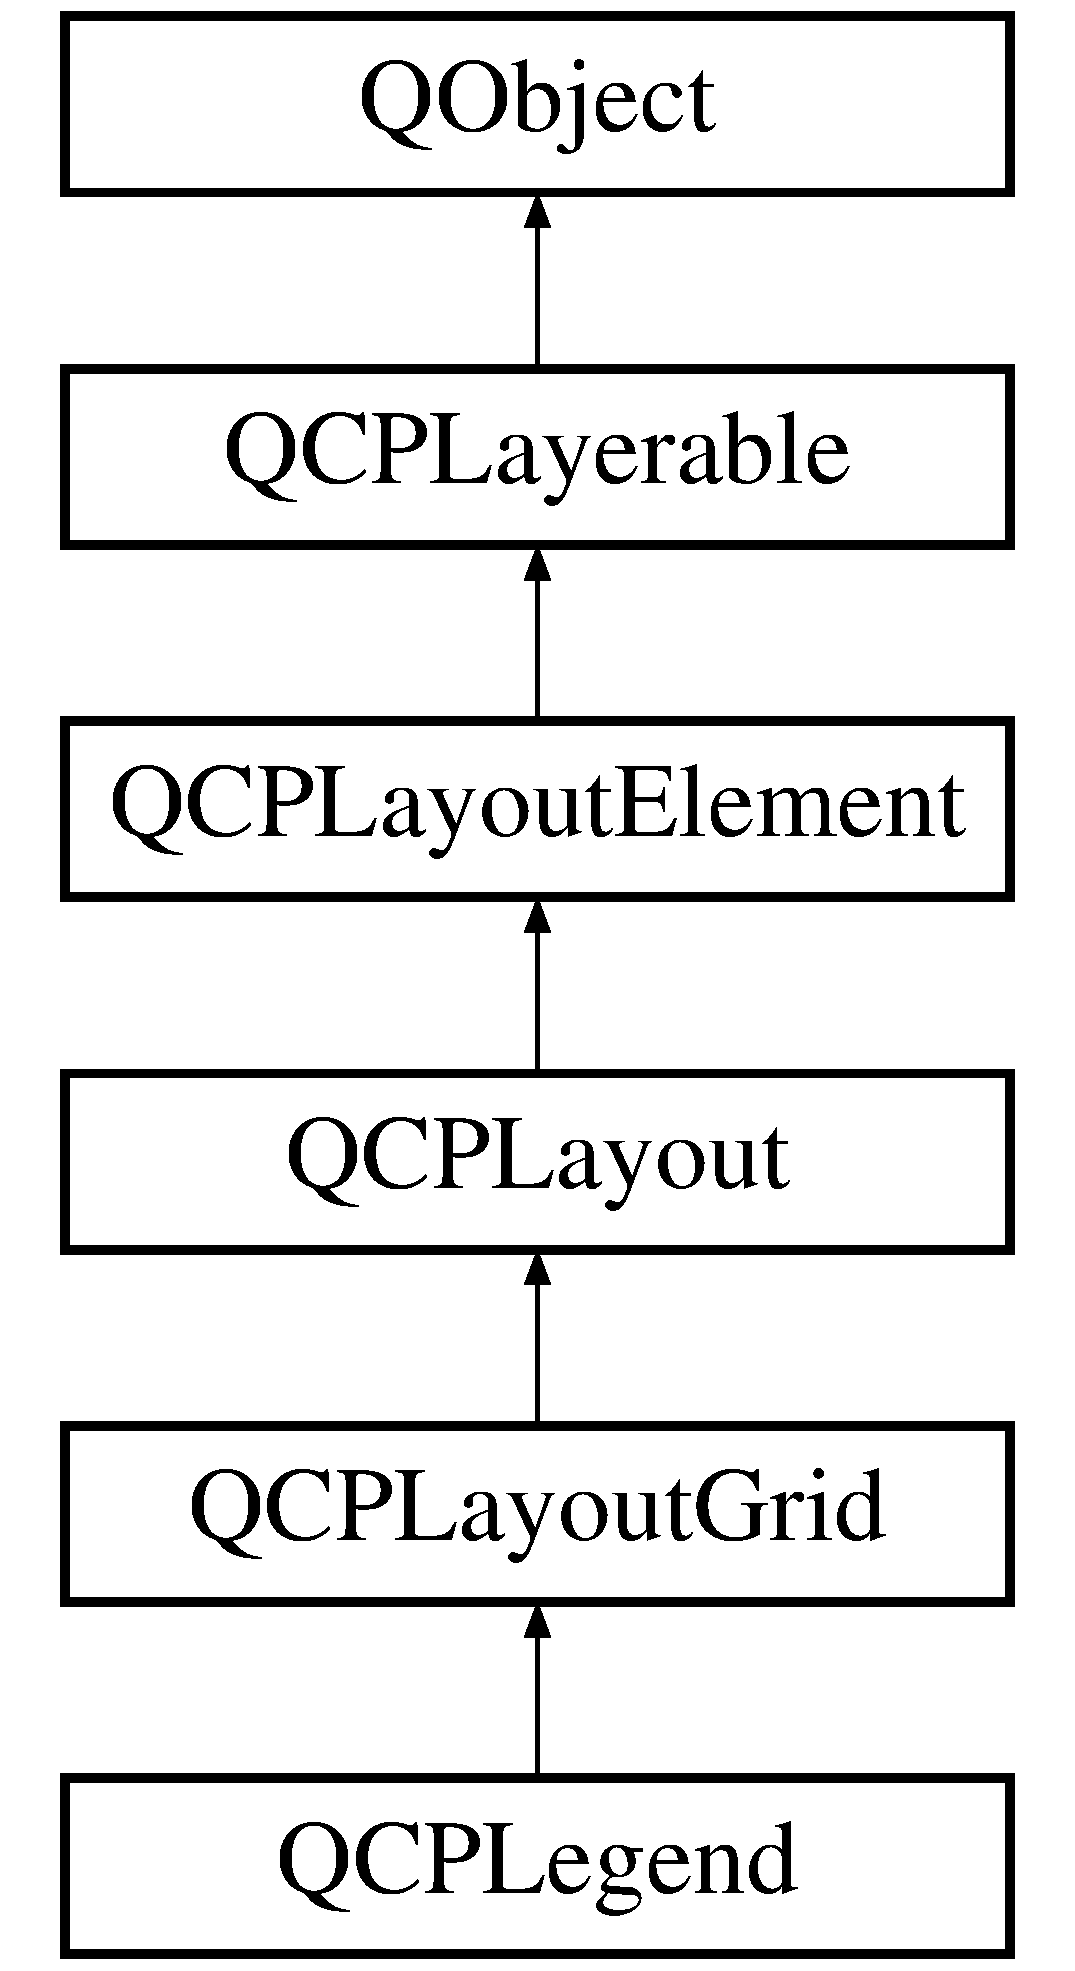
\includegraphics[height=6.000000cm]{class_q_c_p_legend}
\end{center}
\end{figure}
\subsection*{Public Types}
\begin{DoxyCompactItemize}
\item 
enum \hyperlink{class_q_c_p_legend_a5404de8bc1e4a994ca4ae69e2c7072f1}{Selectable\+Part} \{ \hyperlink{class_q_c_p_legend_a5404de8bc1e4a994ca4ae69e2c7072f1a378201c07d500af7126e3ec91652eed7}{sp\+None} = 0x000, 
\hyperlink{class_q_c_p_legend_a5404de8bc1e4a994ca4ae69e2c7072f1a0fa4758962a46fa1dc9da818abae23c4}{sp\+Legend\+Box} = 0x001, 
\hyperlink{class_q_c_p_legend_a5404de8bc1e4a994ca4ae69e2c7072f1a768bfb95f323db4c66473375032c0af7}{sp\+Items} = 0x002
 \}
\end{DoxyCompactItemize}
\subsection*{Signals}
\begin{DoxyCompactItemize}
\item 
void \hyperlink{class_q_c_p_legend_a82c88464edac07a9eefaf3906268df3b}{selection\+Changed} (Q\+C\+P\+Legend\+::\+Selectable\+Parts parts)
\item 
\hypertarget{class_q_c_p_legend_a8a77300fd0976d6bdd8000f4e8d114b8}{}\label{class_q_c_p_legend_a8a77300fd0976d6bdd8000f4e8d114b8} 
void {\bfseries selectable\+Changed} (Q\+C\+P\+Legend\+::\+Selectable\+Parts parts)
\end{DoxyCompactItemize}
\subsection*{Public Member Functions}
\begin{DoxyCompactItemize}
\item 
\hyperlink{class_q_c_p_legend_a0001a456989bd07ea378883651fabd72}{Q\+C\+P\+Legend} ()
\item 
\hypertarget{class_q_c_p_legend_a844b709a5632313416655f931c8e5631}{}\label{class_q_c_p_legend_a844b709a5632313416655f931c8e5631} 
Q\+Pen {\bfseries border\+Pen} () const
\item 
\hypertarget{class_q_c_p_legend_aaddafd5cbe9175512311350bb3b563e6}{}\label{class_q_c_p_legend_aaddafd5cbe9175512311350bb3b563e6} 
Q\+Brush {\bfseries brush} () const
\item 
\hypertarget{class_q_c_p_legend_ae240104de3c3a4cfc0834dbaffa07ac9}{}\label{class_q_c_p_legend_ae240104de3c3a4cfc0834dbaffa07ac9} 
Q\+Font {\bfseries font} () const
\item 
\hypertarget{class_q_c_p_legend_aa96d8f1a183ec2be8c0461c0abebd6db}{}\label{class_q_c_p_legend_aa96d8f1a183ec2be8c0461c0abebd6db} 
Q\+Color {\bfseries text\+Color} () const
\item 
\hypertarget{class_q_c_p_legend_ae4f17a186558c82d2ba269f6e7164dda}{}\label{class_q_c_p_legend_ae4f17a186558c82d2ba269f6e7164dda} 
Q\+Size {\bfseries icon\+Size} () const
\item 
\hypertarget{class_q_c_p_legend_a19668bb7f8fafe20d367cebf96269eaf}{}\label{class_q_c_p_legend_a19668bb7f8fafe20d367cebf96269eaf} 
int {\bfseries icon\+Text\+Padding} () const
\item 
\hypertarget{class_q_c_p_legend_a5b91d2ea68a4dd20238f660b80cd9945}{}\label{class_q_c_p_legend_a5b91d2ea68a4dd20238f660b80cd9945} 
Q\+Pen {\bfseries icon\+Border\+Pen} () const
\item 
\hypertarget{class_q_c_p_legend_ad091ff5e11edbe0adecba81c35522ac7}{}\label{class_q_c_p_legend_ad091ff5e11edbe0adecba81c35522ac7} 
Selectable\+Parts {\bfseries selectable\+Parts} () const
\item 
\hypertarget{class_q_c_p_legend_a3efbf879f6936ec337690985e567dc6f}{}\label{class_q_c_p_legend_a3efbf879f6936ec337690985e567dc6f} 
Selectable\+Parts {\bfseries selected\+Parts} () const
\item 
\hypertarget{class_q_c_p_legend_add8204bf083c82cc5def29093501a017}{}\label{class_q_c_p_legend_add8204bf083c82cc5def29093501a017} 
Q\+Pen {\bfseries selected\+Border\+Pen} () const
\item 
\hypertarget{class_q_c_p_legend_ad8eb320ca3a25928982a65163e8f883b}{}\label{class_q_c_p_legend_ad8eb320ca3a25928982a65163e8f883b} 
Q\+Pen {\bfseries selected\+Icon\+Border\+Pen} () const
\item 
\hypertarget{class_q_c_p_legend_a77dfa9340f68ca195f1817a93db09757}{}\label{class_q_c_p_legend_a77dfa9340f68ca195f1817a93db09757} 
Q\+Brush {\bfseries selected\+Brush} () const
\item 
\hypertarget{class_q_c_p_legend_a483ffd35d64710a165da87b9d9f11110}{}\label{class_q_c_p_legend_a483ffd35d64710a165da87b9d9f11110} 
Q\+Font {\bfseries selected\+Font} () const
\item 
\hypertarget{class_q_c_p_legend_ab9b469b27787bfb2ce6c8978a31821af}{}\label{class_q_c_p_legend_ab9b469b27787bfb2ce6c8978a31821af} 
Q\+Color {\bfseries selected\+Text\+Color} () const
\item 
void \hyperlink{class_q_c_p_legend_a866a9e3f5267de7430a6c7f26a61db9f}{set\+Border\+Pen} (const Q\+Pen \&pen)
\item 
void \hyperlink{class_q_c_p_legend_a497bbcd38baa3598c08e2b3f48103f23}{set\+Brush} (const Q\+Brush \&brush)
\item 
void \hyperlink{class_q_c_p_legend_aa4cda8499e3cb0f3be415edc02984c73}{set\+Font} (const Q\+Font \&font)
\item 
void \hyperlink{class_q_c_p_legend_ae1eb239ff4a4632fe1b6c3e668d845c6}{set\+Text\+Color} (const Q\+Color \&color)
\item 
void \hyperlink{class_q_c_p_legend_a8b0740cce488bf7010da6beda6898984}{set\+Icon\+Size} (const Q\+Size \&size)
\item 
void \hyperlink{class_q_c_p_legend_a96b1a37fd4ee6a9778e6e54fe56ab6c2}{set\+Icon\+Size} (int width, int height)
\item 
void \hyperlink{class_q_c_p_legend_a62973bd69d5155e8ea3141366e8968f6}{set\+Icon\+Text\+Padding} (int padding)
\item 
void \hyperlink{class_q_c_p_legend_a2f2c93d18a651f4ff294bb3f026f49b8}{set\+Icon\+Border\+Pen} (const Q\+Pen \&pen)
\item 
Q\+\_\+\+S\+L\+OT void \hyperlink{class_q_c_p_legend_a9ce60aa8bbd89f62ae4fa83ac6c60110}{set\+Selectable\+Parts} (const Selectable\+Parts \&selectable\+Parts)
\item 
Q\+\_\+\+S\+L\+OT void \hyperlink{class_q_c_p_legend_a2aee309bb5c2a794b1987f3fc97f8ad8}{set\+Selected\+Parts} (const Selectable\+Parts \&selected\+Parts)
\item 
void \hyperlink{class_q_c_p_legend_a2c35d262953a25d96b6112653fbefc88}{set\+Selected\+Border\+Pen} (const Q\+Pen \&pen)
\item 
void \hyperlink{class_q_c_p_legend_ade93aabe9bcccaf9cf46cec22c658027}{set\+Selected\+Icon\+Border\+Pen} (const Q\+Pen \&pen)
\item 
void \hyperlink{class_q_c_p_legend_a875227f3219c9799464631dec5e8f1bd}{set\+Selected\+Brush} (const Q\+Brush \&brush)
\item 
void \hyperlink{class_q_c_p_legend_ab580a01c3c0a239374ed66c29edf5ad2}{set\+Selected\+Font} (const Q\+Font \&font)
\item 
void \hyperlink{class_q_c_p_legend_a7674dfc7a1f30e1abd1018c0ed45e0bc}{set\+Selected\+Text\+Color} (const Q\+Color \&color)
\item 
virtual double \hyperlink{class_q_c_p_legend_acd7be544c81324e391cfa6be9c413c01}{select\+Test} (const Q\+PointF \&pos, bool only\+Selectable, Q\+Variant $\ast$details=0) const
\item 
\hyperlink{class_q_c_p_abstract_legend_item}{Q\+C\+P\+Abstract\+Legend\+Item} $\ast$ \hyperlink{class_q_c_p_legend_acfe9694c45104a3359d3806ed366fcf7}{item} (int index) const
\item 
\hyperlink{class_q_c_p_plottable_legend_item}{Q\+C\+P\+Plottable\+Legend\+Item} $\ast$ \hyperlink{class_q_c_p_legend_a91e790002d8bf15a20628a8e8841e397}{item\+With\+Plottable} (const \hyperlink{class_q_c_p_abstract_plottable}{Q\+C\+P\+Abstract\+Plottable} $\ast$plottable) const
\item 
int \hyperlink{class_q_c_p_legend_a57ab86ab8b2a3762d4c1455eb5452c88}{item\+Count} () const
\item 
bool \hyperlink{class_q_c_p_legend_ad0f698e33db454a6c103b5206740e599}{has\+Item} (\hyperlink{class_q_c_p_abstract_legend_item}{Q\+C\+P\+Abstract\+Legend\+Item} $\ast$\hyperlink{class_q_c_p_legend_acfe9694c45104a3359d3806ed366fcf7}{item}) const
\item 
bool \hyperlink{class_q_c_p_legend_a4b90a442af871582df85c2bc13f91e88}{has\+Item\+With\+Plottable} (const \hyperlink{class_q_c_p_abstract_plottable}{Q\+C\+P\+Abstract\+Plottable} $\ast$plottable) const
\item 
bool \hyperlink{class_q_c_p_legend_a3ab274de52d2951faea45a6d975e6b3f}{add\+Item} (\hyperlink{class_q_c_p_abstract_legend_item}{Q\+C\+P\+Abstract\+Legend\+Item} $\ast$\hyperlink{class_q_c_p_legend_acfe9694c45104a3359d3806ed366fcf7}{item})
\item 
bool \hyperlink{class_q_c_p_legend_ac91595c3eaa746fe6321d2eb952c63bb}{remove\+Item} (int index)
\item 
bool \hyperlink{class_q_c_p_legend_a2aea4ec6da2d454dd0b241a254d65082}{remove\+Item} (\hyperlink{class_q_c_p_abstract_legend_item}{Q\+C\+P\+Abstract\+Legend\+Item} $\ast$\hyperlink{class_q_c_p_legend_acfe9694c45104a3359d3806ed366fcf7}{item})
\item 
void \hyperlink{class_q_c_p_legend_a24795c7250eb5214fcea16b7217b4dfb}{clear\+Items} ()
\item 
Q\+List$<$ \hyperlink{class_q_c_p_abstract_legend_item}{Q\+C\+P\+Abstract\+Legend\+Item} $\ast$ $>$ \hyperlink{class_q_c_p_legend_ac7d9e567d5c551e09cd9bcc4306c5532}{selected\+Items} () const
\end{DoxyCompactItemize}
\subsection*{Protected Member Functions}
\begin{DoxyCompactItemize}
\item 
\hypertarget{class_q_c_p_legend_a4d552c63d82742d77fb7f177bae7b1ba}{}\label{class_q_c_p_legend_a4d552c63d82742d77fb7f177bae7b1ba} 
virtual void {\bfseries parent\+Plot\+Initialized} (\hyperlink{class_q_custom_plot}{Q\+Custom\+Plot} $\ast$parent\+Plot)
\item 
\hypertarget{class_q_c_p_legend_a8e11032dd41db9e53fd3ab0c3c813202}{}\label{class_q_c_p_legend_a8e11032dd41db9e53fd3ab0c3c813202} 
virtual \hyperlink{namespace_q_c_p_a2ad6bb6281c7c2d593d4277b44c2b037}{Q\+C\+P\+::\+Interaction} {\bfseries selection\+Category} () const
\item 
\hypertarget{class_q_c_p_legend_a1aea4fc7cdde130a58d0d225440cdbbb}{}\label{class_q_c_p_legend_a1aea4fc7cdde130a58d0d225440cdbbb} 
virtual void {\bfseries apply\+Default\+Antialiasing\+Hint} (\hyperlink{class_q_c_p_painter}{Q\+C\+P\+Painter} $\ast$painter) const
\item 
\hypertarget{class_q_c_p_legend_a4462151bf875ca85fa3815457c683fdc}{}\label{class_q_c_p_legend_a4462151bf875ca85fa3815457c683fdc} 
virtual void {\bfseries draw} (\hyperlink{class_q_c_p_painter}{Q\+C\+P\+Painter} $\ast$painter)
\item 
\hypertarget{class_q_c_p_legend_af93bf87dc5c383a9d2ada80b35f3a1a5}{}\label{class_q_c_p_legend_af93bf87dc5c383a9d2ada80b35f3a1a5} 
virtual void {\bfseries select\+Event} (Q\+Mouse\+Event $\ast$event, bool additive, const Q\+Variant \&details, bool $\ast$selection\+State\+Changed)
\item 
\hypertarget{class_q_c_p_legend_a5208ead4331c9b0440f768f059777c58}{}\label{class_q_c_p_legend_a5208ead4331c9b0440f768f059777c58} 
virtual void {\bfseries deselect\+Event} (bool $\ast$selection\+State\+Changed)
\item 
\hypertarget{class_q_c_p_legend_a1cf9df6f2130c5ad842dc92188ab6bd7}{}\label{class_q_c_p_legend_a1cf9df6f2130c5ad842dc92188ab6bd7} 
Q\+Pen {\bfseries get\+Border\+Pen} () const
\item 
\hypertarget{class_q_c_p_legend_ab1438d5d67304cdda3b9339da580d6bc}{}\label{class_q_c_p_legend_ab1438d5d67304cdda3b9339da580d6bc} 
Q\+Brush {\bfseries get\+Brush} () const
\end{DoxyCompactItemize}
\subsection*{Protected Attributes}
\begin{DoxyCompactItemize}
\item 
\hypertarget{class_q_c_p_legend_a52ab8342a382456131d567f962d7f9d0}{}\label{class_q_c_p_legend_a52ab8342a382456131d567f962d7f9d0} 
Q\+Pen {\bfseries m\+Border\+Pen}
\item 
\hypertarget{class_q_c_p_legend_a773ae518c3149fcabff4a2906fdacbc4}{}\label{class_q_c_p_legend_a773ae518c3149fcabff4a2906fdacbc4} 
Q\+Pen {\bfseries m\+Icon\+Border\+Pen}
\item 
\hypertarget{class_q_c_p_legend_a9bd7cd05a9a485e06eda513a348baf80}{}\label{class_q_c_p_legend_a9bd7cd05a9a485e06eda513a348baf80} 
Q\+Brush {\bfseries m\+Brush}
\item 
\hypertarget{class_q_c_p_legend_a56ffacb184a99eefe09a0c7181d0713d}{}\label{class_q_c_p_legend_a56ffacb184a99eefe09a0c7181d0713d} 
Q\+Font {\bfseries m\+Font}
\item 
\hypertarget{class_q_c_p_legend_a478b2d809a7390e9ff8f8bb70d6bd9fe}{}\label{class_q_c_p_legend_a478b2d809a7390e9ff8f8bb70d6bd9fe} 
Q\+Color {\bfseries m\+Text\+Color}
\item 
\hypertarget{class_q_c_p_legend_a39b972aae6c6a3fa5aa73313ab7a5765}{}\label{class_q_c_p_legend_a39b972aae6c6a3fa5aa73313ab7a5765} 
Q\+Size {\bfseries m\+Icon\+Size}
\item 
\hypertarget{class_q_c_p_legend_a8abf8843864ee9afc3f54f906c062240}{}\label{class_q_c_p_legend_a8abf8843864ee9afc3f54f906c062240} 
int {\bfseries m\+Icon\+Text\+Padding}
\item 
\hypertarget{class_q_c_p_legend_a917a34dd2856baafd8d56852d94d00e2}{}\label{class_q_c_p_legend_a917a34dd2856baafd8d56852d94d00e2} 
Selectable\+Parts {\bfseries m\+Selected\+Parts}
\item 
\hypertarget{class_q_c_p_legend_a179b4d5c1bea723b76e402ff48f0d7fb}{}\label{class_q_c_p_legend_a179b4d5c1bea723b76e402ff48f0d7fb} 
Selectable\+Parts {\bfseries m\+Selectable\+Parts}
\item 
\hypertarget{class_q_c_p_legend_a62906c996906ae23e9f724b6ac1f7334}{}\label{class_q_c_p_legend_a62906c996906ae23e9f724b6ac1f7334} 
Q\+Pen {\bfseries m\+Selected\+Border\+Pen}
\item 
\hypertarget{class_q_c_p_legend_a7429ac0e64c7b90b649b4d8f4cc5fa55}{}\label{class_q_c_p_legend_a7429ac0e64c7b90b649b4d8f4cc5fa55} 
Q\+Pen {\bfseries m\+Selected\+Icon\+Border\+Pen}
\item 
\hypertarget{class_q_c_p_legend_ab3c7567c86d4784b1e48f76a84b3a1e2}{}\label{class_q_c_p_legend_ab3c7567c86d4784b1e48f76a84b3a1e2} 
Q\+Brush {\bfseries m\+Selected\+Brush}
\item 
\hypertarget{class_q_c_p_legend_a86ce8f6c20a2f51a48eaf3c24ce16805}{}\label{class_q_c_p_legend_a86ce8f6c20a2f51a48eaf3c24ce16805} 
Q\+Font {\bfseries m\+Selected\+Font}
\item 
\hypertarget{class_q_c_p_legend_a6c25c8796c6e73e983aae6024965f2be}{}\label{class_q_c_p_legend_a6c25c8796c6e73e983aae6024965f2be} 
Q\+Color {\bfseries m\+Selected\+Text\+Color}
\end{DoxyCompactItemize}
\subsection*{Friends}
\begin{DoxyCompactItemize}
\item 
\hypertarget{class_q_c_p_legend_a1cdf9df76adcfae45261690aa0ca2198}{}\label{class_q_c_p_legend_a1cdf9df76adcfae45261690aa0ca2198} 
class {\bfseries Q\+Custom\+Plot}
\item 
\hypertarget{class_q_c_p_legend_a8a375e31e42c68de049fcf0fd35db5b0}{}\label{class_q_c_p_legend_a8a375e31e42c68de049fcf0fd35db5b0} 
class {\bfseries Q\+C\+P\+Abstract\+Legend\+Item}
\end{DoxyCompactItemize}


\subsection{Detailed Description}
Manages a legend inside a \hyperlink{class_q_custom_plot}{Q\+Custom\+Plot}. 

A legend is a small box somewhere in the plot which lists plottables with their name and icon.

Normally, the legend is populated by calling \hyperlink{class_q_c_p_abstract_plottable_a70f8cabfd808f7d5204b9f18c45c13f5}{Q\+C\+P\+Abstract\+Plottable\+::add\+To\+Legend}. The respective legend item can be removed with \hyperlink{class_q_c_p_abstract_plottable_ac95fb2604d9106d0852ad9ceb326fe8c}{Q\+C\+P\+Abstract\+Plottable\+::remove\+From\+Legend}. However, \hyperlink{class_q_c_p_legend}{Q\+C\+P\+Legend} also offers an interface to add and manipulate legend items directly\+: \hyperlink{class_q_c_p_legend_acfe9694c45104a3359d3806ed366fcf7}{item}, \hyperlink{class_q_c_p_legend_a91e790002d8bf15a20628a8e8841e397}{item\+With\+Plottable}, \hyperlink{class_q_c_p_legend_a57ab86ab8b2a3762d4c1455eb5452c88}{item\+Count}, \hyperlink{class_q_c_p_legend_a3ab274de52d2951faea45a6d975e6b3f}{add\+Item}, \hyperlink{class_q_c_p_legend_ac91595c3eaa746fe6321d2eb952c63bb}{remove\+Item}, etc.

The \hyperlink{class_q_c_p_legend}{Q\+C\+P\+Legend} derives from \hyperlink{class_q_c_p_layout_grid}{Q\+C\+P\+Layout\+Grid} and as such can be placed in any position a \hyperlink{class_q_c_p_layout_element}{Q\+C\+P\+Layout\+Element} may be positioned. The legend items are themselves Q\+C\+P\+Layout\+Elements which are placed in the grid layout of the legend. \hyperlink{class_q_c_p_legend}{Q\+C\+P\+Legend} only adds an interface specialized for handling child elements of type \hyperlink{class_q_c_p_abstract_legend_item}{Q\+C\+P\+Abstract\+Legend\+Item}, as mentioned above. In principle, any other layout elements may also be added to a legend via the normal \hyperlink{class_q_c_p_layout_grid}{Q\+C\+P\+Layout\+Grid} interface. However, the Q\+C\+P\+Abstract\+Legend\+Item-\/\+Interface will ignore those elements (e.\+g. \hyperlink{class_q_c_p_legend_a57ab86ab8b2a3762d4c1455eb5452c88}{item\+Count} will only return the number of items with Q\+C\+P\+Abstract\+Legend\+Items type).

By default, every \hyperlink{class_q_custom_plot}{Q\+Custom\+Plot} has one legend (\hyperlink{class_q_custom_plot_a4eadcd237dc6a09938b68b16877fa6af}{Q\+Custom\+Plot\+::legend}) which is placed in the inset layout of the main axis rect (\hyperlink{class_q_c_p_axis_rect_a949f803466619924c7018df4b511ae10}{Q\+C\+P\+Axis\+Rect\+::inset\+Layout}). To move the legend to another position inside the axis rect, use the methods of the \hyperlink{class_q_c_p_layout_inset}{Q\+C\+P\+Layout\+Inset}. To move the legend outside of the axis rect, place it anywhere else with the Q\+C\+P\+Layout/\+Q\+C\+P\+Layout\+Element interface. 

\subsection{Member Enumeration Documentation}
\hypertarget{class_q_c_p_legend_a5404de8bc1e4a994ca4ae69e2c7072f1}{}\label{class_q_c_p_legend_a5404de8bc1e4a994ca4ae69e2c7072f1} 
\index{Q\+C\+P\+Legend@{Q\+C\+P\+Legend}!Selectable\+Part@{Selectable\+Part}}
\index{Selectable\+Part@{Selectable\+Part}!Q\+C\+P\+Legend@{Q\+C\+P\+Legend}}
\subsubsection{\texorpdfstring{Selectable\+Part}{SelectablePart}}
{\footnotesize\ttfamily enum \hyperlink{class_q_c_p_legend_a5404de8bc1e4a994ca4ae69e2c7072f1}{Q\+C\+P\+Legend\+::\+Selectable\+Part}}

Defines the selectable parts of a legend

\begin{DoxySeeAlso}{See also}
\hyperlink{class_q_c_p_legend_a2aee309bb5c2a794b1987f3fc97f8ad8}{set\+Selected\+Parts}, \hyperlink{class_q_c_p_legend_a9ce60aa8bbd89f62ae4fa83ac6c60110}{set\+Selectable\+Parts} 
\end{DoxySeeAlso}
\begin{DoxyEnumFields}{Enumerator}
\raisebox{\heightof{T}}[0pt][0pt]{\index{sp\+None@{sp\+None}!Q\+C\+P\+Legend@{Q\+C\+P\+Legend}}\index{Q\+C\+P\+Legend@{Q\+C\+P\+Legend}!sp\+None@{sp\+None}}}\hypertarget{class_q_c_p_legend_a5404de8bc1e4a994ca4ae69e2c7072f1a378201c07d500af7126e3ec91652eed7}{}\label{class_q_c_p_legend_a5404de8bc1e4a994ca4ae69e2c7072f1a378201c07d500af7126e3ec91652eed7} 
sp\+None&{\ttfamily 0x000} None \\
\hline

\raisebox{\heightof{T}}[0pt][0pt]{\index{sp\+Legend\+Box@{sp\+Legend\+Box}!Q\+C\+P\+Legend@{Q\+C\+P\+Legend}}\index{Q\+C\+P\+Legend@{Q\+C\+P\+Legend}!sp\+Legend\+Box@{sp\+Legend\+Box}}}\hypertarget{class_q_c_p_legend_a5404de8bc1e4a994ca4ae69e2c7072f1a0fa4758962a46fa1dc9da818abae23c4}{}\label{class_q_c_p_legend_a5404de8bc1e4a994ca4ae69e2c7072f1a0fa4758962a46fa1dc9da818abae23c4} 
sp\+Legend\+Box&{\ttfamily 0x001} The legend box (frame) \\
\hline

\raisebox{\heightof{T}}[0pt][0pt]{\index{sp\+Items@{sp\+Items}!Q\+C\+P\+Legend@{Q\+C\+P\+Legend}}\index{Q\+C\+P\+Legend@{Q\+C\+P\+Legend}!sp\+Items@{sp\+Items}}}\hypertarget{class_q_c_p_legend_a5404de8bc1e4a994ca4ae69e2c7072f1a768bfb95f323db4c66473375032c0af7}{}\label{class_q_c_p_legend_a5404de8bc1e4a994ca4ae69e2c7072f1a768bfb95f323db4c66473375032c0af7} 
sp\+Items&{\ttfamily 0x002} Legend items individually (see \hyperlink{class_q_c_p_legend_ac7d9e567d5c551e09cd9bcc4306c5532}{selected\+Items}) \\
\hline

\end{DoxyEnumFields}


\subsection{Constructor \& Destructor Documentation}
\hypertarget{class_q_c_p_legend_a0001a456989bd07ea378883651fabd72}{}\label{class_q_c_p_legend_a0001a456989bd07ea378883651fabd72} 
\index{Q\+C\+P\+Legend@{Q\+C\+P\+Legend}!Q\+C\+P\+Legend@{Q\+C\+P\+Legend}}
\index{Q\+C\+P\+Legend@{Q\+C\+P\+Legend}!Q\+C\+P\+Legend@{Q\+C\+P\+Legend}}
\subsubsection{\texorpdfstring{Q\+C\+P\+Legend()}{QCPLegend()}}
{\footnotesize\ttfamily Q\+C\+P\+Legend\+::\+Q\+C\+P\+Legend (\begin{DoxyParamCaption}{ }\end{DoxyParamCaption})\hspace{0.3cm}{\ttfamily [explicit]}}

Constructs a new \hyperlink{class_q_c_p_legend}{Q\+C\+P\+Legend} instance with {\itshape parent\+Plot} as the containing plot and default values.

Note that by default, \hyperlink{class_q_custom_plot}{Q\+Custom\+Plot} already contains a legend ready to be used as \hyperlink{class_q_custom_plot_a4eadcd237dc6a09938b68b16877fa6af}{Q\+Custom\+Plot\+::legend} 

\subsection{Member Function Documentation}
\hypertarget{class_q_c_p_legend_a3ab274de52d2951faea45a6d975e6b3f}{}\label{class_q_c_p_legend_a3ab274de52d2951faea45a6d975e6b3f} 
\index{Q\+C\+P\+Legend@{Q\+C\+P\+Legend}!add\+Item@{add\+Item}}
\index{add\+Item@{add\+Item}!Q\+C\+P\+Legend@{Q\+C\+P\+Legend}}
\subsubsection{\texorpdfstring{add\+Item()}{addItem()}}
{\footnotesize\ttfamily bool Q\+C\+P\+Legend\+::add\+Item (\begin{DoxyParamCaption}\item[{\hyperlink{class_q_c_p_abstract_legend_item}{Q\+C\+P\+Abstract\+Legend\+Item} $\ast$}]{item }\end{DoxyParamCaption})}

Adds {\itshape item} to the legend, if it\textquotesingle{}s not present already.

Returns true on sucess, i.\+e. if the item wasn\textquotesingle{}t in the list already and has been successfuly added.

The legend takes ownership of the item. \hypertarget{class_q_c_p_legend_a24795c7250eb5214fcea16b7217b4dfb}{}\label{class_q_c_p_legend_a24795c7250eb5214fcea16b7217b4dfb} 
\index{Q\+C\+P\+Legend@{Q\+C\+P\+Legend}!clear\+Items@{clear\+Items}}
\index{clear\+Items@{clear\+Items}!Q\+C\+P\+Legend@{Q\+C\+P\+Legend}}
\subsubsection{\texorpdfstring{clear\+Items()}{clearItems()}}
{\footnotesize\ttfamily void Q\+C\+P\+Legend\+::clear\+Items (\begin{DoxyParamCaption}{ }\end{DoxyParamCaption})}

Removes all items from the legend. \hypertarget{class_q_c_p_legend_ad0f698e33db454a6c103b5206740e599}{}\label{class_q_c_p_legend_ad0f698e33db454a6c103b5206740e599} 
\index{Q\+C\+P\+Legend@{Q\+C\+P\+Legend}!has\+Item@{has\+Item}}
\index{has\+Item@{has\+Item}!Q\+C\+P\+Legend@{Q\+C\+P\+Legend}}
\subsubsection{\texorpdfstring{has\+Item()}{hasItem()}}
{\footnotesize\ttfamily bool Q\+C\+P\+Legend\+::has\+Item (\begin{DoxyParamCaption}\item[{\hyperlink{class_q_c_p_abstract_legend_item}{Q\+C\+P\+Abstract\+Legend\+Item} $\ast$}]{item }\end{DoxyParamCaption}) const}

Returns whether the legend contains {\itshape itm}. \hypertarget{class_q_c_p_legend_a4b90a442af871582df85c2bc13f91e88}{}\label{class_q_c_p_legend_a4b90a442af871582df85c2bc13f91e88} 
\index{Q\+C\+P\+Legend@{Q\+C\+P\+Legend}!has\+Item\+With\+Plottable@{has\+Item\+With\+Plottable}}
\index{has\+Item\+With\+Plottable@{has\+Item\+With\+Plottable}!Q\+C\+P\+Legend@{Q\+C\+P\+Legend}}
\subsubsection{\texorpdfstring{has\+Item\+With\+Plottable()}{hasItemWithPlottable()}}
{\footnotesize\ttfamily bool Q\+C\+P\+Legend\+::has\+Item\+With\+Plottable (\begin{DoxyParamCaption}\item[{const \hyperlink{class_q_c_p_abstract_plottable}{Q\+C\+P\+Abstract\+Plottable} $\ast$}]{plottable }\end{DoxyParamCaption}) const}

Returns whether the legend contains a \hyperlink{class_q_c_p_plottable_legend_item}{Q\+C\+P\+Plottable\+Legend\+Item} which is associated with {\itshape plottable} (e.\+g. a \hyperlink{class_q_c_p_graph}{Q\+C\+P\+Graph}$\ast$). If such an item isn\textquotesingle{}t in the legend, returns false.

\begin{DoxySeeAlso}{See also}
\hyperlink{class_q_c_p_legend_a91e790002d8bf15a20628a8e8841e397}{item\+With\+Plottable} 
\end{DoxySeeAlso}
\hypertarget{class_q_c_p_legend_acfe9694c45104a3359d3806ed366fcf7}{}\label{class_q_c_p_legend_acfe9694c45104a3359d3806ed366fcf7} 
\index{Q\+C\+P\+Legend@{Q\+C\+P\+Legend}!item@{item}}
\index{item@{item}!Q\+C\+P\+Legend@{Q\+C\+P\+Legend}}
\subsubsection{\texorpdfstring{item()}{item()}}
{\footnotesize\ttfamily \hyperlink{class_q_c_p_abstract_legend_item}{Q\+C\+P\+Abstract\+Legend\+Item} $\ast$ Q\+C\+P\+Legend\+::item (\begin{DoxyParamCaption}\item[{int}]{index }\end{DoxyParamCaption}) const}

Returns the item with index {\itshape i}.

\begin{DoxySeeAlso}{See also}
\hyperlink{class_q_c_p_legend_a57ab86ab8b2a3762d4c1455eb5452c88}{item\+Count} 
\end{DoxySeeAlso}
\hypertarget{class_q_c_p_legend_a57ab86ab8b2a3762d4c1455eb5452c88}{}\label{class_q_c_p_legend_a57ab86ab8b2a3762d4c1455eb5452c88} 
\index{Q\+C\+P\+Legend@{Q\+C\+P\+Legend}!item\+Count@{item\+Count}}
\index{item\+Count@{item\+Count}!Q\+C\+P\+Legend@{Q\+C\+P\+Legend}}
\subsubsection{\texorpdfstring{item\+Count()}{itemCount()}}
{\footnotesize\ttfamily int Q\+C\+P\+Legend\+::item\+Count (\begin{DoxyParamCaption}{ }\end{DoxyParamCaption}) const}

Returns the number of items currently in the legend. \begin{DoxySeeAlso}{See also}
\hyperlink{class_q_c_p_legend_acfe9694c45104a3359d3806ed366fcf7}{item} 
\end{DoxySeeAlso}
\hypertarget{class_q_c_p_legend_a91e790002d8bf15a20628a8e8841e397}{}\label{class_q_c_p_legend_a91e790002d8bf15a20628a8e8841e397} 
\index{Q\+C\+P\+Legend@{Q\+C\+P\+Legend}!item\+With\+Plottable@{item\+With\+Plottable}}
\index{item\+With\+Plottable@{item\+With\+Plottable}!Q\+C\+P\+Legend@{Q\+C\+P\+Legend}}
\subsubsection{\texorpdfstring{item\+With\+Plottable()}{itemWithPlottable()}}
{\footnotesize\ttfamily \hyperlink{class_q_c_p_plottable_legend_item}{Q\+C\+P\+Plottable\+Legend\+Item} $\ast$ Q\+C\+P\+Legend\+::item\+With\+Plottable (\begin{DoxyParamCaption}\item[{const \hyperlink{class_q_c_p_abstract_plottable}{Q\+C\+P\+Abstract\+Plottable} $\ast$}]{plottable }\end{DoxyParamCaption}) const}

Returns the \hyperlink{class_q_c_p_plottable_legend_item}{Q\+C\+P\+Plottable\+Legend\+Item} which is associated with {\itshape plottable} (e.\+g. a \hyperlink{class_q_c_p_graph}{Q\+C\+P\+Graph}$\ast$). If such an item isn\textquotesingle{}t in the legend, returns 0.

\begin{DoxySeeAlso}{See also}
\hyperlink{class_q_c_p_legend_a4b90a442af871582df85c2bc13f91e88}{has\+Item\+With\+Plottable} 
\end{DoxySeeAlso}
\hypertarget{class_q_c_p_legend_ac91595c3eaa746fe6321d2eb952c63bb}{}\label{class_q_c_p_legend_ac91595c3eaa746fe6321d2eb952c63bb} 
\index{Q\+C\+P\+Legend@{Q\+C\+P\+Legend}!remove\+Item@{remove\+Item}}
\index{remove\+Item@{remove\+Item}!Q\+C\+P\+Legend@{Q\+C\+P\+Legend}}
\subsubsection{\texorpdfstring{remove\+Item()}{removeItem()}\hspace{0.1cm}{\footnotesize\ttfamily [1/2]}}
{\footnotesize\ttfamily bool Q\+C\+P\+Legend\+::remove\+Item (\begin{DoxyParamCaption}\item[{int}]{index }\end{DoxyParamCaption})}

Removes the item with index {\itshape index} from the legend.

Returns true, if successful.

\begin{DoxySeeAlso}{See also}
\hyperlink{class_q_c_p_legend_a57ab86ab8b2a3762d4c1455eb5452c88}{item\+Count}, \hyperlink{class_q_c_p_legend_a24795c7250eb5214fcea16b7217b4dfb}{clear\+Items} 
\end{DoxySeeAlso}
\hypertarget{class_q_c_p_legend_a2aea4ec6da2d454dd0b241a254d65082}{}\label{class_q_c_p_legend_a2aea4ec6da2d454dd0b241a254d65082} 
\index{Q\+C\+P\+Legend@{Q\+C\+P\+Legend}!remove\+Item@{remove\+Item}}
\index{remove\+Item@{remove\+Item}!Q\+C\+P\+Legend@{Q\+C\+P\+Legend}}
\subsubsection{\texorpdfstring{remove\+Item()}{removeItem()}\hspace{0.1cm}{\footnotesize\ttfamily [2/2]}}
{\footnotesize\ttfamily bool Q\+C\+P\+Legend\+::remove\+Item (\begin{DoxyParamCaption}\item[{\hyperlink{class_q_c_p_abstract_legend_item}{Q\+C\+P\+Abstract\+Legend\+Item} $\ast$}]{item }\end{DoxyParamCaption})}

This is an overloaded member function, provided for convenience. It differs from the above function only in what argument(s) it accepts.

Removes {\itshape item} from the legend.

Returns true, if successful.

\begin{DoxySeeAlso}{See also}
\hyperlink{class_q_c_p_legend_a24795c7250eb5214fcea16b7217b4dfb}{clear\+Items} 
\end{DoxySeeAlso}
\hypertarget{class_q_c_p_legend_ac7d9e567d5c551e09cd9bcc4306c5532}{}\label{class_q_c_p_legend_ac7d9e567d5c551e09cd9bcc4306c5532} 
\index{Q\+C\+P\+Legend@{Q\+C\+P\+Legend}!selected\+Items@{selected\+Items}}
\index{selected\+Items@{selected\+Items}!Q\+C\+P\+Legend@{Q\+C\+P\+Legend}}
\subsubsection{\texorpdfstring{selected\+Items()}{selectedItems()}}
{\footnotesize\ttfamily Q\+List$<$ \hyperlink{class_q_c_p_abstract_legend_item}{Q\+C\+P\+Abstract\+Legend\+Item} $\ast$ $>$ Q\+C\+P\+Legend\+::selected\+Items (\begin{DoxyParamCaption}{ }\end{DoxyParamCaption}) const}

Returns the legend items that are currently selected. If no items are selected, the list is empty.

\begin{DoxySeeAlso}{See also}
\hyperlink{class_q_c_p_abstract_legend_item_a6eed93b0ab99cb3eabb043fb08179c2b}{Q\+C\+P\+Abstract\+Legend\+Item\+::set\+Selected}, set\+Selectable 
\end{DoxySeeAlso}
\hypertarget{class_q_c_p_legend_a82c88464edac07a9eefaf3906268df3b}{}\label{class_q_c_p_legend_a82c88464edac07a9eefaf3906268df3b} 
\index{Q\+C\+P\+Legend@{Q\+C\+P\+Legend}!selection\+Changed@{selection\+Changed}}
\index{selection\+Changed@{selection\+Changed}!Q\+C\+P\+Legend@{Q\+C\+P\+Legend}}
\subsubsection{\texorpdfstring{selection\+Changed}{selectionChanged}}
{\footnotesize\ttfamily void Q\+C\+P\+Legend\+::selection\+Changed (\begin{DoxyParamCaption}\item[{Q\+C\+P\+Legend\+::\+Selectable\+Parts}]{selection }\end{DoxyParamCaption})\hspace{0.3cm}{\ttfamily [signal]}}

This signal is emitted when the selection state of this legend has changed.

\begin{DoxySeeAlso}{See also}
\hyperlink{class_q_c_p_legend_a2aee309bb5c2a794b1987f3fc97f8ad8}{set\+Selected\+Parts}, \hyperlink{class_q_c_p_legend_a9ce60aa8bbd89f62ae4fa83ac6c60110}{set\+Selectable\+Parts} 
\end{DoxySeeAlso}
\hypertarget{class_q_c_p_legend_acd7be544c81324e391cfa6be9c413c01}{}\label{class_q_c_p_legend_acd7be544c81324e391cfa6be9c413c01} 
\index{Q\+C\+P\+Legend@{Q\+C\+P\+Legend}!select\+Test@{select\+Test}}
\index{select\+Test@{select\+Test}!Q\+C\+P\+Legend@{Q\+C\+P\+Legend}}
\subsubsection{\texorpdfstring{select\+Test()}{selectTest()}}
{\footnotesize\ttfamily double Q\+C\+P\+Legend\+::select\+Test (\begin{DoxyParamCaption}\item[{const Q\+PointF \&}]{pos,  }\item[{bool}]{only\+Selectable,  }\item[{Q\+Variant $\ast$}]{details = {\ttfamily 0} }\end{DoxyParamCaption}) const\hspace{0.3cm}{\ttfamily [virtual]}}

Layout elements are sensitive to events inside their outer rect. If {\itshape pos} is within the outer rect, this method returns a value corresponding to 0.\+99 times the parent plot\textquotesingle{}s selection tolerance. However, layout elements are not selectable by default. So if {\itshape only\+Selectable} is true, -\/1.\+0 is returned.

See \hyperlink{class_q_c_p_layerable_a04db8351fefd44cfdb77958e75c6288e}{Q\+C\+P\+Layerable\+::select\+Test} for a general explanation of this virtual method.

\hyperlink{class_q_c_p_layout_element}{Q\+C\+P\+Layout\+Element} subclasses may reimplement this method to provide more specific selection test behaviour. 

Reimplemented from \hyperlink{class_q_c_p_layout_element_a0b96ae0d7bcfa6e38188fcb1e73e143f}{Q\+C\+P\+Layout\+Element}.

\hypertarget{class_q_c_p_legend_a866a9e3f5267de7430a6c7f26a61db9f}{}\label{class_q_c_p_legend_a866a9e3f5267de7430a6c7f26a61db9f} 
\index{Q\+C\+P\+Legend@{Q\+C\+P\+Legend}!set\+Border\+Pen@{set\+Border\+Pen}}
\index{set\+Border\+Pen@{set\+Border\+Pen}!Q\+C\+P\+Legend@{Q\+C\+P\+Legend}}
\subsubsection{\texorpdfstring{set\+Border\+Pen()}{setBorderPen()}}
{\footnotesize\ttfamily void Q\+C\+P\+Legend\+::set\+Border\+Pen (\begin{DoxyParamCaption}\item[{const Q\+Pen \&}]{pen }\end{DoxyParamCaption})}

Sets the pen, the border of the entire legend is drawn with. \hypertarget{class_q_c_p_legend_a497bbcd38baa3598c08e2b3f48103f23}{}\label{class_q_c_p_legend_a497bbcd38baa3598c08e2b3f48103f23} 
\index{Q\+C\+P\+Legend@{Q\+C\+P\+Legend}!set\+Brush@{set\+Brush}}
\index{set\+Brush@{set\+Brush}!Q\+C\+P\+Legend@{Q\+C\+P\+Legend}}
\subsubsection{\texorpdfstring{set\+Brush()}{setBrush()}}
{\footnotesize\ttfamily void Q\+C\+P\+Legend\+::set\+Brush (\begin{DoxyParamCaption}\item[{const Q\+Brush \&}]{brush }\end{DoxyParamCaption})}

Sets the brush of the legend background. \hypertarget{class_q_c_p_legend_aa4cda8499e3cb0f3be415edc02984c73}{}\label{class_q_c_p_legend_aa4cda8499e3cb0f3be415edc02984c73} 
\index{Q\+C\+P\+Legend@{Q\+C\+P\+Legend}!set\+Font@{set\+Font}}
\index{set\+Font@{set\+Font}!Q\+C\+P\+Legend@{Q\+C\+P\+Legend}}
\subsubsection{\texorpdfstring{set\+Font()}{setFont()}}
{\footnotesize\ttfamily void Q\+C\+P\+Legend\+::set\+Font (\begin{DoxyParamCaption}\item[{const Q\+Font \&}]{font }\end{DoxyParamCaption})}

Sets the default font of legend text. Legend items that draw text (e.\+g. the name of a graph) will use this font by default. However, a different font can be specified on a per-\/item-\/basis by accessing the specific legend item.

This function will also set {\itshape font} on all already existing legend items.

\begin{DoxySeeAlso}{See also}
\hyperlink{class_q_c_p_abstract_legend_item_a409c53455d8112f71d70c0c43eb10265}{Q\+C\+P\+Abstract\+Legend\+Item\+::set\+Font} 
\end{DoxySeeAlso}
\hypertarget{class_q_c_p_legend_a2f2c93d18a651f4ff294bb3f026f49b8}{}\label{class_q_c_p_legend_a2f2c93d18a651f4ff294bb3f026f49b8} 
\index{Q\+C\+P\+Legend@{Q\+C\+P\+Legend}!set\+Icon\+Border\+Pen@{set\+Icon\+Border\+Pen}}
\index{set\+Icon\+Border\+Pen@{set\+Icon\+Border\+Pen}!Q\+C\+P\+Legend@{Q\+C\+P\+Legend}}
\subsubsection{\texorpdfstring{set\+Icon\+Border\+Pen()}{setIconBorderPen()}}
{\footnotesize\ttfamily void Q\+C\+P\+Legend\+::set\+Icon\+Border\+Pen (\begin{DoxyParamCaption}\item[{const Q\+Pen \&}]{pen }\end{DoxyParamCaption})}

Sets the pen used to draw a border around each legend icon. Legend items that draw an icon (e.\+g. a visual representation of the graph) will use this pen by default.

If no border is wanted, set this to {\itshape Qt\+::\+No\+Pen}. \hypertarget{class_q_c_p_legend_a8b0740cce488bf7010da6beda6898984}{}\label{class_q_c_p_legend_a8b0740cce488bf7010da6beda6898984} 
\index{Q\+C\+P\+Legend@{Q\+C\+P\+Legend}!set\+Icon\+Size@{set\+Icon\+Size}}
\index{set\+Icon\+Size@{set\+Icon\+Size}!Q\+C\+P\+Legend@{Q\+C\+P\+Legend}}
\subsubsection{\texorpdfstring{set\+Icon\+Size()}{setIconSize()}\hspace{0.1cm}{\footnotesize\ttfamily [1/2]}}
{\footnotesize\ttfamily void Q\+C\+P\+Legend\+::set\+Icon\+Size (\begin{DoxyParamCaption}\item[{const Q\+Size \&}]{size }\end{DoxyParamCaption})}

Sets the size of legend icons. Legend items that draw an icon (e.\+g. a visual representation of the graph) will use this size by default. \hypertarget{class_q_c_p_legend_a96b1a37fd4ee6a9778e6e54fe56ab6c2}{}\label{class_q_c_p_legend_a96b1a37fd4ee6a9778e6e54fe56ab6c2} 
\index{Q\+C\+P\+Legend@{Q\+C\+P\+Legend}!set\+Icon\+Size@{set\+Icon\+Size}}
\index{set\+Icon\+Size@{set\+Icon\+Size}!Q\+C\+P\+Legend@{Q\+C\+P\+Legend}}
\subsubsection{\texorpdfstring{set\+Icon\+Size()}{setIconSize()}\hspace{0.1cm}{\footnotesize\ttfamily [2/2]}}
{\footnotesize\ttfamily void Q\+C\+P\+Legend\+::set\+Icon\+Size (\begin{DoxyParamCaption}\item[{int}]{width,  }\item[{int}]{height }\end{DoxyParamCaption})}

This is an overloaded member function, provided for convenience. It differs from the above function only in what argument(s) it accepts. \hypertarget{class_q_c_p_legend_a62973bd69d5155e8ea3141366e8968f6}{}\label{class_q_c_p_legend_a62973bd69d5155e8ea3141366e8968f6} 
\index{Q\+C\+P\+Legend@{Q\+C\+P\+Legend}!set\+Icon\+Text\+Padding@{set\+Icon\+Text\+Padding}}
\index{set\+Icon\+Text\+Padding@{set\+Icon\+Text\+Padding}!Q\+C\+P\+Legend@{Q\+C\+P\+Legend}}
\subsubsection{\texorpdfstring{set\+Icon\+Text\+Padding()}{setIconTextPadding()}}
{\footnotesize\ttfamily void Q\+C\+P\+Legend\+::set\+Icon\+Text\+Padding (\begin{DoxyParamCaption}\item[{int}]{padding }\end{DoxyParamCaption})}

Sets the horizontal space in pixels between the legend icon and the text next to it. Legend items that draw an icon (e.\+g. a visual representation of the graph) and text (e.\+g. the name of the graph) will use this space by default. \hypertarget{class_q_c_p_legend_a9ce60aa8bbd89f62ae4fa83ac6c60110}{}\label{class_q_c_p_legend_a9ce60aa8bbd89f62ae4fa83ac6c60110} 
\index{Q\+C\+P\+Legend@{Q\+C\+P\+Legend}!set\+Selectable\+Parts@{set\+Selectable\+Parts}}
\index{set\+Selectable\+Parts@{set\+Selectable\+Parts}!Q\+C\+P\+Legend@{Q\+C\+P\+Legend}}
\subsubsection{\texorpdfstring{set\+Selectable\+Parts()}{setSelectableParts()}}
{\footnotesize\ttfamily void Q\+C\+P\+Legend\+::set\+Selectable\+Parts (\begin{DoxyParamCaption}\item[{const Selectable\+Parts \&}]{selectable }\end{DoxyParamCaption})}

Sets whether the user can (de-\/)select the parts in {\itshape selectable} by clicking on the \hyperlink{class_q_custom_plot}{Q\+Custom\+Plot} surface. (When \hyperlink{class_q_custom_plot_a5ee1e2f6ae27419deca53e75907c27e5}{Q\+Custom\+Plot\+::set\+Interactions} contains \hyperlink{namespace_q_c_p_a2ad6bb6281c7c2d593d4277b44c2b037a269c9af298e257d1108edec0432b5513}{Q\+C\+P\+::i\+Select\+Legend}.)

However, even when {\itshape selectable} is set to a value not allowing the selection of a specific part, it is still possible to set the selection of this part manually, by calling \hyperlink{class_q_c_p_legend_a2aee309bb5c2a794b1987f3fc97f8ad8}{set\+Selected\+Parts} directly.

\begin{DoxySeeAlso}{See also}
\hyperlink{class_q_c_p_legend_a5404de8bc1e4a994ca4ae69e2c7072f1}{Selectable\+Part}, \hyperlink{class_q_c_p_legend_a2aee309bb5c2a794b1987f3fc97f8ad8}{set\+Selected\+Parts} 
\end{DoxySeeAlso}
\hypertarget{class_q_c_p_legend_a2c35d262953a25d96b6112653fbefc88}{}\label{class_q_c_p_legend_a2c35d262953a25d96b6112653fbefc88} 
\index{Q\+C\+P\+Legend@{Q\+C\+P\+Legend}!set\+Selected\+Border\+Pen@{set\+Selected\+Border\+Pen}}
\index{set\+Selected\+Border\+Pen@{set\+Selected\+Border\+Pen}!Q\+C\+P\+Legend@{Q\+C\+P\+Legend}}
\subsubsection{\texorpdfstring{set\+Selected\+Border\+Pen()}{setSelectedBorderPen()}}
{\footnotesize\ttfamily void Q\+C\+P\+Legend\+::set\+Selected\+Border\+Pen (\begin{DoxyParamCaption}\item[{const Q\+Pen \&}]{pen }\end{DoxyParamCaption})}

When the legend box is selected, this pen is used to draw the border instead of the normal pen set via \hyperlink{class_q_c_p_legend_a866a9e3f5267de7430a6c7f26a61db9f}{set\+Border\+Pen}.

\begin{DoxySeeAlso}{See also}
\hyperlink{class_q_c_p_legend_a2aee309bb5c2a794b1987f3fc97f8ad8}{set\+Selected\+Parts}, \hyperlink{class_q_c_p_legend_a9ce60aa8bbd89f62ae4fa83ac6c60110}{set\+Selectable\+Parts}, \hyperlink{class_q_c_p_legend_a875227f3219c9799464631dec5e8f1bd}{set\+Selected\+Brush} 
\end{DoxySeeAlso}
\hypertarget{class_q_c_p_legend_a875227f3219c9799464631dec5e8f1bd}{}\label{class_q_c_p_legend_a875227f3219c9799464631dec5e8f1bd} 
\index{Q\+C\+P\+Legend@{Q\+C\+P\+Legend}!set\+Selected\+Brush@{set\+Selected\+Brush}}
\index{set\+Selected\+Brush@{set\+Selected\+Brush}!Q\+C\+P\+Legend@{Q\+C\+P\+Legend}}
\subsubsection{\texorpdfstring{set\+Selected\+Brush()}{setSelectedBrush()}}
{\footnotesize\ttfamily void Q\+C\+P\+Legend\+::set\+Selected\+Brush (\begin{DoxyParamCaption}\item[{const Q\+Brush \&}]{brush }\end{DoxyParamCaption})}

When the legend box is selected, this brush is used to draw the legend background instead of the normal brush set via \hyperlink{class_q_c_p_legend_a497bbcd38baa3598c08e2b3f48103f23}{set\+Brush}.

\begin{DoxySeeAlso}{See also}
\hyperlink{class_q_c_p_legend_a2aee309bb5c2a794b1987f3fc97f8ad8}{set\+Selected\+Parts}, \hyperlink{class_q_c_p_legend_a9ce60aa8bbd89f62ae4fa83ac6c60110}{set\+Selectable\+Parts}, \hyperlink{class_q_c_p_legend_a2c35d262953a25d96b6112653fbefc88}{set\+Selected\+Border\+Pen} 
\end{DoxySeeAlso}
\hypertarget{class_q_c_p_legend_ab580a01c3c0a239374ed66c29edf5ad2}{}\label{class_q_c_p_legend_ab580a01c3c0a239374ed66c29edf5ad2} 
\index{Q\+C\+P\+Legend@{Q\+C\+P\+Legend}!set\+Selected\+Font@{set\+Selected\+Font}}
\index{set\+Selected\+Font@{set\+Selected\+Font}!Q\+C\+P\+Legend@{Q\+C\+P\+Legend}}
\subsubsection{\texorpdfstring{set\+Selected\+Font()}{setSelectedFont()}}
{\footnotesize\ttfamily void Q\+C\+P\+Legend\+::set\+Selected\+Font (\begin{DoxyParamCaption}\item[{const Q\+Font \&}]{font }\end{DoxyParamCaption})}

Sets the default font that is used by legend items when they are selected.

This function will also set {\itshape font} on all already existing legend items.

\begin{DoxySeeAlso}{See also}
\hyperlink{class_q_c_p_legend_aa4cda8499e3cb0f3be415edc02984c73}{set\+Font}, \hyperlink{class_q_c_p_abstract_legend_item_a91db5aee48617a9d3206e61376807365}{Q\+C\+P\+Abstract\+Legend\+Item\+::set\+Selected\+Font} 
\end{DoxySeeAlso}
\hypertarget{class_q_c_p_legend_ade93aabe9bcccaf9cf46cec22c658027}{}\label{class_q_c_p_legend_ade93aabe9bcccaf9cf46cec22c658027} 
\index{Q\+C\+P\+Legend@{Q\+C\+P\+Legend}!set\+Selected\+Icon\+Border\+Pen@{set\+Selected\+Icon\+Border\+Pen}}
\index{set\+Selected\+Icon\+Border\+Pen@{set\+Selected\+Icon\+Border\+Pen}!Q\+C\+P\+Legend@{Q\+C\+P\+Legend}}
\subsubsection{\texorpdfstring{set\+Selected\+Icon\+Border\+Pen()}{setSelectedIconBorderPen()}}
{\footnotesize\ttfamily void Q\+C\+P\+Legend\+::set\+Selected\+Icon\+Border\+Pen (\begin{DoxyParamCaption}\item[{const Q\+Pen \&}]{pen }\end{DoxyParamCaption})}

Sets the pen legend items will use to draw their icon borders, when they are selected.

\begin{DoxySeeAlso}{See also}
\hyperlink{class_q_c_p_legend_a2aee309bb5c2a794b1987f3fc97f8ad8}{set\+Selected\+Parts}, \hyperlink{class_q_c_p_legend_a9ce60aa8bbd89f62ae4fa83ac6c60110}{set\+Selectable\+Parts}, \hyperlink{class_q_c_p_legend_ab580a01c3c0a239374ed66c29edf5ad2}{set\+Selected\+Font} 
\end{DoxySeeAlso}
\hypertarget{class_q_c_p_legend_a2aee309bb5c2a794b1987f3fc97f8ad8}{}\label{class_q_c_p_legend_a2aee309bb5c2a794b1987f3fc97f8ad8} 
\index{Q\+C\+P\+Legend@{Q\+C\+P\+Legend}!set\+Selected\+Parts@{set\+Selected\+Parts}}
\index{set\+Selected\+Parts@{set\+Selected\+Parts}!Q\+C\+P\+Legend@{Q\+C\+P\+Legend}}
\subsubsection{\texorpdfstring{set\+Selected\+Parts()}{setSelectedParts()}}
{\footnotesize\ttfamily void Q\+C\+P\+Legend\+::set\+Selected\+Parts (\begin{DoxyParamCaption}\item[{const Selectable\+Parts \&}]{selected }\end{DoxyParamCaption})}

Sets the selected state of the respective legend parts described by \hyperlink{class_q_c_p_legend_a5404de8bc1e4a994ca4ae69e2c7072f1}{Selectable\+Part}. When a part is selected, it uses a different pen/font and brush. If some legend items are selected and {\itshape selected} doesn\textquotesingle{}t contain \hyperlink{class_q_c_p_legend_a5404de8bc1e4a994ca4ae69e2c7072f1a768bfb95f323db4c66473375032c0af7}{sp\+Items}, those items become deselected.

The entire selection mechanism is handled automatically when \hyperlink{class_q_custom_plot_a5ee1e2f6ae27419deca53e75907c27e5}{Q\+Custom\+Plot\+::set\+Interactions} contains i\+Select\+Legend. You only need to call this function when you wish to change the selection state manually.

This function can change the selection state of a part even when \hyperlink{class_q_c_p_legend_a9ce60aa8bbd89f62ae4fa83ac6c60110}{set\+Selectable\+Parts} was set to a value that actually excludes the part.

emits the \hyperlink{class_q_c_p_legend_a82c88464edac07a9eefaf3906268df3b}{selection\+Changed} signal when {\itshape selected} is different from the previous selection state.

Note that it doesn\textquotesingle{}t make sense to set the selected state \hyperlink{class_q_c_p_legend_a5404de8bc1e4a994ca4ae69e2c7072f1a768bfb95f323db4c66473375032c0af7}{sp\+Items} here when it wasn\textquotesingle{}t set before, because there\textquotesingle{}s no way to specify which exact items to newly select. Do this by calling \hyperlink{class_q_c_p_abstract_legend_item_a6eed93b0ab99cb3eabb043fb08179c2b}{Q\+C\+P\+Abstract\+Legend\+Item\+::set\+Selected} directly on the legend item you wish to select.

\begin{DoxySeeAlso}{See also}
\hyperlink{class_q_c_p_legend_a5404de8bc1e4a994ca4ae69e2c7072f1}{Selectable\+Part}, \hyperlink{class_q_c_p_legend_a9ce60aa8bbd89f62ae4fa83ac6c60110}{set\+Selectable\+Parts}, \hyperlink{class_q_c_p_legend_acd7be544c81324e391cfa6be9c413c01}{select\+Test}, \hyperlink{class_q_c_p_legend_a2c35d262953a25d96b6112653fbefc88}{set\+Selected\+Border\+Pen}, \hyperlink{class_q_c_p_legend_ade93aabe9bcccaf9cf46cec22c658027}{set\+Selected\+Icon\+Border\+Pen}, \hyperlink{class_q_c_p_legend_a875227f3219c9799464631dec5e8f1bd}{set\+Selected\+Brush}, \hyperlink{class_q_c_p_legend_ab580a01c3c0a239374ed66c29edf5ad2}{set\+Selected\+Font} 
\end{DoxySeeAlso}
\hypertarget{class_q_c_p_legend_a7674dfc7a1f30e1abd1018c0ed45e0bc}{}\label{class_q_c_p_legend_a7674dfc7a1f30e1abd1018c0ed45e0bc} 
\index{Q\+C\+P\+Legend@{Q\+C\+P\+Legend}!set\+Selected\+Text\+Color@{set\+Selected\+Text\+Color}}
\index{set\+Selected\+Text\+Color@{set\+Selected\+Text\+Color}!Q\+C\+P\+Legend@{Q\+C\+P\+Legend}}
\subsubsection{\texorpdfstring{set\+Selected\+Text\+Color()}{setSelectedTextColor()}}
{\footnotesize\ttfamily void Q\+C\+P\+Legend\+::set\+Selected\+Text\+Color (\begin{DoxyParamCaption}\item[{const Q\+Color \&}]{color }\end{DoxyParamCaption})}

Sets the default text color that is used by legend items when they are selected.

This function will also set {\itshape color} on all already existing legend items.

\begin{DoxySeeAlso}{See also}
\hyperlink{class_q_c_p_legend_ae1eb239ff4a4632fe1b6c3e668d845c6}{set\+Text\+Color}, \hyperlink{class_q_c_p_abstract_legend_item_a4d01d008ee1a5bfe9905b0397a421936}{Q\+C\+P\+Abstract\+Legend\+Item\+::set\+Selected\+Text\+Color} 
\end{DoxySeeAlso}
\hypertarget{class_q_c_p_legend_ae1eb239ff4a4632fe1b6c3e668d845c6}{}\label{class_q_c_p_legend_ae1eb239ff4a4632fe1b6c3e668d845c6} 
\index{Q\+C\+P\+Legend@{Q\+C\+P\+Legend}!set\+Text\+Color@{set\+Text\+Color}}
\index{set\+Text\+Color@{set\+Text\+Color}!Q\+C\+P\+Legend@{Q\+C\+P\+Legend}}
\subsubsection{\texorpdfstring{set\+Text\+Color()}{setTextColor()}}
{\footnotesize\ttfamily void Q\+C\+P\+Legend\+::set\+Text\+Color (\begin{DoxyParamCaption}\item[{const Q\+Color \&}]{color }\end{DoxyParamCaption})}

Sets the default color of legend text. Legend items that draw text (e.\+g. the name of a graph) will use this color by default. However, a different colors can be specified on a per-\/item-\/basis by accessing the specific legend item.

This function will also set {\itshape color} on all already existing legend items.

\begin{DoxySeeAlso}{See also}
\hyperlink{class_q_c_p_abstract_legend_item_a6ebace6aaffaedcdab2d74e88acc2d1e}{Q\+C\+P\+Abstract\+Legend\+Item\+::set\+Text\+Color} 
\end{DoxySeeAlso}


The documentation for this class was generated from the following files\+:\begin{DoxyCompactItemize}
\item 
F\+E\+S\+S-\/\+G\+U\+I/\hyperlink{qcustomplot_8h}{qcustomplot.\+h}\item 
F\+E\+S\+S-\/\+G\+U\+I/\hyperlink{qcustomplot_8cpp}{qcustomplot.\+cpp}\end{DoxyCompactItemize}

\hypertarget{class_q_c_p_line_ending}{}\section{Q\+C\+P\+Line\+Ending Class Reference}
\label{class_q_c_p_line_ending}\index{Q\+C\+P\+Line\+Ending@{Q\+C\+P\+Line\+Ending}}


Handles the different ending decorations for line-\/like items.  


\subsection*{Public Types}
\begin{DoxyCompactItemize}
\item 
enum \hyperlink{class_q_c_p_line_ending_a5ef16e6876b4b74959c7261d8d4c2cd5}{Ending\+Style} \{ \newline
\hyperlink{class_q_c_p_line_ending_a5ef16e6876b4b74959c7261d8d4c2cd5aca12d500f50cd6871766801bac30fb03}{es\+None}, 
\hyperlink{class_q_c_p_line_ending_a5ef16e6876b4b74959c7261d8d4c2cd5a3d7dcea2f100671727c3417142154f8f}{es\+Flat\+Arrow}, 
\hyperlink{class_q_c_p_line_ending_a5ef16e6876b4b74959c7261d8d4c2cd5ab9964d0d03f812d1e79de15edbeb2cbf}{es\+Spike\+Arrow}, 
\hyperlink{class_q_c_p_line_ending_a5ef16e6876b4b74959c7261d8d4c2cd5a61f78ee8f375fb21cb9d250687bbcbd2}{es\+Line\+Arrow}, 
\newline
\hyperlink{class_q_c_p_line_ending_a5ef16e6876b4b74959c7261d8d4c2cd5ae5a3414916817258bcc6dddd605e8f5c}{es\+Disc}, 
\hyperlink{class_q_c_p_line_ending_a5ef16e6876b4b74959c7261d8d4c2cd5ae1836502fa43d8990bb62b2d493a140a}{es\+Square}, 
\hyperlink{class_q_c_p_line_ending_a5ef16e6876b4b74959c7261d8d4c2cd5a378fe5a8b768411b0bc1765210fe7200}{es\+Diamond}, 
\hyperlink{class_q_c_p_line_ending_a5ef16e6876b4b74959c7261d8d4c2cd5a2cf543bbca332df26d89bf779f50469f}{es\+Bar}, 
\newline
\hyperlink{class_q_c_p_line_ending_a5ef16e6876b4b74959c7261d8d4c2cd5a126c390f0c359fcd8df1fc5e38d26d5b}{es\+Half\+Bar}, 
\hyperlink{class_q_c_p_line_ending_a5ef16e6876b4b74959c7261d8d4c2cd5a2b2cc96e757ca9bcd91fb70221ed43ab}{es\+Skewed\+Bar}
 \}
\end{DoxyCompactItemize}
\subsection*{Public Member Functions}
\begin{DoxyCompactItemize}
\item 
\hyperlink{class_q_c_p_line_ending_af2eaf8123b000d97fbd11929c669f61b}{Q\+C\+P\+Line\+Ending} ()
\item 
\hyperlink{class_q_c_p_line_ending_abb2abc7542f0c7a3c081d878248896a4}{Q\+C\+P\+Line\+Ending} (\hyperlink{class_q_c_p_line_ending_a5ef16e6876b4b74959c7261d8d4c2cd5}{Ending\+Style} style, double width=8, double length=10, bool inverted=false)
\item 
\hypertarget{class_q_c_p_line_ending_a07e75aaac6c61322bf51af237c5778e3}{}\label{class_q_c_p_line_ending_a07e75aaac6c61322bf51af237c5778e3} 
\hyperlink{class_q_c_p_line_ending_a5ef16e6876b4b74959c7261d8d4c2cd5}{Ending\+Style} {\bfseries style} () const
\item 
\hypertarget{class_q_c_p_line_ending_ae6f1fb83c210da6ace35d629993287f3}{}\label{class_q_c_p_line_ending_ae6f1fb83c210da6ace35d629993287f3} 
double {\bfseries width} () const
\item 
\hypertarget{class_q_c_p_line_ending_aee9050a13fe115bd1b6794f9ad14cd72}{}\label{class_q_c_p_line_ending_aee9050a13fe115bd1b6794f9ad14cd72} 
double {\bfseries length} () const
\item 
\hypertarget{class_q_c_p_line_ending_a15a68706d298a0c9f94556f6b4db15ff}{}\label{class_q_c_p_line_ending_a15a68706d298a0c9f94556f6b4db15ff} 
bool {\bfseries inverted} () const
\item 
void \hyperlink{class_q_c_p_line_ending_a56953b9cb8ed1bed0f025c3935f16910}{set\+Style} (\hyperlink{class_q_c_p_line_ending_a5ef16e6876b4b74959c7261d8d4c2cd5}{Ending\+Style} style)
\item 
void \hyperlink{class_q_c_p_line_ending_a26dc020ea985a72cc25881ce2115e34e}{set\+Width} (double width)
\item 
void \hyperlink{class_q_c_p_line_ending_ae36fa01763751cd64b7f56c3507e935a}{set\+Length} (double length)
\item 
void \hyperlink{class_q_c_p_line_ending_a580e4e2360b35ebb8d68f3494aa2335d}{set\+Inverted} (bool inverted)
\item 
\hypertarget{class_q_c_p_line_ending_a14fe390ddd590864ac66a60ed5278df5}{}\label{class_q_c_p_line_ending_a14fe390ddd590864ac66a60ed5278df5} 
double {\bfseries bounding\+Distance} () const
\item 
double \hyperlink{class_q_c_p_line_ending_acacd24d386d459b282d3c57f16a5405d}{real\+Length} () const
\item 
\hypertarget{class_q_c_p_line_ending_a13321409a5570be5d58d99b67bc73cd5}{}\label{class_q_c_p_line_ending_a13321409a5570be5d58d99b67bc73cd5} 
void {\bfseries draw} (\hyperlink{class_q_c_p_painter}{Q\+C\+P\+Painter} $\ast$painter, const Q\+Vector2D \&pos, const Q\+Vector2D \&dir) const
\item 
\hypertarget{class_q_c_p_line_ending_a851ac38f3aeabb0d31ada41198ae1480}{}\label{class_q_c_p_line_ending_a851ac38f3aeabb0d31ada41198ae1480} 
void {\bfseries draw} (\hyperlink{class_q_c_p_painter}{Q\+C\+P\+Painter} $\ast$painter, const Q\+Vector2D \&pos, double angle) const
\end{DoxyCompactItemize}
\subsection*{Protected Attributes}
\begin{DoxyCompactItemize}
\item 
\hypertarget{class_q_c_p_line_ending_a4696fc9117b60f1ca7690fcd2ba56611}{}\label{class_q_c_p_line_ending_a4696fc9117b60f1ca7690fcd2ba56611} 
\hyperlink{class_q_c_p_line_ending_a5ef16e6876b4b74959c7261d8d4c2cd5}{Ending\+Style} {\bfseries m\+Style}
\item 
\hypertarget{class_q_c_p_line_ending_aca89d21341133c20dc6825c33a5eac48}{}\label{class_q_c_p_line_ending_aca89d21341133c20dc6825c33a5eac48} 
double {\bfseries m\+Width}
\item 
\hypertarget{class_q_c_p_line_ending_ae8e1e2566b96c05736cd92662dba8af8}{}\label{class_q_c_p_line_ending_ae8e1e2566b96c05736cd92662dba8af8} 
double {\bfseries m\+Length}
\item 
\hypertarget{class_q_c_p_line_ending_a91306fe771d54c955e0af21af14349d5}{}\label{class_q_c_p_line_ending_a91306fe771d54c955e0af21af14349d5} 
bool {\bfseries m\+Inverted}
\end{DoxyCompactItemize}


\subsection{Detailed Description}
Handles the different ending decorations for line-\/like items. 

 For every ending a line-\/like item has, an instance of this class exists. For example, \hyperlink{class_q_c_p_item_line}{Q\+C\+P\+Item\+Line} has two endings which can be set with \hyperlink{class_q_c_p_item_line_aebf3d687114d584e0459db6759e2c3c3}{Q\+C\+P\+Item\+Line\+::set\+Head} and \hyperlink{class_q_c_p_item_line_ac264222c3297a7efe33df9345c811a5f}{Q\+C\+P\+Item\+Line\+::set\+Tail}.

The styles themselves are defined via the enum \hyperlink{class_q_c_p_line_ending_a5ef16e6876b4b74959c7261d8d4c2cd5}{Q\+C\+P\+Line\+Ending\+::\+Ending\+Style}. Most decorations can be modified regarding width and length, see \hyperlink{class_q_c_p_line_ending_a26dc020ea985a72cc25881ce2115e34e}{set\+Width} and \hyperlink{class_q_c_p_line_ending_ae36fa01763751cd64b7f56c3507e935a}{set\+Length}. The direction of the ending decoration (e.\+g. direction an arrow is pointing) is controlled by the line-\/like item. For example, when both endings of a \hyperlink{class_q_c_p_item_line}{Q\+C\+P\+Item\+Line} are set to be arrows, they will point to opposite directions, e.\+g. \char`\"{}outward\char`\"{}. This can be changed by \hyperlink{class_q_c_p_line_ending_a580e4e2360b35ebb8d68f3494aa2335d}{set\+Inverted}, which would make the respective arrow point inward.

Note that due to the overloaded \hyperlink{class_q_c_p_line_ending}{Q\+C\+P\+Line\+Ending} constructor, you may directly specify a \hyperlink{class_q_c_p_line_ending_a5ef16e6876b4b74959c7261d8d4c2cd5}{Q\+C\+P\+Line\+Ending\+::\+Ending\+Style} where actually a \hyperlink{class_q_c_p_line_ending}{Q\+C\+P\+Line\+Ending} is expected, e.\+g. 
\begin{DoxyCodeInclude}
\end{DoxyCodeInclude}


\subsection{Member Enumeration Documentation}
\hypertarget{class_q_c_p_line_ending_a5ef16e6876b4b74959c7261d8d4c2cd5}{}\label{class_q_c_p_line_ending_a5ef16e6876b4b74959c7261d8d4c2cd5} 
\index{Q\+C\+P\+Line\+Ending@{Q\+C\+P\+Line\+Ending}!Ending\+Style@{Ending\+Style}}
\index{Ending\+Style@{Ending\+Style}!Q\+C\+P\+Line\+Ending@{Q\+C\+P\+Line\+Ending}}
\subsubsection{\texorpdfstring{Ending\+Style}{EndingStyle}}
{\footnotesize\ttfamily enum \hyperlink{class_q_c_p_line_ending_a5ef16e6876b4b74959c7261d8d4c2cd5}{Q\+C\+P\+Line\+Ending\+::\+Ending\+Style}}

Defines the type of ending decoration for line-\/like items, e.\+g. an arrow.



The width and length of these decorations can be controlled with the functions \hyperlink{class_q_c_p_line_ending_a26dc020ea985a72cc25881ce2115e34e}{set\+Width} and \hyperlink{class_q_c_p_line_ending_ae36fa01763751cd64b7f56c3507e935a}{set\+Length}. Some decorations like \hyperlink{class_q_c_p_line_ending_a5ef16e6876b4b74959c7261d8d4c2cd5ae5a3414916817258bcc6dddd605e8f5c}{es\+Disc}, \hyperlink{class_q_c_p_line_ending_a5ef16e6876b4b74959c7261d8d4c2cd5ae1836502fa43d8990bb62b2d493a140a}{es\+Square}, \hyperlink{class_q_c_p_line_ending_a5ef16e6876b4b74959c7261d8d4c2cd5a378fe5a8b768411b0bc1765210fe7200}{es\+Diamond} and \hyperlink{class_q_c_p_line_ending_a5ef16e6876b4b74959c7261d8d4c2cd5a2cf543bbca332df26d89bf779f50469f}{es\+Bar} only support a width, the length property is ignored.

\begin{DoxySeeAlso}{See also}
\hyperlink{class_q_c_p_item_line_aebf3d687114d584e0459db6759e2c3c3}{Q\+C\+P\+Item\+Line\+::set\+Head}, \hyperlink{class_q_c_p_item_line_ac264222c3297a7efe33df9345c811a5f}{Q\+C\+P\+Item\+Line\+::set\+Tail}, \hyperlink{class_q_c_p_item_curve_a08a30d9cdd63995deea3d9e20430676f}{Q\+C\+P\+Item\+Curve\+::set\+Head}, \hyperlink{class_q_c_p_item_curve_ac3488d8b1a6489c845dc5bff3ef71124}{Q\+C\+P\+Item\+Curve\+::set\+Tail}, \hyperlink{class_q_c_p_axis_a08af1c72db9ae4dc8cb8a973d44405ab}{Q\+C\+P\+Axis\+::set\+Lower\+Ending}, \hyperlink{class_q_c_p_axis_a69119b892fc306f651763596685aa377}{Q\+C\+P\+Axis\+::set\+Upper\+Ending} 
\end{DoxySeeAlso}
\begin{DoxyEnumFields}{Enumerator}
\raisebox{\heightof{T}}[0pt][0pt]{\index{es\+None@{es\+None}!Q\+C\+P\+Line\+Ending@{Q\+C\+P\+Line\+Ending}}\index{Q\+C\+P\+Line\+Ending@{Q\+C\+P\+Line\+Ending}!es\+None@{es\+None}}}\hypertarget{class_q_c_p_line_ending_a5ef16e6876b4b74959c7261d8d4c2cd5aca12d500f50cd6871766801bac30fb03}{}\label{class_q_c_p_line_ending_a5ef16e6876b4b74959c7261d8d4c2cd5aca12d500f50cd6871766801bac30fb03} 
es\+None&No ending decoration. \\
\hline

\raisebox{\heightof{T}}[0pt][0pt]{\index{es\+Flat\+Arrow@{es\+Flat\+Arrow}!Q\+C\+P\+Line\+Ending@{Q\+C\+P\+Line\+Ending}}\index{Q\+C\+P\+Line\+Ending@{Q\+C\+P\+Line\+Ending}!es\+Flat\+Arrow@{es\+Flat\+Arrow}}}\hypertarget{class_q_c_p_line_ending_a5ef16e6876b4b74959c7261d8d4c2cd5a3d7dcea2f100671727c3417142154f8f}{}\label{class_q_c_p_line_ending_a5ef16e6876b4b74959c7261d8d4c2cd5a3d7dcea2f100671727c3417142154f8f} 
es\+Flat\+Arrow&A filled arrow head with a straight/flat back (a triangle) \\
\hline

\raisebox{\heightof{T}}[0pt][0pt]{\index{es\+Spike\+Arrow@{es\+Spike\+Arrow}!Q\+C\+P\+Line\+Ending@{Q\+C\+P\+Line\+Ending}}\index{Q\+C\+P\+Line\+Ending@{Q\+C\+P\+Line\+Ending}!es\+Spike\+Arrow@{es\+Spike\+Arrow}}}\hypertarget{class_q_c_p_line_ending_a5ef16e6876b4b74959c7261d8d4c2cd5ab9964d0d03f812d1e79de15edbeb2cbf}{}\label{class_q_c_p_line_ending_a5ef16e6876b4b74959c7261d8d4c2cd5ab9964d0d03f812d1e79de15edbeb2cbf} 
es\+Spike\+Arrow&A filled arrow head with an indented back. \\
\hline

\raisebox{\heightof{T}}[0pt][0pt]{\index{es\+Line\+Arrow@{es\+Line\+Arrow}!Q\+C\+P\+Line\+Ending@{Q\+C\+P\+Line\+Ending}}\index{Q\+C\+P\+Line\+Ending@{Q\+C\+P\+Line\+Ending}!es\+Line\+Arrow@{es\+Line\+Arrow}}}\hypertarget{class_q_c_p_line_ending_a5ef16e6876b4b74959c7261d8d4c2cd5a61f78ee8f375fb21cb9d250687bbcbd2}{}\label{class_q_c_p_line_ending_a5ef16e6876b4b74959c7261d8d4c2cd5a61f78ee8f375fb21cb9d250687bbcbd2} 
es\+Line\+Arrow&A non-\/filled arrow head with open back. \\
\hline

\raisebox{\heightof{T}}[0pt][0pt]{\index{es\+Disc@{es\+Disc}!Q\+C\+P\+Line\+Ending@{Q\+C\+P\+Line\+Ending}}\index{Q\+C\+P\+Line\+Ending@{Q\+C\+P\+Line\+Ending}!es\+Disc@{es\+Disc}}}\hypertarget{class_q_c_p_line_ending_a5ef16e6876b4b74959c7261d8d4c2cd5ae5a3414916817258bcc6dddd605e8f5c}{}\label{class_q_c_p_line_ending_a5ef16e6876b4b74959c7261d8d4c2cd5ae5a3414916817258bcc6dddd605e8f5c} 
es\+Disc&A filled circle. \\
\hline

\raisebox{\heightof{T}}[0pt][0pt]{\index{es\+Square@{es\+Square}!Q\+C\+P\+Line\+Ending@{Q\+C\+P\+Line\+Ending}}\index{Q\+C\+P\+Line\+Ending@{Q\+C\+P\+Line\+Ending}!es\+Square@{es\+Square}}}\hypertarget{class_q_c_p_line_ending_a5ef16e6876b4b74959c7261d8d4c2cd5ae1836502fa43d8990bb62b2d493a140a}{}\label{class_q_c_p_line_ending_a5ef16e6876b4b74959c7261d8d4c2cd5ae1836502fa43d8990bb62b2d493a140a} 
es\+Square&A filled square. \\
\hline

\raisebox{\heightof{T}}[0pt][0pt]{\index{es\+Diamond@{es\+Diamond}!Q\+C\+P\+Line\+Ending@{Q\+C\+P\+Line\+Ending}}\index{Q\+C\+P\+Line\+Ending@{Q\+C\+P\+Line\+Ending}!es\+Diamond@{es\+Diamond}}}\hypertarget{class_q_c_p_line_ending_a5ef16e6876b4b74959c7261d8d4c2cd5a378fe5a8b768411b0bc1765210fe7200}{}\label{class_q_c_p_line_ending_a5ef16e6876b4b74959c7261d8d4c2cd5a378fe5a8b768411b0bc1765210fe7200} 
es\+Diamond&A filled diamond (45° rotated square) \\
\hline

\raisebox{\heightof{T}}[0pt][0pt]{\index{es\+Bar@{es\+Bar}!Q\+C\+P\+Line\+Ending@{Q\+C\+P\+Line\+Ending}}\index{Q\+C\+P\+Line\+Ending@{Q\+C\+P\+Line\+Ending}!es\+Bar@{es\+Bar}}}\hypertarget{class_q_c_p_line_ending_a5ef16e6876b4b74959c7261d8d4c2cd5a2cf543bbca332df26d89bf779f50469f}{}\label{class_q_c_p_line_ending_a5ef16e6876b4b74959c7261d8d4c2cd5a2cf543bbca332df26d89bf779f50469f} 
es\+Bar&A bar perpendicular to the line. \\
\hline

\raisebox{\heightof{T}}[0pt][0pt]{\index{es\+Half\+Bar@{es\+Half\+Bar}!Q\+C\+P\+Line\+Ending@{Q\+C\+P\+Line\+Ending}}\index{Q\+C\+P\+Line\+Ending@{Q\+C\+P\+Line\+Ending}!es\+Half\+Bar@{es\+Half\+Bar}}}\hypertarget{class_q_c_p_line_ending_a5ef16e6876b4b74959c7261d8d4c2cd5a126c390f0c359fcd8df1fc5e38d26d5b}{}\label{class_q_c_p_line_ending_a5ef16e6876b4b74959c7261d8d4c2cd5a126c390f0c359fcd8df1fc5e38d26d5b} 
es\+Half\+Bar&A bar perpendicular to the line, pointing out to only one side (to which side can be changed with \hyperlink{class_q_c_p_line_ending_a580e4e2360b35ebb8d68f3494aa2335d}{set\+Inverted}) \\
\hline

\raisebox{\heightof{T}}[0pt][0pt]{\index{es\+Skewed\+Bar@{es\+Skewed\+Bar}!Q\+C\+P\+Line\+Ending@{Q\+C\+P\+Line\+Ending}}\index{Q\+C\+P\+Line\+Ending@{Q\+C\+P\+Line\+Ending}!es\+Skewed\+Bar@{es\+Skewed\+Bar}}}\hypertarget{class_q_c_p_line_ending_a5ef16e6876b4b74959c7261d8d4c2cd5a2b2cc96e757ca9bcd91fb70221ed43ab}{}\label{class_q_c_p_line_ending_a5ef16e6876b4b74959c7261d8d4c2cd5a2b2cc96e757ca9bcd91fb70221ed43ab} 
es\+Skewed\+Bar&A bar that is skewed (skew controllable via \hyperlink{class_q_c_p_line_ending_ae36fa01763751cd64b7f56c3507e935a}{set\+Length}) \\
\hline

\end{DoxyEnumFields}


\subsection{Constructor \& Destructor Documentation}
\hypertarget{class_q_c_p_line_ending_af2eaf8123b000d97fbd11929c669f61b}{}\label{class_q_c_p_line_ending_af2eaf8123b000d97fbd11929c669f61b} 
\index{Q\+C\+P\+Line\+Ending@{Q\+C\+P\+Line\+Ending}!Q\+C\+P\+Line\+Ending@{Q\+C\+P\+Line\+Ending}}
\index{Q\+C\+P\+Line\+Ending@{Q\+C\+P\+Line\+Ending}!Q\+C\+P\+Line\+Ending@{Q\+C\+P\+Line\+Ending}}
\subsubsection{\texorpdfstring{Q\+C\+P\+Line\+Ending()}{QCPLineEnding()}\hspace{0.1cm}{\footnotesize\ttfamily [1/2]}}
{\footnotesize\ttfamily Q\+C\+P\+Line\+Ending\+::\+Q\+C\+P\+Line\+Ending (\begin{DoxyParamCaption}{ }\end{DoxyParamCaption})}

Creates a \hyperlink{class_q_c_p_line_ending}{Q\+C\+P\+Line\+Ending} instance with default values (style \hyperlink{class_q_c_p_line_ending_a5ef16e6876b4b74959c7261d8d4c2cd5aca12d500f50cd6871766801bac30fb03}{es\+None}). \hypertarget{class_q_c_p_line_ending_abb2abc7542f0c7a3c081d878248896a4}{}\label{class_q_c_p_line_ending_abb2abc7542f0c7a3c081d878248896a4} 
\index{Q\+C\+P\+Line\+Ending@{Q\+C\+P\+Line\+Ending}!Q\+C\+P\+Line\+Ending@{Q\+C\+P\+Line\+Ending}}
\index{Q\+C\+P\+Line\+Ending@{Q\+C\+P\+Line\+Ending}!Q\+C\+P\+Line\+Ending@{Q\+C\+P\+Line\+Ending}}
\subsubsection{\texorpdfstring{Q\+C\+P\+Line\+Ending()}{QCPLineEnding()}\hspace{0.1cm}{\footnotesize\ttfamily [2/2]}}
{\footnotesize\ttfamily Q\+C\+P\+Line\+Ending\+::\+Q\+C\+P\+Line\+Ending (\begin{DoxyParamCaption}\item[{\hyperlink{class_q_c_p_line_ending_a5ef16e6876b4b74959c7261d8d4c2cd5}{Q\+C\+P\+Line\+Ending\+::\+Ending\+Style}}]{style,  }\item[{double}]{width = {\ttfamily 8},  }\item[{double}]{length = {\ttfamily 10},  }\item[{bool}]{inverted = {\ttfamily false} }\end{DoxyParamCaption})}

Creates a \hyperlink{class_q_c_p_line_ending}{Q\+C\+P\+Line\+Ending} instance with the specified values. 

\subsection{Member Function Documentation}
\hypertarget{class_q_c_p_line_ending_acacd24d386d459b282d3c57f16a5405d}{}\label{class_q_c_p_line_ending_acacd24d386d459b282d3c57f16a5405d} 
\index{Q\+C\+P\+Line\+Ending@{Q\+C\+P\+Line\+Ending}!real\+Length@{real\+Length}}
\index{real\+Length@{real\+Length}!Q\+C\+P\+Line\+Ending@{Q\+C\+P\+Line\+Ending}}
\subsubsection{\texorpdfstring{real\+Length()}{realLength()}}
{\footnotesize\ttfamily double Q\+C\+P\+Line\+Ending\+::real\+Length (\begin{DoxyParamCaption}{ }\end{DoxyParamCaption}) const}

Starting from the origin of this line ending (which is style specific), returns the length covered by the line ending symbol, in backward direction.

For example, the \hyperlink{class_q_c_p_line_ending_a5ef16e6876b4b74959c7261d8d4c2cd5ab9964d0d03f812d1e79de15edbeb2cbf}{es\+Spike\+Arrow} has a shorter real length than a \hyperlink{class_q_c_p_line_ending_a5ef16e6876b4b74959c7261d8d4c2cd5a3d7dcea2f100671727c3417142154f8f}{es\+Flat\+Arrow}, even if both have the same \hyperlink{class_q_c_p_line_ending_ae36fa01763751cd64b7f56c3507e935a}{set\+Length} value, because the spike arrow has an inward curved back, which reduces the length along its center axis (the drawing origin for arrows is at the tip).

This function is used for precise, style specific placement of line endings, for example in Q\+C\+P\+Axes. \hypertarget{class_q_c_p_line_ending_a580e4e2360b35ebb8d68f3494aa2335d}{}\label{class_q_c_p_line_ending_a580e4e2360b35ebb8d68f3494aa2335d} 
\index{Q\+C\+P\+Line\+Ending@{Q\+C\+P\+Line\+Ending}!set\+Inverted@{set\+Inverted}}
\index{set\+Inverted@{set\+Inverted}!Q\+C\+P\+Line\+Ending@{Q\+C\+P\+Line\+Ending}}
\subsubsection{\texorpdfstring{set\+Inverted()}{setInverted()}}
{\footnotesize\ttfamily void Q\+C\+P\+Line\+Ending\+::set\+Inverted (\begin{DoxyParamCaption}\item[{bool}]{inverted }\end{DoxyParamCaption})}

Sets whether the ending decoration shall be inverted. For example, an arrow decoration will point inward when {\itshape inverted} is set to true.

Note that also the {\itshape width} direction is inverted. For symmetrical ending styles like arrows or discs, this doesn\textquotesingle{}t make a difference. However, asymmetric styles like \hyperlink{class_q_c_p_line_ending_a5ef16e6876b4b74959c7261d8d4c2cd5a126c390f0c359fcd8df1fc5e38d26d5b}{es\+Half\+Bar} are affected by it, which can be used to control to which side the half bar points to. \hypertarget{class_q_c_p_line_ending_ae36fa01763751cd64b7f56c3507e935a}{}\label{class_q_c_p_line_ending_ae36fa01763751cd64b7f56c3507e935a} 
\index{Q\+C\+P\+Line\+Ending@{Q\+C\+P\+Line\+Ending}!set\+Length@{set\+Length}}
\index{set\+Length@{set\+Length}!Q\+C\+P\+Line\+Ending@{Q\+C\+P\+Line\+Ending}}
\subsubsection{\texorpdfstring{set\+Length()}{setLength()}}
{\footnotesize\ttfamily void Q\+C\+P\+Line\+Ending\+::set\+Length (\begin{DoxyParamCaption}\item[{double}]{length }\end{DoxyParamCaption})}

Sets the length of the ending decoration, if the style supports it. On arrows, for example, the length defines the size in pointing direction.

\begin{DoxySeeAlso}{See also}
\hyperlink{class_q_c_p_line_ending_a26dc020ea985a72cc25881ce2115e34e}{set\+Width} 
\end{DoxySeeAlso}
\hypertarget{class_q_c_p_line_ending_a56953b9cb8ed1bed0f025c3935f16910}{}\label{class_q_c_p_line_ending_a56953b9cb8ed1bed0f025c3935f16910} 
\index{Q\+C\+P\+Line\+Ending@{Q\+C\+P\+Line\+Ending}!set\+Style@{set\+Style}}
\index{set\+Style@{set\+Style}!Q\+C\+P\+Line\+Ending@{Q\+C\+P\+Line\+Ending}}
\subsubsection{\texorpdfstring{set\+Style()}{setStyle()}}
{\footnotesize\ttfamily void Q\+C\+P\+Line\+Ending\+::set\+Style (\begin{DoxyParamCaption}\item[{\hyperlink{class_q_c_p_line_ending_a5ef16e6876b4b74959c7261d8d4c2cd5}{Q\+C\+P\+Line\+Ending\+::\+Ending\+Style}}]{style }\end{DoxyParamCaption})}

Sets the style of the ending decoration. \hypertarget{class_q_c_p_line_ending_a26dc020ea985a72cc25881ce2115e34e}{}\label{class_q_c_p_line_ending_a26dc020ea985a72cc25881ce2115e34e} 
\index{Q\+C\+P\+Line\+Ending@{Q\+C\+P\+Line\+Ending}!set\+Width@{set\+Width}}
\index{set\+Width@{set\+Width}!Q\+C\+P\+Line\+Ending@{Q\+C\+P\+Line\+Ending}}
\subsubsection{\texorpdfstring{set\+Width()}{setWidth()}}
{\footnotesize\ttfamily void Q\+C\+P\+Line\+Ending\+::set\+Width (\begin{DoxyParamCaption}\item[{double}]{width }\end{DoxyParamCaption})}

Sets the width of the ending decoration, if the style supports it. On arrows, for example, the width defines the size perpendicular to the arrow\textquotesingle{}s pointing direction.

\begin{DoxySeeAlso}{See also}
\hyperlink{class_q_c_p_line_ending_ae36fa01763751cd64b7f56c3507e935a}{set\+Length} 
\end{DoxySeeAlso}


The documentation for this class was generated from the following files\+:\begin{DoxyCompactItemize}
\item 
C\+:/\+Users/\+Jesse Jutson/\+Documents/\+Git\+Hub/\+F\+E\+S\+S\+G\+U\+I/\+F\+E\+S\+S-\/\+G\+U\+I/\hyperlink{qcustomplot_8h}{qcustomplot.\+h}\item 
C\+:/\+Users/\+Jesse Jutson/\+Documents/\+Git\+Hub/\+F\+E\+S\+S\+G\+U\+I/\+F\+E\+S\+S-\/\+G\+U\+I/\hyperlink{qcustomplot_8cpp}{qcustomplot.\+cpp}\end{DoxyCompactItemize}

\hypertarget{class_q_c_p_margin_group}{}\section{Q\+C\+P\+Margin\+Group Class Reference}
\label{class_q_c_p_margin_group}\index{Q\+C\+P\+Margin\+Group@{Q\+C\+P\+Margin\+Group}}


A margin group allows synchronization of margin sides if working with multiple layout elements.  


Inheritance diagram for Q\+C\+P\+Margin\+Group\+:\begin{figure}[H]
\begin{center}
\leavevmode
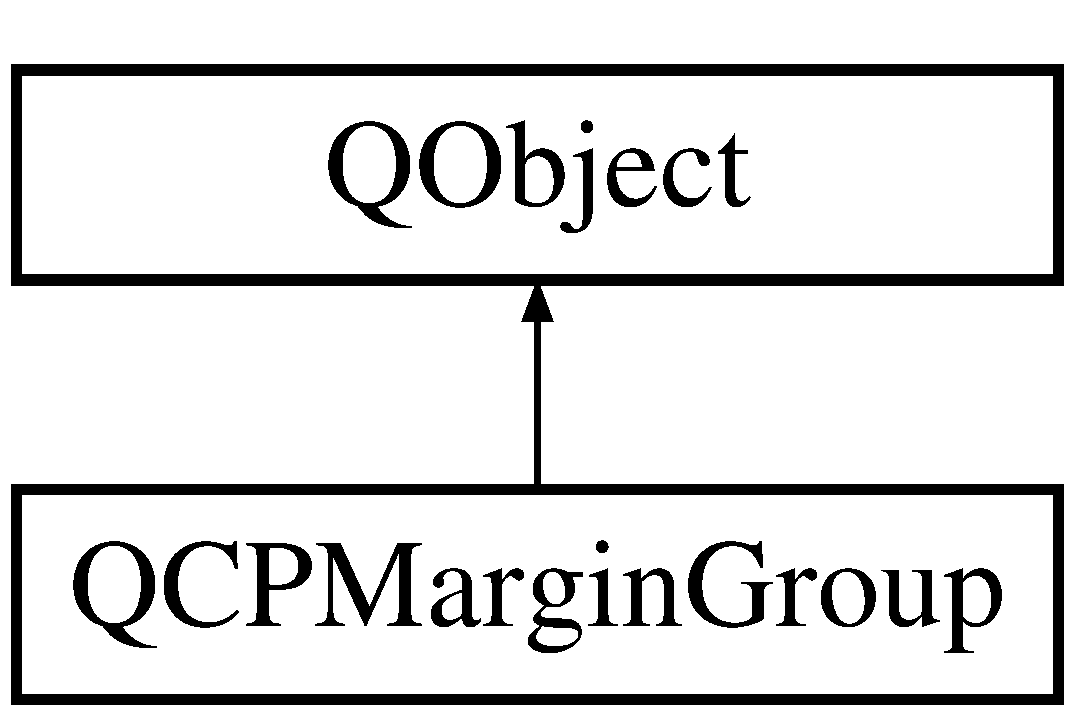
\includegraphics[height=2.000000cm]{class_q_c_p_margin_group}
\end{center}
\end{figure}
\subsection*{Public Member Functions}
\begin{DoxyCompactItemize}
\item 
\hyperlink{class_q_c_p_margin_group_ac481c20678ec5b305d6df330715f4b7b}{Q\+C\+P\+Margin\+Group} (\hyperlink{class_q_custom_plot}{Q\+Custom\+Plot} $\ast$parent\+Plot)
\item 
Q\+List$<$ \hyperlink{class_q_c_p_layout_element}{Q\+C\+P\+Layout\+Element} $\ast$ $>$ \hyperlink{class_q_c_p_margin_group_ac967a4dc5fe02ae44aeb43511d5e1bd4}{elements} (\hyperlink{namespace_q_c_p_a7e487e3e2ccb62ab7771065bab7cae54}{Q\+C\+P\+::\+Margin\+Side} side) const
\item 
bool \hyperlink{class_q_c_p_margin_group_ae0d32656d8a5fc5690c4e7693f9d0539}{is\+Empty} () const
\item 
void \hyperlink{class_q_c_p_margin_group_a144b67f216e4e86c3a3a309e850285fe}{clear} ()
\end{DoxyCompactItemize}
\subsection*{Protected Member Functions}
\begin{DoxyCompactItemize}
\item 
\hypertarget{class_q_c_p_margin_group_aea6a00373b3a0305de56c34d2423ea99}{}\label{class_q_c_p_margin_group_aea6a00373b3a0305de56c34d2423ea99} 
int {\bfseries common\+Margin} (\hyperlink{namespace_q_c_p_a7e487e3e2ccb62ab7771065bab7cae54}{Q\+C\+P\+::\+Margin\+Side} side) const
\item 
\hypertarget{class_q_c_p_margin_group_acb9c3a35acec655c2895b7eb95ee0524}{}\label{class_q_c_p_margin_group_acb9c3a35acec655c2895b7eb95ee0524} 
void {\bfseries add\+Child} (\hyperlink{namespace_q_c_p_a7e487e3e2ccb62ab7771065bab7cae54}{Q\+C\+P\+::\+Margin\+Side} side, \hyperlink{class_q_c_p_layout_element}{Q\+C\+P\+Layout\+Element} $\ast$element)
\item 
\hypertarget{class_q_c_p_margin_group_a20ab3286062957d99b58db683fe725b0}{}\label{class_q_c_p_margin_group_a20ab3286062957d99b58db683fe725b0} 
void {\bfseries remove\+Child} (\hyperlink{namespace_q_c_p_a7e487e3e2ccb62ab7771065bab7cae54}{Q\+C\+P\+::\+Margin\+Side} side, \hyperlink{class_q_c_p_layout_element}{Q\+C\+P\+Layout\+Element} $\ast$element)
\end{DoxyCompactItemize}
\subsection*{Protected Attributes}
\begin{DoxyCompactItemize}
\item 
\hypertarget{class_q_c_p_margin_group_a23cfa29e3cc0f33a59141b77d8c04edf}{}\label{class_q_c_p_margin_group_a23cfa29e3cc0f33a59141b77d8c04edf} 
\hyperlink{class_q_custom_plot}{Q\+Custom\+Plot} $\ast$ {\bfseries m\+Parent\+Plot}
\item 
\hypertarget{class_q_c_p_margin_group_a954bc89ff8958b9bb6a4a0d08ed5fc0f}{}\label{class_q_c_p_margin_group_a954bc89ff8958b9bb6a4a0d08ed5fc0f} 
Q\+Hash$<$ \hyperlink{namespace_q_c_p_a7e487e3e2ccb62ab7771065bab7cae54}{Q\+C\+P\+::\+Margin\+Side}, Q\+List$<$ \hyperlink{class_q_c_p_layout_element}{Q\+C\+P\+Layout\+Element} $\ast$ $>$ $>$ {\bfseries m\+Children}
\end{DoxyCompactItemize}
\subsection*{Friends}
\begin{DoxyCompactItemize}
\item 
\hypertarget{class_q_c_p_margin_group_a0790750c7e7f14fdbd960d172655b42b}{}\label{class_q_c_p_margin_group_a0790750c7e7f14fdbd960d172655b42b} 
class {\bfseries Q\+C\+P\+Layout\+Element}
\end{DoxyCompactItemize}


\subsection{Detailed Description}
A margin group allows synchronization of margin sides if working with multiple layout elements. 

\hyperlink{class_q_c_p_margin_group}{Q\+C\+P\+Margin\+Group} allows you to tie a margin side of two or more layout elements together, such that they will all have the same size, based on the largest required margin in the group.

~\newline
~\newline
 In certain situations it is desirable that margins at specific sides are synchronized across layout elements. For example, if one \hyperlink{class_q_c_p_axis_rect}{Q\+C\+P\+Axis\+Rect} is below another one in a grid layout, it will provide a cleaner look to the user if the left and right margins of the two axis rects are of the same size. The left axis of the top axis rect will then be at the same horizontal position as the left axis of the lower axis rect, making them appear aligned. The same applies for the right axes. This is what \hyperlink{class_q_c_p_margin_group}{Q\+C\+P\+Margin\+Group} makes possible.

To add/remove a specific side of a layout element to/from a margin group, use the \hyperlink{class_q_c_p_layout_element_a516e56f76b6bc100e8e71d329866847d}{Q\+C\+P\+Layout\+Element\+::set\+Margin\+Group} method. To completely break apart the margin group, either call \hyperlink{class_q_c_p_margin_group_a144b67f216e4e86c3a3a309e850285fe}{clear}, or just delete the margin group.\hypertarget{class_q_c_p_margin_group_QCPMarginGroup-example}{}\subsection{Example}\label{class_q_c_p_margin_group_QCPMarginGroup-example}
First create a margin group\+: 
\begin{DoxyCodeInclude}
\end{DoxyCodeInclude}
Then set this group on the layout element sides\+: 
\begin{DoxyCodeInclude}
\end{DoxyCodeInclude}
Here, we\textquotesingle{}ve used the first two axis rects of the plot and synchronized their left margins with each other and their right margins with each other. 

\subsection{Constructor \& Destructor Documentation}
\hypertarget{class_q_c_p_margin_group_ac481c20678ec5b305d6df330715f4b7b}{}\label{class_q_c_p_margin_group_ac481c20678ec5b305d6df330715f4b7b} 
\index{Q\+C\+P\+Margin\+Group@{Q\+C\+P\+Margin\+Group}!Q\+C\+P\+Margin\+Group@{Q\+C\+P\+Margin\+Group}}
\index{Q\+C\+P\+Margin\+Group@{Q\+C\+P\+Margin\+Group}!Q\+C\+P\+Margin\+Group@{Q\+C\+P\+Margin\+Group}}
\subsubsection{\texorpdfstring{Q\+C\+P\+Margin\+Group()}{QCPMarginGroup()}}
{\footnotesize\ttfamily Q\+C\+P\+Margin\+Group\+::\+Q\+C\+P\+Margin\+Group (\begin{DoxyParamCaption}\item[{\hyperlink{class_q_custom_plot}{Q\+Custom\+Plot} $\ast$}]{parent\+Plot }\end{DoxyParamCaption})}

Creates a new \hyperlink{class_q_c_p_margin_group}{Q\+C\+P\+Margin\+Group} instance in {\itshape parent\+Plot}. 

\subsection{Member Function Documentation}
\hypertarget{class_q_c_p_margin_group_a144b67f216e4e86c3a3a309e850285fe}{}\label{class_q_c_p_margin_group_a144b67f216e4e86c3a3a309e850285fe} 
\index{Q\+C\+P\+Margin\+Group@{Q\+C\+P\+Margin\+Group}!clear@{clear}}
\index{clear@{clear}!Q\+C\+P\+Margin\+Group@{Q\+C\+P\+Margin\+Group}}
\subsubsection{\texorpdfstring{clear()}{clear()}}
{\footnotesize\ttfamily void Q\+C\+P\+Margin\+Group\+::clear (\begin{DoxyParamCaption}{ }\end{DoxyParamCaption})}

Clears this margin group. The synchronization of the margin sides that use this margin group is lifted and they will use their individual margin sizes again. \hypertarget{class_q_c_p_margin_group_ac967a4dc5fe02ae44aeb43511d5e1bd4}{}\label{class_q_c_p_margin_group_ac967a4dc5fe02ae44aeb43511d5e1bd4} 
\index{Q\+C\+P\+Margin\+Group@{Q\+C\+P\+Margin\+Group}!elements@{elements}}
\index{elements@{elements}!Q\+C\+P\+Margin\+Group@{Q\+C\+P\+Margin\+Group}}
\subsubsection{\texorpdfstring{elements()}{elements()}}
{\footnotesize\ttfamily Q\+List$<$ \hyperlink{class_q_c_p_layout_element}{Q\+C\+P\+Layout\+Element} $\ast$ $>$ Q\+C\+P\+Margin\+Group\+::elements (\begin{DoxyParamCaption}\item[{\hyperlink{namespace_q_c_p_a7e487e3e2ccb62ab7771065bab7cae54}{Q\+C\+P\+::\+Margin\+Side}}]{side }\end{DoxyParamCaption}) const\hspace{0.3cm}{\ttfamily [inline]}}

Returns a list of all layout elements that have their margin {\itshape side} associated with this margin group. \hypertarget{class_q_c_p_margin_group_ae0d32656d8a5fc5690c4e7693f9d0539}{}\label{class_q_c_p_margin_group_ae0d32656d8a5fc5690c4e7693f9d0539} 
\index{Q\+C\+P\+Margin\+Group@{Q\+C\+P\+Margin\+Group}!is\+Empty@{is\+Empty}}
\index{is\+Empty@{is\+Empty}!Q\+C\+P\+Margin\+Group@{Q\+C\+P\+Margin\+Group}}
\subsubsection{\texorpdfstring{is\+Empty()}{isEmpty()}}
{\footnotesize\ttfamily bool Q\+C\+P\+Margin\+Group\+::is\+Empty (\begin{DoxyParamCaption}{ }\end{DoxyParamCaption}) const}

Returns whether this margin group is empty. If this function returns true, no layout elements use this margin group to synchronize margin sides. 

The documentation for this class was generated from the following files\+:\begin{DoxyCompactItemize}
\item 
C\+:/\+Users/\+Jesse Jutson/\+Documents/\+Git\+Hub/\+F\+E\+S\+S\+G\+U\+I/\+F\+E\+S\+S-\/\+G\+U\+I/\hyperlink{qcustomplot_8h}{qcustomplot.\+h}\item 
C\+:/\+Users/\+Jesse Jutson/\+Documents/\+Git\+Hub/\+F\+E\+S\+S\+G\+U\+I/\+F\+E\+S\+S-\/\+G\+U\+I/\hyperlink{qcustomplot_8cpp}{qcustomplot.\+cpp}\end{DoxyCompactItemize}

\hypertarget{class_q_c_p_painter}{}\section{Q\+C\+P\+Painter Class Reference}
\label{class_q_c_p_painter}\index{Q\+C\+P\+Painter@{Q\+C\+P\+Painter}}


Q\+Painter subclass used internally.  


Inheritance diagram for Q\+C\+P\+Painter\+:\begin{figure}[H]
\begin{center}
\leavevmode
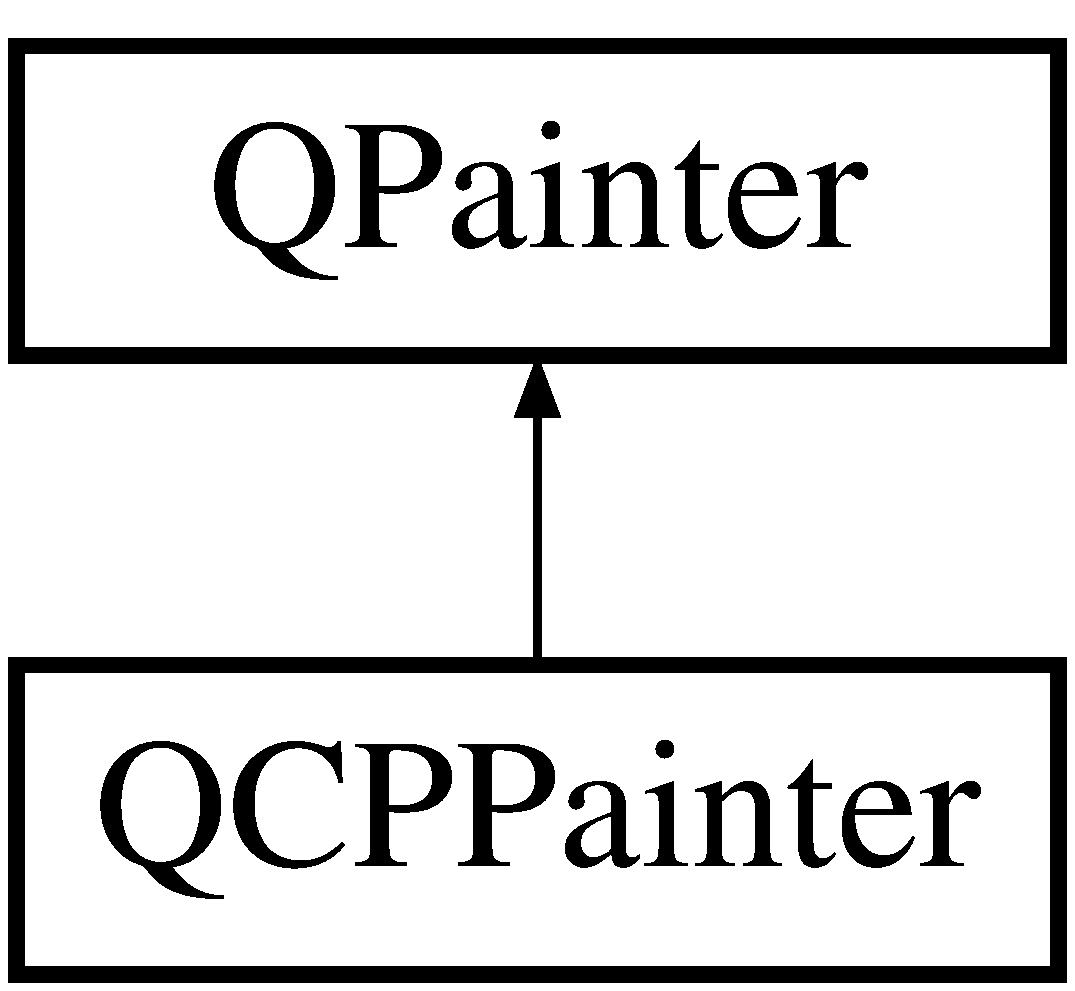
\includegraphics[height=2.000000cm]{class_q_c_p_painter}
\end{center}
\end{figure}
\subsection*{Public Types}
\begin{DoxyCompactItemize}
\item 
enum \hyperlink{class_q_c_p_painter_a156cf16444ff5e0d81a73c615fdb156d}{Painter\+Mode} \{ \hyperlink{class_q_c_p_painter_a156cf16444ff5e0d81a73c615fdb156da3bac5e87e3d58553b297befb4eee2a45}{pm\+Default} = 0x00, 
\hyperlink{class_q_c_p_painter_a156cf16444ff5e0d81a73c615fdb156daeda679cd55dcd468341d07d48a30b6ab}{pm\+Vectorized} = 0x01, 
\hyperlink{class_q_c_p_painter_a156cf16444ff5e0d81a73c615fdb156dae78f9a4eb277a5f9207f50850a51a0b0}{pm\+No\+Caching} = 0x02, 
\hyperlink{class_q_c_p_painter_a156cf16444ff5e0d81a73c615fdb156dac1e481bfaf408f2bd2eaad3ec341f36b}{pm\+Non\+Cosmetic} = 0x04
 \}
\end{DoxyCompactItemize}
\subsection*{Public Member Functions}
\begin{DoxyCompactItemize}
\item 
\hyperlink{class_q_c_p_painter_a3c52cb0f43f34573d29bea487da28fe8}{Q\+C\+P\+Painter} ()
\item 
\hyperlink{class_q_c_p_painter_ae58dbb1795ddc4351ab324dc9898aa22}{Q\+C\+P\+Painter} (Q\+Paint\+Device $\ast$device)
\item 
\hypertarget{class_q_c_p_painter_a5aff96296e995f6f35b2596a482aae37}{}\label{class_q_c_p_painter_a5aff96296e995f6f35b2596a482aae37} 
bool {\bfseries antialiasing} () const
\item 
\hypertarget{class_q_c_p_painter_aef102658219b24165f7ee2aad1b9e48f}{}\label{class_q_c_p_painter_aef102658219b24165f7ee2aad1b9e48f} 
Painter\+Modes {\bfseries modes} () const
\item 
void \hyperlink{class_q_c_p_painter_aaba1deb9188244d9ea65b035112b4d05}{set\+Antialiasing} (bool enabled)
\item 
void \hyperlink{class_q_c_p_painter_af6b1f7d2bbc548b10aa55d8b6ad49577}{set\+Mode} (\hyperlink{class_q_c_p_painter_a156cf16444ff5e0d81a73c615fdb156d}{Painter\+Mode} mode, bool enabled=true)
\item 
void \hyperlink{class_q_c_p_painter_a5fac93adc29c7c4dea9f3e171e9e635e}{set\+Modes} (Painter\+Modes modes)
\item 
bool \hyperlink{class_q_c_p_painter_a0a41146ccd619dceab6e25ec7b46b044}{begin} (Q\+Paint\+Device $\ast$device)
\item 
void \hyperlink{class_q_c_p_painter_af9c7a4cd1791403901f8c5b82a150195}{set\+Pen} (const Q\+Pen \&pen)
\item 
void \hyperlink{class_q_c_p_painter_a5c4d88f21564e156e88ef807f7cf0003}{set\+Pen} (const Q\+Color \&color)
\item 
void \hyperlink{class_q_c_p_painter_a25e76095aae41da0d08035060e5f81ca}{set\+Pen} (Qt\+::\+Pen\+Style pen\+Style)
\item 
void \hyperlink{class_q_c_p_painter_a0b4b1b9bd495e182c731774dc800e6e0}{draw\+Line} (const Q\+LineF \&line)
\item 
\hypertarget{class_q_c_p_painter_ad1638db27929491b3f1beb74d6cbad5e}{}\label{class_q_c_p_painter_ad1638db27929491b3f1beb74d6cbad5e} 
void {\bfseries draw\+Line} (const Q\+PointF \&p1, const Q\+PointF \&p2)
\item 
void \hyperlink{class_q_c_p_painter_a8fd6821ee6fecbfa04444c9062912abd}{save} ()
\item 
void \hyperlink{class_q_c_p_painter_a64908e6298d5bbd83457dc987cc3a022}{restore} ()
\item 
void \hyperlink{class_q_c_p_painter_a7e63fbcf47e35c6f2ecd11b8fef7c7d8}{make\+Non\+Cosmetic} ()
\end{DoxyCompactItemize}
\subsection*{Protected Attributes}
\begin{DoxyCompactItemize}
\item 
\hypertarget{class_q_c_p_painter_af5d1d6e5df0adbc7de5633250fb3396c}{}\label{class_q_c_p_painter_af5d1d6e5df0adbc7de5633250fb3396c} 
Painter\+Modes {\bfseries m\+Modes}
\item 
\hypertarget{class_q_c_p_painter_a7055085da176aee0f6b23298f1003d08}{}\label{class_q_c_p_painter_a7055085da176aee0f6b23298f1003d08} 
bool {\bfseries m\+Is\+Antialiasing}
\item 
\hypertarget{class_q_c_p_painter_a0189e641bbf7dc31ac15aef7b36501fa}{}\label{class_q_c_p_painter_a0189e641bbf7dc31ac15aef7b36501fa} 
Q\+Stack$<$ bool $>$ {\bfseries m\+Antialiasing\+Stack}
\end{DoxyCompactItemize}


\subsection{Detailed Description}
Q\+Painter subclass used internally. 

This Q\+Painter subclass is used to provide some extended functionality e.\+g. for tweaking position consistency between antialiased and non-\/antialiased painting. Further it provides workarounds for Q\+Painter quirks.

\begin{DoxyWarning}{Warning}
This class intentionally hides non-\/virtual functions of Q\+Painter, e.\+g. set\+Pen, save and restore. So while it is possible to pass a \hyperlink{class_q_c_p_painter}{Q\+C\+P\+Painter} instance to a function that expects a Q\+Painter pointer, some of the workarounds and tweaks will be unavailable to the function (because it will call the base class implementations of the functions actually hidden by \hyperlink{class_q_c_p_painter}{Q\+C\+P\+Painter}). 
\end{DoxyWarning}


\subsection{Member Enumeration Documentation}
\hypertarget{class_q_c_p_painter_a156cf16444ff5e0d81a73c615fdb156d}{}\label{class_q_c_p_painter_a156cf16444ff5e0d81a73c615fdb156d} 
\index{Q\+C\+P\+Painter@{Q\+C\+P\+Painter}!Painter\+Mode@{Painter\+Mode}}
\index{Painter\+Mode@{Painter\+Mode}!Q\+C\+P\+Painter@{Q\+C\+P\+Painter}}
\subsubsection{\texorpdfstring{Painter\+Mode}{PainterMode}}
{\footnotesize\ttfamily enum \hyperlink{class_q_c_p_painter_a156cf16444ff5e0d81a73c615fdb156d}{Q\+C\+P\+Painter\+::\+Painter\+Mode}}

Defines special modes the painter can operate in. They disable or enable certain subsets of features/fixes/workarounds, depending on whether they are wanted on the respective output device. \begin{DoxyEnumFields}{Enumerator}
\raisebox{\heightof{T}}[0pt][0pt]{\index{pm\+Default@{pm\+Default}!Q\+C\+P\+Painter@{Q\+C\+P\+Painter}}\index{Q\+C\+P\+Painter@{Q\+C\+P\+Painter}!pm\+Default@{pm\+Default}}}\hypertarget{class_q_c_p_painter_a156cf16444ff5e0d81a73c615fdb156da3bac5e87e3d58553b297befb4eee2a45}{}\label{class_q_c_p_painter_a156cf16444ff5e0d81a73c615fdb156da3bac5e87e3d58553b297befb4eee2a45} 
pm\+Default&{\ttfamily 0x00} Default mode for painting on screen devices \\
\hline

\raisebox{\heightof{T}}[0pt][0pt]{\index{pm\+Vectorized@{pm\+Vectorized}!Q\+C\+P\+Painter@{Q\+C\+P\+Painter}}\index{Q\+C\+P\+Painter@{Q\+C\+P\+Painter}!pm\+Vectorized@{pm\+Vectorized}}}\hypertarget{class_q_c_p_painter_a156cf16444ff5e0d81a73c615fdb156daeda679cd55dcd468341d07d48a30b6ab}{}\label{class_q_c_p_painter_a156cf16444ff5e0d81a73c615fdb156daeda679cd55dcd468341d07d48a30b6ab} 
pm\+Vectorized&{\ttfamily 0x01} Mode for vectorized painting (e.\+g. P\+DF export). For example, this prevents some antialiasing fixes. \\
\hline

\raisebox{\heightof{T}}[0pt][0pt]{\index{pm\+No\+Caching@{pm\+No\+Caching}!Q\+C\+P\+Painter@{Q\+C\+P\+Painter}}\index{Q\+C\+P\+Painter@{Q\+C\+P\+Painter}!pm\+No\+Caching@{pm\+No\+Caching}}}\hypertarget{class_q_c_p_painter_a156cf16444ff5e0d81a73c615fdb156dae78f9a4eb277a5f9207f50850a51a0b0}{}\label{class_q_c_p_painter_a156cf16444ff5e0d81a73c615fdb156dae78f9a4eb277a5f9207f50850a51a0b0} 
pm\+No\+Caching&{\ttfamily 0x02} Mode for all sorts of exports (e.\+g. P\+NG, P\+DF,...). For example, this prevents using cached pixmap labels \\
\hline

\raisebox{\heightof{T}}[0pt][0pt]{\index{pm\+Non\+Cosmetic@{pm\+Non\+Cosmetic}!Q\+C\+P\+Painter@{Q\+C\+P\+Painter}}\index{Q\+C\+P\+Painter@{Q\+C\+P\+Painter}!pm\+Non\+Cosmetic@{pm\+Non\+Cosmetic}}}\hypertarget{class_q_c_p_painter_a156cf16444ff5e0d81a73c615fdb156dac1e481bfaf408f2bd2eaad3ec341f36b}{}\label{class_q_c_p_painter_a156cf16444ff5e0d81a73c615fdb156dac1e481bfaf408f2bd2eaad3ec341f36b} 
pm\+Non\+Cosmetic&{\ttfamily 0x04} Turns pen widths 0 to 1, i.\+e. disables cosmetic pens. (A cosmetic pen is always drawn with width 1 pixel in the vector image/pdf viewer, independent of zoom.) \\
\hline

\end{DoxyEnumFields}


\subsection{Constructor \& Destructor Documentation}
\hypertarget{class_q_c_p_painter_a3c52cb0f43f34573d29bea487da28fe8}{}\label{class_q_c_p_painter_a3c52cb0f43f34573d29bea487da28fe8} 
\index{Q\+C\+P\+Painter@{Q\+C\+P\+Painter}!Q\+C\+P\+Painter@{Q\+C\+P\+Painter}}
\index{Q\+C\+P\+Painter@{Q\+C\+P\+Painter}!Q\+C\+P\+Painter@{Q\+C\+P\+Painter}}
\subsubsection{\texorpdfstring{Q\+C\+P\+Painter()}{QCPPainter()}\hspace{0.1cm}{\footnotesize\ttfamily [1/2]}}
{\footnotesize\ttfamily Q\+C\+P\+Painter\+::\+Q\+C\+P\+Painter (\begin{DoxyParamCaption}{ }\end{DoxyParamCaption})}

Creates a new \hyperlink{class_q_c_p_painter}{Q\+C\+P\+Painter} instance and sets default values \hypertarget{class_q_c_p_painter_ae58dbb1795ddc4351ab324dc9898aa22}{}\label{class_q_c_p_painter_ae58dbb1795ddc4351ab324dc9898aa22} 
\index{Q\+C\+P\+Painter@{Q\+C\+P\+Painter}!Q\+C\+P\+Painter@{Q\+C\+P\+Painter}}
\index{Q\+C\+P\+Painter@{Q\+C\+P\+Painter}!Q\+C\+P\+Painter@{Q\+C\+P\+Painter}}
\subsubsection{\texorpdfstring{Q\+C\+P\+Painter()}{QCPPainter()}\hspace{0.1cm}{\footnotesize\ttfamily [2/2]}}
{\footnotesize\ttfamily Q\+C\+P\+Painter\+::\+Q\+C\+P\+Painter (\begin{DoxyParamCaption}\item[{Q\+Paint\+Device $\ast$}]{device }\end{DoxyParamCaption})}

Creates a new \hyperlink{class_q_c_p_painter}{Q\+C\+P\+Painter} instance on the specified paint {\itshape device} and sets default values. Just like the analogous Q\+Painter constructor, begins painting on {\itshape device} immediately.

Like \hyperlink{class_q_c_p_painter_a0a41146ccd619dceab6e25ec7b46b044}{begin}, this method sets Q\+Painter\+::\+Non\+Cosmetic\+Default\+Pen in Qt versions before Qt5. 

\subsection{Member Function Documentation}
\hypertarget{class_q_c_p_painter_a0a41146ccd619dceab6e25ec7b46b044}{}\label{class_q_c_p_painter_a0a41146ccd619dceab6e25ec7b46b044} 
\index{Q\+C\+P\+Painter@{Q\+C\+P\+Painter}!begin@{begin}}
\index{begin@{begin}!Q\+C\+P\+Painter@{Q\+C\+P\+Painter}}
\subsubsection{\texorpdfstring{begin()}{begin()}}
{\footnotesize\ttfamily bool Q\+C\+P\+Painter\+::begin (\begin{DoxyParamCaption}\item[{Q\+Paint\+Device $\ast$}]{device }\end{DoxyParamCaption})}

Sets the Q\+Painter\+::\+Non\+Cosmetic\+Default\+Pen in Qt versions before Qt5 after beginning painting on {\itshape device}. This is necessary to get cosmetic pen consistency across Qt versions, because since Qt5, all pens are non-\/cosmetic by default, and in Qt4 this render hint must be set to get that behaviour.

The Constructor \hyperlink{class_q_c_p_painter_ae58dbb1795ddc4351ab324dc9898aa22}{Q\+C\+P\+Painter(\+Q\+Paint\+Device $\ast$device)} which directly starts painting also sets the render hint as appropriate.

\begin{DoxyNote}{Note}
this function hides the non-\/virtual base class implementation. 
\end{DoxyNote}
\hypertarget{class_q_c_p_painter_a0b4b1b9bd495e182c731774dc800e6e0}{}\label{class_q_c_p_painter_a0b4b1b9bd495e182c731774dc800e6e0} 
\index{Q\+C\+P\+Painter@{Q\+C\+P\+Painter}!draw\+Line@{draw\+Line}}
\index{draw\+Line@{draw\+Line}!Q\+C\+P\+Painter@{Q\+C\+P\+Painter}}
\subsubsection{\texorpdfstring{draw\+Line()}{drawLine()}}
{\footnotesize\ttfamily void Q\+C\+P\+Painter\+::draw\+Line (\begin{DoxyParamCaption}\item[{const Q\+LineF \&}]{line }\end{DoxyParamCaption})}

This is an overloaded member function, provided for convenience. It differs from the above function only in what argument(s) it accepts.

Works around a Qt bug introduced with Qt 4.\+8 which makes drawing Q\+LineF unpredictable when antialiasing is disabled. Thus when antialiasing is disabled, it rounds the {\itshape line} to integer coordinates and then passes it to the original draw\+Line.

\begin{DoxyNote}{Note}
this function hides the non-\/virtual base class implementation. 
\end{DoxyNote}
\hypertarget{class_q_c_p_painter_a7e63fbcf47e35c6f2ecd11b8fef7c7d8}{}\label{class_q_c_p_painter_a7e63fbcf47e35c6f2ecd11b8fef7c7d8} 
\index{Q\+C\+P\+Painter@{Q\+C\+P\+Painter}!make\+Non\+Cosmetic@{make\+Non\+Cosmetic}}
\index{make\+Non\+Cosmetic@{make\+Non\+Cosmetic}!Q\+C\+P\+Painter@{Q\+C\+P\+Painter}}
\subsubsection{\texorpdfstring{make\+Non\+Cosmetic()}{makeNonCosmetic()}}
{\footnotesize\ttfamily void Q\+C\+P\+Painter\+::make\+Non\+Cosmetic (\begin{DoxyParamCaption}{ }\end{DoxyParamCaption})}

Changes the pen width to 1 if it currently is 0. This function is called in the \hyperlink{class_q_c_p_painter_af9c7a4cd1791403901f8c5b82a150195}{set\+Pen} overrides when the \hyperlink{class_q_c_p_painter_a156cf16444ff5e0d81a73c615fdb156dac1e481bfaf408f2bd2eaad3ec341f36b}{pm\+Non\+Cosmetic} mode is set. \hypertarget{class_q_c_p_painter_a64908e6298d5bbd83457dc987cc3a022}{}\label{class_q_c_p_painter_a64908e6298d5bbd83457dc987cc3a022} 
\index{Q\+C\+P\+Painter@{Q\+C\+P\+Painter}!restore@{restore}}
\index{restore@{restore}!Q\+C\+P\+Painter@{Q\+C\+P\+Painter}}
\subsubsection{\texorpdfstring{restore()}{restore()}}
{\footnotesize\ttfamily void Q\+C\+P\+Painter\+::restore (\begin{DoxyParamCaption}{ }\end{DoxyParamCaption})}

Restores the painter (see Q\+Painter\+::restore). Since \hyperlink{class_q_c_p_painter}{Q\+C\+P\+Painter} adds some new internal state to Q\+Painter, the save/restore functions are reimplemented to also save/restore those members.

\begin{DoxyNote}{Note}
this function hides the non-\/virtual base class implementation.
\end{DoxyNote}
\begin{DoxySeeAlso}{See also}
\hyperlink{class_q_c_p_painter_a8fd6821ee6fecbfa04444c9062912abd}{save} 
\end{DoxySeeAlso}
\hypertarget{class_q_c_p_painter_a8fd6821ee6fecbfa04444c9062912abd}{}\label{class_q_c_p_painter_a8fd6821ee6fecbfa04444c9062912abd} 
\index{Q\+C\+P\+Painter@{Q\+C\+P\+Painter}!save@{save}}
\index{save@{save}!Q\+C\+P\+Painter@{Q\+C\+P\+Painter}}
\subsubsection{\texorpdfstring{save()}{save()}}
{\footnotesize\ttfamily void Q\+C\+P\+Painter\+::save (\begin{DoxyParamCaption}{ }\end{DoxyParamCaption})}

Saves the painter (see Q\+Painter\+::save). Since \hyperlink{class_q_c_p_painter}{Q\+C\+P\+Painter} adds some new internal state to Q\+Painter, the save/restore functions are reimplemented to also save/restore those members.

\begin{DoxyNote}{Note}
this function hides the non-\/virtual base class implementation.
\end{DoxyNote}
\begin{DoxySeeAlso}{See also}
\hyperlink{class_q_c_p_painter_a64908e6298d5bbd83457dc987cc3a022}{restore} 
\end{DoxySeeAlso}
\hypertarget{class_q_c_p_painter_aaba1deb9188244d9ea65b035112b4d05}{}\label{class_q_c_p_painter_aaba1deb9188244d9ea65b035112b4d05} 
\index{Q\+C\+P\+Painter@{Q\+C\+P\+Painter}!set\+Antialiasing@{set\+Antialiasing}}
\index{set\+Antialiasing@{set\+Antialiasing}!Q\+C\+P\+Painter@{Q\+C\+P\+Painter}}
\subsubsection{\texorpdfstring{set\+Antialiasing()}{setAntialiasing()}}
{\footnotesize\ttfamily void Q\+C\+P\+Painter\+::set\+Antialiasing (\begin{DoxyParamCaption}\item[{bool}]{enabled }\end{DoxyParamCaption})}

Sets whether painting uses antialiasing or not. Use this method instead of using set\+Render\+Hint with Q\+Painter\+::\+Antialiasing directly, as it allows \hyperlink{class_q_c_p_painter}{Q\+C\+P\+Painter} to regain pixel exactness between antialiased and non-\/antialiased painting (Since Qt $<$ 5.\+0 uses slightly different coordinate systems for A\+A/\+Non-\/\+AA painting). \hypertarget{class_q_c_p_painter_af6b1f7d2bbc548b10aa55d8b6ad49577}{}\label{class_q_c_p_painter_af6b1f7d2bbc548b10aa55d8b6ad49577} 
\index{Q\+C\+P\+Painter@{Q\+C\+P\+Painter}!set\+Mode@{set\+Mode}}
\index{set\+Mode@{set\+Mode}!Q\+C\+P\+Painter@{Q\+C\+P\+Painter}}
\subsubsection{\texorpdfstring{set\+Mode()}{setMode()}}
{\footnotesize\ttfamily void Q\+C\+P\+Painter\+::set\+Mode (\begin{DoxyParamCaption}\item[{\hyperlink{class_q_c_p_painter_a156cf16444ff5e0d81a73c615fdb156d}{Q\+C\+P\+Painter\+::\+Painter\+Mode}}]{mode,  }\item[{bool}]{enabled = {\ttfamily true} }\end{DoxyParamCaption})}

This is an overloaded member function, provided for convenience. It differs from the above function only in what argument(s) it accepts.

Sets the mode of the painter. This controls whether the painter shall adjust its fixes/workarounds optimized for certain output devices. \hypertarget{class_q_c_p_painter_a5fac93adc29c7c4dea9f3e171e9e635e}{}\label{class_q_c_p_painter_a5fac93adc29c7c4dea9f3e171e9e635e} 
\index{Q\+C\+P\+Painter@{Q\+C\+P\+Painter}!set\+Modes@{set\+Modes}}
\index{set\+Modes@{set\+Modes}!Q\+C\+P\+Painter@{Q\+C\+P\+Painter}}
\subsubsection{\texorpdfstring{set\+Modes()}{setModes()}}
{\footnotesize\ttfamily void Q\+C\+P\+Painter\+::set\+Modes (\begin{DoxyParamCaption}\item[{Painter\+Modes}]{modes }\end{DoxyParamCaption})}

Sets the mode of the painter. This controls whether the painter shall adjust its fixes/workarounds optimized for certain output devices. \hypertarget{class_q_c_p_painter_af9c7a4cd1791403901f8c5b82a150195}{}\label{class_q_c_p_painter_af9c7a4cd1791403901f8c5b82a150195} 
\index{Q\+C\+P\+Painter@{Q\+C\+P\+Painter}!set\+Pen@{set\+Pen}}
\index{set\+Pen@{set\+Pen}!Q\+C\+P\+Painter@{Q\+C\+P\+Painter}}
\subsubsection{\texorpdfstring{set\+Pen()}{setPen()}\hspace{0.1cm}{\footnotesize\ttfamily [1/3]}}
{\footnotesize\ttfamily void Q\+C\+P\+Painter\+::set\+Pen (\begin{DoxyParamCaption}\item[{const Q\+Pen \&}]{pen }\end{DoxyParamCaption})}

Sets the pen of the painter and applies certain fixes to it, depending on the mode of this \hyperlink{class_q_c_p_painter}{Q\+C\+P\+Painter}.

\begin{DoxyNote}{Note}
this function hides the non-\/virtual base class implementation. 
\end{DoxyNote}
\hypertarget{class_q_c_p_painter_a5c4d88f21564e156e88ef807f7cf0003}{}\label{class_q_c_p_painter_a5c4d88f21564e156e88ef807f7cf0003} 
\index{Q\+C\+P\+Painter@{Q\+C\+P\+Painter}!set\+Pen@{set\+Pen}}
\index{set\+Pen@{set\+Pen}!Q\+C\+P\+Painter@{Q\+C\+P\+Painter}}
\subsubsection{\texorpdfstring{set\+Pen()}{setPen()}\hspace{0.1cm}{\footnotesize\ttfamily [2/3]}}
{\footnotesize\ttfamily void Q\+C\+P\+Painter\+::set\+Pen (\begin{DoxyParamCaption}\item[{const Q\+Color \&}]{color }\end{DoxyParamCaption})}

This is an overloaded member function, provided for convenience. It differs from the above function only in what argument(s) it accepts.

Sets the pen (by color) of the painter and applies certain fixes to it, depending on the mode of this \hyperlink{class_q_c_p_painter}{Q\+C\+P\+Painter}.

\begin{DoxyNote}{Note}
this function hides the non-\/virtual base class implementation. 
\end{DoxyNote}
\hypertarget{class_q_c_p_painter_a25e76095aae41da0d08035060e5f81ca}{}\label{class_q_c_p_painter_a25e76095aae41da0d08035060e5f81ca} 
\index{Q\+C\+P\+Painter@{Q\+C\+P\+Painter}!set\+Pen@{set\+Pen}}
\index{set\+Pen@{set\+Pen}!Q\+C\+P\+Painter@{Q\+C\+P\+Painter}}
\subsubsection{\texorpdfstring{set\+Pen()}{setPen()}\hspace{0.1cm}{\footnotesize\ttfamily [3/3]}}
{\footnotesize\ttfamily void Q\+C\+P\+Painter\+::set\+Pen (\begin{DoxyParamCaption}\item[{Qt\+::\+Pen\+Style}]{pen\+Style }\end{DoxyParamCaption})}

This is an overloaded member function, provided for convenience. It differs from the above function only in what argument(s) it accepts.

Sets the pen (by style) of the painter and applies certain fixes to it, depending on the mode of this \hyperlink{class_q_c_p_painter}{Q\+C\+P\+Painter}.

\begin{DoxyNote}{Note}
this function hides the non-\/virtual base class implementation. 
\end{DoxyNote}


The documentation for this class was generated from the following files\+:\begin{DoxyCompactItemize}
\item 
C\+:/\+Users/\+Jesse Jutson/\+Documents/\+Git\+Hub/\+F\+E\+S\+S\+G\+U\+I/\+F\+E\+S\+S-\/\+G\+U\+I/\hyperlink{qcustomplot_8h}{qcustomplot.\+h}\item 
C\+:/\+Users/\+Jesse Jutson/\+Documents/\+Git\+Hub/\+F\+E\+S\+S\+G\+U\+I/\+F\+E\+S\+S-\/\+G\+U\+I/\hyperlink{qcustomplot_8cpp}{qcustomplot.\+cpp}\end{DoxyCompactItemize}

\hypertarget{class_q_c_p_plottable_legend_item}{}\section{Q\+C\+P\+Plottable\+Legend\+Item Class Reference}
\label{class_q_c_p_plottable_legend_item}\index{Q\+C\+P\+Plottable\+Legend\+Item@{Q\+C\+P\+Plottable\+Legend\+Item}}


A legend item representing a plottable with an icon and the plottable name.  


Inheritance diagram for Q\+C\+P\+Plottable\+Legend\+Item\+:\begin{figure}[H]
\begin{center}
\leavevmode
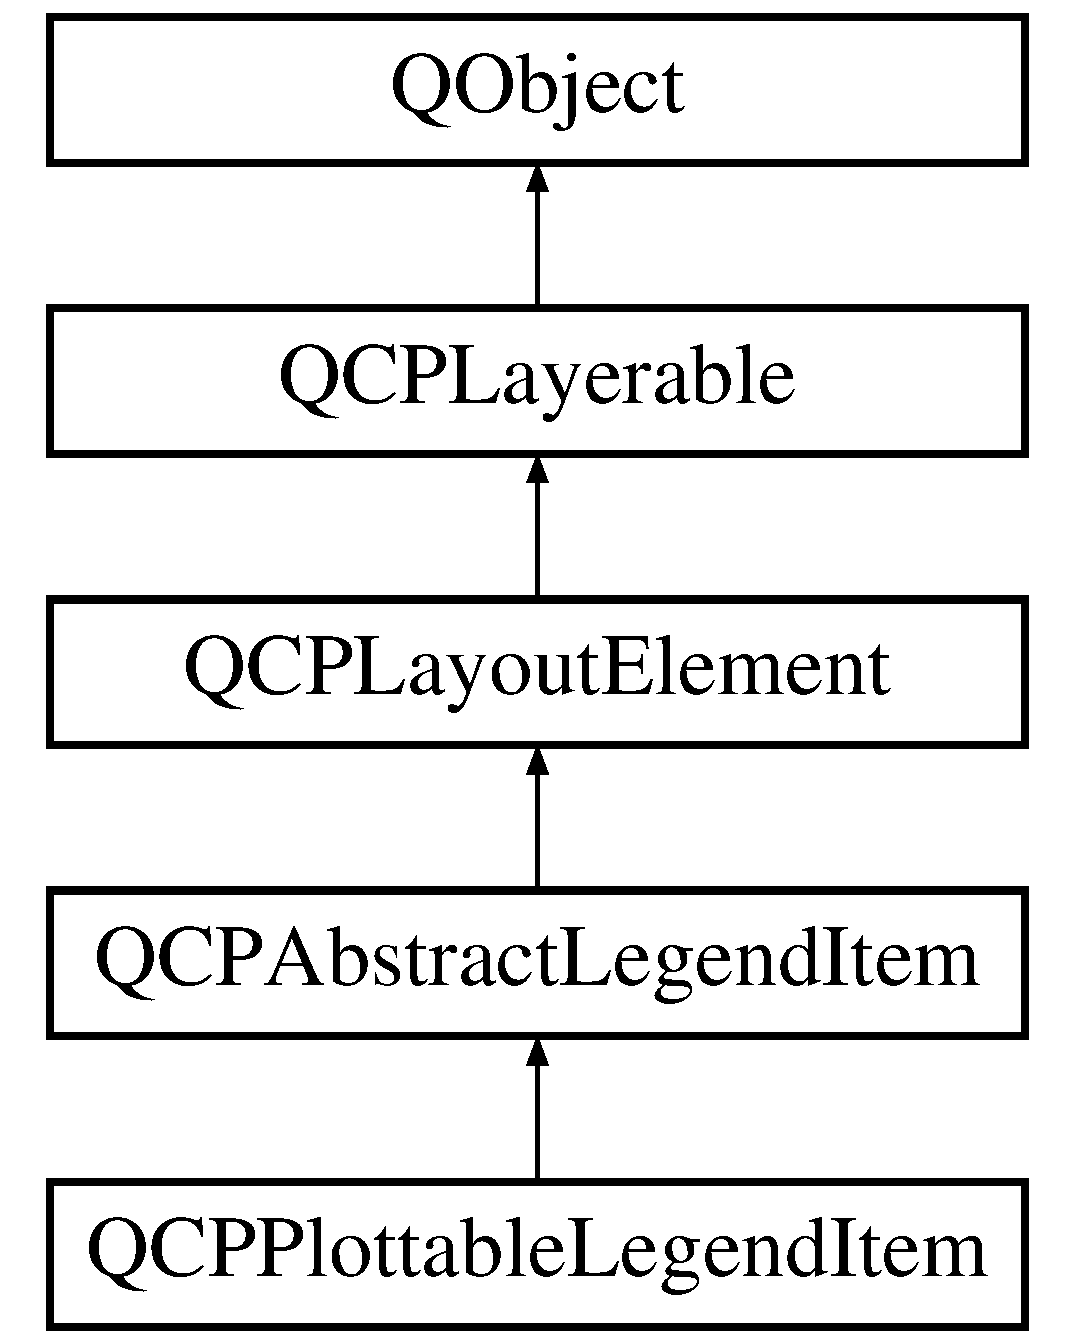
\includegraphics[height=5.000000cm]{class_q_c_p_plottable_legend_item}
\end{center}
\end{figure}
\subsection*{Public Member Functions}
\begin{DoxyCompactItemize}
\item 
\hyperlink{class_q_c_p_plottable_legend_item_ac1072591fe409d3dabad51b23ee4d6c5}{Q\+C\+P\+Plottable\+Legend\+Item} (\hyperlink{class_q_c_p_legend}{Q\+C\+P\+Legend} $\ast$parent, \hyperlink{class_q_c_p_abstract_plottable}{Q\+C\+P\+Abstract\+Plottable} $\ast$plottable)
\item 
\hypertarget{class_q_c_p_plottable_legend_item_af29e9a2c60b4cba0cac2447b8af7b488}{}\label{class_q_c_p_plottable_legend_item_af29e9a2c60b4cba0cac2447b8af7b488} 
\hyperlink{class_q_c_p_abstract_plottable}{Q\+C\+P\+Abstract\+Plottable} $\ast$ {\bfseries plottable} ()
\end{DoxyCompactItemize}
\subsection*{Protected Member Functions}
\begin{DoxyCompactItemize}
\item 
\hypertarget{class_q_c_p_plottable_legend_item_a68a781c3de4f9959fdf82075052d43aa}{}\label{class_q_c_p_plottable_legend_item_a68a781c3de4f9959fdf82075052d43aa} 
virtual void {\bfseries draw} (\hyperlink{class_q_c_p_painter}{Q\+C\+P\+Painter} $\ast$painter)
\item 
virtual Q\+Size \hyperlink{class_q_c_p_plottable_legend_item_a3adf8154c7e61538656d80464e5695dd}{minimum\+Size\+Hint} () const
\item 
\hypertarget{class_q_c_p_plottable_legend_item_afa81a8bd4434ec249efbbfc2a030a752}{}\label{class_q_c_p_plottable_legend_item_afa81a8bd4434ec249efbbfc2a030a752} 
Q\+Pen {\bfseries get\+Icon\+Border\+Pen} () const
\item 
\hypertarget{class_q_c_p_plottable_legend_item_a55daaffee35326765deebf8271efe210}{}\label{class_q_c_p_plottable_legend_item_a55daaffee35326765deebf8271efe210} 
Q\+Color {\bfseries get\+Text\+Color} () const
\item 
\hypertarget{class_q_c_p_plottable_legend_item_a77d980f594046226f9ac075fa07244b3}{}\label{class_q_c_p_plottable_legend_item_a77d980f594046226f9ac075fa07244b3} 
Q\+Font {\bfseries get\+Font} () const
\end{DoxyCompactItemize}
\subsection*{Protected Attributes}
\begin{DoxyCompactItemize}
\item 
\hypertarget{class_q_c_p_plottable_legend_item_ada647fb4b22971a1a424e15b4f6af0d9}{}\label{class_q_c_p_plottable_legend_item_ada647fb4b22971a1a424e15b4f6af0d9} 
\hyperlink{class_q_c_p_abstract_plottable}{Q\+C\+P\+Abstract\+Plottable} $\ast$ {\bfseries m\+Plottable}
\end{DoxyCompactItemize}
\subsection*{Additional Inherited Members}


\subsection{Detailed Description}
A legend item representing a plottable with an icon and the plottable name. 

This is the standard legend item for plottables. It displays an icon of the plottable next to the plottable name. The icon is drawn by the respective plottable itself (Q\+C\+P\+Abstract\+Plottable\+::draw\+Legend\+Icon), and tries to give an intuitive symbol for the plottable. For example, the \hyperlink{class_q_c_p_graph}{Q\+C\+P\+Graph} draws a centered horizontal line and/or a single scatter point in the middle.

Legend items of this type are always associated with one plottable (retrievable via the plottable() function and settable with the constructor). You may change the font of the plottable name with \hyperlink{class_q_c_p_abstract_legend_item_a409c53455d8112f71d70c0c43eb10265}{set\+Font}. Icon padding and border pen is taken from the parent \hyperlink{class_q_c_p_legend}{Q\+C\+P\+Legend}, see \hyperlink{class_q_c_p_legend_a2f2c93d18a651f4ff294bb3f026f49b8}{Q\+C\+P\+Legend\+::set\+Icon\+Border\+Pen} and \hyperlink{class_q_c_p_legend_a62973bd69d5155e8ea3141366e8968f6}{Q\+C\+P\+Legend\+::set\+Icon\+Text\+Padding}.

The function \hyperlink{class_q_c_p_abstract_plottable_a70f8cabfd808f7d5204b9f18c45c13f5}{Q\+C\+P\+Abstract\+Plottable\+::add\+To\+Legend}/\hyperlink{class_q_c_p_abstract_plottable_ac95fb2604d9106d0852ad9ceb326fe8c}{Q\+C\+P\+Abstract\+Plottable\+::remove\+From\+Legend} creates/removes legend items of this type in the default implementation. However, these functions may be reimplemented such that a different kind of legend item (e.\+g a direct subclass of \hyperlink{class_q_c_p_abstract_legend_item}{Q\+C\+P\+Abstract\+Legend\+Item}) is used for that plottable.

Since \hyperlink{class_q_c_p_legend}{Q\+C\+P\+Legend} is based on \hyperlink{class_q_c_p_layout_grid}{Q\+C\+P\+Layout\+Grid}, a legend item itself is just a subclass of \hyperlink{class_q_c_p_layout_element}{Q\+C\+P\+Layout\+Element}. While it could be added to a legend (or any other layout) via the normal layout interface, \hyperlink{class_q_c_p_legend}{Q\+C\+P\+Legend} has specialized functions for handling legend items conveniently, see the documentation of \hyperlink{class_q_c_p_legend}{Q\+C\+P\+Legend}. 

\subsection{Constructor \& Destructor Documentation}
\hypertarget{class_q_c_p_plottable_legend_item_ac1072591fe409d3dabad51b23ee4d6c5}{}\label{class_q_c_p_plottable_legend_item_ac1072591fe409d3dabad51b23ee4d6c5} 
\index{Q\+C\+P\+Plottable\+Legend\+Item@{Q\+C\+P\+Plottable\+Legend\+Item}!Q\+C\+P\+Plottable\+Legend\+Item@{Q\+C\+P\+Plottable\+Legend\+Item}}
\index{Q\+C\+P\+Plottable\+Legend\+Item@{Q\+C\+P\+Plottable\+Legend\+Item}!Q\+C\+P\+Plottable\+Legend\+Item@{Q\+C\+P\+Plottable\+Legend\+Item}}
\subsubsection{\texorpdfstring{Q\+C\+P\+Plottable\+Legend\+Item()}{QCPPlottableLegendItem()}}
{\footnotesize\ttfamily Q\+C\+P\+Plottable\+Legend\+Item\+::\+Q\+C\+P\+Plottable\+Legend\+Item (\begin{DoxyParamCaption}\item[{\hyperlink{class_q_c_p_legend}{Q\+C\+P\+Legend} $\ast$}]{parent,  }\item[{\hyperlink{class_q_c_p_abstract_plottable}{Q\+C\+P\+Abstract\+Plottable} $\ast$}]{plottable }\end{DoxyParamCaption})}

Creates a new legend item associated with {\itshape plottable}.

Once it\textquotesingle{}s created, it can be added to the legend via \hyperlink{class_q_c_p_legend_a3ab274de52d2951faea45a6d975e6b3f}{Q\+C\+P\+Legend\+::add\+Item}.

A more convenient way of adding/removing a plottable to/from the legend is via the functions \hyperlink{class_q_c_p_abstract_plottable_a70f8cabfd808f7d5204b9f18c45c13f5}{Q\+C\+P\+Abstract\+Plottable\+::add\+To\+Legend} and \hyperlink{class_q_c_p_abstract_plottable_ac95fb2604d9106d0852ad9ceb326fe8c}{Q\+C\+P\+Abstract\+Plottable\+::remove\+From\+Legend}. 

\subsection{Member Function Documentation}
\hypertarget{class_q_c_p_plottable_legend_item_a3adf8154c7e61538656d80464e5695dd}{}\label{class_q_c_p_plottable_legend_item_a3adf8154c7e61538656d80464e5695dd} 
\index{Q\+C\+P\+Plottable\+Legend\+Item@{Q\+C\+P\+Plottable\+Legend\+Item}!minimum\+Size\+Hint@{minimum\+Size\+Hint}}
\index{minimum\+Size\+Hint@{minimum\+Size\+Hint}!Q\+C\+P\+Plottable\+Legend\+Item@{Q\+C\+P\+Plottable\+Legend\+Item}}
\subsubsection{\texorpdfstring{minimum\+Size\+Hint()}{minimumSizeHint()}}
{\footnotesize\ttfamily Q\+Size Q\+C\+P\+Plottable\+Legend\+Item\+::minimum\+Size\+Hint (\begin{DoxyParamCaption}{ }\end{DoxyParamCaption}) const\hspace{0.3cm}{\ttfamily [protected]}, {\ttfamily [virtual]}}

Returns the minimum size this layout element (the inner \hyperlink{class_q_c_p_layout_element_a208effccfe2cca4a0eaf9393e60f2dd4}{rect}) may be compressed to.

if a minimum size (\hyperlink{class_q_c_p_layout_element_a5dd29a3c8bc88440c97c06b67be7886b}{set\+Minimum\+Size}) was not set manually, parent layouts consult this function to determine the minimum allowed size of this layout element. (A manual minimum size is considered set if it is non-\/zero.) 

Reimplemented from \hyperlink{class_q_c_p_layout_element_ab3fdb5c9a5189bb2dac10d4d25329cd8}{Q\+C\+P\+Layout\+Element}.



The documentation for this class was generated from the following files\+:\begin{DoxyCompactItemize}
\item 
C\+:/\+Users/\+Jesse Jutson/\+Documents/\+Git\+Hub/\+F\+E\+S\+S\+G\+U\+I/\+F\+E\+S\+S-\/\+G\+U\+I/\hyperlink{qcustomplot_8h}{qcustomplot.\+h}\item 
C\+:/\+Users/\+Jesse Jutson/\+Documents/\+Git\+Hub/\+F\+E\+S\+S\+G\+U\+I/\+F\+E\+S\+S-\/\+G\+U\+I/\hyperlink{qcustomplot_8cpp}{qcustomplot.\+cpp}\end{DoxyCompactItemize}

\hypertarget{class_q_c_p_plot_title}{}\section{Q\+C\+P\+Plot\+Title Class Reference}
\label{class_q_c_p_plot_title}\index{Q\+C\+P\+Plot\+Title@{Q\+C\+P\+Plot\+Title}}


A layout element displaying a plot title text.  


Inheritance diagram for Q\+C\+P\+Plot\+Title\+:\begin{figure}[H]
\begin{center}
\leavevmode
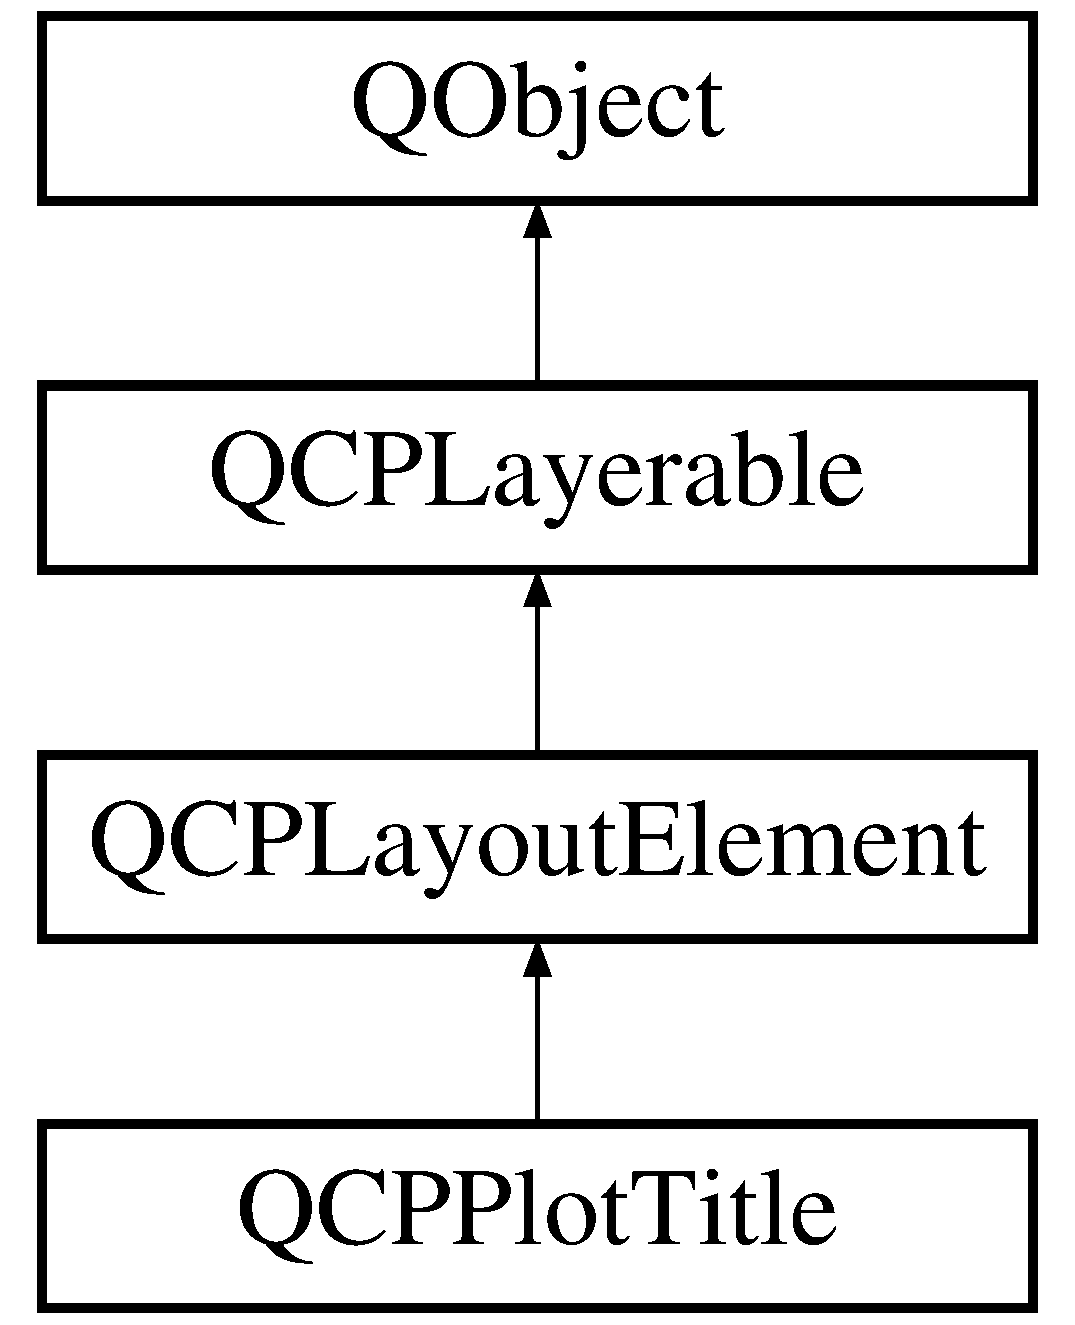
\includegraphics[height=4.000000cm]{class_q_c_p_plot_title}
\end{center}
\end{figure}
\subsection*{Signals}
\begin{DoxyCompactItemize}
\item 
void \hyperlink{class_q_c_p_plot_title_a3a01ede2da3b0b5eda33aa5274cc3523}{selection\+Changed} (bool selected)
\item 
\hypertarget{class_q_c_p_plot_title_a5eac3c17a4dbabb75250bc1210a83cfc}{}\label{class_q_c_p_plot_title_a5eac3c17a4dbabb75250bc1210a83cfc} 
void {\bfseries selectable\+Changed} (bool selectable)
\end{DoxyCompactItemize}
\subsection*{Public Member Functions}
\begin{DoxyCompactItemize}
\item 
\hyperlink{class_q_c_p_plot_title_aaae17bee2de6d6a1e695f76fb1abed03}{Q\+C\+P\+Plot\+Title} (\hyperlink{class_q_custom_plot}{Q\+Custom\+Plot} $\ast$parent\+Plot)
\item 
\hyperlink{class_q_c_p_plot_title_a90b9f46ceccbeee41f71c895a8c7ee1f}{Q\+C\+P\+Plot\+Title} (\hyperlink{class_q_custom_plot}{Q\+Custom\+Plot} $\ast$parent\+Plot, const Q\+String \&text)
\item 
\hypertarget{class_q_c_p_plot_title_ab1d6bdf3ce3548a745ae921e7453e2ae}{}\label{class_q_c_p_plot_title_ab1d6bdf3ce3548a745ae921e7453e2ae} 
Q\+String {\bfseries text} () const
\item 
\hypertarget{class_q_c_p_plot_title_a28711580ab9d488c134dbf5d5e68e150}{}\label{class_q_c_p_plot_title_a28711580ab9d488c134dbf5d5e68e150} 
Q\+Font {\bfseries font} () const
\item 
\hypertarget{class_q_c_p_plot_title_a1fa7af5df28f6bfc99e4f6be65c51ff4}{}\label{class_q_c_p_plot_title_a1fa7af5df28f6bfc99e4f6be65c51ff4} 
Q\+Color {\bfseries text\+Color} () const
\item 
\hypertarget{class_q_c_p_plot_title_a3a801cc8af4b892e8f7571dae8b990dc}{}\label{class_q_c_p_plot_title_a3a801cc8af4b892e8f7571dae8b990dc} 
Q\+Font {\bfseries selected\+Font} () const
\item 
\hypertarget{class_q_c_p_plot_title_ac811f7305f28200b2a515e69c2932938}{}\label{class_q_c_p_plot_title_ac811f7305f28200b2a515e69c2932938} 
Q\+Color {\bfseries selected\+Text\+Color} () const
\item 
\hypertarget{class_q_c_p_plot_title_ab53d1140b1e34e6cd10fdd084eb38417}{}\label{class_q_c_p_plot_title_ab53d1140b1e34e6cd10fdd084eb38417} 
bool {\bfseries selectable} () const
\item 
\hypertarget{class_q_c_p_plot_title_a60c91808dbd29640429549947a38f191}{}\label{class_q_c_p_plot_title_a60c91808dbd29640429549947a38f191} 
bool {\bfseries selected} () const
\item 
void \hyperlink{class_q_c_p_plot_title_aae5a93e88050dfb2cbf6adc087516821}{set\+Text} (const Q\+String \&text)
\item 
void \hyperlink{class_q_c_p_plot_title_a199fc7170802ea65006c371875349e37}{set\+Font} (const Q\+Font \&font)
\item 
void \hyperlink{class_q_c_p_plot_title_a71273e3a0ca6b4c151591b37b9e5ce33}{set\+Text\+Color} (const Q\+Color \&color)
\item 
void \hyperlink{class_q_c_p_plot_title_a5245980ead999ceed51dbe702d0e3131}{set\+Selected\+Font} (const Q\+Font \&font)
\item 
void \hyperlink{class_q_c_p_plot_title_a09ffd8c52ac8824d00382f84be391b66}{set\+Selected\+Text\+Color} (const Q\+Color \&color)
\item 
Q\+\_\+\+S\+L\+OT void \hyperlink{class_q_c_p_plot_title_a8866b07b9fa14877d4cefbf38406c5dd}{set\+Selectable} (bool selectable)
\item 
Q\+\_\+\+S\+L\+OT void \hyperlink{class_q_c_p_plot_title_a8d441a889d371307df86f1ab7687a333}{set\+Selected} (bool selected)
\item 
virtual double \hyperlink{class_q_c_p_plot_title_aae4bcb2401e6947ea0abd3c960488d35}{select\+Test} (const Q\+PointF \&pos, bool only\+Selectable, Q\+Variant $\ast$details=0) const
\end{DoxyCompactItemize}
\subsection*{Protected Member Functions}
\begin{DoxyCompactItemize}
\item 
\hypertarget{class_q_c_p_plot_title_ae225a89ab1f62e8a364e01f12c13c4d3}{}\label{class_q_c_p_plot_title_ae225a89ab1f62e8a364e01f12c13c4d3} 
virtual void {\bfseries apply\+Default\+Antialiasing\+Hint} (\hyperlink{class_q_c_p_painter}{Q\+C\+P\+Painter} $\ast$painter) const
\item 
\hypertarget{class_q_c_p_plot_title_ae4f1f8d24489628dabb7256363b097d2}{}\label{class_q_c_p_plot_title_ae4f1f8d24489628dabb7256363b097d2} 
virtual void {\bfseries draw} (\hyperlink{class_q_c_p_painter}{Q\+C\+P\+Painter} $\ast$painter)
\item 
virtual Q\+Size \hyperlink{class_q_c_p_plot_title_aeed5454134516655723bf2d0499dea24}{minimum\+Size\+Hint} () const
\item 
virtual Q\+Size \hyperlink{class_q_c_p_plot_title_ae24c395b5d3be64b42dcb9e27ed023c4}{maximum\+Size\+Hint} () const
\item 
\hypertarget{class_q_c_p_plot_title_a22672ef2abe442b1e73b7ee04cff9bdd}{}\label{class_q_c_p_plot_title_a22672ef2abe442b1e73b7ee04cff9bdd} 
virtual void {\bfseries select\+Event} (Q\+Mouse\+Event $\ast$event, bool additive, const Q\+Variant \&details, bool $\ast$selection\+State\+Changed)
\item 
\hypertarget{class_q_c_p_plot_title_ac6dfce05bebdb9bd0bfacd5ff02f3325}{}\label{class_q_c_p_plot_title_ac6dfce05bebdb9bd0bfacd5ff02f3325} 
virtual void {\bfseries deselect\+Event} (bool $\ast$selection\+State\+Changed)
\item 
\hypertarget{class_q_c_p_plot_title_a581b0215a6b16e5995b2f7e3bd4febb9}{}\label{class_q_c_p_plot_title_a581b0215a6b16e5995b2f7e3bd4febb9} 
Q\+Font {\bfseries main\+Font} () const
\item 
\hypertarget{class_q_c_p_plot_title_aaff84f2291e654faf84419c370fa50cf}{}\label{class_q_c_p_plot_title_aaff84f2291e654faf84419c370fa50cf} 
Q\+Color {\bfseries main\+Text\+Color} () const
\end{DoxyCompactItemize}
\subsection*{Protected Attributes}
\begin{DoxyCompactItemize}
\item 
\hypertarget{class_q_c_p_plot_title_a0d961bfac1211d59d3b0bc30d35f6379}{}\label{class_q_c_p_plot_title_a0d961bfac1211d59d3b0bc30d35f6379} 
Q\+String {\bfseries m\+Text}
\item 
\hypertarget{class_q_c_p_plot_title_ad9e2c2a2e941f3444cb692a51df0df62}{}\label{class_q_c_p_plot_title_ad9e2c2a2e941f3444cb692a51df0df62} 
Q\+Font {\bfseries m\+Font}
\item 
\hypertarget{class_q_c_p_plot_title_a5d7f834d6522c1a72fb0682c0b7ebe13}{}\label{class_q_c_p_plot_title_a5d7f834d6522c1a72fb0682c0b7ebe13} 
Q\+Color {\bfseries m\+Text\+Color}
\item 
\hypertarget{class_q_c_p_plot_title_a95003186c39bbab902873a8ef4cbb547}{}\label{class_q_c_p_plot_title_a95003186c39bbab902873a8ef4cbb547} 
Q\+Font {\bfseries m\+Selected\+Font}
\item 
\hypertarget{class_q_c_p_plot_title_a8b9760e62af92814c4effdd7ad69c5f9}{}\label{class_q_c_p_plot_title_a8b9760e62af92814c4effdd7ad69c5f9} 
Q\+Color {\bfseries m\+Selected\+Text\+Color}
\item 
\hypertarget{class_q_c_p_plot_title_a7178a0f6c1e633c144c17b4de4e0b840}{}\label{class_q_c_p_plot_title_a7178a0f6c1e633c144c17b4de4e0b840} 
Q\+Rect {\bfseries m\+Text\+Bounding\+Rect}
\item 
\hypertarget{class_q_c_p_plot_title_aadefb5e2b19b1cc7deda0a55ec747884}{}\label{class_q_c_p_plot_title_aadefb5e2b19b1cc7deda0a55ec747884} 
bool {\bfseries m\+Selectable}
\item 
\hypertarget{class_q_c_p_plot_title_afef1342a20f5ca985a20b9cfdc03d815}{}\label{class_q_c_p_plot_title_afef1342a20f5ca985a20b9cfdc03d815} 
bool {\bfseries m\+Selected}
\end{DoxyCompactItemize}
\subsection*{Additional Inherited Members}


\subsection{Detailed Description}
A layout element displaying a plot title text. 

The text may be specified with \hyperlink{class_q_c_p_plot_title_aae5a93e88050dfb2cbf6adc087516821}{set\+Text}, theformatting can be controlled with \hyperlink{class_q_c_p_plot_title_a199fc7170802ea65006c371875349e37}{set\+Font} and \hyperlink{class_q_c_p_plot_title_a71273e3a0ca6b4c151591b37b9e5ce33}{set\+Text\+Color}.

A plot title can be added as follows\+: 
\begin{DoxyCodeInclude}
\end{DoxyCodeInclude}
 Since a plot title is a common requirement, \hyperlink{class_q_custom_plot}{Q\+Custom\+Plot} offers specialized selection signals for easy interaction with \hyperlink{class_q_c_p_plot_title}{Q\+C\+P\+Plot\+Title}. If a layout element of type \hyperlink{class_q_c_p_plot_title}{Q\+C\+P\+Plot\+Title} is clicked, the signal \hyperlink{class_q_custom_plot_a2137a819e518fee7edd1c0bf5984d8d6}{Q\+Custom\+Plot\+::title\+Click} is emitted. A double click emits the \hyperlink{class_q_custom_plot_ad51d65f6abf5edfaeef6e0519a4c1a2f}{Q\+Custom\+Plot\+::title\+Double\+Click} signal. 

\subsection{Constructor \& Destructor Documentation}
\hypertarget{class_q_c_p_plot_title_aaae17bee2de6d6a1e695f76fb1abed03}{}\label{class_q_c_p_plot_title_aaae17bee2de6d6a1e695f76fb1abed03} 
\index{Q\+C\+P\+Plot\+Title@{Q\+C\+P\+Plot\+Title}!Q\+C\+P\+Plot\+Title@{Q\+C\+P\+Plot\+Title}}
\index{Q\+C\+P\+Plot\+Title@{Q\+C\+P\+Plot\+Title}!Q\+C\+P\+Plot\+Title@{Q\+C\+P\+Plot\+Title}}
\subsubsection{\texorpdfstring{Q\+C\+P\+Plot\+Title()}{QCPPlotTitle()}\hspace{0.1cm}{\footnotesize\ttfamily [1/2]}}
{\footnotesize\ttfamily Q\+C\+P\+Plot\+Title\+::\+Q\+C\+P\+Plot\+Title (\begin{DoxyParamCaption}\item[{\hyperlink{class_q_custom_plot}{Q\+Custom\+Plot} $\ast$}]{parent\+Plot }\end{DoxyParamCaption})\hspace{0.3cm}{\ttfamily [explicit]}}

Creates a new \hyperlink{class_q_c_p_plot_title}{Q\+C\+P\+Plot\+Title} instance and sets default values. The initial text is empty (\hyperlink{class_q_c_p_plot_title_aae5a93e88050dfb2cbf6adc087516821}{set\+Text}).

To set the title text in the constructor, rather use \hyperlink{class_q_c_p_plot_title_a90b9f46ceccbeee41f71c895a8c7ee1f}{Q\+C\+P\+Plot\+Title(\+Q\+Custom\+Plot $\ast$parent\+Plot, const Q\+String \&text)}. \hypertarget{class_q_c_p_plot_title_a90b9f46ceccbeee41f71c895a8c7ee1f}{}\label{class_q_c_p_plot_title_a90b9f46ceccbeee41f71c895a8c7ee1f} 
\index{Q\+C\+P\+Plot\+Title@{Q\+C\+P\+Plot\+Title}!Q\+C\+P\+Plot\+Title@{Q\+C\+P\+Plot\+Title}}
\index{Q\+C\+P\+Plot\+Title@{Q\+C\+P\+Plot\+Title}!Q\+C\+P\+Plot\+Title@{Q\+C\+P\+Plot\+Title}}
\subsubsection{\texorpdfstring{Q\+C\+P\+Plot\+Title()}{QCPPlotTitle()}\hspace{0.1cm}{\footnotesize\ttfamily [2/2]}}
{\footnotesize\ttfamily Q\+C\+P\+Plot\+Title\+::\+Q\+C\+P\+Plot\+Title (\begin{DoxyParamCaption}\item[{\hyperlink{class_q_custom_plot}{Q\+Custom\+Plot} $\ast$}]{parent\+Plot,  }\item[{const Q\+String \&}]{text }\end{DoxyParamCaption})\hspace{0.3cm}{\ttfamily [explicit]}}

This is an overloaded member function, provided for convenience. It differs from the above function only in what argument(s) it accepts.

Creates a new \hyperlink{class_q_c_p_plot_title}{Q\+C\+P\+Plot\+Title} instance and sets default values. The initial text is set to {\itshape text}. 

\subsection{Member Function Documentation}
\hypertarget{class_q_c_p_plot_title_ae24c395b5d3be64b42dcb9e27ed023c4}{}\label{class_q_c_p_plot_title_ae24c395b5d3be64b42dcb9e27ed023c4} 
\index{Q\+C\+P\+Plot\+Title@{Q\+C\+P\+Plot\+Title}!maximum\+Size\+Hint@{maximum\+Size\+Hint}}
\index{maximum\+Size\+Hint@{maximum\+Size\+Hint}!Q\+C\+P\+Plot\+Title@{Q\+C\+P\+Plot\+Title}}
\subsubsection{\texorpdfstring{maximum\+Size\+Hint()}{maximumSizeHint()}}
{\footnotesize\ttfamily Q\+Size Q\+C\+P\+Plot\+Title\+::maximum\+Size\+Hint (\begin{DoxyParamCaption}{ }\end{DoxyParamCaption}) const\hspace{0.3cm}{\ttfamily [protected]}, {\ttfamily [virtual]}}

Returns the maximum size this layout element (the inner \hyperlink{class_q_c_p_layout_element_a208effccfe2cca4a0eaf9393e60f2dd4}{rect}) may be expanded to.

if a maximum size (\hyperlink{class_q_c_p_layout_element_a74eb5280a737ab44833d506db65efd95}{set\+Maximum\+Size}) was not set manually, parent layouts consult this function to determine the maximum allowed size of this layout element. (A manual maximum size is considered set if it is smaller than Qt\textquotesingle{}s Q\+W\+I\+D\+G\+E\+T\+S\+I\+Z\+E\+\_\+\+M\+AX.) 

Reimplemented from \hyperlink{class_q_c_p_layout_element_ab5ce2ba22b36d9a3b70a1be562c326e5}{Q\+C\+P\+Layout\+Element}.

\hypertarget{class_q_c_p_plot_title_aeed5454134516655723bf2d0499dea24}{}\label{class_q_c_p_plot_title_aeed5454134516655723bf2d0499dea24} 
\index{Q\+C\+P\+Plot\+Title@{Q\+C\+P\+Plot\+Title}!minimum\+Size\+Hint@{minimum\+Size\+Hint}}
\index{minimum\+Size\+Hint@{minimum\+Size\+Hint}!Q\+C\+P\+Plot\+Title@{Q\+C\+P\+Plot\+Title}}
\subsubsection{\texorpdfstring{minimum\+Size\+Hint()}{minimumSizeHint()}}
{\footnotesize\ttfamily Q\+Size Q\+C\+P\+Plot\+Title\+::minimum\+Size\+Hint (\begin{DoxyParamCaption}{ }\end{DoxyParamCaption}) const\hspace{0.3cm}{\ttfamily [protected]}, {\ttfamily [virtual]}}

Returns the minimum size this layout element (the inner \hyperlink{class_q_c_p_layout_element_a208effccfe2cca4a0eaf9393e60f2dd4}{rect}) may be compressed to.

if a minimum size (\hyperlink{class_q_c_p_layout_element_a5dd29a3c8bc88440c97c06b67be7886b}{set\+Minimum\+Size}) was not set manually, parent layouts consult this function to determine the minimum allowed size of this layout element. (A manual minimum size is considered set if it is non-\/zero.) 

Reimplemented from \hyperlink{class_q_c_p_layout_element_ab3fdb5c9a5189bb2dac10d4d25329cd8}{Q\+C\+P\+Layout\+Element}.

\hypertarget{class_q_c_p_plot_title_a3a01ede2da3b0b5eda33aa5274cc3523}{}\label{class_q_c_p_plot_title_a3a01ede2da3b0b5eda33aa5274cc3523} 
\index{Q\+C\+P\+Plot\+Title@{Q\+C\+P\+Plot\+Title}!selection\+Changed@{selection\+Changed}}
\index{selection\+Changed@{selection\+Changed}!Q\+C\+P\+Plot\+Title@{Q\+C\+P\+Plot\+Title}}
\subsubsection{\texorpdfstring{selection\+Changed}{selectionChanged}}
{\footnotesize\ttfamily void Q\+C\+P\+Plot\+Title\+::selection\+Changed (\begin{DoxyParamCaption}\item[{bool}]{selected }\end{DoxyParamCaption})\hspace{0.3cm}{\ttfamily [signal]}}

This signal is emitted when the selection state has changed to {\itshape selected}, either by user interaction or by a direct call to \hyperlink{class_q_c_p_plot_title_a8d441a889d371307df86f1ab7687a333}{set\+Selected}.

\begin{DoxySeeAlso}{See also}
\hyperlink{class_q_c_p_plot_title_a8d441a889d371307df86f1ab7687a333}{set\+Selected}, \hyperlink{class_q_c_p_plot_title_a8866b07b9fa14877d4cefbf38406c5dd}{set\+Selectable} 
\end{DoxySeeAlso}
\hypertarget{class_q_c_p_plot_title_aae4bcb2401e6947ea0abd3c960488d35}{}\label{class_q_c_p_plot_title_aae4bcb2401e6947ea0abd3c960488d35} 
\index{Q\+C\+P\+Plot\+Title@{Q\+C\+P\+Plot\+Title}!select\+Test@{select\+Test}}
\index{select\+Test@{select\+Test}!Q\+C\+P\+Plot\+Title@{Q\+C\+P\+Plot\+Title}}
\subsubsection{\texorpdfstring{select\+Test()}{selectTest()}}
{\footnotesize\ttfamily double Q\+C\+P\+Plot\+Title\+::select\+Test (\begin{DoxyParamCaption}\item[{const Q\+PointF \&}]{pos,  }\item[{bool}]{only\+Selectable,  }\item[{Q\+Variant $\ast$}]{details = {\ttfamily 0} }\end{DoxyParamCaption}) const\hspace{0.3cm}{\ttfamily [virtual]}}

Layout elements are sensitive to events inside their outer rect. If {\itshape pos} is within the outer rect, this method returns a value corresponding to 0.\+99 times the parent plot\textquotesingle{}s selection tolerance. However, layout elements are not selectable by default. So if {\itshape only\+Selectable} is true, -\/1.\+0 is returned.

See \hyperlink{class_q_c_p_layerable_a04db8351fefd44cfdb77958e75c6288e}{Q\+C\+P\+Layerable\+::select\+Test} for a general explanation of this virtual method.

\hyperlink{class_q_c_p_layout_element}{Q\+C\+P\+Layout\+Element} subclasses may reimplement this method to provide more specific selection test behaviour. 

Reimplemented from \hyperlink{class_q_c_p_layout_element_a0b96ae0d7bcfa6e38188fcb1e73e143f}{Q\+C\+P\+Layout\+Element}.

\hypertarget{class_q_c_p_plot_title_a199fc7170802ea65006c371875349e37}{}\label{class_q_c_p_plot_title_a199fc7170802ea65006c371875349e37} 
\index{Q\+C\+P\+Plot\+Title@{Q\+C\+P\+Plot\+Title}!set\+Font@{set\+Font}}
\index{set\+Font@{set\+Font}!Q\+C\+P\+Plot\+Title@{Q\+C\+P\+Plot\+Title}}
\subsubsection{\texorpdfstring{set\+Font()}{setFont()}}
{\footnotesize\ttfamily void Q\+C\+P\+Plot\+Title\+::set\+Font (\begin{DoxyParamCaption}\item[{const Q\+Font \&}]{font }\end{DoxyParamCaption})}

Sets the {\itshape font} of the title text.

\begin{DoxySeeAlso}{See also}
\hyperlink{class_q_c_p_plot_title_a71273e3a0ca6b4c151591b37b9e5ce33}{set\+Text\+Color}, \hyperlink{class_q_c_p_plot_title_a5245980ead999ceed51dbe702d0e3131}{set\+Selected\+Font} 
\end{DoxySeeAlso}
\hypertarget{class_q_c_p_plot_title_a8866b07b9fa14877d4cefbf38406c5dd}{}\label{class_q_c_p_plot_title_a8866b07b9fa14877d4cefbf38406c5dd} 
\index{Q\+C\+P\+Plot\+Title@{Q\+C\+P\+Plot\+Title}!set\+Selectable@{set\+Selectable}}
\index{set\+Selectable@{set\+Selectable}!Q\+C\+P\+Plot\+Title@{Q\+C\+P\+Plot\+Title}}
\subsubsection{\texorpdfstring{set\+Selectable()}{setSelectable()}}
{\footnotesize\ttfamily void Q\+C\+P\+Plot\+Title\+::set\+Selectable (\begin{DoxyParamCaption}\item[{bool}]{selectable }\end{DoxyParamCaption})}

Sets whether the user may select this plot title to {\itshape selectable}.

Note that even when {\itshape selectable} is set to {\ttfamily false}, the selection state may be changed programmatically via \hyperlink{class_q_c_p_plot_title_a8d441a889d371307df86f1ab7687a333}{set\+Selected}. \hypertarget{class_q_c_p_plot_title_a8d441a889d371307df86f1ab7687a333}{}\label{class_q_c_p_plot_title_a8d441a889d371307df86f1ab7687a333} 
\index{Q\+C\+P\+Plot\+Title@{Q\+C\+P\+Plot\+Title}!set\+Selected@{set\+Selected}}
\index{set\+Selected@{set\+Selected}!Q\+C\+P\+Plot\+Title@{Q\+C\+P\+Plot\+Title}}
\subsubsection{\texorpdfstring{set\+Selected()}{setSelected()}}
{\footnotesize\ttfamily void Q\+C\+P\+Plot\+Title\+::set\+Selected (\begin{DoxyParamCaption}\item[{bool}]{selected }\end{DoxyParamCaption})}

Sets the selection state of this plot title to {\itshape selected}. If the selection has changed, \hyperlink{class_q_c_p_plot_title_a3a01ede2da3b0b5eda33aa5274cc3523}{selection\+Changed} is emitted.

Note that this function can change the selection state independently of the current \hyperlink{class_q_c_p_plot_title_a8866b07b9fa14877d4cefbf38406c5dd}{set\+Selectable} state. \hypertarget{class_q_c_p_plot_title_a5245980ead999ceed51dbe702d0e3131}{}\label{class_q_c_p_plot_title_a5245980ead999ceed51dbe702d0e3131} 
\index{Q\+C\+P\+Plot\+Title@{Q\+C\+P\+Plot\+Title}!set\+Selected\+Font@{set\+Selected\+Font}}
\index{set\+Selected\+Font@{set\+Selected\+Font}!Q\+C\+P\+Plot\+Title@{Q\+C\+P\+Plot\+Title}}
\subsubsection{\texorpdfstring{set\+Selected\+Font()}{setSelectedFont()}}
{\footnotesize\ttfamily void Q\+C\+P\+Plot\+Title\+::set\+Selected\+Font (\begin{DoxyParamCaption}\item[{const Q\+Font \&}]{font }\end{DoxyParamCaption})}

Sets the {\itshape font} of the title text that will be used if the plot title is selected (\hyperlink{class_q_c_p_plot_title_a8d441a889d371307df86f1ab7687a333}{set\+Selected}).

\begin{DoxySeeAlso}{See also}
\hyperlink{class_q_c_p_plot_title_a199fc7170802ea65006c371875349e37}{set\+Font} 
\end{DoxySeeAlso}
\hypertarget{class_q_c_p_plot_title_a09ffd8c52ac8824d00382f84be391b66}{}\label{class_q_c_p_plot_title_a09ffd8c52ac8824d00382f84be391b66} 
\index{Q\+C\+P\+Plot\+Title@{Q\+C\+P\+Plot\+Title}!set\+Selected\+Text\+Color@{set\+Selected\+Text\+Color}}
\index{set\+Selected\+Text\+Color@{set\+Selected\+Text\+Color}!Q\+C\+P\+Plot\+Title@{Q\+C\+P\+Plot\+Title}}
\subsubsection{\texorpdfstring{set\+Selected\+Text\+Color()}{setSelectedTextColor()}}
{\footnotesize\ttfamily void Q\+C\+P\+Plot\+Title\+::set\+Selected\+Text\+Color (\begin{DoxyParamCaption}\item[{const Q\+Color \&}]{color }\end{DoxyParamCaption})}

Sets the {\itshape color} of the title text that will be used if the plot title is selected (\hyperlink{class_q_c_p_plot_title_a8d441a889d371307df86f1ab7687a333}{set\+Selected}).

\begin{DoxySeeAlso}{See also}
\hyperlink{class_q_c_p_plot_title_a71273e3a0ca6b4c151591b37b9e5ce33}{set\+Text\+Color} 
\end{DoxySeeAlso}
\hypertarget{class_q_c_p_plot_title_aae5a93e88050dfb2cbf6adc087516821}{}\label{class_q_c_p_plot_title_aae5a93e88050dfb2cbf6adc087516821} 
\index{Q\+C\+P\+Plot\+Title@{Q\+C\+P\+Plot\+Title}!set\+Text@{set\+Text}}
\index{set\+Text@{set\+Text}!Q\+C\+P\+Plot\+Title@{Q\+C\+P\+Plot\+Title}}
\subsubsection{\texorpdfstring{set\+Text()}{setText()}}
{\footnotesize\ttfamily void Q\+C\+P\+Plot\+Title\+::set\+Text (\begin{DoxyParamCaption}\item[{const Q\+String \&}]{text }\end{DoxyParamCaption})}

Sets the text that will be displayed to {\itshape text}. Multiple lines can be created by insertion of \char`\"{}\textbackslash{}n\char`\"{}.

\begin{DoxySeeAlso}{See also}
\hyperlink{class_q_c_p_plot_title_a199fc7170802ea65006c371875349e37}{set\+Font}, \hyperlink{class_q_c_p_plot_title_a71273e3a0ca6b4c151591b37b9e5ce33}{set\+Text\+Color} 
\end{DoxySeeAlso}
\hypertarget{class_q_c_p_plot_title_a71273e3a0ca6b4c151591b37b9e5ce33}{}\label{class_q_c_p_plot_title_a71273e3a0ca6b4c151591b37b9e5ce33} 
\index{Q\+C\+P\+Plot\+Title@{Q\+C\+P\+Plot\+Title}!set\+Text\+Color@{set\+Text\+Color}}
\index{set\+Text\+Color@{set\+Text\+Color}!Q\+C\+P\+Plot\+Title@{Q\+C\+P\+Plot\+Title}}
\subsubsection{\texorpdfstring{set\+Text\+Color()}{setTextColor()}}
{\footnotesize\ttfamily void Q\+C\+P\+Plot\+Title\+::set\+Text\+Color (\begin{DoxyParamCaption}\item[{const Q\+Color \&}]{color }\end{DoxyParamCaption})}

Sets the {\itshape color} of the title text.

\begin{DoxySeeAlso}{See also}
\hyperlink{class_q_c_p_plot_title_a199fc7170802ea65006c371875349e37}{set\+Font}, \hyperlink{class_q_c_p_plot_title_a09ffd8c52ac8824d00382f84be391b66}{set\+Selected\+Text\+Color} 
\end{DoxySeeAlso}


The documentation for this class was generated from the following files\+:\begin{DoxyCompactItemize}
\item 
F\+E\+S\+S-\/\+G\+U\+I/\hyperlink{qcustomplot_8h}{qcustomplot.\+h}\item 
F\+E\+S\+S-\/\+G\+U\+I/\hyperlink{qcustomplot_8cpp}{qcustomplot.\+cpp}\end{DoxyCompactItemize}

\hypertarget{class_q_c_p_range}{}\section{Q\+C\+P\+Range Class Reference}
\label{class_q_c_p_range}\index{Q\+C\+P\+Range@{Q\+C\+P\+Range}}


Represents the range an axis is encompassing.  


\subsection*{Public Member Functions}
\begin{DoxyCompactItemize}
\item 
\hyperlink{class_q_c_p_range_aca158d7e69702cee5d77d10a269b01e2}{Q\+C\+P\+Range} ()
\item 
\hyperlink{class_q_c_p_range_a1d9d84d084c8f368fdedd42e0978d405}{Q\+C\+P\+Range} (double lower, double upper)
\item 
\hypertarget{class_q_c_p_range_a9f8d1fdcf4b6d19779f1c3d9a14b09c9}{}\label{class_q_c_p_range_a9f8d1fdcf4b6d19779f1c3d9a14b09c9} 
bool {\bfseries operator==} (const \hyperlink{class_q_c_p_range}{Q\+C\+P\+Range} \&other) const
\item 
\hypertarget{class_q_c_p_range_a4827a37c83b8bb4bf53fcf8f6a257e77}{}\label{class_q_c_p_range_a4827a37c83b8bb4bf53fcf8f6a257e77} 
bool {\bfseries operator!=} (const \hyperlink{class_q_c_p_range}{Q\+C\+P\+Range} \&other) const
\item 
\hyperlink{class_q_c_p_range}{Q\+C\+P\+Range} \& \hyperlink{class_q_c_p_range_afea7c1aa7d08f061cd9bd8832f957df8}{operator+=} (const double \&value)
\item 
\hyperlink{class_q_c_p_range}{Q\+C\+P\+Range} \& \hyperlink{class_q_c_p_range_a95894bcb15a16a75ca564091374e2191}{operator-\/=} (const double \&value)
\item 
\hyperlink{class_q_c_p_range}{Q\+C\+P\+Range} \& \hyperlink{class_q_c_p_range_a6876aa9620ff2f0f7f1873f998372cef}{operator$\ast$=} (const double \&value)
\item 
\hyperlink{class_q_c_p_range}{Q\+C\+P\+Range} \& \hyperlink{class_q_c_p_range_a6137d8682b6835ace840730b4c1e2d63}{operator/=} (const double \&value)
\item 
double \hyperlink{class_q_c_p_range_a62326e7cc4316b96df6a60813230e63f}{size} () const
\item 
double \hyperlink{class_q_c_p_range_af57d4a37a45d0101177ca30fae5d4ca8}{center} () const
\item 
void \hyperlink{class_q_c_p_range_af914a7740269b0604d0827c634a878a9}{normalize} ()
\item 
void \hyperlink{class_q_c_p_range_a0fa1bc8048be50d52bea93a8caf08305}{expand} (const \hyperlink{class_q_c_p_range}{Q\+C\+P\+Range} \&other\+Range)
\item 
\hyperlink{class_q_c_p_range}{Q\+C\+P\+Range} \hyperlink{class_q_c_p_range_a9cbfb7cd06eac1839cae981e05c19633}{expanded} (const \hyperlink{class_q_c_p_range}{Q\+C\+P\+Range} \&other\+Range) const
\item 
\hyperlink{class_q_c_p_range}{Q\+C\+P\+Range} \hyperlink{class_q_c_p_range_a3d66288d66e1d6df3636075eb42502ee}{sanitized\+For\+Log\+Scale} () const
\item 
\hyperlink{class_q_c_p_range}{Q\+C\+P\+Range} \hyperlink{class_q_c_p_range_a808751fdd9b17ef52327ba011df2e5f1}{sanitized\+For\+Lin\+Scale} () const
\item 
bool \hyperlink{class_q_c_p_range_ae9842b48b6d38dc5e9607358e3083cc8}{contains} (double value) const
\end{DoxyCompactItemize}
\subsection*{Static Public Member Functions}
\begin{DoxyCompactItemize}
\item 
static bool \hyperlink{class_q_c_p_range_ab38bd4841c77c7bb86c9eea0f142dcc0}{valid\+Range} (double lower, double upper)
\item 
static bool \hyperlink{class_q_c_p_range_a801b964752eaad6219be9d8a651ec2b3}{valid\+Range} (const \hyperlink{class_q_c_p_range}{Q\+C\+P\+Range} \&range)
\end{DoxyCompactItemize}
\subsection*{Public Attributes}
\begin{DoxyCompactItemize}
\item 
\hypertarget{class_q_c_p_range_aa3aca3edb14f7ca0c85d912647b91745}{}\label{class_q_c_p_range_aa3aca3edb14f7ca0c85d912647b91745} 
double {\bfseries lower}
\item 
\hypertarget{class_q_c_p_range_ae44eb3aafe1d0e2ed34b499b6d2e074f}{}\label{class_q_c_p_range_ae44eb3aafe1d0e2ed34b499b6d2e074f} 
double {\bfseries upper}
\end{DoxyCompactItemize}
\subsection*{Static Public Attributes}
\begin{DoxyCompactItemize}
\item 
static const double \hyperlink{class_q_c_p_range_ab46d3bc95030ee25efda41b89e2b616b}{min\+Range} = 1e-\/280
\item 
static const double \hyperlink{class_q_c_p_range_a5ca51e7a2dc5dc0d49527ab171fe1f4f}{max\+Range} = 1e250
\end{DoxyCompactItemize}
\subsection*{Friends}
\begin{DoxyCompactItemize}
\item 
const \hyperlink{class_q_c_p_range}{Q\+C\+P\+Range} \hyperlink{class_q_c_p_range_af53ea6fb823a4a5897162b865841de04}{operator+} (const \hyperlink{class_q_c_p_range}{Q\+C\+P\+Range} \&, double)
\item 
const \hyperlink{class_q_c_p_range}{Q\+C\+P\+Range} \hyperlink{class_q_c_p_range_a9fb2e9941d32001482df670c0d704977}{operator+} (double, const \hyperlink{class_q_c_p_range}{Q\+C\+P\+Range} \&)
\item 
const \hyperlink{class_q_c_p_range}{Q\+C\+P\+Range} \hyperlink{class_q_c_p_range_a797f82830b516646da8873f82e39e356}{operator-\/} (const \hyperlink{class_q_c_p_range}{Q\+C\+P\+Range} \&range, double value)
\item 
const \hyperlink{class_q_c_p_range}{Q\+C\+P\+Range} \hyperlink{class_q_c_p_range_a558b1248ff6a9e41fd5b2630555a8acc}{operator$\ast$} (const \hyperlink{class_q_c_p_range}{Q\+C\+P\+Range} \&range, double value)
\item 
const \hyperlink{class_q_c_p_range}{Q\+C\+P\+Range} \hyperlink{class_q_c_p_range_a5cb2332f6957021f47cc768089f4f090}{operator$\ast$} (double value, const \hyperlink{class_q_c_p_range}{Q\+C\+P\+Range} \&range)
\item 
const \hyperlink{class_q_c_p_range}{Q\+C\+P\+Range} \hyperlink{class_q_c_p_range_a4b366a3a21974c88e09b0d39d4a24a4b}{operator/} (const \hyperlink{class_q_c_p_range}{Q\+C\+P\+Range} \&range, double value)
\end{DoxyCompactItemize}


\subsection{Detailed Description}
Represents the range an axis is encompassing. 

contains a {\itshape lower} and {\itshape upper} double value and provides convenience input, output and modification functions.

\begin{DoxySeeAlso}{See also}
\hyperlink{class_q_c_p_axis_aebdfea5d44c3a0ad2b4700cd4d25b641}{Q\+C\+P\+Axis\+::set\+Range} 
\end{DoxySeeAlso}


\subsection{Constructor \& Destructor Documentation}
\hypertarget{class_q_c_p_range_aca158d7e69702cee5d77d10a269b01e2}{}\label{class_q_c_p_range_aca158d7e69702cee5d77d10a269b01e2} 
\index{Q\+C\+P\+Range@{Q\+C\+P\+Range}!Q\+C\+P\+Range@{Q\+C\+P\+Range}}
\index{Q\+C\+P\+Range@{Q\+C\+P\+Range}!Q\+C\+P\+Range@{Q\+C\+P\+Range}}
\subsubsection{\texorpdfstring{Q\+C\+P\+Range()}{QCPRange()}\hspace{0.1cm}{\footnotesize\ttfamily [1/2]}}
{\footnotesize\ttfamily Q\+C\+P\+Range\+::\+Q\+C\+P\+Range (\begin{DoxyParamCaption}{ }\end{DoxyParamCaption})}

Constructs a range with {\itshape lower} and {\itshape upper} set to zero. \hypertarget{class_q_c_p_range_a1d9d84d084c8f368fdedd42e0978d405}{}\label{class_q_c_p_range_a1d9d84d084c8f368fdedd42e0978d405} 
\index{Q\+C\+P\+Range@{Q\+C\+P\+Range}!Q\+C\+P\+Range@{Q\+C\+P\+Range}}
\index{Q\+C\+P\+Range@{Q\+C\+P\+Range}!Q\+C\+P\+Range@{Q\+C\+P\+Range}}
\subsubsection{\texorpdfstring{Q\+C\+P\+Range()}{QCPRange()}\hspace{0.1cm}{\footnotesize\ttfamily [2/2]}}
{\footnotesize\ttfamily Q\+C\+P\+Range\+::\+Q\+C\+P\+Range (\begin{DoxyParamCaption}\item[{double}]{lower,  }\item[{double}]{upper }\end{DoxyParamCaption})}

This is an overloaded member function, provided for convenience. It differs from the above function only in what argument(s) it accepts. Constructs a range with the specified {\itshape lower} and {\itshape upper} values. 

\subsection{Member Function Documentation}
\hypertarget{class_q_c_p_range_af57d4a37a45d0101177ca30fae5d4ca8}{}\label{class_q_c_p_range_af57d4a37a45d0101177ca30fae5d4ca8} 
\index{Q\+C\+P\+Range@{Q\+C\+P\+Range}!center@{center}}
\index{center@{center}!Q\+C\+P\+Range@{Q\+C\+P\+Range}}
\subsubsection{\texorpdfstring{center()}{center()}}
{\footnotesize\ttfamily double Q\+C\+P\+Range\+::center (\begin{DoxyParamCaption}{ }\end{DoxyParamCaption}) const}

Returns the center of the range, i.\+e. ({\itshape upper+{\itshape lower})$\ast$0}.5 \hypertarget{class_q_c_p_range_ae9842b48b6d38dc5e9607358e3083cc8}{}\label{class_q_c_p_range_ae9842b48b6d38dc5e9607358e3083cc8} 
\index{Q\+C\+P\+Range@{Q\+C\+P\+Range}!contains@{contains}}
\index{contains@{contains}!Q\+C\+P\+Range@{Q\+C\+P\+Range}}
\subsubsection{\texorpdfstring{contains()}{contains()}}
{\footnotesize\ttfamily bool Q\+C\+P\+Range\+::contains (\begin{DoxyParamCaption}\item[{double}]{value }\end{DoxyParamCaption}) const}

Returns true when {\itshape value} lies within or exactly on the borders of the range. \hypertarget{class_q_c_p_range_a0fa1bc8048be50d52bea93a8caf08305}{}\label{class_q_c_p_range_a0fa1bc8048be50d52bea93a8caf08305} 
\index{Q\+C\+P\+Range@{Q\+C\+P\+Range}!expand@{expand}}
\index{expand@{expand}!Q\+C\+P\+Range@{Q\+C\+P\+Range}}
\subsubsection{\texorpdfstring{expand()}{expand()}}
{\footnotesize\ttfamily void Q\+C\+P\+Range\+::expand (\begin{DoxyParamCaption}\item[{const \hyperlink{class_q_c_p_range}{Q\+C\+P\+Range} \&}]{other\+Range }\end{DoxyParamCaption})}

Expands this range such that {\itshape other\+Range} is contained in the new range. It is assumed that both this range and {\itshape other\+Range} are normalized (see \hyperlink{class_q_c_p_range_af914a7740269b0604d0827c634a878a9}{normalize}).

If {\itshape other\+Range} is already inside the current range, this function does nothing.

\begin{DoxySeeAlso}{See also}
\hyperlink{class_q_c_p_range_a9cbfb7cd06eac1839cae981e05c19633}{expanded} 
\end{DoxySeeAlso}
\hypertarget{class_q_c_p_range_a9cbfb7cd06eac1839cae981e05c19633}{}\label{class_q_c_p_range_a9cbfb7cd06eac1839cae981e05c19633} 
\index{Q\+C\+P\+Range@{Q\+C\+P\+Range}!expanded@{expanded}}
\index{expanded@{expanded}!Q\+C\+P\+Range@{Q\+C\+P\+Range}}
\subsubsection{\texorpdfstring{expanded()}{expanded()}}
{\footnotesize\ttfamily \hyperlink{class_q_c_p_range}{Q\+C\+P\+Range} Q\+C\+P\+Range\+::expanded (\begin{DoxyParamCaption}\item[{const \hyperlink{class_q_c_p_range}{Q\+C\+P\+Range} \&}]{other\+Range }\end{DoxyParamCaption}) const}

Returns an expanded range that contains this and {\itshape other\+Range}. It is assumed that both this range and {\itshape other\+Range} are normalized (see \hyperlink{class_q_c_p_range_af914a7740269b0604d0827c634a878a9}{normalize}).

\begin{DoxySeeAlso}{See also}
\hyperlink{class_q_c_p_range_a0fa1bc8048be50d52bea93a8caf08305}{expand} 
\end{DoxySeeAlso}
\hypertarget{class_q_c_p_range_af914a7740269b0604d0827c634a878a9}{}\label{class_q_c_p_range_af914a7740269b0604d0827c634a878a9} 
\index{Q\+C\+P\+Range@{Q\+C\+P\+Range}!normalize@{normalize}}
\index{normalize@{normalize}!Q\+C\+P\+Range@{Q\+C\+P\+Range}}
\subsubsection{\texorpdfstring{normalize()}{normalize()}}
{\footnotesize\ttfamily void Q\+C\+P\+Range\+::normalize (\begin{DoxyParamCaption}{ }\end{DoxyParamCaption})}

Makes sure {\itshape lower} is numerically smaller than {\itshape upper}. If this is not the case, the values are swapped. \hypertarget{class_q_c_p_range_a6876aa9620ff2f0f7f1873f998372cef}{}\label{class_q_c_p_range_a6876aa9620ff2f0f7f1873f998372cef} 
\index{Q\+C\+P\+Range@{Q\+C\+P\+Range}!operator$\ast$=@{operator$\ast$=}}
\index{operator$\ast$=@{operator$\ast$=}!Q\+C\+P\+Range@{Q\+C\+P\+Range}}
\subsubsection{\texorpdfstring{operator$\ast$=()}{operator*=()}}
{\footnotesize\ttfamily \hyperlink{class_q_c_p_range}{Q\+C\+P\+Range} \& Q\+C\+P\+Range\+::operator$\ast$= (\begin{DoxyParamCaption}\item[{const double \&}]{value }\end{DoxyParamCaption})\hspace{0.3cm}{\ttfamily [inline]}}

Multiplies both boundaries of the range by {\itshape value}. \hypertarget{class_q_c_p_range_afea7c1aa7d08f061cd9bd8832f957df8}{}\label{class_q_c_p_range_afea7c1aa7d08f061cd9bd8832f957df8} 
\index{Q\+C\+P\+Range@{Q\+C\+P\+Range}!operator+=@{operator+=}}
\index{operator+=@{operator+=}!Q\+C\+P\+Range@{Q\+C\+P\+Range}}
\subsubsection{\texorpdfstring{operator+=()}{operator+=()}}
{\footnotesize\ttfamily \hyperlink{class_q_c_p_range}{Q\+C\+P\+Range} \& Q\+C\+P\+Range\+::operator+= (\begin{DoxyParamCaption}\item[{const double \&}]{value }\end{DoxyParamCaption})\hspace{0.3cm}{\ttfamily [inline]}}

Adds {\itshape value} to both boundaries of the range. \hypertarget{class_q_c_p_range_a95894bcb15a16a75ca564091374e2191}{}\label{class_q_c_p_range_a95894bcb15a16a75ca564091374e2191} 
\index{Q\+C\+P\+Range@{Q\+C\+P\+Range}!operator-\/=@{operator-\/=}}
\index{operator-\/=@{operator-\/=}!Q\+C\+P\+Range@{Q\+C\+P\+Range}}
\subsubsection{\texorpdfstring{operator-\/=()}{operator-=()}}
{\footnotesize\ttfamily \hyperlink{class_q_c_p_range}{Q\+C\+P\+Range} \& Q\+C\+P\+Range\+::operator-\/= (\begin{DoxyParamCaption}\item[{const double \&}]{value }\end{DoxyParamCaption})\hspace{0.3cm}{\ttfamily [inline]}}

Subtracts {\itshape value} from both boundaries of the range. \hypertarget{class_q_c_p_range_a6137d8682b6835ace840730b4c1e2d63}{}\label{class_q_c_p_range_a6137d8682b6835ace840730b4c1e2d63} 
\index{Q\+C\+P\+Range@{Q\+C\+P\+Range}!operator/=@{operator/=}}
\index{operator/=@{operator/=}!Q\+C\+P\+Range@{Q\+C\+P\+Range}}
\subsubsection{\texorpdfstring{operator/=()}{operator/=()}}
{\footnotesize\ttfamily \hyperlink{class_q_c_p_range}{Q\+C\+P\+Range} \& Q\+C\+P\+Range\+::operator/= (\begin{DoxyParamCaption}\item[{const double \&}]{value }\end{DoxyParamCaption})\hspace{0.3cm}{\ttfamily [inline]}}

Divides both boundaries of the range by {\itshape value}. \hypertarget{class_q_c_p_range_a808751fdd9b17ef52327ba011df2e5f1}{}\label{class_q_c_p_range_a808751fdd9b17ef52327ba011df2e5f1} 
\index{Q\+C\+P\+Range@{Q\+C\+P\+Range}!sanitized\+For\+Lin\+Scale@{sanitized\+For\+Lin\+Scale}}
\index{sanitized\+For\+Lin\+Scale@{sanitized\+For\+Lin\+Scale}!Q\+C\+P\+Range@{Q\+C\+P\+Range}}
\subsubsection{\texorpdfstring{sanitized\+For\+Lin\+Scale()}{sanitizedForLinScale()}}
{\footnotesize\ttfamily \hyperlink{class_q_c_p_range}{Q\+C\+P\+Range} Q\+C\+P\+Range\+::sanitized\+For\+Lin\+Scale (\begin{DoxyParamCaption}{ }\end{DoxyParamCaption}) const}

Returns a sanitized version of the range. Sanitized means for linear scales, that {\itshape lower} will always be numerically smaller (or equal) to {\itshape upper}. \hypertarget{class_q_c_p_range_a3d66288d66e1d6df3636075eb42502ee}{}\label{class_q_c_p_range_a3d66288d66e1d6df3636075eb42502ee} 
\index{Q\+C\+P\+Range@{Q\+C\+P\+Range}!sanitized\+For\+Log\+Scale@{sanitized\+For\+Log\+Scale}}
\index{sanitized\+For\+Log\+Scale@{sanitized\+For\+Log\+Scale}!Q\+C\+P\+Range@{Q\+C\+P\+Range}}
\subsubsection{\texorpdfstring{sanitized\+For\+Log\+Scale()}{sanitizedForLogScale()}}
{\footnotesize\ttfamily \hyperlink{class_q_c_p_range}{Q\+C\+P\+Range} Q\+C\+P\+Range\+::sanitized\+For\+Log\+Scale (\begin{DoxyParamCaption}{ }\end{DoxyParamCaption}) const}

Returns a sanitized version of the range. Sanitized means for logarithmic scales, that the range won\textquotesingle{}t span the positive and negative sign domain, i.\+e. contain zero. Further {\itshape lower} will always be numerically smaller (or equal) to {\itshape upper}.

If the original range does span positive and negative sign domains or contains zero, the returned range will try to approximate the original range as good as possible. If the positive interval of the original range is wider than the negative interval, the returned range will only contain the positive interval, with lower bound set to {\itshape range\+Fac} or {\itshape range\+Fac} $\ast${\itshape upper}, whichever is closer to zero. Same procedure is used if the negative interval is wider than the positive interval, this time by changing the {\itshape upper} bound. \hypertarget{class_q_c_p_range_a62326e7cc4316b96df6a60813230e63f}{}\label{class_q_c_p_range_a62326e7cc4316b96df6a60813230e63f} 
\index{Q\+C\+P\+Range@{Q\+C\+P\+Range}!size@{size}}
\index{size@{size}!Q\+C\+P\+Range@{Q\+C\+P\+Range}}
\subsubsection{\texorpdfstring{size()}{size()}}
{\footnotesize\ttfamily double Q\+C\+P\+Range\+::size (\begin{DoxyParamCaption}{ }\end{DoxyParamCaption}) const}

Returns the size of the range, i.\+e. {\itshape upper-\/{\itshape lower} } \hypertarget{class_q_c_p_range_ab38bd4841c77c7bb86c9eea0f142dcc0}{}\label{class_q_c_p_range_ab38bd4841c77c7bb86c9eea0f142dcc0} 
\index{Q\+C\+P\+Range@{Q\+C\+P\+Range}!valid\+Range@{valid\+Range}}
\index{valid\+Range@{valid\+Range}!Q\+C\+P\+Range@{Q\+C\+P\+Range}}
\subsubsection{\texorpdfstring{valid\+Range()}{validRange()}\hspace{0.1cm}{\footnotesize\ttfamily [1/2]}}
{\footnotesize\ttfamily bool Q\+C\+P\+Range\+::valid\+Range (\begin{DoxyParamCaption}\item[{double}]{lower,  }\item[{double}]{upper }\end{DoxyParamCaption})\hspace{0.3cm}{\ttfamily [static]}}

Checks, whether the specified range is within valid bounds, which are defined as \hyperlink{class_q_c_p_range_a5ca51e7a2dc5dc0d49527ab171fe1f4f}{Q\+C\+P\+Range\+::max\+Range} and \hyperlink{class_q_c_p_range_ab46d3bc95030ee25efda41b89e2b616b}{Q\+C\+P\+Range\+::min\+Range}. A valid range means\+: \begin{DoxyItemize}
\item range bounds within -\/max\+Range and max\+Range \item range size above min\+Range \item range size below max\+Range \end{DoxyItemize}
\hypertarget{class_q_c_p_range_a801b964752eaad6219be9d8a651ec2b3}{}\label{class_q_c_p_range_a801b964752eaad6219be9d8a651ec2b3} 
\index{Q\+C\+P\+Range@{Q\+C\+P\+Range}!valid\+Range@{valid\+Range}}
\index{valid\+Range@{valid\+Range}!Q\+C\+P\+Range@{Q\+C\+P\+Range}}
\subsubsection{\texorpdfstring{valid\+Range()}{validRange()}\hspace{0.1cm}{\footnotesize\ttfamily [2/2]}}
{\footnotesize\ttfamily bool Q\+C\+P\+Range\+::valid\+Range (\begin{DoxyParamCaption}\item[{const \hyperlink{class_q_c_p_range}{Q\+C\+P\+Range} \&}]{range }\end{DoxyParamCaption})\hspace{0.3cm}{\ttfamily [static]}}

This is an overloaded member function, provided for convenience. It differs from the above function only in what argument(s) it accepts. Checks, whether the specified range is within valid bounds, which are defined as \hyperlink{class_q_c_p_range_a5ca51e7a2dc5dc0d49527ab171fe1f4f}{Q\+C\+P\+Range\+::max\+Range} and \hyperlink{class_q_c_p_range_ab46d3bc95030ee25efda41b89e2b616b}{Q\+C\+P\+Range\+::min\+Range}. A valid range means\+: \begin{DoxyItemize}
\item range bounds within -\/max\+Range and max\+Range \item range size above min\+Range \item range size below max\+Range \end{DoxyItemize}


\subsection{Friends And Related Function Documentation}
\hypertarget{class_q_c_p_range_a558b1248ff6a9e41fd5b2630555a8acc}{}\label{class_q_c_p_range_a558b1248ff6a9e41fd5b2630555a8acc} 
\index{Q\+C\+P\+Range@{Q\+C\+P\+Range}!operator$\ast$@{operator$\ast$}}
\index{operator$\ast$@{operator$\ast$}!Q\+C\+P\+Range@{Q\+C\+P\+Range}}
\subsubsection{\texorpdfstring{operator$\ast$}{operator*}\hspace{0.1cm}{\footnotesize\ttfamily [1/2]}}
{\footnotesize\ttfamily const \hyperlink{class_q_c_p_range}{Q\+C\+P\+Range} operator$\ast$ (\begin{DoxyParamCaption}\item[{const \hyperlink{class_q_c_p_range}{Q\+C\+P\+Range} \&}]{range,  }\item[{double}]{value }\end{DoxyParamCaption})\hspace{0.3cm}{\ttfamily [friend]}}

Multiplies both boundaries of the range by {\itshape value}. \hypertarget{class_q_c_p_range_a5cb2332f6957021f47cc768089f4f090}{}\label{class_q_c_p_range_a5cb2332f6957021f47cc768089f4f090} 
\index{Q\+C\+P\+Range@{Q\+C\+P\+Range}!operator$\ast$@{operator$\ast$}}
\index{operator$\ast$@{operator$\ast$}!Q\+C\+P\+Range@{Q\+C\+P\+Range}}
\subsubsection{\texorpdfstring{operator$\ast$}{operator*}\hspace{0.1cm}{\footnotesize\ttfamily [2/2]}}
{\footnotesize\ttfamily const \hyperlink{class_q_c_p_range}{Q\+C\+P\+Range} operator$\ast$ (\begin{DoxyParamCaption}\item[{double}]{value,  }\item[{const \hyperlink{class_q_c_p_range}{Q\+C\+P\+Range} \&}]{range }\end{DoxyParamCaption})\hspace{0.3cm}{\ttfamily [friend]}}

Multiplies both boundaries of the range by {\itshape value}. \hypertarget{class_q_c_p_range_af53ea6fb823a4a5897162b865841de04}{}\label{class_q_c_p_range_af53ea6fb823a4a5897162b865841de04} 
\index{Q\+C\+P\+Range@{Q\+C\+P\+Range}!operator+@{operator+}}
\index{operator+@{operator+}!Q\+C\+P\+Range@{Q\+C\+P\+Range}}
\subsubsection{\texorpdfstring{operator+}{operator+}\hspace{0.1cm}{\footnotesize\ttfamily [1/2]}}
{\footnotesize\ttfamily const \hyperlink{class_q_c_p_range}{Q\+C\+P\+Range} operator+ (\begin{DoxyParamCaption}\item[{const \hyperlink{class_q_c_p_range}{Q\+C\+P\+Range} \&}]{range,  }\item[{double}]{value }\end{DoxyParamCaption})\hspace{0.3cm}{\ttfamily [friend]}}

Adds {\itshape value} to both boundaries of the range. \hypertarget{class_q_c_p_range_a9fb2e9941d32001482df670c0d704977}{}\label{class_q_c_p_range_a9fb2e9941d32001482df670c0d704977} 
\index{Q\+C\+P\+Range@{Q\+C\+P\+Range}!operator+@{operator+}}
\index{operator+@{operator+}!Q\+C\+P\+Range@{Q\+C\+P\+Range}}
\subsubsection{\texorpdfstring{operator+}{operator+}\hspace{0.1cm}{\footnotesize\ttfamily [2/2]}}
{\footnotesize\ttfamily const \hyperlink{class_q_c_p_range}{Q\+C\+P\+Range} operator+ (\begin{DoxyParamCaption}\item[{double}]{value,  }\item[{const \hyperlink{class_q_c_p_range}{Q\+C\+P\+Range} \&}]{range }\end{DoxyParamCaption})\hspace{0.3cm}{\ttfamily [friend]}}

Adds {\itshape value} to both boundaries of the range. \hypertarget{class_q_c_p_range_a797f82830b516646da8873f82e39e356}{}\label{class_q_c_p_range_a797f82830b516646da8873f82e39e356} 
\index{Q\+C\+P\+Range@{Q\+C\+P\+Range}!operator-\/@{operator-\/}}
\index{operator-\/@{operator-\/}!Q\+C\+P\+Range@{Q\+C\+P\+Range}}
\subsubsection{\texorpdfstring{operator-\/}{operator-}}
{\footnotesize\ttfamily const \hyperlink{class_q_c_p_range}{Q\+C\+P\+Range} operator-\/ (\begin{DoxyParamCaption}\item[{const \hyperlink{class_q_c_p_range}{Q\+C\+P\+Range} \&}]{range,  }\item[{double}]{value }\end{DoxyParamCaption})\hspace{0.3cm}{\ttfamily [friend]}}

Subtracts {\itshape value} from both boundaries of the range. \hypertarget{class_q_c_p_range_a4b366a3a21974c88e09b0d39d4a24a4b}{}\label{class_q_c_p_range_a4b366a3a21974c88e09b0d39d4a24a4b} 
\index{Q\+C\+P\+Range@{Q\+C\+P\+Range}!operator/@{operator/}}
\index{operator/@{operator/}!Q\+C\+P\+Range@{Q\+C\+P\+Range}}
\subsubsection{\texorpdfstring{operator/}{operator/}}
{\footnotesize\ttfamily const \hyperlink{class_q_c_p_range}{Q\+C\+P\+Range} operator/ (\begin{DoxyParamCaption}\item[{const \hyperlink{class_q_c_p_range}{Q\+C\+P\+Range} \&}]{range,  }\item[{double}]{value }\end{DoxyParamCaption})\hspace{0.3cm}{\ttfamily [friend]}}

Divides both boundaries of the range by {\itshape value}. 

\subsection{Member Data Documentation}
\hypertarget{class_q_c_p_range_a5ca51e7a2dc5dc0d49527ab171fe1f4f}{}\label{class_q_c_p_range_a5ca51e7a2dc5dc0d49527ab171fe1f4f} 
\index{Q\+C\+P\+Range@{Q\+C\+P\+Range}!max\+Range@{max\+Range}}
\index{max\+Range@{max\+Range}!Q\+C\+P\+Range@{Q\+C\+P\+Range}}
\subsubsection{\texorpdfstring{max\+Range}{maxRange}}
{\footnotesize\ttfamily const double Q\+C\+P\+Range\+::max\+Range = 1e250\hspace{0.3cm}{\ttfamily [static]}}

Maximum values (negative and positive) the range will accept in range-\/changing functions. Larger absolute values would cause errors due to the 11-\/bit exponent of double precision numbers, corresponding to a maximum magnitude of roughly 1e308. Since the number of planck-\/volumes in the entire visible universe is only $\sim$1e183, this should be enough. \begin{DoxySeeAlso}{See also}
\hyperlink{class_q_c_p_range_ab38bd4841c77c7bb86c9eea0f142dcc0}{valid\+Range}, \hyperlink{class_q_c_p_range_ab46d3bc95030ee25efda41b89e2b616b}{min\+Range} 
\end{DoxySeeAlso}
\hypertarget{class_q_c_p_range_ab46d3bc95030ee25efda41b89e2b616b}{}\label{class_q_c_p_range_ab46d3bc95030ee25efda41b89e2b616b} 
\index{Q\+C\+P\+Range@{Q\+C\+P\+Range}!min\+Range@{min\+Range}}
\index{min\+Range@{min\+Range}!Q\+C\+P\+Range@{Q\+C\+P\+Range}}
\subsubsection{\texorpdfstring{min\+Range}{minRange}}
{\footnotesize\ttfamily const double Q\+C\+P\+Range\+::min\+Range = 1e-\/280\hspace{0.3cm}{\ttfamily [static]}}

Minimum range size ({\itshape upper} -\/ {\itshape lower}) the range changing functions will accept. Smaller intervals would cause errors due to the 11-\/bit exponent of double precision numbers, corresponding to a minimum magnitude of roughly 1e-\/308. \begin{DoxySeeAlso}{See also}
\hyperlink{class_q_c_p_range_ab38bd4841c77c7bb86c9eea0f142dcc0}{valid\+Range}, \hyperlink{class_q_c_p_range_a5ca51e7a2dc5dc0d49527ab171fe1f4f}{max\+Range} 
\end{DoxySeeAlso}


The documentation for this class was generated from the following files\+:\begin{DoxyCompactItemize}
\item 
F\+E\+S\+S-\/\+G\+U\+I/\hyperlink{qcustomplot_8h}{qcustomplot.\+h}\item 
F\+E\+S\+S-\/\+G\+U\+I/\hyperlink{qcustomplot_8cpp}{qcustomplot.\+cpp}\end{DoxyCompactItemize}

\hypertarget{class_q_c_p_scatter_style}{}\section{Q\+C\+P\+Scatter\+Style Class Reference}
\label{class_q_c_p_scatter_style}\index{Q\+C\+P\+Scatter\+Style@{Q\+C\+P\+Scatter\+Style}}


Represents the visual appearance of scatter points.  


\subsection*{Public Types}
\begin{DoxyCompactItemize}
\item 
enum \hyperlink{class_q_c_p_scatter_style_adb31525af6b680e6f1b7472e43859349}{Scatter\+Shape} \{ \newline
\hyperlink{class_q_c_p_scatter_style_adb31525af6b680e6f1b7472e43859349abd144c291ca274f77053ec68cab6c022}{ss\+None}, 
\hyperlink{class_q_c_p_scatter_style_adb31525af6b680e6f1b7472e43859349a06e15a735b79093a1d999c0374fa3aa1}{ss\+Dot}, 
\hyperlink{class_q_c_p_scatter_style_adb31525af6b680e6f1b7472e43859349a9eacd60f059dc3ef71bf249f515a6fe4}{ss\+Cross}, 
\hyperlink{class_q_c_p_scatter_style_adb31525af6b680e6f1b7472e43859349a2d7f1d3c1a148b9d9d17f2fd9cae5eb7}{ss\+Plus}, 
\newline
\hyperlink{class_q_c_p_scatter_style_adb31525af6b680e6f1b7472e43859349a7c92a110880d0ef2170dff3a5b4f7779}{ss\+Circle}, 
\hyperlink{class_q_c_p_scatter_style_adb31525af6b680e6f1b7472e43859349a281fe1434696dcbab3aa6b9ccfbb09e9}{ss\+Disc}, 
\hyperlink{class_q_c_p_scatter_style_adb31525af6b680e6f1b7472e43859349a279e48703ddc9f1cf4a61d3e2817ab3c}{ss\+Square}, 
\hyperlink{class_q_c_p_scatter_style_adb31525af6b680e6f1b7472e43859349a4fc5929df1b2dad0a3cb2ef2c8b6e633}{ss\+Diamond}, 
\newline
\hyperlink{class_q_c_p_scatter_style_adb31525af6b680e6f1b7472e43859349a6047a2d64e41f1d6ce54445d595d442f}{ss\+Star}, 
\hyperlink{class_q_c_p_scatter_style_adb31525af6b680e6f1b7472e43859349a74a8d4eff1d97b57c53a60d0003453c3}{ss\+Triangle}, 
\hyperlink{class_q_c_p_scatter_style_adb31525af6b680e6f1b7472e43859349a6156274d21d8b4115197567d3ea2d9a8}{ss\+Triangle\+Inverted}, 
\hyperlink{class_q_c_p_scatter_style_adb31525af6b680e6f1b7472e43859349a7081310936c200c6c78e34c172f72d07}{ss\+Cross\+Square}, 
\newline
\hyperlink{class_q_c_p_scatter_style_adb31525af6b680e6f1b7472e43859349a5aa8e9db545e5404482fec774768ee25}{ss\+Plus\+Square}, 
\hyperlink{class_q_c_p_scatter_style_adb31525af6b680e6f1b7472e43859349a524613ba5d1c4eaa1541d74cf339d283}{ss\+Cross\+Circle}, 
\hyperlink{class_q_c_p_scatter_style_adb31525af6b680e6f1b7472e43859349a6fa151d01f1694c9ff9922da686dc535}{ss\+Plus\+Circle}, 
\hyperlink{class_q_c_p_scatter_style_adb31525af6b680e6f1b7472e43859349ada3b2988ece38c121922a4b5007eb08d}{ss\+Peace}, 
\newline
\hyperlink{class_q_c_p_scatter_style_adb31525af6b680e6f1b7472e43859349a8718b849ca7c307b07b8e091efb0c31e}{ss\+Pixmap}, 
\hyperlink{class_q_c_p_scatter_style_adb31525af6b680e6f1b7472e43859349a15d9bcfd9de94edda949006529f9219d}{ss\+Custom}
 \}
\end{DoxyCompactItemize}
\subsection*{Public Member Functions}
\begin{DoxyCompactItemize}
\item 
\hyperlink{class_q_c_p_scatter_style_a8836018d9ad83ccd8870de8315c1be73}{Q\+C\+P\+Scatter\+Style} ()
\item 
\hyperlink{class_q_c_p_scatter_style_a003d92f74f4561eda111862eadd62f28}{Q\+C\+P\+Scatter\+Style} (\hyperlink{class_q_c_p_scatter_style_adb31525af6b680e6f1b7472e43859349}{Scatter\+Shape} shape, double size=6)
\item 
\hyperlink{class_q_c_p_scatter_style_afa059da858c864c7e05871dc602d7eab}{Q\+C\+P\+Scatter\+Style} (\hyperlink{class_q_c_p_scatter_style_adb31525af6b680e6f1b7472e43859349}{Scatter\+Shape} shape, const Q\+Color \&color, double size)
\item 
\hyperlink{class_q_c_p_scatter_style_a6e1b64f12cac7f07af180ae4316fd38d}{Q\+C\+P\+Scatter\+Style} (\hyperlink{class_q_c_p_scatter_style_adb31525af6b680e6f1b7472e43859349}{Scatter\+Shape} shape, const Q\+Color \&color, const Q\+Color \&fill, double size)
\item 
\hyperlink{class_q_c_p_scatter_style_a85acc4941d7e5c9bca5fa51377a77f49}{Q\+C\+P\+Scatter\+Style} (\hyperlink{class_q_c_p_scatter_style_adb31525af6b680e6f1b7472e43859349}{Scatter\+Shape} shape, const Q\+Pen \&pen, const Q\+Brush \&brush, double size)
\item 
\hyperlink{class_q_c_p_scatter_style_a63962094587a4c2258435aa7933996cc}{Q\+C\+P\+Scatter\+Style} (const Q\+Pixmap \&pixmap)
\item 
\hyperlink{class_q_c_p_scatter_style_a879c30647683b3cfbde2afecea815e6f}{Q\+C\+P\+Scatter\+Style} (const Q\+Painter\+Path \&custom\+Path, const Q\+Pen \&pen, const Q\+Brush \&brush=Qt\+::\+No\+Brush, double size=6)
\item 
\hypertarget{class_q_c_p_scatter_style_a0e94526d9165d9f50e262102bdd71a47}{}\label{class_q_c_p_scatter_style_a0e94526d9165d9f50e262102bdd71a47} 
double {\bfseries size} () const
\item 
\hypertarget{class_q_c_p_scatter_style_af04cad55bd7f58a96da4fc6bc46a0a1e}{}\label{class_q_c_p_scatter_style_af04cad55bd7f58a96da4fc6bc46a0a1e} 
\hyperlink{class_q_c_p_scatter_style_adb31525af6b680e6f1b7472e43859349}{Scatter\+Shape} {\bfseries shape} () const
\item 
\hypertarget{class_q_c_p_scatter_style_acdd6313d16e69d3810e9d1f48dd9e4bb}{}\label{class_q_c_p_scatter_style_acdd6313d16e69d3810e9d1f48dd9e4bb} 
Q\+Pen {\bfseries pen} () const
\item 
\hypertarget{class_q_c_p_scatter_style_adc4f66aed84f1d7a3a5aabf4f48f31a6}{}\label{class_q_c_p_scatter_style_adc4f66aed84f1d7a3a5aabf4f48f31a6} 
Q\+Brush {\bfseries brush} () const
\item 
\hypertarget{class_q_c_p_scatter_style_a9b2d1a2ec0aac0c74f7582d14050e93a}{}\label{class_q_c_p_scatter_style_a9b2d1a2ec0aac0c74f7582d14050e93a} 
Q\+Pixmap {\bfseries pixmap} () const
\item 
\hypertarget{class_q_c_p_scatter_style_aef1fac84c9830fd97f2a8568e605e372}{}\label{class_q_c_p_scatter_style_aef1fac84c9830fd97f2a8568e605e372} 
Q\+Painter\+Path {\bfseries custom\+Path} () const
\item 
void \hyperlink{class_q_c_p_scatter_style_aaefdd031052892c4136129db68596e0f}{set\+Size} (double size)
\item 
void \hyperlink{class_q_c_p_scatter_style_a7c641c4d4c6d29cb705d3887cfce91c1}{set\+Shape} (\hyperlink{class_q_c_p_scatter_style_adb31525af6b680e6f1b7472e43859349}{Scatter\+Shape} shape)
\item 
void \hyperlink{class_q_c_p_scatter_style_a761f1f229cc0ca4703e1e2b89f6dd1ba}{set\+Pen} (const Q\+Pen \&pen)
\item 
void \hyperlink{class_q_c_p_scatter_style_a74d692aaeb8d4b36d6f7d510e44264b1}{set\+Brush} (const Q\+Brush \&brush)
\item 
void \hyperlink{class_q_c_p_scatter_style_a5fb611d46acfac520d7b89a1c71d9246}{set\+Pixmap} (const Q\+Pixmap \&pixmap)
\item 
void \hyperlink{class_q_c_p_scatter_style_a96a3e949f90b2afe5677ca9412a12a1e}{set\+Custom\+Path} (const Q\+Painter\+Path \&custom\+Path)
\item 
bool \hyperlink{class_q_c_p_scatter_style_a72db6bcb1e1abd6e53c1315dd3dea7e4}{is\+None} () const
\item 
bool \hyperlink{class_q_c_p_scatter_style_a47077eb6450fe9a788f833e4ec1b1d5a}{is\+Pen\+Defined} () const
\item 
void \hyperlink{class_q_c_p_scatter_style_afd8044ece445300499ca0dc164821e0f}{apply\+To} (\hyperlink{class_q_c_p_painter}{Q\+C\+P\+Painter} $\ast$painter, const Q\+Pen \&default\+Pen) const
\item 
void \hyperlink{class_q_c_p_scatter_style_a2b3964961b6cbfbc87be6e1e3a6f3c96}{draw\+Shape} (\hyperlink{class_q_c_p_painter}{Q\+C\+P\+Painter} $\ast$painter, Q\+PointF pos) const
\item 
void \hyperlink{class_q_c_p_scatter_style_a95c297b114c77c22428ef40f54620ddf}{draw\+Shape} (\hyperlink{class_q_c_p_painter}{Q\+C\+P\+Painter} $\ast$painter, double x, double y) const
\end{DoxyCompactItemize}
\subsection*{Protected Attributes}
\begin{DoxyCompactItemize}
\item 
\hypertarget{class_q_c_p_scatter_style_a757da98671eb06b221979373ac2cec91}{}\label{class_q_c_p_scatter_style_a757da98671eb06b221979373ac2cec91} 
double {\bfseries m\+Size}
\item 
\hypertarget{class_q_c_p_scatter_style_af1b327f35f107ed108290187bbc8c7c6}{}\label{class_q_c_p_scatter_style_af1b327f35f107ed108290187bbc8c7c6} 
\hyperlink{class_q_c_p_scatter_style_adb31525af6b680e6f1b7472e43859349}{Scatter\+Shape} {\bfseries m\+Shape}
\item 
\hypertarget{class_q_c_p_scatter_style_a0f6a85e6d1e3ae1ca1b6efb4d4cdfe17}{}\label{class_q_c_p_scatter_style_a0f6a85e6d1e3ae1ca1b6efb4d4cdfe17} 
Q\+Pen {\bfseries m\+Pen}
\item 
\hypertarget{class_q_c_p_scatter_style_a1b9c6ab10aebcaf236f1f45d1d6d64d1}{}\label{class_q_c_p_scatter_style_a1b9c6ab10aebcaf236f1f45d1d6d64d1} 
Q\+Brush {\bfseries m\+Brush}
\item 
\hypertarget{class_q_c_p_scatter_style_a7697346c89b19d4cd1d8dd33319ec9e3}{}\label{class_q_c_p_scatter_style_a7697346c89b19d4cd1d8dd33319ec9e3} 
Q\+Pixmap {\bfseries m\+Pixmap}
\item 
\hypertarget{class_q_c_p_scatter_style_a813cb074744dc5a2f59cc99d6a10c6f0}{}\label{class_q_c_p_scatter_style_a813cb074744dc5a2f59cc99d6a10c6f0} 
Q\+Painter\+Path {\bfseries m\+Custom\+Path}
\item 
\hypertarget{class_q_c_p_scatter_style_a84ef5aa591ddba07b440f597e1669e78}{}\label{class_q_c_p_scatter_style_a84ef5aa591ddba07b440f597e1669e78} 
bool {\bfseries m\+Pen\+Defined}
\end{DoxyCompactItemize}


\subsection{Detailed Description}
Represents the visual appearance of scatter points. 

This class holds information about shape, color and size of scatter points. In plottables like \hyperlink{class_q_c_p_graph}{Q\+C\+P\+Graph} it is used to store how scatter points shall be drawn. For example, \hyperlink{class_q_c_p_graph_a12bd17a8ba21983163ec5d8f42a9fea5}{Q\+C\+P\+Graph\+::set\+Scatter\+Style} takes a \hyperlink{class_q_c_p_scatter_style}{Q\+C\+P\+Scatter\+Style} instance.

A scatter style consists of a shape (\hyperlink{class_q_c_p_scatter_style_a7c641c4d4c6d29cb705d3887cfce91c1}{set\+Shape}), a line color (\hyperlink{class_q_c_p_scatter_style_a761f1f229cc0ca4703e1e2b89f6dd1ba}{set\+Pen}) and possibly a fill (\hyperlink{class_q_c_p_scatter_style_a74d692aaeb8d4b36d6f7d510e44264b1}{set\+Brush}), if the shape provides a fillable area. Further, the size of the shape can be controlled with \hyperlink{class_q_c_p_scatter_style_aaefdd031052892c4136129db68596e0f}{set\+Size}.\hypertarget{class_q_c_p_scatter_style_QCPScatterStyle-defining}{}\subsection{Specifying a scatter style}\label{class_q_c_p_scatter_style_QCPScatterStyle-defining}
You can set all these configurations either by calling the respective functions on an instance\+: 
\begin{DoxyCodeInclude}
\end{DoxyCodeInclude}
 Or you can use one of the various constructors that take different parameter combinations, making it easy to specify a scatter style in a single call, like so\+: 
\begin{DoxyCodeInclude}
\end{DoxyCodeInclude}
 \hypertarget{class_q_c_p_scatter_style_QCPScatterStyle-undefinedpen}{}\subsection{Leaving the color/pen up to the plottable}\label{class_q_c_p_scatter_style_QCPScatterStyle-undefinedpen}
There are two constructors which leave the pen undefined\+: \hyperlink{class_q_c_p_scatter_style_a8836018d9ad83ccd8870de8315c1be73}{Q\+C\+P\+Scatter\+Style()} and \hyperlink{class_q_c_p_scatter_style_a003d92f74f4561eda111862eadd62f28}{Q\+C\+P\+Scatter\+Style(\+Scatter\+Shape shape, double size)}. If those constructors are used, a call to \hyperlink{class_q_c_p_scatter_style_a47077eb6450fe9a788f833e4ec1b1d5a}{is\+Pen\+Defined} will return false. It leads to scatter points that inherit the pen from the plottable that uses the scatter style. Thus, if such a scatter style is passed to \hyperlink{class_q_c_p_graph}{Q\+C\+P\+Graph}, the line color of the graph (\hyperlink{class_q_c_p_abstract_plottable_ab74b09ae4c0e7e13142fe4b5bf46cac7}{Q\+C\+P\+Graph\+::set\+Pen}) will be used by the scatter points. This makes it very convenient to set up typical scatter settings\+:


\begin{DoxyCodeInclude}
\end{DoxyCodeInclude}
 Notice that it wasn\textquotesingle{}t even necessary to explicitly call a \hyperlink{class_q_c_p_scatter_style}{Q\+C\+P\+Scatter\+Style} constructor. This works because \hyperlink{class_q_c_p_scatter_style}{Q\+C\+P\+Scatter\+Style} provides a constructor that can transform a \hyperlink{class_q_c_p_scatter_style_adb31525af6b680e6f1b7472e43859349}{Scatter\+Shape} directly into a \hyperlink{class_q_c_p_scatter_style}{Q\+C\+P\+Scatter\+Style} instance (that\textquotesingle{}s the \hyperlink{class_q_c_p_scatter_style_a003d92f74f4561eda111862eadd62f28}{Q\+C\+P\+Scatter\+Style(\+Scatter\+Shape shape, double size)} constructor with a default for {\itshape size}). In those cases, C++ allows directly supplying a \hyperlink{class_q_c_p_scatter_style_adb31525af6b680e6f1b7472e43859349}{Scatter\+Shape}, where actually a \hyperlink{class_q_c_p_scatter_style}{Q\+C\+P\+Scatter\+Style} is expected.\hypertarget{class_q_c_p_scatter_style_QCPScatterStyle-custompath-and-pixmap}{}\subsection{Custom shapes and pixmaps}\label{class_q_c_p_scatter_style_QCPScatterStyle-custompath-and-pixmap}
\hyperlink{class_q_c_p_scatter_style}{Q\+C\+P\+Scatter\+Style} supports drawing custom shapes and arbitrary pixmaps as scatter points.

For custom shapes, you can provide a Q\+Painter\+Path with the desired shape to the \hyperlink{class_q_c_p_scatter_style_a96a3e949f90b2afe5677ca9412a12a1e}{set\+Custom\+Path} function or call the constructor that takes a painter path. The scatter shape will automatically be set to \hyperlink{class_q_c_p_scatter_style_adb31525af6b680e6f1b7472e43859349a15d9bcfd9de94edda949006529f9219d}{ss\+Custom}.

For pixmaps, you call \hyperlink{class_q_c_p_scatter_style_a5fb611d46acfac520d7b89a1c71d9246}{set\+Pixmap} with the desired Q\+Pixmap. Alternatively you can use the constructor that takes a Q\+Pixmap. The scatter shape will automatically be set to \hyperlink{class_q_c_p_scatter_style_adb31525af6b680e6f1b7472e43859349a8718b849ca7c307b07b8e091efb0c31e}{ss\+Pixmap}. Note that \hyperlink{class_q_c_p_scatter_style_aaefdd031052892c4136129db68596e0f}{set\+Size} does not influence the appearance of the pixmap. 

\subsection{Member Enumeration Documentation}
\hypertarget{class_q_c_p_scatter_style_adb31525af6b680e6f1b7472e43859349}{}\label{class_q_c_p_scatter_style_adb31525af6b680e6f1b7472e43859349} 
\index{Q\+C\+P\+Scatter\+Style@{Q\+C\+P\+Scatter\+Style}!Scatter\+Shape@{Scatter\+Shape}}
\index{Scatter\+Shape@{Scatter\+Shape}!Q\+C\+P\+Scatter\+Style@{Q\+C\+P\+Scatter\+Style}}
\subsubsection{\texorpdfstring{Scatter\+Shape}{ScatterShape}}
{\footnotesize\ttfamily enum \hyperlink{class_q_c_p_scatter_style_adb31525af6b680e6f1b7472e43859349}{Q\+C\+P\+Scatter\+Style\+::\+Scatter\+Shape}}

Defines the shape used for scatter points.

On plottables/items that draw scatters, the sizes of these visualizations (with exception of \hyperlink{class_q_c_p_scatter_style_adb31525af6b680e6f1b7472e43859349a06e15a735b79093a1d999c0374fa3aa1}{ss\+Dot} and \hyperlink{class_q_c_p_scatter_style_adb31525af6b680e6f1b7472e43859349a8718b849ca7c307b07b8e091efb0c31e}{ss\+Pixmap}) can be controlled with the \hyperlink{class_q_c_p_scatter_style_aaefdd031052892c4136129db68596e0f}{set\+Size} function. Scatters are drawn with the pen and brush specified with \hyperlink{class_q_c_p_scatter_style_a761f1f229cc0ca4703e1e2b89f6dd1ba}{set\+Pen} and \hyperlink{class_q_c_p_scatter_style_a74d692aaeb8d4b36d6f7d510e44264b1}{set\+Brush}. \begin{DoxyEnumFields}{Enumerator}
\raisebox{\heightof{T}}[0pt][0pt]{\index{ss\+None@{ss\+None}!Q\+C\+P\+Scatter\+Style@{Q\+C\+P\+Scatter\+Style}}\index{Q\+C\+P\+Scatter\+Style@{Q\+C\+P\+Scatter\+Style}!ss\+None@{ss\+None}}}\hypertarget{class_q_c_p_scatter_style_adb31525af6b680e6f1b7472e43859349abd144c291ca274f77053ec68cab6c022}{}\label{class_q_c_p_scatter_style_adb31525af6b680e6f1b7472e43859349abd144c291ca274f77053ec68cab6c022} 
ss\+None&no scatter symbols are drawn (e.\+g. in \hyperlink{class_q_c_p_graph}{Q\+C\+P\+Graph}, data only represented with lines) \\
\hline

\raisebox{\heightof{T}}[0pt][0pt]{\index{ss\+Dot@{ss\+Dot}!Q\+C\+P\+Scatter\+Style@{Q\+C\+P\+Scatter\+Style}}\index{Q\+C\+P\+Scatter\+Style@{Q\+C\+P\+Scatter\+Style}!ss\+Dot@{ss\+Dot}}}\hypertarget{class_q_c_p_scatter_style_adb31525af6b680e6f1b7472e43859349a06e15a735b79093a1d999c0374fa3aa1}{}\label{class_q_c_p_scatter_style_adb31525af6b680e6f1b7472e43859349a06e15a735b79093a1d999c0374fa3aa1} 
ss\+Dot&\{ss\+Dot.\+png\} a single pixel (use \hyperlink{class_q_c_p_scatter_style_adb31525af6b680e6f1b7472e43859349a281fe1434696dcbab3aa6b9ccfbb09e9}{ss\+Disc} or \hyperlink{class_q_c_p_scatter_style_adb31525af6b680e6f1b7472e43859349a7c92a110880d0ef2170dff3a5b4f7779}{ss\+Circle} if you want a round shape with a certain radius) \\
\hline

\raisebox{\heightof{T}}[0pt][0pt]{\index{ss\+Cross@{ss\+Cross}!Q\+C\+P\+Scatter\+Style@{Q\+C\+P\+Scatter\+Style}}\index{Q\+C\+P\+Scatter\+Style@{Q\+C\+P\+Scatter\+Style}!ss\+Cross@{ss\+Cross}}}\hypertarget{class_q_c_p_scatter_style_adb31525af6b680e6f1b7472e43859349a9eacd60f059dc3ef71bf249f515a6fe4}{}\label{class_q_c_p_scatter_style_adb31525af6b680e6f1b7472e43859349a9eacd60f059dc3ef71bf249f515a6fe4} 
ss\+Cross&\{ss\+Cross.\+png\} a cross \\
\hline

\raisebox{\heightof{T}}[0pt][0pt]{\index{ss\+Plus@{ss\+Plus}!Q\+C\+P\+Scatter\+Style@{Q\+C\+P\+Scatter\+Style}}\index{Q\+C\+P\+Scatter\+Style@{Q\+C\+P\+Scatter\+Style}!ss\+Plus@{ss\+Plus}}}\hypertarget{class_q_c_p_scatter_style_adb31525af6b680e6f1b7472e43859349a2d7f1d3c1a148b9d9d17f2fd9cae5eb7}{}\label{class_q_c_p_scatter_style_adb31525af6b680e6f1b7472e43859349a2d7f1d3c1a148b9d9d17f2fd9cae5eb7} 
ss\+Plus&\{ss\+Plus.\+png\} a plus \\
\hline

\raisebox{\heightof{T}}[0pt][0pt]{\index{ss\+Circle@{ss\+Circle}!Q\+C\+P\+Scatter\+Style@{Q\+C\+P\+Scatter\+Style}}\index{Q\+C\+P\+Scatter\+Style@{Q\+C\+P\+Scatter\+Style}!ss\+Circle@{ss\+Circle}}}\hypertarget{class_q_c_p_scatter_style_adb31525af6b680e6f1b7472e43859349a7c92a110880d0ef2170dff3a5b4f7779}{}\label{class_q_c_p_scatter_style_adb31525af6b680e6f1b7472e43859349a7c92a110880d0ef2170dff3a5b4f7779} 
ss\+Circle&\{ss\+Circle.\+png\} a circle \\
\hline

\raisebox{\heightof{T}}[0pt][0pt]{\index{ss\+Disc@{ss\+Disc}!Q\+C\+P\+Scatter\+Style@{Q\+C\+P\+Scatter\+Style}}\index{Q\+C\+P\+Scatter\+Style@{Q\+C\+P\+Scatter\+Style}!ss\+Disc@{ss\+Disc}}}\hypertarget{class_q_c_p_scatter_style_adb31525af6b680e6f1b7472e43859349a281fe1434696dcbab3aa6b9ccfbb09e9}{}\label{class_q_c_p_scatter_style_adb31525af6b680e6f1b7472e43859349a281fe1434696dcbab3aa6b9ccfbb09e9} 
ss\+Disc&\{ss\+Disc.\+png\} a circle which is filled with the pen\textquotesingle{}s color (not the brush as with ss\+Circle) \\
\hline

\raisebox{\heightof{T}}[0pt][0pt]{\index{ss\+Square@{ss\+Square}!Q\+C\+P\+Scatter\+Style@{Q\+C\+P\+Scatter\+Style}}\index{Q\+C\+P\+Scatter\+Style@{Q\+C\+P\+Scatter\+Style}!ss\+Square@{ss\+Square}}}\hypertarget{class_q_c_p_scatter_style_adb31525af6b680e6f1b7472e43859349a279e48703ddc9f1cf4a61d3e2817ab3c}{}\label{class_q_c_p_scatter_style_adb31525af6b680e6f1b7472e43859349a279e48703ddc9f1cf4a61d3e2817ab3c} 
ss\+Square&\{ss\+Square.\+png\} a square \\
\hline

\raisebox{\heightof{T}}[0pt][0pt]{\index{ss\+Diamond@{ss\+Diamond}!Q\+C\+P\+Scatter\+Style@{Q\+C\+P\+Scatter\+Style}}\index{Q\+C\+P\+Scatter\+Style@{Q\+C\+P\+Scatter\+Style}!ss\+Diamond@{ss\+Diamond}}}\hypertarget{class_q_c_p_scatter_style_adb31525af6b680e6f1b7472e43859349a4fc5929df1b2dad0a3cb2ef2c8b6e633}{}\label{class_q_c_p_scatter_style_adb31525af6b680e6f1b7472e43859349a4fc5929df1b2dad0a3cb2ef2c8b6e633} 
ss\+Diamond&\{ss\+Diamond.\+png\} a diamond \\
\hline

\raisebox{\heightof{T}}[0pt][0pt]{\index{ss\+Star@{ss\+Star}!Q\+C\+P\+Scatter\+Style@{Q\+C\+P\+Scatter\+Style}}\index{Q\+C\+P\+Scatter\+Style@{Q\+C\+P\+Scatter\+Style}!ss\+Star@{ss\+Star}}}\hypertarget{class_q_c_p_scatter_style_adb31525af6b680e6f1b7472e43859349a6047a2d64e41f1d6ce54445d595d442f}{}\label{class_q_c_p_scatter_style_adb31525af6b680e6f1b7472e43859349a6047a2d64e41f1d6ce54445d595d442f} 
ss\+Star&\{ss\+Star.\+png\} a star with eight arms, i.\+e. a combination of cross and plus \\
\hline

\raisebox{\heightof{T}}[0pt][0pt]{\index{ss\+Triangle@{ss\+Triangle}!Q\+C\+P\+Scatter\+Style@{Q\+C\+P\+Scatter\+Style}}\index{Q\+C\+P\+Scatter\+Style@{Q\+C\+P\+Scatter\+Style}!ss\+Triangle@{ss\+Triangle}}}\hypertarget{class_q_c_p_scatter_style_adb31525af6b680e6f1b7472e43859349a74a8d4eff1d97b57c53a60d0003453c3}{}\label{class_q_c_p_scatter_style_adb31525af6b680e6f1b7472e43859349a74a8d4eff1d97b57c53a60d0003453c3} 
ss\+Triangle&\{ss\+Triangle.\+png\} an equilateral triangle, standing on baseline \\
\hline

\raisebox{\heightof{T}}[0pt][0pt]{\index{ss\+Triangle\+Inverted@{ss\+Triangle\+Inverted}!Q\+C\+P\+Scatter\+Style@{Q\+C\+P\+Scatter\+Style}}\index{Q\+C\+P\+Scatter\+Style@{Q\+C\+P\+Scatter\+Style}!ss\+Triangle\+Inverted@{ss\+Triangle\+Inverted}}}\hypertarget{class_q_c_p_scatter_style_adb31525af6b680e6f1b7472e43859349a6156274d21d8b4115197567d3ea2d9a8}{}\label{class_q_c_p_scatter_style_adb31525af6b680e6f1b7472e43859349a6156274d21d8b4115197567d3ea2d9a8} 
ss\+Triangle\+Inverted&\{ss\+Triangle\+Inverted.\+png\} an equilateral triangle, standing on corner \\
\hline

\raisebox{\heightof{T}}[0pt][0pt]{\index{ss\+Cross\+Square@{ss\+Cross\+Square}!Q\+C\+P\+Scatter\+Style@{Q\+C\+P\+Scatter\+Style}}\index{Q\+C\+P\+Scatter\+Style@{Q\+C\+P\+Scatter\+Style}!ss\+Cross\+Square@{ss\+Cross\+Square}}}\hypertarget{class_q_c_p_scatter_style_adb31525af6b680e6f1b7472e43859349a7081310936c200c6c78e34c172f72d07}{}\label{class_q_c_p_scatter_style_adb31525af6b680e6f1b7472e43859349a7081310936c200c6c78e34c172f72d07} 
ss\+Cross\+Square&\{ss\+Cross\+Square.\+png\} a square with a cross inside \\
\hline

\raisebox{\heightof{T}}[0pt][0pt]{\index{ss\+Plus\+Square@{ss\+Plus\+Square}!Q\+C\+P\+Scatter\+Style@{Q\+C\+P\+Scatter\+Style}}\index{Q\+C\+P\+Scatter\+Style@{Q\+C\+P\+Scatter\+Style}!ss\+Plus\+Square@{ss\+Plus\+Square}}}\hypertarget{class_q_c_p_scatter_style_adb31525af6b680e6f1b7472e43859349a5aa8e9db545e5404482fec774768ee25}{}\label{class_q_c_p_scatter_style_adb31525af6b680e6f1b7472e43859349a5aa8e9db545e5404482fec774768ee25} 
ss\+Plus\+Square&\{ss\+Plus\+Square.\+png\} a square with a plus inside \\
\hline

\raisebox{\heightof{T}}[0pt][0pt]{\index{ss\+Cross\+Circle@{ss\+Cross\+Circle}!Q\+C\+P\+Scatter\+Style@{Q\+C\+P\+Scatter\+Style}}\index{Q\+C\+P\+Scatter\+Style@{Q\+C\+P\+Scatter\+Style}!ss\+Cross\+Circle@{ss\+Cross\+Circle}}}\hypertarget{class_q_c_p_scatter_style_adb31525af6b680e6f1b7472e43859349a524613ba5d1c4eaa1541d74cf339d283}{}\label{class_q_c_p_scatter_style_adb31525af6b680e6f1b7472e43859349a524613ba5d1c4eaa1541d74cf339d283} 
ss\+Cross\+Circle&\{ss\+Cross\+Circle.\+png\} a circle with a cross inside \\
\hline

\raisebox{\heightof{T}}[0pt][0pt]{\index{ss\+Plus\+Circle@{ss\+Plus\+Circle}!Q\+C\+P\+Scatter\+Style@{Q\+C\+P\+Scatter\+Style}}\index{Q\+C\+P\+Scatter\+Style@{Q\+C\+P\+Scatter\+Style}!ss\+Plus\+Circle@{ss\+Plus\+Circle}}}\hypertarget{class_q_c_p_scatter_style_adb31525af6b680e6f1b7472e43859349a6fa151d01f1694c9ff9922da686dc535}{}\label{class_q_c_p_scatter_style_adb31525af6b680e6f1b7472e43859349a6fa151d01f1694c9ff9922da686dc535} 
ss\+Plus\+Circle&\{ss\+Plus\+Circle.\+png\} a circle with a plus inside \\
\hline

\raisebox{\heightof{T}}[0pt][0pt]{\index{ss\+Peace@{ss\+Peace}!Q\+C\+P\+Scatter\+Style@{Q\+C\+P\+Scatter\+Style}}\index{Q\+C\+P\+Scatter\+Style@{Q\+C\+P\+Scatter\+Style}!ss\+Peace@{ss\+Peace}}}\hypertarget{class_q_c_p_scatter_style_adb31525af6b680e6f1b7472e43859349ada3b2988ece38c121922a4b5007eb08d}{}\label{class_q_c_p_scatter_style_adb31525af6b680e6f1b7472e43859349ada3b2988ece38c121922a4b5007eb08d} 
ss\+Peace&\{ss\+Peace.\+png\} a circle, with one vertical and two downward diagonal lines \\
\hline

\raisebox{\heightof{T}}[0pt][0pt]{\index{ss\+Pixmap@{ss\+Pixmap}!Q\+C\+P\+Scatter\+Style@{Q\+C\+P\+Scatter\+Style}}\index{Q\+C\+P\+Scatter\+Style@{Q\+C\+P\+Scatter\+Style}!ss\+Pixmap@{ss\+Pixmap}}}\hypertarget{class_q_c_p_scatter_style_adb31525af6b680e6f1b7472e43859349a8718b849ca7c307b07b8e091efb0c31e}{}\label{class_q_c_p_scatter_style_adb31525af6b680e6f1b7472e43859349a8718b849ca7c307b07b8e091efb0c31e} 
ss\+Pixmap&a custom pixmap specified by \hyperlink{class_q_c_p_scatter_style_a5fb611d46acfac520d7b89a1c71d9246}{set\+Pixmap}, centered on the data point coordinates \\
\hline

\raisebox{\heightof{T}}[0pt][0pt]{\index{ss\+Custom@{ss\+Custom}!Q\+C\+P\+Scatter\+Style@{Q\+C\+P\+Scatter\+Style}}\index{Q\+C\+P\+Scatter\+Style@{Q\+C\+P\+Scatter\+Style}!ss\+Custom@{ss\+Custom}}}\hypertarget{class_q_c_p_scatter_style_adb31525af6b680e6f1b7472e43859349a15d9bcfd9de94edda949006529f9219d}{}\label{class_q_c_p_scatter_style_adb31525af6b680e6f1b7472e43859349a15d9bcfd9de94edda949006529f9219d} 
ss\+Custom&custom painter operations are performed per scatter (As Q\+Painter\+Path, see \hyperlink{class_q_c_p_scatter_style_a96a3e949f90b2afe5677ca9412a12a1e}{set\+Custom\+Path}) \\
\hline

\end{DoxyEnumFields}


\subsection{Constructor \& Destructor Documentation}
\hypertarget{class_q_c_p_scatter_style_a8836018d9ad83ccd8870de8315c1be73}{}\label{class_q_c_p_scatter_style_a8836018d9ad83ccd8870de8315c1be73} 
\index{Q\+C\+P\+Scatter\+Style@{Q\+C\+P\+Scatter\+Style}!Q\+C\+P\+Scatter\+Style@{Q\+C\+P\+Scatter\+Style}}
\index{Q\+C\+P\+Scatter\+Style@{Q\+C\+P\+Scatter\+Style}!Q\+C\+P\+Scatter\+Style@{Q\+C\+P\+Scatter\+Style}}
\subsubsection{\texorpdfstring{Q\+C\+P\+Scatter\+Style()}{QCPScatterStyle()}\hspace{0.1cm}{\footnotesize\ttfamily [1/7]}}
{\footnotesize\ttfamily Q\+C\+P\+Scatter\+Style\+::\+Q\+C\+P\+Scatter\+Style (\begin{DoxyParamCaption}{ }\end{DoxyParamCaption})}

Creates a new \hyperlink{class_q_c_p_scatter_style}{Q\+C\+P\+Scatter\+Style} instance with size set to 6. No shape, pen or brush is defined.

Since the pen is undefined (\hyperlink{class_q_c_p_scatter_style_a47077eb6450fe9a788f833e4ec1b1d5a}{is\+Pen\+Defined} returns false), the scatter color will be inherited from the plottable that uses this scatter style. \hypertarget{class_q_c_p_scatter_style_a003d92f74f4561eda111862eadd62f28}{}\label{class_q_c_p_scatter_style_a003d92f74f4561eda111862eadd62f28} 
\index{Q\+C\+P\+Scatter\+Style@{Q\+C\+P\+Scatter\+Style}!Q\+C\+P\+Scatter\+Style@{Q\+C\+P\+Scatter\+Style}}
\index{Q\+C\+P\+Scatter\+Style@{Q\+C\+P\+Scatter\+Style}!Q\+C\+P\+Scatter\+Style@{Q\+C\+P\+Scatter\+Style}}
\subsubsection{\texorpdfstring{Q\+C\+P\+Scatter\+Style()}{QCPScatterStyle()}\hspace{0.1cm}{\footnotesize\ttfamily [2/7]}}
{\footnotesize\ttfamily Q\+C\+P\+Scatter\+Style\+::\+Q\+C\+P\+Scatter\+Style (\begin{DoxyParamCaption}\item[{\hyperlink{class_q_c_p_scatter_style_adb31525af6b680e6f1b7472e43859349}{Scatter\+Shape}}]{shape,  }\item[{double}]{size = {\ttfamily 6} }\end{DoxyParamCaption})}

Creates a new \hyperlink{class_q_c_p_scatter_style}{Q\+C\+P\+Scatter\+Style} instance with shape set to {\itshape shape} and size to {\itshape size}. No pen or brush is defined.

Since the pen is undefined (\hyperlink{class_q_c_p_scatter_style_a47077eb6450fe9a788f833e4ec1b1d5a}{is\+Pen\+Defined} returns false), the scatter color will be inherited from the plottable that uses this scatter style. \hypertarget{class_q_c_p_scatter_style_afa059da858c864c7e05871dc602d7eab}{}\label{class_q_c_p_scatter_style_afa059da858c864c7e05871dc602d7eab} 
\index{Q\+C\+P\+Scatter\+Style@{Q\+C\+P\+Scatter\+Style}!Q\+C\+P\+Scatter\+Style@{Q\+C\+P\+Scatter\+Style}}
\index{Q\+C\+P\+Scatter\+Style@{Q\+C\+P\+Scatter\+Style}!Q\+C\+P\+Scatter\+Style@{Q\+C\+P\+Scatter\+Style}}
\subsubsection{\texorpdfstring{Q\+C\+P\+Scatter\+Style()}{QCPScatterStyle()}\hspace{0.1cm}{\footnotesize\ttfamily [3/7]}}
{\footnotesize\ttfamily Q\+C\+P\+Scatter\+Style\+::\+Q\+C\+P\+Scatter\+Style (\begin{DoxyParamCaption}\item[{\hyperlink{class_q_c_p_scatter_style_adb31525af6b680e6f1b7472e43859349}{Scatter\+Shape}}]{shape,  }\item[{const Q\+Color \&}]{color,  }\item[{double}]{size }\end{DoxyParamCaption})}

Creates a new \hyperlink{class_q_c_p_scatter_style}{Q\+C\+P\+Scatter\+Style} instance with shape set to {\itshape shape}, the pen color set to {\itshape color}, and size to {\itshape size}. No brush is defined, i.\+e. the scatter point will not be filled. \hypertarget{class_q_c_p_scatter_style_a6e1b64f12cac7f07af180ae4316fd38d}{}\label{class_q_c_p_scatter_style_a6e1b64f12cac7f07af180ae4316fd38d} 
\index{Q\+C\+P\+Scatter\+Style@{Q\+C\+P\+Scatter\+Style}!Q\+C\+P\+Scatter\+Style@{Q\+C\+P\+Scatter\+Style}}
\index{Q\+C\+P\+Scatter\+Style@{Q\+C\+P\+Scatter\+Style}!Q\+C\+P\+Scatter\+Style@{Q\+C\+P\+Scatter\+Style}}
\subsubsection{\texorpdfstring{Q\+C\+P\+Scatter\+Style()}{QCPScatterStyle()}\hspace{0.1cm}{\footnotesize\ttfamily [4/7]}}
{\footnotesize\ttfamily Q\+C\+P\+Scatter\+Style\+::\+Q\+C\+P\+Scatter\+Style (\begin{DoxyParamCaption}\item[{\hyperlink{class_q_c_p_scatter_style_adb31525af6b680e6f1b7472e43859349}{Scatter\+Shape}}]{shape,  }\item[{const Q\+Color \&}]{color,  }\item[{const Q\+Color \&}]{fill,  }\item[{double}]{size }\end{DoxyParamCaption})}

Creates a new \hyperlink{class_q_c_p_scatter_style}{Q\+C\+P\+Scatter\+Style} instance with shape set to {\itshape shape}, the pen color set to {\itshape color}, the brush color to {\itshape fill} (with a solid pattern), and size to {\itshape size}. \hypertarget{class_q_c_p_scatter_style_a85acc4941d7e5c9bca5fa51377a77f49}{}\label{class_q_c_p_scatter_style_a85acc4941d7e5c9bca5fa51377a77f49} 
\index{Q\+C\+P\+Scatter\+Style@{Q\+C\+P\+Scatter\+Style}!Q\+C\+P\+Scatter\+Style@{Q\+C\+P\+Scatter\+Style}}
\index{Q\+C\+P\+Scatter\+Style@{Q\+C\+P\+Scatter\+Style}!Q\+C\+P\+Scatter\+Style@{Q\+C\+P\+Scatter\+Style}}
\subsubsection{\texorpdfstring{Q\+C\+P\+Scatter\+Style()}{QCPScatterStyle()}\hspace{0.1cm}{\footnotesize\ttfamily [5/7]}}
{\footnotesize\ttfamily Q\+C\+P\+Scatter\+Style\+::\+Q\+C\+P\+Scatter\+Style (\begin{DoxyParamCaption}\item[{\hyperlink{class_q_c_p_scatter_style_adb31525af6b680e6f1b7472e43859349}{Scatter\+Shape}}]{shape,  }\item[{const Q\+Pen \&}]{pen,  }\item[{const Q\+Brush \&}]{brush,  }\item[{double}]{size }\end{DoxyParamCaption})}

Creates a new \hyperlink{class_q_c_p_scatter_style}{Q\+C\+P\+Scatter\+Style} instance with shape set to {\itshape shape}, the pen set to {\itshape pen}, the brush to {\itshape brush}, and size to {\itshape size}.

\begin{DoxyWarning}{Warning}
In some cases it might be tempting to directly use a pen style like {\ttfamily Qt\+::\+No\+Pen} as {\itshape pen} and a color like {\ttfamily Qt\+::blue} as {\itshape brush}. Notice however, that the corresponding call~\newline
{\ttfamily \hyperlink{class_q_c_p_scatter_style}{Q\+C\+P\+Scatter\+Style(\+Q\+C\+P\+Scatter\+Shape\+::ss\+Circle, Qt\+::\+No\+Pen, Qt\+::blue, 5)}}~\newline
doesn\textquotesingle{}t necessarily lead C++ to use this constructor in some cases, but might mistake {\ttfamily Qt\+::\+No\+Pen} for a Q\+Color and use the \hyperlink{class_q_c_p_scatter_style_a6e1b64f12cac7f07af180ae4316fd38d}{Q\+C\+P\+Scatter\+Style(\+Scatter\+Shape shape, const Q\+Color \&color, const Q\+Color \&fill, double size)} constructor instead (which will lead to an unexpected look of the scatter points). To prevent this, be more explicit with the parameter types. For example, use {\ttfamily Q\+Brush(\+Qt\+::blue)} instead of just {\ttfamily Qt\+::blue}, to clearly point out to the compiler that this constructor is wanted. 
\end{DoxyWarning}
\hypertarget{class_q_c_p_scatter_style_a63962094587a4c2258435aa7933996cc}{}\label{class_q_c_p_scatter_style_a63962094587a4c2258435aa7933996cc} 
\index{Q\+C\+P\+Scatter\+Style@{Q\+C\+P\+Scatter\+Style}!Q\+C\+P\+Scatter\+Style@{Q\+C\+P\+Scatter\+Style}}
\index{Q\+C\+P\+Scatter\+Style@{Q\+C\+P\+Scatter\+Style}!Q\+C\+P\+Scatter\+Style@{Q\+C\+P\+Scatter\+Style}}
\subsubsection{\texorpdfstring{Q\+C\+P\+Scatter\+Style()}{QCPScatterStyle()}\hspace{0.1cm}{\footnotesize\ttfamily [6/7]}}
{\footnotesize\ttfamily Q\+C\+P\+Scatter\+Style\+::\+Q\+C\+P\+Scatter\+Style (\begin{DoxyParamCaption}\item[{const Q\+Pixmap \&}]{pixmap }\end{DoxyParamCaption})}

Creates a new \hyperlink{class_q_c_p_scatter_style}{Q\+C\+P\+Scatter\+Style} instance which will show the specified {\itshape pixmap}. The scatter shape is set to \hyperlink{class_q_c_p_scatter_style_adb31525af6b680e6f1b7472e43859349a8718b849ca7c307b07b8e091efb0c31e}{ss\+Pixmap}. \hypertarget{class_q_c_p_scatter_style_a879c30647683b3cfbde2afecea815e6f}{}\label{class_q_c_p_scatter_style_a879c30647683b3cfbde2afecea815e6f} 
\index{Q\+C\+P\+Scatter\+Style@{Q\+C\+P\+Scatter\+Style}!Q\+C\+P\+Scatter\+Style@{Q\+C\+P\+Scatter\+Style}}
\index{Q\+C\+P\+Scatter\+Style@{Q\+C\+P\+Scatter\+Style}!Q\+C\+P\+Scatter\+Style@{Q\+C\+P\+Scatter\+Style}}
\subsubsection{\texorpdfstring{Q\+C\+P\+Scatter\+Style()}{QCPScatterStyle()}\hspace{0.1cm}{\footnotesize\ttfamily [7/7]}}
{\footnotesize\ttfamily Q\+C\+P\+Scatter\+Style\+::\+Q\+C\+P\+Scatter\+Style (\begin{DoxyParamCaption}\item[{const Q\+Painter\+Path \&}]{custom\+Path,  }\item[{const Q\+Pen \&}]{pen,  }\item[{const Q\+Brush \&}]{brush = {\ttfamily Qt\+:\+:NoBrush},  }\item[{double}]{size = {\ttfamily 6} }\end{DoxyParamCaption})}

Creates a new \hyperlink{class_q_c_p_scatter_style}{Q\+C\+P\+Scatter\+Style} instance with a custom shape that is defined via {\itshape custom\+Path}. The scatter shape is set to \hyperlink{class_q_c_p_scatter_style_adb31525af6b680e6f1b7472e43859349a15d9bcfd9de94edda949006529f9219d}{ss\+Custom}.

The custom shape line will be drawn with {\itshape pen} and filled with {\itshape brush}. The size has a slightly different meaning than for built-\/in scatter points\+: The custom path will be drawn scaled by a factor of {\itshape size/6.\+0}. Since the default {\itshape size} is 6, the custom path will appear at a its natural size by default. To double the size of the path for example, set {\itshape size} to 12. 

\subsection{Member Function Documentation}
\hypertarget{class_q_c_p_scatter_style_afd8044ece445300499ca0dc164821e0f}{}\label{class_q_c_p_scatter_style_afd8044ece445300499ca0dc164821e0f} 
\index{Q\+C\+P\+Scatter\+Style@{Q\+C\+P\+Scatter\+Style}!apply\+To@{apply\+To}}
\index{apply\+To@{apply\+To}!Q\+C\+P\+Scatter\+Style@{Q\+C\+P\+Scatter\+Style}}
\subsubsection{\texorpdfstring{apply\+To()}{applyTo()}}
{\footnotesize\ttfamily void Q\+C\+P\+Scatter\+Style\+::apply\+To (\begin{DoxyParamCaption}\item[{\hyperlink{class_q_c_p_painter}{Q\+C\+P\+Painter} $\ast$}]{painter,  }\item[{const Q\+Pen \&}]{default\+Pen }\end{DoxyParamCaption}) const}

Applies the pen and the brush of this scatter style to {\itshape painter}. If this scatter style has an undefined pen (\hyperlink{class_q_c_p_scatter_style_a47077eb6450fe9a788f833e4ec1b1d5a}{is\+Pen\+Defined}), sets the pen of {\itshape painter} to {\itshape default\+Pen} instead.

This function is used by plottables (or any class that wants to draw scatters) just before a number of scatters with this style shall be drawn with the {\itshape painter}.

\begin{DoxySeeAlso}{See also}
\hyperlink{class_q_c_p_scatter_style_a2b3964961b6cbfbc87be6e1e3a6f3c96}{draw\+Shape} 
\end{DoxySeeAlso}
\hypertarget{class_q_c_p_scatter_style_a2b3964961b6cbfbc87be6e1e3a6f3c96}{}\label{class_q_c_p_scatter_style_a2b3964961b6cbfbc87be6e1e3a6f3c96} 
\index{Q\+C\+P\+Scatter\+Style@{Q\+C\+P\+Scatter\+Style}!draw\+Shape@{draw\+Shape}}
\index{draw\+Shape@{draw\+Shape}!Q\+C\+P\+Scatter\+Style@{Q\+C\+P\+Scatter\+Style}}
\subsubsection{\texorpdfstring{draw\+Shape()}{drawShape()}\hspace{0.1cm}{\footnotesize\ttfamily [1/2]}}
{\footnotesize\ttfamily void Q\+C\+P\+Scatter\+Style\+::draw\+Shape (\begin{DoxyParamCaption}\item[{\hyperlink{class_q_c_p_painter}{Q\+C\+P\+Painter} $\ast$}]{painter,  }\item[{Q\+PointF}]{pos }\end{DoxyParamCaption}) const}

Draws the scatter shape with {\itshape painter} at position {\itshape pos}.

This function does not modify the pen or the brush on the painter, as \hyperlink{class_q_c_p_scatter_style_afd8044ece445300499ca0dc164821e0f}{apply\+To} is meant to be called before scatter points are drawn with \hyperlink{class_q_c_p_scatter_style_a2b3964961b6cbfbc87be6e1e3a6f3c96}{draw\+Shape}.

\begin{DoxySeeAlso}{See also}
\hyperlink{class_q_c_p_scatter_style_afd8044ece445300499ca0dc164821e0f}{apply\+To} 
\end{DoxySeeAlso}
\hypertarget{class_q_c_p_scatter_style_a95c297b114c77c22428ef40f54620ddf}{}\label{class_q_c_p_scatter_style_a95c297b114c77c22428ef40f54620ddf} 
\index{Q\+C\+P\+Scatter\+Style@{Q\+C\+P\+Scatter\+Style}!draw\+Shape@{draw\+Shape}}
\index{draw\+Shape@{draw\+Shape}!Q\+C\+P\+Scatter\+Style@{Q\+C\+P\+Scatter\+Style}}
\subsubsection{\texorpdfstring{draw\+Shape()}{drawShape()}\hspace{0.1cm}{\footnotesize\ttfamily [2/2]}}
{\footnotesize\ttfamily void Q\+C\+P\+Scatter\+Style\+::draw\+Shape (\begin{DoxyParamCaption}\item[{\hyperlink{class_q_c_p_painter}{Q\+C\+P\+Painter} $\ast$}]{painter,  }\item[{double}]{x,  }\item[{double}]{y }\end{DoxyParamCaption}) const}

This is an overloaded member function, provided for convenience. It differs from the above function only in what argument(s) it accepts. Draws the scatter shape with {\itshape painter} at position {\itshape x} and {\itshape y}. \hypertarget{class_q_c_p_scatter_style_a72db6bcb1e1abd6e53c1315dd3dea7e4}{}\label{class_q_c_p_scatter_style_a72db6bcb1e1abd6e53c1315dd3dea7e4} 
\index{Q\+C\+P\+Scatter\+Style@{Q\+C\+P\+Scatter\+Style}!is\+None@{is\+None}}
\index{is\+None@{is\+None}!Q\+C\+P\+Scatter\+Style@{Q\+C\+P\+Scatter\+Style}}
\subsubsection{\texorpdfstring{is\+None()}{isNone()}}
{\footnotesize\ttfamily bool Q\+C\+P\+Scatter\+Style\+::is\+None (\begin{DoxyParamCaption}{ }\end{DoxyParamCaption}) const\hspace{0.3cm}{\ttfamily [inline]}}

Returns whether the scatter shape is \hyperlink{class_q_c_p_scatter_style_adb31525af6b680e6f1b7472e43859349abd144c291ca274f77053ec68cab6c022}{ss\+None}.

\begin{DoxySeeAlso}{See also}
\hyperlink{class_q_c_p_scatter_style_a7c641c4d4c6d29cb705d3887cfce91c1}{set\+Shape} 
\end{DoxySeeAlso}
\hypertarget{class_q_c_p_scatter_style_a47077eb6450fe9a788f833e4ec1b1d5a}{}\label{class_q_c_p_scatter_style_a47077eb6450fe9a788f833e4ec1b1d5a} 
\index{Q\+C\+P\+Scatter\+Style@{Q\+C\+P\+Scatter\+Style}!is\+Pen\+Defined@{is\+Pen\+Defined}}
\index{is\+Pen\+Defined@{is\+Pen\+Defined}!Q\+C\+P\+Scatter\+Style@{Q\+C\+P\+Scatter\+Style}}
\subsubsection{\texorpdfstring{is\+Pen\+Defined()}{isPenDefined()}}
{\footnotesize\ttfamily bool Q\+C\+P\+Scatter\+Style\+::is\+Pen\+Defined (\begin{DoxyParamCaption}{ }\end{DoxyParamCaption}) const\hspace{0.3cm}{\ttfamily [inline]}}

Returns whether a pen has been defined for this scatter style.

The pen is undefined if a constructor is called that does not carry {\itshape pen} as parameter. Those are \hyperlink{class_q_c_p_scatter_style_a8836018d9ad83ccd8870de8315c1be73}{Q\+C\+P\+Scatter\+Style()} and \hyperlink{class_q_c_p_scatter_style_a003d92f74f4561eda111862eadd62f28}{Q\+C\+P\+Scatter\+Style(\+Scatter\+Shape shape, double size)}. If the pen is left undefined, the scatter color will be inherited from the plottable that uses this scatter style.

\begin{DoxySeeAlso}{See also}
\hyperlink{class_q_c_p_scatter_style_a761f1f229cc0ca4703e1e2b89f6dd1ba}{set\+Pen} 
\end{DoxySeeAlso}
\hypertarget{class_q_c_p_scatter_style_a74d692aaeb8d4b36d6f7d510e44264b1}{}\label{class_q_c_p_scatter_style_a74d692aaeb8d4b36d6f7d510e44264b1} 
\index{Q\+C\+P\+Scatter\+Style@{Q\+C\+P\+Scatter\+Style}!set\+Brush@{set\+Brush}}
\index{set\+Brush@{set\+Brush}!Q\+C\+P\+Scatter\+Style@{Q\+C\+P\+Scatter\+Style}}
\subsubsection{\texorpdfstring{set\+Brush()}{setBrush()}}
{\footnotesize\ttfamily void Q\+C\+P\+Scatter\+Style\+::set\+Brush (\begin{DoxyParamCaption}\item[{const Q\+Brush \&}]{brush }\end{DoxyParamCaption})}

Sets the brush that will be used to fill scatter points to {\itshape brush}. Note that not all scatter shapes have fillable areas. For example, \hyperlink{class_q_c_p_scatter_style_adb31525af6b680e6f1b7472e43859349a2d7f1d3c1a148b9d9d17f2fd9cae5eb7}{ss\+Plus} does not while \hyperlink{class_q_c_p_scatter_style_adb31525af6b680e6f1b7472e43859349a7c92a110880d0ef2170dff3a5b4f7779}{ss\+Circle} does.

\begin{DoxySeeAlso}{See also}
\hyperlink{class_q_c_p_scatter_style_a761f1f229cc0ca4703e1e2b89f6dd1ba}{set\+Pen} 
\end{DoxySeeAlso}
\hypertarget{class_q_c_p_scatter_style_a96a3e949f90b2afe5677ca9412a12a1e}{}\label{class_q_c_p_scatter_style_a96a3e949f90b2afe5677ca9412a12a1e} 
\index{Q\+C\+P\+Scatter\+Style@{Q\+C\+P\+Scatter\+Style}!set\+Custom\+Path@{set\+Custom\+Path}}
\index{set\+Custom\+Path@{set\+Custom\+Path}!Q\+C\+P\+Scatter\+Style@{Q\+C\+P\+Scatter\+Style}}
\subsubsection{\texorpdfstring{set\+Custom\+Path()}{setCustomPath()}}
{\footnotesize\ttfamily void Q\+C\+P\+Scatter\+Style\+::set\+Custom\+Path (\begin{DoxyParamCaption}\item[{const Q\+Painter\+Path \&}]{custom\+Path }\end{DoxyParamCaption})}

Sets the custom shape that will be drawn as scatter point to {\itshape custom\+Path}.

The scatter shape is automatically set to \hyperlink{class_q_c_p_scatter_style_adb31525af6b680e6f1b7472e43859349a15d9bcfd9de94edda949006529f9219d}{ss\+Custom}. \hypertarget{class_q_c_p_scatter_style_a761f1f229cc0ca4703e1e2b89f6dd1ba}{}\label{class_q_c_p_scatter_style_a761f1f229cc0ca4703e1e2b89f6dd1ba} 
\index{Q\+C\+P\+Scatter\+Style@{Q\+C\+P\+Scatter\+Style}!set\+Pen@{set\+Pen}}
\index{set\+Pen@{set\+Pen}!Q\+C\+P\+Scatter\+Style@{Q\+C\+P\+Scatter\+Style}}
\subsubsection{\texorpdfstring{set\+Pen()}{setPen()}}
{\footnotesize\ttfamily void Q\+C\+P\+Scatter\+Style\+::set\+Pen (\begin{DoxyParamCaption}\item[{const Q\+Pen \&}]{pen }\end{DoxyParamCaption})}

Sets the pen that will be used to draw scatter points to {\itshape pen}.

If the pen was previously undefined (see \hyperlink{class_q_c_p_scatter_style_a47077eb6450fe9a788f833e4ec1b1d5a}{is\+Pen\+Defined}), the pen is considered defined after a call to this function, even if {\itshape pen} is {\ttfamily Qt\+::\+No\+Pen}.

\begin{DoxySeeAlso}{See also}
\hyperlink{class_q_c_p_scatter_style_a74d692aaeb8d4b36d6f7d510e44264b1}{set\+Brush} 
\end{DoxySeeAlso}
\hypertarget{class_q_c_p_scatter_style_a5fb611d46acfac520d7b89a1c71d9246}{}\label{class_q_c_p_scatter_style_a5fb611d46acfac520d7b89a1c71d9246} 
\index{Q\+C\+P\+Scatter\+Style@{Q\+C\+P\+Scatter\+Style}!set\+Pixmap@{set\+Pixmap}}
\index{set\+Pixmap@{set\+Pixmap}!Q\+C\+P\+Scatter\+Style@{Q\+C\+P\+Scatter\+Style}}
\subsubsection{\texorpdfstring{set\+Pixmap()}{setPixmap()}}
{\footnotesize\ttfamily void Q\+C\+P\+Scatter\+Style\+::set\+Pixmap (\begin{DoxyParamCaption}\item[{const Q\+Pixmap \&}]{pixmap }\end{DoxyParamCaption})}

Sets the pixmap that will be drawn as scatter point to {\itshape pixmap}.

Note that \hyperlink{class_q_c_p_scatter_style_aaefdd031052892c4136129db68596e0f}{set\+Size} does not influence the appearance of the pixmap.

The scatter shape is automatically set to \hyperlink{class_q_c_p_scatter_style_adb31525af6b680e6f1b7472e43859349a8718b849ca7c307b07b8e091efb0c31e}{ss\+Pixmap}. \hypertarget{class_q_c_p_scatter_style_a7c641c4d4c6d29cb705d3887cfce91c1}{}\label{class_q_c_p_scatter_style_a7c641c4d4c6d29cb705d3887cfce91c1} 
\index{Q\+C\+P\+Scatter\+Style@{Q\+C\+P\+Scatter\+Style}!set\+Shape@{set\+Shape}}
\index{set\+Shape@{set\+Shape}!Q\+C\+P\+Scatter\+Style@{Q\+C\+P\+Scatter\+Style}}
\subsubsection{\texorpdfstring{set\+Shape()}{setShape()}}
{\footnotesize\ttfamily void Q\+C\+P\+Scatter\+Style\+::set\+Shape (\begin{DoxyParamCaption}\item[{\hyperlink{class_q_c_p_scatter_style_adb31525af6b680e6f1b7472e43859349}{Q\+C\+P\+Scatter\+Style\+::\+Scatter\+Shape}}]{shape }\end{DoxyParamCaption})}

Sets the shape to {\itshape shape}.

Note that the calls \hyperlink{class_q_c_p_scatter_style_a5fb611d46acfac520d7b89a1c71d9246}{set\+Pixmap} and \hyperlink{class_q_c_p_scatter_style_a96a3e949f90b2afe5677ca9412a12a1e}{set\+Custom\+Path} automatically set the shape to \hyperlink{class_q_c_p_scatter_style_adb31525af6b680e6f1b7472e43859349a8718b849ca7c307b07b8e091efb0c31e}{ss\+Pixmap} and \hyperlink{class_q_c_p_scatter_style_adb31525af6b680e6f1b7472e43859349a15d9bcfd9de94edda949006529f9219d}{ss\+Custom}, respectively.

\begin{DoxySeeAlso}{See also}
\hyperlink{class_q_c_p_scatter_style_aaefdd031052892c4136129db68596e0f}{set\+Size} 
\end{DoxySeeAlso}
\hypertarget{class_q_c_p_scatter_style_aaefdd031052892c4136129db68596e0f}{}\label{class_q_c_p_scatter_style_aaefdd031052892c4136129db68596e0f} 
\index{Q\+C\+P\+Scatter\+Style@{Q\+C\+P\+Scatter\+Style}!set\+Size@{set\+Size}}
\index{set\+Size@{set\+Size}!Q\+C\+P\+Scatter\+Style@{Q\+C\+P\+Scatter\+Style}}
\subsubsection{\texorpdfstring{set\+Size()}{setSize()}}
{\footnotesize\ttfamily void Q\+C\+P\+Scatter\+Style\+::set\+Size (\begin{DoxyParamCaption}\item[{double}]{size }\end{DoxyParamCaption})}

Sets the size (pixel diameter) of the drawn scatter points to {\itshape size}.

\begin{DoxySeeAlso}{See also}
\hyperlink{class_q_c_p_scatter_style_a7c641c4d4c6d29cb705d3887cfce91c1}{set\+Shape} 
\end{DoxySeeAlso}


The documentation for this class was generated from the following files\+:\begin{DoxyCompactItemize}
\item 
C\+:/\+Users/\+Jesse Jutson/\+Documents/\+Git\+Hub/\+F\+E\+S\+S\+G\+U\+I/\+F\+E\+S\+S-\/\+G\+U\+I/\hyperlink{qcustomplot_8h}{qcustomplot.\+h}\item 
C\+:/\+Users/\+Jesse Jutson/\+Documents/\+Git\+Hub/\+F\+E\+S\+S\+G\+U\+I/\+F\+E\+S\+S-\/\+G\+U\+I/\hyperlink{qcustomplot_8cpp}{qcustomplot.\+cpp}\end{DoxyCompactItemize}

\hypertarget{class_q_c_p_statistical_box}{}\section{Q\+C\+P\+Statistical\+Box Class Reference}
\label{class_q_c_p_statistical_box}\index{Q\+C\+P\+Statistical\+Box@{Q\+C\+P\+Statistical\+Box}}


A plottable representing a single statistical box in a plot.  


Inheritance diagram for Q\+C\+P\+Statistical\+Box\+:\begin{figure}[H]
\begin{center}
\leavevmode
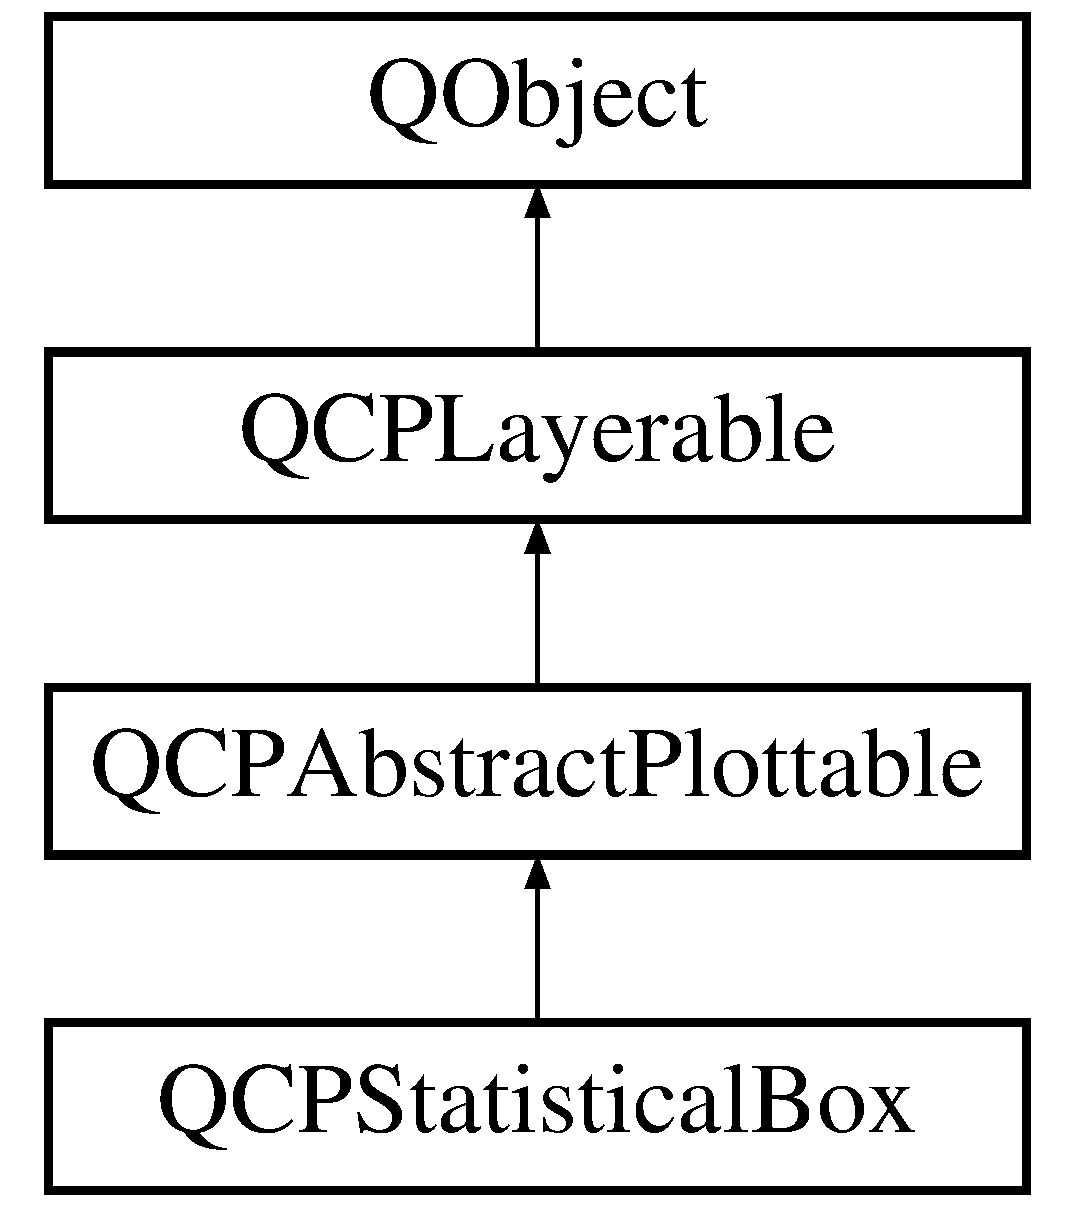
\includegraphics[height=4.000000cm]{class_q_c_p_statistical_box}
\end{center}
\end{figure}
\subsection*{Public Member Functions}
\begin{DoxyCompactItemize}
\item 
\hyperlink{class_q_c_p_statistical_box_a75c2b3e7fcd0741cc981693a2ba63b27}{Q\+C\+P\+Statistical\+Box} (\hyperlink{class_q_c_p_axis}{Q\+C\+P\+Axis} $\ast$key\+Axis, \hyperlink{class_q_c_p_axis}{Q\+C\+P\+Axis} $\ast$value\+Axis)
\item 
\hypertarget{class_q_c_p_statistical_box_a0543a2d25346376ba44a42817206cc42}{}\label{class_q_c_p_statistical_box_a0543a2d25346376ba44a42817206cc42} 
double {\bfseries key} () const
\item 
\hypertarget{class_q_c_p_statistical_box_ac5d07f908a9c49c81e2c7ff9dc8831e2}{}\label{class_q_c_p_statistical_box_ac5d07f908a9c49c81e2c7ff9dc8831e2} 
double {\bfseries minimum} () const
\item 
\hypertarget{class_q_c_p_statistical_box_afe9c3814cb02e3dffbe260f6bdb42d5e}{}\label{class_q_c_p_statistical_box_afe9c3814cb02e3dffbe260f6bdb42d5e} 
double {\bfseries lower\+Quartile} () const
\item 
\hypertarget{class_q_c_p_statistical_box_acde7599a12b0f73653ae8c681bf0bda0}{}\label{class_q_c_p_statistical_box_acde7599a12b0f73653ae8c681bf0bda0} 
double {\bfseries median} () const
\item 
\hypertarget{class_q_c_p_statistical_box_affa4149e6abe33edb734c611410939b6}{}\label{class_q_c_p_statistical_box_affa4149e6abe33edb734c611410939b6} 
double {\bfseries upper\+Quartile} () const
\item 
\hypertarget{class_q_c_p_statistical_box_a5ca15d360056689b6fe9180b835e26c9}{}\label{class_q_c_p_statistical_box_a5ca15d360056689b6fe9180b835e26c9} 
double {\bfseries maximum} () const
\item 
\hypertarget{class_q_c_p_statistical_box_a0a2c04824caeeabc4987a7a3ccf6b693}{}\label{class_q_c_p_statistical_box_a0a2c04824caeeabc4987a7a3ccf6b693} 
Q\+Vector$<$ double $>$ {\bfseries outliers} () const
\item 
\hypertarget{class_q_c_p_statistical_box_ae589b7481dec6ef8e50ebb6492d296f1}{}\label{class_q_c_p_statistical_box_ae589b7481dec6ef8e50ebb6492d296f1} 
double {\bfseries width} () const
\item 
\hypertarget{class_q_c_p_statistical_box_aacfa6686c7cf4af18794ec02354f4782}{}\label{class_q_c_p_statistical_box_aacfa6686c7cf4af18794ec02354f4782} 
double {\bfseries whisker\+Width} () const
\item 
\hypertarget{class_q_c_p_statistical_box_a67e5144f07645fe25c31001c460817fc}{}\label{class_q_c_p_statistical_box_a67e5144f07645fe25c31001c460817fc} 
Q\+Pen {\bfseries whisker\+Pen} () const
\item 
\hypertarget{class_q_c_p_statistical_box_a47ed9ad9d2ca65640319a2f071982ed4}{}\label{class_q_c_p_statistical_box_a47ed9ad9d2ca65640319a2f071982ed4} 
Q\+Pen {\bfseries whisker\+Bar\+Pen} () const
\item 
\hypertarget{class_q_c_p_statistical_box_af767bc7b6b477d005535314b35aca683}{}\label{class_q_c_p_statistical_box_af767bc7b6b477d005535314b35aca683} 
Q\+Pen {\bfseries median\+Pen} () const
\item 
\hypertarget{class_q_c_p_statistical_box_aef92e38fcb8e5041a44c2e01886e3b66}{}\label{class_q_c_p_statistical_box_aef92e38fcb8e5041a44c2e01886e3b66} 
\hyperlink{class_q_c_p_scatter_style}{Q\+C\+P\+Scatter\+Style} {\bfseries outlier\+Style} () const
\item 
void \hyperlink{class_q_c_p_statistical_box_a84a1c6d34b2f9af40bca0c527d51e97e}{set\+Key} (double key)
\item 
void \hyperlink{class_q_c_p_statistical_box_a84ff7cc61ba44890f0c3e0c99c19941e}{set\+Minimum} (double value)
\item 
void \hyperlink{class_q_c_p_statistical_box_a680941af5e23d902013962fa67223f9e}{set\+Lower\+Quartile} (double value)
\item 
void \hyperlink{class_q_c_p_statistical_box_a65970e77a897da4ecb4b15300868aad3}{set\+Median} (double value)
\item 
void \hyperlink{class_q_c_p_statistical_box_a65a1375f941c5a2077b5201229e89346}{set\+Upper\+Quartile} (double value)
\item 
void \hyperlink{class_q_c_p_statistical_box_acec5ad1901f00f2c5387cfb4d9787eb3}{set\+Maximum} (double value)
\item 
void \hyperlink{class_q_c_p_statistical_box_af9bc09620e0bf93bf444ee35e5800d1d}{set\+Outliers} (const Q\+Vector$<$ double $>$ \&values)
\item 
void \hyperlink{class_q_c_p_statistical_box_adf50c57b635edb12470c0e4a986aff37}{set\+Data} (double key, double minimum, double lower\+Quartile, double median, double upper\+Quartile, double maximum)
\item 
void \hyperlink{class_q_c_p_statistical_box_a0b62775bd67301b1eba5c785f2b26f14}{set\+Width} (double width)
\item 
void \hyperlink{class_q_c_p_statistical_box_adf378812446bd66f34d1f7f293d991cd}{set\+Whisker\+Width} (double width)
\item 
void \hyperlink{class_q_c_p_statistical_box_a4a5034cb3b9b040444df05ab1684620b}{set\+Whisker\+Pen} (const Q\+Pen \&pen)
\item 
void \hyperlink{class_q_c_p_statistical_box_aa8d3e503897788e1abf68dc74b5f147f}{set\+Whisker\+Bar\+Pen} (const Q\+Pen \&pen)
\item 
void \hyperlink{class_q_c_p_statistical_box_a7260ac55b669f5d0a74f16d5ca84c52c}{set\+Median\+Pen} (const Q\+Pen \&pen)
\item 
void \hyperlink{class_q_c_p_statistical_box_ad5241943422eb8e58360a97e99ad6aa7}{set\+Outlier\+Style} (const \hyperlink{class_q_c_p_scatter_style}{Q\+C\+P\+Scatter\+Style} \&style)
\item 
virtual void \hyperlink{class_q_c_p_statistical_box_a19112994449df0c20287858436cc68e3}{clear\+Data} ()
\item 
virtual double \hyperlink{class_q_c_p_statistical_box_a0153ac16326b94450afbca208e3f9961}{select\+Test} (const Q\+PointF \&pos, bool only\+Selectable, Q\+Variant $\ast$details=0) const
\end{DoxyCompactItemize}
\subsection*{Protected Member Functions}
\begin{DoxyCompactItemize}
\item 
\hypertarget{class_q_c_p_statistical_box_a753b62761217dd6b92f8a29e286a1317}{}\label{class_q_c_p_statistical_box_a753b62761217dd6b92f8a29e286a1317} 
virtual void {\bfseries draw} (\hyperlink{class_q_c_p_painter}{Q\+C\+P\+Painter} $\ast$painter)
\item 
\hypertarget{class_q_c_p_statistical_box_a41c6193fd24f5c1b6c754e7bcfe3e174}{}\label{class_q_c_p_statistical_box_a41c6193fd24f5c1b6c754e7bcfe3e174} 
virtual void {\bfseries draw\+Legend\+Icon} (\hyperlink{class_q_c_p_painter}{Q\+C\+P\+Painter} $\ast$painter, const Q\+RectF \&rect) const
\item 
\hypertarget{class_q_c_p_statistical_box_ac17d9d68e41be25b7f0e8a47f9a5d225}{}\label{class_q_c_p_statistical_box_ac17d9d68e41be25b7f0e8a47f9a5d225} 
virtual \hyperlink{class_q_c_p_range}{Q\+C\+P\+Range} {\bfseries get\+Key\+Range} (bool \&found\+Range, \hyperlink{class_q_c_p_abstract_plottable_a661743478a1d3c09d28ec2711d7653d8}{Sign\+Domain} in\+Sign\+Domain=\hyperlink{class_q_c_p_abstract_plottable_a661743478a1d3c09d28ec2711d7653d8a082b98cfb91a7363a3b5cd17b0c1cd60}{sd\+Both}) const
\item 
\hypertarget{class_q_c_p_statistical_box_a13958798713d4bb58b94e148b409877d}{}\label{class_q_c_p_statistical_box_a13958798713d4bb58b94e148b409877d} 
virtual \hyperlink{class_q_c_p_range}{Q\+C\+P\+Range} {\bfseries get\+Value\+Range} (bool \&found\+Range, \hyperlink{class_q_c_p_abstract_plottable_a661743478a1d3c09d28ec2711d7653d8}{Sign\+Domain} in\+Sign\+Domain=\hyperlink{class_q_c_p_abstract_plottable_a661743478a1d3c09d28ec2711d7653d8a082b98cfb91a7363a3b5cd17b0c1cd60}{sd\+Both}) const
\item 
\hypertarget{class_q_c_p_statistical_box_a699ede353d6a7207d9fb36dd3aabf348}{}\label{class_q_c_p_statistical_box_a699ede353d6a7207d9fb36dd3aabf348} 
virtual void {\bfseries draw\+Quartile\+Box} (\hyperlink{class_q_c_p_painter}{Q\+C\+P\+Painter} $\ast$painter, Q\+RectF $\ast$quartile\+Box=0) const
\item 
\hypertarget{class_q_c_p_statistical_box_a642b90dd4ab5ab6e16188a9230401bcc}{}\label{class_q_c_p_statistical_box_a642b90dd4ab5ab6e16188a9230401bcc} 
virtual void {\bfseries draw\+Median} (\hyperlink{class_q_c_p_painter}{Q\+C\+P\+Painter} $\ast$painter) const
\item 
\hypertarget{class_q_c_p_statistical_box_ae64401aa18b9c45d4d33f9b46cf4bbd0}{}\label{class_q_c_p_statistical_box_ae64401aa18b9c45d4d33f9b46cf4bbd0} 
virtual void {\bfseries draw\+Whiskers} (\hyperlink{class_q_c_p_painter}{Q\+C\+P\+Painter} $\ast$painter) const
\item 
\hypertarget{class_q_c_p_statistical_box_a8550e16af27b4e05d92bb337fb34324f}{}\label{class_q_c_p_statistical_box_a8550e16af27b4e05d92bb337fb34324f} 
virtual void {\bfseries draw\+Outliers} (\hyperlink{class_q_c_p_painter}{Q\+C\+P\+Painter} $\ast$painter) const
\end{DoxyCompactItemize}
\subsection*{Protected Attributes}
\begin{DoxyCompactItemize}
\item 
\hypertarget{class_q_c_p_statistical_box_a415e2f77a89396c2af999afe027bdf6c}{}\label{class_q_c_p_statistical_box_a415e2f77a89396c2af999afe027bdf6c} 
Q\+Vector$<$ double $>$ {\bfseries m\+Outliers}
\item 
\hypertarget{class_q_c_p_statistical_box_a86fd1d3be5c5bc11d11eda7517069af4}{}\label{class_q_c_p_statistical_box_a86fd1d3be5c5bc11d11eda7517069af4} 
double {\bfseries m\+Key}
\item 
\hypertarget{class_q_c_p_statistical_box_a7143ece4e7e5f9ac010739fbc390bf0c}{}\label{class_q_c_p_statistical_box_a7143ece4e7e5f9ac010739fbc390bf0c} 
double {\bfseries m\+Minimum}
\item 
\hypertarget{class_q_c_p_statistical_box_acac86cac93d9fa3d820b5aaa04ed96f6}{}\label{class_q_c_p_statistical_box_acac86cac93d9fa3d820b5aaa04ed96f6} 
double {\bfseries m\+Lower\+Quartile}
\item 
\hypertarget{class_q_c_p_statistical_box_ae43287ca13c8166bde2ac19bf0969d23}{}\label{class_q_c_p_statistical_box_ae43287ca13c8166bde2ac19bf0969d23} 
double {\bfseries m\+Median}
\item 
\hypertarget{class_q_c_p_statistical_box_a865afbcca332ee851aa45807381bc80e}{}\label{class_q_c_p_statistical_box_a865afbcca332ee851aa45807381bc80e} 
double {\bfseries m\+Upper\+Quartile}
\item 
\hypertarget{class_q_c_p_statistical_box_a16266f1e0e4e8e95b5d141c49479ef2e}{}\label{class_q_c_p_statistical_box_a16266f1e0e4e8e95b5d141c49479ef2e} 
double {\bfseries m\+Maximum}
\item 
\hypertarget{class_q_c_p_statistical_box_af365e40b0f706c3d76f857c7957f629d}{}\label{class_q_c_p_statistical_box_af365e40b0f706c3d76f857c7957f629d} 
double {\bfseries m\+Width}
\item 
\hypertarget{class_q_c_p_statistical_box_a4d166474f845d5db626e8b11a0815a6f}{}\label{class_q_c_p_statistical_box_a4d166474f845d5db626e8b11a0815a6f} 
double {\bfseries m\+Whisker\+Width}
\item 
\hypertarget{class_q_c_p_statistical_box_a25b7552499f0f090fcff02858b2265a5}{}\label{class_q_c_p_statistical_box_a25b7552499f0f090fcff02858b2265a5} 
Q\+Pen {\bfseries m\+Whisker\+Pen}
\item 
\hypertarget{class_q_c_p_statistical_box_aa719b1d722a9f82364df1497a6dc1da8}{}\label{class_q_c_p_statistical_box_aa719b1d722a9f82364df1497a6dc1da8} 
Q\+Pen {\bfseries m\+Whisker\+Bar\+Pen}
\item 
\hypertarget{class_q_c_p_statistical_box_a1af5b601049c575f778ae270f40c9443}{}\label{class_q_c_p_statistical_box_a1af5b601049c575f778ae270f40c9443} 
Q\+Pen {\bfseries m\+Median\+Pen}
\item 
\hypertarget{class_q_c_p_statistical_box_ae102e4187e1e6ba1f2df0f622b5171a4}{}\label{class_q_c_p_statistical_box_ae102e4187e1e6ba1f2df0f622b5171a4} 
\hyperlink{class_q_c_p_scatter_style}{Q\+C\+P\+Scatter\+Style} {\bfseries m\+Outlier\+Style}
\end{DoxyCompactItemize}
\subsection*{Friends}
\begin{DoxyCompactItemize}
\item 
\hypertarget{class_q_c_p_statistical_box_a1cdf9df76adcfae45261690aa0ca2198}{}\label{class_q_c_p_statistical_box_a1cdf9df76adcfae45261690aa0ca2198} 
class {\bfseries Q\+Custom\+Plot}
\item 
\hypertarget{class_q_c_p_statistical_box_a8429035e7adfbd7f05805a6530ad5e3b}{}\label{class_q_c_p_statistical_box_a8429035e7adfbd7f05805a6530ad5e3b} 
class {\bfseries Q\+C\+P\+Legend}
\end{DoxyCompactItemize}
\subsection*{Additional Inherited Members}


\subsection{Detailed Description}
A plottable representing a single statistical box in a plot. 



To plot data, assign it with the individual parameter functions or use \hyperlink{class_q_c_p_statistical_box_adf50c57b635edb12470c0e4a986aff37}{set\+Data} to set all parameters at once. The individual functions are\+: \begin{DoxyItemize}
\item \hyperlink{class_q_c_p_statistical_box_a84ff7cc61ba44890f0c3e0c99c19941e}{set\+Minimum} \item \hyperlink{class_q_c_p_statistical_box_a680941af5e23d902013962fa67223f9e}{set\+Lower\+Quartile} \item \hyperlink{class_q_c_p_statistical_box_a65970e77a897da4ecb4b15300868aad3}{set\+Median} \item \hyperlink{class_q_c_p_statistical_box_a65a1375f941c5a2077b5201229e89346}{set\+Upper\+Quartile} \item \hyperlink{class_q_c_p_statistical_box_acec5ad1901f00f2c5387cfb4d9787eb3}{set\+Maximum}\end{DoxyItemize}
Additionally you can define a list of outliers, drawn as scatter datapoints\+: \begin{DoxyItemize}
\item \hyperlink{class_q_c_p_statistical_box_af9bc09620e0bf93bf444ee35e5800d1d}{set\+Outliers}\end{DoxyItemize}
\hypertarget{class_q_c_p_statistical_box_appearance}{}\subsection{Changing the appearance}\label{class_q_c_p_statistical_box_appearance}
The appearance of the box itself is controlled via \hyperlink{class_q_c_p_abstract_plottable_ab74b09ae4c0e7e13142fe4b5bf46cac7}{set\+Pen} and \hyperlink{class_q_c_p_abstract_plottable_a7a4b92144dca6453a1f0f210e27edc74}{set\+Brush}. You may change the width of the box with \hyperlink{class_q_c_p_statistical_box_a0b62775bd67301b1eba5c785f2b26f14}{set\+Width} in plot coordinates (not pixels).

Analog functions exist for the minimum/maximum-\/whiskers\+: \hyperlink{class_q_c_p_statistical_box_a4a5034cb3b9b040444df05ab1684620b}{set\+Whisker\+Pen}, \hyperlink{class_q_c_p_statistical_box_aa8d3e503897788e1abf68dc74b5f147f}{set\+Whisker\+Bar\+Pen}, \hyperlink{class_q_c_p_statistical_box_adf378812446bd66f34d1f7f293d991cd}{set\+Whisker\+Width}. The whisker width is the width of the bar at the top (maximum) and bottom (minimum).

The median indicator line has its own pen, \hyperlink{class_q_c_p_statistical_box_a7260ac55b669f5d0a74f16d5ca84c52c}{set\+Median\+Pen}.

If the whisker backbone pen is changed, make sure to set the cap\+Style to Qt\+::\+Flat\+Cap. Else, the backbone line might exceed the whisker bars by a few pixels due to the pen cap being not perfectly flat.

The Outlier data points are drawn as normal scatter points. Their look can be controlled with \hyperlink{class_q_c_p_statistical_box_ad5241943422eb8e58360a97e99ad6aa7}{set\+Outlier\+Style}\hypertarget{class_q_c_p_statistical_box_usage}{}\subsection{Usage}\label{class_q_c_p_statistical_box_usage}
Like all data representing objects in \hyperlink{class_q_custom_plot}{Q\+Custom\+Plot}, the \hyperlink{class_q_c_p_statistical_box}{Q\+C\+P\+Statistical\+Box} is a plottable. Usually, you first create an instance and add it to the custom\+Plot\+: 
\begin{DoxyCodeInclude}
\end{DoxyCodeInclude}
and then modify the properties of the newly created plottable, e.\+g.\+: 
\begin{DoxyCodeInclude}
\end{DoxyCodeInclude}


\subsection{Constructor \& Destructor Documentation}
\hypertarget{class_q_c_p_statistical_box_a75c2b3e7fcd0741cc981693a2ba63b27}{}\label{class_q_c_p_statistical_box_a75c2b3e7fcd0741cc981693a2ba63b27} 
\index{Q\+C\+P\+Statistical\+Box@{Q\+C\+P\+Statistical\+Box}!Q\+C\+P\+Statistical\+Box@{Q\+C\+P\+Statistical\+Box}}
\index{Q\+C\+P\+Statistical\+Box@{Q\+C\+P\+Statistical\+Box}!Q\+C\+P\+Statistical\+Box@{Q\+C\+P\+Statistical\+Box}}
\subsubsection{\texorpdfstring{Q\+C\+P\+Statistical\+Box()}{QCPStatisticalBox()}}
{\footnotesize\ttfamily Q\+C\+P\+Statistical\+Box\+::\+Q\+C\+P\+Statistical\+Box (\begin{DoxyParamCaption}\item[{\hyperlink{class_q_c_p_axis}{Q\+C\+P\+Axis} $\ast$}]{key\+Axis,  }\item[{\hyperlink{class_q_c_p_axis}{Q\+C\+P\+Axis} $\ast$}]{value\+Axis }\end{DoxyParamCaption})\hspace{0.3cm}{\ttfamily [explicit]}}

Constructs a statistical box which uses {\itshape key\+Axis} as its key axis (\char`\"{}x\char`\"{}) and {\itshape value\+Axis} as its value axis (\char`\"{}y\char`\"{}). {\itshape key\+Axis} and {\itshape value\+Axis} must reside in the same \hyperlink{class_q_custom_plot}{Q\+Custom\+Plot} instance and not have the same orientation. If either of these restrictions is violated, a corresponding message is printed to the debug output (q\+Debug), the construction is not aborted, though.

The constructed statistical box can be added to the plot with \hyperlink{class_q_custom_plot_ab7ad9174f701f9c6f64e378df77927a6}{Q\+Custom\+Plot\+::add\+Plottable}, \hyperlink{class_q_custom_plot}{Q\+Custom\+Plot} then takes ownership of the statistical box. 

\subsection{Member Function Documentation}
\hypertarget{class_q_c_p_statistical_box_a19112994449df0c20287858436cc68e3}{}\label{class_q_c_p_statistical_box_a19112994449df0c20287858436cc68e3} 
\index{Q\+C\+P\+Statistical\+Box@{Q\+C\+P\+Statistical\+Box}!clear\+Data@{clear\+Data}}
\index{clear\+Data@{clear\+Data}!Q\+C\+P\+Statistical\+Box@{Q\+C\+P\+Statistical\+Box}}
\subsubsection{\texorpdfstring{clear\+Data()}{clearData()}}
{\footnotesize\ttfamily void Q\+C\+P\+Statistical\+Box\+::clear\+Data (\begin{DoxyParamCaption}{ }\end{DoxyParamCaption})\hspace{0.3cm}{\ttfamily [virtual]}}

Clears all data in the plottable. 

Implements \hyperlink{class_q_c_p_abstract_plottable_a86e5b8fd4b6ff4f4084e7ea4c573fc53}{Q\+C\+P\+Abstract\+Plottable}.

\hypertarget{class_q_c_p_statistical_box_a0153ac16326b94450afbca208e3f9961}{}\label{class_q_c_p_statistical_box_a0153ac16326b94450afbca208e3f9961} 
\index{Q\+C\+P\+Statistical\+Box@{Q\+C\+P\+Statistical\+Box}!select\+Test@{select\+Test}}
\index{select\+Test@{select\+Test}!Q\+C\+P\+Statistical\+Box@{Q\+C\+P\+Statistical\+Box}}
\subsubsection{\texorpdfstring{select\+Test()}{selectTest()}}
{\footnotesize\ttfamily double Q\+C\+P\+Statistical\+Box\+::select\+Test (\begin{DoxyParamCaption}\item[{const Q\+PointF \&}]{pos,  }\item[{bool}]{only\+Selectable,  }\item[{Q\+Variant $\ast$}]{details = {\ttfamily 0} }\end{DoxyParamCaption}) const\hspace{0.3cm}{\ttfamily [virtual]}}

This function is used to decide whether a click hits a layerable object or not.

{\itshape pos} is a point in pixel coordinates on the \hyperlink{class_q_custom_plot}{Q\+Custom\+Plot} surface. This function returns the shortest pixel distance of this point to the object. If the object is either invisible or the distance couldn\textquotesingle{}t be determined, -\/1.\+0 is returned. Further, if {\itshape only\+Selectable} is true and the object is not selectable, -\/1.\+0 is returned, too.

If the object is represented not by single lines but by an area like a \hyperlink{class_q_c_p_item_text}{Q\+C\+P\+Item\+Text} or the bars of a \hyperlink{class_q_c_p_bars}{Q\+C\+P\+Bars} plottable, a click inside the area should also be considered a hit. In these cases this function thus returns a constant value greater zero but still below the parent plot\textquotesingle{}s selection tolerance. (typically the selection\+Tolerance multiplied by 0.\+99).

Providing a constant value for area objects allows selecting line objects even when they are obscured by such area objects, by clicking close to the lines (i.\+e. closer than 0.\+99$\ast$selection\+Tolerance).

The actual setting of the selection state is not done by this function. This is handled by the parent \hyperlink{class_q_custom_plot}{Q\+Custom\+Plot} when the mouse\+Release\+Event occurs, and the finally selected object is notified via the select\+Event/deselect\+Event methods.

{\itshape details} is an optional output parameter. Every layerable subclass may place any information in {\itshape details}. This information will be passed to select\+Event when the parent \hyperlink{class_q_custom_plot}{Q\+Custom\+Plot} decides on the basis of this select\+Test call, that the object was successfully selected. The subsequent call to select\+Event will carry the {\itshape details}. This is useful for multi-\/part objects (like \hyperlink{class_q_c_p_axis}{Q\+C\+P\+Axis}). This way, a possibly complex calculation to decide which part was clicked is only done once in \hyperlink{class_q_c_p_statistical_box_a0153ac16326b94450afbca208e3f9961}{select\+Test}. The result (i.\+e. the actually clicked part) can then be placed in {\itshape details}. So in the subsequent select\+Event, the decision which part was selected doesn\textquotesingle{}t have to be done a second time for a single selection operation.

You may pass 0 as {\itshape details} to indicate that you are not interested in those selection details.

\begin{DoxySeeAlso}{See also}
select\+Event, deselect\+Event, \hyperlink{class_q_custom_plot_a5ee1e2f6ae27419deca53e75907c27e5}{Q\+Custom\+Plot\+::set\+Interactions} 
\end{DoxySeeAlso}


Implements \hyperlink{class_q_c_p_abstract_plottable_a38efe9641d972992a3d44204bc80ec1d}{Q\+C\+P\+Abstract\+Plottable}.

\hypertarget{class_q_c_p_statistical_box_adf50c57b635edb12470c0e4a986aff37}{}\label{class_q_c_p_statistical_box_adf50c57b635edb12470c0e4a986aff37} 
\index{Q\+C\+P\+Statistical\+Box@{Q\+C\+P\+Statistical\+Box}!set\+Data@{set\+Data}}
\index{set\+Data@{set\+Data}!Q\+C\+P\+Statistical\+Box@{Q\+C\+P\+Statistical\+Box}}
\subsubsection{\texorpdfstring{set\+Data()}{setData()}}
{\footnotesize\ttfamily void Q\+C\+P\+Statistical\+Box\+::set\+Data (\begin{DoxyParamCaption}\item[{double}]{key,  }\item[{double}]{minimum,  }\item[{double}]{lower\+Quartile,  }\item[{double}]{median,  }\item[{double}]{upper\+Quartile,  }\item[{double}]{maximum }\end{DoxyParamCaption})}

Sets all parameters of the statistical box plot at once.

\begin{DoxySeeAlso}{See also}
\hyperlink{class_q_c_p_statistical_box_a84a1c6d34b2f9af40bca0c527d51e97e}{set\+Key}, \hyperlink{class_q_c_p_statistical_box_a84ff7cc61ba44890f0c3e0c99c19941e}{set\+Minimum}, \hyperlink{class_q_c_p_statistical_box_a680941af5e23d902013962fa67223f9e}{set\+Lower\+Quartile}, \hyperlink{class_q_c_p_statistical_box_a65970e77a897da4ecb4b15300868aad3}{set\+Median}, \hyperlink{class_q_c_p_statistical_box_a65a1375f941c5a2077b5201229e89346}{set\+Upper\+Quartile}, \hyperlink{class_q_c_p_statistical_box_acec5ad1901f00f2c5387cfb4d9787eb3}{set\+Maximum} 
\end{DoxySeeAlso}
\hypertarget{class_q_c_p_statistical_box_a84a1c6d34b2f9af40bca0c527d51e97e}{}\label{class_q_c_p_statistical_box_a84a1c6d34b2f9af40bca0c527d51e97e} 
\index{Q\+C\+P\+Statistical\+Box@{Q\+C\+P\+Statistical\+Box}!set\+Key@{set\+Key}}
\index{set\+Key@{set\+Key}!Q\+C\+P\+Statistical\+Box@{Q\+C\+P\+Statistical\+Box}}
\subsubsection{\texorpdfstring{set\+Key()}{setKey()}}
{\footnotesize\ttfamily void Q\+C\+P\+Statistical\+Box\+::set\+Key (\begin{DoxyParamCaption}\item[{double}]{key }\end{DoxyParamCaption})}

Sets the key coordinate of the statistical box. \hypertarget{class_q_c_p_statistical_box_a680941af5e23d902013962fa67223f9e}{}\label{class_q_c_p_statistical_box_a680941af5e23d902013962fa67223f9e} 
\index{Q\+C\+P\+Statistical\+Box@{Q\+C\+P\+Statistical\+Box}!set\+Lower\+Quartile@{set\+Lower\+Quartile}}
\index{set\+Lower\+Quartile@{set\+Lower\+Quartile}!Q\+C\+P\+Statistical\+Box@{Q\+C\+P\+Statistical\+Box}}
\subsubsection{\texorpdfstring{set\+Lower\+Quartile()}{setLowerQuartile()}}
{\footnotesize\ttfamily void Q\+C\+P\+Statistical\+Box\+::set\+Lower\+Quartile (\begin{DoxyParamCaption}\item[{double}]{value }\end{DoxyParamCaption})}

Sets the parameter \char`\"{}lower Quartile\char`\"{} of the statistical box plot. This is the lower end of the box. The lower and the upper quartiles are the two statistical quartiles around the median of the sample, they contain 50\% of the sample data.

\begin{DoxySeeAlso}{See also}
\hyperlink{class_q_c_p_statistical_box_a65a1375f941c5a2077b5201229e89346}{set\+Upper\+Quartile}, \hyperlink{class_q_c_p_abstract_plottable_ab74b09ae4c0e7e13142fe4b5bf46cac7}{set\+Pen}, \hyperlink{class_q_c_p_abstract_plottable_a7a4b92144dca6453a1f0f210e27edc74}{set\+Brush}, \hyperlink{class_q_c_p_statistical_box_a0b62775bd67301b1eba5c785f2b26f14}{set\+Width} 
\end{DoxySeeAlso}
\hypertarget{class_q_c_p_statistical_box_acec5ad1901f00f2c5387cfb4d9787eb3}{}\label{class_q_c_p_statistical_box_acec5ad1901f00f2c5387cfb4d9787eb3} 
\index{Q\+C\+P\+Statistical\+Box@{Q\+C\+P\+Statistical\+Box}!set\+Maximum@{set\+Maximum}}
\index{set\+Maximum@{set\+Maximum}!Q\+C\+P\+Statistical\+Box@{Q\+C\+P\+Statistical\+Box}}
\subsubsection{\texorpdfstring{set\+Maximum()}{setMaximum()}}
{\footnotesize\ttfamily void Q\+C\+P\+Statistical\+Box\+::set\+Maximum (\begin{DoxyParamCaption}\item[{double}]{value }\end{DoxyParamCaption})}

Sets the parameter \char`\"{}maximum\char`\"{} of the statistical box plot. This is the position of the upper whisker, typically the maximum measurement of the sample that\textquotesingle{}s not considered an outlier.

\begin{DoxySeeAlso}{See also}
\hyperlink{class_q_c_p_statistical_box_a84ff7cc61ba44890f0c3e0c99c19941e}{set\+Minimum}, \hyperlink{class_q_c_p_statistical_box_a4a5034cb3b9b040444df05ab1684620b}{set\+Whisker\+Pen}, \hyperlink{class_q_c_p_statistical_box_aa8d3e503897788e1abf68dc74b5f147f}{set\+Whisker\+Bar\+Pen}, \hyperlink{class_q_c_p_statistical_box_adf378812446bd66f34d1f7f293d991cd}{set\+Whisker\+Width} 
\end{DoxySeeAlso}
\hypertarget{class_q_c_p_statistical_box_a65970e77a897da4ecb4b15300868aad3}{}\label{class_q_c_p_statistical_box_a65970e77a897da4ecb4b15300868aad3} 
\index{Q\+C\+P\+Statistical\+Box@{Q\+C\+P\+Statistical\+Box}!set\+Median@{set\+Median}}
\index{set\+Median@{set\+Median}!Q\+C\+P\+Statistical\+Box@{Q\+C\+P\+Statistical\+Box}}
\subsubsection{\texorpdfstring{set\+Median()}{setMedian()}}
{\footnotesize\ttfamily void Q\+C\+P\+Statistical\+Box\+::set\+Median (\begin{DoxyParamCaption}\item[{double}]{value }\end{DoxyParamCaption})}

Sets the parameter \char`\"{}median\char`\"{} of the statistical box plot. This is the value of the median mark inside the quartile box. The median separates the sample data in half (50\% of the sample data is below/above the median).

\begin{DoxySeeAlso}{See also}
\hyperlink{class_q_c_p_statistical_box_a7260ac55b669f5d0a74f16d5ca84c52c}{set\+Median\+Pen} 
\end{DoxySeeAlso}
\hypertarget{class_q_c_p_statistical_box_a7260ac55b669f5d0a74f16d5ca84c52c}{}\label{class_q_c_p_statistical_box_a7260ac55b669f5d0a74f16d5ca84c52c} 
\index{Q\+C\+P\+Statistical\+Box@{Q\+C\+P\+Statistical\+Box}!set\+Median\+Pen@{set\+Median\+Pen}}
\index{set\+Median\+Pen@{set\+Median\+Pen}!Q\+C\+P\+Statistical\+Box@{Q\+C\+P\+Statistical\+Box}}
\subsubsection{\texorpdfstring{set\+Median\+Pen()}{setMedianPen()}}
{\footnotesize\ttfamily void Q\+C\+P\+Statistical\+Box\+::set\+Median\+Pen (\begin{DoxyParamCaption}\item[{const Q\+Pen \&}]{pen }\end{DoxyParamCaption})}

Sets the pen used for drawing the median indicator line inside the statistical box. \hypertarget{class_q_c_p_statistical_box_a84ff7cc61ba44890f0c3e0c99c19941e}{}\label{class_q_c_p_statistical_box_a84ff7cc61ba44890f0c3e0c99c19941e} 
\index{Q\+C\+P\+Statistical\+Box@{Q\+C\+P\+Statistical\+Box}!set\+Minimum@{set\+Minimum}}
\index{set\+Minimum@{set\+Minimum}!Q\+C\+P\+Statistical\+Box@{Q\+C\+P\+Statistical\+Box}}
\subsubsection{\texorpdfstring{set\+Minimum()}{setMinimum()}}
{\footnotesize\ttfamily void Q\+C\+P\+Statistical\+Box\+::set\+Minimum (\begin{DoxyParamCaption}\item[{double}]{value }\end{DoxyParamCaption})}

Sets the parameter \char`\"{}minimum\char`\"{} of the statistical box plot. This is the position of the lower whisker, typically the minimum measurement of the sample that\textquotesingle{}s not considered an outlier.

\begin{DoxySeeAlso}{See also}
\hyperlink{class_q_c_p_statistical_box_acec5ad1901f00f2c5387cfb4d9787eb3}{set\+Maximum}, \hyperlink{class_q_c_p_statistical_box_a4a5034cb3b9b040444df05ab1684620b}{set\+Whisker\+Pen}, \hyperlink{class_q_c_p_statistical_box_aa8d3e503897788e1abf68dc74b5f147f}{set\+Whisker\+Bar\+Pen}, \hyperlink{class_q_c_p_statistical_box_adf378812446bd66f34d1f7f293d991cd}{set\+Whisker\+Width} 
\end{DoxySeeAlso}
\hypertarget{class_q_c_p_statistical_box_af9bc09620e0bf93bf444ee35e5800d1d}{}\label{class_q_c_p_statistical_box_af9bc09620e0bf93bf444ee35e5800d1d} 
\index{Q\+C\+P\+Statistical\+Box@{Q\+C\+P\+Statistical\+Box}!set\+Outliers@{set\+Outliers}}
\index{set\+Outliers@{set\+Outliers}!Q\+C\+P\+Statistical\+Box@{Q\+C\+P\+Statistical\+Box}}
\subsubsection{\texorpdfstring{set\+Outliers()}{setOutliers()}}
{\footnotesize\ttfamily void Q\+C\+P\+Statistical\+Box\+::set\+Outliers (\begin{DoxyParamCaption}\item[{const Q\+Vector$<$ double $>$ \&}]{values }\end{DoxyParamCaption})}

Sets a vector of outlier values that will be drawn as scatters. Any data points in the sample that are not within the whiskers (\hyperlink{class_q_c_p_statistical_box_a84ff7cc61ba44890f0c3e0c99c19941e}{set\+Minimum}, \hyperlink{class_q_c_p_statistical_box_acec5ad1901f00f2c5387cfb4d9787eb3}{set\+Maximum}) should be considered outliers and displayed as such.

\begin{DoxySeeAlso}{See also}
\hyperlink{class_q_c_p_statistical_box_ad5241943422eb8e58360a97e99ad6aa7}{set\+Outlier\+Style} 
\end{DoxySeeAlso}
\hypertarget{class_q_c_p_statistical_box_ad5241943422eb8e58360a97e99ad6aa7}{}\label{class_q_c_p_statistical_box_ad5241943422eb8e58360a97e99ad6aa7} 
\index{Q\+C\+P\+Statistical\+Box@{Q\+C\+P\+Statistical\+Box}!set\+Outlier\+Style@{set\+Outlier\+Style}}
\index{set\+Outlier\+Style@{set\+Outlier\+Style}!Q\+C\+P\+Statistical\+Box@{Q\+C\+P\+Statistical\+Box}}
\subsubsection{\texorpdfstring{set\+Outlier\+Style()}{setOutlierStyle()}}
{\footnotesize\ttfamily void Q\+C\+P\+Statistical\+Box\+::set\+Outlier\+Style (\begin{DoxyParamCaption}\item[{const \hyperlink{class_q_c_p_scatter_style}{Q\+C\+P\+Scatter\+Style} \&}]{style }\end{DoxyParamCaption})}

Sets the appearance of the outlier data points.

\begin{DoxySeeAlso}{See also}
\hyperlink{class_q_c_p_statistical_box_af9bc09620e0bf93bf444ee35e5800d1d}{set\+Outliers} 
\end{DoxySeeAlso}
\hypertarget{class_q_c_p_statistical_box_a65a1375f941c5a2077b5201229e89346}{}\label{class_q_c_p_statistical_box_a65a1375f941c5a2077b5201229e89346} 
\index{Q\+C\+P\+Statistical\+Box@{Q\+C\+P\+Statistical\+Box}!set\+Upper\+Quartile@{set\+Upper\+Quartile}}
\index{set\+Upper\+Quartile@{set\+Upper\+Quartile}!Q\+C\+P\+Statistical\+Box@{Q\+C\+P\+Statistical\+Box}}
\subsubsection{\texorpdfstring{set\+Upper\+Quartile()}{setUpperQuartile()}}
{\footnotesize\ttfamily void Q\+C\+P\+Statistical\+Box\+::set\+Upper\+Quartile (\begin{DoxyParamCaption}\item[{double}]{value }\end{DoxyParamCaption})}

Sets the parameter \char`\"{}upper Quartile\char`\"{} of the statistical box plot. This is the upper end of the box. The lower and the upper quartiles are the two statistical quartiles around the median of the sample, they contain 50\% of the sample data.

\begin{DoxySeeAlso}{See also}
\hyperlink{class_q_c_p_statistical_box_a680941af5e23d902013962fa67223f9e}{set\+Lower\+Quartile}, \hyperlink{class_q_c_p_abstract_plottable_ab74b09ae4c0e7e13142fe4b5bf46cac7}{set\+Pen}, \hyperlink{class_q_c_p_abstract_plottable_a7a4b92144dca6453a1f0f210e27edc74}{set\+Brush}, \hyperlink{class_q_c_p_statistical_box_a0b62775bd67301b1eba5c785f2b26f14}{set\+Width} 
\end{DoxySeeAlso}
\hypertarget{class_q_c_p_statistical_box_aa8d3e503897788e1abf68dc74b5f147f}{}\label{class_q_c_p_statistical_box_aa8d3e503897788e1abf68dc74b5f147f} 
\index{Q\+C\+P\+Statistical\+Box@{Q\+C\+P\+Statistical\+Box}!set\+Whisker\+Bar\+Pen@{set\+Whisker\+Bar\+Pen}}
\index{set\+Whisker\+Bar\+Pen@{set\+Whisker\+Bar\+Pen}!Q\+C\+P\+Statistical\+Box@{Q\+C\+P\+Statistical\+Box}}
\subsubsection{\texorpdfstring{set\+Whisker\+Bar\+Pen()}{setWhiskerBarPen()}}
{\footnotesize\ttfamily void Q\+C\+P\+Statistical\+Box\+::set\+Whisker\+Bar\+Pen (\begin{DoxyParamCaption}\item[{const Q\+Pen \&}]{pen }\end{DoxyParamCaption})}

Sets the pen used for drawing the whisker bars (Those are the lines parallel to the key axis at each end of the whisker backbone).

\begin{DoxySeeAlso}{See also}
\hyperlink{class_q_c_p_statistical_box_a4a5034cb3b9b040444df05ab1684620b}{set\+Whisker\+Pen} 
\end{DoxySeeAlso}
\hypertarget{class_q_c_p_statistical_box_a4a5034cb3b9b040444df05ab1684620b}{}\label{class_q_c_p_statistical_box_a4a5034cb3b9b040444df05ab1684620b} 
\index{Q\+C\+P\+Statistical\+Box@{Q\+C\+P\+Statistical\+Box}!set\+Whisker\+Pen@{set\+Whisker\+Pen}}
\index{set\+Whisker\+Pen@{set\+Whisker\+Pen}!Q\+C\+P\+Statistical\+Box@{Q\+C\+P\+Statistical\+Box}}
\subsubsection{\texorpdfstring{set\+Whisker\+Pen()}{setWhiskerPen()}}
{\footnotesize\ttfamily void Q\+C\+P\+Statistical\+Box\+::set\+Whisker\+Pen (\begin{DoxyParamCaption}\item[{const Q\+Pen \&}]{pen }\end{DoxyParamCaption})}

Sets the pen used for drawing the whisker backbone (That\textquotesingle{}s the line parallel to the value axis).

Make sure to set the {\itshape pen} cap\+Style to Qt\+::\+Flat\+Cap to prevent the whisker backbone from reaching a few pixels past the whisker bars, when using a non-\/zero pen width.

\begin{DoxySeeAlso}{See also}
\hyperlink{class_q_c_p_statistical_box_aa8d3e503897788e1abf68dc74b5f147f}{set\+Whisker\+Bar\+Pen} 
\end{DoxySeeAlso}
\hypertarget{class_q_c_p_statistical_box_adf378812446bd66f34d1f7f293d991cd}{}\label{class_q_c_p_statistical_box_adf378812446bd66f34d1f7f293d991cd} 
\index{Q\+C\+P\+Statistical\+Box@{Q\+C\+P\+Statistical\+Box}!set\+Whisker\+Width@{set\+Whisker\+Width}}
\index{set\+Whisker\+Width@{set\+Whisker\+Width}!Q\+C\+P\+Statistical\+Box@{Q\+C\+P\+Statistical\+Box}}
\subsubsection{\texorpdfstring{set\+Whisker\+Width()}{setWhiskerWidth()}}
{\footnotesize\ttfamily void Q\+C\+P\+Statistical\+Box\+::set\+Whisker\+Width (\begin{DoxyParamCaption}\item[{double}]{width }\end{DoxyParamCaption})}

Sets the width of the whiskers (\hyperlink{class_q_c_p_statistical_box_a84ff7cc61ba44890f0c3e0c99c19941e}{set\+Minimum}, \hyperlink{class_q_c_p_statistical_box_acec5ad1901f00f2c5387cfb4d9787eb3}{set\+Maximum}) in key coordinates.

\begin{DoxySeeAlso}{See also}
\hyperlink{class_q_c_p_statistical_box_a0b62775bd67301b1eba5c785f2b26f14}{set\+Width} 
\end{DoxySeeAlso}
\hypertarget{class_q_c_p_statistical_box_a0b62775bd67301b1eba5c785f2b26f14}{}\label{class_q_c_p_statistical_box_a0b62775bd67301b1eba5c785f2b26f14} 
\index{Q\+C\+P\+Statistical\+Box@{Q\+C\+P\+Statistical\+Box}!set\+Width@{set\+Width}}
\index{set\+Width@{set\+Width}!Q\+C\+P\+Statistical\+Box@{Q\+C\+P\+Statistical\+Box}}
\subsubsection{\texorpdfstring{set\+Width()}{setWidth()}}
{\footnotesize\ttfamily void Q\+C\+P\+Statistical\+Box\+::set\+Width (\begin{DoxyParamCaption}\item[{double}]{width }\end{DoxyParamCaption})}

Sets the width of the box in key coordinates.

\begin{DoxySeeAlso}{See also}
\hyperlink{class_q_c_p_statistical_box_adf378812446bd66f34d1f7f293d991cd}{set\+Whisker\+Width} 
\end{DoxySeeAlso}


The documentation for this class was generated from the following files\+:\begin{DoxyCompactItemize}
\item 
C\+:/\+Users/\+Jesse Jutson/\+Documents/\+Git\+Hub/\+F\+E\+S\+S\+G\+U\+I/\+F\+E\+S\+S-\/\+G\+U\+I/\hyperlink{qcustomplot_8h}{qcustomplot.\+h}\item 
C\+:/\+Users/\+Jesse Jutson/\+Documents/\+Git\+Hub/\+F\+E\+S\+S\+G\+U\+I/\+F\+E\+S\+S-\/\+G\+U\+I/\hyperlink{qcustomplot_8cpp}{qcustomplot.\+cpp}\end{DoxyCompactItemize}

\hypertarget{class_q_custom_plot}{}\section{Q\+Custom\+Plot Class Reference}
\label{class_q_custom_plot}\index{Q\+Custom\+Plot@{Q\+Custom\+Plot}}


The central class of the library. This is the Q\+Widget which displays the plot and interacts with the user.  


Inheritance diagram for Q\+Custom\+Plot\+:\begin{figure}[H]
\begin{center}
\leavevmode
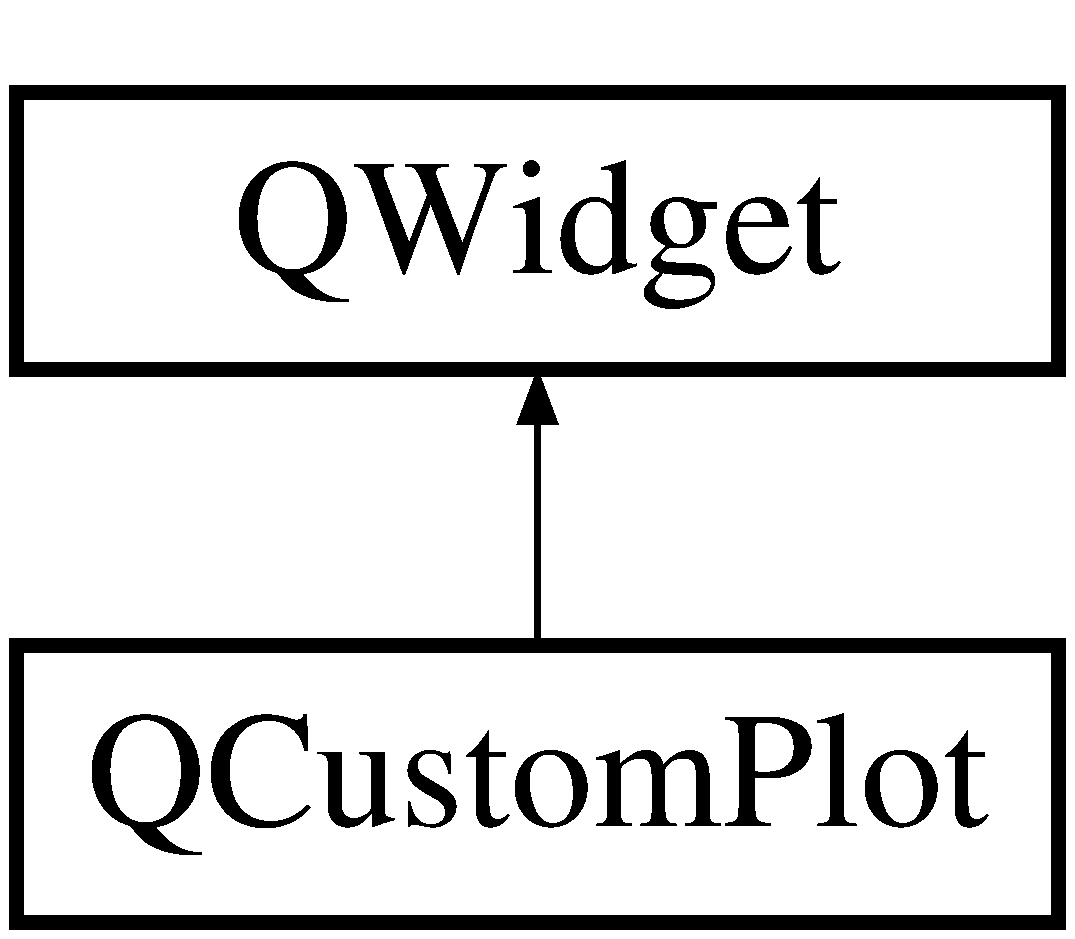
\includegraphics[height=2.000000cm]{class_q_custom_plot}
\end{center}
\end{figure}
\subsection*{Public Types}
\begin{DoxyCompactItemize}
\item 
enum \hyperlink{class_q_custom_plot_a75a8afbe6ef333b1f3d47abb25b9add7}{Layer\+Insert\+Mode} \{ \hyperlink{class_q_custom_plot_a75a8afbe6ef333b1f3d47abb25b9add7aee39cf650cd24e68552da0b697ce4a93}{lim\+Below}, 
\hyperlink{class_q_custom_plot_a75a8afbe6ef333b1f3d47abb25b9add7a062b0b7825650b432a713c0df6742d41}{lim\+Above}
 \}
\item 
enum \hyperlink{class_q_custom_plot_a45d61392d13042e712a956d27762aa39}{Refresh\+Priority} \{ \hyperlink{class_q_custom_plot_a45d61392d13042e712a956d27762aa39a0d4831572370d871f2b7cb88806bac59}{rp\+Immediate}, 
\hyperlink{class_q_custom_plot_a45d61392d13042e712a956d27762aa39aaaae083a19bc668597bf0f86e000f798}{rp\+Queued}, 
\hyperlink{class_q_custom_plot_a45d61392d13042e712a956d27762aa39adfa1f2387617168d9299f4c8ad15b332}{rp\+Hint}
 \}
\end{DoxyCompactItemize}
\subsection*{Signals}
\begin{DoxyCompactItemize}
\item 
void \hyperlink{class_q_custom_plot_a9b232142c64fcf273a953ee08e5b90e9}{mouse\+Double\+Click} (Q\+Mouse\+Event $\ast$event)
\item 
void \hyperlink{class_q_custom_plot_aca75bf9afb5dd19349c375de2a87a051}{mouse\+Press} (Q\+Mouse\+Event $\ast$event)
\item 
void \hyperlink{class_q_custom_plot_a742ca4f94688bed2a685fd8a56ce5704}{mouse\+Move} (Q\+Mouse\+Event $\ast$event)
\item 
void \hyperlink{class_q_custom_plot_ac8dc0ee6bb98e923c00b4ebafbe6134d}{mouse\+Release} (Q\+Mouse\+Event $\ast$event)
\item 
void \hyperlink{class_q_custom_plot_ac80a14206f99304a91d2aa55775ec3ff}{mouse\+Wheel} (Q\+Wheel\+Event $\ast$event)
\item 
void \hyperlink{class_q_custom_plot_a57e5efa8a854620e9bf62d31fc139f53}{plottable\+Click} (\hyperlink{class_q_c_p_abstract_plottable}{Q\+C\+P\+Abstract\+Plottable} $\ast$\hyperlink{class_q_custom_plot_a32de81ff53e263e785b83b52ecd99d6f}{plottable}, Q\+Mouse\+Event $\ast$event)
\item 
void \hyperlink{class_q_custom_plot_af2e6f1cea923dae437681d01ce7d0c31}{plottable\+Double\+Click} (\hyperlink{class_q_c_p_abstract_plottable}{Q\+C\+P\+Abstract\+Plottable} $\ast$\hyperlink{class_q_custom_plot_a32de81ff53e263e785b83b52ecd99d6f}{plottable}, Q\+Mouse\+Event $\ast$event)
\item 
void \hyperlink{class_q_custom_plot_ae16b51f52d2b7aebbc7e3e74e6ff2e4b}{item\+Click} (\hyperlink{class_q_c_p_abstract_item}{Q\+C\+P\+Abstract\+Item} $\ast$\hyperlink{class_q_custom_plot_ac042f2e78edd228ccf2f26b7fe215239}{item}, Q\+Mouse\+Event $\ast$event)
\item 
void \hyperlink{class_q_custom_plot_ac83aa9f5a3e9bb3efc9cdc763dcd42a6}{item\+Double\+Click} (\hyperlink{class_q_c_p_abstract_item}{Q\+C\+P\+Abstract\+Item} $\ast$\hyperlink{class_q_custom_plot_ac042f2e78edd228ccf2f26b7fe215239}{item}, Q\+Mouse\+Event $\ast$event)
\item 
void \hyperlink{class_q_custom_plot_abf635f8b56ab5c16d5de9f358543e82b}{axis\+Click} (\hyperlink{class_q_c_p_axis}{Q\+C\+P\+Axis} $\ast$axis, \hyperlink{class_q_c_p_axis_abee4c7a54c468b1385dfce2c898b115f}{Q\+C\+P\+Axis\+::\+Selectable\+Part} part, Q\+Mouse\+Event $\ast$event)
\item 
void \hyperlink{class_q_custom_plot_a6df35357460181a72da3e93d600f5256}{axis\+Double\+Click} (\hyperlink{class_q_c_p_axis}{Q\+C\+P\+Axis} $\ast$axis, \hyperlink{class_q_c_p_axis_abee4c7a54c468b1385dfce2c898b115f}{Q\+C\+P\+Axis\+::\+Selectable\+Part} part, Q\+Mouse\+Event $\ast$event)
\item 
void \hyperlink{class_q_custom_plot_a79cff0baafbca10a3aaf694d2d3b9ab3}{legend\+Click} (\hyperlink{class_q_c_p_legend}{Q\+C\+P\+Legend} $\ast$\hyperlink{class_q_custom_plot_a4eadcd237dc6a09938b68b16877fa6af}{legend}, \hyperlink{class_q_c_p_abstract_legend_item}{Q\+C\+P\+Abstract\+Legend\+Item} $\ast$\hyperlink{class_q_custom_plot_ac042f2e78edd228ccf2f26b7fe215239}{item}, Q\+Mouse\+Event $\ast$event)
\item 
void \hyperlink{class_q_custom_plot_a0250f835c044521df1619b132288bca7}{legend\+Double\+Click} (\hyperlink{class_q_c_p_legend}{Q\+C\+P\+Legend} $\ast$\hyperlink{class_q_custom_plot_a4eadcd237dc6a09938b68b16877fa6af}{legend}, \hyperlink{class_q_c_p_abstract_legend_item}{Q\+C\+P\+Abstract\+Legend\+Item} $\ast$\hyperlink{class_q_custom_plot_ac042f2e78edd228ccf2f26b7fe215239}{item}, Q\+Mouse\+Event $\ast$event)
\item 
void \hyperlink{class_q_custom_plot_a2137a819e518fee7edd1c0bf5984d8d6}{title\+Click} (Q\+Mouse\+Event $\ast$event, \hyperlink{class_q_c_p_plot_title}{Q\+C\+P\+Plot\+Title} $\ast$title)
\item 
void \hyperlink{class_q_custom_plot_ad51d65f6abf5edfaeef6e0519a4c1a2f}{title\+Double\+Click} (Q\+Mouse\+Event $\ast$event, \hyperlink{class_q_c_p_plot_title}{Q\+C\+P\+Plot\+Title} $\ast$title)
\item 
void \hyperlink{class_q_custom_plot_a500c64a109bc773c973ad274f2fa4190}{selection\+Changed\+By\+User} ()
\item 
void \hyperlink{class_q_custom_plot_a0cd30e29b73efd6afe096e44bc5956f5}{before\+Replot} ()
\item 
void \hyperlink{class_q_custom_plot_a6f4fa624af060bc5919c5f266cf426a0}{after\+Replot} ()
\end{DoxyCompactItemize}
\subsection*{Public Member Functions}
\begin{DoxyCompactItemize}
\item 
\hyperlink{class_q_custom_plot_a45b99626558651a6428b83972b0b34b8}{Q\+Custom\+Plot} (Q\+Widget $\ast$parent=0)
\item 
Q\+Rect \hyperlink{class_q_custom_plot_a19842409b18f556b256d05e97fffc670}{viewport} () const
\item 
\hypertarget{class_q_custom_plot_a5b9bbc838cb856e31b39c050fad49f9a}{}\label{class_q_custom_plot_a5b9bbc838cb856e31b39c050fad49f9a} 
Q\+Pixmap {\bfseries background} () const
\item 
\hypertarget{class_q_custom_plot_aac96f3a0f5070228ed13602976886b80}{}\label{class_q_custom_plot_aac96f3a0f5070228ed13602976886b80} 
bool {\bfseries background\+Scaled} () const
\item 
\hypertarget{class_q_custom_plot_af8f1ebfdbf48d7c49f95136475d55b14}{}\label{class_q_custom_plot_af8f1ebfdbf48d7c49f95136475d55b14} 
Qt\+::\+Aspect\+Ratio\+Mode {\bfseries background\+Scaled\+Mode} () const
\item 
\hyperlink{class_q_c_p_layout_grid}{Q\+C\+P\+Layout\+Grid} $\ast$ \hyperlink{class_q_custom_plot_af1a1f1f571237deb7c2bd34a5e9f018f}{plot\+Layout} () const
\item 
\hypertarget{class_q_custom_plot_a631762eb183aceecee73d30e108641ee}{}\label{class_q_custom_plot_a631762eb183aceecee73d30e108641ee} 
Q\+C\+P\+::\+Antialiased\+Elements {\bfseries antialiased\+Elements} () const
\item 
\hypertarget{class_q_custom_plot_a75571bc5b2167e83def132fc993091b3}{}\label{class_q_custom_plot_a75571bc5b2167e83def132fc993091b3} 
Q\+C\+P\+::\+Antialiased\+Elements {\bfseries not\+Antialiased\+Elements} () const
\item 
\hypertarget{class_q_custom_plot_ac4b87de13eaceadc8db5a66654197689}{}\label{class_q_custom_plot_ac4b87de13eaceadc8db5a66654197689} 
bool {\bfseries auto\+Add\+Plottable\+To\+Legend} () const
\item 
\hypertarget{class_q_custom_plot_a2c78c5fd2943c148ab76652801d3f2dc}{}\label{class_q_custom_plot_a2c78c5fd2943c148ab76652801d3f2dc} 
const Q\+C\+P\+::\+Interactions {\bfseries interactions} () const
\item 
\hypertarget{class_q_custom_plot_a5441d11013afeaf4b8f2ea06e8624a25}{}\label{class_q_custom_plot_a5441d11013afeaf4b8f2ea06e8624a25} 
int {\bfseries selection\+Tolerance} () const
\item 
\hypertarget{class_q_custom_plot_aca3f01f903fb250a3dd27104d92830be}{}\label{class_q_custom_plot_aca3f01f903fb250a3dd27104d92830be} 
bool {\bfseries no\+Antialiasing\+On\+Drag} () const
\item 
\hypertarget{class_q_custom_plot_ac724f4075822f74f7b676a790095b877}{}\label{class_q_custom_plot_ac724f4075822f74f7b676a790095b877} 
Q\+C\+P\+::\+Plotting\+Hints {\bfseries plotting\+Hints} () const
\item 
\hypertarget{class_q_custom_plot_a28182402ed11609c9a429f0788162d18}{}\label{class_q_custom_plot_a28182402ed11609c9a429f0788162d18} 
Qt\+::\+Keyboard\+Modifier {\bfseries multi\+Select\+Modifier} () const
\item 
void \hyperlink{class_q_custom_plot_a3f9bc4b939dd8aaba9339fd09f273fc4}{set\+Viewport} (const Q\+Rect \&rect)
\item 
void \hyperlink{class_q_custom_plot_a130358592cfca353ff3cf5571b49fb00}{set\+Background} (const Q\+Pixmap \&pm)
\item 
void \hyperlink{class_q_custom_plot_a8513971d6aa24d8b0d6a68d45b542130}{set\+Background} (const Q\+Pixmap \&pm, bool scaled, Qt\+::\+Aspect\+Ratio\+Mode mode=Qt\+::\+Keep\+Aspect\+Ratio\+By\+Expanding)
\item 
void \hyperlink{class_q_custom_plot_a8ed256cf467bfa7ba1f9feaae62c3bd0}{set\+Background} (const Q\+Brush \&brush)
\item 
void \hyperlink{class_q_custom_plot_a36f0fa1317325dc7b7efea615ee2de1f}{set\+Background\+Scaled} (bool scaled)
\item 
void \hyperlink{class_q_custom_plot_a4c0eb4865b7949f62e1cb97db04a3de0}{set\+Background\+Scaled\+Mode} (Qt\+::\+Aspect\+Ratio\+Mode mode)
\item 
void \hyperlink{class_q_custom_plot_af6f91e5eab1be85f67c556e98c3745e8}{set\+Antialiased\+Elements} (const Q\+C\+P\+::\+Antialiased\+Elements \&antialiased\+Elements)
\item 
void \hyperlink{class_q_custom_plot_aeef813bcf7efab8e765f9f87ec454691}{set\+Antialiased\+Element} (\hyperlink{namespace_q_c_p_ae55dbe315d41fe80f29ba88100843a0c}{Q\+C\+P\+::\+Antialiased\+Element} antialiased\+Element, bool enabled=true)
\item 
void \hyperlink{class_q_custom_plot_ae10d685b5eabea2999fb8775ca173c24}{set\+Not\+Antialiased\+Elements} (const Q\+C\+P\+::\+Antialiased\+Elements \&not\+Antialiased\+Elements)
\item 
void \hyperlink{class_q_custom_plot_afc657938a707c890e449ae89203a076d}{set\+Not\+Antialiased\+Element} (\hyperlink{namespace_q_c_p_ae55dbe315d41fe80f29ba88100843a0c}{Q\+C\+P\+::\+Antialiased\+Element} not\+Antialiased\+Element, bool enabled=true)
\item 
void \hyperlink{class_q_custom_plot_ad8858410c2db47b7104040a3aa61c3fc}{set\+Auto\+Add\+Plottable\+To\+Legend} (bool on)
\item 
void \hyperlink{class_q_custom_plot_a5ee1e2f6ae27419deca53e75907c27e5}{set\+Interactions} (const Q\+C\+P\+::\+Interactions \&interactions)
\item 
void \hyperlink{class_q_custom_plot_a422bf1bc6d56dac75a3d805d9a65902c}{set\+Interaction} (const \hyperlink{namespace_q_c_p_a2ad6bb6281c7c2d593d4277b44c2b037}{Q\+C\+P\+::\+Interaction} \&interaction, bool enabled=true)
\item 
void \hyperlink{class_q_custom_plot_a4dc31241d7b09680950e19e5f971ed93}{set\+Selection\+Tolerance} (int pixels)
\item 
void \hyperlink{class_q_custom_plot_a775bdcb6329d44701aeaa6135b0e5265}{set\+No\+Antialiasing\+On\+Drag} (bool enabled)
\item 
void \hyperlink{class_q_custom_plot_a94a33cbdadbbac5934843508bcfc210d}{set\+Plotting\+Hints} (const Q\+C\+P\+::\+Plotting\+Hints \&hints)
\item 
void \hyperlink{class_q_custom_plot_a3b7c97bb6c16464e9e15190c07abe9a9}{set\+Plotting\+Hint} (\hyperlink{namespace_q_c_p_a5400e5fcb9528d92002ddb938c1f4ef4}{Q\+C\+P\+::\+Plotting\+Hint} hint, bool enabled=true)
\item 
void \hyperlink{class_q_custom_plot_a8fc96e3b5138a06759a2a90c166df516}{set\+Multi\+Select\+Modifier} (Qt\+::\+Keyboard\+Modifier modifier)
\item 
\hyperlink{class_q_c_p_abstract_plottable}{Q\+C\+P\+Abstract\+Plottable} $\ast$ \hyperlink{class_q_custom_plot_a32de81ff53e263e785b83b52ecd99d6f}{plottable} (int index)
\item 
\hyperlink{class_q_c_p_abstract_plottable}{Q\+C\+P\+Abstract\+Plottable} $\ast$ \hyperlink{class_q_custom_plot_adea38bdc660da9412ba69fb939031567}{plottable} ()
\item 
bool \hyperlink{class_q_custom_plot_ab7ad9174f701f9c6f64e378df77927a6}{add\+Plottable} (\hyperlink{class_q_c_p_abstract_plottable}{Q\+C\+P\+Abstract\+Plottable} $\ast$\hyperlink{class_q_custom_plot_a32de81ff53e263e785b83b52ecd99d6f}{plottable})
\item 
bool \hyperlink{class_q_custom_plot_af3dafd56884208474f311d6226513ab2}{remove\+Plottable} (\hyperlink{class_q_c_p_abstract_plottable}{Q\+C\+P\+Abstract\+Plottable} $\ast$\hyperlink{class_q_custom_plot_a32de81ff53e263e785b83b52ecd99d6f}{plottable})
\item 
bool \hyperlink{class_q_custom_plot_afc210e0021480f8119bccf37839dbcc8}{remove\+Plottable} (int index)
\item 
int \hyperlink{class_q_custom_plot_a9a409bb3201878adb7ffba1c89c4e004}{clear\+Plottables} ()
\item 
int \hyperlink{class_q_custom_plot_a5f4f15991c14bf9ad659bb2a19dfbed4}{plottable\+Count} () const
\item 
Q\+List$<$ \hyperlink{class_q_c_p_abstract_plottable}{Q\+C\+P\+Abstract\+Plottable} $\ast$ $>$ \hyperlink{class_q_custom_plot_a747faaab57c56891e901a1e97fa4359a}{selected\+Plottables} () const
\item 
\hyperlink{class_q_c_p_abstract_plottable}{Q\+C\+P\+Abstract\+Plottable} $\ast$ \hyperlink{class_q_custom_plot_acddbbd8b16dd633f0d94e5a736fbd8cf}{plottable\+At} (const Q\+PointF \&pos, bool only\+Selectable=false) const
\item 
bool \hyperlink{class_q_custom_plot_a72cefbfbb9e699940e37be605bd9c51e}{has\+Plottable} (\hyperlink{class_q_c_p_abstract_plottable}{Q\+C\+P\+Abstract\+Plottable} $\ast$\hyperlink{class_q_custom_plot_a32de81ff53e263e785b83b52ecd99d6f}{plottable}) const
\item 
\hyperlink{class_q_c_p_graph}{Q\+C\+P\+Graph} $\ast$ \hyperlink{class_q_custom_plot_a6ecae130f684b25276fb47bd3a5875c6}{graph} (int index) const
\item 
\hyperlink{class_q_c_p_graph}{Q\+C\+P\+Graph} $\ast$ \hyperlink{class_q_custom_plot_aac190865a67f19af3fdf2136774997af}{graph} () const
\item 
\hyperlink{class_q_c_p_graph}{Q\+C\+P\+Graph} $\ast$ \hyperlink{class_q_custom_plot_a6fb2873d35a8a8089842d81a70a54167}{add\+Graph} (\hyperlink{class_q_c_p_axis}{Q\+C\+P\+Axis} $\ast$key\+Axis=0, \hyperlink{class_q_c_p_axis}{Q\+C\+P\+Axis} $\ast$value\+Axis=0)
\item 
bool \hyperlink{class_q_custom_plot_a903561be895fb6528a770d66ac5e6713}{remove\+Graph} (\hyperlink{class_q_c_p_graph}{Q\+C\+P\+Graph} $\ast$\hyperlink{class_q_custom_plot_a6ecae130f684b25276fb47bd3a5875c6}{graph})
\item 
bool \hyperlink{class_q_custom_plot_a9554b3d2d5b10c0f884bd4010b6c192c}{remove\+Graph} (int index)
\item 
int \hyperlink{class_q_custom_plot_ab0f3abff2d2f7df3668b5836f39207fa}{clear\+Graphs} ()
\item 
int \hyperlink{class_q_custom_plot_a5e1787cdde868c4d3790f9ebc8207d90}{graph\+Count} () const
\item 
Q\+List$<$ \hyperlink{class_q_c_p_graph}{Q\+C\+P\+Graph} $\ast$ $>$ \hyperlink{class_q_custom_plot_ad3547aded026d8a9ae6ef13a69080d06}{selected\+Graphs} () const
\item 
\hyperlink{class_q_c_p_abstract_item}{Q\+C\+P\+Abstract\+Item} $\ast$ \hyperlink{class_q_custom_plot_ac042f2e78edd228ccf2f26b7fe215239}{item} (int index) const
\item 
\hyperlink{class_q_c_p_abstract_item}{Q\+C\+P\+Abstract\+Item} $\ast$ \hyperlink{class_q_custom_plot_a12eb2a283cf10a8a9176c01c0443e83e}{item} () const
\item 
bool \hyperlink{class_q_custom_plot_aa500620379262321685cb7a7674cbd2a}{add\+Item} (\hyperlink{class_q_c_p_abstract_item}{Q\+C\+P\+Abstract\+Item} $\ast$\hyperlink{class_q_custom_plot_ac042f2e78edd228ccf2f26b7fe215239}{item})
\item 
bool \hyperlink{class_q_custom_plot_ae04446557292551e8fb6e2c106e1848d}{remove\+Item} (\hyperlink{class_q_c_p_abstract_item}{Q\+C\+P\+Abstract\+Item} $\ast$\hyperlink{class_q_custom_plot_ac042f2e78edd228ccf2f26b7fe215239}{item})
\item 
bool \hyperlink{class_q_custom_plot_abcfdda3d601c0441cab136137d715dea}{remove\+Item} (int index)
\item 
int \hyperlink{class_q_custom_plot_abdfd07d4f0591d0cf967f85013fd3645}{clear\+Items} ()
\item 
int \hyperlink{class_q_custom_plot_a16025daf0341f9362be3080e404424c2}{item\+Count} () const
\item 
Q\+List$<$ \hyperlink{class_q_c_p_abstract_item}{Q\+C\+P\+Abstract\+Item} $\ast$ $>$ \hyperlink{class_q_custom_plot_afda487bcf2d6cf1a57173d82495e29ba}{selected\+Items} () const
\item 
\hyperlink{class_q_c_p_abstract_item}{Q\+C\+P\+Abstract\+Item} $\ast$ \hyperlink{class_q_custom_plot_ac08578e0e6c059c83a8d340ba0038e8e}{item\+At} (const Q\+PointF \&pos, bool only\+Selectable=false) const
\item 
bool \hyperlink{class_q_custom_plot_af0b57f35646079f93fa6161a65b36109}{has\+Item} (\hyperlink{class_q_c_p_abstract_item}{Q\+C\+P\+Abstract\+Item} $\ast$\hyperlink{class_q_custom_plot_ac042f2e78edd228ccf2f26b7fe215239}{item}) const
\item 
\hyperlink{class_q_c_p_layer}{Q\+C\+P\+Layer} $\ast$ \hyperlink{class_q_custom_plot_a0a96244e7773b242ef23c32b7bdfb159}{layer} (const Q\+String \&name) const
\item 
\hyperlink{class_q_c_p_layer}{Q\+C\+P\+Layer} $\ast$ \hyperlink{class_q_custom_plot_acbb570f4c24306e7c2324d40bfe157c2}{layer} (int index) const
\item 
\hyperlink{class_q_c_p_layer}{Q\+C\+P\+Layer} $\ast$ \hyperlink{class_q_custom_plot_a0421d647f420b0b4c57aec1708857af5}{current\+Layer} () const
\item 
bool \hyperlink{class_q_custom_plot_a73a6dc47c653bb6f8f030abca5a11852}{set\+Current\+Layer} (const Q\+String \&name)
\item 
bool \hyperlink{class_q_custom_plot_a23a4d3cadad1a0063c5fe19aac5659e6}{set\+Current\+Layer} (\hyperlink{class_q_c_p_layer}{Q\+C\+P\+Layer} $\ast$\hyperlink{class_q_custom_plot_a0a96244e7773b242ef23c32b7bdfb159}{layer})
\item 
int \hyperlink{class_q_custom_plot_afa45d61e65292026f4c58c9c88c2cef0}{layer\+Count} () const
\item 
bool \hyperlink{class_q_custom_plot_ad5255393df078448bb6ac83fa5db5f52}{add\+Layer} (const Q\+String \&name, \hyperlink{class_q_c_p_layer}{Q\+C\+P\+Layer} $\ast$other\+Layer=0, \hyperlink{class_q_custom_plot_a75a8afbe6ef333b1f3d47abb25b9add7}{Layer\+Insert\+Mode} insert\+Mode=\hyperlink{class_q_custom_plot_a75a8afbe6ef333b1f3d47abb25b9add7a062b0b7825650b432a713c0df6742d41}{lim\+Above})
\item 
bool \hyperlink{class_q_custom_plot_a40f75e342c5eaab6a86066a42a0e2a94}{remove\+Layer} (\hyperlink{class_q_c_p_layer}{Q\+C\+P\+Layer} $\ast$\hyperlink{class_q_custom_plot_a0a96244e7773b242ef23c32b7bdfb159}{layer})
\item 
bool \hyperlink{class_q_custom_plot_ae896140beff19424e9e9e02d6e331104}{move\+Layer} (\hyperlink{class_q_c_p_layer}{Q\+C\+P\+Layer} $\ast$\hyperlink{class_q_custom_plot_a0a96244e7773b242ef23c32b7bdfb159}{layer}, \hyperlink{class_q_c_p_layer}{Q\+C\+P\+Layer} $\ast$other\+Layer, \hyperlink{class_q_custom_plot_a75a8afbe6ef333b1f3d47abb25b9add7}{Layer\+Insert\+Mode} insert\+Mode=\hyperlink{class_q_custom_plot_a75a8afbe6ef333b1f3d47abb25b9add7a062b0b7825650b432a713c0df6742d41}{lim\+Above})
\item 
int \hyperlink{class_q_custom_plot_a8f85940aaac50efb466287d9d2d04ec6}{axis\+Rect\+Count} () const
\item 
\hyperlink{class_q_c_p_axis_rect}{Q\+C\+P\+Axis\+Rect} $\ast$ \hyperlink{class_q_custom_plot_ae5eefcb5f6ca26689b1fd4f6e25b42f9}{axis\+Rect} (int index=0) const
\item 
Q\+List$<$ \hyperlink{class_q_c_p_axis_rect}{Q\+C\+P\+Axis\+Rect} $\ast$ $>$ \hyperlink{class_q_custom_plot_a12af771429e2d7e313c8c5d5fca068fe}{axis\+Rects} () const
\item 
\hyperlink{class_q_c_p_layout_element}{Q\+C\+P\+Layout\+Element} $\ast$ \hyperlink{class_q_custom_plot_afaa1d304e0287d140fd238e90889ef3c}{layout\+Element\+At} (const Q\+PointF \&pos) const
\item 
Q\+\_\+\+S\+L\+OT void \hyperlink{class_q_custom_plot_ad86528f2cee6c7e446dea4a6e8839935}{rescale\+Axes} (bool only\+Visible\+Plottables=false)
\item 
Q\+List$<$ \hyperlink{class_q_c_p_axis}{Q\+C\+P\+Axis} $\ast$ $>$ \hyperlink{class_q_custom_plot_a7e6b07792b1cb2c31681596582d14dbe}{selected\+Axes} () const
\item 
Q\+List$<$ \hyperlink{class_q_c_p_legend}{Q\+C\+P\+Legend} $\ast$ $>$ \hyperlink{class_q_custom_plot_ac87624ddff1cbf4064781a8e8ae321c4}{selected\+Legends} () const
\item 
Q\+\_\+\+S\+L\+OT void \hyperlink{class_q_custom_plot_a9d4808ab925b003054085246c92a257c}{deselect\+All} ()
\item 
bool \hyperlink{class_q_custom_plot_a632da44c6d94ea8b271eb483b08b5114}{save\+Pdf} (const Q\+String \&file\+Name, bool no\+Cosmetic\+Pen=false, int width=0, int height=0, const Q\+String \&pdf\+Creator=Q\+String(), const Q\+String \&pdf\+Title=Q\+String())
\item 
bool \hyperlink{class_q_custom_plot_a7636261aff1f6d25c9da749ece3fc8b8}{save\+Png} (const Q\+String \&file\+Name, int width=0, int height=0, double scale=1.\+0, int quality=-\/1)
\item 
bool \hyperlink{class_q_custom_plot_a490c722092d1771e8ce4a7a73dfd84ab}{save\+Jpg} (const Q\+String \&file\+Name, int width=0, int height=0, double scale=1.\+0, int quality=-\/1)
\item 
bool \hyperlink{class_q_custom_plot_a6629d9e8e6da4bf18055ee0257fdce9a}{save\+Bmp} (const Q\+String \&file\+Name, int width=0, int height=0, double scale=1.\+0)
\item 
bool \hyperlink{class_q_custom_plot_ab528b84cf92baabe29b1d0ef2f77c93e}{save\+Rastered} (const Q\+String \&file\+Name, int width, int height, double scale, const char $\ast$format, int quality=-\/1)
\item 
Q\+Pixmap \hyperlink{class_q_custom_plot_aabb974d71ce96c137dc04eb6eab844fe}{to\+Pixmap} (int width=0, int height=0, double scale=1.\+0)
\item 
void \hyperlink{class_q_custom_plot_a1be68d5c0f1e086d6374d1340a193fb9}{to\+Painter} (\hyperlink{class_q_c_p_painter}{Q\+C\+P\+Painter} $\ast$painter, int width=0, int height=0)
\item 
Q\+\_\+\+S\+L\+OT void \hyperlink{class_q_custom_plot_a606fd384b2a637ce2c24899bcbde77d6}{replot} (\hyperlink{class_q_custom_plot_a45d61392d13042e712a956d27762aa39}{Q\+Custom\+Plot\+::\+Refresh\+Priority} refresh\+Priority=\hyperlink{class_q_custom_plot_a45d61392d13042e712a956d27762aa39adfa1f2387617168d9299f4c8ad15b332}{Q\+Custom\+Plot\+::rp\+Hint})
\end{DoxyCompactItemize}
\subsection*{Public Attributes}
\begin{DoxyCompactItemize}
\item 
\hyperlink{class_q_c_p_axis}{Q\+C\+P\+Axis} $\ast$ \hyperlink{class_q_custom_plot_a9a79cd0158a4c7f30cbc702f0fd800e4}{x\+Axis}
\item 
\hyperlink{class_q_c_p_axis}{Q\+C\+P\+Axis} $\ast$ \hyperlink{class_q_custom_plot_af6fea5679725b152c14facd920b19367}{y\+Axis}
\item 
\hyperlink{class_q_c_p_axis}{Q\+C\+P\+Axis} $\ast$ \hyperlink{class_q_custom_plot_ada41599f22cad901c030f3dcbdd82fd9}{x\+Axis2}
\item 
\hyperlink{class_q_c_p_axis}{Q\+C\+P\+Axis} $\ast$ \hyperlink{class_q_custom_plot_af13fdc5bce7d0fabd640f13ba805c0b7}{y\+Axis2}
\item 
\hyperlink{class_q_c_p_legend}{Q\+C\+P\+Legend} $\ast$ \hyperlink{class_q_custom_plot_a4eadcd237dc6a09938b68b16877fa6af}{legend}
\end{DoxyCompactItemize}
\subsection*{Protected Member Functions}
\begin{DoxyCompactItemize}
\item 
\hypertarget{class_q_custom_plot_a0f7d90553493be687da80544f7244ad2}{}\label{class_q_custom_plot_a0f7d90553493be687da80544f7244ad2} 
virtual Q\+Size {\bfseries minimum\+Size\+Hint} () const
\item 
\hypertarget{class_q_custom_plot_a51601831bc7d5403d5e729347a10ba33}{}\label{class_q_custom_plot_a51601831bc7d5403d5e729347a10ba33} 
virtual Q\+Size {\bfseries size\+Hint} () const
\item 
\hypertarget{class_q_custom_plot_a2bbc3b1c24bfcc8a7cc1f3008cdd9b73}{}\label{class_q_custom_plot_a2bbc3b1c24bfcc8a7cc1f3008cdd9b73} 
virtual void {\bfseries paint\+Event} (Q\+Paint\+Event $\ast$event)
\item 
\hypertarget{class_q_custom_plot_a13e05523a40c3f08875df5cde85cf0d9}{}\label{class_q_custom_plot_a13e05523a40c3f08875df5cde85cf0d9} 
virtual void {\bfseries resize\+Event} (Q\+Resize\+Event $\ast$event)
\item 
\hypertarget{class_q_custom_plot_a77591913a5b543bdc465dd5e08325a49}{}\label{class_q_custom_plot_a77591913a5b543bdc465dd5e08325a49} 
virtual void {\bfseries mouse\+Double\+Click\+Event} (Q\+Mouse\+Event $\ast$event)
\item 
\hypertarget{class_q_custom_plot_abce84fa2c71e47b9295d67e8fce84bb4}{}\label{class_q_custom_plot_abce84fa2c71e47b9295d67e8fce84bb4} 
virtual void {\bfseries mouse\+Press\+Event} (Q\+Mouse\+Event $\ast$event)
\item 
\hypertarget{class_q_custom_plot_ac64727a4f442770f6e5e6be2d0530843}{}\label{class_q_custom_plot_ac64727a4f442770f6e5e6be2d0530843} 
virtual void {\bfseries mouse\+Move\+Event} (Q\+Mouse\+Event $\ast$event)
\item 
\hypertarget{class_q_custom_plot_a724e97d2e8c03e68adac5f4b6164a1b3}{}\label{class_q_custom_plot_a724e97d2e8c03e68adac5f4b6164a1b3} 
virtual void {\bfseries mouse\+Release\+Event} (Q\+Mouse\+Event $\ast$event)
\item 
\hypertarget{class_q_custom_plot_a7b8bd7e8d3a1d23a8595e9c6a6b76ef1}{}\label{class_q_custom_plot_a7b8bd7e8d3a1d23a8595e9c6a6b76ef1} 
virtual void {\bfseries wheel\+Event} (Q\+Wheel\+Event $\ast$event)
\item 
\hypertarget{class_q_custom_plot_ad7a7d878bf050f101a43008e7d8fdb52}{}\label{class_q_custom_plot_ad7a7d878bf050f101a43008e7d8fdb52} 
virtual void {\bfseries draw} (\hyperlink{class_q_c_p_painter}{Q\+C\+P\+Painter} $\ast$painter)
\item 
\hypertarget{class_q_custom_plot_a8b46607021c463c94709d3504951cb47}{}\label{class_q_custom_plot_a8b46607021c463c94709d3504951cb47} 
virtual void {\bfseries axis\+Removed} (\hyperlink{class_q_c_p_axis}{Q\+C\+P\+Axis} $\ast$axis)
\item 
\hypertarget{class_q_custom_plot_a9d173454555021c9ffd4f675c4d9037a}{}\label{class_q_custom_plot_a9d173454555021c9ffd4f675c4d9037a} 
virtual void {\bfseries legend\+Removed} (\hyperlink{class_q_c_p_legend}{Q\+C\+P\+Legend} $\ast$\hyperlink{class_q_custom_plot_a4eadcd237dc6a09938b68b16877fa6af}{legend})
\item 
\hypertarget{class_q_custom_plot_a7f1ca67a66d37b6d260a0b93de08f3bd}{}\label{class_q_custom_plot_a7f1ca67a66d37b6d260a0b93de08f3bd} 
void {\bfseries update\+Layer\+Indices} () const
\item 
\hypertarget{class_q_custom_plot_a12536fa6d5deb34ec620acb5134ca82a}{}\label{class_q_custom_plot_a12536fa6d5deb34ec620acb5134ca82a} 
\hyperlink{class_q_c_p_layerable}{Q\+C\+P\+Layerable} $\ast$ {\bfseries layerable\+At} (const Q\+PointF \&pos, bool only\+Selectable, Q\+Variant $\ast$selection\+Details=0) const
\item 
\hypertarget{class_q_custom_plot_a05dd52438cee4353b18c1e53a439008d}{}\label{class_q_custom_plot_a05dd52438cee4353b18c1e53a439008d} 
void {\bfseries draw\+Background} (\hyperlink{class_q_c_p_painter}{Q\+C\+P\+Painter} $\ast$painter)
\end{DoxyCompactItemize}
\subsection*{Protected Attributes}
\begin{DoxyCompactItemize}
\item 
\hypertarget{class_q_custom_plot_ac0a7c38a715526c257cff95774f83ab6}{}\label{class_q_custom_plot_ac0a7c38a715526c257cff95774f83ab6} 
Q\+Rect {\bfseries m\+Viewport}
\item 
\hypertarget{class_q_custom_plot_ac97298756882a0eecd98151679850ac1}{}\label{class_q_custom_plot_ac97298756882a0eecd98151679850ac1} 
\hyperlink{class_q_c_p_layout_grid}{Q\+C\+P\+Layout\+Grid} $\ast$ {\bfseries m\+Plot\+Layout}
\item 
\hypertarget{class_q_custom_plot_aaf3ea6a4cb04d35a149cc9a0cdac3394}{}\label{class_q_custom_plot_aaf3ea6a4cb04d35a149cc9a0cdac3394} 
bool {\bfseries m\+Auto\+Add\+Plottable\+To\+Legend}
\item 
\hypertarget{class_q_custom_plot_a62bf8e4e7f8d23fc1e9301ba0148269f}{}\label{class_q_custom_plot_a62bf8e4e7f8d23fc1e9301ba0148269f} 
Q\+List$<$ \hyperlink{class_q_c_p_abstract_plottable}{Q\+C\+P\+Abstract\+Plottable} $\ast$ $>$ {\bfseries m\+Plottables}
\item 
\hypertarget{class_q_custom_plot_adaf8d407d72a725169d7dbed2ee386bb}{}\label{class_q_custom_plot_adaf8d407d72a725169d7dbed2ee386bb} 
Q\+List$<$ \hyperlink{class_q_c_p_graph}{Q\+C\+P\+Graph} $\ast$ $>$ {\bfseries m\+Graphs}
\item 
\hypertarget{class_q_custom_plot_a6a93905372326e31e98d6c3bc8953ec8}{}\label{class_q_custom_plot_a6a93905372326e31e98d6c3bc8953ec8} 
Q\+List$<$ \hyperlink{class_q_c_p_abstract_item}{Q\+C\+P\+Abstract\+Item} $\ast$ $>$ {\bfseries m\+Items}
\item 
\hypertarget{class_q_custom_plot_a72ee313041b873d76c198793ce7e6c37}{}\label{class_q_custom_plot_a72ee313041b873d76c198793ce7e6c37} 
Q\+List$<$ \hyperlink{class_q_c_p_layer}{Q\+C\+P\+Layer} $\ast$ $>$ {\bfseries m\+Layers}
\item 
\hypertarget{class_q_custom_plot_aa333200629256830e273873b582a5524}{}\label{class_q_custom_plot_aa333200629256830e273873b582a5524} 
Q\+C\+P\+::\+Antialiased\+Elements {\bfseries m\+Antialiased\+Elements}
\item 
\hypertarget{class_q_custom_plot_a2b6ebcad00a90ba07f146cefcd4293da}{}\label{class_q_custom_plot_a2b6ebcad00a90ba07f146cefcd4293da} 
Q\+C\+P\+::\+Antialiased\+Elements {\bfseries m\+Not\+Antialiased\+Elements}
\item 
\hypertarget{class_q_custom_plot_ad717377ceba7493b4b32f0bcbbdf1895}{}\label{class_q_custom_plot_ad717377ceba7493b4b32f0bcbbdf1895} 
Q\+C\+P\+::\+Interactions {\bfseries m\+Interactions}
\item 
\hypertarget{class_q_custom_plot_abc36e12dd0482117ad810a800c847722}{}\label{class_q_custom_plot_abc36e12dd0482117ad810a800c847722} 
int {\bfseries m\+Selection\+Tolerance}
\item 
\hypertarget{class_q_custom_plot_ac83df968435f6b8ec79f2993ab9124e8}{}\label{class_q_custom_plot_ac83df968435f6b8ec79f2993ab9124e8} 
bool {\bfseries m\+No\+Antialiasing\+On\+Drag}
\item 
\hypertarget{class_q_custom_plot_a3aef5de4ac012178e3293248e9c63737}{}\label{class_q_custom_plot_a3aef5de4ac012178e3293248e9c63737} 
Q\+Brush {\bfseries m\+Background\+Brush}
\item 
\hypertarget{class_q_custom_plot_ae8f4677399324a78c5f8dbfb95a34f90}{}\label{class_q_custom_plot_ae8f4677399324a78c5f8dbfb95a34f90} 
Q\+Pixmap {\bfseries m\+Background\+Pixmap}
\item 
\hypertarget{class_q_custom_plot_a081bf046501d52642dc6d7e3bdb97d57}{}\label{class_q_custom_plot_a081bf046501d52642dc6d7e3bdb97d57} 
Q\+Pixmap {\bfseries m\+Scaled\+Background\+Pixmap}
\item 
\hypertarget{class_q_custom_plot_a62fe584b20680b1b2e1c7efb5c5416a5}{}\label{class_q_custom_plot_a62fe584b20680b1b2e1c7efb5c5416a5} 
bool {\bfseries m\+Background\+Scaled}
\item 
\hypertarget{class_q_custom_plot_ab82e8a5e3ad6b486f95d6da8bf49e9aa}{}\label{class_q_custom_plot_ab82e8a5e3ad6b486f95d6da8bf49e9aa} 
Qt\+::\+Aspect\+Ratio\+Mode {\bfseries m\+Background\+Scaled\+Mode}
\item 
\hypertarget{class_q_custom_plot_aa27569c92e74395af10151357d268628}{}\label{class_q_custom_plot_aa27569c92e74395af10151357d268628} 
\hyperlink{class_q_c_p_layer}{Q\+C\+P\+Layer} $\ast$ {\bfseries m\+Current\+Layer}
\item 
\hypertarget{class_q_custom_plot_aa184197a6101a9cc5807469e1d006c9e}{}\label{class_q_custom_plot_aa184197a6101a9cc5807469e1d006c9e} 
Q\+C\+P\+::\+Plotting\+Hints {\bfseries m\+Plotting\+Hints}
\item 
\hypertarget{class_q_custom_plot_a0e97e701c5671e7e463d2ce0211d0f8a}{}\label{class_q_custom_plot_a0e97e701c5671e7e463d2ce0211d0f8a} 
Qt\+::\+Keyboard\+Modifier {\bfseries m\+Multi\+Select\+Modifier}
\item 
\hypertarget{class_q_custom_plot_a753630df96e0672098d9e88bd41d1913}{}\label{class_q_custom_plot_a753630df96e0672098d9e88bd41d1913} 
Q\+Pixmap {\bfseries m\+Paint\+Buffer}
\item 
\hypertarget{class_q_custom_plot_ac57090da95056ae4dd67be67adfa85bd}{}\label{class_q_custom_plot_ac57090da95056ae4dd67be67adfa85bd} 
Q\+Point {\bfseries m\+Mouse\+Press\+Pos}
\item 
\hypertarget{class_q_custom_plot_a2f2e8b25e59cf3cf7b15e4767c02e747}{}\label{class_q_custom_plot_a2f2e8b25e59cf3cf7b15e4767c02e747} 
Q\+Pointer$<$ \hyperlink{class_q_c_p_layout_element}{Q\+C\+P\+Layout\+Element} $>$ {\bfseries m\+Mouse\+Event\+Element}
\item 
\hypertarget{class_q_custom_plot_ab30daeca6612c3948afd368dce5f1c39}{}\label{class_q_custom_plot_ab30daeca6612c3948afd368dce5f1c39} 
bool {\bfseries m\+Replotting}
\end{DoxyCompactItemize}
\subsection*{Friends}
\begin{DoxyCompactItemize}
\item 
\hypertarget{class_q_custom_plot_a8429035e7adfbd7f05805a6530ad5e3b}{}\label{class_q_custom_plot_a8429035e7adfbd7f05805a6530ad5e3b} 
class {\bfseries Q\+C\+P\+Legend}
\item 
\hypertarget{class_q_custom_plot_af123edeca169ec7a31958a1d714e1a8a}{}\label{class_q_custom_plot_af123edeca169ec7a31958a1d714e1a8a} 
class {\bfseries Q\+C\+P\+Axis}
\item 
\hypertarget{class_q_custom_plot_a5dbf96bf7664c1b6fce49063eeea6eef}{}\label{class_q_custom_plot_a5dbf96bf7664c1b6fce49063eeea6eef} 
class {\bfseries Q\+C\+P\+Layer}
\item 
\hypertarget{class_q_custom_plot_acbf20ecb140f66c5fd1bc64ae0762990}{}\label{class_q_custom_plot_acbf20ecb140f66c5fd1bc64ae0762990} 
class {\bfseries Q\+C\+P\+Axis\+Rect}
\end{DoxyCompactItemize}


\subsection{Detailed Description}
The central class of the library. This is the Q\+Widget which displays the plot and interacts with the user. 

For tutorials on how to use \hyperlink{class_q_custom_plot}{Q\+Custom\+Plot}, see the website~\newline
\href{http://www.qcustomplot.com/}{\tt http\+://www.\+qcustomplot.\+com/} 

\subsection{Member Enumeration Documentation}
\hypertarget{class_q_custom_plot_a75a8afbe6ef333b1f3d47abb25b9add7}{}\label{class_q_custom_plot_a75a8afbe6ef333b1f3d47abb25b9add7} 
\index{Q\+Custom\+Plot@{Q\+Custom\+Plot}!Layer\+Insert\+Mode@{Layer\+Insert\+Mode}}
\index{Layer\+Insert\+Mode@{Layer\+Insert\+Mode}!Q\+Custom\+Plot@{Q\+Custom\+Plot}}
\subsubsection{\texorpdfstring{Layer\+Insert\+Mode}{LayerInsertMode}}
{\footnotesize\ttfamily enum \hyperlink{class_q_custom_plot_a75a8afbe6ef333b1f3d47abb25b9add7}{Q\+Custom\+Plot\+::\+Layer\+Insert\+Mode}}

Defines how a layer should be inserted relative to an other layer.

\begin{DoxySeeAlso}{See also}
\hyperlink{class_q_custom_plot_ad5255393df078448bb6ac83fa5db5f52}{add\+Layer}, \hyperlink{class_q_custom_plot_ae896140beff19424e9e9e02d6e331104}{move\+Layer} 
\end{DoxySeeAlso}
\begin{DoxyEnumFields}{Enumerator}
\raisebox{\heightof{T}}[0pt][0pt]{\index{lim\+Below@{lim\+Below}!Q\+Custom\+Plot@{Q\+Custom\+Plot}}\index{Q\+Custom\+Plot@{Q\+Custom\+Plot}!lim\+Below@{lim\+Below}}}\hypertarget{class_q_custom_plot_a75a8afbe6ef333b1f3d47abb25b9add7aee39cf650cd24e68552da0b697ce4a93}{}\label{class_q_custom_plot_a75a8afbe6ef333b1f3d47abb25b9add7aee39cf650cd24e68552da0b697ce4a93} 
lim\+Below&Layer is inserted below other layer. \\
\hline

\raisebox{\heightof{T}}[0pt][0pt]{\index{lim\+Above@{lim\+Above}!Q\+Custom\+Plot@{Q\+Custom\+Plot}}\index{Q\+Custom\+Plot@{Q\+Custom\+Plot}!lim\+Above@{lim\+Above}}}\hypertarget{class_q_custom_plot_a75a8afbe6ef333b1f3d47abb25b9add7a062b0b7825650b432a713c0df6742d41}{}\label{class_q_custom_plot_a75a8afbe6ef333b1f3d47abb25b9add7a062b0b7825650b432a713c0df6742d41} 
lim\+Above&Layer is inserted above other layer. \\
\hline

\end{DoxyEnumFields}
\hypertarget{class_q_custom_plot_a45d61392d13042e712a956d27762aa39}{}\label{class_q_custom_plot_a45d61392d13042e712a956d27762aa39} 
\index{Q\+Custom\+Plot@{Q\+Custom\+Plot}!Refresh\+Priority@{Refresh\+Priority}}
\index{Refresh\+Priority@{Refresh\+Priority}!Q\+Custom\+Plot@{Q\+Custom\+Plot}}
\subsubsection{\texorpdfstring{Refresh\+Priority}{RefreshPriority}}
{\footnotesize\ttfamily enum \hyperlink{class_q_custom_plot_a45d61392d13042e712a956d27762aa39}{Q\+Custom\+Plot\+::\+Refresh\+Priority}}

Defines with what timing the \hyperlink{class_q_custom_plot}{Q\+Custom\+Plot} surface is refreshed after a replot.

\begin{DoxySeeAlso}{See also}
\hyperlink{class_q_custom_plot_a606fd384b2a637ce2c24899bcbde77d6}{replot} 
\end{DoxySeeAlso}
\begin{DoxyEnumFields}{Enumerator}
\raisebox{\heightof{T}}[0pt][0pt]{\index{rp\+Immediate@{rp\+Immediate}!Q\+Custom\+Plot@{Q\+Custom\+Plot}}\index{Q\+Custom\+Plot@{Q\+Custom\+Plot}!rp\+Immediate@{rp\+Immediate}}}\hypertarget{class_q_custom_plot_a45d61392d13042e712a956d27762aa39a0d4831572370d871f2b7cb88806bac59}{}\label{class_q_custom_plot_a45d61392d13042e712a956d27762aa39a0d4831572370d871f2b7cb88806bac59} 
rp\+Immediate&The \hyperlink{class_q_custom_plot}{Q\+Custom\+Plot} surface is immediately refreshed, by calling Q\+Widget\+::repaint() after the replot. \\
\hline

\raisebox{\heightof{T}}[0pt][0pt]{\index{rp\+Queued@{rp\+Queued}!Q\+Custom\+Plot@{Q\+Custom\+Plot}}\index{Q\+Custom\+Plot@{Q\+Custom\+Plot}!rp\+Queued@{rp\+Queued}}}\hypertarget{class_q_custom_plot_a45d61392d13042e712a956d27762aa39aaaae083a19bc668597bf0f86e000f798}{}\label{class_q_custom_plot_a45d61392d13042e712a956d27762aa39aaaae083a19bc668597bf0f86e000f798} 
rp\+Queued&Queues the refresh such that it is performed at a slightly delayed point in time after the replot, by calling Q\+Widget\+::update() after the replot. \\
\hline

\raisebox{\heightof{T}}[0pt][0pt]{\index{rp\+Hint@{rp\+Hint}!Q\+Custom\+Plot@{Q\+Custom\+Plot}}\index{Q\+Custom\+Plot@{Q\+Custom\+Plot}!rp\+Hint@{rp\+Hint}}}\hypertarget{class_q_custom_plot_a45d61392d13042e712a956d27762aa39adfa1f2387617168d9299f4c8ad15b332}{}\label{class_q_custom_plot_a45d61392d13042e712a956d27762aa39adfa1f2387617168d9299f4c8ad15b332} 
rp\+Hint&Whether to use immediate repaint or queued update depends on whether the plotting hint \hyperlink{namespace_q_c_p_a5400e5fcb9528d92002ddb938c1f4ef4aa3090dafa0e0f9a28c579c79d6c2d283}{Q\+C\+P\+::ph\+Force\+Repaint} is set, see \hyperlink{class_q_custom_plot_a94a33cbdadbbac5934843508bcfc210d}{set\+Plotting\+Hints}. \\
\hline

\end{DoxyEnumFields}


\subsection{Constructor \& Destructor Documentation}
\hypertarget{class_q_custom_plot_a45b99626558651a6428b83972b0b34b8}{}\label{class_q_custom_plot_a45b99626558651a6428b83972b0b34b8} 
\index{Q\+Custom\+Plot@{Q\+Custom\+Plot}!Q\+Custom\+Plot@{Q\+Custom\+Plot}}
\index{Q\+Custom\+Plot@{Q\+Custom\+Plot}!Q\+Custom\+Plot@{Q\+Custom\+Plot}}
\subsubsection{\texorpdfstring{Q\+Custom\+Plot()}{QCustomPlot()}}
{\footnotesize\ttfamily Q\+Custom\+Plot\+::\+Q\+Custom\+Plot (\begin{DoxyParamCaption}\item[{Q\+Widget $\ast$}]{parent = {\ttfamily 0} }\end{DoxyParamCaption})\hspace{0.3cm}{\ttfamily [explicit]}}

Constructs a \hyperlink{class_q_custom_plot}{Q\+Custom\+Plot} and sets reasonable default values. 

\subsection{Member Function Documentation}
\hypertarget{class_q_custom_plot_a6fb2873d35a8a8089842d81a70a54167}{}\label{class_q_custom_plot_a6fb2873d35a8a8089842d81a70a54167} 
\index{Q\+Custom\+Plot@{Q\+Custom\+Plot}!add\+Graph@{add\+Graph}}
\index{add\+Graph@{add\+Graph}!Q\+Custom\+Plot@{Q\+Custom\+Plot}}
\subsubsection{\texorpdfstring{add\+Graph()}{addGraph()}}
{\footnotesize\ttfamily \hyperlink{class_q_c_p_graph}{Q\+C\+P\+Graph} $\ast$ Q\+Custom\+Plot\+::add\+Graph (\begin{DoxyParamCaption}\item[{\hyperlink{class_q_c_p_axis}{Q\+C\+P\+Axis} $\ast$}]{key\+Axis = {\ttfamily 0},  }\item[{\hyperlink{class_q_c_p_axis}{Q\+C\+P\+Axis} $\ast$}]{value\+Axis = {\ttfamily 0} }\end{DoxyParamCaption})}

Creates a new graph inside the plot. If {\itshape key\+Axis} and {\itshape value\+Axis} are left unspecified (0), the bottom (x\+Axis) is used as key and the left (y\+Axis) is used as value axis. If specified, {\itshape key\+Axis} and {\itshape value\+Axis} must reside in this \hyperlink{class_q_custom_plot}{Q\+Custom\+Plot}.

{\itshape key\+Axis} will be used as key axis (typically \char`\"{}x\char`\"{}) and {\itshape value\+Axis} as value axis (typically \char`\"{}y\char`\"{}) for the graph.

Returns a pointer to the newly created graph, or 0 if adding the graph failed.

\begin{DoxySeeAlso}{See also}
\hyperlink{class_q_custom_plot_a6ecae130f684b25276fb47bd3a5875c6}{graph}, \hyperlink{class_q_custom_plot_a5e1787cdde868c4d3790f9ebc8207d90}{graph\+Count}, \hyperlink{class_q_custom_plot_a903561be895fb6528a770d66ac5e6713}{remove\+Graph}, \hyperlink{class_q_custom_plot_ab0f3abff2d2f7df3668b5836f39207fa}{clear\+Graphs} 
\end{DoxySeeAlso}
\hypertarget{class_q_custom_plot_aa500620379262321685cb7a7674cbd2a}{}\label{class_q_custom_plot_aa500620379262321685cb7a7674cbd2a} 
\index{Q\+Custom\+Plot@{Q\+Custom\+Plot}!add\+Item@{add\+Item}}
\index{add\+Item@{add\+Item}!Q\+Custom\+Plot@{Q\+Custom\+Plot}}
\subsubsection{\texorpdfstring{add\+Item()}{addItem()}}
{\footnotesize\ttfamily bool Q\+Custom\+Plot\+::add\+Item (\begin{DoxyParamCaption}\item[{\hyperlink{class_q_c_p_abstract_item}{Q\+C\+P\+Abstract\+Item} $\ast$}]{item }\end{DoxyParamCaption})}

Adds the specified item to the plot. \hyperlink{class_q_custom_plot}{Q\+Custom\+Plot} takes ownership of the item.

Returns true on success, i.\+e. when {\itshape item} wasn\textquotesingle{}t already in the plot and the parent plot of {\itshape item} is this \hyperlink{class_q_custom_plot}{Q\+Custom\+Plot}.

\begin{DoxySeeAlso}{See also}
\hyperlink{class_q_custom_plot_ac042f2e78edd228ccf2f26b7fe215239}{item}, \hyperlink{class_q_custom_plot_a16025daf0341f9362be3080e404424c2}{item\+Count}, \hyperlink{class_q_custom_plot_ae04446557292551e8fb6e2c106e1848d}{remove\+Item}, \hyperlink{class_q_custom_plot_abdfd07d4f0591d0cf967f85013fd3645}{clear\+Items} 
\end{DoxySeeAlso}
\hypertarget{class_q_custom_plot_ad5255393df078448bb6ac83fa5db5f52}{}\label{class_q_custom_plot_ad5255393df078448bb6ac83fa5db5f52} 
\index{Q\+Custom\+Plot@{Q\+Custom\+Plot}!add\+Layer@{add\+Layer}}
\index{add\+Layer@{add\+Layer}!Q\+Custom\+Plot@{Q\+Custom\+Plot}}
\subsubsection{\texorpdfstring{add\+Layer()}{addLayer()}}
{\footnotesize\ttfamily bool Q\+Custom\+Plot\+::add\+Layer (\begin{DoxyParamCaption}\item[{const Q\+String \&}]{name,  }\item[{\hyperlink{class_q_c_p_layer}{Q\+C\+P\+Layer} $\ast$}]{other\+Layer = {\ttfamily 0},  }\item[{\hyperlink{class_q_custom_plot_a75a8afbe6ef333b1f3d47abb25b9add7}{Q\+Custom\+Plot\+::\+Layer\+Insert\+Mode}}]{insert\+Mode = {\ttfamily \hyperlink{class_q_custom_plot_a75a8afbe6ef333b1f3d47abb25b9add7a062b0b7825650b432a713c0df6742d41}{lim\+Above}} }\end{DoxyParamCaption})}

Adds a new layer to this \hyperlink{class_q_custom_plot}{Q\+Custom\+Plot} instance. The new layer will have the name {\itshape name}, which must be unique. Depending on {\itshape insert\+Mode}, it is positioned either below or above {\itshape other\+Layer}.

Returns true on success, i.\+e. if there is no other layer named {\itshape name} and {\itshape other\+Layer} is a valid layer inside this \hyperlink{class_q_custom_plot}{Q\+Custom\+Plot}.

If {\itshape other\+Layer} is 0, the highest layer in the \hyperlink{class_q_custom_plot}{Q\+Custom\+Plot} will be used.

For an explanation of what layers are in \hyperlink{class_q_custom_plot}{Q\+Custom\+Plot}, see the documentation of \hyperlink{class_q_c_p_layer}{Q\+C\+P\+Layer}.

\begin{DoxySeeAlso}{See also}
\hyperlink{class_q_custom_plot_a0a96244e7773b242ef23c32b7bdfb159}{layer}, \hyperlink{class_q_custom_plot_ae896140beff19424e9e9e02d6e331104}{move\+Layer}, \hyperlink{class_q_custom_plot_a40f75e342c5eaab6a86066a42a0e2a94}{remove\+Layer} 
\end{DoxySeeAlso}
\hypertarget{class_q_custom_plot_ab7ad9174f701f9c6f64e378df77927a6}{}\label{class_q_custom_plot_ab7ad9174f701f9c6f64e378df77927a6} 
\index{Q\+Custom\+Plot@{Q\+Custom\+Plot}!add\+Plottable@{add\+Plottable}}
\index{add\+Plottable@{add\+Plottable}!Q\+Custom\+Plot@{Q\+Custom\+Plot}}
\subsubsection{\texorpdfstring{add\+Plottable()}{addPlottable()}}
{\footnotesize\ttfamily bool Q\+Custom\+Plot\+::add\+Plottable (\begin{DoxyParamCaption}\item[{\hyperlink{class_q_c_p_abstract_plottable}{Q\+C\+P\+Abstract\+Plottable} $\ast$}]{plottable }\end{DoxyParamCaption})}

Adds the specified plottable to the plot and, if \hyperlink{class_q_custom_plot_ad8858410c2db47b7104040a3aa61c3fc}{set\+Auto\+Add\+Plottable\+To\+Legend} is enabled, to the legend (\hyperlink{class_q_custom_plot_a4eadcd237dc6a09938b68b16877fa6af}{Q\+Custom\+Plot\+::legend}). \hyperlink{class_q_custom_plot}{Q\+Custom\+Plot} takes ownership of the plottable.

Returns true on success, i.\+e. when {\itshape plottable} isn\textquotesingle{}t already in the plot and the parent plot of {\itshape plottable} is this \hyperlink{class_q_custom_plot}{Q\+Custom\+Plot} (the latter is controlled by what axes were passed in the plottable\textquotesingle{}s constructor).

\begin{DoxySeeAlso}{See also}
\hyperlink{class_q_custom_plot_a32de81ff53e263e785b83b52ecd99d6f}{plottable}, \hyperlink{class_q_custom_plot_a5f4f15991c14bf9ad659bb2a19dfbed4}{plottable\+Count}, \hyperlink{class_q_custom_plot_af3dafd56884208474f311d6226513ab2}{remove\+Plottable}, \hyperlink{class_q_custom_plot_a9a409bb3201878adb7ffba1c89c4e004}{clear\+Plottables} 
\end{DoxySeeAlso}
\hypertarget{class_q_custom_plot_a6f4fa624af060bc5919c5f266cf426a0}{}\label{class_q_custom_plot_a6f4fa624af060bc5919c5f266cf426a0} 
\index{Q\+Custom\+Plot@{Q\+Custom\+Plot}!after\+Replot@{after\+Replot}}
\index{after\+Replot@{after\+Replot}!Q\+Custom\+Plot@{Q\+Custom\+Plot}}
\subsubsection{\texorpdfstring{after\+Replot}{afterReplot}}
{\footnotesize\ttfamily void Q\+Custom\+Plot\+::after\+Replot (\begin{DoxyParamCaption}{ }\end{DoxyParamCaption})\hspace{0.3cm}{\ttfamily [signal]}}

This signal is emitted immediately after a replot has taken place (caused by a call to the slot \hyperlink{class_q_custom_plot_a606fd384b2a637ce2c24899bcbde77d6}{replot}).

It is safe to mutually connect the replot slot with this signal on two Q\+Custom\+Plots to make them replot synchronously, it won\textquotesingle{}t cause an infinite recursion.

\begin{DoxySeeAlso}{See also}
\hyperlink{class_q_custom_plot_a606fd384b2a637ce2c24899bcbde77d6}{replot}, \hyperlink{class_q_custom_plot_a0cd30e29b73efd6afe096e44bc5956f5}{before\+Replot} 
\end{DoxySeeAlso}
\hypertarget{class_q_custom_plot_abf635f8b56ab5c16d5de9f358543e82b}{}\label{class_q_custom_plot_abf635f8b56ab5c16d5de9f358543e82b} 
\index{Q\+Custom\+Plot@{Q\+Custom\+Plot}!axis\+Click@{axis\+Click}}
\index{axis\+Click@{axis\+Click}!Q\+Custom\+Plot@{Q\+Custom\+Plot}}
\subsubsection{\texorpdfstring{axis\+Click}{axisClick}}
{\footnotesize\ttfamily void Q\+Custom\+Plot\+::axis\+Click (\begin{DoxyParamCaption}\item[{\hyperlink{class_q_c_p_axis}{Q\+C\+P\+Axis} $\ast$}]{axis,  }\item[{\hyperlink{class_q_c_p_axis_abee4c7a54c468b1385dfce2c898b115f}{Q\+C\+P\+Axis\+::\+Selectable\+Part}}]{part,  }\item[{Q\+Mouse\+Event $\ast$}]{event }\end{DoxyParamCaption})\hspace{0.3cm}{\ttfamily [signal]}}

This signal is emitted when an axis is clicked.

{\itshape event} is the mouse event that caused the click, {\itshape axis} is the axis that received the click and {\itshape part} indicates the part of the axis that was clicked.

\begin{DoxySeeAlso}{See also}
\hyperlink{class_q_custom_plot_a6df35357460181a72da3e93d600f5256}{axis\+Double\+Click} 
\end{DoxySeeAlso}
\hypertarget{class_q_custom_plot_a6df35357460181a72da3e93d600f5256}{}\label{class_q_custom_plot_a6df35357460181a72da3e93d600f5256} 
\index{Q\+Custom\+Plot@{Q\+Custom\+Plot}!axis\+Double\+Click@{axis\+Double\+Click}}
\index{axis\+Double\+Click@{axis\+Double\+Click}!Q\+Custom\+Plot@{Q\+Custom\+Plot}}
\subsubsection{\texorpdfstring{axis\+Double\+Click}{axisDoubleClick}}
{\footnotesize\ttfamily void Q\+Custom\+Plot\+::axis\+Double\+Click (\begin{DoxyParamCaption}\item[{\hyperlink{class_q_c_p_axis}{Q\+C\+P\+Axis} $\ast$}]{axis,  }\item[{\hyperlink{class_q_c_p_axis_abee4c7a54c468b1385dfce2c898b115f}{Q\+C\+P\+Axis\+::\+Selectable\+Part}}]{part,  }\item[{Q\+Mouse\+Event $\ast$}]{event }\end{DoxyParamCaption})\hspace{0.3cm}{\ttfamily [signal]}}

This signal is emitted when an axis is double clicked.

{\itshape event} is the mouse event that caused the click, {\itshape axis} is the axis that received the click and {\itshape part} indicates the part of the axis that was clicked.

\begin{DoxySeeAlso}{See also}
\hyperlink{class_q_custom_plot_abf635f8b56ab5c16d5de9f358543e82b}{axis\+Click} 
\end{DoxySeeAlso}
\hypertarget{class_q_custom_plot_ae5eefcb5f6ca26689b1fd4f6e25b42f9}{}\label{class_q_custom_plot_ae5eefcb5f6ca26689b1fd4f6e25b42f9} 
\index{Q\+Custom\+Plot@{Q\+Custom\+Plot}!axis\+Rect@{axis\+Rect}}
\index{axis\+Rect@{axis\+Rect}!Q\+Custom\+Plot@{Q\+Custom\+Plot}}
\subsubsection{\texorpdfstring{axis\+Rect()}{axisRect()}}
{\footnotesize\ttfamily \hyperlink{class_q_c_p_axis_rect}{Q\+C\+P\+Axis\+Rect} $\ast$ Q\+Custom\+Plot\+::axis\+Rect (\begin{DoxyParamCaption}\item[{int}]{index = {\ttfamily 0} }\end{DoxyParamCaption}) const}

Returns the axis rect with {\itshape index}.

Initially, only one axis rect (with index 0) exists in the plot. If multiple axis rects were added, all of them may be accessed with this function in a linear fashion (even when they are nested in a layout hierarchy or inside other axis rects via \hyperlink{class_q_c_p_axis_rect_a949f803466619924c7018df4b511ae10}{Q\+C\+P\+Axis\+Rect\+::inset\+Layout}).

\begin{DoxySeeAlso}{See also}
\hyperlink{class_q_custom_plot_a8f85940aaac50efb466287d9d2d04ec6}{axis\+Rect\+Count}, \hyperlink{class_q_custom_plot_a12af771429e2d7e313c8c5d5fca068fe}{axis\+Rects} 
\end{DoxySeeAlso}
\hypertarget{class_q_custom_plot_a8f85940aaac50efb466287d9d2d04ec6}{}\label{class_q_custom_plot_a8f85940aaac50efb466287d9d2d04ec6} 
\index{Q\+Custom\+Plot@{Q\+Custom\+Plot}!axis\+Rect\+Count@{axis\+Rect\+Count}}
\index{axis\+Rect\+Count@{axis\+Rect\+Count}!Q\+Custom\+Plot@{Q\+Custom\+Plot}}
\subsubsection{\texorpdfstring{axis\+Rect\+Count()}{axisRectCount()}}
{\footnotesize\ttfamily int Q\+Custom\+Plot\+::axis\+Rect\+Count (\begin{DoxyParamCaption}{ }\end{DoxyParamCaption}) const}

Returns the number of axis rects in the plot.

All axis rects can be accessed via \hyperlink{class_q_custom_plot_ae5eefcb5f6ca26689b1fd4f6e25b42f9}{Q\+Custom\+Plot\+::axis\+Rect()}.

Initially, only one axis rect exists in the plot.

\begin{DoxySeeAlso}{See also}
\hyperlink{class_q_custom_plot_ae5eefcb5f6ca26689b1fd4f6e25b42f9}{axis\+Rect}, \hyperlink{class_q_custom_plot_a12af771429e2d7e313c8c5d5fca068fe}{axis\+Rects} 
\end{DoxySeeAlso}
\hypertarget{class_q_custom_plot_a12af771429e2d7e313c8c5d5fca068fe}{}\label{class_q_custom_plot_a12af771429e2d7e313c8c5d5fca068fe} 
\index{Q\+Custom\+Plot@{Q\+Custom\+Plot}!axis\+Rects@{axis\+Rects}}
\index{axis\+Rects@{axis\+Rects}!Q\+Custom\+Plot@{Q\+Custom\+Plot}}
\subsubsection{\texorpdfstring{axis\+Rects()}{axisRects()}}
{\footnotesize\ttfamily Q\+List$<$ \hyperlink{class_q_c_p_axis_rect}{Q\+C\+P\+Axis\+Rect} $\ast$ $>$ Q\+Custom\+Plot\+::axis\+Rects (\begin{DoxyParamCaption}{ }\end{DoxyParamCaption}) const}

Returns all axis rects in the plot.

\begin{DoxySeeAlso}{See also}
\hyperlink{class_q_custom_plot_a8f85940aaac50efb466287d9d2d04ec6}{axis\+Rect\+Count}, \hyperlink{class_q_custom_plot_ae5eefcb5f6ca26689b1fd4f6e25b42f9}{axis\+Rect} 
\end{DoxySeeAlso}
\hypertarget{class_q_custom_plot_a0cd30e29b73efd6afe096e44bc5956f5}{}\label{class_q_custom_plot_a0cd30e29b73efd6afe096e44bc5956f5} 
\index{Q\+Custom\+Plot@{Q\+Custom\+Plot}!before\+Replot@{before\+Replot}}
\index{before\+Replot@{before\+Replot}!Q\+Custom\+Plot@{Q\+Custom\+Plot}}
\subsubsection{\texorpdfstring{before\+Replot}{beforeReplot}}
{\footnotesize\ttfamily void Q\+Custom\+Plot\+::before\+Replot (\begin{DoxyParamCaption}{ }\end{DoxyParamCaption})\hspace{0.3cm}{\ttfamily [signal]}}

This signal is emitted immediately before a replot takes place (caused by a call to the slot \hyperlink{class_q_custom_plot_a606fd384b2a637ce2c24899bcbde77d6}{replot}).

It is safe to mutually connect the replot slot with this signal on two Q\+Custom\+Plots to make them replot synchronously, it won\textquotesingle{}t cause an infinite recursion.

\begin{DoxySeeAlso}{See also}
\hyperlink{class_q_custom_plot_a606fd384b2a637ce2c24899bcbde77d6}{replot}, \hyperlink{class_q_custom_plot_a6f4fa624af060bc5919c5f266cf426a0}{after\+Replot} 
\end{DoxySeeAlso}
\hypertarget{class_q_custom_plot_ab0f3abff2d2f7df3668b5836f39207fa}{}\label{class_q_custom_plot_ab0f3abff2d2f7df3668b5836f39207fa} 
\index{Q\+Custom\+Plot@{Q\+Custom\+Plot}!clear\+Graphs@{clear\+Graphs}}
\index{clear\+Graphs@{clear\+Graphs}!Q\+Custom\+Plot@{Q\+Custom\+Plot}}
\subsubsection{\texorpdfstring{clear\+Graphs()}{clearGraphs()}}
{\footnotesize\ttfamily int Q\+Custom\+Plot\+::clear\+Graphs (\begin{DoxyParamCaption}{ }\end{DoxyParamCaption})}

Removes all graphs from the plot (and the \hyperlink{class_q_custom_plot_a4eadcd237dc6a09938b68b16877fa6af}{Q\+Custom\+Plot\+::legend}, if necessary).

Returns the number of graphs removed.

\begin{DoxySeeAlso}{See also}
\hyperlink{class_q_custom_plot_a903561be895fb6528a770d66ac5e6713}{remove\+Graph} 
\end{DoxySeeAlso}
\hypertarget{class_q_custom_plot_abdfd07d4f0591d0cf967f85013fd3645}{}\label{class_q_custom_plot_abdfd07d4f0591d0cf967f85013fd3645} 
\index{Q\+Custom\+Plot@{Q\+Custom\+Plot}!clear\+Items@{clear\+Items}}
\index{clear\+Items@{clear\+Items}!Q\+Custom\+Plot@{Q\+Custom\+Plot}}
\subsubsection{\texorpdfstring{clear\+Items()}{clearItems()}}
{\footnotesize\ttfamily int Q\+Custom\+Plot\+::clear\+Items (\begin{DoxyParamCaption}{ }\end{DoxyParamCaption})}

Removes all items from the plot.

Returns the number of items removed.

\begin{DoxySeeAlso}{See also}
\hyperlink{class_q_custom_plot_ae04446557292551e8fb6e2c106e1848d}{remove\+Item} 
\end{DoxySeeAlso}
\hypertarget{class_q_custom_plot_a9a409bb3201878adb7ffba1c89c4e004}{}\label{class_q_custom_plot_a9a409bb3201878adb7ffba1c89c4e004} 
\index{Q\+Custom\+Plot@{Q\+Custom\+Plot}!clear\+Plottables@{clear\+Plottables}}
\index{clear\+Plottables@{clear\+Plottables}!Q\+Custom\+Plot@{Q\+Custom\+Plot}}
\subsubsection{\texorpdfstring{clear\+Plottables()}{clearPlottables()}}
{\footnotesize\ttfamily int Q\+Custom\+Plot\+::clear\+Plottables (\begin{DoxyParamCaption}{ }\end{DoxyParamCaption})}

Removes all plottables from the plot (and the \hyperlink{class_q_custom_plot_a4eadcd237dc6a09938b68b16877fa6af}{Q\+Custom\+Plot\+::legend}, if necessary).

Returns the number of plottables removed.

\begin{DoxySeeAlso}{See also}
\hyperlink{class_q_custom_plot_af3dafd56884208474f311d6226513ab2}{remove\+Plottable} 
\end{DoxySeeAlso}
\hypertarget{class_q_custom_plot_a0421d647f420b0b4c57aec1708857af5}{}\label{class_q_custom_plot_a0421d647f420b0b4c57aec1708857af5} 
\index{Q\+Custom\+Plot@{Q\+Custom\+Plot}!current\+Layer@{current\+Layer}}
\index{current\+Layer@{current\+Layer}!Q\+Custom\+Plot@{Q\+Custom\+Plot}}
\subsubsection{\texorpdfstring{current\+Layer()}{currentLayer()}}
{\footnotesize\ttfamily \hyperlink{class_q_c_p_layer}{Q\+C\+P\+Layer} $\ast$ Q\+Custom\+Plot\+::current\+Layer (\begin{DoxyParamCaption}{ }\end{DoxyParamCaption}) const}

Returns the layer that is set as current layer (see \hyperlink{class_q_custom_plot_a73a6dc47c653bb6f8f030abca5a11852}{set\+Current\+Layer}). \hypertarget{class_q_custom_plot_a9d4808ab925b003054085246c92a257c}{}\label{class_q_custom_plot_a9d4808ab925b003054085246c92a257c} 
\index{Q\+Custom\+Plot@{Q\+Custom\+Plot}!deselect\+All@{deselect\+All}}
\index{deselect\+All@{deselect\+All}!Q\+Custom\+Plot@{Q\+Custom\+Plot}}
\subsubsection{\texorpdfstring{deselect\+All()}{deselectAll()}}
{\footnotesize\ttfamily void Q\+Custom\+Plot\+::deselect\+All (\begin{DoxyParamCaption}{ }\end{DoxyParamCaption})}

Deselects all layerables (plottables, items, axes, legends,...) of the \hyperlink{class_q_custom_plot}{Q\+Custom\+Plot}.

Since calling this function is not a user interaction, this does not emit the \hyperlink{class_q_custom_plot_a500c64a109bc773c973ad274f2fa4190}{selection\+Changed\+By\+User} signal. The individual selection\+Changed signals are emitted though, if the objects were previously selected.

\begin{DoxySeeAlso}{See also}
\hyperlink{class_q_custom_plot_a5ee1e2f6ae27419deca53e75907c27e5}{set\+Interactions}, \hyperlink{class_q_custom_plot_a747faaab57c56891e901a1e97fa4359a}{selected\+Plottables}, \hyperlink{class_q_custom_plot_afda487bcf2d6cf1a57173d82495e29ba}{selected\+Items}, \hyperlink{class_q_custom_plot_a7e6b07792b1cb2c31681596582d14dbe}{selected\+Axes}, \hyperlink{class_q_custom_plot_ac87624ddff1cbf4064781a8e8ae321c4}{selected\+Legends} 
\end{DoxySeeAlso}
\hypertarget{class_q_custom_plot_a6ecae130f684b25276fb47bd3a5875c6}{}\label{class_q_custom_plot_a6ecae130f684b25276fb47bd3a5875c6} 
\index{Q\+Custom\+Plot@{Q\+Custom\+Plot}!graph@{graph}}
\index{graph@{graph}!Q\+Custom\+Plot@{Q\+Custom\+Plot}}
\subsubsection{\texorpdfstring{graph()}{graph()}\hspace{0.1cm}{\footnotesize\ttfamily [1/2]}}
{\footnotesize\ttfamily \hyperlink{class_q_c_p_graph}{Q\+C\+P\+Graph} $\ast$ Q\+Custom\+Plot\+::graph (\begin{DoxyParamCaption}\item[{int}]{index }\end{DoxyParamCaption}) const}

Returns the graph with {\itshape index}. If the index is invalid, returns 0.

There is an overloaded version of this function with no parameter which returns the last created graph, see \hyperlink{class_q_custom_plot_a6ecae130f684b25276fb47bd3a5875c6}{Q\+Custom\+Plot\+::graph()}

\begin{DoxySeeAlso}{See also}
\hyperlink{class_q_custom_plot_a5e1787cdde868c4d3790f9ebc8207d90}{graph\+Count}, \hyperlink{class_q_custom_plot_a6fb2873d35a8a8089842d81a70a54167}{add\+Graph} 
\end{DoxySeeAlso}
\hypertarget{class_q_custom_plot_aac190865a67f19af3fdf2136774997af}{}\label{class_q_custom_plot_aac190865a67f19af3fdf2136774997af} 
\index{Q\+Custom\+Plot@{Q\+Custom\+Plot}!graph@{graph}}
\index{graph@{graph}!Q\+Custom\+Plot@{Q\+Custom\+Plot}}
\subsubsection{\texorpdfstring{graph()}{graph()}\hspace{0.1cm}{\footnotesize\ttfamily [2/2]}}
{\footnotesize\ttfamily \hyperlink{class_q_c_p_graph}{Q\+C\+P\+Graph} $\ast$ Q\+Custom\+Plot\+::graph (\begin{DoxyParamCaption}{ }\end{DoxyParamCaption}) const}

This is an overloaded member function, provided for convenience. It differs from the above function only in what argument(s) it accepts.

Returns the last graph, that was created with \hyperlink{class_q_custom_plot_a6fb2873d35a8a8089842d81a70a54167}{add\+Graph}. If there are no graphs in the plot, returns 0.

\begin{DoxySeeAlso}{See also}
\hyperlink{class_q_custom_plot_a5e1787cdde868c4d3790f9ebc8207d90}{graph\+Count}, \hyperlink{class_q_custom_plot_a6fb2873d35a8a8089842d81a70a54167}{add\+Graph} 
\end{DoxySeeAlso}
\hypertarget{class_q_custom_plot_a5e1787cdde868c4d3790f9ebc8207d90}{}\label{class_q_custom_plot_a5e1787cdde868c4d3790f9ebc8207d90} 
\index{Q\+Custom\+Plot@{Q\+Custom\+Plot}!graph\+Count@{graph\+Count}}
\index{graph\+Count@{graph\+Count}!Q\+Custom\+Plot@{Q\+Custom\+Plot}}
\subsubsection{\texorpdfstring{graph\+Count()}{graphCount()}}
{\footnotesize\ttfamily int Q\+Custom\+Plot\+::graph\+Count (\begin{DoxyParamCaption}{ }\end{DoxyParamCaption}) const}

Returns the number of currently existing graphs in the plot

\begin{DoxySeeAlso}{See also}
\hyperlink{class_q_custom_plot_a6ecae130f684b25276fb47bd3a5875c6}{graph}, \hyperlink{class_q_custom_plot_a6fb2873d35a8a8089842d81a70a54167}{add\+Graph} 
\end{DoxySeeAlso}
\hypertarget{class_q_custom_plot_af0b57f35646079f93fa6161a65b36109}{}\label{class_q_custom_plot_af0b57f35646079f93fa6161a65b36109} 
\index{Q\+Custom\+Plot@{Q\+Custom\+Plot}!has\+Item@{has\+Item}}
\index{has\+Item@{has\+Item}!Q\+Custom\+Plot@{Q\+Custom\+Plot}}
\subsubsection{\texorpdfstring{has\+Item()}{hasItem()}}
{\footnotesize\ttfamily bool Q\+Custom\+Plot\+::has\+Item (\begin{DoxyParamCaption}\item[{\hyperlink{class_q_c_p_abstract_item}{Q\+C\+P\+Abstract\+Item} $\ast$}]{item }\end{DoxyParamCaption}) const}

Returns whether this \hyperlink{class_q_custom_plot}{Q\+Custom\+Plot} contains the {\itshape item}.

\begin{DoxySeeAlso}{See also}
\hyperlink{class_q_custom_plot_aa500620379262321685cb7a7674cbd2a}{add\+Item} 
\end{DoxySeeAlso}
\hypertarget{class_q_custom_plot_a72cefbfbb9e699940e37be605bd9c51e}{}\label{class_q_custom_plot_a72cefbfbb9e699940e37be605bd9c51e} 
\index{Q\+Custom\+Plot@{Q\+Custom\+Plot}!has\+Plottable@{has\+Plottable}}
\index{has\+Plottable@{has\+Plottable}!Q\+Custom\+Plot@{Q\+Custom\+Plot}}
\subsubsection{\texorpdfstring{has\+Plottable()}{hasPlottable()}}
{\footnotesize\ttfamily bool Q\+Custom\+Plot\+::has\+Plottable (\begin{DoxyParamCaption}\item[{\hyperlink{class_q_c_p_abstract_plottable}{Q\+C\+P\+Abstract\+Plottable} $\ast$}]{plottable }\end{DoxyParamCaption}) const}

Returns whether this \hyperlink{class_q_custom_plot}{Q\+Custom\+Plot} instance contains the {\itshape plottable}.

\begin{DoxySeeAlso}{See also}
\hyperlink{class_q_custom_plot_ab7ad9174f701f9c6f64e378df77927a6}{add\+Plottable} 
\end{DoxySeeAlso}
\hypertarget{class_q_custom_plot_ac042f2e78edd228ccf2f26b7fe215239}{}\label{class_q_custom_plot_ac042f2e78edd228ccf2f26b7fe215239} 
\index{Q\+Custom\+Plot@{Q\+Custom\+Plot}!item@{item}}
\index{item@{item}!Q\+Custom\+Plot@{Q\+Custom\+Plot}}
\subsubsection{\texorpdfstring{item()}{item()}\hspace{0.1cm}{\footnotesize\ttfamily [1/2]}}
{\footnotesize\ttfamily \hyperlink{class_q_c_p_abstract_item}{Q\+C\+P\+Abstract\+Item} $\ast$ Q\+Custom\+Plot\+::item (\begin{DoxyParamCaption}\item[{int}]{index }\end{DoxyParamCaption}) const}

Returns the item with {\itshape index}. If the index is invalid, returns 0.

There is an overloaded version of this function with no parameter which returns the last added item, see \hyperlink{class_q_custom_plot_ac042f2e78edd228ccf2f26b7fe215239}{Q\+Custom\+Plot\+::item()}

\begin{DoxySeeAlso}{See also}
\hyperlink{class_q_custom_plot_a16025daf0341f9362be3080e404424c2}{item\+Count}, \hyperlink{class_q_custom_plot_aa500620379262321685cb7a7674cbd2a}{add\+Item} 
\end{DoxySeeAlso}
\hypertarget{class_q_custom_plot_a12eb2a283cf10a8a9176c01c0443e83e}{}\label{class_q_custom_plot_a12eb2a283cf10a8a9176c01c0443e83e} 
\index{Q\+Custom\+Plot@{Q\+Custom\+Plot}!item@{item}}
\index{item@{item}!Q\+Custom\+Plot@{Q\+Custom\+Plot}}
\subsubsection{\texorpdfstring{item()}{item()}\hspace{0.1cm}{\footnotesize\ttfamily [2/2]}}
{\footnotesize\ttfamily \hyperlink{class_q_c_p_abstract_item}{Q\+C\+P\+Abstract\+Item} $\ast$ Q\+Custom\+Plot\+::item (\begin{DoxyParamCaption}{ }\end{DoxyParamCaption}) const}

This is an overloaded member function, provided for convenience. It differs from the above function only in what argument(s) it accepts.

Returns the last item, that was added with \hyperlink{class_q_custom_plot_aa500620379262321685cb7a7674cbd2a}{add\+Item}. If there are no items in the plot, returns 0.

\begin{DoxySeeAlso}{See also}
\hyperlink{class_q_custom_plot_a16025daf0341f9362be3080e404424c2}{item\+Count}, \hyperlink{class_q_custom_plot_aa500620379262321685cb7a7674cbd2a}{add\+Item} 
\end{DoxySeeAlso}
\hypertarget{class_q_custom_plot_ac08578e0e6c059c83a8d340ba0038e8e}{}\label{class_q_custom_plot_ac08578e0e6c059c83a8d340ba0038e8e} 
\index{Q\+Custom\+Plot@{Q\+Custom\+Plot}!item\+At@{item\+At}}
\index{item\+At@{item\+At}!Q\+Custom\+Plot@{Q\+Custom\+Plot}}
\subsubsection{\texorpdfstring{item\+At()}{itemAt()}}
{\footnotesize\ttfamily \hyperlink{class_q_c_p_abstract_item}{Q\+C\+P\+Abstract\+Item} $\ast$ Q\+Custom\+Plot\+::item\+At (\begin{DoxyParamCaption}\item[{const Q\+PointF \&}]{pos,  }\item[{bool}]{only\+Selectable = {\ttfamily false} }\end{DoxyParamCaption}) const}

Returns the item at the pixel position {\itshape pos}. Items that only consist of single lines (e.\+g. \hyperlink{class_q_c_p_item_line}{Q\+C\+P\+Item\+Line} or \hyperlink{class_q_c_p_item_curve}{Q\+C\+P\+Item\+Curve}) have a tolerance band around them, see \hyperlink{class_q_custom_plot_a4dc31241d7b09680950e19e5f971ed93}{set\+Selection\+Tolerance}. If multiple items come into consideration, the one closest to {\itshape pos} is returned.

If {\itshape only\+Selectable} is true, only items that are selectable (\hyperlink{class_q_c_p_abstract_item_a8a8e32a55bc478b849756a78c2d87fd2}{Q\+C\+P\+Abstract\+Item\+::set\+Selectable}) are considered.

If there is no item at {\itshape pos}, the return value is 0.

\begin{DoxySeeAlso}{See also}
\hyperlink{class_q_custom_plot_acddbbd8b16dd633f0d94e5a736fbd8cf}{plottable\+At}, \hyperlink{class_q_custom_plot_afaa1d304e0287d140fd238e90889ef3c}{layout\+Element\+At} 
\end{DoxySeeAlso}
\hypertarget{class_q_custom_plot_ae16b51f52d2b7aebbc7e3e74e6ff2e4b}{}\label{class_q_custom_plot_ae16b51f52d2b7aebbc7e3e74e6ff2e4b} 
\index{Q\+Custom\+Plot@{Q\+Custom\+Plot}!item\+Click@{item\+Click}}
\index{item\+Click@{item\+Click}!Q\+Custom\+Plot@{Q\+Custom\+Plot}}
\subsubsection{\texorpdfstring{item\+Click}{itemClick}}
{\footnotesize\ttfamily void Q\+Custom\+Plot\+::item\+Click (\begin{DoxyParamCaption}\item[{\hyperlink{class_q_c_p_abstract_item}{Q\+C\+P\+Abstract\+Item} $\ast$}]{item,  }\item[{Q\+Mouse\+Event $\ast$}]{event }\end{DoxyParamCaption})\hspace{0.3cm}{\ttfamily [signal]}}

This signal is emitted when an item is clicked.

{\itshape event} is the mouse event that caused the click and {\itshape item} is the item that received the click.

\begin{DoxySeeAlso}{See also}
\hyperlink{class_q_custom_plot_ac83aa9f5a3e9bb3efc9cdc763dcd42a6}{item\+Double\+Click} 
\end{DoxySeeAlso}
\hypertarget{class_q_custom_plot_a16025daf0341f9362be3080e404424c2}{}\label{class_q_custom_plot_a16025daf0341f9362be3080e404424c2} 
\index{Q\+Custom\+Plot@{Q\+Custom\+Plot}!item\+Count@{item\+Count}}
\index{item\+Count@{item\+Count}!Q\+Custom\+Plot@{Q\+Custom\+Plot}}
\subsubsection{\texorpdfstring{item\+Count()}{itemCount()}}
{\footnotesize\ttfamily int Q\+Custom\+Plot\+::item\+Count (\begin{DoxyParamCaption}{ }\end{DoxyParamCaption}) const}

Returns the number of currently existing items in the plot

\begin{DoxySeeAlso}{See also}
\hyperlink{class_q_custom_plot_ac042f2e78edd228ccf2f26b7fe215239}{item}, \hyperlink{class_q_custom_plot_aa500620379262321685cb7a7674cbd2a}{add\+Item} 
\end{DoxySeeAlso}
\hypertarget{class_q_custom_plot_ac83aa9f5a3e9bb3efc9cdc763dcd42a6}{}\label{class_q_custom_plot_ac83aa9f5a3e9bb3efc9cdc763dcd42a6} 
\index{Q\+Custom\+Plot@{Q\+Custom\+Plot}!item\+Double\+Click@{item\+Double\+Click}}
\index{item\+Double\+Click@{item\+Double\+Click}!Q\+Custom\+Plot@{Q\+Custom\+Plot}}
\subsubsection{\texorpdfstring{item\+Double\+Click}{itemDoubleClick}}
{\footnotesize\ttfamily void Q\+Custom\+Plot\+::item\+Double\+Click (\begin{DoxyParamCaption}\item[{\hyperlink{class_q_c_p_abstract_item}{Q\+C\+P\+Abstract\+Item} $\ast$}]{item,  }\item[{Q\+Mouse\+Event $\ast$}]{event }\end{DoxyParamCaption})\hspace{0.3cm}{\ttfamily [signal]}}

This signal is emitted when an item is double clicked.

{\itshape event} is the mouse event that caused the click and {\itshape item} is the item that received the click.

\begin{DoxySeeAlso}{See also}
\hyperlink{class_q_custom_plot_ae16b51f52d2b7aebbc7e3e74e6ff2e4b}{item\+Click} 
\end{DoxySeeAlso}
\hypertarget{class_q_custom_plot_a0a96244e7773b242ef23c32b7bdfb159}{}\label{class_q_custom_plot_a0a96244e7773b242ef23c32b7bdfb159} 
\index{Q\+Custom\+Plot@{Q\+Custom\+Plot}!layer@{layer}}
\index{layer@{layer}!Q\+Custom\+Plot@{Q\+Custom\+Plot}}
\subsubsection{\texorpdfstring{layer()}{layer()}\hspace{0.1cm}{\footnotesize\ttfamily [1/2]}}
{\footnotesize\ttfamily \hyperlink{class_q_c_p_layer}{Q\+C\+P\+Layer} $\ast$ Q\+Custom\+Plot\+::layer (\begin{DoxyParamCaption}\item[{const Q\+String \&}]{name }\end{DoxyParamCaption}) const}

Returns the layer with the specified {\itshape name}. If there is no layer with the specified name, 0 is returned.

Layer names are case-\/sensitive.

\begin{DoxySeeAlso}{See also}
\hyperlink{class_q_custom_plot_ad5255393df078448bb6ac83fa5db5f52}{add\+Layer}, \hyperlink{class_q_custom_plot_ae896140beff19424e9e9e02d6e331104}{move\+Layer}, \hyperlink{class_q_custom_plot_a40f75e342c5eaab6a86066a42a0e2a94}{remove\+Layer} 
\end{DoxySeeAlso}
\hypertarget{class_q_custom_plot_acbb570f4c24306e7c2324d40bfe157c2}{}\label{class_q_custom_plot_acbb570f4c24306e7c2324d40bfe157c2} 
\index{Q\+Custom\+Plot@{Q\+Custom\+Plot}!layer@{layer}}
\index{layer@{layer}!Q\+Custom\+Plot@{Q\+Custom\+Plot}}
\subsubsection{\texorpdfstring{layer()}{layer()}\hspace{0.1cm}{\footnotesize\ttfamily [2/2]}}
{\footnotesize\ttfamily \hyperlink{class_q_c_p_layer}{Q\+C\+P\+Layer} $\ast$ Q\+Custom\+Plot\+::layer (\begin{DoxyParamCaption}\item[{int}]{index }\end{DoxyParamCaption}) const}

This is an overloaded member function, provided for convenience. It differs from the above function only in what argument(s) it accepts.

Returns the layer by {\itshape index}. If the index is invalid, 0 is returned.

\begin{DoxySeeAlso}{See also}
\hyperlink{class_q_custom_plot_ad5255393df078448bb6ac83fa5db5f52}{add\+Layer}, \hyperlink{class_q_custom_plot_ae896140beff19424e9e9e02d6e331104}{move\+Layer}, \hyperlink{class_q_custom_plot_a40f75e342c5eaab6a86066a42a0e2a94}{remove\+Layer} 
\end{DoxySeeAlso}
\hypertarget{class_q_custom_plot_afa45d61e65292026f4c58c9c88c2cef0}{}\label{class_q_custom_plot_afa45d61e65292026f4c58c9c88c2cef0} 
\index{Q\+Custom\+Plot@{Q\+Custom\+Plot}!layer\+Count@{layer\+Count}}
\index{layer\+Count@{layer\+Count}!Q\+Custom\+Plot@{Q\+Custom\+Plot}}
\subsubsection{\texorpdfstring{layer\+Count()}{layerCount()}}
{\footnotesize\ttfamily int Q\+Custom\+Plot\+::layer\+Count (\begin{DoxyParamCaption}{ }\end{DoxyParamCaption}) const}

Returns the number of currently existing layers in the plot

\begin{DoxySeeAlso}{See also}
\hyperlink{class_q_custom_plot_a0a96244e7773b242ef23c32b7bdfb159}{layer}, \hyperlink{class_q_custom_plot_ad5255393df078448bb6ac83fa5db5f52}{add\+Layer} 
\end{DoxySeeAlso}
\hypertarget{class_q_custom_plot_afaa1d304e0287d140fd238e90889ef3c}{}\label{class_q_custom_plot_afaa1d304e0287d140fd238e90889ef3c} 
\index{Q\+Custom\+Plot@{Q\+Custom\+Plot}!layout\+Element\+At@{layout\+Element\+At}}
\index{layout\+Element\+At@{layout\+Element\+At}!Q\+Custom\+Plot@{Q\+Custom\+Plot}}
\subsubsection{\texorpdfstring{layout\+Element\+At()}{layoutElementAt()}}
{\footnotesize\ttfamily \hyperlink{class_q_c_p_layout_element}{Q\+C\+P\+Layout\+Element} $\ast$ Q\+Custom\+Plot\+::layout\+Element\+At (\begin{DoxyParamCaption}\item[{const Q\+PointF \&}]{pos }\end{DoxyParamCaption}) const}

Returns the layout element at pixel position {\itshape pos}. If there is no element at that position, returns 0.

Only visible elements are used. If \hyperlink{class_q_c_p_layerable_a3bed99ddc396b48ce3ebfdc0418744f8}{Q\+C\+P\+Layout\+Element\+::set\+Visible} on the element itself or on any of its parent elements is set to false, it will not be considered.

\begin{DoxySeeAlso}{See also}
\hyperlink{class_q_custom_plot_ac08578e0e6c059c83a8d340ba0038e8e}{item\+At}, \hyperlink{class_q_custom_plot_acddbbd8b16dd633f0d94e5a736fbd8cf}{plottable\+At} 
\end{DoxySeeAlso}
\hypertarget{class_q_custom_plot_a79cff0baafbca10a3aaf694d2d3b9ab3}{}\label{class_q_custom_plot_a79cff0baafbca10a3aaf694d2d3b9ab3} 
\index{Q\+Custom\+Plot@{Q\+Custom\+Plot}!legend\+Click@{legend\+Click}}
\index{legend\+Click@{legend\+Click}!Q\+Custom\+Plot@{Q\+Custom\+Plot}}
\subsubsection{\texorpdfstring{legend\+Click}{legendClick}}
{\footnotesize\ttfamily void Q\+Custom\+Plot\+::legend\+Click (\begin{DoxyParamCaption}\item[{\hyperlink{class_q_c_p_legend}{Q\+C\+P\+Legend} $\ast$}]{legend,  }\item[{\hyperlink{class_q_c_p_abstract_legend_item}{Q\+C\+P\+Abstract\+Legend\+Item} $\ast$}]{item,  }\item[{Q\+Mouse\+Event $\ast$}]{event }\end{DoxyParamCaption})\hspace{0.3cm}{\ttfamily [signal]}}

This signal is emitted when a legend (item) is clicked.

{\itshape event} is the mouse event that caused the click, {\itshape legend} is the legend that received the click and {\itshape item} is the legend item that received the click. If only the legend and no item is clicked, {\itshape item} is 0. This happens for a click inside the legend padding or the space between two items.

\begin{DoxySeeAlso}{See also}
\hyperlink{class_q_custom_plot_a0250f835c044521df1619b132288bca7}{legend\+Double\+Click} 
\end{DoxySeeAlso}
\hypertarget{class_q_custom_plot_a0250f835c044521df1619b132288bca7}{}\label{class_q_custom_plot_a0250f835c044521df1619b132288bca7} 
\index{Q\+Custom\+Plot@{Q\+Custom\+Plot}!legend\+Double\+Click@{legend\+Double\+Click}}
\index{legend\+Double\+Click@{legend\+Double\+Click}!Q\+Custom\+Plot@{Q\+Custom\+Plot}}
\subsubsection{\texorpdfstring{legend\+Double\+Click}{legendDoubleClick}}
{\footnotesize\ttfamily void Q\+Custom\+Plot\+::legend\+Double\+Click (\begin{DoxyParamCaption}\item[{\hyperlink{class_q_c_p_legend}{Q\+C\+P\+Legend} $\ast$}]{legend,  }\item[{\hyperlink{class_q_c_p_abstract_legend_item}{Q\+C\+P\+Abstract\+Legend\+Item} $\ast$}]{item,  }\item[{Q\+Mouse\+Event $\ast$}]{event }\end{DoxyParamCaption})\hspace{0.3cm}{\ttfamily [signal]}}

This signal is emitted when a legend (item) is double clicked.

{\itshape event} is the mouse event that caused the click, {\itshape legend} is the legend that received the click and {\itshape item} is the legend item that received the click. If only the legend and no item is clicked, {\itshape item} is 0. This happens for a click inside the legend padding or the space between two items.

\begin{DoxySeeAlso}{See also}
\hyperlink{class_q_custom_plot_a79cff0baafbca10a3aaf694d2d3b9ab3}{legend\+Click} 
\end{DoxySeeAlso}
\hypertarget{class_q_custom_plot_a9b232142c64fcf273a953ee08e5b90e9}{}\label{class_q_custom_plot_a9b232142c64fcf273a953ee08e5b90e9} 
\index{Q\+Custom\+Plot@{Q\+Custom\+Plot}!mouse\+Double\+Click@{mouse\+Double\+Click}}
\index{mouse\+Double\+Click@{mouse\+Double\+Click}!Q\+Custom\+Plot@{Q\+Custom\+Plot}}
\subsubsection{\texorpdfstring{mouse\+Double\+Click}{mouseDoubleClick}}
{\footnotesize\ttfamily void Q\+Custom\+Plot\+::mouse\+Double\+Click (\begin{DoxyParamCaption}\item[{Q\+Mouse\+Event $\ast$}]{event }\end{DoxyParamCaption})\hspace{0.3cm}{\ttfamily [signal]}}

This signal is emitted when the \hyperlink{class_q_custom_plot}{Q\+Custom\+Plot} receives a mouse double click event. \hypertarget{class_q_custom_plot_a742ca4f94688bed2a685fd8a56ce5704}{}\label{class_q_custom_plot_a742ca4f94688bed2a685fd8a56ce5704} 
\index{Q\+Custom\+Plot@{Q\+Custom\+Plot}!mouse\+Move@{mouse\+Move}}
\index{mouse\+Move@{mouse\+Move}!Q\+Custom\+Plot@{Q\+Custom\+Plot}}
\subsubsection{\texorpdfstring{mouse\+Move}{mouseMove}}
{\footnotesize\ttfamily void Q\+Custom\+Plot\+::mouse\+Move (\begin{DoxyParamCaption}\item[{Q\+Mouse\+Event $\ast$}]{event }\end{DoxyParamCaption})\hspace{0.3cm}{\ttfamily [signal]}}

This signal is emitted when the \hyperlink{class_q_custom_plot}{Q\+Custom\+Plot} receives a mouse move event.

It is emitted before \hyperlink{class_q_custom_plot}{Q\+Custom\+Plot} handles any other mechanism like range dragging. So a slot connected to this signal can still influence the behaviour e.\+g. with \hyperlink{class_q_c_p_axis_rect_ae6aef2f7211ba6097c925dcd26008418}{Q\+C\+P\+Axis\+Rect\+::set\+Range\+Drag} or \hyperlink{class_q_c_p_axis_rect_a648cce336bd99daac4a5ca3e5743775d}{Q\+C\+P\+Axis\+Rect\+::set\+Range\+Drag\+Axes}.

\begin{DoxyWarning}{Warning}
It is discouraged to change the drag-\/axes with \hyperlink{class_q_c_p_axis_rect_a648cce336bd99daac4a5ca3e5743775d}{Q\+C\+P\+Axis\+Rect\+::set\+Range\+Drag\+Axes} here, because the dragging starting point was saved the moment the mouse was pressed. Thus it only has a meaning for the range drag axes that were set at that moment. If you want to change the drag axes, consider doing this in the \hyperlink{class_q_custom_plot_aca75bf9afb5dd19349c375de2a87a051}{mouse\+Press} signal instead. 
\end{DoxyWarning}
\hypertarget{class_q_custom_plot_aca75bf9afb5dd19349c375de2a87a051}{}\label{class_q_custom_plot_aca75bf9afb5dd19349c375de2a87a051} 
\index{Q\+Custom\+Plot@{Q\+Custom\+Plot}!mouse\+Press@{mouse\+Press}}
\index{mouse\+Press@{mouse\+Press}!Q\+Custom\+Plot@{Q\+Custom\+Plot}}
\subsubsection{\texorpdfstring{mouse\+Press}{mousePress}}
{\footnotesize\ttfamily void Q\+Custom\+Plot\+::mouse\+Press (\begin{DoxyParamCaption}\item[{Q\+Mouse\+Event $\ast$}]{event }\end{DoxyParamCaption})\hspace{0.3cm}{\ttfamily [signal]}}

This signal is emitted when the \hyperlink{class_q_custom_plot}{Q\+Custom\+Plot} receives a mouse press event.

It is emitted before \hyperlink{class_q_custom_plot}{Q\+Custom\+Plot} handles any other mechanism like range dragging. So a slot connected to this signal can still influence the behaviour e.\+g. with \hyperlink{class_q_c_p_axis_rect_ae6aef2f7211ba6097c925dcd26008418}{Q\+C\+P\+Axis\+Rect\+::set\+Range\+Drag} or \hyperlink{class_q_c_p_axis_rect_a648cce336bd99daac4a5ca3e5743775d}{Q\+C\+P\+Axis\+Rect\+::set\+Range\+Drag\+Axes}. \hypertarget{class_q_custom_plot_ac8dc0ee6bb98e923c00b4ebafbe6134d}{}\label{class_q_custom_plot_ac8dc0ee6bb98e923c00b4ebafbe6134d} 
\index{Q\+Custom\+Plot@{Q\+Custom\+Plot}!mouse\+Release@{mouse\+Release}}
\index{mouse\+Release@{mouse\+Release}!Q\+Custom\+Plot@{Q\+Custom\+Plot}}
\subsubsection{\texorpdfstring{mouse\+Release}{mouseRelease}}
{\footnotesize\ttfamily void Q\+Custom\+Plot\+::mouse\+Release (\begin{DoxyParamCaption}\item[{Q\+Mouse\+Event $\ast$}]{event }\end{DoxyParamCaption})\hspace{0.3cm}{\ttfamily [signal]}}

This signal is emitted when the \hyperlink{class_q_custom_plot}{Q\+Custom\+Plot} receives a mouse release event.

It is emitted before \hyperlink{class_q_custom_plot}{Q\+Custom\+Plot} handles any other mechanisms like object selection. So a slot connected to this signal can still influence the behaviour e.\+g. with \hyperlink{class_q_custom_plot_a5ee1e2f6ae27419deca53e75907c27e5}{set\+Interactions} or \hyperlink{class_q_c_p_abstract_plottable_a22c69299eb5569e0f6bf084877a37dc4}{Q\+C\+P\+Abstract\+Plottable\+::set\+Selectable}. \hypertarget{class_q_custom_plot_ac80a14206f99304a91d2aa55775ec3ff}{}\label{class_q_custom_plot_ac80a14206f99304a91d2aa55775ec3ff} 
\index{Q\+Custom\+Plot@{Q\+Custom\+Plot}!mouse\+Wheel@{mouse\+Wheel}}
\index{mouse\+Wheel@{mouse\+Wheel}!Q\+Custom\+Plot@{Q\+Custom\+Plot}}
\subsubsection{\texorpdfstring{mouse\+Wheel}{mouseWheel}}
{\footnotesize\ttfamily void Q\+Custom\+Plot\+::mouse\+Wheel (\begin{DoxyParamCaption}\item[{Q\+Wheel\+Event $\ast$}]{event }\end{DoxyParamCaption})\hspace{0.3cm}{\ttfamily [signal]}}

This signal is emitted when the \hyperlink{class_q_custom_plot}{Q\+Custom\+Plot} receives a mouse wheel event.

It is emitted before \hyperlink{class_q_custom_plot}{Q\+Custom\+Plot} handles any other mechanisms like range zooming. So a slot connected to this signal can still influence the behaviour e.\+g. with \hyperlink{class_q_c_p_axis_rect_a7960a9d222f1c31d558b064b60f86a31}{Q\+C\+P\+Axis\+Rect\+::set\+Range\+Zoom}, \hyperlink{class_q_c_p_axis_rect_a9442cca2aa358405f39a64d51eca13d2}{Q\+C\+P\+Axis\+Rect\+::set\+Range\+Zoom\+Axes} or \hyperlink{class_q_c_p_axis_rect_a895d7ac745ea614e04056244b3c138ac}{Q\+C\+P\+Axis\+Rect\+::set\+Range\+Zoom\+Factor}. \hypertarget{class_q_custom_plot_ae896140beff19424e9e9e02d6e331104}{}\label{class_q_custom_plot_ae896140beff19424e9e9e02d6e331104} 
\index{Q\+Custom\+Plot@{Q\+Custom\+Plot}!move\+Layer@{move\+Layer}}
\index{move\+Layer@{move\+Layer}!Q\+Custom\+Plot@{Q\+Custom\+Plot}}
\subsubsection{\texorpdfstring{move\+Layer()}{moveLayer()}}
{\footnotesize\ttfamily bool Q\+Custom\+Plot\+::move\+Layer (\begin{DoxyParamCaption}\item[{\hyperlink{class_q_c_p_layer}{Q\+C\+P\+Layer} $\ast$}]{layer,  }\item[{\hyperlink{class_q_c_p_layer}{Q\+C\+P\+Layer} $\ast$}]{other\+Layer,  }\item[{\hyperlink{class_q_custom_plot_a75a8afbe6ef333b1f3d47abb25b9add7}{Q\+Custom\+Plot\+::\+Layer\+Insert\+Mode}}]{insert\+Mode = {\ttfamily \hyperlink{class_q_custom_plot_a75a8afbe6ef333b1f3d47abb25b9add7a062b0b7825650b432a713c0df6742d41}{lim\+Above}} }\end{DoxyParamCaption})}

Moves the specified {\itshape layer} either above or below {\itshape other\+Layer}. Whether it\textquotesingle{}s placed above or below is controlled with {\itshape insert\+Mode}.

Returns true on success, i.\+e. when both {\itshape layer} and {\itshape other\+Layer} are valid layers in the \hyperlink{class_q_custom_plot}{Q\+Custom\+Plot}.

\begin{DoxySeeAlso}{See also}
\hyperlink{class_q_custom_plot_a0a96244e7773b242ef23c32b7bdfb159}{layer}, \hyperlink{class_q_custom_plot_ad5255393df078448bb6ac83fa5db5f52}{add\+Layer}, \hyperlink{class_q_custom_plot_ae896140beff19424e9e9e02d6e331104}{move\+Layer} 
\end{DoxySeeAlso}
\hypertarget{class_q_custom_plot_af1a1f1f571237deb7c2bd34a5e9f018f}{}\label{class_q_custom_plot_af1a1f1f571237deb7c2bd34a5e9f018f} 
\index{Q\+Custom\+Plot@{Q\+Custom\+Plot}!plot\+Layout@{plot\+Layout}}
\index{plot\+Layout@{plot\+Layout}!Q\+Custom\+Plot@{Q\+Custom\+Plot}}
\subsubsection{\texorpdfstring{plot\+Layout()}{plotLayout()}}
{\footnotesize\ttfamily \hyperlink{class_q_c_p_layout_grid}{Q\+C\+P\+Layout\+Grid} $\ast$ Q\+Custom\+Plot\+::plot\+Layout (\begin{DoxyParamCaption}{ }\end{DoxyParamCaption}) const\hspace{0.3cm}{\ttfamily [inline]}}

Returns the top level layout of this \hyperlink{class_q_custom_plot}{Q\+Custom\+Plot} instance. It is a \hyperlink{class_q_c_p_layout_grid}{Q\+C\+P\+Layout\+Grid}, initially containing just one cell with the main \hyperlink{class_q_c_p_axis_rect}{Q\+C\+P\+Axis\+Rect} inside. \hypertarget{class_q_custom_plot_a32de81ff53e263e785b83b52ecd99d6f}{}\label{class_q_custom_plot_a32de81ff53e263e785b83b52ecd99d6f} 
\index{Q\+Custom\+Plot@{Q\+Custom\+Plot}!plottable@{plottable}}
\index{plottable@{plottable}!Q\+Custom\+Plot@{Q\+Custom\+Plot}}
\subsubsection{\texorpdfstring{plottable()}{plottable()}\hspace{0.1cm}{\footnotesize\ttfamily [1/2]}}
{\footnotesize\ttfamily \hyperlink{class_q_c_p_abstract_plottable}{Q\+C\+P\+Abstract\+Plottable} $\ast$ Q\+Custom\+Plot\+::plottable (\begin{DoxyParamCaption}\item[{int}]{index }\end{DoxyParamCaption})}

Returns the plottable with {\itshape index}. If the index is invalid, returns 0.

There is an overloaded version of this function with no parameter which returns the last added plottable, see \hyperlink{class_q_custom_plot_adea38bdc660da9412ba69fb939031567}{Q\+Custom\+Plot\+::plottable()}

\begin{DoxySeeAlso}{See also}
\hyperlink{class_q_custom_plot_a5f4f15991c14bf9ad659bb2a19dfbed4}{plottable\+Count}, \hyperlink{class_q_custom_plot_ab7ad9174f701f9c6f64e378df77927a6}{add\+Plottable} 
\end{DoxySeeAlso}
\hypertarget{class_q_custom_plot_adea38bdc660da9412ba69fb939031567}{}\label{class_q_custom_plot_adea38bdc660da9412ba69fb939031567} 
\index{Q\+Custom\+Plot@{Q\+Custom\+Plot}!plottable@{plottable}}
\index{plottable@{plottable}!Q\+Custom\+Plot@{Q\+Custom\+Plot}}
\subsubsection{\texorpdfstring{plottable()}{plottable()}\hspace{0.1cm}{\footnotesize\ttfamily [2/2]}}
{\footnotesize\ttfamily \hyperlink{class_q_c_p_abstract_plottable}{Q\+C\+P\+Abstract\+Plottable} $\ast$ Q\+Custom\+Plot\+::plottable (\begin{DoxyParamCaption}{ }\end{DoxyParamCaption})}

This is an overloaded member function, provided for convenience. It differs from the above function only in what argument(s) it accepts.

Returns the last plottable that was added with \hyperlink{class_q_custom_plot_ab7ad9174f701f9c6f64e378df77927a6}{add\+Plottable}. If there are no plottables in the plot, returns 0.

\begin{DoxySeeAlso}{See also}
\hyperlink{class_q_custom_plot_a5f4f15991c14bf9ad659bb2a19dfbed4}{plottable\+Count}, \hyperlink{class_q_custom_plot_ab7ad9174f701f9c6f64e378df77927a6}{add\+Plottable} 
\end{DoxySeeAlso}
\hypertarget{class_q_custom_plot_acddbbd8b16dd633f0d94e5a736fbd8cf}{}\label{class_q_custom_plot_acddbbd8b16dd633f0d94e5a736fbd8cf} 
\index{Q\+Custom\+Plot@{Q\+Custom\+Plot}!plottable\+At@{plottable\+At}}
\index{plottable\+At@{plottable\+At}!Q\+Custom\+Plot@{Q\+Custom\+Plot}}
\subsubsection{\texorpdfstring{plottable\+At()}{plottableAt()}}
{\footnotesize\ttfamily \hyperlink{class_q_c_p_abstract_plottable}{Q\+C\+P\+Abstract\+Plottable} $\ast$ Q\+Custom\+Plot\+::plottable\+At (\begin{DoxyParamCaption}\item[{const Q\+PointF \&}]{pos,  }\item[{bool}]{only\+Selectable = {\ttfamily false} }\end{DoxyParamCaption}) const}

Returns the plottable at the pixel position {\itshape pos}. Plottables that only consist of single lines (like graphs) have a tolerance band around them, see \hyperlink{class_q_custom_plot_a4dc31241d7b09680950e19e5f971ed93}{set\+Selection\+Tolerance}. If multiple plottables come into consideration, the one closest to {\itshape pos} is returned.

If {\itshape only\+Selectable} is true, only plottables that are selectable (\hyperlink{class_q_c_p_abstract_plottable_a22c69299eb5569e0f6bf084877a37dc4}{Q\+C\+P\+Abstract\+Plottable\+::set\+Selectable}) are considered.

If there is no plottable at {\itshape pos}, the return value is 0.

\begin{DoxySeeAlso}{See also}
\hyperlink{class_q_custom_plot_ac08578e0e6c059c83a8d340ba0038e8e}{item\+At}, \hyperlink{class_q_custom_plot_afaa1d304e0287d140fd238e90889ef3c}{layout\+Element\+At} 
\end{DoxySeeAlso}
\hypertarget{class_q_custom_plot_a57e5efa8a854620e9bf62d31fc139f53}{}\label{class_q_custom_plot_a57e5efa8a854620e9bf62d31fc139f53} 
\index{Q\+Custom\+Plot@{Q\+Custom\+Plot}!plottable\+Click@{plottable\+Click}}
\index{plottable\+Click@{plottable\+Click}!Q\+Custom\+Plot@{Q\+Custom\+Plot}}
\subsubsection{\texorpdfstring{plottable\+Click}{plottableClick}}
{\footnotesize\ttfamily void Q\+Custom\+Plot\+::plottable\+Click (\begin{DoxyParamCaption}\item[{\hyperlink{class_q_c_p_abstract_plottable}{Q\+C\+P\+Abstract\+Plottable} $\ast$}]{plottable,  }\item[{Q\+Mouse\+Event $\ast$}]{event }\end{DoxyParamCaption})\hspace{0.3cm}{\ttfamily [signal]}}

This signal is emitted when a plottable is clicked.

{\itshape event} is the mouse event that caused the click and {\itshape plottable} is the plottable that received the click.

\begin{DoxySeeAlso}{See also}
\hyperlink{class_q_custom_plot_af2e6f1cea923dae437681d01ce7d0c31}{plottable\+Double\+Click} 
\end{DoxySeeAlso}
\hypertarget{class_q_custom_plot_a5f4f15991c14bf9ad659bb2a19dfbed4}{}\label{class_q_custom_plot_a5f4f15991c14bf9ad659bb2a19dfbed4} 
\index{Q\+Custom\+Plot@{Q\+Custom\+Plot}!plottable\+Count@{plottable\+Count}}
\index{plottable\+Count@{plottable\+Count}!Q\+Custom\+Plot@{Q\+Custom\+Plot}}
\subsubsection{\texorpdfstring{plottable\+Count()}{plottableCount()}}
{\footnotesize\ttfamily int Q\+Custom\+Plot\+::plottable\+Count (\begin{DoxyParamCaption}{ }\end{DoxyParamCaption}) const}

Returns the number of currently existing plottables in the plot

\begin{DoxySeeAlso}{See also}
\hyperlink{class_q_custom_plot_a32de81ff53e263e785b83b52ecd99d6f}{plottable}, \hyperlink{class_q_custom_plot_ab7ad9174f701f9c6f64e378df77927a6}{add\+Plottable} 
\end{DoxySeeAlso}
\hypertarget{class_q_custom_plot_af2e6f1cea923dae437681d01ce7d0c31}{}\label{class_q_custom_plot_af2e6f1cea923dae437681d01ce7d0c31} 
\index{Q\+Custom\+Plot@{Q\+Custom\+Plot}!plottable\+Double\+Click@{plottable\+Double\+Click}}
\index{plottable\+Double\+Click@{plottable\+Double\+Click}!Q\+Custom\+Plot@{Q\+Custom\+Plot}}
\subsubsection{\texorpdfstring{plottable\+Double\+Click}{plottableDoubleClick}}
{\footnotesize\ttfamily void Q\+Custom\+Plot\+::plottable\+Double\+Click (\begin{DoxyParamCaption}\item[{\hyperlink{class_q_c_p_abstract_plottable}{Q\+C\+P\+Abstract\+Plottable} $\ast$}]{plottable,  }\item[{Q\+Mouse\+Event $\ast$}]{event }\end{DoxyParamCaption})\hspace{0.3cm}{\ttfamily [signal]}}

This signal is emitted when a plottable is double clicked.

{\itshape event} is the mouse event that caused the click and {\itshape plottable} is the plottable that received the click.

\begin{DoxySeeAlso}{See also}
\hyperlink{class_q_custom_plot_a57e5efa8a854620e9bf62d31fc139f53}{plottable\+Click} 
\end{DoxySeeAlso}
\hypertarget{class_q_custom_plot_a903561be895fb6528a770d66ac5e6713}{}\label{class_q_custom_plot_a903561be895fb6528a770d66ac5e6713} 
\index{Q\+Custom\+Plot@{Q\+Custom\+Plot}!remove\+Graph@{remove\+Graph}}
\index{remove\+Graph@{remove\+Graph}!Q\+Custom\+Plot@{Q\+Custom\+Plot}}
\subsubsection{\texorpdfstring{remove\+Graph()}{removeGraph()}\hspace{0.1cm}{\footnotesize\ttfamily [1/2]}}
{\footnotesize\ttfamily bool Q\+Custom\+Plot\+::remove\+Graph (\begin{DoxyParamCaption}\item[{\hyperlink{class_q_c_p_graph}{Q\+C\+P\+Graph} $\ast$}]{graph }\end{DoxyParamCaption})}

Removes the specified {\itshape graph} from the plot and, if necessary, from the \hyperlink{class_q_custom_plot_a4eadcd237dc6a09938b68b16877fa6af}{Q\+Custom\+Plot\+::legend}. If any other graphs in the plot have a channel fill set towards the removed graph, the channel fill property of those graphs is reset to zero (no channel fill).

Returns true on success.

\begin{DoxySeeAlso}{See also}
\hyperlink{class_q_custom_plot_ab0f3abff2d2f7df3668b5836f39207fa}{clear\+Graphs} 
\end{DoxySeeAlso}
\hypertarget{class_q_custom_plot_a9554b3d2d5b10c0f884bd4010b6c192c}{}\label{class_q_custom_plot_a9554b3d2d5b10c0f884bd4010b6c192c} 
\index{Q\+Custom\+Plot@{Q\+Custom\+Plot}!remove\+Graph@{remove\+Graph}}
\index{remove\+Graph@{remove\+Graph}!Q\+Custom\+Plot@{Q\+Custom\+Plot}}
\subsubsection{\texorpdfstring{remove\+Graph()}{removeGraph()}\hspace{0.1cm}{\footnotesize\ttfamily [2/2]}}
{\footnotesize\ttfamily bool Q\+Custom\+Plot\+::remove\+Graph (\begin{DoxyParamCaption}\item[{int}]{index }\end{DoxyParamCaption})}

This is an overloaded member function, provided for convenience. It differs from the above function only in what argument(s) it accepts.

Removes the graph by its {\itshape index}. \hypertarget{class_q_custom_plot_ae04446557292551e8fb6e2c106e1848d}{}\label{class_q_custom_plot_ae04446557292551e8fb6e2c106e1848d} 
\index{Q\+Custom\+Plot@{Q\+Custom\+Plot}!remove\+Item@{remove\+Item}}
\index{remove\+Item@{remove\+Item}!Q\+Custom\+Plot@{Q\+Custom\+Plot}}
\subsubsection{\texorpdfstring{remove\+Item()}{removeItem()}\hspace{0.1cm}{\footnotesize\ttfamily [1/2]}}
{\footnotesize\ttfamily bool Q\+Custom\+Plot\+::remove\+Item (\begin{DoxyParamCaption}\item[{\hyperlink{class_q_c_p_abstract_item}{Q\+C\+P\+Abstract\+Item} $\ast$}]{item }\end{DoxyParamCaption})}

Removes the specified item from the plot.

Returns true on success.

\begin{DoxySeeAlso}{See also}
\hyperlink{class_q_custom_plot_aa500620379262321685cb7a7674cbd2a}{add\+Item}, \hyperlink{class_q_custom_plot_abdfd07d4f0591d0cf967f85013fd3645}{clear\+Items} 
\end{DoxySeeAlso}
\hypertarget{class_q_custom_plot_abcfdda3d601c0441cab136137d715dea}{}\label{class_q_custom_plot_abcfdda3d601c0441cab136137d715dea} 
\index{Q\+Custom\+Plot@{Q\+Custom\+Plot}!remove\+Item@{remove\+Item}}
\index{remove\+Item@{remove\+Item}!Q\+Custom\+Plot@{Q\+Custom\+Plot}}
\subsubsection{\texorpdfstring{remove\+Item()}{removeItem()}\hspace{0.1cm}{\footnotesize\ttfamily [2/2]}}
{\footnotesize\ttfamily bool Q\+Custom\+Plot\+::remove\+Item (\begin{DoxyParamCaption}\item[{int}]{index }\end{DoxyParamCaption})}

This is an overloaded member function, provided for convenience. It differs from the above function only in what argument(s) it accepts.

Removes the item by its {\itshape index}. \hypertarget{class_q_custom_plot_a40f75e342c5eaab6a86066a42a0e2a94}{}\label{class_q_custom_plot_a40f75e342c5eaab6a86066a42a0e2a94} 
\index{Q\+Custom\+Plot@{Q\+Custom\+Plot}!remove\+Layer@{remove\+Layer}}
\index{remove\+Layer@{remove\+Layer}!Q\+Custom\+Plot@{Q\+Custom\+Plot}}
\subsubsection{\texorpdfstring{remove\+Layer()}{removeLayer()}}
{\footnotesize\ttfamily bool Q\+Custom\+Plot\+::remove\+Layer (\begin{DoxyParamCaption}\item[{\hyperlink{class_q_c_p_layer}{Q\+C\+P\+Layer} $\ast$}]{layer }\end{DoxyParamCaption})}

Removes the specified {\itshape layer} and returns true on success.

All layerables (e.\+g. plottables and items) on the removed layer will be moved to the layer below {\itshape layer}. If {\itshape layer} is the bottom layer, the layerables are moved to the layer above. In both cases, the total rendering order of all layerables in the \hyperlink{class_q_custom_plot}{Q\+Custom\+Plot} is preserved.

If {\itshape layer} is the current layer (\hyperlink{class_q_custom_plot_a73a6dc47c653bb6f8f030abca5a11852}{set\+Current\+Layer}), the layer below (or above, if bottom layer) becomes the new current layer.

It is not possible to remove the last layer of the plot.

\begin{DoxySeeAlso}{See also}
\hyperlink{class_q_custom_plot_a0a96244e7773b242ef23c32b7bdfb159}{layer}, \hyperlink{class_q_custom_plot_ad5255393df078448bb6ac83fa5db5f52}{add\+Layer}, \hyperlink{class_q_custom_plot_ae896140beff19424e9e9e02d6e331104}{move\+Layer} 
\end{DoxySeeAlso}
\hypertarget{class_q_custom_plot_af3dafd56884208474f311d6226513ab2}{}\label{class_q_custom_plot_af3dafd56884208474f311d6226513ab2} 
\index{Q\+Custom\+Plot@{Q\+Custom\+Plot}!remove\+Plottable@{remove\+Plottable}}
\index{remove\+Plottable@{remove\+Plottable}!Q\+Custom\+Plot@{Q\+Custom\+Plot}}
\subsubsection{\texorpdfstring{remove\+Plottable()}{removePlottable()}\hspace{0.1cm}{\footnotesize\ttfamily [1/2]}}
{\footnotesize\ttfamily bool Q\+Custom\+Plot\+::remove\+Plottable (\begin{DoxyParamCaption}\item[{\hyperlink{class_q_c_p_abstract_plottable}{Q\+C\+P\+Abstract\+Plottable} $\ast$}]{plottable }\end{DoxyParamCaption})}

Removes the specified plottable from the plot and, if necessary, from the legend (\hyperlink{class_q_custom_plot_a4eadcd237dc6a09938b68b16877fa6af}{Q\+Custom\+Plot\+::legend}).

Returns true on success.

\begin{DoxySeeAlso}{See also}
\hyperlink{class_q_custom_plot_ab7ad9174f701f9c6f64e378df77927a6}{add\+Plottable}, \hyperlink{class_q_custom_plot_a9a409bb3201878adb7ffba1c89c4e004}{clear\+Plottables} 
\end{DoxySeeAlso}
\hypertarget{class_q_custom_plot_afc210e0021480f8119bccf37839dbcc8}{}\label{class_q_custom_plot_afc210e0021480f8119bccf37839dbcc8} 
\index{Q\+Custom\+Plot@{Q\+Custom\+Plot}!remove\+Plottable@{remove\+Plottable}}
\index{remove\+Plottable@{remove\+Plottable}!Q\+Custom\+Plot@{Q\+Custom\+Plot}}
\subsubsection{\texorpdfstring{remove\+Plottable()}{removePlottable()}\hspace{0.1cm}{\footnotesize\ttfamily [2/2]}}
{\footnotesize\ttfamily bool Q\+Custom\+Plot\+::remove\+Plottable (\begin{DoxyParamCaption}\item[{int}]{index }\end{DoxyParamCaption})}

This is an overloaded member function, provided for convenience. It differs from the above function only in what argument(s) it accepts.

Removes the plottable by its {\itshape index}. \hypertarget{class_q_custom_plot_a606fd384b2a637ce2c24899bcbde77d6}{}\label{class_q_custom_plot_a606fd384b2a637ce2c24899bcbde77d6} 
\index{Q\+Custom\+Plot@{Q\+Custom\+Plot}!replot@{replot}}
\index{replot@{replot}!Q\+Custom\+Plot@{Q\+Custom\+Plot}}
\subsubsection{\texorpdfstring{replot()}{replot()}}
{\footnotesize\ttfamily void Q\+Custom\+Plot\+::replot (\begin{DoxyParamCaption}\item[{\hyperlink{class_q_custom_plot_a45d61392d13042e712a956d27762aa39}{Q\+Custom\+Plot\+::\+Refresh\+Priority}}]{refresh\+Priority = {\ttfamily \hyperlink{class_q_custom_plot_a45d61392d13042e712a956d27762aa39adfa1f2387617168d9299f4c8ad15b332}{Q\+Custom\+Plot\+::rp\+Hint}} }\end{DoxyParamCaption})}

Causes a complete replot into the internal buffer. Finally, update() is called, to redraw the buffer on the \hyperlink{class_q_custom_plot}{Q\+Custom\+Plot} widget surface. This is the method that must be called to make changes, for example on the axis ranges or data points of graphs, visible.

Under a few circumstances, \hyperlink{class_q_custom_plot}{Q\+Custom\+Plot} causes a replot by itself. Those are resize events of the \hyperlink{class_q_custom_plot}{Q\+Custom\+Plot} widget and user interactions (object selection and range dragging/zooming).

Before the replot happens, the signal \hyperlink{class_q_custom_plot_a0cd30e29b73efd6afe096e44bc5956f5}{before\+Replot} is emitted. After the replot, \hyperlink{class_q_custom_plot_a6f4fa624af060bc5919c5f266cf426a0}{after\+Replot} is emitted. It is safe to mutually connect the replot slot with any of those two signals on two Q\+Custom\+Plots to make them replot synchronously, it won\textquotesingle{}t cause an infinite recursion. \hypertarget{class_q_custom_plot_ad86528f2cee6c7e446dea4a6e8839935}{}\label{class_q_custom_plot_ad86528f2cee6c7e446dea4a6e8839935} 
\index{Q\+Custom\+Plot@{Q\+Custom\+Plot}!rescale\+Axes@{rescale\+Axes}}
\index{rescale\+Axes@{rescale\+Axes}!Q\+Custom\+Plot@{Q\+Custom\+Plot}}
\subsubsection{\texorpdfstring{rescale\+Axes()}{rescaleAxes()}}
{\footnotesize\ttfamily void Q\+Custom\+Plot\+::rescale\+Axes (\begin{DoxyParamCaption}\item[{bool}]{only\+Visible\+Plottables = {\ttfamily false} }\end{DoxyParamCaption})}

Rescales the axes such that all plottables (like graphs) in the plot are fully visible.

if {\itshape only\+Visible\+Plottables} is set to true, only the plottables that have their visibility set to true (\hyperlink{class_q_c_p_layerable_a3bed99ddc396b48ce3ebfdc0418744f8}{Q\+C\+P\+Layerable\+::set\+Visible}), will be used to rescale the axes.

\begin{DoxySeeAlso}{See also}
\hyperlink{class_q_c_p_abstract_plottable_a1491c4a606bccd2d09e65e11b79eb882}{Q\+C\+P\+Abstract\+Plottable\+::rescale\+Axes}, \hyperlink{class_q_c_p_axis_a499345f02ebce4b23d8ccec96e58daa9}{Q\+C\+P\+Axis\+::rescale} 
\end{DoxySeeAlso}
\hypertarget{class_q_custom_plot_a6629d9e8e6da4bf18055ee0257fdce9a}{}\label{class_q_custom_plot_a6629d9e8e6da4bf18055ee0257fdce9a} 
\index{Q\+Custom\+Plot@{Q\+Custom\+Plot}!save\+Bmp@{save\+Bmp}}
\index{save\+Bmp@{save\+Bmp}!Q\+Custom\+Plot@{Q\+Custom\+Plot}}
\subsubsection{\texorpdfstring{save\+Bmp()}{saveBmp()}}
{\footnotesize\ttfamily bool Q\+Custom\+Plot\+::save\+Bmp (\begin{DoxyParamCaption}\item[{const Q\+String \&}]{file\+Name,  }\item[{int}]{width = {\ttfamily 0},  }\item[{int}]{height = {\ttfamily 0},  }\item[{double}]{scale = {\ttfamily 1.0} }\end{DoxyParamCaption})}

Saves a B\+MP image file to {\itshape file\+Name} on disc. The output plot will have the dimensions {\itshape width} and {\itshape height} in pixels. If either {\itshape width} or {\itshape height} is zero, the exported image will have the same dimensions as the \hyperlink{class_q_custom_plot}{Q\+Custom\+Plot} widget currently has. Line widths and texts etc. are not scaled up when larger widths/heights are used. If you want that effect, use the {\itshape scale} parameter.

For example, if you set both {\itshape width} and {\itshape height} to 100 and {\itshape scale} to 2, you will end up with an image file of size 200$\ast$200 in which all graphical elements are scaled up by factor 2 (line widths, texts, etc.). This scaling is not done by stretching a 100$\ast$100 image, the result will have full 200$\ast$200 pixel resolution.

If you use a high scaling factor, it is recommended to enable antialiasing for all elements via temporarily setting \hyperlink{class_q_custom_plot_af6f91e5eab1be85f67c556e98c3745e8}{Q\+Custom\+Plot\+::set\+Antialiased\+Elements} to \hyperlink{namespace_q_c_p_ae55dbe315d41fe80f29ba88100843a0caa897c232a0ffc8368e7c100ffc59ef31}{Q\+C\+P\+::ae\+All} as this allows \hyperlink{class_q_custom_plot}{Q\+Custom\+Plot} to place objects with sub-\/pixel accuracy.

\begin{DoxyWarning}{Warning}
If calling this function inside the constructor of the parent of the \hyperlink{class_q_custom_plot}{Q\+Custom\+Plot} widget (i.\+e. the \hyperlink{class_main_window}{Main\+Window} constructor, if \hyperlink{class_q_custom_plot}{Q\+Custom\+Plot} is inside the \hyperlink{class_main_window}{Main\+Window}), always provide explicit non-\/zero widths and heights. If you leave {\itshape width} or {\itshape height} as 0 (default), this function uses the current width and height of the \hyperlink{class_q_custom_plot}{Q\+Custom\+Plot} widget. However, in Qt, these aren\textquotesingle{}t defined yet inside the constructor, so you would get an image that has strange widths/heights.
\end{DoxyWarning}
The objects of the plot will appear in the current selection state. If you don\textquotesingle{}t want any selected objects to be painted in their selected look, deselect everything with \hyperlink{class_q_custom_plot_a9d4808ab925b003054085246c92a257c}{deselect\+All} before calling this function.

Returns true on success. If this function fails, most likely the B\+MP format isn\textquotesingle{}t supported by the system, see Qt docs about Q\+Image\+Writer\+::supported\+Image\+Formats().

\begin{DoxySeeAlso}{See also}
\hyperlink{class_q_custom_plot_a632da44c6d94ea8b271eb483b08b5114}{save\+Pdf}, \hyperlink{class_q_custom_plot_a7636261aff1f6d25c9da749ece3fc8b8}{save\+Png}, \hyperlink{class_q_custom_plot_a490c722092d1771e8ce4a7a73dfd84ab}{save\+Jpg}, \hyperlink{class_q_custom_plot_ab528b84cf92baabe29b1d0ef2f77c93e}{save\+Rastered} 
\end{DoxySeeAlso}
\hypertarget{class_q_custom_plot_a490c722092d1771e8ce4a7a73dfd84ab}{}\label{class_q_custom_plot_a490c722092d1771e8ce4a7a73dfd84ab} 
\index{Q\+Custom\+Plot@{Q\+Custom\+Plot}!save\+Jpg@{save\+Jpg}}
\index{save\+Jpg@{save\+Jpg}!Q\+Custom\+Plot@{Q\+Custom\+Plot}}
\subsubsection{\texorpdfstring{save\+Jpg()}{saveJpg()}}
{\footnotesize\ttfamily bool Q\+Custom\+Plot\+::save\+Jpg (\begin{DoxyParamCaption}\item[{const Q\+String \&}]{file\+Name,  }\item[{int}]{width = {\ttfamily 0},  }\item[{int}]{height = {\ttfamily 0},  }\item[{double}]{scale = {\ttfamily 1.0},  }\item[{int}]{quality = {\ttfamily -\/1} }\end{DoxyParamCaption})}

Saves a J\+PG image file to {\itshape file\+Name} on disc. The output plot will have the dimensions {\itshape width} and {\itshape height} in pixels. If either {\itshape width} or {\itshape height} is zero, the exported image will have the same dimensions as the \hyperlink{class_q_custom_plot}{Q\+Custom\+Plot} widget currently has. Line widths and texts etc. are not scaled up when larger widths/heights are used. If you want that effect, use the {\itshape scale} parameter.

For example, if you set both {\itshape width} and {\itshape height} to 100 and {\itshape scale} to 2, you will end up with an image file of size 200$\ast$200 in which all graphical elements are scaled up by factor 2 (line widths, texts, etc.). This scaling is not done by stretching a 100$\ast$100 image, the result will have full 200$\ast$200 pixel resolution.

If you use a high scaling factor, it is recommended to enable antialiasing for all elements via temporarily setting \hyperlink{class_q_custom_plot_af6f91e5eab1be85f67c556e98c3745e8}{Q\+Custom\+Plot\+::set\+Antialiased\+Elements} to \hyperlink{namespace_q_c_p_ae55dbe315d41fe80f29ba88100843a0caa897c232a0ffc8368e7c100ffc59ef31}{Q\+C\+P\+::ae\+All} as this allows \hyperlink{class_q_custom_plot}{Q\+Custom\+Plot} to place objects with sub-\/pixel accuracy.

\begin{DoxyWarning}{Warning}
If calling this function inside the constructor of the parent of the \hyperlink{class_q_custom_plot}{Q\+Custom\+Plot} widget (i.\+e. the \hyperlink{class_main_window}{Main\+Window} constructor, if \hyperlink{class_q_custom_plot}{Q\+Custom\+Plot} is inside the \hyperlink{class_main_window}{Main\+Window}), always provide explicit non-\/zero widths and heights. If you leave {\itshape width} or {\itshape height} as 0 (default), this function uses the current width and height of the \hyperlink{class_q_custom_plot}{Q\+Custom\+Plot} widget. However, in Qt, these aren\textquotesingle{}t defined yet inside the constructor, so you would get an image that has strange widths/heights.
\end{DoxyWarning}
The objects of the plot will appear in the current selection state. If you don\textquotesingle{}t want any selected objects to be painted in their selected look, deselect everything with \hyperlink{class_q_custom_plot_a9d4808ab925b003054085246c92a257c}{deselect\+All} before calling this function.

J\+PG compression can be controlled with the {\itshape quality} parameter which must be between 0 and 100 or -\/1 to use the default setting.

Returns true on success. If this function fails, most likely the J\+PG format isn\textquotesingle{}t supported by the system, see Qt docs about Q\+Image\+Writer\+::supported\+Image\+Formats().

\begin{DoxySeeAlso}{See also}
\hyperlink{class_q_custom_plot_a632da44c6d94ea8b271eb483b08b5114}{save\+Pdf}, \hyperlink{class_q_custom_plot_a7636261aff1f6d25c9da749ece3fc8b8}{save\+Png}, \hyperlink{class_q_custom_plot_a6629d9e8e6da4bf18055ee0257fdce9a}{save\+Bmp}, \hyperlink{class_q_custom_plot_ab528b84cf92baabe29b1d0ef2f77c93e}{save\+Rastered} 
\end{DoxySeeAlso}
\hypertarget{class_q_custom_plot_a632da44c6d94ea8b271eb483b08b5114}{}\label{class_q_custom_plot_a632da44c6d94ea8b271eb483b08b5114} 
\index{Q\+Custom\+Plot@{Q\+Custom\+Plot}!save\+Pdf@{save\+Pdf}}
\index{save\+Pdf@{save\+Pdf}!Q\+Custom\+Plot@{Q\+Custom\+Plot}}
\subsubsection{\texorpdfstring{save\+Pdf()}{savePdf()}}
{\footnotesize\ttfamily bool Q\+Custom\+Plot\+::save\+Pdf (\begin{DoxyParamCaption}\item[{const Q\+String \&}]{file\+Name,  }\item[{bool}]{no\+Cosmetic\+Pen = {\ttfamily false},  }\item[{int}]{width = {\ttfamily 0},  }\item[{int}]{height = {\ttfamily 0},  }\item[{const Q\+String \&}]{pdf\+Creator = {\ttfamily QString()},  }\item[{const Q\+String \&}]{pdf\+Title = {\ttfamily QString()} }\end{DoxyParamCaption})}

Saves a P\+DF with the vectorized plot to the file {\itshape file\+Name}. The axis ratio as well as the scale of texts and lines will be derived from the specified {\itshape width} and {\itshape height}. This means, the output will look like the normal on-\/screen output of a \hyperlink{class_q_custom_plot}{Q\+Custom\+Plot} widget with the corresponding pixel width and height. If either {\itshape width} or {\itshape height} is zero, the exported image will have the same dimensions as the \hyperlink{class_q_custom_plot}{Q\+Custom\+Plot} widget currently has.

{\itshape no\+Cosmetic\+Pen} disables the use of cosmetic pens when drawing to the P\+DF file. Cosmetic pens are pens with numerical width 0, which are always drawn as a one pixel wide line, no matter what zoom factor is set in the P\+D\+F-\/\+Viewer. For more information about cosmetic pens, see the Q\+Painter and Q\+Pen documentation.

The objects of the plot will appear in the current selection state. If you don\textquotesingle{}t want any selected objects to be painted in their selected look, deselect everything with \hyperlink{class_q_custom_plot_a9d4808ab925b003054085246c92a257c}{deselect\+All} before calling this function.

Returns true on success.

\begin{DoxyWarning}{Warning}
\begin{DoxyItemize}
\item If you plan on editing the exported P\+DF file with a vector graphics editor like Inkscape, it is advised to set {\itshape no\+Cosmetic\+Pen} to true to avoid losing those cosmetic lines (which might be quite many, because cosmetic pens are the default for e.\+g. axes and tick marks). \item If calling this function inside the constructor of the parent of the \hyperlink{class_q_custom_plot}{Q\+Custom\+Plot} widget (i.\+e. the \hyperlink{class_main_window}{Main\+Window} constructor, if \hyperlink{class_q_custom_plot}{Q\+Custom\+Plot} is inside the \hyperlink{class_main_window}{Main\+Window}), always provide explicit non-\/zero widths and heights. If you leave {\itshape width} or {\itshape height} as 0 (default), this function uses the current width and height of the \hyperlink{class_q_custom_plot}{Q\+Custom\+Plot} widget. However, in Qt, these aren\textquotesingle{}t defined yet inside the constructor, so you would get an image that has strange widths/heights.\end{DoxyItemize}
{\itshape pdf\+Creator} and {\itshape pdf\+Title} may be used to set the according metadata fields in the resulting P\+DF file.
\end{DoxyWarning}
\begin{DoxyNote}{Note}
On Android systems, this method does nothing and issues an according q\+Debug warning message. This is also the case if for other reasons the define flag Q\+T\+\_\+\+N\+O\+\_\+\+P\+R\+I\+N\+T\+ER is set.
\end{DoxyNote}
\begin{DoxySeeAlso}{See also}
\hyperlink{class_q_custom_plot_a7636261aff1f6d25c9da749ece3fc8b8}{save\+Png}, \hyperlink{class_q_custom_plot_a6629d9e8e6da4bf18055ee0257fdce9a}{save\+Bmp}, \hyperlink{class_q_custom_plot_a490c722092d1771e8ce4a7a73dfd84ab}{save\+Jpg}, \hyperlink{class_q_custom_plot_ab528b84cf92baabe29b1d0ef2f77c93e}{save\+Rastered} 
\end{DoxySeeAlso}
\hypertarget{class_q_custom_plot_a7636261aff1f6d25c9da749ece3fc8b8}{}\label{class_q_custom_plot_a7636261aff1f6d25c9da749ece3fc8b8} 
\index{Q\+Custom\+Plot@{Q\+Custom\+Plot}!save\+Png@{save\+Png}}
\index{save\+Png@{save\+Png}!Q\+Custom\+Plot@{Q\+Custom\+Plot}}
\subsubsection{\texorpdfstring{save\+Png()}{savePng()}}
{\footnotesize\ttfamily bool Q\+Custom\+Plot\+::save\+Png (\begin{DoxyParamCaption}\item[{const Q\+String \&}]{file\+Name,  }\item[{int}]{width = {\ttfamily 0},  }\item[{int}]{height = {\ttfamily 0},  }\item[{double}]{scale = {\ttfamily 1.0},  }\item[{int}]{quality = {\ttfamily -\/1} }\end{DoxyParamCaption})}

Saves a P\+NG image file to {\itshape file\+Name} on disc. The output plot will have the dimensions {\itshape width} and {\itshape height} in pixels. If either {\itshape width} or {\itshape height} is zero, the exported image will have the same dimensions as the \hyperlink{class_q_custom_plot}{Q\+Custom\+Plot} widget currently has. Line widths and texts etc. are not scaled up when larger widths/heights are used. If you want that effect, use the {\itshape scale} parameter.

For example, if you set both {\itshape width} and {\itshape height} to 100 and {\itshape scale} to 2, you will end up with an image file of size 200$\ast$200 in which all graphical elements are scaled up by factor 2 (line widths, texts, etc.). This scaling is not done by stretching a 100$\ast$100 image, the result will have full 200$\ast$200 pixel resolution.

If you use a high scaling factor, it is recommended to enable antialiasing for all elements via temporarily setting \hyperlink{class_q_custom_plot_af6f91e5eab1be85f67c556e98c3745e8}{Q\+Custom\+Plot\+::set\+Antialiased\+Elements} to \hyperlink{namespace_q_c_p_ae55dbe315d41fe80f29ba88100843a0caa897c232a0ffc8368e7c100ffc59ef31}{Q\+C\+P\+::ae\+All} as this allows \hyperlink{class_q_custom_plot}{Q\+Custom\+Plot} to place objects with sub-\/pixel accuracy.

\begin{DoxyWarning}{Warning}
If calling this function inside the constructor of the parent of the \hyperlink{class_q_custom_plot}{Q\+Custom\+Plot} widget (i.\+e. the \hyperlink{class_main_window}{Main\+Window} constructor, if \hyperlink{class_q_custom_plot}{Q\+Custom\+Plot} is inside the \hyperlink{class_main_window}{Main\+Window}), always provide explicit non-\/zero widths and heights. If you leave {\itshape width} or {\itshape height} as 0 (default), this function uses the current width and height of the \hyperlink{class_q_custom_plot}{Q\+Custom\+Plot} widget. However, in Qt, these aren\textquotesingle{}t defined yet inside the constructor, so you would get an image that has strange widths/heights.
\end{DoxyWarning}
The objects of the plot will appear in the current selection state. If you don\textquotesingle{}t want any selected objects to be painted in their selected look, deselect everything with \hyperlink{class_q_custom_plot_a9d4808ab925b003054085246c92a257c}{deselect\+All} before calling this function.

If you want the P\+NG to have a transparent background, call \hyperlink{class_q_custom_plot_a130358592cfca353ff3cf5571b49fb00}{set\+Background}(const Q\+Brush \&brush) with no brush (Qt\+::\+No\+Brush) or a transparent color (Qt\+::transparent), before saving.

P\+NG compression can be controlled with the {\itshape quality} parameter which must be between 0 and 100 or -\/1 to use the default setting.

Returns true on success. If this function fails, most likely the P\+NG format isn\textquotesingle{}t supported by the system, see Qt docs about Q\+Image\+Writer\+::supported\+Image\+Formats().

\begin{DoxySeeAlso}{See also}
\hyperlink{class_q_custom_plot_a632da44c6d94ea8b271eb483b08b5114}{save\+Pdf}, \hyperlink{class_q_custom_plot_a6629d9e8e6da4bf18055ee0257fdce9a}{save\+Bmp}, \hyperlink{class_q_custom_plot_a490c722092d1771e8ce4a7a73dfd84ab}{save\+Jpg}, \hyperlink{class_q_custom_plot_ab528b84cf92baabe29b1d0ef2f77c93e}{save\+Rastered} 
\end{DoxySeeAlso}
\hypertarget{class_q_custom_plot_ab528b84cf92baabe29b1d0ef2f77c93e}{}\label{class_q_custom_plot_ab528b84cf92baabe29b1d0ef2f77c93e} 
\index{Q\+Custom\+Plot@{Q\+Custom\+Plot}!save\+Rastered@{save\+Rastered}}
\index{save\+Rastered@{save\+Rastered}!Q\+Custom\+Plot@{Q\+Custom\+Plot}}
\subsubsection{\texorpdfstring{save\+Rastered()}{saveRastered()}}
{\footnotesize\ttfamily bool Q\+Custom\+Plot\+::save\+Rastered (\begin{DoxyParamCaption}\item[{const Q\+String \&}]{file\+Name,  }\item[{int}]{width,  }\item[{int}]{height,  }\item[{double}]{scale,  }\item[{const char $\ast$}]{format,  }\item[{int}]{quality = {\ttfamily -\/1} }\end{DoxyParamCaption})}

Saves the plot to a rastered image file {\itshape file\+Name} in the image format {\itshape format}. The plot is sized to {\itshape width} and {\itshape height} in pixels and scaled with {\itshape scale}. (width 100 and scale 2.\+0 lead to a full resolution file with width 200.) If the {\itshape format} supports compression, {\itshape quality} may be between 0 and 100 to control it.

Returns true on success. If this function fails, most likely the given {\itshape format} isn\textquotesingle{}t supported by the system, see Qt docs about Q\+Image\+Writer\+::supported\+Image\+Formats().

\begin{DoxySeeAlso}{See also}
\hyperlink{class_q_custom_plot_a6629d9e8e6da4bf18055ee0257fdce9a}{save\+Bmp}, \hyperlink{class_q_custom_plot_a490c722092d1771e8ce4a7a73dfd84ab}{save\+Jpg}, \hyperlink{class_q_custom_plot_a7636261aff1f6d25c9da749ece3fc8b8}{save\+Png}, \hyperlink{class_q_custom_plot_a632da44c6d94ea8b271eb483b08b5114}{save\+Pdf} 
\end{DoxySeeAlso}
\hypertarget{class_q_custom_plot_a7e6b07792b1cb2c31681596582d14dbe}{}\label{class_q_custom_plot_a7e6b07792b1cb2c31681596582d14dbe} 
\index{Q\+Custom\+Plot@{Q\+Custom\+Plot}!selected\+Axes@{selected\+Axes}}
\index{selected\+Axes@{selected\+Axes}!Q\+Custom\+Plot@{Q\+Custom\+Plot}}
\subsubsection{\texorpdfstring{selected\+Axes()}{selectedAxes()}}
{\footnotesize\ttfamily Q\+List$<$ \hyperlink{class_q_c_p_axis}{Q\+C\+P\+Axis} $\ast$ $>$ Q\+Custom\+Plot\+::selected\+Axes (\begin{DoxyParamCaption}{ }\end{DoxyParamCaption}) const}

Returns the axes that currently have selected parts, i.\+e. whose selection state is not \hyperlink{class_q_c_p_axis_abee4c7a54c468b1385dfce2c898b115fae0df8123a5528d5ccf87cb7794f971ea}{Q\+C\+P\+Axis\+::sp\+None}.

\begin{DoxySeeAlso}{See also}
\hyperlink{class_q_custom_plot_a747faaab57c56891e901a1e97fa4359a}{selected\+Plottables}, \hyperlink{class_q_custom_plot_ac87624ddff1cbf4064781a8e8ae321c4}{selected\+Legends}, \hyperlink{class_q_custom_plot_a5ee1e2f6ae27419deca53e75907c27e5}{set\+Interactions}, \hyperlink{class_q_c_p_axis_ab9d7a69277dcbed9119b3c1f25ca19c3}{Q\+C\+P\+Axis\+::set\+Selected\+Parts}, \hyperlink{class_q_c_p_axis_a513f9b9e326c505d9bec54880031b085}{Q\+C\+P\+Axis\+::set\+Selectable\+Parts} 
\end{DoxySeeAlso}
\hypertarget{class_q_custom_plot_ad3547aded026d8a9ae6ef13a69080d06}{}\label{class_q_custom_plot_ad3547aded026d8a9ae6ef13a69080d06} 
\index{Q\+Custom\+Plot@{Q\+Custom\+Plot}!selected\+Graphs@{selected\+Graphs}}
\index{selected\+Graphs@{selected\+Graphs}!Q\+Custom\+Plot@{Q\+Custom\+Plot}}
\subsubsection{\texorpdfstring{selected\+Graphs()}{selectedGraphs()}}
{\footnotesize\ttfamily Q\+List$<$ \hyperlink{class_q_c_p_graph}{Q\+C\+P\+Graph} $\ast$ $>$ Q\+Custom\+Plot\+::selected\+Graphs (\begin{DoxyParamCaption}{ }\end{DoxyParamCaption}) const}

Returns a list of the selected graphs. If no graphs are currently selected, the list is empty.

If you are not only interested in selected graphs but other plottables like \hyperlink{class_q_c_p_curve}{Q\+C\+P\+Curve}, \hyperlink{class_q_c_p_bars}{Q\+C\+P\+Bars}, etc., use \hyperlink{class_q_custom_plot_a747faaab57c56891e901a1e97fa4359a}{selected\+Plottables}.

\begin{DoxySeeAlso}{See also}
\hyperlink{class_q_custom_plot_a5ee1e2f6ae27419deca53e75907c27e5}{set\+Interactions}, \hyperlink{class_q_custom_plot_a747faaab57c56891e901a1e97fa4359a}{selected\+Plottables}, \hyperlink{class_q_c_p_abstract_plottable_a22c69299eb5569e0f6bf084877a37dc4}{Q\+C\+P\+Abstract\+Plottable\+::set\+Selectable}, \hyperlink{class_q_c_p_abstract_plottable_afbd5428c2952f59d952e11ab5cd79176}{Q\+C\+P\+Abstract\+Plottable\+::set\+Selected} 
\end{DoxySeeAlso}
\hypertarget{class_q_custom_plot_afda487bcf2d6cf1a57173d82495e29ba}{}\label{class_q_custom_plot_afda487bcf2d6cf1a57173d82495e29ba} 
\index{Q\+Custom\+Plot@{Q\+Custom\+Plot}!selected\+Items@{selected\+Items}}
\index{selected\+Items@{selected\+Items}!Q\+Custom\+Plot@{Q\+Custom\+Plot}}
\subsubsection{\texorpdfstring{selected\+Items()}{selectedItems()}}
{\footnotesize\ttfamily Q\+List$<$ \hyperlink{class_q_c_p_abstract_item}{Q\+C\+P\+Abstract\+Item} $\ast$ $>$ Q\+Custom\+Plot\+::selected\+Items (\begin{DoxyParamCaption}{ }\end{DoxyParamCaption}) const}

Returns a list of the selected items. If no items are currently selected, the list is empty.

\begin{DoxySeeAlso}{See also}
\hyperlink{class_q_custom_plot_a5ee1e2f6ae27419deca53e75907c27e5}{set\+Interactions}, \hyperlink{class_q_c_p_abstract_item_a8a8e32a55bc478b849756a78c2d87fd2}{Q\+C\+P\+Abstract\+Item\+::set\+Selectable}, \hyperlink{class_q_c_p_abstract_item_a203de94ad586cc44d16c9565f49d3378}{Q\+C\+P\+Abstract\+Item\+::set\+Selected} 
\end{DoxySeeAlso}
\hypertarget{class_q_custom_plot_ac87624ddff1cbf4064781a8e8ae321c4}{}\label{class_q_custom_plot_ac87624ddff1cbf4064781a8e8ae321c4} 
\index{Q\+Custom\+Plot@{Q\+Custom\+Plot}!selected\+Legends@{selected\+Legends}}
\index{selected\+Legends@{selected\+Legends}!Q\+Custom\+Plot@{Q\+Custom\+Plot}}
\subsubsection{\texorpdfstring{selected\+Legends()}{selectedLegends()}}
{\footnotesize\ttfamily Q\+List$<$ \hyperlink{class_q_c_p_legend}{Q\+C\+P\+Legend} $\ast$ $>$ Q\+Custom\+Plot\+::selected\+Legends (\begin{DoxyParamCaption}{ }\end{DoxyParamCaption}) const}

Returns the legends that currently have selected parts, i.\+e. whose selection state is not \hyperlink{class_q_c_p_legend_a5404de8bc1e4a994ca4ae69e2c7072f1a378201c07d500af7126e3ec91652eed7}{Q\+C\+P\+Legend\+::sp\+None}.

\begin{DoxySeeAlso}{See also}
\hyperlink{class_q_custom_plot_a747faaab57c56891e901a1e97fa4359a}{selected\+Plottables}, \hyperlink{class_q_custom_plot_a7e6b07792b1cb2c31681596582d14dbe}{selected\+Axes}, \hyperlink{class_q_custom_plot_a5ee1e2f6ae27419deca53e75907c27e5}{set\+Interactions}, \hyperlink{class_q_c_p_legend_a2aee309bb5c2a794b1987f3fc97f8ad8}{Q\+C\+P\+Legend\+::set\+Selected\+Parts}, \hyperlink{class_q_c_p_legend_a9ce60aa8bbd89f62ae4fa83ac6c60110}{Q\+C\+P\+Legend\+::set\+Selectable\+Parts}, \hyperlink{class_q_c_p_legend_ac7d9e567d5c551e09cd9bcc4306c5532}{Q\+C\+P\+Legend\+::selected\+Items} 
\end{DoxySeeAlso}
\hypertarget{class_q_custom_plot_a747faaab57c56891e901a1e97fa4359a}{}\label{class_q_custom_plot_a747faaab57c56891e901a1e97fa4359a} 
\index{Q\+Custom\+Plot@{Q\+Custom\+Plot}!selected\+Plottables@{selected\+Plottables}}
\index{selected\+Plottables@{selected\+Plottables}!Q\+Custom\+Plot@{Q\+Custom\+Plot}}
\subsubsection{\texorpdfstring{selected\+Plottables()}{selectedPlottables()}}
{\footnotesize\ttfamily Q\+List$<$ \hyperlink{class_q_c_p_abstract_plottable}{Q\+C\+P\+Abstract\+Plottable} $\ast$ $>$ Q\+Custom\+Plot\+::selected\+Plottables (\begin{DoxyParamCaption}{ }\end{DoxyParamCaption}) const}

Returns a list of the selected plottables. If no plottables are currently selected, the list is empty.

There is a convenience function if you\textquotesingle{}re only interested in selected graphs, see \hyperlink{class_q_custom_plot_ad3547aded026d8a9ae6ef13a69080d06}{selected\+Graphs}.

\begin{DoxySeeAlso}{See also}
\hyperlink{class_q_custom_plot_a5ee1e2f6ae27419deca53e75907c27e5}{set\+Interactions}, \hyperlink{class_q_c_p_abstract_plottable_a22c69299eb5569e0f6bf084877a37dc4}{Q\+C\+P\+Abstract\+Plottable\+::set\+Selectable}, \hyperlink{class_q_c_p_abstract_plottable_afbd5428c2952f59d952e11ab5cd79176}{Q\+C\+P\+Abstract\+Plottable\+::set\+Selected} 
\end{DoxySeeAlso}
\hypertarget{class_q_custom_plot_a500c64a109bc773c973ad274f2fa4190}{}\label{class_q_custom_plot_a500c64a109bc773c973ad274f2fa4190} 
\index{Q\+Custom\+Plot@{Q\+Custom\+Plot}!selection\+Changed\+By\+User@{selection\+Changed\+By\+User}}
\index{selection\+Changed\+By\+User@{selection\+Changed\+By\+User}!Q\+Custom\+Plot@{Q\+Custom\+Plot}}
\subsubsection{\texorpdfstring{selection\+Changed\+By\+User}{selectionChangedByUser}}
{\footnotesize\ttfamily void Q\+Custom\+Plot\+::selection\+Changed\+By\+User (\begin{DoxyParamCaption}{ }\end{DoxyParamCaption})\hspace{0.3cm}{\ttfamily [signal]}}

This signal is emitted after the user has changed the selection in the \hyperlink{class_q_custom_plot}{Q\+Custom\+Plot}, e.\+g. by clicking. It is not emitted when the selection state of an object has changed programmatically by a direct call to set\+Selected() on an object or by calling \hyperlink{class_q_custom_plot_a9d4808ab925b003054085246c92a257c}{deselect\+All}.

In addition to this signal, selectable objects also provide individual signals, for example \hyperlink{class_q_c_p_axis_a62b598abeee7174a05f9d542cc85b1f5}{Q\+C\+P\+Axis\+::selection\+Changed} or \hyperlink{class_q_c_p_abstract_plottable_a3af66432b1dca93b28e00e78a8c7c1d9}{Q\+C\+P\+Abstract\+Plottable\+::selection\+Changed}. Note that those signals are emitted even if the selection state is changed programmatically.

See the documentation of \hyperlink{class_q_custom_plot_a5ee1e2f6ae27419deca53e75907c27e5}{set\+Interactions} for details about the selection mechanism.

\begin{DoxySeeAlso}{See also}
\hyperlink{class_q_custom_plot_a747faaab57c56891e901a1e97fa4359a}{selected\+Plottables}, \hyperlink{class_q_custom_plot_ad3547aded026d8a9ae6ef13a69080d06}{selected\+Graphs}, \hyperlink{class_q_custom_plot_afda487bcf2d6cf1a57173d82495e29ba}{selected\+Items}, \hyperlink{class_q_custom_plot_a7e6b07792b1cb2c31681596582d14dbe}{selected\+Axes}, \hyperlink{class_q_custom_plot_ac87624ddff1cbf4064781a8e8ae321c4}{selected\+Legends} 
\end{DoxySeeAlso}
\hypertarget{class_q_custom_plot_aeef813bcf7efab8e765f9f87ec454691}{}\label{class_q_custom_plot_aeef813bcf7efab8e765f9f87ec454691} 
\index{Q\+Custom\+Plot@{Q\+Custom\+Plot}!set\+Antialiased\+Element@{set\+Antialiased\+Element}}
\index{set\+Antialiased\+Element@{set\+Antialiased\+Element}!Q\+Custom\+Plot@{Q\+Custom\+Plot}}
\subsubsection{\texorpdfstring{set\+Antialiased\+Element()}{setAntialiasedElement()}}
{\footnotesize\ttfamily void Q\+Custom\+Plot\+::set\+Antialiased\+Element (\begin{DoxyParamCaption}\item[{\hyperlink{namespace_q_c_p_ae55dbe315d41fe80f29ba88100843a0c}{Q\+C\+P\+::\+Antialiased\+Element}}]{antialiased\+Element,  }\item[{bool}]{enabled = {\ttfamily true} }\end{DoxyParamCaption})}

Sets whether the specified {\itshape antialiased\+Element} is forcibly drawn antialiased.

See \hyperlink{class_q_custom_plot_af6f91e5eab1be85f67c556e98c3745e8}{set\+Antialiased\+Elements} for details.

\begin{DoxySeeAlso}{See also}
\hyperlink{class_q_custom_plot_afc657938a707c890e449ae89203a076d}{set\+Not\+Antialiased\+Element} 
\end{DoxySeeAlso}
\hypertarget{class_q_custom_plot_af6f91e5eab1be85f67c556e98c3745e8}{}\label{class_q_custom_plot_af6f91e5eab1be85f67c556e98c3745e8} 
\index{Q\+Custom\+Plot@{Q\+Custom\+Plot}!set\+Antialiased\+Elements@{set\+Antialiased\+Elements}}
\index{set\+Antialiased\+Elements@{set\+Antialiased\+Elements}!Q\+Custom\+Plot@{Q\+Custom\+Plot}}
\subsubsection{\texorpdfstring{set\+Antialiased\+Elements()}{setAntialiasedElements()}}
{\footnotesize\ttfamily void Q\+Custom\+Plot\+::set\+Antialiased\+Elements (\begin{DoxyParamCaption}\item[{const Q\+C\+P\+::\+Antialiased\+Elements \&}]{antialiased\+Elements }\end{DoxyParamCaption})}

Sets which elements are forcibly drawn antialiased as an {\itshape or} combination of \hyperlink{namespace_q_c_p_ae55dbe315d41fe80f29ba88100843a0c}{Q\+C\+P\+::\+Antialiased\+Element}.

This overrides the antialiasing settings for whole element groups, normally controlled with the {\itshape set\+Antialiasing} function on the individual elements. If an element is neither specified in \hyperlink{class_q_custom_plot_af6f91e5eab1be85f67c556e98c3745e8}{set\+Antialiased\+Elements} nor in \hyperlink{class_q_custom_plot_ae10d685b5eabea2999fb8775ca173c24}{set\+Not\+Antialiased\+Elements}, the antialiasing setting on each individual element instance is used.

For example, if {\itshape antialiased\+Elements} contains \hyperlink{namespace_q_c_p_ae55dbe315d41fe80f29ba88100843a0ca4145e4251b0cf2dbedabeea0a38f84f6}{Q\+C\+P\+::ae\+Plottables}, all plottables will be drawn antialiased, no matter what the specific \hyperlink{class_q_c_p_layerable_a4fd43e89be4a553ead41652565ff0581}{Q\+C\+P\+Abstract\+Plottable\+::set\+Antialiased} value was set to.

if an element in {\itshape antialiased\+Elements} is already set in \hyperlink{class_q_custom_plot_ae10d685b5eabea2999fb8775ca173c24}{set\+Not\+Antialiased\+Elements}, it is removed from there.

\begin{DoxySeeAlso}{See also}
\hyperlink{class_q_custom_plot_ae10d685b5eabea2999fb8775ca173c24}{set\+Not\+Antialiased\+Elements} 
\end{DoxySeeAlso}
\hypertarget{class_q_custom_plot_ad8858410c2db47b7104040a3aa61c3fc}{}\label{class_q_custom_plot_ad8858410c2db47b7104040a3aa61c3fc} 
\index{Q\+Custom\+Plot@{Q\+Custom\+Plot}!set\+Auto\+Add\+Plottable\+To\+Legend@{set\+Auto\+Add\+Plottable\+To\+Legend}}
\index{set\+Auto\+Add\+Plottable\+To\+Legend@{set\+Auto\+Add\+Plottable\+To\+Legend}!Q\+Custom\+Plot@{Q\+Custom\+Plot}}
\subsubsection{\texorpdfstring{set\+Auto\+Add\+Plottable\+To\+Legend()}{setAutoAddPlottableToLegend()}}
{\footnotesize\ttfamily void Q\+Custom\+Plot\+::set\+Auto\+Add\+Plottable\+To\+Legend (\begin{DoxyParamCaption}\item[{bool}]{on }\end{DoxyParamCaption})}

If set to true, adding a plottable (e.\+g. a graph) to the \hyperlink{class_q_custom_plot}{Q\+Custom\+Plot} automatically also adds the plottable to the legend (\hyperlink{class_q_custom_plot_a4eadcd237dc6a09938b68b16877fa6af}{Q\+Custom\+Plot\+::legend}).

\begin{DoxySeeAlso}{See also}
\hyperlink{class_q_custom_plot_ab7ad9174f701f9c6f64e378df77927a6}{add\+Plottable}, \hyperlink{class_q_custom_plot_a6fb2873d35a8a8089842d81a70a54167}{add\+Graph}, \hyperlink{class_q_c_p_legend_a3ab274de52d2951faea45a6d975e6b3f}{Q\+C\+P\+Legend\+::add\+Item} 
\end{DoxySeeAlso}
\hypertarget{class_q_custom_plot_a130358592cfca353ff3cf5571b49fb00}{}\label{class_q_custom_plot_a130358592cfca353ff3cf5571b49fb00} 
\index{Q\+Custom\+Plot@{Q\+Custom\+Plot}!set\+Background@{set\+Background}}
\index{set\+Background@{set\+Background}!Q\+Custom\+Plot@{Q\+Custom\+Plot}}
\subsubsection{\texorpdfstring{set\+Background()}{setBackground()}\hspace{0.1cm}{\footnotesize\ttfamily [1/3]}}
{\footnotesize\ttfamily void Q\+Custom\+Plot\+::set\+Background (\begin{DoxyParamCaption}\item[{const Q\+Pixmap \&}]{pm }\end{DoxyParamCaption})}

Sets {\itshape pm} as the viewport background pixmap (see \hyperlink{class_q_custom_plot_a3f9bc4b939dd8aaba9339fd09f273fc4}{set\+Viewport}). The pixmap is always drawn below all other objects in the plot.

For cases where the provided pixmap doesn\textquotesingle{}t have the same size as the viewport, scaling can be enabled with \hyperlink{class_q_custom_plot_a36f0fa1317325dc7b7efea615ee2de1f}{set\+Background\+Scaled} and the scaling mode (whether and how the aspect ratio is preserved) can be set with \hyperlink{class_q_custom_plot_a4c0eb4865b7949f62e1cb97db04a3de0}{set\+Background\+Scaled\+Mode}. To set all these options in one call, consider using the overloaded version of this function.

If a background brush was set with \hyperlink{class_q_custom_plot_a8ed256cf467bfa7ba1f9feaae62c3bd0}{set\+Background(const Q\+Brush \&brush)}, the viewport will first be filled with that brush, before drawing the background pixmap. This can be useful for background pixmaps with translucent areas.

\begin{DoxySeeAlso}{See also}
\hyperlink{class_q_custom_plot_a36f0fa1317325dc7b7efea615ee2de1f}{set\+Background\+Scaled}, \hyperlink{class_q_custom_plot_a4c0eb4865b7949f62e1cb97db04a3de0}{set\+Background\+Scaled\+Mode} 
\end{DoxySeeAlso}
\hypertarget{class_q_custom_plot_a8513971d6aa24d8b0d6a68d45b542130}{}\label{class_q_custom_plot_a8513971d6aa24d8b0d6a68d45b542130} 
\index{Q\+Custom\+Plot@{Q\+Custom\+Plot}!set\+Background@{set\+Background}}
\index{set\+Background@{set\+Background}!Q\+Custom\+Plot@{Q\+Custom\+Plot}}
\subsubsection{\texorpdfstring{set\+Background()}{setBackground()}\hspace{0.1cm}{\footnotesize\ttfamily [2/3]}}
{\footnotesize\ttfamily void Q\+Custom\+Plot\+::set\+Background (\begin{DoxyParamCaption}\item[{const Q\+Pixmap \&}]{pm,  }\item[{bool}]{scaled,  }\item[{Qt\+::\+Aspect\+Ratio\+Mode}]{mode = {\ttfamily Qt\+:\+:KeepAspectRatioByExpanding} }\end{DoxyParamCaption})}

This is an overloaded member function, provided for convenience. It differs from the above function only in what argument(s) it accepts.

Allows setting the background pixmap of the viewport, whether it shall be scaled and how it shall be scaled in one call.

\begin{DoxySeeAlso}{See also}
\hyperlink{class_q_custom_plot_a130358592cfca353ff3cf5571b49fb00}{set\+Background(const Q\+Pixmap \&pm)}, \hyperlink{class_q_custom_plot_a36f0fa1317325dc7b7efea615ee2de1f}{set\+Background\+Scaled}, \hyperlink{class_q_custom_plot_a4c0eb4865b7949f62e1cb97db04a3de0}{set\+Background\+Scaled\+Mode} 
\end{DoxySeeAlso}
\hypertarget{class_q_custom_plot_a8ed256cf467bfa7ba1f9feaae62c3bd0}{}\label{class_q_custom_plot_a8ed256cf467bfa7ba1f9feaae62c3bd0} 
\index{Q\+Custom\+Plot@{Q\+Custom\+Plot}!set\+Background@{set\+Background}}
\index{set\+Background@{set\+Background}!Q\+Custom\+Plot@{Q\+Custom\+Plot}}
\subsubsection{\texorpdfstring{set\+Background()}{setBackground()}\hspace{0.1cm}{\footnotesize\ttfamily [3/3]}}
{\footnotesize\ttfamily void Q\+Custom\+Plot\+::set\+Background (\begin{DoxyParamCaption}\item[{const Q\+Brush \&}]{brush }\end{DoxyParamCaption})}

Sets the background brush of the viewport (see \hyperlink{class_q_custom_plot_a3f9bc4b939dd8aaba9339fd09f273fc4}{set\+Viewport}).

Before drawing everything else, the background is filled with {\itshape brush}. If a background pixmap was set with \hyperlink{class_q_custom_plot_a130358592cfca353ff3cf5571b49fb00}{set\+Background(const Q\+Pixmap \&pm)}, this brush will be used to fill the viewport before the background pixmap is drawn. This can be useful for background pixmaps with translucent areas.

Set {\itshape brush} to Qt\+::\+No\+Brush or Qt\+::\+Transparent to leave background transparent. This can be useful for exporting to image formats which support transparency, e.\+g. \hyperlink{class_q_custom_plot_a7636261aff1f6d25c9da749ece3fc8b8}{save\+Png}.

\begin{DoxySeeAlso}{See also}
\hyperlink{class_q_custom_plot_a36f0fa1317325dc7b7efea615ee2de1f}{set\+Background\+Scaled}, \hyperlink{class_q_custom_plot_a4c0eb4865b7949f62e1cb97db04a3de0}{set\+Background\+Scaled\+Mode} 
\end{DoxySeeAlso}
\hypertarget{class_q_custom_plot_a36f0fa1317325dc7b7efea615ee2de1f}{}\label{class_q_custom_plot_a36f0fa1317325dc7b7efea615ee2de1f} 
\index{Q\+Custom\+Plot@{Q\+Custom\+Plot}!set\+Background\+Scaled@{set\+Background\+Scaled}}
\index{set\+Background\+Scaled@{set\+Background\+Scaled}!Q\+Custom\+Plot@{Q\+Custom\+Plot}}
\subsubsection{\texorpdfstring{set\+Background\+Scaled()}{setBackgroundScaled()}}
{\footnotesize\ttfamily void Q\+Custom\+Plot\+::set\+Background\+Scaled (\begin{DoxyParamCaption}\item[{bool}]{scaled }\end{DoxyParamCaption})}

Sets whether the viewport background pixmap shall be scaled to fit the viewport. If {\itshape scaled} is set to true, control whether and how the aspect ratio of the original pixmap is preserved with \hyperlink{class_q_custom_plot_a4c0eb4865b7949f62e1cb97db04a3de0}{set\+Background\+Scaled\+Mode}.

Note that the scaled version of the original pixmap is buffered, so there is no performance penalty on replots. (Except when the viewport dimensions are changed continuously.)

\begin{DoxySeeAlso}{See also}
\hyperlink{class_q_custom_plot_a130358592cfca353ff3cf5571b49fb00}{set\+Background}, \hyperlink{class_q_custom_plot_a4c0eb4865b7949f62e1cb97db04a3de0}{set\+Background\+Scaled\+Mode} 
\end{DoxySeeAlso}
\hypertarget{class_q_custom_plot_a4c0eb4865b7949f62e1cb97db04a3de0}{}\label{class_q_custom_plot_a4c0eb4865b7949f62e1cb97db04a3de0} 
\index{Q\+Custom\+Plot@{Q\+Custom\+Plot}!set\+Background\+Scaled\+Mode@{set\+Background\+Scaled\+Mode}}
\index{set\+Background\+Scaled\+Mode@{set\+Background\+Scaled\+Mode}!Q\+Custom\+Plot@{Q\+Custom\+Plot}}
\subsubsection{\texorpdfstring{set\+Background\+Scaled\+Mode()}{setBackgroundScaledMode()}}
{\footnotesize\ttfamily void Q\+Custom\+Plot\+::set\+Background\+Scaled\+Mode (\begin{DoxyParamCaption}\item[{Qt\+::\+Aspect\+Ratio\+Mode}]{mode }\end{DoxyParamCaption})}

If scaling of the viewport background pixmap is enabled (\hyperlink{class_q_custom_plot_a36f0fa1317325dc7b7efea615ee2de1f}{set\+Background\+Scaled}), use this function to define whether and how the aspect ratio of the original pixmap is preserved.

\begin{DoxySeeAlso}{See also}
\hyperlink{class_q_custom_plot_a130358592cfca353ff3cf5571b49fb00}{set\+Background}, \hyperlink{class_q_custom_plot_a36f0fa1317325dc7b7efea615ee2de1f}{set\+Background\+Scaled} 
\end{DoxySeeAlso}
\hypertarget{class_q_custom_plot_a73a6dc47c653bb6f8f030abca5a11852}{}\label{class_q_custom_plot_a73a6dc47c653bb6f8f030abca5a11852} 
\index{Q\+Custom\+Plot@{Q\+Custom\+Plot}!set\+Current\+Layer@{set\+Current\+Layer}}
\index{set\+Current\+Layer@{set\+Current\+Layer}!Q\+Custom\+Plot@{Q\+Custom\+Plot}}
\subsubsection{\texorpdfstring{set\+Current\+Layer()}{setCurrentLayer()}\hspace{0.1cm}{\footnotesize\ttfamily [1/2]}}
{\footnotesize\ttfamily bool Q\+Custom\+Plot\+::set\+Current\+Layer (\begin{DoxyParamCaption}\item[{const Q\+String \&}]{name }\end{DoxyParamCaption})}

Sets the layer with the specified {\itshape name} to be the current layer. All layerables (\hyperlink{class_q_c_p_layerable}{Q\+C\+P\+Layerable}), e.\+g. plottables and items, are created on the current layer.

Returns true on success, i.\+e. if there is a layer with the specified {\itshape name} in the \hyperlink{class_q_custom_plot}{Q\+Custom\+Plot}.

Layer names are case-\/sensitive.

\begin{DoxySeeAlso}{See also}
\hyperlink{class_q_custom_plot_ad5255393df078448bb6ac83fa5db5f52}{add\+Layer}, \hyperlink{class_q_custom_plot_ae896140beff19424e9e9e02d6e331104}{move\+Layer}, \hyperlink{class_q_custom_plot_a40f75e342c5eaab6a86066a42a0e2a94}{remove\+Layer}, \hyperlink{class_q_c_p_layerable_ab0d0da6d2de45a118886d2c8e16d5a54}{Q\+C\+P\+Layerable\+::set\+Layer} 
\end{DoxySeeAlso}
\hypertarget{class_q_custom_plot_a23a4d3cadad1a0063c5fe19aac5659e6}{}\label{class_q_custom_plot_a23a4d3cadad1a0063c5fe19aac5659e6} 
\index{Q\+Custom\+Plot@{Q\+Custom\+Plot}!set\+Current\+Layer@{set\+Current\+Layer}}
\index{set\+Current\+Layer@{set\+Current\+Layer}!Q\+Custom\+Plot@{Q\+Custom\+Plot}}
\subsubsection{\texorpdfstring{set\+Current\+Layer()}{setCurrentLayer()}\hspace{0.1cm}{\footnotesize\ttfamily [2/2]}}
{\footnotesize\ttfamily bool Q\+Custom\+Plot\+::set\+Current\+Layer (\begin{DoxyParamCaption}\item[{\hyperlink{class_q_c_p_layer}{Q\+C\+P\+Layer} $\ast$}]{layer }\end{DoxyParamCaption})}

This is an overloaded member function, provided for convenience. It differs from the above function only in what argument(s) it accepts.

Sets the provided {\itshape layer} to be the current layer.

Returns true on success, i.\+e. when {\itshape layer} is a valid layer in the \hyperlink{class_q_custom_plot}{Q\+Custom\+Plot}.

\begin{DoxySeeAlso}{See also}
\hyperlink{class_q_custom_plot_ad5255393df078448bb6ac83fa5db5f52}{add\+Layer}, \hyperlink{class_q_custom_plot_ae896140beff19424e9e9e02d6e331104}{move\+Layer}, \hyperlink{class_q_custom_plot_a40f75e342c5eaab6a86066a42a0e2a94}{remove\+Layer} 
\end{DoxySeeAlso}
\hypertarget{class_q_custom_plot_a422bf1bc6d56dac75a3d805d9a65902c}{}\label{class_q_custom_plot_a422bf1bc6d56dac75a3d805d9a65902c} 
\index{Q\+Custom\+Plot@{Q\+Custom\+Plot}!set\+Interaction@{set\+Interaction}}
\index{set\+Interaction@{set\+Interaction}!Q\+Custom\+Plot@{Q\+Custom\+Plot}}
\subsubsection{\texorpdfstring{set\+Interaction()}{setInteraction()}}
{\footnotesize\ttfamily void Q\+Custom\+Plot\+::set\+Interaction (\begin{DoxyParamCaption}\item[{const \hyperlink{namespace_q_c_p_a2ad6bb6281c7c2d593d4277b44c2b037}{Q\+C\+P\+::\+Interaction} \&}]{interaction,  }\item[{bool}]{enabled = {\ttfamily true} }\end{DoxyParamCaption})}

Sets the single {\itshape interaction} of this \hyperlink{class_q_custom_plot}{Q\+Custom\+Plot} to {\itshape enabled}.

For details about the interaction system, see \hyperlink{class_q_custom_plot_a5ee1e2f6ae27419deca53e75907c27e5}{set\+Interactions}.

\begin{DoxySeeAlso}{See also}
\hyperlink{class_q_custom_plot_a5ee1e2f6ae27419deca53e75907c27e5}{set\+Interactions} 
\end{DoxySeeAlso}
\hypertarget{class_q_custom_plot_a5ee1e2f6ae27419deca53e75907c27e5}{}\label{class_q_custom_plot_a5ee1e2f6ae27419deca53e75907c27e5} 
\index{Q\+Custom\+Plot@{Q\+Custom\+Plot}!set\+Interactions@{set\+Interactions}}
\index{set\+Interactions@{set\+Interactions}!Q\+Custom\+Plot@{Q\+Custom\+Plot}}
\subsubsection{\texorpdfstring{set\+Interactions()}{setInteractions()}}
{\footnotesize\ttfamily void Q\+Custom\+Plot\+::set\+Interactions (\begin{DoxyParamCaption}\item[{const Q\+C\+P\+::\+Interactions \&}]{interactions }\end{DoxyParamCaption})}

Sets the possible interactions of this \hyperlink{class_q_custom_plot}{Q\+Custom\+Plot} as an or-\/combination of \hyperlink{namespace_q_c_p_a2ad6bb6281c7c2d593d4277b44c2b037}{Q\+C\+P\+::\+Interaction} enums. There are the following types of interactions\+:

{\bfseries Axis range manipulation} is controlled via \hyperlink{namespace_q_c_p_a2ad6bb6281c7c2d593d4277b44c2b037a2c4432b9aceafb94000be8d1b589ef18}{Q\+C\+P\+::i\+Range\+Drag} and \hyperlink{namespace_q_c_p_a2ad6bb6281c7c2d593d4277b44c2b037abee1e94353525a636aeaf0ba32b72e14}{Q\+C\+P\+::i\+Range\+Zoom}. When the respective interaction is enabled, the user may drag axes ranges and zoom with the mouse wheel. For details how to control which axes the user may drag/zoom and in what orientations, see \hyperlink{class_q_c_p_axis_rect_ae6aef2f7211ba6097c925dcd26008418}{Q\+C\+P\+Axis\+Rect\+::set\+Range\+Drag}, \hyperlink{class_q_c_p_axis_rect_a7960a9d222f1c31d558b064b60f86a31}{Q\+C\+P\+Axis\+Rect\+::set\+Range\+Zoom}, \hyperlink{class_q_c_p_axis_rect_a648cce336bd99daac4a5ca3e5743775d}{Q\+C\+P\+Axis\+Rect\+::set\+Range\+Drag\+Axes}, \hyperlink{class_q_c_p_axis_rect_a9442cca2aa358405f39a64d51eca13d2}{Q\+C\+P\+Axis\+Rect\+::set\+Range\+Zoom\+Axes}.

{\bfseries Plottable selection} is controlled by \hyperlink{namespace_q_c_p_a2ad6bb6281c7c2d593d4277b44c2b037a67148c8227b4155eca49135fc274c7ec}{Q\+C\+P\+::i\+Select\+Plottables}. If \hyperlink{namespace_q_c_p_a2ad6bb6281c7c2d593d4277b44c2b037a67148c8227b4155eca49135fc274c7ec}{Q\+C\+P\+::i\+Select\+Plottables} is set, the user may select plottables (graphs, curves, bars,...) by clicking on them or in their vicinity (\hyperlink{class_q_custom_plot_a4dc31241d7b09680950e19e5f971ed93}{set\+Selection\+Tolerance}). Whether the user can actually select a plottable can further be restricted with the \hyperlink{class_q_c_p_abstract_plottable_a22c69299eb5569e0f6bf084877a37dc4}{Q\+C\+P\+Abstract\+Plottable\+::set\+Selectable} function on the specific plottable. To find out whether a specific plottable is selected, call Q\+C\+P\+Abstract\+Plottable\+::selected(). To retrieve a list of all currently selected plottables, call \hyperlink{class_q_custom_plot_a747faaab57c56891e901a1e97fa4359a}{selected\+Plottables}. If you\textquotesingle{}re only interested in Q\+C\+P\+Graphs, you may use the convenience function \hyperlink{class_q_custom_plot_ad3547aded026d8a9ae6ef13a69080d06}{selected\+Graphs}.

{\bfseries Item selection} is controlled by \hyperlink{namespace_q_c_p_a2ad6bb6281c7c2d593d4277b44c2b037aea2f7c105d674e76d9b187b02ef29260}{Q\+C\+P\+::i\+Select\+Items}. If \hyperlink{namespace_q_c_p_a2ad6bb6281c7c2d593d4277b44c2b037aea2f7c105d674e76d9b187b02ef29260}{Q\+C\+P\+::i\+Select\+Items} is set, the user may select items (\hyperlink{class_q_c_p_item_line}{Q\+C\+P\+Item\+Line}, \hyperlink{class_q_c_p_item_text}{Q\+C\+P\+Item\+Text},...) by clicking on them or in their vicinity. To find out whether a specific item is selected, call Q\+C\+P\+Abstract\+Item\+::selected(). To retrieve a list of all currently selected items, call \hyperlink{class_q_custom_plot_afda487bcf2d6cf1a57173d82495e29ba}{selected\+Items}.

{\bfseries Axis selection} is controlled with \hyperlink{namespace_q_c_p_a2ad6bb6281c7c2d593d4277b44c2b037ad6644ac55bef621645326e9dd7469caa}{Q\+C\+P\+::i\+Select\+Axes}. If \hyperlink{namespace_q_c_p_a2ad6bb6281c7c2d593d4277b44c2b037ad6644ac55bef621645326e9dd7469caa}{Q\+C\+P\+::i\+Select\+Axes} is set, the user may select parts of the axes by clicking on them. What parts exactly (e.\+g. Axis base line, tick labels, axis label) are selectable can be controlled via \hyperlink{class_q_c_p_axis_a513f9b9e326c505d9bec54880031b085}{Q\+C\+P\+Axis\+::set\+Selectable\+Parts} for each axis. To retrieve a list of all axes that currently contain selected parts, call \hyperlink{class_q_custom_plot_a7e6b07792b1cb2c31681596582d14dbe}{selected\+Axes}. Which parts of an axis are selected, can be retrieved with Q\+C\+P\+Axis\+::selected\+Parts().

{\bfseries Legend selection} is controlled with \hyperlink{namespace_q_c_p_a2ad6bb6281c7c2d593d4277b44c2b037a269c9af298e257d1108edec0432b5513}{Q\+C\+P\+::i\+Select\+Legend}. If this is set, the user may select the legend itself or individual items by clicking on them. What parts exactly are selectable can be controlled via \hyperlink{class_q_c_p_legend_a9ce60aa8bbd89f62ae4fa83ac6c60110}{Q\+C\+P\+Legend\+::set\+Selectable\+Parts}. To find out whether the legend or any of its child items are selected, check the value of Q\+C\+P\+Legend\+::selected\+Parts. To find out which child items are selected, call \hyperlink{class_q_c_p_legend_ac7d9e567d5c551e09cd9bcc4306c5532}{Q\+C\+P\+Legend\+::selected\+Items}.

{\bfseries All other selectable elements} The selection of all other selectable objects (e.\+g. \hyperlink{class_q_c_p_plot_title}{Q\+C\+P\+Plot\+Title}, or your own layerable subclasses) is controlled with \hyperlink{namespace_q_c_p_a2ad6bb6281c7c2d593d4277b44c2b037af67a50bc26147a13b551b3a625374949}{Q\+C\+P\+::i\+Select\+Other}. If set, the user may select those objects by clicking on them. To find out which are currently selected, you need to check their selected state explicitly.

If the selection state has changed by user interaction, the \hyperlink{class_q_custom_plot_a500c64a109bc773c973ad274f2fa4190}{selection\+Changed\+By\+User} signal is emitted. Each selectable object additionally emits an individual selection\+Changed signal whenever their selection state has changed, i.\+e. not only by user interaction.

To allow multiple objects to be selected by holding the selection modifier (\hyperlink{class_q_custom_plot_a8fc96e3b5138a06759a2a90c166df516}{set\+Multi\+Select\+Modifier}), set the flag \hyperlink{namespace_q_c_p_a2ad6bb6281c7c2d593d4277b44c2b037aef673112c5067c3cf4cfddb62da7265d}{Q\+C\+P\+::i\+Multi\+Select}.

\begin{DoxyNote}{Note}
In addition to the selection mechanism presented here, \hyperlink{class_q_custom_plot}{Q\+Custom\+Plot} always emits corresponding signals, when an object is clicked or double clicked. see \hyperlink{class_q_custom_plot_a57e5efa8a854620e9bf62d31fc139f53}{plottable\+Click} and \hyperlink{class_q_custom_plot_af2e6f1cea923dae437681d01ce7d0c31}{plottable\+Double\+Click} for example.
\end{DoxyNote}
\begin{DoxySeeAlso}{See also}
\hyperlink{class_q_custom_plot_a422bf1bc6d56dac75a3d805d9a65902c}{set\+Interaction}, \hyperlink{class_q_custom_plot_a4dc31241d7b09680950e19e5f971ed93}{set\+Selection\+Tolerance} 
\end{DoxySeeAlso}
\hypertarget{class_q_custom_plot_a8fc96e3b5138a06759a2a90c166df516}{}\label{class_q_custom_plot_a8fc96e3b5138a06759a2a90c166df516} 
\index{Q\+Custom\+Plot@{Q\+Custom\+Plot}!set\+Multi\+Select\+Modifier@{set\+Multi\+Select\+Modifier}}
\index{set\+Multi\+Select\+Modifier@{set\+Multi\+Select\+Modifier}!Q\+Custom\+Plot@{Q\+Custom\+Plot}}
\subsubsection{\texorpdfstring{set\+Multi\+Select\+Modifier()}{setMultiSelectModifier()}}
{\footnotesize\ttfamily void Q\+Custom\+Plot\+::set\+Multi\+Select\+Modifier (\begin{DoxyParamCaption}\item[{Qt\+::\+Keyboard\+Modifier}]{modifier }\end{DoxyParamCaption})}

Sets the keyboard modifier that will be recognized as multi-\/select-\/modifier.

If \hyperlink{namespace_q_c_p_a2ad6bb6281c7c2d593d4277b44c2b037aef673112c5067c3cf4cfddb62da7265d}{Q\+C\+P\+::i\+Multi\+Select} is specified in \hyperlink{class_q_custom_plot_a5ee1e2f6ae27419deca53e75907c27e5}{set\+Interactions}, the user may select multiple objects by clicking on them one after the other while holding down {\itshape modifier}.

By default the multi-\/select-\/modifier is set to Qt\+::\+Control\+Modifier.

\begin{DoxySeeAlso}{See also}
\hyperlink{class_q_custom_plot_a5ee1e2f6ae27419deca53e75907c27e5}{set\+Interactions} 
\end{DoxySeeAlso}
\hypertarget{class_q_custom_plot_a775bdcb6329d44701aeaa6135b0e5265}{}\label{class_q_custom_plot_a775bdcb6329d44701aeaa6135b0e5265} 
\index{Q\+Custom\+Plot@{Q\+Custom\+Plot}!set\+No\+Antialiasing\+On\+Drag@{set\+No\+Antialiasing\+On\+Drag}}
\index{set\+No\+Antialiasing\+On\+Drag@{set\+No\+Antialiasing\+On\+Drag}!Q\+Custom\+Plot@{Q\+Custom\+Plot}}
\subsubsection{\texorpdfstring{set\+No\+Antialiasing\+On\+Drag()}{setNoAntialiasingOnDrag()}}
{\footnotesize\ttfamily void Q\+Custom\+Plot\+::set\+No\+Antialiasing\+On\+Drag (\begin{DoxyParamCaption}\item[{bool}]{enabled }\end{DoxyParamCaption})}

Sets whether antialiasing is disabled for this \hyperlink{class_q_custom_plot}{Q\+Custom\+Plot} while the user is dragging axes ranges. If many objects, especially plottables, are drawn antialiased, this greatly improves performance during dragging. Thus it creates a more responsive user experience. As soon as the user stops dragging, the last replot is done with normal antialiasing, to restore high image quality.

\begin{DoxySeeAlso}{See also}
\hyperlink{class_q_custom_plot_af6f91e5eab1be85f67c556e98c3745e8}{set\+Antialiased\+Elements}, \hyperlink{class_q_custom_plot_ae10d685b5eabea2999fb8775ca173c24}{set\+Not\+Antialiased\+Elements} 
\end{DoxySeeAlso}
\hypertarget{class_q_custom_plot_afc657938a707c890e449ae89203a076d}{}\label{class_q_custom_plot_afc657938a707c890e449ae89203a076d} 
\index{Q\+Custom\+Plot@{Q\+Custom\+Plot}!set\+Not\+Antialiased\+Element@{set\+Not\+Antialiased\+Element}}
\index{set\+Not\+Antialiased\+Element@{set\+Not\+Antialiased\+Element}!Q\+Custom\+Plot@{Q\+Custom\+Plot}}
\subsubsection{\texorpdfstring{set\+Not\+Antialiased\+Element()}{setNotAntialiasedElement()}}
{\footnotesize\ttfamily void Q\+Custom\+Plot\+::set\+Not\+Antialiased\+Element (\begin{DoxyParamCaption}\item[{\hyperlink{namespace_q_c_p_ae55dbe315d41fe80f29ba88100843a0c}{Q\+C\+P\+::\+Antialiased\+Element}}]{not\+Antialiased\+Element,  }\item[{bool}]{enabled = {\ttfamily true} }\end{DoxyParamCaption})}

Sets whether the specified {\itshape not\+Antialiased\+Element} is forcibly drawn not antialiased.

See \hyperlink{class_q_custom_plot_ae10d685b5eabea2999fb8775ca173c24}{set\+Not\+Antialiased\+Elements} for details.

\begin{DoxySeeAlso}{See also}
\hyperlink{class_q_custom_plot_aeef813bcf7efab8e765f9f87ec454691}{set\+Antialiased\+Element} 
\end{DoxySeeAlso}
\hypertarget{class_q_custom_plot_ae10d685b5eabea2999fb8775ca173c24}{}\label{class_q_custom_plot_ae10d685b5eabea2999fb8775ca173c24} 
\index{Q\+Custom\+Plot@{Q\+Custom\+Plot}!set\+Not\+Antialiased\+Elements@{set\+Not\+Antialiased\+Elements}}
\index{set\+Not\+Antialiased\+Elements@{set\+Not\+Antialiased\+Elements}!Q\+Custom\+Plot@{Q\+Custom\+Plot}}
\subsubsection{\texorpdfstring{set\+Not\+Antialiased\+Elements()}{setNotAntialiasedElements()}}
{\footnotesize\ttfamily void Q\+Custom\+Plot\+::set\+Not\+Antialiased\+Elements (\begin{DoxyParamCaption}\item[{const Q\+C\+P\+::\+Antialiased\+Elements \&}]{not\+Antialiased\+Elements }\end{DoxyParamCaption})}

Sets which elements are forcibly drawn not antialiased as an {\itshape or} combination of \hyperlink{namespace_q_c_p_ae55dbe315d41fe80f29ba88100843a0c}{Q\+C\+P\+::\+Antialiased\+Element}.

This overrides the antialiasing settings for whole element groups, normally controlled with the {\itshape set\+Antialiasing} function on the individual elements. If an element is neither specified in \hyperlink{class_q_custom_plot_af6f91e5eab1be85f67c556e98c3745e8}{set\+Antialiased\+Elements} nor in \hyperlink{class_q_custom_plot_ae10d685b5eabea2999fb8775ca173c24}{set\+Not\+Antialiased\+Elements}, the antialiasing setting on each individual element instance is used.

For example, if {\itshape not\+Antialiased\+Elements} contains \hyperlink{namespace_q_c_p_ae55dbe315d41fe80f29ba88100843a0ca4145e4251b0cf2dbedabeea0a38f84f6}{Q\+C\+P\+::ae\+Plottables}, no plottables will be drawn antialiased, no matter what the specific \hyperlink{class_q_c_p_layerable_a4fd43e89be4a553ead41652565ff0581}{Q\+C\+P\+Abstract\+Plottable\+::set\+Antialiased} value was set to.

if an element in {\itshape not\+Antialiased\+Elements} is already set in \hyperlink{class_q_custom_plot_af6f91e5eab1be85f67c556e98c3745e8}{set\+Antialiased\+Elements}, it is removed from there.

\begin{DoxySeeAlso}{See also}
\hyperlink{class_q_custom_plot_af6f91e5eab1be85f67c556e98c3745e8}{set\+Antialiased\+Elements} 
\end{DoxySeeAlso}
\hypertarget{class_q_custom_plot_a3b7c97bb6c16464e9e15190c07abe9a9}{}\label{class_q_custom_plot_a3b7c97bb6c16464e9e15190c07abe9a9} 
\index{Q\+Custom\+Plot@{Q\+Custom\+Plot}!set\+Plotting\+Hint@{set\+Plotting\+Hint}}
\index{set\+Plotting\+Hint@{set\+Plotting\+Hint}!Q\+Custom\+Plot@{Q\+Custom\+Plot}}
\subsubsection{\texorpdfstring{set\+Plotting\+Hint()}{setPlottingHint()}}
{\footnotesize\ttfamily void Q\+Custom\+Plot\+::set\+Plotting\+Hint (\begin{DoxyParamCaption}\item[{\hyperlink{namespace_q_c_p_a5400e5fcb9528d92002ddb938c1f4ef4}{Q\+C\+P\+::\+Plotting\+Hint}}]{hint,  }\item[{bool}]{enabled = {\ttfamily true} }\end{DoxyParamCaption})}

Sets the specified plotting {\itshape hint} to {\itshape enabled}.

\begin{DoxySeeAlso}{See also}
\hyperlink{class_q_custom_plot_a94a33cbdadbbac5934843508bcfc210d}{set\+Plotting\+Hints} 
\end{DoxySeeAlso}
\hypertarget{class_q_custom_plot_a94a33cbdadbbac5934843508bcfc210d}{}\label{class_q_custom_plot_a94a33cbdadbbac5934843508bcfc210d} 
\index{Q\+Custom\+Plot@{Q\+Custom\+Plot}!set\+Plotting\+Hints@{set\+Plotting\+Hints}}
\index{set\+Plotting\+Hints@{set\+Plotting\+Hints}!Q\+Custom\+Plot@{Q\+Custom\+Plot}}
\subsubsection{\texorpdfstring{set\+Plotting\+Hints()}{setPlottingHints()}}
{\footnotesize\ttfamily void Q\+Custom\+Plot\+::set\+Plotting\+Hints (\begin{DoxyParamCaption}\item[{const Q\+C\+P\+::\+Plotting\+Hints \&}]{hints }\end{DoxyParamCaption})}

Sets the plotting hints for this \hyperlink{class_q_custom_plot}{Q\+Custom\+Plot} instance as an {\itshape or} combination of \hyperlink{namespace_q_c_p_a5400e5fcb9528d92002ddb938c1f4ef4}{Q\+C\+P\+::\+Plotting\+Hint}.

\begin{DoxySeeAlso}{See also}
\hyperlink{class_q_custom_plot_a3b7c97bb6c16464e9e15190c07abe9a9}{set\+Plotting\+Hint} 
\end{DoxySeeAlso}
\hypertarget{class_q_custom_plot_a4dc31241d7b09680950e19e5f971ed93}{}\label{class_q_custom_plot_a4dc31241d7b09680950e19e5f971ed93} 
\index{Q\+Custom\+Plot@{Q\+Custom\+Plot}!set\+Selection\+Tolerance@{set\+Selection\+Tolerance}}
\index{set\+Selection\+Tolerance@{set\+Selection\+Tolerance}!Q\+Custom\+Plot@{Q\+Custom\+Plot}}
\subsubsection{\texorpdfstring{set\+Selection\+Tolerance()}{setSelectionTolerance()}}
{\footnotesize\ttfamily void Q\+Custom\+Plot\+::set\+Selection\+Tolerance (\begin{DoxyParamCaption}\item[{int}]{pixels }\end{DoxyParamCaption})}

Sets the tolerance that is used to decide whether a click selects an object (e.\+g. a plottable) or not.

If the user clicks in the vicinity of the line of e.\+g. a \hyperlink{class_q_c_p_graph}{Q\+C\+P\+Graph}, it\textquotesingle{}s only regarded as a potential selection when the minimum distance between the click position and the graph line is smaller than {\itshape pixels}. Objects that are defined by an area (e.\+g. \hyperlink{class_q_c_p_bars}{Q\+C\+P\+Bars}) only react to clicks directly inside the area and ignore this selection tolerance. In other words, it only has meaning for parts of objects that are too thin to exactly hit with a click and thus need such a tolerance.

\begin{DoxySeeAlso}{See also}
\hyperlink{class_q_custom_plot_a5ee1e2f6ae27419deca53e75907c27e5}{set\+Interactions}, \hyperlink{class_q_c_p_layerable_a04db8351fefd44cfdb77958e75c6288e}{Q\+C\+P\+Layerable\+::select\+Test} 
\end{DoxySeeAlso}
\hypertarget{class_q_custom_plot_a3f9bc4b939dd8aaba9339fd09f273fc4}{}\label{class_q_custom_plot_a3f9bc4b939dd8aaba9339fd09f273fc4} 
\index{Q\+Custom\+Plot@{Q\+Custom\+Plot}!set\+Viewport@{set\+Viewport}}
\index{set\+Viewport@{set\+Viewport}!Q\+Custom\+Plot@{Q\+Custom\+Plot}}
\subsubsection{\texorpdfstring{set\+Viewport()}{setViewport()}}
{\footnotesize\ttfamily void Q\+Custom\+Plot\+::set\+Viewport (\begin{DoxyParamCaption}\item[{const Q\+Rect \&}]{rect }\end{DoxyParamCaption})}

Sets the viewport of this \hyperlink{class_q_custom_plot}{Q\+Custom\+Plot}. The Viewport is the area that the top level layout (\hyperlink{class_q_custom_plot_af1a1f1f571237deb7c2bd34a5e9f018f}{Q\+Custom\+Plot\+::plot\+Layout()}) uses as its rect. Normally, the viewport is the entire widget rect.

This function is used to allow arbitrary size exports with \hyperlink{class_q_custom_plot_aabb974d71ce96c137dc04eb6eab844fe}{to\+Pixmap}, \hyperlink{class_q_custom_plot_a7636261aff1f6d25c9da749ece3fc8b8}{save\+Png}, \hyperlink{class_q_custom_plot_a632da44c6d94ea8b271eb483b08b5114}{save\+Pdf}, etc. by temporarily changing the viewport size. \hypertarget{class_q_custom_plot_a2137a819e518fee7edd1c0bf5984d8d6}{}\label{class_q_custom_plot_a2137a819e518fee7edd1c0bf5984d8d6} 
\index{Q\+Custom\+Plot@{Q\+Custom\+Plot}!title\+Click@{title\+Click}}
\index{title\+Click@{title\+Click}!Q\+Custom\+Plot@{Q\+Custom\+Plot}}
\subsubsection{\texorpdfstring{title\+Click}{titleClick}}
{\footnotesize\ttfamily void Q\+Custom\+Plot\+::title\+Click (\begin{DoxyParamCaption}\item[{Q\+Mouse\+Event $\ast$}]{event,  }\item[{\hyperlink{class_q_c_p_plot_title}{Q\+C\+P\+Plot\+Title} $\ast$}]{title }\end{DoxyParamCaption})\hspace{0.3cm}{\ttfamily [signal]}}

This signal is emitted when a plot title is clicked.

{\itshape event} is the mouse event that caused the click and {\itshape title} is the plot title that received the click.

\begin{DoxySeeAlso}{See also}
\hyperlink{class_q_custom_plot_ad51d65f6abf5edfaeef6e0519a4c1a2f}{title\+Double\+Click} 
\end{DoxySeeAlso}
\hypertarget{class_q_custom_plot_ad51d65f6abf5edfaeef6e0519a4c1a2f}{}\label{class_q_custom_plot_ad51d65f6abf5edfaeef6e0519a4c1a2f} 
\index{Q\+Custom\+Plot@{Q\+Custom\+Plot}!title\+Double\+Click@{title\+Double\+Click}}
\index{title\+Double\+Click@{title\+Double\+Click}!Q\+Custom\+Plot@{Q\+Custom\+Plot}}
\subsubsection{\texorpdfstring{title\+Double\+Click}{titleDoubleClick}}
{\footnotesize\ttfamily void Q\+Custom\+Plot\+::title\+Double\+Click (\begin{DoxyParamCaption}\item[{Q\+Mouse\+Event $\ast$}]{event,  }\item[{\hyperlink{class_q_c_p_plot_title}{Q\+C\+P\+Plot\+Title} $\ast$}]{title }\end{DoxyParamCaption})\hspace{0.3cm}{\ttfamily [signal]}}

This signal is emitted when a plot title is double clicked.

{\itshape event} is the mouse event that caused the click and {\itshape title} is the plot title that received the click.

\begin{DoxySeeAlso}{See also}
\hyperlink{class_q_custom_plot_a2137a819e518fee7edd1c0bf5984d8d6}{title\+Click} 
\end{DoxySeeAlso}
\hypertarget{class_q_custom_plot_a1be68d5c0f1e086d6374d1340a193fb9}{}\label{class_q_custom_plot_a1be68d5c0f1e086d6374d1340a193fb9} 
\index{Q\+Custom\+Plot@{Q\+Custom\+Plot}!to\+Painter@{to\+Painter}}
\index{to\+Painter@{to\+Painter}!Q\+Custom\+Plot@{Q\+Custom\+Plot}}
\subsubsection{\texorpdfstring{to\+Painter()}{toPainter()}}
{\footnotesize\ttfamily void Q\+Custom\+Plot\+::to\+Painter (\begin{DoxyParamCaption}\item[{\hyperlink{class_q_c_p_painter}{Q\+C\+P\+Painter} $\ast$}]{painter,  }\item[{int}]{width = {\ttfamily 0},  }\item[{int}]{height = {\ttfamily 0} }\end{DoxyParamCaption})}

Renders the plot using the passed {\itshape painter}.

The plot is sized to {\itshape width} and {\itshape height} in pixels. If the {\itshape painter\textquotesingle{}s} scale is not 1.\+0, the resulting plot will appear scaled accordingly.

\begin{DoxyNote}{Note}
If you are restricted to using a Q\+Painter (instead of \hyperlink{class_q_c_p_painter}{Q\+C\+P\+Painter}), create a temporary Q\+Picture and open a \hyperlink{class_q_c_p_painter}{Q\+C\+P\+Painter} on it. Then call \hyperlink{class_q_custom_plot_a1be68d5c0f1e086d6374d1340a193fb9}{to\+Painter} with this \hyperlink{class_q_c_p_painter}{Q\+C\+P\+Painter}. After ending the paint operation on the picture, draw it with the Q\+Painter. This will reproduce the painter actions the \hyperlink{class_q_c_p_painter}{Q\+C\+P\+Painter} took, with a Q\+Painter.
\end{DoxyNote}
\begin{DoxySeeAlso}{See also}
\hyperlink{class_q_custom_plot_aabb974d71ce96c137dc04eb6eab844fe}{to\+Pixmap} 
\end{DoxySeeAlso}
\hypertarget{class_q_custom_plot_aabb974d71ce96c137dc04eb6eab844fe}{}\label{class_q_custom_plot_aabb974d71ce96c137dc04eb6eab844fe} 
\index{Q\+Custom\+Plot@{Q\+Custom\+Plot}!to\+Pixmap@{to\+Pixmap}}
\index{to\+Pixmap@{to\+Pixmap}!Q\+Custom\+Plot@{Q\+Custom\+Plot}}
\subsubsection{\texorpdfstring{to\+Pixmap()}{toPixmap()}}
{\footnotesize\ttfamily Q\+Pixmap Q\+Custom\+Plot\+::to\+Pixmap (\begin{DoxyParamCaption}\item[{int}]{width = {\ttfamily 0},  }\item[{int}]{height = {\ttfamily 0},  }\item[{double}]{scale = {\ttfamily 1.0} }\end{DoxyParamCaption})}

Renders the plot to a pixmap and returns it.

The plot is sized to {\itshape width} and {\itshape height} in pixels and scaled with {\itshape scale}. (width 100 and scale 2.\+0 lead to a full resolution pixmap with width 200.)

\begin{DoxySeeAlso}{See also}
\hyperlink{class_q_custom_plot_a1be68d5c0f1e086d6374d1340a193fb9}{to\+Painter}, \hyperlink{class_q_custom_plot_ab528b84cf92baabe29b1d0ef2f77c93e}{save\+Rastered}, \hyperlink{class_q_custom_plot_a6629d9e8e6da4bf18055ee0257fdce9a}{save\+Bmp}, \hyperlink{class_q_custom_plot_a7636261aff1f6d25c9da749ece3fc8b8}{save\+Png}, \hyperlink{class_q_custom_plot_a490c722092d1771e8ce4a7a73dfd84ab}{save\+Jpg}, \hyperlink{class_q_custom_plot_a632da44c6d94ea8b271eb483b08b5114}{save\+Pdf} 
\end{DoxySeeAlso}
\hypertarget{class_q_custom_plot_a19842409b18f556b256d05e97fffc670}{}\label{class_q_custom_plot_a19842409b18f556b256d05e97fffc670} 
\index{Q\+Custom\+Plot@{Q\+Custom\+Plot}!viewport@{viewport}}
\index{viewport@{viewport}!Q\+Custom\+Plot@{Q\+Custom\+Plot}}
\subsubsection{\texorpdfstring{viewport()}{viewport()}}
{\footnotesize\ttfamily Q\+Rect Q\+Custom\+Plot\+::viewport (\begin{DoxyParamCaption}{ }\end{DoxyParamCaption}) const\hspace{0.3cm}{\ttfamily [inline]}}

Returns the viewport rect of this \hyperlink{class_q_custom_plot}{Q\+Custom\+Plot} instance. The viewport is the area the plot is drawn in, all mechanisms, e.\+g. margin caluclation take the viewport to be the outer border of the plot. The viewport normally is the rect() of the \hyperlink{class_q_custom_plot}{Q\+Custom\+Plot} widget, i.\+e. a rect with top left (0, 0) and size of the \hyperlink{class_q_custom_plot}{Q\+Custom\+Plot} widget.

Don\textquotesingle{}t confuse the viewport with the axis rect (\hyperlink{class_q_custom_plot_ae5eefcb5f6ca26689b1fd4f6e25b42f9}{Q\+Custom\+Plot\+::axis\+Rect}). An axis rect is typically an area enclosed by four axes, where the graphs/plottables are drawn in. The viewport is larger and contains also the axes themselves, their tick numbers, their labels, the plot title etc.

Only when saving to a file (see \hyperlink{class_q_custom_plot_a7636261aff1f6d25c9da749ece3fc8b8}{save\+Png}, \hyperlink{class_q_custom_plot_a632da44c6d94ea8b271eb483b08b5114}{save\+Pdf} etc.) the viewport is temporarily modified to allow saving plots with sizes independent of the current widget size. 

\subsection{Member Data Documentation}
\hypertarget{class_q_custom_plot_a4eadcd237dc6a09938b68b16877fa6af}{}\label{class_q_custom_plot_a4eadcd237dc6a09938b68b16877fa6af} 
\index{Q\+Custom\+Plot@{Q\+Custom\+Plot}!legend@{legend}}
\index{legend@{legend}!Q\+Custom\+Plot@{Q\+Custom\+Plot}}
\subsubsection{\texorpdfstring{legend}{legend}}
{\footnotesize\ttfamily \hyperlink{class_q_c_p_legend}{Q\+C\+P\+Legend} $\ast$ Q\+Custom\+Plot\+::legend}

A pointer to the default legend of the main axis rect. The legend is invisible by default. Use \hyperlink{class_q_c_p_layerable_a3bed99ddc396b48ce3ebfdc0418744f8}{Q\+C\+P\+Legend\+::set\+Visible} to change this.

\hyperlink{class_q_custom_plot}{Q\+Custom\+Plot} offers convenient pointers to the axes (\hyperlink{class_q_custom_plot_a9a79cd0158a4c7f30cbc702f0fd800e4}{x\+Axis}, \hyperlink{class_q_custom_plot_af6fea5679725b152c14facd920b19367}{y\+Axis}, \hyperlink{class_q_custom_plot_ada41599f22cad901c030f3dcbdd82fd9}{x\+Axis2}, \hyperlink{class_q_custom_plot_af13fdc5bce7d0fabd640f13ba805c0b7}{y\+Axis2}) and the \hyperlink{class_q_custom_plot_a4eadcd237dc6a09938b68b16877fa6af}{legend}. They make it very easy working with plots that only have a single axis rect and at most one axis at each axis rect side. If you use \hyperlink{}{the layout system} to add multiple legends to the plot, use the layout system interface to access the new legend. For example, legends can be placed inside an axis rect\textquotesingle{}s \hyperlink{class_q_c_p_axis_rect_a949f803466619924c7018df4b511ae10}{inset layout}, and must then also be accessed via the inset layout. If the default legend is removed due to manipulation of the layout system (e.\+g. by removing the main axis rect), the corresponding pointer becomes 0. \hypertarget{class_q_custom_plot_a9a79cd0158a4c7f30cbc702f0fd800e4}{}\label{class_q_custom_plot_a9a79cd0158a4c7f30cbc702f0fd800e4} 
\index{Q\+Custom\+Plot@{Q\+Custom\+Plot}!x\+Axis@{x\+Axis}}
\index{x\+Axis@{x\+Axis}!Q\+Custom\+Plot@{Q\+Custom\+Plot}}
\subsubsection{\texorpdfstring{x\+Axis}{xAxis}}
{\footnotesize\ttfamily \hyperlink{class_q_c_p_axis}{Q\+C\+P\+Axis} $\ast$ Q\+Custom\+Plot\+::x\+Axis}

A pointer to the primary x Axis (bottom) of the main axis rect of the plot.

\hyperlink{class_q_custom_plot}{Q\+Custom\+Plot} offers convenient pointers to the axes (\hyperlink{class_q_custom_plot_a9a79cd0158a4c7f30cbc702f0fd800e4}{x\+Axis}, \hyperlink{class_q_custom_plot_af6fea5679725b152c14facd920b19367}{y\+Axis}, \hyperlink{class_q_custom_plot_ada41599f22cad901c030f3dcbdd82fd9}{x\+Axis2}, \hyperlink{class_q_custom_plot_af13fdc5bce7d0fabd640f13ba805c0b7}{y\+Axis2}) and the \hyperlink{class_q_custom_plot_a4eadcd237dc6a09938b68b16877fa6af}{legend}. They make it very easy working with plots that only have a single axis rect and at most one axis at each axis rect side. If you use \hyperlink{}{the layout system} to add multiple axis rects or multiple axes to one side, use the \hyperlink{class_q_c_p_axis_rect_a583ae4f6d78b601b732183f6cabecbe1}{Q\+C\+P\+Axis\+Rect\+::axis} interface to access the new axes. If one of the four default axes or the default legend is removed due to manipulation of the layout system (e.\+g. by removing the main axis rect), the corresponding pointers become 0. \hypertarget{class_q_custom_plot_ada41599f22cad901c030f3dcbdd82fd9}{}\label{class_q_custom_plot_ada41599f22cad901c030f3dcbdd82fd9} 
\index{Q\+Custom\+Plot@{Q\+Custom\+Plot}!x\+Axis2@{x\+Axis2}}
\index{x\+Axis2@{x\+Axis2}!Q\+Custom\+Plot@{Q\+Custom\+Plot}}
\subsubsection{\texorpdfstring{x\+Axis2}{xAxis2}}
{\footnotesize\ttfamily \hyperlink{class_q_c_p_axis}{Q\+C\+P\+Axis} $\ast$ Q\+Custom\+Plot\+::x\+Axis2}

A pointer to the secondary x Axis (top) of the main axis rect of the plot. Secondary axes are invisible by default. Use \hyperlink{class_q_c_p_layerable_a3bed99ddc396b48ce3ebfdc0418744f8}{Q\+C\+P\+Axis\+::set\+Visible} to change this (or use \hyperlink{class_q_c_p_axis_rect_a5fa906175447b14206954f77fc7f1ef4}{Q\+C\+P\+Axis\+Rect\+::setup\+Full\+Axes\+Box}).

\hyperlink{class_q_custom_plot}{Q\+Custom\+Plot} offers convenient pointers to the axes (\hyperlink{class_q_custom_plot_a9a79cd0158a4c7f30cbc702f0fd800e4}{x\+Axis}, \hyperlink{class_q_custom_plot_af6fea5679725b152c14facd920b19367}{y\+Axis}, \hyperlink{class_q_custom_plot_ada41599f22cad901c030f3dcbdd82fd9}{x\+Axis2}, \hyperlink{class_q_custom_plot_af13fdc5bce7d0fabd640f13ba805c0b7}{y\+Axis2}) and the \hyperlink{class_q_custom_plot_a4eadcd237dc6a09938b68b16877fa6af}{legend}. They make it very easy working with plots that only have a single axis rect and at most one axis at each axis rect side. If you use \hyperlink{}{the layout system} to add multiple axis rects or multiple axes to one side, use the \hyperlink{class_q_c_p_axis_rect_a583ae4f6d78b601b732183f6cabecbe1}{Q\+C\+P\+Axis\+Rect\+::axis} interface to access the new axes. If one of the four default axes or the default legend is removed due to manipulation of the layout system (e.\+g. by removing the main axis rect), the corresponding pointers become 0. \hypertarget{class_q_custom_plot_af6fea5679725b152c14facd920b19367}{}\label{class_q_custom_plot_af6fea5679725b152c14facd920b19367} 
\index{Q\+Custom\+Plot@{Q\+Custom\+Plot}!y\+Axis@{y\+Axis}}
\index{y\+Axis@{y\+Axis}!Q\+Custom\+Plot@{Q\+Custom\+Plot}}
\subsubsection{\texorpdfstring{y\+Axis}{yAxis}}
{\footnotesize\ttfamily \hyperlink{class_q_c_p_axis}{Q\+C\+P\+Axis} $\ast$ Q\+Custom\+Plot\+::y\+Axis}

A pointer to the primary y Axis (left) of the main axis rect of the plot.

\hyperlink{class_q_custom_plot}{Q\+Custom\+Plot} offers convenient pointers to the axes (\hyperlink{class_q_custom_plot_a9a79cd0158a4c7f30cbc702f0fd800e4}{x\+Axis}, \hyperlink{class_q_custom_plot_af6fea5679725b152c14facd920b19367}{y\+Axis}, \hyperlink{class_q_custom_plot_ada41599f22cad901c030f3dcbdd82fd9}{x\+Axis2}, \hyperlink{class_q_custom_plot_af13fdc5bce7d0fabd640f13ba805c0b7}{y\+Axis2}) and the \hyperlink{class_q_custom_plot_a4eadcd237dc6a09938b68b16877fa6af}{legend}. They make it very easy working with plots that only have a single axis rect and at most one axis at each axis rect side. If you use \hyperlink{}{the layout system} to add multiple axis rects or multiple axes to one side, use the \hyperlink{class_q_c_p_axis_rect_a583ae4f6d78b601b732183f6cabecbe1}{Q\+C\+P\+Axis\+Rect\+::axis} interface to access the new axes. If one of the four default axes or the default legend is removed due to manipulation of the layout system (e.\+g. by removing the main axis rect), the corresponding pointers become 0. \hypertarget{class_q_custom_plot_af13fdc5bce7d0fabd640f13ba805c0b7}{}\label{class_q_custom_plot_af13fdc5bce7d0fabd640f13ba805c0b7} 
\index{Q\+Custom\+Plot@{Q\+Custom\+Plot}!y\+Axis2@{y\+Axis2}}
\index{y\+Axis2@{y\+Axis2}!Q\+Custom\+Plot@{Q\+Custom\+Plot}}
\subsubsection{\texorpdfstring{y\+Axis2}{yAxis2}}
{\footnotesize\ttfamily \hyperlink{class_q_c_p_axis}{Q\+C\+P\+Axis} $\ast$ Q\+Custom\+Plot\+::y\+Axis2}

A pointer to the secondary y Axis (right) of the main axis rect of the plot. Secondary axes are invisible by default. Use \hyperlink{class_q_c_p_layerable_a3bed99ddc396b48ce3ebfdc0418744f8}{Q\+C\+P\+Axis\+::set\+Visible} to change this (or use \hyperlink{class_q_c_p_axis_rect_a5fa906175447b14206954f77fc7f1ef4}{Q\+C\+P\+Axis\+Rect\+::setup\+Full\+Axes\+Box}).

\hyperlink{class_q_custom_plot}{Q\+Custom\+Plot} offers convenient pointers to the axes (\hyperlink{class_q_custom_plot_a9a79cd0158a4c7f30cbc702f0fd800e4}{x\+Axis}, \hyperlink{class_q_custom_plot_af6fea5679725b152c14facd920b19367}{y\+Axis}, \hyperlink{class_q_custom_plot_ada41599f22cad901c030f3dcbdd82fd9}{x\+Axis2}, \hyperlink{class_q_custom_plot_af13fdc5bce7d0fabd640f13ba805c0b7}{y\+Axis2}) and the \hyperlink{class_q_custom_plot_a4eadcd237dc6a09938b68b16877fa6af}{legend}. They make it very easy working with plots that only have a single axis rect and at most one axis at each axis rect side. If you use \hyperlink{}{the layout system} to add multiple axis rects or multiple axes to one side, use the \hyperlink{class_q_c_p_axis_rect_a583ae4f6d78b601b732183f6cabecbe1}{Q\+C\+P\+Axis\+Rect\+::axis} interface to access the new axes. If one of the four default axes or the default legend is removed due to manipulation of the layout system (e.\+g. by removing the main axis rect), the corresponding pointers become 0. 

The documentation for this class was generated from the following files\+:\begin{DoxyCompactItemize}
\item 
F\+E\+S\+S-\/\+G\+U\+I/\hyperlink{qcustomplot_8h}{qcustomplot.\+h}\item 
F\+E\+S\+S-\/\+G\+U\+I/\hyperlink{qcustomplot_8cpp}{qcustomplot.\+cpp}\end{DoxyCompactItemize}

\hypertarget{class_recording_operation}{}\section{Recording\+Operation Class Reference}
\label{class_recording_operation}\index{Recording\+Operation@{Recording\+Operation}}
\subsection*{Public Member Functions}
\begin{DoxyCompactItemize}
\item 
\hypertarget{class_recording_operation_a9de73122788d5da0a2d747ae73df9bdf}{}\label{class_recording_operation_a9de73122788d5da0a2d747ae73df9bdf} 
void {\bfseries Start} ()
\item 
\hypertarget{class_recording_operation_afa9953a7cdce60344d090eb95a4d0d13}{}\label{class_recording_operation_afa9953a7cdce60344d090eb95a4d0d13} 
void {\bfseries Stop} ()
\item 
\hypertarget{class_recording_operation_a1a341c41178b05e95bc434510dfeedca}{}\label{class_recording_operation_a1a341c41178b05e95bc434510dfeedca} 
void {\bfseries Record} (double time, double velocity, double acceleration, double upper\+DispX, double upper\+DispY, double lower\+DispX, double lower\+DispY, double rotational\+PosX, double rotational\+PosY)
\end{DoxyCompactItemize}


The documentation for this class was generated from the following files\+:\begin{DoxyCompactItemize}
\item 
F\+E\+S\+S-\/\+G\+U\+I/recordingoperation.\+h\item 
F\+E\+S\+S-\/\+G\+U\+I/recordingoperation.\+cpp\end{DoxyCompactItemize}

\hypertarget{class_scrolling_time_graph}{}\section{Scrolling\+Time\+Graph Class Reference}
\label{class_scrolling_time_graph}\index{Scrolling\+Time\+Graph@{Scrolling\+Time\+Graph}}


The \hyperlink{class_scrolling_time_graph}{Scrolling\+Time\+Graph} class, which inherits from the \hyperlink{class_graph}{Graph} class. This represents a graph with time as the x axis, that \char`\"{}scrolls\char`\"{} with time, showing a sliding window of values. The y axis represents whatever value this graph displays.  




{\ttfamily \#include $<$graph.\+h$>$}

Inheritance diagram for Scrolling\+Time\+Graph\+:\begin{figure}[H]
\begin{center}
\leavevmode
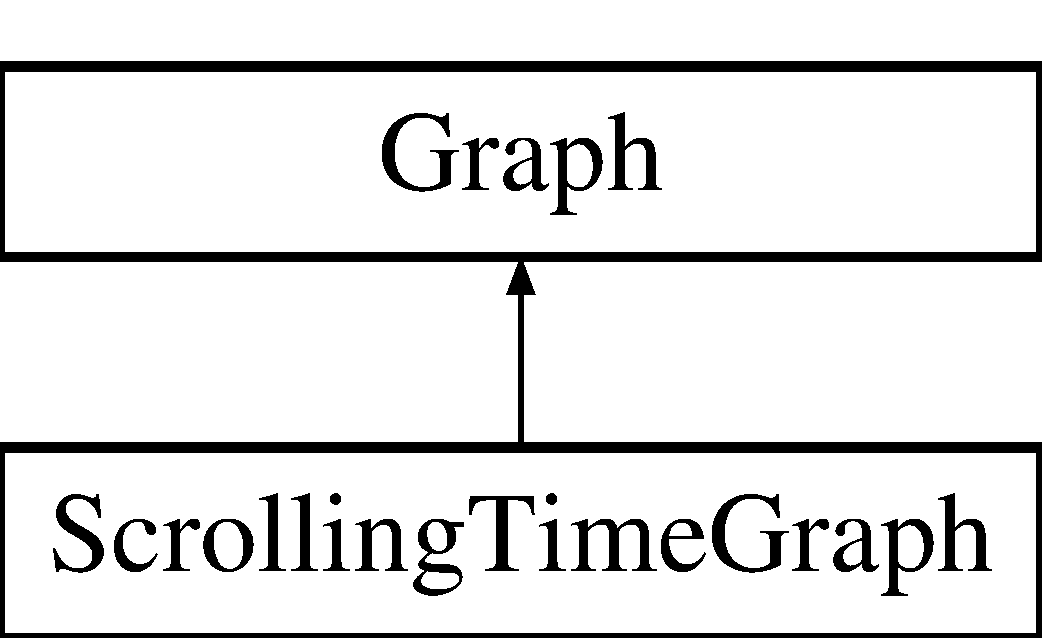
\includegraphics[height=2.000000cm]{class_scrolling_time_graph}
\end{center}
\end{figure}
\subsection*{Public Member Functions}
\begin{DoxyCompactItemize}
\item 
\hyperlink{class_scrolling_time_graph_ac7af242514d5770d99d90743a24163ca}{Scrolling\+Time\+Graph} (Q\+Main\+Window $\ast$main\+Window, \hyperlink{class_q_custom_plot}{Q\+Custom\+Plot} $\ast$main\+Plot, \hyperlink{class_q_custom_plot}{Q\+Custom\+Plot} $\ast$aux\+Plot, Q\+Color primary\+Color, Q\+Color secondary\+Color, Q\+String display\+Unit, int num\+Display\+Values)
\begin{DoxyCompactList}\small\item\em \hyperlink{class_scrolling_time_graph_ac7af242514d5770d99d90743a24163ca}{Scrolling\+Time\+Graph\+::\+Scrolling\+Time\+Graph} Constructs the \hyperlink{class_scrolling_time_graph}{Scrolling\+Time\+Graph}. \end{DoxyCompactList}\item 
void \hyperlink{class_scrolling_time_graph_af26f732b60d98c521ea93709db8f70cc}{add\+Data} (double time, double primary\+Data, double second\+Dary\+Data, int max\+Value=-\/1)
\begin{DoxyCompactList}\small\item\em \hyperlink{class_scrolling_time_graph_af26f732b60d98c521ea93709db8f70cc}{Scrolling\+Time\+Graph\+::add\+Data} Adds two data points to both plots at the given time. \end{DoxyCompactList}\item 
void \hyperlink{class_scrolling_time_graph_a651e6922d732be7084c207cc94257bd7}{set\+Fill} (Q\+Color fill\+Color)
\begin{DoxyCompactList}\small\item\em \hyperlink{class_scrolling_time_graph_a651e6922d732be7084c207cc94257bd7}{Scrolling\+Time\+Graph\+::set\+Fill} Sets the fill between two lines. \end{DoxyCompactList}\item 
Q\+String \hyperlink{class_scrolling_time_graph_a3d0314f268e3eeb7396733147f710ef0}{max\+Display} () override
\begin{DoxyCompactList}\small\item\em \hyperlink{class_scrolling_time_graph_a3d0314f268e3eeb7396733147f710ef0}{Scrolling\+Time\+Graph\+::max\+Display} Returns a string showing the maximum values seen by this graph so far, with units. \end{DoxyCompactList}\item 
Q\+String \hyperlink{class_scrolling_time_graph_ae27ff79b4314b792ecdd27fc6115e0bf}{current\+Display} () override
\begin{DoxyCompactList}\small\item\em \hyperlink{class_scrolling_time_graph_ae27ff79b4314b792ecdd27fc6115e0bf}{Scrolling\+Time\+Graph\+::current\+Display} Returns a string showing the most recent values seen by this graph. with units. \end{DoxyCompactList}\end{DoxyCompactItemize}
\subsection*{Additional Inherited Members}


\subsection{Detailed Description}
The \hyperlink{class_scrolling_time_graph}{Scrolling\+Time\+Graph} class, which inherits from the \hyperlink{class_graph}{Graph} class. This represents a graph with time as the x axis, that \char`\"{}scrolls\char`\"{} with time, showing a sliding window of values. The y axis represents whatever value this graph displays. 

\subsection{Constructor \& Destructor Documentation}
\hypertarget{class_scrolling_time_graph_ac7af242514d5770d99d90743a24163ca}{}\label{class_scrolling_time_graph_ac7af242514d5770d99d90743a24163ca} 
\index{Scrolling\+Time\+Graph@{Scrolling\+Time\+Graph}!Scrolling\+Time\+Graph@{Scrolling\+Time\+Graph}}
\index{Scrolling\+Time\+Graph@{Scrolling\+Time\+Graph}!Scrolling\+Time\+Graph@{Scrolling\+Time\+Graph}}
\subsubsection{\texorpdfstring{Scrolling\+Time\+Graph()}{ScrollingTimeGraph()}}
{\footnotesize\ttfamily Scrolling\+Time\+Graph\+::\+Scrolling\+Time\+Graph (\begin{DoxyParamCaption}\item[{Q\+Main\+Window $\ast$}]{main\+Window,  }\item[{\hyperlink{class_q_custom_plot}{Q\+Custom\+Plot} $\ast$}]{main\+Plot,  }\item[{\hyperlink{class_q_custom_plot}{Q\+Custom\+Plot} $\ast$}]{aux\+Plot,  }\item[{Q\+Color}]{primary\+Color,  }\item[{Q\+Color}]{secondary\+Color,  }\item[{Q\+String}]{display\+Unit,  }\item[{int}]{num\+Display\+Values }\end{DoxyParamCaption})}



\hyperlink{class_scrolling_time_graph_ac7af242514d5770d99d90743a24163ca}{Scrolling\+Time\+Graph\+::\+Scrolling\+Time\+Graph} Constructs the \hyperlink{class_scrolling_time_graph}{Scrolling\+Time\+Graph}. 


\begin{DoxyParams}{Parameters}
{\em main\+Window} & A pointer to the main\+Window, used for connecting ranges of the graph. \\
\hline
{\em main\+Plot} & The main plot for this graph. \\
\hline
{\em aux\+Plot} & The auxiliary plot for this graph, which lives in the sidebar. \\
\hline
{\em primary\+Color} & The color of the primary line of this graph. \\
\hline
{\em secondary\+Color} & The color of the secondary line of this graph. \\
\hline
{\em display\+Unit} & The units to use in displays. \\
\hline
{\em num\+Display\+Values} & The number of values to display in max\+Display and current\+Display. \\
\hline
\end{DoxyParams}


\subsection{Member Function Documentation}
\hypertarget{class_scrolling_time_graph_af26f732b60d98c521ea93709db8f70cc}{}\label{class_scrolling_time_graph_af26f732b60d98c521ea93709db8f70cc} 
\index{Scrolling\+Time\+Graph@{Scrolling\+Time\+Graph}!add\+Data@{add\+Data}}
\index{add\+Data@{add\+Data}!Scrolling\+Time\+Graph@{Scrolling\+Time\+Graph}}
\subsubsection{\texorpdfstring{add\+Data()}{addData()}}
{\footnotesize\ttfamily void Scrolling\+Time\+Graph\+::add\+Data (\begin{DoxyParamCaption}\item[{double}]{time,  }\item[{double}]{primary\+Data,  }\item[{double}]{secondary\+Data,  }\item[{int}]{max\+Value = {\ttfamily -\/1} }\end{DoxyParamCaption})}



\hyperlink{class_scrolling_time_graph_af26f732b60d98c521ea93709db8f70cc}{Scrolling\+Time\+Graph\+::add\+Data} Adds two data points to both plots at the given time. 


\begin{DoxyParams}{Parameters}
{\em time} & The x-\/axis value for the new points. \\
\hline
{\em primary\+Data} & The y-\/value of the point to add to the primary line. \\
\hline
{\em secondary\+Data} & The y-\/value of the point to add to the secondary line. \\
\hline
{\em max\+Value} & The maximum expected y-\/value on the graph. If this is set to a negative number, this is disregarded, and the plots resize dynamically to accomodate real values. \\
\hline
\end{DoxyParams}
\hypertarget{class_scrolling_time_graph_ae27ff79b4314b792ecdd27fc6115e0bf}{}\label{class_scrolling_time_graph_ae27ff79b4314b792ecdd27fc6115e0bf} 
\index{Scrolling\+Time\+Graph@{Scrolling\+Time\+Graph}!current\+Display@{current\+Display}}
\index{current\+Display@{current\+Display}!Scrolling\+Time\+Graph@{Scrolling\+Time\+Graph}}
\subsubsection{\texorpdfstring{current\+Display()}{currentDisplay()}}
{\footnotesize\ttfamily Q\+String Scrolling\+Time\+Graph\+::current\+Display (\begin{DoxyParamCaption}{ }\end{DoxyParamCaption})\hspace{0.3cm}{\ttfamily [override]}, {\ttfamily [virtual]}}



\hyperlink{class_scrolling_time_graph_ae27ff79b4314b792ecdd27fc6115e0bf}{Scrolling\+Time\+Graph\+::current\+Display} Returns a string showing the most recent values seen by this graph. with units. 

\begin{DoxyReturn}{Returns}
The string which contains the most recent values seen by this graph. 
\end{DoxyReturn}


Reimplemented from \hyperlink{class_graph}{Graph}.

\hypertarget{class_scrolling_time_graph_a3d0314f268e3eeb7396733147f710ef0}{}\label{class_scrolling_time_graph_a3d0314f268e3eeb7396733147f710ef0} 
\index{Scrolling\+Time\+Graph@{Scrolling\+Time\+Graph}!max\+Display@{max\+Display}}
\index{max\+Display@{max\+Display}!Scrolling\+Time\+Graph@{Scrolling\+Time\+Graph}}
\subsubsection{\texorpdfstring{max\+Display()}{maxDisplay()}}
{\footnotesize\ttfamily Q\+String Scrolling\+Time\+Graph\+::max\+Display (\begin{DoxyParamCaption}{ }\end{DoxyParamCaption})\hspace{0.3cm}{\ttfamily [override]}, {\ttfamily [virtual]}}



\hyperlink{class_scrolling_time_graph_a3d0314f268e3eeb7396733147f710ef0}{Scrolling\+Time\+Graph\+::max\+Display} Returns a string showing the maximum values seen by this graph so far, with units. 

\begin{DoxyReturn}{Returns}
The string which contains the maximum values seen by this graph. 
\end{DoxyReturn}


Reimplemented from \hyperlink{class_graph}{Graph}.

\hypertarget{class_scrolling_time_graph_a651e6922d732be7084c207cc94257bd7}{}\label{class_scrolling_time_graph_a651e6922d732be7084c207cc94257bd7} 
\index{Scrolling\+Time\+Graph@{Scrolling\+Time\+Graph}!set\+Fill@{set\+Fill}}
\index{set\+Fill@{set\+Fill}!Scrolling\+Time\+Graph@{Scrolling\+Time\+Graph}}
\subsubsection{\texorpdfstring{set\+Fill()}{setFill()}}
{\footnotesize\ttfamily void Scrolling\+Time\+Graph\+::set\+Fill (\begin{DoxyParamCaption}\item[{Q\+Color}]{fill\+Color }\end{DoxyParamCaption})}



\hyperlink{class_scrolling_time_graph_a651e6922d732be7084c207cc94257bd7}{Scrolling\+Time\+Graph\+::set\+Fill} Sets the fill between two lines. 


\begin{DoxyParams}{Parameters}
{\em fill\+Color} & The color to set the fill to. \\
\hline
\end{DoxyParams}


The documentation for this class was generated from the following files\+:\begin{DoxyCompactItemize}
\item 
F\+E\+S\+S-\/\+G\+U\+I/graph.\+h\item 
F\+E\+S\+S-\/\+G\+U\+I/graph.\+cpp\end{DoxyCompactItemize}

\hypertarget{class_serial_device}{}\section{Serial\+Device Class Reference}
\label{class_serial_device}\index{Serial\+Device@{Serial\+Device}}
Inheritance diagram for Serial\+Device\+:\begin{figure}[H]
\begin{center}
\leavevmode
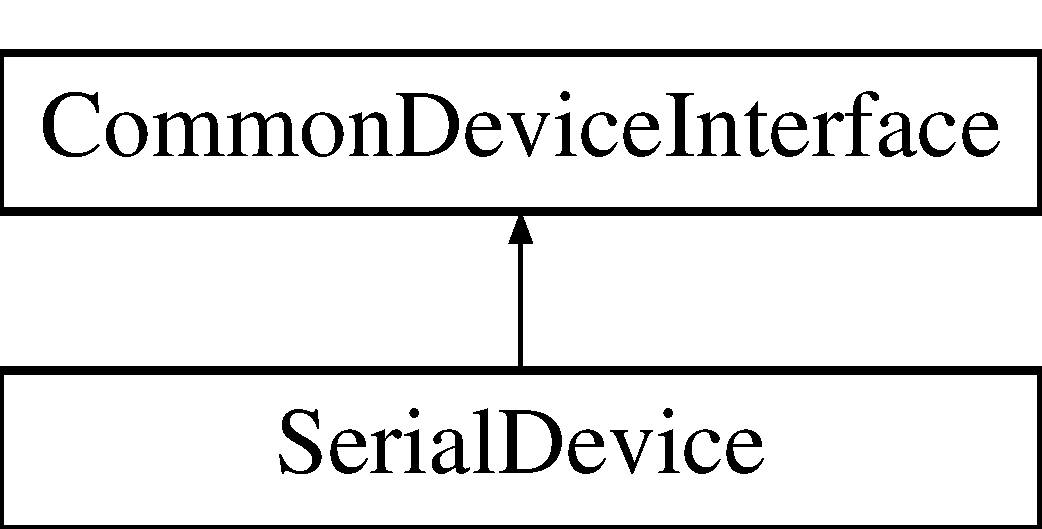
\includegraphics[height=2.000000cm]{class_serial_device}
\end{center}
\end{figure}
\subsection*{Public Member Functions}
\begin{DoxyCompactItemize}
\item 
\hypertarget{class_serial_device_aa0b6d87aea8d882096abe85fda113b26}{}\label{class_serial_device_aa0b6d87aea8d882096abe85fda113b26} 
{\bfseries Serial\+Device} (Q\+Serial\+Port\+Info)
\item 
\hypertarget{class_serial_device_acd6d42b1547bef45569e20ba75cd024a}{}\label{class_serial_device_acd6d42b1547bef45569e20ba75cd024a} 
{\bfseries Serial\+Device} (Q\+Serial\+Port\+Info, int, int, int, int, int)
\item 
\hypertarget{class_serial_device_a070f0759c102570004f1c5e1feb31abe}{}\label{class_serial_device_a070f0759c102570004f1c5e1feb31abe} 
{\bfseries Serial\+Device} (Q\+String)
\item 
\hypertarget{class_serial_device_ade7e1d81fe4768ca9f04b12513d7e316}{}\label{class_serial_device_ade7e1d81fe4768ca9f04b12513d7e316} 
{\bfseries Serial\+Device} (Q\+String, int, int, int, int, int)
\item 
\hypertarget{class_serial_device_aef900fa759c9beb4cfb0c72701eb1876}{}\label{class_serial_device_aef900fa759c9beb4cfb0c72701eb1876} 
void {\bfseries sync} ()
\item 
\hypertarget{class_serial_device_aa2435fb76a612b2ebf1a61287deee85d}{}\label{class_serial_device_aa2435fb76a612b2ebf1a61287deee85d} 
bool {\bfseries is\+Ready} ()
\item 
\hypertarget{class_serial_device_a6940a33b7c8f4b83438d16cfa7d8d3ff}{}\label{class_serial_device_a6940a33b7c8f4b83438d16cfa7d8d3ff} 
bool {\bfseries start\+Device} ()
\item 
\hypertarget{class_serial_device_a55f94898f33ab4674c138fa2cb2e75a1}{}\label{class_serial_device_a55f94898f33ab4674c138fa2cb2e75a1} 
void {\bfseries stop\+Device} ()
\item 
\hypertarget{class_serial_device_a08a8a19f8a25c1dc7593c91afc7d55bd}{}\label{class_serial_device_a08a8a19f8a25c1dc7593c91afc7d55bd} 
void {\bfseries set\+Defaults} ()
\item 
\hypertarget{class_serial_device_ae9fc540188704dbdbf3e75d482a92b86}{}\label{class_serial_device_ae9fc540188704dbdbf3e75d482a92b86} 
bool {\bfseries empty} ()
\item 
\hypertarget{class_serial_device_a0e2d400d48238e451de7725e494a0d47}{}\label{class_serial_device_a0e2d400d48238e451de7725e494a0d47} 
void {\bfseries flush} ()
\item 
\hypertarget{class_serial_device_aa8c488f8088ec59d161744b6600c2467}{}\label{class_serial_device_aa8c488f8088ec59d161744b6600c2467} 
void {\bfseries push\+Int} (int)
\item 
\hypertarget{class_serial_device_a43ed2e28372b856b48f2d2468971009d}{}\label{class_serial_device_a43ed2e28372b856b48f2d2468971009d} 
void {\bfseries push\+Float} (float)
\item 
\hypertarget{class_serial_device_afd99c289e7d6dced96d0e436b317a791}{}\label{class_serial_device_afd99c289e7d6dced96d0e436b317a791} 
void {\bfseries push\+Command} (flybyte)
\item 
\hypertarget{class_serial_device_ae24793cd2c237147faf54f07796fdb7e}{}\label{class_serial_device_ae24793cd2c237147faf54f07796fdb7e} 
void {\bfseries push\+Command\+Immediate} (flybyte)
\item 
\hypertarget{class_serial_device_afb083c91c19b5acdbfd0a8324c646bbf}{}\label{class_serial_device_afb083c91c19b5acdbfd0a8324c646bbf} 
int {\bfseries pop\+Int} ()
\item 
\hypertarget{class_serial_device_a86b2c14bab81f0f9d78d90b57626ef90}{}\label{class_serial_device_a86b2c14bab81f0f9d78d90b57626ef90} 
float {\bfseries pop\+Float} ()
\item 
\hypertarget{class_serial_device_a87ee440731e488ff33bda31947c6a303}{}\label{class_serial_device_a87ee440731e488ff33bda31947c6a303} 
flybyte {\bfseries pop\+Command} ()
\item 
\hypertarget{class_serial_device_a97092ec9379ed561866dad21475ea331}{}\label{class_serial_device_a97092ec9379ed561866dad21475ea331} 
Q\+String {\bfseries name} ()
\item 
\hypertarget{class_serial_device_a38f5d9bc555bb1df0a4c8413e494d4b3}{}\label{class_serial_device_a38f5d9bc555bb1df0a4c8413e494d4b3} 
void {\bfseries set\+Device} (int)
\item 
\hypertarget{class_serial_device_af06c6a34b54819e71186243a38606280}{}\label{class_serial_device_af06c6a34b54819e71186243a38606280} 
void {\bfseries set\+Baud\+Rate} (int)
\item 
\hypertarget{class_serial_device_a91e293977d5401ededf350e19846b5a1}{}\label{class_serial_device_a91e293977d5401ededf350e19846b5a1} 
void {\bfseries set\+Parity} (int)
\item 
\hypertarget{class_serial_device_a74968289347c6ede64587287bb0cf699}{}\label{class_serial_device_a74968289347c6ede64587287bb0cf699} 
void {\bfseries set\+Flow\+Control} (int)
\item 
\hypertarget{class_serial_device_ad0ddca3e77e1d1d4df7c68e83f1ecd91}{}\label{class_serial_device_ad0ddca3e77e1d1d4df7c68e83f1ecd91} 
void {\bfseries set\+Data\+Bits} (int)
\item 
\hypertarget{class_serial_device_a95b44d8167ae0a6a025ba9c4f2d5ee47}{}\label{class_serial_device_a95b44d8167ae0a6a025ba9c4f2d5ee47} 
void {\bfseries set\+Stop\+Bits} (int)
\item 
\hypertarget{class_serial_device_a1440b389cc1bba66e9854a32a5807a8f}{}\label{class_serial_device_a1440b389cc1bba66e9854a32a5807a8f} 
void {\bfseries set\+Port} (Q\+Serial\+Port\+Info)
\end{DoxyCompactItemize}


The documentation for this class was generated from the following files\+:\begin{DoxyCompactItemize}
\item 
F\+E\+S\+S-\/\+G\+U\+I/serialdevice.\+h\item 
F\+E\+S\+S-\/\+G\+U\+I/serialdevice.\+cpp\end{DoxyCompactItemize}

\hypertarget{class_set_password_dialog}{}\section{Set\+Password\+Dialog Class Reference}
\label{class_set_password_dialog}\index{Set\+Password\+Dialog@{Set\+Password\+Dialog}}


The \hyperlink{class_set_password_dialog}{Set\+Password\+Dialog} class Represents a dialog for setting and resetting passwords.  




{\ttfamily \#include $<$setpassworddialog.\+h$>$}

Inheritance diagram for Set\+Password\+Dialog\+:\begin{figure}[H]
\begin{center}
\leavevmode
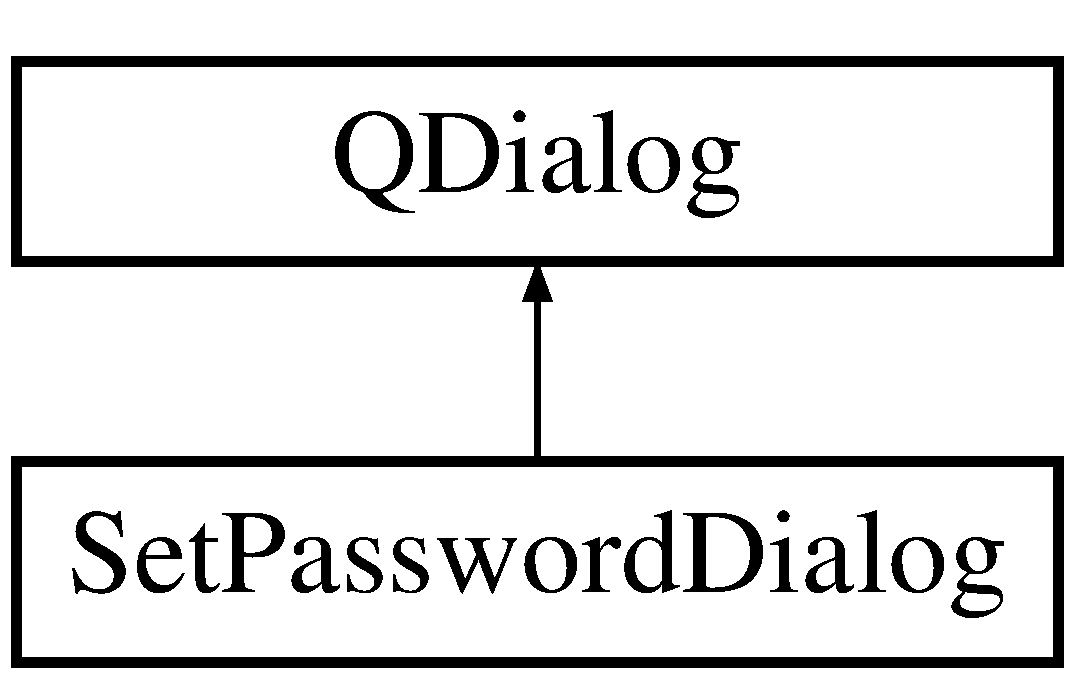
\includegraphics[height=2.000000cm]{class_set_password_dialog}
\end{center}
\end{figure}
\subsection*{Public Member Functions}
\begin{DoxyCompactItemize}
\item 
\hyperlink{class_set_password_dialog_a6c0f4e419cde5431401dd4deeccb1a54}{Set\+Password\+Dialog} (Q\+Widget $\ast$parent=0)
\begin{DoxyCompactList}\small\item\em \hyperlink{class_set_password_dialog_a6c0f4e419cde5431401dd4deeccb1a54}{Set\+Password\+Dialog\+::\+Set\+Password\+Dialog} Constructs the object. \end{DoxyCompactList}\item 
\hyperlink{class_set_password_dialog_ae3dec5f6c8b27800757c928e7e61468c}{$\sim$\+Set\+Password\+Dialog} ()
\begin{DoxyCompactList}\small\item\em \hyperlink{class_set_password_dialog_ae3dec5f6c8b27800757c928e7e61468c}{Set\+Password\+Dialog\+::$\sim$\+Set\+Password\+Dialog} Destructs the object. \end{DoxyCompactList}\end{DoxyCompactItemize}


\subsection{Detailed Description}
The \hyperlink{class_set_password_dialog}{Set\+Password\+Dialog} class Represents a dialog for setting and resetting passwords. 

\subsection{Constructor \& Destructor Documentation}
\hypertarget{class_set_password_dialog_a6c0f4e419cde5431401dd4deeccb1a54}{}\label{class_set_password_dialog_a6c0f4e419cde5431401dd4deeccb1a54} 
\index{Set\+Password\+Dialog@{Set\+Password\+Dialog}!Set\+Password\+Dialog@{Set\+Password\+Dialog}}
\index{Set\+Password\+Dialog@{Set\+Password\+Dialog}!Set\+Password\+Dialog@{Set\+Password\+Dialog}}
\subsubsection{\texorpdfstring{Set\+Password\+Dialog()}{SetPasswordDialog()}}
{\footnotesize\ttfamily Set\+Password\+Dialog\+::\+Set\+Password\+Dialog (\begin{DoxyParamCaption}\item[{Q\+Widget $\ast$}]{parent = {\ttfamily 0} }\end{DoxyParamCaption})\hspace{0.3cm}{\ttfamily [explicit]}}



\hyperlink{class_set_password_dialog_a6c0f4e419cde5431401dd4deeccb1a54}{Set\+Password\+Dialog\+::\+Set\+Password\+Dialog} Constructs the object. 


\begin{DoxyParams}{Parameters}
{\em parent} & The parent widget (should be the main\+Window). \\
\hline
\end{DoxyParams}
\hypertarget{class_set_password_dialog_ae3dec5f6c8b27800757c928e7e61468c}{}\label{class_set_password_dialog_ae3dec5f6c8b27800757c928e7e61468c} 
\index{Set\+Password\+Dialog@{Set\+Password\+Dialog}!````~Set\+Password\+Dialog@{$\sim$\+Set\+Password\+Dialog}}
\index{````~Set\+Password\+Dialog@{$\sim$\+Set\+Password\+Dialog}!Set\+Password\+Dialog@{Set\+Password\+Dialog}}
\subsubsection{\texorpdfstring{$\sim$\+Set\+Password\+Dialog()}{~SetPasswordDialog()}}
{\footnotesize\ttfamily Set\+Password\+Dialog\+::$\sim$\+Set\+Password\+Dialog (\begin{DoxyParamCaption}{ }\end{DoxyParamCaption})}



\hyperlink{class_set_password_dialog_ae3dec5f6c8b27800757c928e7e61468c}{Set\+Password\+Dialog\+::$\sim$\+Set\+Password\+Dialog} Destructs the object. 



The documentation for this class was generated from the following files\+:\begin{DoxyCompactItemize}
\item 
F\+E\+S\+S-\/\+G\+U\+I/\hyperlink{setpassworddialog_8h}{setpassworddialog.\+h}\item 
F\+E\+S\+S-\/\+G\+U\+I/\hyperlink{setpassworddialog_8cpp}{setpassworddialog.\+cpp}\end{DoxyCompactItemize}

\hypertarget{struct_q_c_p_axis_painter_private_1_1_tick_label_data}{}\section{Q\+C\+P\+Axis\+Painter\+Private\+:\+:Tick\+Label\+Data Struct Reference}
\label{struct_q_c_p_axis_painter_private_1_1_tick_label_data}\index{Q\+C\+P\+Axis\+Painter\+Private\+::\+Tick\+Label\+Data@{Q\+C\+P\+Axis\+Painter\+Private\+::\+Tick\+Label\+Data}}
\subsection*{Public Attributes}
\begin{DoxyCompactItemize}
\item 
\hypertarget{struct_q_c_p_axis_painter_private_1_1_tick_label_data_ad65b76a5cafc412179a20b5d79809fc4}{}\label{struct_q_c_p_axis_painter_private_1_1_tick_label_data_ad65b76a5cafc412179a20b5d79809fc4} 
Q\+String {\bfseries base\+Part}
\item 
\hypertarget{struct_q_c_p_axis_painter_private_1_1_tick_label_data_a09692e4ea092137278b4ac051d5fdf2b}{}\label{struct_q_c_p_axis_painter_private_1_1_tick_label_data_a09692e4ea092137278b4ac051d5fdf2b} 
Q\+String {\bfseries exp\+Part}
\item 
\hypertarget{struct_q_c_p_axis_painter_private_1_1_tick_label_data_aac1047ae6ab8e9f5a42923082aabfff5}{}\label{struct_q_c_p_axis_painter_private_1_1_tick_label_data_aac1047ae6ab8e9f5a42923082aabfff5} 
Q\+Rect {\bfseries base\+Bounds}
\item 
\hypertarget{struct_q_c_p_axis_painter_private_1_1_tick_label_data_a6722d2bcefb93011e9dc42301b966846}{}\label{struct_q_c_p_axis_painter_private_1_1_tick_label_data_a6722d2bcefb93011e9dc42301b966846} 
Q\+Rect {\bfseries exp\+Bounds}
\item 
\hypertarget{struct_q_c_p_axis_painter_private_1_1_tick_label_data_afbb3163cf4c628914f1b703945419ea5}{}\label{struct_q_c_p_axis_painter_private_1_1_tick_label_data_afbb3163cf4c628914f1b703945419ea5} 
Q\+Rect {\bfseries total\+Bounds}
\item 
\hypertarget{struct_q_c_p_axis_painter_private_1_1_tick_label_data_aa4d38c5ea47c9184a78ee33ae7f1012e}{}\label{struct_q_c_p_axis_painter_private_1_1_tick_label_data_aa4d38c5ea47c9184a78ee33ae7f1012e} 
Q\+Rect {\bfseries rotated\+Total\+Bounds}
\item 
\hypertarget{struct_q_c_p_axis_painter_private_1_1_tick_label_data_a0d4958a706debaa8d19a9b65fc090d56}{}\label{struct_q_c_p_axis_painter_private_1_1_tick_label_data_a0d4958a706debaa8d19a9b65fc090d56} 
Q\+Font {\bfseries base\+Font}
\item 
\hypertarget{struct_q_c_p_axis_painter_private_1_1_tick_label_data_adc10767ebcb719d6927c012a38b9d933}{}\label{struct_q_c_p_axis_painter_private_1_1_tick_label_data_adc10767ebcb719d6927c012a38b9d933} 
Q\+Font {\bfseries exp\+Font}
\end{DoxyCompactItemize}


The documentation for this struct was generated from the following file\+:\begin{DoxyCompactItemize}
\item 
F\+E\+S\+S-\/\+G\+U\+I/\hyperlink{qcustomplot_8h}{qcustomplot.\+h}\end{DoxyCompactItemize}

\hypertarget{class_transmit_buffer}{}\section{Transmit\+Buffer Class Reference}
\label{class_transmit_buffer}\index{Transmit\+Buffer@{Transmit\+Buffer}}


The Transmit Buffer Class Provides queueing for the communication packets and raw output of packets for interfaces.  




{\ttfamily \#include $<$transmitbuffer.\+h$>$}

\subsection*{Public Member Functions}
\begin{DoxyCompactItemize}
\item 
\hyperlink{class_transmit_buffer_adb5f67b087b5c8d1996f9f7b6fb42341}{Transmit\+Buffer} ()
\begin{DoxyCompactList}\small\item\em \hyperlink{class_transmit_buffer_adb5f67b087b5c8d1996f9f7b6fb42341}{Transmit\+Buffer\+::\+Transmit\+Buffer} Provided if needed in the future, currently no functionality. \end{DoxyCompactList}\item 
\hyperlink{class_transmit_buffer_a9de4adf2b6fef27e9f35ce3392fb12d2}{$\sim$\+Transmit\+Buffer} ()
\begin{DoxyCompactList}\small\item\em \hyperlink{class_transmit_buffer_a9de4adf2b6fef27e9f35ce3392fb12d2}{Transmit\+Buffer\+::$\sim$\+Transmit\+Buffer} Provided if needed in the future, currently no functionality. \end{DoxyCompactList}\item 
void \hyperlink{class_transmit_buffer_aa7966064a6abaeb5ff3f7c8ff0402ec3}{push\+Byte} (\hyperlink{conversions_8h_a1f006e31a957accfe6aa1bf6f401efce}{Fly\+Byte})
\begin{DoxyCompactList}\small\item\em \hyperlink{class_transmit_buffer_aa7966064a6abaeb5ff3f7c8ff0402ec3}{Transmit\+Buffer\+::push\+Byte} Takes bytes until there are enough to build a packet. It converts the bytes to a packet and adds the packet to the packet queue. \end{DoxyCompactList}\item 
void \hyperlink{class_transmit_buffer_a002757b58f4227167db20c8977bbdb28}{push\+Packet} (\hyperlink{class_fly_packet}{Fly\+Packet})
\begin{DoxyCompactList}\small\item\em \hyperlink{class_transmit_buffer_a002757b58f4227167db20c8977bbdb28}{Transmit\+Buffer\+::push\+Packet} Adds the packets to the packet queue. \end{DoxyCompactList}\item 
\hyperlink{conversions_8h_a1f006e31a957accfe6aa1bf6f401efce}{Fly\+Byte} \hyperlink{class_transmit_buffer_a6da9417079dd783d996af8fcc138149c}{pop\+Byte} ()
\begin{DoxyCompactList}\small\item\em \hyperlink{class_transmit_buffer_a6da9417079dd783d996af8fcc138149c}{Transmit\+Buffer\+::pop\+Byte} Get the Byte at the front of the output byte queue created from a packet. \end{DoxyCompactList}\item 
\hyperlink{class_fly_packet}{Fly\+Packet} \hyperlink{class_transmit_buffer_add84c61a7f2f060d236feab584babc64}{pop\+Packet} ()
\begin{DoxyCompactList}\small\item\em \hyperlink{class_transmit_buffer_add84c61a7f2f060d236feab584babc64}{Transmit\+Buffer\+::pop\+Packet} Adds the packets to the packet queue. \end{DoxyCompactList}\item 
void \hyperlink{class_transmit_buffer_a574f5ab5eca07b5ee8a517812cd7d87a}{flush} ()
\begin{DoxyCompactList}\small\item\em \hyperlink{class_transmit_buffer_a574f5ab5eca07b5ee8a517812cd7d87a}{Transmit\+Buffer\+::flush} Empties all internal queues. \end{DoxyCompactList}\item 
bool \hyperlink{class_transmit_buffer_aec08c2e6aa511bfd87d83ec4226b2c8e}{bytes\+Available} ()
\begin{DoxyCompactList}\small\item\em \hyperlink{class_transmit_buffer_aec08c2e6aa511bfd87d83ec4226b2c8e}{Transmit\+Buffer\+::bytes\+Available} Checks if the byte and packet queues are empty. \end{DoxyCompactList}\item 
bool \hyperlink{class_transmit_buffer_aad9976b2ae40b1405a319de979b09827}{packets\+Available} ()
\begin{DoxyCompactList}\small\item\em \hyperlink{class_transmit_buffer_aad9976b2ae40b1405a319de979b09827}{Transmit\+Buffer\+::packets\+Available} Checks if the packet queue is empty. \end{DoxyCompactList}\end{DoxyCompactItemize}


\subsection{Detailed Description}
The Transmit Buffer Class Provides queueing for the communication packets and raw output of packets for interfaces. 

\subsection{Constructor \& Destructor Documentation}
\hypertarget{class_transmit_buffer_adb5f67b087b5c8d1996f9f7b6fb42341}{}\label{class_transmit_buffer_adb5f67b087b5c8d1996f9f7b6fb42341} 
\index{Transmit\+Buffer@{Transmit\+Buffer}!Transmit\+Buffer@{Transmit\+Buffer}}
\index{Transmit\+Buffer@{Transmit\+Buffer}!Transmit\+Buffer@{Transmit\+Buffer}}
\subsubsection{\texorpdfstring{Transmit\+Buffer()}{TransmitBuffer()}}
{\footnotesize\ttfamily Transmit\+Buffer\+::\+Transmit\+Buffer (\begin{DoxyParamCaption}{ }\end{DoxyParamCaption})}



\hyperlink{class_transmit_buffer_adb5f67b087b5c8d1996f9f7b6fb42341}{Transmit\+Buffer\+::\+Transmit\+Buffer} Provided if needed in the future, currently no functionality. 

\hypertarget{class_transmit_buffer_a9de4adf2b6fef27e9f35ce3392fb12d2}{}\label{class_transmit_buffer_a9de4adf2b6fef27e9f35ce3392fb12d2} 
\index{Transmit\+Buffer@{Transmit\+Buffer}!````~Transmit\+Buffer@{$\sim$\+Transmit\+Buffer}}
\index{````~Transmit\+Buffer@{$\sim$\+Transmit\+Buffer}!Transmit\+Buffer@{Transmit\+Buffer}}
\subsubsection{\texorpdfstring{$\sim$\+Transmit\+Buffer()}{~TransmitBuffer()}}
{\footnotesize\ttfamily Transmit\+Buffer\+::$\sim$\+Transmit\+Buffer (\begin{DoxyParamCaption}{ }\end{DoxyParamCaption})}



\hyperlink{class_transmit_buffer_a9de4adf2b6fef27e9f35ce3392fb12d2}{Transmit\+Buffer\+::$\sim$\+Transmit\+Buffer} Provided if needed in the future, currently no functionality. 



\subsection{Member Function Documentation}
\hypertarget{class_transmit_buffer_aec08c2e6aa511bfd87d83ec4226b2c8e}{}\label{class_transmit_buffer_aec08c2e6aa511bfd87d83ec4226b2c8e} 
\index{Transmit\+Buffer@{Transmit\+Buffer}!bytes\+Available@{bytes\+Available}}
\index{bytes\+Available@{bytes\+Available}!Transmit\+Buffer@{Transmit\+Buffer}}
\subsubsection{\texorpdfstring{bytes\+Available()}{bytesAvailable()}}
{\footnotesize\ttfamily bool Transmit\+Buffer\+::bytes\+Available (\begin{DoxyParamCaption}{ }\end{DoxyParamCaption})}



\hyperlink{class_transmit_buffer_aec08c2e6aa511bfd87d83ec4226b2c8e}{Transmit\+Buffer\+::bytes\+Available} Checks if the byte and packet queues are empty. 

\begin{DoxyReturn}{Returns}
bool (true=yes $\vert$ false=no) 
\end{DoxyReturn}
\hypertarget{class_transmit_buffer_a574f5ab5eca07b5ee8a517812cd7d87a}{}\label{class_transmit_buffer_a574f5ab5eca07b5ee8a517812cd7d87a} 
\index{Transmit\+Buffer@{Transmit\+Buffer}!flush@{flush}}
\index{flush@{flush}!Transmit\+Buffer@{Transmit\+Buffer}}
\subsubsection{\texorpdfstring{flush()}{flush()}}
{\footnotesize\ttfamily void Transmit\+Buffer\+::flush (\begin{DoxyParamCaption}{ }\end{DoxyParamCaption})}



\hyperlink{class_transmit_buffer_a574f5ab5eca07b5ee8a517812cd7d87a}{Transmit\+Buffer\+::flush} Empties all internal queues. 

\hypertarget{class_transmit_buffer_aad9976b2ae40b1405a319de979b09827}{}\label{class_transmit_buffer_aad9976b2ae40b1405a319de979b09827} 
\index{Transmit\+Buffer@{Transmit\+Buffer}!packets\+Available@{packets\+Available}}
\index{packets\+Available@{packets\+Available}!Transmit\+Buffer@{Transmit\+Buffer}}
\subsubsection{\texorpdfstring{packets\+Available()}{packetsAvailable()}}
{\footnotesize\ttfamily bool Transmit\+Buffer\+::packets\+Available (\begin{DoxyParamCaption}{ }\end{DoxyParamCaption})}



\hyperlink{class_transmit_buffer_aad9976b2ae40b1405a319de979b09827}{Transmit\+Buffer\+::packets\+Available} Checks if the packet queue is empty. 

\begin{DoxyReturn}{Returns}
bool (true=yes $\vert$ false=no) 
\end{DoxyReturn}
\hypertarget{class_transmit_buffer_a6da9417079dd783d996af8fcc138149c}{}\label{class_transmit_buffer_a6da9417079dd783d996af8fcc138149c} 
\index{Transmit\+Buffer@{Transmit\+Buffer}!pop\+Byte@{pop\+Byte}}
\index{pop\+Byte@{pop\+Byte}!Transmit\+Buffer@{Transmit\+Buffer}}
\subsubsection{\texorpdfstring{pop\+Byte()}{popByte()}}
{\footnotesize\ttfamily \hyperlink{conversions_8h_a1f006e31a957accfe6aa1bf6f401efce}{Fly\+Byte} Transmit\+Buffer\+::pop\+Byte (\begin{DoxyParamCaption}{ }\end{DoxyParamCaption})}



\hyperlink{class_transmit_buffer_a6da9417079dd783d996af8fcc138149c}{Transmit\+Buffer\+::pop\+Byte} Get the Byte at the front of the output byte queue created from a packet. 

\begin{DoxyReturn}{Returns}
Fly\+Byte (First byte in the output queue) 
\end{DoxyReturn}
\hypertarget{class_transmit_buffer_add84c61a7f2f060d236feab584babc64}{}\label{class_transmit_buffer_add84c61a7f2f060d236feab584babc64} 
\index{Transmit\+Buffer@{Transmit\+Buffer}!pop\+Packet@{pop\+Packet}}
\index{pop\+Packet@{pop\+Packet}!Transmit\+Buffer@{Transmit\+Buffer}}
\subsubsection{\texorpdfstring{pop\+Packet()}{popPacket()}}
{\footnotesize\ttfamily \hyperlink{class_fly_packet}{Fly\+Packet} Transmit\+Buffer\+::pop\+Packet (\begin{DoxyParamCaption}{ }\end{DoxyParamCaption})}



\hyperlink{class_transmit_buffer_add84c61a7f2f060d236feab584babc64}{Transmit\+Buffer\+::pop\+Packet} Adds the packets to the packet queue. 

\begin{DoxyReturn}{Returns}
\hyperlink{class_fly_packet}{Fly\+Packet} (Gets a packet from the front of the packet queue) 
\end{DoxyReturn}
\hypertarget{class_transmit_buffer_aa7966064a6abaeb5ff3f7c8ff0402ec3}{}\label{class_transmit_buffer_aa7966064a6abaeb5ff3f7c8ff0402ec3} 
\index{Transmit\+Buffer@{Transmit\+Buffer}!push\+Byte@{push\+Byte}}
\index{push\+Byte@{push\+Byte}!Transmit\+Buffer@{Transmit\+Buffer}}
\subsubsection{\texorpdfstring{push\+Byte()}{pushByte()}}
{\footnotesize\ttfamily void Transmit\+Buffer\+::push\+Byte (\begin{DoxyParamCaption}\item[{\hyperlink{conversions_8h_a1f006e31a957accfe6aa1bf6f401efce}{Fly\+Byte}}]{incoming\+Byte }\end{DoxyParamCaption})}



\hyperlink{class_transmit_buffer_aa7966064a6abaeb5ff3f7c8ff0402ec3}{Transmit\+Buffer\+::push\+Byte} Takes bytes until there are enough to build a packet. It converts the bytes to a packet and adds the packet to the packet queue. 


\begin{DoxyParams}{Parameters}
{\em Fly\+Byte} & (Added to the incoming queue) \\
\hline
\end{DoxyParams}
\hypertarget{class_transmit_buffer_a002757b58f4227167db20c8977bbdb28}{}\label{class_transmit_buffer_a002757b58f4227167db20c8977bbdb28} 
\index{Transmit\+Buffer@{Transmit\+Buffer}!push\+Packet@{push\+Packet}}
\index{push\+Packet@{push\+Packet}!Transmit\+Buffer@{Transmit\+Buffer}}
\subsubsection{\texorpdfstring{push\+Packet()}{pushPacket()}}
{\footnotesize\ttfamily void Transmit\+Buffer\+::push\+Packet (\begin{DoxyParamCaption}\item[{\hyperlink{class_fly_packet}{Fly\+Packet}}]{incoming\+Packet }\end{DoxyParamCaption})}



\hyperlink{class_transmit_buffer_a002757b58f4227167db20c8977bbdb28}{Transmit\+Buffer\+::push\+Packet} Adds the packets to the packet queue. 


\begin{DoxyParams}{Parameters}
{\em \hyperlink{class_fly_packet}{Fly\+Packet}} & (Added to the Packet Queue) \\
\hline
\end{DoxyParams}


The documentation for this class was generated from the following files\+:\begin{DoxyCompactItemize}
\item 
F\+E\+S\+S-\/\+G\+U\+I/\hyperlink{transmitbuffer_8h}{transmitbuffer.\+h}\item 
F\+E\+S\+S-\/\+G\+U\+I/\hyperlink{transmitbuffer_8cpp}{transmitbuffer.\+cpp}\end{DoxyCompactItemize}

\chapter{File Documentation}
\hypertarget{qcustomplot_8cpp}{}\section{C\+:/\+Users/\+Jesse Jutson/\+Documents/\+Git\+Hub/\+F\+E\+S\+S\+G\+U\+I/\+F\+E\+S\+S-\/\+G\+U\+I/qcustomplot.cpp File Reference}
\label{qcustomplot_8cpp}\index{C\+:/\+Users/\+Jesse Jutson/\+Documents/\+Git\+Hub/\+F\+E\+S\+S\+G\+U\+I/\+F\+E\+S\+S-\/\+G\+U\+I/qcustomplot.\+cpp@{C\+:/\+Users/\+Jesse Jutson/\+Documents/\+Git\+Hub/\+F\+E\+S\+S\+G\+U\+I/\+F\+E\+S\+S-\/\+G\+U\+I/qcustomplot.\+cpp}}
{\ttfamily \#include \char`\"{}qcustomplot.\+h\char`\"{}}\newline

\hypertarget{qcustomplot_8h}{}\section{F\+E\+S\+S-\/\+G\+U\+I/qcustomplot.h File Reference}
\label{qcustomplot_8h}\index{F\+E\+S\+S-\/\+G\+U\+I/qcustomplot.\+h@{F\+E\+S\+S-\/\+G\+U\+I/qcustomplot.\+h}}
{\ttfamily \#include $<$Q\+Object$>$}\newline
{\ttfamily \#include $<$Q\+Pointer$>$}\newline
{\ttfamily \#include $<$Q\+Widget$>$}\newline
{\ttfamily \#include $<$Q\+Painter$>$}\newline
{\ttfamily \#include $<$Q\+Paint\+Event$>$}\newline
{\ttfamily \#include $<$Q\+Mouse\+Event$>$}\newline
{\ttfamily \#include $<$Q\+Pixmap$>$}\newline
{\ttfamily \#include $<$Q\+Vector$>$}\newline
{\ttfamily \#include $<$Q\+String$>$}\newline
{\ttfamily \#include $<$Q\+Date\+Time$>$}\newline
{\ttfamily \#include $<$Q\+Multi\+Map$>$}\newline
{\ttfamily \#include $<$Q\+Flags$>$}\newline
{\ttfamily \#include $<$Q\+Debug$>$}\newline
{\ttfamily \#include $<$Q\+Vector2D$>$}\newline
{\ttfamily \#include $<$Q\+Stack$>$}\newline
{\ttfamily \#include $<$Q\+Cache$>$}\newline
{\ttfamily \#include $<$Q\+Margins$>$}\newline
{\ttfamily \#include $<$qmath.\+h$>$}\newline
{\ttfamily \#include $<$limits$>$}\newline
{\ttfamily \#include $<$Qt\+Numeric$>$}\newline
{\ttfamily \#include $<$Qt\+Print\+Support/\+Qt\+Print\+Support$>$}\newline
\subsection*{Classes}
\begin{DoxyCompactItemize}
\item 
class \hyperlink{class_q_c_p_scatter_style}{Q\+C\+P\+Scatter\+Style}
\begin{DoxyCompactList}\small\item\em Represents the visual appearance of scatter points. \end{DoxyCompactList}\item 
class \hyperlink{class_q_c_p_painter}{Q\+C\+P\+Painter}
\begin{DoxyCompactList}\small\item\em Q\+Painter subclass used internally. \end{DoxyCompactList}\item 
class \hyperlink{class_q_c_p_layer}{Q\+C\+P\+Layer}
\begin{DoxyCompactList}\small\item\em A layer that may contain objects, to control the rendering order. \end{DoxyCompactList}\item 
class \hyperlink{class_q_c_p_layerable}{Q\+C\+P\+Layerable}
\begin{DoxyCompactList}\small\item\em Base class for all drawable objects. \end{DoxyCompactList}\item 
class \hyperlink{class_q_c_p_range}{Q\+C\+P\+Range}
\begin{DoxyCompactList}\small\item\em Represents the range an axis is encompassing. \end{DoxyCompactList}\item 
class \hyperlink{class_q_c_p_margin_group}{Q\+C\+P\+Margin\+Group}
\begin{DoxyCompactList}\small\item\em A margin group allows synchronization of margin sides if working with multiple layout elements. \end{DoxyCompactList}\item 
class \hyperlink{class_q_c_p_layout_element}{Q\+C\+P\+Layout\+Element}
\begin{DoxyCompactList}\small\item\em The abstract base class for all objects that form the layout system. \end{DoxyCompactList}\item 
class \hyperlink{class_q_c_p_layout}{Q\+C\+P\+Layout}
\begin{DoxyCompactList}\small\item\em The abstract base class for layouts. \end{DoxyCompactList}\item 
class \hyperlink{class_q_c_p_layout_grid}{Q\+C\+P\+Layout\+Grid}
\begin{DoxyCompactList}\small\item\em A layout that arranges child elements in a grid. \end{DoxyCompactList}\item 
class \hyperlink{class_q_c_p_layout_inset}{Q\+C\+P\+Layout\+Inset}
\begin{DoxyCompactList}\small\item\em A layout that places child elements aligned to the border or arbitrarily positioned. \end{DoxyCompactList}\item 
class \hyperlink{class_q_c_p_line_ending}{Q\+C\+P\+Line\+Ending}
\begin{DoxyCompactList}\small\item\em Handles the different ending decorations for line-\/like items. \end{DoxyCompactList}\item 
class \hyperlink{class_q_c_p_grid}{Q\+C\+P\+Grid}
\begin{DoxyCompactList}\small\item\em Responsible for drawing the grid of a \hyperlink{class_q_c_p_axis}{Q\+C\+P\+Axis}. \end{DoxyCompactList}\item 
class \hyperlink{class_q_c_p_axis}{Q\+C\+P\+Axis}
\begin{DoxyCompactList}\small\item\em Manages a single axis inside a \hyperlink{class_q_custom_plot}{Q\+Custom\+Plot}. \end{DoxyCompactList}\item 
class \hyperlink{class_q_c_p_axis_painter_private}{Q\+C\+P\+Axis\+Painter\+Private}
\item 
struct \hyperlink{struct_q_c_p_axis_painter_private_1_1_cached_label}{Q\+C\+P\+Axis\+Painter\+Private\+::\+Cached\+Label}
\item 
struct \hyperlink{struct_q_c_p_axis_painter_private_1_1_tick_label_data}{Q\+C\+P\+Axis\+Painter\+Private\+::\+Tick\+Label\+Data}
\item 
class \hyperlink{class_q_c_p_abstract_plottable}{Q\+C\+P\+Abstract\+Plottable}
\begin{DoxyCompactList}\small\item\em The abstract base class for all data representing objects in a plot. \end{DoxyCompactList}\item 
class \hyperlink{class_q_c_p_item_anchor}{Q\+C\+P\+Item\+Anchor}
\begin{DoxyCompactList}\small\item\em An anchor of an item to which positions can be attached to. \end{DoxyCompactList}\item 
class \hyperlink{class_q_c_p_item_position}{Q\+C\+P\+Item\+Position}
\begin{DoxyCompactList}\small\item\em Manages the position of an item. \end{DoxyCompactList}\item 
class \hyperlink{class_q_c_p_abstract_item}{Q\+C\+P\+Abstract\+Item}
\begin{DoxyCompactList}\small\item\em The abstract base class for all items in a plot. \end{DoxyCompactList}\item 
class \hyperlink{class_q_custom_plot}{Q\+Custom\+Plot}
\begin{DoxyCompactList}\small\item\em The central class of the library. This is the Q\+Widget which displays the plot and interacts with the user. \end{DoxyCompactList}\item 
class \hyperlink{class_q_c_p_color_gradient}{Q\+C\+P\+Color\+Gradient}
\begin{DoxyCompactList}\small\item\em Defines a color gradient for use with e.\+g. \hyperlink{class_q_c_p_color_map}{Q\+C\+P\+Color\+Map}. \end{DoxyCompactList}\item 
class \hyperlink{class_q_c_p_axis_rect}{Q\+C\+P\+Axis\+Rect}
\begin{DoxyCompactList}\small\item\em Holds multiple axes and arranges them in a rectangular shape. \end{DoxyCompactList}\item 
class \hyperlink{class_q_c_p_abstract_legend_item}{Q\+C\+P\+Abstract\+Legend\+Item}
\begin{DoxyCompactList}\small\item\em The abstract base class for all entries in a \hyperlink{class_q_c_p_legend}{Q\+C\+P\+Legend}. \end{DoxyCompactList}\item 
class \hyperlink{class_q_c_p_plottable_legend_item}{Q\+C\+P\+Plottable\+Legend\+Item}
\begin{DoxyCompactList}\small\item\em A legend item representing a plottable with an icon and the plottable name. \end{DoxyCompactList}\item 
class \hyperlink{class_q_c_p_legend}{Q\+C\+P\+Legend}
\begin{DoxyCompactList}\small\item\em Manages a legend inside a \hyperlink{class_q_custom_plot}{Q\+Custom\+Plot}. \end{DoxyCompactList}\item 
class \hyperlink{class_q_c_p_plot_title}{Q\+C\+P\+Plot\+Title}
\begin{DoxyCompactList}\small\item\em A layout element displaying a plot title text. \end{DoxyCompactList}\item 
class \hyperlink{class_q_c_p_color_scale_axis_rect_private}{Q\+C\+P\+Color\+Scale\+Axis\+Rect\+Private}
\item 
class \hyperlink{class_q_c_p_color_scale}{Q\+C\+P\+Color\+Scale}
\begin{DoxyCompactList}\small\item\em A color scale for use with color coding data such as \hyperlink{class_q_c_p_color_map}{Q\+C\+P\+Color\+Map}. \end{DoxyCompactList}\item 
class \hyperlink{class_q_c_p_data}{Q\+C\+P\+Data}
\begin{DoxyCompactList}\small\item\em Holds the data of one single data point for \hyperlink{class_q_c_p_graph}{Q\+C\+P\+Graph}. \end{DoxyCompactList}\item 
class \hyperlink{class_q_c_p_graph}{Q\+C\+P\+Graph}
\begin{DoxyCompactList}\small\item\em A plottable representing a graph in a plot. \end{DoxyCompactList}\item 
class \hyperlink{class_q_c_p_curve_data}{Q\+C\+P\+Curve\+Data}
\begin{DoxyCompactList}\small\item\em Holds the data of one single data point for \hyperlink{class_q_c_p_curve}{Q\+C\+P\+Curve}. \end{DoxyCompactList}\item 
class \hyperlink{class_q_c_p_curve}{Q\+C\+P\+Curve}
\begin{DoxyCompactList}\small\item\em A plottable representing a parametric curve in a plot. \end{DoxyCompactList}\item 
class \hyperlink{class_q_c_p_bars_group}{Q\+C\+P\+Bars\+Group}
\begin{DoxyCompactList}\small\item\em Groups multiple \hyperlink{class_q_c_p_bars}{Q\+C\+P\+Bars} together so they appear side by side. \end{DoxyCompactList}\item 
class \hyperlink{class_q_c_p_bar_data}{Q\+C\+P\+Bar\+Data}
\begin{DoxyCompactList}\small\item\em Holds the data of one single data point (one bar) for \hyperlink{class_q_c_p_bars}{Q\+C\+P\+Bars}. \end{DoxyCompactList}\item 
class \hyperlink{class_q_c_p_bars}{Q\+C\+P\+Bars}
\begin{DoxyCompactList}\small\item\em A plottable representing a bar chart in a plot. \end{DoxyCompactList}\item 
class \hyperlink{class_q_c_p_statistical_box}{Q\+C\+P\+Statistical\+Box}
\begin{DoxyCompactList}\small\item\em A plottable representing a single statistical box in a plot. \end{DoxyCompactList}\item 
class \hyperlink{class_q_c_p_color_map_data}{Q\+C\+P\+Color\+Map\+Data}
\begin{DoxyCompactList}\small\item\em Holds the two-\/dimensional data of a \hyperlink{class_q_c_p_color_map}{Q\+C\+P\+Color\+Map} plottable. \end{DoxyCompactList}\item 
class \hyperlink{class_q_c_p_color_map}{Q\+C\+P\+Color\+Map}
\begin{DoxyCompactList}\small\item\em A plottable representing a two-\/dimensional color map in a plot. \end{DoxyCompactList}\item 
class \hyperlink{class_q_c_p_financial_data}{Q\+C\+P\+Financial\+Data}
\begin{DoxyCompactList}\small\item\em Holds the data of one single data point for \hyperlink{class_q_c_p_financial}{Q\+C\+P\+Financial}. \end{DoxyCompactList}\item 
class \hyperlink{class_q_c_p_financial}{Q\+C\+P\+Financial}
\begin{DoxyCompactList}\small\item\em A plottable representing a financial stock chart. \end{DoxyCompactList}\item 
class \hyperlink{class_q_c_p_item_straight_line}{Q\+C\+P\+Item\+Straight\+Line}
\begin{DoxyCompactList}\small\item\em A straight line that spans infinitely in both directions. \end{DoxyCompactList}\item 
class \hyperlink{class_q_c_p_item_line}{Q\+C\+P\+Item\+Line}
\begin{DoxyCompactList}\small\item\em A line from one point to another. \end{DoxyCompactList}\item 
class \hyperlink{class_q_c_p_item_curve}{Q\+C\+P\+Item\+Curve}
\begin{DoxyCompactList}\small\item\em A curved line from one point to another. \end{DoxyCompactList}\item 
class \hyperlink{class_q_c_p_item_rect}{Q\+C\+P\+Item\+Rect}
\begin{DoxyCompactList}\small\item\em A rectangle. \end{DoxyCompactList}\item 
class \hyperlink{class_q_c_p_item_text}{Q\+C\+P\+Item\+Text}
\begin{DoxyCompactList}\small\item\em A text label. \end{DoxyCompactList}\item 
class \hyperlink{class_q_c_p_item_ellipse}{Q\+C\+P\+Item\+Ellipse}
\begin{DoxyCompactList}\small\item\em An ellipse. \end{DoxyCompactList}\item 
class \hyperlink{class_q_c_p_item_pixmap}{Q\+C\+P\+Item\+Pixmap}
\begin{DoxyCompactList}\small\item\em An arbitrary pixmap. \end{DoxyCompactList}\item 
class \hyperlink{class_q_c_p_item_tracer}{Q\+C\+P\+Item\+Tracer}
\begin{DoxyCompactList}\small\item\em Item that sticks to \hyperlink{class_q_c_p_graph}{Q\+C\+P\+Graph} data points. \end{DoxyCompactList}\item 
class \hyperlink{class_q_c_p_item_bracket}{Q\+C\+P\+Item\+Bracket}
\begin{DoxyCompactList}\small\item\em A bracket for referencing/highlighting certain parts in the plot. \end{DoxyCompactList}\end{DoxyCompactItemize}
\subsection*{Namespaces}
\begin{DoxyCompactItemize}
\item 
 \hyperlink{namespace_q_c_p}{Q\+CP}
\end{DoxyCompactItemize}
\subsection*{Typedefs}
\begin{DoxyCompactItemize}
\item 
typedef Q\+Map$<$ double, \hyperlink{class_q_c_p_data}{Q\+C\+P\+Data} $>$ \hyperlink{qcustomplot_8h_a84a9c4a4c2216ccfdcb5f3067cda76e3}{Q\+C\+P\+Data\+Map}
\item 
\hypertarget{qcustomplot_8h_a0fd9a83e0a1783a82f439b0e200b6ae5}{}\label{qcustomplot_8h_a0fd9a83e0a1783a82f439b0e200b6ae5} 
typedef Q\+Map\+Iterator$<$ double, \hyperlink{class_q_c_p_data}{Q\+C\+P\+Data} $>$ {\bfseries Q\+C\+P\+Data\+Map\+Iterator}
\item 
\hypertarget{qcustomplot_8h_a4798b07422d0d4c46a8665c23958b0ea}{}\label{qcustomplot_8h_a4798b07422d0d4c46a8665c23958b0ea} 
typedef Q\+Mutable\+Map\+Iterator$<$ double, \hyperlink{class_q_c_p_data}{Q\+C\+P\+Data} $>$ {\bfseries Q\+C\+P\+Data\+Mutable\+Map\+Iterator}
\item 
typedef Q\+Map$<$ double, \hyperlink{class_q_c_p_curve_data}{Q\+C\+P\+Curve\+Data} $>$ \hyperlink{qcustomplot_8h_a444d37ec9cb2951b3a7fe443c34d1658}{Q\+C\+P\+Curve\+Data\+Map}
\item 
\hypertarget{qcustomplot_8h_aeb3dbc9f09e8ce9957be86dd6e8c803d}{}\label{qcustomplot_8h_aeb3dbc9f09e8ce9957be86dd6e8c803d} 
typedef Q\+Map\+Iterator$<$ double, \hyperlink{class_q_c_p_curve_data}{Q\+C\+P\+Curve\+Data} $>$ {\bfseries Q\+C\+P\+Curve\+Data\+Map\+Iterator}
\item 
\hypertarget{qcustomplot_8h_ad85cf567575500cc8877fd65f4c5b9fb}{}\label{qcustomplot_8h_ad85cf567575500cc8877fd65f4c5b9fb} 
typedef Q\+Mutable\+Map\+Iterator$<$ double, \hyperlink{class_q_c_p_curve_data}{Q\+C\+P\+Curve\+Data} $>$ {\bfseries Q\+C\+P\+Curve\+Data\+Mutable\+Map\+Iterator}
\item 
typedef Q\+Map$<$ double, \hyperlink{class_q_c_p_bar_data}{Q\+C\+P\+Bar\+Data} $>$ \hyperlink{qcustomplot_8h_aa846c77472cae93def9f1609d0c57191}{Q\+C\+P\+Bar\+Data\+Map}
\item 
\hypertarget{qcustomplot_8h_ad8f7e19ade25016f69f2ebedbd130f92}{}\label{qcustomplot_8h_ad8f7e19ade25016f69f2ebedbd130f92} 
typedef Q\+Map\+Iterator$<$ double, \hyperlink{class_q_c_p_bar_data}{Q\+C\+P\+Bar\+Data} $>$ {\bfseries Q\+C\+P\+Bar\+Data\+Map\+Iterator}
\item 
\hypertarget{qcustomplot_8h_a5f61a38b8bb85ebfefa76ae0983f1c78}{}\label{qcustomplot_8h_a5f61a38b8bb85ebfefa76ae0983f1c78} 
typedef Q\+Mutable\+Map\+Iterator$<$ double, \hyperlink{class_q_c_p_bar_data}{Q\+C\+P\+Bar\+Data} $>$ {\bfseries Q\+C\+P\+Bar\+Data\+Mutable\+Map\+Iterator}
\item 
typedef Q\+Map$<$ double, \hyperlink{class_q_c_p_financial_data}{Q\+C\+P\+Financial\+Data} $>$ \hyperlink{qcustomplot_8h_a745c09823fae0974b50beca9bc3b3d7d}{Q\+C\+P\+Financial\+Data\+Map}
\item 
\hypertarget{qcustomplot_8h_ad72fc549e490f52e8cbb03d7891f30c1}{}\label{qcustomplot_8h_ad72fc549e490f52e8cbb03d7891f30c1} 
typedef Q\+Map\+Iterator$<$ double, \hyperlink{class_q_c_p_financial_data}{Q\+C\+P\+Financial\+Data} $>$ {\bfseries Q\+C\+P\+Financial\+Data\+Map\+Iterator}
\item 
\hypertarget{qcustomplot_8h_abfbd4d77d8bc14aa8ada56abcafe6711}{}\label{qcustomplot_8h_abfbd4d77d8bc14aa8ada56abcafe6711} 
typedef Q\+Mutable\+Map\+Iterator$<$ double, \hyperlink{class_q_c_p_financial_data}{Q\+C\+P\+Financial\+Data} $>$ {\bfseries Q\+C\+P\+Financial\+Data\+Mutable\+Map\+Iterator}
\end{DoxyCompactItemize}
\subsection*{Enumerations}
\begin{DoxyCompactItemize}
\item 
enum \hyperlink{namespace_q_c_p_a7e487e3e2ccb62ab7771065bab7cae54}{Q\+C\+P\+::\+Margin\+Side} \{ \newline
\hyperlink{namespace_q_c_p_a7e487e3e2ccb62ab7771065bab7cae54a9500c8bfcc9e80b9dff0a8e00e867f07}{Q\+C\+P\+::ms\+Left} = 0x01, 
\hyperlink{namespace_q_c_p_a7e487e3e2ccb62ab7771065bab7cae54a93c719593bb2b94ed244d52c86d83b65}{Q\+C\+P\+::ms\+Right} = 0x02, 
\hyperlink{namespace_q_c_p_a7e487e3e2ccb62ab7771065bab7cae54a5db8fb0d0b0ecf0d611c2602a348e8a0}{Q\+C\+P\+::ms\+Top} = 0x04, 
\hyperlink{namespace_q_c_p_a7e487e3e2ccb62ab7771065bab7cae54a5241d8eac2bab9524a38889f576179cc}{Q\+C\+P\+::ms\+Bottom} = 0x08, 
\newline
\hyperlink{namespace_q_c_p_a7e487e3e2ccb62ab7771065bab7cae54a43d7361cb0c5244eabdc962021bffebc}{Q\+C\+P\+::ms\+All} = 0x\+FF, 
\hyperlink{namespace_q_c_p_a7e487e3e2ccb62ab7771065bab7cae54a80aa4149f16dabd538f8b2e3d42c42d5}{Q\+C\+P\+::ms\+None} = 0x00
 \}
\item 
enum \hyperlink{namespace_q_c_p_ae55dbe315d41fe80f29ba88100843a0c}{Q\+C\+P\+::\+Antialiased\+Element} \{ \newline
\hyperlink{namespace_q_c_p_ae55dbe315d41fe80f29ba88100843a0caefa92e89cd37f8a081fd2075aa1af73f}{Q\+C\+P\+::ae\+Axes} = 0x0001, 
\hyperlink{namespace_q_c_p_ae55dbe315d41fe80f29ba88100843a0ca4fbb37118d62288af0ca601ff2b07a2f}{Q\+C\+P\+::ae\+Grid} = 0x0002, 
\hyperlink{namespace_q_c_p_ae55dbe315d41fe80f29ba88100843a0caaedf83369188a15a69f92bb1d85ca97b}{Q\+C\+P\+::ae\+Sub\+Grid} = 0x0004, 
\hyperlink{namespace_q_c_p_ae55dbe315d41fe80f29ba88100843a0ca9e0127a6361b5d0596b031a482c5cf97}{Q\+C\+P\+::ae\+Legend} = 0x0008, 
\newline
\hyperlink{namespace_q_c_p_ae55dbe315d41fe80f29ba88100843a0ca1aca7a50c1b95403958733a4acafe773}{Q\+C\+P\+::ae\+Legend\+Items} = 0x0010, 
\hyperlink{namespace_q_c_p_ae55dbe315d41fe80f29ba88100843a0ca4145e4251b0cf2dbedabeea0a38f84f6}{Q\+C\+P\+::ae\+Plottables} = 0x0020, 
\hyperlink{namespace_q_c_p_ae55dbe315d41fe80f29ba88100843a0caf7712a85d6b0c75b24301d2fe9484db3}{Q\+C\+P\+::ae\+Items} = 0x0040, 
\hyperlink{namespace_q_c_p_ae55dbe315d41fe80f29ba88100843a0cae45ed8cd167bffe27d7f40da4bc17e9c}{Q\+C\+P\+::ae\+Scatters} = 0x0080, 
\newline
\hyperlink{namespace_q_c_p_ae55dbe315d41fe80f29ba88100843a0ca9dcf3882cb321bb305f71fdc0f09f63d}{Q\+C\+P\+::ae\+Error\+Bars} = 0x0100, 
\hyperlink{namespace_q_c_p_ae55dbe315d41fe80f29ba88100843a0ca788810f0aa930137de6ad6cc6d83d354}{Q\+C\+P\+::ae\+Fills} = 0x0200, 
\hyperlink{namespace_q_c_p_ae55dbe315d41fe80f29ba88100843a0ca261f8ea78cf3c9561726223ffa33dc12}{Q\+C\+P\+::ae\+Zero\+Line} = 0x0400, 
\hyperlink{namespace_q_c_p_ae55dbe315d41fe80f29ba88100843a0caa897c232a0ffc8368e7c100ffc59ef31}{Q\+C\+P\+::ae\+All} = 0x\+F\+F\+FF, 
\newline
\hyperlink{namespace_q_c_p_ae55dbe315d41fe80f29ba88100843a0caa9e90d81896358757d94275aeaa58f6a}{Q\+C\+P\+::ae\+None} = 0x0000
 \}
\item 
enum \hyperlink{namespace_q_c_p_a5400e5fcb9528d92002ddb938c1f4ef4}{Q\+C\+P\+::\+Plotting\+Hint} \{ \hyperlink{namespace_q_c_p_a5400e5fcb9528d92002ddb938c1f4ef4ab7283c5bfc1ba9e597015389880bda42}{Q\+C\+P\+::ph\+None} = 0x000, 
\hyperlink{namespace_q_c_p_a5400e5fcb9528d92002ddb938c1f4ef4aa5fd227bc878c56ad2a87ea32c74ee4d}{Q\+C\+P\+::ph\+Fast\+Polylines} = 0x001, 
\hyperlink{namespace_q_c_p_a5400e5fcb9528d92002ddb938c1f4ef4aa3090dafa0e0f9a28c579c79d6c2d283}{Q\+C\+P\+::ph\+Force\+Repaint} = 0x002, 
\hyperlink{namespace_q_c_p_a5400e5fcb9528d92002ddb938c1f4ef4a8e9cfe5ee0c5cd36dd7accf9739aff65}{Q\+C\+P\+::ph\+Cache\+Labels} = 0x004
 \}
\item 
enum \hyperlink{namespace_q_c_p_a2ad6bb6281c7c2d593d4277b44c2b037}{Q\+C\+P\+::\+Interaction} \{ \newline
\hyperlink{namespace_q_c_p_a2ad6bb6281c7c2d593d4277b44c2b037a2c4432b9aceafb94000be8d1b589ef18}{Q\+C\+P\+::i\+Range\+Drag} = 0x001, 
\hyperlink{namespace_q_c_p_a2ad6bb6281c7c2d593d4277b44c2b037abee1e94353525a636aeaf0ba32b72e14}{Q\+C\+P\+::i\+Range\+Zoom} = 0x002, 
\hyperlink{namespace_q_c_p_a2ad6bb6281c7c2d593d4277b44c2b037aef673112c5067c3cf4cfddb62da7265d}{Q\+C\+P\+::i\+Multi\+Select} = 0x004, 
\hyperlink{namespace_q_c_p_a2ad6bb6281c7c2d593d4277b44c2b037a67148c8227b4155eca49135fc274c7ec}{Q\+C\+P\+::i\+Select\+Plottables} = 0x008, 
\newline
\hyperlink{namespace_q_c_p_a2ad6bb6281c7c2d593d4277b44c2b037ad6644ac55bef621645326e9dd7469caa}{Q\+C\+P\+::i\+Select\+Axes} = 0x010, 
\hyperlink{namespace_q_c_p_a2ad6bb6281c7c2d593d4277b44c2b037a269c9af298e257d1108edec0432b5513}{Q\+C\+P\+::i\+Select\+Legend} = 0x020, 
\hyperlink{namespace_q_c_p_a2ad6bb6281c7c2d593d4277b44c2b037aea2f7c105d674e76d9b187b02ef29260}{Q\+C\+P\+::i\+Select\+Items} = 0x040, 
\hyperlink{namespace_q_c_p_a2ad6bb6281c7c2d593d4277b44c2b037af67a50bc26147a13b551b3a625374949}{Q\+C\+P\+::i\+Select\+Other} = 0x080
 \}
\end{DoxyCompactItemize}
\subsection*{Functions}
\begin{DoxyCompactItemize}
\item 
\hypertarget{namespace_q_c_p_a07ab701c05329089f933b9cae2638a63}{}\label{namespace_q_c_p_a07ab701c05329089f933b9cae2638a63} 
bool {\bfseries Q\+C\+P\+::is\+Invalid\+Data} (double value)
\item 
\hypertarget{namespace_q_c_p_a728903e5c3dd17847bee280f4005496f}{}\label{namespace_q_c_p_a728903e5c3dd17847bee280f4005496f} 
bool {\bfseries Q\+C\+P\+::is\+Invalid\+Data} (double value1, double value2)
\item 
\hypertarget{namespace_q_c_p_afbf6e3084c108f2bb4372107945ee82f}{}\label{namespace_q_c_p_afbf6e3084c108f2bb4372107945ee82f} 
void {\bfseries Q\+C\+P\+::set\+Margin\+Value} (Q\+Margins \&margins, \hyperlink{namespace_q_c_p_a7e487e3e2ccb62ab7771065bab7cae54}{Q\+C\+P\+::\+Margin\+Side} side, int value)
\item 
\hypertarget{namespace_q_c_p_a23a2679d3495c444acc26acc61e35b5b}{}\label{namespace_q_c_p_a23a2679d3495c444acc26acc61e35b5b} 
int {\bfseries Q\+C\+P\+::get\+Margin\+Value} (const Q\+Margins \&margins, \hyperlink{namespace_q_c_p_a7e487e3e2ccb62ab7771065bab7cae54}{Q\+C\+P\+::\+Margin\+Side} side)
\item 
\hypertarget{qcustomplot_8h_adb726938bdfce1d1136855b9b3613d2e}{}\label{qcustomplot_8h_adb726938bdfce1d1136855b9b3613d2e} 
{\bfseries Q\+\_\+\+D\+E\+C\+L\+A\+R\+E\+\_\+\+T\+Y\+P\+E\+I\+N\+FO} (\hyperlink{class_q_c_p_scatter_style}{Q\+C\+P\+Scatter\+Style}, Q\+\_\+\+M\+O\+V\+A\+B\+L\+E\+\_\+\+T\+Y\+PE)
\item 
\hypertarget{qcustomplot_8h_aed23afce99cb2c82db7540026f3b7af3}{}\label{qcustomplot_8h_aed23afce99cb2c82db7540026f3b7af3} 
{\bfseries Q\+\_\+\+D\+E\+C\+L\+A\+R\+E\+\_\+\+T\+Y\+P\+E\+I\+N\+FO} (\hyperlink{class_q_c_p_range}{Q\+C\+P\+Range}, Q\+\_\+\+M\+O\+V\+A\+B\+L\+E\+\_\+\+T\+Y\+PE)
\item 
const \hyperlink{class_q_c_p_range}{Q\+C\+P\+Range} \hyperlink{qcustomplot_8h_aede14e69c31568a75bd3e9286603c9e0}{operator+} (const \hyperlink{class_q_c_p_range}{Q\+C\+P\+Range} \&range, double value)
\item 
const \hyperlink{class_q_c_p_range}{Q\+C\+P\+Range} \hyperlink{qcustomplot_8h_aa7dd8efde53d115b7107826194879069}{operator+} (double value, const \hyperlink{class_q_c_p_range}{Q\+C\+P\+Range} \&range)
\item 
const \hyperlink{class_q_c_p_range}{Q\+C\+P\+Range} \hyperlink{qcustomplot_8h_a797f82830b516646da8873f82e39e356}{operator-\/} (const \hyperlink{class_q_c_p_range}{Q\+C\+P\+Range} \&range, double value)
\item 
const \hyperlink{class_q_c_p_range}{Q\+C\+P\+Range} \hyperlink{qcustomplot_8h_a558b1248ff6a9e41fd5b2630555a8acc}{operator$\ast$} (const \hyperlink{class_q_c_p_range}{Q\+C\+P\+Range} \&range, double value)
\item 
const \hyperlink{class_q_c_p_range}{Q\+C\+P\+Range} \hyperlink{qcustomplot_8h_a5cb2332f6957021f47cc768089f4f090}{operator$\ast$} (double value, const \hyperlink{class_q_c_p_range}{Q\+C\+P\+Range} \&range)
\item 
const \hyperlink{class_q_c_p_range}{Q\+C\+P\+Range} \hyperlink{qcustomplot_8h_a4b366a3a21974c88e09b0d39d4a24a4b}{operator/} (const \hyperlink{class_q_c_p_range}{Q\+C\+P\+Range} \&range, double value)
\item 
\hypertarget{qcustomplot_8h_a1376c7245cffa4c7a6b945a542473907}{}\label{qcustomplot_8h_a1376c7245cffa4c7a6b945a542473907} 
{\bfseries Q\+\_\+\+D\+E\+C\+L\+A\+R\+E\+\_\+\+T\+Y\+P\+E\+I\+N\+FO} (\hyperlink{class_q_c_p_line_ending}{Q\+C\+P\+Line\+Ending}, Q\+\_\+\+M\+O\+V\+A\+B\+L\+E\+\_\+\+T\+Y\+PE)
\item 
\hypertarget{qcustomplot_8h_ae6c02a20d51ce03bc5dfd27c25a1cc6a}{}\label{qcustomplot_8h_ae6c02a20d51ce03bc5dfd27c25a1cc6a} 
{\bfseries Q\+\_\+\+D\+E\+C\+L\+A\+R\+E\+\_\+\+T\+Y\+P\+E\+I\+N\+FO} (\hyperlink{class_q_c_p_data}{Q\+C\+P\+Data}, Q\+\_\+\+M\+O\+V\+A\+B\+L\+E\+\_\+\+T\+Y\+PE)
\item 
\hypertarget{qcustomplot_8h_a274cda11a63dec5b5796c0cf25efd5d7}{}\label{qcustomplot_8h_a274cda11a63dec5b5796c0cf25efd5d7} 
{\bfseries Q\+\_\+\+D\+E\+C\+L\+A\+R\+E\+\_\+\+T\+Y\+P\+E\+I\+N\+FO} (\hyperlink{class_q_c_p_curve_data}{Q\+C\+P\+Curve\+Data}, Q\+\_\+\+M\+O\+V\+A\+B\+L\+E\+\_\+\+T\+Y\+PE)
\item 
\hypertarget{qcustomplot_8h_a620613bd0461892b290f74997828edae}{}\label{qcustomplot_8h_a620613bd0461892b290f74997828edae} 
{\bfseries Q\+\_\+\+D\+E\+C\+L\+A\+R\+E\+\_\+\+T\+Y\+P\+E\+I\+N\+FO} (\hyperlink{class_q_c_p_bar_data}{Q\+C\+P\+Bar\+Data}, Q\+\_\+\+M\+O\+V\+A\+B\+L\+E\+\_\+\+T\+Y\+PE)
\item 
\hypertarget{qcustomplot_8h_a36893db8c9fcdf5f9fcd8545f686d3ad}{}\label{qcustomplot_8h_a36893db8c9fcdf5f9fcd8545f686d3ad} 
{\bfseries Q\+\_\+\+D\+E\+C\+L\+A\+R\+E\+\_\+\+T\+Y\+P\+E\+I\+N\+FO} (\hyperlink{class_q_c_p_financial_data}{Q\+C\+P\+Financial\+Data}, Q\+\_\+\+M\+O\+V\+A\+B\+L\+E\+\_\+\+T\+Y\+PE)
\end{DoxyCompactItemize}


\subsection{Typedef Documentation}
\hypertarget{qcustomplot_8h_aa846c77472cae93def9f1609d0c57191}{}\label{qcustomplot_8h_aa846c77472cae93def9f1609d0c57191} 
\index{qcustomplot.\+h@{qcustomplot.\+h}!Q\+C\+P\+Bar\+Data\+Map@{Q\+C\+P\+Bar\+Data\+Map}}
\index{Q\+C\+P\+Bar\+Data\+Map@{Q\+C\+P\+Bar\+Data\+Map}!qcustomplot.\+h@{qcustomplot.\+h}}
\subsubsection{\texorpdfstring{Q\+C\+P\+Bar\+Data\+Map}{QCPBarDataMap}}
{\footnotesize\ttfamily \hyperlink{qcustomplot_8h_aa846c77472cae93def9f1609d0c57191}{Q\+C\+P\+Bar\+Data\+Map}}

Container for storing \hyperlink{class_q_c_p_bar_data}{Q\+C\+P\+Bar\+Data} items in a sorted fashion. The key of the map is the key member of the \hyperlink{class_q_c_p_bar_data}{Q\+C\+P\+Bar\+Data} instance.

This is the container in which \hyperlink{class_q_c_p_bars}{Q\+C\+P\+Bars} holds its data. \begin{DoxySeeAlso}{See also}
\hyperlink{class_q_c_p_bar_data}{Q\+C\+P\+Bar\+Data}, \hyperlink{class_q_c_p_bars_aa3435aab19e0a49e4e7b41bd36a8d96b}{Q\+C\+P\+Bars\+::set\+Data} 
\end{DoxySeeAlso}
\hypertarget{qcustomplot_8h_a444d37ec9cb2951b3a7fe443c34d1658}{}\label{qcustomplot_8h_a444d37ec9cb2951b3a7fe443c34d1658} 
\index{qcustomplot.\+h@{qcustomplot.\+h}!Q\+C\+P\+Curve\+Data\+Map@{Q\+C\+P\+Curve\+Data\+Map}}
\index{Q\+C\+P\+Curve\+Data\+Map@{Q\+C\+P\+Curve\+Data\+Map}!qcustomplot.\+h@{qcustomplot.\+h}}
\subsubsection{\texorpdfstring{Q\+C\+P\+Curve\+Data\+Map}{QCPCurveDataMap}}
{\footnotesize\ttfamily \hyperlink{qcustomplot_8h_a444d37ec9cb2951b3a7fe443c34d1658}{Q\+C\+P\+Curve\+Data\+Map}}

Container for storing \hyperlink{class_q_c_p_curve_data}{Q\+C\+P\+Curve\+Data} items in a sorted fashion. The key of the map is the t member of the \hyperlink{class_q_c_p_curve_data}{Q\+C\+P\+Curve\+Data} instance.

This is the container in which \hyperlink{class_q_c_p_curve}{Q\+C\+P\+Curve} holds its data. \begin{DoxySeeAlso}{See also}
\hyperlink{class_q_c_p_curve_data}{Q\+C\+P\+Curve\+Data}, \hyperlink{class_q_c_p_curve_a631ac886708460013b30052f49cbc9da}{Q\+C\+P\+Curve\+::set\+Data} 
\end{DoxySeeAlso}
\hypertarget{qcustomplot_8h_a84a9c4a4c2216ccfdcb5f3067cda76e3}{}\label{qcustomplot_8h_a84a9c4a4c2216ccfdcb5f3067cda76e3} 
\index{qcustomplot.\+h@{qcustomplot.\+h}!Q\+C\+P\+Data\+Map@{Q\+C\+P\+Data\+Map}}
\index{Q\+C\+P\+Data\+Map@{Q\+C\+P\+Data\+Map}!qcustomplot.\+h@{qcustomplot.\+h}}
\subsubsection{\texorpdfstring{Q\+C\+P\+Data\+Map}{QCPDataMap}}
{\footnotesize\ttfamily \hyperlink{qcustomplot_8h_a84a9c4a4c2216ccfdcb5f3067cda76e3}{Q\+C\+P\+Data\+Map}}

Container for storing \hyperlink{class_q_c_p_data}{Q\+C\+P\+Data} items in a sorted fashion. The key of the map is the key member of the \hyperlink{class_q_c_p_data}{Q\+C\+P\+Data} instance.

This is the container in which \hyperlink{class_q_c_p_graph}{Q\+C\+P\+Graph} holds its data. \begin{DoxySeeAlso}{See also}
\hyperlink{class_q_c_p_data}{Q\+C\+P\+Data}, \hyperlink{class_q_c_p_graph_a1df2fd710545c8ba3b2c99a39a27bf8b}{Q\+C\+P\+Graph\+::set\+Data} 
\end{DoxySeeAlso}
\hypertarget{qcustomplot_8h_a745c09823fae0974b50beca9bc3b3d7d}{}\label{qcustomplot_8h_a745c09823fae0974b50beca9bc3b3d7d} 
\index{qcustomplot.\+h@{qcustomplot.\+h}!Q\+C\+P\+Financial\+Data\+Map@{Q\+C\+P\+Financial\+Data\+Map}}
\index{Q\+C\+P\+Financial\+Data\+Map@{Q\+C\+P\+Financial\+Data\+Map}!qcustomplot.\+h@{qcustomplot.\+h}}
\subsubsection{\texorpdfstring{Q\+C\+P\+Financial\+Data\+Map}{QCPFinancialDataMap}}
{\footnotesize\ttfamily \hyperlink{qcustomplot_8h_a745c09823fae0974b50beca9bc3b3d7d}{Q\+C\+P\+Financial\+Data\+Map}}

Container for storing \hyperlink{class_q_c_p_financial_data}{Q\+C\+P\+Financial\+Data} items in a sorted fashion. The key of the map is the key member of the \hyperlink{class_q_c_p_financial_data}{Q\+C\+P\+Financial\+Data} instance.

This is the container in which \hyperlink{class_q_c_p_financial}{Q\+C\+P\+Financial} holds its data. \begin{DoxySeeAlso}{See also}
\hyperlink{class_q_c_p_financial}{Q\+C\+P\+Financial}, \hyperlink{class_q_c_p_financial_adf12a86082f1e488df6a4e8603f8fd6d}{Q\+C\+P\+Financial\+::set\+Data} 
\end{DoxySeeAlso}


\subsection{Function Documentation}
\hypertarget{qcustomplot_8h_a558b1248ff6a9e41fd5b2630555a8acc}{}\label{qcustomplot_8h_a558b1248ff6a9e41fd5b2630555a8acc} 
\index{qcustomplot.\+h@{qcustomplot.\+h}!operator$\ast$@{operator$\ast$}}
\index{operator$\ast$@{operator$\ast$}!qcustomplot.\+h@{qcustomplot.\+h}}
\subsubsection{\texorpdfstring{operator$\ast$()}{operator*()}\hspace{0.1cm}{\footnotesize\ttfamily [1/2]}}
{\footnotesize\ttfamily const \hyperlink{class_q_c_p_range}{Q\+C\+P\+Range} operator$\ast$ (\begin{DoxyParamCaption}\item[{const \hyperlink{class_q_c_p_range}{Q\+C\+P\+Range} \&}]{range,  }\item[{double}]{value }\end{DoxyParamCaption})\hspace{0.3cm}{\ttfamily [inline]}}

Multiplies both boundaries of the range by {\itshape value}. \hypertarget{qcustomplot_8h_a5cb2332f6957021f47cc768089f4f090}{}\label{qcustomplot_8h_a5cb2332f6957021f47cc768089f4f090} 
\index{qcustomplot.\+h@{qcustomplot.\+h}!operator$\ast$@{operator$\ast$}}
\index{operator$\ast$@{operator$\ast$}!qcustomplot.\+h@{qcustomplot.\+h}}
\subsubsection{\texorpdfstring{operator$\ast$()}{operator*()}\hspace{0.1cm}{\footnotesize\ttfamily [2/2]}}
{\footnotesize\ttfamily const \hyperlink{class_q_c_p_range}{Q\+C\+P\+Range} operator$\ast$ (\begin{DoxyParamCaption}\item[{double}]{value,  }\item[{const \hyperlink{class_q_c_p_range}{Q\+C\+P\+Range} \&}]{range }\end{DoxyParamCaption})\hspace{0.3cm}{\ttfamily [inline]}}

Multiplies both boundaries of the range by {\itshape value}. \hypertarget{qcustomplot_8h_aede14e69c31568a75bd3e9286603c9e0}{}\label{qcustomplot_8h_aede14e69c31568a75bd3e9286603c9e0} 
\index{qcustomplot.\+h@{qcustomplot.\+h}!operator+@{operator+}}
\index{operator+@{operator+}!qcustomplot.\+h@{qcustomplot.\+h}}
\subsubsection{\texorpdfstring{operator+()}{operator+()}\hspace{0.1cm}{\footnotesize\ttfamily [1/2]}}
{\footnotesize\ttfamily const \hyperlink{class_q_c_p_range}{Q\+C\+P\+Range} operator+ (\begin{DoxyParamCaption}\item[{const \hyperlink{class_q_c_p_range}{Q\+C\+P\+Range} \&}]{range,  }\item[{double}]{value }\end{DoxyParamCaption})\hspace{0.3cm}{\ttfamily [inline]}}

Adds {\itshape value} to both boundaries of the range. \hypertarget{qcustomplot_8h_aa7dd8efde53d115b7107826194879069}{}\label{qcustomplot_8h_aa7dd8efde53d115b7107826194879069} 
\index{qcustomplot.\+h@{qcustomplot.\+h}!operator+@{operator+}}
\index{operator+@{operator+}!qcustomplot.\+h@{qcustomplot.\+h}}
\subsubsection{\texorpdfstring{operator+()}{operator+()}\hspace{0.1cm}{\footnotesize\ttfamily [2/2]}}
{\footnotesize\ttfamily const \hyperlink{class_q_c_p_range}{Q\+C\+P\+Range} operator+ (\begin{DoxyParamCaption}\item[{double}]{value,  }\item[{const \hyperlink{class_q_c_p_range}{Q\+C\+P\+Range} \&}]{range }\end{DoxyParamCaption})\hspace{0.3cm}{\ttfamily [inline]}}

Adds {\itshape value} to both boundaries of the range. \hypertarget{qcustomplot_8h_a797f82830b516646da8873f82e39e356}{}\label{qcustomplot_8h_a797f82830b516646da8873f82e39e356} 
\index{qcustomplot.\+h@{qcustomplot.\+h}!operator-\/@{operator-\/}}
\index{operator-\/@{operator-\/}!qcustomplot.\+h@{qcustomplot.\+h}}
\subsubsection{\texorpdfstring{operator-\/()}{operator-()}}
{\footnotesize\ttfamily const \hyperlink{class_q_c_p_range}{Q\+C\+P\+Range} operator-\/ (\begin{DoxyParamCaption}\item[{const \hyperlink{class_q_c_p_range}{Q\+C\+P\+Range} \&}]{range,  }\item[{double}]{value }\end{DoxyParamCaption})\hspace{0.3cm}{\ttfamily [inline]}}

Subtracts {\itshape value} from both boundaries of the range. \hypertarget{qcustomplot_8h_a4b366a3a21974c88e09b0d39d4a24a4b}{}\label{qcustomplot_8h_a4b366a3a21974c88e09b0d39d4a24a4b} 
\index{qcustomplot.\+h@{qcustomplot.\+h}!operator/@{operator/}}
\index{operator/@{operator/}!qcustomplot.\+h@{qcustomplot.\+h}}
\subsubsection{\texorpdfstring{operator/()}{operator/()}}
{\footnotesize\ttfamily const \hyperlink{class_q_c_p_range}{Q\+C\+P\+Range} operator/ (\begin{DoxyParamCaption}\item[{const \hyperlink{class_q_c_p_range}{Q\+C\+P\+Range} \&}]{range,  }\item[{double}]{value }\end{DoxyParamCaption})\hspace{0.3cm}{\ttfamily [inline]}}

Divides both boundaries of the range by {\itshape value}. 
%--- End generated contents ---

% Index
\backmatter
\newpage
\phantomsection
\clearemptydoublepage
\addcontentsline{toc}{chapter}{Index}
\printindex

\end{document}
